% main-kdp.tex defines \kdpbuild and inputs this file: the KDP paperback interior, 7 x 10 in trim, no bleed, two sided with chapters opening on the right.
\ifdefined\kdpbuild
\documentclass[11pt,twoside,openright]{book}
\usepackage[paperwidth=7in,paperheight=10in,inner=0.875in,outer=0.75in,top=0.6in,bottom=0.6in,headheight=14pt,headsep=0.25in,footskip=0.35in,includehead,includefoot]{geometry}
\else
\documentclass[11pt,openany,oneside]{book}
\usepackage[margin=1.15in]{geometry}
\fi
\usepackage{amsmath,amssymb,amsthm,mathtools}
\usepackage{graphicx,booktabs,xcolor}
% longtable: the notation tables of Appendix C, the tables of principal results of Chapter 1 and the script tables of Appendix A
% break across pages (a tabular taller than the page runs off its foot); their captions are as wide as those of the floats
\usepackage{longtable}
\setlength{\LTcapwidth}{\textwidth}
\usepackage{needspace}
\usepackage{titlesec}
\usepackage{tocloft}
\usepackage{listings}
\usepackage{tikz}
\usetikzlibrary{positioning}
\usepackage[hidelinks]{hyperref}
\titleclass{\part}{top}
\titleformat{\part}[display]{\normalfont\huge\scshape\centering}{Part \thepart}{0.6em}{}
\titlespacing*{\part}{0pt}{0pt}{2.5em}
\titleformat{\chapter}[display]{\normalfont\LARGE\scshape}{\chaptertitlename\ \thechapter}{0.8em}{}
\titleformat{\section}{\normalfont\large\scshape}{\thesection}{1em}{}
\titleformat{\subsection}{\normalfont\scshape}{\thesubsection}{1em}{}
\titleformat{\paragraph}[runin]{\normalfont\itshape}{}{0pt}{}
\renewcommand{\cftchapfont}{\normalfont}
\renewcommand{\cftchappagefont}{\normalfont}
\renewcommand{\cftpartfont}{\normalfont\scshape}
\renewcommand{\cftpartpagefont}{\normalfont}
\lstset{basicstyle=\ttfamily\footnotesize,breaklines=true,columns=fullflexible,frame=single}
\newtheoremstyle{sc}{6pt}{6pt}{\itshape}{}{\scshape}{.}{0.5em}{}
\newtheoremstyle{scr}{6pt}{6pt}{\normalfont}{}{\scshape}{.}{0.5em}{}
\theoremstyle{sc}
\newtheorem{theorem}{Theorem}[section]
\newtheorem{proposition}[theorem]{Proposition}
\newtheorem{lemma}[theorem]{Lemma}
\newtheorem{corollary}[theorem]{Corollary}
\theoremstyle{scr}
\newtheorem{remark}[theorem]{Remark}
\newtheorem{definition}[theorem]{Definition}
\newtheorem{problem}{Problem}[chapter]
\newtheorem{example}[theorem]{Example}
\newtheorem{question}[theorem]{Question}
\numberwithin{equation}{section}
\hyphenation{deconvolution}
\setcounter{secnumdepth}{3}
\setcounter{tocdepth}{1}
\titleformat{\subsubsection}{\normalfont\itshape}{\thesubsubsection}{1em}{}
% Exercises are collected at the end of each chapter and numbered chapter.n across the groups of the section.
\newcounter{exercise}[chapter]
\newenvironment{exercises}{\setlength{\leftmargini}{3em}\begin{enumerate}\renewcommand{\theenumi}{\thechapter.\arabic{enumi}}\renewcommand{\labelenumi}{\theenumi.}\setcounter{enumi}{\value{exercise}}}{\setcounter{exercise}{\value{enumi}}\end{enumerate}}
\renewcommand{\qedsymbol}{$\square$}
\newcommand{\RH}{\mathrm{RH}}
\newcommand{\re}{\operatorname{Re}}
\newcommand{\im}{\operatorname{Im}}
\newcommand{\tv}[1]{\lVert #1\rVert_{\mathrm{TV}}}
\newcommand{\R}{\mathbb{R}}
\newcommand{\C}{\mathbb{C}}
\newcommand{\E}{\mathbb{E}}
\newcommand{\sech}{\operatorname{sech}}
\newcommand{\sqs}{\sqrt{s}}
\newcommand{\Om}{\Omega}
\newcommand{\HCM}{\mathrm{HCM}}
\newcommand{\GGC}{\mathrm{GGC}}
\newcommand{\cut}{\C\setminus(-\infty,0]}
% \fitwidth{...} sets a table at its natural width and scales it down to the line width only when it is wider (the KDP text block is 0.8 in narrower than that of main.pdf)
\newsavebox{\fitbox}
\newcommand{\fitwidth}[1]{\sbox{\fitbox}{#1}\ifdim\wd\fitbox>\linewidth\resizebox{\linewidth}{!}{\usebox{\fitbox}}\else\usebox{\fitbox}\fi}
\renewcommand{\Re}{\operatorname{Re}}
\renewcommand{\Im}{\operatorname{Im}}
\emergencystretch=3em
\raggedbottom
\renewcommand{\topfraction}{0.9}
\renewcommand{\bottomfraction}{0.8}
\renewcommand{\textfraction}{0.07}
\renewcommand{\floatpagefraction}{0.75}
\setcounter{topnumber}{3}
\setcounter{bottomnumber}{2}
\setcounter{totalnumber}{4}
\makeatletter
\setlength\@fptop{0pt}
\setlength\@fpsep{12pt plus 2fil}
\setlength\@fpbot{0pt plus 1fil}
\makeatother
\ifdefined\kdpbuild
\hypersetup{pdftitle={Computing the Riemann Hypothesis},pdfauthor={Nicholas G. Polson and Vadim Sokolov}}
% running heads: chapter on the left page, section on the right, page numbers outside; a title too long for \small drops to \footnotesize
\usepackage{fancyhdr}
\pagestyle{fancy}
\fancyhf{}
\renewcommand{\headrulewidth}{0pt}
\newsavebox{\kdphead}
\newcommand{\kdpmark}[1]{\sbox{\kdphead}{\small\itshape\nouppercase{#1}}\ifdim\wd\kdphead>\dimexpr\headwidth-3em\relax{\footnotesize\itshape\nouppercase{#1}}\else\usebox{\kdphead}\fi}
\fancyhead[LE,RO]{\small\thepage}
\fancyhead[RE]{\kdpmark{\leftmark}}
\fancyhead[LO]{\kdpmark{\rightmark}}
\fancypagestyle{plain}{\fancyhf{}\fancyfoot[C]{\small\thepage}\renewcommand{\headrulewidth}{0pt}}
\renewcommand{\chaptermark}[1]{\markboth{\thechapter\enspace #1}{\thechapter\enspace #1}}
\renewcommand{\sectionmark}[1]{\markright{\thesection\enspace #1}}
% the blank page before a right hand opening carries no running head
\makeatletter
\renewcommand{\cleardoublepage}{\clearpage\ifodd\c@page\else\hbox{}\thispagestyle{empty}\newpage\fi}
\makeatother
\fi
% the git commit the book is typeset from: version.tex is written before every build by tools/stamp_version.py (see latexmkrc); a missing stamp counts as uncommitted
\InputIfFileExists{version.tex}{}{\def\bookcommit{unknown}\def\bookcommitfull{unknown}\def\bookcommitdate{unknown date}\def\bookbuilddate{\today}\def\bookdirty{1}}
\hypersetup{pdfinfo={Commit={\bookcommitfull}}}
% the release metadata for the copyright page (\BookVersion, \BookYear, \BookDOIline, \BookISBNline): bookmeta.tex is generated from book.yaml by bookrepo.py generate (book-writing skill); it never holds the paperback ISBN, which kdp.py interior defines for the print edition alone
% Generated by bookrepo.py from book.yaml and results.yaml. Edit those files, not this one.
% \BookDOI is empty until zenodo.py reserve; \BookDOIline prints the whole line, or nothing while it is empty (needs hyperref).
% \BookISBN stays empty here: the free KDP ISBN may appear only in the print edition, and kdp.py interior defines it
% for that build alone, so \BookISBNline prints "Paperback ISBN: ..." in print and nothing in the digital edition.
\newcommand*{\BookVersion}{1.2.0}
\newcommand*{\BookEdition}{1}
\newcommand*{\BookYear}{2026}
\newcommand*{\BookDOI}{10.5281/zenodo.23543693}
\newcommand*{\BookDOIline}{Digital Object Identifier (DOI): \href{https://doi.org/10.5281/zenodo.23543693}{\nolinkurl{10.5281/zenodo.23543693}}}
\providecommand*{\BookISBN}{}
\ifx\BookISBN\empty\newcommand*{\BookISBNline}{}\else\newcommand*{\BookISBNline}{Paperback ISBN: \BookISBN}\fi

\ifdefined\kdpbuild\ifnum\bookdirty=1 \AtEndDocument{\PackageWarningNoLine{main}{The KDP interior is not built from a clean commit (commit \bookcommit)}}\fi\fi
\begin{document}
\frontmatter
\ifdefined\kdpbuild
% half title (i), blank (ii), title page (iii), copyright page (iv)
\thispagestyle{empty}
\vspace*{2.2in}
\begin{center}{\LARGE\scshape Computing the Riemann Hypothesis\par}\end{center}
\cleardoublepage
\thispagestyle{empty}
\begin{center}
\vspace*{1.1in}
{\Huge\scshape Computing the\\[0.35em] Riemann Hypothesis\par}
\vspace{0.8cm}
{\Large Thorin Measures, P\'olya Densities\\[0.2em] and Hitting Times\par}
\vspace{2.2cm}
{\large Nicholas G. Polson\par}
{\small Booth School of Business, University of Chicago\par}
\vspace{0.6cm}
{\large Vadim Sokolov\par}
{\small Department of Systems Engineering and Operations Research\\ George Mason University\par}
\end{center}
\clearpage
\thispagestyle{empty}
\vspace*{\fill}
\begin{flushleft}\small
\textit{Computing the Riemann Hypothesis: Thorin Measures, P\'olya Densities and Hitting Times}\\[1em]
Copyright \copyright\ \BookYear\ Nicholas G. Polson and Vadim Sokolov\\[1em]
License: distributed under the Creative Commons Attribution 4.0 International License (CC BY 4.0), \url{https://creativecommons.org/licenses/by/4.0/}: you may copy, share and adapt this book for any purpose, provided you credit the authors. The code is released under the MIT License.\\[1em]
\ifx\BookISBNline\empty\else\BookISBNline\\[1em]\fi
\ifx\BookDOIline\empty\else\BookDOIline\\[1em]\fi
\kdpimprint\\[1em]
First edition, October 2026\\[1em]
Cover: the Thorin density of $\xi(\frac12)/\xi(\frac12+\sqrt u)$ at eight resolutions, computed by the authors.\\[1em]
Source, code and data: \url{https://github.com/VadimSokolov/computing_rh}\\[1em]
Version \BookVersion, typeset by the authors in \LaTeX\ from commit \texttt{\bookcommit} of the source (\bookcommitdate).
\end{flushleft}
\cleardoublepage
\else
\begin{titlepage}
\centering
\vspace*{3cm}
{\Huge\scshape Computing the Riemann Hypothesis\par}
\vspace{0.8cm}
{\Large Thorin Measures, P\'olya Densities and Hitting Times\par}
\vspace{2.5cm}
{\large Nicholas G. Polson\par}
{\small Booth School of Business, University of Chicago\par}
\vspace{0.6cm}
{\large Vadim Sokolov\par}
{\small Department of Systems Engineering and Operations Research, George Mason University\par}
\vfill
{\large Draft of \bookbuilddate\par}
\vspace{0.3cm}
{\normalsize commit \texttt{\bookcommit}\par}
\end{titlepage}
\fi
\chapter*{Preface}
\addcontentsline{toc}{chapter}{Preface}\markboth{\MakeUppercase{Preface}}{\MakeUppercase{Preface}}

The Riemann Hypothesis can be stated as the positivity of a measure. The reciprocal Xi clock $u\mapsto\xi(\frac12)/\xi(\frac12+\sqrt u)$ is the Laplace transform of a generalised gamma convolution exactly when every nontrivial zero lies on the critical line, and then its Thorin measure is the discrete measure $\sum_{\gamma>0}\delta_{\gamma^2}$ on the squared ordinates. This book asks what computation can say about that positivity condition.

Its answer has three parts. First, the Thorin measure is computable at every positive resolution, with explicit error bounds, from the P\'olya kernel alone, with no primes and no list of zeros. Second, the distance between the computed measure and the measure demanded by RH can be measured exactly, and the signature an off line zero would leave can be calibrated. Third, a finite computation could refute RH by certifying a zero off the line, but neither a computation of the zeros up to a finite height nor a finite set of positivity tests on the heat trace can prove it: for every sufficiently large height $R$ such that RH has been verified up to $R+50$, there is a perturbation of $\xi$, with the same order, type and symmetry and the same zeros below $R$, that has zeros off the line between $R$ and $R+50$ and still passes the tests. The book makes this precise and locates the remaining difficulty. A last question is how much of the positivity can be proved. Moved from the centre of the critical strip to the basepoint one, the clock has a positive Thorin measure with no hypothesis. Chapters~\ref{chap:basepoint} to \ref{chap:almost} follow each construction of the book back across the strip as far as it holds unconditionally; below the basepoint one, zero density estimates still show that the zeros to the right of the basepoint, the only possible source of negativity, carry a vanishing fraction of the mass of the density.

The book grew out of the first author's programme on generalised gamma convolutions and the P\'olya density, collected in the monograph \emph{On Hilbert's 8th Problem} \cite{P26}, and out of a joint paper computing the Thorin measure directly \cite{PS26}. The first author's arXiv paper of the same title is a separate work, which we cite by version: \cite{P17} is its version 24, of 2026, and \cite{P17v5} its version 5, of 2017. Chapters~\ref{chap:rzeta} and \ref{chap:rzid} incorporate Part IX of that monograph \cite{P26}, the first author's work on the reciprocal zeta function, written as the manuscript \cite{P26rz}, and Chapters~\ref{chap:basepoint} to \ref{chap:almost} a paper of the authors on the reciprocal Xi function at the basepoint one and across the critical strip, together with notes on Riesz's criterion and on almost generalised gamma convolutions. Sections~\ref{ch:chi12} and \ref{ch:bpeta} draw on a manuscript of the first author on the Thorin measures of the Dedekind eta function \cite{P26eta}, and Chapter~\ref{chap:ferro} on a note of the first author on ferromagnetic random variables. The core evaluator runs in ball arithmetic, and Appendix~\ref{app:code} describes the scripts and data files behind the tables and figures and what the archive lacks. No proof of RH is claimed.

\bigskip
\noindent Chicago and Fairfax, September 2026

\tableofcontents
\listoffigures
\listoftables
\mainmatter
\chapter{Introduction and foundations}\label{chap:foundations}

The book rests on one equivalence, between the Riemann Hypothesis and the positivity of the Thorin measure of a function built from the completed zeta function.

\section{The Thorin condition and what this book shows}\label{ch:intro}

Write $\xi(s)=\frac12s(s-1)\pi^{-s/2}\Gamma(s/2)\zeta(s)$ for the completed zeta function. It is entire of order one, real on the real axis and on the critical line, symmetric under $s\mapsto1-s$, and its zeros are the nontrivial zeros $\rho$ of $\zeta$. The Riemann Hypothesis (RH) asserts that every $\rho$ has real part $\frac12$.

This book works with a reformulation. Put
\[
G(u)=\frac{\xi(\frac12+\sqrt u)}{\xi(\frac12)} .
\]
Because $\xi(\frac12+s)$ is even in $s$, $G$ is an entire function of $u$ with no branch point, of order one half, and Hadamard's theorem gives
\[
G(u)=\prod_k\Big(1+\frac u{a_k}\Big),\qquad a_k=-(\rho_k-\tfrac12)^2,
\]
one factor for each pair $\{\rho,1-\rho\}$ (Section~\ref{ch:clock} derives the product as \eqref{eq:ch2:hadamard}). A zero on the line has $a_k=\gamma_k^2>0$; a zero off the line has $a_k$ complex. The reciprocal $1/G$ is the \emph{clock}. The classical theory of generalised gamma convolutions (GGC) of Thorin and Bondesson \cite{Thorin77a,Thorin,Bondesson} says that a function of the form $\exp\{-\int\log(1+u/z)\,U(dz)\}$ with a positive measure $U$ is the Laplace transform of a positive random variable, and that $U$, the Thorin measure, is unique. The rigidity theorem of \cite{P26}, which Section~\ref{ch:clock} restates with its source as Proposition~\ref{prop:rigid}, says that the clock $u\mapsto\xi(\frac12)/\xi(\frac12+\sqrt u)$ is the Laplace transform of a generalised gamma convolution if and only if RH holds, and that its Thorin measure is then
\begin{equation}\label{eq:URH}
U_{\RH}=\sum_{\gamma>0}\delta_{\gamma^2},
\end{equation}
while the clock variable is $T=\sum_{\gamma>0}e_\gamma/\gamma^2$ with independent standard exponentials $e_\gamma$.

We call the requirement that the Thorin measure of the clock be a positive measure the \emph{Thorin condition}. It has several equivalent faces, each of which is a sign condition. The logarithmic derivative $G'/G(u)=\sum_k(u+a_k)^{-1}$ must be a Stieltjes transform. The heat trace $W(t)=\sum_ke^{-a_kt}$ must be completely monotone. The Thorin density $\rho_\varepsilon(\theta)=\pi^{-1}\re(\xi'/\xi)(\frac12+\varepsilon+i\theta)$ at every resolution $\varepsilon>0$ must be nonnegative, which is Lagarias's criterion \cite{Lagarias}; for $\varepsilon\ge\frac12$, where the basepoint $\frac12+\varepsilon$ is at least one, it is positive with no hypothesis (Section~\ref{ch:basepoint}). Weil's explicit formula functional must be positive on positive definite test functions \cite{Weil52}. The clock must be hyperbolically completely monotone (Corollary~\ref{cor:hcm}). All of these say the same thing, and all of them are, at a finite resolution and on a finite window, computable. Section~\ref{sec:ch3:diag} turns them into tests and compares how well each locates a failure (Table~\ref{tab:ch3:diag}).

\subsection{What computation can and cannot say}

Computation has a long history in the study of RH. Riemann computed the first zeros by hand \cite{Siegel32}. Gram \cite{Gram03}, Backlund \cite{Backlund14}, Hutchinson \cite{Hutchinson25} and Titchmarsh \cite{Titchmarsh36} extended the tables \cite[Chapters 6 to 8]{Edwards}; Turing gave the method that certifies a count without evaluating off the line \cite{Turing53}; Lehmer found the near coincident pairs \cite{Lehmer56} that bound the de Bruijn Newman constant \cite{CSV94}; Odlyzko computed zeros near the $10^{12}$th zero, at height about $2.7\times10^{11}$, and tested their statistics against random matrix theory \cite{Odlyzko87}, and later computed zeros near the $10^{20}$th, at height about $1.5\times10^{19}$ \cite{Odlyzko92}, and beyond \cite{Odlyzko01}; Platt and Trudgian verified RH below height $3\times10^{12}$ \cite{PT21}. Appendix~\ref{app:history} tells this history, with the landmarks in Table~\ref{tab:appB}. None of it proves RH, and the reason is structural rather than technological: every computation sees finitely many zeros, and there are functions with the order, type and symmetry of $\xi$ that pass a given finite set of heat trace tests and yet have zeros off the line just above any sufficiently large height $R$ for which RH has been verified up to $R+50$ (Theorem~\ref{thm:ch13:perturb} \cite[Theorem D]{P17}).

The Thorin condition gives computation a different role. Instead of locating zeros one at a time, it asks for the sign of a measure, and the measure can be computed at every positive resolution without knowing where a single zero is. The questions then become quantitative. How close, in which metric, is the computed Thorin measure to the discrete RH measure? At what resolution does an off line zero become visible, and with what signature? What does the explicit formula say about the cost of computing the Thorin measure from the primes? Which limiting procedures preserve positivity and which do not? And since positivity is a theorem once the basepoint is moved from $\frac12$ to one, how much of it survives as the basepoint moves back across the critical strip? The book answers these questions, the last of them in Chapters~\ref{chap:basepoint} to \ref{chap:almost}.

Three ways of evaluating $\xi$ appear throughout. The first is P\'olya's integral, $\Xi(\theta)=\int\Phi(u)\cos(\theta u)\,du$, with the P\'olya kernel $\Phi$, a positive, doubly exponentially decaying function built from the Jacobi theta function. The integral is exact and needs no primes and no zeros, and since $\Phi$ is analytic in a strip the trapezoid rule applied to it is spectrally accurate; the cost is the cancellation $e^{-\pi\theta/4}$, which the tilted contour of Section~\ref{ch:polya} largely removes. The second is the Riemann Siegel formula and its fast multi point descendant, the Odlyzko Sch\"onhage algorithm \cite{OS88}, the tools of choice at large height. The third is the explicit formula, which evaluates the same objects from the primes and the gamma factor; the sine squared lemma is its Thorin form.

The principle that ties them together is that the Thorin measure at resolution $\varepsilon$ is the Poisson smoothing of the zeros, and simultaneously the sine squared image of the primes. The first description makes it computable from any evaluator of $\xi$ off the line. The second explains why the primes alone cannot compute it near the line. In Selberg's smoothed explicit formula the prime cutoff $x$ plays the part of the resolution: if no zero has real part greater than $\frac12$, the error at resolution $\varepsilon$ is of order $x^{-\varepsilon}/(\varepsilon^2\log x)$, so that $k$ correct digits need $x\approx10^{k/\varepsilon}$, with primes up to $x^2$ (Section~\ref{sec:ch10:selberg}). Figure~\ref{fig:ch1:flow} shows the first description at work: the Thorin measure at decreasing resolution, sharpening onto the zeros.

\begin{figure}[htbp]
\centering
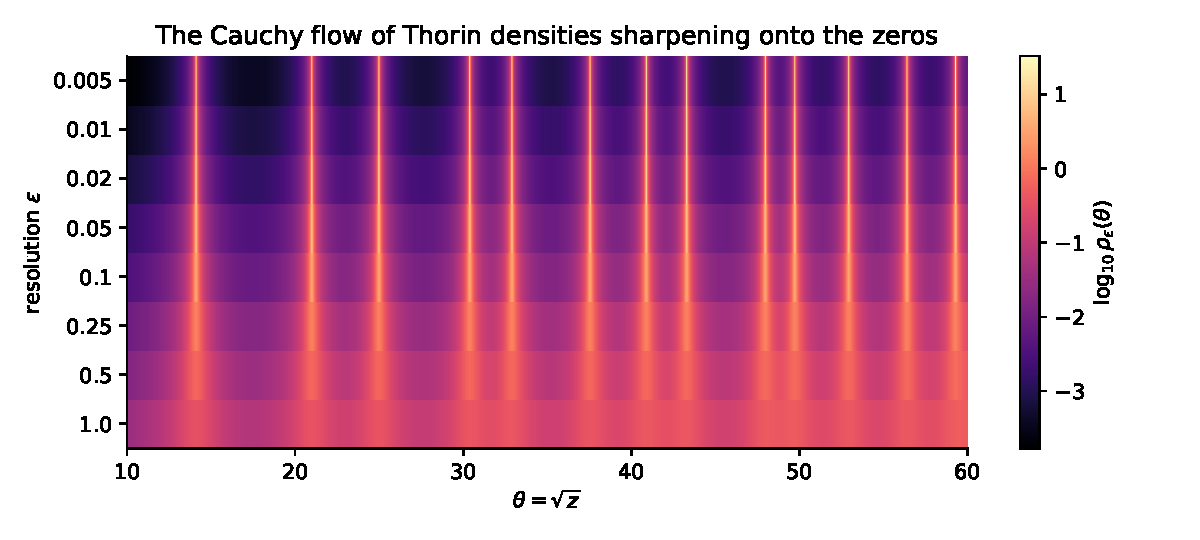
\includegraphics[width=\textwidth]{fig/flow.pdf}
\caption{The Thorin density $\rho_\varepsilon(\theta)$ on $10\le\theta\le60$, computed from the P\'olya density at eight resolutions from $\varepsilon=1$ (bottom) to $\varepsilon=0.005$ (top), on a logarithmic colour scale. As the resolution sharpens, the density concentrates on bright vertical lines at the ordinates of the zeros, all of which lie on the critical line in this window: the Cauchy flow converging to the RH measure $\sum\delta_{\gamma^2}$.}
\label{fig:ch1:flow}
\end{figure}

\subsection{Plan of the book and its principal results}

Two ideas set out in Sections~\ref{ch:clock} and \ref{ch:ggc} carry the rest of the book. The first, stated above, is that the Thorin measure at resolution $\varepsilon$ is the Poisson smoothing of the zeros and so is computable from any evaluator of $\xi$ off the critical line; as $\varepsilon\downarrow0$ it converges to the atoms on the line. The second is that the hierarchy of infinitely divisible laws becomes a hierarchy of positivity conditions on one function, the heat trace, of which the lower rungs are theorems and the top rung is RH. Every later chapter computes, tests or interprets one of these two ideas.

Chapter~\ref{chap:evaluation} evaluates $\xi$ and $\xi'$ in the complex plane by the P\'olya route, compares it with the classical evaluators and Turing's method, and follows one small computation from the theta series to a Thorin mass and a zero. Chapters~\ref{chap:measure} to \ref{chap:heat} are the core of the book. Chapter~\ref{chap:measure} measures the distance from the computed Thorin measure to $U_{\RH}$, computes the signature of an off line zero, reads the zero count and the zero density from the Thorin mass, and gives further readings of the sine squared lemma. Chapter~\ref{chap:hcm} treats weak convergence and hyperbolic complete monotonicity, brings in Bosch's theorem on powers of the half Cauchy law, and proves a theorem of the same shape for the clock, with a threshold set by the angle of the zeros. Chapter~\ref{chap:heat} climbs the hierarchy of positivity on the heat trace, explains what finite information cannot decide, computes the Thorin functional from the primes and relates the cell distance of Section~\ref{ch:distances} to the spacings of the zeros.

Chapters~\ref{chap:rzeta} and \ref{chap:rzid} study the reciprocal zeta function in the variable $u$ of the clock. The first gives its Thorin type forms and treats the gamma factor, the Meixner law and the sine squared lemma; the second proves that the normalised reciprocal zeta function is infinitely divisible and places it in the Bondesson hierarchy, then truncates the representation, due to Biane, Pitman and Yor, of $\xi$ as the Mellin transform of a GGC with Thorin atoms on a quadratic lattice and studies the conditions on the zeros of the truncations that would imply RH. Chapter~\ref{chap:probability}, with the P\'olya route as its evaluator, treats the clock as a random variable, through its law, its Kent approximants and its Brownian boundaries; it then turns to criteria other than the Thorin condition, the Keiper Li coefficients and the de Bruijn Newman flow, carries the evaluator to the $L$ functions of the character $\chi_{12}$, whose theta series is the Dedekind eta function, and of Ramanujan's $\Delta$, and recovers the zeros from the Thorin density by nonnegative deconvolution.

Chapters~\ref{chap:basepoint} to \ref{chap:almost} move the basepoint. The shifted clock $T_\alpha$ has Laplace transform $\xi(\alpha)/\xi(\alpha+\sqrt u)$; at $\alpha=\frac12$ it is the clock, and from $\alpha=1$ on its Thorin measure is positive with no hypothesis. These chapters carry both ideas from the basepoint one, the resolution $\varepsilon=\frac12$, into the critical strip. Chapter~\ref{chap:basepoint} works out the basepoint one, from the Mellin side, where $2\xi$ is a moment function of Bessel hitting times, to the Thorin measure and the law of $T_1$, and constructs $T_\alpha$ as a hitting time at every basepoint $\alpha>\frac12$. Chapter~\ref{chap:strip} extends the hierarchy to symmetric laws on the line, where the reciprocal of $\xi$ on the real axis is the characteristic function of a normal scale mixture, reads zero free half planes as completeness statements after Wiener, Salem and Riesz, and writes Riesz's criterion as the statement that every $T_\alpha$ with $\alpha>\frac12$ is a GGC. Chapter~\ref{chap:almost} reads the hierarchy through the books of Sato and Bondesson, repeats the calculations at the basepoint one for $L(s,\chi_{12})$, uses zero density estimates to bound how far each $T_\alpha$ can be from a GGC, and closes with the work of Anthony Pakes on size biasing, the Lambert law and ladders of self decomposable laws.

Chapter~\ref{chap:conclusions} assembles the results of the preceding chapters into a path towards RH on which every step is marked proved, computed, announced or open, sets out the computations that remain as one programme with its milestones, and draws the lessons of the computations for the Thorin programme. Chapter~\ref{chap:ferro} reads RH as a statement about one law, that the P\'olya variable is ferromagnetic, in the sense that its moment generating function vanishes only on the imaginary axis; it develops the class of such laws, checks the necessary conditions on the P\'olya law, builds, with no hypothesis, provably ferromagnetic laws within total variation distance $1.3\times10^{-4}$ of it and, by a computer assisted proof, within $2\times10^{-6}$, and shows that $e^{2X}$, a size biased form of the variable of Biane, Pitman and Yor, is self decomposable but not a generalised gamma convolution. Chapter~\ref{chap:maxwald} reads the P\'olya density as the density of a maximum order statistic of independent exponential variables and follows the clock through that representation: its Wald couple with the P\'olya variable, a criterion for the Thorin condition, an explicit generalised gamma convolution within a certified Laplace distance of it, the finite stages of the maximum and the Bondesson classes. Chapter~\ref{chap:phase} places the computations of the book on the Thorin phase diagram of the de Bruijn Newman flow, the set of points $(t,\alpha)$ at which the shifted clock of $\xi_t$ is a generalised gamma convolution, over which the minimum of $t+2(\alpha-\frac12)^2$ is the de Bruijn Newman constant, and certifies the finite part of one of its points below height $160$. Appendix~\ref{app:code} describes the code, the scripts and the data files behind the tables and figures, Appendix~\ref{app:history} gives a short history of computations on the zeros, Appendix~\ref{app:notation} lists the notation, and Appendix~\ref{app:bosch} gives the verification code for the Bosch type theorem.

Tables~\ref{tab:intro:summary}, \ref{tab:intro:summary45} and \ref{tab:intro:summary6} collect the principal results of Chapters~\ref{chap:evaluation} to \ref{chap:almost}, each with the section where it is developed. A result is marked proved when that section proves it or cites a proof, and computed when it rests on a computation; the section states how far the computation is certified.

{\footnotesize
\begin{longtable}{p{0.60\textwidth}p{0.12\textwidth}p{0.17\textwidth}}
\toprule
Result & Status & Where\\
\midrule
\endfirsthead
\toprule
Result & Status & Where\\
\midrule
\endhead
\bottomrule
\endfoot
\bottomrule
\caption{Principal results of Chapters~\ref{chap:evaluation} to \ref{chap:heat}.}\label{tab:intro:summary}\\
\endlastfoot
P\'olya route: $\xi$ and $\xi'$ from two fixed polynomials in ball arithmetic, about $60$ correct digits at height $200$ at $420$ bits, $0.7$ ms per point & \raggedright computed & Section~\ref{ch:polya}\\
Tilted contour: $25$ digits of $\rho_{0.05}$ at height $5000$ against \texttt{mpmath}, in $28$ ms per point; to leading exponential order the loss to cancellation falls from about $0.341\,\theta$ digits to about $\delta\theta/\log10$ & \raggedright proved and computed & Section~\ref{ch:polya}\\
The Lehmer pair near height $7005$ resolved by the tilted P\'olya route at $34$ ms per point & \raggedright computed & Section~\ref{sec:ch5:lehmer}\\
$N(1000)=649$ from the Thorin mass at resolution $\frac12$ and the argument along a horizontal segment & \raggedright computed & Section~\ref{sec:ch5:count}\\
Raw total variation to $U_{\RH}$ maximal; matched total variation at the floor $3.7\times10^{-9}\varepsilon$ of the tail model; cell distance $5.44\,\varepsilon$ & \raggedright computed & Section~\ref{ch:distances}\\
Mass defect $-(\varepsilon/\pi)\Xi'(\Theta)/\Xi(\Theta)$ to first order; at $\Theta=200$ the observed slope agrees with it to five digits at $\varepsilon=0.005$ & \raggedright proved and computed & Section~\ref{ch:distances}\\
Signatures of an off line pair in total variation and negative mass, exact for an omitted pair and for the negative mass, to leading order for a displaced pair & \raggedright proved & Section~\ref{ch:offline}\\
Zero density $\nu(\frac12+\varepsilon,200)=0$ at eight resolutions, from the argument principle identity of Proposition~\ref{prop:zerodensity} & \raggedright computed & Section~\ref{ch:turing}\\
Prime side of the sine squared lemma: when no zero has real part greater than $\frac12$, Selberg's smoothed sum computes $\rho_\varepsilon$ with relative error at most $(x^{-\varepsilon}+x^{-2\varepsilon})/(\varepsilon\log x)$, so with error of order $x^{-\varepsilon}/(\varepsilon^2\log x)$ at the peaks, the single zero law; tested at $\varepsilon=\frac14$ & \raggedright proved and computed & Section~\ref{ch:sin2more}\\
The Thorin measures converge vaguely to the measure of the zeros on the line, whether or not RH holds & \raggedright proved & Section~\ref{ch:weak}\\
The clock is HCM if and only if RH holds, and the shifted clock at any basepoint $\alpha\ge1$ is HCM unconditionally; the $216$ normalised derivatives of a finite HCM test are all positive, certified in ball arithmetic & \raggedright proved and computed & Section~\ref{ch:weak}\\
Bosch type threshold: $1/G(x^{1/\beta})$ is HCM if and only if $|\beta|\ge1/(1-\alpha_\xi)$, with $\alpha_\xi$ set by the largest angle of the zeros; unconditionally $1/G(x^p)$ is HCM for $|p|\le1-1/(\pi T_0)$, where $T_0=3\times10^{12}$ is the verified height, in particular for $|p|\le1-1.1\times10^{-13}$ & \raggedright proved & Section~\ref{ch:boschB}\\
The clock is infinitely divisible and self decomposable with no hypothesis, and $(-1)^kW^{(k)}>0$ for every $k\le1.16\times10^{25}$, that is, the Williamson measures, inverse gamma smoothings of the Thorin measure, are positive to that order; the two proofs use the verification of RH below heights $1000$ and $3\times10^{12}$ respectively \cite{PT21}; Laplace's method on the Gumbel tail of the P\'olya kernel and a Tauberian argument give the leading term of the Weyl law & \raggedright proved & Section~\ref{ch:heat}\\
\end{longtable}}

{\footnotesize
\begin{longtable}{p{0.60\textwidth}p{0.12\textwidth}p{0.17\textwidth}}
\toprule
Result & Status & Where\\
\midrule
\endfirsthead
\toprule
Result & Status & Where\\
\midrule
\endhead
\bottomrule
\endfoot
\bottomrule
\caption{Principal results of Chapters~\ref{chap:rzeta} to \ref{chap:probability}.}\label{tab:intro:summary45}\\
\endlastfoot
The normalised reciprocal zeta function is infinitely divisible with no hypothesis, and it is not self decomposable, not a GGC and not in the Bondesson class & \raggedright proved and computed & Section~\ref{ch:rz3}\\
Conjecture S, that the symmetrised truncations of the Biane, Pitman and Yor lattice have their zeros in the strip on the line, holds for the sizes $n\le24$ and $n=32,36$ above explicit heights and numerically below them; for infinitely many $n$ it would imply RH & \raggedright proved and computed & Section~\ref{ch:rz4}\\
Law of the clock by Talbot inversion, with no zero as input; its hazard tends to $\gamma_1^2$, reached to eleven digits at $t=0.25$ & \raggedright computed & Section~\ref{ch:clocklaw}\\
Kent approximants with $1700$ zeros and a moment matched Weyl tail: relative error $3.5\times10^{-23}$ at $u=1$ and $7.0\times10^{-13}$ at $u=10^4$; for large $u$ the error of the plain Weyl tail levels off at a constant set by $S$ & \raggedright computed & Section~\ref{ch:clocklaw}\\
The clock is not the first passage time of Brownian motion to an independent random level; the boundary from the Volterra equation, solved in three zones, reproduces its law to Monte Carlo accuracy (Kolmogorov distance $0.0020$, against $0.0059$ for the tangent boundary) & \raggedright proved and computed & Section~\ref{ch:boundaries}\\
Keiper Li coefficients $\lambda_1,\dots,\lambda_{100}$ from the P\'olya density, $\lambda_1$ to $25$ digits & \raggedright computed & Section~\ref{ch:li}\\
Closest pair below height $200$ collides at de Bruijn Newman time $-0.288$; the Lehmer pair near $7005$ at $-7.11\times10^{-4}$ & \raggedright computed & Section~\ref{ch:dbn}\\
For $L(s,\chi_{12})$ and $L(s,\Delta)$ the sine squared lemma has no pole piece but a signed prime piece & \raggedright proved & Section~\ref{ch:chi12}\\
The eta kernel of $L(s,\chi_{12})$: GRH below height $100$ from the zero density identity and the $67$ sign changes & \raggedright computed & Section~\ref{ch:chi12}\\
For an imaginary quadratic field the P\'olya kernel of $\zeta_K$ is positive exactly when an explicit theta sum is positive on a finite interval, which gives $L(\frac12,\chi_d)>0$ for $d=-3,-4,-7,-8$; it takes negative values for every $d\equiv5\pmod{24}$ & \raggedright proved & Section~\ref{ch:chi12}\\
For the Dirichlet beta function $L(s,\chi_4)$, whose kernel is the cube of the eta function: GRH below height $100$; a positive Thorin density at every basepoint $\alpha\ge1$, which the absolute values of the prime weights certify only for $\alpha>2.2823$; the density as the difference of those of $\xi_{\mathbb Q(i)}$ and $\xi$, and as the derivative of the argument of the completed function on the line & \raggedright proved and computed & Section~\ref{sec:dbeta:beta}\\
Nonnegative deconvolution of $\rho_{0.1}$ on $[15,55]$, with the zeros outside $[5,65]$ as background, recovers every zero in the window to within $10^{-5}$ & \raggedright computed & Section~\ref{ch:deconv}\\
For P\'olya's Bessel function $K_{i\theta/2}(2\pi)$ the index side clock is the hitting time of an explicit diffusion, its Thorin atoms are the squared zeros and its trace is completely monotone; its de Bruijn Newman constant is finite, by Newman's theorem, although none of its real zeros below height $90$ collide down to $t=-60$ & \raggedright proved and computed & Section~\ref{ch:biane}\\
\end{longtable}}

{\footnotesize
\begin{longtable}{p{0.60\textwidth}p{0.12\textwidth}p{0.17\textwidth}}
\toprule
Result & Status & Where\\
\midrule
\endfirsthead
\toprule
Result & Status & Where\\
\midrule
\endhead
\bottomrule
\endfoot
\bottomrule
\caption{Principal results of Chapters~\ref{chap:basepoint} to \ref{chap:almost}. All are unconditional, and several use verified computations: the verification of RH below height $1000$, through Theorem~\ref{thm:ch12:idsd}, or below the height $T_0=3\times10^{12}$, Platt's verification of GRH for small moduli, or computations in ball arithmetic.}\label{tab:intro:summary6}\\
\endlastfoot
$T_1$, with Laplace transform $\xi(1)/\xi(1+\sqrt u)$, is a GGC with positive Thorin density, smallest at the origin, by a computation of the zeros below height $2000$ in ball arithmetic and explicit zero counts above it, so that $T_1$ is a positive stable one half variable plus an independent GGC; its law has infinite mean and a stable one half tail, and the L\'evy form of $\xi(1+s)$, which converges by the prime number theorem, gives its Thorin density from the primes & \raggedright proved and computed & Section~\ref{ch:basepoint}\\
Below the basepoint one, $v_\alpha(\theta)/(\alpha-\frac12)$ is nonincreasing in $\alpha$ away from the zeros off the line; the Thorin density is smallest at the origin, and only there, for every $\alpha\in(\frac12,7.35]$ on $|\theta|\le3\times10^{12}-1.21$, for $L(s,\chi_4)$ and $L(s,\chi_{12})$ at every height for every $\alpha\ge1$, and at every height for every $\alpha\in(\frac12,1)$ exactly when RH holds; for every $\alpha>\frac12$ it is positive on $|\theta|\le3\times10^{12}-\frac12$ & \raggedright proved and computed & Sections~\ref{sec:dbeta:comp}, \ref{ch:almost}\\
Every $T_\alpha$, $\alpha>\frac12$, exists as the tilted centre clock run through the inverse local time of a sticky Brownian motion, and it is a GGC if and only if no zero has real part greater than $\alpha$ & \raggedright proved & Section~\ref{ch:bphit}\\
For real $u$ and $\alpha\ge\frac12$, $\xi(\alpha)/\xi(\alpha+|u|)$ is the characteristic function of an infinitely divisible normal scale mixture; for $\frac12<\alpha<1$ it is an extended GGC, and the translates of every tilted P\'olya kernel $\Phi_{\alpha'}$ with $\alpha'>\alpha$ are complete in $L^1$, exactly when no zero has real part greater than $\alpha$ & \raggedright proved & Section~\ref{ch:strip}\\
The complete monotonicity conditions of the Poisson trace $K_{1/2}$, which together are RH, hold for every order $n<T_0(\pi-y)$ at the point $y$; $K_{1/2}$ and the trace of P\'olya's Bessel function differ by $\frac98+O(y\log\frac1y)$ as $y\to0$ & \raggedright proved and computed & Section~\ref{sec:biane:cm}\\
$1/\zeta(2k)$ is, up to an elementary factor, a value of the Laplace transform of the centre clock and of $T_1$; for $\frac12\le\alpha<1$ the bound $O(x^{\alpha/2+\delta})$ on Riesz's function, for every $\delta>0$, holds exactly when every $T_{\alpha'}$ with $\alpha'>\alpha$ is a GGC & \raggedright proved & Section~\ref{ch:riesz}\\
The constant of $\sum_{n\le x}\mu(n)^2/n$ is an elementary term plus $\E V_1-2\,\E V_2$, two tilted P\'olya means; RH holds exactly when the squarefree count smoothed by an exponential or a Gamma(2) law, or the count in mean square, has error $O(x^{1/4+\varepsilon})$; the error is $\Omega_\pm(x^{1/4})$; Gamma(2) smoothing writes it as an average of the Mertens function under a positive law, and two is the largest shape for which this holds & \raggedright proved & Section~\ref{sec:sqfree}\\
The centre clock is driven by a subordinator with L\'evy density $-W'$ and is unimodal, as is $T_\alpha$ for $\alpha\ge1$; the tilted P\'olya variable is quasi infinitely divisible for every $\alpha>1$ but not at $\alpha=1$ & \raggedright proved & Section~\ref{ch:sato}\\
For $L(s,\chi_{12})$ the Thorin measure at the basepoint one is positive, and its L\'evy form there has no pole to compensate and prime atoms of both signs & \raggedright proved & Section~\ref{ch:bpeta}\\
For $\frac12<\alpha<1$, in the density $\rho_{\alpha-1/2}$ the Cauchy kernels of the zeros to the right of $\alpha$ carry at heights $\theta\le T$ at most $T^{e(\alpha)-1+o(1)}$ times the mass of the kernels of the other zeros, with $e(\alpha)<1$, by the zero density estimates of Ingham, of Guth and Maynard and of Huxley \cite{Ingham40,GM26,Huxley72} & \raggedright proved & Section~\ref{ch:almost}\\
With no hypothesis, the size biased centre clock is the clock plus an independent variable with density $W/\E T$, and RH holds exactly when this variable is a mixture of exponential laws, with weight $\gamma^{-2}/\E T$ at the rate $\gamma^2$, about a fifth at the lowest zero; the Lambert law, with Laplace transform $\mathcal W(u)/u$, is a GGC whose Thorin measure is the image of the uniform law on $(0,\pi)$ under $b\mapsto b\,e^{-b\cot b}/\sin b$, by a proof of which only one step fails for the clock, and that step is RH & \raggedright proved and computed & Sections~\ref{pk:sec:form}, \ref{pk:sec:lambert}\\
The centre clock lies in Urbanik's class $L_2$ of multiply self decomposable laws and not in $L_3$; it is not the martingale limit of a supercritical continuous state branching process with finite Malthusian parameter & \raggedright proved and computed & Section~\ref{pk:sec:ladder}\\
A property of even kernels that also holds for the damped P\'olya kernel $e^{tv^2/4}\Phi(v)$ for some $t<0$ cannot by itself imply RH, by the theorem of Rodgers and Tao; the GGC property of the variable of Biane, Pitman and Yor fails for the damped kernel at every $t<0$ tested and, provably, for small $|t|$, so the filter does not exclude it there & \raggedright proved and computed & Section~\ref{pk:sec:filter}\\
\end{longtable}}

\subsection{Conventions and how to read this book}

The clock is a function of $u=s^2$, so that the atoms of its Thorin measure are at $\gamma^2$; earlier papers of the programme used $s^2/2$, which rescales Thorin measures by $z\mapsto z/2$. Thorin measures are measures in the variable $z$, and we write $\theta=\sqrt z$ for the chart in which the Thorin measure at the basepoint $\frac12+\varepsilon$ has density $\rho_\varepsilon(\theta)=\pi^{-1}\re(\xi'/\xi)(\frac12+\varepsilon+i\theta)$; $\varepsilon$ is the resolution. The P\'olya kernel $\Phi$ is taken in Titchmarsh's normalisation, $\Xi(\theta)=\int_{\mathbb R}\Phi(u)\cos(\theta u)\,du$. $N(T)$ counts zeros with $0<\im\rho\le T$ and $\nu(\sigma,T)$ those with, in addition, $\re\rho>\sigma$. Total variation of a signed measure is the total variation norm $|\mu|(E)$ on the stated window. Chapters~\ref{chap:rzeta} and \ref{chap:rzid}, and Sections~\ref{ch:boschA} and \ref{ch:boschB}, write $s$ for $u$, and the Kent approximants of Section~\ref{ch:clocklaw} write $w$; each declares its variables where it starts, and Appendix~\ref{app:notation} lists the notation of the book with the place where each symbol is defined. Numerical values are quoted to the accuracy at which they have been checked, and the section in which a value is computed says how.

Readers mainly interested in computation can read Sections~\ref{ch:clock}, \ref{ch:polya} and \ref{ch:worked} and then go straight to Chapters~\ref{chap:measure} to \ref{chap:heat}, where the Thorin condition is analysed numerically. Readers interested in the probabilistic side can start with Sections~\ref{ch:ggc}, \ref{ch:clocklaw} and \ref{ch:boundaries} and continue with Chapters~\ref{chap:basepoint} to \ref{chap:almost}, where the shifted clocks are hitting times and normal scale mixtures; these chapters build on Sections~\ref{ch:clock} and \ref{ch:ggc} and draw on Section~\ref{ch:turing} for the zero count. Chapters~\ref{chap:rzeta} and \ref{chap:rzid} can be read after Chapter~\ref{chap:foundations} and the statements of Theorems~\ref{thm:ch12:idsd} and \ref{thm:ch12:cm} in Section~\ref{ch:heat}; they form the most technical part of the book, and they prove unconditional theorems about the reciprocal zeta function. Readers looking for the conclusions can go directly to Sections~\ref{ch:path} and \ref{ch:lessons}. Throughout, statements are marked as proved, computed, announced or open, and Appendix~\ref{app:code} names the script behind each computed table and figure or records that the archive has none.

\section{The Xi function, the P\'olya density and the clock}\label{ch:clock}
\label{sec:clock}

Section~\ref{ch:intro} states RH as a positivity condition on the clock $1/G$, and computation with that condition rests on four objects. The Hadamard product of $\xi$ in the variable $u=s^2$ turns RH into a statement about the zeros of an entire function of genus zero. The P\'olya kernel makes $\xi(\frac12+s)/\xi(\frac12)$ the moment generating function of a probability density, and it underlies the evaluator of Section~\ref{ch:polya}. The heat trace of the zeros turns the classes of infinitely divisible laws into sign conditions on a single function, and the explicit formula expresses it through the primes. At the basepoint $\frac12+\varepsilon$ the Thorin density is the Poisson smoothing of the zeros at every resolution $\varepsilon>0$, and it is the density of the Thorin measure of a GGC when the basepoint lies to the right of every zero; the sine squared lemma produces the same density from the primes. The rest of the book computes these objects and measures how close they come to the discrete measure that RH demands. Most of the material is classical or taken from \cite{P26}.

\subsection{The completed zeta function and the clock}

The completed zeta function $\xi$ of Section~\ref{ch:intro} is entire of order one and maximal type, satisfies $\xi(s)=\xi(1-s)$ and $\overline{\xi(\bar s)}=\xi(s)$, and is positive on the real axis. On the critical line $\Xi(\theta)=\xi(\frac12+i\theta)$ is real and even. The zeros $\rho=\beta+i\gamma$ of $\xi$ lie in the open strip $0<\re s<1$ and are symmetric under $\rho\mapsto1-\rho$ and $\rho\mapsto\bar\rho$. As in Section~\ref{ch:intro}, $G(u)=\xi(\frac12+\sqrt u)/\xi(\frac12)$, and $a_k=-(\rho_k-\frac12)^2$, one for each pair $\{\rho,1-\rho\}$.

Hadamard's theorem applied to $G$, which is entire of order $\frac12$, gives, with $u=s^2$,
\begin{equation}\label{eq:ch2:hadamard}
\frac{\xi(\frac12+s)}{\xi(\frac12)}=\prod_k\Big(1-\frac{s^2}{(\rho_k-\frac12)^2}\Big)=\prod_k\Big(1+\frac{s^2}{a_k}\Big),
\end{equation}
with $\sum|a_k|^{-1}<\infty$. Logarithmic differentiation gives the partial fraction expansion
\begin{equation}\label{eq:ch2:partial}
\frac{\xi'}{\xi}(s)=\sum_\rho\frac1{s-\rho},
\end{equation}
in which each $\rho$ is grouped with $1-\rho$, as the differentiation of \eqref{eq:ch2:hadamard} produces, or with $\bar\rho$. Grouped either way the series converges absolutely, since each group is $O(\gamma^{-2})$ for fixed $s$ and $\sum_\rho\gamma^{-2}<\infty$; without grouping it converges only when summed symmetrically in $\im\rho$. Its real part $\sum_\rho\re(s-\rho)/|s-\rho|^2$ converges absolutely without grouping.

Passing to $u=s^2$ folds each pair $\pm(\rho_k-\frac12)$ of zeros of $\xi(\frac12+s)$ into the single zero $-a_k$ of $G$, so the product has genus zero and needs no exponential factors. Since $\xi$ has no real zeros, $a_k$ is real only when $\rho_k$ lies on the critical line, and then $a_k=\gamma_k^2>0$. RH is therefore the statement that every zero of $G$ lies on the negative real axis. The reciprocal of a product of genus zero with negative zeros is a product of gamma Laplace transforms, and this is how generalised gamma convolutions enter.

A random variable $H\ge0$ is a generalised gamma convolution (GGC) if $\E e^{-uH}=\exp\{-du-\int_{(0,\infty)}\log(1+u/z)\,U(dz)\}$ for $u>0$, with a drift $d\ge0$ and a positive measure $U$, the Thorin measure, such that $\int_{(0,1)}|\log z|\,U(dz)+\int_{(1,\infty)}z^{-1}U(dz)<\infty$. The drift and the Thorin measure are unique, and the Laplace transform of a GGC extends to a holomorphic nonvanishing function on $\cut$. Section~\ref{ch:ggc} develops the class from the same definition, \eqref{eq:ch3:ggc}.

Unconditionally, $1/G$ is the Laplace transform of a probability law on $[0,\infty)$ \cite[Theorem A]{P26}; Section~\ref{ch:heat} states this as Theorem~\ref{thm:ch12:idsd} and proves it. A random variable $T$ with $\E e^{-uT}=1/G(u)$ for $u\ge0$ is called the clock variable. Its mean and variance are $\E T=\sum_ka_k^{-1}=G'(0)=\xi''(\frac12)/(2\xi(\frac12))=0.0231050$ and $\operatorname{Var}T=\sum_ka_k^{-2}=3.71726\times10^{-5}$; these constants, and $\xi(\frac12)=0.4971207781883141$, recur throughout the book. The Thorin condition asks whether $T$ is a GGC, and the answer is the rigidity theorem stated in Section~\ref{ch:intro}, which we restate with its source.

\begin{proposition}[Rigidity, {\cite[Proposition 3.4]{P26}}]\label{prop:rigid}
The clock $1/G$ is the Laplace transform of a GGC if and only if RH holds, and then its Thorin measure is $U_{\RH}$ of \eqref{eq:URH} and the clock variable is $T=\sum_{\gamma>0}e_\gamma/\gamma^2$ with independent standard exponentials $e_\gamma$.
\end{proposition}

The name refers to the absence of any freedom in the Thorin measure. If $1/G$ is the Laplace transform of a GGC with drift $d$ and Thorin measure $U$, then $d+\int U(dz)/(u+z)=G'/G(u)=\sum_k(u+a_k)^{-1}$ for $u>0$. The left side is holomorphic on $\cut$, so every pole $-a_k$ of the right side lies on the negative real axis. Hence every $a_k$ is positive, which is RH, and uniqueness of the Stieltjes representation forces $d=0$ and $U=\sum_k\delta_{a_k}$. Conversely, under RH, \eqref{eq:ch2:hadamard} writes $1/G$ as a product of gamma Laplace transforms.

\subsection{The P\'olya kernel and the P\'olya density}

Riemann's continuation of $\zeta$ writes $\xi$ as a Mellin transform of a combination of $\omega(x)=\sum_{n\ge1}e^{-\pi n^2x}$ and its derivatives, and uses the theta transformation $1+2\omega(1/x)=\sqrt x\,(1+2\omega(x))$, $x>0$. The substitution $x=e^{2u}$ turns the Mellin transform into a Fourier transform, and in Titchmarsh's normalisation \cite[Section 10.1]{Titchmarsh} the result is
\begin{equation}\label{eq:ch2:Phi}
\begin{aligned}
\Phi(u)&=2\sum_{n\ge1}\big(2\pi^2n^4e^{9u/2}-3\pi n^2e^{5u/2}\big)\exp(-\pi n^2e^{2u}),\\
\Xi(\theta)&=\int_{\mathbb R}\Phi(u)\cos(\theta u)\,du .
\end{aligned}
\end{equation}
Here $u$ is the variable of the kernel, not the argument of the clock. P\'olya studied this representation \cite{Polya}, and $\Phi$ is called the P\'olya kernel.

The kernel is even and strictly positive, and $\Phi(u)\sim4\pi^2e^{9|u|/2}\exp(-\pi e^{2|u|})$ as $|u|\to\infty$. Evenness is the functional equation read through the theta transformation (Exercise~\ref{ex:ch2:even}). For $u\ge0$ every term of \eqref{eq:ch2:Phi} is positive, because $2\pi^2n^4e^{9u/2}-3\pi n^2e^{5u/2}=\pi n^2e^{5u/2}(2\pi n^2e^{2u}-3)$ and $2\pi n^2e^{2u}\ge2\pi>3$; positivity for $u<0$ follows by evenness. Evenness also decides how $\Phi$ is computed. Term $n$ is $n^{-1/2}$ times the first term translated to the left by $\log n$, so for $u\ge0$ the first term dominates, while for $u<0$ the terms are individually of order $n^{-1/2}$ and cancel almost completely. The theta transformation turns their sum into the mirror image of the side $u>0$, and computations therefore evaluate $\Phi(|u|)$.

Each term of \eqref{eq:ch2:Phi} is entire in $u$, and since $\re e^{2u}=e^{2x}\cos2y$ for $u=x+iy$, the series converges locally uniformly in the strip $|\im u|<\pi/4$, so $\Phi$ is analytic there; the boundary lines $\im u=\pm\pi/4$ are a natural boundary inherited from the theta function \cite[Chapter 11, Section 1.4, and Chapter 5, Section 3.2]{Remmert98}. The strip of analyticity makes the trapezoid rule spectrally accurate and permits the tilted contour of Section~\ref{sec:newcomp}. Figure~\ref{fig:ch2:kernel} shows $|\Phi|$ on lines inside the strip.

\begin{figure}[htbp]
\centering
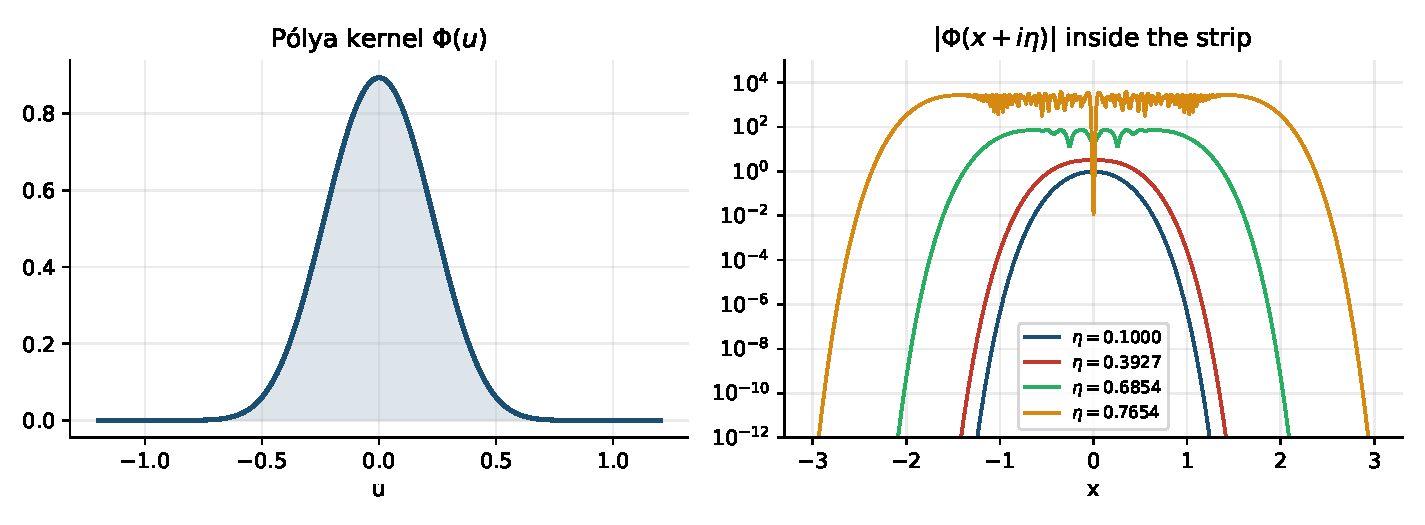
\includegraphics[width=\textwidth]{fig/kernel.pdf}
\caption{Left: the P\'olya kernel $\Phi(u)$ on the real line. Right: $|\Phi(x+i\eta)|$, on a logarithmic scale, on the lines $\eta=0.1000$, $0.3927$, $0.6854$ and $0.7654$ inside the strip of analyticity, that is at distances $0.6854$, $0.3927$, $0.1$ and $0.02$ below its edge $\eta=\pi/4$ (the tilts of Section~\ref{sec:newcomp}). As the line approaches the natural boundary $\eta=\pi/4$ the kernel grows and spreads (compare Table~\ref{tab:ch4:Meta}), and it still decays doubly exponentially in $|x|$.}
\label{fig:ch2:kernel}
\end{figure}

Since $\Xi(0)=\xi(\frac12)=\int_{\R}\Phi$, the P\'olya density $p=\Phi/\Xi(0)$ is the law of a symmetric random variable $X$ with all exponential moments, and
\begin{equation}\label{eq:ch2:mgf}
\frac{\xi(\frac12+s)}{\xi(\frac12)}=\E\,e^{sX}=\E\cosh(sX),\qquad s\in\C .
\end{equation}
The zeros of $\xi(\frac12+s)$ are therefore the complex $s$ at which the moment generating function of $X$ vanishes, and the ordinates of the zeros on the critical line are the real zeros of its characteristic function $\E\cos(\theta X)$. The clock is $1/\E\cosh(\sqrt u\,X)$, and at $u=\theta^2$ it forms with the characteristic function of $X$ a van Dantzig pair, that is, a pair $(\varphi_1,\varphi_2)$ of characteristic functions with $\varphi_2(\theta)=1/\varphi_1(i\theta)$; the name goes back to a problem of van Dantzig, which Lukacs studied \cite{Lukacs68}. Here $\varphi_1(\theta)=\Xi(\theta)/\Xi(0)$ is the characteristic function of $X$, and $1/\varphi_1(i\theta)=\xi(\frac12)/\xi(\frac12+\theta)=\E e^{-\theta^2T}$ is the characteristic function of $Z\sqrt{2T}$, with $Z$ standard normal and independent of $T$ \cite[Theorem A]{P26}. G.~Letac asked whether $\varphi_1$ is the first member of a van Dantzig pair (private communication), and Theorem~\ref{thm:ch12:idsd} shows that it is, unconditionally. Section~\ref{ch:strip} reads the reciprocal of $\xi$ along the real axis in the same way at every basepoint, and it shows by Wiener's closure theorem that the translates of $\Phi$ are not dense in $L^1(\R)$, because $\Xi$ has real zeros (Proposition~\ref{wr:prop:wiener}).

Two classical pairs show the shape to expect. The first is $(\cos\theta,1/\cosh\theta)$, the symmetric Bernoulli law on $\{-1,1\}$ with the hyperbolic secant law, and the second is $(\sin\theta/\theta,\theta/\sinh\theta)$, the uniform law on $[-1,1]$ with the logistic law scaled by $1/\pi$. In both the first member has only real zeros and the second is the product of the reciprocal factors: $1/\cosh\theta=\prod_{k\ge1}(1+\theta^2/((k-\frac12)\pi)^2)^{-1}$ is the characteristic function of $\sum_{k\ge1}L_k/((k-\frac12)\pi)$, where the $L_k$ are independent standard Laplace variables, with density $\frac12e^{-|x|}$ and characteristic function $1/(1+\theta^2)$, and likewise $\theta/\sinh\theta$ is that of $\sum_{k\ge1}L_k/(k\pi)$. The product form alone does not make a pair, since the first member must be a characteristic function in its own right, and $\prod_k(1-\theta^2/c_k^2)$ over finitely many real $c_k$ is an unbounded polynomial.

The Xi pair has the classical shape exactly when RH holds. If RH holds, $T=\sum_{\gamma>0}e_\gamma/\gamma^2$ (Proposition~\ref{prop:rigid}), and since $Z\sqrt{2e}$ is a standard Laplace variable when $e$ is a standard exponential variable independent of $Z$, $Z\sqrt{2T}$ has the law of $\sum_{\gamma>0}L_\gamma/\gamma$, the sum that Section~\ref{ch:boschA} calls $\log W$. Conversely, if $Z\sqrt{2T}$ has the law of $\sum_kL_k/c_k$ for real $c_k$ with $\sum_kc_k^{-2}<\infty$, then $\xi(\frac12+\theta)/\xi(\frac12)=\prod_k(1+\theta^2/c_k^2)$ for real $\theta$, hence for complex $\theta$, and every zero of $\xi$ lies on the critical line. Konstantopoulos, Patie and Sarkar state the same equivalence in the language of the Laguerre P\'olya class and of P\'olya frequency functions \cite[Theorem 2.3 and Corollary 2.4]{KPS24}. Table~\ref{tab:ch2:vd} computes the two members and compares them with their Hadamard products over the first $1700$ zeros, all of which lie on the line; the zeros above them enter through $\E T=\sum_ka_k^{-1}$ and $\operatorname{Var}T=\sum_ka_k^{-2}$, which are read off from the Taylor coefficients of $\log\xi(\frac12+s)$ at $s=0$ with no hypothesis on the zeros. Section~\ref{ch:strip} adds that the second member is self decomposable, that a zero off the line would contribute a factor that is not itself a characteristic function, and that away from the centre there is no such pair.

\begin{table}[htbp]
\centering\small
\begin{tabular}{rccc}
\toprule
$\theta$ & $\Xi(\theta)/\Xi(0)$ & $\xi(\frac12)/\xi(\frac12+\theta)$ & products, relative difference\\
\midrule
1 & 0.97714167 & 0.97717800 & $1\times10^{-18}$\\
2 & 0.91144824 & 0.91199057 & $8\times10^{-17}$\\
5 & 0.55429185 & 0.56739462 & $2\times10^{-14}$\\
10 & 0.076375505 & 0.11524595 & $1\times10^{-12}$\\
15 & $-1.4195704\times10^{-3}$ & $1.0310555\times10^{-2}$ & $1\times10^{-11}$\\
20 & $-7.3735457\times10^{-5}$ & $4.8509905\times10^{-4}$ & $8\times10^{-11}$\\
25 & $2.7809283\times10^{-8}$ & $1.3591692\times10^{-5}$ & $3\times10^{-10}$\\
30 & $-3.0207191\times10^{-8}$ & $2.4728825\times10^{-7}$ & $9\times10^{-10}$\\
\bottomrule
\end{tabular}
\caption{The van Dantzig pair, computed by \texttt{vdpair.py}. The last column is the larger relative difference between a member and its Hadamard product, $\prod(1-\theta^2/\gamma^2)$ or $\prod(1+\theta^2/\gamma^2)^{-1}$, over the $1700$ zeros below height $2198$, with the zeros above entering through $\sum_ka_k^{-1}$ and $\sum_ka_k^{-2}$; it is the size of the neglected term of order $\theta^6$. On $(0,30]$ the first member changes sign at $\gamma_1=14.13$, $\gamma_2=21.02$ and $\gamma_3=25.01$; the second is positive and decreasing. Both are $1-\theta^2\E T+O(\theta^4)$.}
\label{tab:ch2:vd}
\end{table}

The P\'olya variable also has a probabilistic construction. Let $S_2=\sum_{k\ge1}\frac2{\pi^2k^2}(e_k+e_k')$ with independent standard exponentials $e_k,e_k'$; it has the law of the sum of two independent hitting times of level $1$ by a three dimensional Bessel process started at $0$. By the theorem of Biane, Pitman and Yor \cite{BPY01}, going back to Williams \cite{Williams90}, $2\xi(s)=\E[(\pi S_2/2)^{s/2}]$. With $Y=\frac12\log(\pi S_2/2)$ this reads $\E e^{sY}=2\xi(s)$, so $X$ is $Y$ tilted by $e^{Y/2}$: $\E f(X)=\E[f(Y)e^{Y/2}]/\E e^{Y/2}$. Section~\ref{ch:clocklaw} uses this to estimate $\Xi$ from samples of $S_2$ and shows why sampling cannot locate the zeros. Tilting $Y$ by $e^{\alpha Y}$ in place of $e^{Y/2}$ gives, at every real basepoint $\alpha$ and with no hypothesis on the zeros, a variable $V_\alpha$ with $\E e^{sV_\alpha}=\xi(\alpha+s)/\xi(\alpha)$ and $V_{1/2}=X$ (Section~\ref{bp:sec:mellin}).

\subsection{The heat trace: spectral and arithmetic forms}

The heat trace of the zeros is
\[
W(t)=\sum_ke^{-a_kt}=\tfrac12\sum_\rho e^{(\rho-\frac12)^2t},\qquad t>0,
\]
and the series converges absolutely for every $t>0$ wherever the zeros lie, since $\re a_k=\gamma_k^2-(\beta_k-\frac12)^2>\gamma_k^2-\frac14$ for $\rho_k=\beta_k+i\gamma_k$. Integrating $e^{-(u+a_k)t}$ term by term, and using Frullani's integral $\log(1+u/a)=\int_0^\infty(1-e^{-ut})e^{-at}t^{-1}dt$ for $\re a>0$, gives, unconditionally for $u>0$ \cite[Theorem 4.3]{P26},
\[
\frac{G'}{G}(u)=\int_0^\infty e^{-ut}W(t)\,dt,\qquad \log G(u)=\int_0^\infty\big(1-e^{-ut}\big)\frac{W(t)}t\,dt .
\]
The second formula shows that $W(t)/t$ is the only possible L\'evy density of the clock variable $T$.

The classes of infinitely divisible laws of Section~\ref{sec:ch3:hierarchy} become sign conditions on $W$ \cite[Theorem 4.6]{P26}: $T$ is infinitely divisible if and only if $W\ge0$, self decomposable if and only if $W$ is nonincreasing, and a GGC if and only if $W$ is completely monotone, which by Proposition~\ref{prop:rigid} happens if and only if RH holds. The first two conditions hold unconditionally, in the strict forms $W>0$ and $W'<0$ on $(0,\infty)$ (Theorem~\ref{thm:ch12:idsd}, \cite[Theorem A]{P26}), by a proof that uses the verification of RH below height $1000$; the third is the Thorin condition, and Table~\ref{tab:ch3:hierarchy} records the rungs proved between them.

The explicit formula expresses $W$ through the primes. For even test functions $h$ holomorphic and rapidly decreasing in a strip $|\im r|\le\frac12+c$ with $c>0$, Weil's explicit formula \cite{Weil52}, \cite[Theorem 5.12]{IwaniecKowalski04}, reads
\begin{multline*}
\sum_\rho h(\gamma_\rho)=h(\tfrac i2)+h(-\tfrac i2)+\frac1{2\pi}\int_{\R}h(r)\big(\re\psi(\tfrac14+\tfrac{ir}2)-\log\pi\big)dr\\
-2\sum_{n\ge2}\frac{\Lambda(n)}{\sqrt n}\,g(\log n),
\end{multline*}
where $\rho=\frac12+i\gamma_\rho$, $g(x)=\frac1{2\pi}\int_{\R}h(r)e^{-irx}dr$ and $\psi=\Gamma'/\Gamma$ is the digamma function. The Gaussian $h(r)=e^{-r^2t}$ has $g(x)=e^{-x^2/4t}/(2\sqrt{\pi t})$ and $\sum_\rho h(\gamma_\rho)=2W(t)$, which gives the arithmetic form \cite[Theorem 4.4]{P26}
\begin{equation}\label{eq:ch2:Warith}
\begin{aligned}
W(t)&=e^{t/4}+\frac1{4\pi}\int_{\mathbb R}e^{-r^2t}m(r)\,dr-\frac1{2\sqrt{\pi t}}\sum_{n\ge2}\frac{\Lambda(n)}{\sqrt n}e^{-(\log n)^2/4t},\\
m(r)&=\re\psi\big(\tfrac14+\tfrac{ir}2\big)-\log\pi .
\end{aligned}
\end{equation}

The three terms of \eqref{eq:ch2:Warith} are the polar, archimedean and prime contributions. The polar term $e^{t/4}$ comes from $h(\pm\frac i2)$, that is, from the poles of $\pi^{-s/2}\Gamma(s/2)\zeta(s)$ at $s=1$ and $s=0$, which the factor $s(s-1)$ of $\xi$ removes. The archimedean term averages the digamma function of the gamma factor against a Gaussian and is negative for moderate $t$. The prime term is the series $\sum\Lambda(n)n^{-1/2}$ smoothed by a Gaussian of standard deviation $\sqrt{2t}$ in $\log n$: for small $t$ only the smallest primes contribute, and for large $t$ many primes contribute with nearly equal weight. As $t\to\infty$ the prime term grows like the polar term: $W(t)\to0$ and the archimedean term tends to $0$, so \eqref{eq:ch2:Warith} forces the prime term to be $e^{t/4}+o(1)$, and $W$ is what remains after the two cancel.

Table~\ref{tab:ch2:W} reproduces the comparison of \cite[Table 4.1]{P26}, and the two sides agree to fifteen digits. The polar and archimedean terms are of order one and the prime term rises from $8.4\times10^{-6}$ at $t=0.01$ to $0.30$ at $t=0.2$, while $W(t)$ decays like $e^{-\gamma_1^2t}$ with $\gamma_1^2=199.79$. An estimate of $W$ from \eqref{eq:ch2:Warith} at moderate $t$ must therefore survive a cancellation whose depth grows linearly in $t$. Section~\ref{sec:ch14:heat} extends the comparison to smaller and larger $t$ and gives that depth explicitly.

\begin{table}[htbp]
\centering\footnotesize\setlength{\tabcolsep}{4pt}
\begin{tabular}{@{}rllll@{}}
\toprule
$t$ & $W(t)$ from zeros & polar $+$ archimedean $-$ prime & archimedean & prime\\
\midrule
0.01 & 0.149698011253780 & 0.149698011253780 & $-0.8527967$ & $8.3995\times10^{-6}$\\
0.02 & $1.85412917313195\times10^{-2}$ & $1.85412917313195\times10^{-2}$ & $-0.9840612$ & 0.0024101\\
0.05 & $4.58783504857357\times10^{-5}$ & $4.58783504857357\times10^{-5}$ & $-0.9546186$ & 0.0579140\\
0.10 & $2.10479979582235\times10^{-9}$ & $2.10479979582235\times10^{-9}$ & $-0.8625096$ & 0.1628055\\
0.20 & $4.43018218022364\times10^{-18}$ & $4.43018218022364\times10^{-18}$ & $-0.7497538$ & 0.3015173\\
\bottomrule
\end{tabular}
\caption{The heat trace from the zeros and from the explicit formula, after \cite[Table 4.1]{P26}. At $t=1$ the cancellation between the arithmetic terms reaches about eighty seven digits.}
\label{tab:ch2:W}
\end{table}

\subsection{The Thorin density at a shifted basepoint}

Whether or not the Thorin condition holds at the centre, at a basepoint $\alpha$ to the right of every zero the shifted clock $u\mapsto\xi(\alpha)/\xi(\alpha+\sqrt u)$ is the Laplace transform of a GGC with an explicit Thorin density. The same formula defines a density at every basepoint $\alpha>\frac12$, whatever the zeros do, so it can be computed at every positive resolution $\alpha-\frac12$, and it is the starting point of the computations in Chapters~\ref{chap:measure} to \ref{chap:heat}. For a real basepoint $\alpha$ write $v_\alpha(r)=\re(\xi'/\xi)(\alpha+ir)$, and let $U_\alpha$ be the signed measure on $(0,\infty)$ given by
\begin{equation}\label{eq:Ualpha}
U_\alpha(dz)=\frac{v_\alpha(\sqrt z)}{2\pi\sqrt z}\,dz .
\end{equation}
At $\alpha=\frac12+\varepsilon$, where $\varepsilon>0$ is the resolution, the chart $\theta=\sqrt z$ gives $U_\alpha$ the density
\begin{equation}\label{eq:rho}
\rho_\varepsilon(\theta)=\frac1\pi\,v_{1/2+\varepsilon}(\theta)=\frac1\pi\re\frac{\xi'}{\xi}\Big(\frac12+\varepsilon+i\theta\Big),
\end{equation}
so that $U_\alpha(dz)=\rho_\varepsilon(\theta)\,d\theta$. The family $\varepsilon\mapsto\rho_\varepsilon$ is the Cauchy flow of \cite[Chapter 8]{P26}.

\begin{theorem}[{\cite[Theorem 3.7 and Remark 3.10]{P26}}]\label{thm:poisson}
If $\alpha>\re\rho$ for every zero, in particular for every $\alpha\ge1$, then $u\mapsto\xi(\alpha)/\xi(\alpha+\sqrt u)$ is the Laplace transform of a GGC $T_\alpha$ with Thorin density \eqref{eq:Ualpha}, and $v_\alpha>0$. It is the Laplace transform of a GGC if and only if $\alpha\ge\sup_\rho\re\rho$.
\end{theorem}

Since no zero lies on or to the right of the line $\re s=1$, the hypothesis of the theorem holds at $\alpha=1$, and Section~\ref{ch:basepoint} works out the shifted clock there in full. Until 2026 no smaller basepoint was known to satisfy it; the zero free half plane $\re s>\frac78$ announced in October 2026 would give every $\alpha>\frac78$ (Section~\ref{sec:ch25:open}). At every basepoint $\alpha>\frac12$ the shifted clock is still the Laplace transform of a probability law, with no hypothesis on the zeros (Theorem~\ref{bp:thm:alpha}); what the zeros decide is whether that law is a GGC. Let $P_a(x)=a/(\pi(a^2+x^2))$ denote the Poisson kernel; for $a>0$ it is the density of the Cauchy law with scale $a$, and $P_{-a}=-P_a$. Write $\mu_\varepsilon$ for the signed measure $U_{1/2+\varepsilon}$, and use the same symbol for its image in the chart $\theta=\sqrt z$, where it has the density \eqref{eq:rho}. By Theorem~\ref{thm:poisson}, $\mu_\varepsilon$ is the Thorin measure of the GGC $T_{1/2+\varepsilon}$ when $\frac12+\varepsilon>\re\rho$ for every zero, in particular for every $\varepsilon\ge\frac12$, and we call it the Thorin measure at resolution $\varepsilon$ in general. Grouping each zero with its partners under $\rho\mapsto1-\bar\rho$ and $\rho\mapsto\bar\rho$ gives the unconditional structure of its density.

\begin{proposition}[Poisson structure]\label{prop:struct}
For $\varepsilon>0$ and $\theta\ge0$ such that $\frac12+\varepsilon+i\theta$ is not a zero of $\xi$,
\begin{multline}\label{eq:struct}
\rho_\varepsilon(\theta)=\sum_{\gamma>0,\ \re\rho=1/2}\big[P_\varepsilon(\theta-\gamma)+P_\varepsilon(\theta+\gamma)\big]\\
+\sum_{\text{off line }\rho=\frac12\pm\delta+i\gamma,\ \gamma>0}\Big(\big[P_{\varepsilon+\delta}+P_{\varepsilon-\delta}\big](\theta-\gamma)+\big[P_{\varepsilon+\delta}+P_{\varepsilon-\delta}\big](\theta+\gamma)\Big),
\end{multline}
where the second sum counts each off line pair $\{\frac12+\delta+i\gamma,\frac12-\delta+i\gamma\}$, $0<\delta<\frac12$, once. Equivalently, with $\alpha=\frac12+\varepsilon$, $\rho_\varepsilon(\theta)$ is the sum of $P_{\alpha-\beta}(\theta-\gamma)+P_{\alpha-\beta}(\theta+\gamma)$ over the zeros $\rho=\beta+i\gamma$ with $\gamma>0$. In particular, under RH, $\mu_\varepsilon=P_\varepsilon*U^{\pm}_{\RH}$ restricted to $\theta>0$, where $U^\pm_{\RH}=\sum_{\gamma>0}(\delta_\gamma+\delta_{-\gamma})$.
\end{proposition}

\begin{proof}
Take real parts in \eqref{eq:ch2:partial} at $s=\alpha+i\theta$ with $\alpha=\tfrac12+\varepsilon$: a zero $\rho=\beta+i\gamma$ contributes $\pi P_{\alpha-\beta}(\theta-\gamma)$ to $v_\alpha(\theta)$, and $\alpha-\beta=\varepsilon\mp\delta$ when $\beta=\frac12\pm\delta$. Dividing by $\pi$ and grouping each zero $\rho$ with $\bar\rho$ gives the second form, and collecting the zeros $\rho$, $\bar\rho$, $1-\rho$ and $1-\bar\rho$ gives \eqref{eq:struct}. The series converges absolutely, and uniformly for $\theta$ in compact sets avoiding the zeros, since each term is $O(\gamma^{-2})$ there and $\sum_\rho\gamma^{-2}<\infty$.
\end{proof}

Each zero on the line thus contributes a Poisson kernel of width $\varepsilon$ centred at its ordinate, and a small reflected kernel centred at minus the ordinate. An off line pair contributes kernels of widths $\varepsilon+\delta$ and $\varepsilon-\delta$, and the second is negative once $\varepsilon<\delta$, that is, once the line $\re s=\frac12+\varepsilon$ lies to the left of the zero $\frac12+\delta+i\gamma$. If every zero lies to the left of the line, every kernel is positive and so is $v_\alpha$; a negative value of $v_\alpha$ therefore proves a zero to the right of $\alpha$.

\begin{remark}[Positivity on one line]\label{rem:ch2:oneline}
The criterion of Theorem~\ref{thm:poisson} concerns the analytic continuation of the shifted clock, not the sign of $v_\alpha$ on the single line $\re s=\alpha$. Once a zero $\rho$ lies to the right of the line, the shifted clock ceases to be a GGC, since $\xi(\alpha+\sqrt u)$ vanishes at $u=(\rho-\alpha)^2\in\cut$, but the density need not change sign, because the positive kernels of the other zeros can outweigh the negative one. Exercise~\ref{ex:ch2:line} gives an entire function with the order, symmetry and reality of $\xi$ whose density is positive on a line with a zero to its right; for $\xi$ itself it is not known, without assuming RH, whether positivity on one line excludes zeros to its right. Section~\ref{sec:ch13:visibility} gives, to first order in $\varepsilon$, the condition under which an off line zero makes $\rho_\varepsilon$ negative at its ordinate, and Section~\ref{ch:almost} bounds the negative part of $\mu_\varepsilon$ with no hypothesis, through zero density estimates. Positivity on every line to the right of $\re s=\sigma_0$ does exclude zeros there: if $v_\alpha\ge0$ for every $\alpha>\sigma_0$, then no zero has $\re\rho>\sigma_0$, because $\re(\xi'/\xi)(\rho-b)\sim-m/b$ as $b\downarrow0$ at a zero $\rho$ of multiplicity $m$. With $\sigma_0=\frac12$ this is Lagarias's criterion \cite{Lagarias}: RH holds if and only if $v_\alpha\ge0$ for every $\alpha>\frac12$.
\end{remark}

Integrated over $\theta>0$, a line zero contributes mass one, which concentrates at $\theta=\gamma$ as $\varepsilon\downarrow0$. An off line pair contributes mass two when $\varepsilon>\delta$, and when $\varepsilon<\delta$ a signed measure of mass zero whose total variation tends to zero as $\varepsilon\downarrow0$. These limits can be summed over the zeros: if $f$ is continuous with support in $[a,b]\subset(0,\infty)$, then for $0<\varepsilon\le1$ each term of \eqref{eq:struct} with $\gamma>b+1$ integrates $f$ to a number of modulus at most $C_f\gamma^{-2}$, where $C_f$ depends only on $f$, because the widths $c$ in \eqref{eq:struct} satisfy $|c|<\varepsilon+\frac12\le\frac32$, $|P_c(x)|\le|c|/(\pi x^2)$, and $|\theta\pm\gamma|\ge\gamma-b\ge\gamma/(b+1)$ for $\theta\in[a,b]$; as $\sum_\rho\gamma^{-2}<\infty$, dominated convergence applies to the sum over the zeros. Hence $\mu_\varepsilon\to U_{\rm line}=\sum_{\text{line zeros}}\delta_{\gamma^2}$ vaguely, whatever the truth of RH \cite[Proposition 9.5]{P17}. Sections~\ref{ch:distances}, \ref{ch:offline}, \ref{ch:turing}, \ref{ch:weak} and \ref{ch:deconv} build on this description.

\subsection{The sine squared lemma: the Thorin density from the primes}

The sine squared lemma produces the same Thorin density from the L\'evy side, where the primes appear as atoms. For $x>0$ and $s\ge0$,
\begin{equation}\label{eq:sin2}
e^{-sx}+sx-1=x\int_0^\infty\log\Big(1+\frac{s^2}{z}\Big)\frac{\sin^2(x\sqrt z/2)}{\pi\sqrt z}\,dz .
\end{equation}
To prove it, substitute $z=\theta^2$, which turns the right side into $\frac x\pi\int_0^\infty\log(1+s^2/\theta^2)(1-\cos x\theta)\,d\theta$. Both sides vanish at $s=0$, and their derivatives in $s$ agree because $\int_0^\infty(1-\cos x\theta)\,2s(\theta^2+s^2)^{-1}d\theta=\pi(1-e^{-sx})$. Thus a single compensated exponential $e^{-sx}+sx-1$, the compensated Laplace exponent of one jump of size $x$, is a positive superposition of the logarithms $\log(1+s^2/z)$ that define Thorin measures in the variable $s^2$. The weight $\sin^2(x\sqrt z/2)$ vanishes when $\sqrt z$ is a multiple of $2\pi/x$ and oscillates with that period, so a jump at $x=\log n$ becomes an oscillation in $\sqrt z$ with frequency $\log n$. This is how the prime atoms of the explicit formula turn into the oscillating Thorin density of the reciprocal.

\begin{remark}[A first passage proof]\label{rem:dbeta:ig}
The original proof of \eqref{eq:sin2} \cite[Lemma 8.1]{P17}, as recalled in \cite{P26beta}, goes through the first passage time $\tau_x$ of a standard Brownian motion to the level $x>0$, which has the density $x(2\pi t^3)^{-1/2}e^{-x^2/(2t)}$ and the Laplace transform $\E e^{-s^2\tau_x/2}=e^{-sx}$. As $x\mapsto\tau_x$ is a positive stable subordinator of index one half with L\'evy density $(2\pi t^3)^{-1/2}$, also $\int_0^\infty(1-e^{-s^2t/2})(2\pi t^3)^{-1/2}\,dt=s$, and the three facts combine into
\begin{equation}\label{eq:dbeta:ig}
e^{-sx}+sx-1=\int_0^\infty\big(1-e^{-s^2t/2}\big)\big(1-e^{-x^2/(2t)}\big)\frac{x\,dt}{\sqrt{2\pi t^3}},\qquad s,x>0,
\end{equation}
an integral of a positive function. By the Fourier transform of the Gaussian, $1-e^{-x^2/(2t)}=2\int_0^\infty(1-\cos x\theta)\sqrt{t/(2\pi)}\,e^{-t\theta^2/2}\,d\theta$. Substituting this, exchanging the integrals, which Tonelli's theorem allows, and using Frullani's integral $\int_0^\infty\big(e^{-t\theta^2/2}-e^{-t(\theta^2+s^2)/2}\big)\,dt/t=\log(1+s^2/\theta^2)$ gives
\[
e^{-sx}+sx-1=\frac x\pi\int_0^\infty\log\Big(1+\frac{s^2}{\theta^2}\Big)(1-\cos x\theta)\,d\theta,
\]
which is \eqref{eq:sin2} in the variable $\theta=\sqrt z$. In this proof the jump size $x$ enters only through the factor $1-e^{-x^2/(2t)}$, whose Gaussian Fourier transform produces the weight $1-\cos x\theta=2\sin^2(x\theta/2)$, and the Laplace variable only through the factor $1-e^{-s^2t/2}$, which Frullani's integral turns into the logarithm. The script \texttt{dbeta\_thorin.py} evaluates both sides of \eqref{eq:dbeta:ig} at $s=1.3$ and $x=0.8$, where they agree in all fourteen digits printed, $0.39345468195878$.
\end{remark}

Integrating \eqref{eq:sin2} against a measure turns L\'evy representations into Thorin representations. A L\'evy representation $\log f(\alpha+s)/f(\alpha)=cs+\int(e^{-sx}+sx-1)L(dx)$ for $s\ge0$, with $c$ real and $L$ a real measure on $(0,\infty)$ such that $\int\min(x,x^2)\,|L|(dx)<\infty$, becomes a Thorin representation with density $(2\pi\sqrt z)^{-1}[c+\int2\sin^2(x\sqrt z/2)\,xL(dx)]$, and the bracket equals $\re(f'/f)(\alpha+i\sqrt z)$ \cite[Theorem 8.2]{P17}. For $f=\xi$ at $\alpha>1$ the input is the signed canonical measure $xL(dx)$, with atoms $\Lambda(n)n^{-\alpha}$ at $\log n$, an archimedean density and a pole density \cite[Theorem 8.1]{P26}.

Table~\ref{tab:prime} compares the two routes: the bracket computed from the canonical measure with the primes truncated at $N=2\times10^6$, and $v_\alpha(\theta)$ computed by the P\'olya route of Section~\ref{ch:polya}. At $\alpha=1.5$ and $\alpha=2$ the difference is the prime tail $\sum_{n>N}\Lambda(n)n^{-\alpha}(1-\cos(\theta\log n))$, of order $N^{1-\alpha}/(\alpha-1)$, that is $1.4\times10^{-3}$ and $5\times10^{-7}$. At $\alpha=3$ the tail is of order $10^{-13}$, the error in the row $\theta=14.1347$, and the larger discrepancy at $\theta=50$ comes from the double precision quadrature of the archimedean integral, not from the primes. The P\'olya values carry only the spectrally small discretisation error of the trapezoid rule.

\begin{table}[t]
\centering\small
\begin{tabular}{rrlll}
\toprule
$\alpha$ & $\theta$ & sine squared, primes $\le 2\times10^6$ & P\'olya route & error of prime side\\
\midrule
3.0 & 14.1347 & 0.561447238789 & 0.561447238789 & $1.1\times10^{-13}$\\
3.0 & 50 & 1.120967014740 & 1.120967015289 & $5.5\times10^{-10}$\\
2.0 & 14.1347 & 0.766398694727 & 0.766399169607 & $4.7\times10^{-7}$\\
2.0 & 50 & 1.224475714058 & 1.224476216908 & $5.0\times10^{-7}$\\
1.5 & 14.1347 & 1.065762504228 & 1.067140080666 & $1.4\times10^{-3}$\\
1.5 & 50 & 1.385288214458 & 1.386706213218 & $1.4\times10^{-3}$\\
\bottomrule
\end{tabular}
\caption{The bracket $v_\alpha(\theta)$ of the sine squared lemma computed from the canonical measure (drift, archimedean integral, pole term and primes up to $2\times10^6$) and from the P\'olya density; $\theta=14.1347$ is the first ordinate $\gamma_1$, rounded. The P\'olya values agree with an independent evaluation of $\re(\xi'/\xi)$ through $\Gamma$ and $\zeta$ to about $10^{-15}$.}
\label{tab:prime}
\end{table}

Three continuations enter the book and should be kept apart \cite[Section 3.3]{P26}. Riemann's continuation of $\zeta$ by the theta transformation makes $\xi$ entire, and the P\'olya representation \eqref{eq:ch2:Phi} is this continuation in Fourier form. The continuation of the Laplace transform $\E e^{-uT}$ from $u\ge0$ to the meromorphic function $1/G$ uses no arithmetic; it gives the L\'evy form of the clock and places the atoms of the Thorin measure at the points $a_k$. The series $-\zeta'/\zeta(s)=\sum\Lambda(n)n^{-s}$ converges absolutely only for $\re s>1$, and although each of its terms is entire the sum is not; the explicit formula reaches the critical line only after the terms are paired with a test function whose transform decays, as in \eqref{eq:ch2:Warith}. The difference between continuing the terms and continuing the sum reappears in Section~\ref{ch:sin2more} as the cost of computing from the primes.

\section{Generalised gamma convolutions and the Thorin condition}\label{ch:ggc}

The Thorin condition on the clock $1/G$, equivalent to RH by Proposition~\ref{prop:rigid}, is that it be the Laplace transform of a generalised gamma convolution.

\subsection{The definition and its three readings}\label{sec:ch3:readings}

As in Section~\ref{ch:clock}, a random variable $H\ge0$, or its law, is a generalised gamma convolution (GGC) if
\begin{equation}\label{eq:ch3:ggc}
\E e^{-uH}=\exp\Big\{-du-\int_{(0,\infty)}\log\Big(1+\frac uz\Big)U(dz)\Big\},\qquad u>0,
\end{equation}
with drift $d\ge0$ and a positive Radon measure $U$ on $(0,\infty)$, the Thorin measure, such that $\int_{(0,1)}|\log z|\,U(dz)+\int_{(1,\infty)}z^{-1}U(dz)<\infty$ \cite{Thorin77a,Thorin}, \cite[p.~29]{Bondesson}. The drift and the Thorin measure are unique \cite[p.~30]{Bondesson}. Since $\log(1+u/z)$ is the Laplace exponent of the exponential law with rate $z$, a discrete measure $U=\sum_jc_j\delta_{z_j}$ makes $H$ the sum of $d$ and independent gamma variables with shapes $c_j$ and rates $z_j$. The class is the closure of such sums under weak limits (Thorin's closure theorem, Section~\ref{sec:weak:limits}).

The first reading is through the L\'evy measure. Frullani's integral $\log(1+u/z)=\int_0^\infty(1-e^{-ut})e^{-zt}t^{-1}dt$ turns \eqref{eq:ch3:ggc} into
\[
-\log\E e^{-uH}=du+\int_0^\infty\big(1-e^{-ut}\big)\frac{k(t)}t\,dt,\qquad k(t)=\int e^{-zt}\,U(dz),
\]
so $H$ is infinitely divisible with L\'evy density $k(t)/t$, and its canonical function $k$, $t$ times the L\'evy density, is completely monotone. Conversely, by Bernstein's theorem, an infinitely divisible law on $[0,\infty)$ with drift $d$ and L\'evy density $k(t)/t$, $k$ completely monotone, is a GGC whose Thorin measure is the measure representing $k$ \cite[Section 1.2]{JRY}. For the clock, the unconditional formula for $\log G$ in Section~\ref{ch:clock} gives $k=W$, the heat trace, so the Thorin condition is the complete monotonicity of $W$.

The second reading is through the Stieltjes transform of the Thorin measure. Differentiating the logarithm of \eqref{eq:ch3:ggc} gives
\[
f_H(u)=-\frac{d}{du}\log\E e^{-uH}=d+\int\frac{U(dz)}{u+z},
\]
a nonnegative constant plus the Stieltjes transform of a positive measure, holomorphic on $\cut$. At distance $\eta>0$ below the cut, $\pi^{-1}\im f_H(-x-i\eta)=\int P_\eta(x-z)\,U(dz)$ is the Poisson smoothing of $U$, with $P_\eta$ the Poisson kernel of Section~\ref{ch:clock}, and letting $\eta\downarrow0$ recovers $U$ by Stieltjes inversion: for continuity points $a<b$ of $U$,
\begin{equation}\label{eq:ch3:inversion}
U\big((a,b]\big)=\lim_{\eta\downarrow0}\frac1\pi\int_a^b\im f_H(-x-i\eta)\,dx.
\end{equation}

For the clock, $G'/G=-\frac d{du}\log(1/G)$ takes the place of $f_H$ whether or not RH holds. The chain rule applied to $G(s^2)=\xi(\frac12+s)/\xi(\frac12)$ gives $(\xi'/\xi)(\frac12+s)=2s\,(G'/G)(s^2)$. At $s=\varepsilon+i\theta$ we have $\bar s^2=-x-i\eta$ with $x=\theta^2-\varepsilon^2$ and $\eta=2\varepsilon\theta$, and since $G$ is real on the real axis, \eqref{eq:rho} becomes
\[
\rho_\varepsilon(\theta)=2\theta\cdot\frac1\pi\im\frac{G'}{G}(-x-i\eta)+\frac{2\varepsilon}\pi\re\frac{G'}{G}(s^2).
\]
The first term is the integrand of \eqref{eq:ch3:inversion} at distance $\eta=2\varepsilon\theta$ from the cut, multiplied by the Jacobian $dx/d\theta=2\theta$; the second carries the factor $\varepsilon$. The Thorin density at resolution $\varepsilon$ is therefore a regularised Stieltjes inversion, taken along the parabola $u=(\varepsilon-i\theta)^2$ rather than along a horizontal line.

Under RH the logarithm gives the counting function directly: for $y>0$ not of the form $\gamma^2$, $U_{\RH}((0,y])=-\pi^{-1}\im\log G(-y-i0)=N(\sqrt y)$, with $\log G$ continued from $(0,\infty)$ through the lower half plane, since the factor $1+u/\gamma^2$ of $G$ has argument $-\pi$ at $u=-y-i0$ when $\gamma^2<y$ and $0$ otherwise.

The third reading is as a product. If $U=\sum_jc_j\delta_{z_j}$ is discrete, \eqref{eq:ch3:ggc} is the product $e^{-du}\prod_j(1+u/z_j)^{-c_j}$ of gamma Laplace transforms. Conversely, if $F$ is entire of genus zero with $F(0)=1$ and all its zeros real and negative, then $1/F$ is the Laplace transform of a GGC with $d=0$ and a unit atom at $-u_j$ for each zero $u_j$ of $F$, counted with multiplicity. For the clock $F=G$, the product is Hadamard's \eqref{eq:ch2:hadamard}, and the Thorin condition says that every zero $-a_k$ of $G$ is real and negative, that is, $a_k>0$.

\subsection{The Bondesson hierarchy and the clock}\label{sec:ch3:hierarchy}

Between the infinitely divisible laws on $[0,\infty)$ (ID) and the GGCs lie two classes defined by conditions on the L\'evy density $k(t)/t$: the self decomposable laws (SD), for which $k$ is nonincreasing, and the Bondesson class (BO), for which $k(t)/t$ is completely monotone. The GGCs are the laws for which $k$ itself is completely monotone, and inside them lie the laws with a hyperbolically completely monotone density (HCM, defined below). The inclusions are
\[
\mathrm{HCM}\subset\mathrm{GGC}\subset\mathrm{SD}\subset\mathrm{ID},\qquad \mathrm{GGC}\subset\mathrm{BO}\subset\mathrm{ID},
\]
and SD and BO are not nested. The L\'evy density $e^{-t}(1+\frac1{2t})$ is completely monotone, but $k(t)=e^{-t}(t+\frac12)$ increases on $(0,\frac12)$, so the law is in BO and not in SD \cite[Section 2]{P17}; the L\'evy density $t^{-1}\mathbf 1_{t<1}$ gives a law in SD and not in BO, since a completely monotone function that vanishes on $(1,\infty)$ vanishes identically.

A positive continuous function $\varphi$ on $(0,\infty)$ is hyperbolically completely monotone if for every $u>0$ the function $\varphi(uv)\varphi(u/v)$ is completely monotone in $w=v+v^{-1}$, and a law is HCM if it has an HCM density. By Bondesson's theorem \cite[Theorem 6.1.1]{Bondesson}, a function $\varphi$ with $\varphi(0+)=1$ is the Laplace transform of a GGC if and only if it is HCM, so the Thorin condition becomes a family of sign conditions on real derivatives. An HCM law is a GGC, so the HCM property of a law is stronger than that of its Laplace transform, and strictly so: the GGC of Theorem~\ref{bs:thm:eta} has an HCM Laplace transform and a density that is not HCM.

\begin{resultpar}
The extended generalised gamma convolutions (EGGC), introduced by Thorin \cite{Thorin78}, are the weak limits of convolutions of gamma laws and their reflections \cite[Section 7.1]{Bondesson}. A symmetric law is an EGGC if and only if it is the law of $Z\sqrt{2H}$ with $Z$ standard normal and $H$ an independent GGC \cite[Theorem 7.3.1]{Bondesson}. Since $\E e^{i\theta Z\sqrt{2T}}=\E e^{-\theta^2T}$ determines the law of $T$, the variable $Z\sqrt{2T}$ of the van Dantzig pair of Section~\ref{ch:clock} is an EGGC if and only if $T$ is a GGC, that is, by Proposition~\ref{prop:rigid}, if and only if RH holds. With no hypothesis $Z\sqrt{2T}$ is self decomposable: subordinating the L\'evy measure $W(v)\,dv/v$ of $T$ to the heat kernel gives the L\'evy density $k(|x|)/|x|$ with $k(r)=\int_0^\infty e^{-1/4v}(4\pi v)^{-1/2}W(r^2v)\,dv/v=\sum_je^{-r\sqrt{a_j}}$ (the first passage identity for each term, with the principal root), and $k$ decreases because $W$ does (Theorem~\ref{thm:ch12:idsd}).\label{tx3:res:sdz} The $z$ distributions of Barndorff-Nielsen, Kent and S{\o}rensen \cite{BNKS82} are the lattice analogue of this family of variance mixtures.
\end{resultpar}

Table~\ref{tab:ch3:hierarchy} records what is known about the sign conditions on $W$ that the classes become for the clock. Section~\ref{ch:finite} explains why no finite number of derivative conditions can reach the last row.

\begin{table}[htbp]
\centering\small
\begin{tabular}{p{0.24\textwidth}p{0.32\textwidth}p{0.34\textwidth}}
\toprule
class or property & condition on $W$ & status for the clock\\
\midrule
ID & $W\ge0$ & \raggedright proved, with the zeros verified to height $1000$ (Theorem~\ref{thm:ch12:idsd})\tabularnewline
SD & $W$ nonincreasing & \raggedright proved, with the zeros verified to height $1000$ (Theorem~\ref{thm:ch12:idsd})\tabularnewline
strict log convexity & \raggedright ${WW''>W'^2}$ and ${W'W'''>W''^2}$ & \raggedright proved, with the zeros verified to height $1000$ (Section~\ref{ch:heat})\tabularnewline
\raggedright derivative signs to order $1.16\times10^{25}$ & $(-1)^nW^{(n)}>0$ for $n\le1.16\times10^{25}$ & \raggedright proved, with the zeros verified to height $3\times10^{12}$ (Theorem~\ref{thm:ch12:window})\tabularnewline
\raggedright complete monotonicity near the origin & $(-1)^nW^{(n)}(t)>0$ for every $n$ and $t\le1.29$ & \raggedright proved, with the zeros verified to height $10^{12}$ (Theorem~\ref{thm:ch12:cmint})\tabularnewline
BO & $W(t)/t$ completely monotone & \raggedright equivalent to RH (Section~\ref{sec:ch16:max}); open\tabularnewline
GGC & $W$ completely monotone & equivalent to RH; open\\
\bottomrule
\end{tabular}
\caption{The Bondesson hierarchy on the clock, whose L\'evy density is $W(t)/t$.}
\label{tab:ch3:hierarchy}
\end{table}

Urbanik's classes of multiply self decomposable laws give conditions on $W$ of another kind: with $L_0$ the class of self decomposable laws and $L_n$ that of the self decomposable laws whose driving process has its law in $L_{n-1}$, the clock lies in $L_n$ exactly when $(-t\frac d{dt})^jW\ge0$ for $j\le n+1$ (Section~\ref{pk:sec:ladder}), and for $n\ge1$ this does not follow from the GGC property, since the exponential law is a GGC whose canonical function $e^{-t}$ has $(-t\frac d{dt})^2e^{-t}=-t(1-t)e^{-t}<0$ for $t<1$. For the clock these conditions hold for $n=2$ and fail for $n=3$, with no hypothesis (Theorem~\ref{pk:thm:ladder}), while membership of every $L_n$ would imply RH, since $\bigcap_nL_n$ lies inside the GGCs \cite{BergForst83}.

\subsection{Diagnostics for the Thorin condition}\label{sec:ch3:diag}

RH can be stated as a GGC identity on a real interval. The right side of \eqref{eq:ch3:ggc} extends to a holomorphic nonvanishing function on $\cut$ (Exercise~\ref{ex:ch3:cont}), so RH holds if and only if there is a GGC $H$ with $\xi(\frac12)/\xi(\frac12+s)=\E e^{-s^2H}$ for real $0<s<1$ alone \cite[Proposition 3.3]{P17}.

As it stands the identity is of no use to a computation, because analytic continuation from an interval is unstable. A unit Thorin atom at $z_0$ multiplies the transform by $(1+u/z_0)^{-1}$, which differs from one by less than $1/z_0$ on $(0,1)$, so transforms that agree to high accuracy on $(0,1)$ can have very different Thorin measures at large $z$. Riesz's criterion meets the same obstruction: its numbers $1/\zeta(2k)$ are, up to explicit factors, values of the clock at the real points $(2k-\frac12)^2$, and they bear on the zeros only through the analytic interpolation of $k\mapsto1/\zeta(2k)$ into the strip $\frac14<\re k<\frac12$ (Section~\ref{ri:sec:help}). The information about the zeros enters through the analyticity that the representation forces, and a computation has to supply it in another way: through values of $\xi$ and $\xi'$ at complex arguments, which Chapter~\ref{chap:evaluation} computes, or through sign conditions on derivatives of every order. Each characterisation of Sections~\ref{sec:ch3:readings} and \ref{sec:ch3:hierarchy} yields such a test, and Table~\ref{tab:ch3:diag} lists them with what a failure proves.

\begin{table}[htbp]
\centering\small
\begin{tabular}{p{0.19\textwidth}p{0.37\textwidth}p{0.34\textwidth}}
\toprule
diagnostic & computes & a failure proves\\
\midrule
pole test & poles of $G'/G$ off $(-\infty,0]$ & \raggedright not GGC; for the clock, a zero off the line\tabularnewline
\raggedright Thorin density at resolution $\varepsilon$ & $\rho_\varepsilon=\pi^{-1}\re(\xi'/\xi)$ at $\frac12+\varepsilon+i\theta$ & \raggedright a zero with $\re\rho>\frac12+\varepsilon$ (Proposition~\ref{prop:struct}, \cite{Lagarias})\tabularnewline
zero density scan & \raggedright $M_\varepsilon(T)+\tau_\varepsilon(T)$ against $N(T)$ (Proposition~\ref{prop:zerodensity}) & \raggedright ${\frac12[N(T)-M_\varepsilon(T)-\tau_\varepsilon(T)]}$ zeros with $\re\rho>\frac12+\varepsilon$ below height $T$\tabularnewline
heat trace signs & $(-1)^nW^{(n)}(t)$ & \raggedright not GGC; finitely many orders are consistent with off line zeros (Section~\ref{ch:finite})\tabularnewline
Hankel blocks & $\det[(-1)^{i+j}W^{(i+j)}(t)]$ & \raggedright not GGC (Weil's criterion at one scale, Section~\ref{ch:heat})\tabularnewline
HCM test & $(-1)^n\partial_w^n[\varphi(uv)\varphi(u/v)]$ & not GGC (Section~\ref{ch:weak})\\
Bernstein test & $(-1)^{n-1}L^{(n)}$, $L=\log G$ & \raggedright not ID, which Theorem~\ref{thm:ch12:idsd} excludes for the clock\tabularnewline
Stieltjes moments & \raggedright Hankel matrices $[m_{i+j}]$ and $[m_{i+j+1}]$, $m_n=\sum_ka_k^{-n-1}$ & not GGC\\
\bottomrule
\end{tabular}
\caption{Diagnostics for the Thorin condition. The pole test, the Thorin density and the zero density scan locate a failure in height; the others detect it only globally.}
\label{tab:ch3:diag}
\end{table}

The diagnostics differ in how strongly they weight the higher zeros. Those built from $W$ see a zero at height $\gamma$ through $e^{-\gamma^2t}$: in $(-1)^nW^{(n)}(t)=\sum_ja_j^ne^{-a_jt}$ it enters with weight $(\gamma/\gamma_1)^{2n}e^{-(\gamma^2-\gamma_1^2)t}$ relative to the first zero. These tests certify easily and discriminate poorly. The Bernstein test on $L(u)=\log G(u)$, computed for $u>\frac14$, where the Dirichlet series of $\log\zeta(\frac12+\sqrt u)$ converges, is better conditioned \cite[Section 18.2.2]{P26}: since $(-1)^{n-1}L^{(n)}(u)=(n-1)!\sum_k(u+a_k)^{-n}$, a zero at height $\gamma$ enters with relative weight of order $(\gamma_1/\gamma)^{2n}$. It too sees the higher zeros only through subdominant terms, and for the clock it cannot fail: by the formula for $\log G$ in Section~\ref{ch:clock}, $(-1)^{n-1}L^{(n)}(u)=\int_0^\infty t^{n-1}e^{-ut}W(t)\,dt$, which is positive because $W>0$ (Theorem~\ref{thm:ch12:idsd}). Read at $u=0$ through \eqref{eq:ch2:mgf}, which gives $\log\E e^{hX}=\log G(h^2)$, the same formula makes the even cumulants of the P\'olya variable $X$ alternate in sign with no hypothesis: $(-1)^{n-1}\kappa_{2n}(X)=\frac{(2n)!}{n!}\int_0^\infty t^{n-1}W(t)\,dt>0$ for every $n\ge1$. Under RH this is the sign rule that Newman proved for laws of Lee Yang type \cite{Newman75}. Complete monotonicity of $L'$ is weaker than the Thorin condition, which asks that $L'$ be the Stieltjes transform $\int U(dz)/(u+z)$ of a positive measure $U$.

The Thorin density and the zero density scan built from it are local in the ordinate without a search for zeros: by Proposition~\ref{prop:struct}, a zero at height $\gamma$ contributes about $1/(\pi\varepsilon)$ to $\rho_\varepsilon$ at $\theta=\gamma$ and about $\varepsilon/(\pi d^2)$ at distance $d\gg\varepsilon$.

\subsection{Explicit Thorin measures and the sinh benchmark}\label{sec:ch3:bench}

Table~\ref{tab:ch3:cat} lists GGCs whose Thorin measures are explicit, in the variable $u$ of the clock. They are models for the clock, test cases for code, and the building blocks of the Vere-Jones representation of Section~\ref{ch:rz1} (Theorem~\ref{rz:thm:saw} and Table~\ref{rz:tab:measures}).

\begin{table}[htbp]
\centering\small
\begin{tabular}{p{0.31\textwidth}p{0.33\textwidth}p{0.26\textwidth}}
\toprule
Laplace transform & Thorin measure & law\\
\midrule
$(1+u/z_0)^{-a}$ & $a\,\delta_{z_0}$ & $\mathrm{Gamma}(a,z_0)$\\
$\pi\sqrt u/\sinh(\pi\sqrt u)$ & $\sum_{k\ge1}\delta_{k^2}$ & $2K^2$, $K$ Kolmogorov\\
$(\sqrt u/\sinh\sqrt u)^2$ & $2\sum_{k\ge1}\delta_{\pi^2k^2}$ & $S_2/2$ (Williams)\\
$\sech\sqrt u$ & $\sum_{k\ge1}\delta_{(k-\frac12)^2\pi^2}$ & \raggedright exit time of $\sqrt2B$ from $(-1,1)$\tabularnewline
$(\sech\sqrt u)^{1/2}$ & $\frac12\sum_{k\ge1}\delta_{(k-\frac12)^2\pi^2}$ & Meixner time\\
$e^{-c\sqrt u}$ & $c\,(2\pi\sqrt z)^{-1}dz$ & positive stable, index $\frac12$\\
$(1+\sqrt u/c)^{-1}$ & $c\,\{2\pi\sqrt z(z+c^2)\}^{-1}dz$ & $E^2S/c^2$\\
$e^{x(\alpha-\sqrt{\alpha^2+2u})}$ & $x\{\pi\sqrt{2z-\alpha^2}\}^{-1}\mathbf 1_{z>\alpha^2/2}dz$ & inverse Gaussian\\
$\exp\{1-x\sqrt u-e^{-x\sqrt u}\}$ & $x\sin^2(x\sqrt z/2)(\pi\sqrt z)^{-1}dz$ & \raggedright one compensated jump, by \eqref{eq:sin2}\tabularnewline
$\mathcal W(u)/u$ & \raggedright image of $db/\pi$ on $(0,\pi)$ under $r(b)=b\,e^{-b\cot b}/\sin b$ & \raggedright Lambert law (Theorem~\ref{pk:thm:lambert})\tabularnewline
$K_0(2\pi)/K_{\sqrt u}(2\pi)$ & \raggedright $\sum_{n\ge1}\delta_{\nu_n^2}$, $\nu_n$ the zeros of $\nu\mapsto K_{i\nu}(2\pi)$ & \raggedright hitting time of a diffusion (Theorem~\ref{thm:biane:clock})\tabularnewline
$\xi(\alpha)/\xi(\alpha+\sqrt u)$, $\alpha\ge1$ & $v_\alpha(\sqrt z)(2\pi\sqrt z)^{-1}dz$ & \raggedright shifted clock (Theorem~\ref{thm:poisson})\tabularnewline
$\xi(\frac12)/\xi(\frac12+\sqrt u)$ & \raggedright $\sum_{\gamma>0}\delta_{\gamma^2}$ if and only if RH holds & \raggedright the clock (Proposition~\ref{prop:rigid})\tabularnewline
\bottomrule
\end{tabular}
\caption{GGC Laplace transforms in the variable $u$, their Thorin measures in $z$, and the corresponding laws.}
\label{tab:ch3:cat}
\end{table}

In the table, $K$ is the Kolmogorov variable; $S_2$ is as in Section~\ref{ch:clock}; $B$ is a standard Brownian motion; the Meixner time $H$ has $\E e^{-uH}=(\sech\sqrt u)^{1/2}$, so that $Z\sqrt{2H}$, with $Z$ standard normal and independent of $H$, has the Meixner law of Section~\ref{ch:rz2}, whose time in Proposition~\ref{rz:prop:meixstruct} is $2H$; and $S$ is the positive stable variable with $\E e^{-uS}=e^{-\sqrt u}$, independent of the standard exponential variable $E$. Rows two to five are the classical hyperbolic laws \cite{BPY01}. At $u=-t^2$ the reciprocals of rows two and four become $\sin(\pi t)/(\pi t)$ and $\cos t$, the characteristic functions of the uniform law on $(-\pi,\pi)$ and of a symmetric sign. Like $\Xi$, both have infinitely many real zeros, so real zeros do not obstruct the Thorin property; the property requires them. For the clock, unlike these models, the positivity of the points $a_k$ is the conclusion to be proved \cite[Section 10]{P17}.

The sinh clock $1/G_0$, with $G_0(u)=\sinh(\pi\sqrt u)/(\pi\sqrt u)=\prod_{k\ge1}(1+u/k^2)$, is the second row of the table. It has the structure that the clock has under RH, a GGC with unit Thorin atoms, but its ordinates are the integers, equally spaced, and no arithmetic enters. Its Thorin density at resolution $\varepsilon$, the density in $\theta=\sqrt z$ of a measure $\mu^{(0)}_\varepsilon$, is
\[
\rho^{(0)}_\varepsilon(\theta)=\frac1\pi\re\Big[\pi\coth\big(\pi(\varepsilon+i\theta)\big)-\frac1{\varepsilon+i\theta}\Big]=\sum_{k\ne0}P_\varepsilon(\theta-k),
\]
exactly the Poisson smoothing of the atoms and their reflections, so the matched total variation of Section~\ref{ch:distances} vanishes identically. The cumulative mass is explicit. As for $\xi$ (Section~\ref{ch:distances}), it is $\pi^{-1}$ times the change in the argument of $\sinh(\pi s)/(\pi s)$ along $s=\varepsilon+i\theta$, and at a half integer $\Theta=m+\frac12$ the continuous argument of $\sinh(\pi(\varepsilon+i\theta))$ has grown from $0$ to $\pi\Theta$ and that of $\varepsilon+i\theta$ to $\frac\pi2-\arctan(\varepsilon/\Theta)$, so that
\[
\mu^{(0)}_\varepsilon\big((0,\Theta^2]\big)=m+\frac1\pi\arctan\frac\varepsilon\Theta .
\]
The mass defect $\mu^{(0)}_\varepsilon((0,\Theta^2])-m$ is therefore $\varepsilon/(\pi\Theta)+O(\varepsilon^3)$. On the window $0<\theta\le50.5$, which holds $50$ atoms, the defect is $0.00630\,\varepsilon$ to first order and $3.151\times10^{-3}$ at $\varepsilon=0.5$.

The cell distance, the sum over the cells $C$ of $|\mu^{(0)}_\varepsilon(C)-1|$ as in Section~\ref{ch:distances}, is explicit as well. We use the cells $(k-\frac12,k+\frac12]$, $k=1,\dots,50$, and add the mass of the strip $(0,\frac12]$, which lies in no cell, as unmatched. For the full lattice $\mathbb Z$ each cell would have mass exactly one. The sinh clock lacks the atom at $0$, so each of its cells is short by the mass that $P_\varepsilon$ puts there, and the strip carries $\pi^{-1}\arctan2\varepsilon$; Section~\ref{ch:spacing} computes these masses. Summing,
\[
d^{(0)}_{\rm cell}(\varepsilon)=\frac1\pi\Big[2\arctan2\varepsilon-\arctan\frac\varepsilon{50.5}\Big]=\frac{4-1/50.5}\pi\,\varepsilon+O(\varepsilon^3),
\]
which is $0.4968$, $0.1250$, $0.0631$, $0.01267$ and $0.00633$ at $\varepsilon=0.5$, $0.1$, $0.05$, $0.01$ and $0.005$, and $1.267\,\varepsilon$ in the limit. All of it is due to the atom missing at $0$.

\begin{figure}[htbp]
\centering
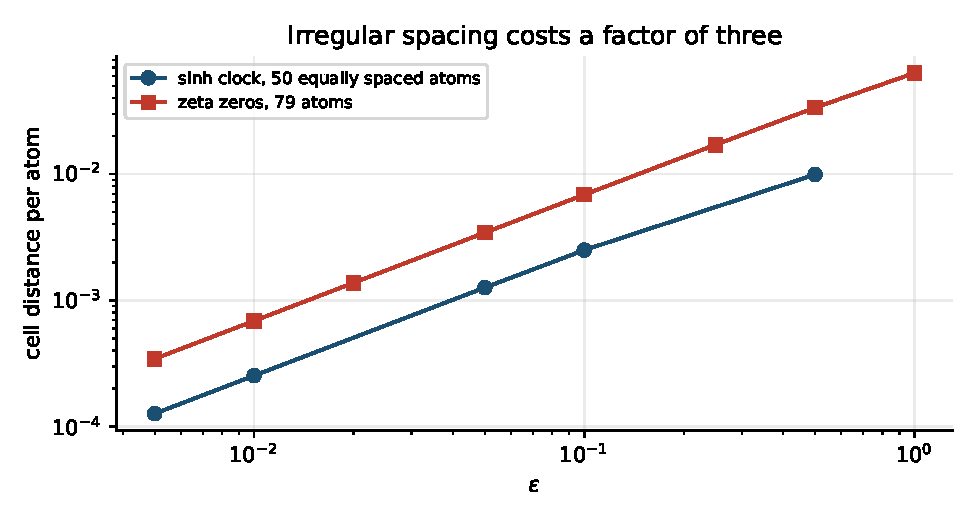
\includegraphics[width=0.72\textwidth]{fig/bench.pdf}
\caption{Cell distance divided by the number of atoms in the window, for the sinh clock ($50$ atoms, cells $(k-\frac12,k+\frac12]$) and for the $79$ zeros below height $200$ (Voronoi cells of Section~\ref{ch:distances}). Both vanish linearly in $\varepsilon$. For the sinh clock the undivided distance stays below $4\varepsilon/\pi$ whatever the number of atoms, so the gap between the curves depends on the window, and the factor of three in the title of the figure holds for these two windows only.}
\label{fig:ch3:bench}
\end{figure}

For the $79$ zeros below height $200$ the constant is $5.44$ (Section~\ref{ch:distances}), and it has a different origin. The zeros are irregularly spaced, so the mass that leaks out of a cell is no longer replaced by the mass that leaks in from its neighbours, and every cell contributes; Section~\ref{ch:spacing} reads the constant as a statistic of the spacings. Figure~\ref{fig:ch3:bench} divides both distances by the number of atoms, which gives $1.267\,\varepsilon/50=0.0253\,\varepsilon$ for the sinh clock and $5.44\,\varepsilon/79=0.069\,\varepsilon$ for the zeros. Their ratio, nearly three, depends on the window, since for the lattice the distance per atom falls like $1/N$ as the window grows to $N$ atoms. Williams' Thorin measure $2\sum_k\delta_{\pi^2k^2}$ of Table~\ref{tab:ch3:cat} needs no separate benchmark: it is the same lattice rescaled by $\pi$, with atoms of mass two, so its Thorin density at resolution $\varepsilon$ is $\frac2\pi\rho^{(0)}_{\varepsilon/\pi}(\theta/\pi)$ and its distances follow by scaling from the closed forms for the sinh clock.


\section{Exercises}\label{chap:foundations:ex}

\paragraph{On Section~\ref{ch:clock}.}
\begin{exercises}
\item Show from the Hadamard product \eqref{eq:ch2:hadamard} that $\sum_ka_k^{-1}=\xi''(\frac12)/(2\xi(\frac12))$, and compute it to ten digits from the P\'olya density by differentiating \eqref{eq:ch2:mgf} twice under the integral.
\item\label{ex:ch2:even} Prove that $\Phi$ is even by applying the theta transformation $1+2\omega(1/x)=\sqrt x\,(1+2\omega(x))$ to $\omega(x)=\sum_{n\ge1}e^{-\pi n^2x}$ and differentiating twice.
\item Show that if $X$ has the P\'olya density then $\E X^2=2\sum_ka_k^{-1}$, and deduce that the P\'olya law has variance $0.0462$.
\item Verify the first row of Table~\ref{tab:ch2:W} by summing $e^{-\gamma^2t}$ over the first forty zeros, and estimate the error of truncation using $N(T)\approx\frac T{2\pi}\log\frac T{2\pi e}$.
\item Show that an off line quadruple $\frac12\pm\delta\pm i\gamma$ contributes $2e^{-(\gamma^2-\delta^2)t}\cos(2\delta\gamma t)$ to $W(t)$, and find the first time at which that contribution is negative.
\item Show that at a basepoint $\alpha>1$ the Thorin density $v_\alpha(\sqrt z)/(2\pi\sqrt z)$ is bounded below by a positive multiple of $z^{-1/2}\log(2+z)$ for large $z$. Use Proposition~\ref{prop:struct} with the Riemann von Mangoldt formula, or, more simply, $v_\alpha(r)=\re[\frac1s+\frac1{s-1}-\frac12\log\pi+\frac12\psi(\frac s2)+\frac{\zeta'}\zeta(s)]$ at $s=\alpha+ir$ with Stirling's formula.
\item\label{ex:ch2:line} Let $\delta=0.49$, $\gamma_0=10.5$ and
\[
F(s)=\frac{\sinh(\pi(s-\frac12))}{\pi(s-\frac12)}\Big(1-\frac{(s-\frac12)^2}{(\delta+i\gamma_0)^2}\Big)\Big(1-\frac{(s-\frac12)^2}{(\delta-i\gamma_0)^2}\Big).
\]
Show that $F$ is entire of order one, positive on the real axis and symmetric under $s\mapsto1-s$, with zeros $\frac12\pm ik$ ($k\ge1$) and $\frac12\pm\delta\pm i\gamma_0$. Show that $\re(F'/F)(0.6+ir)>0$ for every real $r$, although $F$ vanishes at $0.99+10.5i$. (Put $\varepsilon=0.1$. The zeros $\frac12\pm\delta+i\gamma_0$ together contribute $2\varepsilon(t^2-\delta^2+\varepsilon^2)/((t^2+(\delta-\varepsilon)^2)(t^2+(\delta+\varepsilon)^2))$ at $t=r-\gamma_0$, and their conjugates the same expression at $t=r+\gamma_0$; it is at least $-2\varepsilon/(\delta^2-\varepsilon^2)$ and is nonnegative for $t^2\ge\delta^2-\varepsilon^2$; the zeros on the line contribute $\pi\re\coth(\pi(\varepsilon+ir))-\varepsilon/(\varepsilon^2+r^2)>0$, and $\pi\re\coth(\pi(\varepsilon+ir))\ge\pi\tanh(\pi\varepsilon)$.)
\end{exercises}

\paragraph{On Section~\ref{ch:ggc}.}
\begin{exercises}
\item Show that the $\mathrm{Gamma}(a,b)$ law, with shape $a$ and rate $b$, has Thorin measure $a\delta_b$, and that the sum of independent $\mathrm{Gamma}(a_j,b_j)$ variables has Thorin measure $\sum_ja_j\delta_{b_j}$.
\item Derive the Thorin measure of $\sech\sqrt u$ from the product $\cosh x=\prod_{k\ge1}(1+4x^2/((2k-1)^2\pi^2))$.
\item Prove that $\int_0^\infty\log(1+u/z)\,(2\pi\sqrt z)^{-1}dz=\sqrt u$ (integrate by parts), and deduce the entry for the positive stable law of index $\frac12$ in Table~\ref{tab:ch3:cat}.
\item Show that $e^{-t}(1+\frac1{2t})$ is completely monotone while $k(t)=e^{-t}(t+\frac12)$ is not monotone, and conclude that the infinitely divisible law with L\'evy density $e^{-t}(1+\frac1{2t})$ and no drift is in BO but not in SD.
\item For the sinh clock, derive $\mu^{(0)}_\varepsilon((0,\Theta^2])=m+\pi^{-1}\arctan(\varepsilon/\Theta)$ at $\Theta=m+\frac12$ from the periodicity of $\sum_{k\in\mathbb Z}P_\varepsilon(\theta-k)$, and check the first order value $0.00630\,\varepsilon$ of the mass defect at $\Theta=50.5$.
\item Show that the HCM property of $\varphi(u)=a/(a+u)$ reduces to complete monotonicity of $a^2/(a^2+auw+u^2)$ in $w$, and deduce that finite products of such functions are HCM.
\item\label{ex:ch3:cont} Show that the right side of \eqref{eq:ch3:ggc} extends to a holomorphic nonvanishing function on $\cut$. Deduce that if an entire function $F$ with $F(0)=1$ satisfies $1/F(u)=\E e^{-uH}$ for $0<u<1$, with $H$ a GGC, then $F$ has no zeros in $\cut$.
\end{exercises}

\chapter{Evaluating the Xi function}\label{chap:evaluation}


\section{The P\'olya route}\label{ch:polya}

P\'olya's integral \eqref{eq:ch2:mgf} evaluates $\xi$ in the complex plane from the kernel alone, without primes or zeros. In this chapter, $\delta$ always denotes the distance from the line of integration to the edge of the strip of analyticity of $\Phi$, not the displacement of an off line zero.

\subsection{The trapezoid rule on P\'olya's integral}\label{sec:ch4:trapezoid}

Recall the P\'olya kernel \eqref{eq:ch2:Phi} in Titchmarsh's normalisation \cite[Section 10.1]{Titchmarsh},
\begin{equation}\label{eq:Phi}
\Phi(u)=2\sum_{n\ge1}\big(2\pi^2n^4e^{9u/2}-3\pi n^2e^{5u/2}\big)\exp(-\pi n^2e^{2u}),
\end{equation}
even and positive on the real line, analytic in the strip $|\im u|<\pi/4$ (Section~\ref{ch:clock}) and doubly exponentially decaying in every closed substrip (proof of Proposition~\ref{prop:tilt}). With the P\'olya variable $X$ of density $p=\Phi/\Xi(0)$, the moment generating function \eqref{eq:ch2:mgf} and its derivative under the integral sign give, for every complex $s$,
\begin{equation}\label{eq:xi}
\frac{\xi(\tfrac12+s)}{\xi(\tfrac12)}=\E\,e^{sX}=\E\cosh(sX),\qquad \frac{\xi'(\tfrac12+s)}{\xi(\tfrac12)}=\E\,Xe^{sX},\qquad X\sim p,
\end{equation}
so the Thorin density \eqref{eq:rho} is $\pi^{-1}\re\{\E Xe^{sX}/\E e^{sX}\}$ at $s=\varepsilon+i\theta$. Throughout, $\log$ is the natural logarithm.

Analyticity and decay in the strip make the trapezoid rule with nodes $u_j=jh$ converge geometrically in $1/h$ \cite[Theorem 5.1]{TW14} (Exercise~\ref{ex:ch4:trapezoid}): for $s=\varepsilon+i\theta$,
\[
\Big|\int_{\R}\Phi(u)e^{su}\,du-h\sum_{j\in\mathbb Z}\Phi(jh)e^{sjh}\Big|\le \frac{2K_\eta(\varepsilon)\,e^{\eta|\theta|}}{e^{2\pi\eta/h}-1},\qquad 0<\eta<\pi/4,
\]
where $K_\eta(\varepsilon)=\int_{\R}|\Phi(x\pm i\eta)|\,e^{\varepsilon|x|}\,dx$, the same for both signs because $\Phi$ is real on the real axis. We write $K_\eta=K_\eta(0)$. Since $|\xi(\tfrac12+\varepsilon+i\theta)|$ decays like $e^{-\pi\theta/4}$, the relative error is at most of order $\exp\{(\eta+\pi/4)\theta-2\pi\eta/h\}$. With $h=1/200$ the bound is best for $\eta$ close to $\pi/4$, and at $\theta=200$ it is about $10^{-289}$; halving $h$ changes the computed values by less than $10^{-64}$.

The limit in practice is the cancellation in \eqref{eq:xi}: the integrand is of order one and the integral of order $e^{-\pi\theta/4}$, so at $b$ bits the rounding error is of order $2^{-b}e^{\pi\theta/4}$ relative to $|\xi|$, a loss of $\pi\theta/(4\log10)=0.341\,\theta$ decimal digits. Discretisation, rounding and the truncation of the $u$ axis at $|u|\le L$ can be budgeted separately. To reach $D$ correct digits at height $\theta$ one needs
\[
b\ \ge\ \Big(D+\frac{\pi\theta}{4\log10}\Big)\log_2 10,\qquad h\ \le\ \frac{2\pi\eta}{(D+0.682\,\theta)\log10},
\]
where the condition on $h$ uses $\eta+\pi/4\le\pi/2$. The truncation needs $\pi e^{2L}\ge(D+0.341\,\theta)\log10+|\varepsilon|L$, up to lower order terms.

We take $h=1/200$ and $L=3$, beyond which $\Phi$ is below $10^{-500}$, and work at $420$ bits ($126$ decimal digits): at height $200$, where $|\xi|$ is about $10^{-63}$, the cancellation consumes about half of them and leaves about $60$. Truncating the sum at $|j|\le J=L/h$ and folding it with the evenness of $\Phi$ gives, with $E=e^{sh}$,
\[
\xi(\tfrac12+s)\approx P(E)+P(E^{-1}),\qquad \xi'(\tfrac12+s)\approx Q(E)-Q(E^{-1}),
\]
\[
P(x)=\tfrac h2\Phi_0+h\sum_{j=1}^{J}\Phi_jx^j,\quad Q(x)=h^2\sum_{j=1}^{J}j\Phi_jx^j,
\]
with $\Phi_j=\Phi(jh)$ and $J=600$. The node values, the only place where the theta series is summed, are computed once for a given step, truncation and precision and serve every resolution and every height; one evaluation of $\xi$ and $\xi'$ then costs four polynomial evaluations in ball arithmetic \cite{Arb}, about $0.7$ ms at $420$ bits. The ball radii certify the rounding error only, and they overestimate it: at height $200$ they certify about $38$ digits of $\xi$ and, at $\varepsilon=0.005$, about $36$ of $\re(\xi'/\xi)$, while comparison with \texttt{mpmath} at $90$ digits shows that the values themselves carry about $63$.

\subsection{Zeros and Thorin masses below height 200}\label{sec:ch4:height200}

With the parameters of Section~\ref{sec:ch4:trapezoid}, the zeros and the Thorin masses below height $\Theta=200$ are computed at the eight resolutions $\varepsilon=1,\allowbreak0.5,\allowbreak0.25,\allowbreak0.1,\allowbreak0.05,\allowbreak0.02,\allowbreak0.01,\allowbreak0.005$ in five steps.
\begin{enumerate}
\item Compute $\Phi_j$, $0\le j\le J$, from \eqref{eq:Phi} at $420$ bits.
\item For each resolution $\varepsilon$, evaluate $\rho_\varepsilon(\theta_k)$ and $M_\varepsilon(\theta_k)=\pi^{-1}\arg\xi(\tfrac12+\varepsilon+i\theta_k)$, with the branch of the argument that vanishes at $\theta=0$, on the grid $\theta_k=k\varepsilon/8$ ($k\varepsilon/4$ at $\varepsilon=0.005$), $0\le\theta_k\le\Theta$. Since $\partial_\theta\arg\xi(\alpha+i\theta)=v_\alpha(\theta)$ with $\alpha=\tfrac12+\varepsilon$, $M_\varepsilon(\theta)=\mu_\varepsilon((0,\theta^2])$ is exactly the cumulative Thorin mass.
\item Locate the line zeros as sign changes of $\Xi(\theta)=\xi(\tfrac12+i\theta)$ on a grid of step $0.05$, reading each sign from a ball that excludes zero, and refine them by Newton's method using $\Xi'(\theta)=-\im\xi'(\tfrac12+i\theta)$.
\item Count all zeros with $0<\im\rho\le\Theta$ by the argument principle, $N(\Theta)=\pi^{-1}\Delta\arg\xi(s)$ along $2\to2+i\Theta\to\tfrac12+i\Theta$ \cite[Section 9.3]{Titchmarsh}.
\item Compare with $U_{\RH}$ in the metrics of Section~\ref{ch:distances}.
\end{enumerate}
Steps 3 and 4, which use the same two polynomials, together bound the number of off line zeros. Each sign change of $\Xi$ on the grid encloses at least one zero on the line, so $N(\Theta)$ minus the number of sign changes is an upper bound for the number of off line zeros with $0<\im\rho\le\Theta$. When the two numbers agree, every zero below height $\Theta$ is on the line and simple.

In step 2 the argument is accumulated from the increments $\arg(\xi(s_{k+1})/\xi(s_k))$ along $\re s=\frac12+\varepsilon$. The principal value is the true increment only if $\arg\xi$ changes by less than $\pi$ between consecutive points, which the samples cannot show; the grids are chosen so that every observed increment is below $\pi/2$ in modulus, a margin checked after the fact rather than a guarantee, and the largest observed was $0.29$. At large height $\xi$ underflows double precision ($|\xi|$ is about $10^{-335}$ at height $1000$), so the quotient must be formed in ball arithmetic before the argument is taken.

With $\Theta=200$ there are $79$ sign changes, and at none of the $4001$ grid points does the ball for $\Xi$ contain zero. The argument principle gives $N(200)=79.0000000000004$, with a largest increment of $0.02$ radians along the contour, and $\Theta=200$ lies between $\gamma_{79}=198.0153$ and $\gamma_{80}=201.2648$, so it is not an ordinate. The Newton refined roots agree to $5.0\times10^{-48}$ with the ordinates computed independently by \texttt{mpmath} \cite{mpmath} at $50$ digits. The computation thus recovers, with no input but \eqref{eq:Phi}, the classical fact that the $79$ zeros below height $200$ lie on the line and are simple \cite{Backlund,PT21}. It is not yet a proof: the argument increments are summed in double precision from samples, and the analytic error bounds are not added to the radii (Section~\ref{st:sec:wp2} lists what a certified version requires). Figure~\ref{fig:density} shows the computed density.

\begin{figure}[t]
\centering
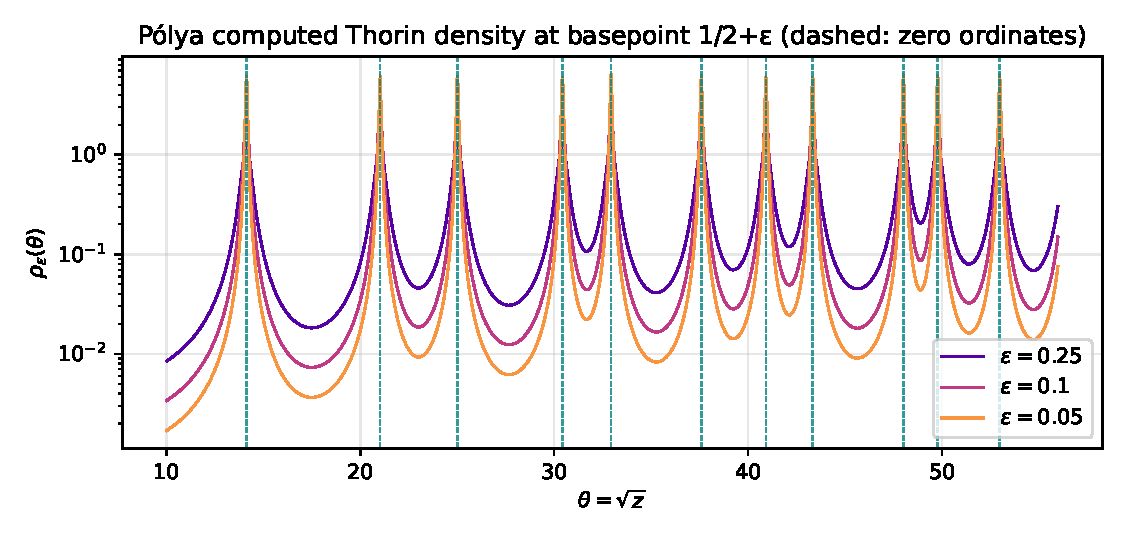
\includegraphics[width=0.95\textwidth]{fig/density.pdf}
\caption{The Thorin density $\rho_\varepsilon(\theta)$ at basepoint $\tfrac12+\varepsilon$ computed from the P\'olya density, for $\varepsilon=0.25,0.1,0.05$ and $10<\theta<56$, on a logarithmic scale; dashed lines mark the ordinates. Each ordinate carries a Cauchy kernel of height $1/(\pi\varepsilon)$ and mass one (Proposition~\ref{prop:struct}).}
\label{fig:density}
\end{figure}

\subsection{Tilting the contour into the strip}\label{sec:newcomp}

Since $\Phi$ is analytic in $|\im u|<\pi/4$, the integrals behind \eqref{eq:xi} can be taken along any horizontal line inside the strip.

\begin{proposition}\label{prop:tilt}
Let $0<\delta<\pi/4$ and $\eta=\pi/4-\delta$. For every complex $s$,
\begin{align*}
\xi\Big(\frac12+s\Big)&=e^{i\eta s}\int_{\R}\Phi(x+i\eta)\,e^{sx}\,dx,\\
\xi'\Big(\frac12+s\Big)&=e^{i\eta s}\int_{\R}(x+i\eta)\,\Phi(x+i\eta)\,e^{sx}\,dx .
\end{align*}
For real $x$, $|\Phi(x+i\eta)|\le C_\delta$ and $|(x+i\eta)\Phi(x+i\eta)|\le C_\delta$, with $C_\delta=O(\delta^{-5/2})$ as $\delta\to0$.
\end{proposition}

\begin{proof}
By Section~\ref{ch:clock}, $\Phi$ is analytic in $|\im u|<\pi/4$, and by the identity theorem its evenness $\Phi(u)=\Phi(-u)$ extends from the real line to the strip. For $u=x+iy$ with $|y|\le\eta$ and $x\ge0$ we have $\re e^{2u}=e^{2x}\cos2y\ge e^{2x}\sin2\delta$, so
\begin{equation}\label{eq:ch4:majorant}
|\Phi(x+iy)|\le2\sum_{n\ge1}\big(2\pi^2n^4e^{9x/2}+3\pi n^2e^{5x/2}\big)\exp(-\pi n^2e^{2x}\sin2\delta),
\end{equation}
and $\Phi$ decays doubly exponentially as $x\to+\infty$, uniformly in the closed strip $|y|\le\eta$; by evenness it does so as $x\to-\infty$ as well. Cauchy's theorem therefore moves the line of integration in $\xi(\tfrac12+s)=\int_{\R}\Phi(u)e^{su}\,du$, which is \eqref{eq:xi}, from $\im u=0$ to $\im u=\eta$, and the second identity follows in the same way from $\xi'(\tfrac12+s)=\int_{\R}u\Phi(u)e^{su}\,du$. Finally, $\sum_{n\ge1}n^ke^{-bn^2}=O(b^{-(k+1)/2})$ uniformly in $b>0$, so the majorant \eqref{eq:ch4:majorant} is $O(e^{-x/2}\delta^{-5/2})$ for $x\ge0$, of order $\delta^{-5/2}$ at $x=0$; with evenness this gives both bounds.
\end{proof}

On the real axis the integrand $\Phi(u)e^{su}$, with $s=\varepsilon+i\theta$, oscillates with frequency $\theta$, and its integral, of order $\theta^{7/4+\varepsilon/2}e^{-\pi\theta/4}|\zeta(\tfrac12+\varepsilon+i\theta)|$ by Stirling's formula, is exponentially smaller than the integrand. On the line $\im u=\eta$ the factor $e^{i\theta u}$ has constant modulus $e^{-\theta\eta}$ and leaves the integral as the prefactor $e^{i\eta s}$, which carries almost all of the decay of $\xi$; the integral that remains is of order $e^{-\delta\theta}$ up to the same factors, against an integrand of size at most $C_\delta e^{\varepsilon x}$. The cancellation thus drops from $e^{-\pi\theta/4}$ to $e^{-\delta\theta}$. The price is a larger kernel, by the factor $K_\eta/K_0$ with $K_0=\xi(\tfrac12)=0.497$, and a finer step, because the natural boundary at $\im u=\pi/4$ \cite[Chapter 11, Section 1.4, and Chapter 5, Section 3.2]{Remmert98} is now only $\delta$ away.

On the tilted line the kernel constant measures the size of the integrand and costs $\log_{10}K_\eta$ digits of precision. By Table~\ref{tab:ch4:Meta} it grows like $\delta^{-5/2}$, but $\log_{10}K_\eta$ stays under five even at $\delta=0.01$, which is negligible against the saving $(\pi/4-\delta)\theta/\log10$ at any height where tilting is worthwhile.

\begin{table}[htbp]
\centering\small
\begin{tabular}{rrr}
\toprule
$\delta=\pi/4-\eta$ & $K_\eta$ & $\max_x|\Phi(x+i\eta)|$\\
\midrule
0.6854 & 0.554 & 0.981\\
0.3927 & 2.52 & 3.24\\
0.2 & 19.0 & 15.4\\
0.1 & 126 & 76.5\\
0.05 & 774 & 415\\
0.02 & 7836 & 3938\\
0.01 & 43503 & 22207\\
\bottomrule
\end{tabular}
\caption{Size of the P\'olya kernel on lines inside its strip of analyticity, computed on a grid of step $0.002$ over $|x|\le6$; the first two rows are the lines $\eta=0.1$ and $\eta=\pi/8$. The growth is close to $\delta^{-5/2}$, as the majorant in the proof of Proposition~\ref{prop:tilt} predicts.}
\label{tab:ch4:Meta}
\end{table}

The trapezoid rule on the tilted line converges geometrically under two conditions (Exercise~\ref{ex:ch4:alias}). By Poisson summation its error is $\sum_{k\ne0}I(\theta+2\pi k/h)$, where $I(t)=\int_{\R}\Phi(x+i\eta)e^{\varepsilon x}e^{itx}\,dx=e^{\eta t-i\eta\varepsilon}\xi(\tfrac12+\varepsilon+it)$. The integrand is analytic in a strip that extends $\delta$ above the line and $\pi/2-\delta$ below it, and correspondingly $|I(t)|$ is of order $e^{-\delta t}$ as $t\to+\infty$ and $e^{-(\pi/2-\delta)|t|}$ as $t\to-\infty$, up to the factors of Stirling's formula. Relative to $I(\theta)$ the terms with $k\ge1$ are of order $e^{-2\pi\delta k/h}$, and those with $k\le-1$ are small only when the step resolves the oscillation $e^{i\theta x}$ with a margin. For $D$ correct digits this gives
\begin{equation}\label{eq:ch4:tiltcond}
\frac1h\ \ge\ \frac{D\log10}{2\pi\delta},\qquad \frac{2\pi}h\ \ge\ \theta+\frac{\delta\theta+D\log10}{\pi/2-\delta},
\end{equation}
up to terms of order $\log\theta+\log(1/h)$. The first condition asks for about $D\log10/(2\pi\delta)$ nodes per unit length, $458$ at $D=25$ and $\delta=0.02$, that is $h\le2.2\times10^{-3}$. The second is the binding one at large height: at $\delta=0.02$ and $25$ digits it is the stronger from about $\theta=2800$ on, and it asks for $h\le1.23\times10^{-3}$ at $\theta=5000$ and $h\le8.8\times10^{-4}$ at $\theta=7005$.

Taking $\delta$ proportional to $1/\theta$ holds the loss $\delta\theta/\log10$ fixed, so the working precision grows only through the $\log_{10}K_\eta$ digits of the kernel constant, about $\frac52\log_{10}(1/\delta)$, while both conditions \eqref{eq:ch4:tiltcond} make the number of nodes, and with it the cost per point, grow linearly in $\theta$ up to a logarithmic factor from the truncation.

\subsection{Precision and cost of the tilted route}\label{sec:ch4:budget}

The tilt makes height $5000$ accessible (Table~\ref{tab:tilt}).

\begin{table}[t]
\centering\small
\begin{tabular}{rrrrrrl}
\toprule
$\delta$ & bits & nodes & $\theta$ & error of $\xi'/\xi$ & ms per point & untilted digits needed\\
\midrule
0.10 & 200 & 2001 & 200 & $<2\times10^{-45}$ & 7 & 68\\
0.10 & 200 & 2001 & 500 & $9.8\times10^{-42}$ & 7 & 171\\
0.10 & 200 & 2001 & 1000 & $1.8\times10^{-20}$ & 7 & 341\\
0.02 & 220 & 8401 & 1000 & $<6\times10^{-45}$ & 28 & 341\\
0.02 & 220 & 8401 & 2000 & $<4\times10^{-45}$ & 28 & 682\\
0.02 & 220 & 8401 & 5000 & $2.9\times10^{-25}$ & 28 & 1705\\
\bottomrule
\end{tabular}
\caption{The tilted P\'olya route at $\varepsilon=0.05$, compared with \texttt{mpmath} at $50$ digits. Errors are absolute errors of $\xi'/\xi$, which bound those of its real part, and $<$ marks the entries at the floor set by rounding the tilted value to $45$ significant digits. The rows with $2001$ nodes use the step $h=0.004$ and the truncation $L=4$, those with $8401$ nodes $h=0.001$ and $L=4.2$. The last column is the number of digits, $0.341\,\theta$, that the untilted route loses to cancellation at the same height.}
\label{tab:tilt}
\end{table}

On the tilted line the rounding term of Section~\ref{sec:ch4:trapezoid} becomes $2^{-b}e^{\delta\theta}$ times the kernel constant, and the step obeys \eqref{eq:ch4:tiltcond}. Table~\ref{tab:ch4:budget} compares the working precision of the two routes. The formula of the table for the tilted bits is conservative: it ignores the factor $\theta^{7/4+\varepsilon/2}$ in $|\xi(\tfrac12+\varepsilon+i\theta)|$, worth about six digits at $\theta=5000$, and it adds five digits for the kernel constant. The run at $\theta=5000$ in Table~\ref{tab:tilt} used $220$ bits, fewer than the $244$ of Table~\ref{tab:ch4:budget}, and returned $25$ digits; the Lehmer pair of Section~\ref{sec:ch5:lehmer} was computed with $256$ bits at $\delta=0.01$, where the formula asks for $201$.

\begin{table}[htbp]
\centering\small
\begin{tabular}{rrrrr}
\toprule
height $\theta$ & target digits & bits (untilted) & bits (tilted, $\delta=0.02$) & nodes (tilted)\\
\midrule
100 & 30 & 213 & 119 & 8400\\
200 & 30 & 326 & 122 & 8400\\
1000 & 30 & 1233 & 145 & 8400\\
5000 & 25 & 5748 & 244 & 8400\\
7005 & 25 & 8020 & 302 & 8400\\
\bottomrule
\end{tabular}
\caption{Working precision needed by the untilted and the tilted P\'olya route for $D$ target digits. The untilted bits are $(D+\pi\theta/(4\log10))\log_210$ and the tilted bits $(D+\delta\theta/\log10+5)\log_210$, where the $5$ digits cover $\log_{10}K_\eta<5$ for $\delta\ge0.01$. At $\theta=7005$ the second condition in \eqref{eq:ch4:tiltcond} asks for $h\le8.8\times10^{-4}$, so $8400$ nodes give $25$ digits there only with a truncation near $|x|\le3.7$, the smallest that suffices.}
\label{tab:ch4:budget}
\end{table}

Because the tilt reduces the cancellation to $e^{-\delta\theta}$, ordinary double precision suffices at moderate height. With $\delta=0.15$ and the node values rounded to double, a vectorised evaluation agrees with the ball arithmetic values of $\rho_{0.05}$ to within an absolute error of $2.8\times10^{-12}$ for $\theta\le50$, $1.3\times10^{-9}$ for $\theta\le100$ and $7.6\times10^{-7}$ for $\theta\le150$, at $93\,\mu$s per point. The untilted route fails in double precision above $\theta\approx40$ (Exercise~\ref{ex:ch4:double}).



\subsection{Ball arithmetic on the tilted line}\label{sec:ch4:balls}

Horner's rule, which serves the untilted evaluator well, fails in ball arithmetic on the tilted line. The tilted evaluator writes the trapezoid sum as one polynomial of degree $2J$ in $E=e^{sh}$, with coefficients $h\Phi(x_k+i\eta)$ for $x_k$ running from $-L$ to $L$, times the prefactor $e^{i\eta s}E^{-J}$. With $2001$ nodes, $\delta=0.1$ and $200$ bits, the radius of the Horner recursion grew by a factor of about $1.3$ per step, and the final ball at $\theta=100$ had radius $10^{109}$ although its midpoint was correct to many digits. Evaluating each exponential $e^{sx_k}$ directly and summing gives balls of radius about $10^{-55}$ at the same point.

The cause is the wrapping effect of rectangular complex balls. Arb stores a complex number as a real ball and an imaginary ball \cite{Arb}, so a multiplication by $E=e^{\varepsilon h}e^{i\theta h}$ rotates the midpoint but multiplies the radii by $e^{\varepsilon h}(|\cos\theta h|+|\sin\theta h|)$, up to rounding; at $\theta h=0.4$ this factor is $1.31$. In Horner's rule the coefficient of $E^k$ passes through $k$ such multiplications. On the untilted line the effect is contained. The polynomials are folded at $x=0$, so the coefficient at $x=jh$ passes through at most $600$ multiplications, and the coefficients $h\Phi(jh)$ decay like $\exp(-\pi e^{2jh})$, so those that pass through many multiplications are negligible and the radii stay far below $|\xi|$ up to height $200$. On the tilted line the coefficients decay only like $\exp(-\pi e^{2x}\sin2\delta)$, and the coefficient at $x$ passes through $(x+L)/h$ multiplications. With $h=0.004$ and $L=4$, which give $2001$ nodes, the coefficients near $x=2$ are still of order $10^{-12}$ at $\delta=0.1$, and they pass through about $1500$ multiplications, which enlarge their radii by a factor of about $10^{176}$.

\section{Classical evaluators, Turing's method and the P\'olya route}\label{ch:classical}

The classical evaluators on the critical line pay for height differently and, at large height, far less than the P\'olya route, tilted or not.

\subsection{The Riemann Siegel formula, Gram points and certified counts}\label{sec:ch5:turing}

On the critical line $\zeta(\frac12+it)=e^{-i\vartheta(t)}Z(t)$, where $\vartheta(t)=\im\log\Gamma(\frac14+\frac{it}2)-\frac t2\log\pi$ is the Riemann Siegel theta function and $Z(t)$ is real for real $t$. Write $m=\lfloor\sqrt{t/2\pi}\rfloor$ and $q=\sqrt{t/2\pi}-m$. For every $K\ge0$,
\[
Z(t)=2\sum_{n\le m}\frac{\cos(\vartheta(t)-t\log n)}{\sqrt n}+(-1)^{m-1}\Big(\frac t{2\pi}\Big)^{-1/4}\sum_{j=0}^{K}C_j(q)\Big(\frac t{2\pi}\Big)^{-j/2}+R_K(t),
\]
where $R_K(t)=O(t^{-(2K+3)/4})$ as $t\to\infty$, $C_0(q)=\cos(2\pi(q^2-q-\frac1{16}))/\cos(2\pi q)$, and the higher $C_j$ are given in \cite[Section 7.5]{Edwards} and \cite{Gabcke79}. This asymptotic expansion was found in Riemann's unpublished notes and published by Siegel \cite{Siegel32}.

The main sum is the approximate functional equation $\zeta(s)=\sum_{n\le x}n^{-s}+\chi(s)\sum_{n\le y}n^{s-1}+\cdots$, where $\zeta(s)=\chi(s)\zeta(1-s)$ and $2\pi xy=t$ \cite[Chapter 4]{Titchmarsh}, taken at $x=y=\sqrt{t/2\pi}$ and written for $Z$; the $C_j$ correct for the abrupt truncation at $n=m$. The terms are bounded by $2$ and there is no exponential cancellation, so double precision suffices at every height computed in this book; near height $10^{12}$ and above, the phases $\vartheta(t)-t\log n$ must be reduced modulo $2\pi$ in higher precision. Gabcke's thesis gives explicit bounds for the remainders $R_K$ with $K\le10$ \cite{Gabcke79}, and with them the formula can be used in rigorous computation.

To evaluate $Z$ at many points near height $T$, Odlyzko and Sch\"onhage \cite{OS88} compute the main sum on a grid by fast Fourier transforms and rational function evaluation, and interpolate between grid points by band limited interpolation. About $T^{1/2}$ values then cost $T^{1/2+o(1)}$ operations, that is $T^{o(1)}$ per point. Odlyzko compared the spacings of the zeros near zero number $10^{12}$ with the Gaussian unitary ensemble \cite{Odlyzko87}, and with the algorithm he later took such computations to zero numbers $10^{20}$ \cite{Odlyzko92} and $10^{22}$ \cite{Odlyzko01}.

The classical searches for zeros on the line sample $Z$ at the Gram points $g_n$, defined by $\vartheta(g_n)=n\pi$ \cite[pp.~301 and 302]{Gram03}. There $Z(g_n)$ usually has the sign of $(-1)^n$, and each Gram interval $[g_{n-1},g_n)$ usually contains exactly one zero. This is Gram's law, and it fails with positive frequency \cite[Corollary 5.4]{Trudgian11b}. Call $g_n$ good when $(-1)^nZ(g_n)>0$, and call an interval $[g_j,g_{j+k})$ between consecutive good Gram points a Gram block. Rosser's rule asserts that such a block contains exactly $k$ zeros \cite{RYS69}, \cite[Section 7.3]{Trudgian11b}. It holds far longer than Gram's law, since its first exception is the block that begins at $g_{13\,999\,525}$ \cite[Table 3]{Brent79}, but it too fails with positive frequency \cite[Corollary 7.8]{Trudgian11b}. Counting sign changes of $Z$ gives a lower bound for the number of zeros on the line. The difficulty is to show that none is missing, whether off the line or in a close pair that produces no sign change.

Turing's answer \cite{Turing53} uses the counting function $N(T)=\vartheta(T)/\pi+1+S(T)$, where, for $T$ not an ordinate, $\pi S(T)=\arg\zeta(\frac12+iT)$, the argument being defined by continuous variation along $2\to2+iT\to\frac12+iT$. The function $S$ is small on average: Littlewood proved $\int_0^TS(t)\,dt=O(\log T)$ \cite[Theorem 9.9(A)]{Titchmarsh}, and Turing gave explicit constants for $|\int_{t_1}^{t_2}S(t)\,dt|$, later sharpened by Trudgian \cite{Trudgian11}. If the sign changes found near height $T$ were fewer than $N(T)$, then $S$ would be displaced by at least $2$ over an interval long enough to violate the integral bound. The count is therefore certified by locating the sign changes in a range slightly beyond $T$ and checking them against Turing's bound for $\int S$. The method never evaluates $\zeta$ off the line. Turing's published argument contained errors, corrected by Lehman \cite{Lehman70}, and the corrected method underlies every large verification since, including Platt and Trudgian's to height $3\times10^{12}$ \cite{PT21}.

Before Turing, counts were certified by Backlund's method. Since $\re\zeta(2+it)\ge2-\zeta(2)>0$ for every $t$, it suffices to check that $\re\zeta(\sigma+iT)\ne0$ for $\frac12\le\sigma\le2$: then $\arg\zeta$ stays in $(-\frac\pi2,\frac\pi2)$ along the whole path, so $|S(T)|<\frac12$ and $N(T)$ is the integer nearest to $\vartheta(T)/\pi+1$. Backlund carried this out for $T=200$ \cite{Backlund} and Hutchinson for $T=300$ \cite[pp.~54 to 57]{Hutchinson25}, \cite{Trudgian11}.

\subsection{The P\'olya route beside the classical evaluators}

The P\'olya route evaluates $\xi$ and $\xi'$ on and off the line, at $\tfrac12+\varepsilon+i\theta$, from the P\'olya kernel, and so delivers the Thorin density $\rho_\varepsilon$, its mass and the zero count from one evaluator. Its count has the logic of Turing's certificate: when the sign changes of $\Xi$ and the argument principle count $N(T)$ agree, every zero up to height $T$ is on the line and simple (Section~\ref{sec:ch4:height200}).

The methods differ most in how their cost grows with height (Table~\ref{tab:compare}). The untilted P\'olya route needs about $0.341\,t$ extra digits; and by the budget of Section~\ref{sec:ch4:trapezoid} its step must be below $\pi/t$, so that its number of nodes grows linearly with $t$ as well. The cause is aliasing. By Poisson summation the trapezoid sum at $s=\varepsilon+it$ equals $\sum_{k\in\mathbb Z}\xi(\frac12+s-2\pi ik/h)$, and the term $k=1$, at height $t-2\pi/h$, is exponentially larger than $\xi(\frac12+s)$ once $t>\pi/h$. The tilted contour of Section~\ref{sec:newcomp} cuts the loss of digits to about $\delta t/\log10$, but aliasing still requires $2\pi/h>t$, by the second condition in \eqref{eq:ch4:tiltcond}, so there too the number of nodes grows linearly with $t$.

\begin{table}[t]
\centering\footnotesize
\begin{tabular}{p{0.144\linewidth}p{0.2\linewidth}p{0.2\linewidth}p{0.325\linewidth}}
\toprule
 & \raggedright Riemann Siegel and Turing & Odlyzko Sch\"onhage & P\'olya route\tabularnewline
\midrule
object & sign changes of $Z(t)$ & zeros in blocks, statistics & Thorin density $\rho_\varepsilon$, mass, count\\
where evaluated & critical line & critical line & line $\re s=\tfrac12+\varepsilon$ and contour\\
count certificate & Gram points and $\int S$ & Turing's method & argument principle count equal to the number of sign changes; computed, not yet certified\\
cost per point & $\sqrt{t/2\pi}$ terms, double & amortised, $t^{o(1)}$ & $0.341\,t$ extra digits and step below $\pi/t$ (untilted); $\delta t/\log10$ digits and step below $2\pi/t$ (tilted)\\
accuracy & asymptotic remainder & asymptotic remainder & spectral; rounding certified by balls\\
reach & $t\approx1540$ in 1953 & $t\approx10^{20}$ and beyond \cite{Odlyzko92,Odlyzko01} & $t\approx7005$ (Section~\ref{sec:ch5:lehmer}); $25$ digits at $t=5000$ (Table~\ref{tab:tilt})\\
\bottomrule
\end{tabular}
\caption{The Riemann Siegel formula with Turing's method, the Odlyzko Sch\"onhage algorithm and the P\'olya route: what each computes, where, with what certificate, at what cost per point, and how far it has reached.}
\label{tab:compare}
\end{table}

\label{sec:ch5:hybrid}The distances of Section~\ref{ch:distances} do not depend on how $\xi$ is evaluated, and this suggests a hybrid at large height. The approximate functional equation holds off the critical line \cite[Chapter 4]{Titchmarsh}, so Riemann Siegel type expansions of $\zeta$ \cite[Theorems 3.1 and 4.2]{AriasDeReyna11} and of $\zeta'$, and the Odlyzko Sch\"onhage algorithm for blocks of points, apply at $\tfrac12+\varepsilon+i\theta$ as well. With them as the evaluator and Odlyzko's zeros \cite{OdlyzkoTables} as the RH reference, one could compute $\rho_\varepsilon$, the matched total variation and the positivity margin at the heights of Odlyzko's computations, from about $10^{11}$ to beyond $10^{20}$, while the tilted P\'olya route supplies values with explicitly bounded errors on low windows.

\subsection{Two computations beyond the untilted route}

\subsubsection{A Lehmer pair near height 7005}\label{sec:ch5:lehmer}

Lehmer found two zeros that are unusually close, $\gamma_{6709}=7005.0629$ and $\gamma_{6710}=7005.1006$ \cite[pp.~297 and 298]{Lehmer56}, at distance $0.0377$, the classical example of a Lehmer pair; such pairs give lower bounds for the de Bruijn Newman constant \cite{CSV94} (Section~\ref{sec:ch21:bounds}). The untilted P\'olya route cannot reach this height: it would need about $2400$ digits and a step below $4.5\times10^{-4}$. The tilted route with $\delta=0.01$, $256$ bits, $13001$ nodes, step $6\times10^{-4}$ and truncation $|x|\le3.9$ computes $\Xi(\theta)e^{\pi\theta/4}$ at $34$ milliseconds per point. On a grid of step $0.005$ it finds sign changes in $(7005.060,7005.065)$ and $(7005.100,7005.105)$, the two members of the pair (Figure~\ref{fig:ch5:lehmer}).

The Thorin density shows what resolution separates them. A single zero on the line produces a Cauchy peak of height $1/(\pi\varepsilon)$, that is $6.4$, $15.9$ and $31.8$ at $\varepsilon=0.05$, $0.02$ and $0.01$. The largest values of $\rho_\varepsilon$ on the grid are $11.18$, $19.58$ and $33.89$. At $\varepsilon=0.05$ the two peaks have merged into one of nearly double height; at $\varepsilon=0.02$ they are partly separated; at $\varepsilon=0.01$ each carries its own peak, lifted slightly by its neighbour. The Cauchy kernel predicts this: two kernels with half width at half maximum $\varepsilon$ at distance $g$ have a single maximum when $g\le2\varepsilon/\sqrt3$ and two maxima when $g>2\varepsilon/\sqrt3$. With $g=0.0377$ the pair is resolved as two peaks for $\varepsilon<\sqrt3\,g/2\approx0.033$. The criterion concerns two isolated kernels; Exercise~\ref{ex:ch5:cauchy} proves it and asks how much the other zeros move the threshold.

\begin{figure}[htbp]
\centering
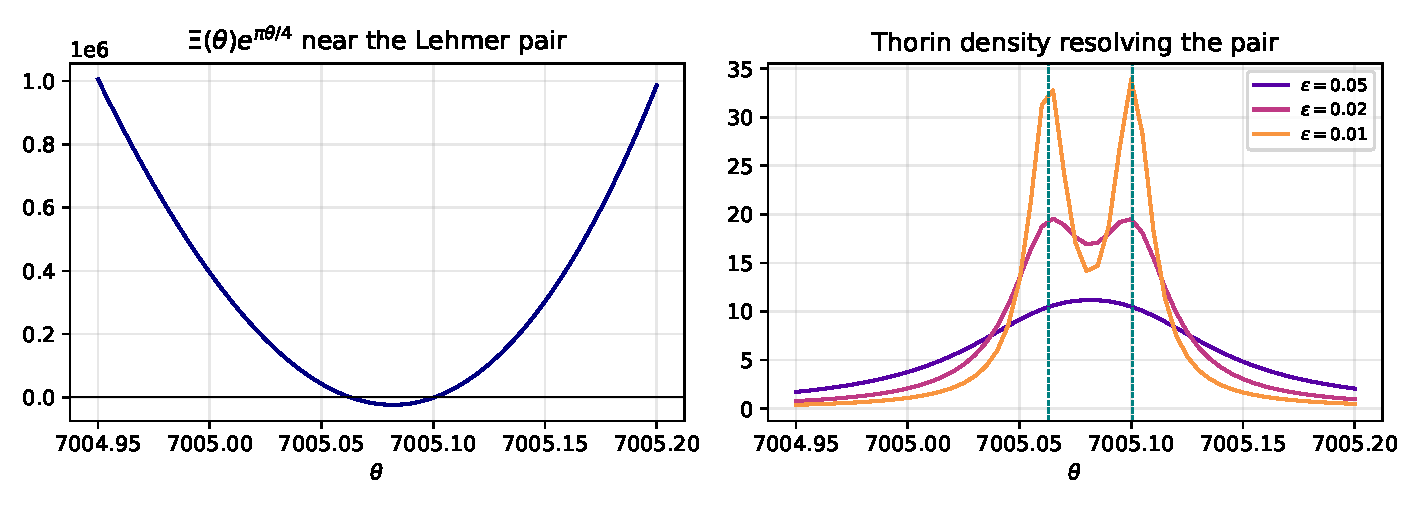
\includegraphics[width=\textwidth]{fig/lehmer.pdf}
\caption{The Lehmer pair near $7005$ computed by the tilted P\'olya route: $\Xi(\theta)e^{\pi\theta/4}$ (left) and the Thorin density at three resolutions (right), drawn through values on a grid of step $0.005$, with the two ordinates dashed.}
\label{fig:ch5:lehmer}
\end{figure}

\subsubsection{The zero count at height 1000}\label{sec:ch5:count}

Proposition~\ref{prop:zerodensity} of Section~\ref{ch:turing} gives the unconditional count $N(T)=M_{1/2}(T)+\tau_{1/2}(T)$, where $M_{1/2}(T)=\pi^{-1}\arg\xi(1+iT)$ is the cumulative Thorin mass at resolution $\frac12$, that is at the basepoint one of Section~\ref{ch:basepoint}, and $\tau_{1/2}(T)$ is $\pi^{-1}$ times the change of $\arg\xi$ along the segment from $1+iT$ to $\frac12+iT$. With the tilted route ($\delta=0.1$, $200$ bits, step $0.004$ and truncation $|x|\le4.2$, that is $2101$ nodes), $10000$ steps of $0.1$ along $\re s=1$ and $2000$ steps along the segment, we find
\[
M_{1/2}(1000)=648.7562315041018,\qquad \tau_{1/2}(1000)=0.2437684958980,
\]
\[
M_{1/2}(1000)+\tau_{1/2}(1000)=648.9999999999999,
\]
so $N(1000)=649$, with a largest argument increment of $0.43$ radians. The computation took $77.5$ seconds; \texttt{mpmath}'s \texttt{nzeros} returns $649$ in $0.017$ seconds. Where Backlund bounds the argument, this computation accumulates it from samples, and ball arithmetic certifies the rounding in each sampled value but not the absence of winding between samples. The count is therefore computed rather than certified. Certifying it would need, besides the analytic error bounds of Section~\ref{ch:polya}, an enclosure of $\xi$ between consecutive sample points $s_k$ and $s_{k+1}$, for instance a check that $\re\,\xi(s)/\xi(s_k)>0$ on a ball containing the segment between them.

For counting and locating zeros at height, the Riemann Siegel family with Turing's method is faster by orders of magnitude, and the P\'olya route is not a competitor there. It reads the count as an integer from a smooth quantity, the Thorin mass, with no Gram point bookkeeping; it gives the zero density strip by strip (Section~\ref{ch:turing}); and it evaluates objects that the classical methods, used on the critical line, do not compute: Thorin densities and their distances to $U_{\RH}$.

\section{A worked computation from first principles}\label{ch:worked}

Where Section~\ref{ch:classical} took the tilted route to large height, we return to the untilted route and follow one small computation with it at low height, from the theta series to a Thorin mass and a zero. Every value can be reproduced with \texttt{code/polya\_flint.py} (Section~\ref{app:code:eval}).

The parameters are those of Section~\ref{sec:ch4:trapezoid}, step $h=1/200$ and truncation $|u|\le3$, and the working precision is $240$ bits, about $72$ decimal digits, the default of the code. As there, $s$ is the displacement from $\frac12$: with $E=e^{sh}$ and $\Phi_j=\Phi(jh)$, the evaluator returns $\xi(\frac12+s)\approx P(E)+P(E^{-1})$ and $\xi'(\frac12+s)\approx Q(E)-Q(E^{-1})$, from which $\rho_\varepsilon(\theta)=\pi^{-1}\re(\xi'/\xi)(\frac12+\varepsilon+i\theta)$.

\paragraph{Step one: the kernel at a single point.} At $u=0$ the kernel \eqref{eq:ch2:Phi} is
\[
\Phi(0)=2\sum_{n\ge1}\big(2\pi^2n^4-3\pi n^2\big)e^{-\pi n^2}.
\]
The $n$th term is of order $n^4e^{-\pi n^2}$, and the terms with $n\ge8$ add up to less than $10^{-82}$, so seven terms already give more than eighty digits:
\[
\Phi(0)=0.89339380093424688817396933410941822644084873418965\ldots.
\]
The ball returned by the arithmetic has radius $3\times10^{-71}$.

\paragraph{Step two: the coefficients.} The truncation leaves $601$ nodes $u_j=jh$, $0\le j\le600$. The coefficients of $P$ are $\frac h2\Phi_0$ and $h\Phi_j$, $1\le j\le600$, and those of $Q$ are $h^2j\Phi_j$; the first is
\[
\tfrac h2\Phi(0)=0.00223348450233561722043492333527354556610\ldots.
\]
The coefficients decay doubly exponentially. By the asymptotic formula of Section~\ref{ch:clock}, $\Phi(2.7)\approx4\pi^2e^{12.15}\exp(-\pi e^{5.4})\approx6\times10^{-296}$, so the coefficients beyond $j\approx540$ are below $10^{-297}$.

\paragraph{Step three: $\xi(\frac12)$ as a trapezoid sum.} At $s=0$, $E=e^{sh}=1$, and $\xi(\frac12)=2P(1)$ is the trapezoid sum of the kernel:
\[
\xi(\tfrac12)=0.4971207781883141099127737396853977198072936095577\ldots,
\]
with ball radius $5\times10^{-71}$. \texttt{mpmath}'s evaluation from the definition, $\frac12z(z-1)\pi^{-z/2}\Gamma(z/2)\zeta(z)$ at $z=\frac12$ in thirty digit arithmetic, gives
\[
0.497120778188314109912773739685,
\]
agreeing to every digit. By the bound of Section~\ref{sec:ch4:trapezoid} the quadrature error is below $10^{-400}$, so the seventy digits are set by the working precision, not by the rule.

\paragraph{Step four: the Thorin density at the first ordinate.} At
\[
s=0.1+14.134725141734693790i,
\]
that is at resolution $\varepsilon=0.1$ and the first ordinate $\gamma_1$, the evaluator returns $\xi(\frac12+s)$ and $\xi'(\frac12+s)$, and
\[
\rho_{0.1}(\gamma_1)=\frac1\pi\re\frac{\xi'}{\xi}\Big(\frac12+s\Big)=3.18525309376337225967538\ldots.
\]
A single Cauchy kernel of width $0.1$ contributes exactly $1/(\pi\varepsilon)=3.18309886183791$ at its centre. By Proposition~\ref{prop:struct} the excess, $0.00215423$, is the sum of the contributions of every other zero, $\sum_{j\ne1}[P_{0.1}(\gamma_1-\gamma_j)+P_{0.1}(\gamma_1+\gamma_j)]$, plus the reflected kernel of $\gamma_1$ itself. The nearest neighbour, at distance $6.887$, contributes $6.7\times10^{-4}$, the reflected kernel $4\times10^{-5}$, and the many distant zeros, whose contributions decay like the inverse square of the distance, the remaining $1.4\times10^{-3}$. Figure~\ref{fig:ch5b:decomp} shows the same decomposition along the whole stretch between the first two zeros.

\begin{figure}[htbp]
\centering
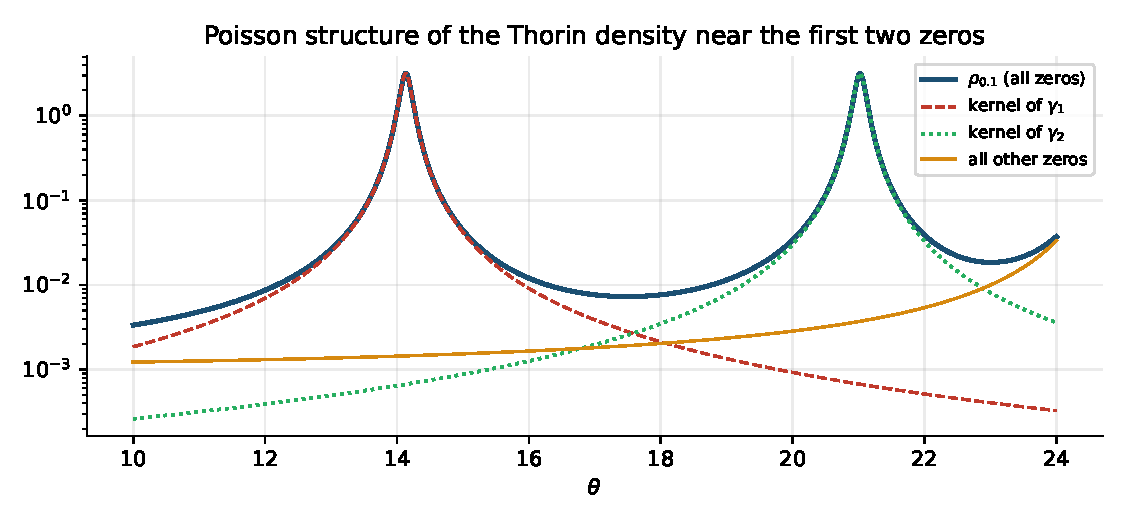
\includegraphics[width=0.85\textwidth]{fig/decomp.pdf}
\caption{The Thorin density $\rho_{0.1}$ near the first two zeros, split into the kernel of $\gamma_1$, the kernel of $\gamma_2$ and the rest, that is all other zeros and the reflected kernels at $-\gamma_j$, computed from the first $1700$ zeros without a tail correction.}
\label{fig:ch5b:decomp}
\end{figure}

Between zeros the density is small but strictly positive. At $\theta=17$, between $\gamma_1$ and $\gamma_2=21.022$,
\[
\rho_{0.1}(17)=0.0076857707896205949783\ldots,
\]
close to the minimum of $\rho_{0.1}$ between the two zeros (Figure~\ref{fig:ch5b:decomp}). Lagarias's criterion \cite{Lagarias} asks for this positivity at every $\theta$ and every resolution $\varepsilon>0$.

\paragraph{Step five: the Thorin mass up to height $20$.} The cumulative Thorin mass of Section~\ref{sec:ch4:height200} is $M_\varepsilon(\theta)=\mu_\varepsilon((0,\theta^2])=\pi^{-1}\arg\xi(\frac12+\varepsilon+i\theta)$, with the argument continued from the real axis. Stepping along the line $\frac12+0.1+i\theta$ from $\theta=0$ to $\theta=20$ in $1600$ steps of $\varepsilon/8=0.0125$, as in that section, and accumulating the arguments of the quotients $\xi(\frac12+s_{k+1})/\xi(\frac12+s_k)$, where $s_k=0.1+i\theta_k$ and $\theta_k=0.0125\,k$, gives
\[
\mu_{0.1}\big((0,400]\big)=M_{0.1}(20)=1.0509304\ldots,
\]
in $0.77$ seconds. There is exactly one zero below height $20$. By Proposition~\ref{prop:mass} the excess $0.0509$ over the count agrees to $O(\varepsilon^2)$ with the first order mass defect $-(\varepsilon/\pi)\Xi'(20)/\Xi(20)$ (Exercise~\ref{ex:ch5b:mass}): it is the mass carried across the edge $\theta=20$ by the Cauchy tails of the first zero and of the zeros above $20$, while what crosses $\theta=0$ is returned exactly by the reflected kernels. Adding $\tau_{0.1}(20)$, which is $\pi^{-1}$ times the change of $\arg\xi$ along the segment from $\frac12+0.1+20i$ to $\frac12+20i$, returns the integer $1$, as Proposition~\ref{prop:zerodensity} requires.

\paragraph{Step six: locating the first zero.} The ordinate $\gamma_1$ in step four was only a convenient point, and the density would have revealed it, up to the small shift caused by the other zeros, as the location of its first peak. To locate it from the P\'olya route alone, one evaluates $\Xi(\theta)=\xi(\frac12+i\theta)$ on a grid, finds the sign change in $(14.10,14.15)$, and refines by Newton's method with $\Xi'(\theta)=-\im\xi'(\frac12+i\theta)$; six iterations give $\gamma_1$ to forty digits. Section~\ref{sec:ch4:height200} refines all $79$ zeros below height $200$ in the same way, at $420$ bits.


\section{Exercises}\label{chap:evaluation:ex}

\paragraph{On Section~\ref{ch:polya}.}
\begin{exercises}
\item\label{ex:ch4:trapezoid} Let $f$ be analytic in a strip containing $|\im u|\le\eta$, with $\int_{\R}|f(x\pm i\eta)|\,dx\le M$ and $f(u)\to0$ uniformly as $|\re u|\to\infty$ in $|\im u|\le\eta$. Prove that $|\int_{\R}f(u)\,du-h\sum_jf(jh)|\le2M/(e^{2\pi\eta/h}-1)$ by writing the error as the sum of the integrals, from left to right, of $f(u)(e^{-2\pi iu/h}-1)^{-1}$ along $\im u=\eta$ and of $f(u)(e^{2\pi iu/h}-1)^{-1}$ along $\im u=-\eta$ \cite[Theorem 5.1]{TW14}. Deduce the bound of Section~\ref{sec:ch4:trapezoid}.
\item\label{ex:ch4:alias} Let $g(x)=\Phi(x+i\eta)e^{\varepsilon x}$ with $\eta=\pi/4-\delta$ and $\varepsilon\ge0$, and $I(t)=\int_{\R}g(x)e^{itx}\,dx$. Show by Poisson summation that $h\sum_{j\in\mathbb Z}g(jh)e^{i\theta jh}-I(\theta)=\sum_{k\ne0}I(\theta+2\pi k/h)$. For $0<a<\delta$, $0<b<\pi/2-\delta$ and $0<\theta<2\pi/h$, shift the line of integration up by $a$ when $k\ge1$ and down by $b$ when $k\le-1$ to bound the error by $Ae^{-a\theta}/(e^{2\pi a/h}-1)+Be^{b\theta}/(e^{2\pi b/h}-1)$, where $A$ and $B$ are the suprema of $\int_{\R}|g(x+iy)|\,dx$ over $0\le y\le a$ and over $-b\le y\le0$. Derive \eqref{eq:ch4:tiltcond} from $|I(t)|=e^{\eta t}|\xi(\tfrac12+\varepsilon+it)|$ and Stirling's formula.
\item Using the formulas in the caption of Table~\ref{tab:ch4:budget}, estimate the number of bits the untilted route needs at height $2000$ for twenty digits, and compare with the tilted route at $\delta=0.02$.
\item Show that on the tilted line $\im u=\eta$ the factor $e^{su}$ with $s=\varepsilon+i\theta$ has modulus $e^{\varepsilon x-\theta\eta}$. Explain why the prefactor $e^{i\eta s}$ carries all of the exponential decay of $\xi$ except the factor $e^{-\delta\theta}$, and where that factor comes from.
\item\label{ex:ch4:double} Implement the two polynomial evaluator in double precision and find the height at which it first returns the wrong sign of $\Xi$.
\item\label{ex:ch4:horner} Show that in midpoint radius arithmetic, with a complex number stored as a real and an imaginary ball, multiplication by an exact $w=|w|e^{i\varphi}$ rotates the midpoint and maps real and imaginary radii $r$ to $|w|(|\cos\varphi|+|\sin\varphi|)\,r$, up to rounding. Use this to explain why Horner's rule loses ball accuracy on the tilted line but not on the untilted line.
\item Use the tilted route to compute $\Xi(1000)$ and check its sign against $Z(1000)$ from the Riemann Siegel formula, with $Z$ as in Section~\ref{ch:classical} and $\Xi(t)=-\tfrac12\big(t^2+\tfrac14\big)\pi^{-1/4}|\Gamma(\tfrac14+\tfrac12it)|\,Z(t)$.
\end{exercises}

\paragraph{On Section~\ref{ch:classical}.}
\begin{exercises}
\item Compute the Gram points $g_0,\dots,g_{20}$ and check Gram's law for them; find the first Gram interval that contains no zero (it lies beyond $g_{100}$).
\item Show that $N(T)=\vartheta(T)/\pi+1+S(T)$ follows from the argument principle applied to $\xi$ on a rectangle.
\item Explain why a close pair of zeros that falls inside one Gram interval produces no sign change there, and how Turing's method detects that zeros are missing.
\item\label{ex:ch5:cauchy} Prove that $P_\varepsilon(x-g/2)+P_\varepsilon(x+g/2)$ has a single maximum if $g\le2\varepsilon/\sqrt3$ and two maxima if $g>2\varepsilon/\sqrt3$, and estimate how the other zeros near height $7005$ shift the threshold $0.033$ for the Lehmer pair.
\item Estimate the cost of counting zeros to height $10^4$ by the Thorin mass at resolution $\frac12$ with the tilted route, including the growth of the number of nodes with height, and compare with the Riemann Siegel count.
\end{exercises}

\paragraph{On Section~\ref{ch:worked}.}
\begin{exercises}
\item Compute $\Phi(0)$ with two, three, four and five terms of the series and explain the number of correct digits in each case.
\item Repeat step three with $h=1/5$, $1/10$ and $1/20$ and plot $\log_{10}$ of the error against $1/h$. Show by Poisson summation that the error of the untruncated sum is exactly $2\sum_{k\ge1}\Xi(2\pi k/h)$, and confirm that it falls like $e^{-\pi^2/(2h)}$, the rate set by the strip half width $\pi/4$, up to slowly varying factors.
\item Compute $\rho_{0.1}(\gamma_1)-1/(0.1\pi)$ directly as a sum over the first $1700$ zeros with the smooth tail model of Section~\ref{ch:distances}, and compare with step four.
\item\label{ex:ch5b:mass} Predict $M_{0.1}(20)-1$ from the first order formula of Proposition~\ref{prop:mass}, with $\Xi'(20)/\Xi(20)$ computed by the evaluator of step four, and compare with step five.
\end{exercises}

\chapter{The Thorin measure at finite resolution}\label{chap:measure}

Chapter~\ref{chap:evaluation} evaluates $\xi$ and $\xi'$ off the critical line from the P\'olya kernel alone, and so computes the Thorin density $\rho_\varepsilon$ of Section~\ref{ch:clock}, the Poisson smoothing of the zeros, at every resolution $\varepsilon>0$. The Thorin condition is RH (Proposition~\ref{prop:rigid}), and by Lagarias's criterion RH is the positivity of $\rho_\varepsilon$ at every resolution (Remark~\ref{rem:ch2:oneline}); the question is what finite computations of $\rho_\varepsilon$ can establish about it. The answer, which Chapters~\ref{chap:hcm} and \ref{chap:heat} complete, has two sides. On every window where the zeros are verified, the computed Thorin measure $\mu_\varepsilon$ converges to $U_{\RH}$, the discrete measure demanded by RH, at explicit rates as $\varepsilon\downarrow0$. Above the computed range every finite computation of the kinds in this book remains consistent with a failure of the Thorin condition, and the step that remains, positivity at every resolution and every height, is not a computational one (Section~\ref{ch:finite}).

Section~\ref{ch:motivation} asks what computation can reach and what the sine squared lemma adds, and sets the limits within which the later computations work. On the window below height $200$, where the zeros have been counted, Section~\ref{ch:distances} measures the distance between $\mu_\varepsilon$ and $U_{\RH}$ in several metrics and explains why total variation must be used at matched resolution, and Section~\ref{ch:offline} computes the signatures of an off line zero and calibrates the comparison against them. Section~\ref{ch:turing} turns the argument principle into an identity that reads the zero count and the zero density, strip by strip, from the Thorin mass. Section~\ref{ch:sin2more} develops further readings of the sine squared lemma, including Selberg's correspondence between resolution and prime cutoff near the critical line and Weil's criterion as a domination on variograms.

\section{What computation can reach, and what the sine squared lemma adds}\label{ch:motivation}
\label{sec:motivation}


Two facts govern what computation can establish about the Thorin condition and which evaluator it should use. A finite computation that finds no zero off the line cannot by itself measure a distance to RH: on a window where the zeros have been counted it reproduces $U_{\RH}$, and at a stated resolution it measures the positivity margin of $\rho_\varepsilon$ up to a stated height, but neither result constrains the zeros above the window (Section~\ref{sec:ch6:measure}). The sine squared lemma identifies the Thorin density from the primes but is a poor way to compute it: its pole and prime pieces cancel as the basepoint approaches one, below one its prime sum diverges, and near the critical line the smoothed prime sum that replaces it needs a number of primes exponential in $1/\varepsilon$ (Section~\ref{sec:ch6:split}). The P\'olya density has none of these defects, and it is the evaluator in the rest of this chapter and in Chapters~\ref{chap:hcm} and \ref{chap:heat}. The lemma still shapes the computations: it makes the cumulative Thorin mass an argument, it poses positivity certificates as linear programs whose only negative input is the pole, and it gives an exact consistency check at the centre (Section~\ref{sec:ch6:consequences}).

\subsection{What a finite computation can measure}\label{sec:ch6:measure}

On a window where the zeros have been counted, computation identifies the Thorin functional with $U_{\RH}$. Below height $200$ the P\'olya route finds $79$ sign changes of $\Xi$ and an argument principle count $N(200)=79.0000000000004$ (Section~\ref{sec:ch4:height200}). So, numerically and in agreement with \cite{Backlund,PT21}, the $79$ zeros below height $200$ are simple and on the line, and the Thorin functional $U=\sum_k\delta_{a_k}$ of Section~\ref{ch:arith} coincides with $U_{\RH}$ on $(0,200^2]$. The matched total variation distance of Section~\ref{ch:distances}, computed against a model of the zero list, is $3.7\times10^{-9}\,\varepsilon$ at every resolution computed, the numerical floor of the comparison.

None of this constrains the zeros above the window. Platt and Trudgian \cite{PT21} have verified every zero below height $3\times10^{12}$, yet the perturbation of $\xi$ in Theorem~\ref{thm:ch13:perturb} \cite[Chapter 11]{P26} keeps the order, type and symmetry of $\xi(\tfrac12+s)$, puts zeros off the line just above any large enough height $R$ for which RH has been verified up to $R+50$, and still passes the finite tests of the heat trace, from Hankel blocks and derivative signs (to order $10^{17}$) to the small time expansion. Tests that count zeros find such a perturbation only when they reach its height. So a computation from the zeros verified up to a given height, or from finitely many tests of the heat trace, cannot by itself measure a scalar distance to RH, although a finite computation could refute RH by certifying a zero off the line. What it can measure is a margin at a stated resolution and height.

The margin is the minimum of $\rho_\varepsilon$, and positivity on one line is weaker than a zero free half plane. If every zero has real part less than $\tfrac12+\varepsilon$, then $\rho_\varepsilon>0$ and the reciprocal at basepoint $\tfrac12+\varepsilon$ is a GGC transform with Thorin measure $\mu_\varepsilon$ (Theorem~\ref{thm:poisson}), so a negative value of $\rho_\varepsilon$ proves a zero to the right of the line. The converse is not known for $\xi$, because the positive kernels of the other zeros can outweigh the negative kernel of a zero to the right of the line (Remark~\ref{rem:ch2:oneline}); Section~\ref{sec:ch13:visibility} states, to first order in $\varepsilon$, when they cannot. Positivity on every line $\re s=\tfrac12+\varepsilon'$ with $\varepsilon'>\varepsilon$ does exclude such zeros, and positivity for every $\varepsilon>0$ is Lagarias's criterion \cite{Lagarias}, which is RH.

Resolution is the first limitation. On $0\le\theta\le200$ the computed minimum is $\min\rho_\varepsilon=0.0147\,\varepsilon$ at each of the eight resolutions of Section~\ref{sec:ch4:height200}, attained at $\theta=0$, where $\rho_\varepsilon(0)=\pi^{-1}\xi'(\tfrac12+\varepsilon)/\xi(\tfrac12+\varepsilon)=2\varepsilon\pi^{-1}\sum_ka_k^{-1}+O(\varepsilon^3)$, because $(\xi'/\xi)(\tfrac12+\varepsilon)=\sum_k2\varepsilon/(\varepsilon^2+a_k)$ and $\sum_k a_k^{-1}=0.0231050$ (Section~\ref{ch:clock}). So $\inf_\theta\rho_\varepsilon(\theta)\le\rho_\varepsilon(0)\to0$ as $\varepsilon\downarrow0$: near the critical line positivity is never won by a fixed margin, and nothing in a finite window prevents it from failing above the window. On the verified window the origin is in fact the minimum: for every $\varepsilon\in(0,6.85]$ the minimum of $\rho_\varepsilon$ over $0\le\theta\le3\times10^{12}-1.21$ is $\rho_\varepsilon(0)$, attained only at the origin, and that this holds at every height for every $\varepsilon\in(0,\frac12)$ is equivalent to RH (Theorem~\ref{thm:dbeta:minall} and Remark~\ref{rem:dbeta:margin}).

Height is the second limitation. The untilted P\'olya route loses about $\pi\theta/(4\log10)=0.341\,\theta$ decimal digits at height $\theta$, because $|\xi(\tfrac12+\varepsilon+i\theta)|$ decays like $e^{-\pi\theta/4}$, up to a power of $\theta$, while the integrands are of order one; height $10^4$ would require about $3400$ digits per point. The tilted contour of Section~\ref{sec:newcomp}, at distance $\delta$ from the edge of the strip of analyticity of $\Phi$, reduces the loss to about $\delta\theta/\log10$ digits and gives $25$ digits of $\rho_{0.05}$ at height $5000$ in $28$ milliseconds per point (Table~\ref{tab:tilt}), but the number of nodes, and with it the cost per point, still grows linearly in the height. The Riemann Siegel formula and the Odlyzko Sch\"onhage algorithm evaluate $\zeta$ at large height far more cheaply (Section~\ref{ch:classical}), so the P\'olya route is not a competitor for zero verification; the division of labour between the two is drawn at the end of Section~\ref{sec:ch5:count}. Its value is accuracy at small $\varepsilon$ on moderate windows, where the Thorin measure is sharp and the prime side is ill conditioned.

\subsection{The sine squared decomposition of the Thorin bracket}\label{sec:ch6:split}

The sine squared lemma \eqref{eq:sin2} converts the L\'evy description of $\log\xi$, in which the primes are atoms, into the Thorin description of the reciprocal, in which each zero contributes a Poisson kernel (Proposition~\ref{prop:struct}) and becomes an atom only in the limit $\varepsilon\downarrow0$ under RH. At a basepoint $\alpha>1$, applying the kernel $2\sin^2(x\theta/2)=1-\cos(x\theta)$ to the canonical measure of \cite[Theorem 8.1]{P26} writes the bracket $v_\alpha(\theta)=\re(\xi'/\xi)(\alpha+i\theta)$ as a sum of four explicit pieces:
\begin{multline}\label{eq:split}
v_\alpha(\theta)=\underbrace{\frac{\xi'}{\xi}(\alpha)}_{\text{drift}}+\underbrace{\int_0^\infty(1-\cos\theta x)\frac{e^{-\alpha x}}{e^{2x}-1}\,dx}_{\text{archimedean}\ \ge0}\\
-\underbrace{\frac{\theta^2}{(\alpha-1)\big((\alpha-1)^2+\theta^2\big)}}_{\text{pole}\ \ge0}+\underbrace{\sum_{n\ge2}\frac{\Lambda(n)}{n^\alpha}\big(1-\cos(\theta\log n)\big)}_{\text{primes}\ \ge0}.
\end{multline}
The pole piece is the closed form of $\int_0^\infty(1-\cos\theta x)e^{-(\alpha-1)x}dx$, and the prime piece equals $-\tfrac{\zeta'}{\zeta}(\alpha)+\re\tfrac{\zeta'}{\zeta}(\alpha+i\theta)$.

The drift is the linear coefficient $c=\xi'/\xi(\alpha)$ of the L\'evy representation of Section~\ref{ch:clock}, not the drift $d$ of a GGC. The archimedean piece is the contribution of $\Gamma(s/2)$ together with the factor $s$ of $\frac12s(s-1)$; it is smooth in $\theta$ and grows like $\frac12\log\theta$, which accounts for the average density of zeros. The pole piece comes from the pole of $\zeta$ at $s=1$. The prime piece is a sum of oscillations with frequencies $\log n$ and amplitudes $\Lambda(n)n^{-\alpha}$, one for each prime power. The drift is positive, the archimedean and prime pieces are nonnegative, and only the pole piece enters with a minus sign.

Near $\alpha=1$ the pole piece is almost cancelled by the prime piece. At $\alpha=1.5$ and $\theta=2$ the pole contributes $-1.8824$ and the primes $+1.7683$, while $v_{1.5}(2)=0.0470$ (Table~\ref{tab:split} and Figure~\ref{fig:ch6:pieces}); the four columns of the table sum to $0.0457$, the difference $1.3\times10^{-3}$ being the prime tail beyond $2\times10^6$. Both pieces grow like $1/(\alpha-1)$, the pole explicitly and the primes through the pole of $-\zeta'/\zeta$ at one. At each fixed $\theta\ne0$ their difference stays bounded as $\alpha\downarrow1$ because $\zeta$ has no zero on the line $\re s=1$, so the analytic input of the prime number theorem appears in the Thorin description as this cancellation, which \cite[Section 8.2]{P26} identifies with the collapse onto the zeros. Measured by the condition number
\[
\kappa_\alpha(\theta)=\frac{|\text{pole}|+|\text{primes}|}{|v_\alpha(\theta)|},
\]
the prime side amplifies relative errors by $3.9$ at $\alpha=3$, $21.5$ at $\alpha=2$ and $77.6$ at $\alpha=1.5$, all at $\theta=2$. As $\alpha\downarrow1$ the numerator grows like $2/(\alpha-1)$ while $v_\alpha$ stays bounded.

\begin{table}[t]
\centering\small
\begin{tabular}{rrrrrrrr}
\toprule
$\alpha$ & $\theta$ & drift & archimedean & pole & primes & $v_\alpha(\theta)$ & $\kappa_\alpha(\theta)$\\
\midrule
3.0 & 2 & 0.1144 & 0.0533 & $-0.2500$ & 0.1988 & 0.1165 & 3.85\\
3.0 & 50 & 0.1144 & 1.2594 & $-0.4992$ & 0.2464 & 1.1210 & 0.67\\
2.0 & 2 & 0.0691 & 0.0859 & $-0.8000$ & 0.7154 & 0.0704 & 21.5\\
2.0 & 50 & 0.0691 & 1.3989 & $-0.9996$ & 0.7561 & 1.2245 & 1.43\\
1.5 & 2 & 0.0461 & 0.1137 & $-1.8824$ & 1.7683 & 0.0470 & 77.6\\
1.5 & 50 & 0.0461 & 1.4863 & $-1.9998$ & 1.8527 & 1.3867 & 2.78\\
\bottomrule
\end{tabular}
\caption{The four pieces of the sine squared decomposition \eqref{eq:split}, with the prime sum over $n\le2\times10^6$, and the bracket $v_\alpha(\theta)$ computed by the P\'olya route; it differs from the sum of the four columns by the prime tail beyond $2\times10^6$ ($1.3\times10^{-3}$ at $\alpha=1.5$, $\theta=2$). The pole column is the signed contribution, minus the pole piece. The pole and prime pieces grow like $1/(\alpha-1)$ and cancel to leave a bracket of order one or smaller; $\kappa_\alpha$ measures the loss.}
\label{tab:split}
\end{table}

\begin{figure}[htbp]
\centering
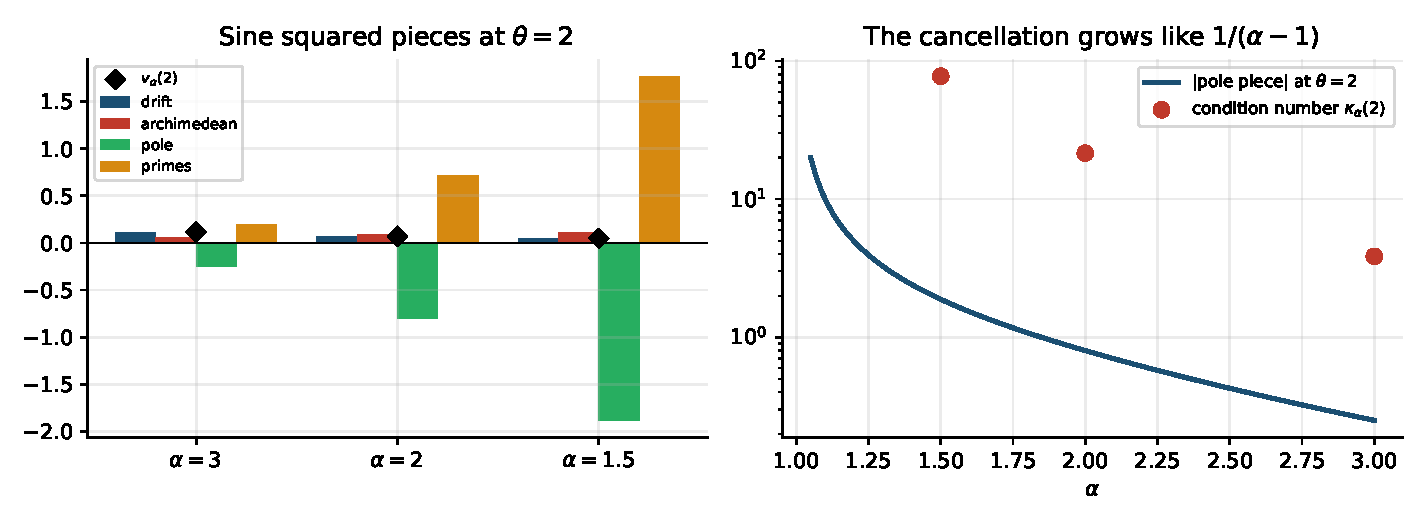
\includegraphics[width=\textwidth]{fig/sin2pieces.pdf}
\caption{Left: the four pieces of the sine squared decomposition at $\theta=2$ for three basepoints, with the bracket $v_\alpha(2)$. Right: the pole piece and the condition number grow like $1/(\alpha-1)$ as the basepoint approaches one.}
\label{fig:ch6:pieces}
\end{figure}

The lemma also prices the prime side. By the prime number theorem the truncation tail satisfies, for fixed $\theta\ne0$,
\[
\sum_{n>N}\frac{\Lambda(n)}{n^\alpha}\big(1-\cos(\theta\log n)\big)\asymp\frac{N^{1-\alpha}}{\alpha-1},
\]
which is $1.4\times10^{-3}$ at $\alpha=1.5$ with $N=2\times10^6$, the size of the errors in Table~\ref{tab:prime}; an absolute error of $10^{-10}$ at $\alpha=1.5$ would need a cutoff $N\approx4\times10^{20}$. For $\alpha\le1$ the series diverges, and the lemma must be read through the regularised pairing of \cite[Chapter 7]{P26} and the explicit formula. At the basepoint one the regularisation is explicit: the pole and prime pieces can be compensated against each other, and Section~\ref{ch:basepoint} converts the resulting L\'evy form of $\xi(1+s)$ term by term into the Thorin density. Near the critical line Selberg's smoothed sum over the primes up to $x^2$ takes the place of the series, and at resolution $\varepsilon$, if no zero lies to the right of the critical line, its error at an ordinate is of order $x^{-\varepsilon}/(\varepsilon^2\log x)$, so that $k$ correct digits need $x\approx10^{k/\varepsilon}$ (Section~\ref{sec:ch10:selberg}). The P\'olya route has none of these costs: its cost per point is polynomial in the height and independent of $\varepsilon$, and at height $200$ it reaches $\varepsilon=0.005$ with about $60$ digits (Section~\ref{sec:ch4:trapezoid}).

\subsection{Consequences for computation}\label{sec:ch6:consequences}

The bracket is the derivative of an argument, $v_\alpha(\theta)=\partial_\theta\arg\xi(\alpha+i\theta)$, because $\partial_\theta\log\xi(\alpha+i\theta)=i(\xi'/\xi)(\alpha+i\theta)$. So the cumulative Thorin mass is an argument,
\[
\mu_\varepsilon\big((0,\theta^2]\big)=\frac1\pi\arg\xi\Big(\frac12+\varepsilon+i\theta\Big),
\]
continued along the line from the real axis, where $\xi>0$. It is computed without quadrature, by accumulating the arguments of quotients of consecutive values of $\xi$, with steps chosen so that each increment can be read from its principal value, a condition checked after the fact rather than guaranteed (Section~\ref{sec:ch4:height200}). Section~\ref{ch:distances} uses it for masses, cell masses, cumulative distances and the mass defect of Proposition~\ref{prop:mass}, and Section~\ref{ch:turing} for the zero count.

The lemma is linear with a nonnegative kernel, so a nonnegative L\'evy input gives a nonnegative Thorin output, and positivity certificates can be posed as linear programs in the sine squared basis \cite[Sections 18.2.8 and 18.2.9]{P26}. For $\xi$ the only negative part of the input $xL(dx)$ is the pole density $-e^{-(\alpha-1)x}dx$, so a certificate must show that the positive pieces dominate the pole piece at every $\theta$. For $\alpha>1$ they do (Theorem~\ref{thm:poisson}), although the proof goes through the zeros and not through the input. For $\tfrac12<\alpha\le1$, where the lemma is read through the regularised pairing, domination at every basepoint is Lagarias's criterion, that is RH, and Section~\ref{sec:ch10:positivity} states RH as a domination of the same kind at the centre, Weil's criterion on variograms. Beurling generalised prime systems, in which the sign of the input is controlled by construction, are among the open computations of Section~\ref{sec:open:calib}.

The lemma also supplies an exact consistency check at $\alpha=\tfrac12$, where the constant parts of the pole and prime pieces diverge and are continued analytically. The constant part $1/(\alpha-1)$ of the pole piece continues to $-2$ and enters with a minus sign; the constant part $-\zeta'/\zeta(\alpha)$ of the prime piece continues to $-\zeta'/\zeta(\tfrac12)$; and the gamma factor contributes the archimedean constant of \cite[Section 6.8]{P26}, $C_\Gamma=\tfrac12\log\pi-\tfrac12\psi(\tfrac14)-2=0.6860917096$, which is minus the logarithmic derivative of $s\pi^{-s/2}\Gamma(s/2)$ at $s=\tfrac12$. They sum to
\[
C_\Gamma+2-\frac{\zeta'}{\zeta}\Big(\frac12\Big)=0,
\]
which is equivalent to $\xi'(\tfrac12)=0$, because $\xi'/\xi(s)=1/s+1/(s-1)-\tfrac12\log\pi+\tfrac12\psi(s/2)+\zeta'/\zeta(s)$ and $1/s+1/(s-1)$ vanishes at $s=\tfrac12$. Any implementation of the sine squared route can be tested against this identity, and the P\'olya route satisfies its analogue automatically, since
\[
\xi'\big(\tfrac12\big)=\int_{\mathbb R}u\,\Phi(u)\,du=0
\]
by the evenness of $\Phi$.

\section{Distances to the discrete measure implied by RH}\label{ch:distances}



On a window where the zeros are known, the Thorin measure $\mu_\varepsilon$ computed by the P\'olya route can be compared with $U_{\RH}$ directly (Section~\ref{sec:ch6:measure}), and how close the two are depends on the metric.

Fix $\Theta=200$ and the window $E=(0,\Theta^2]$ in $z$, equivalently $(0,\Theta]$ in $\theta$. The window contains $79$ zeros, all simple and on the line, and $\Theta$ is not an ordinate, since $\gamma_{80}=201.2648$ (Section~\ref{sec:ch4:height200}). For a signed measure $\nu$ on $E$ write $\tv{\nu}=|\nu|(E)$, and write $M_\varepsilon(\theta)=\mu_\varepsilon((0,\theta^2])$ for the cumulative mass.

\subsection{Total variation at matched resolution}\label{sec:ch7:matched}

A smooth approximation to a sum of point masses never converges to it in total variation.

\begin{proposition}\label{prop:raw}
If $\nu\ge0$ is absolutely continuous and $U$ is purely atomic with $N$ unit atoms in $E$, then $\tv{\nu-U}=\nu(E)+N$.
\end{proposition}

\begin{proof}
Let $A$ be the finite set of atoms. Then $\nu(A)=0$, so $|\nu-U|(A)=U(A)=N$ and $|\nu-U|(E\setminus A)=\nu(E\setminus A)=\nu(E)$.
\end{proof}

The Thorin measure is positive on $E$, where its density has minimum $0.0147\,\varepsilon$ (Section~\ref{sec:ch6:measure}), so $\tv{\mu_\varepsilon-U_{\RH}}=\mu_\varepsilon(E)+79\approx158$ for every $\varepsilon$. Total variation becomes informative only after both measures have been brought to the same resolution, or summed over cells.

By Proposition~\ref{prop:struct} the object to compare with $\mu_\varepsilon$ is the Poisson smoothing of the RH measure at the same resolution, and we write $d_{\rm match}(\varepsilon)=\tv{\mu_\varepsilon-P_\varepsilon*U^\pm_{\RH}}$ for the matched distance. Under RH the two measures coincide and $d_{\rm match}(\varepsilon)=0$, so a computation of the matched distance measures its own error unless some zero is off the line.

A computation replaces $U^\pm_{\RH}$ by a model $\widetilde U$, which we build from the first $1700$ ordinates, computed with \texttt{mpmath} \cite{mpmath}, and from the smooth density $\pi^{-1}\vartheta'(t)\,dt$ of the Riemann Siegel theta function beyond the Gram point $T_*=g_{1699}=2197.8796$ of Section~\ref{sec:ch5:turing}, at which $\vartheta(T_*)/\pi+1=1700$, each with its reflection. We write $\tilde d_{\rm match}(\varepsilon)=\tv{\mu_\varepsilon-P_\varepsilon*\widetilde U}$ for the matched distance against the model. Since $\gamma_{1700}=2197.2587<T_*<\gamma_{1701}=2198.6875$, we have $N(T_*)=\vartheta(T_*)/\pi+1$, so the boundary term vanishes when $\int_{T_*}^\infty P_\varepsilon(\theta-t)\,d\big(N(t)-\vartheta(t)/\pi-1\big)$ is integrated by parts, and the error of the tail model is at most of order $\varepsilon/T_*^2$ per unit length. The observed floor is far smaller: $\tilde d_{\rm match}(\varepsilon)=3.66\times10^{-9}\,\varepsilon$ at every resolution from $\varepsilon=1$ to $\varepsilon=0.005$ (Table~\ref{tab:tv}), that is $1.8\times10^{-11}\,\varepsilon$ per unit length. The exact proportionality to $\varepsilon$ identifies the floor as the residual of the tail model; it is an observed value, not a bound for $d_{\rm match}(\varepsilon)$: such a bound would need certified bounds on the error of the tail model and on the evaluation of $\mu_\varepsilon$. The densities that enter the comparison are stored in double precision.

\begin{table}[t]
\centering\small\setlength{\tabcolsep}{4pt}
\begin{tabular}{rrrrrrrr}
\toprule
$\varepsilon$ & mass & raw TV & matched TV & sup diff & cell TV & $L^1$ in $\theta$ & $W_\varepsilon(0.01)$\\
\midrule
1 & 79.36738 & 158.37 & $3.66\times10^{-9}$ & $1.9\times10^{-11}$ & 4.992 & 59.23 & 0.29504\\
0.5 & 79.19417 & 158.19 & $1.83\times10^{-9}$ & $9.6\times10^{-12}$ & 2.655 & 41.86 & 0.22362\\
0.25 & 79.09887 & 158.10 & $9.14\times10^{-10}$ & $4.8\times10^{-12}$ & 1.351 & 28.77 & 0.18698\\
0.1 & 79.03977 & 158.04 & $3.66\times10^{-10}$ & $1.9\times10^{-12}$ & 0.5431 & 16.01 & 0.16469\\
0.05 & 79.01990 & 158.02 & $1.83\times10^{-10}$ & $9.6\times10^{-13}$ & 0.2718 & 9.737 & 0.15721\\
0.02 & 79.00796 & 158.01 & $7.31\times10^{-11}$ & $3.8\times10^{-13}$ & 0.1087 & 4.816 & 0.15270\\
0.01 & 79.00398 & 158.00 & $3.66\times10^{-11}$ & $2.0\times10^{-13}$ & 0.05437 & 2.756 & 0.15120\\
0.005 & 79.00199 & 158.00 & $1.83\times10^{-11}$ & $1.5\times10^{-13}$ & 0.02718 & 1.553 & 0.15045\\
\midrule
RH & 79 & 0 & 0 & 0 & 0 & 0 & 0.14970\\
\bottomrule
\end{tabular}
\caption{Distances between the P\'olya computed Thorin measure $\mu_\varepsilon$ and $U_{\RH}$ on $0<z\le200^2$. Mass is $M_\varepsilon(200)$. Raw TV is $\tv{\mu_\varepsilon-U_{\RH}}$, forced to equal mass plus $79$ by Proposition~\ref{prop:raw}. Matched TV is $\tilde d_{\rm match}(\varepsilon)=\tv{\mu_\varepsilon-P_\varepsilon*\widetilde U}$, and sup diff is the maximum of $|\rho_\varepsilon-P_\varepsilon*\widetilde U|$ over $0<\theta\le200$. Cell TV is $d_{\rm cell}(\varepsilon)$, $L^1$ in $\theta$ is $\int_0^{200}|M_\varepsilon-N|\,d\theta$, and $W_\varepsilon(0.01)$ is the smoothed heat trace at $t=0.01$, with the value from the zeros in the last row.}
\label{tab:tv}
\end{table}

\subsection{Cumulative distances and extrapolation in the resolution}\label{sec:ch7:cumulative}

The total mass is the simplest quantity to compare, since $U_{\RH}(E)=N(\Theta)=79$. By Section~\ref{sec:ch6:consequences} it is an argument, $\mu_\varepsilon(E)=\pi^{-1}\arg\xi(\tfrac12+\varepsilon+i\Theta)$, continued from $\arg\xi(\tfrac12+\varepsilon)=0$.

\begin{proposition}\label{prop:mass}
Suppose $\Theta$ is not an ordinate and every zero with $0<\im\rho\le\Theta$ lies on the line. Then
\[
\mu_\varepsilon\big((0,\Theta^2]\big)=N(\Theta)-\frac{\varepsilon}{\pi}\,\frac{\Xi'(\Theta)}{\Xi(\Theta)}+O(\varepsilon^2),\qquad \varepsilon\downarrow0.
\]
\end{proposition}

\begin{proof}
Let $\sigma_1>1$. By hypothesis, and because $\xi$ is positive on the real axis, $\xi$ has no zero in the closed rectangle with vertices $\tfrac12+\varepsilon$, $\sigma_1$, $\sigma_1+i\Theta$ and $\tfrac12+\varepsilon+i\Theta$. So the change of $\arg\xi$ up its left side, which is $\pi\mu_\varepsilon((0,\Theta^2])$, equals the change along the path $\tfrac12+\varepsilon\to\sigma_1\to\sigma_1+i\Theta\to\tfrac12+\varepsilon+i\Theta$. The classical formula $\pi N(\Theta)=\Delta\arg\xi$ along $\tfrac12\to\sigma_1\to\sigma_1+i\Theta\to\tfrac12+i\Theta$ \cite[Section 9.3]{Titchmarsh} differs from it only by the segment from $\tfrac12+\varepsilon+i\Theta$ to $\tfrac12+i\Theta$, since $\arg\xi$ is constant on the real axis. Put $h(\varepsilon)=\xi(\tfrac12+\varepsilon+i\Theta)$. Since $h(0)=\Xi(\Theta)\ne0$, a branch of $\arg h$ is real analytic near $\varepsilon=0$, and
\[
\pi\mu_\varepsilon\big((0,\Theta^2]\big)=\pi N(\Theta)+\arg h(\varepsilon)-\arg h(0)=\pi N(\Theta)+\varepsilon\,\im\frac{\xi'}{\xi}\Big(\frac12+i\Theta\Big)+O(\varepsilon^2).
\]
From $\frac{d}{d\theta}\Xi(\theta)=i\xi'(\tfrac12+i\theta)$ we get $(\xi'/\xi)(\tfrac12+i\Theta)=-i\,\Xi'(\Theta)/\Xi(\Theta)$, and $\Xi'/\Xi$ is real, so the coefficient of $\varepsilon$ is $-\Xi'(\Theta)/\Xi(\Theta)$.
\end{proof}

\begin{remark}\label{rem:ch7:cubic}
The remainder in Proposition~\ref{prop:mass} is in fact $O(\varepsilon^3)$: $\xi(s)=\xi(1-s)$ and the reality of $\xi$ on the real axis give $h(-\varepsilon)=\overline{h(\varepsilon)}$, so $\arg h(\varepsilon)-\arg h(0)$ is odd in $\varepsilon$ and its expansion has no term in $\varepsilon^2$.
\end{remark}

Choosing $\Theta$ midway between zeros makes the correction small, and adding it recovers $N(\Theta)$ up to $O(\varepsilon^3)$; Proposition~\ref{prop:zerodensity} makes the recovery exact. At $\Theta=200$ the P\'olya route gives $\Xi'(200)/\Xi(200)=-1.2506879$, so the proposition predicts $\mu_\varepsilon(E)-79=-\varepsilon\,\Xi'(200)/(\pi\,\Xi(200))+O(\varepsilon^3)$, with $-\Xi'(200)/(\pi\,\Xi(200))=0.3981063$; the observed $(\mu_\varepsilon(E)-79)/\varepsilon$ is $0.398105$ at $\varepsilon=0.005$ and $0.398102$ at $\varepsilon=0.01$. Figure~\ref{fig:cumulative} compares $M_\varepsilon$ with the counting function of $U_{\RH}$ across the window.

\begin{figure}[t]
\centering
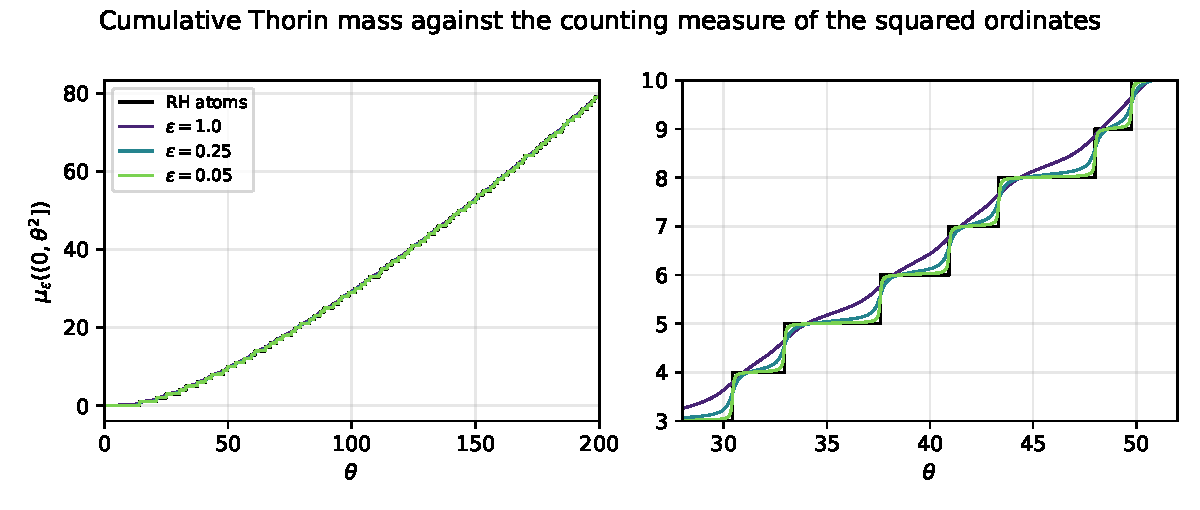
\includegraphics[width=0.95\textwidth]{fig/cumulative.pdf}
\caption{Cumulative Thorin mass $\mu_\varepsilon((0,\theta^2])=\pi^{-1}\arg\xi(\tfrac12+\varepsilon+i\theta)$ at $\varepsilon=1$, $0.25$ and $0.05$ against the counting function of $U_{\RH}$, on the whole window (left) and on $28\le\theta\le52$ (right).}
\label{fig:cumulative}
\end{figure}

Summing over cells gives a distance that resolves the individual zeros. Let $b_0=0$, $b_k=(\gamma_k+\gamma_{k+1})/2$ for $1\le k\le78$ and $b_{79}=\Theta$, and let $C_k=(b_{k-1},b_k]$. The cell masses $\mu_\varepsilon(C_k)=M_\varepsilon(b_k)-M_\varepsilon(b_{k-1})$ are differences of the argument, and the coarse grained distance
\[
d_{\rm cell}(\varepsilon)=\sum_k|\mu_\varepsilon(C_k)-1|
\]
is the total variation distance between the images of $\mu_\varepsilon$ and $U_{\RH}$ under the map sending each cell to its atom. No $b_k$ is an ordinate, so Proposition~\ref{prop:mass} applies at both ends of every cell, with $\Xi'(0)=0$ at $b_0$, and with the remainder of Remark~\ref{rem:ch7:cubic} gives $\mu_\varepsilon(C_k)-1=-(\varepsilon/\pi)\big[\Xi'/\Xi(b_k)-\Xi'/\Xi(b_{k-1})\big]+O(\varepsilon^3)$. Hence $d_{\rm cell}(\varepsilon)=\kappa_{\rm cell}\,\varepsilon+O(\varepsilon^3)$, where $\kappa_{\rm cell}=\pi^{-1}\sum_k|\Xi'/\Xi(b_k)-\Xi'/\Xi(b_{k-1})|$, the cell constant of this window, is $5.43665$, and every cell mass lies in $[0.99888,1.00126]$ at $\varepsilon=0.005$. Section~\ref{ch:spacing} reads this constant as a statistic of the irregularity of the spacings.

The $L^1$ distance $\int_0^\Theta|M_\varepsilon(\theta)-N(\theta)|\,d\theta$ between the cumulative mass and the counting function is a transport distance, and because of the Cauchy tails it behaves like $\varepsilon\log(1/\varepsilon)$: it is $1.55$ in $\theta$ and $360$ in $z$ at $\varepsilon=0.005$, and Section~\ref{sec:ch9:mass} derives the rate. The heat trace $W(t)=\int e^{-tz}U_{\RH}(dz)$ is approximated by $W_\varepsilon(t)=\int_0^\infty e^{-t\theta^2}\rho_\varepsilon(\theta)\,d\theta=\int e^{-tz}\mu_\varepsilon(dz)$. At $t=0.01$ the zeros give $W=0.1496980112538$ (Table~\ref{tab:ch2:W}), while $W_\varepsilon(0.01)=0.1504500280599$, $0.1512017825455$ and $0.1527045050533$ at $\varepsilon=0.005$, $0.01$ and $0.02$, again with error linear in $\varepsilon$.

The mass and the heat trace are smooth in $\varepsilon$ at $\varepsilon=0$, so Richardson extrapolation applies to them: the mass by Proposition~\ref{prop:mass}, and the heat trace because by Proposition~\ref{prop:struct} it is a sum over the zeros of Poisson integrals of the Gaussian $e^{-t\theta^2}$. The combination $2\mu_{0.005}(E)-\mu_{0.01}(E)$ equals $79+3.2\times10^{-8}$, against a raw defect of $2.0\times10^{-3}$. For the heat trace the error $7.5\times10^{-4}$ of $W_{0.005}(0.01)$ falls to $2.6\times10^{-7}$ after one Richardson step ($\varepsilon=0.005$ and $0.01$) and to $1.7\times10^{-10}$ after two (adding $\varepsilon=0.02$). Without extrapolation the same accuracy would need $\varepsilon\approx8\times10^{-8}$ for the mass, and $\varepsilon\approx2\times10^{-6}$ and $10^{-9}$ for the heat trace.


\section{What an off line zero would do}\label{ch:offline}



The distances of Section~\ref{ch:distances} compare $\mu_\varepsilon$ with $U_{\RH}$ on a window where the zeros are known to lie on the line, and there the matched distance leaves only a numerical floor. How each distance would change if a zero left the line can be computed in closed form, because by Proposition~\ref{prop:struct} an off line zero at distance $\delta$ from the line enters the Thorin density, together with its reflection in the line, only through the kernels $P_{\varepsilon+\delta}+P_{\varepsilon-\delta}$ at its ordinate, the second of which is negative once $\varepsilon<\delta$. Proposition~\ref{prop:signature} computes the effect for a displacement that keeps the count, for a pair missing from a list of line zeros, and for the negative mass of a displaced zero. Together the three signatures show that an off line zero is most visible at resolutions comparable to its distance from the line, a theme that returns in Section~\ref{ch:finite}. Read against the floor of the matched distance, they give detection thresholds below height $200$ and a calibration of the method above it.

\subsection{Three signatures of an off line zero}\label{sec:ch8:signatures}

Off line zeros come in pairs $\tfrac12\pm\delta+i\gamma$ with $0<\delta<\tfrac12$, together with their conjugates, and near $\gamma$ a pair contributes $P_{\varepsilon+\delta}+P_{\varepsilon-\delta}$ to $\rho_\varepsilon$ where two line zeros would contribute $2P_\varepsilon$. A displacement that keeps the count $N(T)$ therefore moves two line zeros at height $\gamma$ to such a pair, as a double zero does at a collision in the de Bruijn Newman flow (Section~\ref{ch:dbn}). Parts (i) and (iii) of Proposition~\ref{prop:signature} are normalised per displaced zero, and part (ii) per pair.

\begin{proposition}\label{prop:signature}
Let $\varepsilon>0$ and $0<\delta<\tfrac12$; when $\delta=\varepsilon$, $P_0$ denotes the unit point mass at the origin.
\begin{enumerate}
\item[(i)] (Displaced zeros, same count.) If two line zeros at height $\gamma$ are replaced by the quadruple $\tfrac12\pm\delta\pm i\gamma$, the density near $\gamma$ changes by $2g$, where $g=\tfrac12(P_{\varepsilon+\delta}+P_{\varepsilon-\delta})-P_\varepsilon$ is the change per displaced zero, and
\[
\tv{g}=\frac{3\sqrt3}{4\pi}\Big(\frac\delta\varepsilon\Big)^2+O\Big(\frac{\delta^4}{\varepsilon^4}\Big),\qquad \delta<\varepsilon .
\]
\item[(ii)] (Pair omitted from the list.) If a pair at $\tfrac12\pm\delta+i\gamma$ exists but a list of line zeros omits it, the difference is $P_{\varepsilon+\delta}+P_{\varepsilon-\delta}$ and
\[
\tv{P_{\varepsilon+\delta}+P_{\varepsilon-\delta}}=\begin{cases}2,&\delta\le\varepsilon,\\[2pt] \dfrac8\pi\arctan\sqrt{\dfrac{\delta+\varepsilon}{\delta-\varepsilon}}-2,&\delta>\varepsilon.\end{cases}
\]
\item[(iii)] (Negative mass.) For $\delta>\varepsilon$ the negative part of $\tfrac12(P_{\varepsilon+\delta}+P_{\varepsilon-\delta})$, the density of one displaced zero, has mass \[\frac2\pi\arctan\sqrt{\frac{\delta+\varepsilon}{\delta-\varepsilon}}-\frac12=\frac{\varepsilon}{\pi\delta}+O\Big(\frac{\varepsilon^3}{\delta^3}\Big).\]
\end{enumerate}
\end{proposition}

\begin{proof}
(i) Taylor expansion in $\delta$ gives $g=\tfrac{\delta^2}{2}\partial_a^2P_a|_{a=\varepsilon}+O(\delta^4)$ \cite[Proposition 19.7]{P26}, with a remainder of $L^1$ norm $O(\delta^4/\varepsilon^4)$. Since $\partial_a^2P_a(x)=(2a/\pi)(a^2-3x^2)/(a^2+x^2)^3$, the substitution $x=\varepsilon v$ gives $\partial_a^2P_a|_{a=\varepsilon}=2(1-3v^2)/(\pi\varepsilon^3(1+v^2)^3)$ and $dx=\varepsilon\,dv$. The function $(1-3v^2)/(1+v^2)^3$ is the derivative of $v/(1+v^2)^2$, whose total variation is four times its maximum $9/(16\sqrt3)$, that is $3\sqrt3/4$, so the $L^1$ norm of $\partial_a^2P_a$ at $a=\varepsilon$ is $(2/(\pi\varepsilon^2))\cdot3\sqrt3/4=\frac{3\sqrt3}{2\pi\varepsilon^2}$, and multiplying by $\delta^2/2$ gives (i).
(ii) For $\delta\le\varepsilon$ both kernels are nonnegative with mass one. For $\delta>\varepsilon$ put $a=\delta+\varepsilon$, $b=\delta-\varepsilon$, so the difference is $P_a-P_b$, which is negative exactly on $|x|<\sqrt{ab}$. Integrating, $\tv{P_a-P_b}=\frac4\pi[\arctan\sqrt{a/b}-\arctan\sqrt{b/a}]$, and $\arctan y+\arctan(1/y)=\pi/2$.
(iii) $P_a-P_b$ has total mass zero, so its negative part is half its norm; halve again for the factor $\tfrac12$.
\end{proof}

With $\varepsilon/\delta=\sin\phi$ one has $\arctan\sqrt{(\delta+\varepsilon)/(\delta-\varepsilon)}=\pi/4+\phi/2$, so for $\delta>\varepsilon$ the norm in (ii) is $(4/\pi)\arcsin(\varepsilon/\delta)$ and the mass in (iii) is $(1/\pi)\arcsin(\varepsilon/\delta)$. In part (i) the list is correct in number but two of its zeros have left the line, and the density differs from the Poisson smoothing of the list by $2g$, which to leading order is $\delta^2\partial_a^2P_a$ at $a=\varepsilon$, quadratic in the displacement. In part (ii) the list omits the pair; the difference is of order one while the resolution is coarser than the displacement, and fades like $4\varepsilon/(\pi\delta)$ once it is finer. Part (iii) bounds the negative mass that a displaced zero can contribute, which also fades like $\varepsilon/\delta$. Figure~\ref{fig:sensitivity} plots the three signatures.

\begin{figure}[t]
\centering
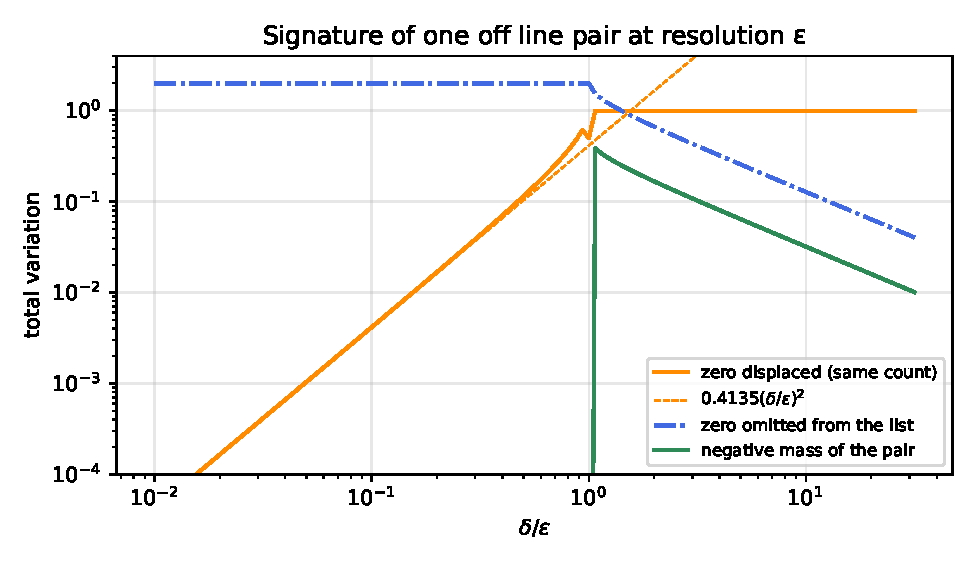
\includegraphics[width=0.7\textwidth]{fig/sensitivity.pdf}
\caption{The three signatures of Proposition~\ref{prop:signature} as functions of $\delta/\varepsilon$: $\tv{g}$ per displaced zero (part (i)), with its leading term $0.4135(\delta/\varepsilon)^2=(3\sqrt3/(4\pi))(\delta/\varepsilon)^2$ dashed; the total variation of an omitted pair (part (ii)); and the negative mass per displaced zero (part (iii)). For $\delta>\varepsilon$, outside the range of part (i), the kernels of a displaced zero have total mass zero and curve (i) is flat at $1$.}
\label{fig:sensitivity}
\end{figure}

\subsection{Calibration of the matched distance}\label{sec:ch8:calibration}

Proposition~\ref{prop:signature} converts the matched distance of Section~\ref{ch:distances} into detection thresholds. By part (ii), a computed matched distance $\tilde d_{\rm match}(\varepsilon)$ of at most $3.7\times10^{-9}\,\varepsilon$ excludes any omitted pair with ordinate in $(0,200)$: such a pair contributes total variation $(4/\pi)\arcsin(\varepsilon/\delta)$, or $2$ if $\delta\le\varepsilon$, less only the part of its kernels outside the window. By part (i), a displaced pair that keeps the count adds $2g$ to a difference whose norm is the floor $\tilde d_{\rm match}(\varepsilon)$, so by the triangle inequality the matched distance rises above the floor as soon as $\tv{g}>\tilde d_{\rm match}(\varepsilon)$, that is, to leading order, once $\delta$ exceeds
\begin{equation}\label{eq:ch8:threshold}
\delta_{\min}(\varepsilon)=\varepsilon\Big(\frac{4\pi\,\tilde d_{\rm match}(\varepsilon)}{3\sqrt3}\Big)^{1/2}.
\end{equation}
With the floors of Table~\ref{tab:tv} this threshold is $3.3\times10^{-5}$ at $\varepsilon=0.5$, $1.1\times10^{-6}$ at $\varepsilon=0.05$ and $3.3\times10^{-8}$ at $\varepsilon=0.005$.

The threshold \eqref{eq:ch8:threshold} is the square root law of \cite[Proposition 19.7]{P26}: the signature grows like the square of the displacement, so the smallest detectable displacement falls like the square root of the achievable distance. The prime side calibration of \cite[Section 19.3.6]{P26} obeys the same law and reaches $\delta\approx0.05$ at $\varepsilon=2$. What changes is the reach: the P\'olya route evaluates $\rho_\varepsilon$ at small $\varepsilon$ to about $60$ digits below height $200$ (Section~\ref{sec:ch4:trapezoid}), so the floor is set by the tail model for the zero list (Section~\ref{sec:ch7:matched}) rather than by the evaluator, whereas the prime side is limited by the truncation of Table~\ref{tab:prime}. A positivity test sees less than the matched distance: only the negative part of the whole density, which by part (iii) is at most of order $\varepsilon/\delta$ per displaced zero and which the kernels of the neighbouring zeros can cancel entirely (Section~\ref{ch:finite}). Section~\ref{ch:almost} bounds the mass of the negative part of the density below a given height by the number of zeros to the right of the basepoint and, through zero density estimates, shows with no hypothesis that it is a vanishing fraction of the positive part.

These thresholds concern zeros below height $200$, where the argument principle count is already decisive, and their use is to calibrate the method above the verified window. There the cost per point of the P\'olya route grows with the height (Section~\ref{sec:ch6:measure}), and the count itself must come from the argument of $\xi$, which Section~\ref{ch:turing} reads from the Thorin mass (Proposition~\ref{prop:zerodensity}).

\section{Counting zeros with the Thorin measure}\label{ch:turing}
\label{sec:turing}


Turing's method certifies the count $N(T)$ without evaluating $\zeta$ off the critical line, from the sign changes of $Z$ and an explicit bound on the integral of $S$, where $\pi S(t)=\arg\zeta(\tfrac12+it)$; Backlund's method, which it replaced, bounds the argument of $\zeta$ along a horizontal segment off the line (Section~\ref{sec:ch5:turing}). Without the assumption of Proposition~\ref{prop:mass} that the zeros below the window lie on the line, the argument principle gives at every resolution an exact identity for $N(T)$ and for the number $\nu(\tfrac12+\varepsilon,T)$ of zeros to the right of the line of evaluation, so that off line zeros are counted and not only detected. At $\varepsilon=\tfrac12$ the identity is Backlund's count with the vertical side on $\re s=1$.

\subsection{The cumulative Thorin mass as a smoothed counting function}\label{sec:ch9:mass}

Recall that $M_\varepsilon(\theta)=\mu_\varepsilon((0,\theta^2])=\pi^{-1}\arg\xi(\tfrac12+\varepsilon+i\theta)$, with the argument continued along the line $\re s=\tfrac12+\varepsilon$ from $\theta=0$, where $\xi>0$ (Sections~\ref{sec:ch6:consequences} and \ref{ch:distances}). Since $\xi(s)=\tfrac12s(s-1)\pi^{-s/2}\Gamma(s/2)\zeta(s)$, the mass splits as
\[
M_\varepsilon(\theta)=N^{\rm sm}_\varepsilon(\theta)+S_\varepsilon(\theta),\qquad S_\varepsilon(\theta)=\frac1\pi\arg\zeta\Big(\frac12+\varepsilon+i\theta\Big),
\]
where, with $s=\tfrac12+\varepsilon+i\theta$ and $\theta>0$, the smooth part $N^{\rm sm}_\varepsilon(\theta)=\pi^{-1}\big[\arg s+\arg(s-1)+\im\log\Gamma(\tfrac14+\tfrac\varepsilon2+\tfrac{i\theta}2)-\tfrac\theta2\log\pi\big]$ comes from $s(s-1)\pi^{-s/2}\Gamma(s/2)$, with the principal arguments of $s$ and $s-1$, which lie in $(0,\pi)$, and the branch of $\log\Gamma$ that is real on the positive axis. Thus $S_\varepsilon$ is $\pi^{-1}\arg\zeta$ continued along the vertical line from $S_\varepsilon(0+)=-1$ if $0<\varepsilon<\tfrac12$, when $\arg(s-1)\to\pi$ as $\theta\downarrow0$, and from $S_\varepsilon(0+)=0$ if $\varepsilon>\tfrac12$.

As $\varepsilon\downarrow0$, $N^{\rm sm}_\varepsilon\to\vartheta/\pi+1$, where $\vartheta(\theta)=\im\log\Gamma(\tfrac14+\tfrac{i\theta}2)-\tfrac\theta2\log\pi$ is the Riemann Siegel theta function, and for $\theta$ not an ordinate Proposition~\ref{prop:zerodensity} below gives $M_\varepsilon(\theta)\to N(\theta)-2\nu(\tfrac12,\theta)$, where $\nu(\sigma,\theta)$ counts the zeros with real part greater than $\sigma$ and ordinate in $(0,\theta]$ (Section~\ref{ch:intro}). When no zero below height $\theta$ lies to the right of the critical line, the limit is therefore the Riemann von Mangoldt formula $N(\theta)=\vartheta(\theta)/\pi+1+S(\theta)$ \cite[Section 9.3]{Titchmarsh}.

Integrating Proposition~\ref{prop:struct} in $\theta$ writes $M_\varepsilon$ as a sum of Cauchy steps. Under RH, for $\theta\ge0$,
\begin{gather*}
M_\varepsilon(\theta)=\sum_{\gamma>0}\big[F_\varepsilon(\theta-\gamma)-F_\varepsilon(-\gamma)+F_\varepsilon(\theta+\gamma)-F_\varepsilon(\gamma)\big],\\
F_\varepsilon(x)=\frac12+\frac1\pi\arctan\frac x\varepsilon ,
\end{gather*}
with the sum over all positive ordinates. Since $F_\varepsilon(-\gamma)+F_\varepsilon(\gamma)=1$, this says that $M_\varepsilon=P_\varepsilon*\tilde N$, where $\tilde N$ is the odd extension of $N$. As $\vartheta$ is odd, $S_\varepsilon$ is then the Poisson average of the odd extension of $S$ up to an explicit smooth function. If only the zeros below height $T+B$ are known to lie on the line, the display holds on $[0,T]$ up to an error of order $\varepsilon\delta^2/B^3$ for each off line pair above $T+B$ at distance $\delta$ from the line, counted as a double ordinate, because $P_{\varepsilon+\delta}(x)+P_{\varepsilon-\delta}(x)-2P_\varepsilon(x)=-6\varepsilon\delta^2/(\pi x^4)+O(x^{-6})$.

For a single step,
\begin{align*}
\int_{-L}^{L}\big|F_\varepsilon(x)-\mathbf 1_{x\ge0}\big|\,dx&=\frac2\pi\Big[L\arctan\frac\varepsilon L+\frac\varepsilon2\log\Big(1+\frac{L^2}{\varepsilon^2}\Big)\Big]\\
&=\frac{2\varepsilon}\pi\Big(\log\frac L\varepsilon+1\Big)+O\Big(\frac{\varepsilon^3}{L^2}\Big),
\end{align*}
which explains the $\varepsilon\log(1/\varepsilon)$ rate of the $L^1$ distance in Table~\ref{tab:tv}. Taking half of it on each side of each of the $79$ zeros below height $200$, with $L$ the half gap on that side, gives $1.61$ at $\varepsilon=0.005$, against the computed $1.55$; the difference comes from the tails of the other steps.

\subsection{A Littlewood identity and the zero density}\label{sec:ch9:density}

\begin{proposition}\label{prop:littlewood}
Let $T>0$. For every $\varepsilon>0$ such that $\xi$ has no zero on the segment from $\tfrac12+\varepsilon$ to $\tfrac12+\varepsilon+iT$,
\[
\pi M_\varepsilon(T)=\frac{\partial}{\partial\varepsilon}\int_0^T\log\Big|\xi\Big(\frac12+\varepsilon+it\Big)\Big|\,dt,
\]
and for every $\varepsilon>0$
\[
\int_0^T\log\Big|\xi\Big(\frac12+\varepsilon+it\Big)\Big|\,dt=\int_0^T\log\Big|\xi\Big(\frac12+it\Big)\Big|\,dt+\pi\int_0^\varepsilon M_{\varepsilon'}(T)\,d\varepsilon' .
\]
\end{proposition}

\begin{proof}
Since $\partial_\sigma\log|\xi(\sigma+it)|=\re(\xi'/\xi)(\sigma+it)=v_\sigma(t)$ and $v_\sigma(t)=\partial_t\arg\xi(\sigma+it)$, we have $M_\varepsilon(T)=\pi^{-1}\int_0^Tv_{1/2+\varepsilon}(t)\,dt$, and when no zero lies on the segment, differentiation under the integral gives the first identity. The integral $I(\varepsilon)$ on the left of the second is continuous on $[0,\infty)$, because the logarithmic singularities at the zeros are integrable uniformly in $\varepsilon$, and continuously differentiable except at the finitely many $\varepsilon'$ at which the segment meets a zero. There $I'$ jumps by $2\pi$ for each zero met at an interior point of the segment, since $\int_{-c}^{c}a\,du/(a^2+u^2)\to\pm\pi$ as $a\to0\pm$. So $I$ is absolutely continuous, and $I(\varepsilon)-I(0)=\int_0^\varepsilon I'(\varepsilon')\,d\varepsilon'$ is the second identity.
\end{proof}

The jump of $2\pi$ in the slope $\pi M_\varepsilon(T)$ when the line crosses a zero is the term $2\nu$ of Proposition~\ref{prop:zerodensity} below. Littlewood's lemma \cite[Section 9.9]{Titchmarsh} is the same Cauchy Riemann identity with the argument taken along a path through $\re s=2$; the two arguments differ by $2\pi\nu(\tfrac12+\varepsilon,T)$, and Exercise~\ref{ex:ch9:littlewood} derives the lemma from the two propositions. Let $\tau_\varepsilon(T)=\pi^{-1}\Delta\arg\xi$ along the horizontal segment from $\tfrac12+\varepsilon+iT$ to $\tfrac12+iT$.

\begin{proposition}\label{prop:zerodensity}
Let $\varepsilon>0$ and $T>0$, with $T$ not an ordinate and no zero of $\xi$ on the segment from $\tfrac12+\varepsilon$ to $\tfrac12+\varepsilon+iT$. Then
\[
M_\varepsilon(T)+\tau_\varepsilon(T)=N(T)-2\,\nu\Big(\frac12+\varepsilon,T\Big).
\]
The segment condition holds at $\varepsilon=\tfrac12$, and $\nu(1,T)=0$, which gives the unconditional count $N(T)=M_{1/2}(T)+\tau_{1/2}(T)$, so that $\nu(\tfrac12+\varepsilon,T)=\tfrac12\big[N(T)-M_\varepsilon(T)-\tau_\varepsilon(T)\big]$ for every $\varepsilon$ satisfying the hypotheses.
\end{proposition}

\begin{proof}
Let $\sigma_1>1$. Write $\Delta_{\rm right}$ for the change of $\arg\xi$ along the segment from $\sigma_1$ to $\sigma_1+iT$, and $\Delta_{\rm top}(a\to b)$ for its change along the segment from $a+iT$ to $b+iT$. The argument principle on the rectangle $[\tfrac12+\varepsilon,\sigma_1]\times[0,T]$, on whose bottom edge $\xi$ is positive, gives $\Delta_{\rm right}+\Delta_{\rm top}(\sigma_1\to\tfrac12+\varepsilon)-\pi M_\varepsilon(T)=2\pi\nu(\tfrac12+\varepsilon,T)$. Subtracting this from the classical formula $\pi N(T)=\Delta_{\rm right}+\Delta_{\rm top}(\sigma_1\to\tfrac12)$ \cite[Section 9.3]{Titchmarsh} leaves $\Delta_{\rm top}(\tfrac12+\varepsilon\to\tfrac12)+\pi M_\varepsilon(T)=\pi N(T)-2\pi\nu(\tfrac12+\varepsilon,T)$, and $\Delta_{\rm top}(\tfrac12+\varepsilon\to\tfrac12)=\pi\tau_\varepsilon(T)$. At $\varepsilon=\tfrac12$ the segment lies on $\re s=1$, where $\zeta$ has no zeros, and $\nu(1,T)=0$ because the Euler product has no zeros in $\re s>1$.
\end{proof}

Half the difference of $M_\varepsilon(T)+\tau_\varepsilon(T)$ at two resolutions counts the zeros in the strip between the two lines. The factor two comes from the functional equation: a zero $\tfrac12+\delta+i\gamma$ with $\delta>\varepsilon$ and its partner $\tfrac12-\delta+i\gamma$ add $2$ to $N(T)$ and $1$ to $\nu(\tfrac12+\varepsilon,T)$, hence nothing to $M_\varepsilon(T)+\tau_\varepsilon(T)$, whereas two zeros on the line at the same ordinate add $2$. In the density the pair enters through the kernels $P_{\varepsilon+\delta}$ and $-P_{\delta-\varepsilon}$ of Proposition~\ref{prop:struct}, whose masses cancel, as in the proof of Proposition~\ref{prop:signature}(iii) (Exercise~\ref{ex:ch9:pair}).

Zero density estimates such as Ingham's \cite{Ingham40} bound the number $N(\sigma,T)$ of zeros with real part at least $\sigma$ and ordinate in $(0,T]$, which is at least $\nu(\sigma,T)$, by $T^{e(\sigma)+o(1)}$, with an exponent $e(\sigma)<1$ for every $\sigma>\tfrac12$, and Section~\ref{ch:almost} turns these bounds, with no hypothesis, into a bound on the mass of the Cauchy kernels of the zeros to the right of the basepoint $\sigma$, the negative part of the split \eqref{ag:eq:split} (Theorem~\ref{ag:thm:almost}). Proposition~\ref{prop:zerodensity} evaluates $\nu$ itself, as an integer, but only up to a finite height.

\subsection{The count and the zero density below height 200}\label{sec:ch9:count}

The right side of the identity is an integer, so a computation of the left side with error below one half determines it, provided no winding of the argument is missed. We follow the argument on a grid, summing the principal values of the arguments of quotients of successive values of $\xi$, with steps $\varepsilon/8$ ($\varepsilon/4$ at $\varepsilon=0.005$) up the vertical side from $\theta=0$ and $4000$ steps along the horizontal segment. A certificate would need, besides ball arithmetic at the grid points, a bound on the change of the argument between them. We do not supply that bound, and the conclusions below are computed, not certified.

Table~\ref{tab:zerodensity} gives the identity at $T=200$, evaluated by the P\'olya route. Every row returns $79$ to within $6\times10^{-13}$. The row $\varepsilon=\tfrac12$ gives $N(200)=79$, and with the $79$ sign changes of $\Xi$ on $(0,200)$ (Section~\ref{sec:ch4:height200}) this places every zero below height $200$ on the line. Independently of the sign changes, the rows $\varepsilon<\tfrac12$ give $\nu(\tfrac12+\varepsilon,200)=0$ for every $\varepsilon\ge0.005$, since $\nu$ is nonincreasing in $\sigma$, so that by the functional equation no zero below height $200$ lies farther than $0.005$ from the line.

\begin{table}[htbp]
\centering\small
\begin{tabular}{rrrr}
\toprule
$\varepsilon$ & $M_\varepsilon(200)$ & $\tau_\varepsilon(200)$ & $M_\varepsilon+\tau_\varepsilon=N-2\nu$\\
\midrule
1 & 79.36737810665 & $-0.36737810665$ & 79.00000000000003\\
0.5 & 79.19416875933 & $-0.19416875933$ & 78.99999999999993\\
0.25 & 79.09886991193 & $-0.09886991193$ & 79.00000000000024\\
0.1 & 79.03976768776 & $-0.03976768776$ & 79.00000000000006\\
0.05 & 79.01989993142 & $-0.01989993142$ & 78.99999999999967\\
0.02 & 79.00796178162 & $-0.00796178162$ & 78.99999999999970\\
0.01 & 79.00398102016 & $-0.00398102016$ & 78.99999999999993\\
0.005 & 79.00199052625 & $-0.00199052625$ & 78.99999999999947\\
\bottomrule
\end{tabular}
\caption{Proposition~\ref{prop:zerodensity} at $T=200$ by the P\'olya route (computed, not certified).}
\label{tab:zerodensity}
\end{table}

The identity also gives the mass defect of Proposition~\ref{prop:mass} exactly. If $T$ is not an ordinate and every zero with ordinate in $(0,T]$ lies on the line, then $\nu(\tfrac12+\varepsilon,T)=0$ and $M_\varepsilon(T)=N(T)-\tau_\varepsilon(T)$ for every $\varepsilon>0$. Comparing with that proposition and Remark~\ref{rem:ch7:cubic} gives $\tau_\varepsilon(T)=(\varepsilon/\pi)\,\Xi'(T)/\Xi(T)+O(\varepsilon^3)$. At $T=200$ the first order term is $-0.3981063\,\varepsilon$, minus the mass defect found in Section~\ref{sec:ch7:cumulative}, and for $\varepsilon\le0.1$ the column $\tau_\varepsilon(200)$ of Table~\ref{tab:zerodensity} exceeds it by about $0.043\,\varepsilon^3$.

\section{Further readings of the sine squared lemma}\label{ch:sin2more}
\label{sec:sin2more}


This section follows the sine squared lemma \eqref{eq:sin2} of Section~\ref{ch:clock} in two directions.

\subsection{The prime side near the critical line}\label{sec:ch10:selberg}

For $\alpha>1$ the integrated lemma is the argument of $\zeta$. In the chart $\theta=\sqrt z$ a unit of $xL(dx)$ at $x$ contributes $\pi^{-1}(1-\cos\theta x)$ to the density, and $\pi^{-1}\int_0^\Theta(1-\cos\theta x)\,d\theta=\pi^{-1}(\Theta-\sin(\Theta x)/x)$, so the prime atoms $\Lambda(n)n^{-\alpha}$ at $x=\log n$ return a term linear in $\Theta$ plus $\pi^{-1}$ times
\[
-\sum_{n\ge2}\frac{\Lambda(n)}{n^\alpha}\frac{\sin(\Theta\log n)}{\log n}=\arg\zeta(\alpha+i\Theta),
\]
on the branch with $\arg\zeta(\alpha)=0$, since $\log\zeta(s)=\sum_n\Lambda(n)n^{-s}/\log n$ for $\re s>1$. Divided by $\pi$, this is $S_{\alpha-1/2}(\Theta)$ in the notation of Section~\ref{sec:ch9:mass}. The series converges absolutely for $\alpha>1$ and diverges for $\alpha<1$, so the function $S$ of Turing's method (Section~\ref{sec:ch5:turing}), at $\alpha=\tfrac12$, is reached only through a smoothing.

Selberg \cite{Selberg46} truncates the Dirichlet series of $\zeta'/\zeta$ smoothly and accounts for the truncation exactly by a sum over the zeros \cite[Section 14.20]{Titchmarsh}. With $\Lambda_x(n)=\Lambda(n)$ for $n\le x$ and $\Lambda_x(n)=\Lambda(n)\log(x^2/n)/\log x$ for $x<n\le x^2$, and for $x>1$ and $s$ different from $1$, from every zero $\rho$ and from every $-2q$,
\begin{equation}\label{eq:ch10:selberg}
\begin{split}
\frac{\zeta'}{\zeta}(s)={}&-\sum_{n\le x^2}\frac{\Lambda_x(n)}{n^s}+\frac{x^{2(1-s)}-x^{1-s}}{(1-s)^2\log x}\\
&+\frac1{\log x}\sum_{q\ge1}\frac{x^{-2q-s}-x^{-2(2q+s)}}{(2q+s)^2}+\frac1{\log x}\sum_\rho\frac{x^{\rho-s}-x^{2(\rho-s)}}{(s-\rho)^2}.
\end{split}
\end{equation}
At $s=\alpha+i\theta$ with $\alpha=\tfrac12+\varepsilon$, a zero $\rho=\beta+i\gamma$ with $\beta<\alpha$ contributes to the last sum a term of modulus about $x^{\beta-\alpha}/(|s-\rho|^2\log x)$. For a line zero at its own ordinate the term is $(x^{-\varepsilon}-x^{-2\varepsilon})/(\varepsilon^2\log x)$, a fraction $x^{-\varepsilon}(1-x^{-\varepsilon})/(\varepsilon\log x)$ of the contribution $1/\varepsilon$ of that zero to $v_\alpha$; we call this the single zero law. The same computation bounds the whole sum. If no zero has real part greater than $\tfrac12$, then $|x^{\rho-s}|=x^{-\varepsilon}$ and $|x^{2(\rho-s)}|=x^{-2\varepsilon}$ for every zero, and every zero contributes $\re(1/(s-\rho))=\varepsilon/|s-\rho|^2$ to $v_\alpha(\theta)$, so that $\sum_\rho|s-\rho|^{-2}=v_\alpha(\theta)/\varepsilon$ by Proposition~\ref{prop:struct}. Hence the bracket $v_\alpha$ computed from Selberg's smoothed prime sum has error at most
\[
\frac{x^{-\varepsilon}+x^{-2\varepsilon}}{\varepsilon\log x}\,v_\alpha(\theta),
\]
which is of order $x^{-\varepsilon}/(\varepsilon^2\log x)$ at a peak, where $v_\alpha$ is about $1/\varepsilon$, and $k$ correct digits at an ordinate need $x^\varepsilon\,\varepsilon\log x\approx10^k$, that is
\[
x\approx10^{k/\varepsilon}
\]
to leading order, with primes up to $x^2$. A zero with $\tfrac12<\beta<\alpha$ gives a term that decays like $x^{\beta-\alpha}$, more slowly than $x^{-\varepsilon}$, and one with $\beta>\alpha$ a term that grows like $x^{2(\beta-\alpha)}$, since then $x^{2(\rho-s)}$ dominates. With $B=\sup_\rho\re\rho$ the error is $O(x^{B-\alpha}/\log x)$ when $B<\alpha$, and when $B>\alpha$ it reaches $x^{2(B-\alpha)+o(1)}$ along a sequence of cutoffs, so that the prime side diverges as $x\to\infty$ if a zero lies to the right of the line $\re s=\alpha$. Selberg's abscissa $\sigma_{x,t}=\tfrac12+2\max(\beta-\tfrac12,2/\log x)$, the maximum over the zeros near height $t$, takes this into account; when none of these zeros lies to the right of $\tfrac12+2/\log x$ it equals $\tfrac12+4/\log x$, where $x^{-\varepsilon}=e^{-4}$ \cite{Selberg46}. Section~\ref{ch:basepoint} meets the same dichotomy without smoothing.

The terms of the zeros to the right of the line $\re s=\alpha$ cannot cancel one another. Suppose that $B>\alpha$, write $E_x(s)$ for the last term of \eqref{eq:ch10:selberg}, the sum over the zeros divided by $\log x$, and put $y=\log x$, $\lambda_\rho=\rho-s$ and $R(y)=y\re E_{e^y}(s)$. Bounding each term by its modulus gives $|R(y)|\le\sum_\rho|s-\rho|^{-2}\big(e^{(B-\alpha)y}+e^{2(B-\alpha)y}\big)$, so for $\re w>2(B-\alpha)$ the Laplace transform $\int_0^\infty e^{-wy}R(y)\,dy$ may be taken term by term, and it is
\[
\frac12\sum_\rho\Big[\frac1{\lambda_\rho^2}\Big(\frac1{w-\lambda_\rho}-\frac1{w-2\lambda_\rho}\Big)+\frac1{\bar\lambda_\rho^2}\Big(\frac1{w-\bar\lambda_\rho}-\frac1{w-2\bar\lambda_\rho}\Big)\Big].
\]
The series converges locally uniformly away from its poles, since $\sum_\rho|\lambda_\rho|^{-2}<\infty$ and $|\lambda_\rho|\to\infty$, and so defines a meromorphic function in the whole plane. A zero $\rho_0$ with $\re\rho_0>(B+\alpha)/2$ gives a pole at $2\lambda_{\rho_0}$, to the right of every pole $\lambda_\rho$ and $\bar\lambda_\rho$; each fraction with a pole there contributes $-\frac12\lambda_{\rho_0}^{-2}$ to the residue, which is therefore not zero. If $R(y)=O(e^{\eta y})$, the Laplace integral converges on $\re w>\eta$ and continues the series holomorphically there, so $\eta\ge2(\re\rho_0-\alpha)$. Letting $\re\rho_0$ tend to $B$, and using the bound on $|R|$, gives $\limsup_{x\to\infty}\log|\re E_x(s)|/\log x=2(B-\alpha)$.

The cutoff interpolates between the zeros and the primes. For $x<\sqrt2$ the prime sum is empty, and as $x\downarrow1$ each remaining term tends to its partial fraction, $1/(1-s)$, $1/(s+2q)$ or $1/(s-\rho)$. The limits cannot be taken inside the sums separately: the sum over $q$ grows like $\frac12\log(1/\log x)$ and the real part of the sum over the zeros falls like $-\frac12\log(1/\log x)$, and only their total, $\zeta'/\zeta(s)-(x^{2(1-s)}-x^{1-s})/((1-s)^2\log x)$, has a limit, $\zeta'/\zeta(s)+1/(s-1)$. Adding the logarithmic derivative of $s\pi^{-s/2}\Gamma(s/2)$ turns this limit into $\xi'/\xi(s)$, whose real part divided by $\pi$ is the density $\rho_\varepsilon(\theta)$, the sum of the kernels of Proposition~\ref{prop:struct}.

Figure~\ref{fig:selberg} tests the formula at $\varepsilon=0.25$, that is $\alpha=\tfrac34$, on $501$ points of $10\le\theta\le60$, against the P\'olya values of $v_{3/4}$. With the primes alone the maximal relative error is $66\%$, $20\%$ and $7\%$ for $x=30$, $300$ and $3000$, attained where $v_{3/4}$ is small, and the maximal absolute errors $1.14$, $0.53$ and $0.23$, attained at peaks over zeros, follow the single zero law, which predicts $1.15$, $0.51$ and $0.23$; the relative errors stay below the bound $(x^{-\varepsilon}+x^{-2\varepsilon})/(\varepsilon\log x)$, which is $0.72$, $0.21$ and $0.077$. Both errors decrease faster than $x^{-\varepsilon}$. Adding the sum over the first $1700$ zeros reduces the error below $1.6\times10^{-7}$, the residual being the zeros above height $2197$. At $\varepsilon=0.005$ ten digits would need $x\approx10^{2000}$, about $e^{4600}$, to leading order (about $e^{4000}$ by the single zero law), while the cost of one P\'olya evaluation does not depend on $\varepsilon$ (Section~\ref{sec:ch6:split}). So the sine squared lemma identifies the Thorin density, but near the line the primes compute it only at a cost exponential in $1/\varepsilon$.

\begin{figure}[htbp]
\centering
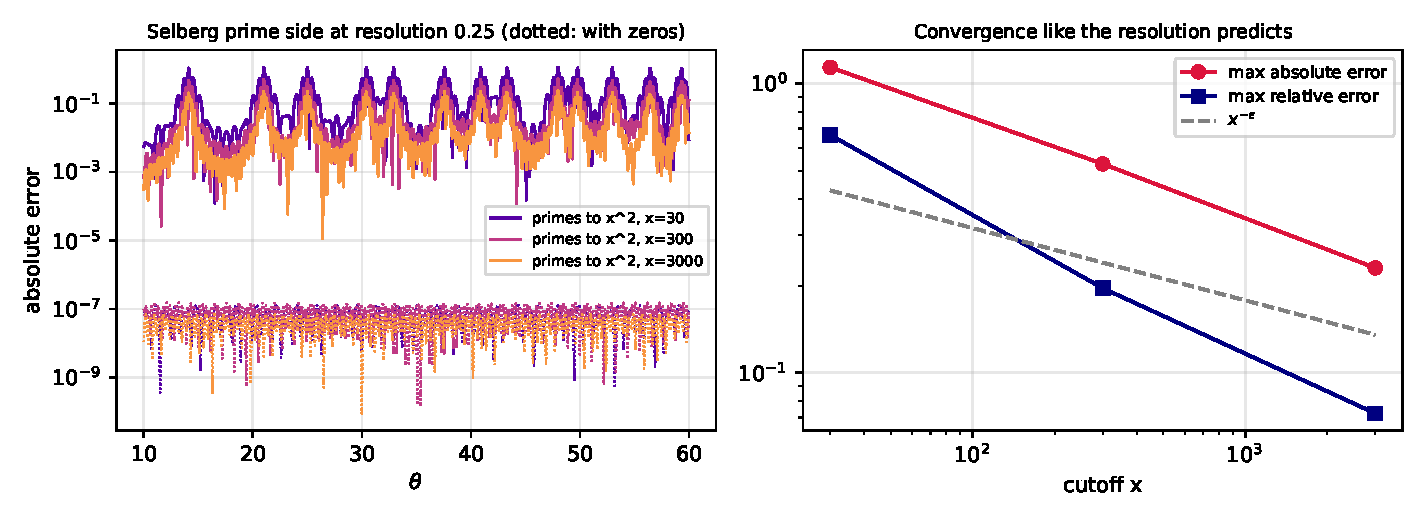
\includegraphics[width=\textwidth]{fig/selberg.pdf}
\caption{Left: absolute error of Selberg's smoothed prime side of $v_{3/4}$, at resolution $0.25$, for three cutoffs, and (dotted) with the sum over the first $1700$ zeros added. Right: the maximal absolute and relative errors against the cutoff, with $x^{-\varepsilon}$ for comparison.}
\label{fig:selberg}
\end{figure}

\subsection{Positivity: Brownian subordination and Weil's criterion}\label{sec:ch10:positivity}

The lemma cannot produce a Brownian first passage time to a random level from a positive input. Brownian motion with variance two per unit time first reaches a level $x>0$ at a time with Laplace transform $e^{-x\sqrt u}$, so its first passage time $T_Y$ to an independent level $Y\ge0$ has $\E e^{-uT_Y}=\E e^{-Y\sqrt u}$. The exponent $\log f(\alpha+s)/f(\alpha)=cs+\int(e^{-sx}+sx-1)L(dx)$ to which the lemma applies (Section~\ref{ch:clock}) would have to equal $-\log\E e^{-sY}$, which is concave in $s$ by H\"older's inequality, whereas $L\ge0$, $L\ne0$ makes it strictly convex, with second derivative $\int x^2e^{-sx}L(dx)>0$. With $c\ge0$ the lemma gives a GGC with Thorin density $(2\pi\sqrt z)^{-1}[c+\int2\sin^2(x\sqrt z/2)\,xL(dx)]$, but not a first passage time. Conversely, an infinitely divisible level with $\E e^{-sY}=\exp(-bs-\int(1-e^{-sx})\Pi(dx))$ enters the lemma with $c=b+\int x\,\Pi(dx)$ and the negative input $L=-\Pi$, and $T_Y$ receives the signed density $(2\pi\sqrt z)^{-1}[b+\int x\cos(x\sqrt z)\,\Pi(dx)]$. For a Poisson level ($\Pi=\delta_1$, $b=0$) this is $\cos(\sqrt z)/(2\pi\sqrt z)$, and $T_Y$ is not a GGC: it has an atom $e^{-1}$ at $0$. A positive input and a random level coexist only for pure drift, with transform $e^{-c\sqrt u}$ and Thorin density $c/(2\pi\sqrt z)$.

The reciprocal direction does work: for $Y\ge0$ infinitely divisible with finite mean $m$, $T_m\overset d=T_Y+R$, with $T_m$ the first passage time to the level $m$ and $R$ a GGC independent of $T_Y$, which for the clock is Proposition~\ref{tx:prop:W} and for a Barnes beta law is Proposition~\ref{tx3:prop:barnes}.

For $\xi$ there is no random level at any basepoint. By Stirling's formula and the polynomial growth of $\zeta$ in vertical strips, $|\xi(\alpha)/\xi(\alpha+it)|$ is at least $e^{\pi|t|/4}$ divided by a power of $|t|$, while $|\E e^{-itY}|\le1$; so $s\mapsto\xi(\alpha)/\xi(\alpha+s)$ is never a Laplace transform in $s$, although for $\alpha\ge1$ it is one in $u=s^2$ (Theorem~\ref{thm:poisson}). For $\alpha>1$ the input of $\xi$ is signed, and the positivity of $U_\alpha$ is created by the zeros through the Poisson kernels of Proposition~\ref{prop:struct}, not inherited from a positive input (Section~\ref{sec:ch6:consequences}); compare \cite[Remark 3.8]{P26}. At $\alpha=\tfrac12$ the obstruction is the drift zero case of Proposition~\ref{prop:nogo}, whose Brownian motion has variance one, and the curved boundaries of Section~\ref{ch:boundaries} take the place of the straight boundary with a random intercept. The obstruction concerns first passage alone (Section~\ref{ch:bphit}).

The same kernel puts Weil's criterion in variogram form. Section~\ref{ch:arith} defines the Thorin functional $U$ on the class $\mathcal T$ of functions $\varphi(z)=h(\sqrt z)$ with $h$ even, holomorphic on a strip $|\im r|\le\frac12+c$ for some $c>0$, and $O((1+|r|)^{-2-c})$ there. With $g(x)=\frac1{2\pi}\int h(r)e^{-irx}\,dr$,
\begin{equation}\label{eq:ch10:variogram}
\int_0^\infty\varphi(z)\,\frac{2\sin^2(x\sqrt z/2)}{2\pi\sqrt z}\,dz=g(0)-g(x),
\end{equation}
both sides being $\pi^{-1}\int_0^\infty h(r)(1-\cos xr)\,dr$. If $h\ge0$ on the real line, $g$ is positive definite and $g(0)-g(x)\ge0$ is a variogram. Weil's criterion \cite{Weil52} states that RH holds if and only if $\langle U,\varphi\rangle\ge0$ for every such $\varphi$, and by the explicit formula $U$ evaluates $\varphi$ at every zero. Formally, the lemma writes $\langle U,\varphi\rangle$ as the pairing of variograms with the canonical measure of \eqref{eq:split} taken at the centre, the measure $\nu$ of Section~\ref{ch:arith}, whose archimedean density and prime atoms are nonnegative and whose only negative input is the pole density $-e^{x/2}dx$. So RH says that on every variogram of a positive definite function the pole mass is dominated by the prime and archimedean mass. Both masses are infinite, and the absolutely convergent form of Section~\ref{ch:arith} makes the statement exact, the divergent constants cancelling through $\xi'(\tfrac12)=0$ (Section~\ref{sec:ch6:consequences}).

The linear programming formulation of \cite[Sections 18.2.8 and 18.2.9]{P26} works on this form, with the variograms as feasible directions. In a space of test functions of finite dimension the regularised domination is a feasibility problem with dual certificates, which Section~\ref{st:sec:wp5} proposes to solve at increasing dimension. Weil's criterion concerns $U$, which sees every zero, whereas the limit $\alpha\downarrow\tfrac12$ of the Thorin measures is $U_{\rm line}$, which pairs nonnegatively with every such $\varphi$ whatever the zeros do (Section~\ref{ch:arith}).

\section{Exercises}\label{chap:measure:ex}

\paragraph{On Section~\ref{ch:distances}.}
\begin{exercises}
\item Prove Proposition~\ref{prop:raw} for a positive measure $\nu$ on a general measurable space that does not charge the atoms of $U$.
\item Show that the total variation distance between the unit point masses at $a$ and $b$ is $2$ for $a\ne b$, and deduce that total variation cannot compare two atomic measures with slightly displaced atoms.
\item Compute the $L^1$ distance between the cumulative functions of a Cauchy kernel of width $\varepsilon$ and a unit step on $[-L,L]$, derive the $\varepsilon\log(1/\varepsilon)$ rate, and compare with the formula for a single step in Section~\ref{sec:ch9:mass}.
\item Derive the first order formula of Proposition~\ref{prop:mass} for the sinh clock of Section~\ref{ch:ggc}, where it reads $-(\varepsilon/\pi)f'/f$ with $f(\theta)=\sin(\pi\theta)/(\pi\theta)$, and compare it at $\Theta=m+\frac12$ with the exact mass $m+\pi^{-1}\arctan(\varepsilon/\Theta)$ of Section~\ref{sec:ch3:bench}; explain why the difference is of order $\varepsilon^3$.
\item Explain why the two point Richardson combination removes the linear term in $\varepsilon$ and the three point combination the quadratic term, and reproduce the heat trace errors $2.6\times10^{-7}$ and $1.7\times10^{-10}$ from the values of $W_\varepsilon(0.01)$ given in Section~\ref{sec:ch7:cumulative}.
\end{exercises}

\paragraph{On Section~\ref{ch:offline}.}
\begin{exercises}
\item Verify the expansion $\frac12(P_{\varepsilon+\delta}+P_{\varepsilon-\delta})-P_\varepsilon=\frac{\delta^2}2\partial_a^2P_a|_{a=\varepsilon}+O(\delta^4)$, show that the remainder has $L^1$ norm $O(\delta^4/\varepsilon^4)$, and compute the $L^1$ norm of $\partial_a^2P_a$ at $a=\varepsilon$.
\item Show that for $\delta>\varepsilon$ the kernel $P_{\varepsilon+\delta}-P_{\delta-\varepsilon}$ is negative exactly on $|x|<\sqrt{\delta^2-\varepsilon^2}$.
\item Compute the depth $2\varepsilon/(\pi(\delta^2-\varepsilon^2))$ of the negative dip of an off line pair at its centre, that is $\varepsilon/(\pi(\delta^2-\varepsilon^2))$ per displaced zero, compare it with the contribution $\varepsilon/(\pi(\varepsilon^2+\delta_j^2))\approx\varepsilon/(\pi\delta_j^2)$ of a line zero at distance $\delta_j$, and derive the local visibility condition of Section~\ref{ch:finite}.
\item Given the matched floor $\tilde d_{\rm match}(\varepsilon)$, derive the smallest displacement $\delta$ of a pair that keeps the count and would be detected, and evaluate it at $\varepsilon=0.05$ using Table~\ref{tab:tv}.
\end{exercises}

\paragraph{On Section~\ref{ch:turing}.}
\begin{exercises}
\item Show that $I(\varepsilon)=\int_0^T\log|\xi(\frac12+\varepsilon+it)|\,dt$ is continuous for $\varepsilon\ge0$, that its derivative jumps by $2\pi$ when the line $\re s=\frac12+\varepsilon$ crosses a zero, and deduce the second identity of Proposition~\ref{prop:littlewood}.
\item Prove Proposition~\ref{prop:zerodensity} in detail, paying attention to the orientation of each side of the rectangle.
\item\label{ex:ch9:pair} Show that the kernels $P_{\varepsilon+\delta}$ and $-P_{\delta-\varepsilon}$ of an off line pair at distance $\delta>\varepsilon$ from the line have total mass zero, and compute to leading order the mass that they and their mirror images at $-\gamma$ put on a window $(0,T]$ containing the ordinate $\gamma$. Explain how the factor two in Proposition~\ref{prop:zerodensity} accounts for the pair.
\item Using the first order formula for $\tau_\varepsilon(T)$ in Section~\ref{sec:ch9:count}, predict $\tau_{0.05}(200)$ from $\Xi'(200)/\Xi(200)=-1.2506879$ and compare with Table~\ref{tab:zerodensity}; estimate the coefficient of the $\varepsilon^3$ term from the rows $\varepsilon=0.01$ and $0.02$.
\item\label{ex:ch9:littlewood} Show that Littlewood's lemma follows from Proposition~\ref{prop:littlewood} and Proposition~\ref{prop:zerodensity} by integrating in $\varepsilon$.
\end{exercises}

\paragraph{On Section~\ref{ch:sin2more}.}
\begin{exercises}
\item Show that $\frac1\pi\int_0^\Theta(1-\cos\theta x)\,d\theta=\frac1\pi(\Theta-\sin(\Theta x)/x)$ and, for $\alpha>1$, derive the Dirichlet series for $\arg\zeta(\alpha+i\Theta)$ from the integrated sine squared lemma.
\item Implement Selberg's formula at $s=\frac34+i\theta$ with $x=100$ and check that adding the zero sum over the first hundred zeros reduces the error to the size of the omitted zeros.
\item Estimate, from the single zero law, the cutoff $x$ needed for six correct digits of $v_{0.55}(\theta)$ at an ordinate $\theta=\gamma$ from the primes, and compare with the cost of the P\'olya route at the same point.
\item Show that $g(0)-g(x)\ge0$ for every real positive definite function $g$, and that $g(0)-g(x)$ is conditionally negative definite.
\end{exercises}

\chapter{Weak limits, hyperbolic complete monotonicity and a Bosch type theorem}\label{chap:hcm}\chaptermark{Weak limits, HCM and a Bosch type theorem}

Sections~\ref{ch:boschA} and \ref{ch:boschB} bring in Bosch's theorem on powers of the half Cauchy law. The first explains why his result cannot be transferred as an input, and the second transfers his method instead and proves a threshold theorem for powers of the reciprocal Xi function, in which the angle of the zeros replaces Bosch's drift parameter and RH is the extreme case.

\section{The limit of vanishing resolution}\label{ch:weak}

Neither closure under weak limits nor Bondesson's theorem reaches RH.

\subsection{Weak limits of Thorin measures}\label{sec:weak:limits}

\begin{theorem}[Thorin \cite{Thorin77a,Thorin}; Bondesson {\cite[Theorem 3.1.5]{Bondesson}}; see also {\cite[Theorem 18.9]{P26}}]
The class of GGC laws is closed under convergence in law.
\end{theorem}



\begin{corollary}\label{cor:weak:closure}
RH holds if and only if there are GGC variables $X_N$ with $\E e^{-uX_N}\to1/G(u)$ for all $u$ in a set with an accumulation point in $(0,\infty)$ \cite[Propositions 18.10 and 18.14]{P26}.
\end{corollary}

\begin{proof}
The transforms are analytic and bounded by one on $\re u>0$, so by Vitali's theorem they converge locally uniformly there, and the limit is $1/G$ on $(0,\infty)$. Since $1/G(u)\to1$ as $u\downarrow0$, the $X_N$ converge in law to a proper limit with transform $1/G$, which is a GGC by the closure theorem, and Proposition~\ref{prop:rigid} gives RH. Conversely, under RH the clock variable $T$ is a GGC with transform $1/G$; take $X_N=T$.
\end{proof}

The Cauchy flow $\varepsilon\mapsto\rho_\varepsilon$ of Section~\ref{ch:clock} is the candidate at hand. Its measures $\mu_\varepsilon$ are the Thorin measures of $\xi(\alpha)/\xi(\alpha+\sqrt u)$ at $\alpha=\tfrac12+\varepsilon$ whenever these are GGC transforms (Theorem~\ref{thm:poisson}), the transforms converge to $1/G$ pointwise as $\varepsilon\downarrow0$, and the measures converge vaguely. The flow fails for two reasons.

First, the limit is the wrong measure. As shown after Proposition~\ref{prop:struct}, $\mu_\varepsilon\to U_{\rm line}$ vaguely whatever the truth of RH \cite[Proposition 9.5]{P17}, because the contribution of an off line pair tends to zero in total variation (Proposition~\ref{prop:signature}(ii)); the limit omits the off line zeros. It is the Thorin measure of the clock only under RH, since the Thorin functional $U$ of Section~\ref{ch:arith} counts every zero and $U=U_{\rm line}$ exactly when RH holds (Section~\ref{sec:ch14:functional} and \cite[Proposition 7.6]{P26}). Positivity of the vague limit therefore carries no information.

Second, the closure theorem needs GGC laws along the sequence. The flow supplies a law at every resolution with no hypothesis, that of the shifted clock $T_\alpha$ of Theorem~\ref{bp:thm:alpha} at $\alpha=\tfrac12+\varepsilon$, but at small $\varepsilon$ it supplies a GGC law only under the hypothesis to be proved: the transform at basepoint $\tfrac12+\varepsilon$ is a GGC transform if and only if no zero lies to the right of the line $\re s=\tfrac12+\varepsilon$ (Theorem~\ref{thm:poisson}). Positivity of $\rho_\varepsilon$ at that one $\varepsilon$ is necessary for this but is not known to imply it, since near a cluster of line zeros the negative kernel of an off line pair can be outweighed by the kernels of its neighbours (Exercise~\ref{ex:ch2:line} and Section~\ref{sec:ch13:visibility}). Positivity of $\rho_{\varepsilon'}$ for every $\varepsilon'>\varepsilon$ does imply it, as shown in Remark~\ref{rem:ch2:oneline}; for $\varepsilon=0$ this is Lagarias's criterion \cite{Lagarias}, which is RH. Weak closure adds the endpoint $\varepsilon=0$ to a family already known to consist of GGCs; it cannot show that the family consists of GGCs \cite[Remark 3.10]{P26}.

On the window $0\le\theta\le200$ the P\'olya route computes $\min\rho_\varepsilon=0.0147\,\varepsilon>0$ at each of the eight resolutions of Table~\ref{tab:tv}, down to $\varepsilon=0.005$ (Section~\ref{sec:ch6:measure}); with the verification of RH to height $3\times10^{12}$ this is a theorem, since for every $\varepsilon\le6.85$ the minimum of $\rho_\varepsilon$ over $[0,3\times10^{12}-1.21]$ is $\rho_\varepsilon(0)$ (Theorem~\ref{thm:dbeta:minall} and Remark~\ref{rem:dbeta:margin}), and Section~\ref{st:sec:wp2} lists what would make the P\'olya computation itself a certificate.

Weak convergence becomes useful only with approximants whose positivity is proved independently of $\xi$, such as Beurling generalised prime systems whose zeta functions provably have only real ordinates, finite Krein strings, and the partial products over verified zeros completed by the Weyl tail; the last two are the Kent approximants of Section~\ref{sec:ch18:kent}, without and with the Weyl tail. For such approximants the distances of Section~\ref{ch:distances} are the right measure of the approximation. Verification also removes factors from the question: if the first $N$ zeros are verified to lie on the line, then $1/G_N$, with $G_N(u)=\prod_{k\le N}(1+u/\gamma_k^2)$, is a GGC transform with no hypothesis, and RH holds if and only if the tail factor $G_N/G$ is a GGC transform as well \cite[Corollary 18.11]{P26}.


\subsection{The HCM form of the Thorin condition}\label{sec:weak:hcm}

Bondesson's theorem (Section~\ref{sec:ch3:hierarchy}; \cite[Theorem 6.1.1]{Bondesson}, see also \cite{JRY}) and the results of Section~\ref{ch:clock} give the following.

\begin{corollary}\label{cor:hcm}
(i) For every $\alpha\ge1$ the function $\varphi_\alpha(u)=\xi(\alpha)/\xi(\alpha+\sqrt u)$ is HCM, unconditionally. (ii) The reciprocal Xi function $\varphi_{1/2}(u)=\xi(\tfrac12)/\xi(\tfrac12+\sqrt u)$, which is the clock $1/G$, is HCM if and only if RH holds.
\end{corollary}

\begin{proof}
(i) is Theorem~\ref{thm:poisson} with Bondesson's theorem, and (ii) is Proposition~\ref{prop:rigid} with Bondesson's theorem.
\end{proof}



By the Hadamard product \eqref{eq:ch2:hadamard}, with $a_k=-(\rho_k-\tfrac12)^2$ and $w=v+1/v$,
\begin{equation}\label{eq:hcmprod}
\varphi_{1/2}(uv)\,\varphi_{1/2}(u/v)=\prod_k\frac{a_k^2}{a_k^2+a_k\,u\,w+u^2}=\prod_k\frac{a_k/u}{w+c_k(u)},\qquad c_k(u)=\frac{a_k}{u}+\frac{u}{a_k}.
\end{equation}
The numbers $c_k(u)$ are local to this subsection, and are not the derivatives $c_k(t)$ of the heat trace in Section~\ref{ch:heat}. An off line pair, with values $a$ and $\bar a$ of $a_k$, contributes $(|a|^2/u^2)/((w+c)(w+\bar c))$ with $c=c(u)$ complex, and $1/((w+c)(w+\bar c))$ is the Laplace transform of the signed function $e^{-t\re c}\sin(t\im c)/\im c$. At a single $u$ the remaining factors may smooth this to a positive function; failure is guaranteed only across all $u$, by Bondesson's theorem. At $u=|a|$ both values of $c$ equal $2\cos\arg a$, and the pair contributes $(w+2\cos\arg a)^{-2}$, which is completely monotone on $[2,\infty)$. Complete monotonicity in $w$ at finitely many $u$ is therefore necessary for HCM but not sufficient.

We test this necessary condition. From $60$ digit values of $\xi$ at real arguments, computed by \eqref{eq:xi} without cancellation, numerical differentiation gives the normalised derivatives $d_k=(-1)^k\partial_w^kH_u(w)/H_u(w)$ of $H_u(w)=\varphi_\alpha(uv)\,\varphi_\alpha(u/v)$ for $k\le6$, $u\in\{1,25,400\}$ and $w\in\{2.05,3,5,10,20,50\}$, at $\alpha=\tfrac12$ and at the control $\alpha=1$. All $216$ values are positive (Figure~\ref{fig:hcm} shows $w=3$ and $w=20$), and the signs are certified: from the Taylor coefficients of $H_u$ in $w$, computed in ball arithmetic \cite{Arb} from $\xi(s)=\frac12s(s-1)\pi^{-s/2}\Gamma(\frac s2)\zeta(s)$, and so independently of the P\'olya route, every $d_k$ is enclosed in a ball of relative radius below $10^{-70}$ that lies in $(0,\infty)$. Under RH, \eqref{eq:hcmprod} gives $H_u(w+t)/H_u(w)=\E e^{-tY}$ with $Y=\sum_ke_k/(w+c_k(u))$ and independent standard exponentials $e_k$, so $d_k=\E Y^k$ is of order $d_1^k$. The smallest value, $2.5\times10^{-10}$ at $\alpha=\tfrac12$, $u=1$, $w=50$, $k=6$, is $2.54\,d_1^6$ with $d_1=0.0215$: it reflects the scale of $Y$, to which many zeros contribute, not closeness to a sign change. The test is consistent with (ii) and cannot decide it (Section~\ref{ch:finite}, Table~\ref{tab:ch13:see}, and \cite[Chapter 11]{P26}).

Under RH the clock variable is $T=\sum_{\gamma>0}e_\gamma/\gamma^2$ (Proposition~\ref{prop:rigid}), and if moreover the zeros are simple and satisfy two further hypotheses, its density is not HCM (Theorem~\ref{bs:thm:nb}); for the Cauchy analogue of the clock variable this holds unconditionally (Theorem~\ref{bs:thm:eta}).

\begin{figure}[t]
\centering
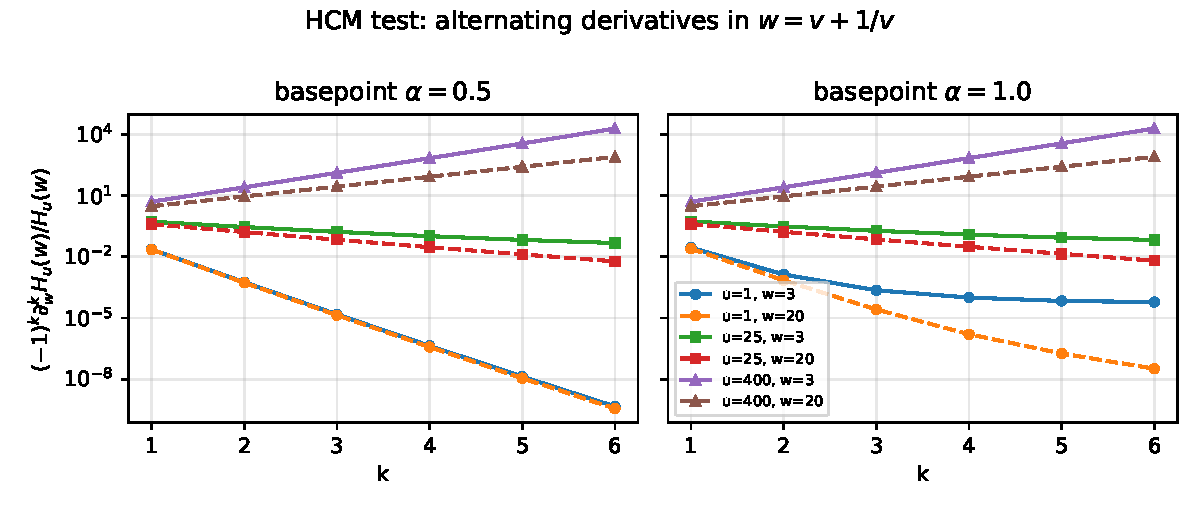
\includegraphics[width=0.95\textwidth]{fig/hcm.pdf}
\caption{Normalised alternating derivatives $(-1)^k\partial_w^kH_u(w)/H_u(w)$ of $H_u(w)=\varphi_\alpha(uv)\varphi_\alpha(u/v)$ for $1\le k\le6$, $u\in\{1,25,400\}$ and $w\in\{3,20\}$, computed from the P\'olya density, at the centre $\alpha=\tfrac12$ and at the unconditional basepoint $\alpha=1$. }
\label{fig:hcm}
\end{figure}

\section{Bosch's half Cauchy theorem and HCM of the reciprocal Xi function}\label{ch:boschA}

By Corollary~\ref{cor:hcm}(ii) of Section~\ref{ch:weak} the clock $\varphi=1/G$ is HCM if and only if RH holds; this is the HCM form of the reciprocal Xi programme of \cite{P17}. In this section and in Section~\ref{ch:boschB} the clock is a function of $s$, the variable $u$ of Section~\ref{ch:clock}: $\varphi(s)=\xi(\frac12)/\xi(\frac12+\sqrt s)$ is the function $\varphi_{1/2}$ of Corollary~\ref{cor:hcm}. A sharp HCM theorem for a nearby, exactly solvable function might transfer to $\varphi$, and the candidate is Bosch's theorem on powers of the half Cauchy law \cite{boBosch}.

\subsection{HCM and Bosch's theorem at the half Cauchy point}\label{bh:sec:bosch}

Bosch's theorem concerns densities, so we recall HCM from Section~\ref{sec:ch3:hierarchy} in the form that applies to them: a continuous function $f:(0,\infty)\to[0,\infty)$ is HCM if for every $u>0$ the map $v\mapsto f(uv)f(u/v)$, the pair function of $f$ at $u$, is a completely monotone function of $w=v+v^{-1}$ on $[2,\infty)$, and a positive random variable is HCM if it has an HCM density. In logarithmic coordinates $u=e^a$, $v=e^y$ the condition reads: $y\mapsto f(e^{a+y})f(e^{a-y})$ is completely monotone in $w=2\cosh y$. We use the following facts, all due to Bondesson; (F1), (F2), (F5) and (F6) are also stated in Section~\ref{sec:ch3:hierarchy}.

\begin{enumerate}
\item[(F1)] If $X_1,X_2$ are independent and HCM then $X_1X_2$ and $X_1/X_2$ are HCM \cite[Theorem 5.1.1]{Bondesson}.
\item[(F2)] If $X$ is HCM then $X^q$ is HCM for $|q|\ge 1$ \cite[pp.~68 and 69]{Bondesson}. The mechanism is that for $|p|\le 1$ the function $v^p+v^{-p}$ is a Bernstein function of $v+v^{-1}$, so if $h$ is an HCM function then so is $x\mapsto h(x^p)$ for $|p|\le 1$; if $X$ has density $f$, the density of $X^q$ is $|q|^{-1}x^{1/q-1}f(x^{1/q})$, and the power factor is HCM by (F3).
\item[(F3)] Pointwise products of HCM functions are HCM, and powers $x^{r}$, $r\in\R$, are HCM \cite[p.~68]{Bondesson}.
\item[(F4)] Pointwise limits of HCM functions, when finite and positive, are HCM \cite[p.~68 and Theorem 5.1.3]{Bondesson}.
\item[(F5)] Every HCM law is a GGC \cite[Theorem 5.1.2]{Bondesson}.
\item[(F6)] A probability law on $[0,\infty)$ is GGC if and only if its Laplace transform is an HCM function \cite[Theorem 6.1.1]{Bondesson}.
\item[(F7)] A function $f$ that is not identically zero is HCM if and only if
\begin{equation}\label{bs:eq:bond}
\begin{aligned}
f(x)&=Kx^{r-1}h_1(x)h_2(1/x),\\
h_j(x)&=\exp\Bigl(-b_jx+\int_{(0,\infty)}\log\frac{1+t}{x+t}\,\Gamma_j(dt)\Bigr),
\end{aligned}
\end{equation}
with $K>0$, $r\in\R$, $b_j\ge0$ and nonnegative measures $\Gamma_j$ satisfying $\int(1+t)^{-1}\Gamma_j(dt)<\infty$ \cite[(5.2.3) and Theorem 5.3.1]{Bondesson}. In particular every HCM function that is not identically zero extends to an analytic and zero free function on $\C\setminus(-\infty,0]$ \cite[p.~68]{Bondesson}.
\end{enumerate}

\begin{theorem}[Bosch {\cite[Theorem 1.2]{boBosch}}]
Let $T_\alpha=(Z_\alpha/\tilde Z_\alpha)^\alpha$ with $Z_\alpha,\tilde Z_\alpha$ independent positive $\alpha$ stable (here $\alpha$ is a stability index, not a basepoint, and $T_\alpha$ is not the variable of Theorem~\ref{thm:poisson}). Then $T_\alpha$ has density $\sin(\pi\alpha)/(\pi\alpha(t^2+2t\cos\pi\alpha+1))$, a half Cauchy law with drift, and the density of $T_\alpha^\beta$ is HCM if and only if $\alpha\le1/2$ and $|\beta|\ge 1/(1-\alpha)$.
\end{theorem}

At $\alpha=1/2$ we have $T_{1/2}\stackrel{d}{=}|C|$ with density $2/(\pi(1+t^2))$. The density of $|C|^\beta$ is
\[
f_\beta(x)=\frac{2}{\pi|\beta|}\,\frac{x^{1/\beta-1}}{1+x^{2/\beta}},\qquad x>0 .
\]
With $x=e^{a\pm y}$ and $q=2/|\beta|$ a short computation gives
\begin{equation}\label{bh:eq:pair}
f_\beta(e^{a+y})f_\beta(e^{a-y})=\frac{4}{\pi^2\beta^2}\,e^{-2a}\,\frac{1}{2\cosh(qa)+2\cosh(qy)} .
\end{equation}
So at $\alpha=1/2$ Bosch's theorem is the statement that $1/(c+\cosh(qy))$ is completely monotone in $\cosh y$ for every $c\ge1$ exactly when $q\le 1$; here $c=\cosh(qa)$, which ranges over $[1,\infty)$.

\begin{proposition}\label{bh:prop:notHCM}
The half Cauchy density is not HCM.
\end{proposition}

\begin{proof}
Take $\beta=1$, so $q=2$ in \eqref{bh:eq:pair}. Since $\cosh(2a)+\cosh(2y)=2\sinh^2a+w^2/2$ with $w=2\cosh y$, the pair function is proportional to $h(w)=1/(c^2+w^2)$ with $c=2|\sinh a|>0$ for $a\ne0$. For $x>0$,
\[
h(2+x)=\int_0^\infty e^{-xt}\,e^{-2t}\,\frac{\sin(ct)}{c}\,dt .
\]
If $h$ were completely monotone on $(2,\infty)$, Bernstein's theorem would give $h(2+x)=\int e^{-xt}\mu(dt)$ with $\mu\ge0$, and uniqueness of the Laplace transform would force $\mu(dt)=e^{-2t}c^{-1}\sin(ct)\,dt$, which is not nonnegative.
\end{proof}

\begin{proposition}\label{bh:prop:square}
The density of $|C|^\beta$ is HCM for $|\beta|\ge2$.
\end{proposition}

\begin{proof}
For $q=2/|\beta|\le1$ the function $\cosh(qy)$ is a Bernstein function of $\cosh y$ by (F2), and $x\mapsto 1/(c+x)$ is completely monotone for $c>0$, so the composition in \eqref{bh:eq:pair} is completely monotone.
\end{proof}

At $\alpha=1/2$ sufficiency is therefore elementary; the deep part of Bosch's paper is $\alpha<1/2$.

\subsection{The half Cauchy law and the Riemann Xi function}\label{bh:sec:dict}

On the Cauchy side everything is explicit. The logarithm of $|C|$ has density $g_C(y)=1/(\pi\cosh y)$ and characteristic function $\sech(\pi t/2)$. The Weierstrass product
\[
\sech\Bigl(\frac{\pi t}{2}\Bigr)=\prod_{k\ge1}\Bigl(1+\frac{t^2}{(2k-1)^2}\Bigr)^{-1}
\]
says $\log|C|\stackrel{d}{=}\sum_{k\ge1}L_k/(2k-1)$ with $L_k$ independent standard Laplace variables. The Mellin transform is $\E|C|^z=\sec(\pi z/2)$ for $|\Re z|<1$, the reciprocal of $\cos(\pi z/2)$, a function of the Laguerre P\'olya class with real zeros $\pm(2k-1)$; these odd integers are the frequencies of the half Cauchy law. The Cauchy reciprocal Xi function
\[
\varphi_C(s)=\E|C|^{i\sqrt{s}}=\sech\Bigl(\frac{\pi\sqrt{s}}{2}\Bigr)=\prod_{k\ge1}\Bigl(1+\frac{s}{(2k-1)^2}\Bigr)^{-1}
\]
is the Laplace transform of the GGC $\sum_ke_k/(2k-1)^2$, with independent standard exponentials $e_k$ and Thorin measure $\sum_k\delta_{(2k-1)^2}$, hence HCM by (F6). The checks below that name no source used mpmath \cite{mpmath} at 20 to 30 digits. Bourgade, Fujita and Yor \cite{boBFY} derive Euler's formulae for $\zeta(2n)$ from products of independent Cauchy variables, whose Mellin transforms are powers of $\sec(\pi z/2)$. Section~\ref{ch:riesz} develops their construction.

On the Riemann side the frequencies are the zeros $\gamma$ of $\Xi(z)=\xi(\frac12+iz)$. By \eqref{eq:ch2:hadamard}, whose product converges absolutely because $\sum|\gamma|^{-2}<\infty$, unconditionally
\[
\Xi(z)=\Xi(0)\prod_{\gamma}\Bigl(1-\frac{z^2}{\gamma^2}\Bigr),
\]
the product over zeros $\gamma$ of $\Xi$ with $\Re\gamma>0$, counted with multiplicity. No zero is purely imaginary because $\xi(\sigma)>0$ for real $\sigma$. Hence the clock is
\[
\varphi(s)=\frac{\Xi(0)}{\Xi(i\sqrt{s})}=\frac{\xi(1/2)}{\xi(1/2+\sqrt{s})}=\prod_\gamma\Bigl(1+\frac{s}{\gamma^2}\Bigr)^{-1}.
\]
Under RH define, in the spirit of Biane, Pitman and Yor \cite{BPY01}, $\log W=\sum_\gamma L_\gamma/\gamma$ with independent standard Laplace variables $L_\gamma$. Then $\E W^z=\Xi(0)/\Xi(z)$ for $|\Re z|<\gamma_1\approx14.1347$, the characteristic function of $\log W$ is $\xi(1/2)/\xi(1/2+t)$, and $\varphi(s)=\E W^{i\sqrt{s}}$. The variable $W$, not to be confused with the heat trace $W(t)$, exists without RH: $\log W$ has the law of the variable $Z\sqrt{2T}$ of the van Dantzig pair of Section~\ref{ch:clock}, where $Z$ is standard normal and independent of the clock variable $T$. Only the series for $\log W$ needs RH. Biane, Pitman and Yor represent $2\xi$ itself, not its reciprocal, as a Mellin transform (Sections~\ref{ch:clock} and \ref{ch:basepoint}).

\begin{table}[h]
\centering\small
\begin{tabular}{@{}lll@{}}
\toprule
 & half Cauchy & Riemann\\
\midrule
entire function & $\cos(\pi z/2)$ & $\Xi(z)/\Xi(0)$\\
frequencies & $2k-1$ & $\gamma$\\
log variable & $\sum_k L_k/(2k-1)$ & $\sum_\gamma L_\gamma/\gamma$\\
Mellin transform & $\sec(\pi z/2)$ & $\Xi(0)/\Xi(z)$\\
reciprocal Xi & $\sech(\pi\sqrt{s}/2)$ & $\xi(1/2)/\xi(1/2+\sqrt{s})$\\
Thorin measure & $\sum_k\delta_{(2k-1)^2}$ & $\sum_\gamma\delta_{\gamma^2}$\\
exit time & Brownian motion on $(-1,1)$ & Krein string with spectrum $\{\gamma^2\}$\\
density of the power & HCM iff $|\beta|\ge2$ (Bosch) & HCM only if $|\beta|\ge\gamma_2-\gamma_1$\\
\bottomrule
\end{tabular}
\caption{The dictionary. In the Riemann column the Mellin transform (Section~\ref{ch:clock} and Theorem~\ref{bs:thm:gpos}) and the reciprocal Xi function are unconditional, the log variable and the Thorin measure presume RH, and the exit time, the hitting time of Kent's theorem (Section~\ref{sec:ch18:kent}), presumes RH and simple zeros. The last entry is the necessary condition of Theorem~\ref{bs:thm:gap}, which assumes RH, simple zeros and a growth condition on $1/|\zeta'(\rho)|$; sufficiency is open (Question~\ref{bs:q:gap}).}
\label{bh:tab:dict}
\end{table}

On the Riemann side the analogue of $g_C$ is the density of $\log W$. The function $t\mapsto\xi(1/2)/\xi(1/2+t)$ is defined for all real $t$ without any hypothesis ($\xi$ has no real zeros) and decays like $\exp(-\tfrac12|t|\log|t|)$, so its Fourier inverse
\[
g(y)=\frac1\pi\int_0^\infty\frac{\xi(1/2)}{\xi(1/2+t)}\cos(ty)\,dt
\]
is an even function with $\int g=1$, entire because the integrand decays faster than any exponential; $g>0$ unconditionally (Theorem~\ref{bs:thm:gpos}). Under RH, with simple zeros and $\log(1/|\zeta'(\rho_n)|)=O(\gamma_n)$, the residues at the poles $\pm i\gamma_n$ of the integrand give, for $|y|>u_0$ with the constant $u_0\ge\pi/4$ of Theorem~\ref{bs:thm:gap},
\begin{equation}\label{bh:eq:laplace}
g(y)=\sum_n\frac{\gamma_n}{2}A_ne^{-\gamma_n|y|},\qquad A_n=\prod_{m\ne n}\Bigl(1-\frac{\gamma_n^2}{\gamma_m^2}\Bigr)^{-1},
\end{equation}
the analogue of $g_C(y)=(2/\pi)\sum_k(-1)^{k-1}e^{-(2k-1)|y|}$, which converges for every $y\ne0$ because its coefficients are bounded. The Riemann coefficients $A_1\approx50.9$, $A_2\approx-2664.6$, $A_3\approx31420$ (\texttt{code/\allowbreak README.md}) alternate in sign, as the Cauchy coefficients do, but grow roughly like $e^{\pi\gamma_n/4}$ (Theorem~\ref{bs:thm:gap}), so \eqref{bh:eq:laplace} diverges for $|y|<\pi/4$.

\subsection{The reciprocal Xi function is HCM if and only if RH holds}\label{bh:sec:main}

Bosch's method works with the singularities of a function and with its logarithmic derivative, so we state Corollary~\ref{cor:hcm}(ii) in four forms. Form (iii) is Proposition~\ref{prop:rigid}, and since $\psi=G'/G$, form (iv) is the Stieltjes form of the Thorin condition in Section~\ref{ch:intro}. A Stieltjes function is a function $a/s+b+\int_{(0,\infty)}\sigma(dt)/(s+t)$ with $a,b\ge0$ and $\sigma$ a nonnegative measure satisfying $\int(1+t)^{-1}\sigma(dt)<\infty$ \cite[Definition 2.1]{boSSV}.

\begin{theorem}\label{bh:thm:main}
The following are equivalent.
\begin{enumerate}
\item[(i)] The Riemann Hypothesis.
\item[(ii)] $\varphi(s)=\xi(1/2)/\xi(1/2+\sqrt{s})$ is HCM on $(0,\infty)$.
\item[(iii)] $\varphi$ is the Laplace transform of a GGC, namely $\sum_\gamma e_\gamma/\gamma^2$.
\item[(iv)] $\psi(s)=-\varphi'(s)/\varphi(s)=\dfrac{1}{2\sqrt{s}}\dfrac{\xi'}{\xi}\bigl(\tfrac12+\sqrt{s}\bigr)$ is a Stieltjes function.
\end{enumerate}
\end{theorem}

\begin{proof}
(i) implies (iii): each factor $(1+s/\gamma^2)^{-1}$ is the Laplace transform of an exponential variable with rate $\gamma^2>0$, and the product converges because $\sum\gamma^{-2}<\infty$; the sum $\sum_\gamma e_\gamma/\gamma^2$ converges almost surely. (iii) implies (ii) by (F6).

(ii) implies (i): by (F7), $\varphi$ extends analytically to $\C\setminus(-\infty,0]$. Suppose a zero $\gamma$ has $\Im\gamma\ne0$. Since $\Re\gamma>0$ the point $s_0=-\gamma^2$ has $\Im s_0=-2\Re\gamma\,\Im\gamma\ne0$, and its principal square root is $\pm i\gamma$, so $\xi(1/2+\sqrt{s_0})=\Xi(\pm\gamma)=0$ by evenness. Then $\varphi$ has a pole at a nonreal point of $\C\setminus(-\infty,0]$, a contradiction.

(i) is equivalent to (iv): under RH, $\psi(s)=\sum_\gamma 1/(s+\gamma^2)$, a Stieltjes function with measure $\sum_\gamma\delta_{\gamma^2}$. Conversely a Stieltjes function is analytic on $\C\setminus(-\infty,0]$, and an off line zero produces the nonreal pole $s_0$ of $\psi$ found above.
\end{proof}

Condition (iv) is a companion of Lagarias's criterion \cite{Lagarias}, and it is the pole test of Table~\ref{tab:ch3:diag} in analytic form.

The de Bruijn Newman flow embeds $\varphi$ in a family of the same kind. Let $\Phi_{\rm dBN}$ and $H_t(z)=\int_0^\infty e^{tu^2}\Phi_{\rm dBN}(u)\cos(zu)\,du$ be as in Section~\ref{ch:dbn}, so that $H_0(z)=\frac18\Xi(z/2)$. Put $\varphi_t(s)=H_t(0)/H_t(2i\sqrt{s})$, the function $R_t$ of Theorem~\ref{rz:thm:dbn}, so that $\varphi_0=\varphi$. The function $H_t$ is even, real on $\R$ and entire of order one, as in the proof of Theorem~\ref{rz:thm:dbn}, so its Hadamard product in $z^2$ converges. It is positive on the imaginary axis, $H_t(iy)=\int_0^\infty e^{tu^2}\Phi_{\rm dBN}(u)\cosh(yu)\,du>0$, since $\Phi_{\rm dBN}(u)=\frac12\Phi(2u)>0$; hence $\varphi_t>0$ on $(0,\infty)$ and no zero of $H_t$ is purely imaginary. With these facts the argument of Theorem~\ref{bh:thm:main} applies verbatim.

\begin{corollary}\label{bh:cor:dbn}
$\varphi_t$ is HCM if and only if $t\ge\Lambda$, the de Bruijn Newman constant. Hence $\varphi_t$ is HCM for $t\ge0.22$ \cite{Polymath}, $\varphi_t$ is not HCM for $t<0$ \cite{RodgersTao}, and RH holds if and only if $\varphi_t$ is HCM for every $t>0$.
\end{corollary}

\begin{proof}
The zeros of $H_t$ are real if and only if $t\ge\Lambda$ (de Bruijn \cite{deBruijn}, Newman \cite{Newman1976}). If RH holds, $H_0$ has only real zeros, so $\Lambda\le0$ and $\varphi_t$ is HCM for every $t>0$. Conversely, $\varphi_t\to\varphi_0$ pointwise as $t\downarrow0$, so if every $\varphi_t$ with $t>0$ is HCM then $\varphi$ is HCM by (F4), and Theorem~\ref{bh:thm:main} gives RH.
\end{proof}

The bound $\Lambda\le0.2$ of Platt and Trudgian \cite{PT21} (Section~\ref{ch:dbn}) lowers the unconditional threshold from $0.22$ to $0.2$. The reciprocal Xi function, if HCM at all, is HCM with no room to spare, since the property fails for every $t<0$. This is the Riemann counterpart of the boundary $|\beta|=1/(1-\alpha)$ in Bosch's theorem, which is attained; the difference is that Bosch can compute on the boundary because his kernel is explicit.

\subsection{What Bosch's theorem can and cannot supply}\label{bh:sec:use}

Bosch's theorem cannot be the input to a proof of Theorem~\ref{bh:thm:main}. For products the reason is elementary.

\begin{proposition}\label{bh:prop:closure}
For any positive numbers $c_n$ with $\sum_n c_n^{-1}<\infty$ the function $\prod_n(1+s/c_n)^{-1}$ is HCM. If one $c_n$ is replaced by a pair $c,\bar c$ with $c$ nonreal, the product is still positive on $(0,\infty)$ but is not HCM.
\end{proposition}

\begin{proof}
The first claim is the argument for (i) implies (ii) in Theorem~\ref{bh:thm:main}. For the second, $(1+s/c)(1+s/\bar c)=|1+s/c|^2>0$ for real $s$, and the product has a pole at the nonreal point $-c$, contradicting (F7).
\end{proof}

Heuristically, every HCM closure operation carries real frequencies to real frequencies and none creates them: on Mellin transforms, products and quotients of independent variables multiply the transforms, and powers rescale the frequencies. Bosch's theorem lives in the class where the frequency set $\{2k-1\}$ is given, so any deduction of Theorem~\ref{bh:thm:main} from it must import the location of the $\gamma$ from elsewhere.

Nor can the Riemann statement be proved factor by factor. Write $\xi(1/2+\sqrt{s})=\tfrac12(s-\tfrac14)\,\pi^{-(1/2+\sqrt s)/2}\,\Gamma(\tfrac14+\tfrac{\sqrt s}{2})\,\zeta(\tfrac12+\sqrt s)$. The reciprocal factors are not individually HCM. The reciprocal of $\pi^{-(1/2+\sqrt s)/2}$ is $\pi^{1/4}\pi^{\sqrt s/2}$, and the pair function of $\pi^{\sqrt s/2}$ is $\exp(\tfrac12\log\pi\,\sqrt u\,\sqrt{w+2})$, which increases in $w$. The factor $1/\zeta(1/2+\sqrt s)$ changes sign at $s=1/4$, since $\zeta<0$ on $(1/2,1)$, and HCM functions are positive. The positive combination $1/((s-\tfrac14)\zeta(\tfrac12+\sqrt s))$ is continuous at $s=1/4$, and by the argument of Theorem~\ref{bh:thm:main} any HCM statement for it would again imply RH. It is the function to which the $\sech$ expansion of $1/\zeta(\tfrac12+\sqrt s)$ in Theorem~\ref{rz:thm:sech} should be applied.

Bosch's theorem is a density statement, and HCM of a density differs from HCM of a Laplace transform: the density of $|C|$ is not HCM, yet $\varphi_C$ is. On the Cauchy side the two levels are linked only because $\sech$ is self dual, its own Fourier transform up to scaling, so that the density $g_C$ of $\log|C|$ and the transform $\varphi_C$ are the same function in different coordinates. On the Riemann side there is no self duality: the density level object is $g$ in \eqref{bh:eq:laplace}, the Fourier inverse of $\Xi(0)/\Xi(i\,\cdot)$, and the function level object is $\varphi$.

\begin{question}\label{bh:q:beta}
The variable $W$, with $\E W^z=\Xi(0)/\Xi(z)$, exists unconditionally (Section~\ref{bh:sec:dict} and Theorem~\ref{bs:thm:gpos}). For which $\beta$ is the density of $W^\beta$ HCM? On the Cauchy side the answer is $|\beta|\ge2$.
\end{question}

\begin{question}\label{bh:q:single}
Does HCM of the density of $W^\beta$ for a single $\beta$ imply RH?
\end{question}

Theorem~\ref{bs:thm:gap} answers Question~\ref{bh:q:beta} in part: under RH, simple zeros and a growth condition on $1/|\zeta'(\rho)|$, the density of $W^\beta$ can be HCM only if $|\beta|\ge\gamma_2-\gamma_1=6.8873$, and Question~\ref{bs:q:gap} asks whether this is also sufficient. At the Cauchy point the same rule gives $3-1=2$, Bosch's threshold.

One might hope that an HCM variable has a logarithm with an EGGC law (Section~\ref{sec:ch3:hierarchy}), which would force the singularities of $\E W^z$, that is the zeros of $\Xi$, onto the real axis. This implication is false in general. The generalised inverse Gaussian law with density proportional to $x^{-1}e^{-(x+1/x)}$ is HCM by (F7), yet its Mellin transform at $z=it$, $K_{it}(2)/K_0(2)$, has real zeros in $t$, the first at $t\approx4.4255$ (by a theorem of P\'olya \cite{Polya}, every zero of $t\mapsto K_{it}(2)$ is real). The characteristic function of its logarithm therefore vanishes, and the logarithm is not infinitely divisible. So density level HCM does not by itself give RH.

Two things do transfer. First, the dictionary of Table~\ref{bh:tab:dict} is a solved model in which every quantity is explicit, and it tests any proposed argument: a proof that $\varphi$ is HCM which does not use the values of the frequencies would also prove HCM for $\cos(\pi z/2)$ with frequencies moved off the axis, which is false by Proposition~\ref{bh:prop:closure}. Second, the boundary phenomenon of Corollary~\ref{bh:cor:dbn} gives a target: to show that $\varphi_t$ is HCM for all $t>0$, which by that corollary is equivalent to $\Lambda\le0$, that is, by Rodgers and Tao \cite{RodgersTao}, to $\Lambda=0$.



\section{A Bosch type theorem for the reciprocal Xi function}\label{ch:boschB}

\label{bs:sec:intro}The observation that closes Section~\ref{ch:boschA} becomes a theorem through an elasticity criterion (Theorem~\ref{bs:thm:crit}). Applied to $\varphi(s)=\xi(\frac12)/\xi(\frac12+\sqrt s)$ it gives a Bosch type theorem for $\varphi(x^{1/\beta})$ (Theorem~\ref{bs:thm:power}), and the same elasticity identifies the Thorin measure of $\varphi(s^p)$ (Theorem~\ref{bs:thm:ggc}); the positivity of its density is where the Riemann problem now sits.

The notation is that of Section~\ref{ch:boschA}: the clock $\varphi$ is a function of $s$, and $W$ is the Mellin variable with $\E W^z=\Xi(0)/\Xi(z)$, not the heat trace $W(t)$ of Section~\ref{ch:heat}. The numerical checks are made by \texttt{code\_bosch/\allowbreak verify\_bosch\_xi\_v7.py} in the repository and documented in \texttt{code/\allowbreak README.md}; the checks confirm formulas and constants and prove nothing.

\subsection{The elasticity criterion}\label{bs:sec:crit}

\label{bs:sec:facts}We use HCM as defined in Section~\ref{bh:sec:bosch}, with the facts (F1) to (F7) listed there, above all Bondesson's representation~\eqref{bs:eq:bond} \cite[(5.2.3) and Theorem 5.3.1]{Bondesson}. Throughout, $\Om=\C\setminus(-\infty,0]$, $\C^+=\{\Im x>0\}$, and a Pick function is an analytic map $\C^+\to\overline{\C^+}$. For a GGC with Laplace transform $h$, drift $b\ge0$ and Thorin measure $U$, in the sense of~\eqref{eq:ch3:ggc}, $-h'/h=b+\int U(dt)/(x+t)$ is a Stieltjes function. We also need two facts about complete Bernstein functions \cite[Theorem 6.2]{boSSV}: a function $f$ on $(0,\infty)$ is complete Bernstein if and only if $f\ge0$ on $(0,\infty)$ and $f$ continues to a Pick function analytic on $\Om$, and then $f(x)/x$ is a Stieltjes function.

The elasticity criterion below restates~\eqref{bs:eq:bond} as a Pick function condition, of the kind through which Bosch verifies HCM \cite[Section 2.2]{boBosch}.

\begin{definition}
For $h$ analytic and zero free on $\Om$ and positive on $(0,\infty)$, let $\log h$ be the branch that is real on $(0,\infty)$ and define the elasticity $\varepsilon_h(x)=-xh'(x)/h(x)$. In logarithmic coordinates $x=e^z$ one has $\varepsilon_h(e^z)=-\frac{d}{dz}\log h(e^z)$.
\end{definition}

\begin{theorem}\label{bs:thm:crit}
Let $h>0$ on $(0,\infty)$. Then $h$ is HCM if and only if $h$ continues to a zero free analytic function on $\Om$ and $\varepsilon_h$ is a Pick function, that is $\Im\varepsilon_h(x)\ge0$ for $\Im x>0$.
\end{theorem}

\begin{proof}
Necessity. By~\eqref{bs:eq:bond}, $h$ is zero free and analytic on $\Om$, and its elasticity is
\[
\varepsilon_h(x)=1-r+b_1x+\int\frac{x}{x+t}\,\Gamma_1(dt)-\frac{b_2}{x}-\int\frac{\Gamma_2(dt)}{1+tx}.
\]
For $\Im x>0$ each term has nonnegative imaginary part, for instance $\Im\frac{x}{x+t}=\frac{t\Im x}{|x+t|^2}$.

Sufficiency. Fix $u>0$. The principal branch $y(w)=\operatorname{arccosh}(w/2)$ maps $\C\setminus(-\infty,2]$ conformally onto the half strip $S=\{\Re y>0,\ |\Im y|<\pi\}$, and $w=2\cosh y$. For $y\in S$ both $ue^{y}$ and $ue^{-y}$ lie in $\Om$, so
\[
F(w)=-\log h\bigl(ue^{y(w)}\bigr)-\log h\bigl(ue^{-y(w)}\bigr)
\]
is analytic on $\C\setminus(-\infty,2]$ and real on $(2,\infty)$, and $e^{-F(w)}$ is the pair function. Let $\Im w>0$, so $y=\varrho+i\theta$ with $\varrho>0$ and $\theta\in(0,\pi)$. Put $r_1=ue^{\varrho}>r_2=ue^{-\varrho}$. Since $\log h(\bar x)=\overline{\log h(x)}$,
\[
\Im F(w)=-\Im\log h(r_1e^{i\theta})+\Im\log h(r_2e^{i\theta}).
\]
Along the ray, $\partial_r\Im\log h(re^{i\theta})=\Im\bigl(e^{i\theta}h'/h\bigr)=-r^{-1}\Im\varepsilon_h(re^{i\theta})\le0$, so $\Im F(w)\ge0$. Thus $F$ is a Pick function that continues analytically across $(2,\infty)$, where it is real. By the Nevanlinna representation $F(w)=a+bw+\int(\frac1{t-w}-\frac t{1+t^2})\sigma(dt)$ with $b\ge0$ and $\sigma\ge0$ carried by $(-\infty,2]$. Hence for $w>2$,
\[
F'(w)=b+\int_{(-\infty,2]}\frac{\sigma(dt)}{(w-t)^2}=b+\int_{(-\infty,2]}\int_0^\infty\lambda e^{-\lambda(w-t)}\,d\lambda\,\sigma(dt),
\]
which is completely monotone. A function whose derivative is completely monotone is a Bernstein function up to an additive constant, and $e^{-F}$ is then completely monotone. So every pair function is completely monotone and $h$ is HCM.
\end{proof}

The two conditions play different roles. Analyticity without zeros is global and rigid: a single zero or pole of $h$ anywhere off the negative axis destroys HCM, however small its effect on the real line. The Pick condition is local and quantitative: it can fail along a ray without any singularity.

\subsection{Bosch's theorem from the criterion}\label{bs:sec:bosch}

Bosch's variable $T_\alpha=(Z_\alpha/\tilde Z_\alpha)^\alpha$, $0<\alpha<1$, of Section~\ref{bh:sec:bosch} has the density $\sin(\pi\alpha)/(\pi\alpha(t^2+2t\cos\pi\alpha+1))$ of a half Cauchy law with drift. Let $c=\cos\pi\alpha$ and $q=1/|\beta|$, half the $q$ of~\eqref{bh:eq:pair}. Since $T_\alpha\stackrel{d}{=}1/T_\alpha$ we may take $\beta>0$. The density of $T_\alpha^\beta$ is proportional to
\[
h(x)=\frac{x^{q-1}}{D(x)},\qquad D(x)=x^{2q}+2cx^q+1=(x^q+e^{i\pi\alpha})(x^q+e^{-i\pi\alpha}).
\]

\begin{theorem}[Bosch {\cite[Theorem 1.2]{boBosch}}]\label{bs:thm:bosch}
$h$ is HCM if and only if $\alpha\le1/2$ and $q\le1-\alpha$.
\end{theorem}

\begin{proof}
Zeros. For $x\in\Om$ the value $x^q$ ranges over the sector $|\arg|<q\pi$. The zeros of $D$ satisfy $x^q=e^{\pm i(1-\alpha)\pi}$, so $D$ is zero free on $\Om$ if and only if $q\le1-\alpha$.

Elasticity. For $x=re^{i\theta}$ with $0<\theta<\pi$ write $x^q=Re^{i\omega}$ with $R=r^q$ and $\omega=q\theta\in(0,q\pi)$. Then $\varepsilon_h=1-q+xD'(x)/D(x)$ and $\Im\varepsilon_h=qR\,\partial_R\arg D$. A direct computation of $\Im(\partial_RD\cdot\overline D)$ gives
\begin{equation}\label{bs:eq:boschel}
\Im\varepsilon_h(x)=\frac{2qR\sin\omega\,\bigl(c(1+R^2)+2R\cos\omega\bigr)}{|D(x)|^2}.
\end{equation}
If $\alpha\le1/2$ and $q\le1-\alpha$ then $c\ge0$ and $\cos\omega\ge\cos((1-\alpha)\pi)=-c$, so, using $1+R^2\ge2R$, the bracket is at least $2R(c+\cos\omega)\ge0$. Theorem~\ref{bs:thm:crit} gives HCM. If $\alpha>1/2$ then $c<0$ and the bracket tends to $c<0$ as $R\to0$, so $\varepsilon_h$ is not Pick. If $q>1-\alpha$ then $h$ has poles in $\Om$. In both cases Theorem~\ref{bs:thm:crit} rules out HCM.
\end{proof}

In terms of $\beta$, the theorem says that the density of $T_\alpha^\beta$ is HCM if and only if $\alpha\le1/2$ and $|\beta|\ge1/(1-\alpha)$. For the half Cauchy variable, $\alpha=1/2$, the threshold is $|\beta|\ge2$; there $c=0$ and~\eqref{bs:eq:boschel} reduces to $\Im\varepsilon_h=4qR^2\sin\omega\cos\omega/|D|^2$, which is nonnegative for every $\omega\in(0,q\pi)$ exactly when $q\le1/2$. So the half Cauchy threshold is the condition $\omega\le\pi/2$, equivalently that the zeros $x=e^{\pm i\pi/(2q)}$ of $1+x^{2q}$ stay on or beyond the cut.

\subsection{The Riemann analogue}\label{bs:sec:xi}

As in Section~\ref{bh:sec:dict}, $\gamma$ runs over the zeros of $\Xi(z)=\xi(1/2+iz)$ with $\Re\gamma>0$, counted with multiplicity; the nonreal ones come in conjugate pairs $\gamma,\bar\gamma$. By~\eqref{eq:ch2:hadamard}, unconditionally,
\[
\varphi(s)=\frac{\xi(1/2)}{\xi(1/2+\sqrt s)}=\prod_\gamma\Bigl(1+\frac s{\gamma^2}\Bigr)^{-1},\qquad
\varepsilon_\varphi(s)=\frac{\sqrt s}{2}\,\frac{\xi'}{\xi}\Bigl(\frac12+\sqrt s\Bigr)=\sum_\gamma\frac{s}{s+\gamma^2},
\]
both absolutely convergent since $\sum|\gamma|^{-2}<\infty$. Write $\gamma=\varrho e^{i\delta}$. Since the zeros of $\xi$ lie in the open critical strip, $|\delta|<\arctan(1/(2\Re\gamma))$, and since every zero has $\Re\gamma>14$, also $|\delta|<\pi/4$. Define
\[
\delta_*=\max_\gamma|\arg\gamma|,\qquad \alpha_\xi=\frac{2\delta_*}{\pi},\qquad p_*=1-\alpha_\xi.
\]
The maximum is attained if some zero is off the line, because for every positive angle only finitely many $\gamma$ have $|\arg\gamma|$ larger than it. RH is the statement $\delta_*=0$.

\begin{lemma}\label{bs:lem:pair}
Let $\gamma=\varrho e^{i\delta}$ with $0\le\delta<\pi/4$ and $s=re^{i\theta}$ with $0<\theta<\pi-2\delta$. Then
\[
\Im\Bigl(\frac{s}{s+\gamma^2}+\frac{s}{s+\bar\gamma^2}\Bigr)\ge0,
\]
with strict inequality. For $\delta=0$ the single term $\Im\frac{s}{s+\gamma^2}=\frac{\gamma^2r\sin\theta}{|s+\gamma^2|^2}$ is positive for $0<\theta<\pi$.
\end{lemma}

\begin{proof}
For $c\in\C$, $\Im\frac{s}{s+c}=\Im\bigl(-\frac{c}{s+c}\bigr)=\frac{\Im(\bar c s)}{|s+c|^2}$. With $c=\varrho^2e^{\pm2i\delta}$ this is $\varrho^2r\sin(\theta\mp2\delta)/|s+c|^2$. The sum is
\[
\varrho^2r\Bigl(\frac{\sin(\theta-2\delta)}{A_-}+\frac{\sin(\theta+2\delta)}{A_+}\Bigr),\qquad A_\mp=r^2+\varrho^4+2r\varrho^2\cos(\theta\mp2\delta).
\]
Since $\theta+2\delta<\pi$ the second sine is positive. If $\theta\ge2\delta$ both terms are nonnegative. If $\theta<2\delta$ then $|\theta-2\delta|<\theta+2\delta$, so $A_->A_+$, and $\sin(\theta+2\delta)-\sin(2\delta-\theta)=2\cos(2\delta)\sin\theta>0$; the positive term has the larger numerator and the smaller denominator.
\end{proof}

\begin{theorem}\label{bs:thm:power}
For $p\in\R$ the function $x\mapsto\varphi(x^p)$ is HCM if and only if $|p|\le p_*=1-\alpha_\xi$. Equivalently, $\varphi(x^{1/\beta})$ is HCM if and only if $|\beta|\ge1/(1-\alpha_\xi)$.
\end{theorem}

\begin{proof}
Since $h(x)$ is HCM if and only if $h(1/x)$ is, take $p>0$. Let $h_p(x)=\varphi(x^p)$, positive on $(0,\infty)$ because $\xi>0$ on $\R$. Its singularities are the poles $x^p=-\gamma^2=\varrho^2e^{\pm i(\pi-2|\delta|)}$, and $x^p$ ranges over $|\arg|<p\pi$ for $x\in\Om$. Hence $h_p$ is zero free and analytic on $\Om$ if and only if $p\pi\le\pi-2|\delta|$ for every $\gamma$, that is $p\le p_*$. When $p\le p_*$,
\[
\varepsilon_{h_p}(x)=p\,\varepsilon_\varphi(x^p)=p\sum_\gamma\frac{x^p}{x^p+\gamma^2},
\]
and for $\Im x>0$ the point $s=x^p$ has $0<\arg s<p\pi\le\pi-2\delta_*$. Grouping conjugate pairs, Lemma~\ref{bs:lem:pair} makes every term of $\Im\varepsilon_{h_p}$ nonnegative. Theorem~\ref{bs:thm:crit} gives HCM. When $p>p_*$ the pole coming from a zero with $|\arg\gamma|=\delta_*$ lies in $\Om$, and Theorem~\ref{bs:thm:crit} rules out HCM.
\end{proof}

\begin{corollary}\label{bs:cor:rh}
The following are equivalent: (i) RH; (ii) $\varphi$ is HCM; (iii) $\varphi(x^p)$ is HCM for every $|p|<1$; (iv) $\varepsilon_\varphi$ is a Pick function; (v) $\Im\bigl[z\,(\xi'/\xi)(\tfrac12+z)\bigr]\ge0$ for all $z$ with $\Re z>0$ and $\Im z>0$.
\end{corollary}

\begin{proof}
By Theorem~\ref{bs:thm:power}, each of (i), (ii) and (iii) says that $p_*=1$; the equivalence of (i) and (ii) is also Corollary~\ref{cor:hcm}(ii), restated as Theorem~\ref{bh:thm:main}, so only (iii) to (v) are new. (iv) is the elasticity form of (ii) through Theorem~\ref{bs:thm:crit}. (v) is (iv) with $s=z^2$, which maps the open first quadrant onto $\C^+$.
\end{proof}

Criterion (v) is an angular companion to Lagarias's criterion $\Re(\xi'/\xi)(\frac12+z)>0$ for $\Re z>0$ \cite{Lagarias}.

\begin{corollary}[unconditional]\label{bs:cor:uncond}
RH has been verified for all zeros with $0<\Re\gamma\le T_0=3\times10^{12}$ \cite{PT21}. Hence $\delta_*<\arctan(1/(2T_0))$ and
\[
\varphi(x^p)\ \text{is HCM for all}\ |p|\le1-\frac1{\pi T_0},\qquad 1-\frac{1}{\pi T_0}>1-1.1\times10^{-13}.
\]
Unconditionally, $\Im\varepsilon_\varphi\ge0$ on the sector $0<\arg s<\pi-1/T_0$.
\end{corollary}

\begin{proof}
Any off line zero has $\Re\gamma>T_0$ and $|\Im\gamma|<1/2$, so $|\arg\gamma|<1/(2T_0)$ and $2\delta_*/\pi<1/(\pi T_0)$. The sector statement is Lemma~\ref{bs:lem:pair} applied termwise.
\end{proof}

Corollary~\ref{bs:cor:uncond} is a statement about the elasticity $\varepsilon_\varphi(s)=s\psi(s)$, where $\psi=-\varphi'/\varphi=\sum_\gamma(s+\gamma^2)^{-1}$ is the function of the Stieltjes form (iv) of Theorem~\ref{bh:thm:main}.

\begin{lemma}\label{bs:lem:disc}
Let $c=c_1+ic_2$ with $c_2>0$, and let $s=x+iy$ with $y>0$ and $s\ne c$. Then
\[
\Im\Bigl(\frac1{s-c}+\frac1{s-\bar c}\Bigr)=-\frac{2y\,\bigl(|s-c_1|^2-c_2^2\bigr)}{|s-c|^2\,|s-\bar c|^2},
\]
so the imaginary part is positive on the open disc $|s-c_1|<c_2$, whose vertical diameter is the segment from $\bar c$ to $c$, zero on its boundary and negative outside it.
\end{lemma}

\begin{proof}
With $d=(x-c_1)^2$, $\Im\frac1{s-c}=-\frac{y-c_2}{d+(y-c_2)^2}$ and $\Im\frac1{s-\bar c}=-\frac{y+c_2}{d+(y+c_2)^2}$. Over the common denominator the numerator of the sum is
\[
-(y-c_2)\bigl(d+(y+c_2)^2\bigr)-(y+c_2)\bigl(d+(y-c_2)^2\bigr)=-2y\,(d+y^2-c_2^2),
\]
and $d+y^2=|s-c_1|^2$.
\end{proof}

A nonreal zero $\gamma=a+ib$ of $\Xi$, with $a>0$ and, after conjugation, $b>0$, contributes to $\psi$ the pair of terms $1/(s-c)+1/(s-\bar c)$ with $c=-\bar\gamma^2=b^2-a^2+2iab$. Let
\[
D_\gamma=\bigl\{s:\ |s-(b^2-a^2)|\le2ab\bigr\}
\]
be the closed disc with diameter from $-\gamma^2$ to $-\bar\gamma^2$. By Lemma~\ref{bs:lem:disc} the pair has positive imaginary part only at interior points of $D_\gamma$, and negative imaginary part at every point of the upper half plane outside $D_\gamma$.

\begin{theorem}[unconditional]\label{bs:thm:local}
Let $T_0=3\times10^{12}$, so that every zero $\gamma$ with $0<\Re\gamma\le T_0$ is real \cite{PT21}, and let
\[
\mathcal E_{T_0}=\Bigl\{x+iy:\ x<-T_0^2+T_0+\tfrac14,\ y^2<\tfrac12-x\Bigr\}.
\]
Split $\psi=S_{\rm on}+R_{\rm off}$, where $S_{\rm on}(s)=\sum_{\gamma\ \mathrm{real}}(s+\gamma^2)^{-1}$ runs over the zeros on the critical line and $R_{\rm off}$ is the same sum over the nonreal $\gamma$.
\begin{enumerate}
\item[(i)] $S_{\rm on}$ is a Stieltjes function, with measure $U_{\rm line}=\sum_{\gamma\ \mathrm{real}}\delta_{\gamma^2}$.
\item[(ii)] $R_{\rm off}$ is meromorphic on $\C$ and nonnegative on $[0,\infty)$. For every nonreal $\gamma$ the disc $D_\gamma$, and with it the poles $-\gamma^2$ and $-\bar\gamma^2$ of $R_{\rm off}$ on its boundary, lies in $\mathcal E_{T_0}$, and $\Im R_{\rm off}\le0$ at every point of the upper half plane outside these discs.
\item[(iii)] $\psi>0$ on $[0,\infty)$, and $\Im\psi(s)<0$ at every $s=x+iy$ with $y>0$ outside $\mathcal E_{T_0}$.
\end{enumerate}
\end{theorem}

\begin{proof}
Since $\sum|\gamma|^{-2}<\infty$, the series for $\psi$, $S_{\rm on}$ and $R_{\rm off}$ converge absolutely and locally uniformly off the points $-\gamma^2$, so $R_{\rm off}$ is meromorphic on $\C$, and (i) holds because $\sum_{\gamma\ \mathrm{real}}(1+\gamma^2)^{-1}<\infty$. A real $\gamma$ contributes $-y/|s+\gamma^2|^2<0$ to $\Im\psi(x+iy)$ for $y>0$, and $(x+\gamma^2)^{-1}>0$ to $\psi(x)$ for $x\ge0$.

A nonreal zero is $\gamma=a+ib$ with $a>T_0$ and, after conjugation, $0<b<\frac12$, because $\xi$ vanishes at $\frac12\pm b+ia$. With $c=b^2-a^2+2iab$ as above, its pair of terms equals $2(x-c_1)/((x-c_1)^2+c_2^2)>0$ at $x\ge0$, since $c_1=b^2-a^2<0$, and its imaginary part is negative at every point of the upper half plane outside $D_\gamma$. It remains to show that $D_\gamma\subset\mathcal E_{T_0}$. A point $x+iy$ of $D_\gamma$ has
\[
x\le b^2-a^2+2ab=2b^2-(a-b)^2<-T_0^2+T_0+\tfrac14,
\]
because the middle term increases in $b$ and, for $a>b$, decreases in $a$, and equals $-T_0^2+T_0+\frac14$ at $a=T_0$, $b=\frac12$; in particular $x<0$. With $e=x-(b^2-a^2)$, so that $a^2=b^2-x+e$, it also has
\[
y^2\le4a^2b^2-e^2=8b^4-4b^2x-(e-2b^2)^2\le4b^2(2b^2-x)<2b^2-x<\tfrac12-x,
\]
because $4b^2<1$ and $2b^2-x>0$. Hence $D_\gamma\subset\mathcal E_{T_0}$, and (ii) follows from the signs of the pairs. At a point of the upper half plane outside $\mathcal E_{T_0}$ every pair of terms has negative imaginary part, and so has the term of every real $\gamma$; with the signs on $[0,\infty)$, since $\gamma_1$ is real, this gives (iii).
\end{proof}

Both bounds that define $\mathcal E_{T_0}$ are sharp for zeros with $a>T_0$ and $0<b<\frac12$. The rightmost point $2b^2-(a-b)^2$ of $D_\gamma$ tends to $-T_0^2+T_0+\frac14$ as $b\uparrow\frac12$ and $a\downarrow T_0$. For $x<\frac34-T_0^2$ the supremum of $y^2$ over the points $x+iy$ of the discs is $\frac12-x$: the bound $8b^4-4b^2x$ of the proof is attained, at $e=2b^2$, by the disc with $a^2=3b^2-x$, which has $a>T_0$ once $b$ is close to $\frac12$, and it tends to $\frac12-x$ as $b\uparrow\frac12$. At the tip $x_0=-T_0^2+T_0+\frac14$ the height of $\mathcal E_{T_0}$ is exactly $T_0-\frac12$, since $\frac12-x_0=(T_0-\frac12)^2$, so the ray from the origin to the corner $x_0+i(T_0-\frac12)$ makes the angle $\theta_0=\arctan\frac{T_0-1/2}{T_0^2-T_0-1/4}=3.33333\times10^{-13}$ with the negative axis, which exceeds $1/T_0$ by the factor $1+1.7\times10^{-13}$. Further out the angle decreases like $|x|^{-1/2}$.

Corollary~\ref{bs:cor:uncond} gives the sign of the elasticity $s\psi(s)$ outside a sector of opening $1/T_0$ beside the cut, through Lemma~\ref{bs:lem:pair}; Theorem~\ref{bs:thm:local} gives the sign of $\psi$ itself outside a parabola, through the exact region of Lemma~\ref{bs:lem:disc}, and the parabola is much thinner. The theorem does not make $\psi$ a Stieltjes function off $\mathcal E_{T_0}$, since being a Stieltjes function is a global property; it says that if the Stieltjes form fails, it fails through poles of $\psi$ in $\mathcal E_{T_0}$, which come from zeros above the verification height. Like the corollary, it brings no new information about the zeros, and nothing in it limits the number of poles in $\mathcal E_{T_0}$ (Section~\ref{ag:sec:exactly}).

\begin{remark}[the right end]\label{bs:rem:rightend}
The right end of $\mathcal E_{T_0}$ cannot be moved to $-(T_0-\frac12)^2$, the value the argument would give if the rightmost point of $D_\gamma$ were $-(a-b)^2$: it is $2b^2-(a-b)^2$, and the extra $2b^2$ reaches into the strip $-(T_0-\frac12)^2\le x<-(T_0-\frac12)^2+\frac12$. Whether $\Im\psi$ itself is positive at such points depends on zeros that nobody knows; the termwise argument cannot exclude them.
\end{remark}

Figure~\ref{bs:fig:disc} shows the sliver and the discs.

\begin{figure}[htbp]
\centering
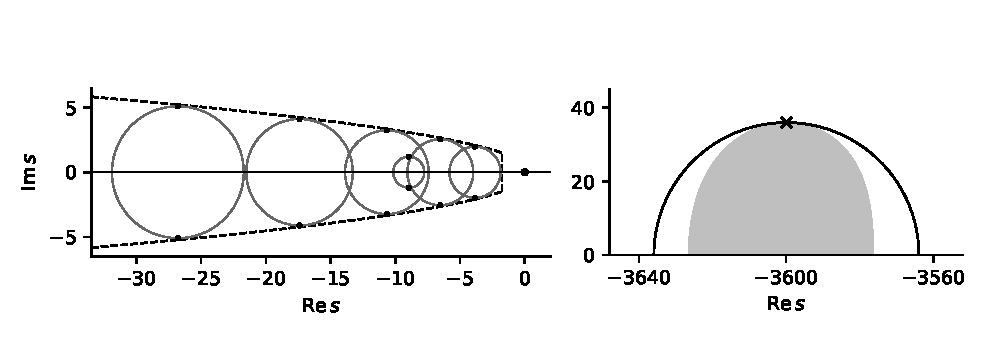
\includegraphics[width=\textwidth]{fig/pakes_disc.pdf}
\caption{Left: the sliver $\mathcal E_{T_0}$ of Theorem~\ref{bs:thm:local} for $T_0=2$ (dashed) and the discs $D_\gamma$ of six hypothetical zeros $a+ib$ with $a>2$ and $0<b<\frac12$, with the poles $-\gamma^2$ and $-\bar\gamma^2$ (dots) at the ends of their vertical diameters; the dot at $0$ marks the origin. Right: for the toy reciprocal Xi function with the first $200$ zeros of $\zeta$ and the pair $60\pm0.3i$, the set where $\Im\psi>0$ (shaded) on a grid of $481\times300$ points, which lies inside the upper half of $D_\gamma$ (solid); the cross is the pole $-\bar\gamma^2=-3599.91+36i$. Drawn by \texttt{pakes\_disc.py}.}
\label{bs:fig:disc}
\end{figure}

The threshold $p_*$ of Theorem~\ref{bs:thm:power} can be followed along the de Bruijn Newman flow. With $H_t$ and $\varphi_t(s)=H_t(0)/H_t(2i\sqrt s)$ as in Section~\ref{bh:sec:main}, so that $\varphi_0=\varphi$, let $\delta_*(t)$ be the largest angle $|\arg z|$ over the zeros $z$ of $H_t$ with $\Re z>0$, and $p_*(t)=1-2\delta_*(t)/\pi$. The proof of Theorem~\ref{bs:thm:power} uses only the product over the zeros, positivity on $(0,\infty)$ and the bound $|\arg z|<\pi/4$ required by Lemma~\ref{bs:lem:pair}, so whenever the zeros of $H_t$ satisfy that bound, $\varphi_t(x^p)$ is HCM if and only if $|p|\le p_*(t)$. By de Bruijn \cite{deBruijn} and Newman \cite{Newman1976} (Corollary~\ref{bh:cor:dbn}), $p_*(t)=1$ exactly for $t\ge\Lambda$; by Rodgers and Tao \cite{RodgersTao}, $p_*(t)<1$ for every $t<0$.

\begin{question}\label{bs:q:four}
Describe $p_*(t)=1-\frac2\pi\delta_*(t)$ for $t<0$. By Rodgers and Tao $p_*(t)<1$ for every $t<0$. Assume RH; how fast does $1-p_*(t)\to0$ as $t\uparrow0$?
\end{question}

Heuristically, the off line zeros of $H_t$ for small $|t|$ come from nearly coincident pairs of real zeros: by the isolated pair estimate of Section~\ref{ch:dbn}, a pair at distance $D_0$ collides near $t=-D_0^2/8$ and then has imaginary parts of order $\sqrt{|t|}$, at heights where the gap is of order $\sqrt{|t|}$. Since $1-p_*(t)$ is governed by $\max\Im z/\Re z$, the answer depends on the lowest height at which such a pair has collided, and so on the small gap statistics of the zeros. Both ingredients of an estimate are missing: de Bruijn's bound on the imaginary parts of the zeros runs only forward in time, from $H_0$ to $H_t$ with $t>0$, and no lower bound is known for the heights of the pairs that have collided by time $t$.

\subsection{The Thorin measure of $\varphi(s^p)$ and Bosch's variable}\label{bs:sec:thorin}

By Bondesson's theorem \cite[Theorem 6.1.1]{Bondesson}, a function with value $1$ at $0$ is HCM exactly when it is the Laplace transform of a GGC, so Theorem~\ref{bs:thm:power} already makes $\varphi(s^p)$ a GGC transform for $0<p\le p_*$.

\begin{theorem}\label{bs:thm:ggc}
Let $0<p\le p_*$. Then $\varphi(s^p)=\E e^{-sX_p}$ for a GGC variable $X_p$ with no drift. If $p<p_*$, its Thorin measure has the density
\begin{equation}\label{bs:eq:up}
u_p(\tau)=\frac{p}{\pi\tau}\,\Im\,\varepsilon_\varphi\bigl(\tau^pe^{ip\pi}\bigr)
=\frac{p}{2\pi\tau}\,\Im\Bigl[z\,\frac{\xi'}{\xi}\Bigl(\frac12+z\Bigr)\Bigr]_{z=\tau^{p/2}e^{ip\pi/2}}\ \ge0,\qquad\tau>0,
\end{equation}
which in terms of the zeros is
\begin{equation}\label{bs:eq:upzeros}
u_p(\tau)=\frac{p}{\pi\tau}\sum_\gamma\Im\frac{\tau^pe^{ip\pi}}{\tau^pe^{ip\pi}+\gamma^2}.
\end{equation}
If $p=p_*$, its Thorin measure is $u_{p_*}(\tau)\,d\tau$ plus a unit atom at $|\gamma|^{2/p_*}$ for every zero $\gamma$ with $\arg\gamma=-\delta_*$, counted with multiplicity, that is, one atom for each conjugate pair of zeros at the extreme angle; when $p_*=1$ there is an atom at $\gamma^2$ for every zero, and $u_1=0$.
\end{theorem}

\begin{proof}
Let $h=h_p$ and $\varepsilon_h(x)=p\,\varepsilon_\varphi(x^p)$. By the proof of Theorem~\ref{bs:thm:power}, $\varepsilon_h$ is analytic on $\Om$ and Pick. On $(0,\infty)$ it is nonnegative: a real zero contributes $x^p/(x^p+\gamma^2)>0$ and a pair contributes $2\Re\frac{s}{s+\varrho^2e^{2i\delta}}=\frac{2s(s+\varrho^2\cos2\delta)}{|s+\varrho^2e^{2i\delta}|^2}>0$. Hence $\varepsilon_h$ is complete Bernstein and $\varepsilon_h(x)/x=-(\log h)'(x)$ is a Stieltjes function, $a/x+b+\int U(dt)/(x+t)$. Here $a=\varepsilon_h(0+)=0$ and $b=\lim_{x\to\infty}\varepsilon_h(x)/x=0$ because $\varepsilon_\varphi(s)=O(\sqrt s\log s)$. Integrating from $0$ with $h(0)=1$ gives $h(x)=\exp(-\int\log(1+x/t)U(dt))$, a GGC transform. For $p<p_*$ the function $\varepsilon_h$ is continuous up to the upper edge of the cut, and Stieltjes inversion at $x=\tau e^{i\pi}$ gives $U(d\tau)=u_p(\tau)d\tau$ with $u_p(\tau)=\frac1{\pi\tau}\Im\varepsilon_h(\tau e^{i\pi})$, which is~\eqref{bs:eq:up};~\eqref{bs:eq:upzeros} follows from the Hadamard form of $\varepsilon_\varphi$. For $p=p_*$ the same inversion applies away from the points $x_0=\tau_0e^{i\pi}$ with $\tau_0=|\gamma|^{2/p_*}$ and $\arg\gamma=-\delta_*$, at which $x_0^{p_*}=-\gamma^2$. Near such a point the term of $\gamma$ in $\varepsilon_h$ is $p_*x^{p_*}/(x^{p_*}+\gamma^2)=x_0/(x-x_0)+O(1)$, so $\varepsilon_h(x)/x=1/(x+\tau_0)+O(1)$, and inversion gives a unit atom at $\tau_0$. On the ray itself this term equals $p_*\tau^{p_*}/(\tau^{p_*}-|\gamma|^2)$, which is real, so $u_{p_*}$ does not see the atom.
\end{proof}

\begin{corollary}\label{bs:cor:lamperti}
Let $L_p=Z_p/\tilde Z_p$ be the ratio of independent positive $p$ stable variables, whose density $\frac{\sin p\pi}{\pi}\,\frac{t^{p-1}}{t^{2p}+2t^p\cos p\pi+1}$ is Lamperti's \cite{boLamperti}; its power $L_p^{\,p}$ is Bosch's variable $T_\alpha$ with $\alpha=p$. Under RH the Thorin measure of $X_p$ is
\[
U_p=p\sum_\gamma\mathcal L\bigl(\gamma^{2/p}L_p\bigr),
\]
and $X_p\stackrel{d}{=}S_p\,X^{1/p}$, where $X=\sum_\gamma e_\gamma/\gamma^2$ is the clock variable of Proposition~\ref{prop:rigid}, with independent standard exponential variables $e_\gamma$, and $S_p$ is a positive $p$ stable variable independent of $X$ with $\E e^{-\lambda S_p}=e^{-\lambda^p}$. At $p=1/2$, $L_{1/2}\stackrel{d}{=}C^2$ for a standard Cauchy variable $C$, and $U_{1/2}=\frac12\sum_\gamma\mathcal L(\gamma^4C^2)$. As $p\uparrow1$, $L_p\to1$ and $U_p\to\sum_\gamma\delta_{\gamma^2}$ vaguely, the Thorin measure of $\varphi$ itself.
\end{corollary}

\begin{proof}
For real $\gamma$ the term of~\eqref{bs:eq:upzeros} equals $\frac{p}{\pi}\,\frac{\gamma^2\tau^{p-1}\sin p\pi}{\tau^{2p}+2\gamma^2\tau^p\cos p\pi+\gamma^4}$; substituting $\tau=\gamma^{2/p}t$ turns it into $p$ times Lamperti's density in $t$. The subordination identity is $\E e^{-sS_pY}=\E e^{-s^pY^p}$ with $Y=X^{1/p}$.
\end{proof}

Bosch's variable is therefore the kernel of the Thorin measure of $\varphi(s^p)$. Formula~\eqref{bs:eq:up} makes sense whatever the zeros are, and RH is the statement that it stays nonnegative as $p$ increases to $1$ (Question~\ref{bs:q:one} and the argument after it).

\begin{corollary}\label{bs:cor:rhX}
RH holds if and only if $X_p$ exists, that is $\varphi(s^p)$ is a GGC transform, for every $p\in(0,1)$. Unconditionally $X_p$ exists for $0<p\le1-1/(\pi T_0)$, in particular for $0<p\le1-1.1\times10^{-13}$, with the Thorin density~\eqref{bs:eq:up}.
\end{corollary}

\begin{proof}
If RH fails, $p_*<1$, and for $p\in(p_*,1)$ the function $\varphi(s^p)$ has a pole in $\Om$, which no GGC transform can have, since $\exp(-bs-\int\log(1+s/t)U(dt))$ is analytic and zero free on $\Om$. The rest is Theorem~\ref{bs:thm:ggc} with Corollary~\ref{bs:cor:uncond}, which gives $1-1/(\pi T_0)<p_*$.
\end{proof}

\begin{question}\label{bs:q:five}
Construct $X_{1/2}$ from Brownian motion, Bessel processes or the Biane, Pitman and Yor variables \cite{BPY01} without reference to the zeros. A construction that survived $p\uparrow1$ would prove RH by Corollary~\ref{bs:cor:rhX}.
\end{question}

\subsection{Positivity of the Thorin density from the primes}\label{bs:sec:open}

\label{bs:sec:limits}The method reads the threshold off the zeros: the elasticity has nonnegative imaginary part termwise on the sector $0<\arg s<\pi-2\delta_*$, and no information about $\delta_*$ is produced. A proof of RH along these lines must show $u_p\ge0$ for every $p<1$ directly from~\eqref{bs:eq:up}, for instance from the P\'olya kernel, from the prime sum of Remark~\ref{bs:rem:primes} or from a probabilistic model; this is the Thorin measure form of the reciprocal Xi programme of \cite{P17}. It cannot be done factor by factor: only the combination $(s-\frac14)\zeta(\frac12+\sqrt s)$ can enter an HCM or Pick argument (Section~\ref{bh:sec:use}).

\begin{question}\label{bs:q:one}
Prove $u_p\ge0$ for every $p\in(0,1)$ directly from~\eqref{bs:eq:up}, without locating the zeros.
\end{question}

The statement for all $p\in(0,1)$ is equivalent to RH. Under RH it holds by Theorem~\ref{bs:thm:ggc}. Conversely, suppose RH fails, let $\gamma=\varrho e^{i\delta_*}$ be a zero of maximal angle, and let $p\in(p_*,1)$; formula~\eqref{bs:eq:up} still defines $u_p$, except at isolated poles, although it is no longer a Thorin density. At $\tau=\varrho^{2/p}$ the term of $\bar\gamma$ in~\eqref{bs:eq:upzeros} equals $-\frac{p}{2\pi\tau}\cot\frac{\pi(p-p_*)}2$, which tends to $-\infty$ as $p\downarrow p_*$. The sum of the other terms stays bounded, because the other points $-\gamma'^2$ keep a positive distance from $-\bar\gamma^2$ and the tail of the sum is $O(\sum|\gamma'|^{-2})$. So $u_p$ takes negative values for $p$ slightly above $p_*$.

Along the ray write $\vartheta=p\pi/2\in(0,\pi/2)$, $t=\tau^{p/2}$, $z=te^{i\vartheta}$ and $w=\frac12+z$, so that $u_p(\tau)=\frac{p}{2\pi\tau}\Im[z\,\frac{\xi'}{\xi}(w)]$ by~\eqref{bs:eq:up}, and split $\xi'/\xi=\Gamma_\xi+\zeta'/\zeta$, where
\[
\Gamma_\xi(w)=\frac1w+\frac1{w-1}-\frac{\log\pi}2+\frac12\psi\Bigl(\frac w2\Bigr)
\]
is the logarithmic derivative of the factor $\frac12w(w-1)\pi^{-w/2}\Gamma(w/2)$ of $\xi$, and $\psi=\Gamma'/\Gamma$ is the digamma function, not the function $\psi$ of Theorem~\ref{bh:thm:main}. The ray crosses the critical strip for $t<t_e=1/(2\cos\vartheta)$ and then enters $\Re w>1$.

\begin{remark}[primes]\label{bs:rem:primes}
For $t>t_e$, that is $\tau>(2\cos(p\pi/2))^{-2/p}$, we have $\Re w>1$ and
\[
u_p(\tau)=\frac{p}{2\pi\tau}\Im\Bigl[z\Bigl(\frac1w+\frac1{w-1}-\frac{\log\pi}{2}+\frac12\psi\Bigl(\frac w2\Bigr)\Bigr)\Bigr]-\frac{p}{2\pi\tau}\sum_{n\ge2}\frac{\Lambda(n)}{\sqrt n}\,\Im\bigl(z\,n^{-z}\bigr),
\]
with $\Lambda$ the von Mangoldt function.
\end{remark}

\begin{proposition}\label{bs:prop:prime}
Let $\Re w>1$ and $\sigma=\Re w$. Then
\begin{equation}\label{bs:eq:primebound}
\frac{2\pi\tau}{p}\,u_p(\tau)\ \ge\ m_p(t):=\Im\Bigl[z\Bigl(\frac1{2w}+\frac1{w-1}+\frac12\log\frac{w}{2\pi}\Bigr)\Bigr]-\frac{t}{6\sigma^2}-t\Bigl(-\frac{\zeta'}{\zeta}\Bigr)(\sigma).
\end{equation}
Every term of $m_p$ is explicit, no zero of $\zeta$ enters, and $m_p(t)=\frac t2\sin\vartheta\log t\,(1+o(1))$ as $t\to\infty$. Consequently for each $p\in(0,1)$ there is $\tau_1(p)<\infty$ with $u_p(\tau)>0$ for all $\tau>\tau_1(p)$.
\end{proposition}

\begin{proof}
Binet's formula \cite[(5.9.13)]{DLMF} gives, for $\Re x>0$, $\psi(x)=\log x-\frac1{2x}-\int_0^\infty b(u)e^{-xu}du$ with $b(u)=\frac1{e^u-1}-\frac1u+\frac12\in[0,u/12]$. Hence $\psi(x)=\log x-\frac1{2x}-R$ with $|R|\le\frac1{12(\Re x)^2}$. With $x=w/2$ this turns $\Gamma_\xi(w)$ into $\frac1{2w}+\frac1{w-1}+\frac12\log\frac w{2\pi}-\frac R2$ with $|R|\le\frac1{3\sigma^2}$, so $\Im[z\Gamma_\xi(w)]$ is at least the first term of $m_p$ minus $t/(6\sigma^2)$. For the prime part, $\Im[z\,\zeta'/\zeta(w)]=-\sum\Lambda(n)\Im(zn^{-w})\ge-t\sum\Lambda(n)n^{-\sigma}$. The asymptotic follows from $\Im[z\log z]=t(\sin\vartheta\log t+\vartheta\cos\vartheta)$ and $-\zeta'/\zeta(\sigma)\to0$ as $\sigma\to\infty$.
\end{proof}

Table~\ref{bs:tab:prime} gives the point beyond which $m_p>0$, computed on a logarithmic grid of 50 points per decade, with $-\zeta'/\zeta(\sigma)$ evaluated directly. The entry $t_1$ is the last grid point at which $m_p\le0$, so the sign change lies within one grid step, a factor $10^{1/50}$, above it. These values are computed, not proved: nothing controls $m_p$ between grid points or beyond the last one.

The prime term of $m_p$ can be made elementary, because $-\zeta'/\zeta(\sigma)<1/(\sigma-1)$ for every $\sigma>1$. Delange \cite[Th\'eor\`eme]{Delange87} proves the sharper bound $-\zeta'/\zeta(\sigma)<1/(\sigma-1)-1/(2\sigma^2)$. Since $-\zeta'/\zeta(\sigma)$ enters $m_p$ with the factor $-t<0$, replacing it by $1/(\sigma-1)$ lowers $m_p$, and \eqref{bs:eq:primebound} still holds.

\begin{table}[h]
\centering
\begin{tabular}{ccccc}
\toprule
$p$ & strip exit $t_e=\frac1{2\cos\vartheta}$ & $t_1$ & $t_1/t_e$ & $\tau_1=t_1^{2/p}$\\
\midrule
$0.5$ & $0.707$ & $4.07$ & $5.75$ & $274$\\
$0.9$ & $3.20$ & $11.1$ & $3.47$ & $210$\\
$0.99$ & $31.8$ & $69.6$ & $2.19$ & $5.29\times10^3$\\
$0.999$ & $318$ & $553$ & $1.74$ & $3.10\times10^5$\\
$0.9999$ & $3183$ & $4818$ & $1.51$ & $2.33\times10^7$\\
\bottomrule
\end{tabular}
\caption{Where the lower bound~\eqref{bs:eq:primebound} becomes positive. On a logarithmic grid from $t_e$ to about $10^{14}t_e$, $m_p(t)>0$ at every grid point $t>t_1$; the ray reaches $t_1$ at $\tau_1=t_1^{2/p}$. The entries are computed, not proved.}
\label{bs:tab:prime}
\end{table}

\begin{remark}
The ratio $t_1/t_e$ tends to $1$. Near $\vartheta=\pi/2$ write $\sigma=1+x$, so $t=t_e(1+2x)$. The dominant terms of $m_p/t$ are $\frac12\log\frac t{2\pi}$ and $-\frac1x$, so positivity begins at $x\approx2/\log(t_e/2\pi)$, that is $t_1(p)=t_e(p)\bigl(1+\frac{4+o(1)}{\log(t_e/2\pi)}\bigr)$.
\end{remark}

So Question~\ref{bs:q:one} reduces, for each $p$, to the segment $|z|\le t_1(p)$ of the ray, which is asymptotically the part inside the critical strip. That part has length $t_e=1/(2\cos(p\pi/2))\approx1/(\pi(1-p))$, so heights and exponents correspond through $1-p\approx1/(\pi T)$, as in Corollary~\ref{bs:cor:uncond}.

\subsection{The density level and natural boundaries}

A variable with an HCM density is a GGC and so has an HCM Laplace transform ((F5) and (F6) of Section~\ref{bh:sec:bosch}). Under RH the clock variable $X=\sum_\gamma e_\gamma/\gamma^2$ is the GGC with transform $\varphi$. Its Cauchy counterpart is $X_C=\sum_ke_k/(2k-1)^2$, with transform $\sech(\pi\sqrt s/2)$.

\begin{theorem}\label{bs:thm:eta}
The density of $X_C$ is
\[
f_C(t)=\frac4\pi\sum_{k\ge1}(-1)^{k-1}(2k-1)e^{-(2k-1)^2t}=\frac4\pi\,\eta\Bigl(\frac{4it}{\pi}\Bigr)^3,\qquad t>0,
\]
with $\eta$ the Dedekind eta function. The line $\Re t=0$ is a natural boundary of $f_C$. Hence $X_C$ is a GGC whose Laplace transform is HCM, but the density of $X_C$ is not HCM.
\end{theorem}

\begin{proof}
The residue of $\sech(\pi\sqrt s/2)$ at $s=-(2k-1)^2$ is $\frac4\pi(-1)^{k-1}(2k-1)$, which gives the series once the Bromwich contour is moved to the left across the circles $|s|=4k^2$: for $s=4k^2e^{i\theta}$, $|\cosh(\pi\sqrt s/2)|^2=\sinh^2(\pi k\cos\frac\theta2)+\cos^2(\pi k\sin\frac\theta2)$ is at least $\frac14$ for every $\theta$ and at least $\sinh^2(\pi k/2)$ for $|\theta|\le2\pi/3$, while $|e^{st}|\le e^{-2k^2t}$ for $2\pi/3\le|\theta|\le\pi$, so for $t>0$ the integrals over the arcs of these circles to the left of the Bromwich line tend to $0$. Jacobi's identity $\eta(z)^3=\sum_{n\ge0}(-1)^n(2n+1)e^{\pi i(2n+1)^2z/4}$ \cite[Theorem 357]{boHardyWright}, at $z=4it/\pi$, where $e^{\pi i(2k-1)^2z/4}=e^{-(2k-1)^2t}$, gives the eta form. As a modular form $\eta$ has the real axis as natural boundary \cite[Chapter 11, Section 1.4, and Chapter 1, Section 4.2]{Remmert98}, and the real axis in $z$ is the line $\Re t=0$. An HCM density continues analytically to $\Om$ by~\eqref{bs:eq:bond}, so $f_C$ is not HCM.
\end{proof}

\begin{question}[density level]\label{bs:q:two}
Assume RH and that all zeros are simple. Does the density $f_X(t)=\sum_n A_n\gamma_n^2e^{-\gamma_n^2t}$ of $X$, with $A_n$ as in~\eqref{bh:eq:laplace}, have $\Re t=0$ as a natural boundary? If so, $X$ is not HCM.
\end{question}

P\'olya's gap theorem for Dirichlet series \cite{boPolya23,boPolya} says that if the exponents $\mu_n$ of a Dirichlet series $\sum_nc_ne^{-\mu_nt}$ have density $d=\lim n/\mu_n$ and satisfy $\inf_n(\mu_{n+1}-\mu_n)>0$, then every segment of length greater than $2\pi d$ on the line of convergence carries a singularity. When $\limsup\log n/\mu_n=0$ the abscissa of convergence equals $\limsup_n\log|c_n|/\mu_n$ \cite{boMandelbrojt}.

\begin{theorem}\label{bs:thm:nb}
Assume RH and that all zeros are simple, and assume
\begin{enumerate}
\item[(G)] $\inf_n(\gamma_{n+1}^2-\gamma_n^2)>0$;
\item[(D)] $\log\bigl(1/|\zeta'(\frac12+i\gamma_n)|\bigr)=o(\gamma_n^2)$.
\end{enumerate}
Then for $t>0$
\[
f_X(t)=\sum_nc_ne^{-\gamma_n^2t},\qquad c_n=A_n\gamma_n^2=-\frac{2\gamma_n\,\Xi(0)}{\Xi'(\gamma_n)},
\]
the series has abscissa of convergence $0$, and $\Re t=0$ is a natural boundary of $f_X$. In particular the density of $X$ is not HCM.
\end{theorem}

\begin{proof}
Residue expansion. The residue of $\varphi(s)=\Xi(0)/\Xi(i\sqrt s)$ at $s=-\gamma_n^2$ is $c_n$ as stated. Write $f_X$ as a Bromwich integral and move the contour to the left across the arcs of the circles $|s|=T_k^2$ that lie to the left of the Bromwich line, where, for large $k$, $T_k\in[k,k+1]$ is chosen at distance at least $c/\log k$ from every ordinate, with a small absolute constant $c>0$; this is possible because $[k-1,k+2]$ contains $O(\log k)$ ordinates \cite{HSW22}. Then $\zeta'/\zeta(\sigma+iy)=O(\log^2k)$ uniformly in $-1\le\sigma\le2$ and $|y-T_k|\le c/(2\log k)$ \cite[Theorem 9.6(A) and Section 14.4]{Titchmarsh}, and integration from $\sigma=2$ gives $1/|\zeta(\sigma+iy)|\le\exp(O(\log^2k))$ there. On the part of such an arc within angle $O(1/T_k)$ of the negative axis, $w=\frac12+\sqrt s$ has $\frac12\le\Re w\le2$ and $|\Im w|=\sqrt{T_k^2-(\Re w-\frac12)^2}=T_k+O(1/T_k)$, so for large $k$ it lies in this band or in its reflection in the real axis, and Stirling's formula gives $1/|\Xi(i\sqrt s)|\le\exp(O(T_k\log T_k))$, while $|e^{st}|\le e^{-tT_k^2/2}$. On the rest of the arc $\Re w\ge2$, and Stirling's formula gives $|e^{st}\varphi(s)|\le\exp\bigl(tT_k^2\cos\theta-\frac{T_k}2\cos\frac\theta2\log T_k+O(T_k)\bigr)$ for $s=T_k^2e^{i\theta}$. For $t>0$ both bounds tend to zero faster than any power of $T_k$, so the arcs contribute nothing in the limit and $f_X$ equals the residue series.

Abscissa. The exponents $\gamma_n^2$ satisfy $\log n/\gamma_n^2\to0$ and have density zero. By Stirling, $|\Xi'(\gamma_n)|=|\xi'(\rho_n)|=\gamma_n^{O(1)}e^{-\pi\gamma_n/4}|\zeta'(\rho_n)|$, so $\log|c_n|=\frac\pi4\gamma_n+O(\log\gamma_n)+\log(1/|\zeta'(\rho_n)|)$. Since $|\zeta'(\rho_n)|\le\gamma_n^{O(1)}$ always, (D) gives $\log|c_n|/\gamma_n^2\to0$, so the abscissa of convergence is $0$.

Natural boundary. By (G) and density zero, P\'olya's theorem places a singularity in every segment of the imaginary axis. An HCM density continues analytically to $\Om$, which contains the imaginary axis minus the origin.
\end{proof}

The same argument, with $\mu_k=(2k-1)^2$, gaps $8k$ and $c_k=\frac4\pi(-1)^{k-1}(2k-1)$, gives a second proof of Theorem~\ref{bs:thm:eta} that does not use modularity: by P\'olya's gap theorem \cite{boPolya23,boPolya} the line $\Re t=0$ is a natural boundary of $f_C$.

\begin{remark}[status of the hypotheses]
Hypothesis (D) is far weaker than the conjectured polynomial lower bounds for $|\zeta'(\rho)|$. Hypothesis (G) asks $\gamma_{n+1}-\gamma_n\ge c_0/(\gamma_n+\gamma_{n+1})$ for some $c_0>0$, a gap of order $1/\gamma$ against a mean spacing of order $1/\log\gamma$. Under the GUE model the expected number of violations is $\sum_n(\log\gamma_n/\gamma_n)^3<\infty$, so by the Borel Cantelli heuristic (G) fails at most finitely often, and then holds with a smaller $c_0$ if the zeros are simple.
\end{remark}

Numerically, for the first 200 zeros the coefficients $c_n$ computed from $\Xi'(\gamma_n)$ alternate in sign without exception; $\log|c_n|/\gamma_n^2$ equals $0.0462$, $0.0144$, $0.00524$, $0.00322$, $0.00195$ at $n=1,10,50,100,200$, tracking $\pi/(4\gamma_n)$; and the smallest gap $\gamma_{n+1}^2-\gamma_n^2$ is $159$, at $n=4$. The $c_n$ are the residues of the spectral expansion of the clock density in Section~\ref{ch:clocklaw}, written $R_k$ there, and Theorem~\ref{bs:thm:nb} describes, under its hypotheses, why that expansion cannot be continued past $t=0$.

For small $p$ the density of $X_p$ escapes this obstruction. The transform $\varphi(s^p)$ is analytic on the wider sector $|\arg s|<(\pi-2\delta_*)/p$ and, by Stirling's formula applied to $\xi(\frac12+z)$ for $|\arg z|<\pi/2$, decays along every ray strictly inside it. The inverse Laplace transform then continues the density of $X_p$ to the sector $|\arg t|<(\pi-2\delta_*)/p-\pi/2$, which contains $\Om$ when $p\le2p_*/3$.

\begin{question}\label{bs:q:three}
Determine $\{p:\ X_p\ \text{is HCM}\}$, and the same set for the Cauchy family $X_{C,p}$ with transform $\sech(\pi s^{p/2}/2)$.
\end{question}

Two facts constrain the answer. Under RH, $X_p\stackrel{d}{=}S_pX^{1/p}$, and positive $p$ stable variables are HCM exactly for $p\le1/2$, a conjecture of Bondesson \cite[Sections 5.7, 5.8 and 7.2]{Bondesson} proved by Bosch and Simon \cite[p.~32]{BoschSimon16}. Since HCM is preserved under products of independent variables and under powers of modulus at least one ((F1) and (F2) of Section~\ref{bh:sec:bosch}), HCM of $X$ would give HCM of $X_p$ for $p\le1/2$; but Theorem~\ref{bs:thm:nb} shows that $X$ is not HCM under (G) and (D), so this route is closed unless those hypotheses fail. The elasticity criterion reduces Question~\ref{bs:q:three} to the absence of zeros of the density $f$ of $X_p$ in $\Om$ and the Pick property of $-tf'(t)/f(t)$; by the continuation argument before Question~\ref{bs:q:three}, $f$ is at least analytic on $\Om$ for small $p$. A numerical scan of this elasticity for $X_{C,1/2}$ would be the first test.

\subsection{The Mellin variable $W$ and the first gap}

Question~\ref{bh:q:beta} asks for which $\beta$ the density of $W^\beta$ is HCM; on the Cauchy side the answer is $|\beta|\ge2$. Let $\chi(t)=\xi(\frac12)/\xi(\frac12+t)=\prod_\gamma(1+t^2/\gamma^2)^{-1}$ and let $g(y)=\frac1\pi\int_0^\infty\chi(t)\cos(ty)\,dt$ be the function $g$ of Section~\ref{bh:sec:dict}, which is entire because $\chi(t)=\exp(-\frac12|t|\log|t|(1+o(1)))$. By the van Dantzig pair of Section~\ref{ch:clock}, recalled in Section~\ref{bh:sec:dict}, $\chi$ is a characteristic function without RH: the clock variable $T$ exists unconditionally \cite[Theorem A]{P26}, and if $Z$ is a standard normal variable independent of $T$ then $\E e^{itZ\sqrt{2T}}=\E e^{-t^2T}=\chi(t)$. So $g$ is the density of the normal scale mixture $Z\sqrt{2T}$, and $W=\exp(Z\sqrt{2T})$ exists without any hypothesis. By the elasticity criterion, HCM of $W^\beta$ becomes a sign condition on $-g'/g$ in a strip (Proposition~\ref{bs:prop:Wcrit}), and since $g$ is entire no natural boundary stands in the way.

\subsubsection{A lower bound for $g$}

Theorem~\ref{bs:thm:gpos} proves the existence of $W$ a second time, independently of \cite[Theorem A]{P26}.

\begin{theorem}\label{bs:thm:gpos}
Unconditionally, by the verification of RH to height $T_0$ \cite{PT21}, $g(y)\ge0.9998\,g_R(y)>0$ for all real $y$, where $g_R$ is the density of $\sum_{\gamma\ \mathrm{real}}L_\gamma/\gamma$. Hence $\chi$ is a characteristic function and there is a positive random variable $W$ with $\E W^{it}=\chi(t)$ and $\E W^z=\Xi(0)/\Xi(z)$ for $|\Re z|<\gamma_1$.
\end{theorem}

\begin{proof}
Split $\chi=\chi_R\chi_{\mathrm{off}}$ into the products over real zeros and over conjugate pairs of nonreal zeros. For a pair $\gamma=\varrho e^{i\delta}=a+ib$ with $a,b>0$, the factor $(1+t^2/\gamma^2)^{-1}(1+t^2/\bar\gamma^2)^{-1}$ is the Fourier transform of the even kernel
\[
k_\gamma(x)=\frac{\varrho}{2\sin2\delta}\,e^{-a|x|}\sin(b|x|+\delta),
\]
of total mass one, positive for $|x|<(\pi-\delta)/b$ and bounded by $\frac{\varrho}{2\sin2\delta}e^{-a|x|}$. List the pairs as $\gamma^{(1)},\gamma^{(2)},\ldots$ in order of $\Re\gamma$, write $k_j=k_{\gamma^{(j)}}$, and let $\chi_m$ be the product of the first $m$ pair factors, $\nu_m=k_1*\cdots*k_m$ and $g_m=g_R*\nu_m$, the function with Fourier transform $\chi_R\chi_m$. We bound $g_m$ uniformly in $m$ and let $m$ grow at the end.

Comparison. $g_R=\ell*\tilde g_R$, where $\ell(z)=\frac{\gamma_1}2e^{-\gamma_1|z|}$ is the density of $L_{\gamma_1}/\gamma_1$ and $\tilde g_R$ is the density of the sum over the other real zeros, so $e^{-\gamma_1|x|}g_R(y)\le g_R(y-x)\le e^{\gamma_1|x|}g_R(y)$. Writing $\nu_m=\nu_m^+-\nu_m^-$,
\[
g_m(y)\ge g_R(y)\Bigl(\int e^{-\gamma_1|x|}\nu_m(x)dx-2\int\cosh(\gamma_1x)\,\nu_m^-(x)dx\Bigr)=:g_R(y)(A_m-2B_m).
\]

The term $A_m$. By Parseval, $A_m=\frac1\pi\int\chi_m(t)\frac{\gamma_1}{\gamma_1^2+t^2}dt=\E\,\chi_m(\gamma_1C)$ with $C$ a standard Cauchy variable. For $s\ge0$ each pair factor is $|1+s/\gamma^2|^{-2}\ge(1+s/\varrho^2)^{-2}\ge e^{-2s/\varrho^2}$, so $A_m\ge\E e^{-\kappa C^2}=e^\kappa\operatorname{erfc}(\sqrt\kappa)$ with $\kappa=2\gamma_1^2\Sigma_{\mathrm{off}}$ and $\Sigma_{\mathrm{off}}=\sum_{\mathrm{off}}|\gamma|^{-2}$. All nonreal zeros have $\Re\gamma>T_0=3\times10^{12}$ \cite{PT21}, so with $N(T)\le T\log T$ for $T\ge T_0$, $\Sigma_{\mathrm{off}}\le2\int_{T_0}^\infty N(T)T^{-3}dT\le2(\log T_0+1)/T_0<2\times10^{-11}$, $\kappa<8\times10^{-9}$ and $A_m>0.99989$.

The term $B_m$. For even signed measures $\int\cosh(\gamma_1x)\,d(|\mu|*|\nu|)=\int\cosh(\gamma_1 x)d|\mu|\cdot\int\cosh(\gamma_1x)d|\nu|$ exactly, and $(\mu*\nu)^-\le\mu^+*\nu^-+\mu^-*\nu^+$. Hence, with $M(\cdot)=\int\cosh(\gamma_1x)\,d(\cdot)$ and since $M(|k_\gamma|)\ge M(k_\gamma)=|1-\gamma_1^2/\gamma^2|^{-2}\ge1$,
\[
B_m\le\sum_{j\le m}M(k_j^-)\prod_{i\le m,\ i\ne j}M(|k_i|)\le SP,\qquad S=\sum_\gamma M(k_\gamma^-),\quad P=\prod_\gamma M(|k_\gamma|),
\]
with the sum and the product over all pairs. Here $k_\gamma^-$ lives on $|x|\ge(\pi-\delta)/b$ and $M(k_\gamma^-)\le\frac{\varrho}{\sin2\delta\,(a-\gamma_1)}\exp\bigl(-(a-\gamma_1)\frac{\pi-\delta}{b}\bigr)$. As $\varrho/\sin2\delta=\varrho^3/(2ab)$, this bound is $\frac{\varrho^3}{2a(a-\gamma_1)}\,b^{-1}e^{-K/b}$ with $K=(a-\gamma_1)(\pi-\delta)$. For fixed $a$ it increases with $b$: $\varrho$ increases, $K$ decreases because $\delta=\arctan(b/a)$ increases, and $b\mapsto b^{-1}e^{-K/b}$ increases on $(0,K)$. So, as $b<\frac12$, it is at most
\[
F(a)=\frac{(a^2+\frac14)^{3/2}}{a(a-\gamma_1)}\exp\Bigl(-2(a-\gamma_1)\bigl(\pi-\arctan\tfrac1{2a}\bigr)\Bigr),
\]
and $F(T_0)<\exp(-1.88\times10^{13})$, while $-(\log F)'>6$ on $[T_0,\infty)$. Every pair has $a>T_0$, so Stieltjes integration against $N(T)\le T\log T$ gives
\[
S\le F(T_0)\Bigl(T_0\log T_0+\frac{\log T_0+1}6+\frac1{36T_0}\Bigr)<\exp(-1.8\times10^{13}).
\]
Moreover $M(|k_\gamma|)=M(k_\gamma)+2M(k_\gamma^-)$ and $M(k_\gamma)\le\exp(3\gamma_1^2/\varrho^2)$, so $\log P\le3\gamma_1^2\Sigma_{\mathrm{off}}+2S<1.2\times10^{-8}$. So $A_m-2B_m>0.9998$ for every $m$.

Limit. For real $t$ each pair factor lies in $(0,1]$, and $\chi_R$ is integrable because it contains the factor $(1+t^2/\gamma_1^2)^{-1}$. By dominated convergence in the Fourier inversion integral, $g_m\to g$ uniformly on $\R$, so $g\ge0.9998\,g_R$. The comparison also gives $g_m(y)\le g_R(y)\int e^{\gamma_1|x|}|\nu_m(x)|dx\le2P\,g_R(y)$, since $e^{\gamma_1|x|}\le2\cosh(\gamma_1x)$ and $|\nu_m|\le|k_1|*\cdots*|k_m|$, so $g\le2P\,g_R$. Hence $g$ is integrable, its Fourier transform is $\chi$, and $\chi(0)=1$ makes $g$ a probability density. Finally $\int e^{cy}g_R(y)dy=\prod_{\gamma\ \mathrm{real}}(1-c^2/\gamma^2)^{-1}<\infty$ for $|c|<\gamma_1$, so $\int e^{c|y|}g(y)dy<\infty$ there, $\E W^z=\int e^{zy}g(y)dy$ is analytic on $|\Re z|<\gamma_1$, and it equals $\Xi(0)/\Xi(z)$ there because the two agree on the imaginary axis.
\end{proof}

The proof uses only that the zeros with $0<\Re\gamma\le T_0$ are real. The pair kernel formula and the constants of the proof were also checked numerically (\texttt{code/\allowbreak README.md}).

\subsubsection{Which powers of $W$ are HCM}

For real $\beta\ne0$ the density of $W^\beta$ is $x^{-1}g(\log x/\beta)/|\beta|$. With $y=\log x$, its elasticity is $1-\frac1\beta\frac{g'}{g}(y/\beta)$, and $x\in\C^+$ corresponds to $0<\Im y<\pi$; for $\beta<0$ the point $u=y/\beta$ then lies in the lower half of the strip $|\Im u|<\pi/|\beta|$, where the factor $\frac1\beta<0$ reverses the sign condition, and $g(\bar u)=\overline{g(u)}$, as $g$ is real on $\R$, moves it to the upper half. Theorem~\ref{bs:thm:crit} therefore gives the following.

\begin{proposition}\label{bs:prop:Wcrit}
Let $\beta\in\R\setminus\{0\}$. Then $W^\beta$ is HCM if and only if $g$ has no zeros in the strip $|\Im u|<\pi/|\beta|$ and $\Im\bigl(-g'(u)/g(u)\bigr)\ge0$ for $0<\Im u<\pi/|\beta|$.
\end{proposition}

As $\Im u\downarrow0$ the condition requires $(\log g)''\le0$ on $\R$; numerically $(\log g)''\le-2.2$ on $[0,1]$. On the Cauchy side $g_C=1/(\pi\cosh u)$, $-g_C'/g_C=\tanh u$, which is Pick on $0<\Im u<\pi/2$ with a pole at $i\pi/2$; Proposition~\ref{bs:prop:Wcrit} gives $|\beta|\ge2$, Bosch's theorem once more.

\begin{theorem}\label{bs:thm:gap}
Assume RH, simple zeros, and $\log(1/|\zeta'(\rho_n)|)=O(\gamma_n)$. Then $u_0=\frac\pi4+\limsup_n\gamma_n^{-1}\log(1/|\zeta'(\rho_n)|)$ is finite, and for $\Re u>u_0$
\[
g(u)=-\Xi(0)\sum_n\frac{e^{-\gamma_nu}}{\Xi'(\gamma_n)}=\sum_nb_ne^{-\gamma_nu},\qquad b_1>0>b_2,
\]
and if $W^\beta$ is HCM then $|\beta|\ge\gamma_2-\gamma_1=6.8873\ldots$.
\end{theorem}

\begin{proof}
The expansion is the residue computation for the Fourier integral $g(u)=\frac1{2\pi}\int\chi(t)e^{-itu}\,dt$ closed in the lower half plane. We move the line of integration to $\Im t=-T_k$, where $T_k\in[k,k+1]$ are heights at which $1/\zeta(\sigma\pm iT_k)=T_k^{O(1)}$ uniformly in $-1\le\sigma\le2$ \cite[Theorem 9.7]{Titchmarsh}; by Stirling's formula and the functional equation the moved integral is $O(e^{(\pi/4-\Re u)T_k+O(\log T_k)})$, which tends to $0$ for $\Re u>\pi/4$, so there $g(u)$ is the limit of the sums of the residue terms over $\gamma_n<T_k$. By Stirling, $\log|b_n|=\frac\pi4\gamma_n+\log(1/|\zeta'(\rho_n)|)+O(\log\gamma_n)$, so the series converges absolutely for $\Re u>u_0$, and $u_0\ge\pi/4$ because $|\zeta'(\rho_n)|\le\gamma_n^{O(1)}$, so its sum is $g(u)$ there (conjecturally $u_0=\pi/4$); the signs come from $b_n=\frac{\gamma_n}2A_n$. Put $\Delta=\gamma_2-\gamma_1$. As $\Re u\to\infty$ with $\Im u=v$ fixed,
\[
\Im\Bigl(-\frac{g'}{g}\Bigr)(x+iv)=\Delta\Bigl|\frac{b_2}{b_1}\Bigr|e^{-\Delta x}\sin(\Delta v)\,\bigl(1+O(e^{-cx})\bigr),\qquad c>0.
\]
For $\pi/\Delta<v<2\pi/\Delta$ this is negative for large $x$. If $|\beta|<\Delta$ the strip $0<\Im u<\pi/|\beta|$ contains such $v$, and Proposition~\ref{bs:prop:Wcrit} fails.
\end{proof}

\begin{question}[first gap conjecture]\label{bs:q:gap}
Is $W^\beta$ HCM exactly when $|\beta|\ge\gamma_2-\gamma_1$? On the Cauchy side the analogous statement, with frequencies $2k-1$, is Bosch's theorem at $\alpha=1/2$: $3-1=2$.
\end{question}

With $b_n$ computed from $\Xi'(\gamma_n)$ ($b_1=359.52$, $b_2=-28007$, $b_3=392918$) and $g$ computed by quadrature near the origin, a scan of $4840$ points with $0\le x\le6$ and $0<v<0.99\,v_*$, where $v_*=\pi/\Delta=0.45614$, found no value of $\Im(-g'/g)$ below $-1.3\times10^{-15}$, which is rounding; in 40 digit arithmetic the minimum over $1.1\le x\le9.1$ at $v=0.999\,v_*$ is $+1.0\times10^{-27}$. Just above the threshold the sign flips: the minimum is $-6.5\times10^{-8}$ at $v=1.001\,v_*$, so numerically the threshold is sharp to $0.1$ per cent.

Proving sufficiency requires the Pick property of $-g'/g$ in the full strip $0<\Im u<\pi/\Delta$, which near the origin is a statement about the P\'olya type kernel $g$ that does not reduce to the zeros.

\subsubsection{Solvable models}

To see whether the first gap rule is a coincidence of the half Cauchy case, we test it on a family in which everything is explicit. The logistic variable $\log W$ has characteristic function $\pi t/\sinh(\pi t)=\prod_{k\ge1}(1+t^2/k^2)^{-1}$. Removing a finite set $R$ of frequencies multiplies the characteristic function by $\prod_{k\in R}(1+t^2/k^2)$, which gives $g=\prod_{k\in R}(1-D^2/k^2)L$ with $D=d/dy$ and $L(y)=\frac14\sech^2(y/2)$. For each model we locate numerically the largest strip on which $\Im(-g'/g)\ge0$; by Theorem~\ref{bs:thm:crit}, as in Proposition~\ref{bs:prop:Wcrit}, its width $h_*$ gives the HCM threshold $\beta_*=\pi/h_*$. Table~\ref{bs:tab:gaps} lists the results.

\begin{table}[h]
\centering
\begin{tabular}{llccc}
\toprule
frequencies & gaps & first gap & largest gap & $\beta_*=\pi/h_*$\\
\midrule
$1,2,3,\ldots$ & $1,1,1,\ldots$ & 1 & 1 & $1.000$\\
$1,3,5,\ldots$ (half Cauchy) & $2,2,2,\ldots$ & 2 & 2 & $2$ (Bosch)\\
$1,3,4,5,\ldots$ & $2,1,1,\ldots$ & 2 & 2 & $2.000$\\
$1,3,5,6,\ldots$ & $2,2,1,\ldots$ & 2 & 2 & $2.000$\\
$1,3,4,6,\ldots$ & $2,1,2,1,\ldots$ & 2 & 2 & $2.000$\\
$1,4,5,6,\ldots$ & $3,1,1,\ldots$ & 3 & 3 & $3.000$\\
$1,4,5,7,\ldots$ & $3,1,2,1,\ldots$ & 3 & 3 & $3.000$\\
$1,4,7,8,\ldots$ & $3,3,1,\ldots$ & 3 & 3 & $3.000$\\
$1,5,6,7,\ldots$ & $4,1,1,\ldots$ & 4 & 4 & $4.000$\\
$1,2,4,5,\ldots$ & $1,2,1,\ldots$ & 1 & 2 & $1.269$\\
$1,2,3,6,\ldots$ & $1,1,3,1,\ldots$ & 1 & 3 & $1.317$\\
$1,2,5,6,\ldots$ & $1,3,1,\ldots$ & 1 & 3 & $1.483$\\
\bottomrule
\end{tabular}
\caption{HCM threshold for powers of $W$ in logistic models with frequencies removed, computed as $\beta_*=\pi/h_*$ from the width $h_*$ of the largest strip on which $\Im(-g'/g)\ge0$. The half Cauchy row is Bosch's theorem, not a computation.}
\label{bs:tab:gaps}
\end{table}

Whenever the first gap is at least as large as every later gap, the computed threshold equals the first gap, to the resolution of the computation. When some later gap exceeds the first, the threshold lies strictly between the first gap and the largest gap, and depends on where the large gap sits. The asymptotic argument of Theorem~\ref{bs:thm:gap} explains the lower bound in all cases. For the Riemann zeros the first gap $\gamma_2-\gamma_1=6.8873$ exceeds every later gap among the first $1000$ zeros (the next largest is $\gamma_4-\gamma_3=5.414$). The explicit form of the Riemann von Mangoldt formula of Hasanalizade, Shen and Wong, $|N(T)-\frac T{2\pi}\log\frac T{2\pi e}-\frac78|\le2.5167+\frac1{50T}$ for $e\le T\le X_0=30\,610\,046\,000$ and $\le0.1095\log T+0.2042\log\log T+3.0305+\frac1{50T}$ for $T>X_0$ \cite[(1.7), (2.7) and Corollary~1.4]{HSW22}, shows that every interval $(T,T+6.887]$ with $T\ge1000$ contains an ordinate: the lower bound it gives for the number of ordinates there exceeds $0.52$ at $T=1000$, increases with $T$ while $T+6.887\le X_0$, and exceeds $11$ beyond. So every gap that starts above height $1000$ is at most $6.887$, less than the first, and every gap that starts below it is a gap between two of the first $650$ zeros, since $N(1000)=649$. The first gap therefore exceeds every later gap. This refines Question~\ref{bs:q:gap}.

\begin{question}[first gap conjecture, refined]\label{bs:q:gaprefined}
Let $Y=\sum_nL_n/\lambda_n$ with independent standard Laplace variables $L_n$ and $0<\lambda_1<\lambda_2<\cdots$, and let $W=e^Y$. If the characteristic function of $Y$ decays faster than every exponential, or if the first gap $\lambda_2-\lambda_1$ is at least every later gap, is the HCM threshold of $W^\beta$ exactly $\lambda_2-\lambda_1$? In particular, is it $\gamma_2-\gamma_1$ for the Riemann variable?
\end{question}

\subsection{Where the difficulty lies}\label{bs:sec:discussion}

Bosch's theorem cannot be the input to a proof that the reciprocal Xi function is HCM, because for a product over the zeros HCM is equivalent to the reality of the zeros (Proposition~\ref{bh:prop:closure}), and Section~\ref{ch:sato} finds that every GGC criterion in the books of Sato and Bondesson is, at the centre, equivalent to RH. Bosch's method does transfer: at each of three levels it isolates one concrete object on which the question turns.

At the level of transforms the object is the Thorin density $u_p$ of~\eqref{bs:eq:up}. Its positivity for every $p<1$ is equivalent to RH; the primes prove it on each ray beyond some point, that point is asymptotically where the ray leaves the critical strip, and what remains is a segment of length about $1/(\pi(1-p))$. The first direction is to prove positivity on that segment from the explicit formula for $\xi'/\xi$ rather than from the zeros; computation alone extends the unconditional range $p\le1-1/(\pi T_0)$ only as fast as the verification height $T_0$ grows.

At the level of the Mellin variable the object is the sign of $\Im(-g'/g)$ in the strip $0<\Im u<\pi/(\gamma_2-\gamma_1)$. The second direction is to prove the first gap conjecture, first in the logistic models of Table~\ref{bs:tab:gaps}, where every quantity is elementary, and then for $W$, whose threshold the scan after Question~\ref{bs:q:gap} already locates to $0.1$ per cent. Question~\ref{bh:q:single} remains open.

At the level of densities the object is the natural boundary. The third direction is to establish it for the clock variable without the hypotheses (G) and (D) of Theorem~\ref{bs:thm:nb}, which would show what replaces, on the Riemann side, the modularity that produces the natural boundary on the Cauchy side.

Section~\ref{ch:heat} approaches the Thorin functional $\sum_\gamma\delta_{\gamma^2}$ of the clock, its Thorin measure under RH, from the other end of Bondesson's hierarchy, through its Laplace transform, the heat trace $W(t)=\sum_\gamma e^{-\gamma^2t}$.

\section{Exercises}\label{chap:hcm:ex}

\paragraph{On Section~\ref{ch:weak}.}
\begin{exercises}
\item Show that if $X_N$ are GGCs converging in law to a proper limit, the Thorin measures converge vaguely on $(0,\infty)$, and use the laws Gamma$(n,n)$ of Section~\ref{sec:ch3:readings}, which converge to the point mass at one, to show that Thorin mass escaping to infinity can reappear in the limit as drift.
\item For the sinh clock of Section~\ref{sec:ch3:bench} with one atom $k^2$ replaced by the conjugate pair $a,\bar a$, $a=-(\delta+ik)^2$ with $0<\delta<\frac12$, as in Proposition~\ref{prop:struct}, construct the Thorin densities at resolution $\varepsilon$ and show that their vague limit is the sinh measure with the atom $k^2$ removed.
\item Verify that $\varphi_{1/2}(uv)\varphi_{1/2}(u/v)=\prod_ka_k^2/(a_k^2+a_kuw+u^2)$ for the clock, and that at $u=|a|$ an off line pair contributes the completely monotone factor $(w+2\cos\arg a)^{-2}$.
\item Compute $(-1)^k\partial_w^kH_u(w)/H_u(w)$ for $k\le6$ at $u=1$ and $w=3$ from the P\'olya density and compare with Figure~\ref{fig:hcm}.
\end{exercises}

\chapter{The heat trace, the arithmetic and the limits of finite information}\label{chap:heat}\chaptermark{The heat trace and finite information}

Chapter~\ref{chap:hcm} worked at the top of the Bondesson hierarchy, with hyperbolic complete monotonicity, which for a Laplace transform is the GGC property; here we climb the hierarchy from the bottom. Every rung is a sign condition on the heat trace $W(t)$ of Section~\ref{ch:clock}, the pairing of the Thorin functional with $e^{-tz}$ (not the Mellin variable $W$ of Section~\ref{ch:boschB}). The lower rungs are unconditional theorems, proved with a finite verification of the zeros; the top rung is RH. Section~\ref{ch:heat} develops this hierarchy of positivity, and Section~\ref{ch:finite} shows what such finite information cannot decide. Section~\ref{ch:arith} computes the Thorin functional from the primes, and Section~\ref{ch:spacing} relates the errors of the P\'olya route on a window of finite height to the spacings of the zeros, which it compares with random matrix theory.

Taken together, Chapters~\ref{chap:measure} to \ref{chap:heat} show that on every window where the zeros are verified the computed Thorin measure converges to the RH measure at explicit rates, while above the computed range every finite computation of the kinds in this book remains consistent with a failure of the Thorin condition (Section~\ref{ch:finite}). Three of their threads return in Chapters~\ref{chap:basepoint} and \ref{chap:almost}: the count at resolution one half, which is the basepoint one (Section~\ref{ch:basepoint}), the self decomposability of the clock (Section~\ref{ch:sato}), and the zero density, whose classical estimates bound the negative Thorin mass below the basepoint one (Section~\ref{ch:almost}).

\section{The heat trace and the hierarchy of positivity}\label{ch:heat}

The rungs of the hierarchy proved unconditionally are infinite divisibility and self decomposability of the clock, log convexity of $W$, positive definite Hankel blocks up to size $3\times10^7$, the signs of all derivatives, equivalently the positivity of the Williamson measures, up to order $1.16\times10^{25}$, and near the origin the signs of every derivative: $W$ is completely monotone on $(0,1.29]$. One scheme proves them all, with a reach in size and order set by the height to which RH has been verified; no verification reaches the top, which is where Section~\ref{ch:finite} begins. The results are from \cite[Chapters 4 and 5]{P26} and \cite{P17}, except those stated without a citation, which are proved here.

\subsection{The heat trace and the first rungs}

By Section~\ref{ch:clock}, unconditionally,
\[
\log G(u)=\int_0^\infty\big(1-e^{-ut}\big)\frac{W(t)}t\,dt,\qquad W(t)=\sum_je^{-a_jt},
\]
where $a_j=-(\rho_j-\frac12)^2$ and the sum runs over one zero of each pair $\{\rho,1-\rho\}$. So $W(t)/t$ is the only candidate for the L\'evy density of the clock, and the classes of Section~\ref{ch:ggc} become conditions on $W$: nonnegativity for infinite divisibility, monotonicity for self decomposability, complete monotonicity for the GGC property.

The function $W$ is analytic in $\re t>0$, real on the positive axis, and can be differentiated term by term,
\[
c_k(t)=(-1)^kW^{(k)}(t)=\sum_ja_j^ke^{-a_jt}.
\]
Under RH every $c_k(t)$ is a sum of positive terms. A quadruple of zeros $\frac12\pm\delta\pm i\gamma$, $0<\delta<\frac12$, instead contributes the exponents $a=-(\delta+i\gamma)^2=\gamma^2-\delta^2-2i\delta\gamma$ and $\bar a$, hence the oscillating term $2|a|^ke^{-\re a\,t}\cos(2\delta\gamma t-k\phi)$, with $|a|=\gamma^2+\delta^2$ and $\tan\phi=2\delta\gamma/(\gamma^2-\delta^2)$. Its amplitude exceeds the contribution $2\gamma^{2k}e^{-\gamma^2t}$ of the same two zeros placed at $\frac12+i\gamma$ by the factor $(1+\delta^2/\gamma^2)^ke^{\delta^2t}\le\exp\{k\delta^2/\gamma^2+\delta^2t\}$ \cite[Proposition 11.1]{P17}.

\begin{resultpar}
As $t\downarrow0$ the archimedean term of \eqref{eq:ch2:Warith} dominates. Write $\vartheta$ for the Riemann Siegel theta function. Since $\re\psi(\frac14+\frac{iu}2)-\log\pi=2\vartheta'(u)$, the explicit formula gives, with no hypothesis,
\[
W(t)=e^{t/4}+\frac1\pi\int_0^\infty e^{-u^2t}\vartheta'(u)\,du-\frac1{\sqrt{4\pi t}}\sum_{n\ge2}\frac{\Lambda(n)}{\sqrt n}\,e^{-(\log n)^2/4t},
\]
and the prime terms are $O(t^{-1/2}e^{-(\log2)^2/4t})$, smaller than every power of $t$. Mellin's method for the integral \cite[Section 2.5]{DLMF} gives, for every $N$ and as $t\downarrow0$,
\[
W(t)=\frac{\log\frac1t-\gamma_E-4\log2-2\log\pi}{8\sqrt{\pi t}}+\sum_{n=0}^Nd_nt^n+\sum_{k=1}^Nb_kt^{k-\frac12}+O\big(t^{N+\frac12}\big),
\]
with $d_n=(1-\frac{E_{2n}}8)\frac{4^{-n}}{n!}$ and $b_k=\frac{(1-2k)\Gamma(\frac12-k)}{2\pi}\beta_k$, where $\gamma_E$ is Euler's constant, $E_{2n}$ are the Euler numbers and $\beta_k=\frac{(1-2^{1-2k})|B_{2k}|}{4k(2k-1)}$ are the coefficients of Stirling's series $\vartheta(u)\sim\frac u2\log\frac u{2\pi}-\frac u2-\frac\pi8+\sum_k\beta_ku^{1-2k}$. The terms $b_kt^{k-\frac12}$ come from the expansion of $\vartheta'$ at infinity, and the terms $d_nt^n$ from the Taylor series of $e^{-u^2t}$ through the Hurwitz value $\zeta(-2n,\frac14)=E_{2n}/4^{2n+1}$, together with the coefficients $4^{-n}/n!$ of $e^{t/4}$. After the leading term the series is $\frac78+\frac{\sqrt t}{48\sqrt\pi}+\frac9{32}t-\frac{7t^{3/2}}{2880\sqrt\pi}+\frac3{256}t^2+\frac{31t^{5/2}}{60480\sqrt\pi}+\frac{69}{3072}t^3+\cdots$, and it diverges; $\frac78=d_0$ is the constant of the Riemann von Mangoldt formula. The error of the two term expansion (the leading term and $\frac78$) is $b_1\sqrt t+d_1t+O(t^{3/2})$, which is $6.5\times10^{-4}$, $1.5\times10^{-4}$ and $4.0\times10^{-5}$ at $t=10^{-3},10^{-4},10^{-5}$ \cite[Corollary 5.5]{P17}; with the terms through $t^{5/2}$ the remainder agrees with $\frac{69}{3072}t^3$ to the order of the next term, $t^{7/2}$, in a $40$ digit computation for $10^{-6}\le t\le10^{-3}$, and at $t=10^{-2}$ it is $-8.377\times10^{-6}$, the prime $2$. Consequently $\int_\tau^\infty W(t)\,dt/t=\frac{\log\frac1\tau-\gamma_E-4\log2-2\log\pi-2}{4\sqrt{\pi\tau}}+\frac78\log\frac1\tau+O(1)$ as $\tau\downarrow0$, so the clock has infinitely many jumps. As $t\to\infty$ the first zero dominates, $W(t)=e^{-\gamma_1^2t}(1+o(1))$ with $\gamma_1^2=199.7904548$. In between, the arithmetic terms cancel to a depth that grows linearly in $t$ (Table~\ref{tab:ch2:W}).\label{tx3:res:wzero}
\end{resultpar}

\begin{theorem}[{\cite[Theorem A]{P26}}]\label{thm:ch12:idsd}
Unconditionally, that is, using only the verification of RH below height $1000$ \cite{PT21}, $W(t)>0$ and $W'(t)<0$ for every $t>0$. Consequently the clock is the Laplace transform of an infinitely divisible, self decomposable law with L\'evy density $W(t)/t$, and $(\Xi(\theta)/\Xi(0),\ \xi(\frac12)/\xi(\frac12+\theta))$ is a van Dantzig pair in the sense of Section~\ref{ch:clock}.
\end{theorem}

\begin{proof}
The proof is that of \cite[Theorem A]{P26}, with the constants made explicit. Let $\tau=1/20000$, a constant of this section only, $\ell=-\frac12\log t$, and $s_k(t)=\Gamma(k+\frac12)t^{-k-\frac12}/(4\pi)$, which is $(-1)^k$ times the $k$th derivative of $s_0(t)=1/(4\sqrt{\pi t})$. It suffices to show that $c_0$ and $c_1$ are positive, and we do so first for $t\le\tau$, from \eqref{eq:ch2:Warith}, and then for $t\ge\tau$, from the zeros.

Let $A$ and $P$ be the archimedean and prime terms of \eqref{eq:ch2:Warith}. The series $\psi(z)=-\gamma_E+\sum_{n\ge0}\big(\frac1{n+1}-\frac1{n+z}\big)$ \cite[(5.7.6)]{DLMF} shows that $m$ increases on $[0,\infty)$, from $m(0)=\psi(\frac14)-\log\pi=-\gamma_E-\frac\pi2-3\log2-\log\pi=-5.372$. Binet's formula $\psi(z)=\log z-\frac1{2z}-2\int_0^\infty v\,dv/\big((v^2+z^2)(e^{2\pi v}-1)\big)$ \cite[(5.9.15)]{DLMF} at $z=\frac14+\frac{ir}2$, with the integral split at $v=r/4$, gives $|m(r)-\log\frac r{2\pi}|\le\frac9{8r^2}+10^{-10}<0.003$ for $r\ge20$. Hence $|m|\le6$ on $[0,20]$ and $\int_0^{20}|m(r)-\log\frac r{2\pi}|\,dr\le120+4\pi+20\log\frac{10}\pi-20<136$. Since $\frac1{2\pi}\int_0^\infty r^{2k}e^{-r^2t}\log\frac r{2\pi}\,dr=s_k(t)(\ell+\alpha_k)$, with $\alpha_0=-\frac12\gamma_E-\log4\pi=-2.8196$ and $\alpha_1=\alpha_0+1$, it follows that
\[
\Big|\frac{(-1)^kA^{(k)}(t)}{s_k(t)}-\ell-\alpha_k\Big|\le\frac{272\cdot20^{2k}\,t^{k+\frac12}}{\Gamma(k+\frac12)}+0.003\qquad(k=0,1),
\]
and the right side, which increases with $t$, is below $1.089$ for $k=0$ and $0.047$ for $k=1$ at $t=\tau$. For the prime term put $y_n=(\log n)^2/4t$ and $q=(\log2)/8t$. Both $e^{-y_n}$ and $|y_n-\frac12|e^{-y_n}$ are at most $e^{-y_n/2}$, which is at most $n^{-q}$ because $(\log n)^2\ge(\log2)\log n$, and $\Lambda(n)\le\log n<\sqrt n$; so $|P^{(k)}(t)|\le(2\sqrt\pi)^{-1}t^{-k-\frac12}\sum_{n\ge2}n^{-q}<t^{-k-\frac12}2^{-q}$, that is $|P^{(k)}(t)|<t^{-k-\frac12}e^{-\kappa/t}$ for $k=0,1$ and $t\le\tau$, where $\kappa=(\log2)^2/8$ is another constant of this section. Since $\kappa/\tau>1201$, this is below $10^{-500}s_k(t)$. The polar term adds $e^{t/4}$ to $c_0$ and subtracts $\frac14e^{t/4}<10^{-5}s_1(t)$ from $c_1$. So for $t\le\tau$
\[
c_0(t)\ge s_0(t)\,(\ell-3.92),\qquad c_1(t)\ge s_1(t)\,(\ell-1.87),
\]
and both are positive, because $\ell\ge\frac12\log20000>4.95$.

For $t\ge\tau$ we use the zeros. Those below height $1000$ lie on the line \cite{PT21} and contribute $\gamma^{2k}e^{-\gamma^2t}>0$ to $c_k$, and by the explicit bound for $N(T)$ of \cite{HSW22} one of them lies in $(20,50]$ and contributes at least $400^ke^{-2500t}$. A zero above height $1000$, wherever it lies, has $\re a\ge\gamma^2-\frac14$ and $|a|\le2\gamma^2$. The same bound gives $N(r)\le r^2$ for $r\ge1000$, and integration by parts against $dN$ bounds the total modulus of the contributions of these zeros to $c_0$ and $c_1$ by
\[
H_0(t)=e^{-(10^6-\frac14)t}\big(10^6+t^{-1}\big),\qquad H_1(t)=2e^{-(10^6-\frac14)t}\big(10^{12}+2\cdot10^6t^{-1}+2t^{-2}\big).
\]
At $t=\tau$ these are below $2\times10^{-16}$ and $4.1\times10^{-10}$, while $e^{-2500\tau}>0.88$, and $e^{2500t}H_k(t)$ decreases with $t$. So $c_k(t)\ge400^ke^{-2500t}-H_k(t)>0$ for $t\ge\tau$ and $k=0,1$.

Thus $W>0$ and $W'<0$ on $(0,\infty)$. Since $0<W(t)\le\sum_je^{-t\re a_j}$, the measure $W(t)\,dt/t$ satisfies $\int_0^\infty(1\wedge t)\,W(t)\,dt/t\le\sum_j1/\re a_j<\infty$, so it is a L\'evy measure, and the formula for $\log G$ above makes the clock infinitely divisible with this L\'evy measure. A law on the half line whose L\'evy density is $W(t)/t$ with $W$ nonincreasing is self decomposable \cite[Corollary 15.11]{Sato99}. Finally, $\xi(\frac12)/\xi(\frac12+\theta)=\E e^{-\theta^2T}$ is the characteristic function of $Z\sqrt{2T}$, with $Z$ standard normal and independent of $T$, and with the characteristic function $\Xi(\theta)/\Xi(0)$ of the variable $X$ of Section~\ref{ch:clock} it forms a van Dantzig pair. The program \texttt{idsd\_check.py} (\texttt{code/\allowbreak README.md}) evaluates every numerical inequality of this proof in ball arithmetic.
\end{proof}

Tilting the clock by $e^{-T}$ gives $\xi(\frac32)/\xi(\frac12+\sqrt{1+s})=G(1)/G(1+s)=\E e^{-sT^{(1)}}$, with $T^{(1)}\ge0$ infinitely divisible, so unconditionally $h_k=\xi(\frac32)/\xi(\frac12+\sqrt{1+k})=\E(e^{-T^{(1)}})^k$ is a Hausdorff moment sequence.

The proof needs far fewer zeros than those below height $1000$. With the same bounds it goes through with $\tau=1/8300$ and the zeros below height $400$. If the archimedean error is bounded by computation instead, from $\int_0^5r^{2k}|m(r)-\log\frac r{2\pi}|\,dr<0.836$ and $0.404$ for $k=0,1$ and $r^2|m(r)-\log\frac r{2\pi}|<0.05$ for $r\ge5$, it goes through with $\tau=1/500$ and height $100$. If in addition the polar term $e^{t/4}$ is kept in $c_0$, the prime terms with $n\le30$ are taken exactly, and the lower bound for $t\ge\tau$ comes from the first zero, in $(14.1347,14.1348)$, rather than from a zero in $(20,50]$, it goes through with $\tau=1/50$ and height $25$, below which there are only two zeros. The program \texttt{idsd\_height.py} evaluates every numerical inequality of the three versions in ball arithmetic.

The same scheme, which we call the two range method, gives more. With the prime term bounded by $100\,t^{-k-\frac12}e^{-\kappa/t}$ for $k\le3$ and a second zero in $(100,200]$, it shows that $W$ and $-W'$ are strictly log convex \cite[Theorem 7.3]{P17}, that is $c_0c_2>c_1^2$ and $c_1c_3>c_2^2$ for every $t>0$, and that $(-1)^kW^{(k)}>0$ for $k\le3$.

For the first two rungs the explicit formula can be avoided altogether, because where the size of an off line quadruple cannot be bounded its phase fixes its sign, as the first author's note \cite{P26wig} observes. Suppose that the zeros with ordinate in $(0,H]$ lie on the line, with $H\ge100$, and let $0\le k\le H/8$. A quadruple $\frac12\pm\delta\pm i\gamma$ then has $\gamma>H$, and since $0<\phi<2\delta/\gamma<1/\gamma$ its phase satisfies $|2\delta\gamma t-k\phi|<\gamma t+1$, so its term in $c_k(t)$ is positive unless $\gamma t>\frac\pi2-1>0.57$. When $\gamma t>0.57$ the term is at most $2(\gamma^2+\frac14)^ke^{-(\gamma^2-\frac14)t}$ in modulus, and since $(\gamma^2+\frac14)/\gamma_1^2\le\gamma^2/99.9$, $\gamma^2-\frac14-\gamma_1^2\ge\gamma^2/2$ and $\gamma^2t/2>0.285\gamma$, it is at most $2(\gamma^2/99.9)^ke^{-0.285\gamma}$ times the term $\gamma_1^{2k}e^{-\gamma_1^2t}$ of the first zero. A quadruple has two zeros of ordinate $\gamma$, so at every $t>0$
\[
c_k(t)\ge\big(1-S_k(H)\big)\gamma_1^{2k}e^{-\gamma_1^2t},\qquad S_k(H)=\sum_{\gamma>H}\Big(\frac{\gamma^2}{99.9}\Big)^ke^{-0.285\gamma},
\]
the sum running over the zeros above height $H$, with multiplicity. The explicit bound for $N(T)$ of \cite{HSW22} gives $N(T+1)-N(T)<2\log T$ for $T\ge100$, and summing over unit intervals gives $S_0(100)<10^{-10.5}$ and $S_1(100)<10^{-8.5}$. Since Hutchinson placed the zeros below height $300$ on the line in 1925 \cite{Hutchinson25}, this proves Theorem~\ref{thm:ch12:idsd} without the explicit formula. For larger $k$ the factor $(\gamma^2/99.9)^k$ must be absorbed by $e^{-0.285\gamma}$ at $\gamma=H$, so the reachable order, about $0.285H/\log(H^2/99.9)$, stays below the height: the verification below $3\times10^{12}$ \cite{PT21} gives every $k\le10^{10}$, with $S_k(H)<10^{-1.4\times10^{11}}$. The two range method reaches orders proportional to $H^2$ (Theorems~\ref{thm:ch12:cm} and \ref{thm:ch12:window}). The program \texttt{ladder\_bound.py} evaluates these bounds in ball arithmetic.

Positivity of $W$ also limits how the clock factorises. By Mase's theorem \cite[Theorems 1 and 2]{Mase75}, an infinitely divisible law without Gaussian component whose L\'evy measure has a density that is positive on the whole half line, or that has mass on both half lines, has an indecomposable factor, hence a factor that is not infinitely divisible, so it lies outside Linnik's class $I_0$ \cite{Linnik64} of the infinitely divisible laws all of whose factors are infinitely divisible. Since $W>0$, this applies unconditionally to the clock variable $T$, to $Z\sqrt{2T}$ and to every nondegenerate GGC \cite[Proposition 12.1]{P17}.

\begin{proposition}[Truncation error]\label{tx:prop:trunc}
Let the zeros be simple, so that the $a_j$ are distinct, and let $r_k$ and $r_k^{(K)}$ be the residues at $u=-a_k$, $k\le K$, of $1/G(u)=\prod_ja_j/(a_j+u)$ and of its product over $j\le K$. Then $r_k=a_k\prod_{j\ne k}a_j/(a_j-a_k)$ and, when $|a_j|>|a_k|$ for $j>K$,
\[
\log\frac{r_k^{(K)}}{r_k}=\sum_{j>K}\log\Big(1-\frac{a_k}{a_j}\Big)=-a_k\sum_{j>K}a_j^{-1}-\frac{a_k^2}2\sum_{j>K}a_j^{-2}-\cdots.
\]
Under RH $a_j=\gamma_j^2$ and $\sum_{j>K}\gamma_j^{-2}\sim\log\gamma_K/(2\pi\gamma_K)$, so the first term is $-\gamma_k^2\log\gamma_K/(2\pi\gamma_K)$: the truncated coefficient is close to the residue for $\gamma_k\le(\gamma_K/\log\gamma_K)^{1/2}$, and not beyond.
\end{proposition}

\begin{proof}
The product converges absolutely, and its pole at $-a_k$ is simple, with residue $a_k$ times the other factors at $u=-a_k$. The ratio of the two residues is the tail product $\prod_{j>K}(a_j-a_k)/a_j$. For the sum, $\sum_{j>K}\gamma_j^{-2}=\int_{\gamma_K}^\infty T^{-2}\,dN(T)$ with $N(T)=\frac T{2\pi}\log\frac T{2\pi}-\frac T{2\pi}+O(\log T)$, which is $(\log(\gamma_K/2\pi)+1)/(2\pi\gamma_K)$ to leading order.
\end{proof}

\subsection{Hankel blocks and derivative signs}

Fix $t>0$ and form the Hankel matrices $[c_{i+j}(t)]$ and $[c_{i+j+1}(t)]$, $i,j\ge0$.

\begin{theorem}[{\cite[Theorem 7.1]{P17}}]\label{thm:ch12:hankel}
For any fixed $t>0$ the following are equivalent: both infinite Hankel matrices are positive semidefinite; Weil's quadratic form is positive semidefinite on the span of $r^me^{-r^2t/2}$, $m=0,1,2,\dots$; RH.
\end{theorem}

Under RH the derivatives at one time are the moments of the positive measure $e^{-tz}U(dz)$ on the half line, so both matrices are positive semidefinite. Conversely, if both Hankel matrices are positive semidefinite, Stieltjes' theorem makes the $c_k(t)$ the moments of a positive measure $\mu$ on the half line, and since $\sum_kc_k(t)(-s)^k/k!=W(t+s)$ for $|s|<t$, $W(t+s)=\int e^{-sx}\mu(dx)$ there. Both sides are analytic in $\re s>-t$, the right side because $\int e^{|s|x}\mu(dx)=\sum_kc_k(t)|s|^k/k!=W(t-|s|)<\infty$ for $|s|<t$, so the identity theorem extends the equality to $\re s>-t$, and $W$ is completely monotone, which is RH. Through the explicit formula, Weil's form on the span of $r^me^{-r^2t/2}$ gives the same two matrices, even $m$ the first and odd $m$ the second.

Theorem~\ref{thm:ch12:hankel} tests RH on the real axis. The next one tests it on the vertical line, where $W$ is a sum of oscillating terms.

\begin{theorem}\label{tx:thm:vertical}
RH holds if and only if $v\mapsto W(\sigma+iv)$ is bounded on $\R$, for one, equivalently every, $\sigma>0$.
\end{theorem}

\begin{proof}
Write $s_j=-a_j=(\rho_j-\frac12)^2=x_j+iy_j$, $\rho_j=\frac12+\delta_j+i\gamma_j$, so that $x_j=\delta_j^2-\gamma_j^2$, $y_j=2\delta_j\gamma_j$, $|\delta_j|<\frac12$, $|y_j|\le|\gamma_j|$ and $\gamma_j\ne0$. Only three facts on the zeros are used: $|\delta_j|<\frac12$, $\gamma_j\ne0$ ($\xi$ has no zeros in $(0,1)$) and $N(T)=O(T\log T)$, so that $\sum_je^{-c\gamma_j^2}<\infty$ for every $c>0$ and only finitely many $|\gamma_j|$ lie below any height. Put $F(v)=W(\sigma+iv)=\sum_jc_je^{is_jv}$, $c_j=e^{s_j\sigma}$, $C=\sum_j|c_j|\le e^{\sigma/4}\sum_je^{-\sigma\gamma_j^2}<\infty$. Since $|e^{is_jv}|=e^{-y_jv}\le e^{|\gamma_jv|}$, the series converges absolutely and locally uniformly in $v$.

Under RH every $s_j=-\gamma_j^2$ is real, so $|F(v)|\le\sum_je^{-\sigma\gamma_j^2}=W(\sigma)$ for every $\sigma>0$. Conversely let $|F|\le M$ on $\R$ for one $\sigma$, and suppose RH fails. For $\omega\in\R$ and complex $\varepsilon$ with $\re\varepsilon>0$ put $L(\varepsilon)=\int_\R F(v)e^{-\varepsilon v^2-i\omega v}\,dv$.

Step 1. On $\re\varepsilon\ge\eta>0$ the integrand is entire in $\varepsilon$ and bounded by $Me^{-\eta v^2}$, so $L$ is continuous by dominated convergence and holomorphic by Morera's theorem, with Fubini over triangles justified by the same bound. For real $\varepsilon>0$, $|L(\varepsilon)|\le M\sqrt{\pi/\varepsilon}$.

Step 2. For $\varepsilon>0$ and $b\in\mathbb C$, $\int_\R e^{-\varepsilon v^2+bv}\,dv=\sqrt{\pi/\varepsilon}\,e^{b^2/4\varepsilon}$: both sides are entire in $b$ and agree for real $b$ by completing the square. With $b=i(s_j-\omega)$ this gives $\int_\R e^{is_jv-\varepsilon v^2-i\omega v}\,dv=\sqrt{\pi/\varepsilon}\,e^{-(s_j-\omega)^2/4\varepsilon}$. The sum over $j$ may be taken under the integral (Fubini and Tonelli) if $\sum_j|c_j|\int_\R e^{-y_jv-\varepsilon v^2}\,dv=\sqrt{\pi/\varepsilon}\sum_je^{\sigma\delta_j^2-\sigma\gamma_j^2+\delta_j^2\gamma_j^2/\varepsilon}<\infty$. For real $\varepsilon\ge1/(2\sigma)$ we have $\delta_j^2/\varepsilon\le\sigma/2$, each term is at most $e^{\sigma/4}e^{-\sigma\gamma_j^2/2}$, and the sum is finite. Hence $L(\varepsilon)=\sqrt{\pi/\varepsilon}\,\Psi_\varepsilon(\omega)$ for $\varepsilon\ge1/(2\sigma)$, where $\Psi_\varepsilon(\omega)=\sum_jc_je^{-(s_j-\omega)^2/4\varepsilon}$ and the root is principal.

Step 3. The series $\Psi_\varepsilon(\omega)$ converges locally uniformly on $\re\varepsilon>0$. Let $K$ be compact there. Then $u=1/(4\varepsilon)$ stays in a compact set with $\re u\ge u_0>0$ and $|\im u|\le u_1$. Write $(s_j-\omega)^2=X+iY$ with $X=(x_j-\omega)^2-y_j^2$ and $Y=2(x_j-\omega)y_j$. For $\gamma_j^2\ge\frac14+|\omega|$ we have $|x_j-\omega|\ge\gamma_j^2-\frac14-|\omega|$, so $X\ge(\gamma_j^2-\frac14-|\omega|)^2-\gamma_j^2$ and $|Y|\le2|\gamma_j|(\gamma_j^2+\frac14+|\omega|)$, of orders $\gamma_j^4$ and $|\gamma_j|^3$. Hence there is $G=G(K,\omega)$ such that $X>0$ and $u_0X-u_1|Y|\ge0$ for $|\gamma_j|\ge G$, and then $|e^{-(X+iY)u}|=e^{-(X\re u-Y\im u)}\le e^{-(u_0X-u_1|Y|)}\le1$, so the $j$th term is at most $|c_j|$. Only finitely many $j$ have $|\gamma_j|<G$, and $\sum_j|c_j|=C$, so the M-test applies and $\Psi$ is holomorphic on $\re\varepsilon>0$. Now $L$ and $\sqrt{\pi/\varepsilon}\,\Psi_\varepsilon(\omega)$ are holomorphic on the connected half plane and agree on $[1/(2\sigma),\infty)$, so by the identity theorem they agree throughout. With Step 1,
\[
|\Psi_\varepsilon(\omega)|\le M\qquad(\varepsilon>0,\ \omega\in\R).\tag{$*$}
\]

Step 4. Put $t=1/(4\varepsilon)$ and $q_j(\omega)=y_j^2-(x_j-\omega)^2$. Then $|e^{-(s_j-\omega)^2t}|=e^{q_jt}$ and its phase is $e^{-i\phi_jt}$, $\phi_j=2(x_j-\omega)y_j$. For fixed $\omega$ and level $l$ only finitely many $j$ have $q_j(\omega)\ge l$, because $q_j\le\gamma_j^2-(\gamma_j^2-\frac14-|\omega|)^2\to-\infty$ as $|\gamma_j|\to\infty$.

Step 5. Take a zero off the line, with $s_0=x_0+iy_0$, $y_0=2\delta\gamma\ne0$. On the open interval $I_0=(x_0-|y_0|,x_0+|y_0|)$, $q_0>0$. For two values $s\ne s'$ in $\{s_j\}$ with $(x,|y|)\ne(x',|y'|)$, the difference $q-q'=y^2-y'^2-x^2+x'^2+2\omega(x-x')$ is a nonconstant affine function of $\omega$ if $x\ne x'$ and a nonzero constant if $x=x'$, so it vanishes for at most one $\omega$. Let $E$ be the countable set of these points together with $\{x_j\}$, and fix $\omega\in I_0\setminus E$. By Step 4, $Q=\max_jq_j(\omega)$ is attained, $Q\ge q_0>0$, and by the choice of $\omega$ every maximiser has the same $(x,|y|)$, so $s_j\in\{s^*,\bar s^*\}$ for a fixed $s^*=x^*+iy^*$. Now $Q>0$ forces $y^*\ne0$, and $\omega\ne x^*$ forces $\phi:=2(x^*-\omega)y^*\ne0$. Only finitely many $j$ have $q_j\ge0$, so $Q'=\max\{0,\,q_j(\omega):s_j\notin\{s^*,\bar s^*\}\}$ is a maximum over a finite set and $Q'<Q$.

Step 6. Let $m_1\ge1$ and $m_2\ge0$ be the numbers of $j$ with $s_j=s^*$ and $s_j=\bar s^*$, and $A=e^{s^*\sigma}\ne0$. The terms with $\bar s^*$ have the same $q$, the phase $e^{+i\phi t}$ and the coefficient $\bar A$. Hence $\Psi_\varepsilon(\omega)=e^{Qt}g(t)+r(t)$ with $g(t)=m_1Ae^{-i\phi t}+m_2\bar Ae^{i\phi t}$ and $|r(t)|\le\sum_j|c_j|e^{Q't}=Ce^{Q't}$ for $t>0$. The function $g$ is continuous and periodic with period $2\pi/|\phi|$, and not identically zero, since its Fourier coefficient at the frequency $-\phi\ne\phi$ is $m_1A\ne0$. So $\kappa=\max|g|>0$ is attained in every period, at points $t_k\to\infty$, and with $\varepsilon_k=1/(4t_k)$, using $Q>0$ for the growth and $Q>Q'$ for the remainder,
\[
|\Psi_{\varepsilon_k}(\omega)|\ge\kappa e^{Qt_k}-Ce^{Q't_k}\to\infty,
\]
contradicting $(*)$. So RH holds. Since boundedness for one $\sigma$ gives RH, and RH gives it for every $\sigma$, the two readings agree.
\end{proof}

\begin{theorem}[{\cite[Theorem 7.4]{P17}}]\label{thm:ch12:blocks}
If all zeros below $T_N=20000N\sqrt{1+\log N}$ are on the line, the leading $N\times N$ blocks are positive definite at every $t>0$. The verification to height $3\times10^{12}$ \cite{PT21} gives this for every $N\le3\times10^7$.
\end{theorem}

Table~\ref{tab:ch12:hankel} shows normalised leading minors recomputed in sixty digit arithmetic from the first $1700$ zeros, whose ordinates are stored in double precision; they agree with \cite[Numerical observation 7.2]{P17} to every digit printed there.

\begin{table}[htbp]
\centering\small
\begin{tabular}{rllllll}
\toprule
$t$ & $c_0c_2/c_1^2$ & $N=2$ & $N=3$ & $N=4$ & $N=5$ & block\\
\midrule
0.01 & 1.1346548 & 0.119 & $2.45\times10^{-3}$ & $1.05\times10^{-5}$ & $1.04\times10^{-8}$ & even\\
0.01 & & 0.182 & $5.87\times10^{-3}$ & $3.30\times10^{-5}$ & $4.57\times10^{-8}$ & odd\\
0.05 & 1.0000081 & $8.11\times10^{-6}$ & $1.77\times10^{-14}$ & $5.35\times10^{-28}$ & $2.20\times10^{-44}$ & even\\
0.05 & & $1.79\times10^{-5}$ & $1.22\times10^{-13}$ & $1.71\times10^{-26}$ & $3.81\times10^{-42}$ & odd\\
\bottomrule
\end{tabular}
\caption{Normalised leading Hankel minors of the heat trace, $\det[c_{i+j}]_{i,j<N}/\allowbreak\prod_{i<N}c_{2i}$ for the even block and $\det[c_{i+j+1}]_{i,j<N}/\allowbreak\prod_{i<N}c_{2i+1}$ for the odd block, from the first $1700$ zeros in sixty digit arithmetic.}
\label{tab:ch12:hankel}
\end{table}

At $t=0.05$ (Figure~\ref{fig:ch12:hankel}, left) the first exponents dominate and the others enter only through $e^{-(a_j-a_1)t}$, so the matrix is nearly of rank one. Computed from the zeros, the minors are still sums of positive terms, by the Cauchy Binet formula $\det[c_{i+j}]_{i,j<N}=\sum_{|S|=N}\prod_{l\in S}e^{-a_lt}\prod_{l<l',\ l,l'\in S}(a_l-a_{l'})^2$ over the sets $S$ of $N$ zeros, so what is lost is conditioning, not sign. The derivative signs (Figure~\ref{fig:ch12:hankel}, right) reach much further, because a sign needs only that the verified terms dominate, not that a small determinant stay positive.

\begin{figure}[htbp]
\centering
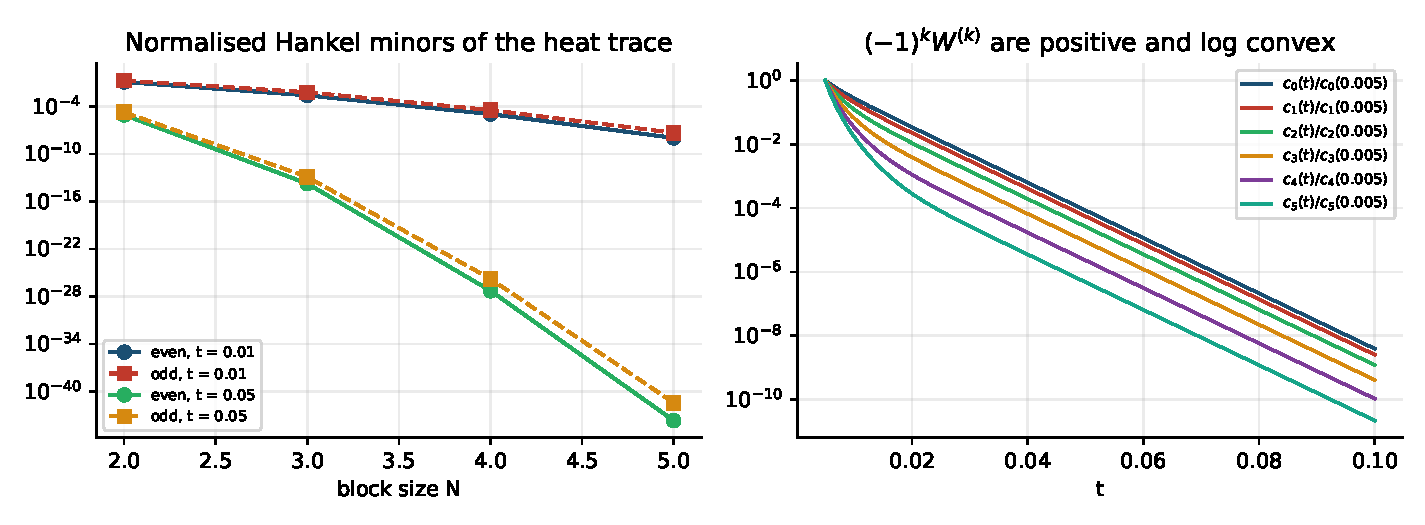
\includegraphics[width=\textwidth]{fig/hankel.pdf}
\caption{Left: normalised Hankel minors of the heat trace at two times; positivity persists but falls below any fixed precision as $t$ grows. Right: the first six $(-1)^kW^{(k)}(t)$, divided by their values at $t=0.005$, from $1700$ zeros.}
\label{fig:ch12:hankel}
\end{figure}

\begin{theorem}[{\cite[Theorem 7.10]{P17}}]\label{thm:ch12:cm}
Unconditionally, that is, using only the verification of RH below height $10^{12}$ \cite{PT21}, $(-1)^kW^{(k)}(t)>0$ for every $t>0$ and every integer $0\le k\le10^{17}$.
\end{theorem}

The proof again splits at $\tau$. Near the origin, Cauchy's estimate on a circle about $t$ of radius close to $t$, such as $(1-\frac1{k+1})t$, on which $\re(1/z)\ge1/(2t)$ and $|z|\ge t/(k+1)$, bounds the $k$th derivative of the prime term by a multiple of $(k+1)\Gamma(k+\frac12)t^{-k-\frac12}e^{-\kappa/t}$. Against $s_k(t)$ this loses a factor of order $k$ and gains $e^{-\kappa/t}\le e^{-1201}$, and for $k\ge1$ the archimedean term dominates by a margin of more than $2.9\,s_k(t)$, the case $k=0$ being Theorem~\ref{thm:ch12:idsd}. Away from the origin a zero in $(20,50]$ dominates all zeros above the verified height $H=10^{12}$, wherever they lie, provided $tH^2\ge2(k+1)$ and a logarithmic condition hold; Section~\ref{sec:ch12:reach} explains why these allow orders up to about $10^{18}$.

The Stieltjes moments of Table~\ref{tab:ch3:diag} give a Hankel test at the other end of the heat trace, and the test also returns the zeros \cite{P26wig}. They are the moments of $W$, $m_n=\frac1{n!}\int_0^\infty t^nW(t)\,dt=\sum_ja_j^{-n-1}$, and since $\log G(u)=\sum_j\log(1+u/a_j)=\sum_{n\ge1}(-1)^{n+1}m_{n-1}u^n/n$ they follow from the Taylor coefficients of $G(u)=\Xi(i\sqrt u)/\Xi(0)=\sum_kM_ku^k/((2k)!\,M_0)$, where $M_k=\int_\R v^{2k}\Phi(v)\,dv$; no zero enters. Under RH the $m_n$ are the moments of the positive measure $\nu=\sum_ja_j^{-1}\delta_{1/a_j}$, so every Hankel matrix $\mathcal H_N=[m_{i+j}]_{i,j<N}$ is positive definite. Conversely, if all of them are, Hamburger's theorem makes the $m_n$ the moments of a positive measure, of compact support because $|m_n|\le\sum_j|a_j|^{-n-1}$ grows at most geometrically, and then $\sum_nm_nw^n=\sum_j1/(a_j-w)$ has all its poles on the real axis: every $a_j$ is real, and positive because $\xi$ has no zeros in $(0,1)$, which is RH. The shifted matrices $\mathcal H'_N=[m_{i+j+1}]_{i,j<N}$ give the same test, and either suffices alone: if every $\mathcal H'_N$ is positive definite, Hamburger's theorem applied to $(m_{n+1})$ and $\sum_nm_nw^n=m_0+w\sum_nm_{n+1}w^n$ give the same conclusion. Positivity is tested by the Cholesky factorisation $\mathcal H_N=LL^\top$, and the factor gives more: $J_N=L^{-1}\mathcal H'_NL^{-\top}$ is the Jacobi matrix of $\nu$, tridiagonal, and its eigenvalues are the nodes of the $N$ point Gauss rule for $\nu$. They approximate the largest atoms $1/a_j$ first, so their inverse square roots return the lowest ordinates (Table~\ref{tab:ch12:jacobi}). With $M_0,\dots,M_{100}$ computed at $1000$ digits by the trapezoid rule, every $\mathcal H_N$ up to order $50$ is positive definite.

\begin{table}[htbp]
\centering\small
\begin{tabular}{rrllll}
\toprule
$N$ & zeros & error of $\gamma_1$ & last error & $\det\mathcal H_N/\det\mathcal H_{N-1}$ & digits\\
\midrule
$10$ & $2$ & $4.4\times10^{-18}$ & $1.3\times10^{-9}$ & $2.0\times10^{-61}$ & $60$\\
$20$ & $7$ & $1.6\times10^{-49}$ & $3.1\times10^{-7}$ & $1.2\times10^{-138}$ & $140$\\
$30$ & $12$ & $8.6\times10^{-87}$ & $2.4\times10^{-7}$ & $1.0\times10^{-221}$ & $230$\\
$40$ & $17$ & $6.1\times10^{-128}$ & $5.4\times10^{-8}$ & $1.3\times10^{-308}$ & $310$\\
$50$ & $22$ & $5.3\times10^{-172}$ & $5.4\times10^{-8}$ & $1.4\times10^{-398}$ & $400$\\
\bottomrule
\end{tabular}
\caption{The lowest ordinates from the Stieltjes moments $m_0,\dots,m_{2N-1}$, computed from the Taylor coefficients of $\Xi$ at the centre: the number returned by the Jacobi matrix of order $N$ to within $10^{-6}$, the errors of the first and of the last of them, the last Cholesky pivot of $\mathcal H_N$, and the least number of digits, in steps of $10$, of the Taylor coefficients and of the arithmetic from which on the same ordinates are returned.}
\label{tab:ch12:jacobi}
\end{table}

This is Gauss quadrature, equivalently Pad\'e approximation of $G'/G$ at the origin, and Table~\ref{tab:ch12:jacobi} shows its two limits. The first is precision. The last Cholesky pivot $\det\mathcal H_N/\det\mathcal H_{N-1}$ falls from $10^{-61}$ at $N=10$ to $10^{-398}$ at $N=50$, and the computation must resolve it. The precision thus grows linearly, by about $17$ digits for each further zero. The second is reach. An off line quadruple at height $\gamma$ enters $m_n$ with weight of order $\gamma^{-2n-2}$, against $\gamma_1^{-2n-2}$ for the first zero, so a block of order $N$ sees essentially only the zeros that its Gauss rule resolves; Section~\ref{sec:ch21:hankel} shows this along the de Bruijn Newman flow, where the order $30$ test registers the collision of the pair just above the zeros it resolves, and not a collision higher up. The program \texttt{jacobi\_zeros.py} computes the table.

The Hankel matrices count the zeros off the line as well as test RH. For a real polynomial this is a theorem attributed to Hermite \cite{Hermite1856}: the Hankel form of the power sums of the roots has as many negative squares as the polynomial has distinct pairs of nonreal roots. Let $\iota_N$ and $\iota'_N$ be the numbers of negative eigenvalues of $\mathcal H_N$ and $\mathcal H'_N$.

\begin{theorem}\label{thm:ch12:inertia}
Let $K\in\{0,1,2,\dots\}\cup\{\infty\}$ be the number of distinct zeros $\rho$ of $\xi$ with $\re\rho>\frac12$ and $\im\rho>0$. Then $\iota_N$ and $\iota'_N$ are nondecreasing in $N$, $\iota_N\le K$ and $\iota'_N\le K$ for every $N$, and $\iota_N\to K$ and $\iota'_N\to K$ as $N\to\infty$. In particular RH holds if and only if $\iota_N=0$ for every $N$, and if it fails, $\iota_N\ge1$ from some $N$ on; the same holds for $\iota'_N$.
\end{theorem}

\begin{proof}
Put $b_k=1/a_k$, listed with multiplicity, so that $m_n=\sum_kb_k^{n+1}$ and $\sum_k|b_k|<\infty$. For a real vector $x=(x_0,\dots,x_{N-1})$ and $P(w)=\sum_ix_iw^i$,
\[
x^\top\mathcal H_Nx=\sum_kb_kP(b_k)^2,\qquad x^\top\mathcal H'_Nx=\sum_kb_k^2P(b_k)^2,
\]
the sums converging absolutely. A zero on the line gives $b_k=\gamma_k^{-2}>0$ and nonnegative terms. A zero $\rho=\frac12+\delta+i\gamma$ with $\delta>0$ and $\gamma>0$, of multiplicity $\mu$, gives $a=-(\delta+i\gamma)^2$ with $\im a=-2\delta\gamma<0$, hence $b=1/a$ with $\im b>0$; its mirror image $1-\bar\rho$ gives $\bar a$ and $\bar b$ with the same multiplicity, and since $P$ has real coefficients the two contribute $2\mu\re\big(bP(b)^2\big)$ to the first form. With $u=\re P(b)$ and $v=\im P(b)$ this is $2\mu\big(\re b\,(u^2-v^2)-2\im b\,uv\big)$, a quadratic form in $(u,v)$ whose matrix has determinant $-4\mu^2|b|^2<0$, so it has exactly one negative square, and composed with the linear map $x\mapsto(u,v)$ it has at most one. The terms of the zeros on the line add up to a positive semidefinite form, so $\iota_N\le K$. In the second form the weight is $b^2$, and $2\mu\re\big(b^2P(b)^2\big)$ is again a form in $(u,v)$ of determinant $-4\mu^2|b|^4<0$, so $\iota'_N\le K$. Since $\mathcal H_N$ is the leading principal submatrix of $\mathcal H_{N+1}$, Cauchy's interlacing theorem shows that $\iota_N$ does not decrease, and the same holds for $\iota'_N$.

For the lower bound let $\mathcal B$ be the closure of $\{b_k\}$. It is a countable compact set, symmetric under conjugation, whose only possible accumulation point is $0$, and a countable compact set does not separate the plane, so $\C\setminus\mathcal B$ is connected. Fix a finite $m\le K$ and distinct atoms $\omega_1,\dots,\omega_m$ with $\im\omega_j>0$, of multiplicities $\mu_j$; they are isolated points of $\mathcal B$. On $\C^m=\R^{2m}$ the form $q(y)=\sum_{j\le m}2\mu_j\re(\omega_jy_j^2)$ is a sum of $m$ forms in the pairs $(\re y_j,\im y_j)$, each with one negative square, so there are an $m$ dimensional real subspace $E$ and $\lambda_0>0$ with $q(y)\le-\lambda_0|y|^2$ on $E$. Let $y^{(1)},\dots,y^{(m)}$ be a basis of $E$ and $\lambda_1>0$ such that $|\sum_i\alpha_iy^{(i)}|^2\ge\lambda_1|\alpha|^2$ for $\alpha\in\R^m$. Take open discs $D_j$ about $\omega_j$, and their mirror images $D_j^*$ about $\bar\omega_j$, whose closures are disjoint and meet $\mathcal B$ only in their centres, and an open set $O\supset\mathcal B\setminus\{\omega_1,\bar\omega_1,\dots,\omega_m,\bar\omega_m\}$, symmetric under conjugation and disjoint from the closed discs, which exists because that set is compact. Let $f_i$ be $y^{(i)}_j$ on $D_j$, $\overline{y^{(i)}_j}$ on $D_j^*$ and $0$ on $O$. Each $f_i$ is holomorphic on a neighbourhood of $\mathcal B$, so by Runge's theorem there are polynomials $\tilde P_i$ with $|\tilde P_i-f_i|<\varepsilon$ on $\mathcal B$, and since $\mathcal B$ and $f_i$ are symmetric under conjugation, $P_i(w)=\frac12\big(\tilde P_i(w)+\overline{\tilde P_i(\bar w)}\big)$ has real coefficients and satisfies the same bound. For $\alpha\in\R^m$ and $P=\sum_i\alpha_iP_i$ we have $|P(b_k)|\le\varepsilon\sqrt m\,|\alpha|$ at every atom other than the $\omega_j$ and $\bar\omega_j$, and $P(\omega_j)=\sum_i\alpha_iy^{(i)}_j+\eta_j$ with $|\eta_j|\le\varepsilon\sqrt m\,|\alpha|$. The atoms $\omega_j$ and $\bar\omega_j$ contribute $\sum_j2\mu_j\re\big(\omega_jP(\omega_j)^2\big)$ to the first form, so for $\varepsilon\le1$ and a constant $C$ that depends on neither $\varepsilon$ nor $\alpha$,
\[
\sum_kb_kP(b_k)^2\le q\Big(\sum_i\alpha_iy^{(i)}\Big)+C\varepsilon|\alpha|^2\le-(\lambda_0\lambda_1-C\varepsilon)|\alpha|^2 .
\]
For $\varepsilon<\lambda_0\lambda_1/C$ the right side is negative for $\alpha\ne0$, so the coefficient vectors of $P_1,\dots,P_m$ span an $m$ dimensional space on which the form of $\mathcal H_N$ is negative definite as soon as $N$ exceeds their degrees, and $\iota_N\ge m$ for those $N$. For $\mathcal H'_N$ the same argument applies with $\omega_j^2$ in place of $\omega_j$ in $q$ and the weights $b_k^2$ in the sum. Since $m\le K$ is arbitrary, $\iota_N\to K$ and $\iota'_N\to K$.
\end{proof}

In determinant form the theorem is classical. For a real entire function of order one with zeros $z_j$, Grommer \cite{Grommer14} proved that all its zeros are real if and only if the determinants $D_n=\det(s_{i+j})_{i,j<n}$ of the power sums $s_k=\sum_jz_j^{-k-2}$ are positive for every $n\ge1$, and Chebotarev \cite{Chebotarev28} that if the sequence $D_{n-1}D_n$, $n\ge1$, with $D_0=1$, has exactly $m$ negative terms, the function has $m$ distinct pairs of complex conjugate zeros; Baricz and \v{S}tampach state both in this form \cite[Theorem 10]{BS18}. For $\Xi$, whose zeros are the square roots of the $a_k$, $s_{2l}=2m_l$ and $s_{2l+1}=0$, so after the even indices are put first $(s_{i+j})_{i,j<n}$ is block diagonal with the blocks $2\mathcal H_{\lceil n/2\rceil}$ and $2\mathcal H'_{\lfloor n/2\rfloor}$, whose negative indices add up to $\iota_{\lceil n/2\rceil}+\iota'_{\lfloor n/2\rfloor}$; this tends to $2K$, and each zero $\rho$ counted by $K$ gives two pairs of complex conjugate zeros of $\Xi$, as Chebotarev's count requires. Counting by eigenvalues rather than by the signs of determinants, Theorem~\ref{thm:ch12:inertia} needs no determinant to be nonzero, allows $K=\infty$ and holds for each family separately. Along the de Bruijn Newman flow the proof applies at every time to the zeros of $H_t$, none of which is purely imaginary (Section~\ref{sec:ch21:hankel}).

\subsection{Every order near the origin}\label{sec:ch12:allorders}

Let $s_k(t)=\Gamma(k+\frac12)t^{-k-\frac12}/(4\pi)$ as in the proof of Theorem~\ref{thm:ch12:idsd}, let $E_k(t)$ be the average of $m$ against the weight $r^{2k}e^{-r^2t}$ on $[0,\infty)$, and let $F_k(x)={}_1F_1(k+\frac12;\frac12;-x^2)$. Expanding the cosine in its power series gives $\frac1{2\pi}\int_{\R}r^{2k}e^{-r^2t}\cos(ry)\,dr=2s_k(t)F_k(y/2\sqrt t)$, whose case $k=0$ is the kernel $e^{-y^2/4t}/(2\sqrt{\pi t})$ of the prime term of \eqref{eq:ch2:Warith}. Differentiating \eqref{eq:ch2:Warith} $k$ times term by term, which the Gaussian factors in $r$ and in $\log n$ allow, therefore gives, with no hypothesis on the zeros,
\begin{equation}\label{eq:ch12:ckarith}
\frac{c_k(t)}{s_k(t)}=E_k(t)-2\sum_{n\ge2}\frac{\Lambda(n)}{\sqrt n}F_k(x_n)+\frac{(-\frac14)^ke^{t/4}}{s_k(t)},\qquad x_n=\frac{\log n}{2\sqrt t}.
\end{equation}
In \eqref{eq:ch12:ckarith} the archimedean term $E_k(t)$ grows with $k$.

\begin{lemma}\label{lem:ch12:hermite}
\textup{(a)} For every integer $k\ge0$ and every $x\ge0$, $|F_k(x)|\le B(x)e^{-x^2/2}$, where $B(x)=\max\{2.62,\ (\pi(2ex^2+\frac12))^{1/4}\}$.

\textup{(b)} Let $0<\varepsilon<1$, and let $k\ge1$ and $x\ge0$ satisfy $e^2x^2\le4\varepsilon k$. Then $|F_k(x)|\le C_\varepsilon(k)e^{-x^2/2}$, where $C_\varepsilon(k)=\sqrt{(k+0.37)/((1-\varepsilon)k+\frac14)}+2\sqrt{k+0.37}\,e^{-\varepsilon k}$.
\end{lemma}

\begin{proof}
Taking $t=1$ and $y=2x$ above, $F_k(x)=\Gamma(k+\frac12)^{-1}\int_{\R}r^{2k}e^{-r^2+2ixr}\,dr$. Put $\mu=x^2/4$. The integrand is entire and decays in every horizontal strip, so the path can be moved to $\im r=x/2$, where $|r^{2k}|=(\sigma^2+\mu)^k$, $|e^{-r^2}|=e^{-\sigma^2+\mu}$ and $|e^{2ixr}|=e^{-4\mu}$, with $\sigma=\re r$. Expanding $(\sigma^2+\mu)^k$ by the binomial theorem gives, for every $k$ and $x$,
\[
|F_k(x)|\le e^{-3\mu}\sum_{j=0}^k\frac{\mu^j}{j!}P_{k,j},\qquad P_{k,j}=\frac{\Gamma(k+1)}{\Gamma(k+\frac12)}\,\frac{\Gamma(k-j+\frac12)}{\Gamma(k-j+1)}.
\]
Kershaw's inequalities $\sqrt{y+\frac14}\le\Gamma(y+1)/\Gamma(y+\frac12)\le\sqrt{y+0.37}$, proved for $y>0$ in \cite{Kershaw83} and true at $y=0$, where the ratio is $1/\sqrt\pi$, give $P_{k,j}\le\sqrt{(k+0.37)/(k-j+\frac14)}$, which is less than $\sqrt2$ for $j\le k/2$ and at most $2\sqrt{k+0.37}$ for every $j$. For (a), suppose first that $k\ge2ex^2$. Since $k/2\ge4e\mu$, Chernoff's bound $\sum_{j\ge a}\mu^j/j!\le(e\mu/a)^a$ for the Poisson law, valid for $a>\mu$, gives $\sum_{j\ge k/2}\mu^j/j!\le(2e\mu/k)^{k/2}\le2^{-k}$, and $2\sqrt{k+0.37}\,2^{-k}\le\sqrt{1.37}<1.2$ for $k\ge1$. Hence $|F_k(x)|\le e^{-3\mu}(\sqrt2\,e^\mu+1.2)\le(\sqrt2+1.2)e^{-x^2/2}$, and $\sqrt2+1.2<2.62$; for $k=0$ the assumption forces $x=0$, where $F_0=1$.

Suppose now that $k<2ex^2$. Kummer's transformation and the Hermite case of ${}_1F_1$ \cite[(13.2.39), (13.6.16)]{DLMF} give $F_k(x)=e^{-x^2}{}_1F_1(-k;\frac12;x^2)=(-1)^k\frac{k!}{(2k)!}e^{-x^2}H_{2k}(x)$, and the bound $e^{-x^2/2}|H_n(x)|\le(2^nn!)^{1/2}$ \cite[(18.14.9)]{DLMF} gives
\[
|F_k(x)|\le\Big(\frac{4^k(k!)^2}{(2k)!}\Big)^{1/2}e^{-x^2/2}\le\big(\pi(k+\tfrac12)\big)^{1/4}e^{-x^2/2}<\big(\pi(2ex^2+\tfrac12)\big)^{1/4}e^{-x^2/2},
\]
since $4^k(k!)^2/(2k)!=\sqrt\pi\,\Gamma(k+1)/\Gamma(k+\frac12)\le\sqrt{\pi(k+\frac12)}$ by Kershaw's upper bound.

For (b), split the sum at $j=\varepsilon k$ instead. For $j\le\varepsilon k$, $P_{k,j}\le\sqrt{(k+0.37)/((1-\varepsilon)k+\frac14)}$, and these $j$ contribute at most that times $e^\mu$. For $j>\varepsilon k$, $P_{k,j}\le2\sqrt{k+0.37}$, and since $\varepsilon k\ge e^2\mu>\mu$, Chernoff's bound gives $\sum_{j\ge\varepsilon k}\mu^j/j!\le(e\mu/\varepsilon k)^{\varepsilon k}\le e^{-\varepsilon k}$. Hence $|F_k(x)|\le e^{-3\mu}\big(\sqrt{(k+0.37)/((1-\varepsilon)k+\frac14)}\,e^\mu+2\sqrt{k+0.37}\,e^{-\varepsilon k}\big)\le C_\varepsilon(k)e^{-x^2/2}$.
\end{proof}

\begin{theorem}\label{thm:ch12:cmint}
\textup{(a)} For every integer $k\ge1$ and every $t\in(0,0.019]$, $(-1)^kW^{(k)}(t)>0$. The proof uses no information on the zeros.

\textup{(b)} Unconditionally, that is, using only the verification of RH below height $10^{12}$ \cite{PT21}, $W$ is completely monotone on $(0,1.29]$: $(-1)^kW^{(k)}(t)>0$ for every $t\in(0,1.29]$ and every integer $k\ge0$.
\end{theorem}

\begin{proof}
By \eqref{eq:ch12:ckarith} and Lemma~\ref{lem:ch12:hermite}(a), for every $k\ge0$ and $t>0$,
\[
\frac{c_k(t)}{s_k(t)}\ge E_k(t)-S_B(t)-Q_k(t),
\]
where
\[
S_B(t)=2\sum_{n\ge2}\frac{\Lambda(n)}{\sqrt n}B(x_n)e^{-(\log n)^2/8t},\qquad Q_k(t)=\frac{4\pi e^{t/4}t^{k+\frac12}}{4^k\,\Gamma(k+\frac12)}.
\]
Above the order $K=10^{17}$ part (b) of the lemma does better. Take $\varepsilon=10^{-6}$. The first term of $C_\varepsilon(k)$ decreases in $k$, because $\frac14<0.37(1-\varepsilon)$, and the second decreases for $k>1/(2\varepsilon)$, so $C_\varepsilon(k)\le C=C_\varepsilon(K+1)<1+6\times10^{-7}$ for $k>K$, and $e^2x^2\le4\varepsilon k$ holds for $x\le2\sqrt{\varepsilon(K+1)}/e$, which exceeds $2.3\times10^5$. For $t\ge0.019$ every prime power $n\le2^{24}$ has $x_n<61$. So for $k>K$ and $t\ge0.019$ the bound holds with $S_B$ replaced by $S_C$, the sum $S_B$ with $B(x_n)$ replaced by $C$ for $n\le2^{24}$.

The three terms are monotone. Since $m$ increases on $[0,\infty)$, and the weights $r^{2k}e^{-r^2t}$ have likelihood ratios $r^2$ from $k$ to $k+1$ and $e^{r^2(t'-t)}$ from $t'$ to $t<t'$, both increasing in $r$, $E_k(t)$ increases in $k$ and decreases in $t$. $Q_k(t)$ increases in $t$, and for $t\le2$ it decreases in $k$, the ratio of consecutive terms being $t/(4k+2)$. $B(x)e^{-x^2/2}$ decreases on $(0,\infty)$: the second branch of $B$ increases and is $1.78$ at $x=2^{-1/2}$, so $B=2.62$ below that point, and above it the logarithmic derivative of the second branch times $e^{-x^2/2}$ is less than $1/(2x)-x<0$; since $x_n$ decreases in $t$, $S_B$ and $S_C$ increase in $t$. So for $k\ge k_0$ and $t\le T\le2$ each bound is at least its value at $(k_0,T)$, and it suffices to prove $E_1(0.019)-S_B(0.019)-Q_1(0.019)>0$, which gives (a), and $E_{K+1}(1.29)-S_C(1.29)-Q_{K+1}(1.29)>0$, which gives the orders $k>K$ on $[0.019,1.29]$; with (a) for $t\le0.019$ and Theorem~\ref{thm:ch12:cm} for the orders $k\le K$, this gives (b).

For the first, lower sums over $[0,64]$, which the monotonicity of $m$ allows, and the positivity of $m$ beyond $64$ give $E_1(0.019)>0.15924$; the prime powers $n\le30000$ and the tail bound below give $S_B(0.019)<0.13628$; and $Q_1(0.019)<0.00933$. For the second, the weight $r^{2K+2}e^{-r^2t}$ makes $v=r^2t$ a gamma variable of shape $\lambda=K+\frac32$, and Chernoff's bound for the gamma law, $\Pr(v<a)\le(a/\lambda)^\lambda e^{\lambda-a}$ for $a<\lambda$, gives $\Pr(v<a)<e^{-1000}$ for $a=(1-2^{-13})^2\lambda$. As $m$ increases, $E_{K+1}(t)\ge m(r_1)-(m(r_1)-m(0))e^{-1000}$ with $r_1=\sqrt{a/t}$, which gives $E_{K+1}(1.29)>17.6066$; the prime powers $n\le2^{24}$ and the tail bound below give $S_C(1.29)<17.5848$; and $Q_{K+1}(1.29)<e^{-1000}$. In both cases the prime powers above the cutoff $n_0$, which is $30000$ and $2^{24}$, add less than $2\big(2.62+2.08(2\sqrt t)^{-1/2}\big)n_0^{1-q}/(q-1)$ with $q=\log n_0/8t$, because $x_n\ge x_{n_0}\ge1$ and $e^{-(\log n)^2/8t}\le n^{-q}$ for $n>n_0$, $B(x)\le2.62+2.08\sqrt x$ for $x\ge1$, and $\log n$ and $(\log n)^{3/2}$ are at most $\sqrt n$ for $n\ge e^{10}$; this is below $10^{-299}$ and $5\times10^{-4}$. The program \texttt{cm\_orders.py} evaluates every numerical inequality of this proof and of the proof of Lemma~\ref{lem:ch12:hermite} in ball arithmetic.
\end{proof}

Computed in floating point, the bound $E_1-S_B-Q_1$ of (a) vanishes at $t=0.0193$; $E_1$ itself vanishes at $t=0.0261$, so no bound on the size of the prime terms carries (a) much further. Part (b) goes further because $E_k(t)=\frac12(\psi(k+\frac12)-\log t)-\log2\pi+O(t/k)$ grows like $\frac12\log k$, while at such orders part (b) of the lemma bounds the prime terms at almost no cost: the bound $E_{K+1}-S_C$, computed in the same way, vanishes at $t=1.2912$, while $E_{K+1}-S_B$ vanishes at $t=0.578$.

The ray of Section~\ref{sec:ch12:ray} shows what the proof uses. On the ray $t=k/u^2$, $e^{-f_0}c_k(t)$ is to leading order the Gaussian smoothing $\mathcal G(u,t)$ of the zeros (Proposition~\ref{prop:ch12:ray}), $E_k(t)$ is close to $\log(u/2\pi)$, and for large $k$ the factor $F_k(x_n)$ is close to $e^{-(\log n)^2/8t}\cos(u\log n)$. The proof is therefore the bound of Section~\ref{ch:lessons} that ignores the phases of the primes, made uniform in the order; with $C$ replaced by one, $S_C$ is twice the sum $S$ of that section, up to the prime powers above $2^{24}$. Above the order $10^{17}$ uniformity costs a factor below $1+6\times10^{-7}$, so $1.2912$, the root of $E_{K+1}(t)=2S(t)$, is as far as this argument can carry (b) with $K=10^{17}$: it bounds the prime terms by one envelope for all orders above $K$, and the archimedean term by its value at the order $K+1$. A bound that ignores the phases but treats the orders separately is not covered by this limit. At low orders it costs the factor $B\ge2.62$ of part (a), and part (a) is not sharp: on a grid of $0.5\le x\le20$ and $k\le1200$ the ratio $|F_k(x)|e^{x^2/2}/B(x)$ is at most $0.44$ (computed). The ray also says where (b) looks. To leading order, complete monotonicity on $(0,T]$ asks for positive Gaussian smoothings at resolutions $1/(2\sqrt t)$ of at least $1/(2\sqrt T)$, which is $0.44$ for $T=1.29$, finer than the $0.46$ at which the quadruples of Table~\ref{tab:ch13:first}, at distance $\frac14$ from the line, first make the smoothing negative, at $t=1.18$. There is no conflict, because the orders above $10^{17}$ at $t\le1.29$ lie on the rays at heights $u=\sqrt{k/t}>2.78\times10^8$, where the time $t_0(u)$ of Section~\ref{ch:lessons}, below which the phase free bound makes the smoothing positive whatever the zeros, exceeds $1.29$. The quadruples lie below height $2000$, at heights where $t_0$ is at most $0.511$, and there (b) rests on the verified zeros, through Theorem~\ref{thm:ch12:cm}.

\subsection{Williamson measures: the Thorin measure smoothed by gamma laws}\label{sec:ch12:kmono}

Complete monotonicity is the limit of $k$ monotonicity, which asks only that the first $k$ derivatives alternate in sign, and by Williamson's theorem \cite{Williamson} a $k$ monotone function that vanishes at infinity is a positive mixture of the truncated powers $(1-tz/k)_+^{k-1}$. For the heat trace the mixing measure is explicit,
\[
W(t)=\int_0^\infty\Big(1-\frac{tz}k\Big)_+^{k-1}U_k(dz),\qquad U_k(dz)=\frac{k^k}{(k-1)!}z^{-k-1}c_k\Big(\frac kz\Big)dz,
\]
and we call $U_k$ the Williamson measure of order $k$. By Theorem~\ref{thm:ch12:cm} it is positive for every $k\le10^{17}$ \cite[Corollary 7.13]{P17}, and by Theorem~\ref{thm:ch12:window} for every $k\le1.16\times10^{25}$. RH holds if and only if $U_k\ge0$ for infinitely many $k$, since then $W$ is $k$ monotone for infinitely many $k$, hence completely monotone.

The summands of $U_k$ are inverse gamma laws, by an elementary identity: for $k\ge1$ and $c\ge0$,
\begin{equation}\label{eq:ch12:gammak}
e^{-c}=\E\Big(1-\frac c{\Gamma_k}\Big)_+^{k-1},\qquad \Gamma_k\sim\mathrm{Gamma}(k,1),
\end{equation}
since $\int_c^\infty(\omega-c)^{k-1}e^{-\omega}d\omega/\Gamma(k)=e^{-c}$. With $c=a_jt$ and $z=ka_j/\Gamma_k$, so that $1-a_jt/\Gamma_k=1-tz/k$, the identity shows that $U_k$ is the sum over the zeros of the densities $(ka_j)^kz^{-k-1}e^{-ka_j/z}/(k-1)!$. For real $a_j$ this is the inverse gamma law of $ka_j/\Gamma_k$. Under RH, therefore, writing $\mathcal L(Y)$ for the law of $Y$,
\[
U_k=\sum_\gamma\mathcal L\Big(\gamma^2\,\frac k{\Gamma_k}\Big),
\]
a sum of probability laws: the Thorin measure with each atom $\gamma^2$ spread over a relative width of about $1/\sqrt k$. As $k\to\infty$ the ratio $\Gamma_k/k$ concentrates at one and the atoms reappear, which is the passage from Williamson's theorem to Bernstein's; in statistics, Polson, Scott and Windle used $k$ monotone mixtures of this kind to build samplers for the Bayesian bridge \cite[Section 2.2, Theorem 2.1]{PSW14} and noted the same limit \cite[Section 3]{PSW14}.

The Williamson measures form a second resolution family for the Thorin measure, beside the Poisson family $\rho_\varepsilon$, which is the Cauchy flow of Section~\ref{ch:clock}. In the chart $\theta=\sqrt z$ the gamma smoothing spreads the atom at $\gamma$ over a width of about $\gamma/(2\sqrt k)$, proportional to the height, while the Poisson smoothing spreads every atom over the width $\varepsilon$, and the inverse gamma kernel has tails far lighter than the $x^{-2}$ tails of the Cauchy kernel. In Figure~\ref{fig:ch12:kmono}, where the widths match at $\theta=30$, the Williamson densities fall by many orders of magnitude between neighbouring zeros and the Poisson densities by only one to four.

\begin{figure}[htbp]
\centering
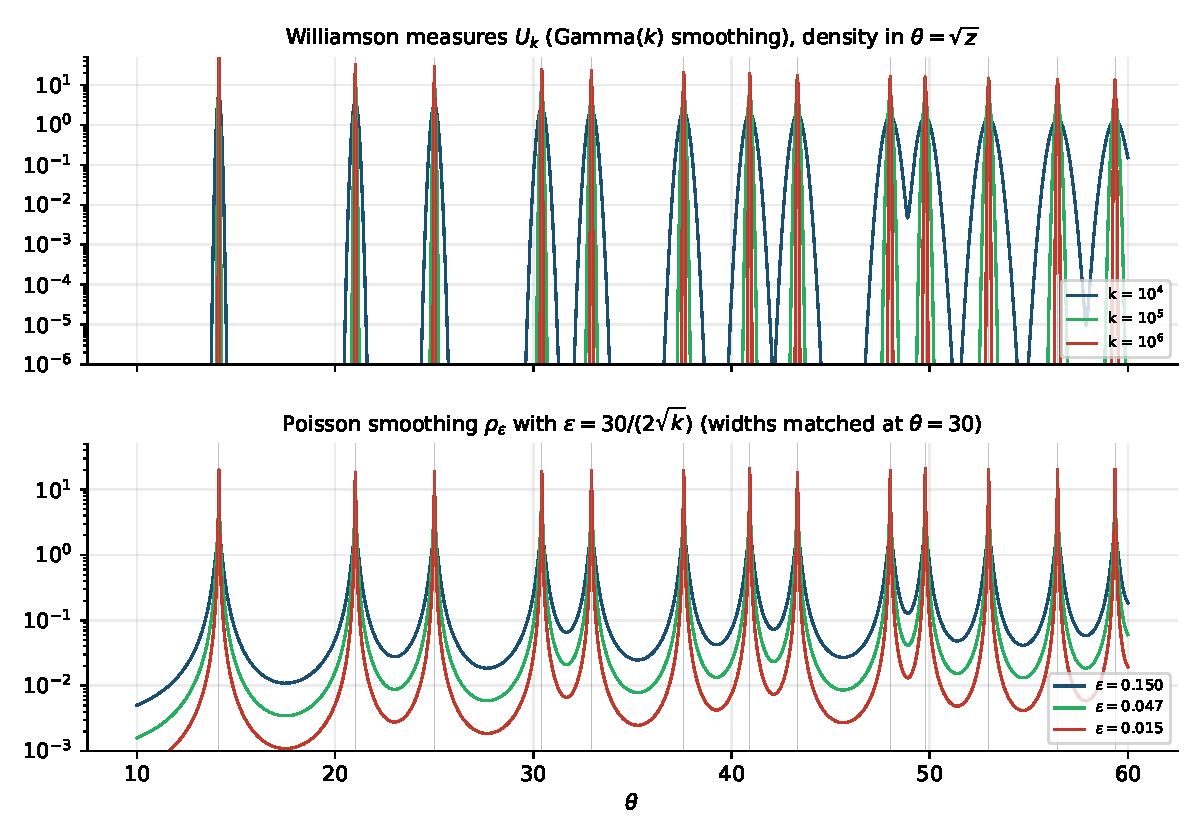
\includegraphics[width=0.95\textwidth]{fig/kmono.pdf}
\caption{Top: the Williamson measures $U_k$ of the heat trace for $k=10^4$, $10^5$, $10^6$, computed from $1700$ zeros, as densities in $\theta=\sqrt z$. Bottom: the Poisson smoothed Thorin densities $\rho_\varepsilon$ with $\varepsilon=30/(2\sqrt k)$, so that the widths match at $\theta=30$.}
\label{fig:ch12:kmono}
\end{figure}

The Poisson smoothing of the zeros is $\pi^{-1}\re(\xi'/\xi)$ off the line and can be computed from $\xi$ alone at every resolution, which is why $\rho_\varepsilon$ is the central object of Chapter~\ref{chap:measure} and Section~\ref{ch:weak}; the price is the heavy tail, which makes positivity at one resolution a statement about all zeros at once. The gamma smoothing is local, and an off line pair contributes to $U_k$ a signed, oscillating term near its height.

\subsection{Along a ray: the Gaussian smoothing of the zeros}\label{sec:ch12:ray}

Fix a height $u$ and move along the ray $t=k/u^2$ of the $(k,t)$ plane, on which the weight $x^ke^{-xt}$ of $c_k(t)$ peaks at $x=u^2$ and the density of $U_k$ is taken at $z=u^2$. Write each zero as $\rho=\frac12+\delta+i\gamma$ and put $\tilde\gamma=\gamma-i\delta$, so that $a=\tilde\gamma^2$; as in every sum of this section, the zero is taken with $\gamma>0$ from each pair $\{\rho,1-\rho\}$. The Gaussian smoothing of the zeros at resolution $1/(2\sqrt t)$ is
\[
\mathcal G(u,t)=\sum e^{-2t(\tilde\gamma-u)^2}.
\]
A zero on the line contributes a Gaussian bump at its ordinate. The zeros $\frac12\pm\delta+i\gamma$ of a quadruple $\frac12\pm\delta\pm i\gamma$ have conjugate values of $\tilde\gamma$, so $\mathcal G$ is real, and together they contribute $2e^{2t(\delta^2-(\gamma-u)^2)}\cos(4t\delta(\gamma-u))$, a bump amplified by $e^{2t\delta^2}$ and modulated in $u$ with period $\pi/(2t\delta)$. At $u=0$, $\mathcal G(0,t)=W(2t)$.

\begin{proposition}\label{prop:ch12:ray}
Let $u\ge2$, $t>0$ and $k=u^2t$, not necessarily an integer, with $a^k$ the principal power in $c_k(t)=\sum a^ke^{-at}$, and let $f_0=k(\log u^2-1)$. Then
\[
e^{-f_0}c_k(t)=\sum_{|\tilde\gamma-u|\le u/2}e^{-2t(\tilde\gamma-u)^2}\big(1+\varepsilon_\rho\big)+R,\qquad |\varepsilon_\rho|\le\exp\Big\{\frac{4t}{3u}|\tilde\gamma-u|^3\Big\}-1,
\]
where, with $\ell_\pm=u\pm\frac12\sqrt{u^2-1}$, $H(r)=u^2\log\frac{r^2+1/4}{u^2}-r^2+\frac14+u^2$ and $\eta=1-u^2/(\ell_+^2+\frac14)>0$,
\[
|R|\le N(\ell_-)e^{tH(\ell_-)}+\Big(\ell_+^2+\frac1{t\eta}\Big)e^{tH(\ell_+)}.
\]
No hypothesis on the zeros is used.
\end{proposition}

\begin{proof}
Put $\tilde\gamma=u+v$ and $w=v/u$. Since $\re\tilde\gamma>0$ and $|\arg\tilde\gamma|<\frac\pi4$, the principal logarithm gives $e^{-f_0}a^ke^{-at}=e^E$ with
\[
E=tu^2\big(2\log(1+w)-2w-w^2\big)=-2tv^2+2tu^2\sum_{m\ge3}\frac{(-1)^{m+1}w^m}m ,
\]
and for $|w|\le\frac12$ the series has modulus at most $|w|^3/(3(1-|w|))\le\frac23|w|^3$. This gives $\varepsilon_\rho=e^{E+2tv^2}-1$ and its bound, since $|e^z-1|\le e^{|z|}-1$. For a zero with $|v|>u/2$, $|v|^2=(\gamma-u)^2+\delta^2$ and $\delta^2<\frac14$ give $|\gamma-u|>\frac12\sqrt{u^2-1}$, so that $\gamma<\ell_-$ or $\gamma>\ell_+$, and $|e^E|=\exp t\big(u^2\log(|a|/u^2)-\re a+u^2\big)\le e^{tH(\gamma)}$, because $|a|=\gamma^2+\delta^2$ and $\re a=\gamma^2-\delta^2$. The function $H$ increases up to $\sqrt{u^2-\frac14}$, which lies between $\ell_-$ and $\ell_+$, so each of the at most $N(\ell_-)$ zeros below $\ell_-$ contributes at most $e^{tH(\ell_-)}$. For $r\ge\ell_+$, $\log(1+x)\le x$ gives $H(r)\le H(\ell_+)-\eta(r^2-\ell_+^2)$. The explicit Riemann von Mangoldt formula \cite[Corollary~1.2]{HSW22} gives $N(r)\le r^2$ for every $r$, and partial summation then gives $\sum_{\gamma>\ell_+}e^{-q(\gamma^2-\ell_+^2)}\le\ell_+^2+1/q$ for $q>0$; take $q=t\eta$.
\end{proof}

For $u\ge10$ the ratios $H(\ell_-)/u^2$ and $H(\ell_+)/u^2$ decrease in $u$, from $-0.616$ and $-0.431$ at $u=10$, and $\eta>0.55$, so that $|R|\le(3u^2+2/t)e^{-0.43k}$. What remains is $\varepsilon_\rho$, whose term of order $1/u$ is $\frac{2t}{3u}(\tilde\gamma-u)^3$. Along the ray, therefore, $e^{-f_0}c_k(t)$ is $\mathcal G(u,t)$ up to an exponentially small remainder and, in each term, a relative error at most $e^{4t|\tilde\gamma-u|^3/3u}-1$. That error is small, of order $t|\tilde\gamma-u|^3/u$, for the terms that carry the sum provided $t|\tilde\gamma-u|^3$ is small against $u$ for them; for the zeros within a few multiples of $1/\sqrt t$ of $u$ it is of order $1/(\sqrt t\,u)$. It is not small in general: at a fixed height, as $t$ grows, the term of the nearest zero dominates, and its relative error grows with $t$. For an integer $k$ the density of $U_k$ in the chart $\theta=\sqrt z$ is exactly $\sqrt{2t/\pi}\,e^{-\lambda_k}e^{-f_0}c_k(t)$ at $\theta=u$, where $t=k/u^2$ and $\lambda_k\in(\frac1{12k+1},\frac1{12k})$ is the remainder in Stirling's formula for $k!$ \cite{Robbins55}. The density of $U_k$ at $\theta$ is therefore about $\sqrt{2t/\pi}\,\mathcal G(\theta,t)$ with $t=k/\theta^2$: the zeros smoothed by normal densities of standard deviation $1/(2\sqrt t)=\theta/(2\sqrt k)$, which is the width found above.

\begin{proposition}\label{prop:ch12:gauss}
RH holds if and only if $\mathcal G(u,t)\ge0$ for every real $u$ and every $t>0$.
\end{proposition}

\begin{proof}
Under RH every term is positive. Suppose that $\frac12+d+ic$ is a zero with $d>0$, and let $|u-c|<\frac d2$. The term of a zero has modulus $e^{2t\phi}$ with $\phi=\delta^2-(\gamma-u)^2$. For the zero $\frac12+d+ic$, $\phi>\frac34d^2$; for a zero with $|\gamma-c|>1$, $\phi<\frac14-\frac9{16}<0$. Group the finitely many zeros with $|\gamma-c|\le1$ by their type $(\gamma,|\delta|)$. Two types at the same ordinate have exponents $\phi$ differing by a nonzero constant, and two at different ordinates have exponents differing by a nonconstant affine function of $u$, so outside finitely many points one type has the largest $\phi$. Fix such a $u_*$, different from every ordinate, and let $(\gamma_*,d_*)$ be the maximising type and $\phi_*$ its exponent. Then $\phi_*>\frac34d^2$, so $d_*>0$, and the type consists of $\nu\ge2$ zeros counted with multiplicity, which contribute $\nu e^{2t\phi_*}\cos(4td_*(\gamma_*-u_*))$. Along $t_j=(2j+1)\pi/(4d_*|\gamma_*-u_*|)$ this is $-\nu e^{2t_j\phi_*}$. The other $n$ zeros with $|\gamma-c|\le1$ contribute at most $ne^{2t_j(\phi_*-\Delta)}$, with $\Delta>0$ the gap to the next exponent, and the zeros with $|\gamma-c|>1$ at most $32\log(c+2)e^{-5t_j/8}$ once $t_j\ge1$, since by the explicit Riemann von Mangoldt formula every interval of heights $[y,y+1]$ holds at most $4\log(y+3)$ zeros. Hence
\[
e^{-2t_j\phi_*}\mathcal G(u_*,t_j)\le-\nu+ne^{-2t_j\Delta}+32\log(c+2)e^{-(2\phi_*+5/8)t_j},
\]
which is negative for all large $j$.
\end{proof}

\begin{proposition}\label{tx:prop:offline}
For $\frac12<\alpha<1$ let $\eta=\alpha-\frac12$ and $\mathcal G_\alpha(u,t)=\re\sum e^{-2t(\tilde\gamma+i\eta-u)^2}$, over the zeros with $\gamma>0$ as for $\mathcal G$, which is $\mathcal G$ at $\eta=0$. Under RH $\mathcal G_\alpha(u,t)<0$ for some $u$ and $t$: there is no Gaussian criterion on the line $\re s=\alpha$.
\end{proposition}

\begin{proof}
Under RH $\tilde\gamma=\gamma$, and the term of $\gamma$ is $e^{2t\eta^2}e^{-2t(\gamma-u)^2}\cos\big(4t\eta(\gamma-u)\big)$. Take $u=\gamma_1+\pi/(4t\eta)$, where $\gamma_1$ is the lowest ordinate and a simple zero, and let $g>0$ be the gap to the next ordinate. The term of $\gamma_1$ is $-e^{2t\eta^2-\pi^2/(8t\eta^2)}$. For $t\ge\pi/(2\eta g)$ every other $\gamma$ has $\gamma-u\ge(\gamma-\gamma_1)/2$, so the other terms total at most $e^{2t\eta^2}\sum_{\gamma>\gamma_1}e^{-t(\gamma-\gamma_1)^2/2}=o(e^{2t\eta^2})$. Hence $\mathcal G_\alpha(u,t)=-e^{2t\eta^2}(1+o(1))<0$ as $t\to\infty$.
\end{proof}

Proposition~\ref{prop:ch12:gauss} restricts Weil's criterion to the modulated Gaussians. For $f(x)=e^{-x^2/4t-iux}$ the transform $\hat f(r)=\int f(x)e^{irx}dx=\sqrt{4\pi t}\,e^{-t(r-u)^2}$ gives, summed over all zeros $\rho=\frac12+i\gamma_\rho$,
\[
\sum_\rho\hat f(\gamma_\rho)\overline{\hat f(\bar\gamma_\rho)}=4\pi t\big(\mathcal G(u,t)+\mathcal G(-u,t)\big),
\]
where $\mathcal G(-u,t)$ comes from the zeros $1-\rho$ and is at most $e^{t/2}((u+14)^2+\frac1{2t})e^{-2t(u+14)^2}$ in modulus for $u\ge0$, too little to change the sign in the proof. At $u=0$ the family gives the first rung, $\mathcal G(0,t)=W(2t)>0$ (Theorem~\ref{thm:ch12:idsd}). Since the Gaussian is entire, Weil's formula of Section~\ref{ch:clock} applies to $h(r)=e^{-2t(r-u)^2}+e^{-2t(r+u)^2}$, for which $\sum_\rho h(\gamma_\rho)=2(\mathcal G(u,t)+\mathcal G(-u,t))$, and gives $\mathcal G$ from the primes:
\begin{equation}\label{eq:ch12:Garith}
\begin{aligned}
\mathcal G(u,t)+\mathcal G(-u,t)&=2e^{t/2-2tu^2}\cos2tu+A(u,t)-P(u,t),\\
A(u,t)&=\frac1{4\pi}\int_{\mathbb R}\big(e^{-2t(r-u)^2}+e^{-2t(r+u)^2}\big)m(r)\,dr,\\
P(u,t)&=\frac1{\sqrt{2\pi t}}\sum_{n\ge2}\frac{\Lambda(n)}{\sqrt n}e^{-(\log n)^2/8t}\cos(u\log n),
\end{aligned}
\end{equation}
with $m$ as in \eqref{eq:ch2:Warith}.

Table~\ref{tab:ch12:gweil} computes both sides. The prime sum converges at every resolution, but more slowly the finer the resolution: since Chebyshev's function $\psi(x)=\sum_{n\le x}\Lambda(n)$ grows like $x$, the weight $n^{-1/2}e^{-(\log n)^2/8t}$ acts, as a density in $\log n$, like $e^{t/2}$ times a Gaussian with centre $2t$ and standard deviation $2\sqrt t$. At $t=3$ (last row) the rest of the prime sum beyond $10^9$ is nearly all main term: with the integral $(2\pi t)^{-1/2}\int_N^\infty x^{-1/2}e^{-(\log x)^2/8t}\cos(u\log x)\,dx$ that the prime number theorem predicts for it, the difference at $N=10^9$ falls to $3\times10^{-10}$. Where $\mathcal G$ is small the two arithmetic terms cancel, the more deeply the finer the resolution, as for $W$ in Table~\ref{tab:ch2:W}; these are the points where an off line quadruple would first make $\mathcal G$ negative (Section~\ref{ch:finite}).

\begin{table}[htbp]
\centering\footnotesize\setlength{\tabcolsep}{2.5pt}
\begin{tabular}{@{}rrllllll@{}}
\toprule
$u$ & $t$ & $\mathcal G(u,t)$ & $A(u,t)$ & $P(u,t)$ & \multicolumn{3}{c}{$|\mathcal G-A+P_N|$}\\
& & & & & $N=10^4$ & $N=10^6$ & $N=10^9$\\
\midrule
$100$ & $1$ & $0.0960845325$ & $0.5519917891$ & $0.4559072567$ & $2.3\times10^{-6}$ & $1.2\times10^{-10}$ & $9.6\times10^{-19}$\\
$1977.22$ & $1.75$ & $1.9835406644$ & $0.8672562847$ & $-1.1162843797$ & $1.2\times10^{-3}$ & $1.3\times10^{-7}$ & $2.2\times10^{-13}$\\
$1000$ & $2$ & $0.8452691893$ & $0.7150931047$ & $-0.1301760846$ & $5.8\times10^{-4}$ & $5.8\times10^{-6}$ & $1.9\times10^{-11}$\\
$100$ & $3$ & $0.0003053958$ & $0.3186935678$ & $0.3183870527$ & $2.0\times10^{-3}$ & $5.4\times10^{-4}$ & $1.1\times10^{-6}$\\
\bottomrule
\end{tabular}
\caption{The Gaussian smoothing of the zeros from the zeros and from the primes, by \eqref{eq:ch12:Garith}. $\mathcal G(u,t)$ is summed over the zeros below height $2197.26$, the rest adding less than $10^{-70000}$; the polar term and $\mathcal G(-u,t)$ are below $10^{-8000}$. $P_N$ is $P$ with the sum cut at $n\le N$, and the $P$ column is $P_{10^9}$. The bound on the rest of the prime sum that ignores its phases, from $\psi(x)<1.03883x$ \cite[Theorem 12]{RS62}, is $1.6\times10^{-20}$, $2.1\times10^{-10}$, $1.0\times10^{-8}$ and $1.0\times10^{-4}$ at $N=10^9$ for the four rows; in the first row the difference at $N=10^9$ is the rounding error of the sums, in extended precision.}
\label{tab:ch12:gweil}
\end{table}

\subsection{What a verification height buys}\label{sec:ch12:reach}

Chapters~\ref{chap:rzeta} and \ref{chap:rzid} reach further rungs by the same method. Adding to the clock variable an independent positive stable variable of index $\frac12$, that is, multiplying the clock by $e^{-c\sqrt u}$ with $c=\zeta'(\frac12)/\zeta(\frac12)=2.6860917$, gives the floor $e^{-c\sqrt u}\,\xi(\frac12)/\xi(\frac12+\sqrt u)$ of Section~\ref{ch:rz2}, whose canonical function, $y$ times its L\'evy density, is $k(y)=W(y)+c/(2\sqrt{\pi y})$. By Theorem~\ref{thm:ch12:idsd}, $k>W>0$, so the floor is infinitely divisible unconditionally; Section~\ref{ch:rz2} proves this independently, and proves that the floor is a GGC if and only if RH holds (Theorem~\ref{rz:thm:floor}). Weil's functional is positive on the cone of test functions completely monotone in $r^2$ (Theorem~\ref{rz:thm:bernsteincone}); this is the first rung integrated against a positive weight, $\sum_\rho\hat h(\gamma_\rho)=2\int_0^\infty W(y)g(y)\,dy$ with $g\ge0$, and for it Section~\ref{ch:rz4} proves $W>0$ afresh.

Every rung is reached by the same mechanism: near the origin the archimedean term dominates the primes, and away from it a known positive term, usually a verified low zero, dominates the unverified high zeros. Only the second limits the order, as the proof of Theorem~\ref{thm:ch12:cm} shows. The first limits the time instead: it gives every order $k\ge1$ up to $t=0.019$, and every order above $10^{17}$ up to $t=1.29$ (Theorem~\ref{thm:ch12:cmint}).

\begin{theorem}\label{thm:ch12:window}
Let $H=3\times10^{12}$, the height to which RH is verified \cite{PT21}. Then $(-1)^kW^{(k)}(t)>0$ for every $t\ge1.29$ and every integer $k$ with $0\le k\le t(H-23)^2$. Consequently $(-1)^kW^{(k)}(t)>0$ for every $t>0$ and every integer $k$ with $0\le k\le1.29(H-23)^2$, and $1.29(H-23)^2>1.16\times10^{25}$.
\end{theorem}

\begin{proof}
Fix $t\ge1.29$ and $k$, and put $u=\sqrt{k/t}$, $D=H-u\ge23$ and $f(v)=v^{2k}e^{-tv^2}$. As in Section~\ref{sec:ch12:ray}, write each zero as $\frac12+\delta+i\gamma$ and put $\tilde\gamma=\gamma-i\delta$, so that $c_k(t)=\sum f(\tilde\gamma)$ over one zero of each pair $\{\rho,1-\rho\}$, taken with $\gamma>0$. On $(0,\infty)$, $(\log f)''=-2k/v^2-2t$ is at most $-2t$, and at least $-4t$ on $[u,\infty)$, while $(\log f)'(u)=0$; hence $f(v)\le f(u)e^{-t(v-u)^2}$ for every $v>0$, and $f(v)\ge f(u)e^{-2t(v-u)^2}$ for $v\ge u$. The zeros below height $H$ lie on the line and contribute $f(\gamma)>0$. One of them lies in $[u,u+15]$: for $u\le1000$ because $\gamma_1<15$ and consecutive ordinates below $1015$ differ by less than $7$, and for $u\ge1000$ because the explicit Riemann von Mangoldt formula of \cite[(1.7) and Corollary~1.4]{HSW22} gives $N(u+15)-N(u)>4$. That zero contributes at least $f(u)e^{-450t}$. A zero above $H$, wherever it lies, has $|\delta|<\frac12$ and $|\tilde\gamma|\ge\gamma>u$, so its term has modulus $f(|\tilde\gamma|)e^{2t\delta^2}\le e^{t/2}f(u)e^{-t(\gamma-u)^2}$. Partial summation with $N(r)\le r^2$, and $\int_D^\infty e^{-tv^2}dv\le e^{-tD^2}/(2tD)$, give
\[
\sum_{\gamma>H}e^{-t(\gamma-u)^2}\le e^{-tD^2}\Big(H^2+\frac1t+\frac H{tD}\Big),
\]
and therefore
\[
\frac{c_k(t)}{f(u)}\ge e^{-450t}-e^{t/2-tD^2}\Big(H^2+\frac1t+\frac H{tD}\Big)>0,
\]
since $t(D^2-450.5)\ge1.29\cdot78.5>101$ while $\log(H^2+1+H/23)<57.5$. For the second statement, Theorem~\ref{thm:ch12:cmint}(b) gives every order for $t\le1.29$, and for $t>1.29$ every $k\le1.29(H-23)^2$ satisfies $k\le t(H-23)^2$. The program \texttt{window\_orders.py} (\texttt{code/\allowbreak README.md}) computes the zeros below height $1015$ in ball arithmetic and evaluates every numerical inequality of the proof.
\end{proof}

For the floor, $c/(2\sqrt{\pi y})$ is completely monotone, so Theorem~\ref{thm:ch12:window} gives $(-1)^nk^{(n)}>0$ for every $n\le1.16\times10^{25}$; Theorem~\ref{rz:thm:nmono} proves $n\le10^{10}$ independently, with a Cauchy circle of radius $y/2$, which loses a factor $2^n$ and makes its reach grow only linearly in $H$.

\subsection{A compound Poisson defect of the off line zeros}\label{sec:xg:defect}

Group the exponents $a_k$ into the real ones, $a_k=\gamma^2>0$, which belong to zeros on the line, and the conjugate pairs $\{a,\bar a\}$ of nonreal exponents, one for each off line quadruple $\frac12\pm\delta\pm i\gamma$, for which $a=A-iB$ with $A=\gamma^2-\delta^2$ and $B=2\delta\gamma$. Each pair contributes $2e^{-At}\cos(Bt)$ to $W$, and $\cos\theta=1-2\sin^2(\theta/2)$ splits this into a Laplace transform part and a nonnegative remainder.

\begin{theorem}\label{xg:thm:defect}
Unconditionally, $W(t)=\int_{(0,\infty)}e^{-tz}\,U_+(dz)-R(t)$, where $U_+$ is a Thorin measure, $R\ge0$, and
\[
U_+=\sum_{a_k\text{ real}}\delta_{a_k}+2\sum_{\text{pairs}}\delta_A,\qquad R(t)=4\sum_{\text{pairs}}e^{-At}\sin^2\!\Big(\frac{Bt}2\Big).
\]
Let $T_+$ be the GGC with Thorin measure $U_+$, and $Y$ the infinitely divisible variable with L\'evy density $R(t)/t$, independent of $T$. Then
\[
T+Y\stackrel d=T_+,\qquad \E e^{-uY}=\prod_{\text{pairs}}\frac{(1+u/a)(1+u/\bar a)}{(1+u/A)^2}.
\]
The defect $Y$ is compound Poisson, with rate and jump density
\[
\lambda=\int_0^\infty\frac{R(t)}t\,dt=\sum_{\text{pairs}}\log\Big(1+\frac{B^2}{A^2}\Big),\qquad\frac{R(t)}{\lambda t},
\]
and $\lambda<10^{-12}$, so $\Pr(Y=0)=e^{-\lambda}>1-10^{-12}$. The following are equivalent: $R\equiv0$; $Y=0$; RH. In that case $U_+=U_{\RH}$ and $T_+=T$.
\end{theorem}

\begin{proof}
The decomposition is the identity applied pair by pair, and $U_+$ is a Thorin measure because $A\ge\frac12|a|$, since $|a|=\gamma^2+\delta^2$ and $\gamma>14$, and $\sum_k|a_k|^{-1}<\infty$. By Tonelli and the Frullani type integral $\int_0^\infty e^{-At}\sin^2(Bt/2)\,t^{-1}dt=\frac14\log(1+B^2/A^2)$, the function $R(t)/t$ is integrable on $(0,\infty)$ with integral $\lambda$, which is finite by the bound below, and a L\'evy measure of finite mass is compound Poisson. For the bound let $H=3\times10^{12}$. Every pair has $\gamma>H$, and $\delta<\frac12$ gives $B^2/A^2=4\delta^2\gamma^2/(\gamma^2-\delta^2)^2<\gamma^2/(\gamma^2-\frac14)^2<(1+10^{-24})\gamma^{-2}$. The two zeros $\frac12\pm\delta+i\gamma$ of a pair have the same ordinate, so $\lambda<\frac12(1+10^{-24})\sum_{\gamma>H}\gamma^{-2}$, the sum running over all zeros of ordinate above $H$. Partial summation with the explicit bound for $N(T)$ of \cite[Corollary~1.2]{HSW22}, exactly as for $\varepsilon_H$ in the proof of Proposition~\ref{mw:prop:approx}, gives $\sum_{\gamma>H}\gamma^{-2}<1.4798\times10^{-12}$, hence $\lambda<7.4\times10^{-13}$. The program \texttt{xg\_defect.py} (\texttt{code/\allowbreak README.md}) evaluates this bound in ball arithmetic.

By the formula for $\log G$ at the start of this section and Frullani's integral $\log(1+u/z)=\int_0^\infty(1-e^{-ut})e^{-zt}t^{-1}dt$,
\[
\log G(u)=\int_0^\infty\big(1-e^{-ut}\big)\frac{W(t)}t\,dt=\int\log\Big(1+\frac uz\Big)U_+(dz)-\int_0^\infty\big(1-e^{-ut}\big)\frac{R(t)}t\,dt,
\]
that is, $\E e^{-uT}\,\E e^{-uY}=\E e^{-uT_+}$, and the product formula follows from $\E e^{-uT_+}=\prod_{a_k\text{ real}}(1+u/a_k)^{-1}\prod_{\text{pairs}}(1+u/A)^{-2}$ and \eqref{eq:ch2:hadamard}. For the equivalences: every term of $R$ is nonnegative, and a pair contributes a positive term outside the discrete set $\{t>0:Bt\in2\pi\mathbb Z\}$, so $R\equiv0$ if and only if there is no pair, that is, every $a_k$ is real, which happens only for zeros on the line; and $Y=0$ if and only if $\lambda=0$ if and only if $R\equiv0$. Under RH, $U_+=\sum_k\delta_{a_k}=U_{\RH}$ and $T_+=T$ by Proposition~\ref{prop:rigid}.
\end{proof}

\begin{remark}\label{xg:rem:defect}
Unconditionally, therefore, the clock plus an independent compound Poisson variable of rate below $10^{-12}$ is a GGC, and the law of the clock is within total variation $10^{-12}$ of that GGC, since $T=T+Y$ on the event $\{Y=0\}$.
\end{remark}

\subsection{The prime side of the ladder}\label{sec:ps:ladder}

The proofs of Theorems~\ref{thm:ch12:cmint} and \ref{thm:ch12:window} stop at $1.29$ and $1.16\times10^{25}$ because of the constant $K=10^{17}$ with which the proof of Theorem~\ref{thm:ch12:cmint} uses Lemma~\ref{lem:ch12:hermite}(b): as the discussion after Theorem~\ref{thm:ch12:cmint} says, $1.2912$ is the root of $E_{K+1}(t)=2S(t)$ for that $K$. Theorem~\ref{thm:ch12:window} supplies every order up to $1.16\times10^{25}$, and the lemma can be used with that order in the place of $10^{17}$. The root of $E_{K+1}(t)=2S(t)$ then moves to about $1.719$ in floating point, and the argument of both theorems runs at $t=1.70$.

\begin{theorem}\label{ps:thm:free}
$W$ is completely monotone on $(0,1.70]$, and $(-1)^kW^{(k)}(t)>0$ for every $t>0$ and every integer $k$ with $0\le k\le1.70(H-23)^2$, where $H=3\times10^{12}$; and $1.70(H-23)^2>1.52\times10^{25}$.
\end{theorem}

\begin{proof}
Let $K=1.16\times10^{25}$. By Theorem~\ref{thm:ch12:window}, $(-1)^kW^{(k)}(t)>0$ for every $t>0$ and every $k\le K$. For $k>K$ and $t\le0.019$, Theorem~\ref{thm:ch12:cmint}(a) applies. For $k>K$ and $t\in[0.019,1.70]$ the proof of Theorem~\ref{thm:ch12:cmint}(b) applies with $K$ in the place of $10^{17}$ and $1.70$ in the place of $1.29$, and with the cutoff $n_0=10^9$ in the place of $2^{24}$: Lemma~\ref{lem:ch12:hermite}(b) with $\varepsilon=10^{-6}$ gives $C_\varepsilon(k)\le C_\varepsilon(K+1)<1+6\times10^{-7}$ for $k>K$, and the condition $e^2x^2\le4\varepsilon k$ holds for $x\le2\sqrt{\varepsilon(K+1)}/e$, which exceeds $2.5\times10^9$, which covers every prime power $n\le10^9$ at $t\ge0.019$ (there $x_n<76$). The monotonicity in $k$ and $t$ is that of the proof, so it suffices to show $E_{K+1}(1.70)-S_C(1.70)-Q_{K+1}(1.70)>0$, with $S_C$ the sum $S_B$ with $B(x_n)$ replaced by $C$ for $n\le10^9$. Chernoff's bound for the gamma law with $a=(1-2^{-13})^2\lambda$ gives $E_{K+1}(1.70)>26.7532$; the prime powers $n\le10^9$ give $S_C(1.70)<26.2968$, with the tail bound of that proof, which is $2.9\times10^{-4}$ at $q=\log n_0/8t=1.52$; and $Q_{K+1}(1.70)<e^{-1000}$. The margin exceeds $0.4564$. So the orders $k>K$ have the right signs on $(0,1.70]$ and, with the orders $k\le K$, $W$ is completely monotone there.

For $t>1.70$ and $k\le1.70(H-23)^2$ the proof of Theorem~\ref{thm:ch12:window} applies with $1.70$ in the place of $1.29$, since $k\le t(H-23)^2$ and the only place where the lower bound on $t$ enters is $t(D^2-450.5)\ge1.70\cdot78.5>133$, against $\log(H^2+1+H/23)<57.5$. Finally $1.70(H-23)^2>1.52\times10^{25}$. The program \texttt{cm\_orders\_k116e25.py} (\texttt{code/\allowbreak README.md}) evaluates every numerical inequality of the argument for $k>K$ in ball arithmetic, with the prime powers $n\le10^9$ ($50\,851\,223$ of them): all of them hold.
\end{proof}

In floating point the root of $E_{K+1}(t)=2S(t)$ for $K=1.52\times10^{25}$ is about $1.724$, which is the time $t_0=1.72$ of the phase free bound at the verified height (Section~\ref{ch:lessons}); $1.70$ is the safe round number.

By Proposition~\ref{prop:ch12:ray}, on the ray $t=k/u^2$ the rung is, up to the errors of that proposition, $\mathcal G(u,t)$, and \eqref{eq:ch12:Garith} writes $\mathcal G(u,t)+\mathcal G(-u,t)$ as a polar term plus $A(u,t)-P(u,t)$, where $A(u,t)$ is close to $\log(u/2\pi)/(2\sqrt{2\pi t})$ and $P(u,t)=(2\pi t)^{-1/2}\Pi(u;t)$, with $\Pi(T;x)=\sum_{n\ge2}\Lambda(n)n^{-1/2}e^{-(\log n)^2/8x}\cos(T\log n)$ the smoothed prime sum. To leading order, therefore, the rung at height $T$ and scale $x$ is positive when $2\Pi(T;x)<\log(T/2\pi)$, and this is the comparison of the archimedean term with the prime term for which Section~\ref{ch:lessons} gives the phase free time $t_0(T)$, which agrees to five digits with $x_c(T)$, the root of $M(x)=\log(T/2\pi)$ with $M(x)=2\sum_{n\ge2}\Lambda(n)n^{-1/2}e^{-(\log n)^2/8x}$ (twice the sum $S(x)$ of that section). Below $x_c(T)$ it holds whatever the phases are; above it, it is a statement about cancellation among the primes, which Proposition~\ref{prop:ch12:gauss} makes an exact criterion for RH, with $A$ and $\mathcal G$ in place of the leading terms.

The comparison can be evaluated at heights far beyond verification, because the cost depends on $T$ only through the precision of $T\log n$ modulo $2\pi$. The table gives $2\Pi(T;x)$ against $\log(T/2\pi)$, with the prime powers $n\le N$, $N=\lfloor e^{\sqrt{8xD}}\rfloor$ for the tolerance $D=22$ at $x\le1$, $D=20$ at $x=1.7$, $D=16$ at $x=2.5$ and $D=14$ at $x=3$, and the phases in ball arithmetic at $300$ bits. The weight of the omitted prime powers is about $e^{\sqrt{2xD}-D}$ times a factor of order one, not $e^{-D}$; the Prime Number Theorem estimate of the sum of their absolute values is below $1.5\times10^{-2}$ in every row. The values are not certified, and the leading term $\log(T/2\pi)$ stands for the archimedean term $A(T,x)$, with a relative error $O(T^{-2})$. The condition holds in every row; the scales $x=1.7$, $2.5$ and $3$ at $T=10^{12}$ are above $x_c(10^{12})=1.679$ (computed), where the weights alone no longer decide.

\begin{center}
\small\setlength{\tabcolsep}{4pt}
\begin{tabular}{rrrrrr}
\toprule
$T$ & $x$ & $N$ & $2\Pi(T;x)$ & $\log(T/2\pi)$ & $\pi/(4x)$\\
\midrule
$10^{12}$ & $0.5$ & $1.2\times10^4$ & $-0.187$ & $25.79$ & $1.57$\\
$10^{12}$ & $1.0$ & $5.8\times10^5$ & $-0.374$ & $25.79$ & $0.79$\\
$10^{12}$ & $1.7$ & $1.5\times10^7$ & $-0.142$ & $25.79$ & $0.46$\\
$10^{12}$ & $2.5$ & $5.9\times10^7$ & $0.630$ & $25.79$ & $0.31$\\
$10^{12}$ & $3.0$ & $9.1\times10^7$ & $1.279$ & $25.79$ & $0.26$\\
$3\times10^{12}$ & $1.7$ & $1.5\times10^7$ & $-0.266$ & $26.89$ & $0.46$\\
$3\times10^{12}$ & $3.0$ & $9.1\times10^7$ & $-2.713$ & $26.89$ & $0.26$\\
$10^{20}$ & $1.0$ & $5.8\times10^5$ & $-0.720$ & $44.21$ & $0.79$\\
$10^{30}$ & $1.0$ & $5.8\times10^5$ & $-0.077$ & $67.24$ & $0.79$\\
$10^{50}$ & $1.0$ & $5.8\times10^5$ & $0.881$ & $113.29$ & $0.79$\\
\bottomrule
\end{tabular}
\end{center}

The last column is the product $\delta\Delta$ of the displacement and the gap of an isolated off line pair at which, in the local model of Proposition~\ref{xg:prop:local} and to leading order only, a failure of the comparison at the scale $x$ would first be visible, since $t^*_{\rm loc}=\omega^*/(2\delta\Delta)$ with $\omega^*$ just above $\pi/2$ (Section~\ref{sec:xg:local}). The failure sits at one offset of the window in the height, so one value of $T$ excludes nothing and a scan in $T$ over about $\Delta$ is needed. In this reading the prime side resolves only zeros that are well off the line and isolated, and a pair with $\delta\Delta\ll1$, such as a Lehmer type near miss, needs a scale $x\gg1$ at which the cutoff $N$ is out of reach. The program \texttt{prime\_side\_check.py} (\texttt{code/\allowbreak README.md}) computes the table and the values of $M$ and $x_c$ quoted above.

\section{What finite information cannot decide}\label{ch:finite}

Every computation in this book is finite: a finite window, finitely many resolutions, finitely many derivatives or matrix blocks. Theorem~\ref{thm:ch13:perturb} replaces two close zeros of $\xi$ on the line by a quadruple off it \cite[Chapter 11]{P26} and obtains an entire function whose heat trace passes the finite tests of Section~\ref{ch:heat}. Below height $2000$ the order at which its derivative signs first fail can be computed, and it grows roughly like the square of the height. Section~\ref{sec:ch13:visibility} records what each finite test of the book establishes and what it cannot exclude; the sharpest case is positivity of $\rho_\varepsilon$ at one resolution, which can miss zeros far from the line. Finally, a finite computation can refute a sufficient condition for RH: one certified zero of an explicit function closes the Bernstein Pick route through the moments of the P\'olya density.

\subsection{A perturbation that passes the finite tests of the heat trace}\label{sec:ch13:perturb}

\begin{theorem}[{\cite[Theorem D]{P17}}]\label{thm:ch13:perturb}
\textup{(a)} There are ordinates $1000<A<B\le2000$ of zeros on the critical line, with $B-A\le2$, such that, with $g=(A+B)/2$ and $w=\frac14+ig$,
\[
F(s)=\frac{\xi(\frac12+s)}{\xi(\frac12)}\,\frac{(1-s^2/w^2)(1-s^2/\bar w^2)}{(1+s^2/A^2)(1+s^2/B^2)}
\]
is an even entire function with the order, type and reflection symmetry of $\xi(\frac12+s)$ and with four zeros off the critical line, and the following hold. The reciprocal clock $1/F(\sqrt u)$ is the Laplace transform of an infinitely divisible, self decomposable law, and its heat trace
\[
W_F(t)=W(t)+2\re e^{-at}-e^{-A^2t}-e^{-B^2t},\qquad a=-w^2=g^2-\tfrac1{16}-\tfrac{ig}2,
\]
which is $t$ times its L\'evy density, is strictly log convex. $W_F$ has the same small time expansion as $W$ through the constant term, and $1/F$ has the same nearest poles as the reciprocal Xi function.

\textup{(b)} Let $N\ge1$ and $R\ge T_N$, where $T_N=20000N\sqrt{1+\log N}$ as in Section~\ref{ch:heat}, and suppose that every zero of $\xi$ with ordinate in $(0,R+50]$ lies on the critical line. Then the pair can instead be chosen with $R<A\le B\le R+50$ and $B-A<2$ (if $A=B$, a multiple zero supplies both), so that $F$ keeps every property listed in (a) and the leading $N\times N$ Hankel blocks of $W_F$ remain positive definite at every $t>0$. If moreover $R\ge10^{12}$, the derivative signs of Theorem~\ref{thm:ch12:cm} are also preserved: $(-1)^kW_F^{(k)}(t)>0$ for every $t>0$ and every integer $0\le k\le10^{17}$. For every $N\le3\times10^7$ the verification to height $3\times10^{12}$ \cite{PT21} establishes the hypothesis on the zeros for $R=\max(T_N,10^{12})$, so that such an $F$ with both properties exists unconditionally.
\end{theorem}

The construction moves the zeros at heights $A$ and $B$, with their conjugates, to the quadruple $\frac12\pm\frac14\pm ig$. The heat trace changes by the oscillating term $W_F-W$, whose envelope is bounded as in Section~\ref{ch:heat} \cite[Proposition 11.1]{P17}, and at the heights of (b) this change is smaller than the margin by which each of its tests holds. The pair of (b), with the properties of (a) and the Hankel blocks, comes from \cite[Theorem 12.5]{P17}, the derivative signs from \cite[Proposition 12.7]{P17}, which holds for any pair of zeros on the line with $A>10^{12}$ and $B-A\le2$, and the unconditional range from \cite[Corollary 12.6]{P17}, since $T_{3\times10^7}+50<2.6\times10^{12}$. Figure~\ref{fig:ch13:perturb} shows the change for a pair in the range of (a), far below the heights that (b) requires; the pair it moves, near height $1977.22$, is the closest pair among the first $1700$ zeros, whether or not the spacings are normalised (Section~\ref{sec:ch15:spacings}).

\begin{figure}[htbp]
\centering
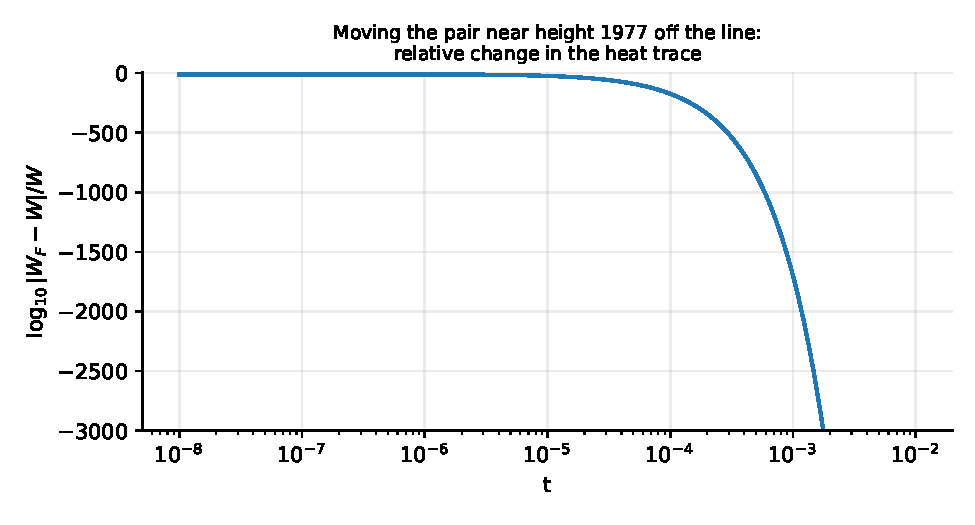
\includegraphics[width=0.72\textwidth]{fig/perturb.pdf}
\caption{Relative change $|W_F-W|/W$ of the heat trace, on a $\log_{10}$ scale, when the closest pair of zeros between heights $1000$ and $2000$ (near $1977.22$) is moved to distance $\frac14$ from the line, computed in forty digit arithmetic with $W$ replaced by its sum over the first $1700$ zeros. The change is at most $4\times10^{-11}$, near $t=7\times10^{-7}$, and falls below $10^{-1000}$ by $t=10^{-3}$. The sum over $1700$ zeros is smaller than $W$, by $1.3$ per cent at $t=7\times10^{-7}$ and by a factor of $5.4$ at $t=10^{-8}$, so the curve bounds the relative change from above; with $W$ from the explicit formula \eqref{eq:ch2:Warith} the maximum is $3.66\times10^{-11}$, at $t=7.2\times10^{-7}$.}
\label{fig:ch13:perturb}
\end{figure}

Not every finite test is passed. Below any height $T>B$ the argument count of $F$ equals that of $\xi$, since $F$ loses the zeros at heights $A$ and $B$ and gains two at height $g$, but these two are off the line, so $F$ has two zeros fewer on the line, counted with multiplicity; when $A<B$ and both zeros are simple, as for the pair of Figure~\ref{fig:ch13:perturb}, it has two sign changes fewer. Turing's comparison of the two counts, the first test of Table~\ref{tab:ch13:see}, then detects the perturbation once it passes height $B$, and the zero density identity at any height $T>g$ returns $\nu(\frac12+\varepsilon,T)\ge1$ for every $\varepsilon<\frac14$, whatever the multiplicities. Counting tests are local in height and find the perturbation once their window contains it, whereas a given finite set of heat trace tests, which involve all the zeros at once, misses it when it lies high enough.

The pair of Figure~\ref{fig:ch13:perturb} lies far below the heights of (b), and at its height the derivative signs of $F$ do fail at a finite order, which can be computed. On the ray $t=k/u^2$ the normalised value $e^{-f_0}c_k^F(t)$ of Proposition~\ref{prop:ch12:ray}, whose proof applies to $F$ because $F$ has at most one zero more than $\xi$ below any height, is a sum of positive terms, one for each zero on the line, the oscillating term of the quadruple and terms, negligible here, from any zeros off the line above $3\times10^{12}$, and only the zeros within a few units of $u$ matter. A scan over $u$ and over the orders, at every order up to $500$, then on a grid of ratio $1.002$ and at every order of the last grid interval, finds that the first order at which $c_k^F(t)<0$ for some $t>0$ is $k=6\,683\,655$, at $t=1.7113393$. The grid loses nothing, because $c_{k-1}^F(t)=\int_t^\infty c_k^F(s)\,ds$: if $c_k^F\ge0$ on $(0,\infty)$ then so is $c_{k-1}^F$, and the orders that fail are all those from the first one on. The negative value is certified in ball arithmetic, with explicit bounds for the zeros below $g-40$, which lie on the line, and for those above $g+40$, wherever the ones above $3\times10^{12}$ lie; the positivity at the lower orders is computed, not certified. Table~\ref{tab:ch13:first} repeats the computation for the closest pair of consecutive zeros in five other windows of height, and for the pair near $1977.22$ moved to distance $0.1$ instead of $\frac14$.

\begin{table}[htbp]
\centering\small\setlength{\tabcolsep}{4pt}
\begin{tabular}{rrrrrrr}
\toprule
window & zeros moved & $g$ & $\delta$ & $k^*$ & $t^*$ & $c_{k^*}^F(t^*)$, normalised\\
\midrule
$(100,200)$ & $71$, $72$ & $185.24$ & $\frac14$ & $40\,018$ & $1.18413$ & $-6.37\times10^{-7}$\\
$(200,400)$ & $186$, $187$ & $376.08$ & $\frac14$ & $219\,169$ & $1.54072$ & $-6.70\times10^{-8}$\\
$(400,700)$ & $363$, $364$ & $630.64$ & $\frac14$ & $624\,921$ & $1.576635$ & $-1.68\times10^{-7}$\\
$(700,1000)$ & $453$, $454$ & $750.81$ & $\frac14$ & $792\,746$ & $1.410725$ & $-9.26\times10^{-8}$\\
$(1000,1500)$ & $922$, $923$ & $1329.12$ & $\frac14$ & $4\,433\,220$ & $2.5121193$ & $-3.37\times10^{-8}$\\
$(1500,2000)$ & $1496$, $1497$ & $1977.22$ & $\frac14$ & $6\,683\,655$ & $1.7113393$ & $-7.12\times10^{-9}$\\
$(1500,2000)$ & $1496$, $1497$ & $1977.22$ & $0.1$ & $15\,722\,219$ & $4.0257254$ & $-6.71\times10^{-11}$\\
\bottomrule
\end{tabular}
\caption{The first failing order of the derivative signs when the closest pair of consecutive zeros in a window of height is moved to the quadruple $\frac12\pm\delta\pm ig$, $g$ the midpoint of the pair. $k^*$ is the least order at which $c_k^F(t)<0$ for some $t>0$, found by a scan of every order up to $500$, a grid of ratio $1.002$ above it and every order of the last grid interval (computed, not certified); $c_{k^*}^F(t^*)<0$ is certified in ball arithmetic. The last column is $c_{k^*}^F(t^*)$ divided by $(k^*/t^*)^{k^*}e^{-k^*}$, the value at $x=k^*/t^*$ of the weight $x^{k^*}e^{-xt^*}$.}
\label{tab:ch13:first}
\end{table}

The first failing order is $k^*=t^*u_*^2$, where $u_*=\sqrt{k^*/t^*}$ is the height of the failure, between $0.69$ and $1.40$ from $g$, so that $k^*$ is within $1.6$ per cent of $t^*g^2$, with $t^*$ between $1.18$ and $2.51$ for $\delta=\frac14$: it grows roughly with the square of the height, while $t^*$ shows no trend in the height on this range. Proposition~\ref{prop:ch12:ray} explains this. Along the ray, $e^{-f_0}c_k^F(t)$ is, up to relative errors of order $t|\tilde\gamma-u|^3/u$ in the terms near $u$, small at these heights and times (Section~\ref{sec:ch12:ray}), the Gaussian smoothing $\mathcal G(u,t)$ of the zeros of $F$, in which the quadruple contributes $2e^{2t(\delta^2-(g-u)^2)}\cos(4t\delta(g-u))$. This term is negative only where $4t\delta|g-u|$ lies in $(\frac\pi2,\frac{3\pi}2)$ modulo $2\pi$, hence at distance at least $\pi/(8t\delta)$ from $g$, where its modulus is at most $2e^{2t\delta^2-\pi^2/(32t\delta^2)}$, while a zero on the line at distance $d$ from $u$ contributes $e^{-2td^2}$. So $\mathcal G(u,t)<0$ requires every zero on the line to lie at a distance $d$ from $u$ with $2td^2>\pi^2/(32t\delta^2)-2t\delta^2-\log2$: for $\delta=\frac14$ that is $d>1.43$ at $t=1$ and $d>0.62$ at $t=2$. The first failure time is therefore set by $\delta$ and by the gaps between the line zeros near the moved pair, which its removal widens; the mean spacing $2\pi/\log(g/2\pi)$ falls from $1.86$ to $1.09$ between the first and last rows, but the gaps near the moved pairs vary more, which is why $t^*$ shows no trend. The first $t$ at which $\min_{|u-g|\le8}\mathcal G(u,t)<0$, computed in floating point, predicts $k^*$ to $0.21$ per cent at height $185$ and to $0.08$ per cent or better at the other heights, and the minimum lies just beyond the distance $\pi/(8t\delta)$ at which the first negative lobe begins, between $0.7$ and $1.4$ from $g$. These failure times of $\mathcal G$ within $8$ of $g$ are certified in ball arithmetic, with the zeros from Arb, for all seven rows of Table~\ref{tab:ch13:first}: $\mathcal G(u,t)>0$ at every centre $u$ within $8$ of $g$ for every $t$ up to the failure time rounded down to two decimals, and $\mathcal G<0$ at one centre at the failure time rounded up to four decimals. For the pair near $1977.22$ that is $\mathcal G>0$ within $8$ of $g$ for every $t\le1.71$ and $\mathcal G(g-0.98587,1.7112)<0$. Far from $g$ the bracket says nothing: near or above $3\times10^{12}$, zeros off the line could make $\mathcal G$ negative earlier. One time suffices for the first statement, since $\sqrt{2t/\pi}\,\mathcal G(\cdot,t)$ at a smaller $t$ is its value at a larger one convolved with a centred normal density: the sum over the zeros below $3\times10^{12}$ is positive on the whole line at $t=1.71$, by an interval cover within $8$ of $g$ and by domination beyond, so it has a uniform positive lower bound at every smaller $t$ within $8$ of $g$, and the zeros above $3\times10^{12}$, wherever they lie, can lower $\mathcal G$ there by less than $10^{-2\times10^{12}}$ (\texttt{gsmooth\_arb.py}); what they add may be large. Unlike the Hankel condition of Theorem~\ref{thm:ch12:hankel} at one time, positivity of $\mathcal G$ at one resolution does not decide whether the zeros are on the line. Moving the pair near $1977.22$ to distance $0.1$ raises $t^*$ from $1.71$ to $4.03$: the closer the quadruple to the line, the finer the resolution needed to see it.

The same mechanism puts the first failure for a quadruple just above the verified height far beyond the orders of (b). There $g^2\approx10^{25}$, so the first failing order is about $10^{25}t^*$, and $t^*$ depends on the gaps around the quadruple, which a computation at height $3\times10^{12}$ would have to supply. The mean spacing there is $0.23$, and for $\delta=\frac14$ a failure at $t\le1$ would need a stretch of length $2.9$, about twelve mean spacings, free of zeros on the line other than the moved pair. A model with the line zeros spread at their mean density gives $t^*\approx10$ there, but the same model gives $5.9$ at height $1977$ against the computed $1.71$, because it ignores the gaps, so it gives the order of magnitude only. Theorem~\ref{thm:ch12:window} certifies the signs of $\xi$ to every order up to $1.29(H-23)^2>1.16\times10^{25}$, with $H=3\times10^{12}$, so a quadruple of $\xi$ just above $H$ could make a sign fail only at a time $t^*>1.29$, at an order of about $t^*H^2$: the orders certified at the time $t^*$ reach that size, and by the model the orders certified at every time fall short of it by a factor of about eight. This is the entry of Table~\ref{tab:ch13:see} on derivative signs.

\subsection{What finite tests establish, and the local visibility condition}\label{sec:ch13:visibility}

Table~\ref{tab:ch13:see} lists, for each finite test used in this book, where it is made, what it establishes and what it cannot exclude. Each entry of the middle column, made rigorous, is an unconditional theorem on its window; the right column is the reason why no accumulation of such entries proves RH.

\begin{table}[htbp]
\centering\small
\begin{tabular}{p{0.27\textwidth}p{0.33\textwidth}p{0.3\textwidth}}
\toprule
test & establishes & cannot rule out\\
\midrule
sign changes and argument count to height $T$ (Sections~\ref{ch:polya} and \ref{ch:classical}) & all zeros below $T$ on the line & anything above $T$\\
$\rho_\varepsilon\ge0$ on $0<\theta\le\Theta$ (Section~\ref{ch:motivation}) & no zero in the window at distance $d>\varepsilon$ from the line with $2/d^2>\sum_j\delta_j^{-2}$ (to first order in $\varepsilon$) & zeros within $\varepsilon$ of the line; zeros farther from it than about $0.78$ of the mean spacing at their height; zeros above the window\\
zero density scan at $T$ (Section~\ref{ch:turing}) & $\nu(\frac12+\varepsilon,T)=0$ for the $\varepsilon$ computed & zeros within $\varepsilon$ of the line; zeros above $T$\\
Hankel blocks of size $N$ (Section~\ref{ch:heat}) & Weil positivity on a finite space & off line zeros above $T_N$\\
derivative signs to order $K$ (Section~\ref{ch:heat}) & finite order Williamson positivity & off line zeros above a height of about $\sqrt{K/1.29}$\\
HCM derivative signs (Section~\ref{ch:weak}) & finitely many CM conditions & failure at other $u$ or orders\\
matched total variation at resolution $\varepsilon$ (Section~\ref{ch:distances}) & agreement with the Poisson smoothing of the list & zeros outside the window\\
Li coefficients $\lambda_n$, $n\le N$ (Section~\ref{ch:li}) & finitely many of Li's inequalities & off line zeros $\frac12\pm d+i\gamma$ with $Nd/\gamma^2$ small\\
\bottomrule
\end{tabular}
\caption{What finite tests establish and what they cannot exclude.}
\label{tab:ch13:see}
\end{table}

The second row rests on a local computation. Suppose that $\xi$ has a pair of zeros $\frac12\pm d+i\gamma$ with $d>\varepsilon$, where $d$ is the displacement written $\delta$ in Section~\ref{ch:heat} and in Proposition~\ref{prop:struct}, and that the other zeros near height $\gamma$ lie on the line at the ordinates $\gamma+\delta_j$. A zero $\rho$ contributes $\re(s-\rho)^{-1}$ to $\pi\rho_\varepsilon(\theta)$, where $s=\frac12+\varepsilon+i\theta$, so at the ordinate, ignoring distant zeros and those at negative heights,
\[
\pi\rho_\varepsilon(\gamma)=\varepsilon\Big(\sum_j\frac1{\delta_j^2+\varepsilon^2}-\frac2{d^2-\varepsilon^2}\Big).
\]
To first order in $\varepsilon$, the off line zero therefore makes $\rho_\varepsilon$ negative at its ordinate if and only if $2/d^2>\sum_j\delta_j^{-2}$; this is the local visibility condition. For neighbours at the mean spacing $\Delta=2\pi/\log(\gamma/2\pi)$, that is $\delta_j=j\Delta$ with $j\ne0$, the sum is $\pi^2/(3\Delta^2)$, and the condition becomes $d<(\sqrt6/\pi)\Delta=\sqrt{24}/\log(\gamma/2\pi)$, about $0.78$ of the mean spacing. A zero farther from the line leaves $\rho_\varepsilon$ positive at its ordinate at every small resolution and makes it negative there only at resolutions comparable to $d$, while a zero within $\varepsilon$ of the line contributes positively and is not seen at all. At a fixed resolution the same scale $1/\log\gamma$ marks, heuristically, how far to the right of $\frac12+\varepsilon$ a zero can lie and still make $\rho_\varepsilon$ negative (Section~\ref{ag:sec:cancel}).

The condition concerns the ordinate itself. For evenly spaced neighbours the neighbour sum is smallest and the pair term most negative there, so the condition also decides whether $\rho_\varepsilon$ is negative near $\gamma$; in general it does not, because away from the ordinate the neighbour sum can fall faster than the pair term grows. With $d=0.3$, $\varepsilon=0.005$ and neighbours at $\gamma+0.2+m$ and $\gamma-4-m$, $m=0,1,2,\dots$, the sum $\sum_j\delta_j^{-2}=26.55$ exceeds $2/d^2=22.2$ and $\rho_\varepsilon(\gamma)=0.0069$, yet $\rho_\varepsilon(\gamma-0.079)=-0.0060$ (Exercise~\ref{ex:ch15:beside}). A search for negative values of $\rho_\varepsilon$ must therefore cover every point of the window, not only the ordinates, and every resolution: a zero that the condition hides at small resolution still makes $\rho_\varepsilon$ negative at its ordinate as $\varepsilon$ approaches its distance from the line.

The zero density identity of Proposition~\ref{prop:zerodensity} has no blind spot of this kind: one evaluation at resolution $\varepsilon$ returns $\nu(\frac12+\varepsilon,T)$, the number of zeros with real part greater than $\frac12+\varepsilon$ and ordinate in $(0,T]$, however far from the line they lie. The same count controls the negative part of $\rho_\varepsilon$: the negative kernels in its Poisson form, which come from the zeros to the right of $\frac12+\varepsilon$, have total mass on $(0,T]$ at most the number of such zeros below height $2T$ plus a tail that tends to zero as $T\to\infty$ when that number is $O(T^c)$ for some $c<1$ (Lemma~\ref{ag:lem:mass}). The zero density estimates of Ingham \cite{Ingham40} and of Guth and Maynard \cite{GM26} give such a bound with no hypothesis and make this mass a vanishing fraction of the positive mass (Theorem~\ref{ag:thm:almost}).

\subsection{Refuting sufficient routes with one certificate}

Not every route to RH through the P\'olya density is a positivity question on the clock. Konstantopoulos, Patie and Sarkar \cite{KPS24} introduced a class $\mathcal D_P$ of solutions of the van Dantzig problem, the entire functions $\sum_{n\ge0}(-1)^nt^{2n}/(\Psi(1)\cdots\Psi(n))$ in which $\Psi$ is the Laplace exponent of a spectrally negative L\'evy process whose largest zero $q$ is at most $\frac12$; then $\Psi(u)=(u-q)\varphi(u)$ with $\varphi$ a Bernstein function \cite[Proposition 5.2]{KPS24}. If $q=0$ and $\varphi$ is a Bernstein Pick function whose zeros and poles satisfy a separation condition, every zero of the entire function is real \cite[Theorem 4.4]{KPS24}, so a representation of $\Xi/\Xi(0)$ of this kind would prove RH; this is the Bernstein Pick route. Let $X$ have the P\'olya density and put $M(s)=\E|X|^{2s}$. Since $\Xi(t)/\Xi(0)=\sum_{n\ge0}(-1)^nM(n)t^{2n}/(2n)!$, such a representation needs $\Psi(n)=n\varphi_I(n)$ for every $n\ge1$, where $\varphi_I(s)=4(s-\frac12)M(s-1)/M(s)$ is the canonical interpolant of the moment ratios; that is, $\varphi$ must interpolate $n\varphi_I(n)/(n-q)$ at the integers. The function $M$ is analytic for $\re s>-\frac12$, and for $-\frac12<\re s<0$ the classical formula for negative absolute moments gives
\[
M(s)=\frac{2\,\Gamma(2s+1)\sin(-\pi s)}{\pi\,\Xi(0)}\int_0^\infty\Xi(\theta)\,\theta^{-2s-1}\,d\theta ,
\]
whose right side continues $M$ meromorphically to $\re s<0$.

\begin{theorem}[{\cite[Theorem E]{P17}}]\label{thm:ch13:mellin}
$M$ has exactly one zero in the disc $|s-s_1|<10^{-8}$ with centre $s_1=-8.494182256992559+2.937767068567584i$; the zero is simple, and $M(s-1)$ does not vanish in the disc. Hence $\varphi_I$ has a nonreal pole, and every Bernstein interpolant of the moment ratios agrees with $\varphi_I$ on $(1,\infty)$ and cannot be continued through that pole, so none is a complete Bernstein function. For every $0<q<1$ the sequence $n\varphi_I(n)/(n-q)$ has no Bernstein interpolant either.
\end{theorem}

Since the Bernstein Pick functions are the complete Bernstein functions, the theorem closes the Bernstein Pick route, and its last statement excludes $\Xi/\Xi(0)$ from $\mathcal D_P$ with $0<q\le\frac12$, the case $q>0$ of the question raised in \cite[Section 4.1]{KPS24}. Here a finite computation is used in the opposite direction: one interval certificate for a zero of an explicit function refutes a whole sufficient route. The theorem belongs to the arcsine route of \cite[Chapter 12]{P26}, which represents $X$ in law as $2\sqrt I$ times the cosine of an independent angle uniform on $[0,\pi]$, with $I$ a positive random variable, so that $\varphi_I(n)=n\E I^{n-1}/\E I^n$ are the moment ratios of $I$. Its last statement is proved there by a beta multiplier obstruction, and at the single remaining value $q=0$ membership in $\mathcal D_P$ reduces to a Hausdorff moment criterion.

Finite information can therefore establish statements on a verified window and refute sufficient conditions by single obstructions, but it cannot establish the Thorin condition: just above any sufficiently large height $R$ for which RH has been verified up to $R+50$, the perturbation theorem places off line zeros that a given finite set of heat trace tests cannot see, and positivity of $\rho_\varepsilon$ at one resolution is compatible with zeros far from the line.

\section{The Thorin functional from the arithmetic}\label{ch:arith}

The Thorin measure has two descriptions: the zeros give its atoms, and the explicit formula gives it from the gamma factor and the primes without reference to any zero. Section~\ref{ch:heat} proves the lower rungs of the positivity ladder with both, the explicit formula near $t=0$ and the zeros away from it, and Section~\ref{ch:finite} shows that no finite set of such tests decides the Thorin condition. Here the arithmetic description is taken on its own, following \cite[Chapter 7]{P26}. Defined as a functional on test functions, the Thorin measure needs no hypothesis on the zeros; Weil's explicit formula identifies it with evaluation at the zeros; and on the heat kernel the primes give the heat trace, losing about $87$ digits to cancellation per unit of $t$.

\subsection{The Thorin functional and the explicit formula}\label{sec:ch14:functional}

The Thorin measure cannot be introduced as a measure without assuming the conclusion. If $W$ were known to be completely monotone, Bernstein's theorem would supply a unique positive measure $U$ with $W(t)=\int e^{-tz}U(dz)$, but complete monotonicity of $W$ is RH. Nor is $\sum_k\delta_{a_k}$ a measure on $[0,\infty)$ unless every $a_k$ is real and nonnegative, which is RH again; an atom at a nonreal $a_k$ can be paired only with functions defined off the real axis. The remedy is to define $U$ as a linear functional on a class of test functions large enough to determine it and small enough that the arithmetic side converges.

Let $\mathcal T$ be the set of functions $\varphi(z)=h(\sqrt z)$ with $h$ even, holomorphic in $|\im r|\le\frac12+c$ for some $c>0$ and $O((1+|r|)^{-2-c})$ there, and let $g(x)=\frac1{2\pi}\int h(r)e^{-irx}dr$. Since $h$ is even, $\varphi$ does not depend on the choice of square root, and it is holomorphic on the image $\{r^2:|\im r|<\frac12+c\}$ of the strip, the region inside a parabola through $-(\frac12+c)^2$, which contains $-\frac14$ and every $a_k$. Define
\begin{equation}\label{eq:ch14:U}
\begin{aligned}
\langle U,\varphi\rangle&=\varphi\Big(-\frac14\Big)+\frac1{4\pi}\int_{\mathbb R}\varphi(r^2)\,m(r)\,dr-\sum_{n\ge2}\frac{\Lambda(n)}{\sqrt n}\,g(\log n),\\
m(r)&=\re\psi\Big(\frac14+\frac{ir}2\Big)-\log\pi ,
\end{aligned}
\end{equation}
where $\psi=\Gamma'/\Gamma$ and $\Lambda$ is the von Mangoldt function. No zero appears in this definition. Weil's explicit formula \cite{Weil52}, \cite[Theorem 5.12]{IwaniecKowalski04} identifies the functional: $\langle U,\varphi\rangle=\sum_k\varphi(a_k)$ for every $\varphi\in\mathcal T$, the sum running over the exponents $a_k=-(\rho_k-\frac12)^2$ of Section~\ref{ch:clock}, one for each pair $\{\rho,1-\rho\}$, and in particular $\langle U,e^{-t\cdot}\rangle=W(t)$ \cite[Proposition 9.4]{P17}.

Each term of \eqref{eq:ch14:U} has its own source. The term $\varphi(-\frac14)=h(\frac i2)$ comes from the poles of $\pi^{-s/2}\Gamma(s/2)\zeta(s)$ at $s=1$ and $s=0$, which the factor $s(s-1)$ of $\xi$ removes; it is the only evaluation of $\varphi$ off $[0,\infty)$, and it is not an atom of $U$ but one of three pieces whose sum is the evaluation at the exponents. The integral is the contribution of the gamma factor: with the Riemann Siegel theta function $\vartheta(r)=\im\log\Gamma(\frac14+\frac{ir}2)-\frac r2\log\pi$ we have $m=2\vartheta'$, so the integral is $\pi^{-1}\int_0^\infty h\,d\vartheta$, the integral of $h$ against the smooth part of the zero counting function. The prime sum is the fluctuating part. The half width $\frac12+c$ of the strip does two things: it makes $g(x)=O(e^{-(1/2+c)|x|})$, so that the prime sum converges absolutely against the weight $n^{-1/2}$, and it contains the ordinates $\pm\frac i2$ of the poles and the complex ordinate $\gamma_k=-i(\rho_k-\frac12)$ of every zero, since $|\im\gamma_k|=|\re\rho_k-\frac12|<\frac12$.

The sine squared lemma \eqref{eq:sin2} rewrites the functional in terms of variograms. By \eqref{eq:ch10:variogram} its kernel carries each $\varphi\in\mathcal T$ to $g(0)-g(x)$, a variogram when $h\ge0$, and the functional takes the absolutely convergent form \cite[Proposition 9.2]{P17}
\begin{multline*}
\langle U,\varphi\rangle=\int_0^\infty\frac{e^{-x/2}}{e^{2x}-1}\big(g(0)-g(x)\big)\,dx-C_\Gamma g(0)\\
+\int_0^\infty e^{x/2}g(x)\,dx-\sum_{n\ge2}\frac{\Lambda(n)}{\sqrt n}g(\log n),
\end{multline*}
where $C_\Gamma=\frac12\log\pi-\frac12\psi(\frac14)-2=0.6860917096$ is the archimedean constant of Section~\ref{sec:ch6:consequences}, equal to $\zeta'(\frac12)/\zeta(\frac12)-2$ because $\xi'(\frac12)=0$. To derive this form, split $\varphi(-\frac14)=\int_0^\infty(e^{x/2}+e^{-x/2})g(x)\,dx$; the half with $e^{-x/2}$ combines with the gamma integral into the first two terms.

This form regularises a formal pairing. Formally $\langle U,\varphi\rangle=\int_0^\infty\big(g(0)-g(x)\big)\,\nu(dx)$, where $\nu$ is the canonical measure of \eqref{eq:split} at $\alpha=\frac12$,
\[
\nu(dx)=\frac{e^{-x/2}\,dx}{e^{2x}-1}-e^{x/2}\,dx+\sum_{n\ge2}\frac{\Lambda(n)}{\sqrt n}\,\delta_{\log n}(dx),
\]
but the pole and prime parts of this pairing diverge through their $g(0)$ terms. Part by part, the absolutely convergent form exceeds the formal pairing by multiples of $g(0)$: by $-C_\Gamma$ for the gamma factor, by $\int_0^\infty e^{x/2}dx$ for the pole and by $-\sum_n\Lambda(n)n^{-1/2}$ for the primes. Continued analytically as in Section~\ref{sec:ch6:consequences}, the last two are $-2$ and $\zeta'(\frac12)/\zeta(\frac12)$, and the three constants cancel by the identity $C_\Gamma+2-\zeta'(\frac12)/\zeta(\frac12)=0$ of that section, which is equivalent to $\xi'(\frac12)=0$. The only negative part of $\nu$ is the pole density $-e^{x/2}dx$, and Section~\ref{sec:ch10:positivity} reads Weil's criterion from this sign pattern. At the basepoint one the pole density is $-dx$, and no analytic continuation is needed there: the prime atoms compensated by the pole density have a convergent sine squared integral, and its convergence is the prime number theorem (Proposition~\ref{bp:prop:sin2}). For $L(s,\chi_{12})$, which has no pole, the prime atoms at the basepoint one carry the signs of $\chi_{12}$ and converge with no compensation (Section~\ref{bp:eta:sec:levy}).

The functional is not in general the limit of the Thorin measures as the basepoint approaches the line. As $\alpha\downarrow\frac12$ the measures $U_\alpha$ of \eqref{eq:Ualpha} converge vaguely to $U_{\rm line}=\sum\delta_{\gamma^2}$, the sum running over the zeros on the line, whatever the truth of RH (Section~\ref{ch:clock} and \cite[Proposition 9.5]{P17}), whereas unconditionally
\[
U=U_{\rm line}+\sum_{a_k\notin(0,\infty)}\delta_{a_k}\quad\text{on }\mathcal T,
\]
the sum running over the nonreal exponents. These come in conjugate pairs $(\gamma-id)^2$ and $(\gamma+id)^2$, one pair for each off line pair $\frac12\pm d+i\gamma$ of Proposition~\ref{prop:struct} (written $\frac12\pm\delta+i\gamma$ there), so $U=U_{\rm line}$ exactly when RH holds \cite[Proposition 9.6]{P17}. The functional evaluates $\varphi$ at both exponents of an off line pair, while in \eqref{eq:struct} the pair contributes kernels $P_{\varepsilon+d}+P_{\varepsilon-d}$ of total mass zero once $\varepsilon<d$, which vanish in the limit. This is why the vague limit in Section~\ref{ch:weak} omits the off line zeros, and why the Thorin mass in Proposition~\ref{prop:zerodensity} misses both members of an off line pair, which produces the factor two there.

\subsection{The heat trace from the primes}\label{sec:ch14:heat}

For $\varphi(z)=e^{-tz}$, that is $h(r)=e^{-tr^2}$ and $g(x)=e^{-x^2/4t}/(2\sqrt{\pi t})$, the functional is the arithmetic form \eqref{eq:ch2:Warith} of the heat trace, $W=\Pi+A-P$, with the polar term $\Pi=e^{t/4}$, the archimedean term $A$ and the prime term $P$ described in Section~\ref{ch:clock}. Table~\ref{tab:ch14:W} extends the comparison of Table~\ref{tab:ch2:W} to smaller and larger $t$. We evaluate the three terms in sixty digit arithmetic, $A$ by adaptive quadrature and $P$ over $n\le2\times10^5$, and compare $\Pi+A-P$ with the sum over the first $1700$ zeros, whose ordinates we take to seventy digits (Appendix~\ref{app:code}); the last column is the number of decimal digits lost to cancellation, $\log_{10}\{(\Pi+|A|+P)/W\}$. The two columns agree to every digit shown.

\begin{table}[htbp]
\centering\footnotesize
\begin{tabular}{@{}rlll@{}}
\toprule
$t$ & polar $\Pi$ & archimedean $A$ & prime $P$\\
\midrule
0.002 & 1.000500 & 0.782881 & $2.6\times10^{-26}$\\
0.005 & 1.001251 & $-0.464059$ & $7.2\times10^{-11}$\\
0.01 & 1.002503 & $-0.852797$ & $8.4\times10^{-6}$\\
0.02 & 1.005013 & $-0.984061$ & 0.002410\\
0.05 & 1.012578 & $-0.954619$ & 0.057914\\
0.1 & 1.025315 & $-0.862510$ & 0.162806\\
0.15 & 1.038212 & $-0.797634$ & 0.240578\\
0.2 & 1.051271 & $-0.749754$ & 0.301517\\
0.3 & 1.077884 & $-0.681852$ & 0.396032\\
\bottomrule
\end{tabular}

\medskip
\begin{tabular}{@{}rlll@{}}
\toprule
$t$ & $\Pi+A-P$ & $W$ from zeros & digits lost\\
\midrule
0.002 & 1.78338120537913 & 1.78338120537913 & 0.0\\
0.005 & 0.537191964091041 & 0.537191964091041 & 0.4\\
0.01 & 0.14969801125378 & 0.14969801125378 & 1.1\\
0.02 & 0.0185412917313195 & 0.0185412917313195 & 2.0\\
0.05 & $4.58783504857357\times10^{-5}$ & $4.58783504857357\times10^{-5}$ & 4.6\\
0.1 & $2.10479979582235\times10^{-9}$ & $2.10479979582235\times10^{-9}$ & 9.0\\
0.15 & $9.65642094572633\times10^{-14}$ & $9.65642094572633\times10^{-14}$ & 13.3\\
0.2 & $4.43018218022364\times10^{-18}$ & $4.43018218022364\times10^{-18}$ & 17.7\\
0.3 & $9.32464654810622\times10^{-27}$ & $9.32464654810622\times10^{-27}$ & 26.4\\
\bottomrule
\end{tabular}
\caption{The heat trace from the explicit formula and from the zeros. For $t\ge0.05$ the digits lost are $\log_{10}2+(\gamma_1^2+\frac14)t/\log10\approx0.30+86.88\,t$.}
\label{tab:ch14:W}
\end{table}

The cancellation follows a simple law. For $t\ge0.005$ the archimedean term is negative (Exercise~\ref{ex:ch14:law}), so $\Pi+|A|+P=2e^{t/4}-W$ and the digits lost are $\log_{10}(2e^{t/4}/W-1)$. Since $W=e^{-\gamma_1^2t}\big(1+O(e^{-(\gamma_2^2-\gamma_1^2)t})\big)$, this is
\[
\log_{10}2+\frac{(\gamma_1^2+\frac14)\,t}{\log10}\approx0.30+86.88\,t
\]
up to an exponentially small error, below $2\times10^{-5}$ for $t\ge0.05$; at $t=0.3$ the law gives $0.30103+26.06294=26.36397$. The intercept $\log_{10}2$ records that $\Pi$ is balanced by $|A|+P$, and the slope exceeds $\gamma_1^2/\log10=86.77$ by $1/(4\log10)$, the growth rate of the polar term (Figure~\ref{fig:ch14:W}).

\begin{figure}[htbp]
\centering
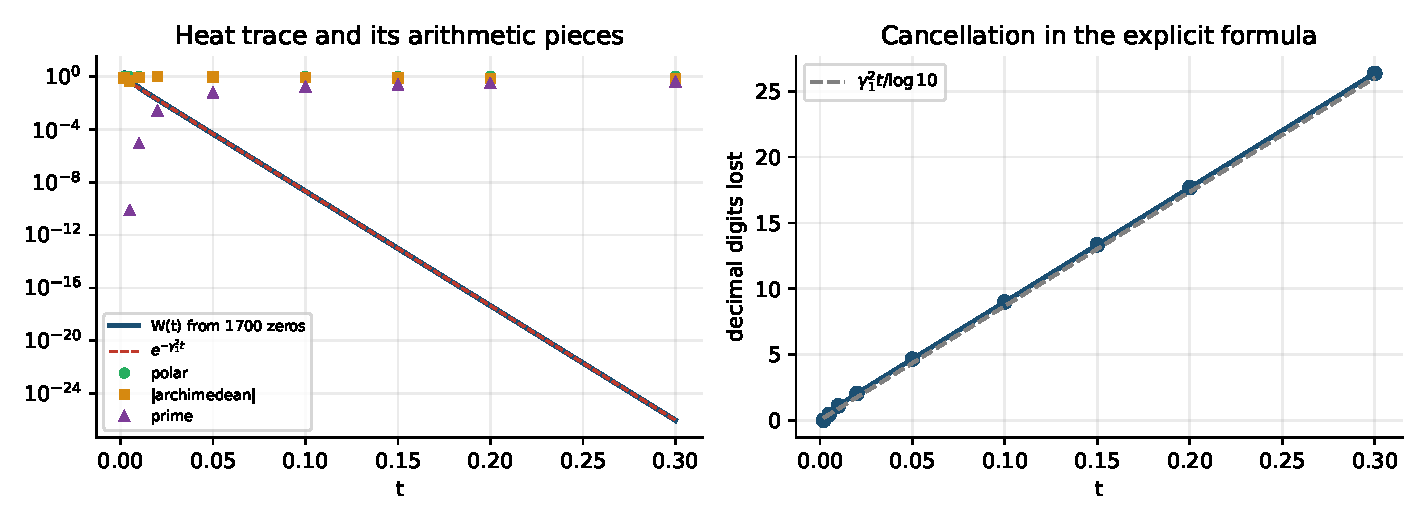
\includegraphics[width=\textwidth]{fig/heattrace.pdf}
\caption{Left: the heat trace from $1700$ zeros, its leading exponential $e^{-\gamma_1^2t}$, and the three arithmetic pieces, the archimedean one in absolute value. Right: digits lost to cancellation in the explicit formula; for $t\ge0.05$ they lie $\log_{10}2+t/(4\log10)$ above the dashed line $\gamma_1^2t/\log10$.}
\label{fig:ch14:W}
\end{figure}

The explicit formula holds exactly, and the cancellation costs working precision and nothing more: $26.4$ digits at $t=0.3$, well within sixty digit arithmetic. It is the price of computing an exponentially small quantity as a difference of terms of size $e^{t/4}$, the price the untilted P\'olya route pays at height $\theta$, where it loses $0.341\,\theta$ digits (Section~\ref{ch:polya}). The zeros give $W$ cheaply at moderate $t$, the primes only near $t=0$. Section~\ref{ch:sato} finds the same profile for the L\'evy density $-W'$ of the subordinator that drives the clock.

The two descriptions divide the work. The arithmetic side is cheap where $g$ is concentrated near $x=0$, so that only small $n$ contribute: at small $t$ for the heat kernel, and only at large resolution for the Poisson kernel $h(r)=P_\varepsilon(\theta-r)+P_\varepsilon(\theta+r)$. That kernel is not in $\mathcal T$, but for $\varepsilon>\frac12$ its transform $g(x)=\pi^{-1}e^{-\varepsilon|x|}\cos\theta x$ makes the prime sum converge absolutely; for smaller $\varepsilon$ the prime side is Selberg's smoothed sum, which with cutoff $X$ uses the primes up to $X^2$ and has error of order $X^{-\varepsilon}/(\varepsilon^2\log X)$ when no zero lies to the right of the critical line, the single zero law of Section~\ref{sec:ch10:selberg}. The spectral side is cheap where the test function is concentrated at the low zeros: at large $t$, and at small $\varepsilon$ on a window. In the proofs of the lower rungs in Section~\ref{ch:heat} the two forms meet at $t=1/20000$, where the inequalities are checked in interval arithmetic. The Thorin condition requires positivity at every scale, and neither side is cheap at every scale. The P\'olya route of Section~\ref{ch:polya} is, but only on a window of finite height, and that restriction is the barrier of Section~\ref{ch:finite}.

\section{Spacings, irregularity and the cell distance}\label{ch:spacing}

On a window of finite height the errors of the P\'olya route, measured by the cell distance $d_{\rm cell}(\varepsilon)$ of Section~\ref{ch:distances}, are set by the spacings of the zeros, which follow the random matrix prediction already for the first $1700$ zeros.

\subsection{The cell distance to first order}\label{sec:ch15:first}

We use the cells $C_k=(b_{k-1},b_k]$ of Section~\ref{sec:ch7:cumulative}, with $\Theta=200$ and $K=N(\Theta)=79$, and the first order formula for $\mu_\varepsilon(C_k)-1$ derived there, whose remainder is $O(\varepsilon^3)$ (Remark~\ref{rem:ch7:cubic}); Exercise~\ref{ex:ch15:odd} gives its leading term. The formula needs only that the zeros below $\Theta$ be simple and on the line.

Under RH the formula becomes a sum over the ordinates. By Proposition~\ref{prop:struct}, $\rho_\varepsilon(\theta)=\sum_j[P_\varepsilon(\theta-\gamma_j)+P_\varepsilon(\theta+\gamma_j)]$ over all positive ordinates, and the kernel $P_\varepsilon(\cdot-\gamma)$ has distribution function $F_\varepsilon(y-\gamma)$, where $F_\varepsilon(y)=\frac12+\frac1\pi\arctan(y/\varepsilon)=\mathbf 1_{y\ge0}-\varepsilon/(\pi y)+O(\varepsilon^3/|y|^3)$ as $\varepsilon/|y|\to0$. No ordinate lies on a cell boundary, so
\[
\mu_\varepsilon(C_k)-1=-\frac\varepsilon\pi\sum_j\Big[\frac1{b_k-\gamma_j}-\frac1{b_{k-1}-\gamma_j}+\frac1{b_k+\gamma_j}-\frac1{b_{k-1}+\gamma_j}\Big]+O(\varepsilon^3),
\]
and by \eqref{eq:ch2:hadamard} with $s=i\theta$, $\Xi'/\Xi(\theta)=\sum_j[(\theta-\gamma_j)^{-1}+(\theta+\gamma_j)^{-1}]$ under RH, so the two expansions agree. Summing absolute values,
\[
\begin{aligned}
d_{\rm cell}(\varepsilon)&=\kappa_{\rm cell}\,\varepsilon+O(\varepsilon^3),\\
\kappa_{\rm cell}&=\frac1\pi\sum_k\Big|\sum_j\Big[\frac1{b_k-\gamma_j}-\frac1{b_{k-1}-\gamma_j}+\frac1{b_k+\gamma_j}-\frac1{b_{k-1}+\gamma_j}\Big]\Big| .
\end{aligned}
\]

Truncated to the first $1700$ ordinates, the zero sum gives $5.415$, against $\kappa_{\rm cell}=5.43665$ from the form in $\Xi'/\Xi$ and the observed slope $d_{\rm cell}(0.005)/0.005=5.43664$. The difference of $0.4$ per cent between $5.415$ and $5.43665$ is the contribution of the zeros above $\gamma_{1700}$. In the truncated formula the cell errors range from $-0.225\,\varepsilon$ to $+0.250\,\varepsilon$ (Figure~\ref{fig:ch15:cells}), with the two largest positive values at the end cells: at the last because $\Theta$ is not a midpoint between ordinates, and at the first because below $b_1$ there is only $\gamma_1$ and then the reflections $-\gamma_j$, which do not balance the zeros above $b_1$.

\begin{figure}[htbp]
\centering
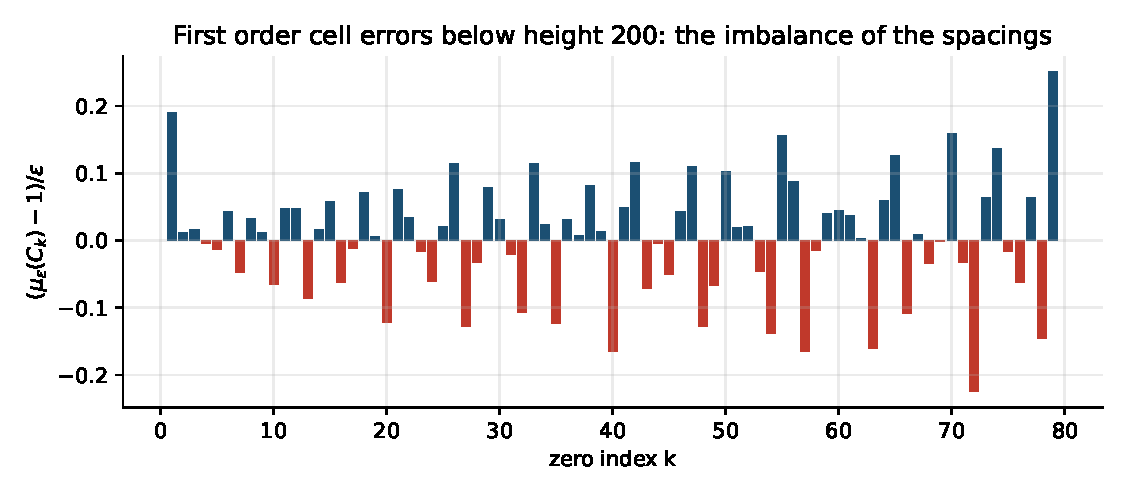
\includegraphics[width=0.85\textwidth]{fig/cells.pdf}
\caption{First order cell errors $(\mu_\varepsilon(C_k)-1)/\varepsilon$ for the $79$ cells below height $200$, computed from the first $1700$ ordinates.}
\label{fig:ch15:cells}
\end{figure}

The atoms $\theta=k\ge1$ of the sinh benchmark of Section~\ref{ch:ggc} and their reflections form the lattice $\mathbb Z$ without the point $0$. For the full lattice every cell $(k-\frac12,k+\frac12]$ would have mass exactly one, by periodicity, so the deficit of each cell is the mass that the missing kernel at $0$ would have put in it; the atom free interval $(0,\frac12]$, which the benchmark counts as a cell of mass zero, receives the mass $\frac12$ of the full lattice less that of the missing kernel:
\[
\mu_\varepsilon\big((k-\tfrac12,k+\tfrac12]\big)=1-\frac1\pi\arctan\frac{\varepsilon}{\varepsilon^2+k^2-\frac14},\qquad \mu_\varepsilon\big((0,\tfrac12]\big)=\frac1\pi\arctan(2\varepsilon).
\]
The interior cells therefore do not balance: each loses $\varepsilon/(\pi(k^2-\frac14))+O(\varepsilon^3)$, while $(0,\frac12]$ gains $2\varepsilon/\pi+O(\varepsilon^3)$. As $\sum_{k\le N}(k^2-\frac14)^{-1}=2-1/(N+\frac12)$, the cell distance of $N$ atoms is $(4-1/(N+\frac12))\,\varepsilon/\pi+O(\varepsilon^3)$, which is $1.26694\,\varepsilon$ for $N=50$, the constant $1.267$ of Section~\ref{ch:ggc}. With the convention used for the zeros, a first cell $(0,\frac32]$, it would be $(\frac43-1/(N+\frac12))/\pi=0.418$. For the zeros no cell is balanced, and the errors in Figure~\ref{fig:ch15:cells} do not decay along the window.

The constant vanishes exactly when the sum of $1/(b-x)$ over the ordinates and their reflections vanishes at every cell boundary $b$, as it does when these points are symmetric about every boundary. The lattice $\gamma_j=(j-\frac12)h$, whose reflections complete $(\mathbb Z+\frac12)h$, has every cell error zero, whereas the lattice of the benchmark does not. For the zeros every ordinate contributes to a cell error, with a weight that decays like $|C_k|/(\gamma_j-b_k)^2$. The two ordinates nearest an interior boundary are symmetric about it, so the asymmetry comes first from the next gaps on either side, and it is small when those gaps are equal.

\subsection{Spacings of the zeros and the Thorin density}\label{sec:ch15:spacings}

At height $\gamma$ the mean spacing of the zeros is $\Delta=2\pi/\log(\gamma/2\pi)$, as in Section~\ref{sec:ch13:visibility}. We unfold by $\tilde\gamma=\vartheta(\gamma)/\pi$. The $1699$ normalised spacings $\tilde\gamma_{k+1}-\tilde\gamma_k$ of the first $1700$ zeros, which lie below height $2198$, have variance $0.146$ and minimum $0.089$. Figure~\ref{fig:ch15:spacing} compares their histogram with the Wigner surmise for the Gaussian unitary ensemble, $p_{\rm W}(s)=\frac{32}{\pi^2}s^2e^{-4s^2/\pi}$, and with the Poisson law $e^{-s}$ of independent points. The histogram follows the surmise already at this height, including the quadratic repulsion at small spacings that Montgomery's pair correlation conjecture predicts \cite[pp.~183 and 184]{Montgomery73} and that Odlyzko observed at large height \cite{Odlyzko87}. The variance is below the surmise value $3\pi/8-1=0.178$; the spacing distribution approaches the unitary one only slowly with height \cite[p.~185]{Montgomery73}, \cite[Section 3]{BBLM06}.

\begin{figure}[htbp]
\centering
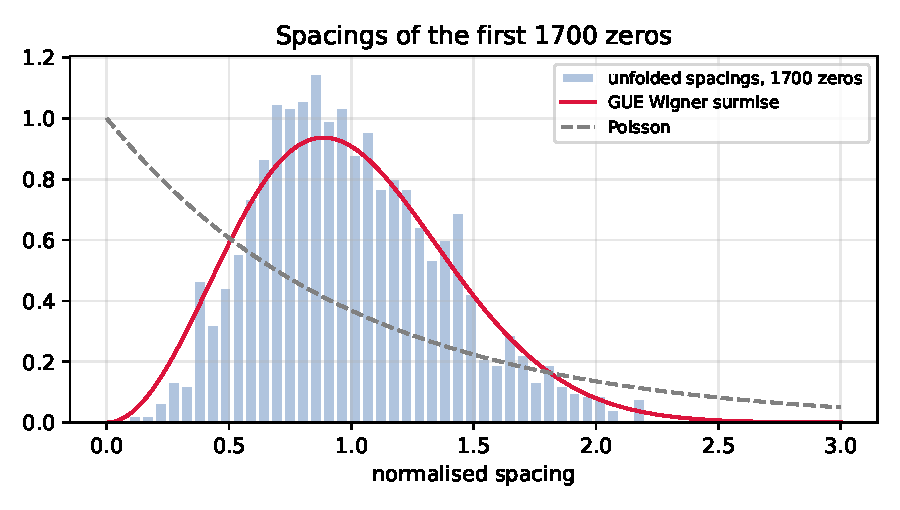
\includegraphics[width=0.72\textwidth]{fig/spacing.pdf}
\caption{The $1699$ unfolded spacings of the first $1700$ zeros against the GUE Wigner surmise and the Poisson law.}
\label{fig:ch15:spacing}
\end{figure}

Repulsion affects the Thorin density in two ways. First, it makes very small gaps rare but not absent. The smallest normalised spacing among the first $1700$ zeros, $0.089$, separates the ordinates $1977.17$ and $1977.27$, the pair that Section~\ref{ch:finite} moves off the line in Figure~\ref{fig:ch13:perturb}. By the Cauchy kernel criterion of Exercise~\ref{ex:ch5:cauchy}, an isolated pair of ordinates at distance $g$ in $\theta$ gives two peaks of $\rho_\varepsilon$ only for $\varepsilon<\sqrt3g/2$. The resolution needed to separate every pair on a window is therefore set by the smallest gap, and repulsion controls it: if the $N$ normalised spacings were independent, with density $p_{\rm W}(s)\propto s^2$ near zero, the smallest would be of order $N^{-1/3}$, which is $0.084$ for $N=1699$, close to the observed $0.089$.

Second, repulsion sets the scale of the local visibility condition of Section~\ref{sec:ch13:visibility}: to first order in $\varepsilon$, an off line zero at distance $d$ from the line makes $\rho_\varepsilon$ negative at its ordinate if and only if $2/d^2$ exceeds $\sum_j\delta_j^{-2}$, where $\delta_j$ are the distances from its ordinate to the other ordinates. The sum is dominated by the nearest neighbours, and repulsion makes it typically of order $\Delta^{-2}$, because $\E s^{-2}$ is finite for the surmise, where it equals $8/\pi$, and infinite for the Poisson law. With neighbours on a lattice of spacing $\Delta$, the density at the ordinate stays positive at small resolution once $d$ exceeds the threshold $(\sqrt6/\pi)\Delta\approx0.78\,\Delta$ of that section. Since $d<\frac12$, a zero hidden in this way can exist only where $\Delta<0.64$, that is above height about $1.1\times10^5$. Hidden here means hidden at the ordinate: beside it the density can be negative even when the condition predicts a positive value there (Exercise~\ref{ex:ch15:beside}).

The behaviour of the cell constant at large height is open (Section~\ref{ch:open}). In unfolded units the cell errors depend mainly on the nearby ordinates, so the sine kernel process of the unitary ensemble would predict their mean and fluctuations per cell; we have not computed that prediction. Computing the cell errors with Odlyzko's zeros near zero number $10^{12}$ \cite{Odlyzko87}, $10^{21}$ or $10^{22}$ \cite{Odlyzko01,OdlyzkoTables}, at heights about $2.7\times10^{11}$, $1.4\times10^{20}$ and $1.4\times10^{21}$, would compare the Thorin density with the spacing statistics of the zeros at large height. It needs the ordinates, which define the cells, and the hybrid evaluator of Section~\ref{sec:ch5:hybrid} for $\Xi'/\Xi$ at the cell boundaries. Section~\ref{ag:sec:margins} proposes the same comparison at large height for the positivity margins of the density, its values at the midpoints between consecutive ordinates.

\section{Exercises}\label{chap:heat:ex}

\paragraph{On Section~\ref{ch:heat}.}
\begin{exercises}
\item Show that $c_0c_2-c_1^2=\frac12\sum_{j,l}(a_j-a_l)^2e^{-(a_j+a_l)t}$ and deduce that log convexity of $W$ holds under RH.
\item Recompute the first row of Table~\ref{tab:ch12:hankel} with the first $100$ zeros and explain why no printed digit changes.
\item Show that for a real exponent $a$ the summand of the Williamson measure $U_k$ belonging to $a$ is the inverse gamma density of $ka/\Gamma_k$ with $\Gamma_k\sim$ Gamma$(k,1)$, and compute its variance for $k>2$.
\item\label{ex:ch12:toy} Let $\widetilde W(t)=e^{-t}+2e^{-10t}\cos t$, the heat trace of the three exponents $1$ and $10\pm i$. Show that $\widetilde W>0$ and $\widetilde W'<0$ on $(0,\infty)$, using $\cos t>0$ and $\sin t\ge0$ for $t\le1$ and $2\sqrt{101}\,e^{-9}<1$ for $t\ge1$, so that the first two rungs of Theorem~\ref{thm:ch12:idsd} hold. With $\theta=\arctan\frac1{10}$, show that $\frac{10}{101}<\theta<\frac1{10}$, hence $\frac{2\pi}3<24\theta<\pi$, and deduce that $(-1)^{24}\widetilde W^{(24)}(0)=1+2\cdot101^{12}\cos24\theta<0$, so that $\widetilde W$ is not completely monotone. Then check numerically that the first order $k$ at which $(-1)^k\widetilde W^{(k)}(t)<0$ for some $t>0$ is $12$, near $t=2.87$, and compare with the first failures of Table~\ref{tab:ch13:first}.
\item Show that the term of order $1/u$ of $\varepsilon_\rho$ in Proposition~\ref{prop:ch12:ray} is $\frac{2t}{3u}(\tilde\gamma-u)^3$. For $u=2$, $t=1$ and $k=4$, show that no zero lies in the disc $|\tilde\gamma-u|\le u/2$, so that $c_4(1)=e^{f_0}R$ is carried entirely by the remainder, and compare the bound on $R$ with the contribution of the first zero.
\item Show that $m(0)>-6$ and, comparing the series for $\psi$ with an integral, that $m(60)>1$. Deduce that for $t\le10^{-6}$ the archimedean term of \eqref{eq:ch2:Warith} is at least $1/(4\sqrt{\pi t})-210/\pi>55$ and the prime term at most $(\pi t)^{-1/2}e^{-(\log2)^2/4t}<0.01$. With the argument of the proof of Theorem~\ref{thm:ch12:idsd} for $t\ge\tau$, taken at height $10^4$ and from $t=10^{-6}$, conclude that $W>0$ on $(0,\infty)$ follows from the verification of RH below height $10^4$ by estimates that can all be checked by hand.
\end{exercises}

\paragraph{On Section~\ref{ch:arith}.}
\begin{exercises}
\item Verify the arithmetic form of $W(t)$ at $t=0.01$ with the prime powers up to $10^4$, and explain why so few suffice by showing that only $n=2$ and $n=3$ affect the first fifteen digits.
\item\label{ex:ch14:law} Show that $m$ increases on $[0,\infty)$ and vanishes at a single point $r_*$, and deduce that $e^{r_*^2t}A(t)$ decreases in $t$, so that $A$ changes sign at most once; with Table~\ref{tab:ch14:W}, conclude that $A<0$ for $t\ge0.005$. Then show that for $t\ge0.05$ the number of digits lost in the table equals $\log_{10}2+(\gamma_1^2+\frac14)t/\log10$ up to an exponentially small error, and identify the source of each term.
\item Show that the regularised constants of the gamma, pole and prime parts of the variogram form sum to zero if and only if $\xi'(\frac12)=0$.
\end{exercises}

\paragraph{On Section~\ref{ch:spacing}.}
\begin{exercises}
\item\label{ex:ch15:odd} Let $\ell=\Xi'/\Xi$. Show that $\xi(\frac12+\varepsilon+ib)=\Xi(b-i\varepsilon)$, and deduce from the Taylor series of $\log\Xi$ about $b$ that $\mu_\varepsilon(C_k)-1=-\frac\varepsilon\pi[\ell(b_k)-\ell(b_{k-1})]+\frac{\varepsilon^3}{6\pi}[\ell''(b_k)-\ell''(b_{k-1})]+O(\varepsilon^5)$. Under RH, check that the term in $\varepsilon^3$ agrees with the expansion of $F_\varepsilon$ to third order.
\item Prove the arctangent formulas for the cell masses of the sinh benchmark, and deduce that its cell distance for $N$ atoms is $(4-1/(N+\frac12))\,\varepsilon/\pi+O(\varepsilon^3)$, and $(\frac43-1/(N+\frac12))\,\varepsilon/\pi+O(\varepsilon^3)$ when the first cell is $(0,\frac32]$.
\item Show that the Wigner surmise $p_{\rm W}$ has mean $1$ and variance $3\pi/8-1$, and that $\E s^{-2}=8/\pi$ under it, while $\E s^{-2}=\infty$ for the Poisson law.
\item Show that $\sum_{m\ne0}(m\Delta)^{-2}=\pi^2/(3\Delta^2)$, deduce the lattice threshold $(\sqrt6/\pi)\Delta$ of the visibility condition, and find the height above which the threshold is less than $\frac12$.
\item\label{ex:ch15:beside} In a local model, put an off line pair at distance $d=0.3$ from the line at the ordinate $\gamma$ and zeros on the line at $\gamma+0.2+m$ and $\gamma-4-m$ for $m\ge0$, and ignore the reflected kernels. At $\varepsilon=0.005$, show that $2/d^2<\sum_j\delta_j^{-2}$, so that the visibility condition predicts a positive density at $\gamma$, and check that $\rho_\varepsilon(\gamma)>0$ while $\rho_\varepsilon(\gamma-0.079)<0$.
\end{exercises}

\chapter{The reciprocal zeta function}\label{chap:rzeta}

The reciprocal zeta function $1/\zeta(\frac12+\sqrt s)$ is, up to the factor $1-4s$ of the pole and a constant, the reciprocal Xi function times the gamma factor, and unlike $\xi$ it has a Dirichlet series and an Euler product, from which we read its Thorin type measures.

Sections~\ref{ch:rz1} and \ref{ch:rz2} compute the Thorin measure of the gamma factor, the Thorin measures of the normalised reciprocal zeta function and of the reciprocal Xi function under RH, and, unconditionally, the formal Thorin measures of these two functions in the Vere-Jones form of Section~\ref{rz:sec:lvj}. After the stable tilt $e^{-c\sqrt s}$, with $c=\zeta'(\frac12)/\zeta(\frac12)$, the reciprocal of the gamma factor is a generalised gamma convolution, and multiplying the normalised reciprocal zeta function by it gives the floor $e^{-c\sqrt s}\,\xi(\frac12)/\xi(\frac12+\sqrt s)$ of the reciprocal Xi function (Section~\ref{rz:sec:floor}), in which the zeros are the only possible source of negativity.

The infinite divisibility of the floor, as proved here, rests on the positivity of the canonical function of the normalised reciprocal zeta function, which is Theorem~\ref{rz:thm:id} of Chapter~\ref{chap:rzid}. It also follows from the infinite divisibility of the clock (Theorem~\ref{thm:ch12:idsd}); what the floor adds is a splitting of its canonical function into an arithmetic part and a completely monotone archimedean part. The floor is a generalised gamma convolution exactly when RH holds, and the derivatives of its canonical function alternate in sign up to order $10^{10}$ by the methods of this chapter and up to order $1.16\times10^{25}$ by the estimates of Section~\ref{ch:heat}.

\section{Thorin type forms of the reciprocal zeta function}\label{ch:rz1}

Stieltjes inversion gives the Thorin type measure of a single Euler factor, a cosine series of both signs. The Lai and Vere-Jones identity replaces the exponentials of the Dirichlet series by hyperbolic secants, whose Thorin measures are lattices of unit atoms, at the price of M\"obius signs in the coefficients. Under RH the Thorin measure of the normalised reciprocal zeta function is $dM$, where $M-1$ is the argument function $S(\sqrt t)$. Its heat trace, the canonical function $w$ of Theorem~\ref{rz:thm:w}, is explicit in the primes, is an absolutely convergent series of Jacobi theta functions, and gives a criterion for RH (Theorem~\ref{rz:thm:crit}). Section~\ref{rz:sec:strip} follows these objects across the critical strip.

\subsection{The question and the three functions}\label{rz:sec:intro}

Write $\sqs$ for the principal square root on the cut plane $\cut$, so that $\Re\sqs>0$ there, and evaluate $\zeta$ at $z=\frac12+\sqs$. A zero $\rho=\frac12+i\gamma$ then corresponds to $\sqs=i\gamma$, that is to $s=-\gamma^2$, a point of the cut, and an atom of a Thorin measure at $t$ produces a singularity at $s=-t$, also on the cut. The Riemann Hypothesis therefore says that every zero sits where a Thorin atom could sit, which is the reason for the variable $\sqs$ here, as in Section~\ref{ch:clock}. The question of this chapter and of Chapter~\ref{chap:rzid} is whether the zeros, the primes and the gamma factor assemble into a Thorin measure, and if so which one. The two chapters have their own coordinates, which hold throughout both unless stated otherwise: $s$ is the variable $u$ of Sections~\ref{ch:clock} and \ref{ch:ggc}, $t$ is the variable $z$ of their Thorin measures, $x$ is the time of the heat trace $W(x)$, $\tau$ is the ordinate, and $z$ is the argument of $\zeta$ and $\xi$.

The M\"obius series and the Euler product converge absolutely to the right of the parabola $x=\frac14-y^2$, on
\[
H_{1/2}=\{s:\Re\sqs>\tfrac12\}=\{x+iy:\ x>\tfrac14-y^2\},
\]
and there
\begin{equation}\label{rz:eq:basic}
\frac{1}{\zeta(\frac12+\sqs)}=\sum_{n\ge1}\frac{\mu(n)}{\sqrt n}\,e^{-\sqs\log n}
=\prod_{p}\Bigl(1-p^{-1/2}e^{-\sqs\log p}\Bigr).
\end{equation}
Every term is built from $e^{-\lambda\sqs}$, which is completely monotone in $s$: it is the Laplace transform of the positive stable law of index $\frac12$, the law of the first passage time of $\sqrt2B$ to the level $\lambda$, where $B$ is a standard Brownian motion,
\begin{equation}\label{rz:eq:levy}
e^{-\lambda\sqs}=\int_0^\infty e^{-sx}\,\frac{\lambda}{2\sqrt\pi}\,x^{-3/2}e^{-\lambda^2/4x}\,dx .
\end{equation}
So \eqref{rz:eq:basic} writes $1/\zeta(\frac12+\sqs)$ as a signed series of Laplace transforms of stable laws. The Thorin measure, however, is read from the logarithm. Recall from \eqref{eq:ch3:ggc} that a generalised gamma convolution (GGC) has Laplace transform
\begin{equation}\label{rz:eq:thorin}
f(s)=\exp\Bigl(-as-\int_{(0,\infty)}\log\bigl(1+\tfrac st\bigr)\,U(dt)\Bigr),
\end{equation}
with $a\ge0$ and $U\ge0$ the Thorin measure; equivalently $-f'/f(s)=a+\int U(dt)/(s+t)$ is a Stieltjes function \cite{Bondesson}. We allow $U$ to be signed, with $\int_{(0,1)}|\log t|\,|U|(dt)+\int_{[1,\infty)}t^{-1}|U|(dt)<\infty$ so that the integral converges, and then call \eqref{rz:eq:thorin} a Thorin type representation.

Three functions of $s$ run through both chapters. The function $1/\zeta(\frac12+\sqs)$ vanishes at $s=\frac14$, where $\zeta$ has its pole, and equals $1/\zeta(\frac12)<0$ at $s=0$, so it is not the Laplace transform of a probability law. Both defects are removed by the normalised reciprocal zeta function
\begin{equation}\label{rz:eq:phi}
\varphi(s)=\frac{\zeta(\frac12)}{(1-4s)\,\zeta(\frac12+\sqs)},\qquad \varphi(0)=1 .
\end{equation}
The other two are the gamma factor $G(s)=\Gamma(\frac14+\frac\sqs2)\pi^{-\sqs/2}/\Gamma(\frac14)$ and the reciprocal Xi function $R(s)=\xi(\frac12)/\xi(\frac12+\sqs)$, and $\varphi=RG$ (Proposition~\ref{rz:prop:rh}). In both chapters $G$ is the gamma factor, not the function $G$ of Section~\ref{ch:clock}, whose reciprocal is $R$, except in Section~\ref{rz:sec:polya}, where $G$ is a Laguerre P\'olya function; and $\theta(\tau)=\Im\log\Gamma(\frac14+\frac{i\tau}{2})-\frac\tau2\log\pi$ is the Riemann Siegel theta function, written $\vartheta$ elsewhere in the book (Section~\ref{ch:classical}), so that $\theta'(\tau)=\frac12\Re\psi(\frac14+\frac{i\tau}2)-\frac12\log\pi$ \cite[Section 6.5]{Edwards}. Table~\ref{rz:tab:measures} lists the Thorin measures of the three functions and of the building blocks used below. In it $N(T)$ counts the zeros with $0<\gamma\le T$, $S(T)=\pi^{-1}\arg\zeta(\frac12+iT)$ is the argument function, $c_n=2n+\frac12$, $c=-\theta'(0)$ is the constant of \eqref{rz:eq:c}, and $U_\lambda$ is the sawtooth measure of Lemma~\ref{rz:lem:saw}.

\begin{table}[htbp]
\centering
\small
\begin{tabular}{lll}
\toprule
Function & Thorin measure & Sign\\
\midrule
$\varphi$ & $dM(t)$, $M(t)=N(\sqrt t)-\theta(\sqrt t)/\pi=1+S(\sqrt t)$ (RH) & signed\\
$G$ & $-\dfrac{\theta'(\sqrt t)}{2\pi\sqrt t}dt=\dfrac{1}{2\pi\sqrt t}\Bigl\{b+\sum_{n\ge0}\Bigl(\dfrac{c_n}{t+c_n^2}-\dfrac1{2n+2}\Bigr)\Bigr\}dt$ & signed\\
$R$ & $\sum_{\gamma>0}\delta_{\gamma^2}$ (RH) & positive\\
\midrule
$2/(1+e^{-\lambda\sqs})$ & $-U_\lambda=\sum_k\delta_{((2k+1)\pi/\lambda)^2}-\dfrac{\lambda}{4\pi\sqrt t}dt$ & signed\\
$(1+\sqs/\kappa)^{-1}$ & $\dfrac{\kappa}{2\pi\sqrt t\,(t+\kappa^2)}dt$ & positive\\
$\sech(\lambda\sqs)$ & $\sum_k\delta_{((k+\frac12)\pi/\lambda)^2}$ & positive\\
$e^{-c\sqs}/G$ & $\dfrac{\theta'(\sqrt t)-\theta'(0)}{2\pi\sqrt t}dt$ & positive\\
\bottomrule
\end{tabular}
\caption{Thorin measures of $\varphi$, $G$ and $R$ and of the building blocks used in this chapter and in Chapter~\ref{chap:rzid}, with the convention $\log f(s)=-\int\log(1+s/t)\,U(dt)$ after normalising $f(0)=1$. Here $b=\frac12(\gamma_E+\log\pi)$, $\kappa>0$ and $c=-\theta'(0)=\zeta'(\frac12)/\zeta(\frac12)$. The rows for $\varphi$ and $R$ are Theorem~\ref{rz:thm:thorin}, the row for $G$ is Theorem~\ref{rz:thm:gamma}, the fourth row is Lemma~\ref{rz:lem:saw}, the fifth and sixth appear in Table~\ref{tab:ch3:cat}, and the last is Theorem~\ref{rz:thm:gammaggc}.}
\label{rz:tab:measures}
\end{table}

\subsection{Stieltjes inversion and the Euler factors}\label{rz:sec:prelim}

Three descriptions of a function $F$ on the cut plane recur: its Thorin measure $U$, the Stieltjes representation $-F'/F(s)=\int U(dt)/(s+t)$, and the boundary values of $-F'/F$ on $(-\infty,0]$. Lemma~\ref{rz:lem:inv} recovers the measure from the boundary values. It computes most of the Thorin measures of this chapter and of Chapter~\ref{chap:rzid}, and in each application the work is to evaluate $\Im f(-t+i0)$ for $f=-F'/F$, which amounts to putting $\sqs=i\sqrt t$.

\begin{lemma}\label{rz:lem:inv}
Let $f$ be analytic on $\cut$ with $f(\bar s)=\overline{f(s)}$, $f(s)\to0$ as $|s|\to\infty$ uniformly in $\arg s$, $|f(s)|\le C|s|^{-\alpha}$ near $0$ for some $\alpha<1$, and such that $f$ extends continuously from the upper half plane to the points of $(-\infty,0)$ apart from finitely many points $-t_0$, at each of which $f(s)-r/(s+t_0)$ is bounded near $-t_0$ in $\cut$ for some real $r$; $f(-t+i0)$ denotes the values of this extension and $f(-t-i0)=\overline{f(-t+i0)}$. Then
\[
f(s)=\int_{(0,\infty)}\frac{m(dt)}{s+t},\qquad m(dt)=-\frac1\pi\,\Im f(-t+i0)\,dt,
\]
where the integral is the limit of the integrals over $(0,T]$ as $T\to\infty$, absolutely convergent when $\int_{(1,\infty)}t^{-1}|m|(dt)<\infty$, and where each of the points $-t_0$, which we call a simple pole of $f$, contributes the atom $r\,\delta_{t_0}$ to $m$.
\end{lemma}

\begin{proof}
Fix $s\in\cut$ and integrate $f(z)/(z-s)$ over a keyhole contour around $(-\infty,0]$, which by Cauchy's formula gives $2\pi i\,f(s)$; the large circle vanishes by the decay at infinity and the small circle by the bound at the origin. By the continuity of the extension, the integrals along the two sides of the keyhole converge to the integrals of the boundary values as the keyhole closes onto the cut, after subtracting $r/(z+t_0)$ near each pole $-t_0$, where the remainder is bounded. The two sides of the cut combine to $\frac{1}{2\pi i}\{f(-t-i0)-f(-t+i0)\}=-\frac1\pi\Im f(-t+i0)$. At a simple pole the contour follows small semicircles above and below the cut, which together contribute $r/(s+t_0)$.
\end{proof}

The hypotheses of uniform decay at infinity and of finitely many poles exclude functions with infinitely many poles on the cut, such as $-R'/R$ under RH, which has a pole at every $-\gamma^2$, and $-R_\sigma'/R_\sigma$ for the functions $R_\sigma$ of Section~\ref{rz:sec:strip} when no zero lies to the right of the line $\Re z=\sigma$ and infinitely many lie on it. Such an application needs a direct argument from Hadamard's product, as in the proof of Theorem~\ref{rz:thm:thorin}.

For $f(s)=\lambda e^{-\lambda\sqs}/(2\sqs)=-\frac{d}{ds}e^{-\lambda\sqs}$ one has $\sqrt{-t+i0}=i\sqrt t$, and the lemma gives the density $\frac{\lambda}{2\pi\sqrt t}\cos(\lambda\sqrt t)$, so that
\[
e^{-\lambda\sqs}=1-\int_0^\infty\log\bigl(1+\tfrac st\bigr)\frac{\lambda\cos(\lambda\sqrt t)}{2\pi\sqrt t}\,dt .
\]
This is not the Thorin measure of $e^{-\lambda\sqs}$, which is the positive density $\lambda/(2\pi\sqrt t)$ (Table~\ref{tab:ch3:cat}), but the Thorin type density that an exponential contributes when it sits in an exponent, as it does in the logarithm of every Euler factor of \eqref{rz:eq:basic} and in $\log\zeta(\frac12+\sqs)$. It oscillates in sign, and this is the difficulty: every Euler factor has a signed Thorin density, and any positivity must come from the product. The Euler factors show this in closed form.

\begin{proposition}\label{rz:prop:euler}
For $0<q<1$ and $\lambda>0$ the Euler factor $E(s)=1-qe^{-\lambda\sqs}$ is analytic and zero free on $\cut$, and
\[
\log\frac{E(s)}{1-q}=-\int_0^\infty\log\bigl(1+\tfrac st\bigr)\,u(t)\,dt,
\]
\[
u(t)=-\frac{q\lambda}{2\pi\sqrt t}\,\frac{\cos(\lambda\sqrt t)-q}{1-2q\cos(\lambda\sqrt t)+q^2}
=-\frac{\lambda}{2\pi\sqrt t}\sum_{k\ge1}q^k\cos(k\lambda\sqrt t).
\]
\end{proposition}

\begin{proof}
On $\cut$ we have $|e^{\lambda\sqs}|>1>q$, so $E$ has no zeros. Put $f=-E'/E=-\frac{q\lambda}{2\sqs}(e^{\lambda\sqs}-q)^{-1}$, which is $O(|s|^{-1/2})$ at $0$ and decays at infinity. At $\sqs=i\tau$, $\tau=\sqrt t$, we get $f=\frac{iq\lambda}{2\tau}(e^{i\lambda\tau}-q)^{-1}$ and $\Im f=\frac{q\lambda}{2\tau}\,\frac{\cos\lambda\tau-q}{1-2q\cos\lambda\tau+q^2}$. Lemma~\ref{rz:lem:inv} gives $u$; integrating $-E'/E=\int u(t)\,dt/(s+t)$ from $0$ to $s$ gives the logarithm, and the series is the Poisson kernel expansion.
\end{proof}

With $q=p^{-1/2}$ and $\lambda=\log p$, summing $u$ over $p$ formally gives
\begin{equation}\label{rz:eq:formal}
u_\zeta(t)=-\frac{1}{2\pi\sqrt t}\sum_{n\ge2}\frac{\Lambda(n)}{\sqrt n}\cos(\sqrt t\log n)
\;\;\text{``}=\text{''}\;\;\frac{1}{2\pi\sqrt t}\,\Re\frac{\zeta'}{\zeta}\bigl(\tfrac12+i\sqrt t\bigr),
\end{equation}
a divergent series. Since $\frac{d}{d\tau}\arg\zeta(\frac12+i\tau)=\Re\frac{\zeta'}{\zeta}(\frac12+i\tau)$, the right side is formally the density of $dS(\sqrt t)$, but the series converges only in the sense of distributions. Theorem~\ref{rz:thm:thorin} makes this precise, and Theorem~\ref{rz:thm:w} replaces the divergent cosine series by a convergent Gaussian one.

\subsection{The Lai and Vere-Jones identity and sawtooth measures}\label{rz:sec:lvj}

Each exponential in $\log\zeta$ contributes an oscillating Thorin type density (Section~\ref{rz:sec:prelim}). We trade each exponential for a hyperbolic secant, whose Thorin measure is a lattice of unit atoms, at the price of a M\"obius inversion. This is done twice: additively in the Dirichlet series of $1/\zeta$ (Theorem~\ref{rz:thm:sech}), and logarithmically in $\log\zeta$, where Thorin measures are defined, with $\log(1+e^{-x})$ in place of the secant (Theorem~\ref{rz:thm:saw}).

Lai and Vere-Jones \cite{LVJ} pose the completeness of the dilates $\sech(\theta x)$, $\theta\ge0$, as an open problem for the hyperbolic secant law. The M\"obius inversion of the alternating exponential series of the secant expands $e^{-x}$ in the dilates $\sech(mx)$. This is Proposition~\ref{rz:prop:lvj}, which we call the Lai and Vere-Jones identity, and the expansions of $1/\zeta$ and $\log\zeta$ built from it form the Vere-Jones representation. Here $\chi_4$ is the nontrivial character modulo $4$.

\begin{proposition}\label{rz:prop:lvj}
For $\Re x>0$,
\[
\tfrac12\sech x=\sum_{m\ \mathrm{odd}}\chi_4(m)\,e^{-mx},
\qquad
e^{-x}=\tfrac12\sum_{m\ge1}\mu(m)\chi_4(m)\,\sech(mx).
\]
\end{proposition}

\begin{proof}
The first is the geometric series $e^{-x}/(1+e^{-2x})$. Since $\chi_4$ is completely multiplicative, $\sum_m\mu(m)\chi_4(m)\sum_k\chi_4(k)e^{-mkx}=\sum_r e^{-rx}\sum_{mk=r}\mu(m)\chi_4(m)\chi_4(k)=e^{-x}$, the rearrangement being justified by $\sum_{m,k}e^{-mk\Re x}<\infty$ for $\Re x>0$.
\end{proof}

Applied to each exponential $e^{-\sqs\log n}$ of the M\"obius series, the second identity turns the Dirichlet series of $1/\zeta$ into a series of Brownian exit time transforms.

\begin{lemma}\label{rz:lem:sech}
For $\lambda>0$, $\sech(\lambda\sqs)=\prod_{k\ge0}\bigl(1+s/\tau_k\bigr)^{-1}$ with $\tau_k=\bigl((k+\frac12)\pi/\lambda\bigr)^2$, written $\tau_k(\lambda)$ when the dependence on $\lambda$ matters. It is the Laplace transform of $T_\lambda=\sum_k\tau_k^{-1}e_k$ with $e_k$ independent standard exponentials, the exit time of $\sqrt2B$ from $(-\lambda,\lambda)$, and it is a GGC with atomic Thorin measure $\sum_k\delta_{\tau_k}$; see \cite{BPY01} and Table~\ref{tab:ch3:cat}.
\end{lemma}

\begin{theorem}\label{rz:thm:sech}
For $s\in H_{1/2}$,
\[
\frac{1}{\zeta(\frac12+\sqs)}=1+\sum_{N\ge2}A_N\,\sech(\sqs\log N)=1+\sum_{N\ge2}A_N\,\E\,e^{-sT_{\log N}},
\]
where $A_N=\frac12\,\mu(m)\chi_4(m)\mu(n)\,n^{-1/2}$ if $N=n^m$ with $n\ge2$ squarefree and $m$ odd, and $A_N=0$ otherwise. In particular $A_N=\mu(N)/(2\sqrt N)$ for squarefree $N$.
\end{theorem}

\begin{proof}
Keep the term $n=1$ of \eqref{rz:eq:basic} and apply Proposition~\ref{rz:prop:lvj} with $x=\sqs\log n$ to each $n\ge2$. The pair $(n,m)$ with $n$ squarefree and $n^m=N$ is unique, since all exponents of $N$ must equal $m$. Absolute convergence follows from $\sum_n n^{-1/2}\sum_m n^{-m\Re\sqs}<\infty$ for $\Re\sqs>\frac12$.
\end{proof}

Each $\sech(\sqs\log N)$ is a solved model, by which we mean a function whose Thorin measure is explicit; it is a GGC with atomic Thorin measure. Its atoms $\tau_k(\log N)$ are units at the squares of the odd multiples of $\pi/(2\log N)$, a lattice of spacing $\pi/\log N$ in the variable $\sqrt t$; we call them pseudo zeros. The coefficients $A_N$ carry the signs of the M\"obius function, so positivity is now a question about the coefficients alone. The same M\"obius series at the even integers, $1/\zeta(2k)=\sum_n\mu(n)n^{-2k}$, is the starting point of Riesz's criterion (Section~\ref{wr:sec:riesz}), which Section~\ref{ch:riesz} reads through the clock of Section~\ref{ch:clock} and the basepoint clocks of Section~\ref{ch:basepoint}. Section~\ref{wr:sec:riesz} also sets the dilates $\sech(mx)$ of Proposition~\ref{rz:prop:lvj} among the multiplicative completeness problems of Nyman and Beurling.

Theorem~\ref{rz:thm:sech} is additive: it writes $1/\zeta(\frac12+\sqs)$ as a signed mixture of explicit GGC transforms, but a mixture of GGCs is not in general a GGC, and the Thorin measure is defined through the logarithm. To reach the logarithm we replace $\sech$ by $\log(1+e^{-x})$, whose coefficients have as Dirichlet series Dirichlet's eta function $\eta(1+v)=(1-2^{-v})\zeta(1+v)$, not the Dedekind eta function of Sections~\ref{ch:chi12} and \ref{ch:bpeta}.

\begin{proposition}\label{rz:prop:eta}
Define $d_n$ by $\sum_n d_n n^{-v}=1/\eta(1+v)$, that is $d_n=\sum_{2^jm=n}\mu(m)/m$. Then $|d_n|\le1$ and for $\Re x>0$
\[
e^{-x}=\sum_{m\ge1}d_m\log\bigl(1+e^{-mx}\bigr).
\]
\end{proposition}

\begin{proof}
Expand $\log(1+e^{-y})=\sum_k(-1)^{k+1}e^{-ky}/k$. The coefficients $(-1)^{k+1}/k$ have Dirichlet series $\eta(1+v)$, so the Dirichlet convolution with $d$ is $\delta_{r,1}$. If $2^\ell\| n$, a squarefree $m=n/2^j$ requires $j\in\{\ell-1,\ell\}$, so $d_n=\mu(n)/n$ for odd $n$ and $d_n=\mu(k)(2^\ell-2^{\ell-1})/n=\mu(k)/(2k)$ for $n=2^\ell k$ with $\ell\ge1$ and $k$ odd. In particular $|d_n|\le1$ and $\sum_n|d_n|/n<\infty$.
\end{proof}

\begin{lemma}\label{rz:lem:saw}
For $\lambda>0$ and $s\in\cut$,
\[
\log\bigl(1+e^{-\lambda\sqs}\bigr)=\log2-\int\log\bigl(1+\tfrac st\bigr)\,U_\lambda(dt),
\qquad
U_\lambda(dt)=\frac{\lambda}{4\pi\sqrt t}\,dt-\sum_{k\ge0}\delta_{\sigma_k(\lambda)},
\]
with $\sigma_k(\lambda)=\bigl((2k+1)\pi/\lambda\bigr)^2$. Equivalently $U_\lambda(dt)=-d_t\Sigma_\lambda(\sqrt t)$, where $\Sigma_\lambda(\tau)=\#\{k\ge0:(2k+1)\pi/\lambda\le\tau\}-\lambda\tau/2\pi$ is a sawtooth with $|\Sigma_\lambda|\le\frac12$.
\end{lemma}

\begin{proof}
Write $1+e^{-y}=2e^{-y/2}\cosh(y/2)$ with $y=\lambda\sqs$. Lemma~\ref{rz:lem:sech} gives $\log\cosh(\lambda\sqs/2)=\sum_k\log(1+s/\sigma_k)$, and $\int_0^\infty\log(1+s/t)\,t^{-1/2}dt=2\pi\sqs$ gives $\lambda\sqs/2=\int\log(1+s/t)\frac{\lambda}{4\pi\sqrt t}dt$.
\end{proof}

The reciprocal of each block has Thorin measure $-U_\lambda$: unit atoms at the pseudo zeros, from $\sech(y/2)$, minus the density $\lambda/(4\pi\sqrt t)$ that counts them on average, from $e^{y/2}$. This is the shape that Theorem~\ref{rz:thm:thorin} finds for $\varphi$, which contains $1/\zeta$. The function $\Sigma_\lambda$ is a toy model of $S(\tau)$, with $1+e^{-\lambda\sqs}$ playing the role of a zeta function all of whose zeros lie on the line.

\begin{theorem}\label{rz:thm:saw}
Put $a_n=\Lambda(n)/(\sqrt n\log n)$ and $B_N=\sum_{n^m=N}d_m a_n$. For $s\in H_{1/2}$,
\[
\log\zeta\bigl(\tfrac12+\sqs\bigr)=\sum_{N\ge2}B_N\log\bigl(1+N^{-\sqs}\bigr)
\]
and
\[
\frac{d}{ds}\log\zeta\bigl(\tfrac12+\sqs\bigr)=\sum_{N\ge2}B_N\Bigl[\sum_{k\ge0}\frac{1}{s+\sigma_k(\log N)}-\frac{\log N}{4\sqs}\Bigr].
\]
The first values are $B_p=p^{-1/2}$, $B_4=\frac14+\frac1{2\sqrt2}$, $B_8=-\frac1{6\sqrt2}$, $B_9=\frac16+\frac{1}{2\sqrt3}$.
\end{theorem}

\begin{proof}
For $\Re z>1$, $\log\zeta(z)=\sum_n a_n n^{-(z-1/2)}$. Apply Proposition~\ref{rz:prop:eta} with $x=\sqs\log n$ and regroup by $N=n^m$; since $|d_m|\le1$ the double series converges absolutely on $H_{1/2}$. Differentiate with Lemma~\ref{rz:lem:saw}.
\end{proof}

In the differentiated form each block contributes a Stieltjes transform with poles at $-\sigma_k(\log N)$, and $\log N/(4\sqs)$ is the derivative of the stable exponent $\frac12\sqs\log N$ that the block carries. Formally the Thorin measure of $1/\zeta(\frac12+\sqs)$ is $-\sum_NB_NU_{\log N}=\sum_NB_N\,d\Sigma_{\log N}(\sqrt t)$, a superposition of sawtooth measures. The series does not converge as a series of measures, but its Laplace transforms do; Proposition~\ref{rz:prop:theta} and Corollary~\ref{rz:cor:Ssaw} make this exact.

\subsection{The normalised reciprocal and its Thorin measure}\label{rz:sec:thorin}

We pass from $1/\zeta$ to the normalised reciprocal $\varphi$ of \eqref{rz:eq:phi}, whose Thorin measure is explicit under RH. The factorisation $\varphi=RG$, with $\xi(z)=\frac12z(z-1)\pi^{-z/2}\Gamma(z/2)\zeta(z)$ as in Section~\ref{ch:clock}, separates the zeros from the archimedean part.

\begin{proposition}\label{rz:prop:rh}
The function $\varphi$ is meromorphic on $\cut$ and
\[
\varphi(s)=R(s)\,G(s),\qquad R(s)=\frac{\xi(\frac12)}{\xi(\frac12+\sqs)},\qquad G(s)=\frac{\Gamma(\frac14+\frac{\sqs}2)\,\pi^{-\sqs/2}}{\Gamma(\frac14)} .
\]
It is analytic and zero free on $\cut$ if and only if the Riemann Hypothesis holds. On $(0,\infty)$ it is analytic and positive, it is continuous at $0$ with $\varphi(0)=1$, and $-\varphi'/\varphi$ is analytic in a neighbourhood of $(0,\infty)$.
\end{proposition}

\begin{proof}
With $z=\frac12+\sqs$ we have $z(z-1)=s-\frac14$, so $(1-4s)\zeta(z)=-8\,\xi(z)\pi^{z/2}/\Gamma(z/2)$; evaluating at $s=0$ fixes the constant. The gamma factor $G$ is analytic and zero free on $\cut$ since $\Re(\frac14+\frac\sqs2)>0$, so $\varphi$ has no zeros in $\cut$, and its poles there are those of $R$, namely the points $\sqs=\rho-\frac12$ with $\Re\rho>\frac12$. By the functional equation there are none if and only if RH holds. On the real axis $\zeta(\frac12+x)$ is finite and nonzero for $x>0$, $x\ne\frac12$, and $(1-4s)\zeta(\frac12+\sqs)\to-4$ as $s\to\frac14$. Since $\zeta(\frac12+x)<0$ for $0<x<\frac12$ and $\zeta(\frac12+x)>0$ for $x>\frac12$, while $1-4s$ changes sign at $s=\frac14$ and $\zeta(\frac12)<0$, the function $\varphi$ is positive on $(0,\infty)$.
\end{proof}

The reciprocal Xi function $R$ carries the zeros and the gamma factor $G$ the smooth growth. A zero of $\zeta$ off the line appears as a pole of $\varphi$ off the negative axis, and a zero on the line as a singularity on the axis, where a Thorin measure can place an atom.

\begin{theorem}\label{rz:thm:thorin}
Assume RH and let $N(T)$ count the zeros $\frac12+i\gamma$ with $0<\gamma\le T$, with multiplicity, as do the sums over $\gamma$ below. Then for $s\in\cut$
\[
\log\varphi(s)=-\int_{(0,\infty)}\log\bigl(1+\tfrac st\bigr)\,dM(t),\qquad
M(t)=N(\sqrt t)-\frac{\theta(\sqrt t)}{\pi},
\]
that is
\[
dM(t)=\sum_{\gamma>0}\delta_{\gamma^2}-\frac{\theta'(\sqrt t)}{2\pi\sqrt t}\,dt,
\qquad
-\frac{\varphi'}{\varphi}(s)=\int\frac{dM(t)}{s+t}.
\]
By the Riemann von Mangoldt formula $M(t)=1+S(\sqrt t)$ for $\sqrt t$ not an ordinate, with $S(0^+)=-1$.
\end{theorem}

\begin{proof}
Under RH, Hadamard's product gives $R(s)=\prod_{\gamma>0}(1+s/\gamma^2)^{-1}$, a GGC with Thorin measure $\sum\delta_{\gamma^2}$, and $-R'/R(s)=\sum_{\gamma>0}1/(s+\gamma^2)$. For $G$ put $g=-G'/G=-\frac{1}{4\sqs}\{\psi(\frac14+\frac\sqs2)-\log\pi\}$, analytic on $\cut$, $O(|s|^{-1/2})$ at $0$ and $O(|s|^{-1/2}\log|s|)$ at infinity. At $\sqs=i\tau$, $g=\frac{i}{4\tau}\{\psi(\frac14+\frac{i\tau}2)-\log\pi\}$, so $\Im g=\theta'(\tau)/(2\tau)$, and Lemma~\ref{rz:lem:inv} gives the density $-\theta'(\sqrt t)/(2\pi\sqrt t)$. Add the two Stieltjes representations and integrate from $0$ to $s$; Fubini applies because $|dM|$ integrates $\min(1,1/t)(1+|\log t|)$. Finally $N(T)=\theta(T)/\pi+1+S(T)$ \cite[Section 9.3]{Titchmarsh}.
\end{proof}

Under RH the Thorin measure of $\varphi$ therefore has two parts. The first consists of unit atoms at the squared ordinates, the Thorin measure of $R$, which is a GGC exactly when RH holds (Proposition~\ref{prop:rigid}). The second is the density $-\theta'(\sqrt t)/(2\pi\sqrt t)$ of the gamma factor, whose distribution function is $-\theta(\sqrt t)/\pi$; it is positive for $t<\tau_0^2$ and negative beyond, where $\tau_0\approx6.28984$ is the point at which $\theta$ attains its minimum. So $M-1=S(\sqrt t)$ is the fluctuation of the zero count about its smooth part $1+\theta(\sqrt t)/\pi$. Between consecutive ordinates, all of which exceed $\tau_0$, the function $M$ decreases; hence $dM$ is not positive, and $\varphi$ is not a GGC even under RH. Theorem~\ref{rz:thm:class} proves more, unconditionally.

Near the origin $M(t)\sim c\sqrt t/\pi$, with
\begin{equation}\label{rz:eq:c}
c=-\theta'(0)=\frac{\log\pi-\psi(\frac14)}{2}=\frac{\zeta'(\frac12)}{\zeta(\frac12)}\approx2.68609,
\end{equation}
the last equality from $\xi'(\frac12)=0$. The function $M$ rises to $-\theta(\tau_0)/\pi\approx1.12394$ at $t=\tau_0^2$, falls to $\approx0.55025$ just before $\gamma_1^2$, jumps by one, and thereafter is a staircase with mean $1$ whose continuous parts decrease (Figure~\ref{rz:fig:M}; Table~\ref{rz:tab:constants} gives these constants to more digits). The level $1$ comes from the pole: the mean value $1$ of $M$ matches $\varphi(s)\sim-\zeta(\frac12)/(4s)$ as $s\to\infty$. At the other end $\varphi(s)=1-c\sqs+O(s)$ as $s\to0$.

\begin{figure}[htbp]
\centering
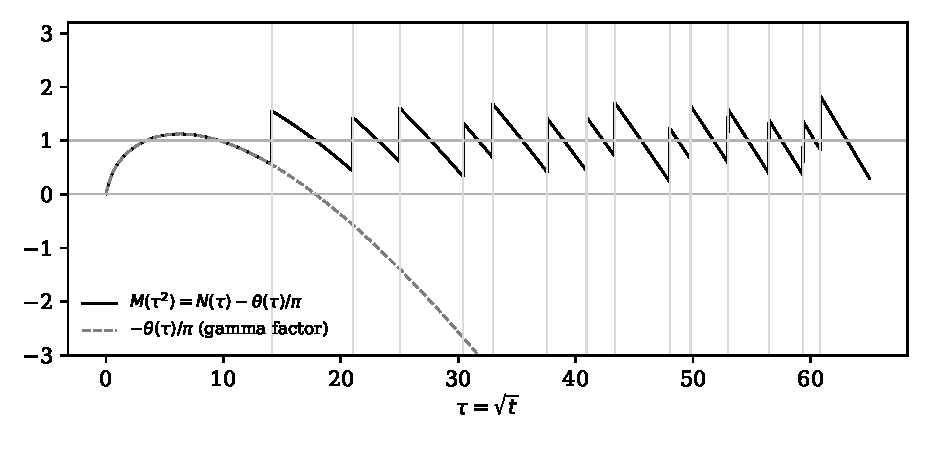
\includegraphics[width=0.9\textwidth]{rzfig/fig_M.pdf}
\caption{The function $M(\tau^2)=N(\tau)-\theta(\tau)/\pi=1+S(\tau)$ against $\tau=\sqrt t$, with the zero ordinates marked; under RH it is the distribution function of the Thorin measure of $\varphi$. The dashed curve is the gamma factor contribution $-\theta(\tau)/\pi$ alone. The function $M$ rises on $(0,\tau_0)$; beyond $\tau_0$, and so between consecutive ordinates, it decreases with slope $-\theta'(\tau)/\pi$, and at each ordinate it jumps by one. The mean level is $1$.}
\label{rz:fig:M}
\end{figure}

\subsection{L\'evy density, theta functions and a criterion for RH}\label{rz:sec:levy}

Under RH, integrating by parts in Theorem~\ref{rz:thm:thorin} and using $s/(s+t)=\int_0^\infty(1-e^{-sx})te^{-tx}dx$ turns the Thorin type representation of $\varphi$ into a L\'evy Khintchine one,
\begin{gather*}
\log\varphi(s)=-\int_0^\infty\bigl(1-e^{-sx}\bigr)\frac{w(x)}{x}\,dx,\\
w(x)=\int e^{-tx}\,dM(t),\qquad \frac{w(x)}{x}=\int_0^\infty e^{-tx}M(t)\,dt .
\end{gather*}
The function $w$, unlike $M$, can be written down without the zeros, and without RH.

\begin{theorem}\label{rz:thm:w}
Define, unconditionally,
\[
w(x)=e^{x/4}-P(x),\qquad P(x)=\frac{1}{\sqrt{4\pi x}}\sum_{n\ge2}\frac{\Lambda(n)}{\sqrt n}\,e^{-(\log n)^2/4x},\qquad x>0.
\]
Then $-\varphi'/\varphi(s)=\int_0^\infty e^{-sx}w(x)\,dx$ for $s>\frac14$, and for every $x>0$
\begin{equation}\label{rz:eq:weil}
\begin{gathered}
w(x)=W(x)-W_0(x),\qquad W(x)=\tfrac12\sum_\rho e^{x(\rho-\frac12)^2},\\
W_0(x)=\frac1\pi\int_0^\infty e^{-x\tau^2}\theta'(\tau)\,d\tau,
\end{gathered}
\end{equation}
the sum running over all nontrivial zeros with multiplicity. Here $W$ is the heat trace of Section~\ref{ch:clock} in the variable $x$; under RH, $W(x)=\sum_{\gamma>0}e^{-x\gamma^2}$ and $w(x)=\int e^{-tx}dM(t)$. The function $w$ satisfies $w(0^+)=1$ and $w(x)\sim c/(2\sqrt{\pi x})$ as $x\to\infty$.
\end{theorem}

\begin{proof}
By logarithmic differentiation, $-\varphi'/\varphi=\frac{1}{s-1/4}+\frac{1}{2\sqs}\frac{\zeta'}{\zeta}(\frac12+\sqs)$. The first term is the transform of $e^{x/4}$; for the second use $\zeta'/\zeta=-\sum\Lambda(n)n^{-z}$ and $\frac{1}{2\sqs}e^{-a\sqs}=\int_0^\infty e^{-sx}(4\pi x)^{-1/2}e^{-a^2/4x}dx$, with Tonelli justified on $s>\frac14$. Identity \eqref{rz:eq:weil} is Weil's explicit formula for the even test function $h(r)=e^{-xr^2}$, whose Fourier partner is $g(u)=(4\pi x)^{-1/2}e^{-u^2/4x}$: the pole contributes $h(\pm\frac i2)=e^{x/4}$, the archimedean place contributes $W_0$, and the primes contribute $P$. It is \eqref{eq:ch2:Warith} of Section~\ref{ch:clock} with $t=x$. Under RH, Theorem~\ref{rz:thm:thorin} gives the same Laplace transform for $\int e^{-tx}dM(t)$ and uniqueness identifies the two. The limit $w(0^+)=1$ holds because $P(x)=O(x^{-1/2}e^{-(\log2)^2/4x})$ as $x\to0$. The behaviour at infinity needs no hypothesis: every term of $W$ has modulus at most $e^{-x(\gamma^2-1/4)}$ with $\gamma>14$, so $W$ decays exponentially, while $W_0(x)\sim-c/(2\sqrt{\pi x})$ by Lemma~\ref{rz:lem:W0} below.
\end{proof}

We call $w$ the canonical function of $\varphi$: when $\varphi$ is infinitely divisible, $w(x)/x$ is its L\'evy density, and $\varphi$ is infinitely divisible exactly when $w\ge0$. Theorem~\ref{rz:thm:w} gives $w$ two faces. On the prime side $w$ is the heat trace $e^{x/4}=h(\pm\frac i2)$ of the pole, the Gaussian evaluated at the imaginary ordinate of $z=1$, minus the heat trace $P$ of the prime powers, each a Gaussian in $\log n$ of variance $2x$; this series converges absolutely for every $x>0$, which is the reason for working with the heat kernel $e^{-tx}$. On the zero side $w$ is the heat trace over the zeros minus that of their smooth count $\theta/\pi$, which comes from the gamma factor. The proof of Theorem~\ref{rz:thm:id} uses both faces, the prime side for small $x$ and the finitely many verified zeros for large $x$, and it rests on the following integral formula for $W_0$.

\begin{lemma}\label{rz:lem:W0}
For $x>0$,
\[
W_0(x)=\frac{F(x)}{4\sqrt{\pi x}},\qquad F(x)=2\theta'(0)+\int_0^\infty\frac{e^{-u/4}\bigl(1-e^{-u^2/16x}\bigr)}{1-e^{-u}}\,du .
\]
The function $F$ is strictly decreasing, $F(0^+)=+\infty$ and $F(\infty)=2\theta'(0)=\psi(\frac14)-\log\pi<0$. Hence $W_0$ has exactly one zero $x_*$, with $W_0>0$ on $(0,x_*)$ and $W_0<0$ on $(x_*,\infty)$.
\end{lemma}

\begin{proof}
Insert $\psi(z)=\int_0^\infty\bigl(e^{-u}/u-e^{-zu}/(1-e^{-u})\bigr)du$ with $z=\frac14+\frac{i\tau}2$ into $\theta'$, and use $\int_0^\infty e^{-x\tau^2}\cos(\tau u/2)\,d\tau=\frac12\sqrt{\pi/x}\,e^{-u^2/16x}$; the interchange is justified after writing the $\psi$ integrand as $e^{-u}/u-e^{-u/4}/(1-e^{-u})$ plus $e^{-u/4}(1-\cos(\tau u/2))/(1-e^{-u})$, both absolutely integrable against $e^{-x\tau^2}$. The terms free of $\tau$ reassemble into $\psi(\frac14)-\log\pi$. The integrand of $F$ is positive and decreasing in $x$; as $x\to0$ it increases to $e^{-u/4}/(1-e^{-u})$, which is not integrable at $0$.
\end{proof}

The Vere-Jones representation of Theorem~\ref{rz:thm:saw} writes $w$ as an absolutely convergent series of theta functions, one for each block. For the sawtooth measure of Lemma~\ref{rz:lem:saw} define its heat trace
\[
h_\lambda(x)=-\int e^{-tx}\,U_\lambda(dt)=\sum_{k\ge0}e^{-x\sigma_k(\lambda)}-\frac{\lambda}{4\sqrt{\pi x}}
=\frac{\lambda}{2\sqrt{\pi x}}\sum_{j\ge1}(-1)^je^{-j^2\lambda^2/4x},
\]
the last form by Poisson summation. The first form is a sum over the pseudo zeros minus their smooth count and the second a sum over the multiples $j\lambda$, so this Jacobi theta identity is the explicit formula of the toy zeta function $1+e^{-\lambda\sqs}$.

\begin{proposition}\label{rz:prop:theta}
For every $x>0$, with absolutely convergent sums,
\[
w(x)=e^{x/4}+\sum_{N\ge2}B_N\,h_{\log N}(x).
\]
\end{proposition}

\begin{proof}
Substitute the theta form of $h_\lambda$ and regroup the triple sum over $(n,m,j)$ by $r=mj$. The coefficient of $e^{-r^2(\log n)^2/4x}$ is
\[
-(4\pi x)^{-1/2}a_n\log n\sum_{mj=r}m\,d_m(-1)^{j+1},
\]
and the inner sum is $\delta_{r,1}$ because its Dirichlet series is $\eta(v)^{-1}\cdot\eta(v)$. Since $a_n\log n=\Lambda(n)/\sqrt n$ the sum equals $-P(x)$. The bound $|m\,d_m|\le m$ against Gaussian decay gives absolute convergence.
\end{proof}

Proposition~\ref{rz:prop:theta} is the Vere-Jones form of Theorem~\ref{rz:thm:w}. Unconditionally, $w$ is the Laplace transform, term by term, of the formal series $\delta_{-1/4}+\sum_NB_N\{\sum_k\delta_{\sigma_k(\log N)}-\frac{\log N}{4\pi\sqrt t}dt\}$ of sech atom lattices, with all the arithmetic in the weights $B_N$; under RH it is also the Laplace transform of $dM$. The atom at $-\frac14$ comes from the pole of $\zeta$ and lies outside $(0,\infty)$, where Thorin measures live, so under RH the sawtooth series must cancel it. Two consequences follow. The first makes the sawtooth expansion of $S$ rigorous after Gaussian averaging.

\begin{corollary}\label{rz:cor:Ssaw}
Assume RH. For every $x>0$,
\[
\int_0^\infty S(\tau)\,2\tau e^{-x\tau^2}\,d\tau=\frac{e^{x/4}-1}{x}+\sum_{N\ge2}B_N\int_0^\infty\Sigma_{\log N}(\tau)\,2\tau e^{-x\tau^2}\,d\tau,
\]
and each integral on the right equals $h_{\log N}(x)/x$.
\end{corollary}

\begin{proof}
By Theorem~\ref{rz:thm:w},
\[
\int_0^\infty e^{-tx}(1+S(\sqrt t))dt=w(x)/x,
\]
and $\int_0^\infty e^{-tx}\Sigma_\lambda(\sqrt t)\,dt=h_\lambda(x)/x$ by parts since $\Sigma_\lambda(0)=0$. Subtract $\int e^{-tx}dt=1/x$ and apply Proposition~\ref{rz:prop:theta}; substitute $t=\tau^2$.
\end{proof}

This is the sawtooth analogue of the classical formal series $S(\tau)=-\pi^{-1}\sum_na_n\sin(\tau\log n)$, with the pole appearing as the correction $(e^{x/4}-1)/x$. The second consequence is a criterion for RH.

\begin{theorem}\label{rz:thm:crit}
The following are equivalent.
\begin{enumerate}
\item[(i)] The Riemann Hypothesis.
\item[(ii)] There is a real signed Borel measure $m$ on $[0,\infty)$ with $\int|m|(dt)/(1+t)<\infty$ and $w(x)=\int e^{-tx}m(dt)$ for all $x>0$.
\end{enumerate}
In that case $m=dM$.
\end{theorem}

\begin{proof}
If RH holds take $m=dM$; the atoms satisfy $\sum(1+\gamma^2)^{-1}<\infty$ and the density is $O(t^{-1/2}(1+t)^{-1}\log(2+t))$ after division by $1+t$. Conversely, given $m$, put $J(s)=\int m(dt)/(s+t)$, analytic on $\cut$. For $s>\frac14$ Fubini gives $\int_0^\infty e^{-sx}w(x)dx=J(s)$, so $-\varphi'/\varphi=J$ on $(\frac14,\infty)$ and hence on all of $\cut$ by analytic continuation. A zero or pole of $\varphi$ in $\cut$ would be a pole of $-\varphi'/\varphi$, so $\varphi$ has none, and Proposition~\ref{rz:prop:rh} gives RH. Uniqueness of the Stieltjes transform gives $m=dM$.
\end{proof}

The criterion is a statement about $w$ alone, which is computable from the primes. In the language of Proposition~\ref{rz:prop:theta}, RH says that the formal measure $\delta_{-1/4}+\sum_NB_N(-U_{\log N})$ has the Laplace transform of a genuine real measure on $[0,\infty)$. If RH fails, a zero $\rho=\frac12+\beta+i\gamma$ with $\beta>0$ and its conjugate contribute to $W$ the term $e^{x(\beta^2-\gamma^2)}\cos(2\beta\gamma x)$, and the quadruple $\rho,\bar\rho,1-\rho,1-\bar\rho$ contributes twice this. The term is the real part of the Laplace transform of an atom at the complex point $(\gamma-i\beta)^2$, and no real measure on $[0,\infty)$ can reproduce it.

\subsection{Across the critical strip}\label{rz:sec:strip}

Moving the line of evaluation across the critical strip puts the results of this section and of Section~\ref{ch:rz3} in one picture. Fix $\sigma$ and evaluate $\zeta$ on the line $\Re z=\sigma$ through $z=\sigma+\sqs$. A zero $\rho=\beta+i\gamma$ then sits at $s=(\rho-\sigma)^2$: if $\beta>\sigma$ it gives a pole of $1/\zeta(\sigma+\sqs)$ in $\cut$, if $\beta=\sigma$ a point of the cut, and if $\beta<\sigma$ no singularity, only a Poisson kernel of width $\sigma-\beta$ in the Thorin density. On each line one can ask whether a normalised reciprocal of $\zeta$ is infinitely divisible, that is, has a L\'evy representation with positive L\'evy measure, and whether the completed function $R_\sigma(s)=\xi(\sigma)/\xi(\sigma+\sqs)$ has the stronger GGC property.

To the right of $\Re z=1$ the first question has a classical answer, in the variable $\tau$ rather than $s$. The Dirichlet series converges, $\zeta(\sigma+i\tau)/\zeta(\sigma)=\E e^{-i\tau\log N_\sigma}$ for the zeta distribution $\Pr(N_\sigma=n)=n^{-\sigma}/\zeta(\sigma)$, and the L\'evy measure of $\log N_\sigma$ is the prime measure $\sum_n\Lambda(n)n^{-\sigma}(\log n)^{-1}\delta_{\log n}$. The Vere-Jones representation writes this measure as a superposition of the alternating lattices $\sum_j(-1)^{j+1}j^{-1}\delta_{jn\log p}$, the signed L\'evy measures of fair coins, one for each prime power $p^n$, with weight the necklace polynomial $b_n(p^{-\sigma})$ (Theorem~\ref{rz:thm:necklace}). At $\sigma=0$ the weight $b_n(1)$ is $1$ when $n$ is a power of $2$ and $0$ otherwise, and the identity becomes Euler's binary product, with every block a solved model of unit multiplicity; for $\sigma>0$ the weights are fractional and some are negative.

Inside the strip $|\zeta(\sigma+i\tau)|$ is unbounded, while a characteristic function is bounded by $1$, so the characteristic function picture breaks down; the Vere-Jones representation survives in the variable $s$. For $0<\sigma<1$ put $\varphi_\sigma(s)=\zeta(\sigma)/\{(1-s/(1-\sigma)^2)\zeta(\sigma+\sqs)\}$, which is $\varphi$ at $\sigma=\frac12$. For $s>(1-\sigma)^2$, $-\varphi_\sigma'/\varphi_\sigma$ is the Laplace transform of a function $w_\sigma$, given by the theta series of Proposition~\ref{rz:prop:theta} (Section~\ref{rz:sec:levy}) with $e^{(1-\sigma)^2x}$ in place of $e^{x/4}$ and the weights $b_n(p^{-\sigma})$ in place of $B_{p^n}=b_n(p^{-1/2})$ (Theorem~\ref{rz:thm:levystrip}). When $w_\sigma\ge0$ this is a L\'evy representation, $\log\varphi_\sigma(s)=-\int(1-e^{-sx})w_\sigma(x)x^{-1}dx$, with an explicit L\'evy density built from the primes. Theorem~\ref{rz:thm:id} proves $w_{1/2}=w>0$, and numerically $w_\sigma>0$ on nine lines from $\sigma=0.05$ to $\sigma=0.99$, for $10^{-4}\le x\le10^3$ (Section~\ref{ch:rz3}); whether infinite divisibility holds on every line of the strip is open (Problem~\ref{rz:prob:strip}).

The Thorin property is where the zeros enter. The functions $\varphi_\sigma$ are never GGCs, for a reason that uses no information about $\zeta$: the factor removing the pole makes $w_\sigma$ increase at the origin (Proposition~\ref{rz:prop:onlyhalf}). For $\sigma\ge\frac12$, by Theorem~\ref{rz:thm:threshold}, the form of Theorem~\ref{thm:poisson} in the coordinates of Section~\ref{rz:sec:intro}, the function $R_\sigma$ is a GGC if and only if $\zeta(z)\ne0$ for $\Re z>\sigma$, and its Thorin measure is then the zero density smoothed by Poisson kernels of widths $\sigma-\beta$ in the variable $\sqrt t$. The smallest such $\sigma$ is $\Theta=\sup\Re\rho$, and RH is the statement $\Theta=\frac12$: the kernels then sharpen all the way to the unit atoms at $\gamma^2$ of the Thorin measure of $R$ (Proposition~\ref{prop:struct} and the paragraph after Theorem~\ref{rz:thm:threshold}). The Thorin density of the gamma factor is also built from Poisson kernels (Theorem~\ref{rz:thm:gamma}), but their widths $c_n=2n+\frac12$ are fixed and never sharpen, so the gamma factor produces no atoms. Table~\ref{rz:tab:strip} records the picture.

\begin{table}[htbp]
\centering
\small
\begin{tabular}{p{0.2\textwidth}p{0.34\textwidth}p{0.34\textwidth}}
\toprule
Line & L\'evy representation & Thorin representation of $R_\sigma$\\
\midrule
$\sigma>1$ & $\zeta(\sigma+i\tau)/\zeta(\sigma)=\E e^{-i\tau\log N_\sigma}$; prime L\'evy measure as a necklace weighted superposition of fair coin lattices & GGC, unconditionally; Thorin measure a Poisson smoothed zero density\\
$\sigma=1$ & not treated here & GGC, unconditionally; no atoms, since $\zeta$ has no zeros on $\Re z=1$\\
$\frac12<\sigma<1$ & $w_\sigma>0$ numerically & GGC if and only if there are no zeros with $\Re\rho>\sigma$\\
$\sigma=\frac12$ & $w>0$ proved & GGC if and only if RH; the Poisson kernels sharpen to atoms at $\gamma^2$\\
$\sigma<\frac12$ & $w_\sigma>0$ numerically & never: each zero on the critical line gives a pole of $R_\sigma$ in $\cut$\\
\bottomrule
\end{tabular}
\caption{The two questions across the critical strip. Middle column: the L\'evy representation, in the variable $\tau$ for $\sigma>1$ and in the heat kernel form of Theorem~\ref{rz:thm:levystrip} for $0<\sigma<1$, where the L\'evy measure is positive when $w_\sigma>0$. Right column: whether $R_\sigma$ is a GGC (Theorem~\ref{rz:thm:threshold}).}
\label{rz:tab:strip}
\end{table}

Chapters~\ref{chap:basepoint} to \ref{chap:almost} return to the completed functions $R_\sigma$, written there $\varphi_\alpha(u)=\xi(\alpha)/\xi(\alpha+\sqrt u)$, with the basepoint $\alpha$ in place of $\sigma$ and the variable $u$ of the book in place of $s$; they are not the normalised functions $\varphi_\sigma$ of this section. Section~\ref{ch:basepoint} studies the basepoint $\alpha=1$, the leftmost at which the GGC property is a theorem, Section~\ref{ch:strip} shows that $\xi(\alpha)/\xi(\alpha+|v|)$, as a function of real $v$, is the characteristic function of a normal scale mixture at every basepoint, and Section~\ref{ch:almost} shows by zero density estimates that for every $\alpha>\frac12$ the negative part of the Thorin measure up to height $T$, if there is one, is a vanishing proportion of the whole as $T\to\infty$.

\section{The gamma factor, the Meixner law and the sine squared lemma}\label{ch:rz2}

In Section~\ref{ch:rz1} the gamma factor $G$ entered through the factorisation $\varphi=RG$ and its Thorin density $-\theta'(\sqrt t)/(2\pi\sqrt t)$, which changes sign at $t=\tau_0^2$. Its Weierstrass product writes this density as a renormalised series of Poisson kernels of widths $c_n=2n+\frac12$, and adding it to Proposition~\ref{rz:prop:theta} gives the formal Thorin measure of the reciprocal Xi function $R$ in Vere-Jones form. On the critical line $|G|^2$ is proportional to the density of a Meixner hypergeometric law, whose characteristic function is a GGC transform in the square of its variable and whose orthogonal polynomials satisfy a local Riemann Hypothesis. The sine squared lemma turns the L\'evy measure of $\log f$ into the Thorin measure of $f(0)/f(\sqs)$. It shows that after a stable tilt the reciprocals of $\zeta(\beta+\sqs)$, for $\beta>1$, and of the gamma factor are GGC transforms, and it shows how positivity is lost at the centre. Section~\ref{rz:sec:floor} follows the tilt of the gamma factor to the floor $e^{-c\sqs}R$ of the reciprocal Xi function.

\subsection{The gamma factor in Vere-Jones form}\label{rz:sec:gamma}

Recall from Section~\ref{rz:sec:intro} the constants $c_n=2n+\frac12$ for $n\ge0$ and $b=\frac12(\gamma_E+\log\pi)\approx0.860973$, where $\gamma_E$ is Euler's constant. With these constants the Weierstrass product writes $G$ as a product of GGC transforms whose Thorin densities are Poisson kernels, renormalised by stable factors.

\begin{theorem}\label{rz:thm:gamma}
For $s\in\cut$,
\[
G(s)=e^{-b\sqs}\prod_{n\ge0}\frac{e^{\sqs/(2n+2)}}{1+\sqs/c_n},
\]
and the Thorin measure of $G$ is
\[
U_G(dt)=\frac{1}{2\pi\sqrt t}\Bigl\{b+\sum_{n\ge0}\Bigl(\frac{c_n}{t+c_n^2}-\frac{1}{2n+2}\Bigr)\Bigr\}dt=-\frac{\theta'(\sqrt t)}{2\pi\sqrt t}\,dt .
\]
Each factor $(1+\sqs/\kappa)^{-1}$ is the Laplace transform of a GGC, with positive Thorin density $q_\kappa(t)=\dfrac{\kappa}{2\pi\sqrt t\,(t+\kappa^2)}$, a Poisson kernel in $\sqrt t$; each factor $e^{a\sqs}$ with $a>0$ has the negative Thorin density $-a/(2\pi\sqrt t)$.
\end{theorem}

\begin{proof}
Weierstrass gives $\log\Gamma(z_0+v)-\log\Gamma(z_0)=-\gamma_Ev-\log(1+v/z_0)+\sum_{n\ge1}\{v/n-\log(1+v/(n+z_0))\}$. Take $z_0=\frac14$, $v=\sqs/2$, note $v/(n+\frac14)=\sqs/c_n$, and shift the index of $v/n$. For $q_\kappa$: $\frac{d}{ds}\log(1+\sqs/\kappa)=\frac{1}{2\sqs(\sqs+\kappa)}$, and Lemma~\ref{rz:lem:inv} with $\sqrt{-t+i0}=i\sqrt t$ gives the density $\frac{\kappa}{2\pi\sqrt t(t+\kappa^2)}$. For $e^{a\sqs}$ use $\int_0^\infty\log(1+s/t)t^{-1/2}dt=2\pi\sqs$. To sum the Thorin densities of the factors, write the bracket with index $n$ in $U_G$ as $(\frac1{c_n}-\frac1{2n+2})-\frac{t}{c_n(t+c_n^2)}$: both parts are nonnegative, and over $n$ the first sums to a constant and the second to $O(\log(2+t))$, so Tonelli's theorem applies to each part against $\log(1+s/t)\frac{dt}{2\pi\sqrt t}$ for $s>0$, and analytic continuation extends the sum to $\cut$; the same split justifies the termwise integration against $e^{-tx}$ in Proposition~\ref{rz:prop:W0erfc}. The identification with $\theta'$ is the partial fraction series $\Re\psi(\frac14+\frac{i\tau}2)=-\gamma_E+\sum_{n\ge0}\{\frac1{n+1}-\frac{2c_n}{c_n^2+\tau^2}\}$.
\end{proof}

Formally, the gamma factor is thus a renormalised infinite convolution of GGC laws, and the renormalisation is the only source of negativity in its Thorin density. Write $X_\varphi$ and $X_R$ for random variables with Laplace transforms $\varphi$ and $R$; both laws exist and are infinitely divisible, by Theorem~\ref{rz:thm:id} and by Theorem~\ref{thm:ch12:idsd} \cite[Theorem A]{P26}. Write $Y_\kappa$ for the variable with $\E e^{-sY_\kappa}=\kappa/(\kappa+\sqs)$, which is $Y_\kappa=E_\kappa^2/(4\Gamma_{1/2})$ with $E_\kappa$ exponential of rate $\kappa$ and $\Gamma_{1/2}$ an independent gamma variable of shape $\frac12$, and $L_a$ for the positive stable variable of index $\frac12$ with $\E e^{-sL_a}=e^{-a\sqs}$. Theorem~\ref{rz:thm:gamma} and Proposition~\ref{rz:prop:rh} then say formally
\begin{equation}\label{rz:eq:decon}
X_\varphi\;\overset{d}{=}\;X_R+L_b+\sum_{n\ge0}\bigl(Y_{c_n}\ominus L_{1/(2n+2)}\bigr),
\end{equation}
where $A\ominus B$ stands for a formal variable whose Laplace transform is the quotient of those of $A$ and $B$. Each bracket has Thorin density $\frac{1}{2\pi\sqrt t}\{\frac{c_n}{t+c_n^2}-\frac1{2n+2}\}$, positive for $t<\frac32c_n$ and negative beyond. The sum of the $Y_{c_n}$ diverges almost surely because $\sum1/c_n=\infty$, and the stable deconvolutions are the compensators that make the product of the Laplace transforms converge.

Figure~\ref{rz:fig:UG} shows the Thorin density of $G$ against the first three kernels. In the variable $\tau=\sqrt t$ it is $-\theta'(\tau)/\pi$, evaluated from the digamma function, so nothing in it depends on a zero of $\zeta$. It changes sign at the point $\tau_0$ where $\theta$ attains its minimum, so the reciprocal $1/G$ has a Thorin density that is negative near the origin, and $1/G$ becomes a GGC only after the stable tilt of Theorem~\ref{rz:thm:gammaggc}.

\begin{figure}[htbp]
\centering
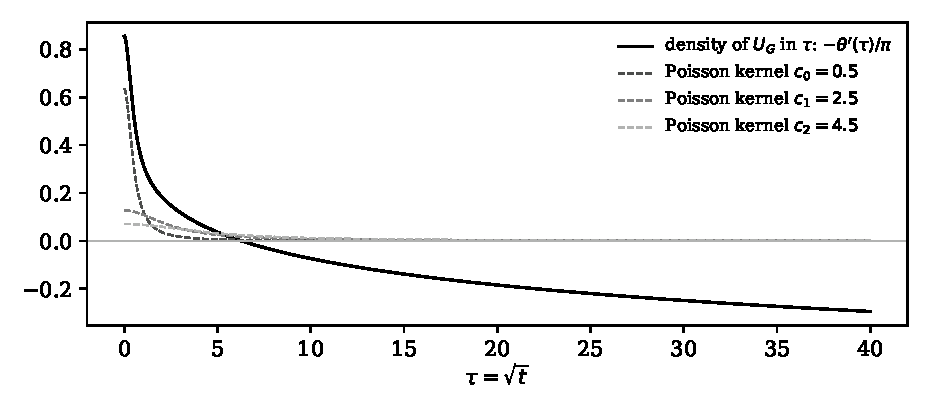
\includegraphics[width=0.9\textwidth]{rzfig/fig_UG.pdf}
\caption{The Thorin density of the gamma factor in the variable $\tau=\sqrt t$, namely $-\theta'(\tau)/\pi$, together with the first three Poisson kernels $c_n/(\pi(c_n^2+\tau^2))$ of Theorem~\ref{rz:thm:gamma}. The density is positive for $\tau<\tau_0\approx6.29$ and negative beyond, where the flat compensators outweigh the kernels.}
\label{rz:fig:UG}
\end{figure}

\begin{proposition}\label{rz:prop:W0erfc}
For $x>0$,
\[
W_0(x)=-\int e^{-tx}\,U_G(dt)=-\frac{b}{2\sqrt{\pi x}}+\sum_{n\ge0}\Bigl\{\frac{1}{(4n+4)\sqrt{\pi x}}-\frac12e^{c_n^2x}\operatorname{erfc}\bigl(c_n\sqrt x\bigr)\Bigr\}.
\]
\end{proposition}

\begin{proof}
$\int_0^\infty e^{-tx}q_\kappa(t)\,dt=\frac\kappa\pi\int_0^\infty\frac{e^{-xv^2}}{v^2+\kappa^2}dv=\frac12e^{\kappa^2x}\operatorname{erfc}(\kappa\sqrt x)$ and $\int_0^\infty e^{-tx}\frac{dt}{2\pi\sqrt t}=\frac{1}{2\sqrt{\pi x}}$.
\end{proof}

Both terms of the identity $W=w+W_0$ of \eqref{rz:eq:weil} are now explicit, and their sum is the heat trace over the zeros.

\begin{theorem}\label{rz:thm:RLVJ}
For every $x>0$, with absolutely convergent sums,
\begin{multline*}
W(x)=e^{x/4}+\sum_{N\ge2}B_N\,h_{\log N}(x)-\frac{b}{2\sqrt{\pi x}}\\
+\sum_{n\ge0}\Bigl\{\frac{1}{(4n+4)\sqrt{\pi x}}-\frac12e^{c_n^2x}\operatorname{erfc}\bigl(c_n\sqrt x\bigr)\Bigr\}.
\end{multline*}
Equivalently, $W(x)$ is the Laplace transform, taken term by term, of the formal series
\begin{multline*}
U_R=\delta_{-1/4}+\sum_{N\ge2}B_N\Bigl\{\sum_{k\ge0}\delta_{\sigma_k(\log N)}-\frac{\log N}{4\pi\sqrt t}\,dt\Bigr\}\\
-\frac{1}{2\pi\sqrt t}\Bigl\{b+\sum_{n\ge0}\Bigl(\frac{c_n}{t+c_n^2}-\frac1{2n+2}\Bigr)\Bigr\}dt ,
\end{multline*}
the formal Thorin measure of $R(s)=\xi(\frac12)/\xi(\frac12+\sqs)$. Under RH, $R$ is a GGC, and its Thorin measure $\sum_{\gamma>0}\delta_{\gamma^2}=dN(\sqrt t)$, where $N(T)$ counts the zeros with $0<\gamma\le T$, is a positive measure whose Laplace transform is also $W$.
\end{theorem}

\begin{proof}
$W=w+W_0$ by \eqref{rz:eq:weil}; substitute Proposition~\ref{rz:prop:theta} for $w$ and Proposition~\ref{rz:prop:W0erfc} for $W_0$. Term by term, $\delta_{-1/4}$ has Laplace transform $e^{x/4}$, the bracket with index $N$ has transform $h_{\log N}(x)$ by the definition of $h_\lambda$, and the last density is $-U_G$, whose transform is $W_0(x)$ by Proposition~\ref{rz:prop:W0erfc}. Under RH, Hadamard's product gives $R(s)=\prod_{\gamma>0}(1+s/\gamma^2)^{-1}$, as in the proof of Theorem~\ref{rz:thm:thorin}, and $W(x)=\sum_{\gamma>0}e^{-x\gamma^2}$ by Theorem~\ref{rz:thm:w}.
\end{proof}

The formula is the explicit formula for the heat trace in closed form: the polar term $e^{x/4}$, a sum over prime powers of the block theta functions $h_{\log N}$ weighted by the coefficients $B_N$ of Theorem~\ref{rz:thm:saw}, which Theorem~\ref{rz:thm:necklace} of Section~\ref{ch:rz3} expresses through necklace polynomials, and a sum of complementary error functions over the poles of the gamma factor. Each term is elementary and computable to high accuracy, and Table~\ref{rz:tab:num} checks the identity against the zero sum to twenty digits at $x=0.005$, $0.01$ and $0.03$.

In $U_R$ the pole gives an atom at $-\frac14$, off the half line $(0,\infty)$ that carries Thorin measures. The primes give lattices of sech atoms at $((2k+1)\pi/\log N)^2$, each compensated by its mean density. The gamma factor gives negative Poisson kernels of widths $c_n$ in the variable $\sqrt t$, with poles at $\sqrt t=\pm ic_n$, each compensated by a positive flat density. RH is the statement that the three groups combine into unit atoms at the $\gamma^2$ and nothing else. They combine only through Laplace transforms: every partial sum of $U_R$ carries the atom at $-\frac14$ and the Thorin measure $\sum_{\gamma>0}\delta_{\gamma^2}$ of $R$ under RH does not, so, like the series after Proposition~\ref{rz:prop:theta}, $U_R$ does not converge to that measure as a series of measures. By Theorem~\ref{rz:thm:crit}, $R$ has a Thorin type representation only if RH holds, since adding $U_G$ to its measure would give a measure $m$ as in condition (ii) there.

On the cut the gamma factor has modulus and phase
\[
G(-\tau^2+i0)=\frac{|\Gamma(\frac14+\frac{i\tau}2)|}{\Gamma(\frac14)}\,e^{i\theta(\tau)} .
\]
The phase is the Riemann Siegel theta function, and it is $-\pi$ times the distribution function of the Thorin measure: $U_G((0,\tau^2])=-\theta(\tau)/\pi$, since $\Im\log(1+s/t)=\pi$ for $t<\tau^2$ at $s=-\tau^2+i0$. The modulus is the logarithmic potential of the same measure,
\begin{equation}\label{rz:eq:pot}
\log\frac{|\Gamma(\frac14+\frac{i\tau}2)|}{\Gamma(\frac14)}=-\int\log\Bigl|1-\frac{\tau^2}{t}\Bigr|\,U_G(dt),
\end{equation}
the integral converging absolutely.

The square of the modulus is proportional to the density of a Meixner hypergeometric law, with parameter $a=\frac14$; Lai and Vere-Jones \cite{LVJ} study this family and its case $a=\frac12$, the hyperbolic secant law. Since $\int|\Gamma(a+ix)|^2e^{iux}dx=2\pi\Gamma(2a)(2\cosh\frac u2)^{-2a}$,
\begin{equation}\label{rz:eq:meixner}
p(\tau)=\frac{|\Gamma(\frac14+\frac{i\tau}2)|^2}{2^{3/2}\pi^{3/2}}\quad\text{is a probability density with}\quad\int p(\tau)e^{iv\tau}d\tau=\sech(v)^{1/2}.
\end{equation}
In this section $p$ denotes this Meixner density; the P\'olya density $\Phi/\Xi(0)$ of Section~\ref{ch:clock} does not occur. Since $\Xi(\tau)=-\frac12(\tau^2+\frac14)\pi^{-1/4}|\Gamma(\frac14+\frac{i\tau}2)|Z(\tau)$, with Hardy's function $Z(\tau)=e^{i\theta(\tau)}\zeta(\frac12+i\tau)$ of Section~\ref{ch:classical}, the Meixner density is the archimedean part of $\Xi^2$ on the critical line:
\[
\Xi(\tau)^2=\tfrac14\bigl(\tau^2+\tfrac14\bigr)^2\,2^{3/2}\pi\,p(\tau)\,Z(\tau)^2 .
\]
Lai and Vere-Jones call the Meixner hypergeometric distribution the odd man out; the characteristic function $\sech(v)^{1/2}$ of $p$ is a power of the kernel of Proposition~\ref{rz:prop:lvj}. We return to this law in Section~\ref{rz:sec:meixner}.

\subsection{From L\'evy to Thorin: the sine squared lemma}\label{rz:sec:sin2}

For a function of the form $f(0)/f(\sqs)$ we call $f$ its primal function. The sine squared lemma of \cite[Lemma 1]{P17v5} converts the L\'evy measure of $\log f$ into the Thorin measure of $f(0)/f(\sqs)$. The Vere-Jones representation produces such L\'evy measures, sums of atoms at the points $k\log N$, so the lemma applies to them. We state it in its original scaling and then in the coordinates of Section~\ref{rz:sec:intro}.

\begin{lemma}[{\cite[Lemma 1]{P17v5}}]\label{rz:lem:P1}
Suppose that for some measure $\mu$ on $(0,\infty)$ and some $\alpha$ with $\int_0^\infty(1\wedge x)e^{-\alpha x}\,\mu(dx)<\infty$,
\[
\log\frac{f(\alpha+s)}{f(\alpha)}-s\frac{f'(\alpha)}{f(\alpha)}=\int_0^\infty\bigl(e^{-sx}-1+sx\bigr)e^{-\alpha x}\,\frac{\mu(dx)}x,\qquad s\ge0 .
\]
Then, for $s\ge0$,
\[
\log\frac{f(\alpha)}{f(\alpha+s)}+s\frac{f'(\alpha)}{f(\alpha)}=-\int_0^\infty\bigl(1-e^{-\frac12s^2t}\bigr)\frac{\nu_\alpha(t)}t\,dt,
\]
\[
\nu_\alpha(t)=\frac{1}{\sqrt{2\pi}}\int_0^\infty e^{-tz}\Bigl\{\int_0^\infty2\sin^2\bigl(x\sqrt{z/2}\bigr)e^{-\alpha x}\,\mu(dx)\Bigr\}\frac{dz}{\sqrt{\pi z}} .
\]
The map $\mu\mapsto\nu_\alpha$ is linear and positivity preserving.
\end{lemma}

In these coordinates, with $s=u^2$ and $u=\sqs$, the lemma reads as follows. We include the proof by subordination, because its two stages, a L\'evy density in $s$ followed by a Thorin density, reappear in Section~\ref{rz:sec:floor}.

\begin{lemma}[Lemma~\ref{rz:lem:P1} in the scaling $s=u^2$]\label{rz:lem:sin2}
Let $\tilde\mu$ be a signed measure on $(0,\infty)$ with $\int(1\wedge x)|\tilde\mu|(dx)<\infty$, and suppose
\[
\log\frac{f(u)}{f(0)}-u\frac{f'(0)}{f(0)}=\int_0^\infty\bigl(e^{-ux}-1+ux\bigr)\frac{\tilde\mu(dx)}x,\qquad u\ge0 .
\]
Then for $s\in\cut$
\begin{gather*}
\log\frac{f(0)}{f(\sqs)}+\sqs\,\frac{f'(0)}{f(0)}=-\int_0^\infty\log\Bigl(1+\frac st\Bigr)U(t)\,dt,\\
U(t)=\frac{1}{2\pi\sqrt t}\int_0^\infty2\sin^2\Bigl(\frac{x\sqrt t}2\Bigr)\tilde\mu(dx).
\end{gather*}
If $\tilde\mu\ge0$ then $U\ge0$, and $s\mapsto f(0)e^{\sqs f'(0)/f(0)}/f(\sqs)$ is the Laplace transform of a GGC. Since $\sqs=\int\log(1+s/t)\,\frac{dt}{2\pi\sqrt t}$, the Thorin measure of $f(0)/f(\sqs)$ itself is $U(t)\,dt+\frac{f'(0)}{f(0)}\frac{dt}{2\pi\sqrt t}$.
\end{lemma}

\begin{proof}
Subordination by the first passage law \eqref{rz:eq:levy} gives, for $x,u>0$,
\[
e^{-ux}-1+ux=\int_0^\infty\bigl(1-e^{-u^2y}\bigr)\bigl(1-e^{-x^2/4y}\bigr)\frac{x}{\sqrt{4\pi y^3}}\,dy,
\]
because $\int_0^\infty(1-e^{-u^2y})\frac{x}{\sqrt{4\pi y^3}}dy=ux$. Integrating against $\tilde\mu(dx)/x$ gives a L\'evy form in $s=u^2$ with L\'evy density $k(y)/y$, where $k(y)=(4\pi y)^{-1/2}\int(1-e^{-x^2/4y})\tilde\mu(dx)$ is the canonical function. Finally $(1-e^{-x^2/4y})/\sqrt y=\int_0^\infty e^{-yt}\{1-\cos(x\sqrt t)\}\frac{dt}{\sqrt{\pi t}}$, so $k(y)=\int e^{-yt}U(t)dt$, and Frullani turns $\int(1-e^{-sy})k(y)\frac{dy}y$ into $\int\log(1+s/t)U(t)dt$. All kernels in these steps are nonnegative, so by Tonelli's theorem the steps hold with $|\tilde\mu|$ in place of $\tilde\mu$, and there every integral is finite, since $0\le(e^{-ux}-1+ux)/x\le\min(\frac{u^2x}2,u)$ and $\int(1\wedge x)|\tilde\mu|(dx)<\infty$; this justifies each interchange for the signed $\tilde\mu$. The analytic continuation to $\cut$ is immediate.
\end{proof}

Lemma~\ref{rz:lem:sin2} is \eqref{eq:sin2} of Section~\ref{ch:clock} integrated against $\tilde\mu(dx)/x$; the letters $s$ and $u$ are exchanged between the two sections. We call $\tilde\mu$ the primal L\'evy measure of $f(0)/f(\sqs)$. Positivity comes from the kernel. The signed cosine density that Lemma~\ref{rz:lem:inv} produces for a single exponential in an exponent (Section~\ref{rz:sec:prelim}) is $-\cos=2\sin^2-1$, and Lemma~\ref{rz:lem:sin2} separates it into the positive part $2\sin^2$ and a flat part $-1$, which is absorbed into the linear tilt $u\,f'(0)/f(0)$, a stable law of index $\frac12$.

\subsubsection{Zeta to the right of the line, the Vere-Jones blocks and the centre}

Where the primal L\'evy measure is positive the lemma applies directly. The first such case is $\zeta$ to the right of $\Re z=1$.

\begin{proposition}\label{rz:prop:zetaright}
For $\beta>1$ put $\tilde\mu_\beta=\sum_{n\ge2}\Lambda(n)n^{-\beta}\delta_{\log n}$. Then
\[
\frac{\zeta(\beta)}{\zeta(\beta+\sqs)}\,e^{\sqs\,\zeta'(\beta)/\zeta(\beta)}
=\exp\Bigl(-\int_0^\infty\log\Bigl(1+\frac st\Bigr)U_\beta(t)\,dt\Bigr),
\]
\[
U_\beta(t)=\frac{1}{2\pi\sqrt t}\sum_{n\ge2}\frac{\Lambda(n)}{n^\beta}\,2\sin^2\Bigl(\frac{\sqrt t\log n}2\Bigr)\ge0,
\]
so the left side is the Laplace transform of a GGC. Adding the tilt, the Thorin measure of $\zeta(\beta)/\zeta(\beta+\sqs)$ is $-\frac{1}{2\pi\sqrt t}\sum\Lambda(n)n^{-\beta}\cos(\sqrt t\log n)\,dt$, which is the Euler product density \eqref{rz:eq:formal} at $\beta$ in place of $\frac12$.
\end{proposition}

\begin{proof}
$\log\zeta(\beta+u)=\sum\Lambda(n)n^{-\beta}e^{-u\log n}/\log n$, so the hypothesis of Lemma~\ref{rz:lem:sin2} holds with $\tilde\mu_\beta$, which has finite mass for $\beta>1$.
\end{proof}

The tilt is needed: without it the Thorin density
\[
-\frac{1}{2\pi\sqrt t}\sum\Lambda(n)n^{-\beta}\cos(\sqrt t\log n)
\]
is negative near $t=0$. For $\xi$ no tilt is needed, since $s\mapsto\xi(\alpha)/\xi(\alpha+\sqs)$ is a GGC transform for every $\alpha\ge1$ (Theorem~\ref{thm:poisson}); at $\alpha=1$, Section~\ref{ch:basepoint} obtains its Thorin density from a L\'evy form of $\log\xi(1+u)$ by the same lemma. As $\beta\downarrow1$ the mass $\sum\Lambda(n)n^{-\beta}$ diverges, and at $\beta=\frac12$, where the pole and the gamma factor also enter, the lemma cannot be applied as it stands. The rest of this chapter and Chapter~\ref{chap:rzid} try to extend the case $\beta>1$ towards the critical line.

The Vere-Jones blocks have signed primal L\'evy measures, yet the lemma still gives positive Thorin densities. Apply it to one block $f_\lambda(u)=1+e^{-\lambda u}$ of Theorem~\ref{rz:thm:saw}, shifted by $\alpha>0$. Since $\log(1+e^{-\lambda(\alpha+u)})=\sum_k(-1)^{k+1}q^ke^{-k\lambda u}/k$ with $q=e^{-\lambda\alpha}$, the primal L\'evy measure is the alternating lattice $\tilde\mu_{\lambda,\alpha}=\lambda\sum_{k\ge1}(-1)^{k+1}q^k\delta_{k\lambda}$.

\begin{proposition}\label{rz:prop:block}
For $\alpha>0$ the sine squared transform of $\tilde\mu_{\lambda,\alpha}$ is positive:
\[
U_{\lambda,\alpha}(t)=\frac{\lambda}{2\pi\sqrt t}\,\frac{q(1-q)\bigl(1-\cos\lambda\sqrt t\bigr)}{(1+q)\bigl(1+2q\cos\lambda\sqrt t+q^2\bigr)}\ge0,
\]
so $\frac{1+e^{-\lambda\alpha}}{1+e^{-\lambda(\alpha+\sqs)}}\,e^{-\sqs\lambda q/(1+q)}$ is the Laplace transform of a GGC. As $\alpha\downarrow0$, $U_{\lambda,\alpha}(t)\,dt\to\sum_{k\ge0}\delta_{\sigma_k(\lambda)}$ vaguely, the tilt density tends to $-\frac{\lambda}{4\pi\sqrt t}$, and the Thorin measure of $2/(1+e^{-\lambda\sqs})$ is recovered as $\sum_k\delta_{\sigma_k(\lambda)}-\frac{\lambda}{4\pi\sqrt t}dt=-U_\lambda$, the sawtooth measure of Lemma~\ref{rz:lem:saw}.
\end{proposition}

\begin{proof}
$\sum_k(-1)^{k+1}q^k=\frac q{1+q}$ and $\sum_k(-1)^{k+1}q^k\cos k\omega=\frac{q\cos\omega+q^2}{1+2q\cos\omega+q^2}$; their difference is $\frac{q(1-q)(1-\cos\omega)}{(1+q)(1+2q\cos\omega+q^2)}\ge0$. As $q\uparrow1$ this is a Poisson kernel in $\omega=\lambda\sqrt t$ concentrating at $\omega=(2k+1)\pi$ with mass $\pi$ per period, which becomes $\sum_k\delta_{\sigma_k(\lambda)}$ after the change of variable. The tilt is $f'(\alpha)/f(\alpha)=-\lambda q/(1+q)\to-\lambda/2$.
\end{proof}

The sine squared image of each block is a Poisson kernel in $\sqrt t$ for $\alpha>0$ and the sech lattice at $\alpha=0$, so the negative part of the sawtooth measure is entirely the tilt. Summing the blocks with the weights $B_N$ gives $\log\zeta(\frac12+\alpha+\sqs)$, and the sum of Thorin densities $\sum_NB_NU_{\log N,\alpha}$ converges absolutely for $\alpha>\frac12$, where it equals $U_{1/2+\alpha}$ of Proposition~\ref{rz:prop:zetaright}. Positivity is then visible termwise in the prime form. It is not visible blockwise in the Vere-Jones form, because infinitely many weights are negative: $B_{p^3}=\frac13(p^{-3/2}-p^{-1/2})<0$ for every prime $p$, and Proposition~\ref{rz:prop:signs} of Section~\ref{ch:rz3} gives infinitely many more.

At $\beta=\frac12$ the prime L\'evy measure $\tilde\mu_{1/2}=\sum\Lambda(n)n^{-1/2}\delta_{\log n}$ has infinite mass, and both the image and the tilt in Lemma~\ref{rz:lem:sin2} diverge: the positive sine squared image has density of order $\frac{1}{2\pi\sqrt t}\sum\Lambda(n)n^{-1/2}=\infty$, and the tilt $\zeta'/\zeta(\frac12+0)$ is $-\infty$ along the Dirichlet series. The divergences cancel, and the heat trace makes the cancellation exact. Since $\int_0^\infty e^{-xt}\,2\sin^2(\frac{\sqrt t L}2)\frac{dt}{2\pi\sqrt t}=\frac{1-e^{-L^2/4x}}{2\sqrt{\pi x}}$, the heat trace of the sine squared image is formally
\[
\frac{1}{2\sqrt{\pi x}}\sum_{n\ge2}\frac{\Lambda(n)}{\sqrt n}\bigl(1-e^{-(\log n)^2/4x}\bigr)=\frac{1}{2\sqrt{\pi x}}\sum_{n\ge2}\frac{\Lambda(n)}{\sqrt n}-P(x).
\]
Replace the divergent constant by its analytic continuation $\sum\Lambda(n)n^{-1/2}\to-\zeta'(\frac12)/\zeta(\frac12)=-c$, and add the tilt $\frac{c}{2\sqrt{\pi x}}$ (the heat trace of $\frac{c}{2\pi\sqrt t}dt$) and the heat trace $e^{x/4}$ of the pole atom $\delta_{-1/4}$. The result is $e^{x/4}-P(x)=w(x)$, in agreement with Theorem~\ref{rz:thm:w}. So at the centre Lemma~\ref{rz:lem:sin2} still produces the correct Thorin measure $dM$, but only after a regularisation that subtracts an infinite positive constant from a positive density, and that is where the sign of $dM$ is lost.

\subsubsection{The inverse direction: cosine L\'evy forms}

The Frullani identity behind Lemma~\ref{rz:lem:sin2} also runs in the opposite direction, from a Thorin measure in $s$ to a symmetric L\'evy measure in $u=\sqs$: for $\beta>0$ and real $u$, $\int_0^\infty2\sin^2(\frac{ux}2)e^{-\beta x}\frac{dx}x=\frac12\log(1+u^2/\beta^2)$, hence
\begin{equation}\label{rz:eq:cosdict}
\int\log\Bigl(1+\frac st\Bigr)U(dt)=\int_0^\infty2\sin^2\Bigl(\frac{ux}2\Bigr)K_U(x)\,\frac{dx}x,\qquad K_U(x)=2\int e^{-\sqrt t\,x}\,U(dt).
\end{equation}
If $U\ge0$ then $u\mapsto\exp(-\int\log(1+u^2/t)U(dt))$ is the characteristic function of a symmetric infinitely divisible law with L\'evy density $K_U(|x|)/(2|x|)$. Section~\ref{ch:strip} applies this dictionary to $\xi(\alpha)/\xi(\alpha+|u|)$, which is the characteristic function of a normal scale mixture at every basepoint $\alpha$.

\begin{proposition}\label{rz:prop:dict}
Under \eqref{rz:eq:cosdict}:
\begin{enumerate}
\item[(i)] the Meixner law \eqref{rz:eq:meixner} has L\'evy density $\dfrac{1}{4|x|\sinh(\pi|x|/2)}$ on $\R$, and its characteristic function, as a function of $v^2$, is a GGC transform with Thorin measure $\frac12\sum_{k\ge0}\delta_{((k+1/2)\pi)^2}$, since $\sech(v)^{1/2}=\prod_k(1+v^2/((k+\frac12)\pi)^2)^{-1/2}$;
\item[(ii)] the sawtooth measure has $K_{U_\lambda}(x)=\dfrac{\lambda}{\pi x}-\dfrac{1}{\sinh(\pi x/\lambda)}$;
\item[(iii)] under RH, the Thorin measure $U=\sum_{\gamma>0}\delta_{\gamma^2}$ of $R$ has $K_U(x)=2\sum_{\gamma>0}e^{-\gamma x}$, Cram\'er's function \cite[Chapter I]{Cramer19}, and $\xi(\frac12)/\xi(\frac12+u)$ is the characteristic function of a sum of independent Laplace variables of scales $1/\gamma$.
\end{enumerate}
\end{proposition}

\begin{proposition}\label{rz:prop:diverge}
For every $x>0$ the series $\sum_NB_N\,K_{U_{\log N}}(x)$ diverges.
\end{proposition}

\begin{proof}
$B_N$ vanishes unless $N$ is a prime power. Grouping the powers of a fixed $p$, $\sum_kB_{p^k}/k=\sum_{j,m}d_m\,p^{-j/2}/(j^2m)=\frac{12}{\pi^2}p^{-1/2}+O(p^{-1})$, using $\sum_md_m/m=1/\eta(2)=12/\pi^2$. Since $K_{U_\lambda}(x)=\frac{\pi x}{6\lambda}+O((x/\lambda)^3)$, the group for $p$ equals $\frac{2x}{\pi}\frac{p^{-1/2}}{\log p}(1+o(1))$, and $\sum_pp^{-1/2}/\log p=\infty$. The grouping changes the order of summation, but in the order of increasing $N$ the partial sums are dominated by the prime terms $B_pK_{U_{\log p}}(x)\sim\frac{\pi x}{6}\frac{p^{-1/2}}{\log p}$, so the series diverges in that order as well.
\end{proof}

The inverse direction fails to sum over primes for the reason that Lemma~\ref{rz:lem:sin2} fails at the centre: without Gaussian damping the weights $p^{-1/2}$ are not summable. The Poisson kernel $e^{-\sqrt t\,x}$ is the stable $\frac12$ average of the heat kernel, $e^{-\sqrt t\,x}=\int_0^\infty e^{-ty}\frac{x}{2\sqrt\pi}y^{-3/2}e^{-x^2/4y}dy$, and the average extends over $y\gtrsim(\log N)^2$, where the block heat trace $h_{\log N}(y)$ has lost its Gaussian factor $e^{-(\log N)^2/4y}$ and is close to $-\log N/(4\sqrt{\pi y})$; each prime then contributes of order $p^{-1/2}/\log p$, as in the proof of Proposition~\ref{rz:prop:diverge}. Under the heat kernel alone each block heat trace is a theta function with Gaussian decay in $\log N$, and the series converges (Proposition~\ref{rz:prop:theta}, Theorem~\ref{rz:thm:RLVJ}).

\subsection{The Meixner law and its orthogonal polynomials}\label{rz:sec:meixner}

The Meixner hypergeometric law of Section~\ref{rz:sec:gamma}, whose density $p$ is proportional to $|G|^2$ on the critical line, is Brownian motion run for an independent GGC time. The score $-p'/p$ of the law and the derivative of the Riemann Siegel theta function are the imaginary and real parts of the boundary values of one Bernstein function, and the positivity of the L\'evy measure of that function makes the tilted reciprocal gamma factor a GGC. The orthogonal polynomials of the law are the Meixner Pollaczek polynomials. They give the local Riemann Hypothesis at the archimedean place and two expansions of $\zeta$ on the critical line, whose zeros we compare with the ordinates. Finally the law splits the autocorrelation of the P\'olya kernel into a Meixner factor and an arithmetic factor.

Let $Y$ have the density $p$ of \eqref{rz:eq:meixner}, so that $\E e^{ivY}=\sech(v)^{1/2}$.

\begin{proposition}\label{rz:prop:meixstruct}
\begin{enumerate}
\item[(i)] $Y\overset d=B(T)$, where $B$ is a standard Brownian motion and $T$ is independent with $\E e^{-\lambda T}=\sech(\sqrt{2\lambda})^{1/2}$, the variable $C_{1/2}$ of Biane, Pitman and Yor \cite{BPY01}, so that $Y$ is the value at time $\frac12$ of the process $\widehat C_t=B(C_t)$ of Pitman and Yor \cite[(1) and (4)]{PitmanYor03}. The time $T=\sum_{k\ge0}\frac{8\,\Gamma_k}{(2k+1)^2\pi^2}$, with $\Gamma_k$ independent gamma variables of shape $\frac12$ and unit scale, is a GGC with Thorin measure $\frac12\sum_k\delta_{(k+1/2)^2\pi^2/2}$.
\item[(ii)] $Y$ is infinitely divisible with L\'evy density $\dfrac{1}{4|x|\sinh(\pi|x|/2)}$, one half of the L\'evy density $1/(2|x|\sinh(\pi|x|/2))$ of the process $\widehat C$ \cite[Table~5]{PitmanYor03}; $Y$ has a Meixner law \cite{SchoutensTeugels98,Grigelionis99}. As $|\tau|\to\infty$, $p(\tau)\sim\pi^{-1/2}|\tau|^{-1/2}e^{-\pi|\tau|/2}$, matching the singularities of $\sech(v)^{1/2}$ at $v=\pm i\pi/2$.
\item[(iii)] $p$ is not a P\'olya frequency function of infinite order.
\end{enumerate}
\end{proposition}

\begin{proof}
(i) $\E e^{ivB(T)}=\E e^{-v^2T/2}=\sech(v)^{1/2}$, and $\sech(\sqrt{2\lambda})^{1/2}=\prod_k(1+2\lambda/((k+\frac12)\pi)^2)^{-1/2}$. (ii) is Proposition~\ref{rz:prop:dict}(i); the tail follows from Stirling, $|\Gamma(\frac14+ix)|^2\sim2\pi|x|^{-1/2}e^{-\pi|x|}$ with $x=\tau/2$. (iii) By Schoenberg's theorem \cite[Theorem 1]{Schoenberg51} the bilateral Laplace transform of a PF$_\infty$ density is the reciprocal of an entire function of Laguerre P\'olya class, so the reciprocal of its characteristic function is entire. Here $1/\E e^{ivY}=\cosh(v)^{1/2}$, which has branch points at the simple zeros $v=i(k+\frac12)\pi$ of $\cosh$ and is not entire.
\end{proof}

The time $T$ of (i), which is not the clock variable of Section~\ref{ch:clock}, is twice the Meixner time of Table~\ref{tab:ch3:cat}. The exponent $\frac12$ in $\sech(v)^{1/2}$ is the Meixner parameter $2a=\frac12$, forced by the factor $\Gamma(z/2)$ of $\xi$ at $z=\frac12$. For $2a$ a positive integer the Meixner law is PF$_\infty$; the zeta function sits at a value where it is not, although its characteristic function is still a GGC transform in $v^2$. This matters because P\'olya's approach to RH through the kernel of $\Xi$ is an approach through total positivity, and the archimedean factor alone already fails its strongest form.

Define the measure $\nu$ on $(0,\infty)$ by
\[
\nu(dy)=\frac{e^{y/2}}{\sinh y}\,dy=2\sum_{k\ge0}e^{-c_ky}\,dy ,
\]
with $c_k=2k+\frac12$ as in Theorem~\ref{rz:thm:gamma}. Its density is completely monotone, the Laplace transform of $2\sum_k\delta_{c_k}$, whose atoms sit at the points $c_k$ of the Weierstrass product of $G$.

\begin{proposition}\label{rz:prop:bernstein}
The function $\Phi_\Gamma(\lambda)=\psi(\frac14+\frac\lambda2)-\psi(\frac14)=\int_0^\infty(1-e^{-\lambda y})\,\nu(dy)$ is a Bernstein function. Its boundary values on the imaginary axis are
\[
\Re\Phi_\Gamma(i\tau)=2\bigl(\theta'(\tau)-\theta'(0)\bigr)=\int_0^\infty(1-\cos\tau y)\,\nu(dy),
\]
\[
\Im\Phi_\Gamma(i\tau)=-\frac{d}{d\tau}\log p(\tau)=\int_0^\infty\sin(\tau y)\,\nu(dy).
\]
Consequently $2\theta(\tau)+\tau\log\pi$ and $\log p(\tau)$ are, up to constants, the imaginary and real parts of $2\log\Gamma(\frac14+\frac{i\tau}2)$, the boundary value of a function analytic in the right half plane. So $2\theta(\tau)+\tau\log\pi$, which is $2\pi$ times the smooth part $\theta/\pi$ of the zero counting function plus a linear term, is the harmonic conjugate of the Meixner log density. The smooth heat trace is the heat trace of $\nu$:
\[
W_0(x)=\frac{\theta'(0)}{2\sqrt{\pi x}}+\frac{1}{4\sqrt{\pi x}}\int_0^\infty\bigl(1-e^{-y^2/4x}\bigr)\,\nu(dy),
\]
which is Lemma~\ref{rz:lem:W0} after the substitution $u=2y$; the function $F$ of that lemma decreases because $\nu$ is positive.
\end{proposition}

\begin{proof}
Substitute $u=2y$ in $\psi(z)=\int_0^\infty(e^{-u}/u-e^{-zu}/(1-e^{-u}))du$ with $z=\frac14+\frac\lambda2$; note $2e^{-y/2}/(1-e^{-2y})=e^{y/2}/\sinh y$. Taking $\lambda=i\tau$ gives the boundary values, with $\theta'=\frac12\Re\psi(\frac14+\frac{i\tau}2)-\frac12\log\pi$ and $\frac{d}{d\tau}\log|\Gamma(\frac14+\frac{i\tau}2)|^2=-\Im\psi(\frac14+\frac{i\tau}2)$. For $W_0$ integrate $\theta'(\tau)=\theta'(0)+\frac12\int(1-\cos\tau y)\nu(dy)$ against $\frac1\pi e^{-x\tau^2}$.
\end{proof}

Figure~\ref{rz:fig:meixner} shows the density and $\Phi_\Gamma(i\tau)$, evaluated from $\Gamma$ and $\psi$ alone, so the increment $\theta'(\tau)-\theta'(0)$, which is $\pi$ times the increase of the smooth zero density $\theta'/\pi$, appears with no zero as input.

\begin{figure}[htbp]
\centering
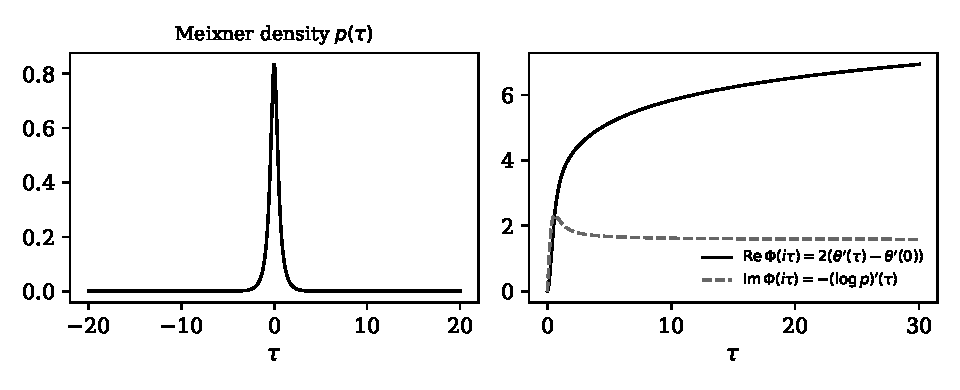
\includegraphics[width=0.95\textwidth]{rzfig/fig_meixner.pdf}
\caption{Left: the Meixner density $p(\tau)\propto|\Gamma(\frac14+\frac{i\tau}2)|^2$. Right: the real and imaginary parts of the Bernstein function $\Phi_\Gamma(i\tau)$ of Proposition~\ref{rz:prop:bernstein}, written $\Phi(i\tau)$ in the legend. The real part is $2(\theta'(\tau)-\theta'(0))$ and grows like $\log\tau$; the imaginary part is the Meixner score $-\frac{d}{d\tau}\log p$ and tends to $\pi/2$, the exponential tail rate of $p$.}
\label{rz:fig:meixner}
\end{figure}

\begin{theorem}\label{rz:thm:gammaggc}
Let $c=-\theta'(0)=\frac12(\log\pi-\psi(\frac14))\approx2.68609$ be the constant of \eqref{rz:eq:c}. Then
\[
\frac{e^{-c\sqs}}{G(s)}=\frac{\Gamma(\frac14)\,\pi^{\sqs/2}\,e^{-c\sqs}}{\Gamma(\frac14+\frac\sqs2)}=\exp\Bigl(-\int_0^\infty\log\Bigl(1+\frac st\Bigr)U_\Gamma(t)\,dt\Bigr),
\]
with
\[
U_\Gamma(t)=\frac{\theta'(\sqrt t)-\theta'(0)}{2\pi\sqrt t}=\frac{1}{2\pi\sqrt t}\sum_{k\ge0}\frac{t}{c_k\,(c_k^2+t)}\ge0 .
\]
So $e^{-c\sqs}/G(s)$ is the Laplace transform of a GGC, and its Thorin distribution function is $(\theta(\sqrt t)-\theta'(0)\sqrt t)/\pi$, a convex increasing function of $\sqrt t$.
\end{theorem}

\begin{proof}
With $f(u)=\Gamma(\frac14+\frac u2)\pi^{-u/2}$ we have $f'(0)/f(0)=\frac12\psi(\frac14)-\frac12\log\pi=\theta'(0)=-c$, and $\frac{d}{du}[\log f(u)-uf'(0)/f(0)]=\frac12\Phi_\Gamma(u)=\frac12\int(1-e^{-uy})\nu(dy)$. Integrating from $0$, $\log f(u)/f(0)-uf'(0)/f(0)=\int(e^{-uy}-1+uy)\frac{\tilde\mu(dy)}{y}$ with $\tilde\mu=\frac12\nu\ge0$. Lemma~\ref{rz:lem:sin2} gives $U_\Gamma(t)=\frac{1}{2\pi\sqrt t}\int2\sin^2(\frac{y\sqrt t}2)\frac12\nu(dy)=\frac{1}{2\pi\sqrt t}\sum_k\int_0^\infty(1-\cos y\sqrt t)e^{-c_ky}dy$, which is the series stated, and Proposition~\ref{rz:prop:bernstein} identifies it with $\theta'$.
\end{proof}

Multiplying $1/G$ by $e^{-c\sqs}$ adds the Thorin density $\frac{c}{2\pi\sqrt t}$, and $U_\Gamma=-U_G+\frac{c}{2\pi\sqrt t}$, which is the identity $c-b=\sum_k(\frac1{c_k}-\frac1{2k+2})$, has no negative part. This is the positive counterpart of Theorem~\ref{rz:thm:gamma}, where the gamma factor appeared as a renormalised product with a signed Thorin density: the archimedean factor becomes positive after one explicit tilt, which leaves the zeros as the only possible source of negativity in the floor of Section~\ref{rz:sec:floor}.

\subsubsection{Meixner Pollaczek polynomials and the local Riemann Hypothesis}

The Meixner law is also the orthogonality measure of the Meixner Pollaczek polynomials, and through them it controls the zeros of the Mellin transforms of the even Hermite functions. Let $\psi_{2m}(x)=H_{2m}(\sqrt{2\pi}\,x)e^{-\pi x^2}$ be the even Hermite functions, eigenfunctions of the Fourier transform $\hat f(y)=\int f(x)e^{-2\pi ixy}dx$ with eigenvalue $(-1)^m$. Define the Mellin transform $\mathcal Mf(s)=\int_0^\infty x^{s-1}f(x)dx$ and $\Gamma_{\R}(s)=\pi^{-s/2}\Gamma(s/2)$. From here to the end of Section~\ref{rz:sec:meixner}, $s$ is the Mellin variable, the argument of $\zeta$, and not the variable of the clock.

\begin{theorem}\label{rz:thm:localRH}
For each $m\ge0$, $Q_m(s)=\mathcal M\psi_{2m}(s)/\Gamma_{\R}(s)$ is a polynomial of degree $m$ satisfying $Q_m(1-s)=(-1)^mQ_m(s)$, and
\[
Q_m(\tfrac12+i\tau)=\kappa_m\,P_m^{(1/4)}\bigl(\tfrac\tau2;\tfrac\pi2\bigr),
\]
where $P_m^{(\lambda)}(x;\phi)$ are the Meixner Pollaczek polynomials and $\kappa_m\ne0$. These are the orthogonal polynomials of the Meixner law $p$. Consequently all zeros of $Q_m$ lie on $\Re s=\frac12$ and are simple: the Mellin transform of every even Hermite function satisfies the Riemann Hypothesis.
\end{theorem}

\begin{proof}
Expanding $H_{2m}(\sqrt{2\pi}\,x)=\sum_jh_jx^{2j}$ gives
\[
\mathcal M\psi_{2m}(s)=\frac12\Gamma_{\R}(s)\sum_jh_j\pi^{-j}(s/2)_j
\]
with Pochhammer symbols, a polynomial of degree $m$ times $\Gamma_{\R}(s)$. Tate's local functional equation \cite[Theorem 2.4.1 and Section 2.5]{Tate67}, $\mathcal Mf(s)/\Gamma_{\R}(s)=\mathcal M\hat f(1-s)/\Gamma_{\R}(1-s)$ for even $f$, applied to the eigenfunction $\psi_{2m}$ gives $Q_m(1-s)=(-1)^mQ_m(s)$, so $i^{-m}Q_m(\frac12+i\tau)$ is a real polynomial $R_m(\tau)$. By Mellin Plancherel,
\[
\int_0^\infty\psi_{2m}\psi_{2n}\,dx=\frac1{2\pi}\int_{\R}Q_m\overline{Q_n}\,|\Gamma_{\R}(\tfrac12+i\tau)|^2d\tau=\sqrt2\,i^{m-n}\int_\R R_m(\tau)R_n(\tau)\,p(\tau)\,d\tau,
\]
since $|\Gamma_{\R}(\frac12+i\tau)|^2=\pi^{-1/2}|\Gamma(\frac14+\frac{i\tau}2)|^2=2^{3/2}\pi\,p(\tau)$. The left side vanishes for $m\ne n$, so $(R_m)$ is the orthogonal polynomial sequence of $p$, which with $x=\tau/2$ is the Meixner Pollaczek family with $\lambda=\frac14$, $\phi=\frac\pi2$ \cite[Section 9.7]{KLS}. Orthogonal polynomials of a measure with infinite support have real simple zeros.
\end{proof}

The conclusion is the archimedean local Riemann Hypothesis of Bump, Choi, Kurlberg and Vaaler \cite{BCKV}, seen through the Meixner law: the squared modulus of the archimedean factor on the line, $|\Gamma_{\R}(\frac12+i\tau)|^2=2^{3/2}\pi\,p(\tau)$, is the orthogonality measure, and orthogonality forces the zeros of these Mellin transforms onto the line. We make no priority claim for this route; Meixner Pollaczek expansions of $\Xi$ in the literature are reviewed in Section~\ref{rz:sec:mpexp}. We checked numerically that the roots of $Q_m$ have real part $\frac12$ to 50 digits for $m\le8$, and that $Q_m(\frac12+i\tau)/P_m^{(1/4)}(\tau/2;\pi/2)$ is constant, with $\kappa_2=-16$, $\kappa_3=-192i$, $\kappa_5=61440i$.

\subsubsection{Zeta in Meixner coordinates}\label{rz:sec:mpexp}

Expansions of $\zeta$ and $\Xi$ in these polynomials have been studied before. Kuznetsov \cite{Kuz2007,Kuz2008} expands $\Xi$ and Dirichlet $L$ functions in Meixner Pollaczek polynomials; Inoue \cite{Inoue} studies the symmetric expansion of the completed zeta function, the multiplicative structure of its coefficients and the zeros of the approximating polynomials; Romik \cite{Romik} expands $\Xi$ itself in the symmetric Meixner Pollaczek basis $P_n^{(3/4)}(x;\frac\pi2)$, together with the Hermite and continuous Hahn bases, and derives coefficient asymptotics; and Candelpergher \cite{Candelpergher} gives related polynomial expansions whose polynomials have their roots on the line. The expansions below first divide $\xi$ by the archimedean factor $\Gamma_{\R}$, or by its modulus, which leads to the parameter $\lambda=\frac14$ of the Meixner law. They are included for comparison with the Thorin picture and are not claimed as new.

The map $\mathcal U f(\tau)=\mathcal Mf(\frac12+i\tau)/\Gamma_{\R}(\frac12+i\tau)$ is, by the Mellin Plancherel identity in the proof of Theorem~\ref{rz:thm:localRH}, a unitary map from $L^2(0,\infty)$ onto $L^2(\sqrt2\,p(\tau)d\tau)$, carrying the even Hermite functions to the Meixner Pollaczek polynomials. Dilations become multipliers, $\mathcal U[f(n\,\cdot)]=n^{-1/2-i\tau}\mathcal Uf$. The function $g(x)=(2\pi^2x^4-3\pi x^2)e^{-\pi x^2}=\frac12(xD)(xD+1)e^{-\pi x^2}$, with $D=d/dx$, has $\mathcal Ug=\frac14s(s-1)$, a Meixner Pollaczek combination of degree two, and its dilation sum $\Omega$ is, up to the factor $\frac12x^{-1/2}$, the P\'olya kernel $\Phi$ of Section~\ref{ch:clock} in the variable $x=e^u$:
\[
\Omega(x)=\sum_{n\ge1}g(nx)=\tfrac12x^{-1/2}\Phi(\log x),\qquad \mathcal U\Omega=\tfrac14s(s-1)\zeta(s)\big|_{s=\frac12+i\tau}.
\]
So in Meixner coordinates $\frac14s(s-1)\zeta(s)$ on the critical line is the image of a function in $L^2(0,\infty)$ and has a convergent Meixner Pollaczek expansion
\[
\tfrac14s(s-1)\zeta(s)=\sum_{m\ge0}a_{2m}\,Q_m(s),\qquad a_{2m}=\frac{\langle\Omega,\psi_{2m}\rangle}{\langle\psi_{2m},\psi_{2m}\rangle},
\]
in $L^2(p)$. Each $Q_m$ satisfies the local Riemann Hypothesis, and $\zeta$ is a superposition of them. We ask whether the property survives in the partial sums.

\begin{table}[htbp]
\centering
\small
\begin{tabular}{rl@{\qquad}rl@{\qquad}rl}
\toprule
$m$ & $a_{2m}$ & $m$ & $a_{2m}$ & $m$ & $a_{2m}$\\
\midrule
0 & $4.265\times10^{-2}$ & 4 & $-1.796\times10^{-5}$ & 8 & $8.904\times10^{-12}$\\
1 & $8.707\times10^{-2}$ & 5 & $2.056\times10^{-7}$ & 12 & $-4.088\times10^{-19}$\\
2 & $1.916\times10^{-2}$ & 6 & $5.080\times10^{-9}$ & 16 & $-3.882\times10^{-26}$\\
3 & $6.391\times10^{-4}$ & 7 & $-3.212\times10^{-10}$ & 24 & $5.961\times10^{-42}$\\
\bottomrule
\end{tabular}
\caption{Meixner Pollaczek coefficients of $\frac14s(s-1)\zeta(s)$, equivalently Hermite coefficients of $\Omega(x)=\sum_{n\ge1}g(nx)=\frac12x^{-1/2}\Phi(\log x)$.}
\label{rz:tab:mp}
\end{table}

The coefficients decay faster than geometrically (Table~\ref{rz:tab:mp}), but the polynomials grow, and the expansion converges slowly as $|\tau|$ grows: at $s=\frac12+5i$ the partial sums with $N=8,16,24$ give $-4.4508$, $-4.4279$, $-4.4291$ for the real part against the exact $-4.4302$, while near the first zero $\frac12+14.1347i$ they are still far from zero at $N=24$. The partial sums $\sum_{m\le N}a_{2m}Q_m(s)$ mix polynomials of both parities under $s\mapsto1-s$, so they have no reason to vanish on the critical line, and for $N=12$ and $N=24$ they do not: all their zeros lie off the line, the nearest to the first zeta zero being $1.92+14.13i$ for $N=12$ and $0.62+14.20i$ for $N=24$. The asymmetric expansion therefore does not test whether the local Riemann Hypothesis survives the superposition; the symmetric expansion does.

The symmetric choice is the real even function $F(\tau)=(\tau^2+\frac14)Z(\tau)$, proportional to $\Xi(\tau)/|\Gamma(\frac14+\frac{i\tau}2)|$, expanded in the even Meixner Pollaczek polynomials $P_{2m}^{(1/4)}(\tau/2;\frac\pi2)$, normalised as in \cite[Section 9.7]{KLS}. Its truncations, the orthogonal projections of $F$ in $L^2(p)$ onto the even polynomials of degree at most $2M$, are real even polynomials, and their real zeros can be compared with the ordinates. The first coefficients are $-0.642$, $-1.117$, $-0.284$, $-0.027$, $0.071$; from $m=3$ on they alternate in sign, and from $m=4$ on their modulus decreases slowly, to about $0.02$ at $m=10$ and $0.01$ at $m=20$. The slow decay reflects the polynomial growth of $F$ against the exponential decay of $p$: the expansion converges in $L^2(p)$, but its truncations approximate $F$ poorly at the ordinates. The truncation of degree $40$ has real zeros at $14.32$, $17.48$, $19.98$, $23.12$, $26.47$, $30.09$, $34.02$, $38.29$ in $[0,40]$, against the ordinates $14.13$, $21.02$, $25.01$, $30.42$, $32.94$, $37.59$. The real zeros of the truncations do not track the ordinates: the zero nearest $14.13$ is $14.50$, $14.32$, $14.16$, $13.73$, $13.54$, $14.84$ for the degrees $38$, $40$, $42$, $50$, $60$, $80$, and there are eight to ten real zeros in $[0,40]$ against six ordinates. Neither expansion suggests a route from the local Riemann Hypothesis to the global one; such a route must use the arithmetic of the full dilation sum, not only the orthogonality of its archimedean pieces.

The factorisation of $\Xi^2$ in Section~\ref{rz:sec:gamma} induces a factorisation of the autocorrelation $\Phi*\Phi$ of the P\'olya kernel, whose Fourier transform is $\Xi^2$. It holds exactly for $|\zeta|^2$ and formally for the Dirichlet series, where the arithmetic factor is a positive measure.

\begin{proposition}\label{rz:prop:autocorr}
The integral $\mathcal C(v)=\int p(\tau)\,|\zeta(\frac12+i\tau)|^2e^{iv\tau}\,d\tau$ converges absolutely, and
\[
(\Phi*\Phi)(v)=2^{-3/2}\Bigl(\frac{d^2}{dv^2}-\frac14\Bigr)^2\mathcal C(v).
\]
Formally $\mathcal C=\sech(\cdot)^{1/2}*\mathcal A$, with
\[
\mathcal A=\sum_{m,n\ge1}\frac{\delta_{\log(m/n)}}{\sqrt{mn}},
\]
where $\sech(v)^{1/2}$ is the characteristic function of the Meixner law and $\mathcal A$, whose Fourier transform is formally $|\zeta(\frac12+i\tau)|^2$, is the autocorrelation of the measure $\sum_nn^{-1/2}\delta_{\log n}$. The measure $\mathcal A$ is positive and positive definite, and the series for $\mathcal C$ diverges: truncated at $m,n\le X$ it equals $X\int\sech(v-r)^{1/2}e^{-|r|/2}\,dr+O(X^{1/2})$. This growth comes from the pole of $\zeta$, and the factor $(\frac{d^2}{dv^2}-\frac14)^2$ does not remove it, since $(\frac{d^2}{dv^2}-\frac14)e^{-|v|/2}=-\delta_0$.
\end{proposition}

\begin{proof}
Since $\Phi$ is even, $\int(\Phi*\Phi)(v)e^{i\tau v}dv=\Xi(\tau)^2=\frac14(\tau^2+\frac14)^2\pi^{-1/2}|\Gamma(\frac14+\frac{i\tau}2)|^2|\zeta(\frac12+i\tau)|^2$, and $\pi^{-1/2}|\Gamma|^2=2^{3/2}\pi\,p$. Fourier inversion divides by $2\pi$, the factor $(\tau^2+\frac14)^2$ becomes $(\frac{d^2}{dv^2}-\frac14)^2$, and the inverse transform of the even function $p|\zeta|^2$ is $\mathcal C/(2\pi)$; the constant is $\frac14\,2^{3/2}\pi/(2\pi)=2^{-3/2}$. The integral $\mathcal C$ converges absolutely because $p(\tau)\sim\pi^{-1/2}|\tau|^{-1/2}e^{-\pi|\tau|/2}$ (Proposition~\ref{rz:prop:meixstruct}) and $\zeta(\frac12+i\tau)$ grows at most polynomially. Formally $|\zeta|^2=|\sum n^{-1/2-i\tau}|^2=\sum_{m,n}(mn)^{-1/2}e^{i\tau\log(m/n)}$, and $\int p(\tau)e^{i\tau(v+r)}d\tau=\sech(v+r)^{1/2}$, which gives $\mathcal C=\sech^{1/2}*\mathcal A$. For the truncation put $D_X(\tau)=\sum_{n\le X}n^{-1/2-i\tau}$; the truncated series is exactly $\int p(\tau)|D_X(\tau)|^2e^{iv\tau}d\tau$. For $|\tau|\le X$, $D_X(\tau)=\zeta(\frac12+i\tau)+X^{1/2-i\tau}/(\frac12-i\tau)+O(X^{-1/2})$ \cite[Theorem 4.11]{Titchmarsh}, and for $|\tau|>X$ the bound $|D_X|^2\le4X$ meets the exponential decay of $p$. Since $\int e^{-|r|/2}e^{i\tau r}\,dr=(\frac14+\tau^2)^{-1}$, the squared pole term contributes $X\int p(\tau)(\frac14+\tau^2)^{-1}e^{iv\tau}d\tau=X\int\sech(v-r)^{1/2}e^{-|r|/2}\,dr$, up to an exponentially small error from $|\tau|>X$; the remaining terms contribute $O(X^{1/2})$ uniformly in $v$, the largest being the cross term of $\zeta$ with the pole term. Finally $(\frac{d^2}{dv^2}-\frac14)^2$ turns $X\int\sech(v-r)^{1/2}e^{-|r|/2}\,dr$ into $-X(\frac{d^2}{dv^2}-\frac14)\sech(v)^{1/2}$, which is not zero.
\end{proof}

So the P\'olya autocorrelation is the Meixner characteristic function smeared over the multiplicative lattice $\{\log(m/n)\}$ with the positive weights $(mn)^{-1/2}$, and then acted on by the pole operator $(\frac{d^2}{dv^2}-\frac14)^2$. Both pieces are positive, the Meixner factor being a GGC transform in $v^2$ and $\mathcal A$ a positive measure, but convolution with a positive measure does not preserve the GGC property, so the GGC structure of the Meixner factor does not pass to the product. The lattice sum also needs a counterterm, the pole term of the approximate functional equation, which comes from the same pole of $\zeta$ that produced the atom at $-\frac14$ in Proposition~\ref{rz:prop:theta}. Problem~\ref{rz:prob:meixner} of Section~\ref{ch:rz4} asks for the regularised form of $\sech(\cdot)^{1/2}*\mathcal A$ and whether it has a Thorin or Lee and Yang structure in $v$.

\subsection{An infinitely divisible floor for the reciprocal Xi function}\label{rz:sec:floor}

Theorem~\ref{rz:thm:gammaggc} makes the archimedean factor positive after one stable tilt. Multiplying $\varphi=RG$ by the GGC transform $e^{-c\sqs}/G$ gives $e^{-c\sqs}R$, which we call the floor of the reciprocal Xi function. In the floor the zeros are the only possible source of negativity, and the floor is a GGC exactly when RH holds. Its infinite divisibility, as proved here, rests on the positivity of $w$, which is proved in Section~\ref{ch:rz3}.

\begin{theorem}\label{rz:thm:floor}
Unconditionally, $e^{-c\sqs}\,\xi(\frac12)/\xi(\frac12+\sqs)$ is the Laplace transform of an infinitely divisible law on $(0,\infty)$ with L\'evy density
\[
\frac{W(x)+c/(2\sqrt{\pi x})}{x},\qquad W(x)=\tfrac12\sum_\rho e^{x(\rho-\frac12)^2},
\]
and $W(x)+c/(2\sqrt{\pi x})>0$ for all $x>0$. The following are equivalent: (i) RH; (ii) this law is a GGC; (iii) $W(x)+c/(2\sqrt{\pi x})$ is completely monotone; (iv) $W$ is completely monotone. The proof uses $w>0$, which is Theorem~\ref{rz:thm:id} of Section~\ref{ch:rz3} and rests on the verification of RH to height $50$, an explicit bound for $N(T)$ \cite{HSW22} and the enclosures E1 to E3.
\end{theorem}

\begin{proof}
$e^{-c\sqs}R=\varphi\cdot(e^{-c\sqs}/G)$ is the product of the transform of an infinitely divisible law (Theorem~\ref{rz:thm:id}) and a GGC (Theorem~\ref{rz:thm:gammaggc}), so it is infinitely divisible, and its L\'evy density is the sum $\{w(x)+\int e^{-xt}U_\Gamma(t)dt\}/x$. By Proposition~\ref{rz:prop:W0erfc} and Theorem~\ref{rz:thm:gammaggc}, $\int e^{-xt}U_\Gamma(t)dt=W_0(x)+\frac{c}{2\sqrt{\pi x}}$, and $w+W_0=W$ by \eqref{rz:eq:weil}. Positivity holds because $w>0$ and $U_\Gamma\ge0$. For the equivalences: GGC means the L\'evy density times $x$ is completely monotone, so (ii)$\Leftrightarrow$(iii). Under RH $W=\sum e^{-x\gamma^2}$ is completely monotone, so (i)$\Rightarrow$(iv)$\Rightarrow$(iii). If (ii) holds, the transform is analytic on $\cut$ and agrees with $e^{-c\sqs}R$ on $(0,\infty)$, so by uniqueness of analytic continuation $R$ has no poles in $\cut$; since $R$ has no zeros and $G$ is analytic and zero free on $\cut$, $\varphi=RG$ is analytic and zero free there, and Proposition~\ref{rz:prop:rh} gives RH.
\end{proof}

Infinite divisibility alone is not new: by Theorem~\ref{thm:ch12:idsd} \cite[Theorem A]{P26}, $W>0$ and $W'<0$ on $(0,\infty)$, so $R$ itself is infinitely divisible and self decomposable, and so is its product with the stable factor $e^{-c\sqs}$; Section~\ref{ch:sato} draws the consequences of self decomposability. What the floor adds is the splitting of its canonical function $k=W+c/(2\sqrt{\pi x})$ as $k=w+\int e^{-xt}U_\Gamma(t)\,dt$, an arithmetic part plus a completely monotone archimedean part contributed by the Meixner law (Theorem~\ref{rz:thm:gammaggc}). The tilt, with the constant $c=\zeta'(\frac12)/\zeta(\frac12)$, removes the negative part of the Thorin density of $1/G$, which lies at $t<\tau_0^2$; in the L\'evy picture it cancels the negative tail of $W_0$, since $W_0+c/(2\sqrt{\pi x})=\int e^{-xt}U_\Gamma(t)\,dt>0$. In law the floor adds to $X_R$ an independent first passage time $L_c$ of $\sqrt2B$ to the level $c$. At the basepoints $\alpha>\frac12$ the clocks are the centre clock tilted and subordinated by a drift and a stable one half process (Section~\ref{ch:bphit}), and at the basepoint one the stable factor $e^{-b_1\sqs}$, with $b_1=\sum_\rho\rho^{-1}$, plays the role of the tilt (Section~\ref{ch:basepoint}). Everything that could fail therefore lies in $w$, and RH is the upgrade of $k$ from positivity, the lowest rung of the ladder of Section~\ref{ch:heat}, to complete monotonicity, its top.

\subsubsection{The sine squared lemma at the floor}

Theorem~\ref{rz:thm:floor} describes the floor through its L\'evy density in the variable $s$. The sine squared lemma works one level earlier, with the primal L\'evy measure in the variable $u=\sqs$. To apply it to the floor we identify the primal function and its L\'evy measure, and then follow the two stages of the proof of Lemma~\ref{rz:lem:sin2}: a subordination stage that produces the L\'evy density in $s$, and a Bernstein stage that produces the Thorin measure. As in that proof, from here to the end of the section $x$ is the variable of the primal L\'evy measure, and the time of the heat trace is written $y$.

The floor is $e^{-c\sqs}R(s)=f(0)/f(\sqs)$ with primal function $f(u)=e^{cu}\xi(\frac12+u)$, and $f'(0)/f(0)=c$ because $\xi'(\frac12)=0$. The tilt contributes the linear term $cu$ to $\log f$, which cancels in $\log f(u)/f(0)-uf'(0)/f(0)=\log\xi(\frac12+u)/\xi(\frac12)$, so the primal L\'evy measure of the floor is that of $\xi$ at the centre. Collecting the three factors of $\xi(\frac12+u)=\frac12(u^2-\frac14)\,\pi^{-1/4}f_\Gamma(u)\,\zeta(\frac12+u)$, where $f_\Gamma(u)=\pi^{-u/2}\Gamma(\frac14+\frac u2)$, gives formally
\begin{equation}\label{rz:eq:primalxi}
\tilde\mu_\xi(dx)=-2\cosh\bigl(\tfrac x2\bigr)\,dx+\sum_{k\ge0}e^{-c_kx}\,dx+\sum_{n\ge2}\frac{\Lambda(n)}{\sqrt n}\,\delta_{\log n}(dx).
\end{equation}
The first term comes from $u^2-\frac14=(u+\frac12)(u-\frac12)$, each linear factor $1+u/a$ contributing $-e^{-ax}dx$ by Frullani (with $a=-\frac12$ by continuation); the second is $\frac12\nu$ (Proposition~\ref{rz:prop:bernstein} and the proof of Theorem~\ref{rz:thm:gammaggc}); the third is the prime measure of Proposition~\ref{rz:prop:zetaright} at $\beta=\frac12$. By the explicit formula, as distributions on $x>0$,
\begin{equation}\label{rz:eq:primalzeros}
\tilde\mu_\xi(dx)=-\sum_\rho e^{(\rho-\frac12)x}\,dx,\qquad\text{which under RH is}\qquad-2\sum_{\gamma>0}\cos(\gamma x)\,dx .
\end{equation}

\begin{proposition}\label{rz:prop:twostage}
Apply the two stages of Lemma~\ref{rz:lem:sin2} to $\tilde\mu_\xi$, regularising $\int_0^\infty\cos(\gamma x)dx=0$ and the growing term of \eqref{rz:eq:primalxi} by analytic continuation.
\begin{enumerate}
\item[(i)] Subordination stage: $(4\pi y)^{-1/2}\int_0^\infty(1-e^{-x^2/4y})\,\tilde\mu_\xi(dx)=W(y)$, the heat trace over the zeros. With the tilt, the canonical function of the floor is $k(y)=W(y)+c/(2\sqrt{\pi y})$, as in Theorem~\ref{rz:thm:floor}, and its positivity is proved.
\item[(ii)] Bernstein stage: $U(t)=\frac{1}{2\pi\sqrt t}\int_0^\infty2\sin^2(\frac{x\sqrt t}2)\,\tilde\mu_\xi(dx)$ equals $\sum_{\gamma>0}\delta_{\gamma^2}$ under RH, and the Thorin measure of the floor is $U+\frac{c}{2\pi\sqrt t}dt$.
\end{enumerate}
The two stages are linked by $W(y)=\int_0^\infty e^{-yt}U(t)\,dt$. The floor is a GGC exactly when $U+\frac{c}{2\pi\sqrt t}\,dt\ge0$, that is, when $k$ is completely monotone; by Theorem~\ref{rz:thm:floor} this happens exactly under RH, and then $U=\sum_{\gamma>0}\delta_{\gamma^2}\ge0$.
\end{proposition}

\begin{proof}
(i) For $\tilde\mu=-2\cos(\gamma x)dx$,
\[
\int_0^\infty(1-e^{-x^2/4y})(-2\cos\gamma x)\,dx=2\int_0^\infty e^{-x^2/4y}\cos\gamma x\,dx=\sqrt{4\pi y}\,e^{-\gamma^2y}.
\]
Without RH the same computation with $e^{(\rho-\frac12)x}$ gives $e^{y(\rho-\frac12)^2}$, so the result is $W$ in general. (ii) $\int_0^\infty(1-\cos x\sqrt t)(-2\cos\gamma x)\,dx=\pi\,\delta(\sqrt t-\gamma)$, and $\frac{1}{2\pi\sqrt t}\pi\,\delta(\sqrt t-\gamma)=\delta(t-\gamma^2)$. The link is the identity $(1-e^{-x^2/4y})/\sqrt y=\int_0^\infty e^{-yt}\{1-\cos x\sqrt t\}\frac{dt}{\sqrt{\pi t}}$ used in the proof of Lemma~\ref{rz:lem:sin2}.
\end{proof}

The lemma preserves positivity, so if $\tilde\mu_\xi$ were a positive L\'evy measure the floor would be a GGC and RH would follow. But $\tilde\mu_\xi$ is not positive. Its pole part $-2\cosh(x/2)\,dx$ is negative, and at large $x$ it cancels the mean density $e^{x/2}dx$ of the prime atoms, leaving the oscillating sum over zeros \eqref{rz:eq:primalzeros}. Its pieces are not admissible either: the pole part grows like $e^{x/2}$ and the prime part has infinite mass, so the hypothesis of Lemma~\ref{rz:lem:sin2} fails and both stages need regularisation. The positive pieces are those already used: the gamma part, which gives Theorem~\ref{rz:thm:gammaggc}, and the prime part, which gives Proposition~\ref{rz:prop:zetaright} once it is moved to the right of $\Re z=1$. At the centre the lemma turns the question into one about a signed input whose sine squared image is positive if and only if RH holds.

\subsubsection{Complete monotonicity to finite order}

Positivity at stage (i) of Proposition~\ref{rz:prop:twostage} is Theorem~\ref{rz:thm:floor}; positivity at stage (ii) is complete monotonicity of $k(y)=W(y)+c/(2\sqrt{\pi y})$, that is $(-1)^nk^{(n)}\ge0$ for every $n$. Between the two lie the same inequalities for finitely many $n$, and the two range argument of Theorem~\ref{rz:thm:id} proves them for every order up to $10^{10}$.

\begin{theorem}\label{rz:thm:nmono}
Let $k(y)=W(y)+c/(2\sqrt{\pi y})$. For every $n\le10^{10}$ and every $y>0$,
\[
(-1)^n\,k^{(n)}(y)>0 .
\]
Consequently, by Williamson's theorem, for each $1\le n\le10^{10}$ there is a positive measure $\Omega_n$ on $(0,\infty)$ with $k(y)=\int(1-ty)_+^{\,n-1}\,\Omega_n(dt)$. For $n\ge1$ the proof uses the verification of RH to height $T_0=3\times10^{12}$ \cite{PT21}, an explicit bound for $N(T)$ \cite{HSW22} and one interval enclosure (E4, Section~\ref{rz:sec:num}), and no other information about zeros.
\end{theorem}

\begin{proof}
The case $n=0$ is the positivity in Theorem~\ref{rz:thm:floor}. Fix $1\le n\le10^{10}$ and put $y_n=0.05/n$.

Small $y$. Write $k=w+(W_0+\frac{c}{2\sqrt{\pi y}})$. By Theorem~\ref{rz:thm:gammaggc} the bracket is $\int e^{-ty}U_\Gamma(t)\,dt$ with $U_\Gamma\ge0$, so $(-1)^n$ times its $n$th derivative is $L_n(y)=\int t^ne^{-ty}U_\Gamma(t)dt$, decreasing in $y$. Since $\theta'(\tau)-\theta'(0)\ge\frac{2\tau^2}{\frac14+\tau^2}\ge1$ for $\tau\ge\frac12$ (the $k=0$ term of the series in Theorem~\ref{rz:thm:gammaggc}),
\[
L_n(y)=\frac1\pi\int_0^\infty\tau^{2n}e^{-y\tau^2}\bigl(\theta'(\tau)-\theta'(0)\bigr)d\tau\ge\frac{\Gamma(n+\frac12)}{2\pi}\,y^{-n-\frac12}-\frac{2^{-2n-1}}{\pi(2n+1)} .
\]
On the other side $(-1)^nw^{(n)}=(-1)^n4^{-n}e^{y/4}-(-1)^nP^{(n)}$. $P$ is analytic in $\Re y>0$, and on the circle $|z-y|=y/2$ one has $|z|\ge y/2$ and $\Re(1/z)\ge2/(3y)$, so Cauchy's estimate gives
\begin{align*}
|P^{(n)}(y)|&\le n!\,(2/y)^n\,(2\pi y)^{-1/2}\sum_m\Lambda(m)m^{-1/2}e^{-(\log m)^2/6y}\\
&\le C_0\,n!\,(2/y)^n\,(2\pi y)^{-1/2}e^{-(\log2)^2/6y},
\end{align*}
where $C_0=0.54993$ bounds $e^{(\log2)^2/6y}\sum_m\Lambda(m)m^{-1/2}e^{-(\log m)^2/6y}$ for every $y\le0.05$, each term being increasing in $y$ (enclosure E4). Divide by the leading term of the lower bound for $L_n$ and use Gautschi's inequality $n!/\Gamma(n+\frac12)<\sqrt{n+1}$ \cite[(5.6.4)]{DLMF}. For $y\le y_n$ we have $(\log2)^2/6y\ge1.6015\,n$, so the ratio is at most
\[
r_n=C_0\sqrt{2\pi}\sqrt{n+1}\,e^{(\log2-1.6015)n},
\]
which decreases in $n$, since $r_{n+1}/r_n\le\sqrt{3/2}\,e^{\log2-1.6015}<\frac12$, and satisfies $r_n\le r_1<0.786$ (enclosure E4). Hence, for $y\le y_n$,
\[
(-1)^nk^{(n)}(y)\ge(1-r_n)\frac{\Gamma(n+\frac12)}{2\pi}y_n^{-n-\frac12}-\frac{2^{-2n-1}}{\pi(2n+1)}-4^{-n}e^{y/4}.
\]
The first term is at least $0.214\,\Gamma(\frac32)\,20^{3/2}/(2\pi)>2.6$, since $\Gamma(n+\frac12)(20n)^{n+\frac12}$ increases in $n$, and the two negative terms total less than $0.27$. So $(-1)^nk^{(n)}>0$ on $(0,y_n]$ for every $n\ge1$.

Large $y$. Here $(-1)^nk^{(n)}=(-1)^nW^{(n)}+\frac{c\,\Gamma(n+\frac12)}{2\pi}y^{-n-\frac12}$. Zeros with $0<\gamma\le T_0$ lie on the line and contribute $\gamma^{2n}e^{-y\gamma^2}>0$. Any other zero has $\gamma>T_0$ and contributes at most $(\gamma+1)^{2n}e^{-y(\gamma^2-\frac14)}$ in modulus. Let $y\ge y_n$. Since $n/y\le20n^2<T_0^2$, the function $(\gamma+1)^{2n}e^{-y\gamma^2}$ decreases for $\gamma\ge T_0$, so by $N(t+1)-N(t)\le2\log(t+1)$, which follows from \cite{HSW22} as in the proof of Theorem~\ref{rz:thm:id}, the zeros with $T_0+j<\gamma\le T_0+j+1$ contribute at most $b_j=2\log(T_0+j+1)\,(T_0+j+1)^{2n}e^{-y((T_0+j)^2-\frac14)}$. For $n\le10^{10}$ we have $b_{j+1}/b_j\le\exp\bigl(\frac{2n}{T_0}+\frac{1}{T_0\log T_0}-\frac{2T_0+1}{20n}\bigr)<10^{-13}$, so the tail is at most $2b_0=4\log(T_0+1)\,(T_0+1)^{2n}e^{-y(T_0^2-\frac14)}$. Its ratio to the positive term $\frac{c\,\Gamma(n+\frac12)}{2\pi}y^{-n-\frac12}$ is a constant multiple of $y^{n+\frac12}e^{-y(T_0^2-\frac14)}$, which decreases for $y\ge y_n$ because $T_0^2-\frac14>20n(n+\frac12)$. At $y=y_n$, using $\Gamma(n+\frac12)\ge\Gamma(\frac32)$ and $y_n<1$, the logarithm of the ratio is at most
\[
\log\frac{8\pi\log(T_0+1)}{c\,\Gamma(\frac32)}+2n\log(T_0+1)-\frac{T_0^2-\frac14}{20n}<-4.4\times10^{13},
\]
because the left side increases with $n$, and at $n=10^{10}$ its first term is below $6$ while $y_n(T_0^2-\frac14)\approx4.5\times10^{13}$ exceeds $2n\log(T_0+1)<5.8\times10^{11}$ by a wide margin. So the tail is smaller than the positive term.

Williamson's theorem \cite{Williamson} characterises $n$ monotone functions on $(0,\infty)$ as mixtures of $(1-ty)_+^{n-1}$ with positive weights; since $k(\infty)=0$, this gives $\Omega_n$.
\end{proof}

The small $y$ branch works for every $n$, but only on $(0,0.05/n]$, the range forced by the Cauchy estimate. The large $y$ branch must cover the rest, and there the bound of the proof lets the positive term $c\,\Gamma(n+\frac12)y^{-n-\frac12}/(2\pi)$ contributed by the tilt dominate the zeros above $T_0$ whenever $y_n(T_0^2-\frac14)>2n\log(T_0+1)+6$. This sufficient condition holds while $n<8.8\times10^{10}$, and we state the safe round number $10^{10}$. By Theorem~\ref{rz:thm:floor}, RH is equivalent to the inequality for every $n$, and Bernstein's theorem is the limit of Williamson's as $n\to\infty$.

Theorem~\ref{rz:thm:nmono} is the analogue for the floor of the derivative ladder that Section~\ref{ch:heat} climbs for the clock. It is a consequence of the verification of RH to height $T_0$ and carries no information about the zeros beyond it: an off line zero above $T_0$ is invisible to derivatives of order below about $yT_0^2$, the order at which the peak of $\gamma^{2n}e^{-y\gamma^2}$ passes $T_0$, and could break complete monotonicity only beyond that order. With the Cauchy estimate of the proof, the reachable order grows roughly linearly with $T_0$, and sharper estimates reach further. Theorem~\ref{thm:ch12:cm} \cite[Theorem 7.10]{P17} proves $(-1)^nW^{(n)}>0$ for every $n\le10^{17}$, and the same range follows for $k$ because $c/(2\sqrt{\pi y})$ is completely monotone. The reach of its proof grows like the square of the verified height up to a logarithm (Section~\ref{sec:ch12:reach}): at $y=1/20000$, where the proof passes from the primes to the zeros, it reaches orders up to about $yH^2/\log(H^2/\gamma_0^2)$, with $H=10^{12}$ the verified height that proof uses and $\gamma_0\in(20,50]$ the height of the low zero that dominates, a factor $\log(H^2/\gamma_0^2)\approx48$ below the order $yH^2$ at which an off line zero above $H$ becomes visible. Theorem~\ref{thm:ch12:window} closes that gap with a dominating zero that follows the peak of $\gamma^{2n}e^{-y\gamma^2}$: it proves the signs for every $n\le y(H-23)^2$ at every $y\ge1.29$, with $H=3\times10^{12}$, and, with Theorem~\ref{thm:ch12:cmint}, for every $n\le1.16\times10^{25}$ at every $y>0$, for $W$ and so for $k$. In every version the reach is set by the verified height and lies below that order: the Thorin measure of the floor is certified positive up to a resolution that grows with the verified height, and RH is the statement that it stays positive at infinite resolution, which no finite number of rungs reaches.

In the floor the archimedean factor supplies the completely monotone part of $k$ but none of the arithmetic: the jumps of $N$, the negative excursions of $S$, and the cancellation that must make $W$ completely monotone. The arithmetic inputs of this section are the verified zeros used in Theorem~\ref{rz:thm:nmono} and the positivity of $w$, used in Theorem~\ref{rz:thm:floor} and proved in Section~\ref{ch:rz3}.

\chapter{Infinite divisibility and truncations of the reciprocal zeta function}\label{chap:rzid}\chaptermark{Infinite divisibility and truncations}

Section~\ref{ch:rz3} proves with no hypothesis the positivity of the canonical function $w$ of Theorem~\ref{rz:thm:w}, which the proof of Theorem~\ref{rz:thm:floor} used, so that $\varphi$ itself is infinitely divisible, and classifies $\varphi$ in the Bondesson hierarchy: infinitely divisible, but not self decomposable, not in the Bondesson class and not a generalised gamma convolution.

Section~\ref{ch:rz4} studies the truncations of this lattice. One sided truncations fail at zeros where $|S|$ is large, while symmetrised truncations keep their zeros in the strip on the line in every window computed. Conjecture S asserts this for every size; for small sizes it reduces to a finite computation, and for infinitely many sizes it would imply RH. The coordinates of Chapter~\ref{chap:rzeta}, declared in Section~\ref{rz:sec:intro}, hold in this chapter too: in the variable $s$ of the clock a zero $\frac12+i\gamma$ sits at $s=-\gamma^2$ on the cut.

\section{Infinite divisibility, necklaces and solved models}\label{ch:rz3}

By Theorem~\ref{rz:thm:w}, $-\varphi'/\varphi$ is the Laplace transform of the canonical function $w=e^{x/4}-P=W-W_0$. Section~\ref{rz:sec:id} proves that $w$ is positive and studies the law whose Laplace transform is $\varphi$. Section~\ref{rz:sec:implications} reads the Vere-Jones weights arithmetically, through the prime number theorem and in a pseudo spectral trace formula, and carries the L\'evy and Thorin representations across the critical strip. Section~\ref{rz:sec:polya} places the solved models in the theory of P\'olya, Cardon, Lee and Yang.

\subsection{Infinite divisibility and the class of \texorpdfstring{$\varphi$}{phi}}\label{rz:sec:id}

Whether $\varphi$ is infinitely divisible is a question about the sign of $w$. A function of the form $\exp(-\int_0^\infty(1-e^{-sx})\,\nu(dx))$, with $\nu\ge0$ and $\int\min(1,x)\,\nu(dx)<\infty$, is the Laplace transform of an infinitely divisible law on $[0,\infty)$ with L\'evy measure $\nu$, and by Theorem~\ref{rz:thm:w} the candidate L\'evy density of $\varphi$ is $w(x)/x$. Recall that $w(0^+)=1$ and $w(x)\sim c/(2\sqrt{\pi x})$ as $x\to\infty$, where $c=-\theta'(0)\approx2.68609$ is the constant of \eqref{rz:eq:c}. The proof of positivity uses the verification of RH to height $50$, classical since Backlund \cite{Backlund} and contained in every later verification \cite{PT21}, the explicit Riemann von Mangoldt bound of Hasanalizade, Shen and Wong \cite{HSW22}, and three interval enclosures, $F(0.004)<-0.111$ for the function $F$ of Lemma~\ref{rz:lem:W0}, $P(0.004)<2\times10^{-13}$ and the tail bound $E(0.004)<0.0011$ for the sum $E$ defined in the proof, computed in outward rounded interval arithmetic by \nolinkurl{verification_reciprocal_zeta/enclosures.py} (enclosures E1 to E3).

\begin{theorem}\label{rz:thm:id}
$w(x)>0$ for every $x>0$. Consequently, unconditionally, $\varphi$ is the Laplace transform of an infinitely divisible probability law on $(0,\infty)$ with zero drift and L\'evy density $w(x)/x$:
\[
\frac{\zeta(\frac12)}{(1-4s)\,\zeta(\frac12+\sqs)}=\exp\Bigl(-\int_0^\infty\bigl(1-e^{-sx}\bigr)\frac{w(x)}{x}\,dx\Bigr),\qquad \Re s>0 .
\]
\end{theorem}

\begin{proof}
Fix $x_1=0.004$.

Small $x$. Each term $x^{-1/2}e^{-(\log n)^2/4x}$ increases in $x$ while $(\log n)^2/4x>\frac12$, which holds for $x\le x_1$ and $n\ge2$. Hence $P(x)\le P(x_1)<2\times10^{-13}$ (enclosure E2: the term $n=2$ in interval arithmetic, and $n\ge3$ through $(\log n)^2/4x_1\ge\frac{\log3}{4x_1}\log n$), and $w(x)=e^{x/4}-P(x)>0$ on $(0,x_1]$.

Large $x$. By Lemma~\ref{rz:lem:W0} and $F(x_1)<0$, for $x\ge x_1$ we have $-W_0(x)\ge|F(x_1)|/(4\sqrt{\pi x})$. Here $F(x_1)<-0.111$ by enclosure E1: an upper Riemann sum of interval suprema of the integrand $e^{-u/4}(1-e^{-u^2/16x_1})/(1-e^{-u})$ of Lemma~\ref{rz:lem:W0} on $[10^{-4},200]$, with the integrand at most $u(1+u)/16x_1$ on $[0,10^{-4}]$ and at most $e^{-u/4}/(1-e^{-200})$ beyond $200$, and $2\theta'(0)=-\gamma_E-\frac\pi2-3\log2-\log\pi$. In $W$ the zeros with $0<\gamma\le50$ lie on the line \cite{Backlund} and contribute $e^{-x\gamma^2}>0$. Any other zero has $\gamma>50$ and contributes at most $e^{-x(\gamma^2-1/4)}$ in modulus. The explicit Riemann von Mangoldt formula $|N(T)-\frac T{2\pi}\log\frac T{2\pi e}-\frac78|\le E(T)$ for $T\ge e$, with $E(T)=2.5167+\frac1{50T}$ for $T\le X_0=30\,610\,046\,000$ and $E(T)=0.1095\log T+0.2042\log\log T+3.0305+\frac1{50T}<0.3\log T$ for $T>X_0$ \cite[(1.7), (2.7) and Corollary~1.4]{HSW22}, gives $N(t+1)-N(t)\le2\log(t+1)$ for $t\ge50$: the main term grows by at most $\frac1{2\pi}\log\frac{t+1}{2\pi}$, and while $t+1\le X_0$ the two error terms add at most $5.0334+\frac1{25t}$, together less than $5.37$ at $t=50$ against $2\log51=7.86$, with a gap that widens as $t$ grows, since its derivative exceeds $(2-\frac1{2\pi})/(t+1)$; for $t+1>X_0$ the error terms add at most $0.6\log(t+1)$, and $\frac1{2\pi}+0.6<2$. So all such zeros together contribute at most
\[
E(x)=\sum_{j\ge0}2\log(51+j)\,e^{-x((50+j)^2-\frac14)} .
\]
Enclosure E3 gives $E(x_1)<0.0011$, against $|F(x_1)|/(4\sqrt{\pi x_1})>0.247$. Since $(50+j)^2-\frac14>1/(2x_1)$ for every $j$, $\sqrt x\,E(x)$ decreases on $[x_1,\infty)$, so $E(x)<|F(x_1)|/(4\sqrt{\pi x})\le-W_0(x)$ for all $x\ge x_1$, and $w=W-W_0>0$ on $[x_1,\infty)$.

Representation. By Theorem~\ref{rz:thm:w}, $-\varphi'/\varphi(s)=\int_0^\infty e^{-sx}w(x)dx$ for $s>\frac14$. Since $w\ge0$, Landau's theorem applies \cite[Chapter~II, Theorem~5b]{Widder41}: if the Laplace transform of a nonnegative function has abscissa of convergence $\sigma_c$, then the transform cannot be continued analytically to a neighbourhood of $\sigma_c$. Here the transform agrees with $-\varphi'/\varphi$ on $(\frac14,\infty)$, and $-\varphi'/\varphi$ is analytic near every point of $(0,\infty)$ by Proposition~\ref{rz:prop:rh}. Hence $\sigma_c\le0$, the integral converges for $\Re s>0$, and equals the continuation of $-\varphi'/\varphi$ there. Integrating over $[a,s]$ for real $0<a<s$ with Tonelli, and letting $a\downarrow0$ with $\varphi(a)\to1$ and monotone convergence, gives the formula for real $s>0$; then $\int\min(1,x)\,w(x)x^{-1}dx<\infty$ because the left side is finite, and analytic continuation gives the formula for $\Re s>0$.
\end{proof}

Theorem~\ref{rz:thm:id} is the main unconditional positive result of Chapter~\ref{chap:rzeta} and of this chapter, and its proof has a wide margin (Figure~\ref{rz:fig:w}). The two halves of the argument overlap: at $x_1=0.004$ the prime sum $P(x_1)$ is below $2\times10^{-13}$ while $-W_0(x_1)$ already exceeds $0.25$, so the positivity of $w$ does not rest on a delicate numerical fact near a single point. The only place where $w$ comes close to a sign change is at infinity, where it decays like $x^{-1/2}$, and there the sign is fixed by $\theta'(0)<0$.

\begin{figure}[htbp]
\centering
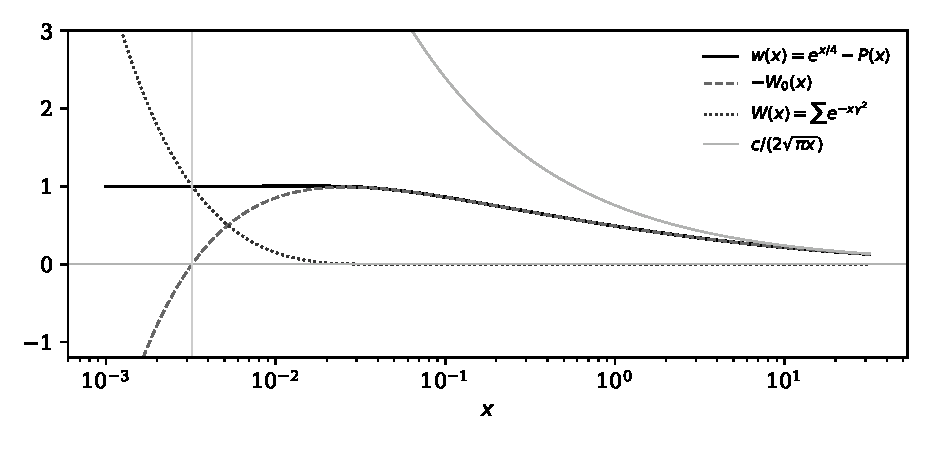
\includegraphics[width=0.9\textwidth]{rzfig/fig_w.pdf}
\caption{The function $w=W-W_0$ on a logarithmic scale, with its two components: the heat trace $W$ over the zeros and the negative smooth part $-W_0$. The vertical line is $x_*\approx0.00322$, where $W_0$ changes sign. To the left, $w$ differs from $e^{x/4}$ by less than $2\times10^{-13}$; to the right, $-W_0>0$, and from $x_1=0.004$ on it dominates any contribution of off line zeros to $W$. The faint curve is the asymptote $c/(2\sqrt{\pi x})$.}
\label{rz:fig:w}
\end{figure}

In arithmetic terms, Theorem~\ref{rz:thm:id} is the Gaussian smoothed Chebyshev bound
\[
\sum_{n\ge2}\frac{\Lambda(n)}{\sqrt n}\,e^{-(\log n)^2/4x}<\sqrt{4\pi x}\;e^{x/4}\qquad(x>0).
\]
The right side is $\int_0^\infty y^{-1/2}e^{-(\log y)^2/4x}\,dy$, the same smoothing applied to $dy$ in place of $d\psi(y)$, where $\psi(y)=\sum_{n\le y}\Lambda(n)$ is Chebyshev's function. The proof uses the zeros only through the ten below height $50$, the explicit bound for $N(T)$ and the monotone archimedean term $F$. To see what the primes alone give, write $\psi(y)=y+\Delta(y)$ and put $I(x)=\frac12e^{x/4}\operatorname{erfc}(\frac{\sqrt x}2)$.

\begin{proposition}\label{rz:prop:bias}
For $x>0$,
\[
w(x)=I(x)-Q_\Delta(x),\qquad Q_\Delta(x)=\frac{1}{\sqrt{4\pi x}}\int_{1^-}^\infty y^{-1/2}e^{-(\log y)^2/4x}\,d\Delta(y),
\]
with $I(x)\sim(\pi x)^{-1/2}$ and $w(x)\sim\frac c2(\pi x)^{-1/2}$ as $x\to\infty$. Hence $Q_\Delta(x)\sim-(\frac c2-1)(\pi x)^{-1/2}$ with $\frac c2-1\approx0.343$. On the other hand, any bound $|\Delta(y)|\le A\sqrt y\log^2y$ for $y\ge2$, including the one that RH implies, yields only $|Q_\Delta(x)|\le A\,(x/2+O(\sqrt x))$ after integration by parts.
\end{proposition}

\begin{proof}
With $d\Delta=d\psi-dy$, the main term is $(4\pi x)^{-1/2}\int_1^\infty y^{-1/2}e^{-(\log y)^2/4x}dy=(4\pi x)^{-1/2}\int_0^\infty e^{u/2-u^2/4x}du=\frac12e^{x/4}(1+\operatorname{erf}\frac{\sqrt x}2)$, and $e^{x/4}$ minus this is $I$. The asymptotics of $w$ are Theorem~\ref{rz:thm:w}. For the bound, integrate by parts and use $\frac{d}{dy}\{y^{-1/2}e^{-(\log y)^2/4x}\}=-y^{-3/2}e^{-(\log y)^2/4x}(\frac12+\frac{\log y}{2x})$ and $\int_0^\infty u^2e^{-u^2/4x}(\frac12+\frac u{2x})du=\frac{\sqrt\pi}2(2\sqrt x)^3\cdot\frac14+4x$; the boundary term at $1^-$ and the range $1\le y<2$ contribute $O(x^{-1/2})$.
\end{proof}

In this Gaussian weighting the error term $\Delta$ of the prime number theorem has a definite negative bias at large $x$, $Q_\Delta(x)\approx-0.343(\pi x)^{-1/2}$, which is $I+W_0$ up to an exponentially small term, and $w>0$ is the statement that $Q_\Delta(x)<I(x)$ for all $x$. Pointwise bounds on $\Delta$, which oscillates with both signs, cannot give this at large $x$: the margin that keeps $w$ positive there is of order $x^{-1/2}$, while a pointwise bound on $\Delta$ controls $Q_\Delta$ only up to order $x$; the function $D(y)=-A\sqrt y\log^2y$, in place of $\Delta$, gives $Q_D(x)=-A\bigl(x/2+2\sqrt{x/\pi}\bigr)$ by the computation in the proof, so the bound of Proposition~\ref{rz:prop:bias} cannot be improved using the size of $\Delta$ alone. Mean square information on $\Delta(y)/\sqrt y$ in the logarithmic scale, of the kind Cram\'er obtained under RH \cite{Cramer}, controls Gaussian smoothed quantities much better, and we make no claim that such information is insufficient. For $x\le0.004$ the primes alone suffice (Theorem~\ref{rz:thm:id}).

\subsubsection{The place of \texorpdfstring{$\varphi$}{phi} in the Bondesson hierarchy}\label{rz:sec:class}

Recall from Section~\ref{sec:ch3:hierarchy} the classes of laws on $[0,\infty)$ defined through the L\'evy density $k(x)/x$: the infinitely divisible laws (ID), the self decomposable laws (SD), for which $k$ is nonincreasing, the Bondesson class (BO), for which $k(x)/x$ is completely monotone, and the GGCs, for which $k$ is completely monotone. They are nested as $\mathrm{GGC}\subset\mathrm{SD}\subset\mathrm{ID}$ and $\mathrm{GGC}\subset\mathrm{BO}\subset\mathrm{ID}$ \cite{Bondesson,SvH}.

\begin{theorem}\label{rz:thm:class}
$\varphi\in\mathrm{ID}$ but $\varphi\notin\mathrm{SD}$, $\varphi\notin\mathrm{BO}$, and $\varphi$ is not a mixture of exponentials. In particular $\varphi$ is not a generalised gamma convolution.
\end{theorem}

\begin{proof}
ID is Theorem~\ref{rz:thm:id}.

SD. A law on $(0,\infty)$ with L\'evy density $k(x)/x$ is self decomposable if and only if $k$ is nonincreasing (Section~\ref{sec:ch3:hierarchy}). If $\varphi$ is not infinitely divisible there is nothing to prove, and if it is then $k=w$ by Theorem~\ref{rz:thm:w}. Now $w=e^{x/4}-P$, and $P$ together with every one of its derivatives vanishes at $0^+$, so $w'(0^+)=\frac14>0$ and $w$ strictly increases at the origin. No numerical value enters, and neither does Theorem~\ref{rz:thm:id}: the case split replaces it.

BO. Membership means that the L\'evy density $w(x)/x$ equals $\int e^{-tx}m(dt)$ for some $m\ge0$. Then $-\varphi'/\varphi(s)=\int_0^\infty xe^{-sx}\int e^{-tx}m(dt)\,dx=\int m(dt)/(s+t)^2$ is analytic on $\cut$, so $\varphi$ has no zeros or poles there and RH follows from Proposition~\ref{rz:prop:rh}. Under RH, Theorem~\ref{rz:thm:w} gives $w(x)=\int e^{-tx}dM(t)$, with $M(t)=N(\sqrt t)-\theta(\sqrt t)/\pi=1+S(\sqrt t)$ as in Theorem~\ref{rz:thm:thorin}, and since $M(0^+)=0$ an integration by parts gives $w(x)/x=\int e^{-tx}M(t)\,dt$. Uniqueness of Laplace transforms gives $M\,dt=m\ge0$, that is $S(\tau)\ge-1$ for almost all $\tau$. But by Selberg's central limit theorem \cite{Selberg46}, $S(\tau)<-1$ for a positive proportion of $\tau\in[T,2T]$ once $T$ is large, so $M<0$ on a set of positive measure. Numerically, for $527.71\le\tau\le527.90$, just below $\gamma_{289}=527.9036\ldots$, ball arithmetic gives $N(\tau)=288$ and $-1.143<S(\tau)<-1.008$, so $M<0$ there, and $S(\gamma_{289}^-)=-1.14548\ldots$ (\nolinkurl{verification_reciprocal_zeta/certify_k9_k2.py}).

Mixtures of exponentials. The law is a mixture of exponentials exactly when it has a completely monotone density, that is when $\varphi$ is a Stieltjes function, which requires $\Im\varphi(-t+i0)$ to have one sign. With $\zeta(\frac12+i\tau)=Z(\tau)e^{-i\theta(\tau)}$ we get $\Im\varphi(-\tau^2+i0)=\zeta(\frac12)\sin\theta(\tau)/\{(1+4\tau^2)Z(\tau)\}$. On $(0,\gamma_1)$, $Z$ has no zero while $\theta$ decreases through $-\pi$ at $\tau_\pi=3.43622\ldots$, so $\sin\theta$ changes sign.

GGC. Since GGC is contained in SD and in BO, either clause excludes it. The exclusion also follows directly, without computation. If $\varphi$ were the transform of a GGC then $-\varphi'/\varphi$ would be a Stieltjes function $a+\int U(dt)/(s+t)$ with $U\ge0$, that is $a+\int_0^\infty e^{-sx}\bigl(\int e^{-tx}U(dt)\bigr)dx$. Comparing with $-\varphi'/\varphi(s)=\int_0^\infty e^{-sx}w(x)\,dx$ of Theorem~\ref{rz:thm:w} on $s>\frac14$, uniqueness of Laplace transforms forces $a=0$ and $w(x)=\int e^{-tx}U(dt)$, completely monotone and in particular nonincreasing, against $w'(0^+)=\frac14>0$.
\end{proof}

The theorem is unconditional. Its ID clause rests on Theorem~\ref{rz:thm:id}, its BO clause on Selberg's central limit theorem for $S$, and its SD clause and the conclusion $\varphi\notin\mathrm{GGC}$ on no computation. Since mixtures of exponentials lie in BO \cite{Bondesson}, the mixture clause also follows from the BO clause, and from $f'(0^+)>0$ in Theorem~\ref{rz:thm:shape}; the direct argument, through the computed value of $\tau_\pi$, is an independent check.

The failures have two causes, and neither involves a zero off the line. Self decomposability and the GGC property fail because of the pole: the factor $1-4s$ that removes it puts $e^{x/4}$ into $w$, so the canonical function increases near the origin. This is a property of the normalisation, and Proposition~\ref{rz:prop:onlyhalf} shows the same on every line of the strip. The Bondesson property fails because the negative Thorin density of the gamma factor meets the fluctuations of the zeros about their smooth count, measured by $S$, which has large negative excursions: the first zero with $S(\gamma^-)<-1$ is $\gamma_{127}=282.4651$, where $S(\gamma_{127}^-)=-1.0063$, and the most negative value among the first $460$ zeros is at $\gamma_{289}$ (the seven such zeros are listed after Theorem~\ref{rz:thm:kappaexact}, and these values of $S$ are enclosed in ball arithmetic by the program cited in the proof). This failure would occur even if RH were true, and since $S$ is unbounded below, by Selberg and Tsang \cite{Selberg46,Tsang}, it recurs infinitely often. Both causes disappear for the completed function $R$, which is infinitely divisible and self decomposable with no hypothesis, by Theorem~\ref{thm:ch12:idsd} \cite[Theorem A]{P26}. What Theorem~\ref{rz:thm:id} adds there is the floor of Theorem~\ref{rz:thm:floor}: the canonical function of $e^{-c\sqs}R(s)$ splits into the arithmetic part $w$ and a completely monotone archimedean part (Section~\ref{ch:rz2}).

\subsubsection{The density of the law}

Let $X_\varphi$ be, as in Section~\ref{ch:rz2}, a random variable with $\E e^{-sX_\varphi}=\varphi(s)$. Differentiating the representation of Theorem~\ref{rz:thm:id} gives $-\varphi'(s)=\varphi(s)\int_0^\infty e^{-sx}w(x)\,dx$, which says that the measure $x\Pr(X_\varphi\in dx)$ is the convolution of the law of $X_\varphi$ with $w(x)\,dx$. Since $\varphi(s)\to0$ as $s\to\infty$, the law has no atom at $0$, so it is absolutely continuous, and its density $f$ satisfies Steutel's equation \cite[Proposition~III.4.16]{SvH}
\begin{equation}\label{rz:eq:steutel}
x\,f(x)=\int_0^xf(x-y)\,w(y)\,dy,\qquad x>0 .
\end{equation}
The right side is continuous in $x$ by dominated convergence, since $f$ is integrable and $w$ is bounded and continuous on $[0,\infty)$, so $f$ may be taken continuous on $(0,\infty)$. Near the origin, $w(y)=1+O(y)$ gives $f(x)=\bar f(x)(1+O(x))$ with $\bar f(x)=x^{-1}\int_0^xf$, and $\bar f(x)>0$ for every $x>0$, since otherwise $s\varphi(s)\to0$, whereas $s\varphi(s)\to-\zeta(\frac12)/4>0$. As $\bar f'=(f-\bar f)/x$, this gives $(\log\bar f)'=O(1)$ near $0$, so $\bar f$ and $f$ have a common positive limit $f(0^+)$, and dominated convergence in $s\varphi(s)=\int_0^\infty e^{-y}f(y/s)\,dy$, $f$ being bounded, gives $f(0^+)=\lim_{s\to\infty}s\varphi(s)=-\zeta(\frac12)/4\approx0.36509$.

At infinity the same equation gives $f(x)\sim w(x)/x\sim\frac{c}{2\sqrt\pi}x^{-3/2}\approx0.75773\,x^{-3/2}$, in three steps. First, $xf(x)\le\sup w$. Second, split the integral in \eqref{rz:eq:steutel}, written as $\int_0^xf(u)w(x-u)\,du$, at $u=x/2$: the part $u\le x/2$ is at most $\sup_{y\ge x/2}w(y)=O(x^{-1/2})$, and the part $u\ge x/2$ is at most $\sup_{[x/2,x]}f\cdot\int_0^{x/2}w=O(x^{-1})\,O(x^{1/2})$, so $f(x)=O(x^{-3/2})$. Third, with this bound the part $u\ge x/2$ is $O(x^{-1})=o(w(x))$, while the part $u\le x/2$ is $w(x)(1+o(1))$ by dominated convergence, since $w(x-u)/w(x)\to1$ for fixed $u$ and stays below $2$ for $u\le x/2$ and large $x$. Hence $xf(x)=w(x)(1+o(1))$. It follows that $\Pr(X_\varphi>x)\sim\frac{c}{\sqrt\pi}x^{-1/2}$ and $\E X_\varphi=\infty$, and since $\varphi(s)=1-c\sqs+O(s)$ gives $\varphi(s/n^2)^n\to e^{-c\sqs}$, the variable $X_\varphi$ lies in the domain of attraction of the positive stable law of index $\frac12$ that generates the building blocks \eqref{rz:eq:levy}. Figure~\ref{rz:fig:f} shows $f$ on logarithmic axes, recovered from $\varphi$ by numerical Laplace inversion; the value at $0^+$ and the $x^{-3/2}$ decay are its two straight portions.

\begin{figure}[htbp]
\centering
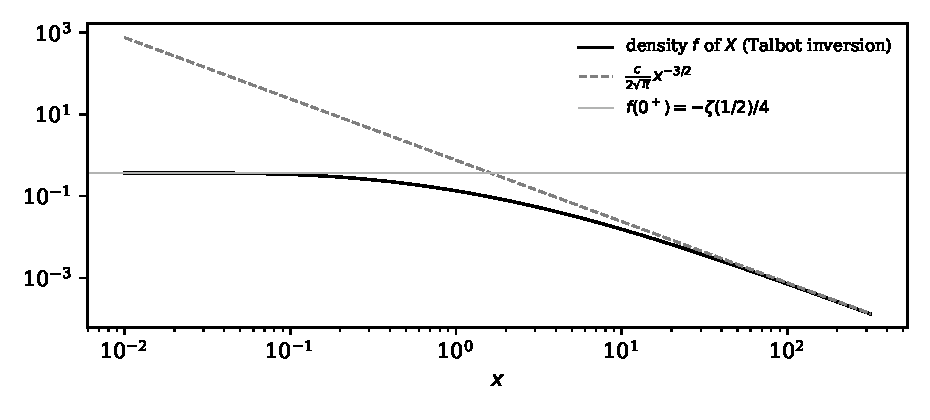
\includegraphics[width=0.9\textwidth]{rzfig/fig_f.pdf}
\caption{The density $f$ of the infinitely divisible law $X_\varphi$ with $\E e^{-sX_\varphi}=\varphi(s)$, computed by Talbot inversion, on logarithmic axes. It starts at $f(0^+)=-\zeta(\frac12)/4$ and decays like $\frac{c}{2\sqrt\pi}x^{-3/2}$. In the legend, $X$ is $X_\varphi$.}
\label{rz:fig:f}
\end{figure}

\begin{theorem}\label{rz:thm:shape}
$f(0^+)=-\zeta(\frac12)/4$ and $f'(0^+)=f(0^+)\,w'(0^+)=-\zeta(\frac12)/16\approx0.09127>0$. In particular $f$ is not monotone, so $X_\varphi$ is not a mixture of uniform laws on intervals $[0,a]$, and $f$ is not log convex and not completely monotone.
\end{theorem}

\begin{proof}
The value of $f(0^+)$ was found after \eqref{rz:eq:steutel}. Since $P$ and all its derivatives vanish at $0^+$, $w$ is continuously differentiable on $[0,\infty)$ with $w(0^+)=1$ and $w'(0^+)=\frac14$. Write \eqref{rz:eq:steutel} as $xf(x)=\int_0^xf(u)\,w(x-u)\,du$. Since $f$ is continuous on $(0,\infty)$ and bounded near $0$, the right side is differentiable, with derivative $f(x)w(0^+)+\int_0^xf(u)w'(x-u)\,du$, so $f$ is differentiable on $(0,\infty)$ and
\[
f'(x)=\frac1x\int_0^xf(u)\,w'(x-u)\,du\longrightarrow f(0^+)\,w'(0^+)\qquad(x\downarrow0),
\]
because $f$ and $w'$ are continuous at $0$. A nonincreasing density is required for a mixture of uniforms by Khintchine's theorem, and log convex or completely monotone densities are nonincreasing.
\end{proof}

\begin{proposition}\label{rz:thm:unimod}
$w'>0$ on $(0,0.004]$ and $w'<0$ on $[4.52,\infty)$. On $[0.004,4.6]$ a grid evaluation of $w'$ (computed, not proved) finds exactly one sign change, at $x_m=0.015851\ldots$, where $w(x_m)=1.003409\ldots$.
\end{proposition}

\begin{proof}
On $(0,0.004]$, $w'=\frac14e^{x/4}-P'(x)$ and $0\le P'(x)\le P'(0.004)<2\times10^{-9}$, since each prime term of $P'$ increases in $x$ there. For $x\ge0.004$ write $w'=W'-W_0'$. The zeros on the line contribute $-\sum\gamma^2e^{-x\gamma^2}<0$ to $W'$. Every zero below height $3\times10^{12}$ lies on the line \cite{PT21}, so an off line zero contributes at most $(\gamma^2+\frac14)e^{-x(\gamma^2-1/4)}$ with $\gamma>3\times10^{12}$. With $N(t+1)-N(t)\le2\log(t+1)$ from the proof of Theorem~\ref{rz:thm:id}, these contributions together are less than $e^{-10^{22}}\gamma_1^2e^{-x\gamma_1^2}$ for $x\ge0.004$, a negligible fraction of the term of $\gamma_1$; hence $W'<0$. By Proposition~\ref{rz:prop:bernstein}, with $\nu(dy)=2\sum_{k\ge0}e^{-(2k+\frac12)y}\,dy$ the measure defined there,
\begin{gather*}
-W_0'(x)=\frac{D(x)}{4\sqrt\pi\,x^{3/2}},\qquad D(x)=\theta'(0)+\frac12\int_0^\infty g\Bigl(\frac{y^2}{4x}\Bigr)\nu(dy),\\
g(u)=1-(1-2u)e^{-u}.
\end{gather*}
Since $g(0)=0$, $g'(0)=3$, $g$ is concave on $[0,\frac52]$ and $g\le1+2e^{-3/2}<3u$ beyond, $g(u)\le3u$ for all $u\ge0$. With $\int y^2\nu(dy)=4\sum_{k\ge0}(2k+\frac12)^{-3}<32.34$ this gives $D(x)\le\theta'(0)+12.13/x<0$ for $x\ge4.52$, and then both parts of $w'$ are negative.
\end{proof}

The computed statement comes from an evaluation of $w'$ on $[0.004,4.6]$ from the first 300 zeros and the integral for $W_0'$, on a grid of spacing $10^{-4}$ up to $0.05$ and $5\times10^{-3}$ beyond. On this grid $w'$ has exactly one sign change, at $0.01585$, and $|w'|\ge0.024$ at grid points more than $0.002$ from it; the prime and zero evaluations of $w'$ agree to $10^{-11}$ at $x=0.01$. Between two grid points $h$ apart at which $w'$ has one sign and $|w'|\ge0.024$, a further pair of sign changes would need $|w''|\ge2\cdot0.024/h$, that is $|w''|\ge9.6$ where the spacing is $5\times10^{-3}$ and $|w''|\ge480$ where it is $10^{-4}$. An upper bound on $|w''|$ below these values, which is not derived here, would exclude further sign changes away from $x_m$. Within $0.002$ of $x_m$ the grid gives no such margin, and a proof would also need $w''<0$ there, or a bound on $w'''$. Together these would turn the computation into a proof that $w$ is unimodal.

Numerically $f$ is unimodal as well: it rises from $0.365089$ to its maximum $0.366883$ at the mode $x=0.024046$ and then decreases to $0$ like $0.75773\,x^{-3/2}$, so its mode lies to the right of the maximum of $w$. Talbot and de Hoog inversion agree to twelve digits at every point used. Unimodality of $f$ remains open (Section~\ref{rz:sec:open}). Since $X_\varphi$ is infinitely divisible but not self decomposable, Yamazato's theorem that every self decomposable law is unimodal \cite{Yamazato78}, \cite[Theorem~53.1]{Sato99} does not apply, and the rise of $f$ near $0$ (Theorem~\ref{rz:thm:shape}) shows that the question is not trivial. Section~\ref{ch:sato} applies the theorem to the law of $X_R$, which is self decomposable, and to the shifted clocks $T_\alpha$ of Theorem~\ref{thm:poisson} with $\alpha\ge1$ (Corollary~\ref{sb:cor:unimodal}).

\subsubsection{Closure operations and the harmonic mean}

GGC is closed under independent sums and weak limits, and, by a theorem of Bondesson \cite{Bond2015}, under independent products. Any variable assembled from GGC variables by these operations is GGC, so Theorem~\ref{rz:thm:class} gives at once the following.

\begin{corollary}\label{rz:cor:hm}
$X_\varphi$ is not a sum or a product of independent GGC variables, nor a weak limit of such.
\end{corollary}

The reciprocal in $\varphi$ suggests a fourth operation, the harmonic mean. Closure under it would be the statement
\[
\mathrm{(H)}\qquad\text{if $V_1$ and $V_2$ are independent GGC variables, then so is $2V_1V_2/(V_1+V_2)$,}
\]
which would have widened Corollary~\ref{rz:cor:hm}; it is false.

\begin{proposition}\label{rz:prop:hmfalse}
(H) is false. If $E_1$ and $E_2$ are independent standard exponentials, then $H=2E_1E_2/(E_1+E_2)$ has density
\[
f_H(h)=e^{-h}\int_0^\infty\Bigl(1+\frac h{2u}\Bigr)e^{-u-h^2/4u}\,du,\qquad h>0,
\]
and $H$ is not a GGC.
\end{proposition}

\begin{proof}
For $h>0$, $2E_1E_2>h(E_1+E_2)$ holds if and only if $E_1,E_2>\frac h2$ and $(2E_1-h)(2E_2-h)>h^2$: both factors cannot be negative, since $E_1,E_2<\frac h2$ forces $|2E_1-h|,|2E_2-h|<h$. Substituting $E_1=\frac h2+u$, $E_2=\frac h2+v$ gives
\[
\Pr(H>h)=e^{-h}\iint_{uv>h^2/4}e^{-u-v}\,du\,dv=e^{-h}\int_0^\infty e^{-u-h^2/4u}\,du,
\]
so the survival function is $e^{-h}$ times a Laplace type integral. Differentiating under the integral, which is justified by the bound $\frac h{2u}e^{-u-h^2/4u}\le u^{-1/2}e^{-u}\sup_{y>0}ye^{-y^2}$, locally uniform in $h$, gives $f_H$. In terms of the modified Bessel functions of the second kind the two integrals are $h\,\mathrm{K}_1(h)$ and $h\{\mathrm{K}_0(h)+\mathrm{K}_1(h)\}$, by $\int_0^\infty u^{-\nu-1}e^{-u-h^2/4u}\,du=2(h/2)^{-\nu}\mathrm{K}_\nu(h)$ \cite[(10.32.10)]{DLMF}. Splitting the integral at $u=h$ shows that $f_H$ is bounded with $f_H(0^+)=1$.

Suppose $H$ were a GGC with drift $a$ and Thorin measure $U$ of total mass $\beta$. Since $f_H>0$ on $(0,\infty)$ and a GGC satisfies $H\ge a$ almost surely, $a=0$. Since $f_H$ is bounded, $s\,\E e^{-sH}=\int_0^\infty e^{-y}f_H(y/s)\,dy\to f_H(0^+)=1$, so $-\log\E e^{-sH}=\log s+o(1)$, while Fatou applied to $\int\log(1+s/t)\,U(dt)$ gives $\liminf_{s\to\infty}(-\log\E e^{-sH})/\log s\ge\beta$. Hence $\beta\le1$.

Now let $V$ be any GGC with zero drift and $\beta\le1$, and $\mathcal L(s)=\E e^{-sV}$. For $\Im s>0$ each $1+s/t$ lies in the upper half plane, so $\Im\log\mathcal L(s)=-\int\arg(1+s/t)\,U(dt)\in[-\pi\beta,0)\subseteq[-\pi,0)$, and $\mathcal L>0$ on $(0,\infty)$: $\mathcal L$ is a Stieltjes function \cite[Corollary~7.4]{boSSV}. In its representation $\mathcal L(s)=b_0+b_1/s+\int(s+r)^{-1}m(dr)$ \cite[Definition~2.1]{boSSV} we have $b_0=\lim_{s\to\infty}\mathcal L(s)=0$ and $b_1=0$, since $\mathcal L(0^+)=1$. So $\mathcal L(s)=\int_0^\infty e^{-sx}\bigl(\int e^{-rx}m(dr)\bigr)dx$ and the density of $V$ is $\int e^{-rx}m(dr)$, completely monotone and in particular nonincreasing.

But $f_H$ is not nonincreasing: $f_H(h)-1\sim h\log(1/h)$ as $h\downarrow0$, and $f_H$ attains $1.11125$ at $h=0.09765$ against $f_H(0^+)=1$. So $H$ is not a GGC.
\end{proof}

There is also a structural obstruction. The factorisation of $\varphi$ into $R$ and the gamma factor is a factorisation of Laplace transforms, that is a convolution of laws, while (H) acts on the variables themselves. The gamma factor is not a Laplace transform at all, since it tends to infinity with $s$, and \eqref{rz:eq:decon} shows that it enters only through deconvolution by stable laws. The one place where (H) could have acted is the positive part: $R$ is GGC if and only if RH holds, so an unconditional representation $X_R\overset{d}{=}2V_1V_2/(V_1+V_2)$ with $V_1,V_2$ independent GGC variables built from the primes and the gamma factor would have proved RH under (H). Proposition~\ref{rz:prop:hmfalse} removes the implication, and we know of no candidate representation. The kernel of the Vere-Jones identity is itself a harmonic mean of functions, $\sech(\lambda\sqs)=2/(e^{\lambda\sqs}+e^{-\lambda\sqs})$, of the stable transform $e^{-\lambda\sqs}$ and its reciprocal, which is not a transform; and each zero factor satisfies $1+u^2/\gamma^2=2/\{(1+iu/\gamma)^{-1}+(1-iu/\gamma)^{-1}\}$. Neither is a harmonic mean of independent variables, so neither brings (H) into play.

\subsection{The Vere-Jones weights and the L\'evy representation across the strip}\label{rz:sec:implications}

The weights $B_N$ of the logarithmic Vere-Jones representation (Theorem~\ref{rz:thm:saw}) are necklace polynomials evaluated at $p^{-1/2}$, and prime by prime the representation is a deformation of Euler's binary product. In its cyclotomic form the normalisation at the edge of the pole rests on the prime number theorem, and its heat trace form is a trace formula in which the zeros of $\zeta$ appear as a signed superposition of arithmetic progressions. The same weights, evaluated at $p^{-\sigma}$, carry the L\'evy representation to every vertical line of the critical strip, and on these lines the completed function $R_\sigma$ has the Thorin property exactly to the right of all zeros. Throughout this subsection $\sigma$ is the real part of the argument $z$ of $\zeta$.

\subsubsection{Necklace polynomials and the sign rule}

Let $M_k(q)=\frac1k\sum_{d\mid k}\mu(k/d)\,q^d$ be the necklace polynomial \cite{MR}, which for integer $q$ counts aperiodic necklaces of length $k$ in $q$ colours.

\begin{theorem}\label{rz:thm:necklace}
$B_N=0$ unless $N=p^n$ is a prime power, and then
\[
B_{p^n}=b_n\bigl(p^{-1/2}\bigr),\qquad b_n(q)=\sum_{i\ge0,\ 2^i\mid n}M_{n/2^i}(q).
\]
Equivalently, for $|y|<1$ and $0<q\le1$,
\begin{equation}\label{rz:eq:binarycyclo}
\frac1{1-qy}=\prod_{n\ge1}\bigl(1+y^n\bigr)^{b_n(q)},
\end{equation}
so that $\zeta(\frac12+u)=\prod_p\prod_n(1+p^{-nu})^{b_n(p^{-1/2})}$ for $\Re u>\frac12$. At $q=1$, $b_n(1)=1$ if $n$ is a power of $2$ and $0$ otherwise, and \eqref{rz:eq:binarycyclo} becomes Euler's binary identity $\frac1{1-y}=\prod_{j\ge0}(1+y^{2^j})$.
\end{theorem}

\begin{proof}
From the definition of $B_N$ in Theorem~\ref{rz:thm:saw}, $B_{p^n}=\sum_{jm=n}d_m\,a_{p^j}$ with $a_{p^j}=q^j/j$. Proposition~\ref{rz:prop:eta} gives $y^j=\sum_md_m\log(1+y^{mj})$; multiplying by $q^j/j$ and summing over $j$ gives $\sum_nb_n(q)\log(1+y^n)=\sum_jq^jy^j/j=-\log(1-qy)$, which is \eqref{rz:eq:binarycyclo}. The cyclotomic identity $\frac1{1-qy}=\prod_k(1-y^k)^{-M_k(q)}$ and $\log(1+y^n)=\log(1-y^{2n})-\log(1-y^n)$ give, comparing coefficients of $\log(1-y^n)$, the recursion $b_n=M_n+b_{n/2}$ for even $n$ and $b_n=M_n$ for odd $n$, whose solution is the stated sum. At $q=1$, $M_k(1)=\frac1k\sum_{d\mid k}\mu(k/d)=\delta_{k,1}$.
\end{proof}

The identity \eqref{rz:eq:binarycyclo} is a $2$ adic variant of the cyclotomic identity of Metropolis and Rota \cite{MR}; we have not found it stated in this form, but it may well be known in the combinatorics of necklaces. Its exponents include $b_2=\frac{q^2+q}2$, $b_3=\frac{q^3-q}3$, $b_4=\frac{q^4}4+\frac{q^2}4+\frac q2$, $b_6=\frac{q^6+q^3-q^2-q}6$, which give $B_4$, $B_8$ and $B_9$ of Theorem~\ref{rz:thm:saw} and, at $p=2$, $B_{16}$ and $B_{64}$, and numerically both sides agree to $25$ digits at $q=2^{-1/2}$, $y=\frac12$. The identity factors a geometric series into products of $1+y^n$, and applied prime by prime it factors the zeta function into solved models. So the Vere-Jones factorisation of each Euler factor is a deformation of Euler's binary product: on the line $\sigma=0$, where $q=p^{-\sigma}=1$, every exponent is $0$ or $1$ and every factor $1+p^{-2^ju}$ is a solved model with unit multiplicity, while on the critical line the exponents become necklace polynomials evaluated at $p^{-1/2}$.

\begin{proposition}\label{rz:prop:signs}
For every prime $p$, with $q=p^{-1/2}$: $b_{2^a}(q)>0$ for all $a\ge1$, and for odd $n>1$, $b_n(q)\ne0$ and the sign of $b_n(q)$ is $(-1)^{\omega(n)}$, where $\omega(n)$ is the number of distinct prime factors of $n$.
\end{proposition}

\begin{proof}
For $n=2^a$, $b_n=q+\sum_{j=1}^a\frac{q^{2^j}-q^{2^{j-1}}}{2^j}=\frac q2+\frac{q^2}4+\cdots+\frac{q^{2^{a-1}}}{2^a}+\frac{q^{2^a}}{2^a}>0$. For odd $n$, $b_n=M_n$. Put $\ell=\operatorname{rad}(n)$ and $\tilde q=q^{n/\ell}\le q\le2^{-1/2}$; then $nM_n(q)=\sum_{k\mid\ell}\mu(\ell/k)\tilde q^k=(-1)^{\omega(n)}\bigl(\tilde q+\sum_{k\mid\ell,k>1}\pm\tilde q^k\bigr)$, and the divisors $k>1$ of the odd squarefree $\ell$ are distinct odd integers at least $3$, so $\sum_{k>1}\tilde q^k<\sum_{m\ \mathrm{odd}\ge3}\tilde q^m=\tilde q\cdot\frac{\tilde q^2}{1-\tilde q^2}\le\tilde q$.
\end{proof}

For odd $n$ the weights are negative exactly when $n$ has an odd number of distinct prime factors, beginning with $n=3,5,7,9,11,13$; for even $n$ other than powers of $2$ the sign depends on how the $2$ adic parts combine (for $p=2$, $b_6,b_{10},b_{12},b_{14}<0$ while $b_{30},b_{42}>0$). Among $2\le n\le60$ there are $42$ negative exponents for each of $p=2,3,5,7$. Section~\ref{rz:sec:polya} returns to what these fractional and negative multiplicities mean for the zeros.

The weights $B_N$ and $d_m$ also govern the truncation of the sawtooth expansion of $S$. The sawtooth $\Sigma_\lambda$ of Lemma~\ref{rz:lem:saw} has the Fourier series $\Sigma_\lambda(\tau)=\sum_{j\ge1}(-1)^j\frac{\sin(j\lambda\tau)}{\pi j}$, so the formal series $\sum_NB_N\Sigma_{\log N}(\tau)$ is a double series in $(N,j)$ whose frequencies are $j\log N$.

\begin{proposition}\label{rz:prop:sawtrunc}
Truncate the double series by frequency, keeping the terms with $j\log N\le L$. Then
\[
\sum_{\substack{N,j\\ j\log N\le L}}B_N\,(-1)^j\frac{\sin(j\tau\log N)}{\pi j}=-\frac1\pi\sum_{n\le e^L}\frac{\Lambda(n)}{\sqrt n\log n}\sin(\tau\log n),
\]
the classical truncated series for $S(\tau)$. Truncation by $N\le N_0$ instead is not equivalent: it keeps the harmonics $j\log N>\log N_0$ of each retained sawtooth without the terms of larger $N$ that cancel them.
\end{proposition}

\begin{proof}
With $N=n^m$, the frequency is $r\log n$ with $r=mj$, and the constraint $j\log N\le L$ is $r\log n\le L$, which does not separate $m$ from $j$. The coefficient of $\sin(r\tau\log n)$ is $-\frac{a_n}\pi\sum_{mj=r}d_m\frac{(-1)^{j+1}}j$, and $\sum_{mj=r}d_m(-1)^{j+1}j^{-1}$ has Dirichlet series $\eta(1+v)^{-1}\eta(1+v)=1$, so it is $\delta_{r,1}$.
\end{proof}

So the sawtooth expansion contains nothing that the classical series lacks once it is truncated consistently, and truncating it by the index $N$ is worse. Numerically, on a uniform grid of step $10^{-3}$ in $\tau\in[10,50]$ and with the Ces\`aro weight $1-\log N/\log N_0$, the root mean square error against $S(\tau)$ is $0.228$, $0.223$, $0.218$ for $N_0=10^3,10^4,10^5$, against $0.146$, $0.128$, $0.115$ for the classical series with the same weight, the root mean square of $S$ itself being $0.320$; the script \texttt{sawtooth\_truncation.py} computes these values, and the step $5\times10^{-4}$ changes none of their digits. The bound $|\Sigma_\lambda|\le\frac12$ does not help either, since $\frac12\sum_{N\le N_0}|B_N|$ is $9.0$, $18.5$, $40.6$ at the same $N_0$ and grows like $\sqrt{N_0}/\log N_0$.

\subsubsection{The cyclotomic form, the prime number theorem and a trace formula}

The cyclotomic identity gives a second factorisation, into the blocks $1-N^{-u}$:
\[
\frac1{\zeta(\frac12+u)}=\prod_p\prod_{k\ge1}\bigl(1-p^{-ku}\bigr)^{M_k(p^{-1/2})},\qquad\Re u>\tfrac12 .
\]
Each block $1-e^{-\lambda u}=2e^{-\lambda u/2}\sinh(\lambda u/2)$ is again a solved model, now with a sinh lattice: with $u=\sqs$, $\frac{\sinh(\lambda\sqs/2)}{\lambda\sqs/2}=\prod_{m\ge1}\bigl(1+\frac{s}{(2\pi m/\lambda)^2}\bigr)$, a reciprocal GGC with unit atoms at $(2\pi m/\lambda)^2$. The sinh blocks are the local zeta factors on the line $\sigma=0$, and unlike the sech blocks they vanish at $u=0$. Normalising the product at $u\to0$ therefore requires two identities.

\begin{proposition}\label{rz:prop:pnt}
For $0<q<1$, summing over $k$ in increasing order,
\[
\sum_{k\ge1}M_k(q)=0,\qquad\sum_{k\ge1}M_k(q)\log k=\log(1-q).
\]
Both follow from the prime number theorem in the forms $\sum_m\mu(m)/m=0$ and $\sum_m\mu(m)\log m/m=-1$.
\end{proposition}

\begin{proof}
$\sum_{k\le K}M_k(q)=\sum_d\frac{q^d}d\sum_{m\le K/d}\frac{\mu(m)}m$. The inner sums are bounded by $1$ in absolute value and tend to $0$, so dominated convergence gives $0$. Similarly $\sum_{k\le K}M_k(q)\log k=\sum_d\frac{q^d}d\sum_{m\le K/d}\frac{\mu(m)\log(dm)}m\to\sum_d\frac{q^d}d(-1)=\log(1-q)$, using $\sum\mu(m)/m=0$ for the $\log d$ part.
\end{proof}

The two identities are the per prime analogues of these forms of the prime number theorem, and heuristically they are what makes the cyclotomic product of solved models converge at the edge $u\to0$: $\prod_k(1-y^k)^{-M_k(q)}$ behaves near $y=1$ like $(1-y)^{-\sum M_k}\prod_kk^{-M_k}$, and the finite limit $\frac1{1-q}$ requires both. The sech form of Theorem~\ref{rz:thm:necklace} carries the same information in the value $1/\eta(1)=1/\log2$ at $v=0$ of the continuation of $\sum_md_mm^{-v}=1/\eta(1+v)=1/((1-2^{-v})\zeta(1+v))$; the series $\sum_md_m$ itself diverges, since $d_{2^k}=\frac12$ for every $k\ge1$ (Proposition~\ref{rz:prop:eta}).

In heat trace form the Vere-Jones representation becomes a trace formula. Proposition~\ref{rz:prop:theta} and Poisson summation give, for every $x>0$,
\begin{equation}\label{rz:eq:pseudotrace}
\sum_{\gamma>0}e^{-x\gamma^2}-W_0(x)=e^{x/4}+\sum_{p}\sum_{n\ge1}b_n(p^{-1/2})\Bigl[\sum_{k\ge0}e^{-x\left(\frac{(2k+1)\pi}{n\log p}\right)^2}-\frac{n\log p}{4\sqrt{\pi x}}\Bigr],
\end{equation}
where the left side is written under RH and is $W(x)-W_0(x)$ in general, and the double series converges absolutely once each bracket is written in its theta form. The left side is the heat trace of the zeros net of its smooth part; the right side is the pole plus the heat traces of the arithmetic progressions $\frac{(2k+1)\pi}{n\log p}$, the pseudo zeros of the blocks, each net of its own mean. So in heat trace the zeros of $\zeta$ are a signed superposition of arithmetic progressions with spacings $2\pi/(n\log p)$, the progression of $p^n$ entering with the necklace weight $b_n(p^{-1/2})$. Heuristically, constructive interference of the progressions places the mass at the ordinates $\gamma$, and the negative weights of Proposition~\ref{rz:prop:signs} remove the mass from the other points of the progressions.

The trace formula does not give positivity of the Thorin measure of $R$. The obstruction is explicit: the weights $b_n(p^{-1/2})$ are not nonnegative integers, for odd $n$ their signs follow the parity of $\omega(n)$, and the passage from the binary product at $q=1$, where every multiplicity is $0$ or $1$, to the critical line at $q=p^{-1/2}$ is a deformation of the exponents in which integrality and positivity are lost together. A proof of RH along these lines would have to show that the interference of the progressions in \eqref{rz:eq:pseudotrace}, with exactly these weights, produces a positive measure; Section~\ref{rz:sec:open} poses the deformation from $q=1$ to $q=p^{-1/2}$ as a problem.

\subsubsection{The L\'evy and Thorin representations across the strip}\label{rz:sec:levystrip}

For $\sigma>1$ the Vere-Jones representation is a statement about the classical zeta distribution (Section~\ref{rz:sec:strip}): $\zeta(\sigma+i\tau)/\zeta(\sigma)=\E e^{-i\tau\log N_\sigma}$ where $\Pr(N_\sigma=n)=n^{-\sigma}/\zeta(\sigma)$, and $\log N_\sigma$ is compound Poisson with L\'evy measure $\nu_\sigma=\sum_n\frac{\Lambda(n)}{n^\sigma\log n}\delta_{\log n}$. Theorem~\ref{rz:thm:necklace} decomposes this L\'evy measure as
\[
\nu_\sigma=\sum_p\sum_{n\ge1}b_n(p^{-\sigma})\,\nu^{\mathrm{alt}}_{n\log p},\qquad\nu^{\mathrm{alt}}_\lambda=\sum_{k\ge1}\frac{(-1)^{k+1}}k\,\delta_{k\lambda},
\]
where $\nu^{\mathrm{alt}}_\lambda$ is the formal L\'evy measure of the fair coin $\lambda B$, $B\in\{0,1\}$, whose characteristic function $\frac12(1+e^{-i\lambda\tau})$ is the sech block. At $\sigma=0$ the weights $b_n(1)$ are $1$ at the powers of $2$ and $0$ otherwise, and the decomposition says, formally (there is no uniform law on the integers), that a uniformly random integer has independent fair binary digits in each prime exponent. For $\sigma>1$ there is also a positive decomposition: by $\frac1{1-qy}=\prod_j(1+q^{2^j}y^{2^j})$, the exponent of $p$ in $N_\sigma$ has independent binary digits with $\Pr(\text{digit }j=1)=\frac{p^{-2^j\sigma}}{1+p^{-2^j\sigma}}$. The Vere-Jones form keeps the coins fair and moves $p^{-\sigma}$ into the multiplicities; the binary digit form keeps unit multiplicities and biases the coins.

Inside the critical strip neither form survives as a characteristic function, since $|\zeta(\sigma+i\tau)|$ is unbounded in $\tau$ for $0<\sigma<1$ and the Dirichlet series diverges (Section~\ref{rz:sec:strip}); the heat kernel supplies the replacement. For $0<\sigma<1$ put
\[
\varphi_\sigma(s)=\frac{\zeta(\sigma)}{(1-s/(1-\sigma)^2)\,\zeta(\sigma+\sqs)},\qquad\varphi_{1/2}=\varphi .
\]

\begin{theorem}\label{rz:thm:levystrip}
For $0<\sigma<1$ and $s>(1-\sigma)^2$, $-\varphi_\sigma'/\varphi_\sigma(s)=\int_0^\infty e^{-sx}w_\sigma(x)\,dx$, where $w_\sigma$ has the three equivalent forms
\begin{align*}
w_\sigma(x)&=e^{(1-\sigma)^2x}-\frac{1}{\sqrt{4\pi x}}\sum_{n\ge2}\frac{\Lambda(n)}{n^\sigma}e^{-(\log n)^2/4x}\\
&=e^{(1-\sigma)^2x}+\sum_p\sum_{n\ge1}b_n(p^{-\sigma})\,h_{n\log p}(x)\\
&=\tfrac12e^{(1-\sigma)^2x}\operatorname{erfc}\bigl((1-\sigma)\sqrt x\bigr)+\sum_{\gamma>0}\Re\Bigl[e^{a_\gamma^2x}\operatorname{erfc}(a_\gamma\sqrt x)\Bigr]\\
&\qquad+\frac{\gamma_E+\log\pi}{4\sqrt{\pi x}}+\sum_{k\ge0}\Bigl[\tfrac12e^{a_k^2x}\operatorname{erfc}(a_k\sqrt x)-\frac1{4(k+1)\sqrt{\pi x}}\Bigr],
\end{align*}
with $h_\lambda$ the Jacobi theta function of Proposition~\ref{rz:prop:theta}, $a_\gamma=\sigma-\frac12-i\gamma$ (the last form written under RH; in general $\gamma$ runs over $-i(\rho-\frac12)$), and $a_k=2k+2+\sigma$. As $x\to\infty$, $w_\sigma(x)\sim\frac{\zeta'(\sigma)/\zeta(\sigma)}{2\sqrt{\pi x}}$, with $\zeta'(\sigma)/\zeta(\sigma)>0$ on $(0,1)$. If $w_\sigma\ge0$, then $\varphi_\sigma$ is the Laplace transform of an infinitely divisible law on $(0,\infty)$ with L\'evy density $w_\sigma(x)/x$:
\[
\log\varphi_\sigma(s)=-\int_0^\infty\bigl(1-e^{-sx}\bigr)\frac{w_\sigma(x)}x\,dx,\qquad\Re s>0 .
\]
\end{theorem}

\begin{proof}
The first form is the argument of Theorem~\ref{rz:thm:w} with the pole now at $s=(1-\sigma)^2$. For the second, regroup $\sum_nb_n(q)\,n\log p\sum_j(-1)^je^{-(jn\log p)^2/4x}$ by $r=jn$: with $nb_n=\sum_{ab=n}a\,d_aq^b$ the coefficient of $e^{-(r\log p)^2/4x}$ is $\sum_{b\mid r}q^b\sum_{ja=r/b}a\,d_a(-1)^j=-q^r$, since the inner sum is $-\delta_{r/b,1}$ (Proposition~\ref{rz:prop:theta}); this is the prime $p$ part of the first form. For the third, insert the Hadamard product of $\zeta'/\zeta$ into $-\varphi_\sigma'/\varphi_\sigma=\frac1{s-(1-\sigma)^2}+\frac1{2\sqs}\frac{\zeta'}\zeta(\sigma+\sqs)$; the pole terms combine to $\frac1{2\sqs(\sqs+1-\sigma)}$, and each $\frac1{\sqs(\sqs+a)}$ is the transform of $e^{a^2x}\operatorname{erfc}(a\sqrt x)$. At $\sigma=\frac12$ this reduces to $w=W-W_0$ with Proposition~\ref{rz:prop:W0erfc}.

The asymptotic follows from the third form term by term. Uniformly for $|\arg a|\le\frac{3\pi}4-\epsilon$ and $|a|\sqrt x\ge1$,
\[
\tfrac12e^{a^2x}\operatorname{erfc}(a\sqrt x)=\frac1{2a\sqrt{\pi x}}+O\bigl(|a|^{-3}x^{-3/2}\bigr);
\]
every $a$ in the third form has $|\arg a|<\frac\pi2+\frac1{14}$, and $\sum|a|^{-3}$ converges. So $w_\sigma(x)=C_\sigma/(2\sqrt{\pi x})+O(x^{-3/2})$ with
\[
C_\sigma=\frac1{1-\sigma}+\sum_\rho\frac1{\sigma-\rho}+\frac{\gamma_E+\log\pi}2+\sum_{k\ge0}\Bigl(\frac1{2k+2+\sigma}-\frac1{2k+2}\Bigr),
\]
the sum over $\rho$ taken in conjugate pairs, and $C_\sigma=\zeta'(\sigma)/\zeta(\sigma)$ by the Hadamard product of $\xi$. Infinite divisibility follows from $w_\sigma\ge0$ by Landau's theorem as in Theorem~\ref{rz:thm:id}, since $\varphi_\sigma$ is analytic near $(0,\infty)$: $\zeta(\sigma+x)\ne0$ for $x>0$ and the pole at $x=1-\sigma$ is cancelled.
\end{proof}

Numerically $w_\sigma$ is positive on every line we tried. We evaluated it on $300$ points of $x\in[10^{-4},10^3]$, from the prime form for $x\le0.02$ and the zero form beyond, for $\sigma=0.05,0.1,0.25,0.4,0.5,0.6,0.75,0.9,0.99$; the two forms agree to $5\times10^{-6}$ at $x=0.01$ and $0.05$. In every case the minimum is attained at the largest $x$, and $2\sqrt{\pi x}\,w_\sigma(x)$ at $x=10^3$ equals $1.872$, $1.913$, $2.087$, $2.377$, $2.682$, $3.154$, $4.596$, $10.16$, $41.1$, against $\zeta'(\sigma)/\zeta(\sigma)$, which is $1.873$, $1.914$, $2.088$, $2.379$, $2.686$, $3.162$, $4.628$, $10.60$, $100.58$ at the same nine values of $\sigma$. The agreement is close up to $\sigma=0.75$ and breaks down as $\sigma\to1$, where the pole makes the approach slow and the asymptotic has not been reached at $x=10^3$. So $w_\sigma>0$ is checked only for $x\le10^3$ and at nine values of $\sigma$. Whether the L\'evy density is positive on every vertical line of the strip is open (Problem~\ref{rz:prob:strip}).

For the Thorin representation two families have to be distinguished: $\varphi_\sigma$, which carries the gamma factor and the pole, and the completed function $R_\sigma(s)=\xi(\sigma)/\xi(\sigma+\sqs)$. For $\sigma>\frac12$ the second is, with no hypothesis, the Laplace transform of an infinitely divisible law obtained by tilting and subordinating the law of $X_R$ (Theorem~\ref{bp:thm:alpha} of Section~\ref{ch:bphit} and the proof of Proposition~\ref{sm:prop:cf} of Section~\ref{ch:strip}, where $R_\sigma$ is written $\varphi_\alpha$). The first never has the Thorin property, and the proof uses no computation and nothing about $\zeta$ beyond Theorem~\ref{rz:thm:levystrip}.

\begin{proposition}\label{rz:prop:onlyhalf}
For every $\sigma\in(0,1)$, $\varphi_\sigma$ is not the Laplace transform of a GGC, and if it is infinitely divisible it is not self decomposable.
\end{proposition}

\begin{proof}
The argument is that of Theorem~\ref{rz:thm:class}. By Theorem~\ref{rz:thm:levystrip}, $-\varphi_\sigma'/\varphi_\sigma(s)=\int_0^\infty e^{-sx}w_\sigma(x)\,dx$ for $s>(1-\sigma)^2$, with
\[
w_\sigma=e^{(1-\sigma)^2x}-P_\sigma,\qquad P_\sigma(x)=\frac1{\sqrt{4\pi x}}\sum_{n\ge2}\frac{\Lambda(n)}{n^\sigma}e^{-(\log n)^2/4x}.
\]
Every derivative of $P_\sigma$ vanishes at $0^+$, so $w_\sigma(x)=1+(1-\sigma)^2x+o(x)$ and $w_\sigma$ strictly increases near the origin. If $\varphi_\sigma$ were a GGC transform, then $-\varphi_\sigma'/\varphi_\sigma=a+\int U(dt)/(s+t)$ with $a\ge0$ and $U\ge0$ satisfying the Thorin integrability conditions, so that $k_U(x)=\int e^{-tx}U(dt)$ is integrable near $0$ and, by Tonelli, $\int U(dt)/(s+t)=\int_0^\infty e^{-sx}k_U(x)\,dx$ for $s>(1-\sigma)^2$. Letting $s\to\infty$ gives $a=0$, and uniqueness of the Laplace transform gives $w_\sigma=k_U$, which is completely monotone and so nonincreasing, a contradiction. If $\varphi_\sigma$ is infinitely divisible, the same uniqueness identifies its L\'evy density as $w_\sigma(x)/x$, and self decomposability would require $w_\sigma$ to be nonincreasing.
\end{proof}

As on the critical line, the obstruction is the factor $1-s/(1-\sigma)^2$ that removes the pole, and it says nothing about the zeros. Beyond it, for $\frac12<\sigma<1$ with $\sup_\rho\Re\rho<\sigma$, the Thorin density $\frac{1}{2\pi\sqrt t}\Re\frac{\zeta'}{\zeta}(\sigma+i\sqrt t)$ given by Lemma~\ref{rz:lem:inv} also takes negative values on every line we examined (the minimum of $\Re\frac{\zeta'}{\zeta}(\sigma+i\tau)$ over $\tau\in(0,60]$ is $-1.049$, $-0.995$, $-0.867$, $-0.769$, $-0.721$ at $\sigma=0.55,0.6,0.75,0.9,0.99$), but the proposition does not need this.

The completed functions $R_\sigma$ carry the zeros. Theorem~\ref{rz:thm:threshold} is Theorem~\ref{thm:poisson} of Section~\ref{ch:clock} in the variable of this chapter.

\begin{theorem}\label{rz:thm:threshold}
Let $\sigma\ge\frac12$. Then $R_\sigma(s)=\xi(\sigma)/\xi(\sigma+\sqs)$ is the Laplace transform of a GGC if and only if $\zeta$ has no zero $\rho$ with $\Re\rho>\sigma$. In that case its Thorin measure is the Poisson smoothed zero density
\[
U_\sigma(dt)=\frac{1}{2\pi\sqrt t}\sum_\rho\frac{\sigma-\beta_\rho}{(\sigma-\beta_\rho)^2+(\sqrt t-\gamma_\rho)^2}\,dt,
\]
the sum running over all nontrivial zeros $\rho=\beta_\rho+i\gamma_\rho$, counted with multiplicity, of both signs of $\gamma_\rho$, and taken symmetrically; each zero on $\Re\rho=\sigma$ with $\gamma_\rho>0$ contributes a unit atom at $\gamma_\rho^2$ instead of its kernel. Consequently $R_\sigma$ is a GGC for every $\sigma\ge1$, unconditionally, and
\[
\Theta:=\sup_\rho\Re\rho=\inf\{\sigma\ge\tfrac12:\ R_\sigma\text{ is a GGC}\}.
\]
RH is the statement $\Theta=\frac12$, that is, that $R_{1/2}=R$ is a GGC.
\end{theorem}

\begin{proof}
A zero with $\Re\rho>\sigma$ gives $\sqs=\rho-\sigma$ on the principal branch and hence a pole of $R_\sigma$ in $\cut$, so $R_\sigma$ is not a GGC. Suppose there is none. Write the zeros with positive ordinate, counted with multiplicity, as $\rho=\beta+i\gamma$, put $a=\sigma-\beta\ge0$, and let $\mathcal P_a(x)=a/\{\pi(a^2+x^2)\}$, for $a>0$, be the Cauchy density of scale $a$ (the Poisson kernel $P_a$ of Section~\ref{ch:clock}). Hadamard's product \cite[Chapter~12]{Davenport}, with each $\rho$ paired with $\bar\rho$, gives $\xi(z)=\xi(0)\prod_{\gamma>0}(1-z/\rho)(1-z/\bar\rho)$, absolutely convergent since $\sum_\rho|\rho|^{-2}<\infty$, and hence for $s>0$ and $q=\sqs$
\[
R_\sigma(s)=\prod_{\gamma>0}\frac{a^2+\gamma^2}{(q+a)^2+\gamma^2}.
\]
For $a>0$ let $U_{a,\gamma}(dt)=\{\mathcal P_a(\sqrt t-\gamma)+\mathcal P_a(\sqrt t+\gamma)\}\,dt/(2\sqrt t)$, and let $U_{0,\gamma}=\delta_{\gamma^2}$. The substitution $t=\tau^2$, the identity $1/(s+\tau^2)=(\pi/q)\mathcal P_q(\tau)$ and $\mathcal P_a*\mathcal P_q=\mathcal P_{a+q}$ give
\[
\int_0^\infty\frac{U_{a,\gamma}(dt)}{s+t}=\frac{q+a}{q\{(q+a)^2+\gamma^2\}}=\frac{d}{ds}\log\{(q+a)^2+\gamma^2\},
\]
which also holds for $a=0$. Integrating over $(0,s]$ with Tonelli, $\int\log(1+s/t)\,U_{a,\gamma}(dt)=\log\{((q+a)^2+\gamma^2)/(a^2+\gamma^2)\}$, which is nonnegative and at most $(s+2\sigma\sqs)/\gamma^2$. Since $\sum_{\gamma>0}\gamma^{-2}<\infty$, Tonelli's theorem shows that $U_\sigma=\sum_{\gamma>0}U_{a,\gamma}$ is a positive measure with $\int\log(1+s/t)\,U_\sigma(dt)=-\log R_\sigma(s)<\infty$, which gives the Thorin integrability conditions, and that $R_\sigma(s)=\exp\{-\int\log(1+s/t)\,U_\sigma(dt)\}$ for $s>0$. So $R_\sigma$ is the Laplace transform of a GGC with Thorin measure $U_\sigma$, whose density is the stated sum, grouped by the pairs $\rho,\bar\rho$, and each zero on $\Re\rho=\sigma$ with $\gamma_\rho>0$ gives the atom $\delta_{\gamma_\rho^2}$. For $\sigma\ge1$ the hypothesis holds by the Euler product.

For $\sigma>\Theta$ the density also follows from Lemma~\ref{rz:lem:inv}: then $-R_\sigma'/R_\sigma(s)=\frac1{2\sqs}\frac{\xi'}\xi(\sigma+\sqs)$ is $O(|s|^{-1/2})$ near $0$, $O(|s|^{-1/2}\log|s|)$ at infinity uniformly on $\cut$ (by the partial fraction formula for $\zeta'/\zeta$ \cite[Chapter~15]{Davenport}, since every zero lies at distance at least $\sigma-\Theta$ from the half plane $\Re z\ge\sigma$), and continuous up to the cut away from $0$, and at $\sqs=i\tau$ the lemma gives the density $\frac1{2\pi\tau}\Re\frac{\xi'}\xi(\sigma+i\tau)=\frac1{2\pi\tau}\sum_\rho\Re\frac1{\sigma+i\tau-\rho}$, summed symmetrically.
\end{proof}

Moving the line to the right of all zeros replaces the atoms $\delta_{\gamma^2}$ by Poisson kernels of width $\sigma-\beta_\rho$ in $\sqrt t$, and the GGC property then holds. The kernels of the zeros with $\gamma_\rho<0$ are centred at negative values of $\sqrt t$ and are positive on $t>0$; they disappear only in the limit $\sigma\downarrow\beta_\rho$. RH says that the Poisson kernels can be sharpened all the way to atoms at $\sigma=\frac12$ without any of them acquiring a negative width. The quasi Riemann Hypothesis $\Theta<1$, announced in October 2026 with $\Theta\le\frac78$ (Section~\ref{sec:ch25:open}), is the statement that $R_\sigma$ is a GGC for some $\sigma<1$; it is step~7 of the path to RH in Section~\ref{ch:path} (Table~\ref{tab:ch25:path}), and short of it Section~\ref{ch:almost} shows with no hypothesis that for $\frac12<\sigma<1$, in the density $\rho_{\sigma-1/2}$ of \eqref{eq:rho}, the Cauchy kernels of the zeros to the right of $\sigma$, if there are any, carry below height $T$ a vanishing fraction of the mass of the kernels of the other zeros as $T\to\infty$. Numerically $\min_{0<\tau\le70}\Re\frac{\xi'}\xi(\sigma+i\tau)$ is $4.6\times10^{-5}$, $0.0046$, $0.0116$, $0.0231$ at $\sigma=0.501,0.6,0.75,1$, attained as $\tau\to0$.

\subsection{P\'olya and Cardon theory for the solved models}\label{rz:sec:polya}

P\'olya's theory of Fourier transforms with only real zeros, and its extension by Cardon, is built from the objects that the Vere-Jones step produces: cosines, hyperbolic cosines and their products. The solved models are special cases of that theory; $\zeta$ is not, because its multiplicities are neither integers nor nonnegative; and the theory suggests a construction, the Cardon route, whose difficulty at the boundary of a strip points to the lattice of Biane, Pitman and Yor. Throughout, $\Phi$ is the P\'olya kernel and $\Xi(\tau)=\int\Phi(t)\cos(\tau t)\,dt$, as in \eqref{eq:ch2:Phi} with the variable written $t$; $\Phi$ is even, analytic in the strip $|\Im t|<\pi/4$, and has a natural boundary on the lines $\Im t=\pm\pi/4$ \cite[Chapter~11, Section~1.4, and Chapter~5, Section~3.2]{Remmert98}. The P\'olya variable $X$ of Section~\ref{ch:clock} has density $\Phi/\Xi(0)$ and moment generating function $\E e^{hX}=\xi(\frac12+h)/\xi(\frac12)$, by \eqref{eq:ch2:mgf}. In this subsection $G$ denotes a function of the Laguerre P\'olya class, not the gamma factor.

\subsubsection{Solved models and the Laguerre P\'olya class}

On the critical line the block $1+N^{-\sqs}$ becomes
\[
1+N^{-i\tau}=2e^{-i\tau\ell/2}\cos\bigl(\tfrac{\ell\tau}2\bigr),\qquad\ell=\log N,
\]
and $\cos(\ell\tau/2)=\E e^{i\tau(\ell/2)\varepsilon}$ with $\varepsilon=\pm1$ equally likely. A product of blocks with nonnegative integer multiplicities $m_N$ is, up to the phase, the characteristic function of the Rademacher sum $\sum_N\sum_{j\le m_N}\frac{\log N}2\varepsilon_{N,j}$, and all its zeros are real, lying on the lattices $(2k+1)\pi/\log N$. Cardon's theorem on exponential sums \cite{Cardon2004} extends this: if $a_1,\dots,a_n$ and $b_1,\dots,b_n$ are positive and $G$ is a real entire function of genus $0$ or $1$ with only real zeros, then
\[
\sum_{\varepsilon\in\{\pm1\}^n}G\Bigl(i\sum_ka_k\varepsilon_k\Bigr)\exp\Bigl(iz\sum_kb_k\varepsilon_k\Bigr),
\]
with the same signs in both sums, has only real zeros.

The function $\zeta$ is not of this form. Formally $\zeta(\frac12+i\tau)=\prod_N(1+N^{-i\tau})^{B_N}$, but the exponents $B_N$ are not integers, and some are negative: by Theorem~\ref{rz:thm:necklace}, at prime cubes $B_{p^3}=\frac13p^{-3/2}-\frac13p^{-1/2}<0$, beginning with the value $B_8=-\frac1{6\sqrt2}$ of Theorem~\ref{rz:thm:saw}, as already noted in Section~\ref{rz:sec:sin2}. Integer exponents would place every zero on the sech lattices of the blocks. Heuristically, the fractional and negative weights are what moves the zeros of $\zeta$ off those lattices and onto the ordinates $\gamma$, so the reality of the zeros cannot be read off from the Rademacher structure of the individual blocks.

In the kernel variable the solved models act as multipliers. By P\'olya's Hilfssatz II \cite[Hilfssatz~II]{Polya}, if $a>0$, $b$ is real and $G$ is a real entire function of genus $0$ or $1$ with only real zeros, at least one of them, then $e^{ib}G(z+ia)+e^{-ib}G(z-ia)$ has only real zeros. With $G=\Xi$ this says that replacing $\Phi(t)$ by $\Phi(t)\cosh(at)$, a solved model in the variable $t$, cannot create nonreal zeros: if $\Xi$ has only real zeros, so does the transform of the new kernel. For $a\ge\frac12$ the conclusion needs no hypothesis: the transform of $\Phi(t)\cosh(at)$ is $\frac12(\xi(s+a)+\xi(s-a))$ with $s=\frac12+iz$, and Lagarias proved that for $a\ge\frac12$ its zeros all lie on the critical line and are simple \cite{Lagarias05}. Products of such factors converge to Gaussians, $\prod_{k\le n}\cosh(ct/\sqrt n)\to e^{c^2t^2/2}$, and this is de Bruijn's route to the Gaussian multipliers $e^{\lambda t^2}$ \cite{deBruijn}. In the variable $t$, multiplying $\Phi(t)$ by $e^{\lambda t^2/4}$ is the de Bruijn Newman flow at time $\lambda$ (Section~\ref{ch:dbn}), the flow of Theorem~\ref{rz:thm:dbn}, so the multiplier $e^{\lambda t^2}$ is the flow at time $4\lambda$. The solved models are therefore the elementary steps of the de Bruijn Newman flow, and the bound $\Lambda\le0.22$ \cite{Polymath}, improved to $\Lambda\le0.2$ by Platt and Trudgian \cite{PT21}, says that the flow at time $0.2$, applied to $\Phi$ or, in the normalisation of Rodgers and Tao, to the rescaled kernel $\Phi_{\rm dBN}$ defined before Theorem~\ref{rz:thm:dbn}, already produces a kernel whose transform has only real zeros.

\begin{proposition}\label{rz:prop:lpthorin}
Let $G$ be a real even entire function of order less than $2$ with $G(0)\ne0$. Then $G$ is in the Laguerre P\'olya class if and only if $s\mapsto G(0)/G(i\sqs)$ is the Laplace transform of a GGC whose Thorin measure is $\sum_km_k\delta_{\alpha_k^2}$ with integers $m_k\ge1$, where $\pm\alpha_k$ are the zeros of $G$ with multiplicities $m_k$.
\end{proposition}

\begin{proof}
By Hadamard, $G(z)=G(0)\prod_k(1-z^2/\alpha_k^2)^{m_k}$ with no exponential factor, since $G$ is even and of order less than $2$. All $\alpha_k$ are real if and only if $G(0)/G(i\sqs)=\prod_k(1+s/\alpha_k^2)^{-m_k}$ is a product of gamma transforms, which is the stated GGC. If some $\alpha_k^2$ is not positive, the product has a zero or a pole off $(-\infty,0]$, which a GGC transform cannot have.
\end{proof}

The Laguerre P\'olya class consists of the locally uniform limits of real polynomials with only real zeros, and a real entire function of order less than $2$ belongs to it exactly when its zeros are real. In the language of Proposition~\ref{rz:prop:lpthorin}, P\'olya's multiplier theorem \cite[Proposition~1]{Cardon2005}, for even $G$ of order less than $2$, reads: if $f$ is even and integrable with $f(t)=O(e^{-|t|^b})$ for some $b>2$, $\int f(t)e^{izt}dt$ has only real zeros, and $G(0)/G(i\sqs)$ is an integer atom GGC, then $\int G(it)f(t)e^{izt}dt$ has only real zeros. RH is the statement that $R=\xi(\frac12)/\xi(\frac12+\sqs)$ is an integer atom GGC; its atoms are at the $\gamma^2$, with mass the multiplicity of the zero. The Thorin measures in the P\'olya theory are always integer valued, which is the reason the continuous Thorin densities of the gamma factor and of the sawtooth measures do not produce multipliers directly.

\subsubsection{Lee and Yang, and Newman}

P\'olya's Hilfssatz II has a physical reading, to which Kac drew attention in his comments on P\'olya's 1926 paper \cite[pp.~424 to 426]{Kac74}: it is the one spin case of the Lee and Yang circle theorem for the Ising ferromagnet \cite{LeeYang}. Cardon's exponential sums make the correspondence explicit. For $\varepsilon\in\{\pm1\}^n$ the sum
\[
\mathcal Z_n(z)=\sum_{\varepsilon}G\Bigl(i\sum_ka_k\varepsilon_k\Bigr)\exp\Bigl(iz\sum_kb_k\varepsilon_k\Bigr)
\]
is a partition function. The spins are weighted by $G(i\sum_ka_k\varepsilon_k)$, a function of a magnetisation, and they feel the purely imaginary external fields $izb_k$. For the Gaussian member of the Laguerre P\'olya class, $G(x)=e^{-\beta x^2/2}$, which has genus $2$ and lies outside Cardon's theorem, the weight is $\exp(\beta(\sum_ka_k\varepsilon_k)^2/2)$, the Curie Weiss ferromagnet with couplings $\beta a_ja_k\ge0$. The zeros of $\mathcal Z_n$ in $z$ are then real by the Lee and Yang theorem \cite{LeeYang}, since off the real axis the fields $izb_k$ have real parts of one sign. A general even $G$ in the class is a limit of products of such Gaussians and of factors $1+M^2/\alpha^2$ in the magnetisation $M=\sum_ka_k\varepsilon_k$, and Cardon's theorem is the Lee and Yang theorem for this family of ferromagnetic interactions of the magnetisation.

Newman made the connection with the Riemann Hypothesis precise \cite{Newman1976}. In a 1974 paper on generalised Ising systems \cite{Newman74} he had characterised the single spin laws with the Lee and Yang property: a symmetric single spin law $\rho$ with $\int e^{bt^2}\rho(dt)<\infty$ for every $b$ has the Lee and Yang property, that ferromagnetic systems of $\rho$ spins have zeros only on the imaginary field axis, exactly when its moment generating function $\int e^{ht}\rho(dt)$ has only purely imaginary zeros, that is when $\int e^{izt}\rho(dt)$ is in the Laguerre P\'olya class. In Thorin language this reads as follows.

\begin{proposition}\label{rz:prop:newmanthorin}
Let $\rho$ be a symmetric law with Gaussian moments of all orders. Then $\rho$ has the Lee and Yang property if and only if $s\mapsto1/\int e^{\sqs t}\rho(dt)$ is the Laplace transform of a GGC with zero drift whose Thorin measure has integer atoms. The atoms are at the squared zeros $\alpha_k^2$ of $\int e^{izt}\rho(dt)$, with the multiplicities of the zeros.
\end{proposition}

\begin{proof}
By Newman's theorem \cite{Newman74} the Lee and Yang property holds exactly when $\int e^{izt}\rho(dt)$ is in the Laguerre P\'olya class, and then, by Hadamard, $\int e^{ht}\rho(dt)=e^{bh^2}\prod_k(1+h^2/\alpha_k^2)^{m_k}$ with $b\ge0$. In fact $b=0$: for every $\epsilon>0$, $e^{ht}\le e^{\epsilon h^2+t^2/4\epsilon}$ gives $\int e^{ht}\rho(dt)\le C_\epsilon e^{\epsilon h^2}$ for real $h$, while the right side is at least $e^{bh^2}$. With $h=\sqs$ the reciprocal is $\prod_k(1+s/\alpha_k^2)^{-m_k}$, a GGC with zero drift and Thorin measure $\sum m_k\delta_{\alpha_k^2}$. Conversely, as in Proposition~\ref{rz:prop:lpthorin}, a GGC transform with zero drift and integer atoms $m_k$ at $\alpha_k^2$ is $\prod_k(1+s/\alpha_k^2)^{-m_k}$, whose reciprocal at $s=-z^2$ is $\prod_k(1-z^2/\alpha_k^2)^{m_k}$, a function in the Laguerre P\'olya class.
\end{proof}

Apply this to the P\'olya variable $X$: since $\E e^{hX}=\xi(\frac12+h)/\xi(\frac12)$, we have $1/\E e^{\sqs X}=R(s)$, the reciprocal Xi function of Section~\ref{rz:sec:intro}. Three statements therefore coincide: RH; the law of $X$ is a Lee and Yang single spin law; $R$ is a GGC with no drift whose Thorin measure has an atom at each $\gamma^2$, of mass the multiplicity of the zero. The de Bruijn Newman flow at time $\lambda$ multiplies $\Phi(t)$ by $e^{\lambda t^2/4}$, which in Ising terms adds the ferromagnetic self interaction $e^{\lambda t^2/4}$ to the P\'olya variable viewed as a spin, and $\Lambda$ is the least $\lambda$ for which the resulting spin is Lee and Yang. Newman's conjecture $\Lambda\ge0$, proved by Rodgers and Tao \cite{RodgersTao}, says that no antiferromagnetic self interaction can be tolerated.

\subsubsection{A Cardon route}

Cardon's Fourier theorem \cite[Theorem~1]{Cardon2005} gives a constructive sufficient condition. If
\begin{equation}\label{rz:eq:cardonrep}
\Phi(t)\,dt=\Xi(0)\,G(it)\,\Pr\Bigl(\sum_ka_k\varepsilon_k\in dt\Bigr),
\end{equation}
where the $\varepsilon_k$ are independent fair signs, the $a_k>0$ are nonincreasing, and $G$ is real, even, entire of order less than $2$ with only real zeros, then $\Xi$ has only real zeros. In the Ising reading, \eqref{rz:eq:cardonrep} says that the P\'olya variable is the magnetisation of a weighted Ising paramagnet with weights $a_k$, tilted by a ferromagnetic interaction $G(iM)$ of its magnetisation $M=\sum_ka_k\varepsilon_k$. Since $|G(it)|\ge|G(0)|$ for even $G$ in the class, the law of $\sum_ka_k\varepsilon_k$ must carry the doubly exponential decay of $\Phi$, and among Rademacher laws the random harmonic series does.

\begin{proposition}\label{rz:prop:harmonic}
For $\kappa>-1$ let $H_\kappa=\sum_{k\ge1}\varepsilon_k/(2(k+\kappa))$, with characteristic function $\hat f_\kappa(v)=\prod_k\cos(v/(2(k+\kappa)))$ and density $f_\kappa$.
\begin{enumerate}
\item[(i)] As $s\to\infty$, $\log\E e^{s H_\kappa}=\frac s2\log s+A(\kappa)s+o(s)$ with $A(\kappa)=A(0)-\frac12(\psi(1+\kappa)+\gamma_E)$ (here $\psi$ is the digamma function), $A(0)=-0.1485757\ldots$, so $\log\Pr(H_\kappa>u)=-\frac12e^{2u-2A(\kappa)-1}(1+o(1))$ as $u\to\infty$. Since $\log\Phi(t)=-\pi e^{2t}+\frac92t+O(1)$ as $t\to+\infty$, the double exponential terms agree exactly when $A(\kappa)=-\frac12(1+\log2\pi)$, that is at $\kappa^*=6.61845\ldots$.
\item[(ii)] $\limsup_{|v|\to\infty}|v|^{-1}\log|\hat f_\kappa(v)|=-\pi/4$ for every $\kappa$. Hence $f_\kappa$ is analytic in the strip $|\Im t|<\pi/4$, which is exactly the strip of analyticity of $\Phi$.
\end{enumerate}
\end{proposition}

\begin{proof}
(i) Put $\ell_\kappa(s)=\log\E e^{s H_\kappa}=\sum_{k\ge1}\log\cosh\frac{s}{2(k+\kappa)}$. For $\kappa=0$ put $\lambda=s/2$ and split the sum at $k=\lambda$, using $\log\cosh y=y-\log2+\log(1+e^{-2y})$ for $k\le\lambda$. Since $\sum_{k\le\lambda}1/k=\log\lambda+\gamma_E+O(1/\lambda)$, and since $k\mapsto\log(1+e^{-2\lambda/k})$ and $k\mapsto\log\cosh(\lambda/k)$ are monotone, so that their sums differ from the corresponding integrals by $O(1)$,
\begin{multline*}
\ell_0(s)=\lambda\log\lambda+(\gamma_E-\log2)\lambda+\lambda\int_1^\infty\frac{\log(1+e^{-2y})}{y^2}\,dy\\
+\lambda\int_0^1\frac{\log\cosh y}{y^2}\,dy+O(1),
\end{multline*}
which is $\frac s2\log s+A(0)s+O(1)$ with $A(0)=\frac12\bigl(\gamma_E-2\log2+\int_1^\infty y^{-2}\log(1+e^{-2y})\,dy+\int_0^1y^{-2}\log\cosh y\,dy\bigr)$. For general $\kappa$ the mean value theorem gives $s^{-1}(\ell_\kappa-\ell_0)(s)=\sum_k\tanh(s\xi_k)\bigl(\frac1{2(k+\kappa)}-\frac1{2k}\bigr)$ with $\xi_k$ between $\frac1{2(k+\kappa)}$ and $\frac1{2k}$, and since $\tanh(s\xi_k)\to1$, dominated convergence gives the limit $\frac12\sum_k(\frac1{k+\kappa}-\frac1k)=-\frac12(\psi(1+\kappa)+\gamma_E)$. For the tail put $s_u=e^{2u-2A(\kappa)-1}$. Chebyshev's exponential inequality at $s=s_u$ gives $\log\Pr(H_\kappa>u)\le\ell_\kappa(s_u)-s_uu=-\frac12s_u(1+o(1))$. For the lower bound tilt the law of $H_\kappa$ by $e^{s x-\ell_\kappa(s)}$. By convexity of $\ell_\kappa$ the tilted mean is $\ell_\kappa'(s)=\frac12\log s+A(\kappa)+\frac12+o(1)$, and the tilted variance is $\ell_\kappa''(s)=\sum_k(2(k+\kappa))^{-2}\sech^2\frac{s}{2(k+\kappa)}=O(1/s)$, by comparison with an integral. Given $\delta>0$, choose $s$ with $\ell_\kappa'(s)=u+\delta/2$; by Chebyshev's inequality the tilted law gives probability at least $\frac12$ to $(u,u+\delta]$ for large $u$, so $\log\Pr(H_\kappa>u)\ge\ell_\kappa(s)-s(u+\delta)-\log2=-\frac12s_ue^{\delta}(1+\delta)(1+o(1))$. Letting $\delta\to0$ gives the tail.

(ii) Since $\hat f_\kappa$ is even we take $v\to+\infty$. First, $\int_0^\infty\log|\cos y|\,y^{-2}dy=-\pi/2$: as $\log|\cos|$ is even and $\pi$ periodic and $\sum_{n\in\mathbb Z}(y+n\pi)^{-2}=\csc^2y$, the integral equals $\int_0^{\pi/2}\log(\cos y)\csc^2y\,dy$, and an integration by parts against $-\cot y$ turns this into $-\int_0^{\pi/2}\cot y\tan y\,dy=-\pi/2$. For the upper bound fix $M,Y>0$ and put $g_M=\max(\log|\cos|,-M)$, which is continuous, of bounded variation on $[0,Y]$ and $O(y^2)$ at $0$. The points $y_k=v/(2(k+\kappa))$ have spacing at most $2y_k^2/v$, so $v^{-1}\sum_{y_k\le Y}g_M(y_k)\to\frac12\int_0^Yg_M(y)y^{-2}dy$ as a Riemann sum. Since $\log|\cos|\le g_M\le0$, this gives $\limsup_{v\to\infty}v^{-1}\log|\hat f_\kappa(v)|\le\frac12\int_0^Yg_M(y)y^{-2}dy$, and letting $Y\to\infty$ and then $M\to\infty$ gives the bound $-\pi/4$. For the lower bound, the same Riemann sum argument, applied to the bounded continuous function $\Psi(y)/y$ with $\Psi(y)=\int_0^y\log|\cos u|\,du$, gives
\begin{align*}
\int_0^V\log|\hat f_\kappa(v)|\,dv&=\sum_k2(k+\kappa)\Psi\Bigl(\frac V{2(k+\kappa)}\Bigr)\\
&=\frac{V^2}2\int_0^\infty\frac{\Psi(y)}{y^3}\,dy+o(V^2)=-\frac{\pi V^2}8+o(V^2),
\end{align*}
since an integration by parts gives $\int_0^\infty\Psi(y)y^{-3}dy=\frac12\int_0^\infty\log|\cos y|\,y^{-2}dy=-\pi/4$. If $\log|\hat f_\kappa(v)|\le-(\pi/4+\epsilon)v$ for all large $v$, the left side would be at most $-(\pi/8+\epsilon/2)V^2+O(1)$. Finally, $|\hat f_\kappa(v)|\le C_\epsilon e^{-(\pi/4-\epsilon)|v|}$ makes the Fourier integral of $\hat f_\kappa$ converge locally uniformly in $|\Im t|<\pi/4-\epsilon$, so $f_\kappa$ is analytic there.
\end{proof}

The coincidence of the strips in (ii) has a common source: both densities are Fourier transforms of functions that decay at the exponential rate $\pi/4$ on the real axis. For $f_\kappa$ this is (ii), and numerically (\texttt{harmonic\_decay.py}) the maximum of $\log|\hat f_{\kappa^*}(v)|/v$ over the window $0.95V\le v\le1.05V$ is $-0.717$, $-0.754$, $-0.770$, $-0.773$ for $V=100,300,600,1000$ and $-0.783$ for $V=10^4$, approaching $-\pi/4=-0.785$. For $\Phi$, $|\Xi(\tau)|\le e^{-\pi|\tau|/4+o(|\tau|)}$ by Stirling's formula, since $\zeta(\frac12+i\tau)$ grows at most polynomially, and the strip ends at $|\Im t|=\pi/4$ because $\Phi$ is a theta series in $e^{2t}$, which reaches the imaginary axis there.

With both leading orders matched, the question is the ratio
\[
r(t)=\frac{\Phi(t)}{\Xi(0)f_{\kappa^*}(t)},
\]
which must equal $G(it)$. We computed $f_{\kappa^*}$ on the real axis by a saddle point contour integral of $\E e^{s H_{\kappa^*}}=\prod_k\cosh(s/(2(k+\kappa^*)))$, with the tail of the product summed through Hurwitz zeta values, and on the imaginary axis by the Fourier integral $f_{\kappa^*}(ix)=\frac1\pi\int_0^\infty\hat f_{\kappa^*}(v)\cosh(vx)\,dv$. The two methods agree at the origin, $f_{\kappa^*}(0)=2.104533$, to seven digits. Figure~\ref{rz:fig:cardon} plots what they produce: the ratio on the real axis, the Stieltjes check on $L'$, and the continuation $G$, whose simple zero at $x=0.6388$ is the first of the real zeros a Laguerre P\'olya $G$ would need.

\begin{figure}[htbp]
\centering
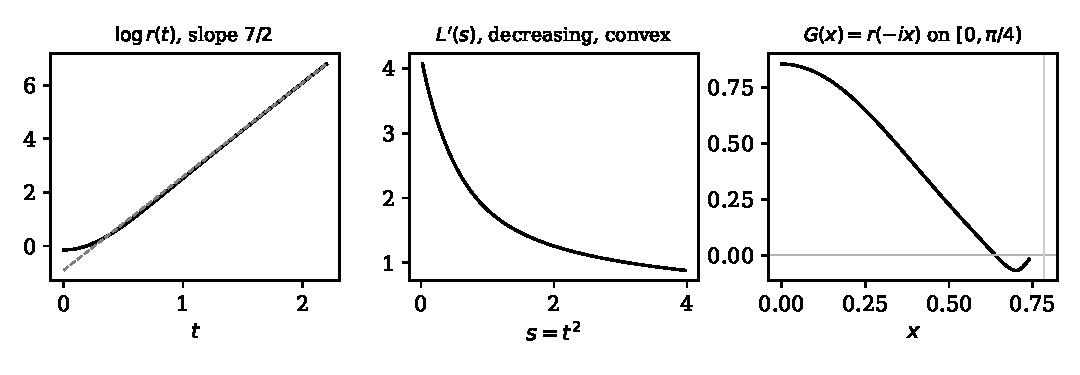
\includegraphics[width=\textwidth]{rzfig/fig_cardon.pdf}
\caption{The Cardon ratio for the random harmonic law $H_{\kappa^*}$. Left: $\log r(t)$ on the real axis, asymptotically linear with slope $\frac72$ (dashed). Centre: $L'(s)$ for $L(s)=\log(r(\sqs)/r(0))$, positive, decreasing and convex as a Stieltjes function must be. Right: the continuation $G(x)=r(-ix)$ on $[0,\pi/4)$, with a simple zero at $x=0.6388$.}
\label{rz:fig:cardon}
\end{figure}

\begin{proposition}\label{rz:prop:cardonnum}
The ratio $r$ satisfies the following necessary conditions for \eqref{rz:eq:cardonrep} (computed).
\begin{enumerate}
\item[(i)] Growth. $r$ is even, $r(0)=0.853936$, and $\log r(t)$ becomes linear with slope approaching $\frac72$: the increments over steps of $0.1$ fall from $0.3534$ to $0.3514$ between $t=1.5$ and $t=2.2$. The slope is explained exactly: $\Phi$ carries the prefactor $e^{9t/2}$, and the saddle point prefactor $\sqrt{s^*/\pi}\approx e^{t}$ of $f_{\kappa^*}$ removes one unit. So $G$ would have exponential type $\frac72$, compatible with order one.
\item[(ii)] Stieltjes signs. With $L(s)=\log r(\sqs)-\log r(0)$, a Laguerre P\'olya $G$ requires $L'(s)=\sum m_k/(s+\alpha_k^2)$, a Stieltjes function. On a grid of $81$ points in $s\in[0,4]$ the difference quotients of $L$ give $L'>0$, $L''<0$ and $L'''>0$ everywhere, and the first order quotients fall from $4.07$ on the first grid interval to $0.94$ on the last.
\item[(iii)] The imaginary axis. The continuation $G(x)=r(-ix)$, computed independently from $\Phi(ix)$ and $f_{\kappa^*}(ix)$, is real, agrees with $r$ at second order ($\log(G(0.1)/G(0))=-0.0423$ against $\log(r(0.1)/r(0))=0.0417$), decreases from $0.8539$, has a simple zero at $\alpha_1=0.6388$, and satisfies the Laguerre inequality $G'^2-GG''\ge2.4>0$ on $[0,0.735]$.
\end{enumerate}
\end{proposition}

Everything visible inside the strip is consistent with $G$ being a Laguerre P\'olya function of exponential type $\frac72$: the single zero $\alpha_1$ accounts for $1/\alpha_1^2=2.45$ of the curvature $\sum m_k/\alpha_k^2\approx4.2$, and a zero density of about $\frac7{2\pi}$ per unit beyond it would account for the linear growth. The decisive question cannot be settled inside the strip.

\begin{proposition}\label{rz:prop:boundary}
If \eqref{rz:eq:cardonrep} holds with $G$ entire, then
\[
f_{\kappa^*}(t)=\Phi(t)/(\Xi(0)G(it)),
\]
so $f_{\kappa^*}$ continues meromorphically exactly as far as $\Phi$ does, and the two share their singular behaviour on the lines $\Im t=\pm\pi/4$, apart from the zeros of $G$. Since $\Phi$ has a natural boundary on these lines, coming from the Jacobi theta function at the edge of its modular domain, $f_{\kappa^*}$ must have the same natural boundary, with singular behaviour proportional to that of $\Phi$ through a factor that continues to an entire function.
\end{proposition}

The first sentence of Proposition~\ref{rz:prop:boundary} is immediate. The second uses the classical fact that the theta function $\omega(x)=\sum_{n\ge1}e^{-\pi n^2x}$ has the line $\Re x=0$ as a natural boundary \cite[Chapter~11, Section~1.4, and Chapter~5, Section~3.2]{Remmert98}, together with $\Phi(t)=4x^{9/4}\omega''(x)+6x^{5/4}\omega'(x)$ at $x=e^{2t}$. Nothing is proved here about whether $f_{\kappa^*}$ has such a boundary; the proposition records what \eqref{rz:eq:cardonrep} would require.

So the random harmonic law fits the P\'olya kernel inside the strip, and the question is the boundary, where the two functions have different origins: $\Phi$ is a modular theta series and $f_{\kappa^*}$ a Rademacher product whose characteristic function has real zeros at $v=(2j+1)\pi(k+\kappa^*)$, increasingly dense. For \eqref{rz:eq:cardonrep} to hold, the Rademacher product would have to reproduce the modular singularities of $\Phi$ up to an entire factor. We see no reason for that, and it suggests that the right Ising system for the P\'olya variable is not the harmonic paramagnet but one whose magnetisation law carries theta function structure.

\subsubsection{The P\'olya variable as the logarithm of a GGC}

Proposition~\ref{rz:prop:boundary} asks for a Lee and Yang system whose magnetisation law carries the modular boundary of $\Phi$. Jacobi's triple product is the first candidate, since it writes a theta function as the characteristic function of a sum of independent two point variables, but these are not Lee and Yang spins (Proposition~\ref{rz:prop:jtp}); the modular structure turns out to live in a multiplicative magnetisation.

\begin{proposition}\label{rz:prop:jtp}
For $0<q<1$ the triple product
\[
\sum_{n\in\mathbb Z}q^{n^2}e^{inv}=\prod_{m\ge1}(1-q^{2m})\bigl(1+2q^{2m-1}\cos v+q^{4m-2}\bigr)
\]
exhibits the discrete Gaussian law $\Pr(J=n)\propto q^{n^2}$ as the law of $\sum_m(B_m-B_m')$ with independent Bernoulli variables of parameter $q^{2m-1}/(1+q^{2m-1})$. Each factor vanishes at $v=\pi\pm i(2m-1)\log(1/q)$, so the characteristic function has no real zeros and the moment generating function has no purely imaginary zeros: the triple product spins are not Lee and Yang spins, and neither is the discrete Gaussian.
\end{proposition}

\begin{proof}
$1+2q^{2m-1}\cos v+q^{4m-2}=(1+q^{2m-1}e^{iv})(1+q^{2m-1}e^{-iv})$, and each factor, normalised, is the characteristic function of a Bernoulli variable or its negative. The zeros are those of $1+q^{2m-1}e^{\pm iv}$.
\end{proof}

So the triple product places the theta function in the field variable, where its zeros lie on horizontal lines rather than on the real axis. For $\Phi$ the theta function enters through the modular variable $e^{2t}$, and the relevant structure is multiplicative. Recall from Section~\ref{ch:clock} the identity of Biane, Pitman and Yor \cite{BPY01}, going back to Williams \cite{Williams90}, which makes this exact.

\begin{theorem}\label{rz:thm:bpy}
Let $S_2=\sum_{k\ge1}\frac{2}{\pi^2k^2}(e_k+e_k')$ with independent standard exponentials $e_k,e_k'$, so that $\E e^{-sS_2}=\bigl(\sqrt{2s}/\sinh\sqrt{2s}\bigr)^2$ and $S_2$ is a GGC with Thorin measure $2\sum_k\delta_{\pi^2k^2/2}$. Then
\[
2\xi(z)=\E\Bigl[\Bigl(\frac{\pi S_2}2\Bigr)^{z/2}\Bigr].
\]
Consequently, with $Y=\frac12\log(\pi S_2/2)$, $2\Xi(\tau)=\E[e^{Y/2}e^{i\tau Y}]$, and the P\'olya variable $X$ is $Y$ tilted by $e^{Y/2}$: $\Phi(t)\,dt=\frac12e^{t/2}\,\Pr(Y\in dt)$.
\end{theorem}

\begin{proof}
This is the identity of \cite[Section~2]{BPY01}; the density of $S_2$ is a theta series by the partial fraction expansion of $(x/\sinh x)^2$ and Poisson summation, and its Mellin transform is $2\xi$.
\end{proof}

We checked the identity exactly at $z=2$ and $z=4$, where $\E S_2=\frac23$ and $\E S_2^2=\frac8{15}$ give $\frac\pi3=2\xi(2)$ and $\frac{2\pi^2}{15}=2\xi(4)$, and numerically at $z=0.8+3i$, where both sides equal $0.8073665638+0.0340962268i$ to ten digits, using $\E V^w=\frac{w}{\Gamma(1-w)}\int_0^\infty s^{-w-1}(1-\E e^{-sV})\,ds$ for positive $V$ and $0<\Re w<1$. Table~\ref{bp:tab:bpy} in Section~\ref{ch:basepoint} checks the identity by simulation at real arguments, and Section~\ref{bp:sec:mellin} there tilts $Y$ to every real basepoint $\sigma$: with no hypothesis, $\xi(\sigma+z)/\xi(\sigma)$ is the moment generating function of $\frac12\log(\frac\pi2S_2)$ under the law of $S_2$ size biased by $S_2^{\sigma/2}$.

Theorem~\ref{rz:thm:bpy} shows where the modular boundary comes from. The P\'olya variable is a tilted logarithm of a GGC whose Thorin atoms lie on the quadratic lattice $\pi^2k^2/2$, and it is the quadratic lattice, through Jacobi's theta function and Poisson summation, that produces the modular natural boundary at $\Im t=\pm\pi/4$: the density of $S_2$ is analytic in $\Re x>0$ with natural boundary on $\Re x=0$, and $x=\frac2\pi e^{2t}$. The Thorin structure thus enters twice: $R$ is the reciprocal moment generating function of the P\'olya variable in $\sqs$, and $S_2$ is a GGC in the usual sense. RH is the statement that every zero of $w\mapsto\E[(\pi S_2/2)^w]$ in the strip $0<\Re w<\frac12$ lies on the line $\Re w=\frac14$.

This suggests a multiplicative Lee and Yang property. We say that a positive random variable $V$ has \emph{Mellin zeros on a line} if $\E V^{w}$, continued, vanishes only on one vertical line. The solved models of the Vere-Jones step have exact multiplicative analogues.

\begin{proposition}\label{rz:prop:multlee}
Let $V=\sum_{k\le n}c_ke_k$ with independent standard exponentials $e_k$ and distinct $c_k>0$. Then $\E V^{u-1}=\Gamma(u)\sum_kA_kc_k^{u}$ with $A_k=c_k^{n-2}/\prod_{j\ne k}(c_k-c_j)$.
\begin{enumerate}
\item[(i)] For $n=2$ the zeros are $u=2\pi i m/\log(c_1/c_2)$, $m\ne0$: all on the line $\Re u=0$. The two exponential sum is a multiplicative solved model.
\item[(ii)] For $n=3$ with $c=(1,\frac14,\frac19)$, a truncation of the quadratic lattice with single atoms, the zeros in $0<\Im u<30$ have real parts $0.488$, $-1.268$, $0.300$, $0.387$, $-1.318$, $0.457$, $0.136$, $-1.129$, $0.500$ (computed): they do not lie on a line.
\end{enumerate}
\end{proposition}

\begin{proof}
The density of $V$ is $\sum_kA_ke^{-x/c_k}$ by partial fractions of $\prod_k(1+c_ks)^{-1}$, and its Mellin transform is the stated exponential polynomial times $\Gamma(u)$. For $n=2$ it is proportional to $c_1^u-c_2^u$. For $n=3$ the zeros are those of $1.5-2.4\cdot4^{-u}+0.9\cdot9^{-u}$, which has none with $|\Re u|\ge8$; the argument principle on $[-8,8]\times[0.01,30]$ counts nine, none lies in $0<\Im u<0.01$, and Newton's method locates them at $0.4881+4.4641i$, $-1.2675+7.6319i$, $0.2997+9.2799i$, $0.3865+13.4112i$, $-1.3178+15.5448i$, $0.4570+18.2547i$, $0.1355+22.4710i$, $-1.1294+23.3902i$ and $0.4998+27.1862i$.
\end{proof}

So the Lee and Yang mechanism survives the passage from additive to multiplicative magnetisations for two components and fails at three, just as a sum of two cosines has real zeros while a generic sum of three need not.

\section{Truncations, finite conditions and the road to RH}\label{ch:rz4}

Cutting the series for $S_2$ in Theorem~\ref{rz:thm:bpy} after $n$ terms gives variables whose Mellin transforms are explicit, each a gamma factor times an exponential polynomial, with zeros that converge to the points $\rho/2$; a condition on these zeros, holding for infinitely many $n$, implies RH. We follow this route to the point where it stops. The one sided condition fails because the truncated zeros approach the critical line from a side fixed by an explicit constant $\kappa(\rho)$, and the side changes at zeros where $|S(\gamma)|$ is large, with $S(t)=\pi^{-1}\arg\zeta(\frac12+it)$ as in Appendix~\ref{app:notation}; the first such zero is $\gamma_{213}$. Symmetrising by the functional equation removes this mechanism. The resulting Conjecture S is proved above explicit heights for $n\le6$ and $n=8$ and checked numerically below them; for the other $n\le24$ and for $n=32,36$ it follows above explicit heights from torus bounds proved in ball arithmetic, and is checked numerically below them. Section~\ref{rz:sec:towards} sets the reductions of Chapter~\ref{chap:rzeta} and of this chapter against what is proved unconditionally: Weil's criterion in Thorin coordinates, Weil positivity on the Bernstein cone, the reach of finite order tests, the de Bruijn Newman flow and GGC multipliers. Sections~\ref{rz:sec:num}, \ref{rz:sec:disc} and \ref{rz:sec:open} record the numerical verification of both chapters, say what their results mean for the Thorin approach, and state open problems.

\subsection{Truncations of the Biane, Pitman and Yor lattice}\label{rz:sec:finite}

In this subsection $w$ is the complex variable of a Mellin transform and $u=w+1$; the canonical function $w(x)$ of Theorem~\ref{rz:thm:w} does not return until Section~\ref{rz:sec:towards}. The results are of three kinds. The Hurwitz reductions, the first order expansion of the truncated zeros, the formula for its constant and the single term bound for small $n$ are theorems. The argument principle counts are computations in floating point. Corollary~\ref{rz:cor:Tfalse} rests in addition on an enclosure of $\Re\kappa(\rho_{213})$ in ball arithmetic, and the results for $n=7$, $9\le n\le24$ and $n=32,36$ on bounds over a torus, proved by a branch and bound whose final boxes are enclosed in ball arithmetic.

\subsubsection{Truncated lattices and Conjecture T}

Let $e_k,e_k'$ be independent standard exponential variables, and put $\mathcal S=\sum_{k\ge1}k^{-2}(e_k+e_k')=\frac{\pi^2}2S_2$, with $S_2$ the variable of Theorem~\ref{rz:thm:bpy}, and $\mathcal S_n=\sum_{k\le n}k^{-2}(e_k+e_k')$, a GGC with finitely many Thorin atoms. Put $F(w)=\E\mathcal S^w$ and $F_n(w)=\E\mathcal S_n^w$ for $\Re w>-2$. By Theorem~\ref{rz:thm:bpy},
\[
F(w)=2\pi^{w}\,\xi(2w),
\]
so the zeros of $F$ are the points $w=\rho/2$, and RH says they lie on $\Re w=\frac14$. Each $F_n$ is explicit. Define $\alpha_k$ and $\beta_k$, which depend on $n$, by the partial fraction expansion
\[
\prod_{j\le n}\Bigl(1+\frac\lambda{j^2}\Bigr)^{-2}=\sum_{k\le n}k^{-2}\Bigl\{\alpha_k\Bigl(1+\frac\lambda{k^2}\Bigr)^{-1}+\beta_k\Bigl(1+\frac\lambda{k^2}\Bigr)^{-2}\Bigr\},
\]
so that $\beta_k=k^2\prod_{j\le n,\,j\ne k}(1-k^2/j^2)^{-2}$ and $\alpha_k=-2\beta_k\sum_{j\le n,\,j\ne k}k^2/(j^2-k^2)$; for $n=2$ they are $\beta=(\frac{16}9,\frac49)$ and $\alpha=(-\frac{32}{27},\frac{32}{27})$. The left side is the Laplace transform of $\mathcal S_n$, whose density is therefore $\sum_k(\alpha_k+\beta_kk^2x)e^{-k^2x}$, and taking moments gives, with $u=w+1$, $F_n(u-1)=\Gamma(u)Q_n(u)$, where $Q_n(u)=\sum_{k\le n}k^{-2u}(\alpha_k+\beta_ku)$. So $F_n$ is, up to $\Gamma$, an exponential polynomial with frequencies $2\log k$ and coefficients linear in $u$.

\begin{theorem}\label{rz:thm:hurwitzrh}
If for infinitely many $n$ the function $F_n$ has no zeros in the half plane $\Re w>\frac14$, then the Riemann Hypothesis holds.
\end{theorem}

\begin{proof}
For $\Re w>-2$ the variables $\mathcal S_n^w$ are dominated by an integrable variable, since $\mathcal S_n\ge e_1+e_1'$ and $\mathcal S_n\le\mathcal S$, so $F_n\to F$ locally uniformly on $\Re w>-2$. If $F$ had a zero $w_0$ with $\Re w_0>\frac14$, Hurwitz's theorem would give zeros of $F_n$ near $w_0$ for all large $n$. Hence every zero $\rho/2$ of $F$ has $\Re\rho\le\frac12$, and the symmetry $\rho\mapsto1-\rho$ gives $\Re\rho=\frac12$.
\end{proof}

Asking for the hypothesis at every $n$ gives the simplest condition of this kind.

\medskip
\noindent\textsc{Conjecture T.} For every $n\ge1$, $F_n(w)=\E\bigl[\bigl(\sum_{k\le n}k^{-2}(e_k+e_k')\bigr)^w\bigr]$ has no zeros with $\Re w>\frac14$.
\medskip

By Theorem~\ref{rz:thm:hurwitzrh}, Conjecture T implies RH. It is a stability statement, of Hermite Biehler or Lee and Yang type \cite{LeeYang}, for a sequence of explicit exponential polynomials. It is false (Corollary~\ref{rz:cor:Tfalse}, whose proof uses an enclosure of $\Re\kappa(\rho_{213})$ in ball arithmetic), and we state it because the mechanism of its failure also defeats, for large $n$, the Hermite Biehler inequality on which the bounds of Theorems~\ref{rz:thm:Yn} and \ref{rz:thm:torus} for the symmetrised truncations rest.

At small $n$ the evidence supports it: Table~\ref{rz:tab:Trect} finds no zero of $Q_n$ with $\Re u>\frac54$ in any rectangle searched. The zeros are counted by the argument principle, with $800$ to $4000$ sample points per side and a working precision of $40$ to $340$ decimal digits to control the cancellation among the partial fraction coefficients, and located by Newton's method from a grid; the counts and the zeros found agree.

\begin{table}[htbp]
\centering
\small
\begin{tabular}{lll}
\toprule
$n$ & region, in $u=w+1$ & zeros with $\Re u>\frac54$\\
\midrule
$2,3,4,5,6,8,12,16,24,32$ & $\frac54<\Re u<6$, $0.3<\Im u<40$ & none\\
$8,16,32$ & $\frac54<\Re u<6$, $40<\Im u<100$ & none\\
$48,64$ & $\frac54<\Re u<6$, $0.3<\Im u<30$ & none\\
$16,32,64$ & $6<\Re u<40$, $0.3<\Im u<40$ & none\\
\bottomrule
\end{tabular}
\caption{Argument principle counts for Conjecture T: rectangles searched and zeros of $Q_n$ found with $\Re u>\frac54$.}
\label{rz:tab:Trect}
\end{table}

Rectangles to the left of the line contain the expected zeros: $8$, $12$, $12$, $15$, $15$, $17$, $18$, $19$, $21$, $21$ zeros with $-6<\Re u<\frac54$ and $\Im u<40$ for the ten values of $n$ in the first row. For $n=2$ the eight zeros found lie on $\Re u=-1$ exactly. On the real axis $F_n$ is positive, and for fixed $n$ and large $|\Im u|$ the zeros move far to the left, because the extreme coefficients $\beta_1$ and $\beta_n$ differ by a factor of order $16^n$, up to a power of $n$. The intermediate heights are therefore where Conjecture T is at risk, and they are the heights that Table~\ref{rz:tab:Trect} searches; the failure found in Corollary~\ref{rz:cor:Tfalse} lies above them (Remark~\ref{rz:rem:firstordergap}). An experiment shows that the absence of such zeros at small $n$ is not a consequence of the GGC structure alone: replacing the weights $k^{-2}$ by $k^{-2}(1+\eta_k)$, with independent $\eta_k$ uniform on $[-0.15,0.15]$, one of two draws at $n=16$ gives a zero with $\Re u>\frac54$. The property depends on the exact quadratic lattice.

\subsubsection{How the truncated zeros reach the line, and why Conjecture T fails}

Near a simple zero $\rho$ of $\xi$, the zeros of $F_n$ converge to $\rho/2$ at rate $1/n$, with an explicit constant.

\begin{proposition}\label{rz:prop:firstorder}
Let $\rho$ be a simple zero of $\xi$ and put
\[
\kappa(\rho)=\frac{\rho\,\xi(\rho-2)}{2\pi\,\xi'(\rho)}=\frac{\rho\,\xi(3-\rho)}{2\pi\,\xi'(\rho)} .
\]
There is a constant $C$ such that for all large $n$, $F_n$ has exactly one zero $w_n(\rho)$ in the disc $|w-\frac\rho2-\frac{\kappa(\rho)}n|<C/n^2$; thus $w_n(\rho)=\frac\rho2+\frac{\kappa(\rho)}n+O(n^{-2})$.
\end{proposition}

\begin{proof}
Write $\mathcal S=\mathcal S_n+\mathcal T_n$ with $\mathcal T_n=\sum_{k>n}k^{-2}(e_k+e_k')$, independent of $\mathcal S_n$, so that $\E\mathcal T_n=2\sum_{k>n}k^{-2}=\frac2n+O(n^{-2})$ and $\E\mathcal T_n^2=O(n^{-2})$. For $a>0$, $b\ge0$ and $0<\Re w<2$, Taylor's formula with integral remainder and $|(a+tb)^{w-2}|=(a+tb)^{\Re w-2}\le a^{\Re w-2}$ give
\begin{gather*}
\bigl|(a+b)^w-a^w-wb\,a^{w-1}\bigr|\le\tfrac12|w(w-1)|\,b^2a^{\Re w-2},\\
\bigl|(a+b)^{w-1}-a^{w-1}\bigr|\le|w-1|\,b\,a^{\Re w-2}.
\end{gather*}
Since $\mathcal S_n\ge e_1+e_1'$, a $\Gamma(2)$ variable, $\E\mathcal S_n^{\Re w-2}\le\Gamma(\Re w)$. Taking expectations with $a=\mathcal S_n$ and $b=\mathcal T_n$, and using independence,
\[
F(w)=F_n(w)+w\,\E\mathcal T_n\,F_n(w-1)+O(n^{-2}),\qquad F_n(w-1)=F(w-1)+O(n^{-1}),
\]
uniformly on compact subsets of $0<\Re w<2$. Hence $F_n(w)=F(w)-\frac2nwF(w-1)+O(n^{-2})$ uniformly there. Put $w_0=\rho/2$, so $0<\Re w_0<\frac12$, and recall $F(w_0)=0$ and $F'(w_0)=4\pi^{w_0}\xi'(\rho)\ne0$. For $|w-w_0|=O(1/n)$, Taylor expansion of $F$ and of $wF(w-1)$ about $w_0$ gives
\[
F_n(w)=F'(w_0)\Bigl(w-w_0-\frac{\kappa(\rho)}n\Bigr)+O(n^{-2}),\qquad\frac{\kappa(\rho)}n=\frac2n\,\frac{w_0F(w_0-1)}{F'(w_0)},
\]
and $F(w_0-1)=2\pi^{w_0-1}\xi(\rho-2)$ turns the second identity into the stated $\kappa$. On the circle $|w-w_0-\kappa/n|=C/n^2$ the linear term has modulus $|F'(w_0)|C/n^2$, which exceeds the $O(n^{-2})$ error once $C$ is larger than its constant divided by $|F'(w_0)|$. Rouch\'e's theorem gives exactly one zero inside for all large $n$. The second form of $\kappa$ follows from $\xi(s)=\xi(1-s)$.
\end{proof}

Each simple zero $\rho$ of $\xi$ thus has a companion zero of the truncation at distance of order $1/n$, displaced in the direction $\kappa(\rho)$. If $\Re\kappa(\rho)>0$ the companion lies to the right of the critical line for all large $n$. This happens at zeros where $|S(\gamma)|$ is large, the first being $\gamma_{213}$ (Theorem~\ref{rz:thm:kappaexact} and the computation after it), and it is why Conjecture T fails.

For each of the first $100$ zeros $\kappa(\rho)$ has negative real part, starting with $\kappa(\rho_1)=-4.762-1.944i$, $\kappa(\rho_2)=-8.673-0.627i$, $\kappa(\rho_3)=-10.149-3.872i$ and $\kappa(\rho_4)=-15.165+3.705i$. So these truncated zeros approach the critical line from the left, at distance about $-\Re\kappa(\rho)/n$, which grows with the height: $-\Re\kappa(\rho)/\gamma^2$ lies between $0.011$ and $0.024$ for the first ten zeros, with $0.024$ at $\gamma_1$ and $0.013$ at $\gamma_{10}$. Figure~\ref{rz:fig:traj} and Table~\ref{rz:tab:traj} show the approach for the first four zeros, computed by locating the zeros of $F_n$ directly at each $n$ rather than from the expansion. The convergence of $n(\frac54-\Re u)$ to $-\Re\kappa(\rho_j)$, in the right panel of the figure and the last row of the table, is an independent check on Proposition~\ref{rz:prop:firstorder} at low height.

\begin{figure}[htbp]
\centering
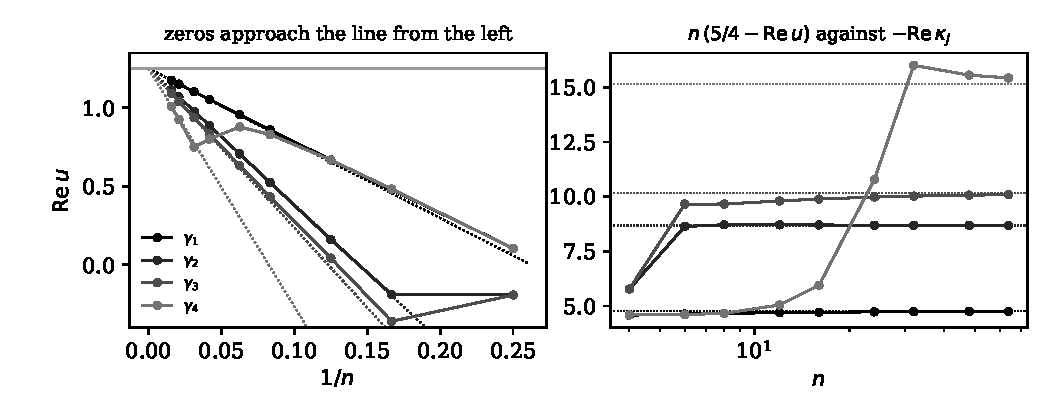
\includegraphics[width=0.95\textwidth]{rzfig/fig_traj.pdf}
\caption{Left: real parts of the zeros of $F_n$ near $\rho_j/2$, in the variable $u=w+1$, against $1/n$ for $n=4$ to $64$, with the first order lines $\frac54+\Re\kappa(\rho_j)/n$ (dotted). The zeros approach $\Re u=\frac54$, the image of the critical line, from the left. Right: $n(\frac54-\Re u)$ against $n$, converging to $-\Re\kappa(\rho_j)$.}
\label{rz:fig:traj}
\end{figure}

\begin{table}[htbp]
\centering
\footnotesize
\setlength{\tabcolsep}{4pt}
\begin{tabular}{rcccc}
\toprule
$n$ & near $\rho_1/2$ & near $\rho_2/2$ & near $\rho_3/2$ & near $\rho_4/2$\\
\midrule
$8$ & $0.6678+6.8583i$ & $0.1610+10.6538i$ & $0.0426+11.9969i$ & $0.6676+15.7727i$\\
$16$ & $0.9558+6.9550i$ & $0.7062+10.5197i$ & $0.6321+12.2722i$ & $0.8787+15.7928i$\\
$32$ & $1.1020+7.0090i$ & $0.9785+10.5029i$ & $0.9368+12.3881i$ & $0.7498+15.4606i$\\
$64$ & $1.1758+7.0376i$ & $1.1144+10.5040i$ & $1.0924+12.4460i$ & $1.0089+15.2948i$\\
limit & $1.25+7.0674i$ & $1.25+10.5110i$ & $1.25+12.5054i$ & $1.25+15.2124i$\\
$n(\frac54-\Re u)$ at $64$ & $4.75$ & $8.68$ & $10.09$ & $15.43$\\
\bottomrule
\end{tabular}
\caption{Zeros of $F_n$ near $\rho_j/2$, in the variable $u=w+1$. The row ``limit'' is $\rho_j/2+1$; the last row, $n(\frac54-\Re u)$ at $n=64$, is to be compared with $-\Re\kappa(\rho_j)=4.762$, $8.673$, $10.149$, $15.165$.}
\label{rz:tab:traj}
\end{table}

The direction from which a truncated zero reaches the line is not always the same, and the sign of $\Re\kappa(\rho)$ can be read off from Hardy's function.

\begin{theorem}\label{rz:thm:kappaexact}
Let $\rho=\frac12+i\gamma$ be a simple zero on the critical line, let $\theta$ be the Riemann Siegel theta function and $Z(t)=e^{i\theta(t)}\zeta(\frac12+it)$ Hardy's function, and put $a(\gamma)=e^{i\theta(\gamma)}\zeta(\frac52+i\gamma)$. Then
\begin{align*}
\Re\kappa(\rho)&=\frac{(\gamma^2-\frac{15}4)\Im a(\gamma)-4\gamma\Re a(\gamma)}{4\pi^2Z'(\gamma)},\\
\Im\kappa(\rho)&=\frac{4\gamma\Im a(\gamma)+(\gamma^2-\frac{15}4)\Re a(\gamma)}{4\pi^2Z'(\gamma)} .
\end{align*}
\end{theorem}

\begin{proof}
On the line $\xi(\frac12+it)=\Xi(t)$ is real, so $\xi'(\rho)=-i\,\Xi'(\gamma)$, and $\Xi(t)=-\frac12(t^2+\frac14)\pi^{-1/4}|\Gamma(\frac14+\frac{it}2)|Z(t)$ gives $\Xi'(\gamma)=-\frac12(\gamma^2+\frac14)\pi^{-1/4}|\Gamma(\frac14+\frac{i\gamma}2)|Z'(\gamma)$ at a zero. Since $\xi(3-\rho)=\xi(\frac52-i\gamma)$ and $\xi$ is real on the real axis, $\xi(3-\rho)=\overline{\xi(\frac52+i\gamma)}$, and $\Gamma(\frac54+\frac{i\gamma}2)=(\frac14+\frac{i\gamma}2)\Gamma(\frac14+\frac{i\gamma}2)$ with $\pi^{-i\gamma/2}\Gamma(\frac14+\frac{i\gamma}2)=|\Gamma(\frac14+\frac{i\gamma}2)|e^{i\theta(\gamma)}$. Substituting, the moduli of $\Gamma$ cancel, $(\frac12+i\gamma)(\frac14-\frac{i\gamma}2)=\frac12(\gamma^2+\frac14)$ cancels the remaining factor, and $\kappa=-i(\frac52-i\gamma)(\frac32-i\gamma)\overline{a(\gamma)}/(4\pi^2Z'(\gamma))$, whose real and imaginary parts are as stated.
\end{proof}

For large $\gamma$ the term $(\gamma^2-\frac{15}4)\Im a(\gamma)$ decides the sign of $\Re\kappa(\rho)$. Since $|\zeta(\frac52+i\gamma)-1|\le\zeta(\frac52)-1<0.35$, $a(\gamma)$ is a positive multiple of $e^{i\theta(\gamma)}$ up to a phase below $0.35$ in modulus, and up to that phase the sign of $\Re\kappa(\rho)$ is the sign of $\sin\theta(\gamma)/Z'(\gamma)$. Let $S_{\rm mid}$ be the midpoint of the jump of $S$ at the $n$th zero $\gamma_n$. Then $\theta(\gamma_n)=\pi(n-\frac32-S_{\rm mid})$ and the sign of $Z'(\gamma_n)$ is $(-1)^{n+1}$, so the sign of $\sin\theta(\gamma_n)/Z'(\gamma_n)$ is that of $-\cos(\pi S_{\rm mid})$: negative when $|S_{\rm mid}|<\frac12$, that is when the zero lies within half a spacing of its expected position, and positive when $\frac12<|S_{\rm mid}|<\frac32$. The phase of $\zeta(\frac52+i\gamma)$ moves the threshold $\frac12$ by at most about $0.11$ either way. For the first $460$ zeros the sign of $\Re\kappa$ agrees with the sign of $\Im a(\gamma)/Z'(\gamma)$ in every case, and $\Re\kappa>0$ occurs three times, at
\[
\gamma_{213}=415.4552,\quad\gamma_{289}=527.9036,\quad\gamma_{379}=650.6687,
\]
with $\kappa=233.96-2298.91i$, $604.16+3074.08i$, $1164.60-4296.91i$.

At these three zeros the jump of $S$ runs from $0.098$ to $1.098$, from $-1.145$ to $-0.145$ and from $0.164$ to $1.164$; the midpoints of the jumps are $0.598$, $-0.645$ and $0.664$. Seven of the first $460$ zeros have $S(\gamma^-)<-1$: besides $\gamma_{289}$ these are $\gamma_{127}$, $\gamma_{196}$, $\gamma_{233}$, $\gamma_{368}$, $\gamma_{380}$ and $\gamma_{401}$, with midpoints $-0.506$, $-0.505$, $-0.537$, $-0.556$, $-0.538$ and $-0.514$, and $\Re\kappa$ is negative at every one of them. Three further zeros have midpoints above $\frac12$ and $\Re\kappa<0$: $\gamma_{136}$, $\gamma_{256}$ and $\gamma_{399}$, at $0.507$, $0.510$ and $0.539$. The largest $|S_{\rm mid}|$ with $\Re\kappa<0$ is $0.556$, at $\gamma_{368}$, and the smallest with $\Re\kappa>0$ is $0.598$, at $\gamma_{213}$, so the threshold on the midpoint lies between about $0.56$ and $0.60$, inside the range $\frac12\pm0.11$ allowed by the phase of $\zeta(\frac52+i\gamma)$.

\begin{corollary}\label{rz:cor:Tfalse}
Conjecture T is false: for all sufficiently large $n$, $F_n$ has a zero with $\Re w>\frac14$ near $\rho_{213}/2$.
\end{corollary}

\begin{proof}
The first $1.5\times10^9$ zeros, $\rho_{213}$ among them, lie on the critical line and are simple \cite{LRW86}, and ball arithmetic applied to the formula of Theorem~\ref{rz:thm:kappaexact} gives $233.95<\Re\kappa(\rho_{213})<233.96$ (Section~\ref{rz:sec:num}). By Proposition~\ref{rz:prop:firstorder}, for all large $n$ the function $F_n$ has a zero $w_n$ with $|w_n-\frac{\rho_{213}}2-\frac{\kappa(\rho_{213})}n|<C/n^2$, so $\Re w_n>\frac14+\frac{233.95}n-\frac C{n^2}>\frac14$ once $n>C/233.95$.
\end{proof}

In particular the hypothesis of Theorem~\ref{rz:thm:hurwitzrh} fails for every large $n$.

\begin{remark}\label{rz:rem:firstordergap}
The constants in Proposition~\ref{rz:prop:firstorder} depend on $\rho$, and the first order regime requires $n$ large compared with $|\kappa(\rho)|$. For the zero $\rho_{213}$ of Corollary~\ref{rz:cor:Tfalse}, $|\kappa(\rho_{213})|=2311$, so the phenomenon begins at $n$ of order $10^3$ or beyond, larger than every $n$ computed in this section. Table~\ref{rz:tab:Trect} accordingly reports no zero with $\Re u>\frac54$, and cannot detect this one, since its rectangles reach $\Im u=100$ while the predicted failure sits at $\Im u=207.7$.
\end{remark}

The failure is intrinsic to the method, not to the particular lattice. Any truncation whose first order error is a multiple of $F(w-1)$ produces the displacement $\kappa(\rho)/n$, and the phase of $\kappa(\rho)$ is governed by $S(\gamma)$. By Selberg's central limit theorem \cite{Selberg46} $S$ takes values beyond $\pm\frac12$ for a positive proportion of heights, so one expects a positive proportion of zeros to be approached from the right. One sided Hurwitz arguments therefore cannot succeed for truncations of this kind; what is needed is a scheme in which symmetry keeps the zeros on the line.

\subsubsection{Symmetrised truncations and Conjecture S}

The functional equation supplies that symmetry. Put
\[
K_n(w)=\pi^{-w}F_n(w)+\pi^{w-\frac12}F_n(\tfrac12-w),\qquad Z_n(y)=K_n(\tfrac14+iy).
\]

\begin{proposition}\label{rz:prop:symtrunc}
$K_n(\frac12-w)=K_n(w)$, $K_n(\bar w)=\overline{K_n(w)}$, so $Z_n$ is real for real $y$ and the zeros of $K_n$ off the line $\Re w=\frac14$ come in quadruples. As $n\to\infty$, $K_n\to4\,\xi(2w)$ locally uniformly on $-\frac74<\Re w<\frac94$. Every simple zero $\frac14+i\frac\gamma2$ of $\xi(2w)$ on the line is, for all large $n$, the limit of a zero of $K_n$ lying exactly on the line.
\end{proposition}

\begin{proof}
The symmetries are immediate from the definition and the reality of $F_n$ on the real axis. The limit follows from $F_n\to F=2\pi^w\xi(2w)$ and $\xi(1-2w)=\xi(2w)$; since $F_n\to F$ on $\Re w>-2$, the convergence holds on $-2<\Re w<\frac52$, which contains the strip of the statement. Near a simple zero $y_0$ of the real function $4\xi(\frac12+2iy)$, $Z_n$ converges uniformly and so changes sign near $y_0$; by Hurwitz, $K_n$ has exactly one zero near $\frac14+iy_0$, which must be the real zero of $Z_n$, since an off line zero would bring its mirror image $\frac12-\bar w$ with it.
\end{proof}

So for symmetrised truncations the local mechanism that broke Conjecture T is absent: a simple zero on the line cannot leave it under a small symmetric perturbation; it can leave only after colliding with another zero. The Hurwitz argument now gives the following.

\begin{theorem}\label{rz:thm:symhurwitz}
If for infinitely many $n$ all zeros of $K_n$ in the strip $0<\Re w<\frac12$ lie on the line $\Re w=\frac14$, then RH holds.
\end{theorem}

\begin{proof}
A zero $\rho/2$ of $\xi(2w)$ off the line lies in the strip $0<\Re w<\frac12$, since $0<\Re\rho<1$, and by Hurwitz it is the limit of zeros of $K_n$ in the strip, which would be off the line for large $n$.
\end{proof}

\medskip
\noindent\textsc{Conjecture S.} For every $n\ge1$, all zeros of $K_n$ in $0<\Re w<\frac12$ lie on $\Re w=\frac14$.
\medskip

The symmetrised zeros move along the line. The first order argument of Proposition~\ref{rz:prop:firstorder}, applied to $K_n=2\Re[\pi^{-w}F_n(w)]$ on the line, gives
\[
w_n^{\mathrm{sym}}(\rho)=\frac\rho2+\frac{i\,\Im\kappa(\rho)}n+O(n^{-2}):
\]
the symmetrisation removes the real part of the displacement, which is the part that broke Conjecture T, and keeps the imaginary part. Numerically the first two symmetrised zeros are at $\Im w=7.0328,7.0072,7.0231,7.0413$ and $10.5490,10.5392,10.5161,10.5085$ for $n=8,16,32,64$, against the first order values $7.0370$ and $10.5012$ at $n=64$.

\begin{table}[htbp]
\centering
\small
\begin{tabular}{llll}
\toprule
$n$ & window in $\Im w$ & \begin{tabular}[b]{@{}l@{}}zeros in $-4<\Re w<4.5$:\\ total, on the line\end{tabular} & zeros of $\xi$\\
\midrule
$1$ & $(0.5,40)$, $(40,70)$ & $23,21$; $27,27$ & $21$; $27$\\
$2$ & $(0.5,40)$, $(40,70)$ & $23,21$; $27,27$ & $21$; $27$\\
$3$ & $(0.5,40)$, $(40,70)$ & $23,21$; $27,27$ & $21$; $27$\\
$4,5,6,8,16$ & $(0.5,40)$, $(40,70)$ & $21,21$; $27,27$ & $21$; $27$\\
$32$ & $(0.5,40)$ & $21,21$ & $21$\\
$8$ & $(70,140)$, $(195,215)$ & $78,78$; $27,27$ & $78$; $26$\\
\bottomrule
\end{tabular}
\caption{Zeros of the symmetrised truncations $K_n$ in $-4<\Re w<4.5$: total found, how many lie on the line, and the number of zeros of $\xi$ in the doubled window for comparison. In the window $195<\Im w<215$ the count for $K_8$ exceeds that for $\xi$ by one; see the text.}
\label{rz:tab:symwin}
\end{table}

Table~\ref{rz:tab:symwin} counts the zeros of $K_n$ in windows of height. For $n=1$ the one off line quadruple lies at $\Re w=-2.001,2.501$, $\Im w=\pm2.471$, and for $n=2$ at $\Re w=-2.949,3.449$, $\Im w=\pm3.261$, far from the critical strip and near the region where the truncations stop resembling $\xi$; for $n=3$ it is similar. These quadruples have $|\Re w-\frac14|>2$, so they lie outside the strip $0<\Re w<\frac12$ of Theorem~\ref{rz:thm:symhurwitz} and do not bear on Conjecture S. For $n\ge4$ every zero found lies on the line. In the first three windows the counts on the line equal the numbers of zeros of $\xi$ in the doubled range, as the last column records; the totals for $n=1,2,3$ are larger because of the off line quadruple. The positions converge to $\gamma/2$: for $n=16$ the first four zeros, located on a grid of step $0.01$, are at $7.005$, $10.535$, $12.465$, $15.295$ against $7.067$, $10.511$, $12.505$, $15.212$; located more precisely, the first two are at $7.0072$ and $10.5392$.

The window $195<\Im w<215$ matters because it contains $\gamma_{213}/2=207.73$, where the unsymmetrised truncations are forced off the line. There the count for $K_8$ exceeds that for $\xi$ by one: the zeros of $\xi$ with $390<\gamma<430$ are $\gamma_{196}$ to $\gamma_{221}$, twenty six of them, the nearest excluded ordinates being $\gamma_{195}=388.85$ and $\gamma_{222}=430.33$. The difference is not a contradiction: at this height and $n=8$ the first order displacement along the line, $\Im\kappa(\rho)/n$, is of order $300$ for $\rho_{213}$, so $K_8$ is far from its limit and its zeros need not correspond one to one with those of $\xi$. What matters for Conjecture S is that every zero found in the window lies on the line.

The symmetrised truncations are the lattice analogue of the approximations $\zeta_N(s)=\sum_{m\le N}m^{-s}+\chi(s)\sum_{m\le N}m^{s-1}$ derived from the approximate functional equation, with $\chi$ the factor in $\zeta(s)=\chi(s)\zeta(1-s)$. Spira \cite[Section 6]{Spira67} and Gonek and Montgomery \cite{GonekMontgomery13} studied their zeros, and Gonek and Montgomery proved that for $N\le T^{o(1)}$ almost all zeros of $\zeta_N$ with ordinates in $[0,T]$ lie on the critical line and are simple. For $K_n$ the off line zeros found disappear from $n=4$ on, in every window examined. A proof of Conjecture S for infinitely many $n$ would require controlling the zeros of $Z_n$ uniformly in height, including the range of heights comparable with $n$, where $K_n$ is neither close to $4\xi(2w)$ nor dominated by a single exponential term; this is the same difficulty as for $\zeta_N$, now for an exponential polynomial with gamma lattice coefficients.

\subsubsection{A single term bound for small \texorpdfstring{$n$}{n}}

For small $n$, Conjecture S reduces to a finite computation, because at large heights the gamma factor makes $\log|A_n|$ increase across the strip. Here $A_n(w)=\pi^{-w}F_n(w)$, so that $K_n(w)=A_n(w)+A_n^*(w)$ with $A_n^*(w)=A_n(\frac12-w)$ and $|A_n^*(\sigma+iy)|=|A_n(\frac12-\sigma+iy)|$. If $\sigma\mapsto\log|A_n(\sigma+iy)|$ is increasing on $(0,\frac12)$, then $|A_n|>|A_n^*|$ for $\frac14<\sigma<\frac12$, and $K_n$ has no zeros there at height $y$; by symmetry none to the left of the line either. The derivative is $\Re\frac{A_n'}{A_n}=-\log\pi+\Re\psi(w+1)+\Re\frac{Q_n'}{Q_n}(w+1)$, and for large $y$ the digamma term dominates.

\begin{theorem}\label{rz:thm:Yn}
Let $Q_n(u)=\sum_kk^{-2u}(\alpha_k+\beta_ku)$ as above and, for $y>|\alpha_1|/|\beta_1|$, let $\delta_n(y)=\sum_{k\ge2}k^{-2}\frac{|\beta_k|y+|\alpha_k|}{|\beta_1|y-|\alpha_1|}$ and
\[
\delta_n'(y)=\sum_{k\ge2}k^{-2}\frac{2\log k\,(|\beta_k|y+|\alpha_k|)+|\beta_k|}{|\beta_1|y-|\alpha_1|}+\delta_n(y)\,\frac{|\beta_1|}{|\beta_1|y-|\alpha_1|},
\]
which bounds a derivative in the proof and is not the derivative of $\delta_n$. If $\delta_n(y)<1$ and
\[
\log\frac y\pi-\frac1y-\frac{|\beta_1|}{|\beta_1|y-|\alpha_1|}-\frac{\delta_n'(y)}{1-\delta_n(y)}>0,
\]
then $K_n$ has no zeros off the line in $0<\Re w<\frac12$ at any height $\ge y$. The condition holds for all $y\ge Y_n$, with $Y_1=4.81$, $Y_2=5.85$, $Y_3=7.11$, $Y_4=9.08$, $Y_5=12.8$, $Y_6=20.8$, $Y_8=104.1$ and $Y_{10}=21232$.
\end{theorem}

\begin{proof}
$|\psi(z)-\log z|\le1/|z|$ for $\Re z\ge1$, so $\Re\psi(w+1)\ge\log y-\frac1y$ at height $y$. Write $Q_n(u)=(\alpha_1+\beta_1u)(1+\delta(u))$. On $1\le\Re u\le\frac32$, $|u|\ge y$, we have $|k^{-2u}|\le k^{-2}$, so $|\delta(u)|\le\delta_n(y)$, and differentiating the quotient $\delta(u)$ term by term gives $|\delta'(u)|\le\delta_n'(y)$; both bounds decrease in $y$. Then $\Re\frac{Q_n'}{Q_n}\ge-\frac{|\beta_1|}{|\alpha_1+\beta_1u|}-\frac{|\delta'|}{1-|\delta|}$, and the condition makes $\Re(A_n'/A_n)>0$ on the strip at every height $\ge y$. The values of $Y_n$ come from evaluating these bounds with the exact coefficients.
\end{proof}

\begin{corollary}\label{rz:cor:Ssmall}
Conjecture S holds for $n=1,2,3,4,5,6,8$ above the heights $Y_n$ of Theorem~\ref{rz:thm:Yn}, and is verified numerically below them, by a floating point argument principle count and not by an enclosure.
\end{corollary}

\begin{proof}
Above $Y_n$ this is Theorem~\ref{rz:thm:Yn}. Below it, the argument principle counts cover the strip $0<\Re w<\frac12$ for $0<\Im w<6,7,8$ when $n=1,2,3$, and the windows of Table~\ref{rz:tab:symwin} cover $0<\Im w<70$ for $4\le n\le6$ and $0<\Im w<140$ for $n=8$, with $0<\Im w<0.6$ checked separately and $K_n>0$ on the real segment; in each case the total count in the strip equals the number of sign changes of $Z_n$ on the line. The counts use $40$ or more digits and fine sampling.
\end{proof}

The single term bound of Theorem~\ref{rz:thm:Yn} deteriorates quickly: the lattice coefficients $|\beta_k/\beta_1|$ grow with $n$ (they are $1.96$, $1.31$, $0.40$ for $k=2,3,4$ at $n=8$), $Y_{10}=21232$, and for $n\ge12$ the bound fails because $\delta_n>1$. A torus version removes most of this loss.

\subsubsection{Torus bounds and where they stop}

Write $u=x+iy$ and $Q_n(u)=u\,P_n(u)+R_n(u)$ with the Dirichlet polynomials $P_n(u)=\sum_{k\le n}\beta_kk^{-2u}$ and $R_n(u)=\sum_{k\le n}\alpha_kk^{-2u}$. At height $y$ the values of $P_n$ depend on $y$ only through the prime phases $(p^{-2iy})_{p\le n}$, which lie on the torus $\mathbb T^{\pi(n)}$. Replacing them by independent phases $\omega=(\omega_p)_{p\le n}\in\mathbb T^{\pi(n)}$ gives the torus function
\[
P_n(x,\omega)=\sum_{k\le n}\beta_kk^{-2x}\exp\Bigl(-i\sum_{p\le n}v_p(k)\,\omega_p\Bigr),
\]
where $v_p(k)$ is the exponent of $p$ in $k$, and in the same way the torus function $P_n'(x,\omega)$ of $P_n'(u)=-\sum_k2\log k\,\beta_kk^{-2u}$. Their extremes over the torus bound the values at every height. Put $r(x)=\sum_k|\alpha_k|k^{-2x}$ and $r'(x)=\sum_k2\log k\,|\alpha_k|k^{-2x}$.

\begin{theorem}\label{rz:thm:torus}
Let $m_n=\min|P_n(x,\omega)|$, $M_n=\max\{-\Re(P_n'/P_n)(x,\omega)\}$ and $\ell_n=\max|P_n'/P_n|(x,\omega)$, over $\omega\in\mathbb T^{\pi(n)}$ and the band $1.2\le x\le1.3$, and let
\[
B_n(y)=\max_{0.3\le\sigma\le\frac12,\ \omega}\frac{\splitfrac{\log\bigl(|P_n(\frac32-\sigma,\omega)|+r(\frac32-\sigma)/y\bigr)}{-\log\bigl(|P_n(1+\sigma,\omega)|-r(1+\sigma)/y\bigr)}}{2\sigma-\frac12}.
\]
If $m_n>r(1.2)/y$,
\[
\log\frac y\pi-\frac2y-M_n-\frac{\ell_nr(1.2)+r'(1.2)+r(1.2)/y}{y\,(m_n-r(1.2)/y)}>0\quad\text{and}\quad\log\frac y\pi-\frac1y>B_n(y),
\]
then $K_n$ has no zeros off the line in $0<\Re w<\frac12$ at height $y$, and the same holds at every larger height.
\end{theorem}

\begin{proof}
For $\frac14<\sigma\le0.3$ both $\sigma$ and $\frac12-\sigma$ lie in $[0.2,0.3]$, and the first condition makes $\Re(A_n'/A_n)>0$ there: $\Re\psi(w+1)\ge\log y-\frac1y$, $\Re\frac1u>0$, and $\frac{Q_n'}{Q_n}=\frac1u+\frac{P_n'+R_n'/u-R_n/u^2}{P_n+R_n/u}$ differs from $\frac1u+\frac{P_n'}{P_n}$ by at most the stated correction. So $\log|A_n|$ increases on $[\frac12-\sigma,\sigma]$ and $|A_n|>|A_n^*|$. For $0.3\le\sigma\le\frac12$ compare directly: $\log|\Gamma(1+\sigma+iy)|-\log|\Gamma(\frac32-\sigma+iy)|\ge(2\sigma-\frac12)(\log y-\frac1y)$ by integrating $\Re\psi$, $|1+\sigma+iy|>|\frac32-\sigma+iy|$, and $|P_n+R_n/u|$ is bounded below on the right by $|P_n|-r/y$ and above on the left by $|P_n|+r/y$; the second condition then gives $|A_n(\sigma+iy)|>|A_n(\frac12-\sigma+iy)|$. Both conditions improve as $y$ increases.
\end{proof}

Table~\ref{rz:tab:torus} lists bounds for the torus extremes, proved by a branch and bound over the band and the torus (Remark~\ref{rz:rem:torus}), and the smallest integer heights at which the first condition holds with these bounds. The second condition holds there too: the same branch and bound proves it at a height below each threshold, and it improves as $y$ increases. For $n=7$ and $9\le n\le15$ we use a single band variant: if $m_n>r(1)/y$ and the first condition of Theorem~\ref{rz:thm:torus} holds with $m_n$, $M_n$, $\ell_n$ the extremes over the band $1\le x\le\frac32$ and with $r(1)$, $r'(1)$ in place of $r(1.2)$, $r'(1.2)$, then $\Re(A_n'/A_n)>0$ on $0<\Re w<\frac12$ at height $y$, so $\log|A_n|$ increases across the strip and $K_n$ has no zeros off the line there; the condition improves as $y$ increases. The proof is the first part of the proof of Theorem~\ref{rz:thm:torus} with the band widened, since $r$ and $r'$ decrease in $x$ and $\Re\psi(w+1)\ge\log y-\frac1y$ on the whole strip. Table~\ref{rz:tab:torus1} gives the bounds and thresholds of this variant.

\begin{table}[htbp]
\centering
\small
\setlength{\tabcolsep}{3pt}
\begin{tabular}{rccccccccccc}
\toprule
$n$ & $16$ & $17$ & $18$ & $19$ & $20$ & $21$ & $22$ & $23$ & $24$ & $32$ & $36$\\
\midrule
$m_n\ge$ & $1.062$ & $1.003$ & $0.947$ & $0.895$ & $0.846$ & $0.800$ & $0.757$ & $0.716$ & $0.677$ & $0.361$ & $0.203$\\
$M_n\le$ & $0.862$ & $0.895$ & $0.926$ & $0.956$ & $0.985$ & $1.012$ & $1.039$ & $1.064$ & $1.089$ & $1.259$ & $1.331$\\
$\ell_n\le$ & $3.600$ & $3.948$ & $4.310$ & $4.689$ & $5.086$ & $5.504$ & $5.954$ & $6.473$ & $7.075$ & $17.203$ & $33.568$\\
$r(1.2)\le$ & $7.522$ & $7.776$ & $8.009$ & $8.223$ & $8.420$ & $8.600$ & $8.834$ & $9.062$ & $9.280$ & $10.675$ & $11.313$\\
$r'(1.2)\le$ & $4.648$ & $5.019$ & $5.361$ & $5.675$ & $5.961$ & $6.222$ & $6.650$ & $7.078$ & $7.489$ & $10.181$ & $11.577$\\
threshold & $30$ & $34$ & $37$ & $41$ & $46$ & $50$ & $56$ & $62$ & $69$ & $213$ & $558$\\
\bottomrule
\end{tabular}
\caption{Bounds for the torus extremes over the band $1.2\le x\le1.3$ and for $r(1.2)$, $r'(1.2)$, rounded outwards, and the smallest integer height at which the first condition of Theorem~\ref{rz:thm:torus} holds with these values; the second condition holds from a lower height. The bounds and the second condition are proved by a branch and bound whose final boxes are enclosed in ball arithmetic (Remark~\ref{rz:rem:torus}); the programs are in \texttt{verification\_reciprocal\_zeta/torus/}.}
\label{rz:tab:torus}
\end{table}

\begin{table}[htbp]
\centering
\small
\begin{tabular}{rcccccccc}
\toprule
$n$ & $7$ & $9$ & $10$ & $11$ & $12$ & $13$ & $14$ & $15$\\
\midrule
$m_n\ge$ & $1.403$ & $1.052$ & $0.892$ & $0.744$ & $0.607$ & $0.482$ & $0.367$ & $0.261$\\
$M_n\le$ & $0.576$ & $0.715$ & $0.777$ & $0.834$ & $0.887$ & $0.937$ & $0.984$ & $1.028$\\
$\ell_n\le$ & $1.796$ & $3.193$ & $4.167$ & $5.428$ & $7.121$ & $9.511$ & $13.140$ & $19.314$\\
$r(1)\le$ & $4.848$ & $5.888$ & $6.291$ & $6.629$ & $6.971$ & $7.445$ & $7.886$ & $8.294$\\
$r'(1)\le$ & $2.014$ & $3.096$ & $3.520$ & $3.869$ & $4.282$ & $5.032$ & $5.746$ & $6.418$\\
threshold & $14$ & $24$ & $31$ & $41$ & $57$ & $84$ & $131$ & $229$\\
\bottomrule
\end{tabular}
\caption{As Table~\ref{rz:tab:torus}, for the single band variant: bounds for the extremes over the band $1\le x\le\frac32$ and for $r(1)$, $r'(1)$, and the smallest integer height at which its condition holds with these values.}
\label{rz:tab:torus1}
\end{table}

\begin{corollary}\label{rz:cor:Storus}
Conjecture S holds for $n=16,\dots,24,32,36$ above the thresholds of Table~\ref{rz:tab:torus} and for $n=7$ and $9\le n\le15$ above those of Table~\ref{rz:tab:torus1}, and for all these $n$ it is verified numerically below the thresholds, by floating point argument principle counts. With Corollary~\ref{rz:cor:Ssmall} this covers every $n\le24$ and $n=32,36$.
\end{corollary}

\begin{proof}
Above the thresholds this is Theorem~\ref{rz:thm:torus}, with the bounds of Table~\ref{rz:tab:torus} and the second condition of Remark~\ref{rz:rem:torus}, and its single band variant, with the bounds of Table~\ref{rz:tab:torus1}. The hypothesis $m_n>r/y$ and the first condition, here and in the variant, hold with the true values wherever they hold with these bounds, because both improve as $m_n$ increases and as $M_n$, $\ell_n$ and the values of $r$ and $r'$ decrease. Below the thresholds the argument principle count in $0<\Re w<\frac12$ equals the number of sign changes of $Z_n$ on the line, with the following heights and counts:
\begin{center}
\small
\begin{tabular}{rrrrrrrrrrr}
\toprule
$n$ & $7$ & $9$ & $10$ & $11$ & $12$ & $13$ & $14$ & $15$ & $16$ & $17$\\
height & $15$ & $24$ & $32$ & $43$ & $58$ & $86$ & $132$ & $230$ & $500$ & $35$\\
zeros & $3$ & $9$ & $14$ & $23$ & $36$ & $64$ & $116$ & $242$ & $649$ & $17$\\
\midrule
$n$ & $18$ & $19$ & $20$ & $21$ & $22$ & $23$ & $24$ & $32$ & $36$ &\\
height & $250$ & $43$ & $47$ & $51$ & $57$ & $62$ & $110$ & $215$ & $570$ &\\
zeros & $269$ & $23$ & $26$ & $30$ & $35$ & $40$ & $90$ & $221$ & $763$ &\\
\bottomrule
\end{tabular}
\end{center}
Each height is at least the threshold for the same $n$, with equality for $n=9$ and $n=23$, so the counts and the theorem together cover all heights. For $n=36$ the sampling step on the line is $0.02$, cross checked by the argument principle. The cases $n\le6$ and $n=8$ are Corollary~\ref{rz:cor:Ssmall}. Every count equals the number of zeros of $\xi$ with ordinate below twice the height (for $n=16$, the $649$ zeros with $\gamma<1000$), except for $n=9$, where the ninth zero of $K_9$, at $\Im w=23.82$, is the image of $\gamma_9/2=24.003$ displaced below height $24$; such agreement need not hold at heights where $n$ is small compared with $|\kappa|$. The counts are in floating point.
\end{proof}

\begin{remark}\label{rz:rem:torus}
The bounds of Tables~\ref{rz:tab:torus} and \ref{rz:tab:torus1} are proved by a branch and bound over the band and the half torus $0\le\omega_2\le\pi$, which suffices because $P_n(x,-\omega)=\overline{P_n(x,\omega)}$. On a box with centre $(x_c,\omega_c)$ and half widths $h$ in $x$ and $h_p$ in $\omega_p$, the $k$th term of $P_n$ differs from its value at the centre by at most $\beta_kk^{-2x_c}\{(k^{2h}-1)+k^{2h}\min(2,\sum_pv_p(k)h_p)\}$, and the resulting enclosures of $P_n$, $P_n'$ and their partial derivatives bound $|P_n|$ from below and $-\Re(P_n'/P_n)$ and $|P_n'/P_n|$ from above on the box, by a mean value form or directly, whichever is sharper; for $M_n$ and $\ell_n$ the proved bound for $m_n$ serves as a lower bound for $|P_n|$. Since $2\sigma-\frac12>0$, the second condition of Theorem~\ref{rz:thm:torus} at height $y$ is equivalent to
\begin{multline*}
\Bigl(|P_n(1+\sigma,\omega)|-\frac{r(1+\sigma)}y\Bigr)\exp\Bigl(\bigl(2\sigma-\tfrac12\bigr)\Bigl(\log\frac y\pi-\frac1y\Bigr)\Bigr)\\
>|P_n(\tfrac32-\sigma,\omega)|+\frac{r(\frac32-\sigma)}y
\end{multline*}
for $0.3\le\sigma\le\frac12$ and all $\omega$, which also gives the positivity of $|P_n(1+\sigma,\omega)|-r(1+\sigma)/y$ that $B_n(y)$ needs. The same branch and bound, applied to the difference of the two sides, proves this at the heights $29$, $33$, $36$, $40$, $45$, $49$, $55$, $61$, $68$, $211$, $555$ for $n=16,\dots,24,32,36$, each below the threshold, and so at every larger height. The searches run in double precision and only choose the boxes: every final box, about $1.1\times10^8$ in all, is proved again in ball arithmetic with Arb \cite{Arb}, with exact coefficients and on the exact box. The cases $n\le6$ and $n=8$ do not depend on the torus (Corollary~\ref{rz:cor:Ssmall}).
\end{remark}

With the band $1.2\le x\le1.3$ the method stops between $n=40$ and $n=44$. The band minimum $m_n$ falls to $0.20$ at $n=36$, $0.056$ at $n=40$ and $0$ at $n=44$, so at $n=44$ the hypothesis $m_n>r(1.2)/y$ of Theorem~\ref{rz:thm:torus} fails at every height. This reflects the functions and not only the bound: the torus function $P_n(x,\omega)$ then vanishes at a point of the band, and since by Kronecker's theorem the prime phases at height $y$ come arbitrarily close to every point of the torus, $A_n$ has zeros with real part near $[0.2,0.3]$ at arbitrarily large heights, where $\log|A_n|$ cannot increase across the strip. On the line $x=\frac54$ itself the minimum is still $0.29$ at $n=44$ and $0.19$ at $n=48$, so these torus zeros lie off the line, and a narrower band may postpone the stop. A torus zero with $x>\frac54$ would end every comparison of this kind: it gives zeros of $A_n$ with $\Re w>\frac14$ at arbitrarily large heights, where $|A_n(w)|>|A_n^*(w)|$ fails. On which side of the line the torus zeros at $n=44$ lie is not determined here.

The monotonicity used in Theorem~\ref{rz:thm:Yn} implies the Hermite Biehler inequality $|A_n(w)|>|A_n(\frac12-\bar w)|$ for $\frac14<\Re w<\frac12$, and the inequality holds far beyond the proven range. On a grid of $\sigma\in\{0.26,0.3,0.4,0.49\}$ and $y\le100$ it holds for $n=8,16,24$ at every height above $3.6$, and it fails only below $3.6$, where the strip contains no zeros. For $n=8,16$ it also holds for $200\le y\le212$, around $\gamma_{213}/2$. It cannot hold for all large $n$: by Corollary~\ref{rz:cor:Tfalse}, for large $n$ the function $A_n$ has a zero $w$ with $\frac14<\Re w<\frac12$, where the inequality fails. Quantitatively, near a zero $\rho/2$ the first order margin is governed by the residue of $w\xi(2w-2)/\xi(2w)$, which is a positive multiple of $\kappa(\rho)$, so at zeros with $\Re\kappa(\rho)>0$ the inequality reverses once $n$ is large compared with $|\kappa(\rho)|$. So Hermite Biehler, like Conjecture T, is broken by the zeros with large $|S(\gamma)|$, while Conjecture S is immune to this mechanism, because a symmetric perturbation cannot move a simple zero off the line; a proof of Conjecture S for infinitely many $n$ must establish real rootedness without a one sided inequality.

\subsection{What is proved, and how far it reaches}\label{rz:sec:towards}

No result of Chapter~\ref{chap:rzeta} or of this chapter proves RH. Each unconditional result proves part of a positivity condition that is equivalent to RH. Table~\ref{rz:tab:reductions} lists the forms of RH met in the two chapters, the unconditional results that bear on each, and the computation each result uses. Every entry in the middle column is a positivity statement about a transform, or about finitely many derivatives. Every entry on the left is a positivity statement about all derivatives, equivalently about a measure. The question is whether the middle column can be pushed to the left. So far it reaches Weil positivity on the Bernstein cone and the sign conditions $(-1)^nW^{(n)}>0$ on the heat trace up to a finite order; no finite order reaches the full condition, and neither the de Bruijn Newman flow nor a GGC multiplier closes the gap. Chapters~\ref{chap:basepoint} to \ref{chap:almost} measure the same gap from the right of the centre: $R_\sigma(s)=\xi(\sigma)/\xi(\sigma+\sqs)$ is a GGC for every $\sigma\ge1$ with no hypothesis (Theorem~\ref{rz:thm:threshold}; Proposition~\ref{bp:prop:thorin} computes its Thorin measure at $\sigma=1$), and for $\frac12<\sigma<1$ zero density estimates show that in the density $\rho_{\sigma-1/2}$ of \eqref{eq:rho} the Cauchy kernels of the zeros to the right of $\sigma$ carry, below height $T$, a vanishing fraction of the mass of the kernels of the other zeros as $T\to\infty$ (Theorem~\ref{ag:thm:almost}).

\begin{table}[htbp]
\centering
\small
\begin{tabular}{p{0.33\textwidth}p{0.40\textwidth}p{0.17\textwidth}}
\toprule
Equivalent form of RH & Proved with no unproved hypothesis & Computation the middle column uses\\
\midrule
$R(s)=\xi(\frac12)/\xi(\frac12+\sqs)$ is a GGC, Thorin measure $\sum\delta_{\gamma^2}$ \cite[Proposition~3.2]{P17} & $e^{-c\sqs}/G$ is a GGC (Theorem~\ref{rz:thm:gammaggc}); $e^{\sqs\zeta'/\zeta(\beta)}\zeta(\beta)/\zeta(\beta+\sqs)$ is a GGC for $\beta>1$ (Proposition~\ref{rz:prop:zetaright}) & none\\
$W(x)=\frac12\sum_\rho e^{x(\rho-\frac12)^2}$ is completely monotone & $W>0$ (proof of Theorem~\ref{rz:thm:bernsteincone}) and $(-1)^nW^{(n)}>0$ for $n\le1.16\times10^{25}$ (Theorem~\ref{thm:ch12:window}); $W+c/(2\sqrt{\pi x})$ is positive (Theorem~\ref{rz:thm:floor}) and $n$ monotone for $n\le10^{10}$ (Theorem~\ref{rz:thm:nmono}) & positivity: RH to $50$ and enclosures; order $1.16\times10^{25}$: RH to $3\times10^{12}$ and enclosures; $n$ monotonicity: RH to $3\times10^{12}$\\
$e^{-c\sqs}R$ is a GGC & it is infinitely divisible (Theorem~\ref{rz:thm:floor}) & RH to $50$ and enclosures\\
$w$ is the Laplace transform of a real measure on $[0,\infty)$ (Theorem~\ref{rz:thm:crit}) & $w>0$ (Theorem~\ref{rz:thm:id}) & RH to $50$ and enclosures\\
the sine squared image of $\tilde\mu_\xi$ is positive, equivalently Weil's distribution is positive definite (Proposition~\ref{rz:thm:weil}) & its subordination stage is positive; Weil positivity holds on the Bernstein cone (Theorem~\ref{rz:thm:bernsteincone}), against every Gaussian (its proof) and against $r^{2n}e^{-xr^2}$ for $n\le1.16\times10^{25}$ (Theorem~\ref{thm:ch12:window}); the canonical function $k$ of the floor is $n$ monotone for every $n\le10^{10}$ (Theorem~\ref{rz:thm:nmono}), which is strictly weaker than $n$ monotonicity of $W$ & Bernstein cone: RH to $50$ and enclosures; order $1.16\times10^{25}$: RH to $3\times10^{12}$ and enclosures; $n$ monotonicity: RH to $3\times10^{12}$\\
\bottomrule
\end{tabular}
\caption{Forms equivalent to RH, against what is proved in each case with no unproved hypothesis, and what computation that proof consumes. The first row consumes none.}
\label{rz:tab:reductions}
\end{table}

\subsubsection{Weil's criterion in Thorin coordinates}

Proposition~\ref{rz:prop:twostage} left open which signed primal measures have a positive sine squared image. For $\tilde\mu_\xi$ the answer is Weil's criterion.

\begin{proposition}\label{rz:thm:weil}
Let $D(x)=\sum_\rho e^{(\rho-\frac12)x}$ be Weil's distribution, whose action on a test function $h$ is $\sum_\rho\hat h(\gamma_\rho)$ with $\gamma_\rho=-i(\rho-\frac12)$. Then $R$ is the Laplace transform of a GGC, with Thorin measure the sine squared image of $\tilde\mu_\xi$, if and only if $D$ is positive definite, that is, $\sum_\rho\hat h(\gamma_\rho)\ge0$ for every $h=g*\tilde g$ with $g$ smooth and compactly supported. Both conditions are equivalent to RH.
\end{proposition}

\begin{proof}
By Proposition~\ref{prop:rigid}, $R$ is the Laplace transform of a GGC if and only if RH holds, and its Thorin measure is then $\sum_{\gamma>0}\delta_{\gamma^2}$, which is the sine squared image of $\tilde\mu_\xi$ by Proposition~\ref{rz:prop:twostage}(ii). Weil's theorem \cite{Weil52,Bombieri} states that RH holds if and only if $\sum_\rho\hat h(\gamma_\rho)\ge0$ for all $h=g*\tilde g$ with $g$ smooth and compactly supported, that is, if and only if $D$ is positive definite.
\end{proof}

A formal computation shows how the two formulations correspond. For a positive measure $U$ on $(0,\infty)$ with $\int U(dt)/(1+t)<\infty$, the primal measure $\tilde\mu_U(dx)=-2\bigl(\int\cos(\sqrt t\,x)\,U(dt)\bigr)dx$ on $x>0$, understood as a distribution, has sine squared image $U$: since $\int_0^\infty(1-\cos x\sqrt z)(-2\cos bx)\,dx=\pi\delta(\sqrt z-b)$, $\tilde\mu_U$ maps to $\int\delta(z-t)U(dt)=U$. The map of Lemma~\ref{rz:lem:sin2} is injective on the class of that lemma: if $\int_0^\infty\sin^2(x\sqrt z/2)\,\nu(dx)=0$ for every $z>0$, then $\psi(t)=\int(1-\cos xt)\,\nu(dx)$ vanishes for all real $t$, and $\psi(t)-\frac12\int_{t-1}^{t+1}\psi(s)\,ds=-\int\cos(xt)\bigl(1-\frac{\sin x}x\bigr)\nu(dx)$ shows that the finite measure $(1-\frac{\sin x}x)\nu(dx)$ has vanishing cosine transform, so $\nu=0$. Carried over to distributions, these two facts say that a primal measure has a positive sine squared image if and only if $-\tilde\mu$ is the restriction to $x>0$ of an even positive definite distribution on $\R$, that is, by the Bochner Schwartz theorem, the Fourier transform of a positive measure. For $\xi$, $-\tilde\mu_\xi$ is the restriction to $x>0$ of $D$, by \eqref{rz:eq:primalzeros}; $D$ is even because $\rho\mapsto1-\rho$ permutes the zeros, and the explicit formula \eqref{rz:eq:primalxi} is its prime side. The computation is formal, for two reasons: Lemma~\ref{rz:lem:sin2} is proved only for primal measures with $\int(1\wedge x)|\tilde\mu|(dx)<\infty$, and when RH fails $D$ grows exponentially and is not tempered, so the Bochner Schwartz theorem applies only in Weil's own formulation, with compactly supported test functions. At the centre, therefore, the sine squared lemma does not produce a new criterion; it produces Weil's, in Thorin coordinates. Riesz's criterion has a Thorin form of the same kind: Theorem~\ref{ri:thm:ggcriesz} of Section~\ref{ch:riesz} shows that it is equivalent to $R_\sigma$ being a GGC for every $\sigma>\frac12$, and to the convergence of compensated sine squared sums over the primes.

The unconditional positivity results of Chapter~\ref{chap:rzeta}, of this chapter and of Section~\ref{ch:heat} are partial positivity statements of Weil type. The gamma part is a positive definite archimedean piece (Theorem~\ref{rz:thm:gammaggc}). The heat trace results are Weil positivity along the Gaussian family: with $h$ Gaussian, $\sum_\rho\hat h(\gamma_\rho)=2W(x)$, and $W(x)>0$ for every $x>0$ unconditionally (Theorem~\ref{thm:ch12:idsd} \cite[Theorem A]{P26}; the proof of Theorem~\ref{rz:thm:bernsteincone} gives a second argument, from the prime side for small $x$ and the zeros below height $50$). Weil positivity against $r^{2n}e^{-xr^2}$ is $(-1)^nW^{(n)}\ge0$, which Theorem~\ref{thm:ch12:cm} \cite[Theorem 7.10]{P17} proves for every $n\le10^{17}$ and Theorem~\ref{thm:ch12:window} for every $n\le1.16\times10^{25}$. Theorem~\ref{rz:thm:nmono} proves the corresponding statement for the canonical function $k=W+c/(2\sqrt{\pi x})$ of the floor, for $n\le10^{10}$, and not for $W$ itself: the two differ at every order $n\ge1$ by the strictly positive $c\,\Gamma(n+\frac12)x^{-n-\frac12}/(2\pi)$, which is the term the large $x$ branch of that proof uses to dominate the off line tail. Section~\ref{ch:rz2} compares the reach of the two theorems after Theorem~\ref{rz:thm:nmono}. Weil's criterion asks for all $h=g*\tilde g$ at once. The known unconditional cases of Weil positivity, due to Yoshida \cite[Theorem 1]{Yoshida92} and to Bombieri \cite{Bombieri}, concern test functions of small support; the Gaussian family is the opposite regime, of test functions whose Fourier transforms are Gaussian, and it is the regime in which Theorems~\ref{thm:ch12:cm}, \ref{thm:ch12:window} and \ref{rz:thm:nmono} apply.

\subsubsection{The Bernstein cone and the resolution of finite order tests}

Proposition~\ref{rz:thm:weil} identifies the Thorin positivity of $R$ with Weil positivity for all test functions $\hat h=|\hat g|^2$. A cone of test functions of another kind, completely monotone in $r^2$, can be settled unconditionally.

\begin{theorem}\label{rz:thm:bernsteincone}
Let $\hat h(r)=\int_0^\infty e^{-yr^2}g(y)\,dy$ with $g\ge0$, $g\not\equiv0$ and $\int_0^1g(y)\,y^{-1/2}\bigl(1+\log(1/y)\bigr)\,dy+\int_1^\infty g(y)\,dy<\infty$, so that $\hat h$ is a completely monotone function of $r^2$. Then
\[
\sum_\rho\hat h(\gamma_\rho)=2\int_0^\infty W(y)\,g(y)\,dy>0,
\]
where $\gamma_\rho=-i(\rho-\frac12)$ and the sum is over all nontrivial zeros. In particular Weil's functional is positive for every test function of Thorin type $\hat h(r)=\prod_k(1+r^2/t_k)^{-1}$, a nonempty product with $t_k>0$ and $\sum_k1/t_k<\infty$, for $\hat h(r)=\sech(cr)$ with $c>0$, and for $\hat h(r)=(1+r^2/a)^{-m}$ with $a>0$ and $m>\frac12$. The proof uses the verification of RH to height $50$ and the interval enclosures of Theorem~\ref{rz:thm:id} together with the enclosures E5 and E6 of Section~\ref{rz:sec:num}.
\end{theorem}

\begin{proof}
For each $y>0$, $\sum_\rho e^{-y\gamma_\rho^2}=\sum_\rho e^{y(\rho-\frac12)^2}=2W(y)$, and $W(y)>0$ for every $y>0$. For $y\le0.003$ this comes from the prime side: $W=w+W_0$ with $w>0$ (Theorem~\ref{rz:thm:id}) and $W_0\ge0$, because the function $F$ of Lemma~\ref{rz:lem:W0} satisfies $F(0.003)>0.0329$ (enclosure E6) and is decreasing. For $y\ge0.003$ it comes from the zeros below height $50$, which lie on the line and contribute $e^{-y\gamma^2}>0$: the first alone contributes more than $e^{-0.003\cdot14.14^2}>0.548$ at $y=0.003$, the off line tail above height $50$ is below $0.0162$ there (enclosure E5, with the bound $N(t+1)-N(t)\le2\log(t+1)$ of the proof of Theorem~\ref{rz:thm:id}), and the ratio of the tail to the first term decreases as $y$ grows. The interchange of sum and integral is justified by Fubini's theorem: $\sum_\rho|e^{y(\rho-\frac12)^2}|\le e^{y/4}\sum_\rho e^{-y(\Im\rho)^2}$, which is $O(y^{-1/2}(1+\log(1/y)))$ for $y\le1$ by the Riemann von Mangoldt formula and bounded for $y\ge1$, and the integrability condition makes this majorant integrable against $g$. The Thorin type functions are completely monotone in $r^2$ because $\prod(1+s/t_k)^{-1}$ and $\sech(c\sqs)$ are GGC transforms. The examples satisfy the integrability condition. A nonempty product $\prod_k(1+s/t_k)^{-1}$ is the Laplace transform of $\sum_ke_k/t_k$, with $e_k$ independent standard exponential variables, and the density $g$ of this sum is at most $t_1$, the maximum of the density of $e_1/t_1$; the function $\sech(c\sqs)=\prod_{k\ge1}\bigl(1+4c^2s/((2k-1)^2\pi^2)\bigr)^{-1}$ is such a product; and for $(1+r^2/a)^{-m}$ the function $g(y)=a^my^{m-1}e^{-ay}/\Gamma(m)$ satisfies the condition because $m>\frac12$.
\end{proof}

The Bernstein cone consists of test functions that decrease in $|r|$ and so cannot concentrate near a given height. This is why positivity on it does not imply RH, and it matches the resolution analysis of Table~\ref{rz:tab:resolution}: an off line zero at height $\gamma$ and distance $\delta$ from the line is detected only by test functions able to localise at $\gamma$, such as $r^{2n}e^{-yr^2}$ with $n$ of order $\gamma^2/\delta$. Weil's full cone $\{|\hat g|^2\}$ contains such functions; the Bernstein cone does not. Theorem~\ref{thm:ch12:window} gives $(-1)^nW^{(n)}>0$ for $n\le1.16\times10^{25}$, which is Weil positivity for $r^{2n}e^{-yr^2}$ and, after integration against $g$ where the integral converges, for the image of the Bernstein cone under multiplication by $r^{2n}$.

Complete monotonicity of $W$ is Bernstein's condition, and its Post Widder form is
\[
L_n[W](t)=\frac{(-1)^n}{n!}\Bigl(\frac nt\Bigr)^{n+1}W^{(n)}\Bigl(\frac nt\Bigr)\ge0\qquad\text{for all }n,t .
\]
$L_n[W]$ is the Thorin measure $\sum\delta_{\gamma^2}$ seen through a kernel of relative width about $n^{-1/2}$, and an off line quadruple $\rho=\frac12\pm\delta\pm i\gamma$ contributes $2\Re\{(n/t)^{n+1}z^ne^{-zn/t}/n!\}$ with $z=\gamma^2-\delta^2-2i\delta\gamma$. Table~\ref{rz:tab:resolution} gives the smallest order $n^*$ at which such a quadruple, inserted midway between two consecutive true ordinates among the first 300 zeros, makes $\min_tL_n[W](t)$ negative.

\begin{table}[htbp]
\centering
\small
\begin{tabular}{rrrrr}
\toprule
$\gamma$ & $\delta=0.4$ & $\delta=0.2$ & $\delta=0.1$ & $\delta=0.05$\\
\midrule
$27.7$ & $724$ & $1448$ & $2896$ & $5792$\\
$60.1$ & $11585$ & $23170$ & $46340$ & $92681$\\
$120.1$ & $32768$ & $65536$ & $131072$ & $262144$\\
\bottomrule
\end{tabular}
\caption{Smallest order $n^*$ at which an inserted off line quadruple at height $\gamma$ and distance $\delta$ makes $\min_t L_n[W](t)$ negative.}
\label{rz:tab:resolution}
\end{table}

In every row the detection order doubles when $\delta$ halves, within the resolution $\sqrt2$ of the scan, and across the rows it grows roughly like $\gamma^2$: the ratio $n^*\delta/\gamma^2$ lies between $0.38$ and $1.3$ in Table~\ref{rz:tab:resolution}. So an off line zero at height $\gamma$ first becomes visible at order about $\gamma^2/\delta$, and a zero above the verified height $T_0$ of Theorem~\ref{rz:thm:nmono} at order about $T_0^2/\delta$. Theorem~\ref{thm:ch12:window} reaches orders of this size, every order up to $1.29(T_0-23)^2$ for $T_0=3\times10^{12}$ (Section~\ref{sec:ch12:reach}), while the method of Theorem~\ref{rz:thm:nmono}, whose Cauchy estimate loses a factor $2^n$, certifies $n$ monotonicity only up to orders proportional to $T_0$. Finite order tests therefore cannot prove RH: each order sees only a bounded height, and the height it sees tends to infinity only with the order. A proof must supply positivity at all orders at once, and in the Thorin framework that means a structural reason for $R$ to be a GGC.

\subsubsection{Weak limits and the de Bruijn Newman flow}

The class of GGC laws is closed under convolution and weak limits \cite[Section 3.1]{Bondesson}. So RH is equivalent to exhibiting $R$ as a limit of Laplace transforms of GGC laws, and positivity then passes to the limit at every order simultaneously. The de Bruijn Newman flow gives a family of candidates. Let $\Phi_{\rm dBN}(u)=\frac12\Phi(2u)=\sum_{n\ge1}(2\pi^2n^4e^{9u}-3\pi n^2e^{5u})\exp(-\pi n^2e^{4u})$, with $\Phi$ the P\'olya kernel \eqref{eq:ch2:Phi}, which Section~\ref{rz:sec:polya} uses in the variable $t$; $\Phi_{\rm dBN}$ is the kernel of Section~\ref{ch:dbn}, in the rescaled variable of Rodgers and Tao \cite{RodgersTao}. Let $H_t(z)=\int_0^\infty e^{tu^2}\Phi_{\rm dBN}(u)\cos(zu)\,du$ be the de Bruijn Newman deformation of $H_0(z)=\frac18\xi(\frac12+\frac{iz}2)$, with $\Lambda$ defined in this normalisation, and put
\[
R_t(s)=\frac{H_t(0)}{H_t(2i\sqs)},\qquad R_0=R .
\]

\begin{theorem}\label{rz:thm:dbn}
Let $\Lambda$ be the de Bruijn Newman constant. For every $t\ge\Lambda$, $R_t$ is the Laplace transform of a GGC with Thorin measure $\sum_k\delta_{(z_k(t)/2)^2}$, where $z_k(t)>0$ are the zeros of $H_t$. In particular $R_t$ is a GGC for every $t\ge0.2$, unconditionally. RH holds if and only if $R_t$ is a GGC for arbitrarily small $t>0$.
\end{theorem}

\begin{proof}
For $t\ge\Lambda$ all zeros of $H_t$ are real by definition of $\Lambda$, and $H_t$ is even and entire of order one with the Hadamard product $H_t(z)=H_t(0)\prod_k(1-z^2/z_k^2)$, so $R_t(s)=\prod_k(1+4s/z_k^2)^{-1}$, an infinite convolution of exponential laws. The bound $\Lambda\le0.2$ is \cite{PT21}, improving $\Lambda\le0.22$ \cite{Polymath}. As $t\downarrow0$, $H_t\to H_0$ locally uniformly, so $R_t\to R$ pointwise on $(0,\infty)$; if each $R_t$ is a GGC transform, so is the limit, and Proposition~\ref{rz:prop:rh} gives RH. Conversely RH means $\Lambda\le0$, so every $R_t$ with $t\ge0$ is a GGC. By Rodgers and Tao \cite{RodgersTao}, $\Lambda\ge0$, so RH is equivalent to $\Lambda=0$.
\end{proof}

Conversely, for $t<\Lambda$, and so for every $t<0$ \cite{RodgersTao}, $R_t$ is not the Laplace transform of a GGC (Corollary~\ref{bh:cor:dbn}), and Proposition~\ref{pk:prop:filter} turns this into a test for the properties of the P\'olya kernel that could imply RH.

Along the flow the functions $R_t$ form a family of clocks indexed by the flow time, and Theorem~\ref{rz:thm:dbn} places RH at the end of this GGC path: the Thorin measure $\sum\delta_{(z_k(t)/2)^2}$ is positive for $t\ge0.2$, and RH is the statement that it stays a positive measure as $t\downarrow0$. The zeros $z_k(t)$ move by the backward heat flow, and the Thorin measure can cease to be positive only by two real zeros colliding and leaving the real line, which is the collision picture of Rodgers and Tao; Section~\ref{ch:dbn} computes the flow numerically. What Chapter~\ref{chap:rzeta} and this chapter add concerns $t=0$: any failure there comes from zeros above the verified height, and Table~\ref{rz:tab:resolution} shows that it would first be visible at orders of about $\gamma^2/\delta$. For $t\ne0$ no prime side is known for the Thorin measure of $R_t$, and changing the test function does not give one. Replacing the Gaussian $e^{-xr^2}$ of Theorem~\ref{rz:thm:w} by a $t$ dependent test function gives a linear statistic $\sum_\rho h(\gamma_\rho)$ of the zeros of $\xi$, whereas the heat trace $\sum_ke^{-xz_k(t)^2/4}$ of the Thorin measure of $R_t$ depends on those zeros nonlinearly: along the equation of motion of the zeros (Section~\ref{sec:ch21:flow}) its derivative in $t$ is a sum over pairs of zeros. No Euler product for $H_t$ is known either.

\subsubsection{No GGC multiplier can manufacture positivity}

One might replace the gamma factor by another function $V$ that makes the Thorin measure positive, and read off RH. Proposition~\ref{rz:prop:nomult} shows that this is equivalent to RH, whatever $V$ is.

\begin{proposition}\label{rz:prop:nomult}
Let $V$ be the Laplace transform of any GGC. Then $V\cdot R$ is the Laplace transform of a GGC if and only if RH holds. For $\varphi$ only one direction holds for every $V$: if $V\cdot\varphi$ is a GGC transform then RH holds. The converse depends on $V$: it fails for $V\equiv1$ (Theorem~\ref{rz:thm:class}) and holds for $V=e^{-c\sqs}/G$, for which $V\varphi$ is the floor $e^{-c\sqs}R$ of Theorem~\ref{rz:thm:floor}.
\end{proposition}

\begin{proof}
If RH holds, $R$ and $V$ are GGC transforms and so is their product. Conversely, if $VR$ is a GGC transform, then $-(VR)'/(VR)$ and $-V'/V$ are Stieltjes functions, analytic on $\cut$, so $-R'/R$ is analytic there and $R$ has no zeros or poles in $\cut$. By Proposition~\ref{rz:prop:rh} this is RH. The same argument applies to $V\cdot\varphi$, since $\varphi=RG$ with $G$ analytic and zero free on $\cut$. For $V=e^{-c\sqs}/G$, a GGC transform by Theorem~\ref{rz:thm:gammaggc}, $V\varphi=e^{-c\sqs}R$, which is a GGC under RH by Theorem~\ref{rz:thm:floor}.
\end{proof}

Multipliers can remove obstructions that come from normalisation, as the floor does, but not the obstruction that comes from the zeros. Thorin measures add under multiplication, so a multiplier can hide negative Thorin mass. What RH forbids, however, is Thorin mass off the half line, the complex atoms at $-(\rho-\frac12)^2$ contributed by zeros off the critical line, and no GGC factor can cancel a singularity of $R$ in the cut plane. This is why the floor $e^{-c\sqs}R$ of Theorem~\ref{rz:thm:floor}, which uses the best available multiplier $e^{-c\sqs}/G$, is infinitely divisible but can be shown to be a GGC only by proving RH. Section~\ref{ch:sato} finds the same for the general theory of infinitely divisible laws: each GGC criterion it examines is, for $R$, equivalent to RH (Section~\ref{sb:sec:cannot}).

\subsection{Numerical verification}\label{rz:sec:num}

The computations of Chapter~\ref{chap:rzeta} and of this chapter have three levels of certainty. The inputs to Theorems~\ref{rz:thm:id}, \ref{rz:thm:floor}, \ref{rz:thm:nmono} and \ref{rz:thm:bernsteincone} are enclosed in outward rounded interval arithmetic by \nolinkurl{verification_reciprocal_zeta/enclosures.py} (enclosures E1 to E6, recorded in \nolinkurl{verification_reciprocal_zeta/enclosures_report.md}; Appendix~\ref{app:code} lists the scripts). The bounds $233.95<\Re\kappa(\rho_{213})<233.96$ of Corollary~\ref{rz:cor:Tfalse} are enclosed in ball arithmetic with Arb \cite{Arb} by \nolinkurl{verification_reciprocal_zeta/certify_k9_k2.py}, which evaluates $\kappa(\rho_{213})$ both from its definition and from the formula of Theorem~\ref{rz:thm:kappaexact}, and which also encloses the values of $S$ quoted with Theorem~\ref{rz:thm:class}. The torus bounds of Tables~\ref{rz:tab:torus} and \ref{rz:tab:torus1} and the second condition of Theorem~\ref{rz:thm:torus} are proved by a branch and bound whose final boxes are enclosed in ball arithmetic with Arb (Remark~\ref{rz:rem:torus}); the programs are in \nolinkurl{verification_reciprocal_zeta/torus}. The identities of Table~\ref{rz:tab:num} and the constants of Table~\ref{rz:tab:constants} are computed in floating point with \texttt{mpmath} at 20 to 30 digits, and the argument principle counts of Section~\ref{rz:sec:finite} in floating point with $40$ or more digits. The torus minima quoted for $n\ge40$ after Remark~\ref{rz:rem:torus}, and the threshold at $n=40$ in Problem~\ref{rz:prob:torus}, are estimated by optimisation and are not certified.

Sums over zeros use the first 200 or 300 zeros: 300 in the rows for Theorems~\ref{rz:thm:w} and \ref{rz:thm:RLVJ}, which are checked against $\sum e^{-x\gamma^2}$, and 200 in the rows for Theorem~\ref{rz:thm:thorin}. In the rows for Theorem~\ref{rz:thm:thorin} the left side is $4/(4s-1)+\frac{1}{2\sqs}\frac{\zeta'}{\zeta}(\frac12+\sqs)$ and the right side $\int M(t)(s+t)^{-2}dt$, the gap being the truncation at $\gamma_{200}$; the value $s=0.1<\frac14$ confirms the representation across the removed pole. The right side of the row for \eqref{rz:eq:pot} is a quadrature over $(0,\infty)$ across the logarithmic singularity at $t=\tau^2$, and since \eqref{rz:eq:pot} is an identity its gap of $5\times10^{-9}$ is quadrature error. The row for Proposition~\ref{rz:prop:block} uses oscillatory quadrature with error near $2\times10^{-5}$. The row for Proposition~\ref{rz:prop:zetaright} truncates the sum over prime powers at $3000$, and the truncation accounts for the whole of its gap. The omitted terms do not enter with weight one: the identity is $\sum_n\Lambda(n)n^{-\beta}\{(1-n^{-\sqs})/\log n-\sqs\}$, so each enters weighted by $\sqs-(1-n^{-\sqs})/\log n$, which is $1.607$ at $n=3000$. The missing mass of $\tilde\mu_2$ is $-\zeta'(2)/\zeta(2)$ less the partial sum, that is $0.5699610-0.5696282=3.33\times10^{-4}$, and weighted it is $5.35\times10^{-4}$, against the gap of $5.39\times10^{-4}$ between the two sides of the row.

\begin{table}[htbp]
\centering
\resizebox{\textwidth}{!}{\begin{tabular}{lll}
\toprule
Identity & Left side & Right side\\
\midrule
Prop.~\ref{rz:prop:lvj} at $x=0.3$ & $0.74081822068171786607$ & $0.74081822068171786607$\\
Prop.~\ref{rz:prop:eta} at $x=0.5$ & $0.60653065971263342360$ & $0.60653065971263342360$\\
Thm.~\ref{rz:thm:saw}, $s=2$, $N\le10^6$ & $-0.2311168$ & $-0.2311181$\\
Thm.~\ref{rz:thm:thorin}, $s=0.1$ & $2.9071962641$ & $2.9071962669$\\
Thm.~\ref{rz:thm:thorin}, $s=2$ & $0.3403105134$ & $0.3403105162$\\
Thm.~\ref{rz:thm:thorin}, $s=10$ & $0.0889209011$ & $0.0889209039$\\
Thm.~\ref{rz:thm:w}, $x=0.1$, primes vs zeros & $0.8625096$ & $0.8625096$\\
Thm.~\ref{rz:thm:w}, $x=1$, primes vs zeros & $0.4914032$ & $0.4914032$\\
Lemma~\ref{rz:lem:W0}, $W_0(0.1)$, closed form vs direct & $-0.86250960$ & $-0.86250960$\\
Prop.~\ref{rz:prop:theta}, $x=0.1$, $N\le10^7$ & $-0.16280552$ & $-0.16280552$\\
Thm.~\ref{rz:thm:gamma}, $-\theta'(20)$ vs series & $-0.57887549742241679994$ & $-0.57887549742241679994$\\
Prop.~\ref{rz:prop:W0erfc}, $W_0(0.01)$, $F$ vs erfc & $-0.85279671685617205031$ & $-0.85279671685617205031$\\
Thm.~\ref{rz:thm:RLVJ}, $x=0.005$, zeros vs formula & $0.53719196409104089570$ & $0.53719196409104089570$\\
Thm.~\ref{rz:thm:RLVJ}, $x=0.01$ & $0.14969801125377957789$ & $0.14969801125377957789$\\
Thm.~\ref{rz:thm:RLVJ}, $x=0.03$ & $0.00249613734848799360$ & $0.00249613734848799360$\\
\eqref{rz:eq:pot}, $\tau=5$ & $-4.5238630355$ & $-4.5238630405$\\
\eqref{rz:eq:meixner}, $v=0.7$, $2^{3/2}\pi^{3/2}\sech(v)^{1/2}$ & $14.057843341066117381$ & $14.057843341066117381$\\
Prop.~\ref{rz:prop:dict}(ii), $\lambda=1.3$, $u=0.9$ & $0.27030720582643256107$ & $0.27030720582643256107$\\
Prop.~\ref{rz:prop:block}, $\lambda=1.1$, $\alpha=0.4$, $s=2.5$ & $-0.29135440$ & $-0.29133306$\\
Prop.~\ref{rz:prop:zetaright}, $\beta=2$, $s=3$, $n<3000$ & $-0.587879$ & $-0.587340$\\
Thm.~\ref{rz:thm:gammaggc}, $s=0.5$ & $-0.5993903241$ & $-0.5993903238$\\
Thm.~\ref{rz:thm:gammaggc}, $s=2$ & $-1.7275429395$ & $-1.7275429395$\\
Thm.~\ref{rz:thm:gammaggc}, $s=7$ & $-4.1886802718$ & $-4.1886802718$\\
Prop.~\ref{rz:prop:bernstein}, $\tau=3$, $\Re\Phi_\Gamma(i\tau)/2$ & $2.3139696797$ & $2.3139696797$\\
Prop.~\ref{rz:prop:bernstein}, $\tau=3$, $\Im\Phi_\Gamma(i\tau)$ & $1.7430641614$ & $1.7430641614$\\
\bottomrule
\end{tabular}}
\caption{Numerical verification of identities of Chapter~\ref{chap:rzeta}: left and right sides, at the stated arguments. Where the two sides differ, one of them is a truncated sum or a quadrature.}
\label{rz:tab:num}
\end{table}

Table~\ref{rz:tab:constants} collects the constants used in Sections~\ref{rz:sec:thorin} and \ref{rz:sec:id}. The function $F$ of Lemma~\ref{rz:lem:W0} is evaluated by tanh sinh and by Gauss Legendre quadrature, and the two agree to 20 digits. The function $w$ at $x=10^{-3},10^{-2},0.1,1,10$ is $1.00025$, $1.00249$, $0.86251$, $0.49140$, $0.21524$; its initial increase rules out self decomposability (Theorem~\ref{rz:thm:class}). Talbot inversion of $\varphi$ gives the density $f$ of the law with Laplace transform $\varphi$: $f(0.05)=0.36222$, $f(1)=0.13508$, $f(16)=0.0087321$, and $x^{3/2}f(x)=0.5589,0.6382,0.6908,0.7220,0.7392$ at $x=16,32,64,128,256$, approaching $0.75773$.

\begin{table}[htbp]
\centering
\begin{tabular}{ll}
\toprule
Quantity & Value\\
\midrule
$c=-\theta'(0)=\zeta'(\frac12)/\zeta(\frac12)$ & $2.6860917096$\\
$\tau_0$, $\theta(\tau_0)$, $\max M=-\theta(\tau_0)/\pi$ & $6.2898360$, $-3.5309728$, $1.1239436$\\
$M(\gamma_1^{2\,-})$ & $0.5502528$\\
$\tau_\pi$ with $\theta(\tau_\pi)=-\pi$ & $3.4362182$\\
$x_*$ with $W_0(x_*)=0$ & $0.0032173906$\\
$F(0.003)$, $F(0.0035)$, $F(0.004)$ & $0.0366850$, $-0.0442285$, $-0.1145624$\\
$P(0.004)$ & $1.99\times10^{-13}$\\
$\min S$ over the first 300 ordinates & $S(\gamma_{289}^-)=-1.1454808$\\
$\max S$ over the first 300 ordinates & $1.0975638$, at $\gamma=415.4552$\\
\bottomrule
\end{tabular}
\caption{Constants used in Sections~\ref{rz:sec:thorin} and \ref{rz:sec:id}.}
\label{rz:tab:constants}
\end{table}

\subsection{What the results say about the Thorin approach}\label{rz:sec:disc}

The Thorin approach seeks a function whose Thorin measure is positive if and only if RH holds, together with a reason, independent of the zeros, for that positivity. For $R=\xi(\frac12)/\xi(\frac12+\sqs)$ the first half is Proposition~\ref{prop:rigid}, and the results of Chapter~\ref{chap:rzeta} and of this chapter clarify the second half.

The right object is $R$, not $\varphi$. The pole and the gamma factor spoil the positivity of $\varphi$ for the two reasons given after Theorem~\ref{rz:thm:class}, neither of which involves a zero off the line, and both disappear for the completed function $R$, whose Thorin measure under RH is $dN(\sqrt t)$.

The primes enter only through transforms. Every prime side formula converges in heat trace (Proposition~\ref{rz:prop:theta}, Theorem~\ref{rz:thm:RLVJ}) but not as a series of measures, and the weaker Poisson regularisation already diverges (Proposition~\ref{rz:prop:diverge}). An argument for positivity that starts from the primes must work with transforms.

Positivity of a transform is not enough. Infinite divisibility, proved in Theorem~\ref{rz:thm:id}, concerns the sign of the L\'evy density $w(x)/x$; the GGC property concerns all derivatives of $w$. Finite order information sees only bounded heights (Table~\ref{rz:tab:resolution}), and multiplication by any GGC cannot help (Proposition~\ref{rz:prop:nomult}). What is needed is a structural source of positivity at all orders. Section~\ref{ag:sec:exactly} reaches the same conclusion to the right of the centre: at a basepoint $\alpha>\frac12$, removing the Cauchy kernels of the zeros to the right of $\alpha$, which Theorem~\ref{ag:thm:almost} shows to carry a vanishing fraction of the mass of the others, is a step from counting zeros to excluding them, and needs input from outside the programme.

The one sided conditions on the truncations fail at the same zeros. Conjecture T and the Hermite Biehler inequality both break down, for large $n$, at the zeros $\rho$ with $\Re\kappa(\rho)>0$, which are the zeros where $|S(\gamma)|$ is large (Theorem~\ref{rz:thm:kappaexact} and the computation after it); no computation in this chapter reaches values of $n$ at which the failure of Conjecture T would be visible (Remark~\ref{rz:rem:firstordergap}). The torus bounds, with the band $1.2\le x\le1.3$, stop much earlier, between $n=40$ and $n=44$, and for a different reason: the torus function $P_n$ acquires zeros in the band, so that $\log|A_n|$ can no longer increase across the strip at every large height. The mechanism that survives is symmetry: a symmetric perturbation cannot move a simple zero off the line, only a collision can. Conjecture S isolates this mechanism, and its numerical verification for $n\le24$ and $n=32,36$ is the strongest evidence in this chapter that it is the right one.

Weil positivity is reached, but only on an archimedean cone. Proposition~\ref{rz:thm:weil} shows that Thorin positivity of $R$ is Weil's criterion in other coordinates, so the unconditional fragments proved in the two chapters are unconditional fragments of Weil positivity: the gamma part (Theorem~\ref{rz:thm:gammaggc}), the Bernstein cone (Theorem~\ref{rz:thm:bernsteincone}), and $W>0$ itself, which is Weil positivity against every Gaussian. The full family $r^{2n}e^{-xr^2}$ needs $(-1)^nW^{(n)}\ge0$ for every $n$, which is proved only up to a finite order (Theorem~\ref{thm:ch12:cm}, and Theorem~\ref{rz:thm:nmono} for the floor), and no finite order reaches the whole family. The known unconditional cases, of small support \cite{Bombieri}, sit at the other end of the test function range. The archimedean factor decides which test functions are within reach; the positivity on them comes from the primes at small $x$ and from the verified zeros at large $x$.

The archimedean factor is positive in the right coordinates. The Meixner law is a GGC in the dual variable (Section~\ref{rz:sec:meixner}), the reciprocal gamma factor is a GGC after a stable tilt (Theorem~\ref{rz:thm:gammaggc}), and the Meixner Pollaczek polynomials satisfy the local Riemann Hypothesis (Theorem~\ref{rz:thm:localRH}). What the Meixner law cannot supply is the arithmetic, and it is the arithmetic, through the weights $b_n(p^{-1/2})$ of Theorem~\ref{rz:thm:necklace} and the values of $S$, that every route in the two chapters reaches in the end.

Three steps remain open, in increasing order of difficulty. First, write the formal Thorin measure of $R_t$ in Vere-Jones form, extending Theorem~\ref{rz:thm:RLVJ} with $t$ dependent weights; no prime side of this kind is known for $t\ne0$ (Section~\ref{rz:sec:towards}). Second, prove Conjecture S for infinitely many $n$, which by Theorem~\ref{rz:thm:symhurwitz} implies RH (Problems~\ref{rz:prob:S} and \ref{rz:prob:torus}). Third, find a family of positive admissible primal L\'evy measures whose sine squared images converge to the image $U$ of $\tilde\mu_\xi$ in Proposition~\ref{rz:prop:twostage}; by Proposition~\ref{rz:thm:weil} this is Weil positivity in Thorin coordinates, and a proof along the lines of the two chapters would have to establish it.

Chapter~\ref{chap:probability} leaves the Thorin measure for the clock itself, the random variable whose Laplace transform is $R$, and begins in Section~\ref{ch:clocklaw} with its law. Section~\ref{ch:basepoint} reads the Mellin transform of Theorem~\ref{rz:thm:bpy} probabilistically, through Bessel hitting times, and Section~\ref{ch:riesz} returns to the reciprocal zeta function through the values $1/\zeta(2k)$ that enter Riesz's criterion.

\subsection{Open problems}\label{rz:sec:open}

The first two problems concern the route to RH through symmetrised truncations; the rest are questions about the structures found along the way.

\begin{problem}\label{rz:prob:S}
Conjecture S. Prove that the symmetrised truncations $K_n$ have all their zeros in $0<\Re w<\frac12$ on the line $\Re w=\frac14$ for infinitely many $n$; by Theorem~\ref{rz:thm:symhurwitz} this implies RH. Corollaries~\ref{rz:cor:Ssmall} and \ref{rz:cor:Storus} give its status for $n\le24$ and $n=32,36$. Since Conjecture T and the Hermite Biehler inequality for $A_n$ fail for large $n$, a proof must establish real rootedness without a one sided inequality, for instance by an interlacing argument in $n$, or by following the zeros of $Z_n$ continuously in a parameter interpolating between $n$ and $n+1$ and excluding collisions of zeros on the line.
\end{problem}

\begin{problem}\label{rz:prob:torus}
Beyond the torus method. Corollary~\ref{rz:cor:Storus} rests on torus bounds proved by a branch and bound up to $n=36$; at $n=40$ the threshold, estimated by optimisation, is already near $4900$, and with the band $1.2\le x\le1.3$ the method ends between $n=40$ and $n=44$, where the torus minimum of $P_n$ in the band reaches zero. Extend Theorem~\ref{rz:thm:torus} with narrower bands around $x=\frac54$, and find the first $n$ at which $P_n$ has torus zeros with $x\ge\frac54$.
\end{problem}

\begin{problem}\label{rz:prob:allorders}
From finite order to all orders. Theorem~\ref{rz:thm:nmono} proves that $k=W+c/(2\sqrt{\pi y})$ is $n$ monotone for $n\le10^{10}$, with the bound on $n$ coming only from the height of verified zeros; the small $y$ branch holds for every $n$, on $(0,0.05/n]$. Can the two regimes be made to overlap for all $n$? The large $y$ branch bounds the zeros above $T_0$ in absolute value, and the proof applies it where $yT_0^2>2n\log T_0$. No bound of this kind works where $yT_0^2$ is below about $n$: the peak of $\gamma^{2n}e^{-y\gamma^2}$, at $\gamma^2=n/y$, then lies above $T_0$, where the zeros are dense enough that their contributions, taken in absolute value, outweigh the positive term $c\,\Gamma(n+\frac12)y^{-n-\frac12}/(2\pi)$ and the verified zeros together. So this asks for a prime side estimate for $(-1)^nk^{(n)}$ on a range $y\le y_n$ with $y_n$ growing at least linearly in $n$; a range that decreases more slowly than $1/n$ raises the order reached but reaches only finitely many orders. In the proof of Theorem~\ref{rz:thm:nmono} the obstruction is the factor $2^n$ in the Cauchy estimate for $P^{(n)}$ on the circle of radius $y/2$. A circle of radius close to $y$, as in the proof of Theorem~\ref{thm:ch12:cm}, loses only a factor of order $n$ (Section~\ref{sec:ch12:reach}), but that proof also stops at a finite order, and Proposition~\ref{rz:prop:bias} suggests that at large $y$ the obstruction cannot be removed without the explicit formula.
\end{problem}

\begin{problem}\label{rz:prob:cone}
Beyond the Bernstein cone. Theorem~\ref{rz:thm:bernsteincone} proves Weil positivity for test functions completely monotone in $r^2$, under an integrability condition. Find the largest cone of test functions, closed under the operations that preserve the Thorin structure, on which positivity can be proved unconditionally, and determine how far it can localise in height.
\end{problem}

\begin{problem}\label{rz:prob:binary}
Deforming the binary product. By Theorem~\ref{rz:thm:necklace} each Euler factor at $\Re s=\sigma$ is $\prod_n(1+p^{-nu})^{b_n(p^{-\sigma})}$, with integer multiplicities $0$ and $1$ at $\sigma=0$ and necklace multiplicities at $\sigma=\frac12$. Follow the pseudo spectral trace formula \eqref{rz:eq:pseudotrace} along the path $q=p^{-\sigma}$, $0\le\sigma\le\frac12$, and determine where and how the positivity of the interference pattern of the progressions can fail.
\end{problem}

\begin{problem}\label{rz:prob:meixner}
Regularising the autocorrelation. Proposition~\ref{rz:prop:autocorr} factors $\Phi*\Phi$, formally, into the Meixner characteristic function and the positive lattice measure $\mathcal A$. The lattice series diverges: truncated at $m,n\le X$ it grows linearly in $X$, through the square of the pole term of the partial sums of $\zeta$, and the factor $(\frac{d^2}{dv^2}-\frac14)^2$ does not remove this growth. Find the regularised form of $\sech^{1/2}*\mathcal A$ and decide whether it has a Thorin or Lee and Yang structure in $v$.
\end{problem}

\begin{problem}\label{rz:prob:unimodal}
Unimodality. Proposition~\ref{rz:thm:unimod} gives numerical evidence that $w$ is unimodal. Prove it, and prove that $f$ is unimodal, with mode near $0.0240$, for instance from Steutel's equation \eqref{rz:eq:steutel} and the unimodality of $w$. Yamazato's theorem \cite{Yamazato78}, \cite[Theorem 53.1]{Sato99}, that every self decomposable law is unimodal, shows with no hypothesis that $X_R$, the variable with Laplace transform $R$, is unimodal (Corollary~\ref{sb:cor:unimodal} of Section~\ref{ch:sato}), but it does not apply to $X_\varphi$, whose density is $f$, since $X_\varphi$ is infinitely divisible and not self decomposable (Theorem~\ref{rz:thm:class}).
\end{problem}

\begin{problem}\label{rz:prob:strip}
Infinite divisibility across the strip. Is $w_\sigma>0$ for every $\sigma\in(0,1)$ and every $x>0$? For $\frac12<\sigma<1$ the method of Theorem~\ref{rz:thm:id} may apply: in the third form of Theorem~\ref{rz:thm:levystrip} the terms of the zeros below the verified height are Poisson kernels of positive width, so the question reduces to the sign of the explicit pole and archimedean terms at large $x$, whose limit is governed by $\zeta'(\sigma)/\zeta(\sigma)>0$. For the completed functions the answer is known: $R_\sigma$ is infinitely divisible for every $\sigma>\frac12$ with no hypothesis (Theorem~\ref{bp:thm:alpha} and the proof of Proposition~\ref{sm:prop:cf}). Since $\varphi_\sigma$ differs from $R_\sigma$ by the gamma factor and elementary factors in $\sqs$, this does not settle the question for $w_\sigma$.
\end{problem}

\begin{problem}\label{rz:prob:mptrunc}
Meixner Pollaczek truncations. The symmetric expansion of $(\tau^2+\frac14)Z(\tau)$ captures the first ordinate at degree $40$ but converges slowly. Is there a weighting of its coefficients, or a Jensen type construction from them, whose polynomials are real rooted and whose zeros converge to the ordinates?
\end{problem}

\begin{problem}\label{rz:prob:nymanbeurling}
Nyman Beurling. Theorem~\ref{rz:thm:sech} writes $1/\zeta(\frac12+\sqs)$ in the span of $\{\sech(\sqs\log N)\}$ with M\"obius weights on $H_{1/2}$. Relate the completeness question of Lai and Vere-Jones for the dilates $\{\sech(\lambda x)\}$ to the Nyman Beurling criterion \cite{Nyman50,Beurling55}, which Section~\ref{wr:sec:riesz} sets beside it, and decide whether the sech expansion admits an $L^2$ version on the boundary $\Re\sqs=\frac12$.
\end{problem}

\begin{problem}\label{rz:prob:xrproduct}
Product representations of $X_R$. By the closure properties behind Corollary~\ref{rz:cor:hm}, an unconditional representation of $X_R$ built from independent GGC variables by sums, products and weak limits would make $R$ a GGC and prove RH (Proposition~\ref{prop:rigid}); for $X_\varphi$ the corollary rules out such a representation. The harmonic mean is not available, because Proposition~\ref{rz:prop:hmfalse} shows it is not a closure operation for the class. The deconvolution \eqref{rz:eq:decon} of Section~\ref{rz:sec:gamma} gives $X_R$, formally, as $X_\varphi$ minus a stable law and a compensated series of the variables $Y_{c_n}$. Can the compensation be absorbed into a product?
\end{problem}

\chapter{Probability, hitting times and other criteria}\label{chap:probability}

The clock $1/G$ is also the Laplace transform of a random variable, whose law the P\'olya route of Chapter~\ref{chap:evaluation} computes from the same kernel as the Thorin density. This chapter treats the clock as a random variable, through its law, its Kent approximants and its Brownian boundaries, and reads two classical equivalents of RH that the P\'olya density computes directly, Li's criterion and the de Bruijn Newman flow, in terms of the Thorin measure.

\section{The clock as a random variable}\label{ch:clocklaw}

The clock variable $T$ of Section~\ref{ch:clock}, with $\E e^{-uT}=1/G(u)$, exists unconditionally and is self decomposable (Theorem~\ref{thm:ch12:idsd}). Under RH it is $T=\sum_{\gamma>0}e_\gamma/\gamma^2$ with independent standard exponential variables $e_\gamma$ (Proposition~\ref{prop:rigid}), and if the zeros are also simple, the theorems of Kent and Krein make it the hitting time of a level by a diffusion whose Dirichlet spectrum is $\{\gamma^2\}$ \cite{Kent80}, \cite[Section 16.3]{P26}. Its law can be computed from the P\'olya density with no zero as input, and the first zero appears in it as the rate of decay, $\gamma_1^2$ (Section~\ref{sec:ch18:law}). The other zeros are much harder to see: in time they enter through exponentially subdominant terms that cost digits of accuracy, and Monte Carlo sampling through Williams' representation of the P\'olya variable needs about $10^6$ draws to show even the first zero (Section~\ref{sec:ch18:reach}). Computation can instead approximate the clock by explicit generalised gamma convolutions that keep the verified zeros as atoms and replace the others by a smooth tail (Section~\ref{sec:ch18:kent}); at large values of the variable $u$ their error is governed by the argument function $S(t)$ beyond the last zero used (Section~\ref{sec:ch18:moments}).

\subsection{The law of the clock and its decay rate}\label{sec:ch18:law}

The Laplace transform $\E e^{-uT}=\xi(\tfrac12)/\xi(\tfrac12+\sqrt u)$ is available from the P\'olya route at every complex $u$ other than its poles, untilted for $|\im\sqrt u|<120$ and tilted above (Section~\ref{sec:newcomp}). Talbot's contour inversion \cite{Talbot79}, as implemented in \texttt{mpmath} \cite{mpmath}, then gives the density $f$ of $T$ and its survival function $\bar F(t)=P(T>t)$ with no reference to the zeros.

Under RH, with simple zeros, the density also has the spectral expansion \cite{Kent80}
\[
f(t)=\sum_k R_ke^{-\gamma_k^2t},\qquad P(T>t)=\sum_k\frac{R_k}{\gamma_k^2}e^{-\gamma_k^2t},\qquad R_k=\frac{2i\gamma_k\,\xi(\tfrac12)}{\xi'(\tfrac12+i\gamma_k)},
\]
whose coefficients are the residues of the transform at its poles $u=-\gamma_k^2$. The first step of the proof of Theorem~\ref{bs:thm:nb} derives it by a contour shift, with $R_k=-2\gamma_k\Xi(0)/\Xi'(\gamma_k)$ in the role of $c_n$ there, and the P\'olya route supplies both the ordinates, as its Newton roots, and the values of $\xi'$ at them. The residues alternate in sign, because $\Xi'$ changes sign at consecutive simple zeros (Exercise~\ref{ex:ch18:residues}), and they grow like $e^{\pi\gamma_k/4}$ up to powers of $\gamma_k$ and the factor $1/|\zeta'(\rho_k)|$, because Stirling's formula puts the factor $e^{-\pi\gamma_k/4}$ into $|\Xi'(\gamma_k)|=|\xi'(\rho_k)|$; thus $R_1=1.0164\times10^4$ and $R_2=-1.1775\times10^6$. The series converges for $t>0$ but cancels heavily at small $t$, so near the origin Talbot's contour, which uses the transform only away from the poles, is the better tool (Exercise~\ref{ex:ch18:origin}); under the hypotheses of Theorem~\ref{bs:thm:nb} the line $\re t=0$ is a natural boundary of the density. Computed with $50$ digits from the $79$ zeros below $200$, the spectral expansion agrees with the Talbot values to $24$ digits for $0.010\le t\le0.12$. Beyond that range the Talbot values lose relative accuracy as $\bar F(t)$ falls, down to six digits at $t=0.3$, and the spectral expansion is the accurate one (Figure~\ref{fig:clocklaw}).

The law is unimodal with no hypothesis (Corollary~\ref{sb:cor:unimodal}) and sharply concentrated. Its mean and variance are $\E T=0.0231050$ and $\operatorname{Var}T=3.71726\times10^{-5}$ (Section~\ref{ch:clock}) and its median is $0.0220$; $P(T\le0.009)=1.4\times10^{-7}$, the density is $6.5\times10^{-24}$ at $t=0.005$, and $P(T>0.1)=1.07\times10^{-7}$.

The hazard $h=f/\bar F$ tends to the principal eigenvalue $\gamma_1^2$. Under RH with simple zeros the leading term of the spectral expansion dominates, and $h(t)-\gamma_1^2=O(e^{-(\gamma_2^2-\gamma_1^2)t})$ (Exercise~\ref{ex:ch18:hazard}). This is the quasi stationary behaviour of a hitting time; Roberts \cite[Section 2]{Roberts91} obtains approximations of Brownian boundary hitting laws from approximations of the conditioned diffusion. The Talbot side shows the limit with no zero as input: $h(0.05)=199.72$, $h(0.1)=199.7904544$ and $h(0.25)=199.79045483$, the last equal to $\gamma_1^2$ to the eleven digits shown, which is the accuracy of the inversion that far into the tail. The spectral expansion, which has $\gamma_1$ as input, gives $h(0.25)=199.790454832386859463$, equal to $\gamma_1^2$ to all $21$ digits. The rate of approach is the spectral gap: a fit of $\log|h(t)-\gamma_1^2|$ on $[0.05,0.12]$ has slope $-242.12$, against $-(\gamma_2^2-\gamma_1^2)=-242.14$.

\begin{figure}[t]
\centering
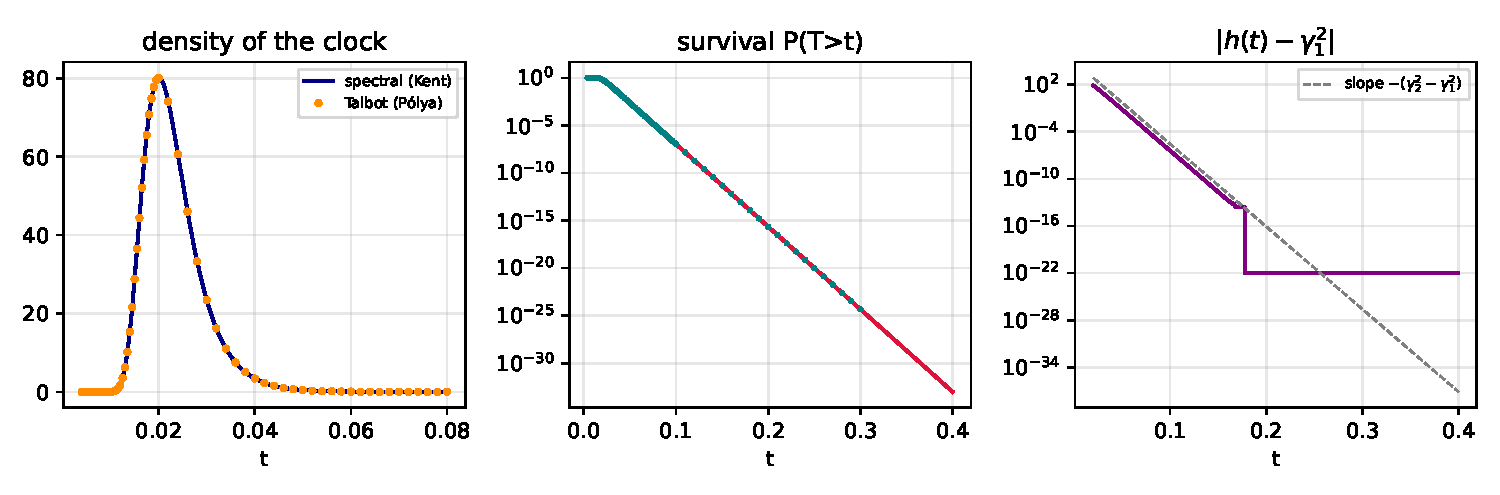
\includegraphics[width=\textwidth]{fig/clocklaw.pdf}
\caption{The law of the clock variable computed from the P\'olya density by Talbot inversion (points) and by the spectral expansion with P\'olya residues (lines): density, survival function, and the distance of the hazard from $\gamma_1^2$, whose logarithm has slope $-(\gamma_2^2-\gamma_1^2)$ (dashed). Beyond $t\approx0.17$ the last curve reflects the double precision of the plotting script, not the hazard.}
\label{fig:clocklaw}
\end{figure}

\subsection{The cost of the zeros in time and in samples}\label{sec:ch18:reach}

The time domain sees the higher atoms only through exponentially subdominant terms. We fit sums of $p$ exponentials to $P(T>t)$ by Prony's method, from $40$ values at $t=0.03,0.032,\dots,0.108$ carrying relative noise from $10^{-16}$ down to $10^{-45}$ (Table~\ref{tab:prony}). With $p=4$ terms the first atom is correct to all nine digits shown, the second to six, the third to four and the fourth to two per cent, and the results do not improve as the noise falls. The error comes from the neglected terms, whose relative size on a window starting at $t_0$ is $e^{-(\gamma_{p+1}^2-\gamma_1^2)t_0}$ up to a factor set by the residues. Resolving the $k$th atom therefore needs data accurate to about $(\gamma_k^2-\gamma_1^2)t_0/\log10$ digits, a number that grows without bound in $k$: a hazard rate method reaches the first atom, and every further atom costs digits.

\begin{table}[t]
\centering\small
\begin{tabular}{rllll}
\toprule
terms & $\gamma_1^2$ & $\gamma_2^2$ & $\gamma_3^2$ & $\gamma_4^2$\\
\midrule
2 & 199.86679 & 427.28 & & \\
3 & 199.79031 & 442.129 & 618.93 & \\
4 & 199.790455 & 441.9255 & 625.63 & 907.24\\
\midrule
true & 199.7904548 & 441.9261506 & 625.5429969 & 925.6730873\\
\bottomrule
\end{tabular}
\caption{Prony extraction of the atoms from $P(T>t)$ on $t\in[0.03,0.108]$. Identical results for relative noise $10^{-16}$, $10^{-30}$ and $10^{-45}$: the error is model truncation, not noise.}
\label{tab:prony}
\end{table}

Sampling meets the same cancellation in another currency. By the identity $2\xi(s)=\E[(\pi S_2/2)^{s/2}]$ of Section~\ref{ch:clock}, with $S_2=\sum_{k\ge1}\frac2{\pi^2k^2}\Gamma_k$ for independent Gamma$(2,1)$ variables $\Gamma_k$, the variable $Y=\frac12\log(\pi S_2/2)$ satisfies
\[
2\,\Xi(z)=\E\big[e^{Y/2}\cos(zY)\big].
\]
The P\'olya variable is $Y$ tilted by $e^{Y/2}$, and $\Xi(z)$ is the mean of a random variable with finite variance, since $\E e^{Y}=2\xi(1)=1$, so a sample mean estimates it at every $z$. We draw $n=10^6$ copies of $S_2$, truncating the series after $2000$ terms and replacing the remainder, whose variance is about $3\times10^{-12}$, by its mean $4/(2000\pi^2)$, and compare the estimates with $\Xi(z)$ in Table~\ref{tab:ch18:mc}, a check of the identity on the critical line; Table~\ref{bp:tab:bpy} checks it at real $s$ (Section~\ref{bp:sec:mellin}).

\begin{table}[htbp]
\centering\small
\begin{tabular}{rllll}
\toprule
$z$ & Monte Carlo & standard error & $\Xi(z)$ & $n$ with standard error $|\Xi(z)|$\\
\midrule
0 & 0.497061 & $5.4\times10^{-5}$ & 0.497121 & $1.2\times10^{-2}$\\
2 & 0.453136 & $7.3\times10^{-5}$ & 0.453100 & $2.6\times10^{-2}$\\
5 & 0.275888 & $2.4\times10^{-4}$ & 0.275550 & $0.77$\\
8 & 0.103756 & $3.4\times10^{-4}$ & 0.103303 & $11$\\
10 & 0.038401 & $3.5\times10^{-4}$ & 0.037968 & $86$\\
20 & 0.000314 & $3.5\times10^{-4}$ & $-3.67\times10^{-5}$ & $9.3\times10^{7}$\\
30 & 0.000289 & $3.5\times10^{-4}$ & $-1.50\times10^{-8}$ & $5.5\times10^{14}$\\
\bottomrule
\end{tabular}
\caption{Monte Carlo estimates of $\Xi(z)$ from Williams' representation with $10^6$ samples. The last column is the sample size at which the standard error equals $|\Xi(z)|$.}
\label{tab:ch18:mc}
\end{table}

The standard error settles at $3.5\times10^{-4}$, the standard deviation of $e^{Y/2}\cos(zY)/2$ over $\sqrt n$, while $|\Xi(z)|$ decays like $e^{-\pi z/4}$. The sample size needed to resolve the sign of $\Xi$ therefore grows like $e^{\pi z/2}$: about $10^8$ at $z=20$ and $10^{15}$ at $z=30$. Even the first sign change, at $z=14.13$, needs about $10^{6}$ samples: between the first two zeros $|\Xi|$ is at most $8.0\times10^{-4}$ (at $z=15.59$), and resolving it at two standard errors takes about $8\times10^5$ samples. Figure~\ref{fig:ch18:mc} shows where $|\Xi|$ falls below the standard error. The P\'olya route pays for the same cancellation in digits of working precision and Monte Carlo pays for it in samples, and precision is exponentially cheaper. Sampling is the right tool for the law of the P\'olya variable itself, for its moments and for the Bayesian inverse problems of \cite[Section 19.2]{P26}, and the wrong tool for the zeros. Devroye's exact samplers for theta type laws \cite{Devroye86} make sampling efficient, but the sample size needed for the zeros still grows like $e^{\pi z/2}$.

\begin{figure}[!ht]
\centering
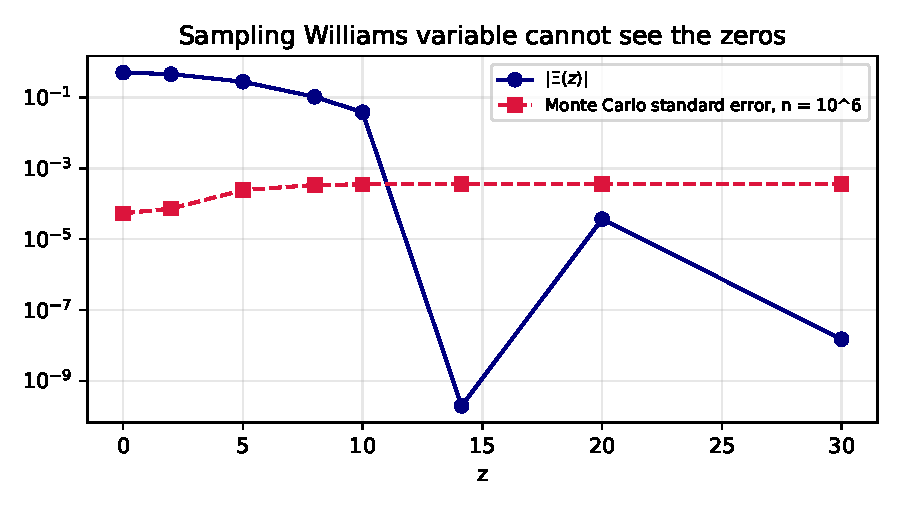
\includegraphics[width=0.72\textwidth]{fig/williams_mc.pdf}
\caption{$|\Xi(z)|$ against the Monte Carlo standard error with $10^6$ samples of Williams' variable $S_2$, at the sampled values of $z$ and at the first zero, joined by straight lines.}
\label{fig:ch18:mc}
\end{figure}

\subsection{Kent approximants with a Weyl tail}\label{sec:ch18:kent}

In the rest of this section we write $w$ for the variable $u$ of the clock, as the tables and figures that follow do. Kent's theorem \cite{Kent80} identifies the first hitting time of a level by a diffusion started at a reflecting or entrance end of its interval with the GGC $\prod_n(1+w/\lambda_n)^{-1}$, where the $\lambda_n$ are the Dirichlet eigenvalues of the interval up to that level; the simplest example is the time a three dimensional Bessel process started at $0$ takes to reach the level one, with $\lambda_n=\pi^2n^2/2$ (Section~\ref{bp:sec:mellin}). Krein's inverse spectral theory \cite{DymMcKean76} builds a string, and so a generalised diffusion, from any increasing sequence $\lambda_n>0$ with $\sum1/\lambda_n<\infty$. The GGCs that arise as such hitting times are therefore exactly those without drift whose Thorin measure consists of unit atoms at distinct points. By Proposition~\ref{prop:rigid} the clock is one of them exactly when RH holds and the zeros are simple, and its diffusion then has Dirichlet spectrum $\{\gamma^2\}$; Section~\ref{ri:sec:kill} reads each $1/\zeta(2k)$, up to an explicit factor, as the probability that this diffusion reaches its level before an independent killing. The shifted clocks above the centre are not hitting times of Kent's kind, but with no hypothesis they are the tilted centre clock run through the inverse local time of a sticky Brownian motion (Section~\ref{ch:bphit}), and Section~\ref{pm:sec:map} places all these processes in one map.

The approximants of the clock that Kent's theorem suggests are the transforms $1/G_N(w)$ of the partial products $G_N(w)=\prod_{k\le N}(1+w/\gamma_k^2)$, each the transform of the hitting time of a finite string with $N$ point masses. They are admissible in the closure criterion of Corollary~\ref{cor:weak:closure}, and they are the approximating sequence, under RH, in the proof of \cite[Proposition 18.10]{P26}; Section~\ref{sec:weak:limits} lists them, with and without the Weyl tail of this section, among the approximants whose positivity is proved independently of $\xi$. They converge slowly. With $\tau_1(N)=\sum_{k>N}\gamma_k^{-2}$, the relative error $G(w)/G_N(w)-1$ of the clock transform lies, under RH, between $w\tau_1(N)$ and $e^{w\tau_1(N)}-1$; it is of order one at $w=100$ for $N=20$ and at $w=1000$ for $N=300$.

We keep the verified zeros as atoms and replace the others by their average density. By the Riemann von Mangoldt formula $N(t)=\vartheta(t)/\pi+1+S(t)$, with the Riemann Siegel theta function $\vartheta$ and the argument function $S(t)=\pi^{-1}\arg\zeta(\frac12+it)$ of Section~\ref{ch:classical}, the zeros above the cutoff $\Theta_N$ have density $\vartheta'(\gamma)/\pi\approx\frac1{2\pi}\log\frac\gamma{2\pi}$, which is positive for $\gamma>6.3$. So
\[
G_N^{\rm W}(w)=\prod_{k\le N}\Big(1+\frac w{\gamma_k^2}\Big)\exp\Big\{\int_{\Theta_N}^\infty\log\Big(1+\frac w{\gamma^2}\Big)\frac{\vartheta'(\gamma)}\pi\,d\gamma\Big\},
\]
with W for Weyl, has reciprocal equal to the Laplace transform of a GGC with $N$ unit atoms and the continuous Thorin density $\vartheta'(\sqrt z)/(2\pi\sqrt z)$ on $z>\Theta_N^2$. That Thorin measure is not a sum of unit atoms, so, unlike $1/G_N$, the approximant is not a hitting time of the kind in Kent's theorem; the closure criterion needs only the GGC property. For $\Theta_N$ we take the Gram point $g_{N-1}$ of Section~\ref{sec:ch5:turing}, where $\vartheta(\Theta_N)/\pi+1=N$. For the values of $N$ used here it lies between $\gamma_N$ and $\gamma_{N+1}$, so $S(\Theta_N)=0$ and the smooth count agrees with the true count at the cutoff, as in Section~\ref{ch:distances}, where $\Theta_{1700}$ is the point $T_*$.

Table~\ref{tab:ch18:kent} compares the two approximants with the clock computed from $\xi$. The Weyl tail improves the approximation by at least two orders of magnitude at every $N$ and $w$ tested. With the first $1700$ zeros ($\gamma_{1700}=2197.26$) its error is $3\times10^{-11}$ at $w=1$ and $3\times10^{-7}$ at $w=10^4$, where the partial product is wrong by a factor of more than a hundred. Figure~\ref{fig:ch18:kent} plots the same data.

\begin{table}[htbp]
\centering\footnotesize
\setlength{\tabcolsep}{4pt}
\begin{tabular}{rllll}
\toprule
$N$ & $w=1$ & $w=100$ & $w=1000$ & $w=10^4$\\
\midrule
1 & $1.8\times10^{-2}$ / $1.3\times10^{-4}$ & $4.8$ / $1.0\times10^{-2}$ & $\gg1$ / $3.3\times10^{-2}$ & $\gg1$ / $4.3\times10^{-2}$\\
20 & $7.2\times10^{-3}$ / $4.3\times10^{-7}$ & $1.04$ / $4.2\times10^{-5}$ & $\gg1$ / $3.7\times10^{-4}$ & $\gg1$ / $1.5\times10^{-3}$\\
79 & $3.6\times10^{-3}$ / $1.5\times10^{-7}$ & $0.43$ / $1.5\times10^{-5}$ & $34$ / $1.5\times10^{-4}$ & $\gg1$ / $1.2\times10^{-3}$\\
300 & $1.6\times10^{-3}$ / $7.4\times10^{-9}$ & $0.17$ / $7.4\times10^{-7}$ & $3.95$ / $7.4\times10^{-6}$ & $\gg1$ / $7.2\times10^{-5}$\\
1700 & $5.0\times10^{-4}$ / $2.9\times10^{-11}$ & $0.051$ / $2.9\times10^{-9}$ & $0.64$ / $2.9\times10^{-8}$ & $142$ / $2.9\times10^{-7}$\\
\bottomrule
\end{tabular}
\caption{Relative error of the clock transform: partial product over $N$ zeros, $|G/G_N-1|$, and with the Weyl tail, $|G_N^{\rm W}/G-1|$. The two measures of error agree to first order, and $\gg1$ marks an error above $10^3$. The partial product values agree with \cite[Section 18.2.1]{P26} where both are given.}
\label{tab:ch18:kent}
\end{table}

\begin{figure}[htbp]
\centering
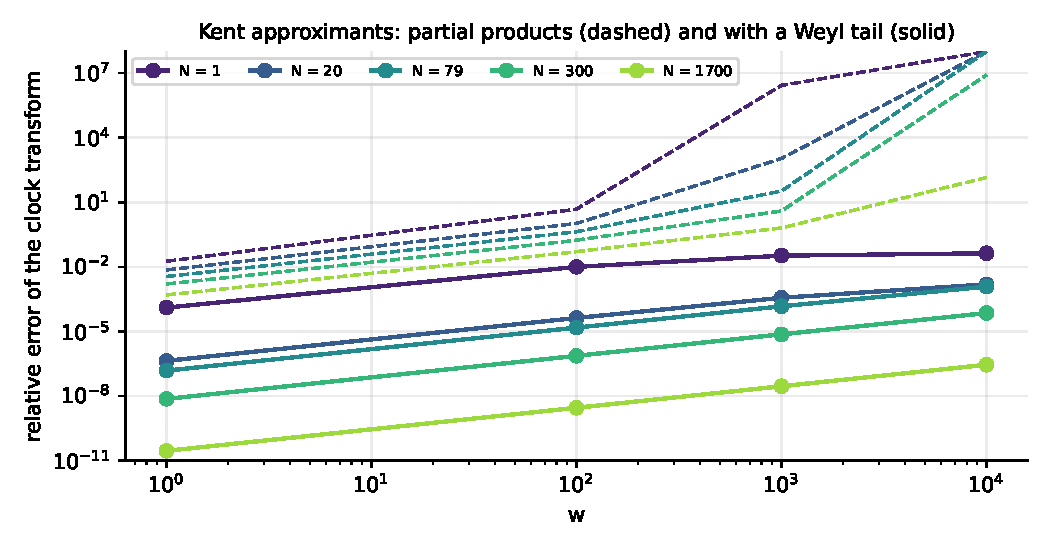
\includegraphics[width=0.8\textwidth]{fig/kenttail.pdf}
\caption{Relative error of Kent approximants to the clock transform, without (dashed) and with (solid) the Weyl tail.}
\label{fig:ch18:kent}
\end{figure}

At the four points $w=1,100,1000,10^4$ the table exhibits an explicit positive Thorin measure whose Thorin transform $\int\log(1+w/z)\,U(dz)$ matches $\log G(w)$ to within $3\times10^{-7}$. This is a finite instance of the weak Thorin condition of \cite[Section 18.2.3]{P26}, which asks for such a measure, to within any $\eta>0$, at every finite set of points, and which is equivalent to RH by the closure criterion of Corollary~\ref{cor:weak:closure}. A finite instance proves nothing: agreement for $w\le10^4$ cannot detect off line zeros above the verified height, which change $\log G$ there by far less than the error. The error of the Weyl tail grows linearly in $w$, and to first order it is a weighted average of $S$ beyond the cutoff,
\[
\log G(w)-\log G_N^{\rm W}(w)\approx w\big(\tau_1(N)-\tau_1^{\rm W}(N)\big)=2w\int_{\Theta_N}^\infty\frac{S(\gamma)}{\gamma^3}\,d\gamma,
\]
where $\tau_1^{\rm W}(N)=\int_{\Theta_N}^\infty\gamma^{-2}\vartheta'(\gamma)\pi^{-1}d\gamma$ is the Weyl estimate of $\tau_1(N)$ and the identity is an integration by parts that uses $S(\Theta_N)=0$. No tail built on the smooth count can follow $S$ without the zeros. The Taylor coefficients of $\xi$ at the centre carry more information, and Section~\ref{sec:ch18:moments} uses them.

\subsection{Moment matching and the error at large $w$}\label{sec:ch18:moments}

The error of the Weyl tail comes from the first order term of $\log(1+w/\gamma^2)=w/\gamma^2-w^2/(2\gamma^4)+\cdots$. For $w$ small compared with $\Theta_N^2$ the error of $\log G_N^{\rm W}$ is approximately $w$ times $\tau_1(N)-\tau_1^{\rm W}(N)$, and the second order term is $-w^2/2$ times the corresponding difference for $\tau_2(N)=\sum_{k>N}\gamma_k^{-4}$. Both true tail sums are available without any zero beyond $\gamma_N$, because the power sums $p_m=\sum_ka_k^{-m}$, with $a_k=-(\rho_k-\frac12)^2$ as in Section~\ref{ch:clock} and equal to $\sum_{\gamma>0}\gamma^{-2m}$ under RH, are Taylor coefficients of $\xi$ at the centre: if $\xi(\frac12+s)/\xi(\frac12)=1+c_2s^2+c_4s^4+\cdots$, then
\begin{gather*}
p_1=\sum_ka_k^{-1}=c_2=0.0231049931154189707889,\\
p_2=\sum_ka_k^{-2}=c_2^2-2c_4=0.0000371725992852696862,
\end{gather*}
and $\tau_m(N)=p_m-\sum_{k\le N}\gamma_k^{-2m}$. Here $p_1=\E T$ and $p_2=\operatorname{Var}T$ (Section~\ref{ch:clock}). We therefore replace the Weyl density $\vartheta'(\gamma)/\pi$ on $[\Theta_N,\infty)$ by $\lambda\,\vartheta'(\gamma)/\pi$ on $[\Theta_N',\infty)$, and choose the two parameters $\lambda$ and $\Theta_N'$ so that the tail reproduces $\tau_1(N)$ and $\tau_2(N)$ exactly. The tail density remains positive, so the approximant is still a GGC. The adjustments are small: for $N=79$ the cutoff moves from $199.649$ to $199.675$ and $\lambda=1.000059$, and for $N=1700$ it moves from $2197.87959$ to $2197.87923$ and $\lambda=0.99999992$.

\begin{table}[htbp]
\centering\footnotesize
\setlength{\tabcolsep}{4pt}
\begin{tabular}{rlllllll}
\toprule
$N$ & tail & $w=1$ & $w=10^2$ & $w=10^4$ & $w=10^5$ & $w=10^6$ & $w=10^7$\\
\midrule
79 & Weyl & $1.5\times10^{-7}$ & $1.5\times10^{-5}$ & $1.2\times10^{-3}$ & $4.3\times10^{-3}$ & $5.8\times10^{-3}$ & $6.0\times10^{-3}$\\
 & matched & $2.6\times10^{-17}$ & $2.6\times10^{-11}$ & $1.8\times10^{-5}$ & $3.1\times10^{-3}$ & $6.1\times10^{-2}$ & $0.47$\\
\addlinespace
300 & Weyl & $7.4\times10^{-9}$ & $7.4\times10^{-7}$ & $7.2\times10^{-5}$ & $5.5\times10^{-4}$ & $1.7\times10^{-3}$ & $2.1\times10^{-3}$\\
 & matched & $2.3\times10^{-20}$ & $2.3\times10^{-14}$ & $2.2\times10^{-8}$ & $1.5\times10^{-5}$ & $1.8\times10^{-3}$ & $2.8\times10^{-2}$\\
\addlinespace
1700 & Weyl & $2.9\times10^{-11}$ & $2.9\times10^{-9}$ & $2.9\times10^{-7}$ & $2.8\times10^{-6}$ & $2.4\times10^{-5}$ & $9.3\times10^{-5}$\\
 & matched & $3.5\times10^{-23}$ & $1.1\times10^{-17}$ & $7.0\times10^{-13}$ & $3.6\times10^{-10}$ & $2.5\times10^{-7}$ & $5.0\times10^{-5}$\\
\bottomrule
\end{tabular}
\caption{Relative error $|G_{\rm a}/G-1|$ of the approximant $G_{\rm a}$ of $G$ with the Weyl tail and with the moment matched tail. The cutoffs are $\Theta_N^2=3.99\times10^4$, $2.95\times10^5$ and $4.83\times10^6$ for $N=79$, $300$ and $1700$.}
\label{tab:ch18:kent2}
\end{table}

\begin{figure}[htbp]
\centering
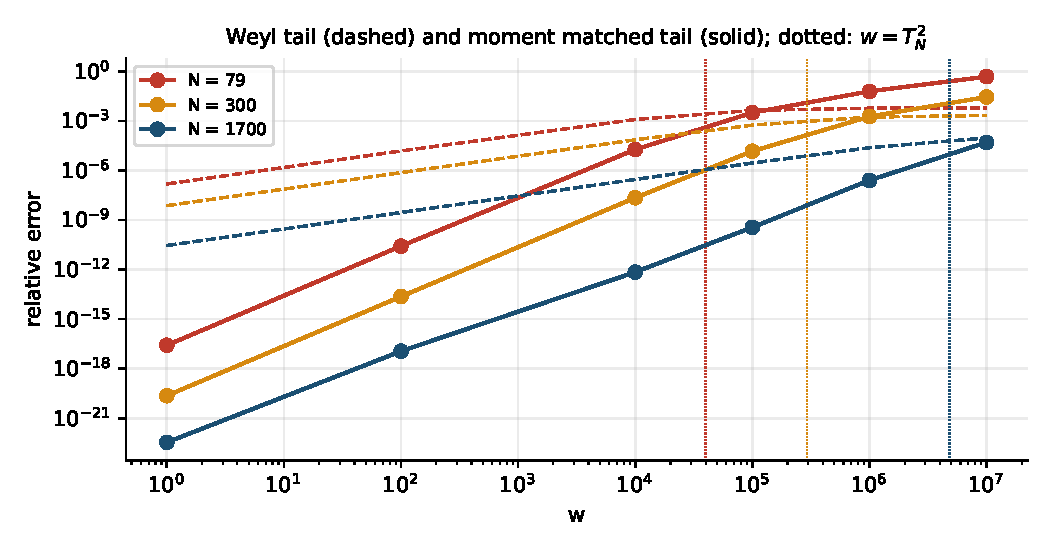
\includegraphics[width=0.8\textwidth]{fig/kenttail2.pdf}
\caption{The Kent approximants at large $w$, with the dotted lines at $w=\Theta_N^2$ (labelled $T_N^2$ in the plot). Moment matching gains ten to twelve digits at $w=1$ and about two as $w$ approaches $\Theta_N^2$. Beyond $\Theta_N^2$ the Weyl tail levels off at a floor set by $S$, while the error of the matched tail, whose density is rescaled by $\lambda$, grows like $|\lambda-1|\sqrt w\log w$.}
\label{fig:ch18:kent2}
\end{figure}

Table~\ref{tab:ch18:kent2} and Figure~\ref{fig:ch18:kent2} show two regimes. For $w$ below $\Theta_N^2$ moment matching gains ten to twelve digits at $w=1$ and about two as $w$ approaches $\Theta_N^2$: with $1700$ zeros the error at $w=10^4$ falls from $2.9\times10^{-7}$ to $7\times10^{-13}$, and at $w=10^5$ from $2.8\times10^{-6}$ to $3.6\times10^{-10}$. Well beyond $\Theta_N^2$ the gain disappears, and at $w=10^7$ with $N=79$ the matched tail is worse than the plain Weyl tail. The cause is the rescaling of the whole tail. For $w\gg\Theta_N^2$ the matched tail differs from the Weyl tail mainly by $(\lambda-1)\int_{\Theta_N'}^\infty\log(1+w/\gamma^2)\,\vartheta'(\gamma)\pi^{-1}d\gamma$, which grows like $(\lambda-1)\frac{\sqrt w}2\log\frac{\sqrt w}{2\pi}$, while the error of the Weyl tail tends to a constant.

That constant is a weighted average of $S$ beyond the cutoff. Under RH, since $S(\Theta_N)=0$ and no ordinate lies in $(\gamma_N,\Theta_N]$, the true tail sum minus its Weyl estimate is a Stieltjes integral against $S$, and an integration by parts gives
\begin{align*}
\log G_N^{\rm W}(w)-\log G(w)&=-\int_{\Theta_N}^\infty\log\Big(1+\frac w{\gamma^2}\Big)\,dS(\gamma)=-\int_{\Theta_N}^\infty\frac{2w\,S(\gamma)}{\gamma(\gamma^2+w)}\,d\gamma\\
&\longrightarrow\;-2\int_{\Theta_N}^\infty\frac{S(\gamma)}\gamma\,d\gamma\qquad(w\to\infty).
\end{align*}
The limit is $-\ell_N$, with $\ell_N=2\int_{\Theta_N}^\infty S(\gamma)\gamma^{-1}\,d\gamma$ as in Exercise~\ref{ex:ch18:floor}. It is finite because $\int_0^tS(u)\,du=O(\log t)$ (Littlewood; Section~\ref{sec:ch5:turing}), and in general it is not zero. The measured errors of the Weyl tail level off at about $6\times10^{-3}$ for $N=79$ and $2\times10^{-3}$ for $N=300$; for $N=1700$ the error is still rising at $w=10^7$, where it is $9.3\times10^{-5}$, so its level is not yet reached.

The constant is not an obstruction of principle. It depends only on $\gamma_1,\dots,\gamma_N$ and on $\xi$ along the real axis, and Stirling's formula gives $\ell_N$ in closed form (Exercise~\ref{ex:ch18:floor}). It is also a floor only for the Weyl density. Adding to $\vartheta'/\pi$ a continuous $\omega$ with compact support in $(\Theta_N,\infty)$ and $\int\omega=0$ changes the limit by $-2\int\omega(\gamma)\log\gamma\,d\gamma$, and two wide bumps of opposite sign placed far apart give this any value while the density stays positive, so a suitable positive tail removes the constant.

Of the two tails computed here, the matched tail is the better one for $w$ up to about $\Theta_N^2$ and the plain Weyl tail beyond. With them the clock is within a small computed distance of an explicit GGC at every scale computed, and at large $w$ that distance is a weighted integral of $S$ beyond the cutoff, the quantity whose integrals Turing's method bounds (Section~\ref{ch:turing}).

\section{Brownian boundaries and Williams' structure}\label{ch:boundaries}

Under RH with simple zeros, Kent's theorem makes the clock variable $T$ the hitting time of a level by a diffusion, but it describes that diffusion only through its spectrum, the set $\{\gamma^2\}$ that is to be found (Section~\ref{sec:ch18:kent}). We look instead for a representation by Brownian motion itself. Unconditionally, $T$ is not a Brownian first passage time to an independent random level for any constant drift (Section~\ref{sec:ch19:nogo}). Across a curved boundary it is one: such a boundary exists by a theorem of Ekstr\"om and Janson, and we compute it (Section~\ref{sec:hitting}). Williams' representation of the P\'olya kernel through Bessel hitting times explains the tilted contour of Section~\ref{sec:newcomp}, but it transfers no positivity to the clock (Section~\ref{sec:ch19:williams}).

\subsection{The clock is not a first passage time to a random level}\label{sec:ch19:nogo}

The first passage time of Brownian motion with drift $c\ge0$ to a level $a>0$ has the inverse Gaussian law, with transform $\exp\{a(c-\sqrt{c^2+2u})\}$. Mixing over an independent random level with law $F$ gives the transforms $\int\exp\{a(c-\sqrt{c^2+2u})\}F(da)$, a class of first passage laws.

\begin{proposition}\label{prop:nogo}
For no drift $c\ge0$ and no probability law $F$ on $(0,\infty)$ is the clock variable $T$ equal in law to the first passage time of Brownian motion with drift $c$ to an independent level $A\sim F$.
\end{proposition}

\begin{proof}
On the parabola $u=\tfrac12(-q^2+2icq)$, $q\in\mathbb R$, we have $c^2+2u=(c+iq)^2$, so $\re\sqrt{c^2+2u}=c$ and every mixture transform has modulus at most one there. Suppose that $T$ had such a law, so that the clock transform $1/G(u)=\E e^{-uT}$ and the mixture transform agree for $u\ge0$. The mixture transform is analytic and bounded by one on the region $D=\{u:\re\sqrt{c^2+2u}>c\}$, and continuous up to its boundary, which is the parabola. The region $D$ is the image of the half plane $\re v>c$ under $v\mapsto(v^2-c^2)/2$, so it is connected, and it contains the right half plane. By the identity theorem $1/G$ coincides with the mixture transform on $D$, so it has no pole in $D$ and is bounded by one there, and by continuity $|1/G|\le1$ on the parabola away from the zeros of $\xi(\tfrac12+\sqrt u)$. For the clock, however, $\sqrt u=(c+iq)/\sqrt2+O(1/q)$ as $q\to\infty$ (for $c=0$ the parabola is the negative axis, approached from above, and $\sqrt u=i|q|/\sqrt2$), so $|\xi(\tfrac12+\sqrt u)|$ decays like $\exp(-\pi|q|/(4\sqrt2))$ times a power, by Stirling's formula and the polynomial growth of $\zeta$ in vertical strips. Hence $|\xi(\tfrac12)/\xi(\tfrac12+\sqrt u)|$ grows exponentially along the parabola, and the transforms cannot agree.
\end{proof}

The proof covers the nonincreasing lines $a-ct$, $c\ge0$; an increasing line, with $c<0$, gives a passage time that is infinite with probability $1-\E e^{2cA}>0$, which the clock is not. Expanding $G(u)=1+m_1u+m_2u^2+\cdots$ with $m_1=\E T$ and $m_1^2-2m_2=\mathrm{Var}\,T$ gives $|G(u)|^2=1-q^2(m_1-c^2\,\mathrm{Var}\,T)+O(q^3)$ on the parabola, so the clock transform already exceeds one at small $q$ whenever
\[
c<c_*=\sqrt{\E T/\mathrm{Var}\,T}=\sqrt{0.0231050/3.71726\times10^{-5}}=24.93 .
\]


\subsection{A curved Brownian boundary for the clock}\label{sec:hitting}

Finding a boundary whose first passage time has a prescribed law is the inverse first passage problem \cite[Theorem 1]{CCCS11}. By the theorems of Ekstr\"om and Janson \cite[Theorems 2.3, 8.2 and 9.2]{EkstromJanson16}, stated in full in Section~\ref{bp:sec:rs1}, the problem has a solution for the clock, which we call the exact boundary. Since the density of the clock is continuous and positive on $(0,\infty)$ (Exercise~\ref{ex:ch19:density}), the same theorems make the exact boundary continuous on $(0,\infty)$ and the unique continuous solution $b$ with $\liminf_{t\downarrow0}b(t)\ge0$ of the Volterra integral equation \eqref{eq:ch19:volterra} of the first passage density. We call the solution of the discretised Volterra equation the Volterra boundary.

\subsubsection{The Roberts Shortland tangent boundary}\label{sec:ch19:tangent}

Roberts and Shortland \cite{RS95} approximate the hazard of a Brownian first passage across a smooth boundary $b$ by the hazard of the tangent line at the current time, for which the Bachelier L\'evy formula is exact:
\begin{gather*}
h_{\rm tan}(t)=\frac{\alpha(2\pi t^3)^{-1/2}\exp\{-(\alpha+\beta t)^2/2t\}}{\mathcal N\big((\alpha+\beta t)/\sqrt t\big)-e^{-2\alpha\beta}\mathcal N\big((\beta t-\alpha)/\sqrt t\big)},\\
\beta=b'(t),\ \alpha=b(t)-tb'(t),
\end{gather*}
where $\mathcal N$ is the standard normal distribution function; we write $\overline{\mathcal N}=1-\mathcal N$ for its tail. We use the formula in reverse. Setting $h_{\rm tan}(t)=h(t)$, the computed hazard of the clock, defines an ordinary differential equation for $b$, which we integrate by the fourth order Runge Kutta method with step $10^{-4}$ from $t_0=0.011$. The starting value $b(t_0)=0.4023$ is the constant level with the crossing mass of the clock, $2\overline{\mathcal N}(b(t_0)/\sqrt{t_0})=P(T\le t_0)=1.25\times10^{-4}$.

The boundary falls steeply at first, with slope $-87.5$ at $t_0$, and then becomes asymptotically linear with slope tending to $-\sqrt2\,\gamma_1=-19.99$, since an inverse Gaussian hazard tends to $\beta^2/2$.

\subsubsection{The boundary from the Volterra equation}\label{sec:ch19:zones}

The Volterra equation of the first passage density determines the exact boundary (Section~\ref{sec:hitting} and \cite[Theorems 9.1 and 9.2]{EkstromJanson16}), and solving its discretisation for the clock needs three zones: small times, the bulk and the right tail.

For a continuous boundary $b$ with $b(0+)>0$, the first passage density $f$ of Brownian motion started at $0$ satisfies the Volterra equation of the first kind \cite{Peskir02}
\begin{equation}\label{eq:ch19:volterra}
\begin{aligned}
P\big(B_t\ge b(t)\big)&=\int_0^tf(s)\,P\big(B_t\ge b(t)\mid B_s=b(s)\big)\,ds,\\
\text{that is}\quad\overline{\mathcal N}\Big(\frac{b(t)}{\sqrt t}\Big)&=\int_0^tf(s)\,\overline{\mathcal N}\Big(\frac{b(t)-b(s)}{\sqrt{t-s}}\Big)ds,
\end{aligned}
\end{equation}
with $\overline{\mathcal N}$ the standard normal tail. In the inverse problem we know $f$, the density of the clock computed in Section~\ref{ch:clocklaw}, and solve for $b$ one time step at a time, since once $b$ is known at the earlier grid points the discretised equation at time $t$ is a single scalar equation for $b(t)$. We discretise with $2900$ steps on $[0.009,0.3]$, midpoint quadrature in $s$, and a scalar root search at each step.

Before $t_0=0.009$ the clock has crossed with probability only $P(T\le t_0)=1.42\times10^{-7}$. Its density is super flat: it vanishes to all orders at $t=0$, like $\exp(-(1+o(1))\log^2(1/t)/(16t))$, as the growth $\log G(u)\sim\frac14\sqrt u\log u$ at infinity dictates; de Bruijn's exponential Tauberian theorem \cite[Theorem 4.12.9]{BGT87} gives this rate for $P(T\le t)$, and the density has the same rate because the clock is unimodal (Corollary~\ref{sb:cor:unimodal}). So the exact boundary is unbounded as $t\downarrow0$: a path above $b(t)$ at time $t$ has crossed by then, so $\overline{\mathcal N}(b(t)/\sqrt t)\le P(T\le t)$, which forces $b(t)\ge(1+o(1))\log(1/t)/(2\sqrt2)$. In this first zone we replace the exact boundary by a constant level, fixed by the reflection principle, $2\overline{\mathcal N}(b/\sqrt{t_0})=P(T\le t_0)$, which gives $b(t_0)=0.4992$. The Volterra boundary then falls from $0.4992$ to $0.3908$ at $t=0.011$. The tangent boundary starts there at $0.4023$, the constant level with the same crossing mass by time $0.011$; a boundary that decreases on $[0,0.011]$ with that crossing mass must end below this level, so the gap is no defect of the tangent approximation.

In the bulk, between $t=0.011$ and $t=0.05$, the Volterra and tangent boundaries agree closely: $0.0721$ against $0.0710$ at $t=0.02$, and $-0.5894$ against $-0.5954$ at $t=0.05$. Here there is no cancellation: both sides of \eqref{eq:ch19:volterra} are of order one.

In the right tail the equation cancels. Solved in the form \eqref{eq:ch19:volterra}, the computation fails at $t=0.0937$, where the clock has survival probability $3.8\times10^{-7}$: both sides of the equation are within that amount of $P(T\le t)\approx1$. In general the absolute error of the quadrature must stay below $P(T>t)$, which is $5\times10^{-25}$ at $t=0.3$, beyond double precision. The cure is to subtract the equation from $P(T\le t)=\int_0^tf$, which gives the complementary form
\[
\mathcal N\Big(\frac{b(t)}{\sqrt t}\Big)-P(T>t)=\int_0^tf(s)\,\mathcal N\Big(\frac{b(t)-b(s)}{\sqrt{t-s}}\Big)ds,
\]
in which every term is small and computed without cancellation, provided the survival function itself is known to relative accuracy. The spectral expansion of Section~\ref{ch:clocklaw} supplies it to full working precision, even where $P(T>t)$ is of order $10^{-25}$. With the switch made where $P(T>t)$ falls below one half, the solution runs smoothly to $t=0.3$.

In this zone the boundary is nearly linear with slope $\beta=-\sqrt2\gamma_1=-19.99$. A linear boundary does not suffice. Its crossing time has survival function of order $t^{-3/2}e^{-\beta^2t/2}$, while that of the clock is asymptotic to a multiple of $e^{-\gamma_1^2t}$. The power $t^{-3/2}$ is removed by a logarithmic correction: for $b(t)=\beta t+a+\kappa\log t$ the Gaussian factor $e^{-b(t)^2/2t}$ acquires $t^{-\kappa\beta}$, and $\kappa\beta=-\frac32$ cancels the power. So the right tail boundary is
\[
b(t)\approx\beta t+a+\frac{3}{2|\beta|}\log t,\qquad \beta=-\sqrt2\,\gamma_1,\qquad \frac3{2|\beta|}=0.0750 .
\]
Fitting $a$ on $[0.15,0.3]$ gives $a=0.578$ with largest residual $0.0095$. The slope of the Volterra boundary over $[0.2,0.3]$ is $-19.77$. It lies between the slope $-19.99$ without the logarithm and the slope $-19.99+0.075/0.25=-19.69$ of the asymptote at $t=0.25$.

We simulate $n=2\times10^5$ Brownian paths against both boundaries with step $2\times10^{-5}$ and a Brownian bridge crossing correction; sampling noise alone gives a Kolmogorov distance of about $0.87/\sqrt n\approx0.002$. For the Volterra boundary the Kolmogorov distance to the law of the clock is $0.0020$, at the level of the Monte Carlo noise, and the mean crossing time is $0.023085$ against $\E T=0.0231050$. For the tangent boundary the distance is $0.0059$ and the mean $0.023021$ (Figure~\ref{fig:ch19:zones}). The right tail itself cannot be checked by plain simulation, since only about one path in ten million survives past $t=0.1$.

Wald's identities constrain the exact boundary as a whole. Since $\E T$ is finite, the first passage time $H$ across it satisfies $\E B_H=0$ and $\E B_H^2=\E H$, and since $B_H=b(H)$ and $H$ has the law of the clock, $\int_0^\infty b(t)f(t)\,dt=0$ and $\int_0^\infty b(t)^2f(t)\,dt=\E T$.

\begin{figure}[htbp]
\centering
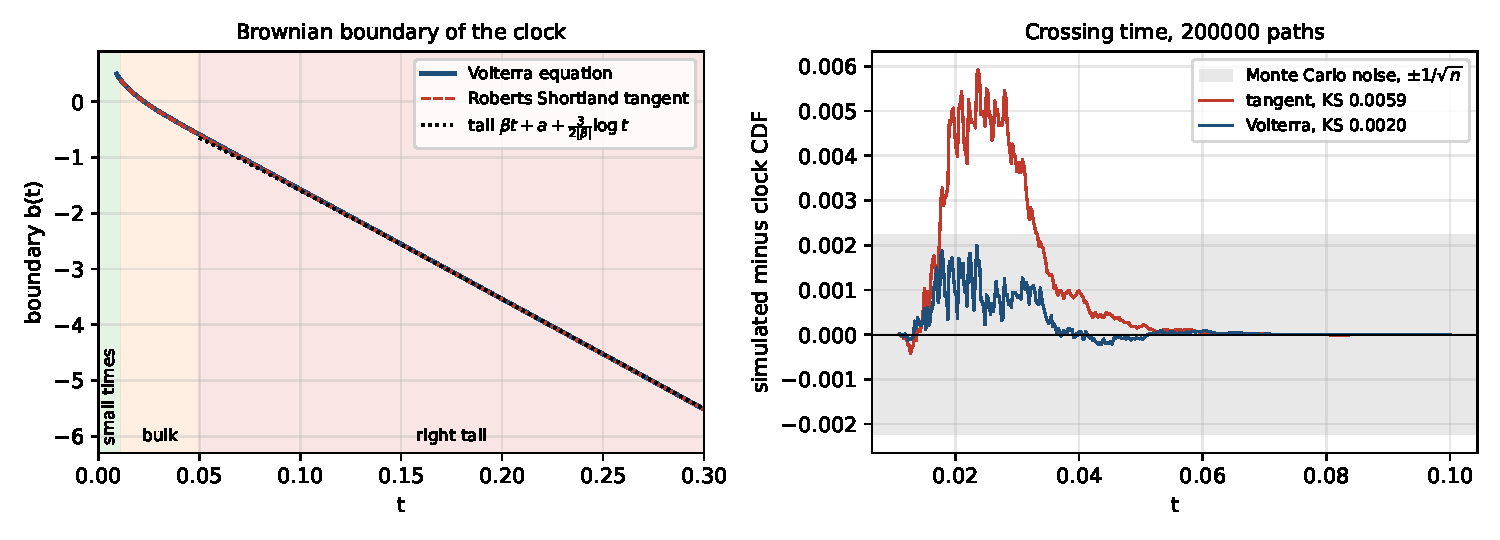
\includegraphics[width=\textwidth]{fig/threezones.pdf}
\caption{Left: the Brownian boundary of the clock computed from the Volterra equation, the Roberts Shortland tangent boundary, and the right tail asymptote with its logarithmic correction, over the three zones. Right: the simulated distribution function of the crossing time minus that of the clock, for both boundaries; the grey band is $\pm1/\sqrt n$, twice the largest standard error of a simulated distribution function.}
\label{fig:ch19:zones}
\end{figure}

\subsection{Williams' Gamma(2) structure: the tilt, a benchmark and its limits}\label{sec:ch19:williams}

Williams \cite{Williams90} and Biane, Pitman and Yor \cite{BPY01} showed that the variable $S_2=\sum_{n\ge1}\frac2{\pi^2n^2}\Gamma_n$ of Section~\ref{sec:ch18:reach} is a sum of two independent hitting times of level one by the three dimensional Bessel process started at $0$, and that $2\xi(s)=\E[(\pi S_2/2)^{s/2}]$, so that the P\'olya variable is $Y=\frac12\log(\pi S_2/2)$ tilted by $e^{Y/2}=(\pi S_2/2)^{1/4}$ (Section~\ref{ch:clock}; \cite[Section 16.2.1]{P26}). The Thorin measure of $S_2$ has atoms of mass two at the points $\pi^2n^2/2$, the Gamma(2) shape of a sum of two copies.

First, the tilt. Write $y$ for the variable of the P\'olya kernel, so that the value $y$ of $Y$ corresponds to the value $e^{2y}$ of $\pi S_2/2$. Moving the line of integration from the real axis to the line $\im y=\eta$, as in Proposition~\ref{prop:tilt}, rotates $e^{2y}$ by the angle $2\eta$ into the complex plane. The density of $S_2$, a theta series in its argument, continues analytically to the right half plane, and the boundary of that half plane, the natural boundary of the theta function \cite[Chapter 11, Section 1.4, and Chapter 5, Section 3.2]{Remmert98}, is reached exactly at $\eta=\pi/4$. So the admissible tilts of Proposition~\ref{prop:tilt} are the rotations of Williams' variable within the half plane of analyticity of its density, and the saving $e^{-\eta\theta}$ is the factor gained by that rotation.

Second, a benchmark. Since $\pi^2S_2/2=\sum_n\Gamma_n/n^2$, the Thorin measure of $\pi^2S_2/2$ is $2\sum_n\delta_{n^2}$, and in the square root variable its Cauchy flow $P_\varepsilon*2\sum_n\delta_n$ is explicit \cite[Section 16.4]{P26}. On this measure the distances of Section~\ref{ch:distances} separate the effects of the method from those of the arithmetic, and they need no separate computation: $\pi^2S_2/2$ is the sum of two independent copies of the sinh clock of Section~\ref{sec:ch3:bench}, so its distances follow from the closed forms of that section (Section~\ref{sec:open:calib}).

Third, the limits. Williams' atoms are the Dirichlet eigenvalues $\pi^2n^2/2$ of an interval, and they live on the Laplace side of the kernel. The zeros of $\xi$ live on the Mellin side of the same variable, and they reappear as unit atoms only on the Laplace side of the reciprocal. The Gamma(2) structure therefore gives positivity and an exact sampler \cite{Devroye86} on the kernel side, but it transfers no positivity to the Thorin measure of the clock. In particular it does not give a positive Gamma(2) scale mixture representation of the P\'olya density, a route that \cite[Section 12.6]{P26} excludes.

\section{Keiper Li coefficients from the P\'olya density}\label{ch:li}

The P\'olya density that computes the law of the clock also computes the coefficients of Li's criterion \cite{Li97}, which states that RH holds if and only if
\[
\lambda_n=\sum_\rho\Big[1-\Big(1-\frac1\rho\Big)^n\Big]\ge0\qquad\text{for every }n\ge1,
\]
the sum over the zeros taken in conjugate pairs. Keiper \cite{Keiper92} introduced the coefficients $\lambda_n$ and computed them before Li proved the criterion, and Bombieri and Lagarias \cite{BL99} derived an arithmetic expression for them from the explicit formula and related the criterion to Weil's.

\subsection{Taylor coefficients of \texorpdfstring{$\log\xi$}{log xi} at \texorpdfstring{$s=1$}{s=1}}\label{sec:ch20:compute}

Li \cite{Li97} expresses the coefficients as derivatives at $s=1$,
\[
\lambda_n=\frac1{(n-1)!}\frac{d^n}{ds^n}\Big[s^{n-1}\log\xi(s)\Big]_{s=1}.
\]
With $\log\xi(1+w)=\sum_{k\ge0}a_kw^k$ and $(1+w)^{n-1}=\sum_j\binom{n-1}jw^j$, comparing the coefficients of $w^n$ gives
\begin{equation}\label{eq:ch20:li}
\lambda_n=n\sum_{j=0}^{n-1}\binom{n-1}j\,a_{n-j},
\end{equation}
so the computation reduces to the Taylor coefficients of $\log\xi$ at $s=1$. The zeros nearest to $s=1$ are $\frac12\pm14.1347i$, so $\log\xi(1+w)$ is analytic in the disc $|w|<R$, where $R=|\rho_1-1|=14.1436$.

The sum \eqref{eq:ch20:li} is exact, but its terms can be larger than $\lambda_n$. The Hadamard product $\xi(1+w)=\xi(1)\prod_\rho(1-w/(\rho-1))$ gives $ma_m=-\sum_\rho(\rho-1)^{-m}$ for $m\ge2$, and for large $m$ the two zeros nearest to $s=1$ dominate this sum, so that $|ma_m|$ is at most about $2R^{-m}$. Since $n\binom{n-1}{m-1}=m\binom nm$, the terms of \eqref{eq:ch20:li} are $\binom nm\,ma_m$ with $m=n-j$, and for large $n$ their absolute sum is at most about $2(1+1/R)^n$. Cancellation therefore costs at most about $\log_{10}\big(2(1+1/R)^n/\lambda_n\big)$ digits. This grows like $n\log_{10}(1+1/R)\approx0.03n$ and is about one digit at $n=100$, where $2(1+1/R)^{100}\approx1.9\times10^3$ and $\lambda_{100}=118.6$.

We compute the $a_k$ by the trapezoid rule for the Cauchy integral on the circle $|w|=6$,
\[
a_k\approx\frac1{Nr^k}\sum_{j=0}^{N-1}\log\xi\big(1+re^{2\pi ij/N}\big)e^{-2\pi ijk/N},\qquad r=6,\ N=512,
\]
which converges geometrically. The rule returns $a_k+a_{k+N}r^N+a_{k+2N}r^{2N}+\cdots$, so aliasing changes $a_k$ by a relative amount of about $(r/R)^N\approx10^{-191}$. Rounding errors in the sum are amplified in $a_k$ by about $(R/r)^k$, which is $10^{37}$ at $k=100$ and is absorbed by the working precision.

Each value $\xi(1+w)=\xi(\frac12+(\frac12+w))$ comes from the P\'olya route at $600$ bits; the imaginary part of $\frac12+w$ never exceeds $6$, so the P\'olya sum loses almost nothing to cancellation. The principal branch of the logarithm is the analytic one, because $|\arg\xi(1+w)|<1$ on the circle: in the Hadamard product \eqref{eq:ch2:hadamard} with $s=\frac12+w$, so that $|s|\le6.5$, the factor $1+s^2/\gamma^2$ of the zeros $\frac12\pm i\gamma$ has argument at most $\arcsin(6.5^2/\gamma^2)\le1.01\cdot6.5^2/\gamma^2$, and since $\sum_{\gamma>0}\gamma^{-2}=0.0231$ these arguments add up to less than $0.99$.

The first coefficient has the closed form $\lambda_1=1+\frac{\gamma_E}2-\frac12\log4\pi$, where $\gamma_E$ is Euler's constant. The P\'olya computation gives
\[
\lambda_1=0.02309570896612103381431025,
\]
in agreement with the closed form to all twenty five digits shown. The same number $\lambda_1=\sum_\rho\rho^{-1}=(\xi'/\xi)(1)$ reappears at the basepoint one (Section~\ref{bp:sec:thorin}): the shifted clock $T_1$ there, with Laplace transform $\xi(1)/\xi(1+\sqrt u)=1-\lambda_1\sqrt u+O(u)$ near $u=0$, has a tail of order $x^{-1/2}$, and $\lambda_1/\pi$ is its Thorin density at the origin in the chart $\theta=\sqrt z$. Table~\ref{tab:ch20:li} lists further values with Keiper's asymptotic $\lambda_n\approx\frac n2(\log n-1-\log2\pi+\gamma_E)$ \cite{Keiper92}.

\begin{table}[htbp]
\centering\small
\begin{tabular}{rll}
\toprule
$n$ & $\lambda_n$ (P\'olya) & Keiper asymptotic\\
\midrule
1 & 0.023095708966121033814 & $-1.13$\\
2 & 0.092345735228046670386 & $-1.57$\\
3 & 0.20763892055432480379 & $-1.74$\\
5 & 0.57554271446117745243 & $-1.63$\\
10 & 2.2793393631931577437 & 0.21\\
20 & 8.7692768720932151296 & 7.35\\
50 & 43.531096488374019299 & 41.28\\
100 & 118.60377537679132993 & 117.23\\
\bottomrule
\end{tabular}
\caption{Keiper Li coefficients from the P\'olya density (all digits shown are correct) and Keiper's leading asymptotic, which becomes accurate only for large $n$.}
\label{tab:ch20:li}
\end{table}

\subsection{Li's criterion as positivity of the Thorin functional}\label{sec:ch20:thorin}

Li's criterion is a statement about the Thorin functional $U$ of Section~\ref{ch:arith}, which has a unit atom at $-(\rho-\frac12)^2$ for each pair $\{\rho,1-\rho\}$ of zeros, on the line or off it. For a zero $\rho$ put $q=1-1/\rho$. Then $1-1/(1-\rho)=1/q$, so the pair contributes $2-q^n-q^{-n}$ to $\lambda_n$; and if $a=-(\rho-\frac12)^2$, with the square root chosen so that $\rho-\frac12=i\sqrt a$, then $q=(2\sqrt a+i)/(2\sqrt a-i)$. This proves the following.

\begin{proposition}\label{prop:ch20:thorin}
Without any hypothesis on the zeros,
\[
\lambda_n=\sum_{\{\rho,1-\rho\}}\varphi_n\Big(-\big(\rho-\tfrac12\big)^2\Big)=\langle U,\varphi_n\rangle,
\]
where
\[
\varphi_n(z)=2-\Big(\frac{2\sqrt z+i}{2\sqrt z-i}\Big)^n-\Big(\frac{2\sqrt z-i}{2\sqrt z+i}\Big)^n
\]
is a rational function of $z$, and $\varphi_n(z)=4\sin^2\big(n\arctan\frac1{2\sqrt z}\big)\ge0$ for $z>0$.
\end{proposition}

The two fractions are exchanged when $\sqrt z$ changes sign, so $\varphi_n$ is a rational function of $z$, with a pole of order $n$ at $z=-\frac14$. At infinity $\varphi_n(z)\sim n^2/z$, so the sum converges absolutely.

For $z>0$ the two fractions are conjugate numbers of modulus one. On the critical line, for $\rho=\frac12+i\gamma$ with $\gamma>0$, the number $1-1/\rho=(\rho-1)/\rho$ has modulus one and argument $\phi_\gamma=2\arctan\frac1{2\gamma}$, and the conjugate zero gives $-\phi_\gamma$. Adding the contributions of $\rho$ and $\bar\rho$,
\[
\lambda_n=\sum_{\gamma>0}2\big(1-\cos(n\phi_\gamma)\big)=\sum_{\gamma>0}4\sin^2\Big(n\arctan\frac1{2\gamma}\Big)\qquad\text{under RH}.
\]
Li's criterion thus says that RH holds if and only if $\langle U,\varphi_n\rangle\ge0$ for every $n$, that is, the Thorin functional is nonnegative on the cone spanned by the $\varphi_n$.

The test function $\varphi_n$ is about $n^2/z$ for $\sqrt z\gg n$ and oscillates between $0$ and $4$ for $\sqrt z\lesssim n/\pi$, so $\lambda_n$ weighs the zeros below height of order $n$ at full size and the higher zeros by about $n^2/\gamma^2$ (Figure~\ref{fig:ch20:test}). Every computed $\lambda_n$ is positive, as it must be: every zero below height $3\times10^{12}$ lies on the line \cite{PT21} and contributes a nonnegative term, while a zero at height $\gamma\gg n$ contributes only about $n^2/\gamma^2$ in absolute value, so the zeros above that height cannot change the sign of $\lambda_n$ for $n\le100$.

\begin{figure}[htbp]
\centering
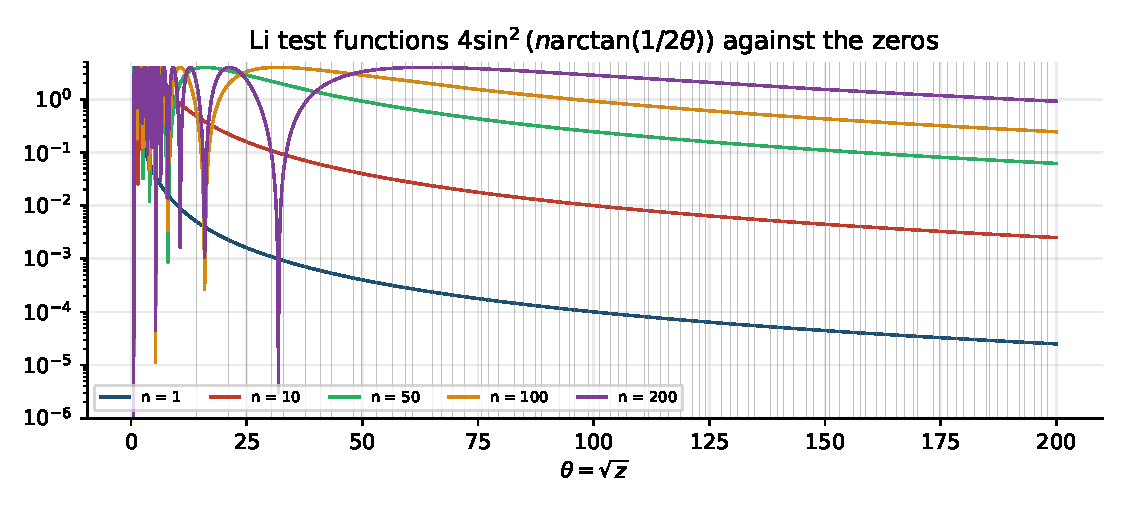
\includegraphics[width=0.9\textwidth]{fig/litest.pdf}
\caption{The Li test functions $4\sin^2(n\arctan\frac1{2\theta})$ for $n=1,10,50,100,200$, in the square root chart $\theta=\sqrt z$, against the zeros below height $200$ (grey vertical lines). Larger $n$ probes higher zeros.}
\label{fig:ch20:test}
\end{figure}

An off line zero makes $|1-1/\rho|\ne1$. For $\rho=\frac12-d+i\gamma$ with $d>0$ one has $|1-1/\rho|^2=1+2d/((\frac12-d)^2+\gamma^2)$, so for large $n$ the term $(1-1/\rho)^n$ grows like $e^{nd/\gamma^2}$, and this is how a failure of RH would eventually make $\lambda_n$ negative (Exercise~\ref{ex:ch20:offline}). Since the exponent is $nd/\gamma^2$, the index at which this happens grows with the height of the zero, so finitely many coefficients, like the finite tests of Section~\ref{ch:finite} (Table~\ref{tab:ch13:see}), cannot exclude an off line zero at great height.

Summing $4\sin^2(n\arctan\frac1{2\gamma})$ over the first $1700$ zeros, computed with \texttt{mpmath} \cite{mpmath} as in Section~\ref{ch:distances}, and adding the tail above $\gamma_{1700}$ with the smooth zero density $\log(\gamma/2\pi)/2\pi$ gives the P\'olya values with relative residuals near $5\times10^{-6}$ for $n\le20$ and $10^{-5}$ at $n=100$. The absolute residual grows like $n^2$ and comes from the cutoff: at $\gamma_{1700}$ the zero count exceeds its smooth part by about one half, so the smooth tail counts about half a term, $\frac12\varphi_n(\gamma_{1700}^2)\approx n^2/(2\gamma_{1700}^2)$, too many.

As a diagnostic the coefficients are poorly localised, so $\lambda_n$ behaves like the heat trace and Bernstein diagnostics of Table~\ref{tab:ch3:diag} and unlike the Thorin density, which is local in the ordinate.

Weil's criterion has the same form as Li's, with the functions of the class $\mathcal T$ of Section~\ref{ch:arith} that are nonnegative on $(0,\infty)$ in place of the $\varphi_n$ (Section~\ref{sec:ch10:positivity}), but the two cones are different. The pole of $\varphi_n$ lies at $-\frac14$, the point at which \eqref{eq:ch14:U} evaluates its test functions, inside the region where $\mathcal T$ requires holomorphy, and $\varphi_n$ decays only like $1/z$. So $\varphi_n$ is not in $\mathcal T$, $\langle U,\varphi_n\rangle$ is defined through the zeros, and the prime side of $\lambda_n$ is the regularised arithmetic formula of Bombieri and Lagarias \cite{BL99}.

\section{The de Bruijn Newman flow from the P\'olya density}\label{ch:dbn}

Li's criterion reads RH from Taylor data at one point, and it tests one fixed Thorin functional against a sequence of test functions (Section~\ref{ch:li}). The de Bruijn Newman flow reads RH from a deformation of the P\'olya kernel, and so deforms the functional instead. Multiplying the kernel by a Gaussian factor turns $\Xi$ into a family of entire functions $H_t$ that evolve by the backward heat equation. RH says that $H_0$ has only real zeros, and the de Bruijn Newman constant $\Lambda$ is defined by the property that $H_t$ has only real zeros exactly when $t\ge\Lambda$. In Thorin terms the flow is a path of clocks that are generalised gamma convolutions for $t\ge\Lambda$ (Theorem~\ref{rz:thm:dbn}), and RH says that the path stays in this class down to $t=0$. The P\'olya route computes $H_t$ at the cost of $\Xi$, since the Gaussian factor only multiplies the node values. We follow two pairs of zeros backward in time to their collisions, the closest pair below height $200$ and Lehmer's pair near height $7005$, and compare the collision times with the isolated pair estimate and with the lower bound of Csordas, Smith and Varga. The Stieltjes moment test of Section~\ref{ch:heat} runs along the flow at the cost of its moments, and a Hankel test of finite order turns out to be a window on the low zeros that registers their collisions one at a time. Biane's description of the free convolution with a semicircle law singles out Laguerre's quantity $-(\log H_0)''$, which predicts the collision times from $H_0$ alone and, with corrections computed along the flow, brackets each of them.

\subsection{The flow, the motion of its zeros and its Thorin form}\label{sec:ch21:flow}

In the normalisation of Rodgers and Tao \cite{RodgersTao}, which Theorem~\ref{rz:thm:dbn} also uses,
\begin{gather*}
H_t(z)=\int_0^\infty e^{tu^2}\Phi_{\rm dBN}(u)\cos(zu)\,du,\\
\Phi_{\rm dBN}(u)=\sum_{n\ge1}\big(2\pi^2n^4e^{9u}-3\pi n^2e^{5u}\big)\exp(-\pi n^2e^{4u}),
\end{gather*}
so that $H_0(z)=\frac18\Xi(z/2)$. If $v=2u$ denotes the variable of \eqref{eq:ch2:Phi}, then $\Phi_{\rm dBN}(u)=\frac12\Phi(v)$ and
\[
8H_t(2\theta)=\int_{\mathbb R}\Phi(v)\,e^{tv^2/4}\cos(\theta v)\,dv,
\]
so the flow multiplies the kernel of \eqref{eq:ch2:Phi} by $e^{tv^2/4}$, and a zero $z$ of $H_t$ corresponds to the ordinate $\theta=z/2$.

De Bruijn showed that $H_t$ has only real zeros for $t\ge\frac12$ and that the property persists forward in time \cite{deBruijn}. Newman showed that there is a constant $\Lambda>-\infty$, at most $\frac12$ by de Bruijn's theorem, such that $H_t$ has only real zeros exactly for $t\ge\Lambda$, and conjectured $\Lambda\ge0$ \cite{Newman1976}, which Rodgers and Tao proved \cite{RodgersTao}. Ki, Kim and Lee sharpened de Bruijn's bound to $\Lambda<\frac12$ \cite{KKL09}, the Polymath project proved $\Lambda\le0.22$ \cite{Polymath}, and Platt and Trudgian improved this to $\Lambda\le0.2$ \cite{PT21}. De Bruijn's bound comes from a theorem about strips: if the zeros of $H_0$ lie in $|\im z|\le\Delta$, then $H_t$ has only real zeros for $t\ge\Delta^2/2$ \cite[Theorem 13]{deBruijn}, and the critical strip gives $\Delta=1$. A zero free half plane $\re s>\alpha$ gives $\Delta=2\alpha-1$, hence $\Lambda\le2(\alpha-\frac12)^2$; for the half plane $\re s>\frac78$ announced in October 2026 (Section~\ref{sec:ch25:open}) this is $\Lambda\le\frac9{32}$, weaker than $0.2$, which a zero free half plane improves only if $\alpha<\frac12+\sqrt{0.1}\approx0.816$. RH is the inequality $\Lambda\le0$, so by the theorem of Rodgers and Tao it is equivalent to $\Lambda=0$: if RH holds, the zeros of $H_t$ are all real from $t=0$ on and at no earlier time.

While the zeros are simple they move according to
\[
\frac{dz_k}{dt}=2\sum_{j\ne k}\frac1{z_k-z_j},
\]
the sum running over all other zeros, positive and negative, with $z_j$ and $-z_j$ taken together. Differentiating $H_t(z_k(t))=0$ in $t$ and using the backward heat equation $\partial_tH_t=-\partial_z^2H_t$ gives $dz_k/dt=\partial_z^2H_t/\partial_zH_t$ at $z_k$, and the Hadamard product of the even function $H_t$ turns this into the display (Exercise~\ref{ex:ch21:motion}). The equation is the gradient flow of unit charges on the line with logarithmic interaction, so forward in time the zeros repel each other, spread and become more regular. Backward in time neighbouring zeros approach each other, and a close pair collides and then leaves the real axis as a conjugate pair. A pair at distance $D$ that is isolated from the other zeros obeys $dD/dt\approx4/D$, so $D^2\approx D_0^2+8t$ with $D_0=D(0)$, and the pair collides at $t\approx-D_0^2/8$. RH is the statement that no two zeros collide at a positive time.

Let $R_t(u)=H_t(0)/H_t(2i\sqrt u)$, where $u$ is the variable of the clock (written $s$ in Chapters~\ref{chap:rzeta} and \ref{chap:rzid}), not the variable of integration in $H_t$, so that $R_0$ is the clock $1/G$. By Theorem~\ref{rz:thm:dbn}, for every $t\ge\Lambda$, and so for every $t\ge0.2$, $R_t$ is the Laplace transform of a GGC with Thorin measure $\sum_k\delta_{(z_k(t)/2)^2}$, where $z_k(t)$ runs over the positive zeros of $H_t$: along the path of clocks the Thorin atoms move with the zeros. The Thorin density at resolution $\varepsilon$ follows the flow in the same way. Put $\xi_t(s)=8H_t\big(-2i(s-\frac12)\big)$, so that $\xi_t(\frac12+i\theta)=8H_t(2\theta)$ and $\xi_0=\xi$, and
\[
\rho_{\varepsilon,t}(\theta)=\pi^{-1}\re(\xi_t'/\xi_t)\big(\tfrac12+\varepsilon+i\theta\big).
\]
Each zero $z$ of $H_t$ gives the zero $\frac12+iz/2$ of $\xi_t$, and for every $t$ the function $\rho_{\varepsilon,t}$ is the sum of the Poisson kernels $P_{\frac12+\varepsilon-\beta}(\theta-\gamma)$ over the zeros $\beta+i\gamma$ of $\xi_t$. For $t\ge\Lambda$ every $\beta$ equals $\frac12$ and $\rho_{\varepsilon,t}$ is the Thorin density of $R_t$ at resolution $\varepsilon$; the P\'olya route computes it by the same multiplication of the node values. As $t$ decreases through a collision, $\rho_{\varepsilon,t}$ shows the off line signature of Section~\ref{ch:offline}: two Poisson peaks merge, and after the collision the pair contributes the kernels $P_{\varepsilon+d(t)}+P_{\varepsilon-d(t)}$ at its ordinate, where $d(t)$, half the imaginary part of the pair in $z$, grows from zero; the second kernel is negative once $d(t)>\varepsilon$. The flow thus produces off line configurations of known geometry, on which the diagnostics of Chapters~\ref{chap:measure} to \ref{chap:heat} can be calibrated; Section~\ref{sec:open:calib} lists this calibration among the open computations.

\subsection{Two collisions computed from the P\'olya kernel}\label{sec:ch21:collisions}

The P\'olya route evaluates $H_t$ at any $t$ by multiplying the node values $\Phi(v_j)$ by $e^{tv_j^2/4}$ and summing. The factor is entire, so the error analysis of Section~\ref{ch:polya} carries over, and for $|t|\le1$ the factor is at most $e^{9/4}$ on the truncation interval $|v|\le3$. Among the $79$ zeros below height $200$ the closest pair is $\gamma_{71}=184.8745$, $\gamma_{72}=185.5988$, at distance $0.7243$ in $\theta$, that is $D_0=1.4486$ in $z$. We follow the pair by the sign changes of $H_t(2\theta)$ at $121$ equally spaced points of $[\gamma_{71}-0.3,\gamma_{72}+0.3]$, computed at $420$ bits, and refine each zero by Newton's method; Table~\ref{tab:ch21:traj} and Figure~\ref{fig:ch21:dbn} show the result.

\begin{table}[htbp]
\centering\small
\begin{tabular}{rll}
\toprule
$t$ & zeros in $\theta=z/2$ & sign changes\\
\midrule
0.2 & 184.676, 185.590 & 2\\
0.1 & 184.771, 185.598 & 2\\
0.0 & 184.874, 185.599 & 2\\
$-0.05$ & 184.931, 185.595 & 2\\
$-0.1$ & 184.992, 185.587 & 2\\
$-0.15$ & 185.059, 185.573 & 2\\
$-0.2$ & 185.136, 185.550 & 2\\
$-0.3$ & none & 0\\
\bottomrule
\end{tabular}
\caption{The closest pair below height $200$ under the de Bruijn Newman flow, located by the sign changes on a grid of step $0.011$ and refined by Newton's method; $t$ is the de Bruijn Newman time.}
\label{tab:ch21:traj}
\end{table}

Bisection on $t$ for the disappearance of the two sign changes gives the collision time
\[
t_*=-0.2880,
\]
with a grid error of at most $6.1\times10^{-5}$. Near a collision the term $4/D$ dominates the motion of the pair, so $D^2\approx8(t-t_*)$ and the gap in $\theta$ is about $\sqrt{2(t-t_*)}$; on a grid of step $h$ the sign changes therefore vanish at a time at most $h^2/2$ above $t_*$. The isolated pair estimate is $-D_0^2/8=-0.262$: the neighbouring zeros, which the estimate ignores, delay the collision. Since nonreal zeros persist backward in time, $H_t$ has nonreal zeros for every $t$ below the collision time, so $\Lambda\ge t_*\approx-0.288$; this numerical lower bound is far weaker than the published bounds, as expected for a pair of ordinary spacing.

\begin{figure}[htbp]
\centering
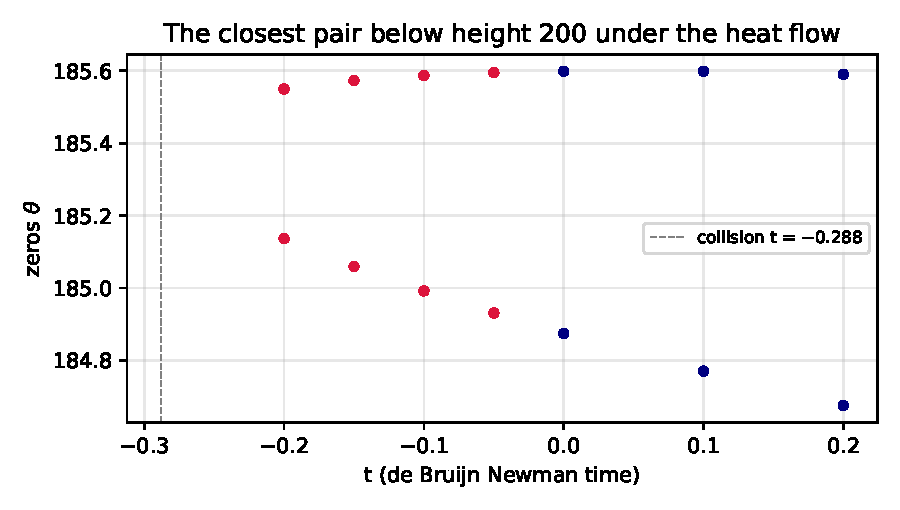
\includegraphics[width=0.7\textwidth]{fig/dbn.pdf}
\caption{Zeros of the closest pair below height $200$ along the de Bruijn Newman flow, refined by Newton's method as in Table~\ref{tab:ch21:traj}, for $t\ge0$ and $t<0$, and the computed collision time (dashed line).}
\label{fig:ch21:dbn}
\end{figure}

Lehmer's pair near height $7005$, $\gamma_{6709}=7005.0629$ and $\gamma_{6710}=7005.1006$ (Section~\ref{sec:ch5:lehmer}), is much closer: $D_0=2\times0.0377=0.0754$, and its isolated pair estimate $-D_0^2/8=-7.1\times10^{-4}$ is about $400$ times closer to zero than the collision time of the pair below height $200$. The tilted P\'olya route evaluates $H_t$ at that height at the same cost as $\Xi$, with the Gaussian factor $e^{tv^2/4}$ included in the exponential at each complex node $v=x+i\eta$. With the parameters of Section~\ref{sec:ch5:lehmer} ($\delta=0.01$, $256$ bits, $13001$ nodes) we track the two sign changes of the pair on a grid of step $0.0025$ in $\theta$ over $[7005.03,7005.13]$. Both sign changes are present at $t=0$ and absent at $t=-0.004$, and twelve bisection steps on this interval give $-7.10\times10^{-4}$, which by the argument above lies above the collision time by at most $0.0025^2/2\approx3\times10^{-6}$. Newton's method for the double zero, $H_t(2\theta)=\partial_\theta H_t(2\theta)=0$ in the unknowns $\theta$ and $t$, started from this value, gives
\[
t_*=-7.11\times10^{-4}
\]
at $\theta=7005.0817$, and Figure~\ref{fig:ch21:lehmerflow} shows the collision. Here the isolated pair estimate is accurate: for a pair this close the neighbours hardly matter, whereas for the ordinary pair below height $200$ they moved the collision from $-0.262$ to $-0.288$. The computation takes about half a minute, and the numerical lower bound $\Lambda\ge t_*$ that it gives is much sharper than the one from the pair below height $200$.

\begin{figure}[htbp]
\centering
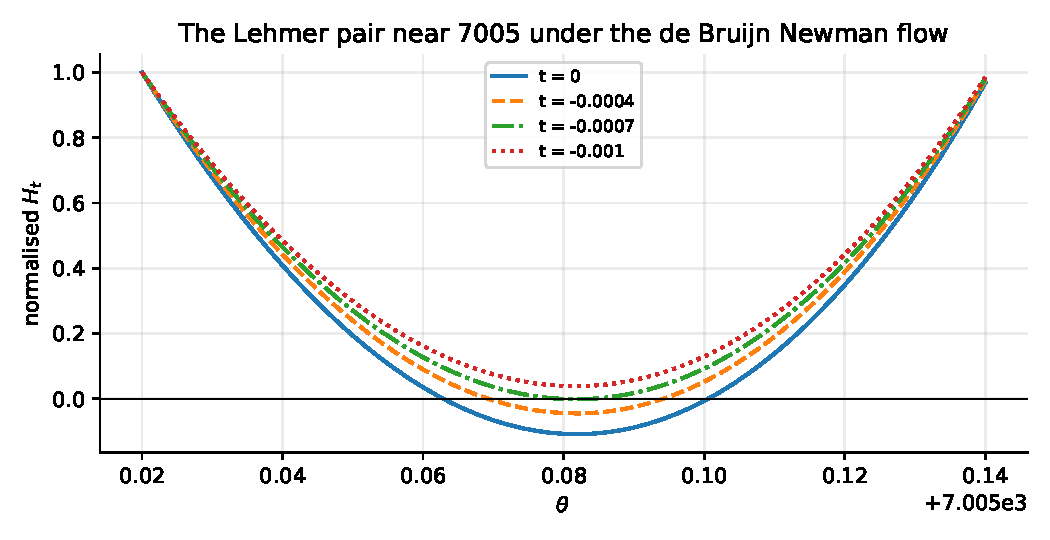
\includegraphics[width=0.8\textwidth]{fig/lehmerflow.pdf}
\caption{The function $\theta\mapsto H_t(2\theta)e^{\pi\theta/4}$ near the Lehmer pair at height $7005$, divided by its maximum absolute value on the window, for four times of the de Bruijn Newman flow, computed with the tilted P\'olya route. At $t=0$ it has two sign changes; at $t=-7\times10^{-4}$, slightly above the collision time $-7.11\times10^{-4}$, they nearly coincide; at $t=-10^{-3}$ the pair has left the real axis.}
\label{fig:ch21:lehmerflow}
\end{figure}

P\'olya's function $K_{i\theta/2}(2\pi)$ behaves differently under the same flow. Down to $t=-60$ none of its real zeros below height $90$ collide, and as $t$ decreases from $0$ to $-0.5$ they rise almost as a rigid block, at speeds within $2\%$ of the mean speed $\pi/8$ that the two functions share, while the zeros of $\Xi$ rise at speeds between $0.004$ and $0.735$; yet by Newman's theorem the de Bruijn Newman constant of P\'olya's function is finite (Section~\ref{sec:biane:flow}).

\subsection{The Hankel test along the flow}\label{sec:ch21:hankel}

The Stieltjes moment test of Section~\ref{ch:heat} (Table~\ref{tab:ch12:jacobi}) needs only the Taylor coefficients of $\Xi$ at the centre, and along the flow these are moments of the reweighted kernel \cite{P26wig}. Putting $\theta=i\sqrt u$ in the formula for $8H_t(2\theta)$ of Section~\ref{sec:ch21:flow} gives
\[
G_t(u)=\frac{H_t(2i\sqrt u)}{H_t(0)}=\sum_{k\ge0}\frac{M_k(t)\,u^k}{(2k)!\,M_0(t)},\qquad M_k(t)=\int_{\mathbb R}v^{2k}e^{tv^2/4}\Phi(v)\,dv,
\]
and $G_0$ is the function $G$ of Section~\ref{ch:heat}. Write $\pm\theta_j(t)$ for the zeros of $\theta\mapsto H_t(2\theta)$, so that $\theta_j(0)=\gamma_j$ while the zeros are on the line. Since $H_t$ is even and entire of order one, $G_t$ has order $\frac12$ and $G_t(u)=\prod_j(1+u/a_j(t))$ with $a_j(t)=\theta_j(t)^2$, so the Newton identities turn the $M_k(t)$ into the moments $m_n(t)=\sum_ja_j(t)^{-n-1}$, exactly as at $t=0$. If every $\theta_j(t)$ is real, the $m_n(t)$ are the moments of the positive measure $\nu_t=\sum_ja_j(t)^{-1}\delta_{1/a_j(t)}$, and every Hankel matrix $\mathcal H_N(t)=[m_{i+j}(t)]_{i,j<N}$ is positive definite. The converse is proved as at $t=0$: if every $\mathcal H_N(t)$ is positive definite, every $a_j(t)$ is real, and it is positive because $H_t$ has no zeros on the imaginary axis: $H_t(iy)=\int_0^\infty e^{tu^2}\Phi_{\rm dBN}(u)\cosh(yu)\,du>0$, the kernel \eqref{eq:ch2:Phi} being strictly positive. So at every time $t$ all the matrices $\mathcal H_N(t)$ are positive definite exactly when $H_t$ has only real zeros, that is, when $t\ge\Lambda$. Each $M_k(t)$ is one sum over the node values of $\Phi$, reweighted by $e^{tv^2/4}$, and the Cholesky factor gives the Jacobi matrix $J_N(t)$, whose eigenvalues return the lowest zeros of $H_t$ as $J_N$ returns the $\gamma_j$ at $t=0$ (Table~\ref{tab:ch21:flowzeros}).

\begin{table}[htbp]
\centering\small
\begin{tabular}{rlllll}
\toprule
$t$ & $\theta_1(t)$ & $\theta_2(t)$ & $\theta_3(t)$ & $\theta_5(t)$ & $\theta_{10}(t)$\\
\midrule
$0.2$ & 14.07681 & 20.94669 & 24.95221 & 32.88801 & 49.72988\\
$0$ & 14.13473 & 21.02204 & 25.01086 & 32.93506 & 49.77383\\
$-0.4$ & 14.25083 & 21.17365 & 25.12774 & 33.02595 & 49.85213\\
$-1.0$ & 14.42563 & 21.40341 & 25.30189 & 33.15277 & 49.93350\\
\bottomrule
\end{tabular}
\caption{Zeros $\theta_n(t)$ of $\theta\mapsto H_t(2\theta)$ returned by the Jacobi matrix $J_{30}(t)$ of the moments $m_0(t),\dots,m_{59}(t)$; at $t=0$ they are $\gamma_1$, $\gamma_2$, $\gamma_3$, $\gamma_5$ and $\gamma_{10}$. At each of the four times $J_{30}(t)$ returns $\theta_1(t),\dots,\theta_{12}(t)$ to within $3.1\times10^{-7}$ of the zeros that Newton's method finds on $H_t$, and $\theta_{13}(t)$ only to within $5.2\times10^{-4}$. Backward in time each of these zeros moves up.}
\label{tab:ch21:flowzeros}
\end{table}

Going back from $t=0$, the matrix $\mathcal H_N(t)$ stays positive definite until a time $t^*_N$ at which it ceases to be. Since $\mathcal H_N(t)$ is the leading block of $\mathcal H_{N+1}(t)$, $t^*_N\le t^*_{N+1}$. Under RH every $t^*_N$ is negative, because $\mathcal H_N(0)$ is positive definite, and $t^*_N\to0$: for each $t<0$ the function $H_t$ has nonreal zeros by the theorem of Rodgers and Tao, so some $\mathcal H_N(t)$ is not positive definite, and then $t^*_{N'}\ge t$ for every $N'\ge N$. With the moments from the trapezoid rule of step $1/600$ on $[0,3.6]$ at $100+16N$ digits (Table~\ref{tab:ch12:jacobi} gives the precision that order $N$ needs at $t=0$), the grid $t=0,-0.05,\dots,-4$ and bisection to $10^{-7}$ give no failure of order $10$ down to $t=-4$, and
\begin{gather*}
t^*_{20}=-1.8991865,\qquad t^*_{30}=-1.2853067,\\
t^*_{40}=-1.2760788,\qquad t^*_{50}=-1.0325048;
\end{gather*}
for $N=30$ a second discretisation (step $1/550$, $650$ digits) gives a bracket that overlaps the first in $[-1.28530669,-1.28530664]$.

Each failure registers a collision. We follow the real zeros of $H_t$ that start at $2\gamma_j$, $j\le64$, back to $t=-2.05$ by the equation of motion of Section~\ref{sec:ch21:flow}, with Newton's method on the trapezoid sum for $H_t$ at each step ($110$ digits, step $1/100$), and locate each collision as a double zero, $H_t(z)=\partial_zH_t(z)=0$, by Newton's method in the two unknowns $z$ and $t$; the backward heat equation, which holds exactly for the trapezoid sum, gives the derivatives in $t$. Thirteen of the pairs below index $59$ collide in this time range, among them those that start at $(\gamma_k,\gamma_{k+1})$ for $k=9$, $13$, $19$, $24$, $27$ and $34$, at
\[
t=-1.87791,\ -1.28527,\ -1.27554,\ -1.14387,\ -0.88108,\ -0.38456
\]
and the heights $\theta=49.664$, $60.491$, $77.027$, $88.466$, $95.540$ and $111.638$; the other seven start at $k=40$, $43$, $45$, $48$, $51$, $53$ and $57$. To see which collision a failure registers, we continue each double zero into the complex plane, starting from $z_c\pm i\sqrt{2(t_c-t)}$ near the collision, and remove the contribution $2\re\theta^{-2n-2}$ of the conjugate pair $\theta=z/2$, $\bar\theta$ from $m_n(t)$. At $t^*_N-\delta$, with $\delta=0.01$ (for $N=40$, $\delta=0.0046$, half the time to the collision of $(\gamma_{13},\gamma_{14})$), the only one of the thirteen pairs whose removal makes $\mathcal H_N(t)$ positive definite again is the one that starts at $(\gamma_9,\gamma_{10})$ for $N=20$, at $(\gamma_{13},\gamma_{14})$ for $N=30$, at $(\gamma_{19},\gamma_{20})$ for $N=40$ and at $(\gamma_{27},\gamma_{28})$ for $N=50$. The same holds at $t^*_N-10^{-5}$, except that there removing $(\gamma_{34},\gamma_{35})$ also restores the order $50$ matrix. The failures thus come $0.021$, $3.7\times10^{-5}$, $5.3\times10^{-4}$ and $0.151$ after the collisions they register.

A Hankel test of finite order is thus a window on the low part of the spectrum. The order $30$ matrix is positive definite at $t=-1.276,-1.278,\dots,-1.284$ and $-1.2852$, after the collision of $(\gamma_{19},\gamma_{20})$ at $-1.27554$ and before that of $(\gamma_{13},\gamma_{14})$ at $-1.28527$: it passes the pair that is too high and too light for its order and registers the lower one. A conjugate pair at height $\theta$ enters $m_n(t)$ with weight of order $\theta^{-2n-2}$, against $\theta_1(t)^{-2n-2}$ for the lowest zero, as at $t=0$, and increasing the order widens the window.

The whole curve $N\mapsto t^*_N$ up to $N=50$ follows from one elimination per time. Let $n_{\rm fail}(t)$ be the index of the first nonpositive pivot of Gaussian elimination on $\mathcal H_{50}(t)$, that is, the least $N\le50$ for which $\mathcal H_N(t)$ is not positive definite, so that $t^*_N=\sup\{t<0:n_{\rm fail}(t)\le N\}$. On the grid of step $0.01$ it is a staircase \cite{P26wig}: no order up to $50$ fails on $[-1.03,0]$, and then $n_{\rm fail}$ is $50$ on $[-1.14,-1.04]$, $46$ on $[-1.18,-1.15]$, $45$ on $[-1.27,-1.19]$, and $39$, $28$ and $27$ at $t=-1.28$, $-1.29$ and $-1.30$ (Table~\ref{tab:ch21:nfail}). To see what each step registers, the table gives, at one time on each step, the least order at which each complex pair breaks the test alone, that is, with the contributions of all the other complex pairs removed from the moments. A pair alone breaks the test at a definite order, a higher pair at a higher order, and $n_{\rm fail}$ is close to the least of these orders. The order at which a pair is seen falls as the pair moves away from the axis: $(\gamma_{27},\gamma_{28})$, which collides at $-0.881$, breaks order $50$ at $t=-1.09$, order $45$ at $-1.16$ and $-1.23$, order $41$ at $-1.28$ and order $39$ at $-1.29$, and $(\gamma_{34},\gamma_{35})$, which collides earlier, at $-0.385$, but lies higher, breaks the test only from $t=-1.28$ on, at order $50$ and then $47$. Removing the pair with the least order moves $n_{\rm fail}$ up to about the next one: at $t=-1.30$ from $27$ to $35$, when $(\gamma_{13},\gamma_{14})$ is removed, at $-1.28$ from $39$ to $41$, when $(\gamma_{19},\gamma_{20})$ is removed, and at $-1.09$ from $50$ to no failure, when $(\gamma_{27},\gamma_{28})$ is removed. With all thirteen pairs removed, no order up to $50$ fails at any of these times.

\begin{table}[htbp]
\centering\small
\begin{tabular}{llrrrrrr}
\toprule
& & & \multicolumn{5}{c}{order broken by $(\gamma_k,\gamma_{k+1})$ alone}\\
\cmidrule(l){4-8}
$t$ & $n_{\rm fail}(t)$ & at $t=$ & $k=13$ & $19$ & $24$ & $27$ & $34$\\
\midrule
$[-1.03,0]$ & none & & & & & & \\
$[-1.14,-1.04]$ & $50$ & $-1.09$ & real & real & real & $50$ & $>50$\\
$[-1.18,-1.15]$ & $46$ & $-1.16$ & real & real & $44$ & $45$ & $>50$\\
$[-1.27,-1.19]$ & $45$ & $-1.23$ & real & real & $44$ & $45$ & $>50$\\
$-1.28$ & $39$ & $-1.28$ & real & $38$ & $40$ & $41$ & $50$\\
$-1.29$ & $28$ & $-1.29$ & $28$ & $35$ & $37$ & $39$ & $47$\\
$-1.30$ & $27$ & $-1.30$ & $27$ & $35$ & $37$ & $39$ & $47$\\
\bottomrule
\end{tabular}
\caption{The first failing order $n_{\rm fail}(t)\le50$ of the Hankel test along the flow on the grid of step $0.01$, so that $t^*_N=\sup\{t<0:n_{\rm fail}(t)\le N\}$, and, at one time on each step, the least order at which the pair that starts at $(\gamma_k,\gamma_{k+1})$ breaks the test alone, with the contributions of the other complex pairs removed from the moments (real: the pair has not yet collided; $>50$: no order up to $50$ fails). The five pairs collide at $t=-1.285$, $-1.276$, $-1.144$, $-0.881$ and $-0.385$. The other pairs below index $59$ that have collided by $t=-1.30$, those with $k=40$, $45$, $53$ and $57$, break no order up to $50$ alone.}
\label{tab:ch21:nfail}
\end{table}

The steps of $t^*_N$ are thus collisions, registered with a delay that depends on the order. A rule suggested in \cite{P26wig} is that the collision of $(\gamma_k,\gamma_{k+1})$ is registered from order about $2k+2$ on, so that $t^*_N\approx\max\{t_{\rm coll}(k):2k+2\le N\}$, where $t_{\rm coll}(k)$ is the collision time of the pair. It holds for $N=30$ and $40$ ($k=13$ and $19$), roughly for $N=20$ ($k=9$, delay $0.021$), and fails at $N=50$: it gives the collision of $(\gamma_{24},\gamma_{25})$ at $-1.144$, while the order $50$ matrix registers $(\gamma_{27},\gamma_{28})$, for which $2k+2=56$, at $-1.0325$, before $(\gamma_{24},\gamma_{25})$ has collided. Table~\ref{tab:ch21:nfail} shows why: the order at which a pair is seen falls as the pair leaves the axis, so a pair beyond the window of the rule enters it after a delay, and $t^*_N$ is the latest of the collision times of the pairs inside the window and of the times at which pairs above it have moved far enough from the axis.

The curve rises to $0$ through the collision times of ever closer pairs. Following every real zero that starts below index $215$ in the same way ($200$ digits, step $1/200$), $33$ of the first $120$ gaps close on $[-2.05,0]$, $28$ of them after $t=-1.6$, and $50$ of the first $200$ gaps close after $t=-1.6$. The latest collisions among the first $200$ gaps are those of $(\gamma_{186},\gamma_{187})$, at distance $0.498$, at $t=-0.1310$, of $(\gamma_{159},\gamma_{160})$ at $-0.1695$ and of $(\gamma_{135},\gamma_{136})$ at $-0.2015$, and below height $230$ those of $(\gamma_{91},\gamma_{92})$ at $-0.2821$ and of the closest pair below height $200$, $(\gamma_{71},\gamma_{72})$, at $-0.2880$, the value of Section~\ref{sec:ch21:collisions}. A collision close to $t=0$ needs a pair as close as Lehmer's, which collides at $-7.11\times10^{-4}$ (Section~\ref{sec:ch21:collisions}); it is made of the $6709$th and $6710$th zeros, far beyond the reach of a Hankel test at the centre.

Further back in time the low pairs leave the axis one after another, and Theorem~\ref{thm:ch12:inertia} turns the test into a count. Its proof applies at every time to the zeros of $H_t$, none of which is purely imaginary: the numbers $\iota_N(t)$ and $\iota'_N(t)$ of negative eigenvalues of $\mathcal H_N(t)$ and of $\mathcal H'_N(t)=[m_{i+j+1}(t)]_{i,j<N}$ do not decrease with $N$, never exceed the number of distinct conjugate pairs $\theta,\bar\theta$ of zeros with $\re\theta>0$, and tend to it, so that each negative eigenvalue certifies a pair. The signs of the pivots of one Gaussian elimination give $\iota_1(t),\dots,\iota_{30}(t)$, and $n'_{\rm fail}(t)$ is to $\mathcal H'_N(t)$ what $n_{\rm fail}(t)$ is to $\mathcal H_N(t)$. We follow the real zeros below $\theta=88$, those that start at $\gamma_1,\dots,\gamma_{24}$, back to $t=-20$, from the signs of the trapezoid sum in ball arithmetic on a grid of step $0.02$ in $\theta$ and $0.05$ in $t$, and locate each collision as a double zero as above. Below $\theta=88$ the collisions found above are those of $(\gamma_9,\gamma_{10})$, $(\gamma_{13},\gamma_{14})$ and $(\gamma_{19},\gamma_{20})$, and after them come those of $(\gamma_{22},\gamma_{23})$, $(\gamma_{15},\gamma_{16})$, $(\gamma_4,\gamma_5)$, $(\gamma_7,\gamma_8)$, $(\gamma_{17},\gamma_{18})$ and $(\gamma_2,\gamma_3)$, at
\[
t=-2.32414,\ -2.75904,\ -3.95479,\ -4.03382,\ -7.31401,\ -12.49451
\]
and the heights $\theta=84.875$, $67.406$, $33.099$, $43.403$, $72.746$ and $27.321$. Each pair is followed into the complex plane as above, and Table~\ref{tab:ch21:nfaillong} gives the lowest pair, the first failing orders and the counts at the orders $10$ and $30$. The $j$th negative eigenvalue of $\mathcal H_N(t)$ appears at $N=19$ and $25$ at $t=-2$, at $N=9$, $14$, $17$, $23$, $27$ and $29$ at $t=-5$, and at $N=5$, $8$, $10$, $15$, $17$, $21$, $25$ and $29$ at $t=-20$. Removing the contribution of one pair from the moments shows what the first failure registers: at $t=-2$ and $-3$ the pair that starts at $(\gamma_9,\gamma_{10})$, whose removal moves $n_{\rm fail}$ from $19$ to $21$ and from $18$ to $21$, and from $t=-4$ to $-12$ the pair that starts at $(\gamma_4,\gamma_5)$, whose removal raises $n_{\rm fail}$ by two or three, from $11$ to $14$ at $t=-4$; at these times the removal of any other pair that starts below $\theta=88$ leaves $n_{\rm fail}$ unchanged. Both pairs are registered soon after their collisions, at the orders $19$ and $11$, close to $2k+2=20$ and $10$. At $t=-2$ the three pairs that start at $(\gamma_9,\gamma_{10})$, $(\gamma_{13},\gamma_{14})$ and $(\gamma_{19},\gamma_{20})$ account for every failure up to order $30$: with them removed none remains, and alone they break the test at the orders $19$, $21$ and $30$. From $t=-3$ on, pairs that start above $\theta=88$ enter as well, since with all the pairs that start below $\theta=88$ removed the test still fails, from order $24$ at $t=-3$, $21$ at $-4$, $15$ at $-8$ and $11$ at $-15$ and $-20$. At $t=-15$ and $-20$ the lowest pair is no longer the first to be seen: no single removal raises $n_{\rm fail}$, and the pair that starts at $(\gamma_4,\gamma_5)$ alone breaks the test as early as the lowest pair alone or earlier, at order $4$ against $5$ at $t=-20$. The two discretisations of the moments, step $1/300$ at $600$ digits and step $1/450$ at $900$ digits, give the same counts and the same removal tests, and at the orders $10$ and $30$ the eigenvalues of the diagonally scaled matrices give the same counts as the pivots.

\begin{table}[htbp]
\centering\small
\begin{tabular}{rllrrrrll}
\toprule
$t$ & pair & $\theta$ & real & collided & $n_{\rm fail}$ & $n'_{\rm fail}$ & $(\iota_{10},\iota'_{10})$ & $(\iota_{30},\iota'_{30})$\\
\midrule
$-2$ & $(9,10)$ & $49.715\pm0.249i$ & $8$ & $3$ & $19$ & $19$ & $(0,0)$ & $(2,2)$\\
$-3$ & $(9,10)$ & $50.139\pm0.792i$ & $8$ & $5$ & $18$ & $17$ & $(0,0)$ & $(3,3)$\\
$-4$ & $(4,5)$ & $33.115\pm0.151i$ & $3$ & $6$ & $11$ & $10$ & $(0,1)$ & $(5,5)$\\
$-5$ & $(4,5)$ & $33.478\pm0.745i$ & $3$ & $7$ & $9$ & $9$ & $(1,1)$ & $(6,6)$\\
$-6$ & $(4,5)$ & $33.841\pm1.071i$ & $3$ & $7$ & $9$ & $8$ & $(1,1)$ & $(6,6)$\\
$-8$ & $(4,5)$ & $34.572\pm1.592i$ & $3$ & $8$ & $8$ & $8$ & $(1,1)$ & $(6,6)$\\
$-10$ & $(4,5)$ & $35.306\pm2.052i$ & $3$ & $8$ & $8$ & $8$ & $(1,1)$ & $(6,7)$\\
$-12$ & $(4,5)$ & $36.043\pm2.492i$ & $3$ & $8$ & $8$ & $8$ & $(1,1)$ & $(7,7)$\\
$-15$ & $(2,3)$ & $28.202\pm1.166i$ & $1$ & $9$ & $6$ & $5$ & $(2,3)$ & $(8,8)$\\
$-20$ & $(2,3)$ & $29.967\pm2.178i$ & $1$ & $9$ & $5$ & $5$ & $(3,3)$ & $(8,8)$\\
\bottomrule
\end{tabular}
\caption{The Hankel test further back along the flow. At each time: the lowest conjugate pair, labelled $(k,k+1)$ by the zeros $\gamma_k$, $\gamma_{k+1}$ it starts from, and its position $\theta$; the number of real zeros below it; the number of collisions so far among $\gamma_1,\dots,\gamma_{24}$, the zeros that start below $\theta=88$; the least orders $n_{\rm fail}(t)$ and $n'_{\rm fail}(t)$ up to $30$ at which $\mathcal H_N(t)$ and $\mathcal H'_N(t)$ are not positive definite; and the numbers $\iota_N(t)$ and $\iota'_N(t)$ of their negative eigenvalues at $N=10$ and $30$. At $t=-2$ and $-3$ the first failure registers the pair that starts at $(\gamma_9,\gamma_{10})$, from $t=-4$ to $-12$ the one that starts at $(\gamma_4,\gamma_5)$, and at $t=-15$ and $-20$ no single pair.}
\label{tab:ch21:nfaillong}
\end{table}

The program \texttt{jacobi\_dbn.py} computes the moments, $t^*_N$, Table~\ref{tab:ch21:flowzeros}, the collisions below index $59$, the tests with single pairs removed and Table~\ref{tab:ch21:nfail}, \texttt{dbn\_collisions.py} the census of the first $200$ gaps, and \texttt{dbn\_hankel\_long.py} the collisions below $\theta=88$ down to $t=-20$, the counts, the removal tests and Table~\ref{tab:ch21:nfaillong}.

\subsection{Biane's theorem and Laguerre's quantity}\label{sec:wigbiane:biane}

The collision times of Section~\ref{sec:ch21:hankel} can be predicted from $H_0$ alone, before the flow is followed, through a quantity that free probability singles out. This subsection recalls Biane's description of the free convolution of a probability measure with a semicircle law, in which a gap of the support survives for a time equal to the reciprocal of the minimum of $\int\mu(dx)/(u-x)^2$ over the gap, and identifies this integral, for the zeros of $\Xi$, with Laguerre's quantity $-(\log\Xi)''$. Section~\ref{sec:wigbiane:brackets} proves that Laguerre's quantity bounds the first collision time of the backward heat flow from below for functions with only real zeros, gives an upper bound, and computes both along the flow of $H_t$. The material comes from Section~8 of the first author's note \cite{P26wig}, except Corollaries~\ref{cor:wigbiane:delta} and~\ref{cor:wigbiane:kappa} and the halved constant of Remark~\ref{rem:wigbiane:shadow}, which are not in the note; the numbers are recomputed here from $H_t$ itself.

Let $\mu$ be a probability measure on $\R$, $G_\mu(z)=\int\mu(dx)/(z-x)$ its Cauchy transform, and $\sigma_t$ the semicircle law of variance $t>0$, with density $(2\pi t)^{-1}(4t-x^2)^{1/2}$ on $[-2\sqrt t,2\sqrt t]$. The free convolution $\mu\boxplus\sigma_t$ is the law of $A+S$ for free random variables $A$ and $S$ with laws $\mu$ and $\sigma_t$; it is also the limit of the eigenvalue distribution of $A_N+S_N$, where $A_N$ is a Hermitian $N\times N$ matrix whose eigenvalue distribution tends to $\mu$ and $S_N$ an independent matrix from the Gaussian unitary ensemble whose eigenvalue distribution tends to $\sigma_t$. Put
\begin{gather*}
F_\mu(u)=\int\frac{\mu(dx)}{(u-x)^2}\in(0,\infty],\qquad v_t(u)=\inf\Big\{v\ge0:\int\frac{\mu(dx)}{(u-x)^2+v^2}\le\frac1t\Big\},\\
\psi_t(u)=u+t\int\frac{(u-x)\,\mu(dx)}{(u-x)^2+v_t(u)^2}.
\end{gather*}

\begin{theorem}[Biane {\cite{Biane97}}]\label{thm:wigbiane:biane}
Let $\mu$ be a probability measure on $\R$ and $t>0$.
\begin{enumerate}
\item[(a)] $\psi_t$ is a homeomorphism of $\R$, and $\mu\boxplus\sigma_t$ has a continuous density $p_t$ with $p_t(\psi_t(u))=v_t(u)/(\pi t)$ for every real $u$. For $\im z>0$, $G_{\mu\boxplus\sigma_t}(z)=G_\mu(\omega_t(z))$, where $\omega_t(z)=z-tG_{\mu\boxplus\sigma_t}(z)$, and $\omega_t$ is the inverse of the map $w\mapsto w+tG_\mu(w)$ on the region $\{u+iv:v>v_t(u)\}$, which that map sends onto the upper half plane.
\item[(b)] Let $U_t=\{u:F_\mu(u)>1/t\}$. The interior of the support of $\mu\boxplus\sigma_t$ is $\psi_t(U_t)$, the support is its closure, the density is real analytic on $\psi_t(U_t)$, and the number of components of $U_t$ does not increase with $t$.
\item[(c)] Let $(a,b)$ be a bounded component of $\R\setminus\operatorname{supp}\mu$ with $\mu(\{a\})>0$ and $\mu(\{b\})>0$. Then $F_\mu$ is strictly convex on $(a,b)$ and tends to $+\infty$ at both ends; let $u_0$ be its minimiser and
\begin{equation}\label{eq:wigbiane:threshold}
t_0=\frac1{F_\mu(u_0)}=\Big(\min_{a<u<b}\int\frac{\mu(dx)}{(u-x)^2}\Big)^{-1}.
\end{equation}
For $t<t_0$ the set $\{u\in(a,b):F_\mu(u)\le1/t\}$ is an interval $[a(t),b(t)]$ with $a(t)<b(t)$, and $\psi_t$ maps $(a(t),b(t))$ onto a component of the complement of the support of $\mu\boxplus\sigma_t$. As $t$ increases to $t_0$, $a(t)$ increases and $b(t)$ decreases to $u_0$, and at $t_0$ the gap closes.
\end{enumerate}
\end{theorem}

\begin{proof}
Part (a) is Lemma~4, Proposition~2 and Corollaries~2 and~3 of \cite{Biane97}, where $\sigma_t$ has $R$ transform $tz$ as here; part (b) is Proposition~3, its proof, and Corollary~4 there. For (c), $\mu$ does not charge $(a,b)$, so $F_\mu''(u)=6\int(u-x)^{-4}\mu(dx)>0$ there, and the atoms make $F_\mu$ tend to $+\infty$ at $a$ and $b$. The sublevel sets of a strictly convex function are intervals; $\{F_\mu\le1/t\}\cap(a,b)$ contains $u_0$ in its interior when $1/t>F_\mu(u_0)$, shrinks as $t$ grows, and reduces to $u_0$ at $t=t_0$. Its interior is a component of $\R\setminus\overline{U_t}$, because the points of $(a,b)$ just outside it lie in $U_t$, and $\psi_t$, a homeomorphism, maps it onto a component of the complement of $\overline{\psi_t(U_t)}$, which is the support by (b). This is the discussion following Corollary~5 of \cite{Biane97}.
\end{proof}

So a gap of the support between two atoms survives exactly until the time \eqref{eq:wigbiane:threshold}, Biane's threshold. For a real entire function $f$ write
\[
\mathcal L_f(x)=-\frac{d^2}{dx^2}\log|f(x)|=\frac{f'(x)^2-f(x)f''(x)}{f(x)^2},
\]
Laguerre's quantity. If $f$ has genus at most one and zeros $z_j$, then $\mathcal L_f(x)=\sum_j(x-z_j)^{-2}$, a real sum since the nonreal zeros come in conjugate pairs; if all zeros are real, every term is positive, which is Laguerre's inequality $f'^2-ff''>0$ off the zeros. For the normalised counting measure $\mu_p=n^{-1}\sum_j\delta_{z_j}$ of the zeros of a polynomial $p$ of degree $n$ with only real simple zeros, $F_{\mu_p}=\mathcal L_p/n$, and by Theorem~\ref{thm:wigbiane:biane}(c) the gap $(z_k,z_{k+1})$ survives in $\mu_p\boxplus\sigma_t$ until $t_0=n/\min_{(z_k,z_{k+1})}\mathcal L_p$.

For $\Xi$, whose zeros are $\pm\gamma_j$, and for $H_0(z)=\frac18\Xi(z/2)$,
\[
\mathcal L_{H_0}(z)=\tfrac14\mathcal L_\Xi(z/2),\qquad\mathcal L_\Xi(x)=\sum_j\Big[\frac1{(x-\gamma_j)^2}+\frac1{(x+\gamma_j)^2}\Big]=\sum_j\frac{2(x^2+\gamma_j^2)}{(x^2-\gamma_j^2)^2}.
\]
Both are computed from $\Xi$ and its first two derivatives, without the zeros, and that is how the predictions below are made. Since $\Xi(x)=\Xi(0)G(-x^2)$, with $G(u)=\xi(\frac12+\sqrt u)/\xi(\frac12)$ as in Section~\ref{ch:intro},
\begin{gather*}
\mathcal L_\Xi(x)=2\frac{G'}G(-x^2)-4x^2\Big(\frac{G'}G\Big)'(-x^2)=2\frac{d}{dx}\Big(x\,\frac{G'}G(-x^2)\Big),\\
\frac{G'}G(u)=\sum_j\frac1{u+\gamma_j^2},
\end{gather*}
and $G'/G$ is the Stieltjes transform of the Thorin measure $\sum_j\delta_{\gamma_j^2}$ of the clock $1/G$ (under RH; the identities hold in general with $\gamma_j^2$ replaced by $a_j=-(\rho_j-\frac12)^2$). So Biane's gap functional for the zeros of $\Xi$ is the derivative of $2x\,(G'/G)(-x^2)$, the Stieltjes transform of the Thorin measure read on the negative axis.

The functional also governs the backward heat flow, in which zeros collide. The following elementary lemma is one step of it.

\begin{lemma}\label{lem:wigbiane:onestep}
Let $p$ be a real polynomial of degree $n\ge2$ with only real simple zeros and critical points $c_1<\dots<c_{n-1}$, and let $s$ be real with $s\,\mathcal L_p(c_i)<1$ for every $i$. Then $p+sp''$ has only real simple zeros, one in each of the intervals $(-\infty,c_1)$, $(c_1,c_2)$, \dots, $(c_{n-1},\infty)$.
\end{lemma}

\begin{proof}
At a critical point $p'(c_i)=0$, so $p''(c_i)/p(c_i)=(\log|p|)''(c_i)=-\mathcal L_p(c_i)$, and $(p+sp'')(c_i)=p(c_i)\big(1-s\mathcal L_p(c_i)\big)$ has the sign of $p(c_i)$. There is exactly one critical point between consecutive zeros of $p$, so the signs of $p(c_1),\dots,p(c_{n-1})$ alternate. The polynomial $p+sp''$ has degree $n$ and the sign of $p$ at $\pm\infty$, which is opposite to the sign of $p(c_1)$ at $-\infty$ and to that of $p(c_{n-1})$ at $+\infty$, since $p$ has one zero to the left of $c_1$ and one to the right of $c_{n-1}$. So $p+sp''$ changes sign in each of the $n$ intervals and has $n$ real zeros there.
\end{proof}

Since $e^{sD^2}=\lim_N(1+\frac sND^2)^N$, the lemma suggests, without proving it, that the gap $(z_k,z_{k+1})$ of $H_t$ stays open while $|t|<1/\mathcal L_{H_0}(c_k)$, where $c_k$ is the critical point of $H_0$ in the gap: the condition would have to hold at every one of the $N$ steps, for polynomials that change. With $z_k=2\gamma_k$ and $u_k$ the minimiser of $\mathcal L_{H_0}$ over the gap, this gives two predictions of the collision time from $H_0$ alone, the critical point form and Biane's form,
\begin{gather*}
\tau_c=-\frac1{\mathcal L_{H_0}(c_k)}=-\frac4{\mathcal L_\Xi(c_k/2)},\\
\tau_B=-\frac1{m(0)},\qquad m(0)=\min_{(z_k,z_{k+1})}\mathcal L_{H_0}=\mathcal L_{H_0}(u_k).
\end{gather*}
For an isolated pair, $\mathcal L=8/D_0^2$ at the midpoint of the gap $D_0=z_{k+1}-z_k$, and both equal the isolated pair estimate $-D_0^2/8$ of Section~\ref{sec:ch21:flow}, which is the exact collision time of $z^2-a^2$ under $e^{sD^2}$, since $e^{sD^2}(z^2-a^2)=z^2-a^2+2s$. Section~\ref{sec:wigbiane:brackets} turns both predictions into theorems for functions with only real zeros.

\begin{remark}\label{rem:wigbiane:direction}
Biane's theorem and the collisions concern opposite directions of the heat flow. For polynomials of degree $n$ the finite free convolution of Marcus, Spielman and Srivastava \cite{MSS22} is $p\boxplus_nq=\hat q(D)p$ when $q=\hat q(D)x^n$, so $e^{-aD^2}p=p\boxplus_ne^{-aD^2}x^n$. The polynomial $e^{-aD^2}x^n=(2a)^{n/2}H_n\big(x/\sqrt{2a}\big)$, where $H_n=e^{-D^2/2}x^n$ is the Hermite polynomial that is the expected characteristic polynomial of a symmetric Gaussian matrix \cite{MSS22}, has zeros with mean square $2a(n-1)$, and for large $n$ their distribution is close to the semicircle law $\sigma_{2an}$; in the limit finite free convolution becomes free convolution \cite{MSS22}. So $\mu\mapsto\mu\boxplus\sigma_t$ is the limit of the forward flow $e^{-aD^2}$ with $a\approx t/(2n)$, that is of $H_t$ with $t$ increasing: the zeros repel, and a gap between two groups of zeros fills in as the groups spread, which is what Theorem~\ref{thm:wigbiane:biane}(c) describes. Zeros collide only in the other direction, under $e^{sD^2}$ with $s=-t>0$. What carries over is the functional. Biane's threshold for $\mu_p$ is $n/\min\mathcal L_p$, and Theorem~\ref{thm:wigbiane:biane2} below shows that under $e^{sD^2}$ a gap of a function with only real zeros cannot close before $s=1/\min\mathcal L$ while all the zeros stay real. For the pair $\pm a$ the two times are $a^2$ and $a^2/2$, and the factor $2$ is the $n$ of the normalisation of $\mu_p$.
\end{remark}

Table~\ref{tab:wigbiane:coll} compares the two predictions with the collision times of the census of Section~\ref{sec:ch21:hankel} for the $28$ collisions among the first $120$ gaps at $t>-1.6$. Every collision of the census, all $58$ among the first $200$ gaps on $[-2.05,0]$, comes later in the backward flow than both predictions and the isolated pair estimate: $t_{\rm coll}/\tau_B\ge1.083$, $t_{\rm coll}/\tau_c\ge1.104$ and $t_{\rm coll}/(-D_0^2/8)\ge1.056$, all three for $(186,187)$, which collides at $t=-0.1310$. Over the $28$ pairs of the table, $t_{\rm coll}/\tau_B$ lies in $[1.114,1.719]$, $t_{\rm coll}/\tau_c$ in $[1.181,1.951]$ and $t_{\rm coll}/(-D_0^2/8)$ in $[1.077,1.518]$, and $|\tau_B|$ falls short of $|t_{\rm coll}|$ by $25.5\%$ on average ($25.2\%$ over the $50$ collisions among the first $200$ gaps at $t>-1.6$, $28.3\%$ over all $58$). The ratio $t_{\rm coll}/\tau_B$ is close to $1$ when the two zeros dominate their gap, and it is very nearly an increasing function of the share $6Q(0)/m(0)$ of the other zeros in Biane's functional (Section~\ref{sec:wigbiane:brackets}): ordered by this share, from $0.200$ for $(34,35)$ to $0.703$ for $(48,49)$, the ratios in the table rise from $1.114$ to $1.719$ with only small inversions, while the gap alone orders them much less well ($(114,115)$, with $\gamma_{k+1}-\gamma_k=0.9307$, has ratio $1.346$, and $(13,14)$, with $1.4847$, has $1.244$). Real zeros outside the gap pull the two zeros apart while they fall together. Over all $58$ collisions $t_{\rm coll}/\tau_B$ lies in $[1.083,2.329]$, and the largest ratios, $2.042$ to $2.329$, belong to the five collisions with $6Q(0)/m(0)>0.9$, all at $t<-1.89$.

\begin{table}[htbp]
\centering\footnotesize\setlength{\tabcolsep}{4pt}
\begin{tabular}{lcccccccc}
\toprule
pair & $\gamma_{k+1}-\gamma_k$ & $t_{\rm coll}$ & $-D_0^2/8$ & $\tau_c$ & $\tau_B$ & $t_{\rm coll}/\tau_B$ & $6Q/m$ & frozen\\
\midrule
$(91,92)$ & 0.7158 & $-0.2821$ & $-0.2562$ & $-0.2369$ & $-0.2455$ & 1.149 & 0.250 & $-0.2826$\\
$(71,72)$ & 0.7243 & $-0.2880$ & $-0.2623$ & $-0.2305$ & $-0.2517$ & 1.144 & 0.242 & $-0.2883$\\
$(97,98)$ & 0.7370 & $-0.3040$ & $-0.2716$ & $-0.2454$ & $-0.2587$ & 1.175 & 0.286 & $-0.3047$\\
$(63,64)$ & 0.8175 & $-0.3686$ & $-0.3341$ & $-0.3122$ & $-0.3199$ & 1.152 & 0.256 & $-0.3694$\\
$(34,35)$ & 0.8451 & $-0.3846$ & $-0.3571$ & $-0.3115$ & $-0.3452$ & 1.114 & 0.200 & $-0.3852$\\
$(53,54)$ & 0.8717 & $-0.4231$ & $-0.3800$ & $-0.3361$ & $-0.3624$ & 1.167 & 0.277 & $-0.4244$\\
$(114,115)$ & 0.9307 & $-0.5380$ & $-0.4331$ & $-0.3933$ & $-0.3997$ & 1.346 & 0.462 & $-0.5364$\\
$(93,94)$ & 0.9763 & $-0.5533$ & $-0.4766$ & $-0.4179$ & $-0.4471$ & 1.237 & 0.371 & $-0.5589$\\
$(106,107)$ & 0.9650 & $-0.5691$ & $-0.4656$ & $-0.3620$ & $-0.4306$ & 1.321 & 0.451 & $-0.5724$\\
$(75,76)$ & 1.0531 & $-0.6572$ & $-0.5545$ & $-0.4537$ & $-0.5166$ & 1.272 & 0.410 & $-0.6648$\\
$(111,112)$ & 1.0745 & $-0.7102$ & $-0.5772$ & $-0.4715$ & $-0.5310$ & 1.338 & 0.481 & $-0.7240$\\
$(117,118)$ & 1.0571 & $-0.7653$ & $-0.5588$ & $-0.4318$ & $-0.5029$ & 1.522 & 0.599 & $-0.7676$\\
$(78,79)$ & 1.1388 & $-0.8235$ & $-0.6485$ & $-0.5695$ & $-0.5930$ & 1.389 & 0.513 & $-0.8318$\\
$(27,28)$ & 1.2193 & $-0.8811$ & $-0.7433$ & $-0.6313$ & $-0.6937$ & 1.270 & 0.400 & $-0.8861$\\
$(45,46)$ & 1.2588 & $-0.9600$ & $-0.7923$ & $-0.6731$ & $-0.7325$ & 1.311 & 0.452 & $-0.9751$\\
$(82,83)$ & 1.2050 & $-0.9734$ & $-0.7260$ & $-0.6170$ & $-0.6533$ & 1.490 & 0.601 & $-0.9985$\\
$(80,81)$ & 1.2288 & $-1.0044$ & $-0.7550$ & $-0.5459$ & $-0.6808$ & 1.475 & 0.589 & $-1.0283$\\
$(87,88)$ & 1.1991 & $-1.0343$ & $-0.7190$ & $-0.5805$ & $-0.6390$ & 1.619 & 0.667 & $-1.0540$\\
$(100,101)$ & 1.2456 & $-1.0435$ & $-0.7757$ & $-0.5739$ & $-0.6963$ & 1.499 & 0.614 & $-1.0797$\\
$(104,105)$ & 1.2476 & $-1.0485$ & $-0.7783$ & $-0.6591$ & $-0.6983$ & 1.502 & 0.617 & $-1.0858$\\
$(57,58)$ & 1.2524 & $-1.1004$ & $-0.7842$ & $-0.6484$ & $-0.7031$ & 1.565 & 0.621 & $-1.0984$\\
$(24,25)$ & 1.3838 & $-1.1439$ & $-0.9575$ & $-0.7980$ & $-0.8898$ & 1.286 & 0.424 & $-1.1578$\\
$(40,41)$ & 1.3100 & $-1.1519$ & $-0.8580$ & $-0.7345$ & $-0.7771$ & 1.482 & 0.566 & $-1.1458$\\
$(65,66)$ & 1.3427 & $-1.2447$ & $-0.9014$ & $-0.6381$ & $-0.8066$ & 1.543 & 0.631 & $-1.2737$\\
$(19,20)$ & 1.4401 & $-1.2755$ & $-1.0370$ & $-0.7719$ & $-0.9573$ & 1.332 & 0.461 & $-1.2837$\\
$(13,14)$ & 1.4847 & $-1.2853$ & $-1.1022$ & $-0.9064$ & $-1.0334$ & 1.244 & 0.374 & $-1.2947$\\
$(51,52)$ & 1.4218 & $-1.3190$ & $-1.0107$ & $-0.7548$ & $-0.9126$ & 1.445 & 0.582 & $-1.3684$\\
$(48,49)$ & 1.3875 & $-1.4611$ & $-0.9626$ & $-0.7573$ & $-0.8497$ & 1.719 & 0.703 & $-1.4679$\\
\bottomrule
\end{tabular}
\caption{The $28$ collisions among the first $120$ gaps at $t>-1.6$, latest first: the collision time $t_{\rm coll}$ from the census of Section~\ref{sec:ch21:hankel} (\texttt{dbn\_collisions.py}), against predictions computed from $H_0$: the isolated pair estimate $-D_0^2/8=-(\gamma_{k+1}-\gamma_k)^2/2$, the critical point and Biane forms $\tau_c$ and $\tau_B$, and the frozen predictor of Section~\ref{sec:wigbiane:brackets}; $6Q/m$ is the share $6Q(0)/m(0)$ of the other zeros in Biane's functional. Times in the units of $H_t$.}
\label{tab:wigbiane:coll}
\end{table}

\subsection{Collision brackets from Laguerre's quantity}\label{sec:wigbiane:brackets}

Write $s=-t$ for the backward time, so that $f_s=H_{-s}$ solves $\partial_sf_s=f_s''$; for a real polynomial $p$, $f_s=e^{sD^2}p=\sum_{k\ge0}s^kp^{(2k)}/k!$ solves the same equation. In this subsection $f_s$, $s\ge0$, is a family of real entire functions of genus at most one, smooth in $(z,s)$, with $\partial_sf_s=f_s''$, and $(z_k(s),z_{k+1}(s))$ is a gap between two adjacent simple real zeros, which move continuously until they meet, if they do. On the gap put $q=f_s'/f_s$ and $\mathcal L=\mathcal L_{f_s}=-q'$. For a point $x$ of the gap write $x_j=1/(x-z_j)$, where $z_j$ runs over the zeros of $f_s$, and $S_k=\sum_jx_j^k$ for $k\ge2$, a real and absolutely convergent sum; then
\[
\mathcal L(x)=S_2,\qquad\mathcal L'(x)=-2S_3,\qquad\mathcal L''(x)=6S_4.
\]
When all zeros are real, $q$ falls from $+\infty$ to $-\infty$ across the gap and vanishes at a single critical point $c(s)$; we write $\ell(s)=\mathcal L(c(s))$. In all cases $\mathcal L\to+\infty$ at both ends of the gap, and we write $m(s)$ for its minimum over the gap, attained at a minimiser $u(s)$, where $\mathcal L'(u)=0$, that is $S_3=0$.

\begin{lemma}\label{lem:wigbiane:evol}
On the gap $\partial_s\mathcal L=\mathcal L''+2q\mathcal L'-2\mathcal L^2$. If all zeros of $f_s$ are real and simple, then $c(s)$ is differentiable with $\dot c=-\mathcal L'(c)/\mathcal L(c)$, and
\[
\dot\ell=6S_4-2S_2^2-\frac{4S_3^2}{S_2}\qquad\text{at }x=c(s).
\]
\end{lemma}

\begin{proof}
With $w=\log f_s$ the heat equation gives $\partial_sw=f_s''/f_s=w''+w'^2$, hence $\partial_sq=q''+2qq'$ and, with $\mathcal L=-q'$, $\partial_s\mathcal L=-q'''-2q'^2-2qq''=\mathcal L''-2\mathcal L^2+2q\mathcal L'$. Since $\partial_zq=-\mathcal L<0$ at $c$, the implicit function theorem applied to $q(c(s),s)=0$ gives $\dot c=-\partial_sq/\partial_zq=(q''+2qq')/\mathcal L=-\mathcal L'/\mathcal L$ at $c$, where $q=0$. Hence $\dot\ell=\mathcal L'\dot c+\partial_s\mathcal L=\mathcal L''-2\mathcal L^2-\mathcal L'^2/\mathcal L$ at $c$, and $\mathcal L=S_2$, $\mathcal L'=-2S_3$, $\mathcal L''=6S_4$.
\end{proof}

\begin{lemma}\label{lem:wigbiane:sextic}
For every real square summable sequence $(x_j)$ with power sums $S_k=\sum_jx_j^k$,
\[
E=3S_2^3-6S_2S_4+4S_3^2\ge0,
\]
and for a nonzero sequence equality holds exactly when the nonzero terms are one pair $\{a,-a\}$.
\end{lemma}

\begin{proof}
By homogeneity take $S_2=1$. Let $S_k^+=\sum_{x_j>0}x_j^k$ and $S_k^-=\sum_{x_j<0}|x_j|^k$, and $\alpha=(S_2^+)^{1/2}$, $\beta=(S_2^-)^{1/2}$, so that $\alpha^2+\beta^2=1$, $S_3=S_3^+-S_3^-$ and $S_4=S_4^++S_4^-$. Every positive term is at most $\alpha$, so $S_4^+\le\alpha S_3^+$ and $S_3^+\le\alpha S_2^+=\alpha^3$; likewise $S_4^-\le\beta S_3^-$ and $S_3^-\le\beta^3$. Therefore $E\ge g(S_3^+,S_3^-)$ with
\[
g(p,n)=3-6(\alpha p+\beta n)+4(p-n)^2\qquad\text{on the box }[0,\alpha^3]\times[0,\beta^3].
\]
The function $g$ is convex, its Hessian being $\begin{pmatrix}8&-8\\-8&8\end{pmatrix}$, and its gradient $\big(-6\alpha+8(p-n),\,-6\beta-8(p-n)\big)$, whose components add up to $-6(\alpha+\beta)<0$, never vanishes; so its minimum over the box lies on the boundary. On the edge $p=0$, $g=3-6\beta n+4n^2\ge3-\frac94\beta^2\ge\frac34$, and the edge $n=0$ is symmetric. At the corner $(\alpha^3,\beta^3)$, using $\alpha^4+\beta^4=1-2\alpha^2\beta^2$ and $1-4\alpha^2\beta^2=(\alpha^2-\beta^2)^2$,
\[
g=4(\alpha^3-\beta^3)^2-3(\alpha^2-\beta^2)^2=(\alpha-\beta)^2\big[4(\alpha^2+\alpha\beta+\beta^2)^2-3(\alpha+\beta)^2\big],
\]
and with $\sigma=\alpha+\beta$, $\alpha\beta=(\sigma^2-1)/2$, the bracket is $(\sigma^2+1)^2-3\sigma^2=\sigma^4-\sigma^2+1>0$. On the edge $p=\alpha^3$, $g$ is a convex quadratic in $n$ with vertex at $n=\alpha^3+\frac34\beta$. If the vertex lies at or beyond $\beta^3$, the minimum over the edge is at the corner. Otherwise $\beta^3-\frac34\beta>\alpha^3\ge0$ forces $\beta^2>\frac34$ and $\alpha<\frac12$, and the vertex value is
\[
\tfrac34+\tfrac94\alpha^2-6\alpha^4-6\alpha^3\beta\ge h(\alpha)=\tfrac34+\tfrac94\alpha^2-6\alpha^4-6\alpha^3;
\]
$h'(\alpha)=\alpha(\frac92-18\alpha-24\alpha^2)$, so $h$ increases up to $\alpha\approx0.198$ and decreases after it, and on $[0,\frac12]$ it is at least $\min(h(0),h(\frac12))=\min(\frac34,\frac3{16})>0$. The edge $n=\beta^3$ is symmetric. Hence $E\ge0$. Equality forces the corner with $\alpha=\beta$, and $S_4^+=\alpha S_3^+$ with $S_3^+=\alpha^3$, so every positive term equals $\alpha$ and their squares add up to $\alpha^2$: there is exactly one positive term, $\alpha$, and likewise exactly one negative term, $-\alpha$. Conversely $E=0$ for $\{a,-a\}$.
\end{proof}

\begin{theorem}[critical point bound]\label{thm:wigbiane:riccati}
If all zeros of $f_\sigma$ are real and simple for $0\le\sigma<s$, then $\dot\ell\le\ell^2$ on $[0,s)$ and
\[
\ell(\sigma)\le\frac{\ell(0)}{1-\sigma\ell(0)}\qquad\big(0\le\sigma<\min(s,1/\ell(0))\big).
\]
In particular, if $p$ is a real polynomial with only real simple zeros and the first collision of any two zeros of $e^{sD^2}p$ happens at $s=s_1$, between the two zeros bounding the gap $(z_k,z_{k+1})$ at $s=0$, then $s_1\ge1/\mathcal L_p(c_k)$. The bound is attained by $p(z)=z^2-a^2$.
\end{theorem}

\begin{proof}
By Lemma~\ref{lem:wigbiane:evol}, $\dot\ell\le\ell^2$ reads $6S_4-2S_2^2-4S_3^2/S_2\le S_2^2$, which is $E\ge0$ divided by $S_2>0$, Lemma~\ref{lem:wigbiane:sextic}. Then $\frac{d}{d\sigma}(1/\ell)=-\dot\ell/\ell^2\ge-1$, so $1/\ell(\sigma)\ge1/\ell(0)-\sigma$, which is the bound. For the polynomial, all zeros are real and simple on $[0,s_1)$, and $\ell\ge(c-z_k)^{-2}+(z_{k+1}-c)^{-2}\ge8/g^2$, where $g$ is the length of the gap. If $s_1<1/\ell(0)$, then $\ell$ stays bounded on $[0,s_1)$, so $g$ stays bounded below and the two zeros cannot meet at $s_1$. For $z^2-a^2$, $e^{sD^2}p=z^2-(a^2-2s)$, $c=0$ and $\ell(s)=2/(a^2-2s)=\ell(0)/(1-s\ell(0))$, with the collision at $s=a^2/2=1/\ell(0)$.
\end{proof}

The theorem applies to every real rooted polynomial, in particular to every truncation $\prod_{j\le J}(1-z^2/z_j^2)$ of $H_0$, and says that the first pair of zeros to collide under the backward flow does so no earlier than its own $1/\ell(0)$. For $H_t$ itself the hypothesis fails at every $t<0$: by the theorem of Rodgers and Tao \cite{RodgersTao}, $H_t$ has nonreal zeros for every $t<0$ (Section~\ref{sec:ch21:flow}). The minimum of $\mathcal L$ over the gap gives the sharper Biane form; at the minimiser $S_3=0$, while $q(u)$ need not vanish.

\begin{lemma}\label{lem:wigbiane:quartic}
For every real square summable sequence with $S_3=0$, $2S_4\le S_2^2$, and for a nonzero sequence equality holds exactly when the nonzero terms are one pair $\{a,-a\}$.
\end{lemma}

\begin{proof}
In the notation of the proof of Lemma~\ref{lem:wigbiane:sextic}, without the normalisation, $S_3=0$ means $S_3^+=S_3^-=\mu$, and for a nonzero sequence both $\alpha$ and $\beta$ are then positive. Now $\mu\le\min(\alpha^3,\beta^3)$ and $S_4\le\alpha S_3^++\beta S_3^-=(\alpha+\beta)\mu$. Let $\lambda=\min(\alpha,\beta)$ and $\max(\alpha,\beta)=r\lambda$ with $r\ge1$. Then $S_4\le(1+r)\lambda^4$ and $S_2^2=(1+r^2)^2\lambda^4$, and $2(1+r)\le(1+r^2)^2$ for $r\ge1$, with equality only at $r=1$, since both sides equal $4$ there and the right side has derivative $4r(1+r^2)\ge8>2$. Equality in $2S_4\le S_2^2$ forces $r=1$, $\mu=\alpha^3$ and $S_4^+=\alpha S_3^+$, hence one positive term $\alpha$ and one negative term $-\alpha$.
\end{proof}

\begin{theorem}[Biane form]\label{thm:wigbiane:biane2}
If all zeros of $f_\sigma$ are real and simple for $0\le\sigma<s$, then the upper right Dini derivative of $m$ satisfies $D^+m\le m^2$ on $[0,s)$, and
\[
m(\sigma)\le\frac{m(0)}{1-\sigma m(0)}\qquad\big(0\le\sigma<\min(s,1/m(0))\big).
\]
In particular, if $p$ is a real polynomial with only real simple zeros and the first collision of any two zeros of $e^{sD^2}p$ happens at $s=s_1$, between the two zeros bounding the gap $(z_k,z_{k+1})$ at $s=0$, then $s_1\ge1/\min_{(z_k,z_{k+1})}\mathcal L_p$. This bound on $s_1$ contains that of Theorem~\ref{thm:wigbiane:riccati}, since $m(0)\le\ell(0)$, and it is attained by $z^2-a^2$.
\end{theorem}

\begin{proof}
Since $\mathcal L\to+\infty$ at both ends of the gap, the minimisers are interior and $m$ is continuous. If $u$ is a minimiser at time $\sigma$, then $m(\sigma+h)\le\mathcal L(u,\sigma+h)$ for small $h>0$, so by Lemma~\ref{lem:wigbiane:evol}, with $\mathcal L'(u)=0$,
\[
D^+m(\sigma)\le\partial_\sigma\mathcal L(u,\sigma)=\mathcal L''(u)-2\mathcal L(u)^2=6S_4-2S_2^2\le S_2^2=m(\sigma)^2,
\]
the last step by Lemma~\ref{lem:wigbiane:quartic}, as $S_3=0$ at $u$. The lower right Dini derivative of the continuous function $1/m(\sigma)+\sigma$ is therefore nonnegative, so the function does not decrease, and $1/m(\sigma)\ge1/m(0)-\sigma$. A collision forces $m\ge8/g^2\to\infty$, as in the proof of Theorem~\ref{thm:wigbiane:riccati}. For $z^2-a^2$ the minimiser is the critical point $0$, so $m=\ell$.
\end{proof}

Both inequalities and both theorems were also tested numerically. For the inequalities, \texttt{wigbiane\_ineq.py} minimised $E/S_2^3$ over real sequences of length $2$ to $20$ by the BFGS method from $2000$ random starts for each length, and again, by sequential quadratic programming, from $1000$ starts under the constraint $S_1=\sum_jx_j=0$, which holds at the critical point $c$ of a polynomial; it maximised $2S_4/S_2^2$ under the constraint $S_3=0$ in the same way from $1000$ starts for each length. Re-evaluated at $50$ digits, every least value of $E/S_2^3$ was nonnegative, the smallest being $1.5\times10^{-31}$, and every largest value of $2S_4/S_2^2$ was $1$ to $15$ digits; in both searches the extremal sequences were pairs $\{a,-a\}$ up to rounding, the other terms of the minimisers of $E/S_2^3$ being below $7\times10^{-9}$ for $S_2=1$. The program \texttt{wigbiane\_poly.py} draws $2400$ polynomials of degree $3$ to $12$ with only real zeros, $600$ in each of four families (zeros uniform on an interval; Gaussian; uniform with one added zero at $2$ to $30\%$ of the mean spacing from another, a Lehmer type pair; and a perturbed lattice), follows the zeros of $e^{sD^2}p$ until at most one real zero is left, and locates each collision as a double zero by Newton's method in $(z,s)$ at $40$ digits. For the $2398$ polynomials it completed (two failed in the location of a collision), the first collision satisfied $s_1\ell(0)\ge1.0000136$ and $s_1m(0)\ge1.0000055$, both for a Lehmer type pair, with medians $1.061$ and $1.039$. The bounds of Theorems~\ref{thm:wigbiane:riccati} and~\ref{thm:wigbiane:biane2} on $\ell(s)$ and $m(s)$ held at every step before the first collision on every gap. Near a collision the double precision zeros are not accurate enough to test them at the level of $10^{-5}$, so wherever a ratio $\ell(s)(1-s\ell(0))/\ell(0)$ or $m(s)(1-sm(0))/m(0)$ came within $10^{-4}$ of $1$ (at the $20$ closest steps of each polynomial), the zeros were refined at $40$ digits; the largest ratios were then $1-1.2\times10^{-7}$ and $1-8\times10^{-8}$. At $s=0$ the derivatives of $\ell$ and $m$, by central differences at $40$ digits, agree with Lemma~\ref{lem:wigbiane:evol} to $18$ digits.

The same polynomials say something beyond the theorems. After the first collision conjugate pairs are present, and Theorem~\ref{thm:wigbiane:biane2} no longer applies; yet each of the $4574$ later collisions of two zeros adjacent at $s=0$ satisfied $s_cm(0)\ge1.0000326$, although the quantity $\delta$ of Corollary~\ref{cor:wigbiane:delta} below was positive at some step before $806$ of them.

For $H_t$ the hypothesis of Theorem~\ref{thm:wigbiane:biane2} fails, because pairs at other heights have already left the axis. The argument survives with a correction. At the minimiser $u$, replace every nonreal pair $a\pm ib$ by the double real point $a$, its shadow.

\begin{lemma}\label{lem:wigbiane:shadow}
\begin{enumerate}
\item[(i)] For every real square summable sequence, $S_4\le\frac12S_2^2+S_2^{1/2}|S_3|$.
\item[(ii)] If $w=1/(d-ib)$ with $d\ne0$ and $b$ real, then $\big|2\re w^k-2d^{-k}\big|\le k(k+1)\,b^2/|d|^{k+2}$ for every $k\ge1$.
\end{enumerate}
\end{lemma}

\begin{proof}
(i) Replacing the sequence by its negative if necessary, let $S_3=\varepsilon\ge0$, so $S_3^+=S_3^-+\varepsilon$ in the notation of the proof of Lemma~\ref{lem:wigbiane:sextic}. Then $S_4\le\alpha S_3^++\beta S_3^-=(\alpha+\beta)S_3^-+\alpha\varepsilon$, where $S_3^-\le\beta^3$ and $S_3^-=S_3^+-\varepsilon\le\alpha^3$. As in the proof of Lemma~\ref{lem:wigbiane:quartic}, $(\alpha+\beta)\min(\alpha,\beta)^3\le\frac12(\alpha^2+\beta^2)^2=\frac12S_2^2$, and $\alpha\varepsilon\le S_2^{1/2}|S_3|$. (ii) With $\epsilon=b/d$ and $\theta=\arctan\epsilon$, $w^k=d^{-k}(1-i\epsilon)^{-k}$ and $\re(1-i\epsilon)^{-k}=A\cos k\theta$ with $A=(1+\epsilon^2)^{-k/2}$. Now $1-A\cos k\theta=(1-A)+A(1-\cos k\theta)$, where $0\le1-A\le\frac k2\epsilon^2$ and $0\le1-\cos k\theta\le\frac12k^2\theta^2\le\frac12k^2\epsilon^2$, so $|\re(1-i\epsilon)^{-k}-1|\le\frac12(k+k^2)\epsilon^2$; multiply by $2|d|^{-k}$.
\end{proof}

\begin{remark}\label{rem:wigbiane:shadow}
The coefficient of the second term in (i) can be halved, and $\frac12$ is then best possible, since a single nonzero term gives $S_4-\frac12S_2^2=\frac12S_2^{1/2}|S_3|$. Normalise $S_2=1$ and $S_3=\varepsilon\ge0$ and put $\mu=S_3^-$, so that $S_4\le\alpha(\mu+\varepsilon)+\beta\mu$ with $0\le\mu\le\min(\beta^3,\alpha^3-\varepsilon)$; the bound increases with $\mu$. For $\varepsilon\le\alpha^3-\beta^3$ it is at most $(\alpha+\beta)\beta^3+\alpha\varepsilon$, which is linear in $\varepsilon$, and for $\varepsilon\ge\max(0,\alpha^3-\beta^3)$ it is at most $\alpha^4+\alpha^3\beta-\beta\varepsilon$, which decreases. So the bound minus $\frac12(1+\varepsilon)$ is largest at $\varepsilon=0$ or, when $\alpha>\beta$, at $\varepsilon=\alpha^3-\beta^3$. At $\varepsilon=0$ the bound is $(\alpha+\beta)\min(\alpha,\beta)^3\le\frac12$, as in the proof of Lemma~\ref{lem:wigbiane:quartic}. At $\varepsilon=\alpha^3-\beta^3$ it is $\alpha^4+\beta^4=1-2\alpha^2\beta^2$, and $\alpha^4+\beta^4-\frac12\le\frac12(\alpha^3-\beta^3)$ reads $(\alpha^2-\beta^2)^2\le\alpha^3-\beta^3$, that is $(\alpha-\beta)(\alpha+\beta)^2\le1+\alpha\beta$; with $\nu=2\alpha\beta\in[0,1]$ this is $(1-\nu)^{1/2}(1+\nu)\le1+\frac\nu2$, which after squaring becomes $-\nu^2-\nu^3\le\frac14\nu^2$. Hence
\[
S_4\le\tfrac12S_2^2+\tfrac12S_2^{1/2}|S_3|,
\]
and the coefficient $72$ in Theorem~\ref{thm:wigbiane:local} below may be replaced by $36$; we keep the form of \cite{P26wig}, which the computations below use. A search of \texttt{wigbiane\_ineq.py} (the Nelder and Mead method from $200$ random starts for each length $2$ to $20$) found no value of $(S_4-\frac12S_2^2)/(S_2^{1/2}|S_3|)$ above $\frac12$. The bound (ii) is sharp as $b/d\to0$, since $\re(1-i\epsilon)^{-k}=1-\frac12k(k+1)\epsilon^2+O(\epsilon^4)$: at $40$ digits, on $4001$ values of $\epsilon$ from $10^{-6}$ to $10^4$ and for $k\le8$, the ratio of the left side of (ii) to the right stays below $1$ and comes within $10^{-11}$ of it at $\epsilon=10^{-6}$.
\end{remark}

\begin{theorem}[local bound]\label{thm:wigbiane:local}
Let $u$ be a minimiser of $\mathcal L$ over the gap at time $s$, with $m=\mathcal L(u)>0$, and let $B_p=\sum b^2|u-a|^{-p}$, summed over the conjugate pairs $a\pm ib$, $b>0$, of nonreal zeros of $f_s$, each pair once, be finite for $p=4,5,6$. Then
\[
\mathcal L''(u)-3m^2\le\eta\,m^2,\qquad\eta=\frac{36\,mB_4+108\,B_4^2+72\,(m+6B_4)^{1/2}B_5+120\,B_6}{m^2},
\]
and $D^+m\le(1+\eta)m^2$. Hence, if the two zeros bounding the gap meet at $s_c$, and $m>0$ and $\eta\le\bar\eta$ on $[0,s_c)$, then $s_c\ge1/\big((1+\bar\eta)m(0)\big)$.
\end{theorem}

\begin{proof}
Let $S_k'$ be the power sums of the real sequence in which every nonreal pair $a\pm ib$ is replaced by its shadow, two terms $1/(u-a)$, and let $D_k=S_k-S_k'$. By Lemma~\ref{lem:wigbiane:shadow}(ii) with $d=u-a$, $|D_2|\le6B_4$, $|D_3|\le12B_5$ and $|D_4|\le20B_6$. Since $S_3=0$ at $u$, $S_3'=-D_3$, and Lemma~\ref{lem:wigbiane:shadow}(i) for the shadow sequence gives $S_4'\le\frac12S_2'^2+S_2'^{1/2}|D_3|$. With $S_4=S_4'+D_4$, $0\le S_2'=m-D_2\le m+6B_4$ and $S_2'^2-m^2=-2mD_2+D_2^2$,
\begin{align*}
6S_4-3m^2&\le3(S_2'^2-m^2)+6S_2'^{1/2}|D_3|+6|D_4|\\
&\le6m|D_2|+3D_2^2+6S_2'^{1/2}|D_3|+6|D_4|\le\eta m^2,
\end{align*}
and $\mathcal L''(u)=6S_4$. As in the proof of Theorem~\ref{thm:wigbiane:biane2}, $D^+m\le\mathcal L''(u)-2m^2\le(1+\eta)m^2$, so the function $1/m(\sigma)+(1+\bar\eta)\sigma$ does not decrease on $[0,s_c)$. At the collision $m\to\infty$: the share of the two meeting zeros tends to $+\infty$, while that of the other zeros, which stay away from the point where the two meet, remains bounded. No nonreal zero tends to that point: if $z_c$ is a zero of multiplicity $k$ of $f_{s_c}$, then $f_{s_c-\sigma}=e^{-\sigma D^2}f_{s_c}$, so $\sigma^{-k/2}f_{s_c-\sigma}(z_c+\sqrt\sigma\,w)$ tends to a nonzero multiple of $H_k(w/\sqrt2)$ as $\sigma\downarrow0$, uniformly on compact sets, and by Hurwitz's theorem the $k$ zeros of $f_{s_c-\sigma}$ near $z_c$ lie close to $\sqrt{2\sigma}$ times the zeros of $H_k$, which are real and simple; so they are real, and real zeros only add to $m$.
\end{proof}

The proof contains a form of the correction that needs no knowledge of the nonreal zeros.

\begin{corollary}\label{cor:wigbiane:delta}
In the setting of Theorem~\ref{thm:wigbiane:local} put $\delta=\mathcal L''(u)/m^2-3$, computed from $f_s$ and its first four derivatives at $u$. Then $D^+m\le(1+\delta)m^2$ and $\delta\le\eta$, and $\delta\le0$ when all zeros of $f_s$ are real. Hence, if the two zeros bounding the gap meet at $s_c$, and $m>0$ and $\delta\le\bar\delta$ on $[0,s_c)$ with $\bar\delta>-1$, then $s_c\ge1/\big((1+\bar\delta)m(0)\big)$; if $\delta\le0$ throughout, the collision cannot come before Biane's time $1/m(0)$, exactly as for functions with only real zeros.
\end{corollary}

\begin{proof}
The first display of the proof of Theorem~\ref{thm:wigbiane:biane2} gives $D^+m\le\mathcal L''(u)-2m^2=(1+\delta)m^2$, Theorem~\ref{thm:wigbiane:local} gives $\delta\le\eta$, and Lemma~\ref{lem:wigbiane:quartic} gives $\delta\le0$ for real zeros. The rest is the comparison argument of the proof of Theorem~\ref{thm:wigbiane:local}.
\end{proof}

The same calculation bounds the collision time from above when the two zeros dominate their gap. Write $m=P+Q$, where $P=(u-z_k)^{-2}+(u-z_{k+1})^{-2}$ is the share of the two zeros bounding the gap and $Q$ the share of all the others, and let $W=\sum|u-z|^{-4}$ over the nonreal zeros $z$ of $f_s$.

\begin{theorem}[a deadline]\label{thm:wigbiane:upper}
While the two zeros bounding the gap are real, the right derivative $m'(s^+)$ exists and is the least value of $\mathcal L''(u)-2m^2$ over the minimisers $u$, and at every minimiser
\[
\mathcal L''(u)-2m^2\ge m^2-6mQ+3Q^2-6W,
\]
with $Q$ and $W$ taken at $u$. Suppose that $Q\le\rho$ and $W\le\bar W$ at every minimiser for as long as the two zeros bounding the gap are real, and that $m(0)>r_1$, where $r_{1,2}=3\rho\pm(9\rho^2+6\bar W)^{1/2}$. Then the gap closes, one of the two zeros bounding it meeting another zero, at a time
\[
s_c\le s^*=\frac1{r_1-r_2}\log\frac{m(0)-r_2}{m(0)-r_1}.
\]
If all zeros are real, $\bar W=0$ and, for $\rho>0$, $s^*=(6\rho)^{-1}\log\big(m(0)/(m(0)-6\rho)\big)=1/m(0)+3\rho/m(0)^2+12\rho^2/m(0)^3+\cdots$.
\end{theorem}

\begin{proof}
Near a given time the minimisers lie in a fixed compact subinterval of the gap, and by Danskin's theorem the right derivative of the minimum exists and equals the least value of $\partial_s\mathcal L$ over the minimisers, which is $\mathcal L''(u)-2m^2=6S_4-2m^2$ by Lemma~\ref{lem:wigbiane:evol}. In $S_4$ the two zeros bounding the gap contribute $x_k^4+x_{k+1}^4\ge\frac12(x_k^2+x_{k+1}^2)^2=\frac12P^2$, the other real zeros contribute nonnegative terms, and each nonreal zero $z$ contributes $\re(u-z)^{-4}\ge-|u-z|^{-4}$. So $\mathcal L''(u)-2m^2\ge3P^2-6W-2m^2$, and $P=m-Q$ gives the first inequality. While $m>0$, $Q\le\rho$ and $W\le\bar W$, it gives $m'(s^+)\ge m^2-6\rho m-6\bar W=(m-r_1)(m-r_2)$, so $m$ stays above the solution $y$ of $y'=(y-r_1)(y-r_2)$, $y(0)=m(0)>r_1\ge0$, which increases and tends to $+\infty$ as $s\to s^*$. If the gap were still open on $[0,s^*]$, its two zeros real, simple and apart, then $m$, being at most $\mathcal L$ at the midpoint of the gap, would be bounded on $[0,s^*]$, a contradiction. The first collision of either zero need not be with the other: one of them may first meet the zero beyond it, and the theorem then bounds the time of that collision. For a pair that is known to collide, as in the census, $s^*$ bounds the collision time of the pair. The expansion is that of $x^{-1}\log\frac1{1-x}=1+\frac x2+\frac{x^2}3+\cdots$ at $x=6\rho/m(0)$.
\end{proof}

\begin{corollary}\label{cor:wigbiane:kappa}
Put $\kappa=\mathcal L''(u)-3P^2$, computed from $f_s$ at $u$ and the two zeros bounding the gap, so that
\[
\kappa=3\big(x_k^2-x_{k+1}^2\big)^2+6\sum_{j\ne k,k+1}x_j^4\ge-6W,
\]
with $\kappa\ge0$ when all zeros are real. Theorem~\ref{thm:wigbiane:upper} holds with $6\bar W$ replaced by $\bar\kappa=\max\big(0,\sup(-\kappa)\big)$, the supremum over the minimisers at the times before the collision, and this form is never weaker.
\end{corollary}

\begin{proof}
The identity is $6(x_k^4+x_{k+1}^4)-3(x_k^2+x_{k+1}^2)^2=3(x_k^2-x_{k+1}^2)^2$, and the inequality is that of the proof of Theorem~\ref{thm:wigbiane:upper}. That proof gives $m'(s^+)=\kappa+3P^2-2m^2\ge m^2-6mQ+3Q^2-\bar\kappa$, and $\bar\kappa\le6\bar W$.
\end{proof}

The two inequalities behind Theorems~\ref{thm:wigbiane:local} and~\ref{thm:wigbiane:upper} were tested on random configurations as well. For $29620$ configurations of $3$ to $11$ real zeros and $1$ to $7$ conjugate pairs, at the critical point $u$ of $\mathcal L$ on a random gap that Newton's method reaches from the least value of $\mathcal L$ on a grid, with $\mathcal L(u)>0$, the quantity $6S_4-3S_2^2$ never exceeded $0.016\,\eta S_2^2$, and $6S_4\ge3P^2-6W$ held up to rounding (\texttt{wigbiane\_ineq.py}). On these samples the correction $\eta$ is thus far from sharp. On the polynomials of \texttt{wigbiane\_poly.py}, with $\rho$ the largest value of $Q$ at the minimisers before the collision, the deadline $s^*$ of Theorem~\ref{thm:wigbiane:upper} is defined for $2308$ of the $2398$ first collisions, with $\bar W=0$, and for $3322$ of the $4574$ later ones ($3345$ in the form of Corollary~\ref{cor:wigbiane:kappa}), and no collision came after it: the largest ratio $s_c/s^*$ is $1-1.5\times10^{-11}$ for the first collisions and $1-3.1\times10^{-10}$ for the later ones.

Corollaries~\ref{cor:wigbiane:delta} and~\ref{cor:wigbiane:kappa} bracket every collision time by quantities along the flow that need only $H_t$ near the gap, while Theorems~\ref{thm:wigbiane:local} and~\ref{thm:wigbiane:upper} need the nonreal zeros. The program \texttt{wigbiane\_flow.py} (Appendix~\ref{app:code}) computes both kinds for each of the $58$ collisions of the census of Section~\ref{sec:ch21:hankel}. It evaluates $H_t$ and its first four $z$ derivatives by the trapezoid rule with step $1/360$ on $[0,1.35]$ in ball arithmetic at $800$ bits (the aliasing terms are below $10^{-100}|H_t(z)|$ for $|\re z|\le830$, and the integrand beyond $1.35$ is below $10^{-290}$), refines the double zero $H_t=\partial_zH_t=0$ by Newton's method in $(z,t)$, and on a grid of about $140$ times $s$ in $[0,|t_{\rm coll}|)$, uniform up to $0.95|t_{\rm coll}|$ and geometric towards $|t_{\rm coll}|$ (the last point $2\times10^{-7}|t_{\rm coll}|$ before it), with the multiples of $0.1$ added, it follows the two zeros by Newton's method and computes the minimiser $u$, the critical point $c$, and from the logarithmic derivatives of $H_t$ at $u$ and $c$ the quantities $\ell$, $m$, $Q$, $\delta$ and $\kappa$, the last three in ball arithmetic, since near the collision $m$ and $P$ are large and nearly equal. For $\eta$ and $W$ it also follows, by Newton's method in the complex plane, the conjugate pairs born in the census collisions before the time considered ($60$ pairs, two of them from collisions among the zeros $203$ to $206$), with their mirror images $-a\pm ib$, and adds a model of the zeros above the census, $z=2\gamma_j$ for $207\le j\le2000$, in which every such zero is half of a pair $a\pm ib$ with $b^2=4|t|$. Newton's method reproduces the census collision times to $5\times10^{-12}$, and at $s=0$ central differences in $s$ agree with Lemma~\ref{lem:wigbiane:evol} to $14$ digits. The results are these.

First, $\delta<0$ at every point of the grid on all $58$ trajectories; the largest value is $-3.1\times10^{-8}$, for $(186,187)$. So the hypothesis of Corollary~\ref{cor:wigbiane:delta} with $\bar\delta=0$ holds on the grid in spite of the nonreal zeros ($49$ conjugate pairs of the census alone are off the axis when $(13,14)$ collides), and its conclusion, the lower bound $1/m(0)$, holds for all $58$ collisions of the census, as the direct comparison of Section~\ref{sec:wigbiane:biane} shows ($t_{\rm coll}/\tau_B\ge1.083$; Table~\ref{tab:wigbiane:coll}). Likewise $\ell(s)\le\ell(0)/(1-s\ell(0))$ for $s<1/\ell(0)$ and $m(s)\le m(0)/(1-sm(0))$ for $s<1/m(0)$ at every point of the grid; Table~\ref{tab:wigbiane:riccati} shows two of the trajectories.

Second, $\kappa\ge0$ at every point of the grid except on the trajectories of $(108,109)$ and $(153,154)$, where $\bar\kappa=0.029$ and $0.071$. The upper bound $s^*$ of Corollary~\ref{cor:wigbiane:kappa}, with $\rho$ the largest value of $Q$ on the grid, is defined, $m(0)>r_1$, for $55$ of the $58$ collisions; it is not for $(153,154)$, $(178,179)$ and $(181,182)$, for which $6\rho/m(0)$ is $0.986$, $1.068$ and $1.103$. Every collision time of the census lies in its bracket $[1/m(0),s^*]$, with $s^*=\infty$ for those three, and Table~\ref{tab:wigbiane:bracket} shows the seven pairs of the note \cite{P26wig}. The upper bound is tight when the pair dominates its gap: $s^*/|t_{\rm coll}|$ ranges from $1.0010$, for $(186,187)$ with $6\rho/m(0)=0.151$, to $2.021$, for $(48,49)$ with $6\rho/m(0)=0.965$.

Third, the correction $\eta$ of Theorem~\ref{thm:wigbiane:local}, computed from the tracked pairs and the model above the census, is at most $3.25\times10^{-5}$ for the seven pairs of Table~\ref{tab:wigbiane:bracket}, but it reaches $0.53$ for $(153,154)$ and exceeds $10^{-2}$ for four more collisions, all at $t<-1.89$. With $\bar\eta$ in place of $\bar\delta$ the lower bound still holds for all $58$, the closest case being again $(186,187)$, whose collision time exceeds the bound by the factor $1.083$. For $(34,35)$, $(71,72)$, $(91,92)$ and five other late collisions more than half of $B_4$ at the worst point comes from the model, so $\bar\eta$ depends on it, while $\delta$ and $\kappa$ depend on no model. The model is not pessimistic in every respect: the tracked pairs leave the axis faster than an isolated pair would, with $b^2$ up to $3.39$ times $2(t_c-t)$.

\begin{table}[htbp]
\centering\footnotesize\setlength{\tabcolsep}{4pt}
\begin{tabular}{lccccccc}
\toprule
$s=-t$ & $0$ & $0.2$ & $0.4$ & $0.6$ & $0.8$ & $1.0$ & $1.2$\\
\midrule
$(13,14)$: $\ell(s)$ & 1.1033 & 1.2462 & 1.4539 & 1.7833 & 2.3846 & 3.8293 & 12.051\\
\quad $\ell(0)/(1-s\ell(0))$ & 1.1033 & 1.4156 & 1.9748 & 3.2638 & 9.3992 & & \\
\quad $m(s)$ & 0.9676 & 1.1099 & 1.3170 & 1.6457 & 2.2461 & 3.6898 & 11.911\\
\quad $m(0)/(1-sm(0))$ & 0.9676 & 1.1998 & 1.5787 & 2.3071 & 4.2837 & 29.903 & \\
\midrule
$(19,20)$: $\ell(s)$ & 1.2955 & 1.4520 & 1.6768 & 2.0293 & 2.6688 & 4.2153 & 13.848\\
\quad $\ell(0)/(1-s\ell(0))$ & 1.2955 & 1.7485 & 2.6889 & 5.8171 & & & \\
\quad $m(s)$ & 1.0446 & 1.1904 & 1.4029 & 1.7413 & 2.3644 & 3.8914 & 13.500\\
\quad $m(0)/(1-sm(0))$ & 1.0446 & 1.3205 & 1.7944 & 2.7990 & 6.3583 & & \\
\bottomrule
\end{tabular}
\caption{Laguerre's quantity at the critical point, $\ell(s)$, and its minimum over the gap, $m(s)$, along the backward flow for the pairs $(13,14)$ and $(19,20)$, which collide at $s=1.2853$ and $1.2755$, against the bounds of Theorems~\ref{thm:wigbiane:riccati} and~\ref{thm:wigbiane:biane2}; a bound is shown only where it is finite, for $s<1/\ell(0)$ ($0.9064$ and $0.7719$) or $s<1/m(0)$ ($1.0334$ and $0.9573$). Units of $H_t$; \texttt{wigbiane\_flow.py}.}
\label{tab:wigbiane:riccati}
\end{table}

\begin{table}[htbp]
\centering\footnotesize\setlength{\tabcolsep}{3.5pt}
\begin{tabular}{lccccccccc}
\toprule
pair & $m(0)$ & $Q(0)$ & $\rho$ & $10^8\bar\delta$ & $\bar\eta$ & pairs & $1/m(0)$ & $s^*$ & $|t_{\rm coll}|$\\
\midrule
$(13,14)$ & 0.9676 & 0.0604 & 0.0610 & $-9.0$ & $2.8\times10^{-7}$ & 49 & 1.0334 & 1.2982 & 1.2853\\
$(19,20)$ & 1.0446 & 0.0803 & 0.0879 & $-12.8$ & $2.4\times10^{-6}$ & 48 & 0.9573 & 1.3325 & 1.2755\\
$(24,25)$ & 1.1238 & 0.0794 & 0.0794 & $-10.2$ & $3.2\times10^{-5}$ & 44 & 0.8898 & 1.1578 & 1.1439\\
$(27,28)$ & 1.4415 & 0.0962 & 0.1012 & $-10.2$ & $4.0\times10^{-6}$ & 36 & 0.6937 & 0.9006 & 0.8811\\
$(34,35)$ & 2.8970 & 0.0968 & 0.0969 & $-4.3$ & $1.7\times10^{-9}$ & 11 & 0.3452 & 0.3853 & 0.3846\\
$(71,72)$ & 3.9727 & 0.1605 & 0.1678 & $-5.5$ & $2.0\times10^{-9}$ & 4 & 0.2517 & 0.2903 & 0.2880\\
$(91,92)$ & 4.0736 & 0.1701 & 0.1757 & $-5.7$ & $3.1\times10^{-9}$ & 3 & 0.2455 & 0.2841 & 0.2821\\
\bottomrule
\end{tabular}
\caption{Two sided brackets for the collision time of seven pairs, in the units of $H_t$: the lower bound $1/m(0)$ of Corollary~\ref{cor:wigbiane:delta}, whose hypothesis holds on the grid, $\bar\delta<0$, and the upper bound $s^*$ of Corollary~\ref{cor:wigbiane:kappa}, with $\rho$ the largest value of $Q$ and $\bar\kappa=0$ for these pairs. The correction $\bar\eta$ of Theorem~\ref{thm:wigbiane:local} comes from the tracked pairs and the model above the census (almost entirely from the model for the last three pairs), and ``pairs'' is the number of conjugate pairs of the census with positive real part that are off the axis at the collision. \texttt{wigbiane\_flow.py}.}
\label{tab:wigbiane:bracket}
\end{table}

Freezing $Q$ at its value at $s=0$, that is, taking $\rho=Q(0)$ and $\bar\kappa=0$ in Corollary~\ref{cor:wigbiane:kappa}, gives a predictor of the collision time from $H_0$ alone,
\[
t_{\rm coll}\approx-\frac1{6Q(0)}\log\frac{m(0)}{m(0)-6Q(0)},
\]
the last column of Table~\ref{tab:wigbiane:coll}. It is not a bound, since $Q$ grows along the flow ($\rho>Q(0)$ for $41$ of the $58$ collisions) and the predictor falls on both sides of $t_{\rm coll}$, but it is accurate when the pair dominates its gap. Over the $28$ collisions of Table~\ref{tab:wigbiane:coll} its relative error is at most $0.32\%$ for the six with $6Q(0)/m(0)<0.3$, $1.01\%$ for the eight with $6Q(0)/m(0)<0.4$, $1.93\%$ for the sixteen with $6Q(0)/m(0)<0.5$, and $3.75\%$ in all, for $(51,52)$; over the $52$ collisions of the census with $6Q(0)/m(0)<0.8$ it is at most $5.75\%$, for $(130,131)$. It fails when the other zeros carry most of $m(0)$: the six collisions with $6Q(0)/m(0)\ge0.8$, all at $t<-1.87$, have errors from $10.4\%$, for $(68,69)$, to $46.6\%$, for $(188,189)$. To first order in $Q(0)$ the predictor is $1/m(0)+3Q(0)/m(0)^2$ in absolute value, and if the two zeros sit symmetrically about $u$, so that $P(0)=8/D_0^2$, it is
\[
\frac{D_0^2}8+\frac{D_0^4Q(0)}{32}+O\big(Q(0)^2\big).
\]
The bound $\Lambda_k$ of Csordas, Smith and Varga \cite{CSV94} in Section~\ref{sec:ch21:bounds} has the expansion $-\Delta_k^2/8-\Delta_k^4g_k/64-\cdots$ with $\Delta_k=D_0$: the same two terms with $g_k$ in place of $2Q(0)$, and indeed $g_k\approx2Q(0)$, since $g_k$ adds up, over the other zeros, the inverse squares of their distances to each of the two zeros of the pair. For $(71,72)$, $g_{71}=0.33734$ and $2Q(0)=0.3210$, and the frozen predictor gives $-0.2883$, against $t_{\rm coll}=-0.2880$ and $\Lambda_{71}=-0.3048$.

Both brackets rest on hypotheses along the flow, on $\delta$ or $\eta$ for the lower bound and on $Q$ and $\kappa$ or $W$ for the upper bound, which the computation checks on the grid of times but which cannot yet be guaranteed in advance.

\begin{problem}\label{prob:wigbiane:control}
Find a bound for how far the nonreal zeros of $H_t$, $t<0$, travel, and for how close to a gap between real zeros they come. Such control would make the brackets unconditional statements about $H_t$, computed from $H_0$ alone.
\end{problem}

Biane's work meets $\xi$ in two more places. With Pitman and Yor \cite{BPY01}, following Williams \cite{Williams90}, he wrote $2\xi(s)$ as the Mellin transform of a sum of two Bessel hitting times, the identity behind the P\'olya variable of Section~\ref{ch:clock}. And in \cite{Biane09} he revisits the paper of P\'olya \cite{Polya} that introduced an approximation $\xi^*$ of $\xi$ with only real zeros. Section~\ref{ch:biane} treats this paper in full: the zeros of $K_{iz}(a)$ as a Dirichlet spectrum, the two hitting times whose Mellin transforms give $\xi$ and the Macdonald function, and their Thorin measures as spectral measures of Brownian motion on $SU(2)$ and on $SL_2(\C)/SU(2)$.

\subsection{Lehmer pairs and lower bounds for \texorpdfstring{$\Lambda$}{Lambda}}\label{sec:ch21:bounds}

Every collision time is a lower bound for $\Lambda$, because nonreal zeros persist backward in time, and Lehmer pairs, pairs with unusually small $D_0$, collide at times close to zero. Csordas, Smith and Varga \cite{CSV94} turned this into a theorem that uses only the zeros of $H_0$. Write $x_j=2\gamma_j$ for the positive zeros of $H_0$, $x_{-j}=-x_j$, $\Delta_k=x_{k+1}-x_k$ and
\[
g_k=\sideset{}{'}\sum_{j\ne k,k+1}\Big[\frac1{(x_k-x_j)^2}+\frac1{(x_{k+1}-x_j)^2}\Big],
\]
where the prime restricts the sum to nonzero integers $j$, of either sign. The pair $(x_k,x_{k+1})$ is called a Lehmer pair if $\Delta_k^2g_k<\frac45$, and then \cite[Theorem 1]{CSV94}
\[
\Lambda\ge\Lambda_k=\frac{\big(1-\frac54\Delta_k^2g_k\big)^{4/5}-1}{8g_k}=-\frac{\Delta_k^2}8-\frac{\Delta_k^4g_k}{64}-\cdots.
\]
The leading term is the isolated pair collision time $-D_0^2/8$ with $D_0=\Delta_k$. The binomial series of $(1-x)^{4/5}$ has only negative coefficients after the constant term, so every further term is negative and decreases in $g_k$, and so does $\Lambda_k$.

For the closest pair below height $200$, $\Delta_{71}=1.44863$ and, from the first $1700$ zeros, $g_{71}=0.33734$, so $\Delta^2g=0.708<\frac45$: the pair is a Lehmer pair in this sense, and it gives $\Lambda_{71}=-0.3048$. The omitted zeros above height $2197$ increase $g$ by less than $10^{-3}$, which lowers $\Lambda_{71}$ by less than $3\times10^{-4}$, so with the tail the bound is $-0.305$. The theorem is proved, but this evaluation of it is a floating point computation with zeros computed by \texttt{mpmath} \cite{mpmath}. The bound lies below the computed collision time $-0.288$, as expected, and below the leading term $-0.262$ by the correction terms, which are not small for a pair of ordinary spacing. The theorem itself does not order the bound and the collision time: its proof, by contradiction, assumes that $H_t$ has only real zeros for $\Lambda_k\le t\le0$, which fails for every $t<0$ because $\Lambda\ge0$.

Table~\ref{tab:ch21:hist} lists the published bounds. The last four lower bounds before 2020, among them that of Csordas, Odlyzko, Smith and Varga \cite{COSV93}, came from this theorem applied to Lehmer pairs of increasingly high quality, found at heights far greater than $7005$, and for such close pairs the correction terms are negligible. The bounds approached zero from below until Rodgers and Tao proved $\Lambda\ge0$ by a different argument, showing that $\Lambda<0$ would force the zeros into a local equilibrium incompatible with Montgomery's pair correlation estimates \cite{Montgomery73}.

\begin{table}[htbp]
\centering\small
\begin{tabular}{lll}
\toprule
bound & authors & year\\
\midrule
$\Lambda>-\infty$ & Newman & 1976\\
$\Lambda>-50$ & Csordas, Norfolk, Varga & 1988\\
$\Lambda>-5$ & te Riele & 1991\\
$\Lambda>-0.385$ & Norfolk, Ruttan, Varga & 1992\\
$\Lambda>-0.0991$ & Csordas, Ruttan, Varga & 1991\\
$\Lambda>-4.379\times10^{-6}$ & Csordas, Smith, Varga & 1994\\
$\Lambda>-5.895\times10^{-9}$ & Csordas, Odlyzko, Smith, Varga & 1993\\
$\Lambda\ge-2.63\times10^{-9}$ & Odlyzko & 2000\\
$\Lambda>-1.15\times10^{-11}$ & Saouter, Gourdon, Demichel & 2011\\
$\Lambda\ge0$ & Rodgers, Tao & 2020\\
$\Lambda\le\frac12$ & de Bruijn & 1950\\
$\Lambda<\frac12$ & Ki, Kim, Lee & 2009\\
$\Lambda\le0.22$ & Polymath & 2019\\
$\Lambda\le0.2$ & Platt, Trudgian & 2021\\
\bottomrule
\end{tabular}
\caption{Bounds on the de Bruijn Newman constant, ordered by the bound: lower bounds from \cite[Table 1]{RodgersTao}, upper bounds from \cite{deBruijn}, \cite{KKL09}, \cite{Polymath} and \cite{PT21}. Odlyzko's bound is the one computed in \cite[Section 3]{Odlyzko00}, which that paper states in rounded form as $\Lambda>-2.7\times10^{-9}$. The years are years of publication.}
\label{tab:ch21:hist}
\end{table}

\section{Beyond zeta: the Dedekind eta kernel, $L(s,\chi_{12})$ and Ramanujan's $\Delta$}\label{ch:chi12}

Apart from the sums over zeros computed by \texttt{mpmath}, the computations of Sections~\ref{ch:li} and \ref{ch:dbn} use $\zeta$ only through the P\'olya kernel, and the P\'olya route uses little that is special to $\zeta$. Its evaluator (Section~\ref{ch:polya}), which carries most of the computations up to the de Bruijn Newman flow, needs a kernel that is even, analytic in the strip $|\im u|<\pi/4$ and doubly exponentially decaying; the zero density identity of Section~\ref{ch:turing} needs a completed function that is also positive on the real axis and zero free on $\re s=1$; the sine squared decomposition \eqref{eq:split} needs an Euler product. The completed $L$ functions of the real character $\chi_{12}$ modulo $12$ and of Ramanujan's cusp form $\Delta$ have all these properties, and their kernels, built from the Dedekind eta function, are positive by the product formula. From the eta kernel alone, the zero density identity and a count of sign changes place every zero of $L(s,\chi_{12})$ below height $100$ on the critical line, which is the generalised Riemann hypothesis (GRH) for $\chi_{12}$ on that window, and per zero $L(s,\chi_{12})$ is the cheapest of the three functions to compute with. The sine squared decomposition loses its pole piece, but its prime weights take both signs, so the negative input that $\zeta$ concentrates in the pole is spread over the primes. The first author's note on the Thorin measures of the Dedekind eta function asks what the eta function says about GRH for $\chi_{12}$ \cite[Theorem 12]{P26eta}. Section~\ref{ch:bpeta} returns to $L(s,\chi_{12})$ at the basepoint one, where its Thorin measure is positive with no hypothesis, its L\'evy form converges without the compensation that the pole of $\zeta$ needs, and the law of its clock is again that of the first passage of Brownian motion across an exact boundary. Section~\ref{sec:ch16:max} reads the product formula as the law of a maximum of exponential variables, which represents $L(s,\Delta)$ with no signs, gives explicit laws in the Bondesson class that are not GGCs, and shows that the law of $M^*$ itself is not in that class, and Section~\ref{sec:ch16:dbn} follows the de Bruijn Newman flow of $\Delta$ back to its first collisions. Section~\ref{sec:dbeta:beta} carries the framework over to the Dirichlet beta function $L(s,\chi_4)$, whose kernel is the cube of the eta function: GRH for $\chi_4$ holds below height $100$, the Thorin density is positive at every basepoint $\alpha\ge1$, bounding the prime weights by their absolute values certifies this only for $\alpha>2.2823$, and through the Gaussian field $\mathbb Q(i)$ the density is the difference of the Thorin densities of $\xi_{\mathbb Q(i)}$ and $\xi$.

\subsection{The eta kernel and GRH for \texorpdfstring{$L(s,\chi_{12})$}{L(s,chi12)} below height \texorpdfstring{$100$}{100}}\label{sec:ch16:eta}

The character $\chi_{12}$ is the even primitive character modulo $12$: $\chi_{12}(n)=1$ for $n\equiv\pm1$, $-1$ for $n\equiv\pm5\pmod{12}$, and $0$ otherwise. Euler's pentagonal number theorem gives
\[
\eta(ix)=e^{-\pi x/12}\prod_{n\ge1}\big(1-e^{-2\pi nx}\big)=\sum_{n\ge1}\chi_{12}(n)\,e^{-\pi n^2x/12},\qquad x>0,
\]
so the theta series of $\chi_{12}$ is the Dedekind eta function on the imaginary axis. The completed $L$ function
\[
\xi(s,\chi_{12})=\Big(\frac{12}\pi\Big)^{s/2}\Gamma\Big(\frac s2\Big)L(s,\chi_{12})=\int_0^\infty\eta(ix)\,x^{s/2}\frac{dx}x
\]
satisfies $\xi(s,\chi_{12})=\xi(1-s,\chi_{12})$ because $\eta(i/x)=\sqrt x\,\eta(ix)$, the case $z=ix$ of $\eta(-1/z)=\sqrt{z/i}\,\eta(z)$. With $x=e^{2u}$,
\[
\xi\Big(\frac12+s,\chi_{12}\Big)=\int_{\R}K(u)\,e^{su}\,du,\qquad K(u)=2e^{u/2}\eta\big(ie^{2u}\big),
\]
and the modular transformation makes $K$ even. The product formula makes $\eta(ix)>0$, so $K$ is positive and $K/\xi(\frac12,\chi_{12})$ is a probability density, the analogue of the P\'olya density: if $Y$ has this density, then $\E e^{sY}=\xi(\frac12+s,\chi_{12})/\xi(\frac12,\chi_{12})$ for every complex $s$. Since $\eta(ie^{2u})$ is analytic for $|\im 2u|<\pi/2$, $K$ is analytic in the same strip $|\im u|<\pi/4$ as $\Phi$, and like $\Phi$ it decays doubly exponentially, so the trapezoid analysis of Section~\ref{ch:polya} applies unchanged.

The construction extends to every real primitive character $\chi$ modulo $m$, whose root number is always one. For even $\chi$ the kernel is $2e^{u/2}\sum_{n\ge1}\chi(n)e^{-\pi n^2e^{2u}/m}$; for odd $\chi$, whose completed function is $(m/\pi)^{(s+1)/2}\Gamma(\frac{s+1}2)L(s,\chi)$, it is $2e^{3u/2}\sum_{n\ge1}n\chi(n)e^{-\pi n^2e^{2u}/m}$. Both kernels are even and analytic in $|\im u|<\pi/4$, but their positivity, which for $\chi_{12}$ comes from the product formula, has to be checked case by case.

The two polynomial evaluator of Section~\ref{ch:polya}, run with the eta kernel ($h=1/200$, $|u|\le3.5$, $320$ bits), agrees with \texttt{mpmath}'s Dirichlet $L$ function \cite{mpmath} to all sixteen digits of the comparison at $s=0.6$, $0.6+5i$ and $0.6+20i$; for instance $\xi(0.6+5i,\chi_{12})=-0.1107052435-0.0045876258i$. Sign changes of $\xi(\frac12+i\theta,\chi_{12})$ on a grid of step $0.02$, refined by Newton's method, give $67$ zeros below height $100$, the first of them at
\[
3.8046276,\ 6.6922233,\ 8.8905930,\ 11.1883927,\ 12.9661788,\ 15.1814809,\ \dots.
\]

The Thorin density at resolution $\varepsilon$, $\rho_\varepsilon(\theta)=\pi^{-1}\re(\xi'/\xi)(\frac12+\varepsilon+i\theta,\chi_{12})$ as in \eqref{eq:rho}, is again a sum of Poisson kernels over the zeros, by the Hadamard product (Proposition~\ref{prop:struct}). Figure~\ref{fig:ch16:rho} shows $\rho_{0.1}$, with a peak of height about $1/(\pi\varepsilon)$ at each zero. The zeros are denser at low height than those of $\zeta$, $67$ below height $100$ against $29$, because the conductor $12$ enters the counting function as $\frac T{2\pi}\log\frac{12T}{2\pi e}$; the resolution needed to separate neighbours is correspondingly smaller.

\begin{figure}[htbp]
\centering
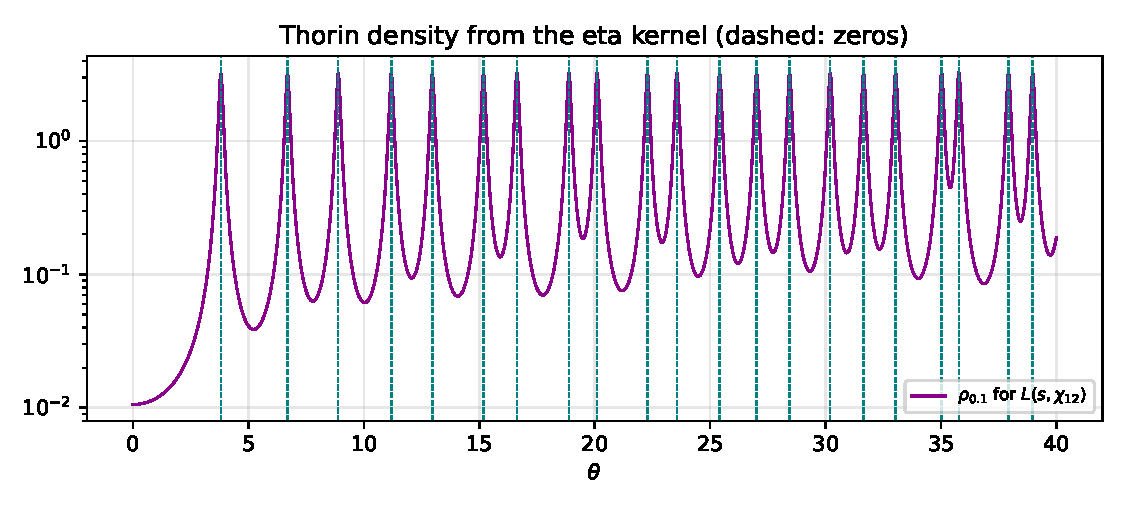
\includegraphics[width=0.95\textwidth]{fig/chi12.pdf}
\caption{The Thorin density $\rho_{0.1}$ of $L(s,\chi_{12})$ for $0\le\theta\le40$ on a logarithmic scale, computed from the Dedekind eta kernel, with the zeros dashed.}
\label{fig:ch16:rho}
\end{figure}

The zero density identity, Proposition~\ref{prop:zerodensity}, holds for $\xi(s,\chi_{12})$ with the same proof, since $\xi(s,\chi_{12})$ is entire, satisfies $\xi(s,\chi_{12})=\xi(1-s,\chi_{12})$, is positive on the real axis because $K$ is, and has no zeros with $\re s\ge1$. Its hypotheses are also the same: $T$ is not an ordinate, and no zero of $\xi(s,\chi_{12})$ lies on the segment from $\frac12+\varepsilon$ to $\frac12+\varepsilon+iT$, which is automatic at $\varepsilon=\frac12$. In it $N_{\chi_{12}}(T)$ counts the zeros with $0<\im\rho\le T$, and $\nu(\sigma,T)$ those among them with $\re\rho>\sigma$; $M_\varepsilon(T)=\int_0^T\rho_\varepsilon(\theta)\,d\theta$ is the Thorin mass up to height $T$, and $\tau_\varepsilon(T)$ is the change of argument of $\xi(s,\chi_{12})$ from $\frac12+\varepsilon+iT$ to $\frac12+iT$, divided by $\pi$. Table~\ref{tab:ch16:zd} evaluates the identity at $T=100$.

\begin{table}[htbp]
\centering\small
\begin{tabular}{rrrr}
\toprule
$\varepsilon$ & $M_\varepsilon(100)$ & $\tau_\varepsilon(100)$ & $M_\varepsilon+\tau_\varepsilon=N-2\nu$\\
\midrule
0.5 & 67.604974186 & $-0.604974186$ & 67.00000000000003\\
0.25 & 67.476432836 & $-0.476432836$ & 67.00000000010355\\
0.1 & 67.308171973 & $-0.308171973$ & 67.00000000014663\\
0.05 & 67.185437421 & $-0.185437421$ & 67.00000000009639\\
0.02 & 67.080023774 & $-0.080023774$ & 67.00000000005207\\
\bottomrule
\end{tabular}
\caption{The zero density identity for $L(s,\chi_{12})$ at height $100$, computed from the eta kernel. The last column is $N_{\chi_{12}}(100)-2\nu(\frac12+\varepsilon,100)$; the row $\varepsilon=\frac12$ gives $N_{\chi_{12}}(100)$.}
\label{tab:ch16:zd}
\end{table}

The row $\varepsilon=\frac12$ gives $N_{\chi_{12}}(100)=67$, and with the $67$ sign changes every zero below height $100$ is simple and lies on the critical line. The other rows give $\nu(\frac12+\varepsilon,100)=0$ without using the sign changes. This is GRH for $\chi_{12}$ below height $100$, read from the eta function alone. It is computed, not certified: the argument is followed on a grid as in Section~\ref{ch:turing}, in steps of $\varepsilon/8$ up the line of evaluation and in $2000$ steps along the horizontal segment, and its increments are summed in double precision. The deviations from $67$, at most $1.5\times10^{-10}$, are far below the one half that fixes the integer. GRH for small moduli has long been verified to far greater heights by other methods, by Rumely \cite{Rumely93} and later by Platt \cite{Platt16}.

\subsection{Ramanujan's \texorpdfstring{$\Delta$}{Delta} and the cost of the three evaluators}\label{sec:ch16:delta}

The same construction works for Ramanujan's cusp form $\Delta(z)=\eta(z)^{24}=\sum_{n\ge1}\tau(n)q^n$, $q=e^{2\pi iz}$, of weight $12$ and level $1$. Its $L$ function, normalised so that the critical line is $\re s=\frac12$, is $L(s,\Delta)=\sum_{n\ge1}\tau(n)n^{-s-11/2}$, and the completed function $\xi(s,\Delta)=(2\pi)^{-s-11/2}\Gamma(s+\frac{11}2)L(s,\Delta)$ satisfies $\xi(s,\Delta)=\xi(1-s,\Delta)$, since the root number of a level one form of weight $12$ is $i^{12}=1$. The Mellin transform of $\Delta(iy)$ gives the P\'olya type representation
\begin{gather*}
\xi\Big(\frac12+s,\Delta\Big)=\int_{\R}K_\Delta(u)\,e^{su}\,du,\\
K_\Delta(u)=e^{6u}\,\Delta(ie^u)=e^{6u}e^{-2\pi e^u}\prod_{n\ge1}\big(1-e^{-2\pi ne^u}\big)^{24}.
\end{gather*}
The kernel is even because $\Delta(i/y)=y^{12}\Delta(iy)$, positive by the product formula, and analytic in the strip $|\im u|<\pi/2$, twice as wide as that of the P\'olya kernel.

We computed $\tau(n)$ for $n\le3000$, the range needed for the prime weights of Section~\ref{sec:ch16:sin2}, as the coefficients of $\eta^{24}$ with integer polynomial arithmetic (checking $\tau(2)=-24$, $\tau(3)=252$, $\tau(11)=534612$), and evaluated the kernel by its $q$ expansion for $u\ge0$ and by evenness for $u<0$. At $60$ digits, with step $1/80$ and truncation $|u|\le4$, the trapezoid evaluator finds the first zeros on the critical line at
\[
9.222379,\ 13.907550,\ 17.442777,\ 19.656513,\ 22.336104,\ \dots,
\]
in agreement with the known values \cite[modular form 1.12.a.a]{LMFDB}, and $20$ sign changes below height $50$, the number of zeros there.

\label{sec:ch16:easier}Table~\ref{tab:ch16:cmp} compares this evaluator with those for $\zeta$ and $\chi_{12}$ at the same precision. In the variables of this section their steps are $1/40$ and $1/160$, and their truncations $|u|\le6$ and $|u|\le2.5$. The settings are not matched: the truncation is far longer than $60$ digits require for $\zeta$, and too short for them for $\chi_{12}$, whose kernel is still about $10^{-16}$ at $|u|=2.5$ (Section~\ref{sec:ch16:sin2}).

\begin{table}[htbp]
\centering\small
\setlength{\tabcolsep}{4pt}
\begin{tabular}{lccc}
\toprule
 & $\zeta$ & $L(s,\chi_{12})$ & $L(s,\Delta)$\\
\midrule
kernel & \begin{tabular}[t]{@{}c@{}}theta series with\\ terms of both signs\end{tabular} & \begin{tabular}[t]{@{}c@{}}$\eta$, a positive\\ product\end{tabular} & \begin{tabular}[t]{@{}c@{}}$\eta^{24}$, a positive\\ product\end{tabular}\\
decay of $\xi$ on the critical line & $e^{-\pi t/4}$ & $e^{-\pi t/4}$ & $e^{-\pi t/2}$\\
pole of $L$ & at $s=1$ & none & none\\
degree, conductor & $1$, $1$ & $1$, $12$ & $2$, $1$\\
zeros below height 50 & 10 & 28 & 20\\
first zero & 14.134725 & 3.804628 & 9.222379\\
digits lost per unit height & 0.31 & 0.36 & 0.59\\
digits lost per zero near height 40 & about 1 & about 0.5 & about 1\\
nodes & 481 & 801 & 641\\
time per point & 9.5 ms & 12.8 ms & 10.7 ms\\
\bottomrule
\end{tabular}
\caption{The trapezoid evaluators for $\zeta$, $L(s,\chi_{12})$ and $L(s,\Delta)$ at $60$ digits, with the settings given in the text. The decay of $\xi(\frac12+it)$ is shown up to a power of $t$; the digits lost per unit height are the slope of $\log_{10}|\xi(\frac12+it)|$ between heights $10.3$ and $40.3$; the times are per point, in \texttt{mpmath}.}
\label{tab:ch16:cmp}
\end{table}

The kernels are evaluated once, before the timing, so the times measure an exponential sum over the nodes and follow the node counts of the table rather than any intrinsic difference: the theta series, the eta series and the $q$ expansion of $\Delta$ all converge geometrically, with ratio at most $e^{-2\pi}$, once the modular symmetry is used. Per unit height $\Delta$ is the most expensive, because its gamma factor $\Gamma(s+\frac{11}2)$ decays like $e^{-\pi t/2}$ on the critical line, twice as fast as the $e^{-\pi t/4}$ of $\zeta$ and $\chi_{12}$: the untilted evaluator loses asymptotically $\pi/(2\log10)=0.68$ digits per unit height against $\pi/(4\log10)=0.34$. Between heights $10$ and $40$ the powers of $t$ in the completed functions and the size of $|L|$ at the two ends give the measured rates of the table. Tilting the contour to within $\delta$ of the edge of the strip reduces the loss to about $\delta\theta/\log10$ digits at height $\theta$ (Proposition~\ref{prop:tilt}, whose proof applies to both eta kernels), so the wider strip of the $\Delta$ kernel offsets its faster decay up to a factor polynomial in $1/\delta$; we have not run the tilted evaluator for $\Delta$. Per zero $L(s,\chi_{12})$ is the cheapest: its conductor packs the zeros at low height, $28$ below height $50$ against $10$ for $\zeta$, and it loses about half a digit per zero where $\zeta$ and $\Delta$ lose about one.

\subsection{The sine squared lemma without a pole}\label{sec:ch16:sin2}

The eta based functions differ from $\zeta$ in two structural ways. Their kernels are positive for an elementary reason, a product of factors $1-q^n$ with $0<q<1$, where the positivity of the P\'olya kernel $\Phi$ needs an argument (Section~\ref{ch:clock}). And their $L$ functions are entire, so two consequences of the pole of $\zeta$ disappear: the negative pole piece of the sine squared decomposition, and the factor that Chapters~\ref{chap:rzeta} and \ref{chap:rzid} need to remove the pole, which by Proposition~\ref{rz:prop:onlyhalf} alone prevents the normalised reciprocal zeta function from being a GGC. A floor in the sense of Theorem~\ref{rz:thm:floor} is still needed for $\chi_{12}$, since its tilt, the factor $e^{-c\sqrt u}$ in the variable $u$ of the clock (written $e^{-c\sqs}$ in Section~\ref{ch:rz2}), removes the negative part of the Thorin density of the gamma factor, and the gamma factor $(12/\pi)^{s/2}\Gamma(s/2)$ of $\xi(s,\chi_{12})$ is that of $\xi$ times $12^{s/2}$: Theorem~\ref{rz:thm:gammaggc} holds for it with $c=2.6861$ replaced by $c-\frac12\log12=1.4436$. The positivity of such a floor would need an analogue of Theorem~\ref{rz:thm:id}.

For $f=\chi_{12}$ or $\Delta$ write $\xi(s,f)=L_\infty(s,f)L(s,f)$, with $L_\infty$ the gamma factor, and $-(L'/L)(s,f)=\sum_{n\ge2}\Lambda_f(n)n^{-s}$ for $\re s>1$. At a basepoint $\alpha>1$ the sine squared lemma gives, as \eqref{eq:split} does for $\zeta$,
\begin{multline*}
v_\alpha(\theta)=\re\frac{\xi'}{\xi}(\alpha+i\theta,f)=\underbrace{\frac{\xi'}{\xi}(\alpha,f)}_{\text{drift}}+\underbrace{\re\frac{L_\infty'}{L_\infty}(\alpha+i\theta,f)-\frac{L_\infty'}{L_\infty}(\alpha,f)}_{\text{archimedean}\ \ge0}\\
+\underbrace{\sum_{n\ge2}\Lambda_f(n)\,n^{-\alpha}\,2\sin^2\Big(\frac{\theta\log n}2\Big)}_{\text{primes}},
\end{multline*}
where $v_\alpha(\theta)$ is $\pi$ times the Thorin density at resolution $\alpha-\frac12$, and the archimedean piece is nonnegative because the digamma function $\psi=\Gamma'/\Gamma$ satisfies $\re\psi(x+iy)\ge\psi(x)$ for $x>0$. For $\zeta$, whose gamma factor $\pi^{-s/2}\Gamma(1+\frac s2)$ absorbs the factor $s$ of $\xi$, the remaining factor $s-1$ adds the pole piece $\re\frac1{s-1}-\frac1{\alpha-1}$, which is $-\theta^2/\big((\alpha-1)((\alpha-1)^2+\theta^2)\big)$ at $s=\alpha+i\theta$, and the identity becomes \eqref{eq:split}.

The prime weights are $\Lambda(n)=\log p$ at $n=p^k$ for $\zeta$, all positive; $\Lambda_{\chi_{12}}(p^k)=\chi_{12}(p)^k\log p$ for $\chi_{12}$, of both signs and zero at $p=2$ and $3$; and $\Lambda_\Delta(p^k)=(\alpha_p^k+\bar\alpha_p^k)\log p$ for $\Delta$, where the Satake parameters $\alpha_p$ and $\bar\alpha_p$ are the roots of $X^2-\tau(p)p^{-11/2}X+1$. Deligne's theorem $|\tau(p)|\le2p^{11/2}$ \cite{Deligne74} makes them complex conjugates of modulus one, so the weights of $\Delta$ lie in $[-2\log p,2\log p]$ and take both signs.

We computed the three decompositions at $\alpha=2$ for $0\le\theta\le40$, with prime powers up to $3000$, and compared their sum with the left side computed from the kernel. They agree to $5\times10^{-4}$ for $\zeta$ and $9\times10^{-6}$ for $\Delta$, the difference being the truncation of the prime sum. For $\chi_{12}$ the largest difference, $2.5\times10^{-5}$ at $\theta=40$, is an error of the kernel evaluator, whose truncation at $|u|\le2.5$ is too short at that height. Of the $466$ prime power weights up to $3000$, none is negative for $\zeta$, $222$ are negative for $\chi_{12}$ (whose $18$ weights at powers of $2$ and $3$ vanish) and $230$ for $\Delta$.

\begin{figure}[htbp]
\centering
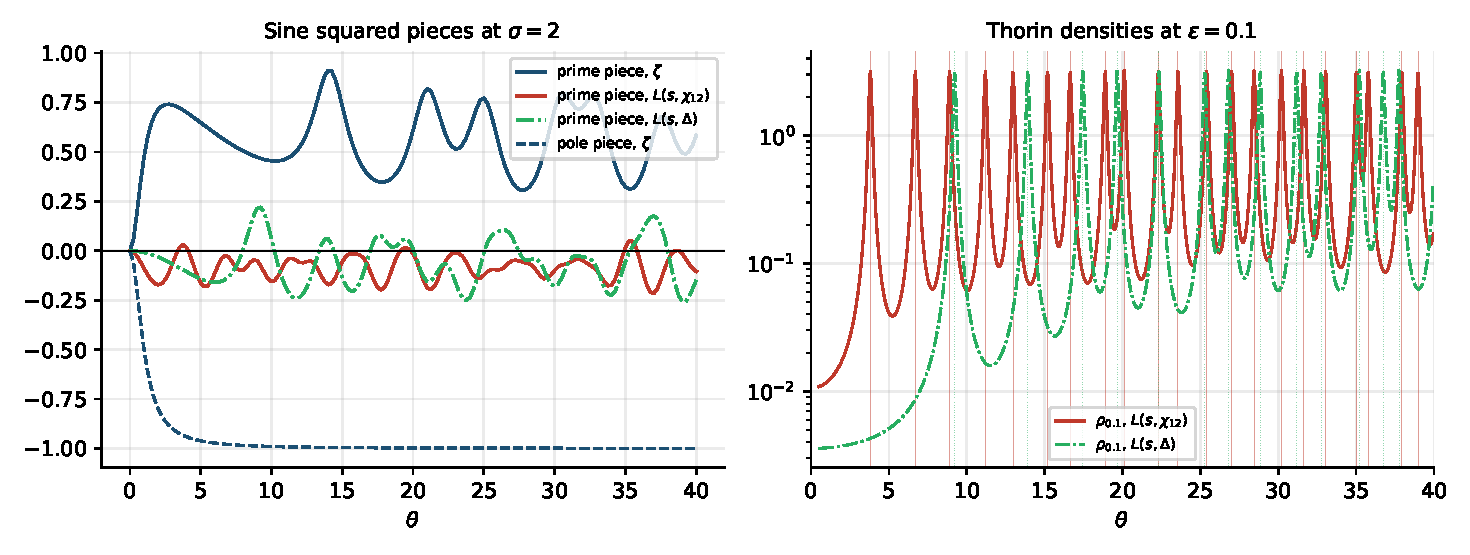
\includegraphics[width=\textwidth]{fig/lfunc.pdf}
\caption{Left: the prime pieces of the sine squared decomposition at the basepoint $\alpha=2$, written $\sigma$ in the plot, for $\zeta$, $L(s,\chi_{12})$ and $L(s,\Delta)$, and the pole piece of $\zeta$. For $\zeta$ the prime piece is positive and the pole piece negative; for the two eta based functions there is no pole piece and the prime piece takes both signs. Right: the Thorin densities $\rho_{0.1}$ of $L(s,\chi_{12})$ and $L(s,\Delta)$ on a logarithmic scale, peaking at their zeros (vertical lines).}
\label{fig:ch16:lfunc}
\end{figure}

On $0\le\theta\le40$ the prime piece of $\zeta$ ranges over $[0,0.915]$ and its pole piece over $[-0.999,0]$ (Figure~\ref{fig:ch16:lfunc}, left): the lemma writes the Thorin density as positive arithmetic mass minus one negative term. The prime piece of $L(s,\chi_{12})$ ranges over $[-0.218,0.053]$, and that of $L(s,\Delta)$ over $[-0.261,0.222]$. Their left sides are positive, with minima at $\theta=0$ equal to the drifts, $0.466$ and $0.167$, so the positivity comes from the drift and the archimedean piece, not from the primes.

For each of the three functions its Riemann hypothesis, RH for $\zeta$ and GRH for the other two, is the statement that $v_\alpha$ stays positive for every $\alpha>\frac12$; this is Lagarias's criterion \cite{Lagarias}, whose proof from the Hadamard product applies unchanged to $\xi(s,\chi_{12})$ and $\xi(s,\Delta)$. Below $\alpha=1$ the prime piece no longer converges absolutely. For $L(s,\chi_{12})$, Section~\ref{bp:eta:sec:below} shows that it still converges, as a limit over $n\le X$, when $L(s,\chi_{12})$ has no zeros to the right of some line $\re s=\alpha'$ with $\alpha'<\alpha$, and that conversely the convergence of the L\'evy form at the basepoint $\alpha$ forces the absence of zeros with $\re s>\alpha$; so the extension of the decomposition down to the centre is GRH for $\chi_{12}$. At resolution $0.1$ the Thorin densities of $L(s,\chi_{12})$ and $L(s,\Delta)$ have computed minima $0.011$ and $0.004$ below height $40$ (Figure~\ref{fig:ch16:lfunc}, right), positive as GRH predicts.

The distances of Section~\ref{ch:distances}, with the zeros of $L(s,\chi_{12})$ or $L(s,\Delta)$ as the reference atoms, Theorem~\ref{bs:thm:power} and the flow of Section~\ref{ch:dbn} carry over unchanged, the last two because they use only the Hadamard product, positivity on the real line and the decay of the kernel; we have not computed the first two for these functions, and Section~\ref{sec:ch16:dbn} computes the flow for $\Delta$. Theorem~\ref{bs:thm:power} also needs the bound $|\arg z|<\pi/4$ of Lemma~\ref{bs:lem:pair} for the zeros $z$ of $\xi(\frac12+iz,f)$ with $\re z>0$, and it holds here too: the zeros lie in the open critical strip, so $|\im z|<\frac12$, while the lowest ordinates, $3.80$ and $9.22$, exceed $\frac12$. The arithmetic side, however, offers no termwise positivity, even far to the right of the critical line, so the domination of the pole by positive primes that Sections~\ref{ch:motivation} and \ref{ch:sin2more} formulate for $\zeta$ has no direct analogue. Deligne's bound $|\Lambda_\Delta(n)|\le2\Lambda(n)$, like $|\Lambda_{\chi_{12}}(n)|\le\Lambda(n)$, bounds the prime piece below only by a multiple of minus the zeta prime piece, which tends to $-\infty$ as $\alpha\downarrow1$ for every $\theta\ne0$, and no domination argument follows from it. Far enough to the right the absolute values do suffice: the drift and the archimedean piece outweigh the prime piece bounded by the absolute values of its weights for $\alpha>1.8349$ for $L(s,\chi_{12})$ and for $\alpha>2.2823$ for the Dirichlet beta function $L(s,\chi_4)$, and by Kronecker's theorem no better bound from the sizes of the weights holds at all large heights (Propositions~\ref{prop:dbeta:termwise} and \ref{prop:dbeta:kron}). So although $L(s,\chi_{12})$ is the cheapest of the three functions per zero, neither eta based function is theoretically easier than $\zeta$: the sine squared lemma trades the negative pole term for a prime measure of both signs.

\subsection{Maxima of exponentials}\label{sec:ch16:max}

The product formula has a probabilistic reading, which the first author's note \cite{P26max} develops. The factor $1-e^{-2\pi ny}$ is the distribution function of an exponential variable with rate $2\pi n$, so
\[
F(y)=\prod_{n\ge1}\big(1-e^{-2\pi ny}\big)^{24}=e^{2\pi y}\Delta(iy),\qquad F_1(y)=\prod_{n\ge1}\big(1-e^{-2\pi ny}\big)=e^{\pi y/12}\eta(iy)
\]
are the distribution functions of the maxima $M^*$ and $M_1$ of independent exponential variables, $24$ of each rate $2\pi n$ for $M^*$ and one of each rate for $M_1$. Section~\ref{sec:maxexp:rep} turns the Mellin integral of $\Delta$ into an expectation over the law of $M^*$, a representation of $L(s,\Delta)$ with no signs, and compares it with the incomplete gamma continuations of Riemann and Hecke; Section~\ref{sec:maxexp:products} carries the construction to other products, and Section~\ref{sec:maxexp:gamma} reads it at real points as a statement about gamma mixtures. The last two parts study the laws themselves. That of $M_1$ is explicit: it is infinitely divisible, lies in the Bondesson class and is not a GGC (Section~\ref{sec:maxexp:M1}). That of $M^*$ is not even in the Bondesson class, because its Laplace transform has zeros off the real axis (Section~\ref{sec:maxexp:Mstar}).

\subsubsection{The max representation}\label{sec:maxexp:rep}

\begin{lemma}\label{lem:maxexp:max}
Let $E_{n,j}$, $n\ge1$, $1\le j\le24$, be independent, with $E_{n,j}$ exponential of rate $2\pi n$, and put $M^*=\sup_{n,j}E_{n,j}$ and $M^{(j)}=\sup_nE_{n,j}$. Almost surely these suprema are attained and finite, $\Pr(M^*\le y)=F(y)$ for $y>0$, and each $M^{(j)}$ has the distribution function $F_1$. So $M^*=\max_{j\le24}M^{(j)}$ is the maximum of $24$ independent copies of $M_1$.
\end{lemma}

\begin{proof}
For $y>0$, $\sum_{n,j}\Pr(E_{n,j}>y)=24\sum_ne^{-2\pi ny}<\infty$, so by the Borel Cantelli lemma only finitely many $E_{n,j}$ exceed $y$, almost surely. Taking $y$ rational and below $E_{1,1}$, the supremum is the largest of finitely many values. By independence $\Pr(M^*\le y)=\lim_N\prod_{n\le N}(1-e^{-2\pi ny})^{24}=F(y)$, and in the same way each $M^{(j)}$ has the distribution function $F_1$; the $M^{(j)}$ are independent because they are built from disjoint sets of the $E_{n,j}$.
\end{proof}

The modular relations $\Delta(i/y)=y^{12}\Delta(iy)$ and $\eta(i/y)=\sqrt y\,\eta(iy)$ become self dualities of the two laws,
\begin{equation}\label{eq:maxexp:dual}
F(y)=y^{-12}e^{2\pi y-2\pi/y}F(1/y),\qquad F_1(y)=y^{-1/2}e^{\pi y/12-\pi/(12y)}F_1(1/y),
\end{equation}
so the lower tails are thin: $\Pr(M^*\le y)\sim y^{-12}e^{-2\pi/y}$ and $\Pr(M_1\le y)\sim y^{-1/2}e^{-\pi/(12y)}$ as $y\downarrow0$. Since $F(1/y)\le1$, the first relation also gives $F(y)\le y^{-12}e^{2\pi y-2\pi/y}$ for every $y>0$, a bound that increases with $y$, because its logarithmic derivative is $(2\pi y^2-12y+2\pi)/y^2$ and $144<16\pi^2$.

The density of $M^*$ is Ramanujan's logarithmic derivative. Expanding $1/(1-e^{-2\pi ny})$ gives $(\log F)'(y)=24\sum_n2\pi n\,e^{-2\pi ny}/(1-e^{-2\pi ny})=48\pi\sum_{m\ge1}\sigma(m)e^{-2\pi my}$, with $\sigma(m)$ the sum of the divisors of $m$, so that, with Eisenstein's series $E_2(z)=1-24\sum_{m\ge1}\sigma(m)e^{2\pi imz}$,
\begin{equation}\label{eq:maxexp:density}
f^*(y)=F(y)\,(\log F)'(y)=2\pi F(y)\big(1-E_2(iy)\big).
\end{equation}
Taking the logarithmic derivative of \eqref{eq:maxexp:dual} gives the functional equation of the density,
\[
f^*(1/y)=y^{12}e^{2\pi/y-2\pi y}\Big(\big(2\pi y^2-12y+2\pi\big)F(y)-y^2f^*(y)\Big),
\]
which in terms of $E_2$ is its quasi modularity, $E_2(i/y)=-y^2E_2(iy)+6y/\pi$. At $y=2$ the quotient $F'/F$ of the product, the form \eqref{eq:maxexp:density} and the functional equation applied at $y=\frac12$ give the same value, $f^*(2)=0.000525840326953580416712$, and the density integrates to one to the $30$ digits printed (\texttt{maxexp\_checks.py}).

\begin{theorem}\label{thm:maxexp:max}
For every complex $s$,
\begin{equation}\label{eq:ch16:max}
\xi(s,\Delta)=(2\pi)^{-s-\frac{11}2}\,\E\,\Gamma\big(s+\tfrac{11}2,2\pi M^*\big),\qquad L(s,\Delta)=\E\,Q\big(s+\tfrac{11}2,2\pi M^*\big),
\end{equation}
with $\Gamma(a,x)=\int_x^\infty e^{-v}v^{a-1}dv$ and $Q(a,x)=\Gamma(a,x)/\Gamma(a)$, and both expectations converge absolutely. In particular $L(s,\Delta)=0$ at the points $s=-\frac{11}2-k$, $k=0,1,2,\dots$, where $Q(-k,x)=0$.
\end{theorem}

\begin{proof}
Put $a=s+\frac{11}2$, so that $\xi(s,\Delta)=\int_0^\infty\Delta(iy)y^{a-1}dy$. Inserting $\Delta(iy)=e^{-2\pi y}\Pr(M^*\le y)=e^{-2\pi y}\E\,\mathbf 1\{M^*\le y\}$ and integrating in $y$ first gives $\E\int_{M^*}^\infty e^{-2\pi y}y^{a-1}dy=(2\pi)^{-a}\E\,\Gamma(a,2\pi M^*)$. Fubini's theorem applies: with $\sigma=\re a$, Tonelli's theorem gives $\E\int_{M^*}^\infty e^{-2\pi y}y^{\sigma-1}dy=\int_0^\infty\Delta(iy)y^{\sigma-1}dy$, which is finite for every real $\sigma$, since $\Delta(iy)$ decays exponentially as $y\to\infty$ and like $y^{-12}e^{-2\pi/y}$ as $y\downarrow0$. The same computation gives $\E|\Gamma(a,2\pi M^*)|\le\E\,\Gamma(\sigma,2\pi M^*)<\infty$. Dividing by $(2\pi)^{-a}\Gamma(a)$, with $1/\Gamma$ entire, gives the second identity, in which $Q(a,x)$, for fixed $x>0$, is the entire function $\Gamma(a,x)/\Gamma(a)$ of $a$. At $a=-k$ it vanishes, since $\Gamma(-k,x)$ is finite and $1/\Gamma(-k)=0$.
\end{proof}

\begin{corollary}[Gamma mixture and mixed Poisson forms]\label{cor:maxexp:forms}
Let $G_a$ be a gamma variable of shape $a>0$ and scale one, and $N$ a Poisson process of unit rate, both independent of $M^*$. For real $s>-\frac{11}2$, with $a=s+\frac{11}2$,
\[
L(s,\Delta)=\Pr\big(G_a>2\pi M^*\big)=\E F\Big(\frac{G_a}{2\pi}\Big)=\E\prod_{n\ge1}\big(1-e^{-nG_a}\big)^{24},
\]
and for every integer $k\ge1$
\[
L\big(k-\tfrac{11}2,\Delta\big)=\Pr\big(N(2\pi M^*)\le k-1\big)=\E\Big[e^{-2\pi M^*}\sum_{j<k}\frac{(2\pi M^*)^j}{j!}\Big].
\]
\end{corollary}

\begin{proof}
For real $a>0$, $Q(a,x)=\Pr(G_a>x)$, which gives the first form; conditioning on $G_a$ instead gives $\Pr(M^*<G_a/2\pi)=\E F(G_a/2\pi)$, since the law of $M^*$ has no atoms. For an integer $k$ the $k$th point of $N$ has the law of $G_k$, so $\Pr(G_k>x)=\Pr(N(x)\le k-1)$. As a check, $F(y)=\sum_{n\ge1}\tau(n)e^{-2\pi(n-1)y}$ and $\E e^{-(n-1)G_a}=n^{-a}$ return the Dirichlet series $\sum_n\tau(n)n^{-a}$ term by term when $a>\frac{13}2$, where it converges absolutely.
\end{proof}

So $L(-\frac92,\Delta)=\E e^{-2\pi M^*}=0.03744128126851554174$ is a value of the Laplace transform of $M^*$, and the central value $L(\frac12,\Delta)=0.79212283864603056936$ is the probability that a Poisson clock of rate $2\pi$ rings at most five times before the time $M^*$. Write $P_k=\Pr(N(2\pi M^*)\le k-1)=L(k-\frac{11}2,\Delta)$. The functional equation $\xi(s,\Delta)=\xi(1-s,\Delta)$ at $s=k-\frac{11}2$ becomes the family of identities
\begin{equation}\label{eq:maxexp:fe}
(2\pi)^{-k}(k-1)!\,P_k=(2\pi)^{k-12}(11-k)!\,P_{12-k},\qquad1\le k\le11,
\end{equation}
both sides being $\xi(k-\frac{11}2,\Delta)$, which are nontrivial statements about the law of a maximum of exponential variables. Table~\ref{tab:maxexp:poisson} lists the probabilities, computed by quadrature against the density \eqref{eq:maxexp:density}; the two sides of \eqref{eq:maxexp:fe} agree to $10^{-43}$, and with Hecke's formula below to all $25$ digits printed. The gamma mixture form gives $L(0,\Delta)=\E F(G_{11/2}/2\pi)=0.7347229296103482203473$, and the max representation gives $L(\frac{17}2,\Delta)=0.998583063162746176491918$ and $L(\frac{29}2,\Delta)=0.999977182799369841174879$, in agreement with Hecke's formula and with the Dirichlet series.

\begin{table}[htbp]
\centering\small
\begin{tabular}{rcc}
\toprule
$k$ & $P_k=\Pr\big(N(2\pi M^*)\le k-1\big)=L(k-\frac{11}2,\Delta)$ & $(2\pi)^{-k}(k-1)!\,P_k=\xi(k-\frac{11}2,\Delta)$\\
\midrule
$1$ & $0.0374412812685$ & $0.00595896498958$\\
$2$ & $0.146374542091$ & $0.00370771046495$\\
$3$ & $0.315241565881$ & $0.00254175605420$\\
$4$ & $0.501617647511$ & $0.00193109920049$\\
$5$ & $0.666709188434$ & $0.00163398603484$\\
$6$ & $0.792122838646$ & $0.00154487936040$\\
$7$ & $0.877354125389$ & $0.00163398603484$\\
$8$ & $0.930707030298$ & $0.00193109920049$\\
$9$ & $0.962126459694$ & $0.00254175605420$\\
$10$ & $0.979809088251$ & $0.00370771046495$\\
$11$ & $0.989432913100$ & $0.00595896498958$\\
\bottomrule
\end{tabular}
\caption{The probabilities that a Poisson clock of rate $2\pi$ rings fewer than $k$ times before $M^*$, and the identities \eqref{eq:maxexp:fe}: the last column is symmetric about $k=6$. Computed by \texttt{maxexp\_checks.py}.}
\label{tab:maxexp:poisson}
\end{table}

\begin{remark}\label{rem:maxexp:fe}
The identities \eqref{eq:maxexp:fe} follow from the self duality \eqref{eq:maxexp:dual}, since $(2\pi)^{-k}(k-1)!\,P_k=\int_0^\infty e^{-2\pi y}F(y)y^{k-1}dy$ and the substitution $y\mapsto1/y$ turns this integral into the one with $12-k$ in place of $k$. They are five relations, since $k$ and $12-k$ give the same one and $k=6$ gives none, and they do not imply the self duality. Let $g$ be smooth and not identically zero, with compact support in $(0,1)$, such that $g(\log y)$ is orthogonal on $(1,e)$ to the five functions $e^{-2\pi y}F(y)(y^{k-1}-y^{11-k})$, $k\le5$. For small $\varepsilon$, $\tilde F(y)=F(y)\big(1+\varepsilon g(\log y)\big)$ is again a distribution function, because $F'$ has a positive lower bound and $F$ is below one on $[1,e]$, and it satisfies \eqref{eq:maxexp:fe}, because the perturbation changes the difference of the two sides of the $k$th identity by $\varepsilon$ times the integral of $g(\log y)$ against the $k$th function. It is not self dual: on $(1,e)$ self duality would give $\tilde F(y)=y^{-12}e^{2\pi y-2\pi/y}\tilde F(1/y)=F(y)$, since $g(\log(1/y))=0$. With $g$ even and supported in $(-1,1)$ instead, the same construction gives a self dual distribution function other than $F$, so self duality does not determine the law of $M^*$ either. What does determine it is self duality together with the form of $F$ as a power series in $e^{-2\pi y}$. If $F(y)=\sum_{n\ge0}c_ne^{-2\pi ny}$ for $y>0$, with $c_0=1$, and $F$ satisfies \eqref{eq:maxexp:dual}, then $f(z)=\sum_{n\ge0}c_ne^{2\pi i(n+1)z}$ is holomorphic on the upper half plane, satisfies $f(z+1)=f(z)$, and satisfies $f(-1/z)=z^{12}f(z)$ on the imaginary axis, hence everywhere by analytic continuation. So $f$ is a cusp form of weight $12$ for $\mathrm{SL}_2(\mathbb Z)$, a multiple of $\Delta$ because these cusp forms make up a space of dimension one \cite[Chapter 14]{IwaniecKowalski04}, and $c_0=1$ gives $f=\Delta$. This argument is the simplest case of Hecke's converse theorem \cite{Hecke36}, which recovers a modular form from the functional equation of its Dirichlet series. The distribution function of a maximum of independent exponential variables whose rates are integer multiples of $2\pi$ is a power series of this kind, so $M^*$ is the only such maximum with the self duality \eqref{eq:maxexp:dual}.
\end{remark}

Cutting the integral at $y=1$ and folding $(0,1)$ onto $(1,\infty)$ by modularity gives in the same way the symmetric form
\begin{gather}
\xi(s,\Delta)=A(s)+A(1-s),\qquad A(s)=\int_1^\infty\Delta(iy)\,y^{s+\frac92}dy,\label{eq:maxexp:sym}\\
A(s)=(2\pi)^{-s-\frac{11}2}\,\E\,\Gamma\big(s+\tfrac{11}2,2\pi\max(M^*,1)\big)=\sum_{n\ge1}\tau(n)\,\frac{\Gamma(s+\frac{11}2,2\pi n)}{(2\pi n)^{s+11/2}},\nonumber
\end{gather}
where the last form, Hecke's, comes from expanding $\Delta(iy)=\sum_n\tau(n)e^{-2\pi ny}$ instead. Hecke's form is the analogue for $\Delta$ of Riemann's second proof of the functional equation \cite[Chapter 1]{Edwards}, which cuts the Mellin integral of the theta function $\omega(x)=\sum_{n\ge1}e^{-\pi n^2x}$ of Section~\ref{ch:clock} at $x=1$ in the same way.

\begin{proposition}[Riemann]\label{prop:maxexp:riemann}
For every complex $s\ne0,1$,
\[
\pi^{-s/2}\Gamma\Big(\frac s2\Big)\zeta(s)=-\frac1s-\frac1{1-s}+\sum_{n\ge1}\Big[\frac{\Gamma(\frac s2,\pi n^2)}{(\pi n^2)^{s/2}}+\frac{\Gamma(\frac{1-s}2,\pi n^2)}{(\pi n^2)^{(1-s)/2}}\Big].
\]
\end{proposition}

\begin{proof}
For $\re s>1$, $\pi^{-s/2}\Gamma(\frac s2)\zeta(s)=\int_0^\infty\omega(x)x^{s/2-1}dx$. On $(0,1)$ substitute $x\mapsto1/x$ and use $\omega(1/x)=\sqrt x\,\omega(x)+\frac12\sqrt x-\frac12$, which is the theta transformation $1+2\omega(1/x)=\sqrt x\,(1+2\omega(x))$:
\[
\int_0^1\omega(x)x^{s/2-1}dx=\int_1^\infty\omega(x)x^{(1-s)/2-1}dx+\frac12\int_1^\infty x^{-(s+1)/2}dx-\frac12\int_1^\infty x^{-s/2-1}dx,
\]
and the last two integrals are $\frac1{s-1}$ and $-\frac1s$. On $(1,\infty)$ integrate $\omega$ term by term, with $\int_1^\infty e^{-\pi n^2x}x^{b-1}dx=(\pi n^2)^{-b}\Gamma(b,\pi n^2)$. The series converges uniformly on compact sets of $s$, because $\Gamma(b,\pi n^2)\le C_be^{-\pi n^2}(\pi n^2)^{\re b}$, so the identity continues to every $s\ne0,1$.
\end{proof}

At $s=2$ the right side gives $\pi/6$. At $s=\frac12+5i$ it gives a real number, as it must on the critical line, namely $-0.02182574236389736176$, and both values agree with the left side to $25$ digits. The three formulas are incomplete gamma continuations of Mellin integrals, but they randomise different things. In Riemann's and Hecke's the threshold is the fixed point $x=1$ or $y=1$, and the rates $\pi n^2$ or $2\pi n$ carry weights: one each for $\zeta$, at the price of the pole terms, and the signed coefficients $\tau(n)$ for $\Delta$. In \eqref{eq:ch16:max} there is a single rate $2\pi$, coming from the factor $q=e^{-2\pi y}$ of $\Delta$, and the threshold $M^*$ is random with a positive law; the symmetric form \eqref{eq:maxexp:sym} is Riemann's formula with the sum over $n$ replaced by an expectation over $\max(M^*,1)$, and with no pole terms. The max representation replaces Hecke's sum over the signed coefficients $\tau(n)$ by an expectation over a positive law.

The script \texttt{maxlaw.py} evaluates these expectations by quadrature against the density \eqref{eq:maxexp:density} of $M^*$ for $y\ge1$, with the self duality for $y<1$, so that $\tau$ enters only through the product. At $s=\frac12$, $\frac12+5i$ and $3$ the max representation, the symmetric form and Hecke's formula agree to the $25$ digits printed, for instance $\xi(\frac12,\Delta)=0.00154487936039502720604$. On the critical line $\xi(\frac12+i\theta,\Delta)=2\re A(\frac12+i\theta)$, and the symmetric form has its first zero at $\theta=9.2223793999211025222$. It also suggests a Hermite Biehler test, the route that Lagarias studied for $\xi$ \cite{Lagarias05}: if $|A(s)|>|A(1-s)|$ held throughout $\re s>\frac12$, there could be no zeros there. The test fails. At $\theta=0$ the half $A(s)$ dominates, with $|A(1-s)|/|A(s)|$ falling from $0.989$ at $\re s=0.52$ to $0.100$ at $\re s=4.5$, but on $\re s=0.6$ the two halves have equal modulus at $\theta=10.26$, $14.67$, $18.04$, $20.36$ and $22.99$, and the dominant half alternates between these ordinates, which separate the zeros $9.22$, $13.91$, $17.44$, $19.66$ and $22.34$. The curves of equal modulus are nearly vertical near the critical line and bend towards lower ordinates as $\re s$ grows (Figure~\ref{fig:maxexp:dominance}): on $\re s=4.5$ the first crossing is at $\theta=8.05$, and seven lie below height $25$ (\texttt{maxlaw.py}, \texttt{maxexp\_hb.py}). So the cut at $y=1$ gives no Hermite Biehler function.

The cut can be moved. For every $c>0$ the same folding gives $\xi(s,\Delta)=A_c(s)+A_{1/c}(1-s)$ with $A_c(s)=\int_c^\infty\Delta(iy)y^{s+9/2}dy$, and $c$ may be chosen separately on each horizontal ray. The script \texttt{maxexp\_hb.py} computes, for $0\le\theta\le25$ in steps of $0.05$, the best over $36$ cuts $c\in[0.35,1.2]$ of the least ratio $|A_c(s)|/|A_{1/c}(1-s)|$ over $120$ points of the ray $s=\sigma+i\theta$, $\frac12<\sigma\le14.5$. For $\theta\le12.9$ and $13.95\le\theta\le15.2$, and at $\theta=15.35$ and $15.4$, some cut dominates on the whole ray, for instance at $\theta=5$, $10.5$ and $12$ with least ratios $566$, $4.46$ and $2.03$, all for the smallest cut tried, $c=0.35$, where the cut at $1$ gives $1.0007$, $0.9065$ and $0.992$. For $12.95\le\theta\le13.9$, just below the zero $13.91$, at $\theta=15.25$ and $15.3$, and for $15.45\le\theta\le25$, no cut in the range dominates, the best least ratio staying between $0.9955$ and $1$. The freedom is in any case illusory. As $c\to0$, $A_{1/c}(1-s)\to0$ and $A_c(s)\to\xi(s,\Delta)$ uniformly on compact sets, so domination for small $c$ only says that $\xi(s,\Delta)$ does not vanish there, and the certificate turns into an evaluation of $\xi$; and at a zero $\frac12+i\gamma$ the two halves have equal modulus for every $c$, since their sum vanishes. A Hermite Biehler function that could prove GRH for $\Delta$ would have to come from the structure of the law of $M^*$, not from tuning a cut. The representation is exact and has no signs, but like the kernel it restates the problem without locating the zeros.

\begin{figure}[htbp]
\centering
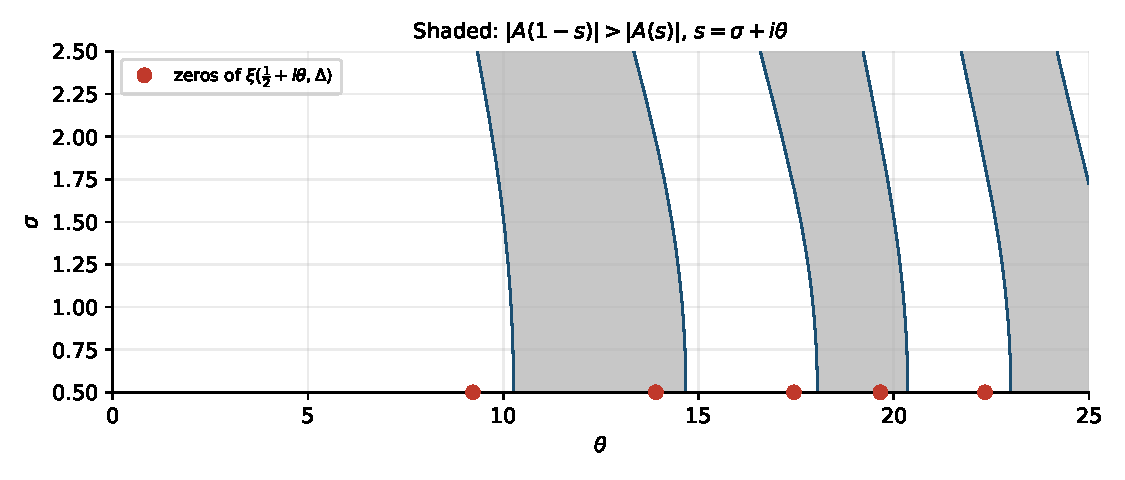
\includegraphics[width=0.8\textwidth]{fig/maxexp_dominance.pdf}
\caption{The Hermite Biehler test with the cut at $y=1$: shaded where $|A(1-s)|>|A(s)|$ for $s=\sigma+i\theta$, $\frac12<\sigma\le2.5$, with the curves of equal modulus and the zeros of $\xi(\frac12+i\theta,\Delta)$. Drawn by \texttt{maxexp\_figs.py}.}
\label{fig:maxexp:dominance}
\end{figure}

\subsubsection{Other theta products}\label{sec:maxexp:products}

The construction needs a modular form whose expansion on the imaginary axis is a power of $q$ times a product of factors $1-q^a$, $a>0$, with nonnegative exponents, so that the product is a distribution function; eta products with nonnegative exponents qualify.

For $\chi_{12}$ the Mellin integral of Section~\ref{sec:ch16:eta}, with $\eta(ix)=e^{-\pi x/12}F_1(x)$, gives in the same way
\[
L(s,\chi_{12})=\E\,Q\Big(\frac s2,\frac\pi{12}M_1\Big),\qquad\xi(s,\chi_{12})=A_{12}(s)+A_{12}(1-s),
\]
with $A_{12}(s)=\int_1^\infty\eta(ix)x^{s/2-1}dx=(\frac\pi{12})^{-s/2}\E\,\Gamma(\frac s2,\frac\pi{12}\max(M_1,1))$; the second exponent comes from $\eta(i/x)=\sqrt x\,\eta(ix)$. The factor $q^{1/24}$ of $\eta$ is what turns Euler's pentagonal exponents $k(3k\mp1)/2$ into the squares $n^2/24$, $n=6k\mp1$, and so produces the theta series, and the Dirichlet series, of a character. At $s=1$, where $Q(\frac12,x)=\operatorname{erfc}\sqrt x$, the class number formula reads $\E\operatorname{erfc}\sqrt{\pi M_1/12}=L(1,\chi_{12})=\log(2+\sqrt3)/\sqrt3$; at $s=2$, where $Q(1,x)=e^{-x}$, $L(2,\chi_{12})=\E e^{-\pi M_1/12}=\pi^2/(6\sqrt3)$ is a value of the Laplace transform of $M_1$, which Section~\ref{sec:maxexp:M1} computes in closed form; and at the centre $L(\frac12,\chi_{12})=\Pr(12G_{1/4}>\pi M_1)=0.498557002457815436157$. At $s=0.6+5i$ the max representation, both forms of the symmetric form and \texttt{mpmath}'s Dirichlet $L$ function agree to $25$ digits, with $\xi(0.6+5i,\chi_{12})$ as in Section~\ref{sec:ch16:eta}, and so do the three values above with their closed forms (\texttt{maxexp\_checks.py}, \texttt{maxlaw.py}).

For the elliptic curve of conductor $11$ the newform is $f(z)=\eta(z)^2\eta(11z)^2=q\prod_{n\ge1}(1-q^n)^2(1-q^{11n})^2=\sum_{n\ge1}a_nq^n$ \cite[modular form 11.2.a.a]{LMFDB}, so $f(iy)=e^{-2\pi y}F_{11}(y)$, where $F_{11}$ is the distribution function of the maximum $M_{11}$ of independent exponential variables, two of each rate $2\pi n$ and two of each rate $22\pi n$. The Fricke relation $f(i/(11y))=11y^2f(iy)$ makes $f(iy)$ decay faster than any power at both ends, and the proof of Theorem~\ref{thm:maxexp:max} gives, in the arithmetic normalisation $L(s,E)=\sum_na_nn^{-s}$ with centre $s=1$,
\[
L(s,E)=\E\,Q(s,2\pi M_{11})\quad\text{for every complex }s,\qquad L(1,E)=\E e^{-2\pi M_{11}}.
\]
So the central value is a value of the Laplace transform of $M_{11}$, and the max representation gives $L(1,E)=0.2538418608559106843378$, equal to all digits to the rapidly convergent series $2\sum_na_nn^{-1}e^{-2\pi n/\sqrt{11}}$ of root number one.

Jacobi's triple product gives $\vartheta_4(x)=\sum_{n\in\mathbb Z}(-1)^ne^{-\pi n^2x}=\prod_{m\ge1}(1-e^{-2\pi mx})(1-e^{-\pi(2m-1)x})^2$, a distribution function with no prefactor: that of the maximum $M_4$ of independent exponential variables, one of each rate $2\pi m$ and two of each rate $\pi(2m-1)$. The partial sums of the alternating series lie between $-1$ and $1$, so the series can be integrated term by term against $\theta e^{-\theta y}$, and the partial fraction expansion of $z/\sinh z$ gives
\[
\E e^{-\theta M_4}=\sum_{n\in\mathbb Z}(-1)^n\frac\theta{\theta+\pi n^2}=\frac{\sqrt{\pi\theta}}{\sinh\sqrt{\pi\theta}}=\prod_{n\ge1}\Big(1+\frac\theta{\pi n^2}\Big)^{-1},
\]
so $M_4\overset d=\sum_{n\ge1}E_n/(\pi n^2)$ with independent standard exponential variables $E_n$: a maximum of exponential variables that is also a sum of them, and a GGC with Thorin measure $\sum_n\delta_{\pi n^2}$. Since $\Pr(K\le k)=\sum_n(-1)^ne^{-2n^2k^2}=\vartheta_4(2k^2/\pi)$, $\pi M_4=2K^2$ has the Kolmogorov law of Table~\ref{tab:ch3:cat}. With no prefactor the Mellin transform gives moments instead of incomplete gamma functions: $\E M_4^{s/2}=\frac s2\int_0^\infty y^{s/2-1}(1-\vartheta_4(y))\,dy$ for $\re s>0$, and integrating $1-\vartheta_4(y)=2\sum_{n\ge1}(-1)^{n+1}e^{-\pi n^2y}$ term by term, for $\re s>1$ and then by analytic continuation, gives
\[
(1-2^{1-s})\,\zeta(s)=\frac{\E\big[(2K^2)^{s/2}\big]}{2\,\Gamma(1+\frac s2)}
\]
for every complex $s$, both sides being entire, since $\vartheta_4(y)=y^{-1/2}\sum_ne^{-\pi(n+\frac12)^2/y}$ makes every moment of $M_4$ finite. This is a case of the dictionary of Biane, Pitman and Yor \cite{BPY01}. At $s=1$ it gives $\E K=\sqrt{\pi/2}\,\log2=0.868731160636159141830$, which quadrature of $1-\vartheta_4$ reproduces to $2\times10^{-23}$; at $s=3$ and $\frac12+5i$ the two sides agree to $25$ digits, and $\E e^{-3M_4}=\sqrt{3\pi}/\sinh\sqrt{3\pi}=0.285645278943791835551$ by quadrature and in closed form.

For $\zeta$ itself the construction stops. The theta function $\vartheta_3(x)=1+2\omega(x)=\prod_{m\ge1}(1-q^{2m})(1+q^{2m-1})^2$, $q=e^{-\pi x}$, has factors larger than one and is not a distribution function, and the transformation $\vartheta_4(1/x)=\sqrt x\,\vartheta_2(x)$ leads to $\vartheta_2(x)=\sum_ne^{-\pi(n+\frac12)^2x}$, which is not one either. So the max structure reaches $\zeta$ only through the factor $1-2^{1-s}$, in moment form. It does not reach it through $\zeta_{\mathbb Q(\sqrt3)}(s)=\zeta(s)L(s,\chi_{12})$: the eta law represents the factor $L(s,\chi_{12})$ only, and no product of this kind can represent a Dedekind zeta function, since an eta product with nonnegative exponents decays faster than any power of $y$ at both ends of the imaginary axis, so its Mellin transform is entire, as in the proof of Theorem~\ref{thm:maxexp:max}, while $\zeta_{\mathbb Q(\sqrt3)}$ has a pole at $s=1$.

\subsubsection{Gamma shapes and infinite divisibility at real points}\label{sec:maxexp:gamma}

The P\'olya kernel of $\zeta$ and the kernel $K_\Delta$ of $\Delta$ differ in their gamma shapes. On the logarithmic scale the function $x^ae^{-x}$ of $x=ce^{ku}$ is proportional to the density of $(\log G_a-\log c)/k$, a log gamma density of shape $a$, and its Fourier transform $\int_{\R}x^ae^{-x}e^{i\theta u}du=k^{-1}c^{-i\theta/k}\Gamma(a+i\theta/k)$ has no zeros. With $x=2\pi e^u$, $K_\Delta(u)=e^{6u}\Delta(ie^u)=(2\pi)^{-6}x^6e^{-x}F(e^u)$ is a single gamma kernel of shape $6$ times the distribution function of $\log M^*$, and the gamma kernel's own transform is $(2\pi)^{-6-i\theta}\Gamma(6+i\theta)$, so every zero of $\xi(\frac12+i\theta,\Delta)$ is produced by the multiplier $F(e^u)$. The P\'olya kernel \eqref{eq:ch2:Phi} is, with $x_n=\pi n^2e^{2u}$ and the gamma densities $g_k(x)=x^{k-1}e^{-x}/\Gamma(k)$,
\[
\Phi(u)=2e^{u/2}\sum_{n\ge1}\big(2x_n^2-3x_n\big)e^{-x_n}=2e^{u/2}\sum_{n\ge1}\big(4g_3(x_n)-3g_2(x_n)\big),
\]
a signed mixture of Gamma(2) and Gamma(3) densities over the scales $\pi n^2$. As a function of $x=e^{2u}$ the sum is, up to the factor $x/2$, the density $2\sum_n(2\pi^2n^4x-3\pi n^2)e^{-\pi n^2x}$ of $\pi S_2/2$ in the representation $2\xi(s)=\E[(\pi S_2/2)^{s/2}]$ of Williams and of Biane, Pitman and Yor (Section~\ref{sec:ch19:williams}): a positive density that is a signed sum of gamma densities. On the logarithmic scale, with the weight $e^{u/2}=(x_n/\pi n^2)^{1/4}$, the two terms have shapes $\frac94$ and $\frac54$, while the theta function itself contributes $x_n^{1/4}e^{-x_n}$, of shape $\frac14$. The next remark shows where the two extra units come from.

\begin{remark}\label{rem:maxexp:shapes}
Let $D=-x\,d/dx$. Integrating by parts, $\int_0^\infty(Df)(x)x^{s/2-1}dx=\frac s2\int_0^\infty f(x)x^{s/2-1}dx$ whenever the boundary terms vanish, so the operator $2D(D-\frac12)$ corresponds to the factor $\frac12s(s-1)$ of $\xi(s)=\frac12s(s-1)\pi^{-s/2}\Gamma(\frac s2)\zeta(s)$. It annihilates $-\frac12$ and $\frac12x^{-1/2}$, the two terms by which $\omega(x)$ and $x^{-1/2}\omega(1/x)$ differ, and it maps $e^{-x}$ to $(2x^2-3x)e^{-x}$. Hence $[2D(D-\frac12)\omega](x)$, which is also $2D(D-\frac12)$ applied to $x^{-1/2}\omega(1/x)$, decays faster than any power at both ends,
\begin{gather*}
\xi(s)=\int_0^\infty\big[2D(D-\tfrac12)\omega\big](x)\,x^{s/2-1}dx\quad\text{for every }s,\\
\Phi(u)=2e^{u/2}\big[2D(D-\tfrac12)\omega\big](e^{2u}),
\end{gather*}
the first for $\re s>1$ by the integration by parts and then for every $s$ by analytic continuation, and the second by $x=e^{2u}$. So the gamma shapes of the terms $e^{-\pi n^2x}$ of $\omega$, one in $x$ and $\frac14$ on the logarithmic scale, are raised by one and by two, to the Gamma(2) and Gamma(3) of the P\'olya kernel, by the operator that removes the poles of $\zeta$. For $\Delta$, whose $L$ function is entire, no such operator is needed and the kernel keeps the single shape $6$; the cancellation between the Gamma(2) and Gamma(3) terms of $\Phi$ is replaced by the positive multiplier $F(e^u)$.
\end{remark}

At real points the Gamma(2) shape enters in a different way, through Kristiansen's theorem \cite{Kristiansen94}: every scale mixture of Gamma(2) laws, the law of $G_2V$ with $V\ge0$ independent of $G_2$, is infinitely divisible. Since $G_a\overset d=G_2B$ for $0<a<2$, with $B$ a beta variable of parameters $a$ and $2-a$ independent of $G_2$, the scale mixtures of Gamma($a$) laws with $a\le2$ are scale mixtures of Gamma(2) laws.

\begin{proposition}\label{prop:maxexp:krist}
For real $a>0$ let $W_a=G_a/(2\pi M^*)$, with $G_a$ independent of $M^*$. Then $W_a$ is a scale mixture of Gamma($a$) laws, the mixing law being that of $1/(2\pi M^*)$, and $L(a-\frac{11}2,\Delta)=\Pr(W_a>1)$. For $0<a\le2$, that is $-\frac{11}2<s\le-\frac72$, $W_a$ is infinitely divisible. In the same way $L(s,\chi_{12})=\Pr\big(12G_{s/2}/(\pi M_1)>1\big)$ for real $s>0$, where $12G_{s/2}/(\pi M_1)$ is infinitely divisible for $s\le4$, and is a mixture of exponential laws for $s\le2$, in particular at the centre $s=\frac12$.
\end{proposition}

\begin{proof}
The identities are Corollary~\ref{cor:maxexp:forms} and its analogue for $M_1$. For $a\le2$, $W_a=G_2\cdot B/(2\pi M^*)$ is a scale mixture of Gamma(2) laws, infinitely divisible by Kristiansen's theorem. For $s\le2$, $G_{s/2}\overset d=G_1B'$ with $B'$ a beta variable of parameters $\frac s2$ and $1-\frac s2$ (or $B'=1$ at $s=2$), so $12G_{s/2}/(\pi M_1)$ is a scale mixture of exponential laws, which is infinitely divisible by the theorem of Goldie and Steutel \cite{Goldie67,Steutel67}.
\end{proof}

At $a=2$ the proposition reads $L(-\frac72,\Delta)=\Pr(W_2>1)=\E\big[(1+2\pi M^*)e^{-2\pi M^*}\big]=0.146374542091266$, the Gamma(2) survival function averaged over $2\pi M^*$ (Table~\ref{tab:maxexp:poisson}). The proposition says nothing about zeros: the representation $\Pr(W_a>1)$ holds for real $a$ only, since on the critical line the shape $6+i\theta$ is not that of a probability law; for $\Delta$ the centre $a=6$ lies outside Kristiansen's range, while for $\chi_{12}$ the centre shape $\frac14$ lies inside it. The two Gamma(2) structures are also different in kind: the one in the P\'olya kernel is a kernel shape forced by the poles of $\zeta$, which governs the integrand on the critical line, and the one in Proposition~\ref{prop:maxexp:krist} is a mixing law, which governs a value at a real point.

\subsubsection{The law of \texorpdfstring{$M_1$}{M1}}\label{sec:maxexp:M1}

The law of $M_1$ is explicit. Put $b_n=\pi(n^2-1)/12$; the pentagonal number theorem of Section~\ref{sec:ch16:eta} reads $F_1(y)=\sum_{n\ge1}\chi_{12}(n)e^{-b_ny}$, so the rates in this expansion are $b_{6k\pm1}=\pi k(3k\pm1)$, $2\pi$ times the generalised pentagonal numbers $k(3k\pm1)/2$.

\begin{proposition}\label{prop:ch16:M1}
For $\theta>0$ let $w=\sqrt{1-12\theta/\pi}$, positive or purely imaginary. Then
\[
\E e^{-\theta M_1}=\frac{\pi(1-w^2)\sin(\pi w/3)}{2\sqrt3\,w\cos(\pi w/2)}=\prod_{k\ge1}\frac{1+\theta/b_{6k}}{(1+\theta/b_{6k-1})(1+\theta/b_{6k+1})}.
\]
\end{proposition}

\begin{proof}
Since $\sum_n\theta/(\theta+b_n)<\infty$, $\theta e^{-\theta y}F_1(y)$ can be integrated term by term, and $\theta+b_n=\pi(n^2-w^2)/12$ gives $\E e^{-\theta M_1}=\sum_{n\ge1}\chi_{12}(n)\theta/(\theta+b_n)=(1-w^2)\sum_{n\ge1}\chi_{12}(n)/(n^2-w^2)$. The function $g(w)=\pi\sin(\pi w/3)/(2\sqrt3\,w\cos(\pi w/2))$ is even and meromorphic, its only poles are simple and at the odd integers prime to $3$, and its residue at $w=n$ is $-\chi_{12}(n)/(2n)$, as for the series, so their difference is entire. On the circles $|w|=2k$, $|\cos(\pi w/2)|$ is bounded below, so $g=O(1/k)$ there, and the series is $O(k^{-1}\log k)$; by the maximum modulus principle the difference vanishes. For the product, insert $\sin(\pi w/3)=\frac{\pi w}3\prod_{m\ge1}(1-\frac{w^2}{9m^2})$ and $\cos(\pi w/2)=\prod_{n\text{ odd}}(1-\frac{w^2}{n^2})$. The factors with $n=3m$, $m$ odd, cancel, $1-w^2$ cancels the factor $n=1$, and what remains is a constant times the factors $1-w^2/n^2$ with $n=6k$ above and $n=6k\pm1$ below. The value $1$ at $\theta=0$ fixes the constant, and $(1-w^2/n^2)/(1-1/n^2)=1+\theta/b_n$.
\end{proof}

At $\theta=\pi/12$, where $w=0$, the closed form gives $\E e^{-\pi M_1/12}=\pi^2/(6\sqrt3)$, which is $L(2,\chi_{12})$ by Section~\ref{sec:maxexp:products}; the series in the proof reduces to $\sum_n\chi_{12}(n)n^{-2}$ there.

\begin{corollary}[A R\'enyi type identity]\label{cor:maxexp:renyi}
$M_1\overset d=\sum_{k\ge1}Y_k$ with independent $Y_k$, where $Y_k$ is exponential of rate $b_{6k-1}$ with probability $p_k$ and of rate $b_{6k+1}$ with probability $1-p_k$, and
\[
p_k=\Big(1-\frac{b_{6k-1}}{b_{6k}}\Big)\frac{b_{6k+1}}{b_{6k+1}-b_{6k-1}}=\frac{(12k-1)(3k+1)}{2(36k^2-1)},
\]
so $p_1=\frac{22}{35}$, $p_2=\frac{161}{286}$, and $p_k\downarrow\frac12$.
\end{corollary}

\begin{proof}
For $\alpha<\gamma<\beta$ the partial fractions $\frac{1+\theta/\gamma}{(1+\theta/\alpha)(1+\theta/\beta)}=p\frac\alpha{\alpha+\theta}+(1-p)\frac\beta{\beta+\theta}$ hold with $p=(1-\alpha/\gamma)\beta/(\beta-\alpha)$ and $1-p=\alpha(\beta-\gamma)/(\gamma(\beta-\alpha))$, both in $(0,1)$; take $\alpha=b_{6k-1}=\pi k(3k-1)$, $\gamma=b_{6k}=\pi(36k^2-1)/12$ and $\beta=b_{6k+1}=\pi k(3k+1)$ in each factor of Proposition~\ref{prop:ch16:M1}, and use the continuity theorem for Laplace transforms.
\end{proof}

By Frullani's integral, as in the first reading of Section~\ref{sec:ch3:readings}, the product gives
\[
-\log\E e^{-\theta M_1}=\int_0^\infty\big(1-e^{-\theta t}\big)\frac{k_1(t)}t\,dt,\quad k_1(t)=\sum_{k\ge1}\big(e^{-b_{6k-1}t}+e^{-b_{6k+1}t}-e^{-b_{6k}t}\big),
\]
so $M_1$ is infinitely divisible, with no drift and L\'evy density $k_1(t)/t$; this also follows from Corollary~\ref{cor:maxexp:renyi}, since mixtures of exponential laws are infinitely divisible \cite{Goldie67,Steutel67}. The L\'evy density is completely monotone, since $(e^{-b_{6k-1}t}-e^{-b_{6k}t})/t=\int_{b_{6k-1}}^{b_{6k}}e^{-zt}dz$, so $M_1$ lies in the Bondesson class BO of Section~\ref{sec:ch3:hierarchy}. It is not a GGC: its Thorin measure would have to be $U_1=\sum_k(\delta_{b_{6k-1}}+\delta_{b_{6k+1}}-\delta_{b_{6k}})$, negative at the points $b_{6k}$ where $\chi_{12}$ vanishes between $6k-1$ and $6k+1$. Concretely, the transform vanishes at $\theta=-b_{6k}$, where $w=6k$, so $-(\log\E e^{-\theta M_1})'$ has residue $-1$ there, and if $M_1$ were a GGC the Stieltjes inversion \eqref{eq:ch3:inversion} of this function would give $U(\{b_{6k}\})=-1$. The poles of the transform are at $\theta=-b_n$, $n\equiv\pm1\pmod6$, $n\ge5$, and its zeros at $-b_{6k}$: each zero lies between its own two poles $-b_{6k\pm1}$, but zeros and poles do not alternate, since $-b_7$ and $-b_{11}$, for instance, are consecutive poles. The next lemma, the Frullani identity behind Lemma~\ref{rz:lem:sin2} and the cosine dictionary \eqref{rz:eq:cosdict} read for a signed Thorin measure, turns this sign structure into a positivity statement.

\begin{lemma}\label{lem:maxexp:dict}
Let $X\ge0$ have Laplace exponent $-\log\E e^{-\theta X}=\int_{(0,\infty)}\log(1+\theta/z)\,U(dz)$ for a signed measure $U$ with $\int\log(1+1/z)\,|U|(dz)<\infty$, and put $N(z)=U((0,z])$, with $N(z)\log(1+u^2/z^2)\to0$ as $z\to\infty$ for real $u$. Then $-\log\E e^{-\theta X}=\int_0^\infty(1-e^{-\theta t})\nu(t)\,dt$ for $\theta\ge0$, with the signed function $\nu(t)=t^{-1}\int e^{-zt}U(dz)=\int_0^\infty e^{-zt}N(z)\,dz$, and for real $u$
\begin{equation}\label{eq:maxexp:three}
\begin{aligned}
-\log\big|\E e^{iuX}\big|^2&=\int_0^\infty4\sin^2\Big(\frac{ut}2\Big)\nu(t)\,dt\\
&=\int\log\Big(1+\frac{u^2}{z^2}\Big)U(dz)=\int_0^\infty N(z)\,\frac{2u^2}{z(z^2+u^2)}\,dz .
\end{aligned}
\end{equation}
The law of $X$ is a GGC if and only if $U\ge0$, and it lies in BO, that is, it is infinitely divisible with a completely monotone L\'evy density, if and only if $N\ge0$.
\end{lemma}

\begin{proof}
Frullani's integral $\log(1+\theta/z)=\int_0^\infty(1-e^{-\theta t})e^{-zt}t^{-1}dt$ gives the L\'evy form, the exchange of integrals being justified by $\log(1+\theta/z)\le C_\theta\log(1+1/z)$, and integrating $e^{-zt}$ against $dN$ by parts gives the second expression of $\nu$. The first equality of \eqref{eq:maxexp:three} is twice the real part of the L\'evy form at $\theta=-iu$, since $1-\cos ut=2\sin^2(ut/2)$; the second is the Frullani identity $\int_0^\infty4\sin^2(ut/2)e^{-zt}t^{-1}dt=\log(1+u^2/z^2)$; the third is an integration by parts, with $\frac d{dz}\log(1+u^2/z^2)=-2u^2/(z(z^2+u^2))$, whose boundary terms vanish by the assumptions. The signed function $\nu$ is determined by the law of $X$, since $t\nu(t)$ is the inverse Laplace transform of the derivative of $-\log\E e^{-\theta X}$, and so is the signed measure $U$, by the Stieltjes inversion of $\int U(dz)/(\theta+z)$. If $U\ge0$ the law is a GGC, and if it is a GGC, its Laplace exponent grows more slowly than $\theta$, so it has no drift, and its Thorin measure is $U$. If $N\ge0$, $\nu$ is completely monotone and the law is in BO; if the law is in BO, its L\'evy density is $\int e^{-zt}\mu(dz)$ with $\mu\ge0$, it equals $\nu$, and the uniqueness of Laplace transforms gives $\mu(dz)=N(z)\,dz$, so $N\ge0$, $N$ being right continuous.
\end{proof}

For $M_1$ the Thorin measure is $U_1=\sum_{n\ge2}a(n)\delta_{b_n}$ with weights of sine squared form,
\[
a(n)=\sin^2\frac{\pi n}2+\frac43\sin^2\frac{\pi n}3-1=\mathbf 1\{2\nmid n\}-\mathbf 1\{3\mid n\}=\frac16-\frac12\cos\pi n-\frac23\cos\frac{2\pi n}3,
\]
equal to $1$ for $n\equiv\pm1\pmod6$, to $-1$ for $6\mid n$, and to $0$ otherwise; each sine square is a combination of additive characters of $\mathbb Z/2$ or $\mathbb Z/3$, which makes Poisson summation available.

\begin{proposition}\label{prop:maxexp:levy}
The canonical function $k_1(t)=t\nu_1(t)$ of $M_1$ has the theta form
\[
k_1(t)=\tfrac12e^{\pi t/12}\Big(1+\frac{\vartheta_0-3\vartheta_{1/2}-4\vartheta_{1/3}}{\sqrt{3t}}\Big)-1,\qquad \vartheta_\alpha=\sum_{m\in\mathbb Z}e^{-12\pi(m+\alpha)^2/t},
\]
so $\nu_1(t)=(2\sqrt3)^{-1}t^{-3/2}-(2t)^{-1}+O(t^{-1/2})$ as $t\downarrow0$ and $\nu_1(t)\sim e^{-2\pi t}/t$ as $t\to\infty$. Its Bondesson function $N_1(z)=U_1((0,z])$ is nonnegative, and $N_1(z)\sim\frac13\sqrt{3z/\pi}$ as $z\to\infty$.
\end{proposition}

\begin{proof}
Since $a$ is even, $a(0)=-1$ and $a(1)=1$,
\[
k_1(t)=\sum_{n\ge2}a(n)e^{-b_nt}=\tfrac12e^{\pi t/12}\Big(1+\sum_{n\in\mathbb Z}a(n)e^{-\pi n^2t/12}\Big)-1.
\]
Poisson summation, $\sum_{n\in\mathbb Z}\cos(2\pi n\alpha)e^{-\pi n^2v}=v^{-1/2}\sum_{m\in\mathbb Z}e^{-\pi(m+\alpha)^2/v}$ with $v=t/12$, applied to the three terms of the cosine form of $a(n)$, gives the theta form. As $t\downarrow0$, $\vartheta_0=1+O(e^{-12\pi/t})$, while $\vartheta_{1/2}$ and $\vartheta_{1/3}$ are $O(e^{-4\pi/(3t)})$, so $k_1(t)=(2\sqrt{3t})^{-1}-\frac12+O(\sqrt t)$; as $t\to\infty$ the first term $e^{-b_5t}=e^{-2\pi t}$ of the series dominates. Since $b_{6k-1}<b_{6k}<b_{6k+1}$, every negative atom of $U_1$ is preceded by its own positive atom, so $N_1\ge0$. Up to $z$ there are about $X/3$ integers $n\equiv\pm1\pmod6$ and $X/6$ multiples of $6$ with $b_n\le z$, where $X=\sqrt{12z/\pi+1}$, so $N_1(z)=X/6+O(1)\sim\frac13\sqrt{3z/\pi}$; this agrees with the expansion at $0$, since $\nu_1(t)=\int_0^\infty e^{-zt}N_1(z)\,dz$ and $c\sqrt z$ gives $c\,\Gamma(\frac32)t^{-3/2}$.
\end{proof}

The L\'evy density has the index $\frac12$ of a Brownian first passage time, matching $-\log\E e^{-\theta M_1}\sim\sqrt{\pi\theta/3}$, which the lower tail $F_1(y)\sim y^{-1/2}e^{-\pi/(12y)}$ gives; this index comes from modularity. By \eqref{eq:maxexp:three}, the modulus of the characteristic function is
\[
\big|\E e^{iuM_1}\big|^{-2}=\prod_{k\ge1}\frac{(1+u^2/b_{6k-1}^2)(1+u^2/b_{6k+1}^2)}{1+u^2/b_{6k}^2}=\exp\int_0^\infty N_1(z)\,\frac{2u^2\,dz}{z(z^2+u^2)},
\]
the exponential of a positive kernel integrated against a nonnegative function. Figure~\ref{fig:maxexp:laws} (left) shows $N_1$ against its asymptote.

The sine squared form of $a(n)$ splits $U_1$ into two positive measures: $\sin^2(\pi n/2)$ selects the odd $n$, and $1-\frac43\sin^2(\pi n/3)$ the multiples of $3$. Each is the Thorin measure of a GGC.

\begin{theorem}\label{thm:maxexp:ggc}
With independent standard exponential variables $E_n$ and $E'_m$, let $S=\sum_{n\text{ odd},\,n\ge3}E_n/b_n$ and $Z=\sum_{m\ge1}E'_m/b_{3m}$, with $Z$ independent of $M_1$. Then $S$ and $Z$ are GGCs,
\[
\E e^{-\theta S}=\frac\pi4\,\frac{1-w^2}{\cos(\pi w/2)},\qquad \E e^{-\theta Z}=\frac{\sqrt3\,w/2}{\sin(\pi w/3)},
\]
and $M_1+Z\overset d=S$. Equivalently $U_1=U_S-U_Z$, with $U_S=\sum_{n\text{ odd},\,n\ge3}\delta_{b_n}$ and $U_Z=\sum_{m\ge1}\delta_{b_{3m}}$, the atoms at $b_{3m}$ with $m$ odd cancelling.
\end{theorem}

\begin{proof}
With $1+\theta/b_n=(n^2-w^2)/(n^2-1)$, the product $\cos(\pi w/2)=\prod_{n\text{ odd}}(1-w^2/n^2)$ gives $\prod_{n\text{ odd},\,n\ge3}(1+\theta/b_n)=\frac4\pi\cos(\pi w/2)/(1-w^2)$, the constant $\frac\pi4=\prod_{n\text{ odd},\,n\ge3}(1-n^{-2})$ being the limit at $w=1$; and $\sin(\pi w/3)/(\pi w/3)=\prod_m(1-w^2/9m^2)$ gives $\prod_m(1+\theta/b_{3m})=\frac2{\sqrt3}\sin(\pi w/3)/w$. The quotient of the two transforms is the closed form of Proposition~\ref{prop:ch16:M1}, so $\E e^{-\theta(M_1+Z)}=\E e^{-\theta S}$.
\end{proof}

The rates are shifted eigenvalues of Brownian hitting times \cite{BPY01}. With $\lambda_j=\pi^2(2j-1)^2/8$, the rates of the exit time $C$ of Brownian motion from $(-1,1)$, whose transform is $1/\cosh\sqrt{2\theta}=\prod_j(1+\theta/\lambda_j)^{-1}$, $b_{2j-1}=\frac2{3\pi}(\lambda_j-\lambda_1)$, so $S\overset d=\frac{3\pi}2\sum_{j\ge2}E_j/(\lambda_j-\lambda_1)$: the variable $C=\sum_jE_j/\lambda_j$ with its ground mode $j=1$ removed and the others shifted by $\lambda_1$. The law of $C$ tilted by $e^{cC}$, $c<\lambda_1$, is that of $\sum_jE_j/(\lambda_j-c)$, so $\frac2{3\pi}S$ is its limit at the critical tilt $c\uparrow\lambda_1$ with the diverging ground mode removed; the tilt itself has no limit, since $\E e^{\lambda_1C}=\infty$. With $\mu_m=\pi^2m^2/2$, the rates of the first passage $T$ of the three dimensional Bessel process from $0$ to $1$, whose transform is $\sqrt{2\theta}/\sinh\sqrt{2\theta}$, $b_{3m}=\frac3{2\pi}(\mu_m-\frac{\pi^2}{18})$, so $Z\overset d=\frac{2\pi}3T^{(\pi^2/18)}$, where $T^{(c)}$ has the law of $T$ tilted by $e^{cT}$, a proper law since $\frac{\pi^2}{18}<\mu_1$. The Kolmogorov law is the case with nothing to divide by: comparing transforms, $M_4=\frac\pi2T$ exactly. By Kent's theorem with Krein's inverse spectral theory (Section~\ref{sec:ch18:kent}), $S$ and $Z$, GGCs without drift whose Thorin measures are unit atoms at distinct points, are hitting times of levels by generalised diffusions started at a reflecting or entrance end, so
\[
M_1+\big(\text{a tilted Bessel first passage time}\big)\overset d=\big(\text{the reduced Brownian exit time }S\big),
\]
and the transform of $M_1$ is the quotient of the transforms of two hitting times; the character $\chi_{12}$ enters only through the quotient. $M_1$ itself is not a hitting time from such an end, since those are GGCs. Every first hitting time of a one dimensional diffusion lies in BO \cite{Kent82}, as $M_1$ does, and from an interior point the transform is a quotient of the kind discussed in Section~\ref{sb:sec:bernstein}; whether $M_1$ is the hitting time of some level by some diffusion started at an interior point we do not know.

At $\theta=2$ and $1+3i$, \texttt{maxlaw.py} finds the closed form of Proposition~\ref{prop:ch16:M1}, the product and the quadrature of $F_1$ in agreement to $25$ digits, for instance $\E e^{-2M_1}=0.6942503501538752318025$, and the same for $S$ and $Z$, with $\E e^{-\theta M_1}\E e^{-\theta Z}/\E e^{-\theta S}-1$ below $3\times10^{-41}$. At $u=5$, $-\log|\E e^{iuM_1}|^2=0.40295014525377167405$ from the closed form, from the law of $M_1$ and from the Thorin sum $\int\log(1+u^2/z^2)U_1(dz)$, and to $18$ digits from the integral of $N_1$ in \eqref{eq:maxexp:three}; $N_1$ is nonnegative over the first $60000$ atoms, where it reaches $20000$ against the asymptote $20000.17$; and the theta form of $k_1$ agrees with the series to $20$ digits at $t=0.01$, $0.05$, $0.1$, $0.3$, $1$, $2$ and $3$. At $\theta=2$ the derivative $-(\log\E e^{-\theta M_1})'=\int U_1(dz)/(\theta+z)$ is $0.16796840787856222484$ in closed form and as the sum over the Thorin atoms, and $\int N_1(z)(2+z)^{-2}dz$ agrees to $2\times10^{-15}$, the error of truncating the integral; the Laplace exponent at $\theta=2$ is $0.36492264843255339528$ in closed form and as the L\'evy integral $\int_0^\infty(1-e^{-2t})\nu_1(t)\,dt$. The expansion of $\nu_1$ checks too: $2t(\nu_1(t)-(2\sqrt3)^{-1}t^{-3/2})$ is $-0.9985$, $-0.99985$ at $t=10^{-4}$, $10^{-6}$, and $t\nu_1(t)e^{2\pi t}$ is $0.99685$, $0.9999994$ at $t=2$, $5$ (\texttt{maxlaw.py}, \texttt{maxexp\_checks.py}).

\subsubsection{The law of \texorpdfstring{$M^*$}{M*}}\label{sec:maxexp:Mstar}

The law of $M^*$ has no such product, but its transform $\psi^*(\theta)=\E e^{-\theta M^*}=\theta\int_0^\infty e^{-\theta y}F(y)\,dy$ is meromorphic: since $F(y)=\sum_{n\ge1}\tau(n)e^{-2\pi(n-1)y}$, for any $c>0$
\[
\psi^*(\theta)=\theta\int_0^ce^{-\theta y}F(y)\,dy+\theta\sum_{n\ge1}\tau(n)\frac{e^{-(\theta+2\pi(n-1))c}}{\theta+2\pi(n-1)},
\]
with at most simple poles at $\theta=-2\pi m$, $m\ge1$, of residue $-2\pi m\,\tau(m+1)$. Just to the right of a pole $\psi^*$ has the sign of the residue and just to the left the opposite sign, so it has a real zero between $-2\pi(m+1)$ and $-2\pi m$ whenever $\tau(m+1)\tau(m+2)>0$. The first such pair is $\tau(6)=-6048$, $\tau(7)=-16744$, and \texttt{maxlaw.py}, with $c=0.3$ at $40$ digits, finds the zero at $\theta=-34.4840085134049704852=-2\pi\times5.48830041253$. It is the only sign change of $\psi^*$ on $(-15\pi,0)$, and the argument principle on the rectangle $|\re\theta|\le15\pi$, $|\im\theta|\le60$, which contains the seven poles $-2\pi,\dots,-14\pi$, gives winding number $-6$, so it is the only zero there. As for $M_1$, the zero shows that $M^*$ is not a GGC.

Farther out the zeros leave the real axis. The script \texttt{maxexp\_psizeros.py} evaluates $\psi^*$ from the cut form with $c=0.08$, the integral by Gauss Legendre quadrature and the series to $n=900$, at $230$ bits, and checks it against $c=0.05$ to a relative $10^{-55}$. It then certifies the zeros in ball arithmetic, with $c=\frac3{100}$, the series to $n=1500$, its tail bounded by Deligne's bound $|\tau(n)|\le d(n)n^{11/2}\le2n^6$, and the integral bounded by $F(y)\le y^{-12}e^{2\pi y-2\pi/y}$, which is increasing.

\begin{proposition}\label{prop:maxexp:psizeros}
\begin{enumerate}
\item For each of the $25$ values $m\le60$ with $\tau(m+1)\tau(m+2)>0$, $\psi^*$ changes sign in an interval of length $2\times10^{-20}$ inside the gap $(-2\pi(m+1),-2\pi m)$; the zeros begin $\theta/2\pi=-5.48830041$, $-8.66373325$, $-11.4203774$, $-13.2533839$, $-14.7973058$, and the last is $-60.7670708$.
\item $\psi^*$ has exactly one zero in the disc of radius $10^{-7}$ about each of the ten points
\[
\begin{aligned}
&-155.5940822775511402804\pm2.7631188861212609656\,i,\\
&-215.6211277570694988944\pm2.9647292148515237348\,i,\\
&-307.4008549057072052743\pm3.2283287024583906394\,i,\\
&-322.6135369899940182007\pm3.0449254921259967464\,i,\\
&-347.8816009468099010890\pm2.7171007701068929577\,i,
\end{aligned}
\]
and it lies within $10^{-19}$ of that point.
\end{enumerate}
\end{proposition}

\begin{proof}
For (1), the values of $\psi^*$ at the two ends of each interval are balls of opposite signs. For (2), let $z_0$ be the approximation to the zero computed by Newton's method at $230$ bits; the point shown is $z_0$ rounded to nineteen decimals, at distance at most $6.1\times10^{-20}$ from it. With $A\ge|\psi^*(z_0)|$, $B\le|{\psi^*}'(z_0)|$ and $C\ge|{\psi^*}''|$ on the square of half side $r$ about $z_0$, each computed as a ball, $A+2Cr^2<Br/2$ holds for $r=10^{-6}$ and for $r=10^{-29}$. On the circle $|\theta-z_0|=r$, inside the square, $|\psi^*(\theta)-{\psi^*}'(z_0)(\theta-z_0)|\le A+Cr^2/2<Br$, so by Rouch\'e's theorem $\psi^*$ has as many zeros in the disc $|\theta-z_0|<r$ as ${\psi^*}'(z_0)(\theta-z_0)$, namely one. The disc of radius $10^{-7}$ about the point shown lies in the disc of radius $10^{-6}$ about $z_0$, and the disc of radius $10^{-29}$ about $z_0$ lies within $10^{-19}$ of the point shown. The zeros come in conjugate pairs because $\psi^*$ is real on the real axis.
\end{proof}

The argument principle on the rectangles $|\re\theta|\le2\pi(k+\frac12)$, with $|\im\theta|\le30$ for $k=15$, $25$, $40$ and $60$ and $|\im\theta|\le100$ for $k=60$, and on a grid of cells, $2\pi$ wide and at most $5$ high, covering $-2\pi\times60.5\le\re\theta\le2\pi\times5.5$, $\frac12\le\im\theta\le30$, finds exactly these zeros: the winding number on the largest rectangle, which contains the $60$ poles $-2\pi,\dots,-120\pi$, is $-26$, so it contains $34$ zeros, the $24$ real zeros with $m\le59$ and the ten nonreal zeros of the proposition. This count, unlike the zeros themselves, is computed and not certified: the change of argument is followed along the contours with steps halved until it is below $0.3$, in ball arithmetic whose radii stay below a relative $10^{-46}$. Every real zero lies in a gap where the residues force it, every gap with $\tau(m+1)\tau(m+2)<0$ is free of real zeros, and the five nonreal pairs have their real parts in such gaps, those with $m=24$, $34$, $48$, $51$ and $55$ ($\re\theta/2\pi=-24.764$, $-34.317$, $-48.924$, $-51.346$, $-55.367$), at heights between $2.72$ and $3.23$ (Figure~\ref{fig:maxexp:laws}, right). In a gap where the residues have opposite signs, $\psi^*$ has the same sign at both ends, so its real zeros there come in pairs; the computation finds none, and the five nonreal pairs sit in such gaps, as if a pair of real zeros had collided and left the axis.

\begin{corollary}\label{cor:maxexp:notBO}
$M^*$ is not in the Bondesson class BO; in particular it is not a GGC.
\end{corollary}

\begin{proof}
If $M^*$ were in BO, its L\'evy density would be $\int e^{-zt}\mu(dz)$ with $\mu\ge0$, so $-(\log\psi^*)'(\theta)=d+\int\mu(dz)(\theta+z)^{-2}$, with $d\ge0$ the drift, for $\theta>0$. The right side is holomorphic on $\cut$, since $\int\mu(dz)(1+z)^{-2}<\infty$ and $|\theta+z|$ is bounded below by a multiple of $1+z$ for $\theta$ in a compact subset of $\cut$. Then the meromorphic function ${\psi^*}'/\psi^*$ would have no poles in $\cut$, and $\psi^*$ no zeros there, against Proposition~\ref{prop:maxexp:psizeros}(2).
\end{proof}

Nor does $M^*$ have a signed Thorin measure in the sense of Lemma~\ref{lem:maxexp:dict}: for a signed measure $U$ on $(0,\infty)$, $-(\log\psi^*)'(\theta)=\int U(dz)(\theta+z)^{-1}$ would again be holomorphic on $\cut$. Unit atoms at the points $2\pi m$ with $\tau(m+1)\ne0$, less unit atoms at the real zeros, account for the poles and the real zeros of $\psi^*$, but no measure on the positive axis accounts for the nonreal zeros. Whether $M^*$ is infinitely divisible remains open. If it is, with L\'evy measure $\nu^*$, then $-(\log\psi^*)'(\theta)=d+\int t\,e^{-\theta t}\nu^*(dt)$ is completely monotone on $(0,\infty)$: the cumulants $\kappa_j(\theta)=(-1)^j(\log\psi^*)^{(j)}(\theta)$ of $M^*$ tilted by $e^{-\theta M^*}$ are all positive. At $\theta=0.5$, $2$, $8$ and $30$ the first eight are positive, for instance $0.54374$, $0.025649$, $0.0045870$, $0.0014574$ for $j\le4$ at $\theta=2$, as the first author's note found. As $\theta\to\infty$ the Laplace method, at the saddle point $y_0=\sqrt{2\pi/\theta}$ of $e^{-\theta y-2\pi/y}$ and with the lower tail $F(y)\sim y^{-12}e^{-2\pi/y}$, gives
\[
\psi^*(\theta)\sim2^{-1/2}(2\pi)^{-21/4}\,\theta^{25/4}\,e^{-2\sqrt{2\pi\theta}},
\]
so $-\log\psi^*(\theta)=2\sqrt{2\pi\theta}-\frac{25}4\log\theta+\frac{21}4\log2\pi+\frac12\log2+o(1)$; the ratio of $\psi^*$ to the right side is $2.33$, $1.32$ and $1.094$ at $\theta=10^3$, $10^4$ and $10^5$, consistent with a correction of order $\theta^{-1/2}$. If $M^*$ is infinitely divisible, it has no drift, and Karamata's Tauberian theorem turns the leading term into $\nu^*((t,\infty))\sim2\sqrt2\,t^{-1/2}$ as $t\downarrow0$, the behaviour of the L\'evy measure $\sqrt2\,t^{-3/2}dt$ of the first passage time of Brownian motion to the level $2\sqrt\pi$.

The first author conjectures that every maximum of independent exponential variables is infinitely divisible \cite{P26max}; $M_1$, $M_4$, $M^*$ and $M_{11}$ are of this kind. For finitely many rates $\lambda_1,\dots,\lambda_n$ the transform is rational: with $\lambda_S=\sum_{i\in S}\lambda_i$,
\[
\E e^{-\theta M}=\theta\int_0^\infty e^{-\theta y}\prod_{i\le n}(1-e^{-\lambda_iy})\,dy=\sum_{S\ne\emptyset}(-1)^{|S|+1}\frac{\lambda_S}{\theta+\lambda_S},
\]
with simple poles at the values $-\lambda_S$ whose grouped coefficients do not vanish, generically $2^n-1$ of them, and, since $\E e^{-\theta M}\sim n!\,\lambda_1\cdots\lambda_n\theta^{-n}$, with $n$ fewer zeros. Writing the poles as $-p$ and the zeros as $-z$, Frullani's integral gives $-\log\E e^{-\theta M}=\int_0^\infty(1-e^{-\theta t})k(t)t^{-1}dt$ with $k(t)=\sum_pe^{-pt}-\sum_ze^{-zt}$, as long as every zero has $\re z>0$, and by the uniqueness of the L\'evy measure the law is infinitely divisible if and only if $k\ge0$. In particular infinite divisibility forces every zero to have $\re z$ at least the smallest pole $p_{\min}$, since otherwise $k$ would change sign at large $t$. For two rates $a<b$ the transform is $ab(a+b+2\theta)/((a+\theta)(b+\theta)(a+b+\theta))$ and the canonical function is $e^{-at}+e^{-bt}+e^{-(a+b)t}-e^{-(a+b)t/2}$, positive by the inequality of arithmetic and geometric means; the signed Thorin measure $\delta_a+\delta_b+\delta_{a+b}-\delta_{(a+b)/2}$ has a nonnegative distribution function, so this maximum is in BO and is not a GGC, and $e^{at}k(t)=1-x+x^2+x^{2b/(b-a)}>\frac34$ with $x=e^{-(b-a)t/2}$, a bound approached as $b/a\downarrow1$ (at $b=a$ the zero cancels the pole at $-a$, and $e^{at}k(t)=1+e^{-at}$). The script \texttt{maxexp\_checks.py} groups the exponents exactly, finds the zeros at $40$ digits and evaluates $k$ at $181$ points of $p_{\min}t\in[10^{-3},40]$, for $300$ families of random rational rates in $[0.1,5]$ for each $n=2,3,4,5$ and $40$ families with $n=6$. In every family $k$ is positive at every point, $e^{p_{\min}t}k(t)\ge0.53$, and every zero has $\re z>p_{\min}$. Nonreal zeros are common: they occur in $140$, $222$, $266$ and $40$ of the families with $3$, $4$, $5$ and $6$ rates, up to $2$, $8$, $22$ and $52$ of them. So nonreal zeros, which exclude BO, do not seem to exclude infinite divisibility. The truncations of $M_1$, with the rates $2\pi n$, $n\le N$, have only real zeros for $N=4,\dots,10$, and those of $M^*$, with each rate $2\pi n$, $n\le N$, taken $24$ times, have $24$ real zeros for $N=2$ and $72$ zeros, $52$ of them nonreal, for $N=3$; in each case $k$ is positive on the grid. None of this is a proof.

\begin{question}\label{q:maxexp:id}
Is every maximum of independent exponential variables infinitely divisible? In particular, is $M^*$?
\end{question}

\begin{figure}[htbp]
\centering
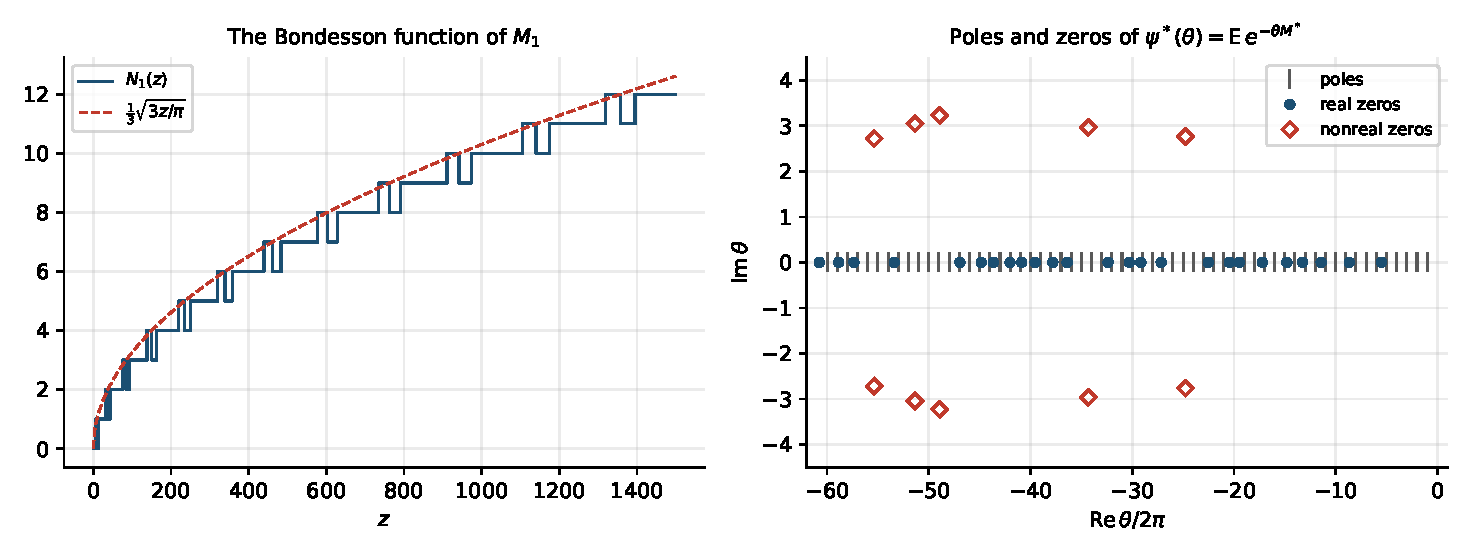
\includegraphics[width=\textwidth]{fig/maxexp_laws.pdf}
\caption{Left: the Bondesson function $N_1$ of $M_1$, nonnegative, with its asymptote $\frac13\sqrt{3z/\pi}$; each drop is a zero of the transform at $-b_{6k}$. Right: the poles $-2\pi m$, $m\le60$, and the zeros of $\psi^*(\theta)=\E e^{-\theta M^*}$: the $25$ real zeros above $-2\pi\times61$, one in each gap with $\tau(m+1)\tau(m+2)>0$, and the five pairs of nonreal zeros, the only ones with $|\re\theta|\le2\pi\times60.5$ and $|\im\theta|\le100$. Drawn by \texttt{maxexp\_figs.py} from \texttt{maxexp\_psizeros.json}.}
\label{fig:maxexp:laws}
\end{figure}

For the clock the relaxation from GGC to BO gains nothing. If its L\'evy density $W(t)/t$ were completely monotone, equal to $\int e^{-zt}\mu(dz)$ with $\mu\ge0$, then the formula $(G'/G)(u)=\int_0^\infty e^{-ut}W(t)\,dt$ of Section~\ref{ch:clock} would give $(G'/G)(u)=\int\mu(dz)(u+z)^{-2}$, holomorphic on $\cut$. But $G'/G$ has a pole at every zero $-a_k=(\rho_k-\frac12)^2$ of $G$, and this point lies in $(-\infty,0]$ only when $\rho_k$ is on the critical line. So the clock is in BO if and only if RH holds (Table~\ref{tab:ch3:hierarchy}). The signed Thorin measures of the max laws come from zeros of their Laplace transforms, and the transform $1/G$ of the clock has none. The two laws of this section show the two ways out of the Thorin class: $M_1$ leaves it through real zeros, each preceded by its own pole, and stays in BO, while $M^*$ leaves BO too, through zeros off the real axis, the way a zero of $\xi$ off the critical line would take the clock out of both classes.

Table~\ref{tab:maxexp:checks} collects the checks of this section, in the form of the table of the first author's note, recomputed.

\begin{table}[htbp]
\centering\small
\begin{tabular}{llp{0.24\textwidth}}
\toprule
quantity & max representation & check\\
\midrule
$L(\frac{17}2,\Delta)=\E\,Q(14,2\pi M^*)$ & $0.998583063162746176492$ & \raggedright Hecke: same; series to $n=400$: $18$ digits\tabularnewline
$L(\frac{29}2,\Delta)=\E\,Q(20,2\pi M^*)$ & $0.999977182799369841175$ & \raggedright series: same\tabularnewline
$\xi(\frac12,\Delta)$, symmetric form & $0.00154487936039502721$ & \raggedright \eqref{eq:ch16:max}, Hecke: same\tabularnewline
\eqref{eq:maxexp:fe}, $k=1$ & $0.00595896498957823785$ & \raggedright $k=11$: same\tabularnewline
\eqref{eq:maxexp:fe}, $k=5$ & $0.00163398603484069935$ & \raggedright $k=7$: same\tabularnewline
$L(\frac12,\Delta)=\Pr(N(2\pi M^*)\le5)$ & $0.792122838646030569$ & \raggedright Hecke: same\tabularnewline
first zero of $\xi(\frac12+i\theta,\Delta)$ & $9.2223793999211025222$ & \raggedright Hecke: same; \cite{LMFDB}: $9.222379$\tabularnewline
first zero of $K_{i\theta}(2\pi)$ & $9.768770083509977867$ & \raggedright moved to $9.2224$ by $H$\tabularnewline
$L(1,\chi_{12})$, $\operatorname{erfc}$ form & $0.760345996300946347531$ & \raggedright $\log(2+\sqrt3)/\sqrt3$: same\tabularnewline
$L(1,E)=\E e^{-2\pi M_{11}}$ & $0.253841860855910684338$ & \raggedright series of root number one: same\tabularnewline
$\E K$ from $\vartheta_4$ & $0.868731160636159141830$ & \raggedright $\sqrt{\pi/2}\,\log2$: same\tabularnewline
$\E e^{-2M_1}$, quadrature & $0.694250350153875231803$ & \raggedright closed form: same\tabularnewline
$\E e^{-3M_4}$, quadrature & $0.285645278943791835551$ & \raggedright $\sqrt{3\pi}/\sinh\sqrt{3\pi}$: same\tabularnewline
zeros of $\psi_1$ & $-b_{6k}=-\frac{36k^2-1}{12}\pi$ & \raggedright closed form vanishes at $k=1,2$\tabularnewline
$-\log|\E e^{5iM_1}|^2$ & $0.40295014525377167405$ & \raggedright Thorin sum: same; $\int N_1$: $18$ digits\tabularnewline
$-\psi_1'(2)/\psi_1(2)$ & $0.16796840787856222484$ & \raggedright Thorin sum: same; $\int N_1$: to $2\times10^{-15}$\tabularnewline
$-\log\psi_1(2)$ & $0.36492264843255339528$ & \raggedright L\'evy integral: same\tabularnewline
first zero of $\psi^*$ & $-2\pi\times5.48830041253$ & \raggedright certified; the only zero for $|\re\theta|\le15\pi$, $|\im\theta|\le60$ (computed)\tabularnewline
first nonreal zero of $\psi^*$ & $-155.59408228\pm2.76311889\,i$ & \raggedright certified\tabularnewline
\bottomrule
\end{tabular}
\caption[Checks of the max representation and of the laws of $M_1$ and $M^*$]{Checks of Section~\ref{sec:ch16:max}, by \texttt{maxlaw.py}, \texttt{maxexp\_checks.py} and \texttt{maxexp\_psizeros.py}, with $\psi_1(\theta)=\E e^{-\theta M_1}$; ``same'' means agreement to all digits shown. The first six rows are computed from the product for $F$ and the density \eqref{eq:maxexp:density}, independently of the Dirichlet series; the zeros of $\psi^*$ are those of Proposition~\ref{prop:maxexp:psizeros}.}
\label{tab:maxexp:checks}
\end{table}

\subsection{The de Bruijn Newman flow for \texorpdfstring{$\Delta$}{Delta}}\label{sec:ch16:dbn}

The flow of Section~\ref{ch:dbn} needs only an even kernel that decays faster than any Gaussian, so it applies to $K_\Delta$:
\[
H^\Delta_t(\theta)=\int_0^\infty e^{tu^2}K_\Delta(u)\cos(\theta u)\,du,\qquad 2H^\Delta_0(\theta)=\xi\big(\tfrac12+i\theta,\Delta\big).
\]
In the variable $\theta$ the times of Section~\ref{ch:dbn}, whose variable is $z=2\theta$, are divided by four, and the isolated pair estimate for two zeros at distance $D$ is $-D^2/8$. The zeros of $H^\Delta_0$ lie in the strip $|\im\theta|<\frac12$, so by de Bruijn's theorem \cite{deBruijn} every zero of $H^\Delta_t$ is real for $t\ge\frac18$; for $\zeta$ the same strip gives de Bruijn's bound $\Lambda\le\frac12$ in the times of Section~\ref{ch:dbn}. Dobner's theorem for the extended Selberg class \cite{Dobner21} gives the other side: $\Delta$ has a de Bruijn Newman constant $\Lambda_\Delta$, and $H^\Delta_t$ has nonreal zeros for every $t<0$. So $0\le\Lambda_\Delta\le\frac18$, and GRH for $\Delta$ is the statement $\Lambda_\Delta=0$.

On the critical line the kernel is a probability density up to normalisation, as the eta kernel is in Section~\ref{sec:ch16:eta}: if $V$ has the density $K_\Delta(v)/\xi(\frac12,\Delta)$ on $\R$, then $\E e^{i\theta V}=\xi(\frac12+i\theta,\Delta)/\xi(\frac12,\Delta)$, and GRH for $\Delta$ is the statement that this characteristic function has only real zeros. In the language of Section~\ref{sec:ch16:max}, $e^V$ has the density proportional to $y^5\Delta(iy)=y^5e^{-2\pi y}F(y)$, so $V$ is the logarithm of $G_6/2\pi$ conditioned on $G_6/2\pi\ge M^*$, with $G_6$ a gamma variable of shape $6$ independent of $M^*$; its law is symmetric by the self duality \eqref{eq:maxexp:dual}, with no symmetrisation. The variable $V$ is not infinitely divisible, nor even quasi infinitely divisible, because its characteristic function vanishes at $\theta=9.2223793999$; this is the argument of Proposition~\ref{sb:prop:qid}(1) for the P\'olya variable. Since $1-\cos x=2\sin^2(x/2)$ and $K_\Delta$ is even,
\[
\xi\big(\tfrac12,\Delta\big)-\xi\big(\tfrac12+i\theta,\Delta\big)=4\int_0^\infty K_\Delta(v)\sin^2\Big(\frac{\theta v}2\Big)dv,
\]
so the zeros on the critical line are the solutions of $\E[2\sin^2(\theta V/2)]=1$. At the level of logarithms, the factorisation $\xi(s,\Delta)=(2\pi)^{-s-11/2}\Gamma(s+\frac{11}2)L(s,\Delta)$ splits $\log|\xi(\frac12+i\theta,\Delta)/\xi(\frac12,\Delta)|^2$ into $\log|\Gamma(6+i\theta)/\Gamma(6)|^2$ and $\log|L(\frac12+i\theta,\Delta)/L(\frac12,\Delta)|^2$. The first has the positive sine squared form given by Binet's formula,
\[
\log\Big|\frac{\Gamma(6+i\theta)}{\Gamma(6)}\Big|^2=-\int_0^\infty4\sin^2\Big(\frac{\theta u}2\Big)\frac{e^{-6u}}{u(1-e^{-u})}\,du,
\]
the L\'evy Khintchine form of the infinitely divisible variable $\log G_6$, and the second carries every zero. To the right of the critical strip the second has a sine squared form too: for $\sigma>1$, expanding $\log L(s,f)=\sum_{n\ge2}\Lambda_f(n)n^{-s}/\log n$ gives
\[
\log\Big|\frac{L(\sigma+i\theta,f)}{L(\sigma,f)}\Big|^2=-\sum_{n\ge2}\frac{4\Lambda_f(n)}{n^\sigma\log n}\sin^2\Big(\frac{\theta\log n}2\Big),
\]
for $f=\chi_{12}$ and $\Delta$, and for $\zeta$ with $\Lambda$ in place of $\Lambda_f$. Since $\int_\sigma^\infty n^{-\alpha}d\alpha=n^{-\sigma}/\log n$, the right side is minus twice the integral of the prime piece of the decomposition of Section~\ref{sec:ch16:sin2} over the basepoints $\alpha>\sigma$. For $\zeta$ the weights are positive, which is the infinite divisibility of $\log$ of the zeta distribution (Section~\ref{rz:sec:strip}). For $\Delta$ they are $8\cos(k\vartheta_p)/(kp^{k\sigma})$ at $n=p^k$, where $\alpha_p=e^{i\vartheta_p}$, $0\le\vartheta_p\le\pi$, and they take both signs. The Sato Tate law for $\Delta$, proved by Barnet-Lamb, Geraghty, Harris and Taylor \cite{BLGHT11}, makes the angles $\vartheta_p$ equidistributed for the measure $\frac2\pi\sin^2\vartheta\,d\vartheta$ on $[0,\pi]$, under which $\cos k\vartheta<0$ with probability $\frac12$ for $k\ne2$ and $\frac12+\frac1\pi$ for $k=2$. So even where the Euler product converges absolutely the sine squared form of $\log|L(\sigma+i\theta,\Delta)|$ has a signed measure, and on the critical line the series diverges: positivity lives in the kernel and in the gamma factor, not in the arithmetic factor.

The kernel factors as $K_\Delta(u)=e^{-2\pi\cosh u}H(u)$, with $H(u)=\sqrt{F(e^u)F(e^{-u})}$ because $K_\Delta(u)^2=K_\Delta(u)K_\Delta(-u)$, and $\log H(u)=-12\sum_m\frac{\sigma(m)}m(e^{-2\pi me^u}+e^{-2\pi me^{-u}})$. The expansion comes from $-\log F(y)=24\sum_{m\ge1}\frac{\sigma(m)}me^{-2\pi my}$, so $-\log F$ is completely monotone, the Laplace transform of the positive measure with mass $24\sigma(m)/m$ at each point $2\pi m$; for $\eta$ the masses are $\sigma(m)/m$, and every maximum of independent exponential variables has this property, since $-\log(1-e^{-\lambda y})=\sum_ke^{-k\lambda y}/k$. The transform $K_{i\theta}(2\pi)$ of P\'olya's factor has only real zeros \cite{Polya}, the first at $\theta=9.768770083509977867$ (\texttt{maxlaw.py}), and the multiplier $H$ moves it to $9.2223793999$. P\'olya's theorem on universal factors \cite[p.~197]{deBruijn}, which covers the Gaussian multiplier $e^{tu^2}$ of the flow for $t>0$, does not apply to $H$, which is bounded by one and supplies half of the doubly exponential decay of $K_\Delta$. The positivity of the measure of $-\log F$ is automatic and does not by itself decide where the zeros are; whether some multiplier of the same form moves zeros off the line is the following question, and any answer must account for $\Delta$, $\chi_{12}$ and the conductor $11$ curve, whose kernels have this form. Figure~\ref{fig:maxexp:kernels} shows the two kernels and $\log H$.

\begin{question}\label{q:maxexp:mult}
For which $a>0$, $c_m\ge0$ and $\beta_m>0$ does the Fourier transform of $e^{-a\cosh u}\exp\big(-\sum_mc_m(e^{-\beta_me^u}+e^{-\beta_me^{-u}})\big)$ have only real zeros?
\end{question}

\begin{figure}[htbp]
\centering
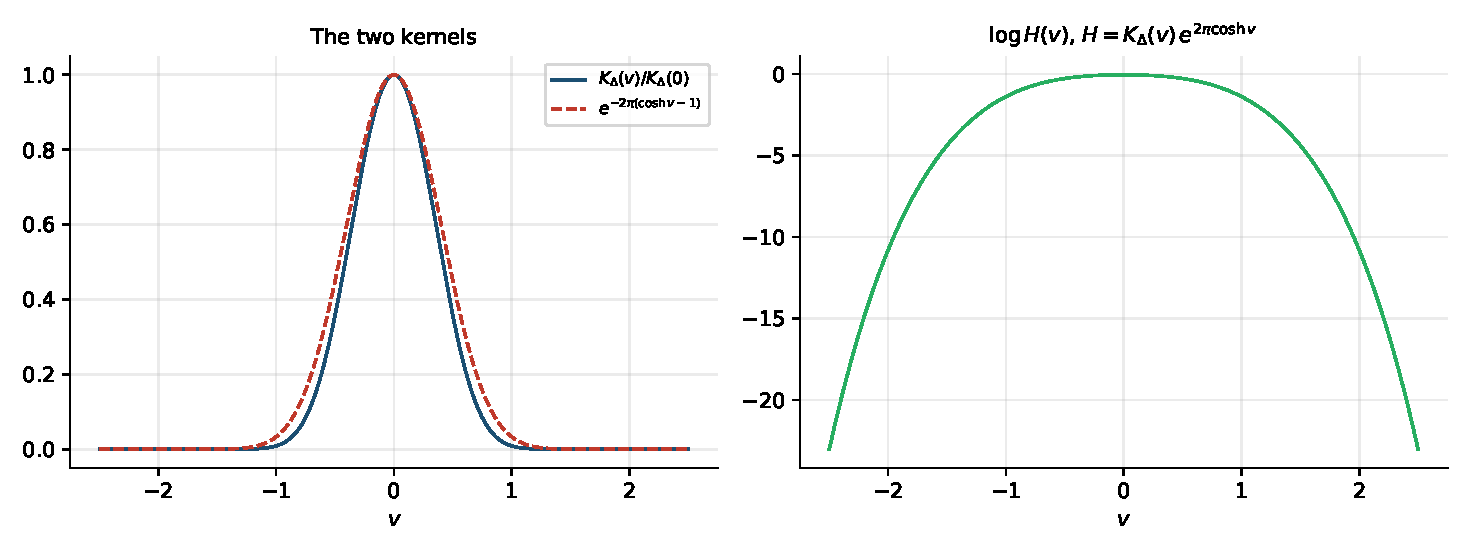
\includegraphics[width=\textwidth]{fig/maxexp_kernels.pdf}
\caption{Left: the kernel $K_\Delta(v)=e^{6v}\Delta(ie^v)$ and P\'olya's kernel $e^{-2\pi\cosh v}$, each divided by its value at $0$. Right: the logarithm of the multiplier $H(v)=\sqrt{F(e^v)F(e^{-v})}$; $-\log H$ expands with the positive coefficients $12\sigma(m)/m$. Drawn by \texttt{maxexp\_figs.py}.}
\label{fig:maxexp:kernels}
\end{figure}

The kernel $K_\Delta$ is strictly log concave, as the first author's note \cite{P26thor} shows, and the product formula gives the best constant. For $c>0$, $\log(1-e^{-ce^u})$ is the logarithm of the distribution function of $\log E$, with $E$ exponential of rate $c$, and it is strictly concave in $u$: with $x=ce^u$ its second derivative is $x(e^x-1-xe^x)/(e^x-1)^2<0$. So $\log F(e^u)$, a sum of such terms, is strictly concave (in the language of Section~\ref{sec:ch16:max}, $\log M^*$ has a log concave distribution function), and since $\log K_\Delta(u)=6u-2\pi e^u+\log F(e^u)$ and $K_\Delta$ is even,
\[
-\big(\log K_\Delta\big)''(u)>2\pi e^{|u|},\qquad u\in\R,
\]
where the ratio of the two sides tends to $1$ as $|u|\to\infty$. The multiplier $H$ is log concave as well, since $\log H(u)=\frac12\big(\log F(e^u)+\log F(e^{-u})\big)$. In the same way $\log K(u)=\log2+\frac u2-\frac\pi{12}e^{2u}+\log F_1(e^{2u})$ gives $-(\log K)''(u)>\frac\pi3e^{2|u|}$ for the kernel of Section~\ref{sec:ch16:eta}. The P\'olya kernel $\Phi$ is log concave too \cite{CC13}, though it is not a product of this kind. Log concavity alone does not put the zeros of a transform on a line, or in any strip. The function $(1-|u|)_+^2$ is log concave, and its transform $4(\theta-\sin\theta)/\theta^3$ vanishes at the nonzero roots of $\sin\theta=\theta$, which are nonreal, the first at $7.4977+2.7687i$, with imaginary parts that grow like $\log|\theta|$. Its convolution with $e^{-\cosh u}$ is even, positive, entire and log concave \cite{SW14}, and decays doubly exponentially, like $K_\Delta$; its transform $8(\theta-\sin\theta)K_{i\theta}(1)/\theta^3$ has the same nonreal zeros.

In the language of Section~\ref{sec:ch16:max} the flow is a family of Gaussian tilts: for every real $t$, $e^{tv^2}K_\Delta(v)$ is integrable, because $K_\Delta$ decays doubly exponentially, so after normalisation it is the density of the law of $V$ tilted by $e^{tV^2}$, and $H^\Delta_t(\theta)/H^\Delta_t(0)$ is its characteristic function. The question $\Lambda_\Delta=0$ asks whether the smallest tilt whose characteristic function has only real zeros is $t=0$.

The script \texttt{dbn\_delta.py} computes $H^\Delta_t$ by Gauss Legendre quadrature on $[0,4]$, beyond which $K_\Delta<10^{-130}$, with $8$ panels of $96$ nodes at $40$ digits; at $t=0$ it agrees with $192$ nodes per panel and with Hecke's formula to a relative $4\times10^{-41}$ at $\theta=0$ and $5\times10^{-16}$ at $\theta=50$. The $21$ zeros below height $52$, from $9.2224$ to $51.1566$, stay real for $t=0.05,0.1,\dots,0.5$ and all move down. Backward in time each pair of neighbours is followed through the critical point of $H^\Delta_t$ between them until the critical value changes sign, and each such event is tested by direct sign counts: a collision at $(t_*,\theta_*)$ leaves two sign changes on $[\theta_*-1.2,\theta_*+1.2]$ at $t_*+0.005$ and none at $t_*-0.005$, and the colliding pair is identified by the number of sign changes below $\theta_*-1.2$, since real zeros keep their order. Table~\ref{tab:ch16:coll} lists the seven collisions. The numbers of sign changes on $(0.5,52]$ at eleven values of $t$ from $0$ to $-1.5$ fall by two at each collision and once by one, between $t=-0.2$ and $-0.3$, where the highest zero, followed back from $51.1566$, passes $52$ at $t\approx-0.29$.

\begin{table}[htbp]
\centering\small
\begin{tabular}{cccc}
\toprule
pair at $t=0$ & $-D^2/8$ & $t_*$ & $\theta_*$\\
\midrule
$48.3591$, $49.2761$ & $-0.1051$ & $-0.12622$ & $49.18$\\
$36.7415$, $37.7539$ & $-0.1281$ & $-0.15864$ & $37.60$\\
$45.0401$, $46.1973$ & $-0.1674$ & $-0.24305$ & $46.19$\\
$25.2746$, $26.8044$ & $-0.2925$ & $-0.40713$ & $27.26$\\
$40.2190$, $41.7305$ & $-0.2856$ & $-0.48271$ & $42.49$\\
$31.1782$, $32.7749$ & $-0.3187$ & $-0.48637$ & $33.30$\\
$17.4428$, $19.6565$ & $-0.6126$ & $-0.98116$ & $21.09$\\
\bottomrule
\end{tabular}
\caption{The collisions of zeros of $H^\Delta_t$ below height $52$, in the order in which they occur as $t$ decreases: the pair at $t=0$, the isolated pair estimate with $D$ the gap of the pair, and the time $t_*$ and height $\theta_*$ of the collision, computed by \texttt{dbn\_delta.py}.}
\label{tab:ch16:coll}
\end{table}

The script \texttt{maxexp\_flow.py} recomputes the table independently, at $70$ digits for the kernel and with a different tracking: it evaluates $H^\Delta_t$ at once on the grid $\theta=0.5,0.52,\dots,52$, with the cosines kept in fixed point by their three term recurrence, for $t=0.5,0.49,\dots,-1.1$, locates the zeros by inverse interpolation, and refines each fall of the count by two to the time at which the critical value between the closest pair changes sign. It finds the same seven collisions, with the same $t_*$ and $\theta_*$ to all digits of the table (for instance $t_*=-0.4071263919$, $\theta_*=27.257965$), and the highest zero passing $52$ between $t=-0.29$ and $-0.30$. Figure~\ref{fig:maxexp:flow} shows the trajectories.

\begin{figure}[htbp]
\centering
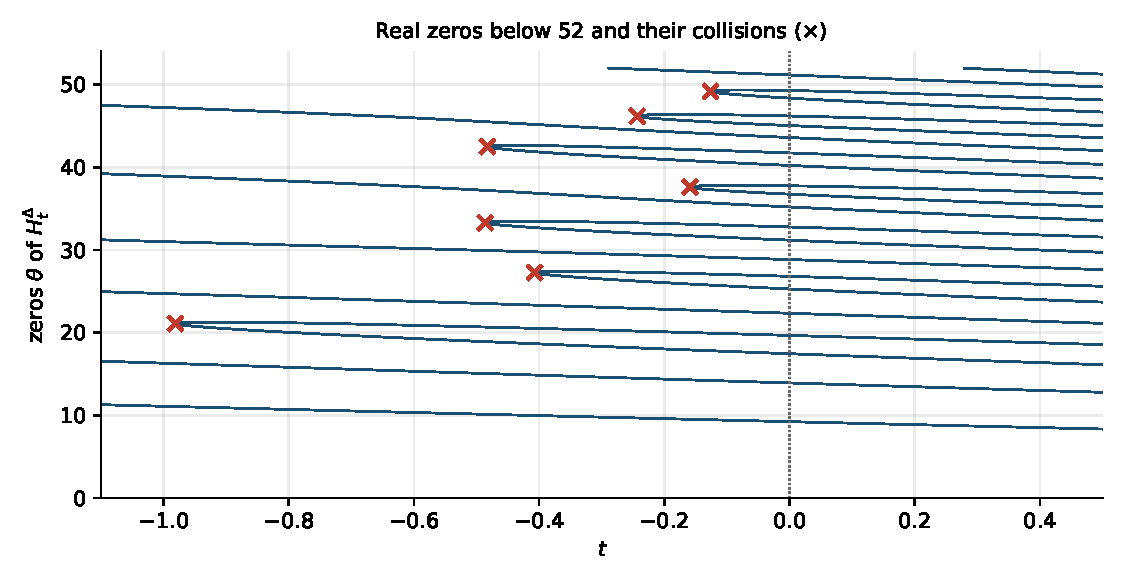
\includegraphics[width=0.8\textwidth]{fig/maxexp_flow.pdf}
\caption{The real zeros of $H^\Delta_t$ below height $52$ for $-1.1\le t\le0.5$, and the seven collisions of Table~\ref{tab:ch16:coll}; all zeros move down as $t$ grows. Drawn by \texttt{maxexp\_figs.py} from \texttt{maxexp\_flow.json}.}
\label{fig:maxexp:flow}
\end{figure}

The low zeros of $\Delta$ are robust: below height $33$, the window of the first author's note, the first pair to leave the line, $(25.27,26.80)$, does so only at $t=-0.407$. Collisions do not come in order of height, however. The pairs near $37.6$ and $49.2$ collide at $-0.159$ and $-0.126$, and under GRH for $\Delta$ Dobner's theorem forces collisions in every interval $(t,0)$, higher up; so no window of heights decides whether $\Lambda_\Delta=0$ (Dobner's theorem already gives $\Lambda_\Delta\ge0$), and what a computation can show is how fast the collision times approach $0$ with height. The neighbours delay every collision beyond the isolated pair estimate, by factors from $1.20$ to $1.69$. In the variable $\theta$ the closest pair of $\zeta$ below height $200$ collides at $-0.072$, and Lehmer's pair near height $7005$ at $-1.8\times10^{-4}$ (Section~\ref{sec:ch21:collisions}).

\subsection{A P\'olya kernel for imaginary quadratic fields}\label{sec:sqfree:quad}

Section~\ref{sec:ch16:eta} left the positivity of the kernels of odd characters to be checked case by case. For the Dedekind zeta function of an imaginary quadratic field the kernel comes from a simple theta series, its positivity reduces to a finite interval, and it fails for a whole residue class of discriminants, together with the kernel of the odd character. This subsection follows the last part of the first author's note on the squarefree series \cite{P26sqf}; the constants of number fields, which these kernels turn into tilted means, are in Section~\ref{sec:sqfree:nf} of Chapter~\ref{chap:strip}.

Let $d<0$ be a fundamental discriminant, $K=\mathbb Q(\sqrt d)$, $\chi_d$ the Kronecker symbol of $d$, a real primitive odd character modulo $|d|$, $h$ the class number of $K$ and $w$ the number of its roots of unity. Then $\zeta_K(s)=\zeta(s)L(s,\chi_d)=\sum_{n\ge1}a_nn^{-s}$, where $a_n=\sum_{m\mid n}\chi_d(m)\ge0$ is the number of ideals of norm $n$, and we put
\[
\Lambda_K(s)=\Big(\frac{\sqrt{|d|}}{2\pi}\Big)^s\Gamma(s)\,\zeta_K(s),\qquad \xi_K(s)=2s(s-1)\Lambda_K(s),
\]
the function $\xi_K$ of Section~\ref{sec:sqfree:nf} with $r_1=0$ and $r_2=1$. The duplication formula gives $\xi_K(s)=\frac2{\sqrt{|d|}}\,\xi(s)\,\xi(s,\chi_d)$, with $\xi(s,\chi_d)=(|d|/\pi)^{(s+1)/2}\Gamma(\frac{s+1}2)L(s,\chi_d)$ the completed function of Section~\ref{sec:ch16:eta}, so $\xi_K(s)=\xi_K(1-s)$ because the root number of $\chi_d$ is one. Hence $\Lambda_K(s)=\Lambda_K(1-s)$, and $\Lambda_K$ is meromorphic with simple poles at $s=1$ and $s=0$ only, with residues $h/w$ and $-h/w$, by the class number formula $L(1,\chi_d)=2\pi h/(w\sqrt{|d|})$ and the symmetry. Let
\[
\vartheta_K(x)=\sum_{n\ge1}a_n\,e^{-2\pi nx/\sqrt{|d|}},\qquad \Psi(y)=y(y-2)\,e^{-y},\qquad H_K(x)=\big(x^2\vartheta_K'(x)\big)',
\]
and $\Phi_K(u)=2e^{u/2}H_K(e^u)$.

\begin{theorem}\label{thm:sqfree:kernelK}
\textup{(i)} $\vartheta_K(1/x)=x\,\vartheta_K(x)+\frac hw\,(x-1)$ for $x>0$.

\textup{(ii)} $H_K(x)=\sum_{n\ge1}a_n\Psi(2\pi nx/\sqrt{|d|})$ and $H_K(1/x)=x\,H_K(x)$. The kernel $\Phi_K$ is even, analytic in the strip $|\im u|<\frac\pi2$, and decays doubly exponentially.

\textup{(iii)} $\xi_K(\frac12+s)=\int_{\R}\Phi_K(u)\,e^{su}\,du$ for every $s\in\C$; in particular $\xi_K(\frac12+i\theta)=\int_{\R}\Phi_K(u)\cos(\theta u)\,du$.

\textup{(iv)} $\Phi_K>0$ on $\R$ if and only if $H_K>0$ on $[1,\sqrt{|d|}/\pi]$. In particular $\Phi_K>0$ when $|d|<\pi^2$, that is for $d=-3,-4,-7,-8$.

\textup{(v)} If $\Phi_K>0$, then $\zeta_K(\frac12)<0$ and $L(\frac12,\chi_d)>0$. In particular $L(\frac12,\chi_d)>0$ for $d=-3,-4,-7,-8$.
\end{theorem}

\begin{proof}
(i) For $c>1$, Mellin inversion of $\int_0^\infty e^{-2\pi nx/\sqrt{|d|}}x^{s-1}dx=\Gamma(s)\big(\sqrt{|d|}/2\pi n\big)^s$ gives $\vartheta_K(x)=\frac1{2\pi i}\int_{(c)}\Lambda_K(s)x^{-s}ds$. Move the line of integration to $\re s=1-c$, which the exponential decay of $\Gamma$ and the polynomial growth of $\zeta_K$ on vertical strips allow; the residues at $s=1$ and $s=0$ are $\frac hwx^{-1}$ and $-\frac hw$. On the new line substitute $s\mapsto1-s$ and use $\Lambda_K(1-s)=\Lambda_K(s)$: the integral becomes $x^{-1}\vartheta_K(1/x)$. So $\vartheta_K(x)=\frac hw(x^{-1}-1)+x^{-1}\vartheta_K(1/x)$, which is (i).

(ii) Termwise, $\big(x^2\frac d{dx}e^{-\kappa x}\big)'=(\kappa^2x^2-2\kappa x)e^{-\kappa x}=\Psi(\kappa x)$. Differentiating (i) gives $\vartheta_K'(1/x)=-x^2\big(\vartheta_K(x)+x\vartheta_K'(x)+\frac hw\big)$, so $g(x)=x^2\vartheta_K'(x)$ satisfies $g(1/x)=-\big(\vartheta_K(x)+x\vartheta_K'(x)+\frac hw\big)$, and differentiating again gives $g'(1/x)=x^2\big(2\vartheta_K'(x)+x\vartheta_K''(x)\big)=x\,g'(x)$, that is $H_K(1/x)=xH_K(x)$. Then $\Phi_K(-u)=2e^{-u/2}H_K(e^{-u})=2e^{u/2}H_K(e^u)=\Phi_K(u)$. Since $a_n\le n$, the series for $H_K(e^u)$ converges locally uniformly where $\re e^u>0$, that is for $|\im u|<\frac\pi2$; and $\Phi_K(u)=O\big(e^{5u/2}\exp(-2\pi e^u/\sqrt{|d|})\big)$ as $u\to\infty$, and likewise as $u\to-\infty$ by evenness.

(iii) By (i), $x\vartheta_K(x)\to\frac hw$ and $x^2\vartheta_K'(x)\to-\frac hw$ as $x\to0$, while $\vartheta_K$ and $\vartheta_K'$ decay exponentially at infinity. For $\re z>1$ two integrations by parts, whose boundary terms vanish, give $\int_0^\infty H_K(x)x^{z-1}dx=z(z-1)\int_0^\infty\vartheta_K(x)x^{z-1}dx=z(z-1)\Lambda_K(z)$. With $x=e^u$ and $z=\frac12+s$, $\int_{\R}\Phi_K(u)e^{su}du=2\int_0^\infty H_K(x)x^{z-1}dx=\xi_K(z)$. Both sides are entire in $s$, the left by (ii), so the identity holds for every $s$.

(iv) By (ii), $\Phi_K>0$ exactly when $H_K>0$ on $(0,\infty)$, and by the symmetry exactly when $H_K>0$ on $[1,\infty)$. For $x\ge\sqrt{|d|}/\pi$ every argument $2\pi nx/\sqrt{|d|}$ is at least $2n\ge2$, where $\Psi\ge0$, and the term $n=4$ is positive, since $a_4=1+\chi_d(2)+\chi_d(2)^2\ge1$; so $H_K>0$ there. If $|d|<\pi^2$ the interval $[1,\sqrt{|d|}/\pi]$ is empty.

(v) By (iii), $\xi_K(\frac12)=\int_{\R}\Phi_K>0$, while
\[
\xi_K\big(\tfrac12\big)=-\tfrac12\Lambda_K\big(\tfrac12\big)=-\tfrac12\big(\sqrt{|d|}/2\pi\big)^{1/2}\sqrt\pi\,\zeta_K\big(\tfrac12\big).
\]
So $\zeta_K(\frac12)<0$, and $L(\frac12,\chi_d)=\zeta_K(\frac12)/\zeta(\frac12)>0$ because $\zeta(\frac12)<0$.
\end{proof}

When $\Phi_K>0$, the normalised kernel $\Phi_K/\xi_K(\frac12)$ is the density of a symmetric variable $X_K$ with $\E e^{sX_K}=\xi_K(\frac12+s)/\xi_K(\frac12)$, the P\'olya variable of $K$, and its tilts $V_{K,\alpha}$, with $\E e^{sV_{K,\alpha}}=\xi_K(\alpha+s)/\xi_K(\alpha)$, have the means $\frac{\xi_K'}{\xi_K}(\alpha)$. The zero part of the constant $C_K$ of Theorem~\ref{thm:sqfree:constK} is then $\E V_{K,1}-2\,\E V_{K,2}$, as over $\mathbb Q$ in Theorem~\ref{thm:sqfree:const}; by (iv) this applies to the Gaussian field $d=-4$ of Section~\ref{sec:sqfree:nf}. If moreover the Riemann hypothesis holds for $\zeta_K$, that is RH for $\zeta$ and for $L(s,\chi_d)$, then $1/\E\cosh(\sqrt u\,X_K)=\xi_K(\frac12)/\xi_K(\frac12+\sqrt u)$ is the Laplace transform of a GGC, the clock of $K$ (Proposition~\ref{prop:sqfree:thorinK}).

The kernel $\Phi_K$ is tied to the kernel of $\chi_d$ in Section~\ref{sec:ch16:eta},
\[
K_{\chi_d}(u)=2e^{3u/2}\sum_{n\ge1}n\chi_d(n)\,e^{-\pi n^2e^{2u}/|d|},\qquad \xi\big(\tfrac12+s,\chi_d\big)=\int_{\R}K_{\chi_d}(u)\,e^{su}\,du .
\]
Since the two sided Laplace transform turns convolution into multiplication, the identity $\xi_K=\frac2{\sqrt{|d|}}\xi\cdot\xi(\cdot,\chi_d)$ and (iii) give $\Phi_K=\frac2{\sqrt{|d|}}\,\Phi*K_{\chi_d}$, with $\Phi$ the P\'olya kernel \eqref{eq:ch2:Phi}. As $\Phi>0$, the kernel $\Phi_K$ is positive whenever $K_{\chi_d}$ is, and if $\Phi_K$ takes a negative value, so does $K_{\chi_d}$. For $d=-4$ Jacobi's identity $\sum_{n\ge0}(-1)^n(2n+1)q^{(2n+1)^2/8}=q^{1/8}\prod_{n\ge1}(1-q^n)^3$ gives $K_{\chi_{-4}}(u)=2e^{3u/2}\eta(ie^{2u})^3>0$, positive by the product formula as the kernel of $\chi_{12}$ is.

The script \texttt{sqfree\_quadratic.py} checks the theorem at $30$ digits. For $d=-4$, where $h/w=\frac14$, the trapezoid rule with step $1/200$ gives $\int\Phi_K(u)\cos(\theta u)\,du=0.48753311500024448536$ at $\theta=0$ and $0.25376667901239784985$ at $\theta=2.5$, equal to $\xi_K(\frac12+i\theta)$ in every digit shown; (i) holds at $x=1.5$ and $2$, and the evenness of $\Phi_K$ at $u=0.3$ and $0.6$, within $10^{-31}$; and $H_K(1/x)=xH_K(x)$ holds at $x=1.25$ within $3\times10^{-31}$ for $d=-23$ and $d=-163$, where $H_K(1.25)=0.55669258$ and $-0.28242077$. The values $\zeta_K(\frac12)=-0.70223711$, $-0.97506623$, $-1.6744215$ and $-1.6070054$ for $d=-3,-4,-7,-8$ are negative, as (v) requires.

Since $\int_0^\infty\Psi(y)\,dy=0$, the value $H_K(1)=\sum_na_n\Psi(2\pi n/\sqrt{|d|})$ is a Riemann sum, with step $2\pi/\sqrt{|d|}$ and weights $a_n$ of mean value $L(1,\chi_d)$, of a function with integral zero. For large $|d|$ it is small compared with the sum of the absolute values of its terms, and its sign, like the sign of $H_K$ elsewhere on $[1,\sqrt{|d|}/\pi]$, depends strongly on the first few weights: $\Psi$ is negative on $(0,2)$ and positive beyond, and the weights $a_2=1+\chi_d(2)$ and $a_3=1+\chi_d(3)$ vanish when $2$ and $3$ are inert in $K$. The next theorem makes this precise at the point where the term $n=1$ sits in the negative part of $\Psi$ and the terms $n=2$ and $3$, which would compensate it, vanish.

\begin{theorem}\label{thm:sqfree:inert}
Let $d<0$ be a fundamental discriminant with $\chi_d(2)=\chi_d(3)=-1$, that is $d\equiv5\pmod{24}$. Then $H_K(x)<0$ at $x=1.42\sqrt{|d|}/2\pi$, so $\Phi_K$ takes negative values, and so does the kernel $K_{\chi_d}$. There are infinitely many such $d$, for instance $d=-p$ for every prime $p\equiv19\pmod{24}$.
\end{theorem}

\begin{proof}
For a fundamental discriminant $d<0$, $\chi_d(2)=-1$ exactly when $d\equiv5\pmod8$, and $\chi_d(3)=-1$ exactly when $d\equiv2\pmod3$; together they give $d\equiv5\pmod{24}$. The function $n\mapsto a_n$ is multiplicative, with $a_{p^k}=\frac12(1+(-1)^k)$ when $\chi_d(p)=-1$ and $a_{p^k}\le k+1$ for every $p$. Hence $a_1=1$, $a_2=a_3=0$ and $a_n\le a_n^*$, where $a_n^*=0$ unless $2$ and $3$ divide $n$ to even powers, and otherwise $a_n^*$ is the number of divisors of $n$ with its factors $2$ and $3$ removed. At $x=1.42\sqrt{|d|}/2\pi$ the $n$th argument of $\Psi$ in Theorem~\ref{thm:sqfree:kernelK}(ii) is $1.42n$, which exceeds $2$ for $n\ge2$, where $\Psi>0$. So
\begin{align*}
H_K(x)&\le\Psi(1.42)+\sum_{n\ge4}a_n^*\,\Psi(1.42n)\\
&=-0.19907566+0.13917904=-0.05989662<0,
\end{align*}
the sum taken to $n=2000$ and the rest bounded, with $a_n^*\le2\sqrt n$, by $10^{-1225}$ (\texttt{sqfree\_quadratic.py}). Then $\Phi_K(\log x)<0$, and $K_{\chi_d}$ takes negative values by the convolution identity above. If $p\equiv19\pmod{24}$ is prime, then $p\equiv3\pmod4$, so $-p$ is a fundamental discriminant, and $-p\equiv5\pmod{24}$; by Dirichlet's theorem there are infinitely many such primes.
\end{proof}

The bound is negative for every $y$ in $[1.107,1.879]$ on a grid of step $0.001$, with least value $-0.0598979$ at $y=1.418$, so the point $x=y\sqrt{|d|}/2\pi$ can be moved. By the symmetry $H_K(1/x)=xH_K(x)$ it does not matter whether $x$ lies in $[1,\sqrt{|d|}/\pi]$; for $d=-19$ it does not.

Table~\ref{tab:sqfree:named} shows the discriminants discussed in the first author's note. The four of class number one with $2$ and $3$ inert, $d=-19,-43,-67,-163$, take the least value of $H_K$ on $[1,\sqrt{|d|}/\pi]$ at the centre $x=1$, the two composite ones with $d\equiv5\pmod{24}$ inside the interval, and most of the positive kernels at its right end $\sqrt{|d|}/\pi$, where the term $n=1$ vanishes. All twenty values of $\zeta_K(\frac12)$ computed are negative, so $L(\frac12,\chi_d)>0$ for all of them whether or not the kernel is positive: Theorem~\ref{thm:sqfree:kernelK}(v) is a sufficient condition only.

\begin{table}[htbp]
\centering\small
\begin{tabular}{rrrcrrr}
\toprule
$d$ & $\chi_d(2)$ & $\chi_d(3)$ & $\Phi_K>0$ & least $H_K$ on $[1,\sqrt{|d|}/\pi]$ & at $x=$ & $\zeta_K(\frac12)$\\
\midrule
$-11$ & $-1$ & $1$ & yes & $0.14236$ & $1.0557$ & $-1.4480539$\\
$-15$ & $1$ & $0$ & yes & $0.40606$ & $1.2328$ & $-2.6973176$\\
$-20$ & $0$ & $1$ & yes & $0.287033$ & $1.4235$ & $-2.4529153$\\
$-23$ & $1$ & $1$ & yes & $0.4634$ & $1.5266$ & $-3.5856997$\\
$-24$ & $0$ & $0$ & yes & $0.225215$ & $1.2409$ & $-2.2955534$\\
$-31$ & $1$ & $-1$ & yes & $0.349008$ & $1.7723$ & $-3.2253855$\\
$-39$ & $1$ & $0$ & yes & $0.409694$ & $1.9878$ & $-4.0547932$\\
$-47$ & $1$ & $1$ & yes & $0.46368$ & $2.1822$ & $-4.8243519$\\
$-71$ & $1$ & $1$ & yes & $0.470667$ & $2.6821$ & $-5.9925928$\\
$-191$ & $1$ & $1$ & yes & $0.470667$ & $4.3991$ & $-8.1483722$\\
$-19$ & $-1$ & $-1$ & no & $-0.0596605$ & $1$ & $-1.1747378$\\
$-43$ & $-1$ & $-1$ & no & $-0.214707$ & $1$ & $-0.76635571$\\
$-67$ & $-1$ & $-1$ & no & $-0.251274$ & $1$ & $-0.54460945$\\
$-163$ & $-1$ & $-1$ & no & $-0.315818$ & $1$ & $-0.10008066$\\
$-427$ & $-1$ & $-1$ & no & $-0.181949$ & $3.1887$ & $-0.20993694$\\
$-1003$ & $-1$ & $-1$ & no & $-0.228309$ & $3.9479$ & $-0.64248774$\\
\bottomrule
\end{tabular}
\caption{The P\'olya kernel $\Phi_K$ of $K=\mathbb Q(\sqrt d)$ for the discriminants named in the first author's note: the characters at $2$ and $3$, the sign of the kernel, the least value of $H_K$ on $[1,\sqrt{|d|}/\pi]$, which decides it by Theorem~\ref{thm:sqfree:kernelK}(iv), with the point where it is attained, and $\zeta_K(\frac12)=\zeta(\frac12)L(\frac12,\chi_d)$. Computed by \texttt{sqfree\_quadratic.py}.}
\label{tab:sqfree:named}
\end{table}

The script also scans all $6079$ fundamental discriminants $-20000\le d<0$. It evaluates $H_K$ in double precision on $3000$ geometrically spaced points of $[1,\sqrt{|d|}/\pi]$, refines the least value by golden section search, and would recompute at $30$ digits any least value within $10^{-8}$ of zero; there is none. The kernel is positive for $2738$ of the discriminants. Table~\ref{tab:sqfree:quad} sorts them by the splitting of $2$ and $3$: the proportion of positive kernels falls as either prime goes from split to ramified to inert, and the class $d\equiv5\pmod{24}$ of Theorem~\ref{thm:sqfree:inert} has none among its $763$ members. By blocks of $2000$ in $|d|$ the proportion falls from $337/611$ for $|d|\le2000$ to between $0.41$ and $0.45$ in each of the five blocks above $10000$. Of the $3341$ negative kernels, $1546$ take the least value of $H_K$ on $[1,\sqrt{|d|}/\pi]$ at the centre $x=1$, and $1135$ the least value of $\Phi_K$ on $u\ge0$ at $u=0$.

\begin{table}[htbp]
\centering\small
\begin{tabular}{lccc}
\toprule
 & $\chi_d(3)=1$ & $\chi_d(3)=0$ & $\chi_d(3)=-1$\\
\midrule
$\chi_d(2)=1$ & $676/767$ & $334/507$ & $412/757$\\
$\chi_d(2)=0$ & $489/753$ & $178/514$ & $131/757$\\
$\chi_d(2)=-1$ & $397/761$ & $121/500$ & $0/763$\\
\bottomrule
\end{tabular}
\caption{Positive P\'olya kernels $\Phi_K$ among the $6079$ fundamental discriminants $-20000\le d<0$, by the splitting of $2$ and $3$ in $K=\mathbb Q(\sqrt d)$ ($\chi_d(p)=1$ split, $0$ ramified, $-1$ inert): the number of positive kernels over the number of discriminants in each class, $2738$ positive in all. The empty corner is Theorem~\ref{thm:sqfree:inert}. Computed by \texttt{sqfree\_quadratic.py}.}
\label{tab:sqfree:quad}
\end{table}

\begin{question}\label{q:sqfree:density}
Does the proportion of fundamental discriminants $-X\le d<0$ with $\Phi_K>0$ tend to a limit as $X\to\infty$, and is the limit positive? Is $\Phi_K$ positive for infinitely many $d$, for instance among the $d$ in which $2$ and $3$ split, where the proportion up to $20000$ is $676/767$?
\end{question}

\begin{question}\label{q:sqfree:realquad}
For real quadratic fields and for fields of higher degree the gamma factor $\Gamma_{\mathbb R}(s)^{r_1}\Gamma_{\mathbb C}(s)^{r_2}$ replaces the exponentials in $\vartheta_K$ by other kernels, for $\Gamma_{\mathbb R}(s)^2$ a Bessel function $K_0$. Is there a criterion for the positivity of the P\'olya kernel of $\xi_K$ as simple as Theorem~\ref{thm:sqfree:kernelK}(iv)?
\end{question}

\subsection{The Dirichlet beta function and the eta cube kernel}\label{sec:dbeta:beta}

The $L$ function of the odd character $\chi_4$ modulo $4$, with $\chi_4(n)=1$ for $n\equiv1$, $-1$ for $n\equiv3\pmod4$ and $0$ for even $n$,
\[
L(s,\chi_4)=\sum_{n\ge0}\frac{(-1)^n}{(2n+1)^s}=\prod_p\big(1-\chi_4(p)p^{-s}\big)^{-1},\qquad\re s>1,
\]
is the Dirichlet beta function, with $L(1,\chi_4)=\frac\pi4$ and $L(2,\chi_4)$ Catalan's constant. It is the character $\chi_{-4}$ of Section~\ref{sec:sqfree:quad}, whose kernel is the cube of the Dedekind eta function and positive by the product formula. This subsection carries the Thorin framework over to it, following the first author's note \cite{P26beta}. Against $\zeta$ two things change, as for $\chi_{12}$: there is no pole, and the prime weights $\chi_4(n)\Lambda(n)$ take both signs, negative at the primes $3,7,11,19,\dots$. Against $\chi_{12}$ one thing changes: the character is odd, so the gamma factor is $\Gamma(\frac{s+1}2)$, and the archimedean piece of the sine squared decomposition is that of $\xi$ at the basepoint one lower. Section~\ref{sec:dbeta:kernel} gives the kernel, its reading as a Brownian exit time and the zeros below height $100$; Section~\ref{sec:dbeta:levy} the L\'evy form, the sine squared decomposition, and the exact range of basepoints where bounding the prime weights by their absolute values suffices; Section~\ref{sec:dbeta:qi} the factorisation through the Gaussian field $\mathbb Q(i)$, which writes the Thorin density as a difference of two Thorin densities; Section~\ref{sec:dbeta:arg} the Thorin measure on a vertical line as the argument of the completed function; and Section~\ref{sec:dbeta:centre} what transfers to the centre. The comparison across vertical lines of the note, which applies to $\xi$ and $L(s,\chi_{12})$ as well, is in Section~\ref{sec:dbeta:comp}.

\subsubsection{The kernel, the exit time and the zeros}\label{sec:dbeta:kernel}

Jacobi's identity $\eta(\tau)^3=q^{1/8}\prod_{m\ge1}(1-q^m)^3=\sum_{n\ge0}(-1)^n(2n+1)q^{(2n+1)^2/8}$, with $q=e^{2\pi i\tau}$ (Section~\ref{sec:sqfree:quad}), gives at $\tau=ix$ the theta series of $\chi_4$,
\[
\eta(ix)^3=\sum_{n\ge1}\chi_4(n)\,n\,e^{-\pi n^2x/4}=e^{-\pi x/4}\prod_{m\ge1}\big(1-e^{-2\pi mx}\big)^3,\qquad x>0,
\]
and the transformation $\eta(i/x)=\sqrt x\,\eta(ix)$ gives $\eta(i/x)^3=x^{3/2}\eta(ix)^3$. In the normalisation of Section~\ref{sec:ch16:eta} for odd characters the completed function is
\[
\xi(s,\chi_4)=\Big(\frac4\pi\Big)^{(s+1)/2}\Gamma\Big(\frac{s+1}2\Big)L(s,\chi_4)=\int_0^\infty\eta(ix)^3\,x^{(s+1)/2}\,\frac{dx}x,
\]
the integral by termwise integration for $\re s>1$, since $\int_0^\infty e^{-\pi n^2x/4}x^{(s+1)/2-1}dx=\Gamma(\frac{s+1}2)(4/\pi n^2)^{(s+1)/2}$, and for every $s$ by analytic continuation, since $\eta(ix)^3$ decays like $e^{-\pi x/4}$ as $x\to\infty$ and, by the transformation, like $x^{-3/2}e^{-\pi/(4x)}$ as $x\to0$. The transformation gives $\xi(s,\chi_4)=\xi(1-s,\chi_4)$, the root number of $\chi_4$ being one, and $\xi(s,\chi_4)$ is entire of order one, with no factor $s(s-1)$ to remove. It is $2/\sqrt\pi$ times the function $\Lambda$ of \cite{P26beta}, and $\xi(1,\chi_4)=\frac4\pi L(1,\chi_4)=1$. Section~\ref{sec:sqfree:quad} notes that the kernel of $\xi(s,\chi_4)$ is positive by the product formula; the next proposition collects its properties.

\begin{proposition}\label{prop:dbeta:kernel}
The kernel $K_4(u)=2e^{3u/2}\eta(ie^{2u})^3$ satisfies $\xi(\frac12+s,\chi_4)=\int_{\R}K_4(u)\,e^{su}\,du$ for every complex $s$. It is even, positive and analytic in the strip $|\im u|<\pi/4$, it has the symmetric product form
\[
K_4(u)=2\exp\Big(-\frac\pi4\cosh2u\Big)\prod_{m\ge1}\big(1-e^{-2\pi me^{2u}}\big)^{3/2}\big(1-e^{-2\pi me^{-2u}}\big)^{3/2},
\]
so that $K_4(u)=2\exp\big(\frac32|u|-\frac\pi4e^{2|u|}\big)\big(1+O(e^{-2\pi e^{2|u|}})\big)$, and $K_4(0)=2\eta(i)^3=\Gamma(\frac14)^3/(4\pi^{9/4})=0.906767655167731$.
\end{proposition}

\begin{proof}
With $x=e^{2u}$, $x^{(s+1)/2}dx/x=2e^{(s+1)u}du$, so the Mellin form with $\frac12+s$ in place of $s$ is the stated integral. The product formula makes every factor of $K_4(u)=2e^{3u/2}e^{-\frac\pi4e^{2u}}\prod_m(1-e^{-2\pi me^{2u}})^3$ positive. The transformation gives $K_4(-u)=2e^{-3u/2}\eta(ie^{-2u})^3=2e^{-3u/2}e^{3u}\eta(ie^{2u})^3=K_4(u)$. Hence $K_4(u)=\sqrt{K_4(u)K_4(-u)}$, and in the product $K_4(u)K_4(-u)$ the factors $e^{\pm3u/2}$ cancel while $e^{-\frac\pi4(e^{2u}+e^{-2u})}=e^{-\frac\pi2\cosh2u}$, which gives the symmetric form. For $u\to+\infty$ the product for $K_4(u)$ itself gives the asymptotic, and evenness gives it for $u\to-\infty$. The function $\eta(ie^{2u})$ is analytic where $\re e^{2u}>0$, that is for $|\im u|<\pi/4$. Finally $\eta(i)=\Gamma(\frac14)/(2\pi^{3/4})$.
\end{proof}

Like the kernel $K$ of $L(s,\chi_{12})$, $K_4$ is analytic in the same strip as the P\'olya kernel and decays doubly exponentially, so the evaluator of Section~\ref{ch:polya} applies unchanged. The script \texttt{dbeta\_thorin.py} computes $\xi(\frac12+s,\chi_4)$ from $K_4$ by the trapezoid rule with step $1/64$ on $|u|\le3$ and agrees with the Dirichlet $L$ function of Arb \cite{Arb} in all fourteen digits printed at $s=0$, $\frac12$, $0.1+5i$ and $0.1+20i$; for instance $\xi(\frac12,\chi_4)=0.98071361405771$, $\xi(0.6+5i,\chi_4)=0.080871220951695+0.011736751015145i$ and $\xi(0.6+20i,\chi_4)=(-2.3183027026127-0.20613003173368i)\times10^{-6}$. Also $L(\frac12,\chi_4)=0.667691457189609$.

\begin{remark}[The exit time]\label{rem:dbeta:exit}
By Theorem~\ref{bs:thm:eta}, $\frac4\pi\eta(4it/\pi)^3$ is the density of $X_C=\sum_ke_k/(2k-1)^2$, which is $\frac{\pi^2}8$ times the exit time $\tau$ of Brownian motion from $(-1,1)$ (Section~\ref{bh:sec:dict}). With $x=4t/\pi$, $\eta(ix)^3$ is therefore the density on $(0,\infty)$ of $Z=\frac4\pi X_C=\frac\pi2\tau$ \cite[Section 3]{P26thor}, and
\[
\xi(s,\chi_4)=\E\big[Z^{(s-1)/2}\big],\qquad \E e^{-uZ}=\sech\sqrt{\pi u}=\prod_{k\ge1}\Big(1+\frac{4u}{\pi(2k-1)^2}\Big)^{-1}.
\]
So $Z$ is a GGC with Thorin measure $\sum_k\delta_{\pi(2k-1)^2/4}$; its total mass $\xi(1,\chi_4)=1$ is the value $L(1,\chi_4)=\frac\pi4$, and its mean $\xi(3,\chi_4)=\frac4\pi\sum_k(2k-1)^{-2}=\frac\pi2$ is the value $L(3,\chi_4)=\pi^3/32$. The transformation $\eta(i/x)^3=x^{3/2}\eta(ix)^3$ says that $1/Z$ has the density $x^{-2}\eta(i/x)^3=x^{-1/2}\eta(ix)^3$, that is $\E g(1/Z)=\E[Z^{-1/2}g(Z)]$ for $g\ge0$, and with $g(z)=z^{(1-s)/2}$ this is the functional equation. The primal variable $Y_4$, with density $K_4/\xi(\frac12,\chi_4)$ and $\E e^{sY_4}=\xi(\frac12+s,\chi_4)/\xi(\frac12,\chi_4)$, is $\frac12\log Z$ under the size biasing by $Z^{-1/4}$, since $\E[Z^{-1/4}e^{(s/2)\log Z}]/\E[Z^{-1/4}]=\E[Z^{s/2-1/4}]/\E[Z^{-1/4}]$. So the analogue of the P\'olya variable is half the logarithm of a Brownian exit time biased by $Z^{-1/4}$, as for $\zeta$ it is half the logarithm of the variable $\pi S_2/2$ of Williams and of Biane, Pitman and Yor biased by $(\pi S_2/2)^{1/4}$ (Section~\ref{sec:ch19:williams}). In the notation of Section~\ref{pk:sec:theta}, $Z=1/\mathcal B_{\chi_{-4}}$ (Proposition~\ref{pk:prop:reflected}); whether $1/Z$ is a GGC is open, though it passes the test of that section to order $12$, and HCM cannot decide it, since the density of $Z$ is not HCM by Theorem~\ref{bs:thm:eta}. The script checks $\int_0^\infty\eta(ix)^3dx=1$ and $\int_0^\infty e^{-x}\eta(ix)^3dx=\sech\sqrt\pi=0.33029501666335$ to fourteen digits.
\end{remark}

The basepoint one has an explicit drift. By the functional equation $b_1=\frac{\xi'}\xi(1,\chi_4)=-\frac{\xi'}\xi(0,\chi_4)$. With $L(s,\chi_4)=4^{-s}\big(\zeta(s,\frac14)-\zeta(s,\frac34)\big)$, $\zeta(0,a)=\frac12-a$ and Lerch's formula $\partial_s\zeta(0,a)=\log\Gamma(a)-\frac12\log2\pi$ \cite[\S25.11]{DLMF}, one has $L(0,\chi_4)=\frac12$ and $L'(0,\chi_4)=\log\big(\Gamma(\frac14)/2\Gamma(\frac34)\big)$, and with $\psi(\frac12)=-\gamma_E-2\log2$ and $\Gamma(\frac14)\Gamma(\frac34)=\pi\sqrt2$,
\begin{equation}\label{eq:dbeta:b1}
b_1=3\log2+\frac52\log\pi+\frac{\gamma_E}2-4\log\Gamma\Big(\frac14\Big)=0.0777839899618,
\end{equation}
and so, since $b_1=\frac12\log\frac4\pi-\frac{\gamma_E}2+\frac4\pi L'(1,\chi_4)$, $L'(1,\chi_4)=\frac\pi4\big(\gamma_E+2\log2+3\log\pi-4\log\Gamma(\frac14)\big)=0.192901316797$. At the centre $\xi'(\frac12,\chi_4)=0$, and the variance of the primal variable is $V_4=\mathrm{Var}\,Y_4=(\log\xi)''(\frac12,\chi_4)=0.156029649890$.

Since $K_4>0$, $\xi(\frac12+s,\chi_4)=\int_{\R}K_4(u)e^{su}du>0$ for every real $s$, so $\xi(s,\chi_4)$ has no real zeros; on $(0,\infty)$ this is also seen from the series, which for real $\sigma>0$ alternates with decreasing terms, so that $L(\sigma,\chi_4)\ge1-3^{-\sigma}>0$ \cite{P26beta}. In particular $L(\frac12,\chi_4)>0$, which Theorem~\ref{thm:sqfree:kernelK}(v) also gives. The script \texttt{dbeta\_zeros.py} computes the zeros of $L(s,\chi_4)$ below height $100$ in ball arithmetic with Arb. The function $\xi(\frac12+i\theta,\chi_4)$ is real; its sign is certified on a grid of step $1/32$, and each sign change is refined by bisection to $10^{-12}$. The argument principle along $2\to2+100i\to\frac12+100i$, on pieces halved until the enclosure of $\xi(s,\chi_4)$ over each piece lies in a disc excluding zero ($1633$ pieces), gives $N(100)=50$ for the number of zeros with $0<\gamma\le100$, counted with multiplicity, the remaining sides of the rectangle $[-1,2]\times[0,100]$ following by the functional equation and $\xi(\bar s,\chi_4)=\overline{\xi(s,\chi_4)}$. This equals the number of sign changes, so all fifty zeros are simple and on the critical line. Their ordinates begin $6.0209489047$, $10.2437703042$, $12.9880980123$, $16.3426071046$, $18.2919931961$, $21.4506113440$ and end at $98.7553004158$, and the largest gap between consecutive ordinates is the first, $4.2228214$. The zero counting function satisfies
\begin{equation}\label{eq:dbeta:count}
N(T)=\frac T{2\pi}\log\frac{2T}{\pi e}+\frac18+\frac1\pi\arg L\big(\tfrac12+iT,\chi_4\big)+\frac1{48\pi T}+O(T^{-3}),
\end{equation}
with the argument continued from $L(2,\chi_4)>0$ along $2\to2+iT\to\frac12+iT$, for $T$ not an ordinate. Indeed, by the argument principle on the rectangle $[-1,2]\times[0,T]$, the functional equation, the reflection $\xi(\bar s,\chi_4)=\overline{\xi(s,\chi_4)}$ and the positivity of $\xi(s,\chi_4)$ on the real axis, $\pi N(T)$ is the change of $\arg\xi(s,\chi_4)$ along $2\to2+iT\to\frac12+iT$, and the expansion of the gamma factor by Stirling's series \cite[\S5.11]{DLMF} in the proof of Proposition~\ref{prop:dbeta:arg} below, at $\alpha=\frac12$, gives \eqref{eq:dbeta:count}; compare \cite[Chapter 16]{Davenport}, where the main term is derived with an error $O(\log T)$. Its main term $\frac T{2\pi}\log\frac{2T}{\pi e}+\frac18$ is $50.3159$ at $T=100$. Under GRH for $\chi_4$, $V_4=\sum_\gamma\gamma^{-2}$ over all the ordinates of both signs; twice the sum over the fifty computed ones is $0.1395621$, and the main term $\frac1\pi(\log\frac{2T}\pi+1)/T$ of the rest, from $dN(t)\approx\frac1{2\pi}\log\frac{2t}\pi\,dt$, is $0.0164$ at $T=100$, together $0.1560$.

\subsubsection{The L\'evy form and the sine squared decomposition}\label{sec:dbeta:levy}

The L\'evy form of Proposition~\ref{bp:eta:prop:levy} for $\chi_{12}$ has an analogue for $\chi_4$ at every basepoint $\alpha\ge1$, and for $\alpha>1$ it converges absolutely on a half plane larger than $\re s\ge0$.

\begin{proposition}\label{prop:dbeta:levy}
For $\alpha\ge1$,
\[
\log\frac{\xi(\alpha+s,\chi_4)}{\xi(\alpha,\chi_4)}=b_\alpha s+\int_0^\infty\big(e^{-sx}-1+sx\big)\,\Pi_\alpha(dx),\qquad b_\alpha=\frac{\xi'}\xi(\alpha,\chi_4),
\]
with the signed L\'evy measure
\[
\Pi_\alpha(dx)=\frac{e^{-\alpha x}}{2x\sinh x}\,dx+\sum_{n\ge2}\frac{\chi_4(n)\Lambda(n)}{n^\alpha\log n}\,\delta_{\log n}(dx),
\]
whose canonical measure $x\Pi_\alpha(dx)$ has the positive density $e^{-\alpha x}/(2\sinh x)$ and the atoms $\chi_4(n)\Lambda(n)n^{-\alpha}$ at $\log n$. For $\alpha>1$ the form holds for $\re s>1-\alpha$, with absolute convergence. At $\alpha=1$ it holds for $\re s>0$, the prime sum converging conditionally, as a limit over $n\le X$.
\end{proposition}

\begin{proof}
The factor $(4/\pi)^{(s+1)/2}$ is linear in $\log$ and is absorbed by the drift. Binet's formula \cite[\S5.9]{DLMF}, in the integrated form
\[
\log\frac{\Gamma(z+v)}{\Gamma(z)}-v\psi(z)=\int_0^\infty(e^{-vx}-1+vx)\frac{e^{-zx}}{x(1-e^{-x})}\,dx
\]
for $\re z>0$ and $\re(z+v)>0$, which one checks by differentiating twice in $v$, gives at $z=\frac{\alpha+1}2$, $v=\frac s2$ and after $x\mapsto2x$ the density $\frac{e^{-(\alpha+1)x}}{x(1-e^{-2x})}=\frac{e^{-\alpha x}}{2x\sinh x}$, for $\re s>-1-\alpha$. For $\re(\alpha+s)>1$ the Euler product gives $\log L(\alpha+s,\chi_4)=\sum_n\chi_4(n)\Lambda(n)n^{-\alpha-s}/\log n$, and subtracting the value and the derivative at $s=0$ gives the atoms; for $\alpha>1$ the sum converges absolutely for $\re s>1-\alpha$, because $|e^{-sx}-1+sx|\le e^{-x\re s}+1+|s|x$ and $\sum_n\Lambda(n)n^{-\alpha}\big(n^{-\re s}+1+|s|\log n\big)/\log n<\infty$ there. At $\alpha=1$ the linear coefficient is $-\sum_n\chi_4(n)\Lambda(n)/n=\frac{L'}L(1,\chi_4)$ and the constant term is $\sum_n\chi_4(n)\Lambda(n)/(n\log n)=\log L(1,\chi_4)$; both series converge by the prime number theorem for arithmetic progressions \cite[Chapter~20]{Davenport}, as in the proof of Proposition~\ref{bp:eta:prop:levy}.
\end{proof}

The archimedean density is that of $\xi$ shifted by one basepoint: at the basepoint $\alpha+1$ the gamma density $e^{-(\alpha+2)x}/(1-e^{-2x})$ of $x\Pi_{\alpha+1}$ is the gamma density of $\xi$ at the basepoint $\alpha$ (Section~\ref{bp:sec:levy}), because the gamma factor $\Gamma(\frac{s+1}2)$ at $\alpha+1$ and the gamma factor $\Gamma(1+\frac s2)$ of $\xi$, which absorbs the factor $s$, at $\alpha$ have the same argument $\frac{\alpha+2+s}2$. There is no pole term, and the atoms carry the sign of $\chi_4(n)$: of the $466$ prime powers up to $3000$, $223$ have negative weight, $232$ positive weight, and the $11$ powers of $2$ weight zero. As for $\chi_{12}$ in Section~\ref{bp:eta:sec:levy}, the tilted variable $V^{(4)}_\alpha$ with moment generating function $\xi(\alpha+s,\chi_4)/\xi(\alpha,\chi_4)$ is quasi infinitely divisible for $\alpha>1$, the Euler product writing its characteristic function as that of an infinitely divisible gamma piece times a quotient of two compound Poisson characteristic functions, and it is not infinitely divisible: by the uniqueness of the L\'evy measure of a quasi infinitely divisible law \cite{LPS18}, the atom $-3^{-\alpha}$ of $\Pi_\alpha$ at $\log3$, reflected to $-\log3$, would have to be positive. At $\alpha=1$, $V^{(4)}_1$ is not quasi infinitely divisible, since the atoms of each sign have infinite mass, $\sum_{p\equiv1}1/p$ and $\sum_{p\equiv3\,(4)}1/p$ both diverging, and cancel only conditionally; the argument of Proposition~\ref{sb:prop:qid}(3) applies. Table~\ref{tab:dbeta:levy} checks the form.

\begin{table}[htbp]
\centering\footnotesize
\fitwidth{\begin{tabular}{ccrcccc}
\toprule
$(\alpha,s)$ & $b_\alpha s$ & $X$ & gamma piece & primes & total & exact\\
\midrule
$(2,2)$ & $0.45618502$ & $2\times10^5$ & $0.3689751341$ & $-0.1014710984$ & $0.2675040358$ & $0.2675040274$\\
 & & $10^7$ & & $-0.1014711067$ & $0.2675040274$ & \\
$(3,2)$ & $0.72952700$ & $2\times10^5$ & $0.2703628455$ & $-0.0374815198$ & $0.2328813257$ & $0.2328813257$\\
$(\frac32,1)$ & $0.15421515$ & $2\times10^5$ & $0.1275974821$ & $-0.0543016088$ & $0.0732958733$ & $0.0732940161$\\
 & & $10^7$ & & $-0.0543034673$ & $0.0732940147$ & \\
\bottomrule
\end{tabular}}
\caption{The L\'evy form of Proposition~\ref{prop:dbeta:levy}: the gamma piece and the prime powers up to $X$, whose sum (total) is compared with $\log(\xi(\alpha+s,\chi_4)/\xi(\alpha,\chi_4))-b_\alpha s$ (exact); the drift term $b_\alpha s$ is shown separately. At $(3,2)$ the sums to $2\times10^5$ and to $10^7$ agree in all digits shown. Computed by \texttt{dbeta\_thorin.py}.}
\label{tab:dbeta:levy}
\end{table}

The sine squared lemma \eqref{eq:sin2} turns the L\'evy form into the Thorin density, the bracket being $\re(\xi'/\xi)(\alpha+i\theta,\chi_4)$ \cite[Theorem 8.2]{P17}. With $v_\alpha(\theta)=\re\frac{\xi'}\xi(\alpha+i\theta,\chi_4)$ and $q_c(\theta)=\theta^2/(c(c^2+\theta^2))$ as in \eqref{bp:eq:excess},
\begin{equation}\label{eq:dbeta:sin2}
v_\alpha(\theta)=b_\alpha+G_\alpha(\theta)+\varpi_\alpha(\theta),\qquad\alpha\ge1,
\end{equation}
where the gamma piece and the prime piece are
\begin{align*}
G_\alpha(\theta)&=\int_0^\infty\frac{1-\cos\theta x}{2\sinh x}\,e^{-\alpha x}dx=\frac12\Big[\re\psi\Big(\frac{\alpha+1+i\theta}2\Big)-\psi\Big(\frac{\alpha+1}2\Big)\Big]\\
&=\sum_{k\ge0}q_{\alpha+1+2k}(\theta)\ge0,\\
\varpi_\alpha(\theta)&=\sum_{n\ge2}\frac{\chi_4(n)\Lambda(n)}{n^\alpha}\big(1-\cos(\theta\log n)\big),
\end{align*}
the series for $G_\alpha$ from $1/(2\sinh x)=\sum_{k\ge0}e^{-(2k+1)x}$, and $\varpi_\alpha$ converging conditionally at $\alpha=1$. So $G_\alpha=\sum_{k\ge1}q_{(\alpha-1)+2k}$ is the gamma piece of $\xi$ at the basepoint $\alpha-1$ in \eqref{bp:eq:excess}, without its pole term $-q_{\alpha-2}$. For $\alpha\ge1$ the Thorin representation is
\begin{equation}\label{eq:dbeta:thorinrep}
\log\frac{\xi(\alpha+\sqrt u,\chi_4)}{\xi(\alpha,\chi_4)}=\frac1\pi\int_0^\infty\log\Big(1+\frac u{\theta^2}\Big)\,v_\alpha(\theta)\,d\theta,\qquad u\ge0,
\end{equation}
by Proposition~\ref{prop:dbeta:thorin} below. The bracket identity can also be read off \eqref{eq:dbeta:thorinrep} by Stieltjes inversion: if $\varphi(u)=\xi(\alpha,\chi_4)/\xi(\alpha+\sqrt u,\chi_4)$, then $-(\log\varphi)'(u)=\int_0^\infty U(dz)/(u+z)$ for the Thorin measure $U$, and the boundary value at $u=-z+i0$, where $\sqrt u=i\sqrt z$, returns the density $\re(\xi'/\xi)(\alpha+i\sqrt z,\chi_4)/(2\pi\sqrt z)$ in $z$, which is $v_\alpha(\theta)/\pi$ in $\theta=\sqrt z$.

Table~\ref{tab:dbeta:sin2} checks \eqref{eq:dbeta:sin2} against the closed form $v_\alpha$, including at $\theta=\gamma_1$, where the prime piece is positive. With Gauss Legendre quadrature to $\theta=T$ and the tail $\frac u{2\pi}(\log\frac{2T}\pi+1)/T$, from $v_\alpha(\theta)\sim\frac12\log\frac{2\theta}\pi$, the right side of \eqref{eq:dbeta:thorinrep} at $(\alpha,u)=(2,1)$ is $0.2977961214$ for $T=150$ and $0.2977947221$ for $T=500$, against $\log(\xi(3,\chi_4)/\xi(2,\chi_4))=0.2977947060$; at $(1,1)$ it is $0.1537912492$ and $0.1537878446$, against $\log\xi(2,\chi_4)=0.1537879993$. The residual is the oscillating prime tail beyond $T$.

\begin{table}[htbp]
\centering\small
\begin{tabular}{ccrccc}
\toprule
$(\alpha,\theta)$ & $b_\alpha+G_\alpha(\theta)$ & $X$ & $\varpi_\alpha(\theta)$ & sum & $v_\alpha(\theta)$\\
\midrule
$(2,1)$ & $0.2757938407$ & $2\times10^5$ & $-0.0404427501$ & $0.2353510906$ & $0.2353510905$\\
 & & $10^7$ & $-0.0404427502$ & $0.2353510905$ & \\
$(2,7)$ & $0.8545028744$ & $2\times10^5$ & $-0.0853835269$ & $0.7691193474$ & $0.7691193461$\\
 & & $10^7$ & $-0.0853835283$ & $0.7691193461$ & \\
$(\frac32,4)$ & $0.6439624309$ & $2\times10^5$ & $-0.3176806015$ & $0.3262818294$ & $0.3262814078$\\
 & & $10^7$ & $-0.3176810099$ & $0.3262814210$ & \\
$(\frac32,\gamma_1)$ & $0.8321111997$ & $2\times10^5$ & $0.3350654907$ & $1.1671766904$ & $1.167178852$\\
 & & $10^7$ & $0.3350675456$ & $1.1671787453$ & \\
\bottomrule
\end{tabular}
\caption{The sine squared decomposition \eqref{eq:dbeta:sin2} of $v_\alpha(\theta)=\re(\xi'/\xi)(\alpha+i\theta,\chi_4)$, with the prime powers up to $X$, against the closed form; $\gamma_1=6.0209489$. Computed by \texttt{dbeta\_thorin.py}.}
\label{tab:dbeta:sin2}
\end{table}

Figure~\ref{fig:dbeta:thorin} shows the density and the decomposition. On the left, $v_\alpha$ at $\alpha=1$, $0.75$ and $0.55$. Its minimum is $b_\alpha$, at the origin ($0.0777840$, $0.0389784$ and $0.0078013$): this is so at all three basepoints on the grid of step $0.005$ on $[0,30]$ of the figure, and Theorem~\ref{thm:dbeta:minall} proves it for every $\alpha\in(\frac12,4.70]$ on the verified range and for every $\alpha\ge1$ at every height. Near each ordinate $v_\alpha$ rises to about $1/(\alpha-\frac12)$, the height of the Cauchy kernel of a zero on the line, plus the contribution of the other zeros; its maximum on $[0,30]$ is $2.465$, $4.246$ and $20.05$ at the three basepoints. As $\alpha\downarrow\frac12$ the margin at the origin shrinks linearly, $b_\alpha\approx(\alpha-\frac12)V_4$, and the density concentrates on the ordinates. On the right, at $\alpha=\frac32$, the prime piece $\varpi_\alpha$ is negative on $71\%$ of the grid of step $0.01$ on $[0,30]$, with minimum $-0.53213$ at $\theta=19.89$, where $b_\alpha+G_\alpha=1.41769$ and $v_\alpha=0.88556$, and maximum $0.33562$ at $\theta=6.0$, next to $\gamma_1$; the minimum of $v_\alpha$ on the grid is $b_{3/2}=0.15421515$, at the origin. For $\xi$ the same figure would show a positive prime piece and the negative pole piece (Figure~\ref{fig:ch16:lfunc}): the sine squared decomposition of $\xi$ is not positive term by term either, but its single negative term is the pole, while for $\chi_4$ the negative input is spread over the primes $p\equiv3\pmod4$.

\begin{figure}[htbp]
\centering
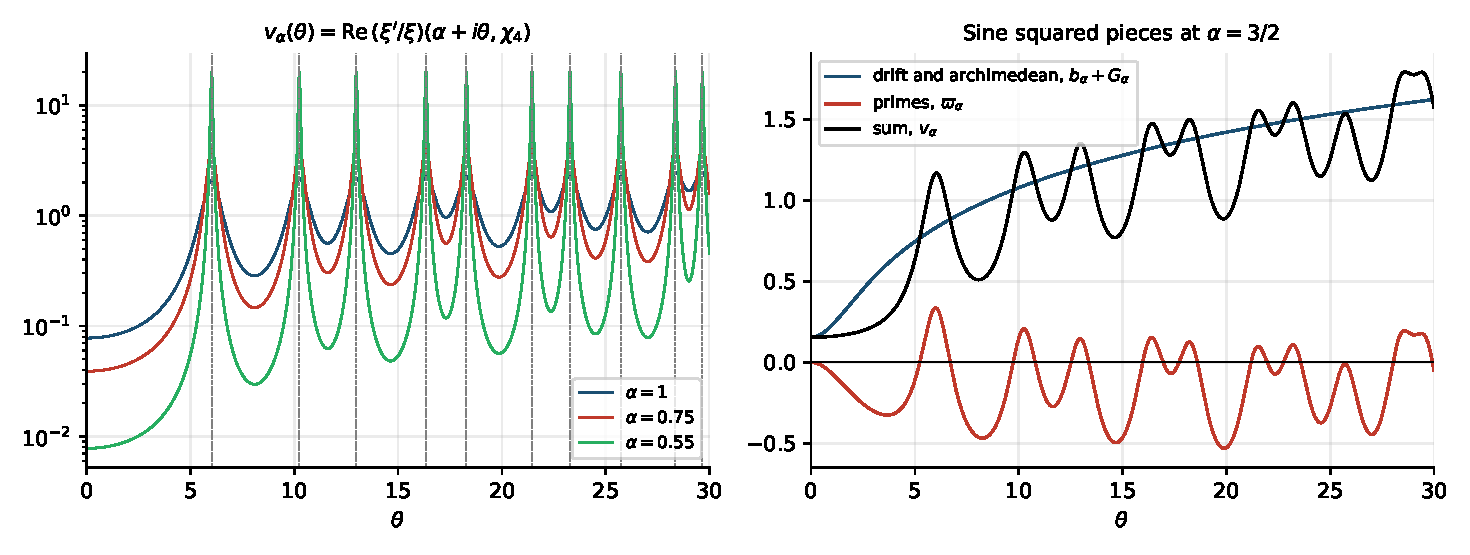
\includegraphics[width=\textwidth]{fig/dbeta_thorin.pdf}
\caption{Left: $v_\alpha(\theta)=\re(\xi'/\xi)(\alpha+i\theta,\chi_4)=\pi\rho_{\alpha-1/2}(\theta)$ for $\alpha=1$, $0.75$, $0.55$ on a logarithmic scale, with the ordinates of the zeros of $L(s,\chi_4)$ (dashed). As $\alpha\downarrow\frac12$ the density concentrates on the ordinates, while its minimum $b_\alpha$, at the origin, tends to zero. Right: at $\alpha=\frac32$, the drift and gamma piece $b_\alpha+G_\alpha$, the prime piece $\varpi_\alpha$, of both signs, and their sum $v_\alpha$. Drawn by \texttt{dbeta\_figs.py}.}
\label{fig:dbeta:thorin}
\end{figure}

\begin{proposition}\label{prop:dbeta:thorin}
For every $\alpha\ge1$, $u\mapsto\xi(\alpha,\chi_4)/\xi(\alpha+\sqrt u,\chi_4)$ is the Laplace transform of a GGC with Thorin density $v_\alpha(\theta)/\pi>0$ in the chart $\theta=\sqrt z$, and \eqref{eq:dbeta:thorinrep} holds. For $\alpha>\frac12$ it is the Laplace transform of a GGC if and only if no zero of $L(s,\chi_4)$ has real part greater than $\alpha$. GRH for $\chi_4$ holds if and only if $v_\alpha\ge0$ for every $\alpha>\frac12$, and the Thorin measures at resolution $\varepsilon=\alpha-\frac12$ converge vaguely, as $\varepsilon\downarrow0$, to the sum of the point masses $\delta_{\gamma^2}$ over the zeros on the critical line, which is the Thorin measure of $\xi(\frac12,\chi_4)/\xi(\frac12+\sqrt u,\chi_4)$ under GRH.
\end{proposition}

\begin{proof}
The proofs of Theorem~\ref{thm:poisson}, of Lagarias's criterion \cite{Lagarias} and of the vague limit stated after Remark~\ref{rem:ch2:oneline} use only the Hadamard product of an entire function of order one whose zeros are symmetric under $\rho\mapsto\bar\rho$ and $\rho\mapsto1-\rho$, with $\sum_\rho|\rho|^{-2}<\infty$; they apply to $\xi(s,\chi_4)$ \cite[Chapter 12]{Davenport}, as Section~\ref{sec:ch16:sin2} and Proposition~\ref{bp:eta:prop:thorin} apply them to $\xi(s,\chi_{12})$. Positivity at $\alpha\ge1$ needs every zero to have real part less than one, which is the absence of zeros of $L(s,\chi_4)$ on $\re s=1$ \cite[Chapter 14]{Davenport} with the Euler product and the functional equation.
\end{proof}

At the basepoint one the clock $T^{(4)}_1$, with Laplace transform $1/\xi(1+\sqrt u,\chi_4)$, therefore has the expansion $1-b_1\sqrt u+O(u)$ at the origin, and as for $\xi$ in \eqref{bp:eq:tail} the Tauberian theorem \cite[XIII.5]{Feller71} gives the tail $P(T^{(4)}_1>x)\sim(b_1/\sqrt\pi)\,x^{-1/2}=0.0438849\,x^{-1/2}$, with $b_1$ from \eqref{eq:dbeta:b1}.

Positivity at $\alpha\ge1$ uses the zeros, not the L\'evy measure. Bounding the prime weights by their absolute values gives positivity only far to the right, and no such bound does better.

\begin{proposition}\label{prop:dbeta:termwise}
For $\alpha>1$ and real $\theta$,
\begin{gather*}
v_\alpha(\theta)\ge A^\infty_4(\alpha,\theta)-S_4(\alpha),\\
A^\infty_4(\alpha,\theta)=\frac12\log\frac4\pi+\frac12\re\psi\Big(\frac{\alpha+1+i\theta}2\Big),\\
S_4(\alpha)=\sum_{n\ \mathrm{odd}}\frac{\Lambda(n)}{n^\alpha}=-\frac{\zeta'}\zeta(\alpha)-\frac{\log2}{2^\alpha-1},
\end{gather*}
and $A^\infty_4(\alpha,\theta)$ increases in $|\theta|$. The bound is positive at every $\theta$ exactly when $\alpha>\alpha_c(\chi_4)=2.2823106368$, the root of $A^\infty_4(\alpha,0)=S_4(\alpha)$. For $\chi_{12}$ the same bound, with $A^\infty_{12}(\alpha,\theta)=\frac12\log\frac{12}\pi+\frac12\re\psi(\frac{\alpha+i\theta}2)$ and $S_{12}(\alpha)=S_4(\alpha)-\log3/(3^\alpha-1)$, is positive at every $\theta$ exactly when $\alpha>\alpha_c(\chi_{12})=1.8348743295$.
\end{proposition}

\begin{proof}
For $\re s>1$,
\[
\frac{\xi'}\xi(s,\chi_4)=\frac12\log\frac4\pi+\frac12\psi\Big(\frac{s+1}2\Big)+\frac{L'}L(s,\chi_4),
\]
and $|\re\frac{L'}L(\alpha+i\theta,\chi_4)|\le\sum_n|\chi_4(n)|\Lambda(n)n^{-\alpha}=S_4(\alpha)$. The series $\re\psi(x+iy)-\psi(x)=\sum_{k\ge0}y^2/\big((x+k)((x+k)^2+y^2)\big)$ shows that $A^\infty_4$ increases in $|\theta|$. Since $A^\infty_4(\alpha,0)$ increases in $\alpha$ and $S_4(\alpha)$ decreases, the root is unique, and \texttt{dbeta\_thorin.py} locates it by bisection with certified signs. For $\chi_{12}$ the primes $2$ and $3$ drop out of the sum.
\end{proof}

In the sine squared form \eqref{eq:dbeta:sin2} the same bound reads $b_\alpha+G_\alpha(\theta)-2\sum_{\chi_4(n)=-1}\Lambda(n)n^{-\alpha}$: the positive atoms are dropped and each negative atom is given its largest value $2$ of $1-\cos$. The smaller value of $\alpha_c$ for $\chi_{12}$ reflects its larger conductor constant $\frac12\log\frac{12}\pi$ and the absence of the primes $2$ and $3$.

\begin{proposition}\label{prop:dbeta:kron}
For $\alpha>1$ and every $T>0$,
\[
\inf_{\theta\ge T}\Big(v_\alpha(\theta)-A^\infty_4(\alpha,\theta)\Big)=\inf_{\theta\ge T}\re\frac{L'}L(\alpha+i\theta,\chi_4)=-S_4(\alpha),
\]
so no lower bound for $\re\frac{L'}L(\alpha+i\theta,\chi_4)$ better than $-S_4(\alpha)$ holds at all large heights. The bound of Proposition~\ref{prop:dbeta:termwise} certifies $v_\alpha(\theta)>0$ exactly for $|\theta|>t_0(\alpha)$, where $A^\infty_4(\alpha,t_0)=S_4(\alpha)$, for $1<\alpha\le\alpha_c$ (so that $t_0(\alpha_c)=0$), and at every real $\theta$ for $\alpha>\alpha_c$, and
\[
\log t_0(\alpha)=\frac2{\alpha-1}-2\gamma_E-\log\frac8\pi+O(\alpha-1),\qquad\alpha\downarrow1,
\]
with $-2\gamma_E-\log\frac8\pi=-2.0891$.
\end{proposition}

\begin{proof}
From the Euler product, $\re\frac{L'}L(\alpha+i\theta,\chi_4)=-\sum_p\log p\,\re\frac{w_p}{1-w_p}$ with $w_p=\chi_4(p)p^{-\alpha-i\theta}$, and on the circle $|w|=r<1$ the maximum of $\re\frac w{1-w}=\re\frac1{1-w}-1$ is $\frac r{1-r}$, at $w=r$; this gives the lower bound $-S_4(\alpha)$. Since the numbers $\log p$ are linearly independent over $\mathbb Q$, Kronecker's theorem \cite[Chapter 23]{boHardyWright} gives, for every $P$ and $\eta>0$, a height $\theta\ge T$ at which $|\chi_4(p)p^{-i\theta}-1|<\eta$ for all odd $p\le P$, and the primes beyond $P$ contribute at most $\sum_{p>P}\log p\,p^{-\alpha}/(1-p^{-\alpha})$, which is small for $P$ large. For the asymptotic, $S_4(\alpha)=\frac1{\alpha-1}-\gamma_E-\log2+O(\alpha-1)$ and $A^\infty_4(\alpha,t)=\frac12\log\frac{2t}\pi+O(t^{-2})$ as $t\to\infty$, uniformly for $1\le\alpha\le2$, from $\psi(z)=\log z-\frac1{2z}+O(|z|^{-2})$; solving $A^\infty_4(\alpha,t_0)=S_4(\alpha)$ gives the formula, since $t_0(\alpha)\to\infty$.
\end{proof}

\begin{table}[htbp]
\centering\small
\begin{tabular}{cccc}
\toprule
$\alpha$ & $S_4(\alpha)$ & $t_0(\alpha)$ & $\log t_0(\alpha)-\frac2{\alpha-1}$\\
\midrule
$2$ & $0.33891193$ & $2.36723$ & $-1.1383$\\
$1.75$ & $0.57950941$ & $4.71677$ & $-1.1155$\\
$1.5$ & $1.1261406$ & $14.8728$ & $-1.3005$\\
$1.25$ & $2.9637961$ & $589.44$ & $-1.6208$\\
$1.1$ & $8.8348984$ & $7.41336\times10^7$ & $-1.8786$\\
$1.05$ & $18.784554$ & $3.25219\times10^{16}$ & $-1.9793$\\
\bottomrule
\end{tabular}
\caption{The height $t_0(\alpha)$ above which the bound of Proposition~\ref{prop:dbeta:termwise} certifies $v_\alpha>0$, for basepoints below $\alpha_c(\chi_4)=2.2823$; the last column tends to $-2\gamma_E-\log\frac8\pi=-2.0891$ (Proposition~\ref{prop:dbeta:kron}). Computed by \texttt{dbeta\_thorin.py}.}
\label{tab:dbeta:kron}
\end{table}

So for $1<\alpha<\alpha_c$ the absolute values of the weights reduce the positivity of $v_\alpha$ to a computation on $[0,t_0(\alpha)]$, but $t_0$ grows like $e^{2/(\alpha-1)}$ (Table~\ref{tab:dbeta:kron}). At $\alpha=1$ the prime piece converges only conditionally, by the prime number theorem for progressions, whose analytic input is the absence of zeros of $L(s,\chi_4)$ on $\re s=1$; the positivity of $v_1$, which Proposition~\ref{prop:dbeta:thorin} draws from that input, cannot come from the sizes of the weights. (Dirichlet's theorem for the modulus $4$ itself needs only $L(1,\chi_4)=\frac\pi4\ne0$.)

\subsubsection{The Gaussian field}\label{sec:dbeta:qi}

The pairing of the primes $p\equiv1$ and $p\equiv3\pmod4$ is their splitting in $K=\mathbb Q(i)$: a prime $p\equiv1\pmod4$ splits into two Gaussian primes of norm $p$, and a prime $p\equiv3\pmod4$ stays prime, with norm $p^2$. Accordingly $\zeta_K(s)=\zeta(s)L(s,\chi_4)$, and in the normalisation of Section~\ref{sec:sqfree:nf},
\[
\xi_K(s)=2s(s-1)\pi^{-s}\Gamma(s)\zeta_K(s)=\xi(s)\,\xi(s,\chi_4),
\]
by the duplication formula $\Gamma(s)=2^{s-1}\pi^{-1/2}\Gamma(\frac s2)\Gamma(\frac{s+1}2)$. Write $v^K_\alpha$ and $v^\xi_\alpha$ for the brackets $\re(\xi_K'/\xi_K)(\alpha+i\theta)$ and $\re(\xi'/\xi)(\alpha+i\theta)$, and $v_\alpha$ as before for $\chi_4$.

\begin{proposition}\label{prop:dbeta:factor}
On every vertical line, $v_\alpha=v^K_\alpha-v^\xi_\alpha$. For $\alpha>1$ the canonical measure of $\xi_K$ at the basepoint $\alpha$ is
\[
x\Pi^K_\alpha(dx)=\Big(\frac{e^{-(\alpha+1)x}}{1-e^{-x}}-e^{-(\alpha-1)x}\Big)dx+\sum_{n\ge2}\frac{(1+\chi_4(n))\Lambda(n)}{n^\alpha}\,\delta_{\log n}(dx),
\]
and the canonical measure of Proposition~\ref{prop:dbeta:levy} is $x\Pi_\alpha=x\Pi^K_\alpha-x\Pi^\xi_\alpha$, with $x\Pi^\xi_\alpha$ that of Section~\ref{bp:sec:levy}: the pole densities $-e^{-(\alpha-1)x}$ cancel, the gamma densities differ by $e^{-\alpha x}/(2\sinh x)$, and the atoms by $\chi_4(n)\Lambda(n)n^{-\alpha}$.
\end{proposition}

\begin{proof}
Take logarithmic derivatives in $\xi_K=\xi\cdot\xi(\cdot,\chi_4)$. For the measures write $\xi_K(s)=(s-1)\cdot2\pi^{-s}\Gamma(s+1)\zeta_K(s)$: Binet's formula for $\Gamma(s+1)$ at $\alpha$ gives the density $e^{-(\alpha+1)x}/(x(1-e^{-x}))$, the factor $s-1$ gives $-e^{-(\alpha-1)x}/x$ as for $\xi$, and $-\frac{\zeta_K'}{\zeta_K}=-\frac{\zeta'}\zeta-\frac{L'}L$ has the coefficients $(1+\chi_4(n))\Lambda(n)\ge0$. Finally $\frac{e^{-(\alpha+1)x}}{1-e^{-x}}-\frac{e^{-(\alpha+2)x}}{1-e^{-2x}}=e^{-\alpha x}\Big(\frac1{e^x-1}-\frac1{e^{2x}-1}\Big)=\frac{e^{-\alpha x}e^x}{e^{2x}-1}=\frac{e^{-\alpha x}}{2\sinh x}$.
\end{proof}

\begin{corollary}\label{cor:dbeta:dom}
\textup{(i)} For every $\alpha\ge1$ there are independent GGC variables $H^\xi_\alpha$ and $H^{(4)}_\alpha$, with Laplace transforms $\xi(\alpha)/\xi(\alpha+\sqrt u)$ and $\xi(\alpha,\chi_4)/\xi(\alpha+\sqrt u,\chi_4)$, whose sum $H^K_\alpha=H^\xi_\alpha+H^{(4)}_\alpha$ is the GGC with Laplace transform $\xi_K(\alpha)/\xi_K(\alpha+\sqrt u)$ and Thorin density $v^K_\alpha/\pi$.

\textup{(ii)} GRH for $\chi_4$ holds if and only if $v^K_\alpha\ge v^\xi_\alpha$ on every line $\re s=\alpha>\frac12$: the Thorin density of $\xi_K$ dominates that of $\xi$ at every basepoint.

\textup{(iii)} Under RH, GRH for $\chi_4$ holds if and only if, for every $\alpha>\frac12$, $\xi_K(\alpha)/\xi_K(\alpha+\sqrt u)$ is the Laplace transform of $H^\xi_\alpha+H$ for some GGC $H$ independent of $H^\xi_\alpha$.
\end{corollary}

\begin{proof}
(i) By Theorem~\ref{thm:poisson} and Proposition~\ref{prop:dbeta:thorin} both factors are GGC transforms for $\alpha\ge1$, and transforms of independent sums multiply. (ii) By Proposition~\ref{prop:dbeta:factor}, $v^K_\alpha\ge v^\xi_\alpha$ is $v_\alpha\ge0$, and Proposition~\ref{prop:dbeta:thorin} applies. (iii) Under RH, $H^\xi_\alpha$ is a GGC for every $\alpha>\frac12$ (Theorem~\ref{thm:poisson}). If GRH holds for $\chi_4$, take $H=H^{(4)}_\alpha$. Conversely, the transform of $H$ is then $\xi(\alpha,\chi_4)/\xi(\alpha+\sqrt u,\chi_4)$, and if it is a GGC transform for every $\alpha>\frac12$, Proposition~\ref{prop:dbeta:thorin} gives GRH.
\end{proof}

Neither $v^K_\alpha$ nor $v^\xi_\alpha$ is positive term by term: each has the pole piece $-\theta^2/\big((\alpha-1)((\alpha-1)^2+\theta^2)\big)$ of \eqref{eq:split}, and the two cancel in the difference, which is why $\xi(s,\chi_4)$ has none. The factorisation is the right language for the pairing of the primes, but it does not by itself lower $\alpha_c$: by Proposition~\ref{prop:dbeta:kron} any argument that uses only the sizes of the weights reaches no further. Table~\ref{tab:dbeta:qi} shows the three brackets at $\alpha=\frac32$; \texttt{dbeta\_thorin.py} checks $v^K_\alpha-v^\xi_\alpha-v_\alpha=0$ there to $10^{-36}$, and the identity $\xi_K=\xi\cdot\xi(\cdot,\chi_4)$ at $s=0.3+4.1i$, where both sides are $0.21807580405390-0.037869233276222i$ after division by $\xi(s)$, and at $s=2.5$.

\begin{table}[htbp]
\centering\small
\begin{tabular}{cccccc}
\toprule
$\theta$ & $0$ & $2$ & $5$ & $10$ & $20$\\
\midrule
$v^K_{3/2}(\theta)$ & $0.200351$ & $0.225243$ & $0.685189$ & $1.32766$ & $1.49863$\\
$v^\xi_{3/2}(\theta)$ & $0.0461359$ & $0.0470396$ & $0.0526739$ & $0.102889$ & $0.606114$\\
$v_{3/2}(\theta)$ & $0.154215$ & $0.178204$ & $0.632515$ & $1.22477$ & $0.892517$\\
\bottomrule
\end{tabular}
\caption{The brackets of $\xi_{\mathbb Q(i)}$, $\xi$ and $\xi(\cdot,\chi_4)$ at the basepoint $\frac32$; the last row is the difference of the first two (Proposition~\ref{prop:dbeta:factor}). Computed by \texttt{dbeta\_thorin.py}.}
\label{tab:dbeta:qi}
\end{table}

The same holds for every real primitive character $\chi_D$, with $D$ a fundamental discriminant and $K=\mathbb Q(\sqrt D)$: $\xi_K$ is a constant multiple of $\xi\cdot\xi(\cdot,\chi_D)$, the constant being $2/\sqrt{|D|}$ for $D<0$ (Section~\ref{sec:sqfree:quad}) and $2$ for $D>0$, since then $\xi_K(s)=s(s-1)D^{s/2}\Gamma_{\mathbb R}(s)^2\zeta_K(s)$ and $\xi(s,\chi_D)=D^{s/2}\Gamma_{\mathbb R}(s)L(s,\chi_D)$. So $v^{(\chi_D)}_\alpha=v^K_\alpha-v^\xi_\alpha$; the GGC property at every $\alpha\ge1$, the equivalence of GRH for $\chi_D$ with the domination of the Thorin density of $\xi$ by that of $\xi_K$, and the localisation of Corollary~\ref{cor:dbeta:argmono} hold for $\xi(s,\chi_D)$ with the same proofs. For $\chi_{12}$, $K=\mathbb Q(\sqrt3)$, and the numbers are: $\alpha_c(\chi_{12})=1.8348743295$ (Proposition~\ref{prop:dbeta:termwise}); $V_{12}=(\log\xi)''(\frac12,\chi_{12})=0.332923608212$; and at $\alpha=1$, $0.75$ and $0.6$ the drift $b_\alpha$ is $0.1650833$, $0.0830566$ and $0.0332812$, the minimum of $v_\alpha$ on a grid of step $0.01$ on $[0,60]$, attained at the origin (\texttt{dbeta\_minimum.py}), as Theorem~\ref{thm:dbeta:minall} proves at every height for $\alpha\ge1$ and on the verified range for $\frac12<\alpha<1$. The script \texttt{dbeta\_zeros.py} certifies the first five ordinates of $L(s,\chi_{12})$, $3.8046276331$, $6.6922233205$, $8.8905929587$, $11.1883927451$ and $12.9661788080$, all simple and on the critical line, in agreement with Section~\ref{sec:ch16:eta}; their largest gap, the first, $2.8876$, lies below $2/\sqrt{V_{12}}=3.4662$, and below the value $3.3189$ at $a=\frac12$ of the threshold of Remark~\ref{rem:dbeta:nearest} for $\chi_{12}$. On the real axis the same script gives $L(\sigma,\chi_{12})=0.1246437042$, $0.3344871142$, $0.4985570025$, $0.6250274399$ and $0.7213905658$ at $\sigma=0.1$, $0.3$, $0.5$, $0.7$ and $0.9$, positive, as the positivity of the kernel requires.

\begin{question}\label{q:dbeta:coupling}
Is there a construction of $H^K_\alpha=H^\xi_\alpha+H^{(4)}_\alpha$ from the Gaussian primes themselves, two of norm $p$ for each $p\equiv1$ and one of norm $p^2$ for each $p\equiv3\pmod4$, that persists below the basepoint one? By Proposition~\ref{prop:dbeta:kron} such a construction must see the phases $p^{-i\theta}$, not only the sizes of the weights; below $\alpha=1$ its existence is equivalent to GRH for $\chi_4$ under RH, by Corollary~\ref{cor:dbeta:dom}(iii). In the language of Section~\ref{sec:dbeta:arg}, the decomposition is the additivity $\arg\xi_K=\arg\xi+\arg\xi(\cdot,\chi_4)$ on vertical lines, and the domination of Corollary~\ref{cor:dbeta:dom}(ii) says that $\arg\xi_K-\arg\xi$ is nondecreasing on every line $\re s=\alpha>\frac12$.
\end{question}

\subsubsection{The Thorin measure as an argument}\label{sec:dbeta:arg}

The density $v_\alpha(\theta)$ is the derivative in $\theta$ of the argument of $\xi(\alpha+i\theta,\chi_4)$, so the Thorin measure on a vertical line is an argument, and at the centre a zero count.

\begin{proposition}\label{prop:dbeta:arg}
Let $\alpha>\frac12$ be such that no zero of $\xi(s,\chi_4)$ lies on the line $\re s=\alpha$; this holds for every $\alpha\ge1$. Then for $\theta>0$
\[
\frac1\pi\int_0^\theta v_\alpha(t)\,dt=\frac1\pi\arg\xi(\alpha+i\theta,\chi_4),
\]
with the argument continuous along the segment from $\alpha$ to $\alpha+i\theta$ and zero at $\alpha$; for $\alpha\ge1$ the left side is the mass of $(0,\theta^2]$ under the Thorin measure of Proposition~\ref{prop:dbeta:thorin}. As $\theta\to\infty$, with $a=\frac{\alpha+1}2$,
\[
\frac1\pi\arg\xi(\alpha+i\theta,\chi_4)=\frac\theta{2\pi}\log\frac{2\theta}{\pi e}+\frac\alpha4+\frac1\pi\arg L(\alpha+i\theta,\chi_4)-\frac{a(a-1)+\frac16}{\pi\theta}+O(\theta^{-3}),
\]
with $\arg L$ continuous along the same segment. As $\alpha\downarrow\frac12$, for $\theta$ not an ordinate, the left side tends to the number of zeros on the critical line with $0<\gamma<\theta$, which is $N(\theta)$ under GRH; at $\alpha=\frac12$ the expansion is the counting formula \eqref{eq:dbeta:count}.
\end{proposition}

\begin{proof}
Since $\frac{d}{dt}\log\xi(\alpha+it,\chi_4)=i\frac{\xi'}\xi(\alpha+it,\chi_4)$, the derivative of $\arg\xi(\alpha+it,\chi_4)=\im\log\xi(\alpha+it,\chi_4)$ is $v_\alpha(t)$, and $\xi(\alpha,\chi_4)>0$. The expansion is $\frac\theta2\log\frac4\pi$ plus Stirling's series $\log\Gamma(z)=(z-\frac12)\log z-z+\frac12\log2\pi+\frac1{12z}+O(|z|^{-3})$ \cite[\S5.11]{DLMF} at $z=a+\frac{i\theta}2$: with $y=\frac\theta2$,
\[
\im\log\Gamma(a+iy)=y\log y-y+\frac\pi2\Big(a-\frac12\Big)-\Big(\frac{a(a-1)}2+\frac1{12}\Big)\frac1y+O(y^{-3}),
\]
from $\arg z=\frac\pi2-\frac ay+O(y^{-3})$ and $\log|z|=\log y+\frac{a^2}{2y^2}+O(y^{-4})$; and $\frac\theta2\log\frac4\pi+\frac\theta2\log\frac\theta2-\frac\theta2=\frac\theta2\log\frac{2\theta}{\pi e}$, $\frac12(a-\frac12)=\frac\alpha4$. For the limit, write $v_\alpha$ by the Hadamard product, as in Proposition~\ref{prop:struct}, as the absolutely convergent sum over the zeros $\rho=\beta+i\gamma$ of $(\alpha-\beta)/((\alpha-\beta)^2+(t-\gamma)^2)$; each term integrates over $[0,\theta]$ to $\arctan\frac{\theta-\gamma}{\alpha-\beta}+\arctan\frac\gamma{\alpha-\beta}$, which for a zero on the line tends to $\pi$ if $0<\gamma<\theta$ and to $0$ if $\gamma>\theta$ or $\gamma<0$, while the two terms of an off line pair $\frac12\pm\delta+i\gamma$ have the limits $\mp\big(\arctan\frac{\theta-\gamma}\delta+\arctan\frac\gamma\delta\big)$, which cancel. The terms are dominated by $\pi$ and by $C\theta/\gamma^2$ for $|\gamma|>2\theta+1$, uniformly for $\frac12<\alpha\le1$, so dominated convergence applies. At $\alpha=\frac12$, $a=\frac34$ and $a(a-1)+\frac16=-\frac1{48}$.
\end{proof}

The Thorin measure at resolution $\varepsilon=\alpha-\frac12$ is therefore the zero counting function smoothed by the Cauchy kernel of width $\varepsilon$; this is the analogue for $\chi_4$ of the cumulative Thorin mass of $\xi$ as a smoothed counting function (Section~\ref{sec:ch9:mass}). The script \texttt{dbeta\_thorin.py} continues $\arg\xi(\alpha+i\theta,\chi_4)$ in ball arithmetic, as \texttt{dbeta\_zeros.py} does, and integrates $v_\alpha$ by quadrature: at $(\alpha,\theta)=(1.5,10)$, $(1.5,25)$ and $(2,30)$ both sides are $1.65731473994$, $7.40149777268$ and $9.85153586211$. At $\alpha=0.75$ the difference between the left side and the first three terms of the expansion is $-3.65\times10^{-4}$, $-1.82\times10^{-4}$ and $-9.12\times10^{-5}$ at $\theta=50$, $100$ and $200$, that is $-0.0182/\theta$, against $-(a(a-1)+\frac16)/\pi=-11/(192\pi)=-0.018237$ at $a=\frac78$.

\begin{corollary}\label{cor:dbeta:argmono}
GRH for $\chi_4$ holds if and only if, for every $\alpha>\frac12$, $\theta\mapsto\arg\xi(\alpha+i\theta,\chi_4)$ is nondecreasing. With no hypothesis, the heights $\theta>0$ at which it decreases lie in the union of the windows $|\theta-\gamma|<\sqrt{\delta^2-(\alpha-\frac12)^2}$, each of length less than $1$, over the zeros $\frac12+\delta+i\gamma$ with $\delta>\alpha-\frac12$, and there are none at heights below $2.5\times10^7-\frac12$.
\end{corollary}

\begin{proof}
The derivative is $v_\alpha(\theta)$, and Proposition~\ref{prop:dbeta:thorin} gives the equivalence. By the Hadamard product, $v_\alpha$ is a sum of positive Cauchy kernels, one for each zero on the line and two for each off line pair $\frac12\pm\delta+i\gamma$ with $\delta\le\alpha-\frac12$, plus, for each pair with $\delta>\alpha-\frac12$, the difference $\pi\big(P_{\varepsilon+\delta}-P_{\delta-\varepsilon}\big)(\theta\mp\gamma)$ with $\varepsilon=\alpha-\frac12$, which is negative exactly where $|\theta\mp\gamma|<\sqrt{\delta^2-\varepsilon^2}$ (proof of Proposition~\ref{prop:signature}(ii)); for $\theta>0$ and $\gamma>0$ the reflected term at $\theta+\gamma$ is positive, since $\theta+\gamma>\gamma>\delta$. A window has length $2\sqrt{\delta^2-\varepsilon^2}<2\delta<1$. Platt's verification of GRH for the modulus $4$ to height $10^8/4$ \cite{Platt16} puts every zero off the line above $2.5\times10^7$, and so every window above $2.5\times10^7-\frac12$.
\end{proof}

A window holds a decrease only if the negative term of its pair outweighs all the positive terms there, and the decrease is bounded: the negative part of the term $\pi(P_{\varepsilon+\delta}-P_{\delta-\varepsilon})(\theta-\gamma)$ of a pair has integral $4\arctan\sqrt{(\delta+\varepsilon)/(\delta-\varepsilon)}-\pi<\pi$, by Proposition~\ref{prop:signature}(iii), so over any interval the argument falls by less than $\pi$ times the number of pairs whose windows meet it, whatever the other zeros, and the fall caused by a pair tends to zero as $(\alpha-\frac12)/\delta\to0$. This answers the quantitative half of a question of the first author's note. No lower bound for the positive terms over a window, such as a mean value estimate for the contribution of the zeros on the line, can exclude this for every pair: at the centre $\theta=\gamma$ of its window the pair contributes $\frac1{\varepsilon+\delta}-\frac1{\delta-\varepsilon}=-\frac{2\varepsilon}{\delta^2-\varepsilon^2}$, which is unbounded below as $\delta\downarrow\varepsilon$, that is as the zero approaches the line $\re s=\alpha$ from the right, while by Lemma~\ref{ag:lem:cancel} a zero far enough to the right of the line cannot produce a decrease against a given positive floor. Outside the strips $|\theta-\gamma|<(1+\sqrt2)\delta$ around the ordinates of the zeros off the line, Theorem~\ref{thm:dbeta:comp} gives the argument a rate of increase that grows like $\log\theta$ (Corollary~\ref{cor:dbeta:lower}). Figure~\ref{fig:dbeta:arg} shows the smoothing, and the minimum at the origin that Section~\ref{sec:dbeta:comp} proves.

\begin{figure}[htbp]
\centering
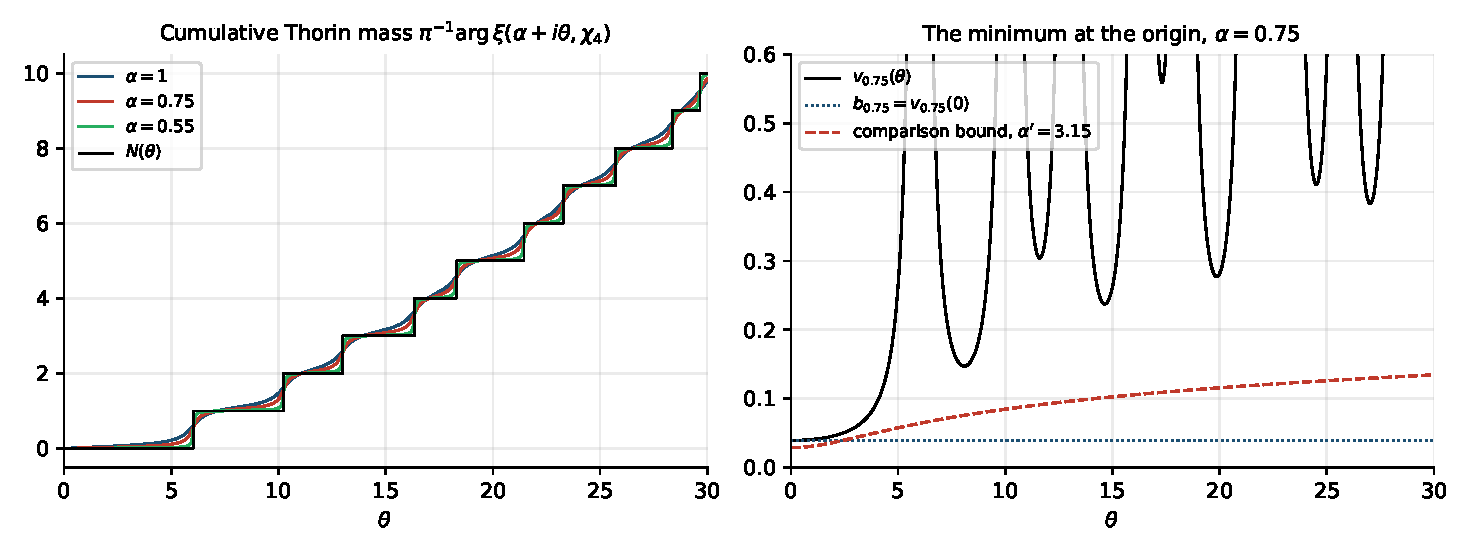
\includegraphics[width=\textwidth]{fig/dbeta_argument.pdf}
\caption{Left: the cumulative Thorin mass $\frac1\pi\arg\xi(\alpha+i\theta,\chi_4)=\frac1\pi\int_0^\theta v_\alpha$ for $\alpha=1$, $0.75$ and $0.55$, against the zero count $N(\theta)$ of $L(s,\chi_4)$; at $\theta=30$ the masses are $9.7747$, $9.8405$ and $9.9621$, and $N(30)=10$. The argument is continued through the quotients of values at steps of $0.005$, each of argument below $0.11$ in modulus. Right: $v_{0.75}(\theta)$, its minimum $b_{0.75}=0.0389784$ at the origin, and the lower bound of Corollary~\ref{cor:dbeta:lower} with $\alpha'=3.15$, which exceeds $b_{0.75}$ for $\theta>2.434$ (\texttt{dbeta\_minimum.py}). Drawn by \texttt{dbeta\_figs.py}.}
\label{fig:dbeta:arg}
\end{figure}

\subsubsection{The centre}\label{sec:dbeta:centre}

For $\zeta$ the positive structure at the centre is the Thorin measure of the clock, not a structure of the P\'olya variable itself (Proposition~\ref{sb:prop:qid}(1)). The same holds for $\chi_4$. The characteristic function $\xi(\frac12+i\theta,\chi_4)/\xi(\frac12,\chi_4)$ of $Y_4$ is real and changes sign at $\gamma_1=6.0209489$, where it passes from $0.00607732$ at $\theta=5.9$ to $-0.00350813$ at $\theta=6.1$, and at each of the other ordinates below height $100$; Hardy's argument for $\zeta$ \cite[Chapter 10]{Titchmarsh}, applied to the theta series $\eta(ix)^3$ of $\chi_4$, gives infinitely many such sign changes. So $Y_4$ is not quasi infinitely divisible, and in particular not infinitely divisible: a quasi infinitely divisible characteristic function never vanishes. Nor is $\xi(\frac12+w,\chi_4)/\xi(\frac12,\chi_4)$ a positive mixture $\int M(d\lambda)/(w+\lambda)^2$ of Gamma(2) transforms, for a more elementary reason: such a mixture decreases on $w>0$, while $\xi(\frac12+w,\chi_4)=\int_{\R}K_4(u)\cosh(wu)\,du$ increases there. A one sided object remains, the half kernel $K_4(u)\mathbf 1\{u>0\}$, and it is not a positive gamma mixture either.

\begin{proposition}\label{prop:dbeta:nocm}
For no $a>0$ is $u^{1-a}K_4(u)$ completely monotone on $u>0$; in particular the half kernel is not a positive mixture of Gamma($a$) densities $u^{a-1}e^{-\lambda u}$, for any shape $a$. The theta function $\eta(ix)^3$ is not completely monotone on $x>0$.
\end{proposition}

\begin{proof}
If $g(u)=\int_{[0,\infty)}e^{-\lambda u}M(d\lambda)$ with $M\ge0$ and $M\ne0$, choose $L$ with $M([0,L])>0$; then $g(u)\ge M([0,L])e^{-Lu}$, so $g$ decays at most exponentially, while $u^{1-a}K_4(u)$ decays like $\exp(-\frac\pi4e^{2u})$ (Proposition~\ref{prop:dbeta:kernel}). The Jacobi series $\eta(ix)^3=\sum_{n\ge0}(-1)^n(2n+1)e^{-\pi(2n+1)^2x/4}$ is the Laplace transform of the signed measure with the weights $(-1)^n(2n+1)$ at the points $\pi(2n+1)^2/4$, which by the uniqueness of the Laplace transform is its only representing measure, and it is not positive, so Bernstein's theorem excludes complete monotonicity.
\end{proof}

The decay argument applies to the kernel of every completed $L$ function of degree one, all of which decay like $\exp(-ce^{2|u|})$; for $\xi$ it shows that no positive mixture of Gamma($a$) densities represents the P\'olya kernel on the half line, for any shape $a$, as \cite[Section 13.6]{P17} observes (see also \cite[Section 12.6]{P26}).

The positive structure is in the reciprocal of the product. With $q=e^{-2\pi x}$,
\begin{equation}\label{eq:dbeta:recip}
\frac{e^{-\pi x/4}}{\eta(ix)^3}=\prod_{m\ge1}\big(1-q^m\big)^{-3}=\exp\Big(3\sum_{N\ge1}\sigma_{-1}(N)\,e^{-2\pi Nx}\Big),\qquad\sigma_{-1}(N)=\sum_{d\mid N}\frac1d,
\end{equation}
from $-\log(1-q^m)=\sum_kq^{mk}/k$; so the logarithm of the left side is completely monotone, and hence so is the left side, the exponential of a completely monotone function being completely monotone. At $x=0.3$ the three forms agree to fifteen digits, $1.77964734678018$ (\texttt{dbeta\_thorin.py}). In the language of Section~\ref{sec:ch16:max}, $\prod_m(1-e^{-2\pi mx})^3$ is the distribution function of the maximum $M_3$ of independent exponential variables, three of each rate $2\pi m$, and \eqref{eq:dbeta:recip} is the complete monotonicity of minus the logarithm of such a distribution function noted in Section~\ref{sec:ch16:dbn}, with the masses $3\sigma(N)/N$. The representation of Section~\ref{sec:ch16:max} also carries over: since $\eta(ix)^3=e^{-\pi x/4}\Pr(M_3\le x)$ and $x^{c-1}e^{-\pi x/4}(\pi/4)^c/\Gamma(c)$ is the density of $\frac4\pi G_c$, with $G_c$ a gamma variable of shape $c$ independent of $M_3$, the Mellin form gives $\xi(s,\chi_4)=(\frac4\pi)^c\Gamma(c)\Pr(\frac4\pi G_c\ge M_3)$ with $c=\frac{s+1}2$, that is
\[
L(s,\chi_4)=\Pr\big(4G_{(s+1)/2}\ge\pi M_3\big),\qquad s>-1,
\]
which at $s=1$ is $\E e^{-\pi M_3/4}=\frac\pi4\int_0^\infty\eta(ix)^3dx=\frac\pi4$.

The half kernel has the Laplace transform
\begin{equation}\label{eq:dbeta:incomplete}
\int_0^\infty e^{-wu}K_4(u)\,du=A_4\big(\tfrac12-w\big),
\end{equation}
where
\[
A_4(s)=\int_1^\infty\eta(ix)^3x^{(s+1)/2}\frac{dx}x=\sum_{n\ge1}\chi_4(n)\,n\,\frac{\Gamma(\frac{s+1}2,\frac{\pi n^2}4)}{(\pi n^2/4)^{(s+1)/2}}
\]
is an incomplete Mellin transform of $\eta^3$, and the transformation $\eta(i/x)^3=x^{3/2}\eta(ix)^3$, applied to the integral over $(0,1)$, gives $\xi(s,\chi_4)=A_4(s)+A_4(1-s)$ for every $s$. This is the analogue of Riemann's formula (Proposition~\ref{prop:maxexp:riemann}) and of the symmetric form \eqref{eq:maxexp:sym} for $\Delta$, with no pole terms, since $\eta(ix)^3$ has no constant term. At $w=0.3$ both sides of \eqref{eq:dbeta:incomplete} are $0.44608019686738$, and $A_4(0.2)+A_4(0.8)=\xi(0.2,\chi_4)=0.98762005303445$ (\texttt{dbeta\_thorin.py}).

\begin{question}\label{q:dbeta:recip}
Can the complete monotonicity of \eqref{eq:dbeta:recip}, and of its analogue $\prod_m(1-q^m)^{-1}$ for the kernel of $\chi_{12}$, be turned into a positive representation on the reciprocal side, in the spirit of Thorin's construction for the reciprocal of a GGC transform?
\end{question}

\section{The inverse problem: recovering the atoms by nonnegative deconvolution}\label{ch:deconv}

We return to $\zeta$. The distances of Section~\ref{ch:distances} compare its Thorin density with the Poisson smoothing of a known list of zeros; the inverse problem is to recover the zeros from the density alone. Under RH the density is the Poisson smoothing of a positive measure with an atom at each zero, so the recovery is a deconvolution under a positivity constraint, and RH on a window becomes a feasibility question. The monograph \cite[Section 19.3]{P26} poses it as a Bayesian problem with a positivity prior and a posterior predictive check, and notes that the experiment had not been run because $\rho_\varepsilon$ was available only from the primes, at resolutions above one half. The P\'olya route of Section~\ref{ch:polya} supplies $\rho_\varepsilon$ at small resolution to about $60$ digits below height $200$ (Section~\ref{sec:ch4:trapezoid}); the experiment uses it in double precision. At $\varepsilon=0.1$ a nonnegative least squares fit recovers the ten zeros in $[15,55]$ to within $10^{-5}$, with unit masses, and a displaced zero raises the residual roughly like the square of its displacement.

\subsection{Recovering the zeros by nonnegative least squares}\label{sec:ch17:nnls}

Write $P_\varepsilon(x)=\varepsilon/(\pi(\varepsilon^2+x^2))$ and $U^\pm_{\RH}=\sum_{\gamma>0}(\delta_\gamma+\delta_{-\gamma})$. Under RH, $\rho_\varepsilon=P_\varepsilon*U^\pm_{\RH}$ on $\theta>0$ (Proposition~\ref{prop:struct}); since $P_\varepsilon$ has Fourier transform $e^{-\varepsilon|t|}$, recovering $U^\pm_{\RH}$ is severely ill posed. An off line pair $\frac12\pm\delta+i\gamma$ with $\delta<\varepsilon$ contributes $P_{\varepsilon+\delta}+P_{\varepsilon-\delta}$ at $\gamma$, where two line zeros would contribute $2P_\varepsilon$, and $P_{\varepsilon-\delta}$ is sharper than the Poisson smoothing at level $\varepsilon$ of any positive measure, since $P_{\varepsilon-\delta}=P_\varepsilon*\lambda$ would give $\lambda$ the exponentially growing Fourier transform $e^{\delta|t|}$. Positivity of the recovered measure is therefore the test.

Fix a data window $[\theta_a,\theta_b]$ with sample points $\theta_1<\dots<\theta_n$, and candidate atom locations $x_1<\dots<x_m$ on a grid over a candidate window $[x_a,x_b]$ that contains $[\theta_a,\theta_b]$. With $A_{ij}=P_\varepsilon(\theta_i-x_j)+P_\varepsilon(\theta_i+x_j)$ and data $y_i=\rho_\varepsilon(\theta_i)-b_i$, where $b_i$ is the contribution of the zeros outside the candidate window, the problem is
\[
\min_{w\ge0}\ \|Aw-y\|_2 .
\]
Under a Gaussian likelihood with a flat prior on the positive orthant its solution is the maximum a posteriori estimate, and the minimal residual is the discrepancy statistic of the posterior predictive check: up to the error of the grid, it vanishes when the data are the Poisson smoothing of a positive measure. With data exact to double precision there is no noise level, and the check is a feasibility test. The active set algorithm of Lawson and Hanson \cite{LawsonHanson74} solves the problem in finitely many steps; we use its implementation in \texttt{scipy}. The generative approach of \cite[Section 19.2]{P26} would replace the optimisation by a learned map from data to posterior samples, but the optimisation is deterministic, and its output can be compared atom by atom with the known zeros.

We took $\varepsilon=0.1$, the P\'olya computed $\rho_{0.1}$ on $[15,55]$ at $1601$ points (spacing $0.025$), and candidates on $[5,65)$ at spacing $0.02$ ($3000$ columns). The background $b_i$ is the Poisson smoothing of the zeros outside $[5,65]$ among the first $1700$ ordinates, the list of Section~\ref{ch:distances} without its smooth tail, which would add about $3\times10^{-5}$ to each sample; no ordinate inside the candidate window enters the fit. The nonnegative solution concentrates on clusters, runs of adjacent grid points with weights above $10^{-3}$, one at each zero in the data window (Table~\ref{tab:ch17:atoms} and Figure~\ref{fig:ch17:deconv}, left): every ordinate is recovered to within $10^{-5}$, with mass one to within half a per cent. The remaining mass, $0.071$ of the total $10.094$, lies in small clusters at the edges of the data window ($0.025$), which absorb the tails of the zeros at $14.13$ and $56.45$ just outside it, and in weights below $10^{-3}$ ($0.046$). The residual norm is $0.106$, a root mean square of $0.0026$ against peaks of height $1/(\pi\varepsilon)=3.18$. It is set by the grid: the true atoms lie between grid points, and a positive combination of two neighbouring Cauchy kernels reproduces an off grid kernel only to second order in the grid spacing.

\begin{table}[htbp]
\centering\small
\begin{tabular}{rrrrr}
\toprule
$k$ & $\gamma_k$ & $c_k$ & $10^6(c_k-\gamma_k)$ & mass\\
\midrule
2 & 21.022040 & 21.022034 & $-5.5$ & 1.0013\\
3 & 25.010858 & 25.010859 & $1.6$ & 1.0027\\
4 & 30.424876 & 30.424867 & $-8.8$ & 1.0020\\
5 & 32.935062 & 32.935070 & $8.7$ & 1.0020\\
6 & 37.586178 & 37.586171 & $-7.4$ & 1.0023\\
7 & 40.918719 & 40.918723 & $3.8$ & 1.0008\\
8 & 43.327073 & 43.327068 & $-5.5$ & 1.0025\\
9 & 48.005151 & 48.005145 & $-6.1$ & 1.0024\\
10 & 49.773832 & 49.773840 & $7.9$ & 1.0028\\
11 & 52.970321 & 52.970330 & $8.8$ & 1.0042\\
\bottomrule
\end{tabular}
\caption{The clusters of the nonnegative solution for $\rho_{0.1}$ on $[15,55]$: for each zero $\gamma_k$ in the data window, the centre of mass $c_k$ of its cluster, the error of the centre and the total mass of the cluster.}
\label{tab:ch17:atoms}
\end{table}

\begin{figure}[htbp]
\centering
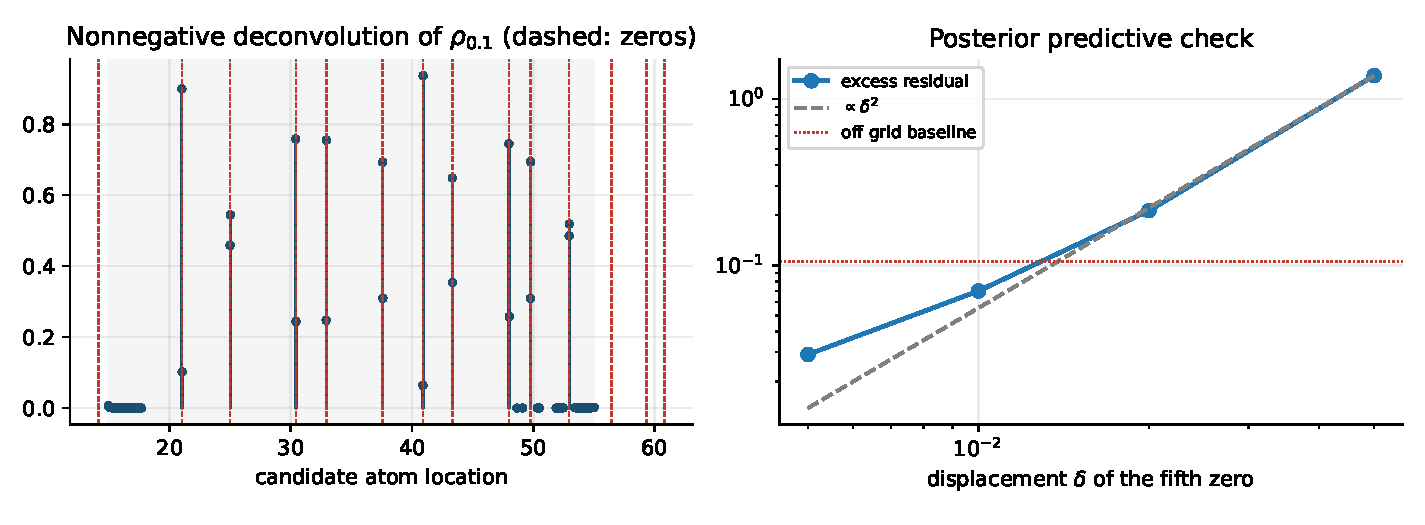
\includegraphics[width=0.95\textwidth]{fig/deconv.pdf}
\caption{Left: the weights of the nonnegative solution for $\rho_{0.1}$ (stems) and the zeros (dashed), with the data window $[15,55]$ shaded. Each zero in the data window carries adjacent weights of total mass one to within half a per cent; the zeros at $14.13$, $56.45$, $59.35$ and $60.83$, outside it, carry none. Right: the excess residual against the displacement $\delta$ of the fifth zero, the $\delta^2$ law through the point at $\delta=0.05$, and the off grid baseline $r_0=0.106$.}
\label{fig:ch17:deconv}
\end{figure}

\subsection{A displaced zero and the threshold of detection}\label{sec:ch17:ppc}

To calibrate the check we displaced the fifth zero, $\gamma_5=32.935$, in the sense of Proposition~\ref{prop:signature}(i): we added to the data the change per displaced zero, $g=\frac12(P_{\varepsilon+\delta}+P_{\varepsilon-\delta})-P_\varepsilon$, centred at $\gamma_5$, and refitted. Twice $g$ is the change in the density when a double zero at $\frac12+i\gamma_5$ leaves the line as the quadruple $\frac12\pm\delta\pm i\gamma_5$, as at a collision in the de Bruijn Newman flow (Section~\ref{ch:dbn}). Table~\ref{tab:ch17:ppc} gives the residuals.

\begin{table}[htbp]
\centering\small
\begin{tabular}{rrrr}
\toprule
$\delta$ & residual $r=\|Aw-y\|$ & excess over baseline & total mass\\
\midrule
0 & 0.1058 & 0 & 10.0942\\
0.005 & 0.1098 & 0.029 & 10.0947\\
0.01 & 0.1269 & 0.070 & 10.0963\\
0.02 & 0.2380 & 0.213 & 10.1031\\
0.05 & 1.3891 & 1.385 & 10.1566\\
\bottomrule
\end{tabular}
\caption{Nonnegative deconvolution of $\rho_{0.1}$ with the signature $g$ of a displaced fifth zero added to the data. Here $r$ is the residual norm and $r_0=0.1058$ its value at $\delta=0$; the excess is $\sqrt{r^2-r_0^2}$.}
\label{tab:ch17:ppc}
\end{table}

For $\delta\ge0.02$ the excess residual grows roughly like $\delta^2$, as the signature does (Proposition~\ref{prop:signature}(i) and \cite[Proposition 19.7]{P26}): it rises from $0.21$ at $\delta=0.02$ to $1.39$ at $\delta=0.05$, a factor $6.5$ for a factor $2.5$ in $\delta$, against $2.5^2=6.25$. At the smallest displacements it grows more slowly, by a factor $2.4$ from $\delta=0.005$ to $0.01$, because there it is dominated by the cross term between the signature and the off grid misfit at $\gamma_5$, which has the same shape. The off grid baseline therefore limits detection: the excess reaches it between $\delta=0.01$ and $0.02$ (Figure~\ref{fig:ch17:deconv}, right). This is the square root law that \eqref{eq:ch8:threshold} states for the matched distance (Section~\ref{sec:ch8:calibration}): since the misfit grows like the square of the displacement, the smallest detectable displacement falls like the square root of the achievable residual, whatever limits the residual. A finer grid of spacing $h$ lowers the baseline like $h^2$ and hence the threshold like $h$, and continuous atom positions would remove the baseline and leave the threshold to the accuracy of the data.

For $\delta\ge\varepsilon$ the check is unreliable. At $\delta=\varepsilon$ the zero $\frac12+\delta+i\gamma_5$ lies on the line of evaluation, where its kernel is a point mass that the samples miss, and the residual, $0.099$, falls below the baseline. For $\delta>\varepsilon$ the atom at $\gamma_5$ leaves the data and is replaced by the signed term $\frac12(P_{\varepsilon+\delta}+P_{\varepsilon-\delta})$ of total mass zero, whose negative part, of mass $\varepsilon/(\pi\delta)+O(\varepsilon^3/\delta^3)$ by Proposition~\ref{prop:signature}(iii), fades as $\delta$ grows. The unit of mass that leaves the data is what the zero density identity of Proposition~\ref{prop:zerodensity} counts, and zeros farther from the line than $\varepsilon$ are left to that identity.

As \cite[Section 19.3.7]{P26} emphasises, this is a model check at finite height and not a route to a proof. What the P\'olya route adds is the small resolution, where the signature $(\delta/\varepsilon)^2$ of Proposition~\ref{prop:signature}(i) is largest for a given $\delta$. The recovery and the calibration are computed, at one resolution and on one window.

The direction of this section is the hard one: Poisson smoothing, which moves the basepoint to the right, preserves positivity, while deconvolution, which moves it back towards the critical line, does not (Section~\ref{ag:sec:exactly}). Chapter~\ref{chap:basepoint} starts instead at the basepoint one, the resolution $\varepsilon=\frac12$ (Section~\ref{ch:basepoint}). At the basepoints between one and the centre, Section~\ref{ch:almost} bounds the mass of the negative part of the split \eqref{ag:eq:split}, the Cauchy kernels of any zeros to the right of the basepoint (Theorem~\ref{ag:thm:almost}), and inserts hypothetical off line zeros into the computed density as this section displaced a zero (Section~\ref{ag:sec:num}).

\section{P\'olya's Bessel function: hitting times, a clock and the flow}\label{ch:biane}

P\'olya replaced the kernel $\Phi$ of \eqref{eq:ch2:Phi} by its asymptote $\Phi^*$ and proved that the transform $\Xi^*$ has only real zeros \cite{Polya} (Section~\ref{fm:sec:simple}). The building block of his proof is the Macdonald function
\begin{equation}\label{eq:biane:P}
P(\theta)=K_{i\theta/2}(2\pi)=\int_{\R}e^{-2\pi\cosh2u}\,e^{i\theta u}\,du,
\end{equation}
which has only real zeros and whose zero counting function has the main term of the Riemann von Mangoldt formula. Biane \cite{Biane09} showed that $\Xi$ and $P$ are Mellin transforms of two Brownian hitting times, and that the Thorin measures of these hitting times are spectral measures of the radial Brownian motions on the unitary group $SU(2)$ and on the hyperbolic space $SL_2(\C)/SU(2)$. This section follows the first author's note on Biane's paper \cite{P26bia}. For $P$ every statement of the Thorin programme is a theorem with an explicit witness: the zeros are the Dirichlet spectrum of a Liouville operator, the reciprocal $K_0(2\pi)/K_{\sqrt u}(2\pi)$ is a GGC whose Thorin atoms are the squared zeros, its clock is the hitting time of an explicit diffusion, and its Poisson trace is completely monotone because it is the trace of a semigroup. The model also marks where the analogy stops: by a theorem of Newman, P\'olya's function has a finite de Bruijn Newman constant, although its zeros show no sign of colliding in the range we compute. Section~\ref{sec:biane:hit} sets out the two hitting times and corrects the constants of Biane's dictionary, Section~\ref{sec:biane:wick} reads the dictionary as a Wick rotation, Sections~\ref{sec:biane:zeros} to \ref{sec:biane:kg} treat the zeros of $P$, the index side clock and a Klein Gordon criterion, Section~\ref{sec:biane:flow} follows the zeros of $P$ and of $\Xi$ under the de Bruijn Newman flow, and Section~\ref{sec:biane:assess} sets the two functions side by side. The complete monotonicity conditions of the Poisson trace, and its comparison with the trace of $P$, are in Section~\ref{sec:biane:cm}. The scripts are \texttt{biane\_polya.py}, \texttt{biane\_clock.py}, \texttt{biane\_flow.py}, \texttt{biane\_traces.py} and \texttt{biane\_figs.py}, and every number below that is not quoted from another section comes from one of them.

\subsection{Two hitting times and Biane's dictionary}\label{sec:biane:hit}

As $u\to\pm\infty$ only the term $n=1$ of \eqref{eq:ch2:Phi} matters, and $\Phi(u)\sim4\pi^2e^{9|u|/2}\exp(-\pi e^{2|u|})$. P\'olya replaced $\Phi$ by the even function with the same asymptotics on both sides,
\begin{gather*}
\Phi^*(u)=8\pi^2\cosh\tfrac{9u}2\,e^{-2\pi\cosh2u},\\
\Xi^*(\theta)=\int_{\R}\Phi^*(u)e^{i\theta u}\,du=4\pi^2\Big[P\big(\theta-\tfrac{9i}2\big)+P\big(\theta+\tfrac{9i}2\big)\Big],
\end{gather*}
since the factor $e^{\pm9u/2}$ shifts the argument of the transform by $\mp\frac{9i}2$. This is the form $G(z+ia)+G(z-ia)$ of P\'olya's Hilfssatz~II (Section~\ref{rz:sec:polya}) with $G=P$ and $a=\frac92$: P\'olya proved that $P$, an entire function of order one, has only real zeros, and the Hilfssatz gives the same for $\Xi^*$. In the index of the Bessel function the shift is $\frac94$, since $P(\theta\mp\frac{9i}2)=K_{i\theta/2\pm9/4}(2\pi)$, which is the form of $\Xi^*$ in Section~\ref{fm:sec:simple}. Figure~\ref{fig:biane:kernels} compares the three kernels. As a pointwise approximation $\Phi^*$ is poor near the origin, $\Phi^*(0)=8\pi^2e^{-2\pi}=0.147447$ against $\Phi(0)=0.893394$, and the kernel $e^{-2\pi\cosh2u}$ of $P$ is narrower still; what the three share is the doubly exponential tail, which governs the zero counting functions. Table~\ref{tab:biane:zeros} lists the zeros below height $60$ and the counts up to height $1000$, computed by \texttt{biane\_polya.py} (the zeros of $\Xi^*$ by sign changes of its transform, those of $P$ from the phase of Proposition~\ref{prop:biane:phase} below).

\begin{figure}[htbp]
\centering
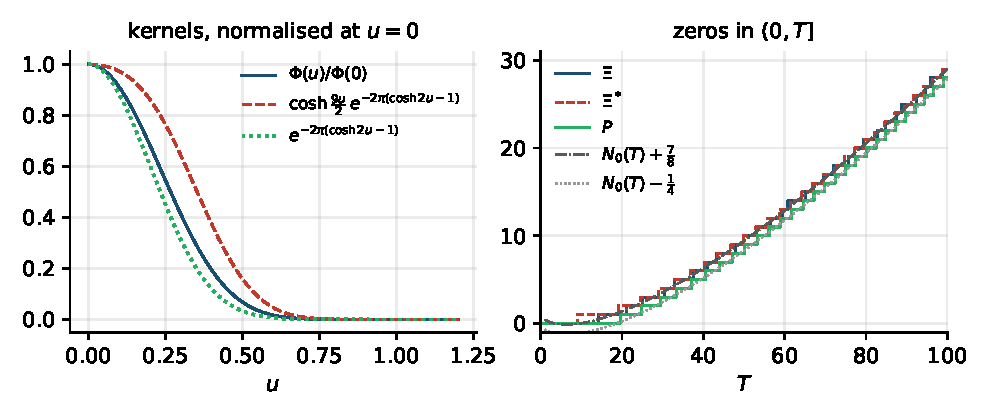
\includegraphics[width=\textwidth]{fig/biane_kernels.pdf}
\caption{Left: the kernel $\Phi$ of \eqref{eq:ch2:Phi}, P\'olya's asymptote $\Phi^*$ and the kernel $e^{-2\pi\cosh2u}$ of $P$, each divided by its value at $u=0$. Right: the zero counting functions of $\Xi$, $\Xi^*$ and $P$ on $(0,100]$, against $N_0(T)+\frac78$ and $N_0(T)-\frac14$, the mean values of the Riemann von Mangoldt formula and of Proposition~\ref{prop:biane:phase}, with $N_0(T)=\frac T{2\pi}\log\frac T{2\pi e}$. Drawn by \texttt{biane\_figs.py} from \texttt{biane\_polya.json}.}
\label{fig:biane:kernels}
\end{figure}

\begin{table}[htbp]
\centering\small
\begin{tabular}{rlll}
\toprule
$n$ & $\Xi$ & $\Xi^*$ & $P$\\
\midrule
1 & 14.135 & 8.993 & 19.538\\
2 & 21.022 & 19.065 & 24.897\\
3 & 25.011 & 24.475 & 29.370\\
4 & 30.425 & 28.975 & 33.383\\
5 & 32.935 & 33.007 & 37.099\\
6 & 37.586 & 36.737 & 40.600\\
7 & 40.919 & 40.249 & 43.936\\
8 & 43.327 & 43.595 & 47.140\\
9 & 48.005 & 46.807 & 50.234\\
10 & 49.774 & 49.908 & 53.236\\
11 & 52.970 & 52.916 & 56.158\\
12 & 56.446 & 55.843 & 59.009\\
13 & 59.347 & 58.700 & \\
\bottomrule
\end{tabular}
\qquad
\begin{tabular}{rrrrr}
\toprule
$T$ & $\Xi$ & $\Xi^*$ & $P$ & $N_0(T)$\\
\midrule
60 & 13 & 13 & 12 & 11.998\\
100 & 29 & 29 & 28 & 28.127\\
240 & 102 & 102 & 101 & 100.946\\
1000 & 649 & 649 & 647 & 647.741\\
\bottomrule
\end{tabular}
\caption{Left: the positive zeros below $60$ of $\Xi$, of P\'olya's $\Xi^*$ and of $P(\theta)=K_{i\theta/2}(2\pi)$. Right: the numbers of zeros in $(0,T]$ against $N_0(T)=\frac T{2\pi}\log\frac T{2\pi e}$. Computed by \texttt{biane\_polya.py}.}
\label{tab:biane:zeros}
\end{table}

The value $2\pi$ of the argument is forced. P\'olya's asymptotics for the zeros of $y\mapsto K_{iy}(2a)$, which Biane derives by stationary phase \cite[Section 3.5]{Biane09}, give $\frac T\pi\log\frac Ta-\frac T\pi+O(1)$ zeros with $0<y\le T$; for $P$ the zeros are at $\theta=2y$ with $a=\pi$, and the count in $(0,T]$ becomes $\frac T{2\pi}\log\frac T{2\pi}-\frac T{2\pi}+O(1)=N_0(T)+O(1)$. The constant $a=\pi$ comes from the factor $e^{-\pi e^{2u}}$ of the term $n=1$, and the $2$ in $\cosh2u$ turns $\frac T\pi\log\frac Ta$ into $\frac T{2\pi}\log\frac T{2\pi}$. Proposition~\ref{prop:biane:phase} gives the counting function of $P$ exactly.

Let $H^{(c)}_a$ be the first passage time of $B_t+ct$ to the level $a>0$, for a standard Brownian motion $B$ and a drift $c\ge0$, as in Appendix~\ref{app:notation}. Its density is $a(2\pi\tau^3)^{-1/2}e^{-(a-c\tau)^2/2\tau}$, the inverse Gaussian law of Table~\ref{tab:ch3:cat}, and its Laplace transform is $e^{a(c-\sqrt{c^2+2u})}$.

\begin{proposition}\label{prop:biane:mellin}
Let $H=H^{(c)}_a$ with $a=c=\sqrt{2\pi}$.
\begin{enumerate}
\item[(i)] $H$ has the density $\tau^{-3/2}e^{2\pi}e^{-\pi(\tau+1/\tau)}$ on $(0,\infty)$, and $1/H$ has the law of $H$ size biased by $H$.
\item[(ii)] $\E H^s=2e^{2\pi}K_{s-\frac12}(2\pi)$ for every $s\in\C$, so that $\E H^s=\E H^{1-s}$.
\item[(iii)] $P(\theta)=\frac12e^{-2\pi}\,\E H^{\frac12+\frac{i\theta}2}$ for every $\theta\in\C$.
\item[(iv)] $U=\frac12\log H$ has the density $2e^{2\pi}e^{-u}e^{-2\pi\cosh2u}$, and the law of $U$ size biased by $e^U$ has the density $e^{-2\pi\cosh2u}/K_0(2\pi)$, whose characteristic function is $P(\theta)/P(0)$.
\end{enumerate}
\end{proposition}

\begin{proof}
(i) With $a=c=\sqrt{2\pi}$, $(a-c\tau)^2/2\tau=\pi(\tau+1/\tau)-2\pi$ and $a/\sqrt{2\pi}=1$. The density of $1/H$ at $\sigma$ is $\sigma^{-2}$ times that of $H$ at $1/\sigma$, which is $\sigma^{-1/2}e^{2\pi}e^{-\pi(\sigma+1/\sigma)}$, that is $\sigma$ times the density of $H$ at $\sigma$; in particular $\E H=1$. (ii) The substitution $\tau=e^w$ and $K_\nu(x)=\int_0^\infty e^{-x\cosh w}\cosh(\nu w)\,dw$ \cite[(10.32.9)]{DLMF} give $\int_0^\infty\tau^{\nu-1}e^{-\pi(\tau+1/\tau)}\,d\tau=2K_\nu(2\pi)$, here with $\nu=s-\frac12$; the integral converges for every complex $\nu$, and $K_\nu=K_{-\nu}$ gives the symmetry. (iii) is (ii) at $s=\frac12+\frac{i\theta}2$. (iv) The substitution $\tau=e^{2u}$ turns the density of (i) into $2e^{2\pi}e^{-3u}e^{-2\pi\cosh2u}e^{2u}$; multiplying by $e^u$ and dividing by $\E H^{1/2}=2e^{2\pi}K_0(2\pi)$ gives the last density, and its characteristic function is $\int e^{-2\pi\cosh2u}e^{i\theta u}du/K_0(2\pi)=P(\theta)/P(0)$ by \eqref{eq:biane:P}.
\end{proof}

The parallel with $\Xi$ is exact. By the identity \eqref{bp:eq:bpy} of Biane, Pitman and Yor \cite{BPY01}, with $V=\frac\pi2S_2$, $2\xi(s)=\E V^{s/2}$, so $\Xi(\theta)=\frac12\E V^{\frac14+\frac{i\theta}2}$, and the kernel is $\Phi(u)=\frac12e^{u/2}f_Y(u)$ with $Y=\frac12\log V$: the P\'olya law of \eqref{eq:ch2:mgf} is the law of $Y$ size biased by $e^{Y/2}$, as the law of (iv) is that of $U$ size biased by $e^U$. On the critical line each function is the Fourier transform, in the logarithm of a hitting time, of the law tilted by a power of that time, and in both cases the evenness of the kernel is a reflection symmetry of the hitting time: $\tau\mapsto1/\tau$ for $H$, which is (i), and the functional equation $\E V^{s/2}=\E V^{(1-s)/2}$ for $V$, which comes from Jacobi's theta transformation. Numerically, \texttt{biane\_polya.py} integrates the density of (i) against $\tau^{\frac12+3.5i}$ and obtains $e^{-2\pi}\E H^{\frac12+3.5i}=7.261817522\times10^{-4}=2P(7)$, with an imaginary part of $2\times10^{-50}$, and it checks $\E S_2^s=2(2/\pi)^s\xi(2s)$, which is \eqref{bp:eq:bpy}, by integrating against the density of $S_2$ at $s=1$, $0.7$ and $\frac12+3i$ (values $0.6666666667$, $0.7384660825$ and $0.1205355309-0.3164244329i$, to ten digits both ways).

Both hitting times are GGCs, with the Thorin measures of Table~\ref{tab:ch3:cat}. For $H^{(c)}_a$ the Thorin measure is $a\,\{\pi\sqrt{2z-c^2}\}^{-1}\mathbf 1_{z>c^2/2}\,dz$, and the L\'evy density, $t^{-1}$ times its Laplace transform, is $a\,e^{-c^2t/2}(2\pi t^3)^{-1/2}$; at $a=c=1$ and $t=0.8$ both expressions give $0.3737294249$. For the Bessel hitting time, $\E e^{-uJ_a}=a\sqrt{2u}/\sinh(a\sqrt{2u})$ with $J_a\overset d=a^2J$, so $J_a+J'_a=a^2S_2$ has Thorin measure $2\sum_{n\ge1}\delta_{\pi^2n^2/2a^2}$ and L\'evy density $2t^{-1}\sum_ne^{-\pi^2n^2t/2a^2}$. The Thorin measure can also be read from the continuation of $\Psi(u)=-\log\E e^{-uX}$ across the cut: integrating the Stieltjes inversion \eqref{eq:ch3:inversion},
\[
U\big((0,z)\big)=\frac1\pi\im\Psi(-z+i0)\qquad(z>0\text{ not an atom}),
\]
because each factor $\log(1+u/w)$ with $w<z$ contributes $i\pi$ at $u=-z+i0$. For $H^{(c)}_a$, $\Psi(-z+i0)=a\big(i\sqrt{2z-c^2}-c\big)$ for $z>\frac{c^2}2$, so $U((0,z))=\frac a\pi\sqrt{2z-c^2}$, which is $0.7117625434$ at $a=c=1$, $z=3$, as the integral of the density gives; for $J_a+J'_a$, $\Psi(-\frac{\lambda^2}2+i0)=2\log\frac{\sin\lambda a}{\lambda a}$, which gains $2\pi i$ each time $\lambda a$ passes a multiple of $\pi$. Biane's dictionary identifies these Thorin measures with spectral measures. In his normalisation \cite[(2.1) to (2.3)]{Biane09} the generator $L_1=\frac12\frac{d^2}{dx^2}$ on $[0,\pi]$ with Dirichlet conditions has the eigenfunctions $\sin(kx)$, $k=1,2,\dots$, with eigenvalues $-\frac{k^2}2$, and the spectral measure $\sigma_1=\frac1\pi\sum_{n\ge1}\delta_{n^2/2}$; the generator $L_2=\frac12\frac{d^2}{dx^2}+\frac d{dx}$ on $[0,\infty)$ with a Dirichlet condition at $0$, selfadjoint in $L^2(e^{2x}dx)$, has the generalised eigenfunctions $e^{-x}\sin(kx)$, $k>0$, with eigenvalues $-\frac{k^2+1}2$, and the spectral measure $\sigma_2(d\lambda)=d\lambda/(\pi\sqrt{2\lambda-1})$ on $\lambda>\frac12$. In the wave number $k$ the two measures are $\frac1\pi$ times counting measure and $\frac1\pi$ times Lebesgue measure.

\begin{theorem}[Biane's dictionary, with corrected constants]\label{thm:biane:dict}
\begin{enumerate}
\item[(i)] The Thorin measure of $J_\pi+J'_\pi=\pi^2S_2$ is $2\pi\sigma_1$.
\item[(ii)] The Thorin measure of $H^{(1)}_1$ is $\sigma_2$.
\item[(iii)] The radial generator $\frac12\frac{d^2}{dx^2}+\cot x\frac d{dx}$ of Brownian motion on the unit sphere $S^3\cong SU(2)$ is the Doob transform of $L_1$ by its ground state $\sin x$, $\sin^{-1}(L_1+\frac12)\sin$, and the radial generator $\frac12\frac{d^2}{dx^2}+\coth x\frac d{dx}$ of Brownian motion on $\mathbb H^3=SL_2(\C)/SU(2)$ is the Doob transform of $L_2$ by the harmonic function $1-e^{-2x}$.
\end{enumerate}
\end{theorem}

\begin{proof}
(i) With $a=\pi$ the atoms $\pi^2n^2/2a^2$ are at $n^2/2$, with mass $2=2\pi\cdot\frac1\pi$. (ii) With $a=c=1$ the density $a\{\pi\sqrt{2z-c^2}\}^{-1}$ on $z>\frac{c^2}2$ is that of $\sigma_2$. (iii) For $f$ smooth, $\frac12(f\sin)''=\sin\cdot(\frac12f''+\cot x\,f'-\frac12f)$, so $\sin^{-1}(L_1+\frac12)(f\sin)=\frac12f''+\cot x\,f'$; and $L_2h=0$ for $h=1-e^{-2x}$, while $h^{-1}L_2(hf)=\frac12f''+(1+h'/h)f'$ with $1+h'/h=1+\frac{2e^{-2x}}{1-e^{-2x}}=\coth x$. The eigenfunctions are checked the same way: $L_2(e^{-x}s)=e^{-x}(\frac12s''-\frac12s)$.
\end{proof}

So Riemann's $\xi$ is attached to the compact group and to discrete spectrum, and P\'olya's $P$ to the hyperbolic space and to continuous spectrum. For P\'olya's function itself the parameters are $a=c=\sqrt{2\pi}$ rather than $a=c=1$; Brownian scaling gives $H^{(c)}_a\overset d=\frac ac\,H^{(\sqrt{ac})}_{\sqrt{ac}}$, so the level and the drift can always be made equal, which is the reciprocal symmetry of Proposition~\ref{prop:biane:mellin}(i), but their common value $\sqrt{ac}$ is $\sqrt{2\pi}$ for $P$ and $1$ in the dictionary. Part~(iii) corrects the direction of the Doob transforms in the note \cite{P26bia}, which has $L_1$ and $L_2$ as the transforms of the radial generators; Biane states them in the direction of (iii) \cite[Section 2.4]{Biane09}.

\begin{remark}[Constants in Biane's paper]\label{rem:biane:slips}
Readers of \cite{Biane09} next to this section should note the following. Biane's $K_\mu(x)=\int_0^\infty t^{\mu-1}e^{-\frac x2(t+t^{-1})}dt$ is twice the standard Macdonald function, and his kernel (3.1) is the $\Phi$ of \eqref{eq:ch2:Phi}; with that kernel $\Xi(z)=2\int_0^\infty\Phi(u)\cos(zu)\,du$ holds for the standard $\xi(s)=\frac12s(s-1)\pi^{-s/2}\Gamma(\frac s2)\zeta(s)$, so the factor $\frac12$ is missing from his displayed definition of $\xi$, and his Mellin formula $\E W_a^s=2(2a^2/\pi)^s\xi(2s)$ also uses the standard $\xi$ (both sides are $\frac23$ at $s=1$, $a=1$). In his Section 4.3 the L\'evy measure of $W_a=J_a+J'_a$ should be $2t^{-1}\sum_ne^{-\pi^2n^2t/2a^2}dt$, with the factor $t^{-1}$ and the $\frac12$ in the exponent, and that of the drifted first passage time should carry the level $x$ as a factor. His Thorin measure (4.1) should have its atoms at $\pi^2n^2/2a^2$, not at $n^2/a^2$; the density (4.2) should be $x\,dc/(\pi\sqrt{2c-a^2})$, which for $x=1$ is his density divided by $\sqrt2$, and the identity offered for it should read $(\pi t)^{-1/2}e^{-a^2t/2}=\int_{a^2/2}^\infty e^{-ct}\,dc/(\pi\sqrt{c-a^2/2})$, with $t$ in place of $t^3$. The measure (2.3) lives on $(\frac12,\infty)$, not on $[1,\infty)$. In Propositions 2.3 and 2.4 the drift and the harmonic function are oriented for the cone opposite to the one stated: with the cone $\{y_1\ge\dots\ge y_n\}$ the drift is $\rho'=(n-1,n-3,\dots,1-n)$ and the positive harmonic function is $\prod_{i<j}(1-e^{-2(y_i-y_j)})=e^{-\langle\rho',y\rangle}\prod_{i<j}2\sinh(y_i-y_j)$; the Vandermonde function $\prod_{i>j}(x_i-x_j)$ of his Proposition 2.1 is reversed in the same way, and is positive on the cone as $\prod_{i<j}(x_i-x_j)$. The eigenvalue of Proposition 2.6 is discussed in Remark~\ref{rem:biane:prop26}. With these corrections the dictionary of his Section 4.5 is the exact statement of Theorem~\ref{thm:biane:dict}.
\end{remark}

\subsection{The Wick rotation and the curvature family}\label{sec:biane:wick}

Biane closes his paper by observing that $\xi$ and P\'olya's function are related, through $SU(2)$ and $SL_2(\C)/SU(2)$, ``in this non obvious way'' \cite[Section 4.5]{Biane09}. The relation is a Wick rotation, the substitution of $iy$ for a real variable $y$ in a function analytic in $y$. In quantum mechanics a state evolves by the unitary group $e^{-itH}$, and Wick's device \cite{Wick54} rotates the time axis, $t=-i\tau$, which turns $e^{-itH}$ into the heat semigroup $e^{-\tau H}$; for $H=-\frac12\Delta+V$ the Feynman Kac formula $e^{-\tau H}f(x)=\E_x[\exp(-\int_0^\tau V(B_s)ds)f(B_\tau)]$ makes Brownian motion the Wick rotated form of quantum mechanics. The rotation keeps the spectrum, an eigenvalue $E$ appearing as a frequency $e^{-iEt}$ on one side and as a decay rate $e^{-E\tau}$ on the other, and it exchanges oscillation and positivity: probability laws, Laplace transforms and completely monotone functions live on the Euclidean side, Fourier transforms and their zeros on the real time side. A Thorin measure is spectral data that can be read on either side. The substitution $y\mapsto iy$ exchanges $\sinh$ and $\sin$, $\cosh$ and $\cos$, and Laplace and Fourier transforms, and through Cartan's duality between a symmetric space $G/K$ of noncompact type and its compact dual $U/K$ it reverses the sign of the curvature. Biane's paper contains the rotation in four places: in space (the sign of the curvature), in the Laplace variable, in time (heat kernels) and in the Mellin index. We take them in turn, after recalling the first part of his paper.

Let $H_n=\{y\in\R^n:\sum_iy_i=0\}$ and $\mathcal C=\{y\in H_n:y_1\ge\dots\ge y_n\}$. Biane describes three matrix valued Brownian motions of type A \cite[Section 2]{Biane09}. For traceless Hermitian Brownian motion the ordered eigenvalues perform Brownian motion in $\mathcal C$ conditioned in Doob's sense never to reach the boundary: the semigroup of Brownian motion killed at $\partial\mathcal C$ is the alternating sum $p^0_t(x,y)=\sum_{w\in S_n}\varepsilon(w)p_t(x,wy)$ (the reflection principle), the Vandermonde product $\prod_{i<j}(y_i-y_j)$ is its positive harmonic function vanishing on $\partial\mathcal C$, and the Doob transform is Dyson's Brownian motion \cite{Dyson62}. For Brownian motion $g_t$ on $SL_n(\C)$, the logarithms of the singular values, the radial part of Brownian motion on $SL_n(\C)/SU(n)$, perform Brownian motion in $\mathcal C$ with generator $\frac12\Delta+\langle\nabla\log\tilde h,\nabla\rangle$, $\tilde h(y)=\prod_{i<j}\sinh(y_i-y_j)$ \cite{JonesOConnell06}, which is Brownian motion with drift $\rho'=(n-1,n-3,\dots,1-n)$, killed at $\partial\mathcal C$, transformed by the harmonic function of Remark~\ref{rem:biane:slips}; here the Martin boundary is large, with a point for each direction in the cone. For Brownian motion on $SU(n)$ the eigenvalues $e^{i\theta_j}$, with $\sum_j\theta_j=0$, live in the alcove $\theta_1\ge\dots\ge\theta_n$, $\theta_1-\theta_n\le2\pi$, a fundamental domain of the affine Weyl group $S_n\ltimes((2\pi\mathbb Z)^n\cap H_n)$; the killed semigroup is the alternating sum over that group, and the eigenvalue process is the Doob transform by the Dirichlet ground state $\prod_{j>k}(e^{i\theta_j}-e^{i\theta_k})$, which is a constant multiple of $\prod_{j<k}\sin\frac{\theta_j-\theta_k}2$ because $\sum_j\theta_j=0$.

The three Doob functions are one function at three values of a curvature parameter. For real $\kappa$ put $s_\kappa(z)=\sin(\sqrt\kappa z)/\sqrt\kappa$, so that $s_{-1}=\sinh$, $s_0(z)=z$ and $s_1=\sin$, and
\[
h_\kappa(y)=\prod_{i<j}s_\kappa(y_i-y_j),\qquad|\rho|^2=\sum_{j=1}^n(n+1-2j)^2=\frac{n(n^2-1)}3 .
\]

\begin{proposition}\label{prop:biane:curv}
For every real $\kappa$ and every $n\ge2$, $\Delta h_\kappa=-\kappa|\rho|^2h_\kappa$ on $H_n$.
\end{proposition}

\begin{proof}
For $\kappa=-1$, write $\prod_{i<j}2\sinh(y_i-y_j)=\prod_{i<j}e^{-(y_i+y_j)}(e^{2y_i}-e^{2y_j})$. The Vandermonde determinant gives $\prod_{i<j}(e^{2y_i}-e^{2y_j})=\det(e^{2(n-j)y_i})$, and on $H_n$ the factor $\prod_{i<j}e^{-(y_i+y_j)}=e^{-(n-1)\sum_iy_i}$ is one, so the exponents $2(n-j)$ may be replaced by $2(n-j)-(n-1)=n+1-2j$: $\prod_{i<j}2\sinh(y_i-y_j)=\sum_{w\in S_n}\varepsilon(w)e^{\langle w\rho',y\rangle}$, the Weyl denominator formula. Each $w\rho'$ lies in $H_n$ and has $|w\rho'|^2=|\rho|^2$, so each exponential is an eigenfunction of the Laplacian of $H_n$ with eigenvalue $|\rho|^2$, and $\Delta h_{-1}=|\rho|^2h_{-1}$. This identity between entire functions of $y\in H_n\otimes\C$ continues analytically. For $\kappa<0$, $h_\kappa(y)$ is a constant times $h_{-1}(\sqrt{-\kappa}\,y)$, and the scaling multiplies the Laplacian by $-\kappa$; for $\kappa>0$, $s_\kappa(z)=\sinh(i\sqrt\kappa z)/(i\sqrt\kappa)$, so $h_\kappa(y)$ is a constant times $h_{-1}(i\sqrt\kappa\,y)$, and the substitution multiplies the Laplacian by $(i\sqrt\kappa)^2=-\kappa$. At $\kappa=0$, $h_0$ is the Vandermonde product, the limit of $h_\kappa$ as $\kappa\to0$, since $s_\kappa(z)=z-\kappa z^3/6+O(\kappa^2)$, and it is harmonic.
\end{proof}

\texttt{biane\_polya.py} checks the proposition with a symbolic Laplacian at random points of $H_n$ for $n=2,3,4$ and $\kappa=-1,0,1$, where $|\rho|^2=2$, $8$, $20$. So Biane's three semigroups are one formula,
\[
q^{(\kappa)}_t(x,y)=\frac{h_\kappa(y)}{h_\kappa(x)}\,e^{\kappa|\rho|^2t/2}\,p^{0}_t(x,y),\qquad\kappa\in\{-1,0,1\},
\]
with generator $\frac12\Delta+\langle\nabla\log h_\kappa,\nabla\rangle$, where $p^0$ is the killed kernel of the chamber $\mathcal C$ for $\kappa\le0$ and of the alcove $\{y_1\ge\dots\ge y_n,\ y_1-y_n\le\pi\}$ for $\kappa=1$; for $\kappa=1$ the coordinates are the half angles $y=\theta/2$, in which $h_1$ is the positive Dirichlet ground state of the alcove. The rotation $y\mapsto iy$ sends $h_\kappa$ to a constant times $h_{-\kappa}$, since $s_\kappa(iz)=is_{-\kappa}(z)$: it exchanges the noncompact and the compact Doob functions, passes through Dyson's Brownian motion at the flat point $\kappa=0$, and reverses the sign of the ground energy, $\frac12\Delta h_\kappa=-\frac\kappa2|\rho|^2h_\kappa$, which is $+\frac12|\rho|^2$ for $SL_n(\C)/SU(n)$ and $-\frac12|\rho|^2=\frac{n-n^3}6$ for $SU(n)$ in the half angles.

\begin{remark}[The eigenvalue of Biane's Proposition 2.6]\label{rem:biane:prop26}
Biane endows the Lie algebra of $SU(n)$ with the form $\langle A,B\rangle=-\operatorname{Tr}(AB)$, in which the angles $\theta_j$ perform standard Brownian motion in $H_n$, and states that the ground state $\prod_{j<k}\sin\frac{\theta_j-\theta_k}2$ has the eigenvalue $\frac{n-n^3}6$ for $\frac12\Delta$ \cite[Proposition 2.6]{Biane09}. By Proposition~\ref{prop:biane:curv} in the half angles, the eigenvalue for $\frac12\Delta_\theta$ is $\frac14\cdot\frac{n-n^3}6=\frac{n-n^3}{24}$; more generally, for the form $-c\operatorname{Tr}(AB)$ it is $\frac{n-n^3}{24c}$. Biane's value holds for $c=\frac14$, that is when the half angles are standard Brownian motion. His rank one discussion uses a third normalisation, $c=\frac12$, in which $SU(2)$ is the unit sphere $S^3$, the angle $x\in[0,\pi]$ has the generator $\frac12\frac{d^2}{dx^2}+\cot x\frac d{dx}$ of Theorem~\ref{thm:biane:dict}(iii), and the ground energy is $\frac{2-8}{12}=-\frac12$. \texttt{biane\_polya.py} confirms $\frac12\Delta_\theta h/h=-\frac14,-1,-\frac52$ for $n=2,3,4$.
\end{remark}

In rank one the curvature family is the radial part of Brownian motion on the three dimensional space form of curvature $\kappa$, with generator $\frac12\frac{d^2}{dx^2}+\sqrt\kappa\cot(\sqrt\kappa x)\frac d{dx}$: the sphere of radius $\kappa^{-1/2}$ for $\kappa>0$, the Bessel process of dimension three for $\kappa=0$, and the hyperbolic space of curvature $\kappa$ for $\kappa<0$. Let $J^{(\kappa)}_a$ be its hitting time of the radius $a$ from the centre, with $a<\pi/\sqrt\kappa$ when $\kappa>0$; then $J^{(0)}_a=J_a$, whose Laplace transform is classical \cite{CiesielskiTaylor62}. For $\kappa<0$ the generator is that of the Bessel process of dimension three with drift $\sqrt{-\kappa}$ \cite[(2.5)]{SalminenVallois07}, the norm of a three dimensional Brownian motion with drift of that length, and the case $\kappa<0$ of the next proposition also follows from the Cameron Martin formula, since for Brownian motion without drift started at the centre the exit place of a ball is uniform and independent of the exit time.

\begin{proposition}\label{prop:biane:skappa}
For $u\ge0$,
\[
\E e^{-uJ^{(\kappa)}_a}=\frac{\sqrt{2u-\kappa}\;s_\kappa(a)}{\sinh\big(a\sqrt{2u-\kappa}\big)},
\]
the Laplace transform of a GGC with Thorin measure $\sum_{n\ge1}\delta_{\pi^2n^2/2a^2-\kappa/2}$. Equivalently, the law of $J^{(\kappa)}_a$ is the exponential tilt $e^{\kappa t/2}\,\Pr(J_a\in dt)/\E e^{\kappa J_a/2}$ of the law of $J_a$.
\end{proposition}

\begin{proof}
The generator is the Doob transform of $\frac12\frac{d^2}{dx^2}$ by $s=s_\kappa$, since $s''=-\kappa s$ gives $s^{-1}(\frac12\frac{d^2}{dx^2}+\frac\kappa2)(sf)=\frac12f''+\frac{s'}sf'$ and $s'/s=\sqrt\kappa\cot(\sqrt\kappa x)$. Hence $f(x)=\sinh(x\sqrt{2u-\kappa})/s_\kappa(x)$ satisfies $\frac12f''+\frac{s'}sf'=s^{-1}(\frac12g''+\frac\kappa2g)=uf$ with $g=\sinh(x\sqrt{2u-\kappa})$, and $f$ is, up to a constant factor, the positive increasing solution that stays bounded at $0$, with $f(0+)=\sqrt{2u-\kappa}$. Hence $\E_xe^{-uJ^{(\kappa)}_a}=f(x)/f(a)$ for $0<x<a$, and letting $x\downarrow0$ gives $\E e^{-uJ^{(\kappa)}_a}=f(0+)/f(a)$, which is the formula; for $\kappa>2u$ the square roots are imaginary and the formula is read through $\sinh(ix)/i=\sin x$. As a function of $u$ the denominator divided by $\sqrt{2u-\kappa}$ is entire of order $\frac12$, with zeros where $a\sqrt{2u-\kappa}=i\pi n$, that is at $u=-(\pi^2n^2/2a^2-\kappa/2)$, all negative under the hypothesis on $a$; Hadamard's product in genus zero gives the Thorin measure. The tilt is the formula at $u-\frac\kappa2$ for $\kappa=0$, divided by its value at $u=0$, since $\sqrt{-\kappa}/\sinh(a\sqrt{-\kappa})=1/s_\kappa(a)$.
\end{proof}

At $u=0.7$, $a=0.9$ and $\kappa=1,-1,\frac13$, \texttt{biane\_polya.py} obtains $0.82508145967889$, $0.84051739205883$ and $0.83070660638487$, each the same from the formula, from the tilt and from the product over the Thorin atoms, and the residual of the differential equation is below $10^{-40}$. Three consequences clarify the dictionary. First, Riemann's clock $J_a+J'_a$ is the flat member $\kappa=0$, and its link with $SU(2)$ in Theorem~\ref{thm:biane:dict} is spectral rather than geometric: the atoms $\pi^2n^2/2a^2$ are the Dirichlet spectrum of $\frac12\frac{d^2}{dx^2}$ on $[0,a]$, which for $a=\pi$ is the spectrum of the radial generator of $SU(2)$ shifted by its ground energy $\frac12$. Second, the hyperbolic member $\kappa=-1$ has the discrete atoms $\pi^2n^2/2a^2+\frac12$; P\'olya's continuous measure comes instead from a first passage over a level on the half line, a Dirichlet problem on $[0,\infty)$ with continuous spectrum. Third, the tilt destroys the reciprocal symmetry of $J_a+J'_a$ that encodes the functional equation. With $W=J^{(\kappa)}_1+J'^{(\kappa)}_1$, the function $(\frac\pi2)^s\E W^s$ equals $2\xi(2s)$ for $\kappa=0$ and is symmetric under $s\mapsto\frac12-s$: it takes the value $0.9963110325$ at both $s=0.1$ and $s=0.4$. For $\kappa=1$ the two values are $1.002917197$ and $1.023703077$. A curvature interpolation between the two clocks must therefore be sought in a class that keeps the symmetry (Question~\ref{q:biane:curv}).

Replacing $u$ by a negative value in $\E e^{-uX}$ continues the transform across the origin, and this is the rotation of the Laplace variable used in the inversion formula above. For the curvature family the reciprocal of the transform becomes, for $u<\frac\kappa2$, the damped sine $\sin(a\sqrt{\kappa-2u})/(\sqrt{\kappa-2u}\,s_\kappa(a))$, whose zeros sit at minus the Thorin atoms and slide with $\kappa$; for the drifted clock the reciprocal $e^{a(\sqrt{c^2+2u}-c)}$ becomes $e^{-ac}e^{ia\sqrt{2|u|-c^2}}$ beyond the branch point $u=-\frac{c^2}2$, which has constant modulus and no zeros. Poles of the transform, which require discrete spectrum, here that of a compact space, give atoms of the Thorin measure; a branch cut gives a density. Figure~\ref{fig:biane:wick} shows both.

\begin{figure}[htbp]
\centering
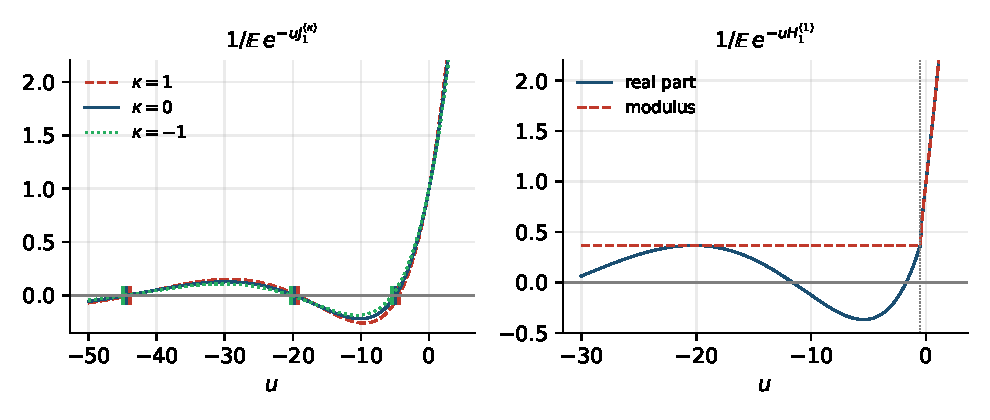
\includegraphics[width=\textwidth]{fig/biane_wick.pdf}
\caption{The Wick rotation of the Laplace variable. Left: $1/\E e^{-uJ^{(\kappa)}_1}$ for $\kappa=1,0,-1$, positive and increasing for $u>0$ and a damped sine for $u<\frac\kappa2$, vanishing at minus the Thorin atoms $\pi^2n^2/2-\kappa/2$ (marks). Right: $1/\E e^{-uH^{(1)}_1}=e^{\sqrt{1+2u}-1}$, real part and modulus; beyond the branch point $u=-\frac12$ (dotted) the modulus is constant, $e^{-1}$, and there are no zeros, the signature of a Thorin density. Drawn by \texttt{biane\_figs.py}.}
\label{fig:biane:wick}
\end{figure}

The rotation of time relates the heat kernels of the two dual spaces. Writing $x=-iy$ gives $\frac d{dx}=i\frac d{dy}$ and $\coth(-iy)=i\cot y$, so $\frac12\frac{d^2}{dx^2}+\coth x\frac d{dx}$ becomes $-(\frac12\frac{d^2}{dy^2}+\cot y\frac d{dy})$, and the Doob functions $\sinh$ and $\sin$ are exchanged. The radial heat kernels of $\frac12\Delta$, relative to the Riemannian volume, are
\begin{gather*}
p^{\mathbb H^3}_t(r)=\frac{e^{-t/2}}{(2\pi t)^{3/2}}\,\frac r{\sinh r}\,e^{-r^2/2t},\\
p^{S^3}_t(\omega)=\frac{e^{t/2}}{(2\pi t)^{3/2}}\sum_{k\in\mathbb Z}\frac{\omega+2\pi k}{\sin\omega}\,e^{-(\omega+2\pi k)^2/2t},
\end{gather*}
and the term $k=0$ of the second is, up to the constant factor $(-1)^{-3/2}$, the first after $r\mapsto i\omega$, $t\mapsto-t$, a genuine Wick rotation of time; the sum over $k$ is the method of images over the affine Weyl group, which makes the kernel periodic. \texttt{biane\_polya.py} checks that both kernels integrate to one against $4\pi\sinh^2r\,dr$ and $4\pi\sin^2\omega\,d\omega$ at $t=0.3$ and $t=1$. In rank $n$ the same statement is the formula for $q^{(\kappa)}_t$, whose factor $e^{\kappa|\rho|^2t/2}$ changes sign with $\kappa$ as $e^{\mp t/2}$ does here. Compactness replaces the continuous spectrum $[\frac12,\infty)$ of $-L_2$ by the lattice $\{\frac{n^2}2\}$ of $-L_1$, which is the passage from $\sigma_2$ to $\sigma_1$ in Theorem~\ref{thm:biane:dict}.

The fourth rotation acts on the Mellin index. The substitution $s=\frac12+i\theta$ turns real Mellin moments into Fourier transforms of a tilted law, and Biane's contour shift $w\mapsto w+\frac{i\pi}2$ \cite[Section 3.5]{Biane09}, with $\cosh(w+\frac{i\pi}2)=i\sinh w$, turns the damped integrand $e^{zw-2a\cosh w}$ into an oscillating one on which stationary phase locates the zeros. For $P$ this is the map $\mu\mapsto i\mu$ on the index of $K_\mu$, and Section~\ref{sec:biane:kg} shows that the index is the eigenvalue of a boost, which the rotation turns into an angular momentum. Table~\ref{tab:biane:wick} collects the dictionary. Atoms of a Thorin measure on the Euclidean side become poles after the rotation, and poles require discrete spectrum, which for these radial Brownian motions, with no potential, means a compact space. That is why $\xi$, whose time side Thorin measure is atomic, is attached to $SU(2)$, while $P$, whose time side measure has a density, is attached to $\mathbb H^3$.

\begin{table}[htbp]
\centering\small
\begin{tabular}{@{}p{0.27\textwidth}p{0.33\textwidth}p{0.33\textwidth}@{}}
\toprule
 & real time side & Euclidean side\\
\midrule
evolution & $e^{-itH}$, oscillating & $e^{-\tau H}$, positive\\
geometry & compact, $S^3=SU(2)$, $\kappa=1$ & noncompact, $\mathbb H^3$, $\kappa=-1$\\
Doob function & $\prod\sin$ & $\prod\sinh$\\
ground energy of $\frac12\Delta$ & $-\frac12|\rho|^2$ & $+\frac12|\rho|^2$\\
radial spectrum & discrete, $\{\frac{n^2}2\}$ & continuous, $[\frac12,\infty)$\\
transform & Fourier, $\E e^{i\lambda X}$ & Laplace, $\E e^{-uX}$\\
Thorin measure & poles and cuts & a positive measure\\
Bessel function & $K_{i\nu}$, oscillating, with zeros & $K_\nu$, positive\\
symmetry of Section~\ref{sec:biane:kg} & boost, rapidity & rotation, angle\\
zeros of $\Xi$ and $P$ & live here & are Thorin atoms here\\
\bottomrule
\end{tabular}
\caption{The two sides of the Wick rotation.}
\label{tab:biane:wick}
\end{table}

\subsection{The zeros of \texorpdfstring{$P$}{P} as a Dirichlet spectrum}\label{sec:biane:zeros}

Put $\psi_\mu(x)=K_\mu(e^x)$. Since $\frac d{dx}=r\frac d{dr}$ for $r=e^x$, the modified Bessel equation $r^2K''+rK'-(r^2+\mu^2)K=0$ becomes
\[
-\psi_\mu''+e^{2x}\psi_\mu=-\mu^2\psi_\mu ,
\]
a Schr\"odinger equation with the Liouville potential $e^{2x}$, in which the index enters only through the energy $-\mu^2$. Let $x_0=\log2\pi$, and let $A_P=-\frac{d^2}{dx^2}+e^{2x}$ act in $L^2([x_0,\infty))$ with a Dirichlet condition at $x_0$. Biane recalls this spectral interpretation of the zeros of the Macdonald function as well known, with Titchmarsh's treatise on eigenfunction expansions \cite{TitchmarshEigen46} as its reference, and notes that P\'olya does not mention it \cite[Section 3.3]{Biane09}. We write $\nu_1<\nu_2<\cdots$ for the positive zeros of $\nu\mapsto K_{i\nu}(2\pi)$, so that $P$ vanishes at $\theta=\pm2\nu_n$.

\begin{proposition}\label{prop:biane:liouville}
\begin{enumerate}
\item[(i)] $A_P$ is selfadjoint, has compact resolvent, and $A_P\ge4\pi^2$.
\item[(ii)] A number $\lambda$ is an eigenvalue of $A_P$ if and only if $\lambda=\nu^2$ with $\nu>0$ and $K_{i\nu}(2\pi)=0$, and the eigenfunction is then $K_{i\nu}(e^x)$. In particular every zero of $P$ is real, of absolute value at least $4\pi$, and the zeros of $P$ are the numbers $\pm2\nu_n$ with $\nu_n^2$ running over the spectrum of $A_P$.
\item[(iii)] Every eigenvalue of $A_P$ is simple, and every zero of $\mu\mapsto K_\mu(2\pi)$ and of $P$ is simple. More precisely, for $\nu>0$ and every $y\in\R$,
\begin{equation}\label{eq:biane:wronski}
\psi_{i\nu}'(y)\,\partial_\nu\psi_{i\nu}(y)-\psi_{i\nu}(y)\,\partial_\nu\psi_{i\nu}'(y)=-2\nu\int_y^\infty\psi_{i\nu}(x)^2\,dx<0 .
\end{equation}
\end{enumerate}
\end{proposition}

\begin{proof}
(i) The endpoint $x_0$ is regular, and the potential is bounded below, so the equation is in the limit point case at $+\infty$ and the Dirichlet realisation is selfadjoint; since $e^{2x}\to\infty$, the resolvent is compact. For $f$ in the form domain, $\langle A_Pf,f\rangle=\int_{x_0}^\infty(|f'|^2+e^{2x}|f|^2)\,dx\ge e^{2x_0}\|f\|^2=4\pi^2\|f\|^2$. (ii) For every complex $\mu$, $K_\mu(r)=\sqrt{\pi/2r}\,e^{-r}(1+O(1/r))$ as $r\to\infty$ \cite[(10.40.2)]{DLMF}, so $\psi_\mu$ is a nonzero solution in $L^2$ near $+\infty$, and in the limit point case it is the only one up to a constant factor. Hence $-\mu^2$ is an eigenvalue exactly when $\psi_\mu(x_0)=K_\mu(2\pi)=0$. By (i) such an eigenvalue is real and at least $4\pi^2$, so $\mu=\pm i\nu$ with $\nu\ge2\pi$; since $P(\theta)=K_{i\theta/2}(2\pi)$, the zeros of $P$ are $\theta=\pm2\nu$. (iii) Two eigenfunctions with the same eigenvalue both vanish at $x_0$, so they are proportional. For \eqref{eq:biane:wronski}, put $\phi=\partial_\nu\psi_{i\nu}$; differentiating $\psi_{i\nu}''=(e^{2x}-\nu^2)\psi_{i\nu}$ in $\nu$ gives $\phi''=(e^{2x}-\nu^2)\phi-2\nu\psi_{i\nu}$, so that $(\psi_{i\nu}'\phi-\psi_{i\nu}\phi')'=2\nu\psi_{i\nu}^2$. Both functions and their derivatives decay like $\exp(-e^x)$, and integrating from $y$ to $\infty$ gives the identity. The function $\psi_{i\nu}$ is real valued and not identically zero, so the right side is negative. At $y=x_0$ and $\nu=\nu_n$ the second term on the left vanishes, so $\partial_\nu K_{i\nu}(2\pi)\ne0$ at $\nu_n$, which is the simplicity of the zero.
\end{proof}

The proposition is P\'olya's theorem that $P$ has only real zeros, obtained from selfadjointness, and $A_P$ is an explicit Hilbert P\'olya operator for $P$. Biane also writes the equation in Dirac form \cite[Section 3.4]{Biane09}. With $D=\frac d{dx}$ and $\mathcal A=D+\frac12+e^x$, whose formal adjoint is $\mathcal A^\dagger=-D+\frac12+e^x$, the system $\mathcal Af=\gamma g$, $\mathcal A^\dagger g=\gamma f$ gives $\mathcal A^\dagger\mathcal Af=\gamma^2f$, and a direct computation gives $\mathcal A^\dagger\mathcal A=A_P+\frac14$. With the Dirichlet condition on $f$ the Dirac eigenvalues are therefore $\gamma=\pm(\nu_n^2+\frac14)^{1/2}$, not $\pm\nu_n$; the shift $\frac14$, which Biane writes as $\gamma^2-\frac14$, is missing from the note \cite{P26bia}. In the variable $u=e^x$ the system reads $(u\frac d{du}+\frac12+u)f=\gamma g$, $(-u\frac d{du}+\frac12+u)g=\gamma f$, and since $u\frac d{du}+\frac12$ is $i$ times the symmetrised dilation operator $\frac12(up+pu)$, $p=-i\frac d{du}$, it is the Hamiltonian $xp$ of Berry and Keating \cite{BerryKeating99} perturbed by the potential $u$, as Biane remarks.

The zeros of $P$ obey an exact quantisation rule. Let $I_\mu$ be the modified Bessel function of the first kind, and for real $\nu$ put
\begin{equation}\label{eq:biane:phase}
\vartheta_P(\nu)=\im\log\Gamma(1+i\nu)-\nu\log\pi-\arg{}_0F_1(;1+i\nu;\pi^2),
\end{equation}
with the branches continuous in $\nu$ and equal to zero at $\nu=0$, where ${}_0F_1(;1;\pi^2)=I_0(2\pi)>0$. Write $N_P(T)$ for the number of zeros of $P$ in $(0,T]$ and
\[
x(T)=\frac1\pi\vartheta_P\big(\tfrac T2\big),\qquad N_0(T)=\frac T{2\pi}\log\frac T{2\pi e}.
\]

\begin{proposition}\label{prop:biane:phase}
\begin{enumerate}
\item[(i)] For $\nu>0$, $I_{i\nu}(2\pi)\ne0$ and
\[
K_{i\nu}(2\pi)=\frac{\pi\,|I_{i\nu}(2\pi)|\,\sin\vartheta_P(\nu)}{\sinh\pi\nu}.
\]
\item[(ii)] $\vartheta_P(\nu)>0$ for $\nu>0$, $\vartheta_P(\nu_n)=n\pi$ for every $n$, and the number of zeros of $\nu\mapsto K_{i\nu}(2\pi)$ in $(0,\nu)$ is $\lceil\vartheta_P(\nu)/\pi\rceil-1$. Equivalently, $N_P(T)=\lfloor x(T)\rfloor$ for every $T>0$ that is not a zero of $P$.
\item[(iii)] As $\nu\to\infty$,
\[
\vartheta_P(\nu)=\nu\log\frac\nu\pi-\nu+\frac\pi4+\frac{\pi^2-\frac1{12}}\nu+O(\nu^{-3}),
\]
so that $x(T)=N_0(T)+\frac14+\big(2\pi-\frac1{6\pi}\big)\frac1T+O(T^{-3})$ as $T\to\infty$.
\end{enumerate}
\end{proposition}

\begin{proof}
(i) For real $r>0$, $I_{-i\nu}(r)=\overline{I_{i\nu}(r)}$, and $K_\mu=\pi(I_{-\mu}-I_\mu)/(2\sin\mu\pi)$ gives $K_{i\nu}(r)=-\pi\im I_{i\nu}(r)/\sinh\pi\nu$. The series $I_{i\nu}(r)=(r/2)^{i\nu}\,{}_0F_1(;1+i\nu;r^2/4)/\Gamma(1+i\nu)$ shows that, for $r>0$,
\[
\vartheta(\nu,r)=\im\log\Gamma(1+i\nu)-\nu\log\frac r2-\arg{}_0F_1\big(;1+i\nu;\tfrac{r^2}4\big)
\]
satisfies $I_{i\nu}(r)=|I_{i\nu}(r)|e^{-i\vartheta(\nu,r)}$, and $\vartheta_P(\nu)=\vartheta(\nu,2\pi)$; this gives the formula. If $I_{i\nu}(r)$ vanished, so would $I_{-i\nu}(r)$, against the Wronskian $I_\mu I_{-\mu}'-I_\mu'I_{-\mu}=-2\sin(\mu\pi)/(\pi r)$ \cite[(10.28.1)]{DLMF}, which is not zero for $\mu=i\nu$. So ${}_0F_1$ does not vanish on $[0,\infty)\times(0,\infty)$, and $\vartheta$ is defined there as a continuous function with $\vartheta(0,r)=0$. (ii) The same Wronskian, written for $I=I_{i\nu}$ and $\bar I=I_{-i\nu}$, gives $\im(I'/I)=\sinh(\pi\nu)/(\pi r|I|^2)$, hence $\partial_r\vartheta(\nu,r)=-\sinh(\pi\nu)/(\pi r|I_{i\nu}(r)|^2)<0$. As $r\to\infty$, $I_{i\nu}(r)\sim e^r/\sqrt{2\pi r}$ and $K_{i\nu}(r)\sim\sqrt{\pi/2r}\,e^{-r}$ uniformly for $\nu$ in compact sets, so $\sin\vartheta(\nu,r)=\sinh(\pi\nu)K_{i\nu}(r)/(\pi|I_{i\nu}(r)|)\to0$ and $\cos\vartheta(\nu,r)>0$ for large $r$; by continuity in $\nu$ from $\nu=0$, $\vartheta(\nu,r)\to0$. So for fixed $\nu>0$ the function $r\mapsto\vartheta(\nu,r)$ decreases from $\vartheta_P(\nu)$ at $r=2\pi$ to $0$ at $r=\infty$; in particular $\vartheta_P(\nu)>0$, and $r\mapsto K_{i\nu}(r)$ has exactly $\lceil\vartheta_P(\nu)/\pi\rceil-1$ zeros in $(2\pi,\infty)$, one at each crossing of a multiple of $\pi$. On the other hand, by \eqref{eq:biane:wronski} at a zero $y$ of $\psi_{i\nu}$, $\psi_{i\nu}'(y)\,\partial_\nu\psi_{i\nu}(y)<0$, so every zero of $x\mapsto K_{i\nu}(e^x)$ moves to the right as $\nu$ increases; no zero comes in from $+\infty$, where $K_{i\nu}(r)>0$ uniformly for $\nu$ in compact sets, and zeros cannot appear in pairs, since they are simple. So the number of zeros in $(x_0,\infty)$ is zero for small $\nu$ and increases by one exactly when $\nu$ passes some $\nu_n$, where a zero enters through $x_0$: it equals the number of $\nu_n<\nu$. Comparing the two counts gives the statement, and $\vartheta_P(\nu_n)\in\pi\mathbb Z$ with the count passing from $n-1$ to $n$ gives $\vartheta_P(\nu_n)=n\pi$. (iii) Stirling's series gives $\im\log\Gamma(1+i\nu)=\nu\log\nu-\nu+\frac\pi4-\frac1{12\nu}+O(\nu^{-3})$, and with $b=1+i\nu$, $\log{}_0F_1(;b;z)=z/b-z^2/(2b^2(b+1))+O(b^{-3})$, so $\arg{}_0F_1(;1+i\nu;\pi^2)=\im\frac{\pi^2}{1+i\nu}+O(\nu^{-3})=-\frac{\pi^2}\nu+O(\nu^{-3})$. With $\nu=T/2$, $\frac1\pi(\nu\log\frac\nu\pi-\nu)=N_0(T)$.
\end{proof}

So the zeros of $P$ are the solutions of $\vartheta_P(\nu_n)=n\pi$, and their counting function is the floor of a smooth function, with no fluctuating remainder. Writing $s_P(T)=\{x(T)\}-\frac12$ for the sawtooth,
\[
N_P(T)=N_0(T)-\frac14-s_P(T)+\Big(2\pi-\frac1{6\pi}\Big)\frac1T+O(T^{-3}),
\]
against the Riemann von Mangoldt formula $N(T)=\vartheta(T)/\pi+1+S(T)$ of Section~\ref{ch:classical}, which with $\vartheta(T)=\frac T2\log\frac T{2\pi}-\frac T2-\frac\pi8+\frac1{48T}+O(T^{-3})$ reads
\[
N(T)=N_0(T)+\frac78+S(T)+\frac1{48\pi T}+O(T^{-3}).
\]
The two counting functions share the main term $N_0$, but their mean constant terms differ by $\frac78+\frac14=\frac98$, and the fluctuation of $N_P$ is the bounded sawtooth of a quantisation rule where that of $N$ is $S(T)$. These two facts govern the comparison of the two Poisson traces in Section~\ref{sec:biane:cm}. Table~\ref{tab:biane:zeros} shows the effect: $N(1000)-N_P(1000)=2$, with $N_0(1000)=647.741$. The note \cite{P26bia} states that the semiclassical count of $A_P$ is exactly the main term of the Riemann von Mangoldt formula. The count is
\[
N_{\rm WKB}(\nu)=\frac1\pi\int_{x_0}^{\log\nu}\sqrt{\nu^2-e^{2x}}\,dx=\frac1\pi\Big(\nu\operatorname{arccosh}\frac\nu{2\pi}-\sqrt{\nu^2-4\pi^2}\Big),
\]
and its expansion gives $N_{\rm WKB}(T/2)=N_0(T)+\frac{2\pi}T+O(T^{-3})$: it agrees with the main term up to $2\pi/T$, not exactly. Its phase $\varphi(\nu)=\pi N_{\rm WKB}(\nu)+\frac\pi4$ is the phase of Debye's expansion of $K_{i\nu}(2\pi)$ for large $\nu$, the term $\frac\pi4$ being the Maslov correction at the turning point, and by (iii) $\vartheta_P(\nu)-\varphi(\nu)=-\frac1{12\nu}+O(\nu^{-3})$.

\texttt{biane\_polya.py} computes $\vartheta_P$ from \eqref{eq:biane:phase} with mpmath at $40$ digits \cite{mpmath} and solves $\vartheta_P(\nu)=n\pi$ by the secant method for every $\nu_n\le1000$, $1516$ zeros. It checks (i) against Arb's $K_{i\nu}(2\pi)$ \cite{Arb} at $\nu=0.5$, $3$, $9.5$, $25$, $101.3$ and $700$, with relative differences below $4\times10^{-37}$, encloses the first $40$ zeros to $10^{-25}$ by sign changes of Arb balls, and finds $137$ sign changes of $K_{i\nu}(2\pi)$ on a grid of step $0.02$ in $(0,150]$, the number of $\nu_n$ below $150$. The first zeros are
\begin{gather*}
\nu_1=9.768770083509978,\qquad\nu_2=12.44848789277578,\\
\nu_3=14.68495977595033,\qquad\nu_4=16.69157893829242,
\end{gather*}
and $\nu_1$ agrees with the first zero of $K_{i\theta}(2\pi)$ in Table~\ref{tab:maxexp:checks}, $9.768770083509977867$. The phase is increasing on $[8,1000]$, where its derivative, sampled with step $0.7$, is at least $0.76$, and the products $\nu(\vartheta_P(\nu)-\nu\log\frac\nu\pi+\nu-\frac\pi4)$ are $9.88388$, $9.79016$ and $9.78643$ at $\nu=20$, $100$ and $500$, against the limit $\pi^2-\frac1{12}=9.78627$ of (iii); the products $\nu(\vartheta_P-\varphi)$ are $-0.1117$, $-0.0843$ and $-0.0834$, against $-\frac1{12}$.

\subsection{The index side: a GGC with the squared zeros as Thorin atoms, and its clock}\label{sec:biane:index}

Biane's Thorin measures in Theorem~\ref{thm:biane:dict} live on the time side: they describe the hitting time itself, in the energy variable of its Laplace transform. The Thorin programme of this book works on the index side, with the reciprocal $1/\E\cosh(\sqrt u\,X)$ of the moment generating function of the P\'olya law, \eqref{eq:ch2:mgf}, whose Thorin atoms would be the squared ordinates. The same hitting time carries both measures, through the Mellin transforms of Proposition~\ref{prop:biane:mellin} and \eqref{bp:eq:bpy}. For P\'olya's function the index side statement is a theorem.

\begin{theorem}\label{thm:biane:indexP}
For $u\ge0$,
\[
\frac{K_0(2\pi)}{K_{\sqrt u}(2\pi)}=\frac{\E H^{1/2}}{\E H^{1/2+\sqrt u}}=\prod_{n\ge1}\Big(1+\frac u{\nu_n^2}\Big)^{-1},
\]
with $H=H^{(\sqrt{2\pi})}_{\sqrt{2\pi}}$ as in Proposition~\ref{prop:biane:mellin}. This is the Laplace transform of the GGC $T_P=\sum_{n\ge1}e_n/\nu_n^2$, with independent standard exponentials $e_n$, no drift and Thorin measure $\sum_n\delta_{\nu_n^2}$.
\end{theorem}

\begin{proof}
$K_\mu(2\pi)=\int_0^\infty e^{-2\pi\cosh t}\cosh(\mu t)\,dt$ is entire and even in $\mu$, so $w\mapsto K_{\sqrt w}(2\pi)$ is entire. Since $|\cosh(\mu t)|\le\cosh(t\re\mu)$, $|K_\mu(x)|\le K_{\re\mu}(x)$, and for $\nu>0$, $K_\nu(x)=\frac12\int_0^\infty s^{\nu-1}e^{-\frac x2(s+1/s)}ds\le\frac12\Gamma(\nu)(2/x)^\nu$. Hence $\log|K_{\sqrt w}(2\pi)|=O(|w|^{1/2}\log|w|)$, the function has order at most $\frac12$ in $w$, and Hadamard's theorem gives a product of genus zero over its zeros. By Proposition~\ref{prop:biane:liouville} these are the points $w=-\nu_n^2$, each simple. So $K_{\sqrt u}(2\pi)=K_0(2\pi)\prod_n(1+u/\nu_n^2)$, and Proposition~\ref{prop:biane:mellin}(ii) with $s=\frac12+\sqrt u$ gives the middle expression. Each factor $(1+u/\nu_n^2)^{-1}$ is the Laplace transform of $e_n/\nu_n^2$, and $\sum_n\nu_n^{-2}<\infty$.
\end{proof}

The theorem is an instance of two results of the book. In the language of Section~\ref{fm:sec:clock}, the law $U$ of Proposition~\ref{prop:biane:mellin}(iv), with density $e^{-2\pi\cosh2u}/K_0(2\pi)$, has the moment generating function $L_U(s)=K_{s/2}(2\pi)/K_0(2\pi)$, which by Proposition~\ref{prop:biane:liouville} vanishes only at $s=\pm2i\nu_n$; so $U$ is ferromagnetic, with $c_k=2\nu_k$ and $b=0$, and Theorem~\ref{fm:thm:dual} gives the clock $T_U=\sum_ke_k/(4\nu_k^2)=T_P/4$, the same variable in the normalisation of the ordinate $\theta$. And Proposition~\ref{rz:prop:lpthorin}, applied to the even function $P$ of order one, which is in the Laguerre P\'olya class by Proposition~\ref{prop:biane:liouville}, gives the GGC $P(0)/P(i\sqrt s)=K_0(2\pi)/K_{\sqrt s/2}(2\pi)$ with atoms at the squared zeros $4\nu_n^2$. For $\Xi$ the corresponding statement is the rigidity theorem, Proposition~\ref{prop:rigid}: $\xi(\frac12)/\xi(\frac12+\sqrt u)$ is a GGC, with Thorin measure $\sum_{\gamma>0}\delta_{\gamma^2}$, if and only if RH holds. For $P$ the equivalence has its hypothesis supplied by selfadjointness, and it comes with an explicit random variable, constructed below. The mean and variance of $T_P$ follow from $K_\mu(x)=k_0(x)+\frac{\mu^2}2k_2(x)+\frac{\mu^4}{24}k_4(x)+\cdots$, with $k_{2j}(x)=\int_0^\infty t^{2j}e^{-x\cosh t}dt$:
\begin{gather*}
\E T_P=\sum_n\frac1{\nu_n^2}=\frac{k_2(2\pi)}{2k_0(2\pi)}=0.0741239453481,\\
\operatorname{Var}T_P=\sum_n\frac1{\nu_n^4}=2.25103144196\times10^{-4},
\end{gather*}
where \texttt{biane\_polya.py} obtains $0.0741239452572$ for the sum over the $1516$ zeros $\nu_n\le1000$ with the tail described next, and the same variance both ways. For comparison, the clock of $\Xi$ has $\E T=0.0231050$ (Section~\ref{ch:clock}).

Table~\ref{tab:biane:products} compares the closed forms with the products over the zeros, for $P$, for P\'olya's $\Xi^*$ and for $\Xi$. The tail beyond the last zero $V$ is $\int_V^\infty\log(1+u/\nu^2)\,dN(\nu)-\frac12\log(1+u/V^2)$, with $dN$ the smooth density of zeros, $\pi^{-1}\vartheta_P'$ from Proposition~\ref{prop:biane:phase}(iii) for $P$ and $\frac1{2\pi}\log\frac T{2\pi}$ for $\Xi^*$ and $\Xi$; the subtracted half term accounts for the last zero sitting at the lower end of the integral. The note \cite{P26bia} truncated at the zeros below a fixed height and continued with the plain density from the last zero; its agreement to three or four digits, which the last column reproduces, is limited by that tail, not by the identities, which hold to the accuracy of the full computation. For $\Xi$ the agreement is a check, not a test, since RH is verified far beyond this range.

\begin{table}[htbp]
\centering\small
\begin{tabular}{llllll}
\toprule
function & $u$ & closed form & product & difference & truncated\\
\midrule
$P$ & $0.5$ & $0.0370339026997$ & $\nu_n\le1000$ & $-4.6\times10^{-11}$ & $1.1\times10^{-5}$\\
 & $2$ & $0.147801988307$ & & $-1.8\times10^{-10}$ & $4.5\times10^{-5}$\\
 & $5$ & $0.367871890035$ & & $-4.6\times10^{-10}$ & $1.1\times10^{-4}$\\
 & $100$ & $6.62276702182$ & & $-9.1\times10^{-9}$ & $2.3\times10^{-3}$\\
$\Xi^*$ & $10$ & $0.3044209914$ & $\gamma^*_n\le1000$ & $1.6\times10^{-8}$ & $8.8\times10^{-5}$\\
 & $60$ & $1.661131318$ & & $9.4\times10^{-8}$ & $5.3\times10^{-4}$\\
 & $200$ & $4.771881099$ & & $3.1\times10^{-7}$ & $1.8\times10^{-3}$\\
$\Xi$ & $10$ & $0.2292377633$ & $1700$ zeros & $1.6\times10^{-7}$ & $3.4\times10^{-5}$\\
 & $60$ & $1.328022599$ & & $9.8\times10^{-7}$ & $2.0\times10^{-4}$\\
 & $200$ & $4.11056511$ & & $3.3\times10^{-6}$ & $6.8\times10^{-4}$\\
\bottomrule
\end{tabular}
\caption[Index side products for $P$, $\Xi^*$ and $\Xi$]{Index side products. The closed forms are $\log(K_{\sqrt u}(2\pi)/K_0(2\pi))$, $\log(\Xi^*(i\sqrt u)/\Xi^*(0))$ and $\log(\xi(\frac12+\sqrt u)/\xi(\frac12))$; the next column says which zeros enter the product $\sum\log(1+u/z^2)$, whose difference from the closed form, after the tail of the text is added, is the fifth column. The last column is the difference for the truncation of the note: the $137$ zeros $\nu_n<150$, the $102$ zeros of $\Xi^*$ below $240$ and $300$ zeros of $\Xi$, each with the plain density from the last zero. Computed by \texttt{biane\_polya.py}.}
\label{tab:biane:products}
\end{table}

P\'olya's $\Xi^*$ belongs to the same class. The law with density proportional to $\Phi^*$ is ferromagnetic (Section~\ref{fm:sec:simple}), so by Theorem~\ref{fm:thm:dual}, or by Proposition~\ref{rz:prop:lpthorin}, $\Xi^*(0)/\Xi^*(i\sqrt u)=\prod_n(1+u/\gamma_n^{*2})^{-1}$ is the Laplace transform of a GGC whose Thorin measure $\sum_n\delta_{\gamma_n^{*2}}$ sits at the squares of the positive zeros $\gamma^*_n$ of $\Xi^*$; the measure is positive. In the language of P\'olya's Hilfssatz~II this is the closure of the class under the cosine tilt: the kernel of $G(\theta+ia)+G(\theta-ia)$ is $2\cosh(au)$ times that of $G$, and P\'olya's passage from $P$ to $\Xi^*$ is this closure with $a=\frac92$ in the variable $\theta$ (Section~\ref{rz:sec:polya}); the note gives the shift as $\frac94$, which is its value in the index of the Bessel function. As a check of the closed form, \texttt{biane\_polya.py} computes $\int\Phi^*(u)\cosh(\sqrt{60}\,u)\,du/\int\Phi^*$ from the kernel and $\Xi^*(i\sqrt{60})/\Xi^*(0)$ from the Bessel functions, and both are $5.265264162$.

The random variable $T_P$ can be realised pathwise. The index of the Bessel equation enters as a centrifugal term $\mu^2/2r^2$, so a Feynman Kac weight $\exp(-\frac u2\int dt/R_t^2)$ along a radial path, the clock of the Hartman Watson law and of Brownian winding, shifts the index from $0$ to $\sqrt u$.

\begin{theorem}\label{thm:biane:clock}
Let $R$ be the diffusion on $(0,\infty)$ with generator
\[
\mathcal G=\frac12\frac{d^2}{dr^2}+\Big(\frac1{2r}-\frac{K_1(r)}{K_0(r)}\Big)\frac d{dr},
\]
the radial part of planar Brownian motion killed at rate $\frac12$ and Doob transformed by $K_0$. For $r>b>0$ let $T_b$ be the hitting time of $b$ and $\tau_r=\frac12\int_0^{T_b}dt/R_t^2$ under $\Pr_r$. Then $T_b<\infty$ almost surely and, for $u\ge0$,
\[
\E e^{-u\tau_r}=\frac{K_{\sqrt u}(r)}{K_0(r)}\cdot\frac{K_0(b)}{K_{\sqrt u}(b)} .
\]
As $r\to\infty$, $\tau_r$ converges in law to $\tau_\infty$ with $\E e^{-u\tau_\infty}=K_0(b)/K_{\sqrt u}(b)$. For $b=2\pi$, $\tau_\infty\overset d=T_P$.
\end{theorem}

\begin{proof}
Let $\mathcal A=\frac12(\frac{d^2}{dr^2}+\frac1r\frac d{dr}-1)$, the generator of the radial part of planar Brownian motion killed at rate $\frac12$. The Bessel equation gives $\mathcal AK_\mu=\frac{\mu^2}{2r^2}K_\mu$, in particular $\mathcal AK_0=0$, and since $K_0'=-K_1$, $\mathcal Gf=K_0^{-1}\mathcal A(K_0f)$. Hence $v=K_{\sqrt u}/K_0$ satisfies $\mathcal Gv=\frac u{2r^2}v$. For real order $K_{\sqrt u}\ge K_0$, so $v\ge1$, and $v(r)\to1$ as $r\to\infty$ because $K_\mu(r)=\sqrt{\pi/2r}\,e^{-r}(1+O(1/r))$ uniformly for bounded $\mu$; so $v$ is bounded on $[b,\infty)$. The scale density of $\mathcal G$ is $s'(r)=1/(rK_0(r)^2)$, which is not integrable at $\infty$, so from $r>b$ the diffusion reaches $b$ before any level $M>r$ with probability $(s(M)-s(r))/(s(M)-s(b))\to1$, and $T_b<\infty$ almost surely; the drift is $-1+\frac1{8r^2}+O(r^{-3})$ at infinity. By It\^o's formula $v(R_{t\wedge T_b})\exp(-\frac u2\int_0^{t\wedge T_b}ds/R_s^2)$ is a bounded martingale, and optional stopping gives $v(b)\E_re^{-u\tau_r}=v(r)$. The limit follows from $v(r)\to1$ and the continuity theorem for Laplace transforms, and the last statement from Theorem~\ref{thm:biane:indexP}.
\end{proof}

In the logarithmic coordinate $X=\log R$, run on the clock $\tau=\frac12\int dt/R_t^2$, It\^o's formula gives
\[
dX_\tau=-2e^{X_\tau}\frac{K_1(e^{X_\tau})}{K_0(e^{X_\tau})}\,d\tau+\sqrt2\,dW_\tau,
\]
a diffusion with generator $\frac{d^2}{dx^2}+2\frac{\psi'}\psi\frac d{dx}=-\psi^{-1}A_P\,\psi$, where $\psi(x)=K_0(e^x)$ is the ground solution of $-\psi''+e^{2x}\psi=0$. Its drift is about $-2e^x$, so $+\infty$ is an entrance boundary, and $\tau_\infty$ is its hitting time of $x_0=\log2\pi$ from $+\infty$. This is the Kent form of Section~\ref{sec:ch18:kent}: by Kent's theorem \cite{Kent80} the hitting time from an entrance boundary is $\sum_ne_n/\lambda_n$ over the Dirichlet eigenvalues $\lambda_n$ of the generator, here those of $A_P$, which are the $\nu_n^2$. For P\'olya's function Theorem~\ref{thm:biane:clock} therefore solves the inverse problem that Sections~\ref{bp:sec:kent} and \ref{sec:ch18:kent} pose for $\xi$: it exhibits the diffusion, here with the Liouville potential, whose hitting time has its Thorin atoms at the squared zeros, without Krein's inverse spectral theory. For $\Xi$ one wants a half line operator with Dirichlet spectrum $\{\gamma^2/4\}$, the counterpart of $\{\nu_n^2\}=\{\theta_n^2/4\}$ over the zeros $\theta_n=2\nu_n$ of $P$; the potential $e^{2x}$ on $[\log2\pi,\infty)$ has the right Weyl law (Proposition~\ref{prop:biane:phase}), so it is the natural reference to perturb, and the perturbation must account for the difference between $\Phi$ and P\'olya's asymptote seen in Figure~\ref{fig:biane:kernels} (Question~\ref{q:biane:radial}).

\begin{corollary}\label{cor:biane:bm}
For real $\lambda$, with $\tau_\infty$ the clock of Theorem~\ref{thm:biane:clock} for $b=2\pi$ and a standard Brownian motion $B$ independent of it,
\[
\frac{K_0(2\pi)}{K_\lambda(2\pi)}=\E e^{i\lambda B_{2\tau_\infty}} .
\]
\end{corollary}

\begin{proof}
$\E e^{i\lambda B_{2\tau}}=\E e^{-\lambda^2\tau}$ for an independent random time $\tau$; apply Theorem~\ref{thm:biane:clock} with $u=\lambda^2$.
\end{proof}

The reciprocal of P\'olya's function along the real axis of the index is thus the characteristic function of Brownian motion run at the index side clock, and the clock is a hitting time of killed planar Brownian motion. For $\Xi$ the corresponding identity $\xi(\frac12)/\xi(\frac12+\lambda)=\E e^{i\lambda B_{2T}}$ holds with no hypothesis, with the clock $T$ of Theorem~\ref{thm:ch12:idsd}, and the variable $B_{2T}$ is the variable $Y_{1/2}$ of Section~\ref{sm:sec:poisson}; what RH adds is that $T$ is the GGC $\sum_\gamma e_\gamma/\gamma^2$ (Proposition~\ref{prop:rigid}). The note \cite{P26bia} states the identity for $\Xi$ under RH and says that for Riemann's function the random time exists if and only if RH holds; the time exists unconditionally, and only its GGC form is equivalent to RH.

\begin{remark}[The Hartman Watson law]\label{rem:biane:hw}
Theorem~\ref{thm:biane:clock} is the $K$ counterpart of a formula of Yor \cite{Yor80} for the Hartman Watson law \cite{HartmanWatson74}: for planar Brownian motion started at distance $r$ from the origin and conditioned on $|B_t|=\rho$, $\E[\exp(-\frac u2\int_0^tds/|B_s|^2)]=I_{\sqrt u}(r\rho/t)/I_0(r\rho/t)$. There the endpoint is fixed and the function is $I$; here the path is killed at rate $\frac12$, transformed by $K_0$ and stopped at a level, and the function is $K$. Pitman and Yor develop the general theory of such Bessel laws \cite{PitmanYor81}.
\end{remark}

\texttt{biane\_clock.py} simulates the clock. With $R_0=2\pi e^{2.5}=76.544867$, so that $X$ starts at $\log2\pi+2.5$ as in the note, the exact law of $\tau_{R_0}$ has, from the expansion of $\log v$ in $u$, mean $0.06763390577$ and standard deviation $0.01499747823$, against $0.07412394535$ and $0.01500343775$ for $\tau_\infty$. The script runs $100000$ paths of the Euler scheme for $X$ with step $\Delta=4\times10^{-6}$, the step of the note, and records two hitting times on the same paths: the plain one, the first step that ends below $\log2\pi$, and one with the Brownian bridge correction, under which a step from $x$ to $x'$, both above the level $\ell=\log2\pi$, crosses it with probability $\exp(-(x-\ell)(x'-\ell)/\Delta)$, the variance of the step being $2\Delta$. The plain scheme overshoots the barrier and is late by about $0.5826\sqrt{2\Delta}/|\beta|$, with $\beta=-13.5317$ the drift at the barrier and $0.5826=-\zeta(\frac12)/\sqrt{2\pi}$ the constant of Broadie, Glasserman and Kou \cite{BGK97}, that is by $1.218\times10^{-4}$. Table~\ref{tab:biane:clock} shows that the plain mean is $2.9$ standard errors late, by $1.39\times10^{-4}$, and that the corrected one agrees with the exact mean. The exact Laplace transform is computed with Arb at $704$ bits, since Arb's $K_\mu(x)$ loses about $2x/\log2$ bits to cancellation, $221$ bits at $x=R_0$, and the exact densities by the fixed Talbot contour \cite{Talbot79,AbateValko04} with $32$ nodes; doubling the nodes changes the density at $0.07$, which is $24.85$, by $2\times10^{-13}$, and the computed densities integrate to $0.9999974$ and $0.9999954$ on $[0.015,0.2]$. Figure~\ref{fig:biane:clock} shows both comparisons. The note's own run, $40000$ plain paths with mean $0.067695\pm0.000075$, is consistent with the exact mean and with the predicted lateness.

\begin{table}[htbp]
\centering\small
\fitwidth{\begin{tabular}{lllll}
\toprule
 & mean & standard deviation & $z$ of the mean & quantiles $0.01$, $0.5$, $0.99$\\
\midrule
exact & $0.0676339$ & $0.0149975$ & & \\
plain Euler & $0.0677726$ & $0.0150584$ & $2.91$ & $0.04190$, $0.06559$, $0.11391$\\
bridge corrected & $0.0676538$ & $0.0150221$ & $0.42$ & $0.04185$, $0.06548$, $0.11364$\\
\midrule
$u$ & $25$ & $100$ & $200$ & $400$\\
\midrule
exact $\E e^{-u\tau_{R_0}}$ & $0.196345$ & $2.54238\times10^{-3}$ & $1.65093\times10^{-5}$ & $2.91684\times10^{-9}$\\
$z$, bridge corrected & $-0.25$ & $0.36$ & $0.72$ & $0.12$\\
$z$, plain Euler & $-2.81$ & $-1.84$ & $-0.76$ & $-0.48$\\
\bottomrule
\end{tabular}}
\caption{The clock from $R_0=2\pi e^{2.5}$: exact moments against $100000$ Euler paths with step $4\times10^{-6}$, with and without the bridge correction, and the Laplace transform, with the $z$ scores $(\text{Monte Carlo}-\text{exact})/\text{standard error}$. The standard error of the mean is $4.75\times10^{-5}$; over $0<u\le400$ the largest $|z|$ of the corrected transform is $0.72$. Computed by \texttt{biane\_clock.py}.}
\label{tab:biane:clock}
\end{table}

\begin{figure}[htbp]
\centering
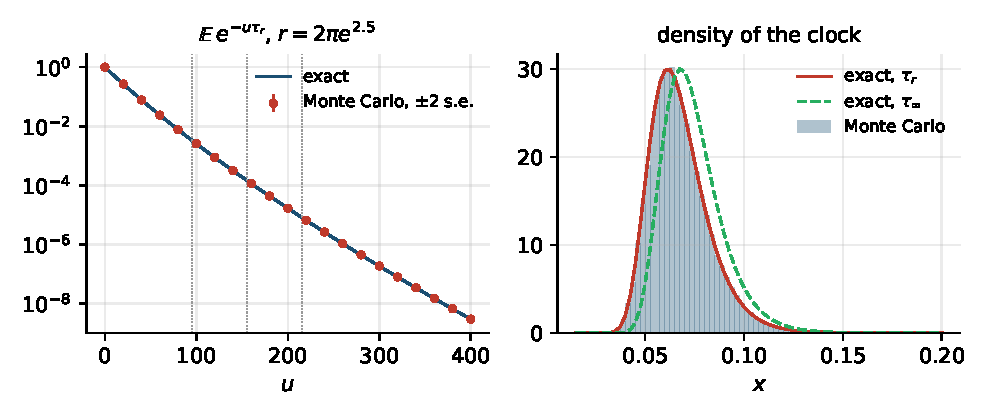
\includegraphics[width=\textwidth]{fig/biane_clock.pdf}
\caption{The clock from $R_0=2\pi e^{2.5}$. Left: $\E e^{-u\tau_{R_0}}$, exact and from the bridge corrected Monte Carlo with two standard errors, on a logarithmic scale; the dotted lines mark the first three Thorin atoms $\nu_1^2=95.4289$, $\nu_2^2=154.965$, $\nu_3^2=215.648$ of $\tau_\infty$. Right: the histogram of the corrected hitting times against the exact densities of $\tau_{R_0}$ and of $\tau_\infty$, by Talbot inversion. Drawn by \texttt{biane\_figs.py} from \texttt{biane\_clock.json}.}
\label{fig:biane:clock}
\end{figure}

The cosine dictionary \eqref{rz:eq:cosdict} turns each Thorin measure of this section into a L\'evy measure of the reciprocal transform, in the variable conjugate to the square root of the energy: a Thorin atom at $z$ becomes the exponential rate $\sqrt z$ when the energy is written $\lambda^2$, and $\sqrt{2z}$ when it is written $\lambda^2/2$, as for Brownian hitting times. Biane's measures give two classical L\'evy measures, and P\'olya's index side measure gives a wave trace.

\begin{proposition}\label{prop:biane:sin2}
For real $\lambda$, $a>0$, $c>0$ and $\ell>0$,
\begin{gather*}
2\log\frac{\sinh\lambda a}{\lambda a}=\int_0^\infty(1-\cos\lambda v)\,\frac{4\,dv}{v\,(e^{\pi v/a}-1)},\\
\ell\big(\sqrt{c^2+\lambda^2}-c\big)=\int_0^\infty(1-\cos\lambda v)\,\frac{2\ell c}\pi K_1(cv)\,\frac{dv}v,\\
\log\frac{K_\lambda(2\pi)}{K_0(2\pi)}=\int_0^\infty4\sin^2\Big(\frac{\lambda v}2\Big)\,\Theta_P(v)\,\frac{dv}v,\qquad\Theta_P(v)=\sum_{n\ge1}e^{-\nu_nv}=\operatorname{tr}e^{-v\sqrt{A_P}} .
\end{gather*}
The left sides are $-\log\E e^{-\lambda^2W/2}$ for $W=J_a+J'_a$ and $W=H^{(c)}_\ell$, and $-\log\E e^{-\lambda^2T_P}$.
\end{proposition}

\begin{proof}
By Frullani's integral, $\log(1+\lambda^2/\beta^2)=\int_0^\infty(1-\cos\lambda v)\,2e^{-\beta v}dv/v$. For $W=J_a+J'_a$ the Thorin measure $2\sum_n\delta_{\pi^2n^2/2a^2}$ of Section~\ref{sec:biane:hit} gives, at $u=\lambda^2/2$, the rates $\beta=\pi n/a$ with weight $2$, and $\sum_ne^{-\pi nv/a}=(e^{\pi v/a}-1)^{-1}$. For $H^{(c)}_\ell$ the density $\ell\{\pi\sqrt{2z-c^2}\}^{-1}$ on $z>\frac{c^2}2$ becomes, under $\beta=\sqrt{2z}$, the measure $\ell\beta\,d\beta/(\pi\sqrt{\beta^2-c^2})$ on $(c,\infty)$, and $\int_c^\infty e^{-\beta v}\beta(\beta^2-c^2)^{-1/2}d\beta=cK_1(cv)$. For $T_P$ take Theorem~\ref{thm:biane:indexP} at $u=\lambda^2$, with rates $\nu_n$, and use $1-\cos=2\sin^2(\cdot/2)$.
\end{proof}

\texttt{biane\_polya.py} checks the first two identities at $\lambda=1.7$, $a=1$, $c=1$, $\ell=0.8$, with the values $0.8845634041934098$ and $0.7778466338652816$ both ways. The Bessel clock has the Planck measure, a geometric superposition of the frequencies $\pi n/a$, and the drifted clock has the Macdonald measure, absolutely continuous because its spectrum is. The dictionary acts on Thorin measures, not on Biane's L\'evy measures in the time variable, which are heat traces. For P\'olya's function the third identity is the exact analogue of the L\'evy Khintchine form of $\xi(\frac12)/\xi(\frac12+u)$ in Section~\ref{sm:sec:poisson}, with the Poisson trace $K_{1/2}$ replaced by the wave trace $\Theta_P$ of the selfadjoint operator $A_P$, which is completely monotone with no hypothesis. In the variable $\theta$, where the zeros of $P$ are $2\nu_n$, the trace is $K^P(y)=\Theta_P(2y)=\sum_ne^{-2\nu_ny}$, and $\log(K_{\lambda/2}(2\pi)/K_0(2\pi))=\int_0^\infty4\sin^2(\lambda y/2)K^P(y)\,dy/y$ has the form of the formula for $\xi$ with $K^P$ in place of $K_{1/2}$; Section~\ref{sec:biane:cm} compares the two traces. At $\lambda=1.7$ the left side of the third identity is $0.2132910704$; the sum over all $1516$ zeros $\nu_n\le1000$ with the tail of Table~\ref{tab:biane:products} differs from it by $3\times10^{-10}$, and the $101$ zeros $\nu_n<120$ with the plain density, as in the note, give $0.2133932327$.

\subsection{Rindler modes and a Klein Gordon criterion}\label{sec:biane:kg}

The clock of Theorem~\ref{thm:biane:clock} lives in the Euclidean plane. Undoing the Wick rotation of the angle gives a Lorentzian picture in which P\'olya's function is a standard object of quantum field theory, and which isolates the structural reason for the reality of its zeros. Put
\[
F(x,w)=\exp(-e^x\cosh w),\qquad\text{so that}\qquad K_\mu(e^x)=\frac12\int_{\R}F(x,w)\,e^{\mu w}\,dw .
\]
Since $\partial_x^2F=(e^{2x}\cosh^2w-e^x\cosh w)F$ and $\partial_w^2F=(e^{2x}\sinh^2w-e^x\cosh w)F$,
\[
\Big(\frac{\partial^2}{\partial x^2}-\frac{\partial^2}{\partial w^2}-e^{2x}\Big)F=0 .
\]
In the coordinates $X_1=e^x\cosh w$, $X_0=e^x\sinh w$ of the Rindler wedge $X_1>|X_0|$, in which $\rho=e^x$ is the proper distance from the edge of the wedge and $w$ the rapidity, $\partial_{X_1}^2-\partial_{X_0}^2=e^{-2x}(\partial_x^2-\partial_w^2)$, so the equation is $(\partial_{X_1}^2-\partial_{X_0}^2-1)F=0$ with $F=e^{-X_1}$: the Klein Gordon equation of unit mass in $1+1$ dimensional Minkowski space, solved by a plane wave. The index $\mu$ is the eigenvalue of the boost generator $\partial_w$, and $K_{i\omega}(\rho)$ is the Rindler mode of boost frequency $\omega$ \cite{Fulling73}. The zeros of $P(\theta)=K_{i\theta/2}(2\pi)$ are therefore, with $\theta=2\omega$, the boost frequencies of the normal modes of a unit mass scalar field in the Rindler wedge with a Dirichlet mirror on the hyperbola $\rho=2\pi$, the configuration of 't Hooft's brick wall model of a black hole horizon \cite{tHooft85}. Biane's Dirac system of Section~\ref{sec:biane:zeros} is the corresponding Dirac field, close to the Rindler space models of Sierra for the Hamiltonian $xp$ \cite{Sierra14}.

The Wick rotation $w=i\phi$ turns the wedge into the Euclidean plane in polar coordinates $(\rho,\phi)$, the boost into a rotation, the Klein Gordon operator into $\Delta-1$, and the plane wave $e^{-X_1}$ into $e^{-\rho\cos\phi}$, which is harmonic for $\frac12(\Delta-1)$, the generator of planar Brownian motion killed at rate $\frac12$ of Theorem~\ref{thm:biane:clock}. The boost frequency becomes the angular momentum $\mu$, and the radial operator $\frac12(\partial_\rho^2+\rho^{-1}\partial_\rho-\mu^2/\rho^2-1)$ carries the index as the centrifugal term that the Feynman Kac weight of the clock produces. The energy of Biane's dictionary, the rapidity of the Rindler picture and the index of the clock are three readings of one rotation, the last row of Table~\ref{tab:biane:wick}. The structure that makes the zeros of $P$ real can be stated for a general even kernel.

\begin{theorem}[A Klein Gordon criterion]\label{thm:biane:kg}
Let $g$ be even, positive and continuous with $\int g(w)e^{c|w|}dw<\infty$ for every $c$, and $G(t)=\int g(w)e^{itw}dw$. Suppose that there are $x_0\in\R$, a real continuous function $V$ on $[x_0,\infty)$ bounded below, and $F\in C^2([x_0,\infty)\times\R)$ such that
\begin{enumerate}
\item[(a)] $(\partial_x^2-\partial_w^2-V(x))F=0$ and $F(x_0,\cdot)=g$;
\item[(b)] $F$ and its partial derivatives of order at most two are $O(e^{-c|w|})$ for every $c>0$, uniformly for $x$ in compact subsets of $[x_0,\infty)$, and $\Psi_\mu(x)=\int F(x,w)e^{\mu w}dw$ lies in $L^2((x_0,\infty))$ for every $\mu\in\C$;
\item[(c)] $\Psi_\mu$ is not identically zero for any $\mu\in\C$.
\end{enumerate}
Then every zero of $G$ is real, and its square is an eigenvalue of $-\frac{d^2}{dx^2}+V$ on $[x_0,\infty)$ with a Dirichlet condition at $x_0$.
\end{theorem}

\begin{proof}
By (b), $\Psi_\mu$ is twice differentiable under the integral sign, and two integrations by parts in $w$, whose boundary terms vanish, give $\Psi_\mu''=\int(\partial_w^2F+VF)e^{\mu w}dw=(\mu^2+V)\Psi_\mu$. Since $V$ is bounded below, the operator $-\frac{d^2}{dx^2}+V$ is in the limit point case at $\infty$, and its Dirichlet realisation at $x_0$ is selfadjoint. If $G(t)=0$, then $\Psi_{it}(x_0)=G(t)=0$ by (a), and by (b) and (c) $\Psi_{it}$ is an eigenfunction with eigenvalue $-(it)^2=t^2$, which is therefore real. So $t$ is real or purely imaginary, and $t=-i\mu$ with real $\mu$ is excluded because $G(-i\mu)=\int g(w)e^{\mu w}dw>0$.
\end{proof}

For P\'olya's function the hypotheses hold in the rapidity variable $w=2u$: with $g(w)=e^{-2\pi\cosh w}$, $G(t)=2K_{it}(2\pi)=2P(2t)$, $V(x)=e^{2x}$, $x_0=\log2\pi$, $F=\exp(-e^x\cosh w)$ and $\Psi_\mu(x)=2K_\mu(e^x)$, and the theorem gives Proposition~\ref{prop:biane:liouville}(ii) again. \texttt{biane\_polya.py} checks the equation for $F$ at $(x,w)=(0.7,0.4)$, with residual $-5.7\times10^{-42}$ at $40$ digits. The criterion says that the reality of the zeros of an even Fourier transform follows from embedding its kernel as the boundary value of a field that satisfies a Klein Gordon equation with a real, time independent potential, which decays fast enough in the rapidity.

For $\Xi$ the corresponding object would be such an extension of $\Phi$, and it would prove RH (Question~\ref{q:biane:kg}). The scaling matters. For $P$ the eigenvalues of $A_P$ are $\nu_n^2=\theta_n^2/4$, and the function whose zeros they are, as a function of the spectral parameter $\mu$ at the boundary $x_0$, is the Jost function $\mu\mapsto\Psi_\mu(x_0)=2K_\mu(2\pi)=2P(-2i\mu)$. A potential asymptotic to $e^{2x}$ at $+\infty$ has the Weyl law of Proposition~\ref{prop:biane:phase}, which matches the zeros of $\Xi$ only in the same scaling, $g(w)=\Phi(w/2)$ and $G(t)=2\Xi(2t)$, and then the Jost function is $\mu\mapsto2\Xi(-2i\mu)=2\xi(\frac12+2\mu)$. The note \cite{P26bia} proposes $\mu\mapsto\xi(\frac12+\mu)$, which corresponds to the eigenvalues $\gamma^2$, whose density is half that of the Weyl law of $e^{2x}$ (a potential growing like $e^{4x}$ would match them). Inverse spectral theory reconstructs an operator from its eigenvalues and norming constants, a potential in the forms of Gelfand and Levitan or of Marchenko and a string in Krein's form, and under RH and the simplicity of the zeros Krein's theory realises the eigenvalues $\gamma^2/4$ (Section~\ref{sec:ch18:kent}); the content of the question is that the operator be of the form $-\frac{d^2}{dx^2}+V$ and that $V$ admit a Klein Gordon solution whose boundary value is $\Phi(w/2)$, which is a statement about the whole function $\xi$ and not only about its zeros.

\subsection{The de Bruijn Newman flow of \texorpdfstring{$P$}{P} against that of \texorpdfstring{$\Xi$}{Xi}}\label{sec:biane:flow}

For real $t$ put
\begin{gather*}
P_t(\theta)=\int_{\R}e^{tu^2/4}e^{-2\pi\cosh2u}\,e^{i\theta u}\,du,\\
\Xi_t(\theta)=\int_{\R}e^{tu^2/4}\,\Phi(u)\cos(\theta u)\,du=8H_t(2\theta),
\end{gather*}
so that $P_0=P$, $\Xi_0=\Xi$, and $t$ is the time of the de Bruijn Newman flow in the normalisation of Section~\ref{sec:ch21:flow}. Decreasing $t$ is the direction in which real zeros can be lost: RH is the statement that $\Xi_t$ keeps only real zeros down to $t=0$, and by the theorem of Rodgers and Tao \cite{RodgersTao} it has nonreal zeros for every $t<0$. For P\'olya's kernel the analogous constant is finite.

\begin{proposition}\label{prop:biane:lambdaP}
There is a constant $\Lambda_P$ with $-\infty<\Lambda_P\le0$ such that $P_t$ has only real zeros if and only if $t\ge\Lambda_P$.
\end{proposition}

\begin{proof}
Let $S$ be the set of $t$ for which $P_t$ has only real zeros. By Proposition~\ref{prop:biane:liouville}, $0\in S$. If $t\in S$ and $t'>t$, then $t'\in S$ by de Bruijn's theorem on the Gaussian factor $e^{\lambda u^2}$, $\lambda>0$ \cite[Theorem~13]{deBruijn}, which applies to the kernel $e^{tu^2/4}e^{-2\pi\cosh2u}$ because it is $O(e^{-|u|^b})$ for every $b>2$. If $t_k\in S$ decrease to $t$, then $P_{t_k}\to P_t$ locally uniformly on $\C$ by dominated convergence, with $|e^{t_ku^2/4}e^{i\theta u}|\le e^{t_1u^2/4}e^{|\im\theta||u|}$, and $P_t(0)>0$, so by Hurwitz's theorem every zero of $P_t$ is a limit of real zeros and $t\in S$. Hence $S=[\Lambda_P,\infty)$ with $\Lambda_P\in[-\infty,0]$. Suppose $\Lambda_P=-\infty$. Then, for the even probability measure $\rho$ with density $e^{-2\pi\cosh2u}/K_0(2\pi)$, the Fourier transform of $e^{\lambda u^2}\rho(du)$ has only real zeros for every real $\lambda$, and by Newman's theorem \cite{Newman1976}, \cite[Theorem 10]{NewmanWu20}, $\rho$ is either $\frac12(\delta_{u_0}+\delta_{-u_0})$ or has a density $Ku^{2m}\exp(-\alpha u^4-\beta u^2)\prod_j(1+u^2/a_j^2)e^{-u^2/a_j^2}$, with $K>0$, $m\ge0$ an integer, $a_j>0$, $\sum_ja_j^{-4}<\infty$, and $\alpha>0$, or $\alpha=0$ and $\beta+\sum_ja_j^{-2}>0$. The inequality $(1+y)e^{-y}\ge e^{-y^2/2}$ for $y\ge0$ bounds such a density below by $Ku^{2m}\exp(-[\alpha+\sum_j\frac1{2a_j^4}]u^4-\beta u^2)$, while $e^{-2\pi\cosh2u}$ decays faster than $e^{-Cu^4}$ for every $C$. This contradiction gives $\Lambda_P>-\infty$.
\end{proof}

The proof is Newman's proof that $\Lambda>-\infty$ \cite{Newman1976}, Theorem~9 of \cite{NewmanWu20}, which uses only the fact that the kernel decays faster than $e^{-Cu^4}$ for every $C$; it applies verbatim to $\Phi^*$, and to every even, positive kernel with that decay whose Fourier transform has only real zeros. The note \cite{P26bia} conjectures $\Lambda_P=-\infty$, on the evidence of the computation below; Proposition~\ref{prop:biane:lambdaP} shows that the conjecture is false. The computation is still informative, because it shows how differently the two flows behave in the range that can be followed.

\texttt{biane\_flow.py} computes both transforms by the trapezoid rule with step $1/250$ on $[0,2]$ at $90$ digits. The kernels are analytic in $|\im u|<\pi/4$ (the kernel of $P_t$ is entire) and below $10^{-68}$ beyond $u=2$, and at $t=0$ the sums reproduce Arb's $K_{i\theta/2}(2\pi)$ at $\theta=10$, $30$, $60$, $90$ and mpmath's $\Xi$ at $\theta=14.134725$, $50$, $90$ with relative errors between $3.5\times10^{-62}$ and $1.4\times10^{-45}$, the largest at $\theta=90$. The real zeros in $(0,90)$ are located by sign changes on a grid of step $0.05$ and refined, for $t=0,-0.5,\dots,-20$ and $t=-21,\dots,-60$. Table~\ref{tab:biane:flow} and Figure~\ref{fig:biane:flow} show the result. The real zeros of $\Xi_t$ in the window fall from $25$ at $t=0$ to $17$ at $t=-2$, $11$ at $t=-4$, $7$ at $t=-8$ and $2$ at $t=-40$, and they are lost in pairs, neighbouring zeros colliding and leaving the axis: the first collisions in the window, as $t$ decreases, are those of the census of Section~\ref{sec:ch21:hankel}, beginning with $(\gamma_{24},\gamma_{25})$ at $t=-1.144$ and height $88.47$ near the top of the window. The pair $(\gamma_4,\gamma_5)=(30.42,32.94)$ has gone by $t=-4$, and the pair $(\gamma_2,\gamma_3)$ by $t=-15$, after which the first zero is isolated. For $P_t$ nothing of the kind occurs down to $t=-60$: every real zero moves monotonically upward, the first from $19.538$ at $t=0$ to $51.881$ at $t=-60$, and the number in the window falls only as zeros leave it through $\theta=90$: from each time of the grid to the next, every zero increases and the count never increases.

\begin{table}[htbp]
\centering\small
\begin{tabular}{rrlrl}
\toprule
$t$ & $P_t$: zeros & first zero & $\Xi_t$: zeros & first zeros\\
\midrule
$0$ & $24$ & $19.538$ & $25$ & $14.135$, $21.022$, $25.011$\\
$-1$ & $23$ & $19.938$ & $25$ & $14.426$, $21.403$, $25.302$\\
$-2$ & $23$ & $20.342$ & $17$ & $14.719$, $21.793$, $25.589$\\
$-4$ & $23$ & $21.163$ & $11$ & $15.311$, $22.600$, $26.144$\\
$-6$ & $23$ & $22.002$ & $9$ & $15.911$, $23.452$, $26.667$\\
$-8$ & $22$ & $22.857$ & $7$ & $16.518$, $24.365$, $27.139$\\
$-10$ & $22$ & $23.730$ & $7$ & $17.133$, $25.378$, $27.518$\\
$-15$ & $21$ & $25.987$ & $5$ & $18.695$, $44.574$, $58.128$\\
$-20$ & $20$ & $28.353$ & $5$ & $20.290$, $46.563$, $60.344$\\
$-25$ & $19$ & $30.832$ & $5$ & $21.911$, $48.426$, $62.880$\\
$-30$ & $18$ & $33.428$ & $3$ & $23.551$, $50.245$, $89.062$\\
$-40$ & $17$ & $38.989$ & $2$ & $26.866$, $53.858$\\
$-50$ & $15$ & $45.098$ & $2$ & $30.202$, $57.488$\\
$-60$ & $13$ & $51.881$ & $2$ & $33.539$, $61.145$\\
\bottomrule
\end{tabular}
\caption{The real zeros in $(0,90)$ of $P_t$ and $\Xi_t$ along the de Bruijn Newman flow: their numbers, the first zero of $P_t$ and the first three of $\Xi_t$. Computed by \texttt{biane\_flow.py}.}
\label{tab:biane:flow}
\end{table}

\begin{figure}[htbp]
\centering
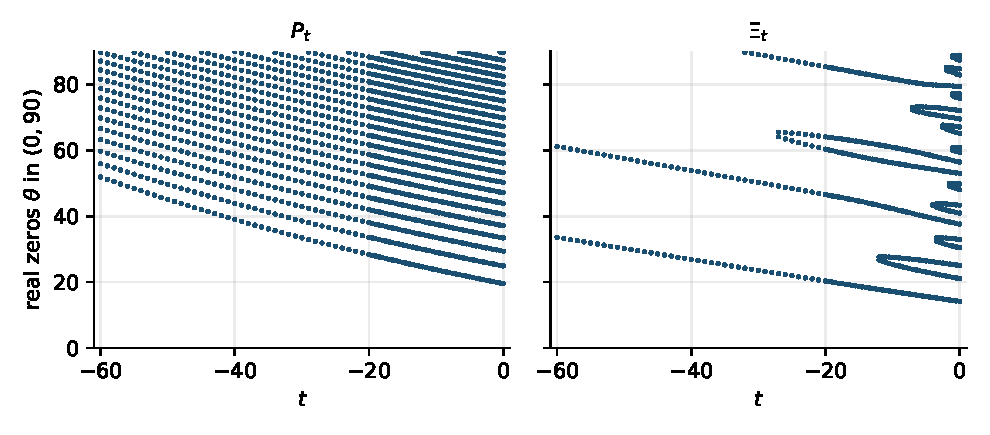
\includegraphics[width=\textwidth]{fig/biane_flow.pdf}
\caption{The real zeros in $(0,90)$ of $P_t$ (left) and of $\Xi_t$ (right) for $-60\le t\le0$, on the grid of Table~\ref{tab:biane:flow} (step $0.5$ above $t=-20$, step $1$ below). The zeros of $P_t$ drift upward and leave the window one at a time; those of $\Xi_t$ collide in pairs. Drawn by \texttt{biane\_figs.py} from \texttt{biane\_flow.json}.}
\label{fig:biane:flow}
\end{figure}

Sign changes count only real zeros, so the script also counts all zeros in the box $0.5\le\re\theta\le60.3$, $|\im\theta|\le3$ by the argument principle, on a contour of step $0.04$ halved wherever the argument changes by more than $0.5$ between neighbours; the largest change that remains is $0.36$. For $P_t$ the box holds $12$, $11$, $8$ and $3$ zeros at $t=0$, $-10$, $-30$ and $-60$, all of them real. For $\Xi_t$ it holds $13$, $12$ and $12$ zeros at $t=0$, $-2$ and $-4$, of which $13$, $10$ and $8$ are real: one conjugate pair has appeared by $t=-2$ and two by $t=-4$. Three of the collisions below height $60$, those listed in the note \cite{P26bia}, are located by bisection in $t$ for the disappearance of two sign changes and then by Newton's method for the double zero $\Xi_t=\partial_\theta\Xi_t=0$ in $(\theta,t)$:
\begin{gather*}
(\gamma_9,\gamma_{10}):\ t_c=-1.877909073,\ \theta_c=49.66423465;\\
(\gamma_4,\gamma_5):\ t_c=-3.954792524,\ \theta_c=33.09873381;\\
(\gamma_2,\gamma_3):\ t_c=-12.49451313,\ \theta_c=27.3212277 .
\end{gather*}
The first agrees with the census of Section~\ref{sec:ch21:hankel} ($-1.87791$ at height $49.664$); the other two lie below its range $[-2.05,0]$. The note presents the three as the first collisions below height $60$, but the computation, on its grid of step $0.5$ in $t$, shows a fourth before $t=-12.5$: the zeros $\gamma_7$ and $\gamma_8$ are at $43.263$ and $43.522$ at $t=-4$ and have left the axis at $t=-4.5$, and the isolated pair estimate of Section~\ref{sec:ch21:flow} puts their collision at about $t=-4.03$, just after that of $(\gamma_4,\gamma_5)$, although they are the closer pair at $t=0$ ($2.408$ apart, against $2.510$). The pair $(\gamma_9,\gamma_{10})$ is the closest pair below height $60$, at distance $1.769$, and its isolated pair estimate $-\frac12(1.769)^2=-1.565$ of Section~\ref{sec:ch21:flow} is again an overestimate of the collision time, the neighbours delaying the collision. In the variable $\theta$ a simple zero moves by
\[
\frac{d\theta_k}{dt}=\frac{\partial_\theta^2F_t(\theta_k)}{4\,\partial_\theta F_t(\theta_k)}=\frac12\sum_{j\ne k}\frac1{\theta_k-\theta_j},
\]
for $F_t=P_t$ and for $F_t=\Xi_t$, which is the equation of motion of Section~\ref{sec:ch21:flow} with $z=2\theta$. At $t=0$ the formula gives $-0.39798088$ for the first zero of $P$ and $-0.28981529$ for the first zero of $\Xi$, and central differences in $t$ with step $10^{-3}$ give the same eight digits. As $t$ decreases every two zeros attract each other, and since the zeros above a given zero are more numerous and denser than those below it, the net pull is upward, which is why both sets of zeros rise; a pair collides when its mutual attraction overcomes the difference of the pulls of all the other zeros on its two members. For $P$ the configuration is regular enough that this does not happen in the window.

The mean motion can be predicted. For $\theta>4\pi$ the integral $P(\theta)$ is dominated by the conjugate saddle points $u_\pm=\pm\frac x2+\frac{i\pi}4$ of $i\theta u-2\pi\cosh2u$, with $x=\operatorname{arccosh}(\theta/4\pi)$, where the exponent is $-\frac{\pi\theta}4\pm i(\frac12\theta x-2\pi\sinh x)$. So $P(\theta)$ is $e^{-\pi\theta/4}$ times a slowly varying amplitude times a cosine of phase $\varphi(\theta)=\frac12\theta x-2\pi\sinh x$ plus a constant; since $\varphi'(\theta)=\frac x2$, the zeros have density $\frac x{2\pi}=\frac1{2\pi}\log\frac\theta{2\pi}+O(\theta^{-2})$. To first order in $t$ the factor $e^{tu^2/4}$ adds to the phase the imaginary part $\frac{\pi t}{16}x$ of $\frac t4u_+^2$, so the number of zeros below a fixed height changes at the rate $\frac x{16}$ per unit of $t$, and each zero moves with
\[
\frac{d\theta}{dt}\approx-\frac{x/16}{x/2\pi}=-\frac\pi8,
\]
whatever its height. The equation of motion gives the same value: with the density $\frac1{2\pi}\log\frac{|\theta|}{2\pi}$ on both half lines, $\frac12\sum_{j\ne k}(\theta_k-\theta_j)^{-1}$ becomes $\frac1{4\pi}$ times the principal value integral of $\log|s|/(\theta_k-s)$, which is $-\frac{\pi^2}2$ for $\theta_k>0$. Over $-0.5\le t\le0$ the $24$ real zeros of $P$ in the window rise at mean speeds that decrease with the height from $0.3990$ (the first zero) to $0.3949$ (the last), towards $\pi/8=0.3927$, while the $25$ zeros of $\Xi$ rise at speeds between $0.0040$, for $\gamma_{25}$, held back by $\gamma_{24}$, which is closing on it, and $0.7350$, for $\gamma_{19}$, which is closing on $\gamma_{20}$, with mean $0.3647$ (\texttt{biane\_figs.py}). The zeros of $P$ move almost as a rigid block; those of $\Xi$ fluctuate about the same mean motion, and the fast and slow members of the close pairs are the ones that collide.

The regularity can be measured. In units of the local mean spacing $2\pi/\log(\theta/2\pi)$, taken at the midpoint of each gap, the smallest gap between consecutive real zeros in the window is
\begin{center}
\small
\begin{tabular}{lllll}
\toprule
$t$ & $0$ & $-10$ & $-30$ & $-60$\\
\midrule
$P_t$ & $1.002$ & $1.020$ & $1.059$ & $1.121$\\
$\Xi_t$ & $0.534$ & $0.490$ & three zeros left & two zeros left\\
\bottomrule
\end{tabular}
\end{center}
(\texttt{biane\_flow.py} and \texttt{biane\_figs.py}). The smallest gap of $P_t$ is always that between the two highest zeros of the window, at almost exactly the mean spacing, and it widens as $t$ decreases, while the smallest gaps of $\Xi_t$, $(59.347,60.832)$ at $t=0$ and $(25.378,27.518)$ at $t=-10$, shrink until the pairs collide. With the density taken at the lower end of each gap, as in the note \cite{P26bia}, the values are $0.968$, $1.014$, $1.053$, $1.115$ for $P_t$ and $0.531$, $0.476$ for $\Xi_t$, and the note's values agree with these to one unit in the third decimal; at $t=0$ the minimum for $P$ then moves to the first gap $(19.538,24.897)$, where the density changes fastest, which is an effect of the convention. The two functions have the same mean density of zeros, $\frac1{2\pi}\log\frac\theta{2\pi}$ (Proposition~\ref{prop:biane:phase}); what differs is the fluctuation, the sawtooth of a quantisation rule for $P$ against $S(T)$ for $\Xi$, whose close pairs (Lehmer pairs, Section~\ref{sec:ch21:collisions}) the flow pushes together.

\begin{remark}[One saddle pair against many]\label{rem:biane:saddle}
For fixed $t$ and large $\theta$ the integral $P_t(\theta)$ is governed by a single pair of complex saddle points of $i\theta u-2\pi\cosh2u+tu^2/4$, conjugate under $u\mapsto-\bar u$ because the kernel is real and even, so that $P_t(\theta)=2\re(Ae^{i\psi_t(\theta)})(1+o(1))$ with a monotone phase, as in P\'olya's asymptotics at $t=0$; heuristically, all but finitely many zeros of $P_t$ are then real for each fixed $t$. For $\Xi_t$ the large $\theta$ asymptotics is the Riemann Siegel expansion, with a number of interfering terms that grows with $\theta$, and the interference is $S(T)$. The note \cite{P26bia} suggests that a version of the saddle point argument uniform in $t$, with a finite computation, would prove $\Lambda_P=-\infty$. By Proposition~\ref{prop:biane:lambdaP} no such uniform version exists: as $t$ decreases below $\Lambda_P$, nonreal zeros appear, outside the box of the argument principle or at times the computation does not reach. The difference between $P$ and $\Xi$ is quantitative, the size of $|\Lambda_P|$ against $\Lambda=0$ under RH, not a difference between a finite and an infinite constant.
\end{remark}

In the language of Lee and Yang \cite{LeeYang} (Section~\ref{rz:sec:polya} and Proposition~\ref{rz:prop:newmanthorin}), the single spin law with density $e^{-2\pi\cosh2u}/K_0(2\pi)$ has the Lee and Yang property, since its moment generating function $K_{h/2}(2\pi)/K_0(2\pi)$ vanishes only at imaginary $h$; it is the ferromagnetic law $U$ of Section~\ref{sec:biane:index}. Newman's theorem says that this property survives every Gaussian factor $e^{-bu^2}$, $b>0$, only for two point laws and for the densities of the proof of Proposition~\ref{prop:biane:lambdaP}, which include the $\varphi^4$ laws $e^{-au^4-bu^2}$ that Simon and Griffiths realised as limits of Ising ferromagnets \cite{SimonGriffiths73}. The law with density proportional to $e^{-2\pi\cosh2u-bu^2}$ has the property exactly when its Fourier transform, a multiple of $P_{-4b}$, has only real zeros, that is when $b\le-\Lambda_P/4$. So the Simon Griffiths type construction for $e^{-2\pi\cosh2u-bu^2}$ at every real $b$ that the note proposes cannot exist.

\subsection{P\'olya's function and \texorpdfstring{$\Xi$}{Xi} side by side}\label{sec:biane:assess}

Table~\ref{tab:biane:compare} sets the two functions side by side. It follows the comparison in the note \cite{P26bia}, corrected in three rows: the index side clock of $\Xi$ exists with no hypothesis, the de Bruijn Newman constant of $P$ is finite, and the computation of the flow describes a window of heights and times, not the whole flow. The Wick rotation of Section~\ref{sec:biane:wick} relates the two entries of each of the second, third and fourth rows. Discreteness moves across the table: $P$ is continuous in the energy and discrete in the angular momentum, while $\Xi$ is discrete in the energy and, under RH, in the angular momentum.

\begin{table}[htbp]
\centering\small
\begin{tabular}{@{}p{0.20\textwidth}p{0.36\textwidth}p{0.36\textwidth}@{}}
\toprule
& P\'olya's $P(\theta)=K_{i\theta/2}(2\pi)$ & Riemann's $\Xi(\theta)$\\
\midrule
kernel & $e^{-2\pi\cosh2u}$, \eqref{eq:biane:P} & $\Phi(u)$, \eqref{eq:ch2:Phi}\\
hitting time & $H^{(\sqrt{2\pi})}_{\sqrt{2\pi}}$, Brownian motion with drift (Proposition~\ref{prop:biane:mellin}) & $\frac\pi2S_2$, three dimensional Bessel process, \eqref{bp:eq:bpy}\\
symmetric space & $\mathbb H^3=SL_2(\C)/SU(2)$ & $SU(2)\cong S^3$\\
Thorin measure of the hitting time (energy) & continuous: $\sigma_2$ for $H^{(1)}_1$ & discrete: $2\pi\sigma_1$ for $\pi^2S_2$ (Theorem~\ref{thm:biane:dict})\\
index side Thorin measure (angular momentum) & $\sum_n\delta_{\nu_n^2}$, a theorem (Theorem~\ref{thm:biane:indexP}) & $\sum_\gamma\delta_{\gamma^2}$ if and only if RH (Proposition~\ref{prop:rigid})\\
index side clock & $\tau_\infty$, a hitting time of an explicit diffusion (Theorem~\ref{thm:biane:clock}) & a random time $T$ (Theorem~\ref{thm:ch12:idsd}); no diffusion is known (Question~\ref{q:biane:radial})\\
trace of the sine squared form & $\Theta_P=\operatorname{tr}e^{-v\sqrt{A_P}}$, completely monotone (Proposition~\ref{prop:biane:sin2}) & $K_{1/2}$, completely monotone if and only if RH (Corollary~\ref{sm:cor:poisson})\\
operator for the zeros & $-\frac{d^2}{dx^2}+e^{2x}$ on $[\log2\pi,\infty)$ (Proposition~\ref{prop:biane:liouville}) & not known\\
Klein Gordon extension & $\exp(-e^x\cosh w)$ (Theorem~\ref{thm:biane:kg}) & not known (Question~\ref{q:biane:kg})\\
de Bruijn Newman constant & $-\infty<\Lambda_P\le0$ (Proposition~\ref{prop:biane:lambdaP}) & $\Lambda\ge0$ \cite{RodgersTao}; RH if and only if $\Lambda=0$\\
real zeros in $(0,90)$ for $-60\le t\le0$ & no collision; mean speeds $0.395$ to $0.399$ on $[-0.5,0]$ & collisions in pairs from $t=-1.144$; mean speeds $0.004$ to $0.735$ on $[-0.5,0]$\\
\bottomrule
\end{tabular}
\caption{P\'olya's function and $\Xi$. Apart from the computations of the last row, the left column is a list of theorems; in the right column the entries that concern the zeros are equivalent to RH or open.}
\label{tab:biane:compare}
\end{table}

The statements about $\Xi$ in the right column and their relatives, Proposition~\ref{prop:rigid}, Corollary~\ref{sm:cor:poisson}, Proposition~\ref{rz:prop:lpthorin} and the GGC form of the clock $T$ discussed after Corollary~\ref{cor:biane:bm}, are proved by Hadamard factorisation, Bernstein's theorem and integral identities. No property of the primes enters their proofs, and none could, since each is an equivalence between two statements about the zeros of one entire function: they reorganise RH, as Section~\ref{ch:open} says of the programme as a whole, and do not approach it. The left column shows that the reorganisation is coherent, since for $P$ every entry is a theorem; but the proofs of the entries on the left that concern the zeros all go through the selfadjoint operator $A_P$, which is exactly what the right column lacks.

The de Bruijn Newman constant explains why a whole family of arguments cannot succeed. The note \cite{P26bia} proves part (a) of the following proposition; part (b) is the strengthening that Newman's theorem gives, and it changes the reading of part (a).

\begin{proposition}\label{prop:biane:damping}
Let $\mathcal P$ be a property of even, positive, integrable kernels such that
\begin{enumerate}
\item[(i)] if $\mathcal P(g)$ holds, then $\int g(u)e^{i\theta u}du$ has only real zeros, and
\item[(ii)] there is $\varepsilon>0$ such that $\mathcal P(g)$ implies $\mathcal P(e^{-\varepsilon u^2/4}g)$.
\end{enumerate}
\begin{enumerate}
\item[(a)] If (ii) holds for $g=\Phi$, then $\mathcal P(\Phi)$ is false.
\item[(b)] If (ii) holds for all $g$ with the same $\varepsilon$, then $\mathcal P(g)$ is false for every kernel $g$ that is $O(e^{-|u|^b})$ for some $b>2$ and satisfies $g(u)e^{Cu^4}\to0$ as $|u|\to\infty$ for every $C$; in particular $\mathcal P$ fails for $\Phi$, for $\Phi^*$ and for $e^{-2\pi\cosh2u}$.
\end{enumerate}
\end{proposition}

\begin{proof}
(a) If $\mathcal P(\Phi)$ held, then by (ii) and (i) the transform of $e^{-\varepsilon u^2/4}\Phi$, which is $\Xi_{-\varepsilon}$ of Section~\ref{sec:biane:flow}, would have only real zeros, so $\Lambda\le-\varepsilon<0$, against the theorem of Rodgers and Tao \cite{RodgersTao}. (b) If $\mathcal P(g)$ held, then by induction $\mathcal P(e^{-k\varepsilon u^2/4}g)$ would hold for $k=0,1,2,\dots$, so the transform of $e^{-k\varepsilon u^2/4}g$ would have only real zeros for each $k$. This kernel is again $O(e^{-|u|^b})$, so by de Bruijn's theorem \cite[Theorem~13]{deBruijn} the transform of $e^{tu^2/4}g$ would have only real zeros for every $t\ge-k\varepsilon$, and hence for every real $t$. By Newman's theorem, as in the proof of Proposition~\ref{prop:biane:lambdaP}, $g/\int g$ would be a density of the form given there, which is bounded below by $Ku^{2m}\exp(-C'u^4-\beta u^2)$ for some $C'$, against the decay of $g$.
\end{proof}

Part (a) uses the theorem of Rodgers and Tao and concerns $\Phi$ alone. Part (b) uses only de Bruijn's theorem and Newman's theorem of 1976, and it shows that the obstruction has nothing to do with the position of $\Phi$ on the boundary of the class of kernels with real zeros: a property that survives a fixed amount of damping for all kernels fails for $P$ as well, although the zeros of $P$ are real for a structural reason, the selfadjointness of $A_P$. So the reading in the note, that P\'olya's kernel tolerates every Gaussian damping, that $P$ has slack and $\Xi$ none, is to be replaced by a quantitative one: $P$ has the finite slack $|\Lambda_P|$, whose size is not known, and $\Xi$ has none if RH holds. Part (b) also limits what the proposition excludes. The note lists among the excluded arguments a ferromagnetic or Lee and Yang construction and a Simon Griffiths representation. The Lee and Yang property of a single spin law is preserved by the ferromagnetic factor $e^{bu^2}$, $b>0$, which runs the flow forward, but by (b) it is not preserved by a fixed damping except on Newman's class. A Lee and Yang representation of the law with density proportional to $\Phi$, which is equivalent to RH (Proposition~\ref{rz:prop:newmanthorin}), is therefore not excluded by the proposition, and neither is a Simon Griffiths type representation of that law. What the proposition excludes is a construction with room to spare, one that would apply to $e^{-\varepsilon u^2/4}\Phi$ as well. The criteria of this section are positivity statements equivalent to RH, of the kind whose history Section~\ref{st:sec:wp5} recalls with the example of Conrey and Li \cite{CL00}; their value here is as a dictionary, not as a plan.

Three questions raised by the note are not equivalences and can be studied without assuming what is to be proved. The first two ask for an object, a diffusion or a potential, not for the zeros, and part (b) does not apply to them, because the existence of such an object is not preserved by a fixed Gaussian damping of every kernel: for $P$ it is lost at every $t<\Lambda_P$, where $P_t$ has nonreal zeros. The third is a question about an explicit kernel with no arithmetic in it, and it measures the slack of P\'olya's function. A fourth concerns the interpolation between the two clocks of Section~\ref{sec:biane:wick}.

\begin{question}\label{q:biane:radial}
Is there a diffusion on a half line, with an entrance boundary, whose hitting time of a level from the entrance boundary has the Laplace transform $\xi(\frac12)/\xi(\frac12+2\sqrt u)$, the transform of the clock $T$ of Theorem~\ref{thm:ch12:idsd} scaled by $4$, as $\tau_\infty$ has the transform $K_0(2\pi)/K_{\sqrt u}(2\pi)$ in Theorem~\ref{thm:biane:clock}? By Kent's theorem \cite{Kent80} such a hitting time is $\sum_ne_n/\lambda_n$ over the Dirichlet eigenvalues $\lambda_n>0$ of the generator, so a positive answer implies RH; under RH and the simplicity of the zeros, Krein's inverse spectral theory gives a generalised diffusion with the eigenvalues $\gamma^2/4$ (Section~\ref{sec:ch18:kent}). The question asks for one constructed without RH, for example as a perturbation of the diffusion $X$ of Section~\ref{sec:biane:index}, whose potential $e^{2x}$ has the right Weyl law.
\end{question}

\begin{question}\label{q:biane:kg}
Does $g(w)=\Phi(w/2)$ admit a Klein Gordon extension in the sense of Theorem~\ref{thm:biane:kg}, with a real potential $V$ asymptotic to $e^{2x}$ at $+\infty$? By the theorem a positive answer implies RH. Under RH the question asks whether $\mu\mapsto2\xi(\frac12+2\mu)$ is, up to normalisation, the Jost function of such a potential whose Klein Gordon solution has the boundary value $g$. A first numerical step is to reconstruct a potential from the first few thousand ordinates and a choice of norming constants by the method of Gelfand and Levitan or of Marchenko, and to test whether it is stable under truncation and close to $e^{2x}$.
\end{question}

\begin{question}\label{q:biane:lambda}
What is the de Bruijn Newman constant $\Lambda_P$ of P\'olya's function, and that of $\Xi^*$, which is also finite and at most $0$ by the proof of Proposition~\ref{prop:biane:lambdaP}? At what height do the first nonreal zeros of $P_t$ appear as $t$ decreases through $\Lambda_P$, and do they appear, as for $\Xi_t$, through the collision of two real zeros?
\end{question}

\begin{question}\label{q:biane:curv}
Is there a one parameter family of laws joining the drifted first passage time and the sum of two Bessel hitting times, each with a reciprocal symmetry that encodes a functional equation, as $\tau\mapsto1/\tau$ does for $H$ in Proposition~\ref{prop:biane:mellin}(i) and Jacobi's transformation does for $S_2$, along which the index side Thorin measure can be followed? The curvature family of Proposition~\ref{prop:biane:skappa} is an Esscher tilt and breaks the symmetry. Positivity of the index side Thorin measure at the Bessel end is RH.
\end{question}

\section{Exercises}\label{chap:probability:ex}

\paragraph{On Section~\ref{ch:clocklaw}.}
\begin{exercises}
\item\label{ex:ch18:residues} Assuming that the zeros are on the critical line and simple, show that the residues of the clock transform at $u=-\gamma_k^2$ are $R_k=2i\gamma_k\xi(\frac12)/\xi'(\frac12+i\gamma_k)$ and that they alternate in sign. (They are the coefficients $c_n$ of Theorem~\ref{bs:thm:nb}.)
\item\label{ex:ch18:origin} Explain why the spectral expansion of the density diverges at $t=0$ while the Talbot inversion does not, and compare the abscissa of convergence in Theorem~\ref{bs:thm:nb}.
\item\label{ex:ch18:hazard} Show that the hazard of a finite sum of exponentials with rates $\lambda_1<\lambda_2<\cdots$ tends to $\lambda_1$ and that $h(t)-\lambda_1$ decays like $e^{-(\lambda_2-\lambda_1)t}$.
\item Sample Williams' variable with $10^5$ draws and estimate $\Xi(5)$; compare the standard error with Table~\ref{tab:ch18:mc}.
\item\label{ex:ch18:floor} Assume RH, let $\Theta_N$ be the cutoff of Section~\ref{sec:ch18:kent}, and assume that $S(\Theta_N)=0$, as for the values of $N$ used there. Show that $\log G(w)-\log G_N^{\rm W}(w)$ tends to $\ell_N=2\int_{\Theta_N}^\infty S(\gamma)\gamma^{-1}\,d\gamma$ as $w\to\infty$. Then, using Stirling's formula for $\log\xi(\frac12+x)$ as $x\to+\infty$ and $\int_0^\infty\log(1+x^2/t^2)\log\frac t{2\pi}\,dt=\pi x\log\frac x{2\pi}-\pi x$, show that
\begin{multline*}
\ell_N=2\sum_{k\le N}\log\gamma_k-\log\xi(\tfrac12)+\tfrac14\log\tfrac\pi2-\frac1\pi\int_0^{\Theta_N}\log t\,\log\frac t{2\pi}\,dt\\
+\frac2\pi\int_{\Theta_N}^\infty\Big(\vartheta'(t)-\frac12\log\frac t{2\pi}\Big)\log t\,dt,
\end{multline*}
the terms in $\log x$ cancelling because $\vartheta(\Theta_N)=(N-1)\pi$. So $\ell_N$ is determined by $\gamma_1,\dots,\gamma_N$ and $\xi(\frac12)$.
\end{exercises}

\paragraph{On Section~\ref{ch:boundaries}.}
\begin{exercises}
\item Show that on the parabola $u=\frac12(-q^2+2icq)$ one has $\re\sqrt{c^2+2u}=c$, and hence that every mixture of inverse Gaussian laws with drift $c$ has transform bounded by one there.
\item Derive the small $q$ expansion $|G(u)|^2=1-q^2(\E T-c^2\mathrm{Var}\,T)+O(q^3)$ on the parabola.
\item\label{ex:ch19:ig} Show that the hazard of the first passage time of Brownian motion across the line $\alpha+\beta t$, with $\alpha>0$ and $\beta<0$, which has the inverse Gaussian law with drift $|\beta|$, tends to $\beta^2/2$ with correction $3/(2t)$.
\item Implement the tangent boundary ODE with a different starting time and check that the asymptotic slope is unchanged.
\item\label{ex:ch19:density} Show that the density $f$ of the clock is continuous and positive on $(0,\infty)$. (The Laplace transform of $T$ equals $1/G$ on $\re u\ge0$, by analytic continuation from $(0,\infty)$ and continuity, so the characteristic function is $1/G(-iy)$; Stirling's formula and the bound $|\zeta(s)|\ge1/\zeta(\re s)$ for $\re s>1$, applied on the rays $\frac12+re^{\pm i\pi/4}$, show that it decays faster than any power of $|y|$. Next, $\log G(u)=o(u)$ as $u\to\infty$, so $P(T<t)>0$ for every $t>0$; $1/G$ has poles, so the law of $T$ has unbounded support; and the law is unimodal by Corollary~\ref{sb:cor:unimodal}, so $f$ itself, which is the derivative of the distribution function at every point, is nondecreasing up to a mode and nonincreasing after it.)
\end{exercises}

\paragraph{On Section~\ref{ch:li}.}
\begin{exercises}
\item Derive formula \eqref{eq:ch20:li} from the derivative representation of $\lambda_n$.
\item Show that $\lambda_1=\sum_\rho\rho^{-1}=1+\frac{\gamma_E}2-\frac12\log4\pi$, and that under RH $\lambda_1=\sum_{\gamma>0}(\gamma^2+\frac14)^{-1}$.
\item Show that under RH $\lambda_n=\sum_{\gamma>0}4\sin^2(n\arctan\frac1{2\gamma})$, and that the terms are of order $n^2/\gamma^2$ for $\gamma\gg n$.
\item\label{ex:ch20:offline} For a hypothetical zero $\rho=\frac12+d+i\gamma$ with $d>0$, show that $|1-1/(1-\bar\rho)|>1$, and estimate the index $n$ at which its contribution would make $\lambda_n$ negative.
\end{exercises}

\paragraph{On Section~\ref{ch:dbn}.}
\begin{exercises}
\item\label{ex:ch21:motion} Show that $H_t$ satisfies $\partial_tH_t=-\partial_z^2H_t$ and derive the equation of motion of a simple zero.
\item For an isolated pair at distance $D_0$, solve $dD/dt=4/D$ and find the collision time.
\item Modify the P\'olya evaluator to compute $H_t$ and reproduce Table~\ref{tab:ch21:traj}.
\item Explain why the collision time of a pair of zeros gives numerical evidence for, but not a proof of, a lower bound on $\Lambda$.
\end{exercises}

\paragraph{On Section~\ref{sec:dbeta:beta}.}
\begin{exercises}
\item Show that $K_4(u)=2e^{3u/2}\eta(ie^{2u})^3$ is even, using $\eta(i/x)=\sqrt x\,\eta(ix)$, and deduce the functional equation $\xi(s,\chi_4)=\xi(1-s,\chi_4)$ from $\xi(\frac12+s,\chi_4)=\int_{\R}K_4(u)e^{su}\,du$.
\item Show that for real $\sigma>0$ the series $\sum_{n\ge0}(-1)^n(2n+1)^{-\sigma}$ lies between $1-3^{-\sigma}$ and $1$, and deduce that $L(s,\chi_4)$ has no zeros on $(0,1)$ without using the kernel.
\item For $0<\varepsilon<\delta$ show that $\pi(P_{\varepsilon+\delta}+P_{\varepsilon-\delta})$ integrates over the interval $|x|<\sqrt{\delta^2-\varepsilon^2}$, where it is negative, to $\pi-4\arctan\sqrt{(\delta+\varepsilon)/(\delta-\varepsilon)}$, which lies in $(-\pi,0)$ and tends to $0$ as $\varepsilon/\delta\to0$; this is the bound on the fall of the argument after Corollary~\ref{cor:dbeta:argmono}.
\item Show that $g(c,u)=2c(3u^2-c^2)/(c^2+u^2)^3$, the second derivative of $c/(c^2+u^2)$ in $u$, has $\partial_cg(c,u)=6(u^4-6c^2u^2+c^4)/(c^2+u^2)^4$, which is positive exactly when $|c|<(\sqrt2-1)|u|$ or $|c|>(\sqrt2+1)|u|$, and deduce that $g(a+\delta,u)+g(a-\delta,u)>0$ for $a,\delta>0$ with $a+\delta<(\sqrt2-1)|u|$, the step for the zeros off the line in the proof of Theorem~\ref{thm:dbeta:minall}(ii).
\end{exercises}

\paragraph{On Section~\ref{ch:biane}.}
\begin{exercises}
\item Show that $1/H$ has the law of $H$ size biased by $H$, for $H=H^{(\sqrt{2\pi})}_{\sqrt{2\pi}}$ with the density of Proposition~\ref{prop:biane:mellin}(i), and deduce $\E H^s=\E H^{1-s}$ without computing the Mellin transform.
\item Show that $F(x,w)=\exp(-e^x\cosh w)$ satisfies $(\partial_x^2-\partial_w^2-e^{2x})F=0$, and that in the coordinates $X_1=e^x\cosh w$, $X_0=e^x\sinh w$ one has $\partial_x^2-\partial_w^2=e^{2x}(\partial_{X_1}^2-\partial_{X_0}^2)$, so that $F=e^{-X_1}$ solves the Klein Gordon equation of unit mass.
\item Show that $(1+y)e^{-y}\ge e^{-y^2/2}$ for $y\ge0$, and deduce that each density of Newman's theorem in the proof of Proposition~\ref{prop:biane:lambdaP} is bounded below by $Ku^{2m}\exp(-[\alpha+\sum_j\frac1{2a_j^4}]u^4-\beta u^2)$.
\item Show that the principal value integral of $\log|s|/(1-s)$ over $\R$, taken with symmetric limits at $\pm\infty$, is $-\frac{\pi^2}2$, and deduce the mean speed $-\frac\pi8$ of the zeros under the flow in Section~\ref{sec:biane:flow} from the density $\frac1{2\pi}\log\frac{|\theta|}{2\pi}$.
\item For $0<y<\pi$ show, as claimed in Subsection~\ref{sec:biane:cm}, that $\gamma^ne^{-\gamma y}$, for $\gamma\le n/\pi$, is at most $\exp(n(\log\frac y\pi+1-\frac y\pi))$ times its maximum over $\gamma>0$, and evaluate the exponent for $n=10^6$ at $y=1$ and at $y=3$.
\end{exercises}

\chapter{The basepoint one}\label{chap:basepoint}

Section~\ref{ch:deconv} recovered the zeros from the Thorin density at the resolution $\varepsilon=0.1$, close to the critical line, where the positivity of the density at every height is open. We now work at the resolution $\varepsilon=\frac12$ of the Cauchy flow $\varepsilon\mapsto\rho_\varepsilon$ of Section~\ref{ch:clock}, the basepoint one. The completed zeta function has two probabilistic readings. On the Mellin side, Williams \cite{Williams90} and Biane, Pitman and Yor \cite{BPY01} showed that $2\xi(s)$ is the Mellin transform of a sum of two Bessel hitting times, which gives the P\'olya variable and its exponential tilts at every basepoint with no hypothesis. On the Laplace side, the shifted clocks $T_\alpha$, with $\E e^{-uT_\alpha}=\xi(\alpha)/\xi(\alpha+\sqrt u)$, carry the Thorin programme. At the centre, $\alpha=\frac12$, the shifted clock is the clock of \cite{P17}, which is infinitely divisible and self decomposable with no hypothesis (Theorem~\ref{thm:ch12:idsd}) and a generalised gamma convolution exactly when RH holds (Proposition~\ref{prop:rigid}). At a basepoint $\alpha$ to the right of every zero, $T_\alpha$ is a GGC whose Thorin density is the Poisson smoothing of the zeros by Cauchy kernels of widths $\alpha-\beta$ (Theorem~\ref{thm:poisson} and Proposition~\ref{prop:struct}), and from $\alpha=1$ on this density is positive with no hypothesis, because no zero lies on the line $\re s=1$ or to its right. The basepoint one is therefore the leftmost basepoint at which positivity is a theorem, and the natural place to separate what is unconditional from what is equivalent to RH.

At the basepoint one everything can be computed and most things can be proved, and we work the example out completely, as a test bed for the tools of the book. We ask three questions of $T_1$: what its Thorin measure and its law are, whether its Thorin density comes from the sine squared lemma, and whether it is a hitting time to which Kent's theorem applies. Section~\ref{ch:basepoint} answers the first two: it computes the Thorin measure and the law of $T_1$, and obtains the Thorin density from a L\'evy form of $\log\xi(1+s)$ by the sine squared lemma. It also proves, with no hypothesis and with a computation of the zeros below height $2000$ in ball arithmetic and explicit zero counts above it, that the density is smallest at the origin, so that the drift of the L\'evy form becomes a positive stable one half summand of $T_1$, independent of a GGC remainder (Proposition~\ref{bp:prop:v1min}). Below the basepoint one it proves the same on the verified window for every $\alpha\in(\frac12,7.35]$, and shows that the minimum at the origin at every height for every $\alpha\in(\frac12,1)$ is equivalent to RH (Section~\ref{sec:dbeta:comp}). Section~\ref{ch:bphit} answers the third: every $T_\alpha$ with $\alpha>\frac12$ is a hitting time, the tilted centre clock run through the inverse local time of a sticky Brownian motion, with an exact Brownian boundary that, as computed, becomes flat in the right tail.

For the Thorin measure and the L\'evy form alike, what is unconditional at the basepoint one extends to every basepoint to the right of the line $\re s=\alpha$, for a given $\alpha<1$, exactly when no zero lies to the right of that line; required for every $\alpha>\frac12$, this is RH. Chapters~\ref{chap:strip} and \ref{chap:almost} carry these objects across the critical strip and read them in other settings, and Section~\ref{ch:bpeta} repeats the calculations of this chapter for the function $L(s,\chi_{12})$ of Section~\ref{ch:chi12}, whose theta series is the Dedekind eta function.

\section{The Thorin measure and the L\'evy form at the basepoint one}\label{ch:basepoint}

On the Mellin side the zeros enter only as zeros of the transforms $\xi(\alpha+s)/\xi(\alpha)$, and only the theory of infinite divisibility singles out the basepoint one (Section~\ref{bp:sec:mellin}). On the Laplace side the Thorin density of $T_1$ is a sum of Cauchy kernels of widths $1-\beta$ centred at the ordinates, its mass is the zero count of Section~\ref{ch:turing}, and the law of $T_1$ has infinite mean and a stable one half tail (Section~\ref{bp:sec:thorin}). The sine squared decomposition \eqref{eq:split} of Section~\ref{ch:motivation} diverges at $\alpha=1$, but its prime and pole pieces can be compensated against each other, and $\xi(1+s)$ then has an explicit L\'evy form, whose convergence is the prime number theorem and whose extension below the line $\re s=1$ is exactly a zero free half plane (Sections~\ref{bp:sec:sin2} to \ref{bp:sec:below}). Below the basepoint one the minimum at the origin persists on the verified window, by a comparison of the densities across vertical lines, and at every height it is equivalent to RH (Section~\ref{sec:dbeta:comp}). Averaged over heights against a Gaussian, the compensated sum becomes computable with an explicit error from published bounds for Chebyshev's error $\psi(y)-y$, which certifies the heat trace at the basepoint one from the primes and shows why no such certificate passes below it (Section~\ref{bp:sec:heat}). The scripts of the chapter are in the folders \texttt{basepoint\_one/xi} and \texttt{basepoint\_one/process\_map} of the archive, except those of Section~\ref{sec:dbeta:comp}, which are in \texttt{code/}, and we name them at each table and figure.

\subsection{The Mellin side: Bessel hitting times and size biasing}\label{bp:sec:mellin}

Let $J$ be the first time a three dimensional Bessel process started at $0$ reaches the level one. Its Laplace transform is
\[
\E e^{-uJ}=\frac{\sqrt{2u}}{\sinh\sqrt{2u}}=\prod_{n\ge1}\Big(1+\frac{2u}{\pi^2n^2}\Big)^{-1},\qquad \E J=\frac13,
\]
so $J\stackrel d=\sum_n\frac2{\pi^2n^2}e_n$ with independent standard exponentials $e_n$. This is a GGC with unit Thorin atoms at the points $\pi^2n^2/2$, which are the Dirichlet eigenvalues of the Bessel process on $[0,1]$, so $J$ is the simplest instance of Kent's theorem (Section~\ref{sec:ch18:kent}): up to a change of scale the Bessel process is the string diffusion with that spectrum \cite{Kent80}. With $J'$ an independent copy of $J$, the sum $S_2=J+J'=\sum_n\frac2{\pi^2n^2}\Gamma_n$, with independent Gamma$(2,1)$ variables $\Gamma_n$, is Williams' Gamma$(2)$ structure \cite{Williams90} of Section~\ref{sec:ch19:williams}, and Biane, Pitman and Yor \cite{BPY01} proved the identity recalled in Section~\ref{ch:clock} and Theorem~\ref{rz:thm:bpy},
\begin{equation}\label{bp:eq:bpy}
2\xi(s)=\E\Big[\Big(\frac\pi2S_2\Big)^{s/2}\Big],\qquad s\in\C .
\end{equation}
Table~\ref{bp:tab:bpy}, computed by \texttt{comp.py} of \texttt{basepoint\_one/process\_map}, checks \eqref{bp:eq:bpy} at real $s$ with $4\times10^5$ draws of $S_2$, the series for $S_2$ being truncated after $400$ terms and the remainder replaced by its mean; the four values agree with $2\xi(s)$ within $0.6$ standard errors. Table~\ref{tab:ch18:mc} checks the same identity on the critical line.

\begin{table}[htbp]
\centering\small
\begin{tabular}{cccc}
\toprule
$s$ & $\E(\pi S_2/2)^{s/2}$, Monte Carlo & standard error & $2\xi(s)$\\
\midrule
0.5 & 0.99415 & 0.00017 & 0.99424\\
1 & 0.99981 & 0.00034 & 1\\
2 & 1.04677 & 0.00074 & 1.04720\\
3 & 1.14713 & 0.00127 & 1.14788\\
\bottomrule
\end{tabular}
\caption{The identity \eqref{bp:eq:bpy} of Biane, Pitman and Yor, checked with $4\times10^5$ draws of $S_2$ by \texttt{comp.py}. The sample mean of $S_2$ is $0.6664$ against $\E S_2=\frac23$.}
\label{bp:tab:bpy}
\end{table}

Put $Y=\frac12\log(\frac\pi2S_2)$, as in Section~\ref{ch:clock}. By \eqref{bp:eq:bpy}, $2\xi(\alpha+w)=\E[e^{\alpha Y}e^{wY}]$, so for every real $\alpha$
\[
\frac{\xi(\alpha+w)}{\xi(\alpha)}=\E e^{wV_\alpha},\qquad P(V_\alpha\in dy)=\frac{e^{\alpha y}P(Y\in dy)}{\E e^{\alpha Y}} .
\]
Since the P\'olya variable $X$ is $Y$ tilted by $e^{Y/2}$, the variable $V_\alpha$ has the density $e^{(\alpha-\frac12)y}p(y)\,\xi(\frac12)/\xi(\alpha)$, the Esscher tilt of the P\'olya density $p$ of \eqref{eq:ch2:mgf}; so $V_{1/2}=X$, and we write $V=V_1$ for the tilt at the basepoint one. Equivalently, $V_\alpha$ is $\frac12\log(\frac\pi2S_2)$ under the law of $S_2$ size biased by $S_2^{\alpha/2}$: by $S_2^{1/4}$ at the centre, by $S_2^{1/2}$ at the basepoint one, where the weight $e^Y$ needs no normalisation because $\E e^Y=2\xi(1)=1$, and by $S_2^{(1-\varepsilon)/2}$ at $1-\varepsilon$. Every basepoint thus gives a probability law with no hypothesis on this side, and nothing distinguishes $\alpha=1$ except the weight. The law of $-V_\alpha$, with characteristic function $\xi(\alpha-it)/\xi(\alpha)$, is Nakamura's complete Riemann zeta distribution \cite{Nakamura15}. He wrote its density through Patterson's representation of $\xi$, and proved that RH holds if and only if, for every $\frac12<\alpha<1$, this characteristic function has a L\'evy Khintchine form with a signed measure, with no integrability condition on the measure. The theory of infinite divisibility does distinguish it: $V_\alpha$ is quasi infinitely divisible, though not infinitely divisible, for every $\alpha>1$, and it is not quasi infinitely divisible at $\alpha=1$ or at the centre (Proposition~\ref{sb:prop:qid}; for $\alpha=1$ see also Section~\ref{bp:sec:levy}). On this side the zeros enter only as zeros, of the characteristic function $\Xi(t)/\Xi(0)$ of $V_{1/2}$ and of $\xi(\alpha+s)$; the positivity statements equivalent to RH are on the other side, in the reciprocal $\xi(\alpha)/\xi(\alpha+\sqrt u)$, to which the rest of the chapter is devoted.

\subsection{The Thorin measure and the law of \texorpdfstring{$T_1$}{T1}}\label{bp:sec:thorin}

For a real basepoint $\alpha\ge\frac12$ we write $\varphi_\alpha(u)=\xi(\alpha)/\xi(\alpha+\sqrt u)$, so that $\varphi_{1/2}=1/G$ is the clock, and $T_\alpha$ for a random variable with $\E e^{-uT_\alpha}=\varphi_\alpha(u)$ for $u\ge0$, whenever one exists. Theorem~\ref{thm:poisson} provides it, as a GGC, for $\alpha\ge1$, and Theorem~\ref{bp:thm:alpha} in Section~\ref{ch:bphit} provides it for every $\alpha>\frac12$. As in Section~\ref{ch:clock}, $v_\alpha(\theta)=\re(\xi'/\xi)(\alpha+i\theta)$, and at the basepoint one, the resolution $\varepsilon=\frac12$, the Thorin density in the chart $\theta=\sqrt z$ is $\rho_{1/2}=v_1/\pi$ by \eqref{eq:rho}.

\begin{proposition}\label{bp:prop:thorin}
The function $\varphi_1(u)=\xi(1)/\xi(1+\sqrt u)$ is the Laplace transform of a GGC $T_1$ with no drift, $\log\varphi_1(u)=-\int_0^\infty\log(1+u/z)\,U_1(dz)$, and in the variable $\theta=\sqrt z$ its Thorin measure has density
\begin{equation}\label{bp:eq:rho1}
\rho_{1/2}(\theta)=\frac1\pi v_1(\theta)=\frac1\pi\re\frac{\xi'}{\xi}(1+i\theta)=\frac1\pi\sum_\rho\frac{1-\beta}{(1-\beta)^2+(\theta-\gamma)^2},
\end{equation}
the sum running over all nontrivial zeros $\rho=\beta+i\gamma$ in conjugate pairs. Every term is positive, so $U_1$ is a positive measure with no hypothesis on the zeros.
\end{proposition}

\begin{proof}
This is Theorem~\ref{thm:poisson} at $\alpha=1$, and we record the three facts that it uses there. First, $-\frac{d}{du}\log\varphi_1(u)=\frac{1}{2\sqrt u}\frac{\xi'}{\xi}(1+\sqrt u)$ is analytic on $\cut$, because the zeros of $\xi(1+w)$ lie at $w=\rho-1$ with $\re w=\beta-1<0$ and so are never reached by the principal branch $w=\sqrt u$; Stieltjes inversion \eqref{eq:ch3:inversion} of its jump across the cut, where $\sqrt u=\pm i\theta$, gives the density \eqref{eq:Ualpha} in $z$, which is \eqref{bp:eq:rho1} in $\theta$ because $dz=2\theta\,d\theta$. Second, by \eqref{eq:ch2:partial} with conjugate pairs grouped, $\re1/(1+i\theta-\rho)=(1-\beta)/((1-\beta)^2+(\theta-\gamma)^2)=\pi P_{1-\beta}(\theta-\gamma)$, as in the proof of Proposition~\ref{prop:struct}, and every term is positive because $\beta<1$ for all zeros, which is the nonvanishing of $\zeta$ on the line $\re s=1$. Third, there is no drift because $\log\xi(1+\sqrt u)$ grows like $\frac12\sqrt u\log\sqrt u$, more slowly than $u$.
\end{proof}

Under RH every width equals $\frac12$, and \eqref{eq:struct} at $\varepsilon=\frac12$ reads
\[
\rho_{1/2}(\theta)=\sum_{\gamma>0}\Big(P_{1/2}(\theta-\gamma)+P_{1/2}(\theta+\gamma)\Big),
\]
the RH measure blurred by the Cauchy kernel of width one half. The value at the origin is explicit, $\rho_{1/2}(0)=\frac1\pi\sum_\rho\frac1\rho=\frac1\pi\big(1+\frac{\gamma_E}2-\frac12\log4\pi\big)=\frac{0.0230957089661}\pi=0.0073515925$, where $\gamma_E$ is Euler's constant, and it is the minimum of $\rho_{1/2}$, attained only at the origin (Proposition~\ref{bp:prop:v1min}). The cumulative mass $M_{1/2}(T)=\int_0^T\rho_{1/2}(\theta)\,d\theta$ is $\pi^{-1}$ times the argument of $\xi$ along the line $\re s=1$, and since no zero lies on or to the right of that line, Proposition~\ref{prop:zerodensity} gives the exact unconditional count $N(T)=M_{1/2}(T)+\tau_{1/2}(T)$, in which $\tau_{1/2}(T)$, the change of argument of $\xi$ from $1+iT$ to $\frac12+iT$ divided by $\pi$, is $O(\log T)$, like the argument $\arg\zeta(\frac12+iT)$ of Section~\ref{sec:ch5:turing} \cite{Titchmarsh}. Numerically $\int_0^{100}\rho_{1/2}=29.111$ against $N(100)=29$, so that $\tau_{1/2}(100)=-0.111$. Table~\ref{bp:tab:values} lists values computed from $\xi'/\xi$, from the arithmetic form at the start of the proof of Proposition~\ref{bp:prop:sin2}, which \texttt{compute.py} evaluates on a grid, and from the first $1700$ zeros, and Figure~\ref{bp:fig:density}, drawn by \texttt{figs.py}, shows the density and its mass.

\begin{table}[htbp]
\centering\small
\begin{tabular}{rccc}
\toprule
$\theta$ & $\rho_{1/2}(\theta)$ from $\xi'/\xi$ & from the arithmetic form & from 1700 zeros, $\beta=\frac12$\\
\midrule
0 & 0.0073515925 & 0.0073515925 & 0.0071935\\
5 & 0.0084053053 & 0.0084053053 & 0.0082472\\
14.134725 & 0.6473699273 & 0.6473699273 & 0.6472119\\
20 & 0.1418590769 & 0.1418590769 & 0.1417010\\
30 & 0.4070956035 & 0.4070956035 & 0.4069375\\
100 & 0.2308349819 & 0.2308349819 & 0.2306766\\
\bottomrule
\end{tabular}
\caption{The Thorin density $\rho_{1/2}=v_1/\pi$ of $T_1$ at the basepoint one, computed from $\xi'/\xi$, from the arithmetic form $v_1(\theta)=\frac1{1+\theta^2}-\frac12\log\pi+\frac12\re\psi(\frac{1+i\theta}2)+\re\frac{\zeta'}{\zeta}(1+i\theta)$ with $\zeta'/\zeta$ evaluated exactly, and from the Poisson sum over the first $1700$ zeros with $\beta=\frac12$. The zero sum misses the zeros above height $2198$, whose contribution is a nearly constant $1.6\times10^{-4}$.}
\label{bp:tab:values}
\end{table}

\begin{figure}[htbp]
\centering
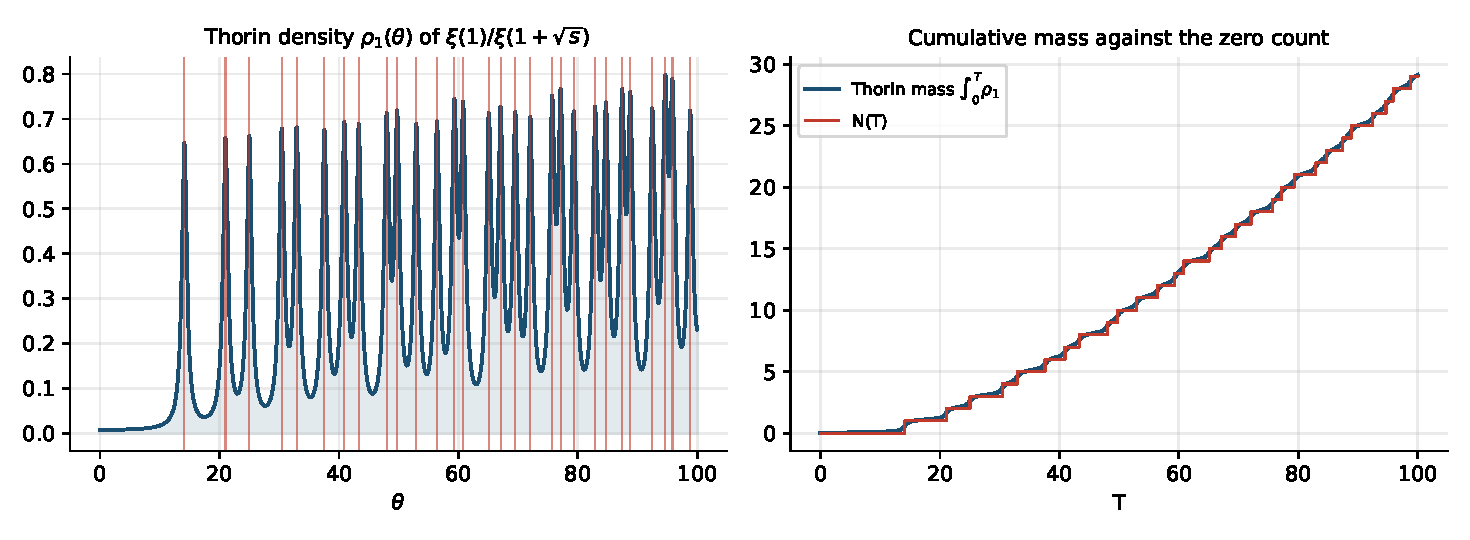
\includegraphics[width=\textwidth]{fig/bp1_density.pdf}
\caption{Left: the Thorin density $\rho_{1/2}(\theta)=v_1(\theta)/\pi$ of $T_1$ on $[0,100]$, with the ordinates of the zeros as thin vertical lines. Right: the cumulative Thorin mass $\int_0^T\rho_{1/2}$ against the zero count $N(T)$. The plot writes $\rho_1$ for $\rho_{1/2}$ and $s$ for $u$.}
\label{bp:fig:density}
\end{figure}

Because $\xi'(1)\ne0$, the Laplace transform of $T_1$ is not differentiable at the origin:
\[
\varphi_1(u)=1-\frac{\xi'}{\xi}(1)\sqrt u+O(u)=1-\Big(\sum_\rho\frac1\rho\Big)\sqrt u+O(u),\qquad u\downarrow0 .
\]
By the Tauberian theorem for Laplace transforms \cite[XIII.5]{Feller71}, $T_1$ has infinite mean and
\begin{equation}\label{bp:eq:tail}
P(T_1>x)\sim\frac{\sum_\rho\rho^{-1}}{\Gamma(\frac12)}\,x^{-1/2}=0.01303\,x^{-1/2},\qquad x\to\infty .
\end{equation}
Equivalently, near the origin the Thorin density in $z$ behaves like $\rho_{1/2}(0)/(2\sqrt z)$, which makes $\int U_1(dz)/z$ diverge. At the centre, by contrast, $\xi'(\frac12)=0$, the clock has the finite mean $\E T=\sum_ka_k^{-1}=0.0231050$, which is $\sum_{\gamma>0}\gamma^{-2}$ under RH, and the relevant constant is a sum over squared ordinates; at the basepoint one the constant is $\sum_\rho\rho^{-1}=0.0230957$, and it multiplies $\sqrt u$.

\subsection{The sine squared lemma at the basepoint one}\label{bp:sec:sin2}

At a basepoint $\alpha>1$ the sine squared lemma \eqref{eq:sin2}, applied to the canonical measure of $\log\xi$, writes $v_\alpha$ as the sum of a drift, an archimedean piece, a pole piece and a prime piece, \eqref{eq:split}. The pole piece is the image under the lemma of the measure $e^{-(\alpha-1)x}dx$ and it enters with a minus sign; the prime piece is positive. As $\alpha\downarrow1$ both diverge, the pole contribution to $-\infty$ and the prime piece to $+\infty$, because $\sum\Lambda(n)/n$ diverges (Section~\ref{sec:ch6:split}). So the lemma cannot be applied to the two pieces separately at the basepoint one. It can be applied to their difference. Throughout Section~\ref{ch:basepoint}, $\psi(y)=\sum_{n\le y}\Lambda(n)$ is Chebyshev's function, whose argument is always the real variable $y\ge1$ or the prime cutoff $X$, while at every other argument, as in $\psi(\frac32)$ or $\psi(\frac{1+i\theta}2)$, $\psi=\Gamma'/\Gamma$ is the digamma function; from here on $X$ always denotes the cutoff, not the P\'olya variable of Section~\ref{bp:sec:mellin}, and we write $\nu_1$ for the compensated prime measure of Proposition~\ref{bp:prop:sin2}, which is unrelated to the count $\nu(\sigma,T)$ of Section~\ref{ch:turing}.

\begin{proposition}\label{bp:prop:sin2}
Let $\nu_1=\sum_n\Lambda(n)n^{-1}\delta_{\log n}-\mathbf 1_{(0,\infty)}(x)\,dx$, the prime measure compensated by Lebesgue measure. For every $\theta\ne0$,
\begin{equation}\label{bp:eq:sin2one}
v_1(\theta)=\frac1{1+\theta^2}-\frac12\log\pi+\frac12\re\psi\Big(\frac{1+i\theta}2\Big)+\gamma_E+\lim_{X\to\infty}\int_0^{\log X}2\sin^2\Big(\frac{\theta x}2\Big)\nu_1(dx),
\end{equation}
that is, the limit of $\sum_{n\le X}\Lambda(n)n^{-1}2\sin^2(\frac12\theta\log n)-\big(\log X-\sin(\theta\log X)/\theta\big)$. The limit exists by the prime number theorem, and at $\theta=0$ the formula reduces to $v_1(0)=\sum_\rho\rho^{-1}$.
\end{proposition}

\begin{proof}
On the line $\re s=1$ the pole term $1/(s-1)=1/(i\theta)$ is purely imaginary, so $v_1(\theta)=\re\frac1{1+i\theta}-\frac12\log\pi+\frac12\re\psi(\frac{1+i\theta}2)+\re\frac{\zeta'}{\zeta}(1+i\theta)$. For $\re s\ge1$ with $s\ne1$, partial summation gives
\[
-\sum_{n\le X}\frac{\Lambda(n)}{n^s}+\int_1^Xy^{-s}dy=-\frac{\psi(X)-X}{X^s}-s\int_1^X(\psi(y)-y)\,y^{-s-1}dy-1,
\]
and the prime number theorem with the de la Vall\'ee Poussin error term, $\psi(y)-y=O(y\exp(-c\sqrt{\log y}))$, makes the boundary term vanish and the integral converge absolutely as $X\to\infty$, uniformly for $\re s\ge1$. For $\re s>1$ the limit is $\zeta'(s)/\zeta(s)+1/(s-1)$, and by continuity the same holds on $\re s=1$, $s\ne1$. Taking real parts at $s=1+i\theta$, where $\re\int_1^Xy^{-1-i\theta}dy=\sin(\theta\log X)/\theta$, gives $\re\frac{\zeta'}{\zeta}(1+i\theta)=\lim_X\big[-\sum_{n\le X}\Lambda(n)n^{-1}\cos(\theta\log n)+\sin(\theta\log X)/\theta\big]$. Writing $-\cos=2\sin^2-1$ and using $\sum_{n\le X}\Lambda(n)/n=\log X-\gamma_E+o(1)$, again a consequence of the prime number theorem, gives \eqref{bp:eq:sin2one}, since $\int_0^{\log X}2\sin^2(\theta x/2)dx=\log X-\sin(\theta\log X)/\theta$. At $\theta=0$ the bracket vanishes and $1-\frac12\log\pi+\frac12\psi(\frac12)+\gamma_E=1+\frac{\gamma_E}2-\frac12\log4\pi$.
\end{proof}

Table~\ref{bp:tab:sin2}, computed by \texttt{compute.py}, and Figure~\ref{bp:fig:sin2}, drawn by \texttt{figs.py}, check \eqref{bp:eq:sin2one} with primes up to $10^7$. The prime piece and the Lebesgue piece each grow like $\log X$, reaching about $16$ at $X=10^7$, and their difference converges to the exact value with an error that decreases roughly like $\log^2X/\sqrt X$, the rate the prime number theorem allows under RH.

\begin{table}[htbp]
\centering\small
\begin{tabular}{rrrrrr}
\toprule
$\theta$ & $X$ & prime piece & Lebesgue piece & formula \eqref{bp:eq:sin2one} & error\\
\midrule
5 & $10^3$ & 6.4288 & 6.9040 & 0.022767 & $-3.6\times10^{-3}$\\
5 & $10^5$ & 10.8715 & 11.3429 & 0.026558 & $1.5\times10^{-4}$\\
5 & $10^7$ & 15.8238 & 16.2955 & 0.026345 & $-6.1\times10^{-5}$\\
14.1347 & $10^3$ & 7.9028 & 6.9252 & 1.964685 & $-6.9\times10^{-2}$\\
14.1347 & $10^5$ & 12.5949 & 11.5547 & 2.027421 & $-6.4\times10^{-3}$\\
14.1347 & $10^7$ & 17.0932 & 16.0475 & 2.032931 & $-8.4\times10^{-4}$\\
30 & $10^3$ & 6.8808 & 6.9115 & 1.329190 & $5.0\times10^{-2}$\\
30 & $10^5$ & 11.4364 & 11.5191 & 1.277186 & $-1.7\times10^{-3}$\\
30 & $10^7$ & 16.0455 & 16.1267 & 1.278684 & $-2.4\times10^{-4}$\\
\bottomrule
\end{tabular}
\caption[The sine squared lemma at the basepoint one]{The sine squared lemma at the basepoint one: the prime piece $\sum_{n\le X}\Lambda(n)n^{-1}2\sin^2(\frac12\theta\log n)$, the Lebesgue piece $\log X-\sin(\theta\log X)/\theta$, the formula \eqref{bp:eq:sin2one} truncated at $X$, and its error against the exact values $v_1(\theta)=\pi\rho_{1/2}(\theta)=0.026406$, $2.033773$ and $1.278929$ at $\theta=5$, $14.1347$ and $30$.}
\label{bp:tab:sin2}
\end{table}

\begin{figure}[htbp]
\centering
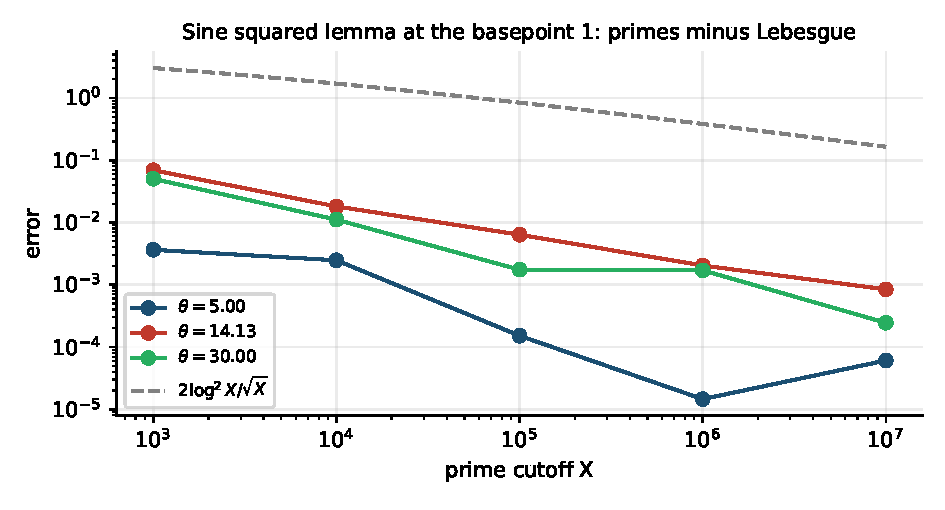
\includegraphics[width=0.72\textwidth]{fig/bp1_sin2.pdf}
\caption[Error of the compensated sine squared sum at the basepoint one]{Absolute error of the compensated sine squared sum \eqref{bp:eq:sin2one} against the prime cutoff $X$ at $\theta=5$, $14.13$ and $30$, with the reference rate $2\log^2X/\sqrt X$ (dashed).}
\label{bp:fig:sin2}
\end{figure}

So the Thorin density comes from the sine squared lemma, but its positivity does not. The lemma, applied to the compensated measure $\nu_1$, primes minus the uniform measure that represents the pole of $\zeta$, gives the arithmetic form of the density, and the existence of the sine squared integral of $\nu_1$ is the prime number theorem. Since $\nu_1$ is signed, its sine squared image is not termwise positive. Positivity comes from the zero side, Proposition~\ref{bp:prop:thorin}, through $\beta<1$, and written arithmetically it is the inequality
\[
-\re\frac{\zeta'}{\zeta}(1+it)<\frac1{1+t^2}-\frac12\log\pi+\frac12\re\psi\Big(\frac{1+it}2\Big),
\]
whose right side grows like $\frac12\log(t/2\pi)$: the inequality of Hadamard and de la Vall\'ee Poussin that underlies the proof of the prime number theorem \cite{Titchmarsh}. At the basepoint one the sine squared lemma and the prime number theorem are two readings of the same fact.

\subsection{The L\'evy form of \texorpdfstring{$\xi(1+s)$}{xi(1+s)}}\label{bp:sec:levy}

Section~\ref{bp:sec:sin2} started from the arithmetic formula for $v_1$. The sine squared lemma is designed to act one level earlier, on a L\'evy form of $\log\xi$ itself, which it converts into a Thorin form as described after \eqref{eq:sin2}, and at the basepoint one that L\'evy form exists and can be written down.

\begin{proposition}[L\'evy form]\label{bp:prop:levy}
For $\re s>0$,
\begin{equation}\label{bp:eq:levyform}
\log\frac{\xi(1+s)}{\xi(1)}=b_1s+\int_0^\infty\big(e^{-sx}-1+sx\big)\,\Pi_1(dx),
\end{equation}
with drift $b_1=-\frac12\log\pi+\frac12\psi(\frac32)+\gamma_E=\sum_\rho\rho^{-1}=0.0230957089661$ and the signed L\'evy measure
\[
\Pi_1(dx)=\Big(\frac{e^{-3x}}{1-e^{-2x}}-1\Big)\frac{dx}{x}+\sum_{n\ge2}\frac{\Lambda(n)}{n\log n}\,\delta_{\log n}(dx),
\]
the integral against the last two pieces being taken as $\lim_{X\to\infty}\int_0^{\log X}$.
\end{proposition}

\begin{proof}
Write $\xi(z)=(z-1)\pi^{-z/2}\Gamma(1+\frac z2)\zeta(z)$ and put $z=1+s$, so that $\xi(1+s)=\pi^{-(1+s)/2}\Gamma(\frac32+\frac s2)\,s\zeta(1+s)$ and $\xi(1)=\frac12$. Three classical formulas give the three pieces. The factor $\pi^{-s/2}$ contributes $-\frac s2\log\pi$. Binet's formula \cite[\S5.9]{DLMF}, $\log\Gamma(a+w)-\log\Gamma(a)=w\psi(a)+\int_0^\infty(e^{-wt}-1+wt)\frac{e^{-at}}{t(1-e^{-t})}dt$, with $a=\frac32$, $w=\frac s2$ and $t=2x$, contributes $\frac s2\psi(\frac32)$ and the density $e^{-3x}/(x(1-e^{-2x}))$. For the last factor, the Euler product gives $\log\zeta(1+s)=\sum_n\frac{\Lambda(n)}{n\log n}e^{-s\log n}$ for $\re s>0$, and Frullani's integral gives $\log s=\int_0^\infty(e^{-x}-e^{-sx})\frac{dx}x$. Their sum is $\log(s\zeta(1+s))$, which is analytic at $s=0$ with value $0$ and derivative $\gamma_E$, and subtracting the linear term puts it in the compensated form $\gamma_Es+\int(e^{-sx}-1+sx)\,x^{-1}\nu_1(dx)$, where $x^{-1}\nu_1(dx)=\sum\frac{\Lambda(n)}{n\log n}\delta_{\log n}-\frac{dx}x$. The compensated integral converges as $X\to\infty$ because the prime atoms and the measure $dx/x$ cancel at first order, by the prime number theorem in the form $\sum_{n\le X}\Lambda(n)/n=\log X-\gamma_E+o(1)$, and at zeroth order, by the logarithm of Mertens' product theorem \cite[Theorem 429]{boHardyWright}, $\sum_{p^k\le X}1/(kp^k)=\log\log X+\gamma_E+o(1)$, which does not need the prime number theorem (the logarithm of the product also contains the terms with $p\le X<p^k$, whose sum is $O(X^{-1/2})$). The drift is $\frac{d}{ds}\log\xi(1+s)|_{s=0}=\frac{\xi'}\xi(1)$.
\end{proof}

Table~\ref{bp:tab:levy}, computed by \texttt{levy.py}, checks \eqref{bp:eq:levyform} at $s=\frac12$, $1$ and $2$ with primes up to $10^7$. The prime piece and its compensator each grow like $s\log X$, reaching $28$ at $s=2$, and their difference approaches the exact value at the rate the prime number theorem allows.

\begin{table}[htbp]
\centering\small
\begin{tabular}{rrcccccc}
\toprule
$s$ & $X$ & $b_1s$ & gamma piece & primes & compensator & total & exact\\
\midrule
0.5 & $10^5$ & 0.01155 & 0.027227 & 3.40718 & 3.42845 & 0.017508 & 0.017311\\
0.5 & $10^7$ & 0.01155 & 0.027227 & 5.37344 & 5.39500 & 0.017217 & 0.017311\\
1 & $10^5$ & 0.02310 & 0.102283 & 8.41323 & 8.49224 & 0.046368 & 0.046118\\
1 & $10^7$ & 0.02310 & 0.102283 & 12.68129 & 12.76094 & 0.045729 & 0.046118\\
2 & $10^5$ & 0.04619 & 0.368975 & 19.03582 & 19.31202 & 0.138973 & 0.137917\\
2 & $10^7$ & 0.04619 & 0.368975 & 27.90836 & 28.18589 & 0.137639 & 0.137917\\
\bottomrule
\end{tabular}
\caption{The L\'evy form \eqref{bp:eq:levyform} against $\log(\xi(1+s)/\xi(1))$: the drift term, the gamma piece, the prime atoms up to $X$, their compensator, the total and the exact value.}
\label{bp:tab:levy}
\end{table}

The variable $V=V_1$ of Section~\ref{bp:sec:mellin}, the Esscher tilt by $e^{y/2}$ of the P\'olya density, has $\E e^{sV}=\xi(1+s)/\xi(1)$, so \eqref{bp:eq:levyform} has the form of a L\'evy Khintchine formula for the moment generating function of $V$, with $\Pi_1$, reflected to the negative half line by $x\mapsto-x$, in the place of the L\'evy measure. That measure is signed: the absolutely continuous part $\big(\frac{e^{-3x}}{1-e^{-2x}}-1\big)\frac1x$ is positive for $x<0.28120$, where the gamma factor dominates, and negative beyond, where the pole term $-dx/x$ dominates, and the only positive mass beyond is the prime atoms. So the uniqueness theorem for L\'evy triplets does not apply to $\Pi_1$ directly. Nor is $\Pi_1$ the signed L\'evy measure of a quasi infinitely divisible law in the sense of Lindner, Pan and Sato \cite{LPS18}, a law whose characteristic function is the quotient of two infinitely divisible ones: that would require the positive and negative parts of $\Pi_1$ to be L\'evy measures, of finite mass away from the origin, while on $(1,\infty)$ the positive part is the prime atoms and the negative part exceeds $0.94\,dx/x$, both of infinite mass, and they cancel only conditionally, which is why \eqref{bp:eq:levyform} holds only as a compensated limit. Proposition~\ref{sb:prop:qid}(3) proves that no other signed measure represents the characteristic function of $V$, so $V$ is not quasi infinitely divisible, and hence, since an infinitely divisible law is quasi infinitely divisible, not infinitely divisible. For every $\alpha>1$, by contrast, $V_\alpha$ is quasi infinitely divisible (Proposition~\ref{sb:prop:qid}(2)), so the basepoint one is exactly where the property is lost. The left panel of Figure~\ref{bp:fig:levy} shows the canonical measure $x\Pi_1(dx)$.

In the variable $\theta=\sqrt z$ the sine squared lemma \eqref{eq:sin2} reads
\[
e^{-sx}+sx-1=\frac{2x}\pi\int_0^\infty\log\Big(1+\frac{s^2}{\theta^2}\Big)\sin^2\Big(\frac{x\theta}2\Big)d\theta,\qquad\re s>0,\ x>0,
\]
and the drift converts through $\int_0^\infty\log(1+s^2/\theta^2)\,d\theta=\pi s$. Applying both to \eqref{bp:eq:levyform} and substituting $s=\sqrt u$ gives $\log\varphi_1(u)=-\int_0^\infty\log(1+u/\theta^2)\rho_{1/2}(\theta)\,d\theta$ with
\begin{equation}\label{bp:eq:conversion}
v_1(\theta)=b_1+\int_0^\infty2\sin^2\Big(\frac{x\theta}2\Big)\,x\Pi_1(dx)=b_1+A(\theta)+Q(\theta),
\end{equation}
where the drift $b_1$ is the stable part, $A(\theta)=\frac12\big[\re\psi(\frac{3+i\theta}2)-\psi(\frac32)\big]$ is the gamma piece and $Q(\theta)=\lim_{X\to\infty}\int_0^{\log X}2\sin^2(\frac{x\theta}2)\,\nu_1(dx)$ is the compensated prime piece. This is Proposition~\ref{bp:prop:sin2} again, now obtained by converting the L\'evy form rather than by manipulating $\re\xi'/\xi$; the two constant terms $-\frac12\log\pi+\gamma_E$ and $\frac12\psi(\frac32)$ combine into $b_1$, and $\frac12\re\psi(\frac{3+i\theta}2)=\frac12\re\psi(\frac{1+i\theta}2)+\frac1{1+\theta^2}$ accounts for the term $1/(1+\theta^2)$. With \texttt{levy.py} we checked that the sine squared integral of the gamma density equals the digamma expression $A(\theta)$ to ten digits at $\theta=5$, $14.1347$ and $30$ ($0.4749252962$, $0.9640604263$, $1.3367973267$).

The conversion has three readings, each visible in the right panel of Figure~\ref{bp:fig:levy}. First, the drift $b_1=\sum_\rho\rho^{-1}$ becomes the constant Thorin density $b_1/\pi$, which is the Thorin density of the positive stable one half factor $e^{-b_1\sqrt u}$. So $\varphi_1(u)=e^{-b_1\sqrt u}\exp\{-\int_0^\infty\log(1+u/\theta^2)(A+Q)(\theta)\,d\theta/\pi\}$, and the second factor is the transform of a GGC with Thorin density $(A+Q)/\pi$, because $v_1=b_1+A+Q$ attains its minimum $b_1$ only at the origin (Proposition~\ref{bp:prop:v1min}). The stable factor is the source of the tail $b_1(\pi x)^{-1/2}$ of \eqref{bp:eq:tail} and of the value $\rho_{1/2}(0)=b_1/\pi$, and it plays the role that the stable tilt plays for the floor of Section~\ref{rz:sec:floor}. At $u=(2k-1)^2$ the factorisation splits each coefficient $1/\zeta(2k)$ of Riesz's function \eqref{wr:eq:riesz}, up to an explicit factor, into a stable value and a GGC value (Section~\ref{ri:sec:ggc}). Second, the gamma factor contributes $A(\theta)\ge0$, smooth and growing like $\frac12\log(\theta/2)$: the average density of zeros. Third, the primes and the pole contribute $Q(\theta)$, which oscillates with both signs, between $-1.47$ and $1.04$ on $[0,100]$ (between $-1.29$ and $1.04$ on the window $[0,60]$ of the figure), and carries the peaks at the ordinates. Neither part converges alone; their compensated difference is the prime number theorem.

\begin{figure}[htbp]
\centering
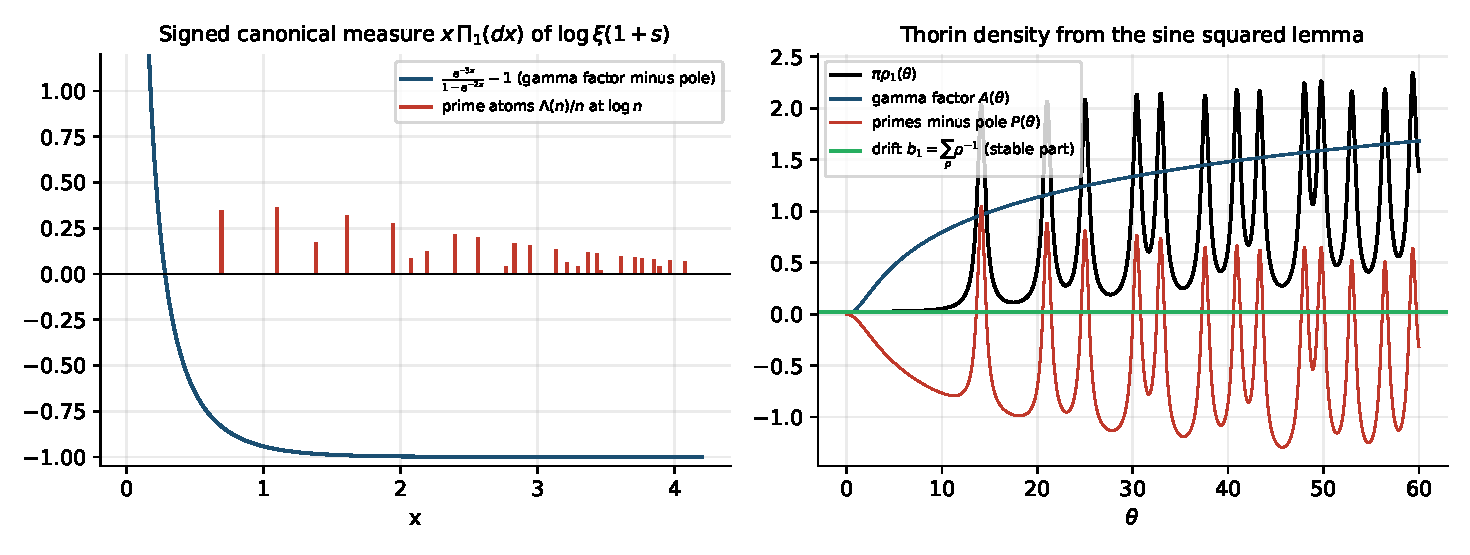
\includegraphics[width=\textwidth]{fig/bp1_levy.pdf}
\caption{Left: the signed canonical measure $x\Pi_1(dx)$ of $\log\xi(1+s)$, made of the gamma density minus the pole, $\big(\frac{e^{-3x}}{1-e^{-2x}}-1\big)dx$, which is negative beyond $x=0.28120$, and the prime atoms $\Lambda(n)/n$ at $\log n$ for $n\le60$. Right: the bracket $v_1(\theta)=\pi\rho_{1/2}(\theta)$ on $[0,60]$ assembled by the sine squared lemma from the drift $b_1$, the gamma piece $A(\theta)$ and the compensated prime piece $Q(\theta)$; the plot writes $\rho_1$ for $\rho_{1/2}$ and $P(\theta)$ for $Q(\theta)$. Drawn by \texttt{figs3.py}.}
\label{bp:fig:levy}
\end{figure}

The first reading needs $A+Q\ge0$, that is, $v_1\ge b_1$, at every height, and this holds with no hypothesis on the zeros. Near the origin $v_1$ is convex, at moderate heights a zero on the critical line is always close, and higher up every window of fixed length contains enough zeros for their Cauchy kernels to add up to more than $b_1$.

\begin{proposition}\label{bp:prop:v1min}
With no hypothesis on the zeros, $v_1(\theta)>v_1(0)=b_1$ for every real $\theta\ne0$; the proof uses a computation of the zeros below height $2000$ in ball arithmetic and, above that height, explicit bounds for the number of zeros up to a given height \cite{HSW22,Backlund}. Consequently $T_1\stackrel d=S+T_1^\circ$, where $S$ and $T_1^\circ$ are independent, $S$ is positive stable of index one half with $\E e^{-uS}=e^{-b_1\sqrt u}$, and $T_1^\circ$ is a GGC with no drift whose Thorin density in the chart $\theta=\sqrt z$ is $(v_1-b_1)/\pi=(A+Q)/\pi$.
\end{proposition}

\begin{proof}
By \eqref{bp:eq:rho1}, $v_1(\theta)=\pi\sum_\rho P_{1-\beta}(\theta-\gamma)$ is a sum of positive terms, with $\pi P_a(x)=a/(a^2+x^2)$, and $v_1$ is even, because $\xi$ is real on the real axis. We treat three ranges of $\theta\ge0$.

On $[0,13.5]$ we use convexity. Every zero has $|\gamma|\ge\gamma_1=14.134725$: the certified zeros of the next step, computed in order from the first, show that none has $0<|\gamma|<\gamma_1$, and none is real, because for $0<\sigma<1$ the alternating series $(1-2^{1-\sigma})\zeta(\sigma)=\sum_{n\ge1}(-1)^{n-1}n^{-\sigma}$ is positive while $1-2^{1-\sigma}<0$, so that $\zeta(\sigma)<0$. Since $\pi P_a''(x)=2a(3x^2-a^2)/(a^2+x^2)^3$, the kernel $P_a$ is strictly convex where $|x|>a/\sqrt3$, and for $|\theta|\le13.5$ every zero has $|\theta-\gamma|\ge\gamma_1-13.5>0.63>1/\sqrt3>(1-\beta)/\sqrt3$. So $v_1$ is strictly convex on $[-13.5,13.5]$, and, being even, it has there its unique minimum at $\theta=0$ and increases on $[0,13.5]$. By \eqref{eq:ch2:partial}, differentiated twice,
\[
v_1''(0)=-\Big(\frac{\xi'}\xi\Big)''(1)=\sum_\rho\frac{2(1-\beta)\big(3\gamma^2-(1-\beta)^2\big)}{\big((1-\beta)^2+\gamma^2\big)^3}>0 .
\]

On $[13.5,2000]$ we use the nearest zero. The script \texttt{v1min.py}, with output \texttt{v1min.json} (in the folders \texttt{riesz\_program/code} and \texttt{riesz\_program/data} of the archive), computes the first $1800$ zeros in ball arithmetic with Arb \cite{Arb}, which isolates them in order by Gram's law and Rosser's rule (Section~\ref{sec:ch5:turing}), each applied only in the range where it is known to hold \cite[Section 3]{Brent79}, so that none is missed. They reach height $2304.3$, all are simple and on the critical line, and consecutive ordinates differ by at most $\gamma_2-\gamma_1<6.8874$. Every $\theta\in[13.5,2000]$ therefore lies within $3.4437$ of an ordinate, half the largest gap, and a zero on the critical line at distance $x$ contributes $\pi P_{1/2}(x)=\frac12/(\frac14+x^2)$, which exceeds $b_1$ for $x<4.6259$. All other terms being positive,
\[
v_1(\theta)\ge\frac{1/2}{1/4+3.4437^2}>0.041,\qquad 13.5\le\theta\le2000 .
\]

For $\theta\ge2000$ we count zeros. Write $N(T)=\vartheta(T)/\pi+1+S(T)$ (Section~\ref{sec:ch5:turing}). Hasanalizade, Shen and Wong \cite[(1.7) and Corollary~1.4]{HSW22} give $|S(T)|\le2.5167$ for $0\le T\le X_0=30\,610\,046\,000$, from Platt's database of the zeros, and $|S(T)|\le0.1095\log T+0.2042\log\log T+3.0305$ for every $T\ge e$, and the smooth part $\vartheta(T)/\pi+1$ of $N(T)$ differs from $\frac T{2\pi}\log\frac T{2\pi e}+\frac78$ by at most $\frac1{50T}$ for $T\ge\frac57$ \cite[(2.7)]{HSW22}. So
\begin{multline*}
\Big|N(T)-\frac T{2\pi}\log\frac T{2\pi e}-\frac78\Big|\le E(T)\\
=\begin{cases}2.5167+\frac1{50T},&e\le T\le X_0,\\0.1095\log T+0.2042\log\log T+3.0305+\frac1{50T},&T>X_0,\end{cases}
\end{multline*}
and $E(T)<0.3\log T$ for $T>X_0$, since this holds at $X_0$ and $0.3-0.1095-0.2042/\log X_0>0$. The bound $0.112\log T+0.278\log\log T+2.510+0.2/T$ of Trudgian \cite{Trudgian}, which is often quoted, has an incomplete proof \cite{BMOR21,HSW22}. The error of Stirling's formula in the smooth part is $(\frac1{48T}+O(T^{-3}))/\pi$ \cite[Section 6.5]{Edwards}, and since the remainder of Stirling's series for $\log\Gamma(z)$ after the term $1/(12z)$ is at most $1/(90|z|^3)$ for $\re z>0$ \cite[\S5.11(ii)]{DLMF}, it is less than $0.01/T$ for $T\ge14$. The counts below use $\frac1{50T}$, as \texttt{v1min.py} does when it evaluates them; the sharper $0.01/T$, which the script also checks, would change them by less than $2\times10^{-5}$. Put $H=15$. The window $(\theta-H,\theta+H]$ holds $N(\theta+H)-N(\theta-H)$ zeros, counted with multiplicity, and since the main term has derivative $\frac1{2\pi}\log\frac T{2\pi}$, their number is at least
\[
n(\theta)=\frac H\pi\log\frac{\theta-H}{2\pi}-E(\theta-H)-E(\theta+H).
\]
While $\theta+H\le X_0$, $n$ increases, because $E$ decreases there, and $n(2000)>22.44$; for $\theta+H>X_0$, both values of $E$ are below $0.3\log(\theta+H)$, and $n(\theta)>\frac H\pi\log\frac{\theta-H}{2\pi}-0.6\log(\theta+H)>90$. So for every $\theta\ge2000$ the window holds at least $23$ zeros. Since $\xi(1-\bar s)=\overline{\xi(s)}$, the map $\rho\mapsto1-\bar\rho$ sends each zero to a zero of the same multiplicity; it keeps the ordinate and exchanges $\beta$ and $1-\beta$, so it permutes the zeros of the window, and the sum of $1-\beta$ over them is half their number. Each of them has $0<1-\beta<1$ and $|\theta-\gamma|\le H$, so its term $(1-\beta)/((1-\beta)^2+(\theta-\gamma)^2)$ in $v_1(\theta)$ exceeds $(1-\beta)/(1+H^2)$, and all other terms are positive. Hence
\[
v_1(\theta)>\frac{23}{2(1+H^2)}=\frac{23}{452}>0.05,\qquad \theta\ge2000,
\]
wherever the zeros lie. Backlund's classical constants $0.137$, $0.443$ and $4.35$, valid for $T\ge200$ \cite{Backlund}, give in the same way the increasing bound $E_B(T)=0.137\log T+0.443\log\log T+4.35+0.2/T$ in place of $E$ and at least $\frac H\pi\log\frac{\theta-H}{2\pi}-2E_B(\theta+H)$ zeros in the window, a number that increases with $\theta$ and exceeds $14.89$ at $\theta=2000$; the window then holds at least $15$ zeros, and the bound becomes $15/452>0.033$.

It remains to split $\varphi_1$. Since $\frac1\pi\int_0^\infty\log(1+u/\theta^2)\,d\theta=\sqrt u$, Proposition~\ref{bp:prop:thorin} gives
\[
\varphi_1(u)=e^{-b_1\sqrt u}\exp\Big\{-\frac1\pi\int_0^\infty\log\Big(1+\frac u{\theta^2}\Big)\big(v_1(\theta)-b_1\big)\,d\theta\Big\},\qquad u\ge0,
\]
where the integral is finite because $0\le v_1-b_1\le v_1$ and $\int_0^\infty\log(1+u/\theta^2)\,v_1(\theta)\,d\theta=-\pi\log\varphi_1(u)$ is finite by Theorem~\ref{thm:poisson} at $\alpha=1$. The first factor is the Laplace transform of the positive stable law of index one half with density $\frac{b_1}{2\sqrt\pi}t^{-3/2}e^{-b_1^2/(4t)}$. The image $U_1^\circ$ of $\pi^{-1}(v_1-b_1)\,d\theta$ under $\theta\mapsto\theta^2=z$ is a positive measure with $\int\log(1+u/z)\,U_1^\circ(dz)<\infty$, which is equivalent to the integrability condition in \eqref{eq:ch3:ggc}, so the second factor is the Laplace transform of a GGC $T_1^\circ$ with no drift. A product of Laplace transforms is the transform of the sum of independent variables, so $T_1\stackrel d=S+T_1^\circ$, and $v_1-b_1=A+Q$ by \eqref{bp:eq:conversion}.
\end{proof}

The factorisation separates the tail of $T_1$ from the rest of its law. The stable summand carries the infinite mean and the whole tail: $P(S>t)\sim b_1/\sqrt{\pi t}$ is the tail \eqref{bp:eq:tail} of $T_1$, while $T_1^\circ$ has finite mean and infinite variance. The Laplace exponent of $T_1^\circ$ is $\log(\xi(1+\sqrt u)/\xi(1))-b_1\sqrt u=\frac12(\log\xi)''(1)\,u+O(u^{3/2})$ as $u\downarrow0$, so that
\[
\E T_1^\circ=\frac12(\log\xi)''(1)=-\frac12\sum_\rho\rho^{-2}=0.0230772,
\]
and its Thorin density $(v_1-b_1)/\pi$ vanishes at the origin to exactly second order, since $v_1$ is even and $v_1''(0)>0$; for instance $v_1(1)-b_1=1.12\times10^{-4}$ and $v_1(5)-b_1=3.31\times10^{-3}$. Near $z=0$ the Thorin measure $U_1^\circ$ therefore has a density of exact order $\sqrt z$, and the variance $\int z^{-2}\,U_1^\circ(dz)$ is infinite. On $[13.5,2000]$ the smallest value of $v_1$ on the grid of step $0.02$ of \texttt{v1min.py} is $0.11326$, at $\theta=17.5$ in the valley between the first two ordinates, about five times $b_1$. An independent check, \texttt{v1\_grid\_mp.py} in the folder \texttt{repro}, evaluates the arithmetic form of $v_1$ with \texttt{mpmath} \cite{mpmath} to $25$ digits on the grid of step $0.005$ in $(0,2100]$. It finds $v_1>b_1$ at all $420000$ points, the smallest excess being $2.8\times10^{-9}$, at $\theta=0.005$, which is $0.005^2(v_1(1)-b_1)$ to two digits, as the vanishing to second order predicts; the smallest value on $[13.5,2000]$ is $0.1132554$, at $\theta=17.495$. The first $1850$ zeros, computed with \texttt{mpmath} by \texttt{zeros\_mp.py}, agree with those of Arb to double precision.

The same construction applies at every basepoint above one. For every $\alpha\ge1$ it gives the L\'evy form of $\log(\xi(\alpha+s)/\xi(\alpha))$ with drift $b_\alpha=\frac{\xi'}\xi(\alpha)$ and
\begin{gather*}
x\Pi_\alpha(dx)=\Big(\frac{e^{-(\alpha+2)x}}{1-e^{-2x}}-e^{-(\alpha-1)x}\Big)dx+\sum_n\frac{\Lambda(n)}{n^\alpha}\,\delta_{\log n}(dx),\\
v_\alpha(\theta)=b_\alpha+\int_0^\infty2\sin^2\Big(\frac{x\theta}2\Big)x\Pi_\alpha(dx),
\end{gather*}
which for $\alpha>1$ is \eqref{eq:split}. For $\alpha>1$ every piece converges on its own, and the pole contribution is the finite negative term $-\theta^2/((\alpha-1)((\alpha-1)^2+\theta^2))$. Expanding $1/(e^{2x}-1)=\sum_{k\ge1}e^{-2kx}$ in the archimedean piece of \eqref{eq:split}, and writing $q_c(\theta)=\int_0^\infty(1-\cos\theta x)e^{-cx}\,dx=\theta^2/(c(c^2+\theta^2))$, gives
\begin{equation}\label{bp:eq:excess}
v_\alpha(\theta)-b_\alpha=\sum_{k\ge1}q_{\alpha+2k}(\theta)-q_{\alpha-1}(\theta)+\sum_{n\ge2}\frac{\Lambda(n)}{n^\alpha}\big(1-\cos(\theta\log n)\big),\qquad\alpha>1 .
\end{equation}
Only the pole term is negative. Near the origin $q_c(\theta)\sim\theta^2/c^3$, and the pole term outweighs the gamma terms when $\alpha<7.789$, where $\frac18\zeta(3,\frac\alpha2+1)=(\alpha-1)^{-3}$; below that basepoint the arithmetic form needs the primes to keep $v_\alpha-b_\alpha$ positive near the origin. On the zero side positivity there is again convexity, and the factorisation of Proposition~\ref{bp:prop:v1min} holds at every basepoint above one.

\begin{proposition}\label{bp:prop:valpha}
With no hypothesis on the zeros, $v_\alpha(\theta)>v_\alpha(0)=b_\alpha$ for every $\alpha\ge1$ and every real $\theta\ne0$; the proof uses the zeros below height $2000$ of Proposition~\ref{bp:prop:v1min}, the explicit bounds of \cite{HSW22} for the number of zeros above that height, and a computation in ball arithmetic. Consequently, for every $\alpha\ge1$, $T_\alpha\stackrel d=S_\alpha+T_\alpha^\circ$, where $S_\alpha$ and $T_\alpha^\circ$ are independent, $S_\alpha$ is positive stable of index one half with $\E e^{-uS_\alpha}=e^{-b_\alpha\sqrt u}$, which is the law of the first passage time of Brownian motion to the level $b_\alpha/\sqrt2$, and $T_\alpha^\circ$ is a GGC with no drift, with Thorin density $(v_\alpha-b_\alpha)/\pi$ in the chart $\theta=\sqrt z$ and mean $\E T_\alpha^\circ=\frac12(\log\xi)''(\alpha)$.
\end{proposition}

\begin{proof}
At $\alpha=1$ this is Proposition~\ref{bp:prop:v1min}, so let $\alpha>1$. Since $v_\alpha$ is even, it suffices to take $\theta>0$. A zero $\rho=\beta+i\gamma$ contributes $a/(a^2+(\theta-\gamma)^2)$ to $v_\alpha(\theta)$, with $a=\alpha-\beta\in(\alpha-1,\alpha)$, and we put $\theta_0(\alpha)=\gamma_1-\alpha/\sqrt3$. Four steps cover all $\alpha>1$.

Near the origin, for $\alpha\le9$, we use convexity. If $0<\theta\le\theta_0(\alpha)$, every zero has $|\theta-\gamma|\ge\gamma_1-\theta\ge\alpha/\sqrt3>a/\sqrt3$, so, as in the proof of Proposition~\ref{bp:prop:v1min}, $v_\alpha$ is strictly convex on $[-\theta_0(\alpha),\theta_0(\alpha)]$, and $v_\alpha(\theta)>v_\alpha(0)$ there. Since $\theta_0(9)=8.94>0$, it remains to treat $\theta>\theta_0(\alpha)$ for $\alpha\le9$, and every $\theta>0$ for $\alpha>9$.

For $1<\alpha\le3$ we use the zeros. Here $\theta_0(\alpha)\ge\theta_0(3)=12.40$ and $\gamma_1-12.40<3.4437$, so by the computation in the proof of Proposition~\ref{bp:prop:v1min} every $\theta\in[\theta_0(\alpha),2000]$ lies within $3.4437$ of the ordinate of a zero on the critical line, whose term exceeds $r(\alpha)=(\alpha-\frac12)/((\alpha-\frac12)^2+3.4437^2)$. For $\theta\ge2000$ the window $(\theta-15,\theta+15]$ holds at least $20$ zeros, the sum of $a$ over them is $\alpha-\frac12$ times their number, and each term exceeds $a/(\alpha^2+225)$, so that $v_\alpha(\theta)>w(\alpha)=20(\alpha-\frac12)/(\alpha^2+225)$. The functions $r$ and $w$ increase on $[1,3]$, and so does $b_\alpha$, whose derivative $\sum_\rho(\gamma^2-a^2)/(a^2+\gamma^2)^2$ is positive for $\alpha<\gamma_1$. It therefore suffices that $r(\alpha_k)>b_{\alpha_{k+1}}$ and $w(\alpha_k)>b_{\alpha_{k+1}}$ at the points $\alpha_k=1+k/256$, and in ball arithmetic the smallest margins are $0.0180$ and $0.0209$.

For $3\le\alpha\le7$ we use the primes. Adding and subtracting $q_\alpha(\theta)$ in \eqref{bp:eq:excess}, dropping the prime terms and using $q_c(\theta)<1/c$ gives
\begin{align*}
v_\alpha(\theta)-b_\alpha>L(\alpha,\theta)&=\sum_{k\ge0}q_{\alpha+2k}(\theta)-\frac1\alpha-\frac1{\alpha-1}\\
&=\frac12\Big[\re\psi\Big(\frac{\alpha+i\theta}2\Big)-\psi\Big(\frac\alpha2\Big)\Big]-\frac1\alpha-\frac1{\alpha-1},
\end{align*}
which increases in $\theta$. Since $|\psi'(z)|\le\psi'(\re z)$ and $\psi'(x)\le1/x+1/x^2$ for $x>0$, $|\partial L/\partial\alpha|\le M(\alpha)=1/\alpha+3/\alpha^2+1/(\alpha-1)^2$, which decreases in $\alpha$. It therefore suffices that $L(\alpha_k,\theta_0(\alpha_{k+1}))>M(\alpha_k)/256$ at the points $\alpha_k=3+k/256$ of $[3,7]$; the smallest margin is $0.0228$, at $\alpha=7$, and the same check succeeds up to $\alpha=7.707$.

For $\alpha\ge7$ the gamma terms suffice. Since $q_c(\theta)$ decreases in $c$, $\sum_{k\ge1}q_{\alpha+2k}(\theta)\ge\frac12\int_{\alpha+2}^\infty q_c(\theta)\,dc=\frac14\log(1+\theta^2/(\alpha+2)^2)$, so with $A=\alpha+2$, $B=\alpha-1$ and $s=\theta^2$,
\[
v_\alpha(\theta)-b_\alpha\ge\Phi_\alpha(s)=\frac14\log\Big(1+\frac s{A^2}\Big)-\frac s{B(B^2+s)} .
\]
Here $\Phi_\alpha(0)=0$, and $\Phi_\alpha'(s)=1/(4(A^2+s))-B/(B^2+s)^2$ is nonnegative exactly when $(B^2+s)^2\ge4B(A^2+s)$, the two sides differing by a function that increases in $s$ when $B\ge2$. For $\alpha\ge9$ they are in this order already at $s=0$, because $B^3-4A^2=(\alpha-1)^3-4(\alpha+2)^2$ is $28$ at $\alpha=9$ and increases beyond, so $\Phi_\alpha(s)>0$ for every $s>0$, and no zero enters. For $7\le\alpha\le9$ and $\theta>\theta_0(\alpha)\ge\theta_0(9)$, we have $s>s_9=\theta_0(9)^2=79.90$, $6\le B\le8$ and $A\le11$, so $(B^2+s_9)^2\ge(36+s_9)^2>32(121+s_9)\ge4B(A^2+s_9)$; hence $\Phi_\alpha$ increases on $[s_9,\infty)$, where $\Phi_\alpha(s_9)\ge\frac14\log(1+s_9/121)-s_9/(6(36+s_9))>0.0118$.

The script \texttt{valpha\_min.py} in the folder \texttt{repro} carries out the checks of the last three steps in ball arithmetic with Arb \cite{Arb}, computing $b_\alpha$ from $\zeta(\alpha)$ and $\zeta'(\alpha)$. The factorisation follows from the inequality as in the proof of Proposition~\ref{bp:prop:v1min}, Theorem~\ref{thm:poisson} giving $\int_0^\infty\log(1+u/\theta^2)\,v_\alpha(\theta)\,d\theta<\infty$, and the mean is the coefficient of $u$ in $\log(\xi(\alpha+\sqrt u)/\xi(\alpha))-b_\alpha\sqrt u=\frac12(\log\xi)''(\alpha)\,u+O(u^{3/2})$.
\end{proof}

As at the basepoint one, $v_\alpha-b_\alpha$ starts as $c(\alpha)\theta^2$, with $c(\alpha)=-\frac12(\xi'/\xi)''(\alpha)>0$, so at every basepoint above one the Thorin density of $T_\alpha^\circ$ vanishes to second order at the origin, $T_\alpha^\circ$ has finite mean and infinite variance, and $S_\alpha$ carries the whole tail $P(T_\alpha>t)\sim b_\alpha/\sqrt{\pi t}$. The two summands move very differently with the basepoint. From $\alpha=1$ to $\alpha=9$ the drift $b_\alpha$ grows from $0.0230957$ to $0.3567685$, while the mean of the remainder falls only slowly, $\E T_\alpha^\circ$ being $0.0230772$, $0.0230425$, $0.0229942$, $0.0228577$, $0.0224351$, $0.0211082$ and $0.0176077$ at $\alpha=1$, $1.25$, $1.5$, $2$, $3$, $5$ and $9$; at the last six basepoints $c(\alpha)$ is $1.66$, $2.20$, $3.25$, $5.15$, $7.85$ and $8.85\times10^{-4}$ (computed by \texttt{valpha\_min.py}).

For $\alpha<1$ the Euler product no longer converges near $\re s=\alpha$, and the prime atoms $\Lambda(n)n^{-\alpha}$ can be compensated only if the primes are well enough distributed. So the route from the L\'evy form through the sine squared lemma computes the Thorin measure unconditionally on $\alpha\ge1$, the region where it is positive unconditionally; Section~\ref{bp:sec:below} shows exactly how far below the basepoint one it extends.

\subsection{Below the basepoint one}\label{bp:sec:below}

The construction of Section~\ref{bp:sec:levy} can be written down for any basepoint $\alpha=1-\varepsilon$ with $0<\varepsilon<\frac12$, and the question is whether it converges. Formally nothing changes except the pole term, which now grows: with $b_\alpha=\frac{\xi'}\xi(\alpha)$,
\[
x\Pi_\alpha(dx)=\frac{e^{-(\alpha+2)x}}{1-e^{-2x}}\,dx\;+\;\Big(\sum_n\frac{\Lambda(n)}{n^{\alpha}}\,\delta_{\log n}(dx)-e^{\varepsilon x}\,dx\Big),
\]
and the converted Thorin density would be $\pi^{-1}$ times
\begin{equation}\label{bp:eq:below}
b_\alpha+A_\alpha(\theta)+\lim_{X\to\infty}\Big[\sum_{n\le X}\frac{\Lambda(n)}{n^\alpha}\,2\sin^2\Big(\frac{\theta\log n}2\Big)-\int_0^{\log X}2\sin^2\Big(\frac{\theta x}2\Big)e^{\varepsilon x}dx\Big],
\end{equation}
with $A_\alpha(\theta)=\frac12\big[\re\psi(\frac{\alpha+2+i\theta}2)-\psi(\frac{\alpha+2}2)\big]$. The prime piece and the pole piece now each grow like $X^\varepsilon/\varepsilon$, and whether their difference converges is a question about how well $\psi(y)$ is approximated by $y$.

\begin{proposition}\label{bp:prop:below}
Let $\Theta=\sup\{\re\rho\}$ over the nontrivial zeros and let $\frac12<\alpha<1$.
\begin{enumerate}
\item If $\Theta<\alpha$, the L\'evy form $\log\frac{\xi(\alpha+s)}{\xi(\alpha)}=b_\alpha s+\int_0^\infty(e^{-sx}-1+sx)\Pi_\alpha(dx)$ holds for $\re s>0$, the compensated limit converging, and the sine squared lemma converts it into \eqref{bp:eq:below}, which then equals $v_\alpha(\theta)$ and is positive. The error of the compensated sum with prime cutoff $X$ is $O(X^{\Theta-\alpha+\delta})$ for every $\delta>0$.
\item Conversely, if the L\'evy form holds for $\re s>0$, then $\xi(\alpha+s)$ has no zeros with $\re s>0$, so $\Theta\le\alpha$.
\end{enumerate}
\end{proposition}

\begin{proof}
If $\Theta<\alpha$, the explicit formula gives $\psi(y)-y=O(y^{\Theta+\delta})$ for every $\delta>0$ \cite{Titchmarsh}. Then the Stieltjes integral $\int_1^\infty y^{-w}\,d(\psi(y)-y)$, which equals $-\frac{\zeta'}{\zeta}(w)-\frac1{w-1}$ for $\re w>1$, converges after one integration by parts for $\re w>\Theta$ and provides the analytic continuation there, with tail beyond $X$ of order $X^{\Theta-\re w+\delta}$. Taking $w=\alpha+s$ with $\re s\ge0$ and integrating twice in $s$ from $s=0$ gives the compensated L\'evy form, the gamma and polynomial factors being handled exactly as in Proposition~\ref{bp:prop:levy}. For fixed $\theta$ the sine squared lemma may be applied under the limit, because the compensated measure integrated against $2\sin^2(\theta x/2)$ is a combination of the same convergent Stieltjes integrals at $w=\alpha$ and $w=\alpha\pm i\theta$. Positivity follows from the Poisson form of Proposition~\ref{prop:struct}, as in Proposition~\ref{bp:prop:thorin}, with widths $\alpha-\beta>0$. Conversely, suppose the L\'evy form holds for $\re s>0$. Write $\nu_\alpha$ for the bracket in $x\Pi_\alpha$, so that the compensated part of the right side is the limit of $\int_0^{\log X}(e^{-sx}-1+sx)\,x^{-1}\nu_\alpha(dx)$; its part over $[0,1]$ is an entire function of $s$. For real $s>1-\alpha$ the integral $\int_1^\infty e^{-sx}x^{-1}\nu_\alpha(dx)$ converges absolutely, so the convergence of the compensated limit at two such values of $s$ gives that of $\int_1^{\log X}\nu_\alpha(dx)$ and of $\int_1^{\log X}x^{-1}\nu_\alpha(dx)$. The function $y\mapsto\int_1^y\nu_\alpha(dx)$ is therefore bounded on $[1,\infty)$, and one integration by parts against it shows that $\int_1^{\log X}e^{-sx}x^{-1}\nu_\alpha(dx)$ converges uniformly on compact subsets of $\re s>0$. So the compensated limit converges locally uniformly, the right side of the L\'evy form is analytic in $\re s>0$, hence so is $\log\xi(\alpha+s)$, and $\xi(\alpha+s)$ cannot vanish there.
\end{proof}

So the extension to $\xi(1-\varepsilon+s)$ exists exactly when $\zeta$ has no zeros in the half plane $\re s>1-\varepsilon$, up to the boundary case $\Theta=1-\varepsilon$. At the basepoint one the convergence of the compensated sum was the prime number theorem; at the basepoint $1-\varepsilon$ it is the estimate $\psi(y)-y=O(y^{1-\varepsilon+\delta})$, which is the zero free half plane $\re s>1-\varepsilon$; and as $\varepsilon\uparrow\frac12$ it is $\psi(y)-y=O(y^{1/2+\delta})$, which is RH. The L\'evy form route therefore reaches exactly as far as the zero free region does. It is an arithmetic restatement of step~7 of the path in Table~\ref{tab:ch25:path}, not a way around it.

Table~\ref{bp:tab:below}, computed by \texttt{below.py}, evaluates \eqref{bp:eq:below} with primes up to $10^7$ at $\theta=\gamma_1$ and compares it with $v_\alpha(\gamma_1)$ computed directly. On the range of the computation the primes behave as RH predicts, $\psi(y)-y=O(y^{1/2}\log^2y)$, so the errors should decay like $X^{1/2-\alpha}$, and they do (Figure~\ref{bp:fig:below}, left): the decay is fast at $\alpha=0.9$, slow at $\alpha=0.6$, where the prime and pole pieces are about $1500$ and their difference is still wrong by about $2$, and absent at the centre. At $\alpha=\frac12$ and $\theta=\gamma_1$ the compensated sum grows like $\log X$ (Figure~\ref{bp:fig:below}, right), which is the atom $\delta_{\gamma_1}$ of the RH measure forming as the cutoff increases; away from the zeros it oscillates without converging. The rate of convergence is thus itself a diagnostic: the exponent in $X^{\Theta-\alpha}$ measures the largest real part of a zero, although only up to the range of $X$ that can be computed, so it can never certify $\Theta$.

\begin{table}[htbp]
\centering\small
\begin{tabular}{cccccc}
\toprule
$\alpha$ & $X$ & prime piece & pole piece & formula \eqref{bp:eq:below} & $v_\alpha(\gamma_1)$\\
\midrule
1 & $10^7$ & 17.093 & 16.047 & 2.03293 & 2.03377\\
0.9 & $10^5$ & 23.250 & 21.754 & 2.50194 & 2.52704\\
0.9 & $10^7$ & 41.281 & 39.765 & 2.52202 & 2.52704\\
0.75 & $10^5$ & 70.611 & 67.856 & 3.79129 & 4.01691\\
0.75 & $10^7$ & 219.869 & 216.972 & 3.93394 & 4.01691\\
0.6 & $10^5$ & 257.280 & 251.510 & 6.84001 & 10.00677\\
0.6 & $10^7$ & 1537.254 & 1530.446 & 7.87829 & 10.00677\\
0.5 & $10^5$ & 653.402 & 642.998 & 11.497 & $+\infty$ (a zero)\\
0.5 & $10^7$ & 6114.332 & 6099.976 & 15.449 & $+\infty$ (a zero)\\
\bottomrule
\end{tabular}
\caption{The compensated sine squared formula \eqref{bp:eq:below} below the basepoint one at $\theta=\gamma_1$, with primes up to $X$, against the directly computed $v_\alpha(\gamma_1)=\re(\xi'/\xi)(\alpha+i\gamma_1)$; at $\alpha=\frac12$ the point $\frac12+i\gamma_1$ is a zero.}
\label{bp:tab:below}
\end{table}

\begin{figure}[htbp]
\centering
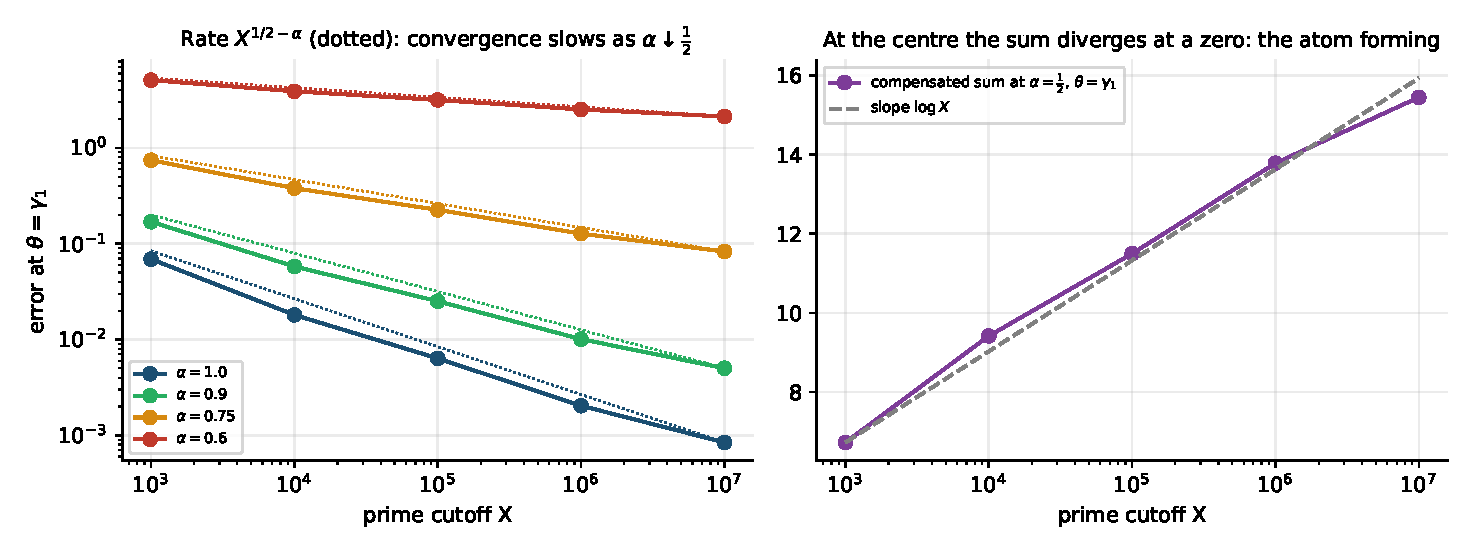
\includegraphics[width=\textwidth]{fig/bp1_below.pdf}
\caption{Left: absolute error of the compensated formula \eqref{bp:eq:below} at $\theta=\gamma_1$ against the prime cutoff $X$ for $\alpha=1$, $0.9$, $0.75$ and $0.6$, with the rates $X^{1/2-\alpha}$ (dotted). Right: at the centre, $\alpha=\frac12$, the compensated sum at the first ordinate grows like $\log X$ (dashed line), the atom of the RH measure forming. Drawn by \texttt{figs4.py}.}
\label{bp:fig:below}
\end{figure}

The slow convergence can be explained exactly, term by term over the zeros. Writing the tail of the compensated sum beyond $X$ as a Stieltjes integral against $d(\psi(y)-y)$ and inserting the explicit formula $\psi(y)=y-\sum_\rho y^\rho/\rho-\log2\pi-\frac12\log(1-y^{-2})$ \cite[Chapter~17]{Davenport} gives, for $\Theta<\alpha$ and $X$ not a prime power,
\begin{multline}\label{bp:eq:errformula}
\text{(formula \eqref{bp:eq:below} at cutoff }X)-v_\alpha(\theta)\\
=\sum_\rho\Big[-\frac{X^{\rho-\alpha}}{\rho-\alpha}+\frac{X^{\rho-\alpha+i\theta}}{2(\rho-\alpha+i\theta)}+\frac{X^{\rho-\alpha-i\theta}}{2(\rho-\alpha-i\theta)}\Big]+O(X^{-1-\alpha}),
\end{multline}
the sum taken over conjugate pairs. Every term has size $X^{\beta-\alpha}$, which makes the rate $X^{\Theta-\alpha}$ visible term by term, and at $\theta=\gamma$ the third term has denominator $\beta-\alpha$, so under RH it approaches $X^{1/2-\alpha}/(1-2\alpha)$ and at the centre it becomes the $\log X$ growth of Figure~\ref{bp:fig:below}. Table~\ref{bp:tab:err}, computed by \texttt{errformula.py}, compares the observed error with \eqref{bp:eq:errformula} truncated to the $1700$ zeros below height $2198$, and shows the error left after subtracting it. The explicit formula accounts for the error to four or five decimal places for $\alpha\ge0.75$ and to three at $\alpha=0.6$, and the hybrid of primes up to $X$ plus the first $1700$ zeros reduces the error of the primes alone by factors between about $700$ and $11000$: at $\alpha=0.6$ the error falls from $2.13$ to $7.7\times10^{-4}$.

\begin{table}[htbp]
\centering\small
\begin{tabular}{ccccc}
\toprule
$\alpha$ & $X$ & observed error & predicted by \eqref{bp:eq:errformula} & error after correction\\
\midrule
1 & $10^5$ & $-6.352\times10^{-3}$ & $-6.349\times10^{-3}$ & $-2.9\times10^{-6}$\\
1 & $10^7$ & $-8.419\times10^{-4}$ & $-8.431\times10^{-4}$ & $1.2\times10^{-6}$\\
0.9 & $10^7$ & $-5.014\times10^{-3}$ & $-5.020\times10^{-3}$ & $6.1\times10^{-6}$\\
0.75 & $10^7$ & $-8.297\times10^{-2}$ & $-8.304\times10^{-2}$ & $6.8\times10^{-5}$\\
0.6 & $10^5$ & $-3.1668$ & $-3.1665$ & $-2.9\times10^{-4}$\\
0.6 & $10^7$ & $-2.1285$ & $-2.1292$ & $7.7\times10^{-4}$\\
\bottomrule
\end{tabular}
\caption{The error of the compensated sum \eqref{bp:eq:below} at $\theta=\gamma_1$ with primes up to $X$, its prediction from the explicit formula \eqref{bp:eq:errformula} over the first $1700$ zeros, and what remains after subtracting the prediction.}
\label{bp:tab:err}
\end{table}

This also sharpens the logic of Proposition~\ref{bp:prop:below}. A zero with $\beta>\alpha$ would contribute a term of size $X^{\beta-\alpha}$ that grows with the cutoff, so the compensated sum at the basepoint $\alpha$ would diverge, and the size and phase of that growth would locate the zero. The hybrid formula is a zero detector with the same structure as Turing's method (Section~\ref{sec:ch5:turing}): primes up to $X$ and zeros up to height $T$ must balance to within the tail of both.

The role of the pole also changes below the basepoint one. If instead of compensating one continues the pole contribution analytically, its value at $\alpha=1-\varepsilon$ is $\re\frac1{-\varepsilon+i\theta}+\frac1\varepsilon=\frac{\theta^2}{\varepsilon(\varepsilon^2+\theta^2)}$, which is positive, since the pole now lies to the right of the basepoint. The single negative term of the decomposition \eqref{eq:split} above the basepoint one has become positive, and the difficulty has moved entirely into the prime sum, which no longer converges on its own. Below the line $\re s=1$, therefore, the negativity that RH must control is carried by the primes, not by the pole.

\subsection{The minimum at the origin below the basepoint one}\label{sec:dbeta:comp}

Propositions~\ref{bp:prop:v1min} and \ref{bp:prop:valpha} put the minimum of $v_\alpha$ at the origin for every $\alpha\ge1$, with no hypothesis on the zeros. Below the basepoint one the margin at the origin vanishes linearly, $b_\alpha\approx(\alpha-\frac12)(\log\xi)''(\frac12)$, and Table~\ref{bp:tab:alpha} found the minimum at the origin on a window by computation. This subsection proves it on the range of heights where the zeros are known to lie on the critical line, up to $\frac{1+\sqrt2}2$ below its top, for every basepoint $\alpha\in(\frac12,7.35]$, and shows that RH is equivalent to it at every height for every $\alpha\in(\frac12,1)$. The tool is a comparison across vertical lines, from the first author's note on the Dirichlet beta function \cite{P26beta}. It uses only the Hadamard product, the functional equation and an elementary bound on one line to the right of $\re s=1$, so it applies equally to the completed $L$ functions of Section~\ref{ch:chi12}. We state it for $f=\xi$, for $f=\xi(\cdot,\chi_4)$ of Section~\ref{sec:dbeta:beta} and for $f=\xi(\cdot,\chi_{12})$ of Section~\ref{sec:ch16:eta}, and write $v_\alpha(\theta)=\re(f'/f)(\alpha+i\theta)$, $b_\alpha=v_\alpha(0)=(f'/f)(\alpha)$ and $V_f=(\log f)''(\frac12)$. For the two $L$ functions the result is the full analogue of Proposition~\ref{bp:prop:valpha}.

Each $f$ is entire of order one, real on the real axis, with $f(s)=f(1-s)$ and no real zeros. Its zeros therefore come in groups: a zero $\frac12+i\gamma$ on the critical line, or a pair $\frac12\pm\delta+i\gamma$ with $0<\delta<\frac12$. At resolution $\varepsilon=\alpha-\frac12$ and offset $u=\theta-\gamma$, a zero on the line contributes $\varepsilon/(\varepsilon^2+u^2)$ to $v_\alpha(\theta)$, and a pair contributes
\begin{equation}\label{eq:dbeta:pair}
k_\delta(\varepsilon,u)=\frac{\varepsilon-\delta}{(\varepsilon-\delta)^2+u^2}+\frac{\varepsilon+\delta}{(\varepsilon+\delta)^2+u^2}=\frac{2\varepsilon(w+c)}{(w+c)^2+\kappa^2},
\end{equation}
where $w=\varepsilon^2$, $c=u^2-\delta^2$ and $\kappa=2\delta|u|$, since the numerator of the sum is $2\varepsilon(\varepsilon^2+u^2-\delta^2)$ and its denominator is $(\varepsilon^2+\delta^2+u^2)^2-4\varepsilon^2\delta^2=(w+c)^2+\kappa^2$. The pair contribution is negative exactly when $u^2<\delta^2-\varepsilon^2$, which is Proposition~\ref{prop:signature}(ii). The sum over the groups converges absolutely, since $\sum_\rho|\rho|^{-2}<\infty$. So $v_\alpha(\theta)/(\alpha-\frac12)$ is the sum over the groups of the ratios $1/(w+u^2)$ for the zeros on the line and
\[
r_\delta(w,u)=\frac{k_\delta(\varepsilon,u)}\varepsilon=2\re\frac1{w+c+i\kappa}
\]
for the pairs, as functions of $w=(\alpha-\frac12)^2$. The ratio of a zero on the line decreases in $w$; that of a pair need not.

\begin{lemma}[Comparison]\label{lem:dbeta:comp}
Let $0<\delta<\frac12$ and let $u$ be real. As a function of $w>0$, the ratio $r_\delta(w,u)$
\begin{enumerate}
\item[(a)] is nonincreasing on $(0,\infty)$ if $|u|\ge(1+\sqrt2)\delta$;
\item[(b)] is nonincreasing on $[2\delta^2,\infty)$ for every $u$, in particular on $w\ge\frac12$, that is for $\alpha\ge\frac12+\frac1{\sqrt2}$, whatever $\delta$;
\item[(c)] if $0<|u|<(1+\sqrt2)\delta$, increases exactly on the interval $\max\big(0,2\delta^2-(|u|+\delta)^2\big)<w<2\delta^2-(|u|-\delta)^2$, which begins at $0$ if and only if $|u|\ge(\sqrt2-1)\delta$; at $u=0$ it equals $2/(w-\delta^2)$, which has a pole at $w=\delta^2$.
\end{enumerate}
In particular the constant $1+\sqrt2$ in (a) cannot be lowered.
\end{lemma}

\begin{proof}
For $u\ne0$, $\partial_wr_\delta=-2\re(w+c+i\kappa)^{-2}=-2\big((w+c)^2-\kappa^2\big)/\big((w+c)^2+\kappa^2\big)^2$, which is positive exactly when $-\kappa<w+c<\kappa$, that is when $2\delta^2-(|u|+\delta)^2<w<2\delta^2-(|u|-\delta)^2$, since $-\kappa-c=2\delta^2-(|u|+\delta)^2$ and $\kappa-c=2\delta^2-(|u|-\delta)^2$. The right end is at most $2\delta^2$, which gives (b) for $u\ne0$; it is positive exactly when $\big||u|-\delta\big|<\sqrt2\delta$, that is when $|u|<(1+\sqrt2)\delta$, which gives (a) and the first part of (c); and the left end is at most $0$ exactly when $|u|+\delta\ge\sqrt2\delta$. At $u=0$, $c=-\delta^2$ and $\kappa=0$, and $2/(w-\delta^2)$ decreases on $w>\delta^2$, which completes (b). Finally $2\delta^2<\frac12$ because $\delta<\frac12$.
\end{proof}

So for $(\sqrt2-1)\delta\le|u|<(1+\sqrt2)\delta$ the ratio of a pair increases from $w=0$ up to $w=2\delta^2-(|u|-\delta)^2$, while for $0<|u|<(\sqrt2-1)\delta$ it first decreases and then increases up to that point; in both cases it decreases beyond it. Summing the lemma over the groups gives the comparison.

\begin{theorem}[Comparison across vertical lines]\label{thm:dbeta:comp}
Let $\frac12<\alpha<\alpha'$ and let $\theta$ be real. Suppose that every zero $\frac12+\delta+i\gamma$ of $f$ with $\delta>(\alpha-\frac12)/\sqrt2$ satisfies $|\theta-\gamma|\ge(1+\sqrt2)\delta$. Then
\[
\frac{v_\alpha(\theta)}{\alpha-\frac12}\ \ge\ \frac{v_{\alpha'}(\theta)}{\alpha'-\frac12}.
\]
The hypothesis holds at every $\theta$ under RH for $\xi$, or GRH for $\chi_4$ or $\chi_{12}$; at every $\theta$ when $\alpha\ge\frac12+\frac1{\sqrt2}$, with no hypothesis; and at every $\theta$ with $|\theta|\le H_0-\frac{1+\sqrt2}2$, where $H_0$ is a height below which every zero of $f$ is known to lie on the critical line: $H_0=3\times10^{12}$ for $\xi$ \cite{PT21}, and $H_0=10^8/q$ for $\xi(\cdot,\chi_q)$, that is $2.5\times10^7$ for $\chi_4$ and $10^8/12>8.33\times10^6$ for $\chi_{12}$ \cite{Platt16}.
\end{theorem}

\begin{proof}
A zero on the line has the ratio $1/(w+u^2)$, which decreases in $w$. A pair with $\delta\le(\alpha-\frac12)/\sqrt2$ has $2\delta^2\le(\alpha-\frac12)^2$, so its ratio is nonincreasing on $[(\alpha-\frac12)^2,(\alpha'-\frac12)^2]$ by Lemma~\ref{lem:dbeta:comp}(b), and a pair with $|\theta-\gamma|\ge(1+\sqrt2)\delta$ by Lemma~\ref{lem:dbeta:comp}(a). Summing over the groups, which converges absolutely, gives the inequality. Under RH there are no pairs. If $\alpha\ge\frac12+\frac1{\sqrt2}$, every pair has $\delta<\frac12\le(\alpha-\frac12)/\sqrt2$. If $|\theta|\le H_0-\frac{1+\sqrt2}2$, every zero off the line has $|\gamma|>H_0$, so that $|\theta-\gamma|>\frac{1+\sqrt2}2>(1+\sqrt2)\delta$.
\end{proof}

Table~\ref{tab:dbeta:ratio} shows the ratio along rows of basepoints at three heights for each function. Every row decreases, and at $\theta=0$ the rows approach $V_f$ from below, as part (i) of Theorem~\ref{thm:dbeta:minall} below states.

\begin{table}[htbp]
\centering\footnotesize
\fitwidth{\begin{tabular}{llccccccc}
\toprule
$f$ & $\theta$ & $\alpha=0.55$ & $0.6$ & $0.75$ & $1$ & $1.5$ & $2.5$ & $\alpha'$\\
\midrule
$\xi$ & $0$ & $0.0462098$ & $0.0462092$ & $0.0462053$ & $0.0461914$ & $0.0461359$ & $0.0459171$ & $0.0449540$\\
 & $20$ & $1.07455$ & $1.06774$ & $1.02263$ & $0.891327$ & $0.606114$ & $0.308661$ & $0.142788$\\
 & $40$ & $1.55119$ & $1.54053$ & $1.47072$ & $1.27476$ & $0.878717$ & $0.478933$ & $0.223196$\\
$\xi(\cdot,\chi_4)$ & $0$ & $0.156025$ & $0.156011$ & $0.155914$ & $0.155568$ & $0.154215$ & $0.149240$ & $0.144828$\\
 & $10$ & $16.4457$ & $14.7010$ & $8.49762$ & $3.52441$ & $1.22477$ & $0.492101$ & $0.363147$\\
 & $40$ & $10.4644$ & $9.84566$ & $7.06888$ & $3.83983$ & $1.77007$ & $0.837764$ & $0.622760$\\
$\xi(\cdot,\chi_{12})$ & $0$ & $0.332896$ & $0.332812$ & $0.332226$ & $0.330167$ & $0.322371$ & & $0.302579$\\
 & $10$ & $1.93963$ & $1.93082$ & $1.87180$ & $1.69298$ & $1.26262$ & & $0.800089$\\
 & $40$ & $6.07381$ & $5.93675$ & $5.16314$ & $3.71050$ & $2.10812$ & & $1.19861$\\
\bottomrule
\end{tabular}}
\caption{The ratio $v_\alpha(\theta)/(\alpha-\frac12)$ of Theorem~\ref{thm:dbeta:comp} along rows of basepoints. The last column is at the comparison line $\alpha'$ of Table~\ref{tab:dbeta:minall} taken from the first author's note: $4.75$ for $\xi$, $3.15$ for $\chi_4$ and $2.30$ for $\chi_{12}$, which lies below $2.5$. Every row decreases, and at $\theta=0$ the rows increase to $V_f$ as $\alpha\downarrow\frac12$ (Table~\ref{tab:dbeta:minall}). Computed by \texttt{dbeta\_minimum.py}.}
\label{tab:dbeta:ratio}
\end{table}

On a line to the right of $\re s=1$ the Euler product bounds $v_\alpha$ from below, and the comparison carries the bound to the left.

\begin{corollary}[Explicit lower bound]\label{cor:dbeta:lower}
For $\sigma>1$ and real $\theta$, $v_\sigma(\theta)\ge A^\infty_f(\sigma,\theta)-S_f(\sigma)$, where
\begin{gather*}
A^\infty_\xi(\sigma,\theta)=-\tfrac12\log\pi+\tfrac12\re\psi\big(\tfrac{\sigma+i\theta}2\big),\\
A^\infty_{\chi_4}(\sigma,\theta)=\tfrac12\log\tfrac4\pi+\tfrac12\re\psi\big(\tfrac{\sigma+1+i\theta}2\big),\\
A^\infty_{\chi_{12}}(\sigma,\theta)=\tfrac12\log\tfrac{12}\pi+\tfrac12\re\psi\big(\tfrac{\sigma+i\theta}2\big),\\
S_f(\sigma)=\sum_{(n,q)=1}\frac{\Lambda(n)}{n^\sigma},
\end{gather*}
with $q=1$, $4$ and $12$ for the three functions, so that $S_\xi=-\zeta'/\zeta$, $S_{\chi_4}(\sigma)=S_\xi(\sigma)-\log2/(2^\sigma-1)$ and $S_{\chi_{12}}(\sigma)=S_{\chi_4}(\sigma)-\log3/(3^\sigma-1)$; and $A^\infty_f(\sigma,\theta)$ increases in $|\theta|$. Hence, under the hypothesis of Theorem~\ref{thm:dbeta:comp} with $\alpha'>1$,
\begin{align*}
v_\alpha(\theta)&\ \ge\ \frac{\alpha-\frac12}{\alpha'-\frac12}\Big(A^\infty_f(\alpha',\theta)-S_f(\alpha')\Big)\\
&\ =\ \frac{\alpha-\frac12}{2\alpha'-1}\log|\theta|+O(1),\qquad|\theta|\to\infty .
\end{align*}
\end{corollary}

\begin{proof}
For $\re s>1$,
\[
\frac{\xi'}\xi(s)=\frac1s+\frac1{s-1}-\frac12\log\pi+\frac12\psi\Big(\frac s2\Big)+\frac{\zeta'}\zeta(s),
\]
where $\re(\frac1s+\frac1{s-1})\ge0$ and $\re\frac{\zeta'}\zeta(\sigma+i\theta)=-\sum_n\Lambda(n)n^{-\sigma}\cos(\theta\log n)\ge-S_\xi(\sigma)$; for the two $L$ functions the bound is that of Proposition~\ref{prop:dbeta:termwise}. The monotonicity in $|\theta|$ follows from the series $\re\psi(x+iy)-\psi(x)=\sum_{k\ge0}y^2/\big((x+k)((x+k)^2+y^2)\big)$, and $\re\psi(x+iy)=\log|y|+O(1)$ for fixed $x>0$. Then apply Theorem~\ref{thm:dbeta:comp} between $\alpha$ and $\alpha'$.
\end{proof}

\begin{remark}[A bound of order $\log\theta$ outside a sparse set]\label{rem:dbeta:average}
For fixed $\alpha>\frac12$ the hypothesis of Theorem~\ref{thm:dbeta:comp} fails only at heights within $(1+\sqrt2)\delta<\frac{1+\sqrt2}2$ of the ordinate of a zero $\frac12+\delta+i\gamma$ with $\delta>(\alpha-\frac12)/\sqrt2$. For $f=\xi$ the number of such zeros with $0<\gamma\le T$ is $N(\sigma_0,T)$ with $\sigma_0=\frac12+(\alpha-\frac12)/\sqrt2>\frac12$, which is $O(T^{3(1-\sigma_0)/(2-\sigma_0)}\log^5T)=o(T)$ by Ingham's estimate \cite{Ingham40} (Section~\ref{ag:sec:almost}). So Corollary~\ref{cor:dbeta:lower} with $\alpha'=\alpha+1$ gives $v_\alpha(\theta)/\pi\ge c\log\theta$, for every $c<(\alpha-\frac12)/(\pi(2\alpha+1))$ and all large $\theta$, outside a set of heights of density zero: this is the lower bound of the first of the four questions of Section~\ref{ag:sec:exactly}, for the density $v_\alpha/\pi$ itself. The exceptional set, however, contains the window of every zero to the right of the line $\re s=\alpha$, since such a zero has $\delta>\alpha-\frac12>(\alpha-\frac12)/\sqrt2$. So the bound gives no information where Lemma~\ref{ag:lem:cancel} would need it, and it does not by itself confine a failure of positivity to the thin strips of that question.
\end{remark}

\begin{theorem}[Minimum at the origin]\label{thm:dbeta:minall}
Let $V_f$, $\gamma_1$, $H_0$ and $\alpha_{\max}$ be as in Table~\ref{tab:dbeta:minall}.
\begin{enumerate}
\item[(i)] For every $\alpha>\frac12$, $0<b_\alpha\le(\alpha-\frac12)V_f$; the ratio $b_\alpha/(\alpha-\frac12)$ decreases in $\alpha$ and tends to $V_f$ as $\alpha\downarrow\frac12$.
\item[(ii)] For $\frac12<\alpha\le\alpha_{\max}$, $v_\alpha(\theta)>b_\alpha$ for $0<|\theta|\le H_0-\frac{1+\sqrt2}2$.
\item[(iii)] For $\frac12+\frac1{\sqrt2}\le\alpha\le\alpha_{\max}$, $v_\alpha(\theta)>b_\alpha$ for every $\theta\ne0$.
\item[(iv)] For $f=\xi(\cdot,\chi_4)$ and $f=\xi(\cdot,\chi_{12})$, $v_\alpha(\theta)>b_\alpha$ for every $\alpha\ge\frac12+\frac1{\sqrt2}$ and every $\theta\ne0$.
\item[(v)] For $f=\xi(\cdot,\chi_4)$ and $f=\xi(\cdot,\chi_{12})$, $v_\alpha(\theta)>b_\alpha$ for every $\alpha\ge1$ and every $\theta\ne0$.
\item[(vi)] RH, respectively GRH for $\chi_4$ or for $\chi_{12}$, holds if and only if $v_\alpha(\theta)>b_\alpha$ for every $\alpha\in(\frac12,1)$ and every $\theta\ne0$.
\end{enumerate}
\end{theorem}

\begin{proof}
(i) The function $f(\frac12+s)=\int_{\R}K(u)e^{su}\,du$ is the two sided Laplace transform of a positive even kernel $K$: the P\'olya kernel $\Phi$ for $\xi$ (Section~\ref{ch:clock}), the kernel $K_4$ of Proposition~\ref{prop:dbeta:kernel}, and the eta kernel of Section~\ref{sec:ch16:eta}. So $\log f(\frac12+s)$ is, up to a constant, the cumulant generating function of a nondegenerate law; it is even and strictly convex in real $s$, and $b_\alpha=(\log f)'(\alpha)=\int_{1/2}^\alpha(\log f)''(r)\,dr>0$. At $\theta=0$ the offset of a group with ordinate $\gamma$ has $|u|=|\gamma|\ge\gamma_1>\frac{1+\sqrt2}2>(1+\sqrt2)\delta$, so by Lemma~\ref{lem:dbeta:comp}(a) the ratio of every group is nonincreasing in $w$, strictly for the zeros on the line, and $b_\alpha/(\alpha-\frac12)$, their sum, decreases in $\alpha$. As $w\downarrow0$ the ratios increase to $\gamma^{-2}$ for a zero on the line and to $2\re(|\gamma|+i\delta)^{-2}$ for a pair, and by monotone convergence the sum tends to the sum of these limits, which is $-\sum_\rho(\frac12-\rho)^{-2}=(\log f)''(\frac12)=V_f$.

(ii) Put $\alpha'=\alpha_{\max}$ and let $t_1$ be its value at $\alpha_{\max}$ in Table~\ref{tab:dbeta:minall}, where $A^\infty_f(\alpha',t_1)-S_f(\alpha')>(\alpha'-\frac12)V_f$ is certified in ball arithmetic; since $A^\infty_f$ increases in $|\theta|$, the inequality holds for $|\theta|\ge t_1$. For $t_1\le|\theta|\le H_0-\frac{1+\sqrt2}2$, Corollary~\ref{cor:dbeta:lower} and (i) give $v_\alpha(\theta)>(\alpha-\frac12)V_f\ge b_\alpha$ (for $\alpha=\alpha'$ the comparison is an identity). For $|\theta|\le t_1$ we show that $v_\alpha$ is strictly convex on $[-t_1,t_1]$; as it is even, it then exceeds $v_\alpha(0)=b_\alpha$ at $0<|\theta|\le t_1$. The term $\varphi(\theta-\gamma)$, $\varphi(x)=a/(a^2+x^2)$ with $a=\alpha-\frac12$, of a zero on the line is strictly convex where $|\theta-\gamma|>a/\sqrt3$, since $\varphi''(x)=2a(3x^2-a^2)/(a^2+x^2)^3$. Below $H_0$ all zeros lie on the line and have $|\gamma|\ge\gamma_1$, and for $|\theta|\le t_1$, $|\theta-\gamma|\ge\gamma_1-t_1>(\alpha'-\frac12)/\sqrt3\ge a/\sqrt3$ by the convexity margin of the table. Every zero above $H_0$ has $|\theta-\gamma|>H_0-t_1>10^6$. For a pair there, the second derivative in $\theta$ of $k_\delta(a,\theta-\gamma)$ is $g(a+\delta,u)+g(a-\delta,u)$ with $g(c,u)=2c(3u^2-c^2)/(c^2+u^2)^3$, the second derivative of $c/(c^2+u^2)$ in $u$; since $\partial_cg(c,u)=6(u^4-6c^2u^2+c^4)/(c^2+u^2)^4>0$ for $|c|<(\sqrt2-1)|u|$, and $|a\pm\delta|<\alpha_{\max}<(\sqrt2-1)10^6$, the odd function $g(\cdot,u)$ increases on an interval containing $\pm(a\pm\delta)$, so that $g(a+\delta,u)>g(\delta-a,u)=-g(a-\delta,u)$. The sum of the second derivatives converges uniformly on $[-t_1,t_1]$, so $v_\alpha''>0$ there.

(iii) For $\alpha\ge\frac12+\frac1{\sqrt2}$ the hypothesis of Theorem~\ref{thm:dbeta:comp} holds at every $\theta$, so the bound of (ii) holds for every $|\theta|\ge t_1$, and the convexity argument for $|\theta|\le t_1$ is unchanged.

(iv) It remains to treat $\alpha>\alpha_{\max}$, and there we use the primes. For $\chi_4$, $v_\alpha(\theta)-b_\alpha=G_\alpha(\theta)+\varpi_\alpha(\theta)$ by \eqref{eq:dbeta:sin2}, with $G_\alpha(\theta)=\frac12[\re\psi(\frac{\alpha+1+i\theta}2)-\psi(\frac{\alpha+1}2)]$; for $\chi_{12}$ the same holds with $G_\alpha(\theta)=\frac12[\re\psi(\frac{\alpha+i\theta}2)-\psi(\frac\alpha2)]$ and the weights $\chi_{12}(n)\Lambda(n)$ (Section~\ref{sec:ch16:sin2}). Dropping the positive weights and bounding $1-\cos x$ by $2$ and by $x^2/2$ gives $\varpi_\alpha(\theta)\ge-R_\alpha(\theta)$ with $R_\alpha(\theta)\le\min\big(2S^-(\alpha),\frac12\theta^2M_2(\alpha)\big)$, where
\begin{align*}
S^-(\alpha)&=\sum_{\chi(n)=-1}\frac{\Lambda(n)}{n^\alpha}=\frac12\Big(S_f(\alpha)+\frac{L'}L(\alpha)\Big),\\
M_2(\alpha)&=\sum_{\chi(n)=-1}\frac{\Lambda(n)\log^2n}{n^\alpha}=\frac12\Big(S_f''(\alpha)+\Big(\frac{L'}L\Big)''(\alpha)\Big).
\end{align*}
The function $G_\alpha(\theta)$ is a sum of terms $q_c(\theta)=\theta^2/(c(c^2+\theta^2))$, so it increases in $|\theta|$ and decreases in $\alpha$, and $G_\alpha(\theta)/\theta^2$ decreases in $|\theta|$; and $S^-$ and $M_2$ decrease in $\alpha$. So on a cell $s_0\le\alpha\le s_1$ it suffices that $G_{s_1}(T)>\max\big(2S^-(s_0),\frac12T^2M_2(s_0)\big)$ for one $T>0$: then $G_\alpha(\theta)\ge G_{s_1}(T)>2S^-(\alpha)$ for $|\theta|\ge T$, and $G_\alpha(\theta)\ge\theta^2G_{s_1}(T)/T^2>\frac12\theta^2M_2(\alpha)$ for $0<|\theta|\le T$. The script \texttt{dbeta\_minimum.py} checks this in ball arithmetic on cells of width $\frac1{32}$ covering $[\sigma_2,20]$, with $T\in\{0.25,0.5,\dots,4\}$, where $\sigma_2=3.71875$ for $\chi_4$ and $2.8125$ for $\chi_{12}$; the cells just below $\sigma_2$ fail. For $\alpha\ge20$ take $T=2$: since $q_c$ decreases in $c$, $G_\alpha(2)\ge\frac12\int_{\alpha+1}^\infty q_c(2)\,dc=\frac14\log(1+4/(\alpha+1)^2)\ge1/((\alpha+1)^2+4)$, and since every $n$ with $\chi(n)=-1$ is at least $3$, $S^-(\alpha)$ and $M_2(\alpha)$ are at most $3^{-(\alpha-20)}$ times their values at $20$. With $K=\max(2S^-(20),2M_2(20))$ it therefore suffices that $K((\alpha+1)^2+4)3^{-(\alpha-20)}<1$ for $\alpha\ge20$; the left side decreases in $\alpha$, and at $\alpha=20$ it is $3.4\times10^{-7}$ for $\chi_4$ and $3.9\times10^{-11}$ for $\chi_{12}$. As $\alpha_{\max}=4.70>3.71875$ for $\chi_4$ and $3.10>2.8125$ for $\chi_{12}$, (iii) and this argument cover every $\alpha\ge\frac12+\frac1{\sqrt2}$.

(v) By (ii) and (iv) it remains to treat $1\le\alpha<\frac12+\frac1{\sqrt2}$ and $|\theta|>H_0-\frac{1+\sqrt2}2$, and by symmetry $\theta>0$. Let $n$ be the number of zeros with $|\gamma-\theta|\le h$, counted with multiplicity, where $h=15$ for $\chi_4$ and $h=10$ for $\chi_{12}$. Every zero has $0<\beta<1\le\alpha$, so every term of $v_\alpha(\theta)$ is positive, and a zero in the window contributes $a/(a^2+(\theta-\gamma)^2)\ge a/(\alpha^2+h^2)$, with $a=\alpha-\beta\in(0,\alpha)$; the window contains both members of each pair $\frac12\pm\delta+i\gamma$, whose values of $a$ add up to $2(\alpha-\frac12)$, so the values of $a$ over the window add up to $n(\alpha-\frac12)$. Hence $v_\alpha(\theta)>n(\alpha-\frac12)/(\alpha^2+h^2)$, which is at least $(\alpha-\frac12)V_f\ge b_\alpha$ as soon as $n\ge V_f(\alpha^2+h^2)$. Since $\alpha^2<(\frac12+\frac1{\sqrt2})^2=1.4571\ldots$, it suffices that $n>35.335$ for $\chi_4$ and $n>33.778$ for $\chi_{12}$. By the explicit counting formula of Bennett, Martin, O'Bryant and Rechnitzer \cite[Theorem 1.1]{BMOR21}, for a primitive character $\chi$ of conductor $q>1$, $T\ge\frac57$ and $\ell=\log(q(T+2)/(2\pi))>1.567$, the number $N(T,\chi)$ of zeros with $|\gamma|\le T$ satisfies
\[
\Big|N(T,\chi)-\frac T\pi\log\frac{qT}{2\pi e}+\frac{\chi(-1)}4\Big|\le E(T)=0.22737\,\ell+2\log(1+\ell)-0.5 .
\]
As $f$ has no real zeros and its zeros are symmetric about the real axis, $N(\theta+h,\chi)-N(\theta-h,\chi)$ is at most twice $n$, whatever the convention for zeros at the ends of the window, and since $E$ increases in $T$,
\[
n\ \ge\ \frac1{2\pi}\int_{\theta-h}^{\theta+h}\log\frac{qt}{2\pi}\,dt-E(\theta+h)\ \ge\ \frac h\pi\log\frac{q(\theta-h)}{2\pi}-E(\theta+h).
\]
The right side increases in $\theta$, its derivative being at least $\big(h/\pi-0.22737-2/(1+\ell)\big)/(\theta+h+2)$ with $\ell=\ell(\theta+h)>16$, which is positive. At $\theta=H_0-\frac{1+\sqrt2}2$, where $qH_0=10^8$ for both characters, $\log(q(\theta-h)/(2\pi))=16.58280\ldots$ and $E(\theta+h)=9.00428\ldots$, so that $n\ge79.177-9.005>70$ for $\chi_4$ and $n\ge52.785-9.005>43$ for $\chi_{12}$, well above the $36$ and $34$ zeros needed. The script \texttt{dbeta\_window.py} checks these inequalities and the hypotheses of the formula in ball arithmetic.

(vi) Under RH, or GRH, the hypothesis of Theorem~\ref{thm:dbeta:comp} holds at every $\theta$, and the proof of (ii) applies with $H_0=\infty$ for every $\alpha<1<\alpha_{\max}$. Conversely, the condition and (i) give $v_\alpha\ge b_\alpha>0$ on every line $\re s=\alpha$ with $\frac12<\alpha<1$, and $v_\alpha>0$ for $\alpha\ge1$ (Theorem~\ref{thm:poisson}, Proposition~\ref{prop:dbeta:thorin}, and Proposition~\ref{bp:eta:prop:thorin} with Section~\ref{sec:ch16:sin2}); so $\re(f'/f)(s)>0$ for $\re s>\frac12$, which is RH, or GRH, by Lagarias's criterion \cite{Lagarias}.
\end{proof}

\begin{table}[htbp]
\centering\small
\fitwidth{\begin{tabular}{lccc}
\toprule
 & $\xi$ & $\xi(\cdot,\chi_4)$ & $\xi(\cdot,\chi_{12})$\\
\midrule
$V_f=(\log f)''(\frac12)$ & $0.04620998623$ & $0.1560296499$ & $0.3329236082$\\
first ordinate $\gamma_1$ & $14.1347251$ & $6.0209489$ & $3.8046276$\\
verified height $H_0$ & $3\times10^{12}$ & $2.5\times10^7$ & $10^8/12$\\
comparison line $\alpha'$ of \cite{P26beta} & $4.75$ & $3.15$ & $2.30$\\
$t_1$ at $\alpha'$ & $9.236$ & $2.439$ & $1.685$\\
convexity margin $\gamma_1-t_1-(\alpha'-\frac12)/\sqrt3$ & $2.4450$ & $2.0520$ & $1.0804$\\
$\alpha'$ minimising $t_1$, and $t_1$ there & $4.770$, $9.2353$ & $3.320$, $2.4176$ & $2.395$, $1.6717$\\
$\alpha_{\max}$ & $7.35$ & $4.70$ & $3.10$\\
$t_1$ at $\alpha_{\max}$ & $10.124$ & $3.574$ & $2.245$\\
convexity margin at $\alpha_{\max}$ & $0.0559$ & $0.0221$ & $0.0585$\\
cells of the proof of (iv) pass from $\sigma_2=$ & & $3.71875$ & $2.8125$\\
\bottomrule
\end{tabular}}
\caption{Constants of Theorem~\ref{thm:dbeta:minall}. For a comparison line $\alpha'>1$, $t_1$ is the root of $A^\infty_f(\alpha',t)=S_f(\alpha')+(\alpha'-\frac12)V_f$, found by bisection and rounded up to three decimals, at which the strict inequality is certified in ball arithmetic; the proof needs the convexity margin to be positive. The first comparison line is that of the first author's note; the minimiser of $t_1$ is located on a grid of step $0.005$; $\alpha_{\max}$ is the largest $\alpha'$ in steps of $0.05$ keeping the margin above $0.02$. For $\xi$ the range $\alpha>\alpha_{\max}$ is covered by Proposition~\ref{bp:prop:valpha}. Computed by \texttt{dbeta\_minimum.py}; the ordinates of $L(s,\chi_4)$ and $L(s,\chi_{12})$ are certified by \texttt{dbeta\_zeros.py}.}
\label{tab:dbeta:minall}
\end{table}

For the two $L$ functions, part (v) gives the factorisation of Proposition~\ref{bp:prop:valpha} at every basepoint $\alpha\ge1$: for the clock $T_\alpha$ with Laplace transform $f(\alpha)/f(\alpha+\sqrt u)$, $T_\alpha\stackrel d=S_\alpha+T_\alpha^\circ$, where $S_\alpha$ and $T_\alpha^\circ$ are independent, $S_\alpha$ is positive stable of index one half with $\E e^{-uS_\alpha}=e^{-b_\alpha\sqrt u}$, and $T_\alpha^\circ$ is a GGC with no drift, with Thorin density $(v_\alpha-b_\alpha)/\pi$ in the chart $\theta=\sqrt z$ and mean $\frac12(\log f)''(\alpha)$. The proof is that of Proposition~\ref{bp:prop:valpha}: the Thorin representation $\log(f(\alpha+\sqrt u)/f(\alpha))=\frac1\pi\int_0^\infty\log(1+u/\theta^2)\,v_\alpha(\theta)\,d\theta$ holds at every $\alpha\ge1$ (Proposition~\ref{prop:dbeta:thorin} and its proof, which applies to $\xi(\cdot,\chi_{12})$), and $\frac1\pi\int_0^\infty\log(1+u/\theta^2)\,d\theta=\sqrt u$.

Part (vi) sharpens Lagarias's criterion, which asks only for $v_\alpha>0$: RH is equivalent to the Thorin density on every line $\re s=\alpha$ with $\frac12<\alpha<1$ being smallest at the origin and only there, and by (ii) this holds with no hypothesis for $|\theta|\le3\times10^{12}-1.21$. In the language of Proposition~\ref{bp:prop:valpha}, $b_\alpha/\pi$ is the density of the positive stable part of the clock, so (vi) says that RH holds exactly when, at every basepoint $\alpha>\frac12$, the Thorin density of $T_\alpha$ exceeds the density of its own stable part away from the origin, that is, when every $T_\alpha$ is a GGC that splits as $S_\alpha+T_\alpha^\circ$ with $T^\circ_\alpha$ a GGC with no drift; under RH every $T_\alpha$ is a GGC (Theorem~\ref{thm:poisson}), and the proof of the factorisation is that of Proposition~\ref{bp:prop:valpha}. Part (i) also shows that the stable part is present at every basepoint: in the chart $z=\theta^2$ the density $v_\alpha(\sqrt z)/(2\pi\sqrt z)$ behaves like $b_\alpha/(2\pi\sqrt z)$ as $z\downarrow0$, with $b_\alpha>0$ for every $\alpha>\frac12$. For $\xi$, part (iii) gives a second proof of Proposition~\ref{bp:prop:valpha} for $\frac12+\frac1{\sqrt2}\le\alpha\le7.35$ that uses of the zeros only the first ordinate and the verification height, not the zeros below height $2000$; for $1\le\alpha<\frac12+\frac1{\sqrt2}$ the comparison reaches only the verified height, and there and for $\alpha>7.35$ Proposition~\ref{bp:prop:valpha} is still needed. For the two $L$ functions no zero beyond the first is used: the zeros enter only through the verification heights of Platt and the counting formula of Bennett, Martin, O'Bryant and Rechnitzer.

\begin{remark}[The margin at the origin]\label{rem:dbeta:margin}
For $\xi$, parts (i) and (ii) explain the margin of Section~\ref{ch:motivation}. For every $\varepsilon\in(0,6.85]$ the minimum of $\rho_\varepsilon=v_{1/2+\varepsilon}/\pi$ over $0\le\theta\le3\times10^{12}-1.21$ is $\rho_\varepsilon(0)=b_{1/2+\varepsilon}/\pi$, attained only at the origin, and $\rho_\varepsilon(0)\le\varepsilon V_\xi/\pi$, with $V_\xi/\pi=2\pi^{-1}\sum_ka_k^{-1}=0.0147091$, the constant of the computed minimum $0.0147\,\varepsilon$ (Section~\ref{ch:motivation} and Table~\ref{bp:tab:alpha}). By (i), $\rho_\varepsilon(0)/\varepsilon$ increases to $V_\xi/\pi$ as $\varepsilon\downarrow0$; the margin vanishes linearly, as there, and by (vi) its location at the origin at every height for every $\varepsilon<\frac12$ is equivalent to RH.
\end{remark}

\begin{remark}[The nearest zero under GRH]\label{rem:dbeta:nearest}
Under RH, or GRH, there is a shorter route to the minimum at the origin on a finite range of heights, which the first author's note gives first for $\chi_4$ \cite{P26beta}. Let $0<a\le\frac12$ and assume that every zero of $f$ lies on the critical line. Then $v_{1/2+a}(\theta)=\sum_\gamma a/(a^2+(\theta-\gamma)^2)$ over all ordinates, and $b_{1/2+a}=\sum_\gamma a/(a^2+\gamma^2)\le aV_f$, since $V_f=\sum_\gamma\gamma^{-2}$. If every gap between consecutive positive ordinates up to $\gamma_N$ is less than $2\sqrt{1/V_f-a^2}$, then $v_{1/2+a}(\theta)>b_{1/2+a}$ for $0<|\theta|\le\gamma_N$. Indeed, on $|\theta|<\gamma_1-a/\sqrt3$ the sum is even and strictly convex; within $a/\sqrt3$ of an ordinate the nearest term alone is at least $3/(4a)>aV_f$, as $a^2\le\frac14<3/(4V_f)$ for each of the three functions; and otherwise $\theta$ lies between two consecutive ordinates at distance at most half their gap $g$ from one of them, whose term is at least $a/(a^2+g^2/4)$, which exceeds $aV_f$ exactly when $g<2\sqrt{1/V_f-a^2}$. For $\chi_4$ the threshold is $4.963$ at $a=\frac12$ and tends to $2/\sqrt{V_{\chi_4}}=5.063$ as $a\downarrow0$, and the largest gap below height $100$ is the first, $4.2228$ (Section~\ref{sec:dbeta:kernel}), so under GRH the conclusion holds for $|\theta|\le98.75$. Under GRH the gaps tend to zero, since the argument of $L(\frac12+iT,\chi_4)$ is $O(\log T/\log\log T)$ by Littlewood's argument for $\zeta$ \cite[Theorem 14.13]{Titchmarsh}, so the gap condition can fail only on a bounded range of heights; the first author's note asked for that range explicitly. Theorem~\ref{thm:dbeta:minall} needs no gaps: with no hypothesis its part (ii) gives the conclusion for $0<|\theta|\le H_0-\frac{1+\sqrt2}2$, and under RH, or GRH, its part (vi) gives it at every height, which settles the question.
\end{remark}

\begin{remark}[Complete monotonicity in the resolution]\label{rem:dbeta:stieltjes}
Under RH, or GRH, the ratio of Theorem~\ref{thm:dbeta:comp} is $v_{1/2+\sqrt w}(\theta)/\sqrt w=\sum_\gamma1/(w+(\theta-\gamma)^2)$, the sum over all ordinates, a Stieltjes function of $w>0$ and in particular completely monotone, which is more than the monotonicity of the theorem. With no hypothesis the ratio is then a Stieltjes function at no height, and it fails to be completely monotone near every zero off the line. The ratio of a pair is $r_\delta(w,u)=2\int_0^\infty e^{-wx}e^{-cx}\cos(\kappa x)\,dx$ for $w>-c$, so the representing function of the whole ratio is $\sum e^{-(\theta-\gamma')^2x}$, over the zeros $\gamma'$ on the line, plus $2e^{-cx}\cos\kappa x$ for each pair. If one pair has $\kappa\ne0$ and $c=u^2-\delta^2$ smaller than $(\theta-\gamma')^2$ for every other zero and than the value of $c$ of every other pair, its term dominates the representing function as $x\to\infty$ and changes sign, so by Bernstein's theorem the ratio is not completely monotone at that height; at $u=0$ the pair contributes the pole $2/(w-\delta^2)$. So, in answer to a question of the first author's note \cite{P26beta}, no constant plays for complete monotonicity the role that $1+\sqrt2$ plays in Lemma~\ref{lem:dbeta:comp}: whether the ratio is completely monotone at a height near a zero off the line depends on the neighbouring zeros, not only on the distance to that zero in units of $\delta$.
\end{remark}

\subsection{The heat trace and the Chebyshev error}\label{bp:sec:heat}

The compensated sums of Sections~\ref{bp:sec:sin2} and \ref{bp:sec:below} converge only conditionally. When $\Theta<\alpha$ the error of a truncation at $X$ is given by the zeros, through \eqref{bp:eq:errformula}, and at $\alpha=1$ an explicit bound for Chebyshev's error $\psi(y)-y$ also bounds it, but only by an amount that grows linearly with the height $\theta$. Averaging over the height against a Gaussian changes this. For $\alpha\ge1$ the heat trace of $T_\alpha$ is the Laplace transform $k_\alpha(t)=\pi^{-1}\int_0^\infty e^{-t\theta^2}v_\alpha(\theta)\,d\theta$ of its Thorin measure in the variable $z=\theta^2$, and its L\'evy measure is $k_\alpha(t)\,dt/t$, as Section~\ref{pm:sec:wg} recalls. The average turns the kernel $2\sin^2(x\theta/2)$ of the sine squared lemma \eqref{eq:sin2} into a kernel that is positive, increasing and bounded, and one integration by parts then turns an explicit bound for $\psi(y)-y$ into an error bound that holds for all $t$ at once.

\begin{lemma}\label{bp:lem:gauss}
For $x\ge0$ and $t>0$,
\[
\frac1\pi\int_0^\infty e^{-t\theta^2}\,2\sin^2\Big(\frac{x\theta}2\Big)\,d\theta=\frac{g_t(x)}{2\sqrt{\pi t}},\qquad g_t(x)=1-e^{-x^2/4t}.
\]
\end{lemma}

\begin{proof}
Write $2\sin^2(x\theta/2)=1-\cos x\theta$ and use $\int_0^\infty e^{-t\theta^2}\cos x\theta\,d\theta=\frac12\sqrt{\pi/t}\,e^{-x^2/4t}$.
\end{proof}

The kernel $g_t$ increases from $0$ to $1$ on $[0,\infty)$, it satisfies $g_t(x)\le\min(1,x^2/4t)$, and for fixed $x$ it decreases in $t$.

\begin{proposition}[Heat kernel form]\label{bp:prop:heat}
For $\alpha\ge1$ and $t>0$,
\begin{equation}\label{bp:eq:heat}
2\sqrt{\pi t}\,k_\alpha(t)=b_\alpha+\bar A_\alpha(t)+\int_{[1,\infty)}g_t(\log y)\,y^{-\alpha}\,d\big(\psi(y)-y\big),
\end{equation}
where the gamma piece
\[
\bar A_\alpha(t)=\int_0^\infty g_t(x)\,\frac{e^{-(\alpha+2)x}}{1-e^{-2x}}\,dx=\sum_{k\ge1}\Big(\frac1{c_k}-\sqrt{\pi t}\,e^{c_k^2t}\operatorname{erfc}\big(c_k\sqrt t\big)\Big),\qquad c_k=\alpha+2k,
\]
is positive and the Stieltjes integral converges absolutely after one integration by parts. For $\alpha>1$ that integral is $\sum_n\Lambda(n)n^{-\alpha}g_t(\log n)-L_\alpha(t)$, with the Lebesgue piece
\[
L_\alpha(t)=\int_0^\infty g_t(x)\,e^{-(\alpha-1)x}\,dx=\frac1{\alpha-1}-\sqrt{\pi t}\,e^{(\alpha-1)^2t}\operatorname{erfc}\big((\alpha-1)\sqrt t\big).
\]
\end{proposition}

\begin{proof}
Let $\alpha>1$ and write $v_\alpha(\theta)=b_\alpha+\int_0^\infty2\sin^2(x\theta/2)\,x\Pi_\alpha(dx)$, as at the end of Section~\ref{bp:sec:levy}. Near the origin $|x\Pi_\alpha|$ has density about $1/(2x)$, and away from it the gamma and pole densities and the prime atoms have finite mass, so $\int_0^\infty\min(1,x^2)\,|x\Pi_\alpha|(dx)<\infty$. By Lemma~\ref{bp:lem:gauss} the integral of $e^{-t\theta^2}2\sin^2(x\theta/2)$ against $d\theta\,|x\Pi_\alpha|(dx)$ is $\frac{\sqrt\pi}{2\sqrt t}\int g_t\,d|x\Pi_\alpha|<\infty$, so the order of integration may be exchanged, and the lemma gives $2\sqrt{\pi t}\,k_\alpha(t)=b_\alpha+\int_0^\infty g_t(x)\,x\Pi_\alpha(dx)$. The gamma density gives $\bar A_\alpha$, whose series follows from $e^{-(\alpha+2)x}/(1-e^{-2x})=\sum_{k\ge1}e^{-c_kx}$ and $\int_0^\infty g_t(x)e^{-cx}\,dx=\frac1c-\sqrt{\pi t}\,e^{c^2t}\operatorname{erfc}(c\sqrt t)$ for $c>0$, the case $c=\alpha-1$ being $L_\alpha$; the prime atoms and the pole density give the Stieltjes integral, written in the variable $y=e^x$.

At $\alpha=1$ the same computation applies to $v_1=b_1+A+Q$ of \eqref{bp:eq:conversion}, in which $Q(\theta)=\lim_{X\to\infty}Q_X(\theta)$ with $Q_X(\theta)=\int_{[1,X]}2\sin^2(\frac12\theta\log y)\,y^{-1}d(\psi(y)-y)$. Integration by parts gives
\[
Q_X(\theta)=w(X)\big(\psi(X)-X\big)-\int_1^X\big(\psi(y)-y\big)\,w'(y)\,dy,\qquad w(y)=\frac{2\sin^2(\frac12\theta\log y)}y,
\]
and since $|w'(y)|\le(2+|\theta|)\,y^{-2}$, while $\int_1^\infty|\psi(y)-y|\,y^{-2}dy<\infty$ by the prime number theorem with the de la Vall\'ee Poussin error term, $|Q_X(\theta)|\le C(1+|\theta|)$ for all $X$. By dominated convergence the limit in $X$ may therefore be taken outside the integral over $\theta$, and for each $X$ Lemma~\ref{bp:lem:gauss}, applied to the finitely many atoms and to Lebesgue measure on $[0,\log X]$, gives $\frac1\pi\int_0^\infty e^{-t\theta^2}Q_X(\theta)\,d\theta=(2\sqrt{\pi t})^{-1}\int_{[1,X]}g_t(\log y)\,y^{-1}d(\psi(y)-y)$; the gamma piece $A$ gives $\bar A_1$ as before. For every $\alpha\ge1$ the same integration by parts, now with $|\frac d{dy}(g_t(\log y)\,y^{-\alpha})|\le(g_t'(\log y)+\alpha)\,y^{-\alpha-1}$ and $g_t'$ bounded, shows that the Stieltjes integral converges absolutely after one integration by parts, the boundary terms vanishing because $g_t(0)=0$ and $y^{-\alpha}(\psi(y)-y)\to0$.
\end{proof}

For $\alpha>1$ every prime power enters \eqref{bp:eq:heat} with the positive weight $\Lambda(n)n^{-\alpha}g_t(\log n)$, and the other terms are explicit. Keeping the primes up to $X$ and dropping the rest therefore gives a lower bound with no error term,
\begin{equation}\label{bp:eq:heatlb}
2\sqrt{\pi t}\,k_\alpha(t)\ge b_\alpha+\bar A_\alpha(t)+\sum_{n\le X}\frac{\Lambda(n)}{n^\alpha}\,g_t(\log n)-L_\alpha(t),\qquad\alpha>1,
\end{equation}
which uses only $\Lambda(n)\ge0$, the positivity of the coefficients of $-\zeta'/\zeta$. By Table~\ref{bp:tab:heat}, the right side is positive for every $t$ once $\alpha\ge3.191$ with no prime atoms, the primes then entering only through the drift $b_\alpha$, and once $\alpha\ge1.533$, $1.367$ and $1.284$ with the primes up to $10^3$, $10^5$ and $10^7$; the thresholds, to four decimals, are $3.1900$, $1.5320$, $1.3667$ and $1.2840$. The same argument pointwise in $\theta$, applied to the sine squared form of $v_\alpha$ with no prime atoms, needs $\alpha\ge3.575$ (the threshold is $3.5748$). These statements are proved in ball arithmetic by \texttt{heat\_thresholds.py}, after \texttt{heat\_primes.py} has located the thresholds in floating point. At $\alpha$ equal to the four decimal value less $5\times10^{-5}$ the right side is negative at one $t$, or one $\theta$. From the smaller of the four decimal value plus $5\times10^{-5}$ and the bound in the table up to $\alpha=10$, cells cover every $\alpha$ and every $t>0$, or $\theta\ge0$, and the right side is positive on each cell: $\bar A_\alpha(t)$, the prime sum and $L_\alpha(t)$ are monotone in $\alpha$ and in $t$, so each is bounded at a corner of the cell or, near the minimum over $t$, by a mean value form in $t$, and $b_\alpha$ by its mean value form in $\alpha$. The Gaussian average reaches further, for a weaker conclusion, since $v_\alpha>0$ implies $k_\alpha>0$: it spreads the pole term, the only negative one, over all heights. No finite $X$ reaches $\alpha=1$: for fixed $t$, $L_\alpha(t)$ increases to $\int_0^\infty g_t(x)\,dx=\infty$ as $\alpha\downarrow1$, while the other terms of \eqref{bp:eq:heatlb} stay bounded.

At the basepoint one the primes and the pole must be kept together. Splitting the Stieltjes integral at $X$, and writing $\int_0^{\log X}g_t(x)\,dx=\log X-\sqrt{\pi t}\operatorname{erf}\big(\log X/(2\sqrt t)\big)$,
\begin{equation}\label{bp:eq:heatone}
2\sqrt{\pi t}\,k_1(t)=b_1+\bar A_1(t)+\sum_{n\le X}\frac{\Lambda(n)}n\,g_t(\log n)-\Big(\log X-\sqrt{\pi t}\operatorname{erf}\frac{\log X}{2\sqrt t}\Big)+R_X(t),
\end{equation}
with $R_X(t)=\int_{(X,\infty)}g_t(\log y)\,y^{-1}d(\psi(y)-y)$. Suppose that $|\psi(y)-y|\le\omega(\log y)\,y$ for $y\ge X$. Integrating by parts, with $|\frac d{dy}(g_t(\log y)/y)|\le(g_t'(\log y)+g_t(\log y))\,y^{-2}$, $g_t\le1$ and $\int_{\log X}^\infty g_t'=1-g_t(\log X)$,
\begin{equation}\label{bp:eq:eta}
\begin{split}
|R_X(t)|&\le g_t(\log X)\,\frac{|\psi(X)-X|}X+\big(1-g_t(\log X)\big)\sup_{x\ge\log X}\omega(x)\\
&\qquad+\int_{\log X}^\infty\omega(x)\,dx\le\eta_X
\end{split}
\end{equation}
for every $t>0$, where $\eta_X=\sup_{x\ge\log X}\omega(x)+\int_{\log X}^\infty\omega(x)\,dx$, the last step because $|\psi(X)-X|\le\omega(\log X)X$. The boundary term and the part of the integral carried by $g_t'$ share one supremum, with weights that add up to one. The pointwise weight $2\sin^2(\frac12\theta\log y)$ would give instead a bound growing linearly in $\theta$, through its derivative; it is the monotone Gaussian kernel that makes the bound uniform. Explicit forms of the prime number theorem supply $\omega$: $|\psi(y)-y|\le0.94\sqrt y$ for $11<y\le10^{19}$ \cite{Buthe18}; $|\psi(y)-y|<1.93378\times10^{-8}\,y$ for $y\ge10^{19}$ and $|\psi(y)-y|<6.95\times10^{-9}\,y$ for $y\ge e^{46}$ \cite{BKLNW21}; and $|\psi(y)-y|\le8.86\,y(\log y)^{1.514}e^{-0.8288\sqrt{\log y}}$ for $\log y\ge3000$ \cite{JY23}. The constants alone would not do, since $\omega$ must be integrable, and the decaying bound of Johnston and Yang closes the integral. With $X=10^7$ they give $\eta_X<9.2\times10^{-4}$: $3.0\times10^{-4}$ from the supremum, attained at $\log X$, and $6.2\times10^{-4}$ from the integral, almost all of it from B\"uthe's range.

\begin{proposition}\label{bp:prop:heatcert}
For every $t>0$, $2\sqrt{\pi t}\,k_1(t)>0.021$. The proof uses the primes up to $10^7$, the bounds for $\psi(y)-y$ quoted above and a computation in ball arithmetic.
\end{proposition}

\begin{proof}
By \eqref{bp:eq:heatone} and \eqref{bp:eq:eta} it suffices that the right side of \eqref{bp:eq:heatone}, with $R_X(t)$ replaced by $-\eta_X$, exceed $0.021$ for every $t$. The three terms of it that depend on $t$, the gamma piece, the prime sum and the bracket, all decrease in $t$, because $g_t$ does, so on a cell $[t_0,t_1]$ the value obtained by evaluating the first two at $t_1$ and the bracket at $t_0$ is a lower bound. The script \texttt{heat\_primes.py} evaluates it in ball arithmetic with Arb \cite{Arb}, on $65137$ cells that cover $[10^{-10},10^8]$ and are refined until each bound exceeds $0.021$. It bounds $\bar A_1$ from below by the terms of its series with $k\le1000$ and $c_k\sqrt t\le25$, all terms being positive, and the prime sum from below by grouping the prime powers above $10^4$ into blocks of width $5\times10^{-4}$ in $\log n$, each weighted by $g_t$ at its left end. For $t\le10^{-10}$ the same monotonicity, with the bracket at most $\log X$, gives the lower bound $2.86$, and for $t\ge10^8$ dropping $\bar A_1$ and the prime sum gives $0.0221$.
\end{proof}

The lower bound of the proof has its minimum, about $0.0220$, near $t=12.7$, and the true value is larger. From the zero side, Proposition~\ref{bp:prop:v1min} gives $v_1\ge b_1$, hence $2\sqrt{\pi t}\,k_1(t)>b_1$ for every $t$, where $b_1=0.0230957$. A direct evaluation of the Thorin form in \texttt{heat\_primes.py} gives $R_X(t)=1.4\times10^{-4}$ at $t=1$ and at $t=12$, essentially the boundary term $g_t(\log X)(X-\psi(X))/X$ with $\psi(10^7)=9998539.403$, against the bound $\eta_X<9.2\times10^{-4}$. So Proposition~\ref{bp:prop:heatcert} is weaker than what the zeros give. Its interest is its input, the primes up to $10^7$ and published bounds for $\psi(y)-y$, with no zero computed here. It does not avoid the zeros altogether, since those bounds are themselves proved from them: from the verification of RH to a finite height, now $3\times10^{12}$ \cite{PT21}, and from explicit zero free regions and zero density estimates.

\begin{table}[htbp]
\centering\small
\begin{tabular}{@{}lll@{}}
\toprule
input from the primes & positivity & basepoints\\
\midrule
$\Lambda(n)\ge0$ & $v_\alpha(\theta)>0$ for every $\theta$ & $\alpha\ge3.575$\\
$\Lambda(n)\ge0$ & $k_\alpha(t)>0$ for every $t$ & $\alpha\ge3.191$\\
primes up to $10^3$ & $k_\alpha(t)>0$ for every $t$ & $\alpha\ge1.533$\\
primes up to $10^5$ & $k_\alpha(t)>0$ for every $t$ & $\alpha\ge1.367$\\
primes up to $10^7$ & $k_\alpha(t)>0$ for every $t$ & $\alpha\ge1.284$\\
primes up to $10^7$ and bounds for $\psi(y)-y$ & $2\sqrt{\pi t}\,k_1(t)>0.021$ for every $t$ & $\alpha=1$\\
\bottomrule
\end{tabular}
\caption[What the primes show about the clocks $T_\alpha$]{What the primes show about the Thorin density and the heat trace of $T_\alpha$, with no information on the zeros beyond what the published bounds for $\psi(y)-y$ contain. The first five rows are proved in ball arithmetic by \texttt{heat\_thresholds.py}, after \texttt{heat\_primes.py} has located the thresholds in floating point; the text gives them to four decimals. Positivity is proved on cells covering every $\alpha$ from the bound shown to $10$ and every time, or height, and for $\alpha\ge10$ it is immediate: $b_\alpha=\E V_\alpha$ increases with $\alpha$, its derivative being $\operatorname{Var}V_\alpha$, $b_{10}=0.391$, and the pole term is at most $\frac1{\alpha-1}\le\frac19$ in both forms. The last row is Proposition~\ref{bp:prop:heatcert}, also in ball arithmetic. Below $\alpha=1$ this route needs an explicit quasi Riemann hypothesis as input.}
\label{bp:tab:heat}
\end{table}

Below the basepoint one this method stops, and the reason is Proposition~\ref{bp:prop:below} again. For $\frac12<\alpha<1$ the integration by parts bounds the tail by a boundary term plus $\int_{\log X}^\infty\omega(x)\,e^{(1-\alpha)x}(g_t'(x)+\alpha g_t(x))\,dx$, and since $g_t(x)\to1$ as $x\to\infty$ for every $t$, this is finite only if $\int^\infty\omega(x)e^{(1-\alpha)x}\,dx<\infty$, that is, only if $\omega$ decays exponentially. Every explicit unconditional bound decays more slowly, like $e^{-c\sqrt x}$ from the zero free region of de la Vall\'ee Poussin or like $e^{-cx^{3/5}(\log x)^{-1/5}}$ from that of Vinogradov and Korobov, and so do the published bounds above beyond their finite ranges. The half plane $\re s>\frac78$ announced in October 2026 (Section~\ref{sec:ch25:open}) would give $\psi(y)-y=O(y^{7/8+\delta})$ for every $\delta>0$ \cite{Titchmarsh}, enough in principle for every $\alpha>\frac78$; its constant has not been made explicit, and an explicit one would let this method pass a little below the basepoint one. A bound with $\int^\infty\omega(x)e^{(1-\alpha)x}\,dx<\infty$ is itself a quasi Riemann hypothesis: it makes $\int_1^\infty y^{-w}\,d(\psi(y)-y)=-\frac{\zeta'}\zeta(w)-\frac1{w-1}$ converge for $\re w\ge\alpha$ after one integration by parts, so it forces $\Theta\le\alpha$, and it follows from $\Theta<\alpha$. Along this route the step below the basepoint one therefore needs a quasi Riemann hypothesis as input, and reaching every $\alpha>\frac12$ needs RH itself. The obstruction belongs to the route. Whether $k_\alpha>0$ just below $\alpha=1$ needs any hypothesis is not settled by it, since $k_\alpha>0$ is weaker than $v_\alpha\ge0$ and only zeros with real part above $\alpha$ contribute negatively to $v_\alpha$. The heat trace $W_\alpha$ of $T_\alpha$ is positive for every $\alpha>\frac12$ (Corollary~\ref{bp:cor:levyalpha}), but it is $k_\alpha$ only when no zero has real part above $\alpha$. The Gaussian average makes each rung of Table~\ref{bp:tab:heat} computable with an explicit error, but it cannot supply the next one: that is information about the zeros, not a better kernel.

The first two questions of the chapter are now answered. The Thorin density of $T_1$ is the Poisson smoothing of the zeros with widths $1-\beta$, positive with no hypothesis, and its law has infinite mean and a stable one half tail with constant $\sum_\rho\rho^{-1}/\sqrt\pi$. The density comes from the sine squared lemma, which converts the L\'evy form \eqref{bp:eq:levyform} term by term: its drift becomes the stable one half factor $e^{-b_1\sqrt u}$, the transform of an independent summand of $T_1$ (Proposition~\ref{bp:prop:v1min}), and the same splitting holds at every basepoint above one (Proposition~\ref{bp:prop:valpha}), and the convergence of its compensated prime sum is the prime number theorem. Its signed measure $\Pi_1$, made of the gamma density, the prime atoms and the pole, is not the L\'evy measure of an infinitely divisible variable, nor that of a quasi infinitely divisible one (Proposition~\ref{sb:prop:qid}). Positivity is not termwise but is the inequality of Hadamard and de la Vall\'ee Poussin, the same fact read on the zero side. Averaged over heights against a Gaussian, the same bookkeeping certifies the heat trace at the basepoint one from the primes up to $10^7$ and published bounds for $\psi(y)-y$ (Proposition~\ref{bp:prop:heatcert}), and no such certificate passes below it without a quasi Riemann hypothesis. Below the basepoint one the construction survives exactly as far as a zero free half plane does, and how negative the density can become there with no hypothesis is the subject of Section~\ref{ch:almost}.

\section{Hitting times at the basepoints}\label{ch:bphit}

The third question, whether $T_1$ is a hitting time, is probabilistic.

We keep the notation of Section~\ref{ch:basepoint}: $\varphi_\alpha(u)=\xi(\alpha)/\xi(\alpha+\sqrt u)$ is the Laplace transform of $T_\alpha$ whenever that variable exists, $b_\alpha=\frac{\xi'}{\xi}(\alpha)$, $v_\alpha(\theta)=\re(\xi'/\xi)(\alpha+i\theta)$, and $\rho_{1/2}=v_1/\pi$ is the Thorin density of $T_1$ in the chart $\theta=\sqrt z$. In addition $B$ is a standard Brownian motion, $H^{(c)}_a$ is the first passage time of $B_t+ct$ to the level $a\ge0$, and $H_a=H^{(0)}_a$; this $H$ has nothing to do with the de Bruijn Newman flow $H_t$ of Section~\ref{ch:dbn}.

\subsection{Kent's theorem and Brownian first passage to a random level}\label{bp:sec:kent}

The first candidate is the hitting time of a level by a diffusion. By Kent's theorem \cite{Kent80} and Krein's inverse spectral theory \cite{DymMcKean76}, recalled in Section~\ref{sec:ch18:kent}, the first hitting times of levels by diffusions started at a reflecting or entrance end are exactly the GGCs without drift whose Thorin measures consist of unit atoms at distinct points, the Dirichlet eigenvalues of the interval up to the level. The Thorin measure of $\varphi_1$ is absolutely continuous, so $T_1$ is not such a hitting time. It is the clock at the centre that has the discrete form: under RH its Thorin measure has an atom at each $\gamma^2$, of mass the multiplicity of the zero, so that it is such a hitting time exactly when the zeros are also simple. Brownian motion offers a second candidate, a first passage to a random level, and Proposition~\ref{prop:nogo} excludes it for the clock.

\begin{proposition}\label{bp:prop:nogo}
For no drift $c\ge0$ and no random level $L\ge0$ independent of the Brownian motion is $T_1$ equal in law to the first passage time $H^{(c)}_L$. (For $c<0$ the first passage time is infinite with positive probability, so equality is impossible.)
\end{proposition}

\begin{proof}
Conditionally on $L$, the Laplace transform of $H^{(c)}_L$ is $\exp\{-L(\sqrt{c^2+2u}-c)\}$, so $\E e^{-uH^{(c)}_L}=\E\exp\{-L(\sqrt{c^2+2u}-c)\}$ extends analytically, and bounded by one, to the region $R_c=\{u:\re\sqrt{c^2+2u}>c\}$, which contains the right half plane and lies inside $\cut$. The function $\varphi_1$ is analytic there as well, by the proof of Proposition~\ref{bp:prop:thorin}, so if the two agreed on $\re u>0$ they would agree on $R_c$, and $|\varphi_1|\le1$ on $R_c$ and on its boundary, the parabola $u_q=\frac12(-q^2+2icq)$, $q\in\R$, on which $\sqrt{c^2+2u_q}=c+iq$, as in the proof of Proposition~\ref{prop:nogo}. On that parabola $\re\sqrt{u_q}$ stays bounded while $\im\sqrt{u_q}\sim q/\sqrt2$, so by Stirling's formula $|\xi(1+\sqrt{u_q})|$ decays exponentially and $|\varphi_1(u_q)|\to\infty$. For $c=0$ the parabola is the cut itself and $|\varphi_1(-t^2)|=|\xi(1)/\xi(1+it)|$, which equals $13.0$, $1.2\times10^4$, $2.0\times10^{10}$ and $1.5\times10^{23}$ at $t=10,20,40,80$, as computed by \texttt{compute.py}.
\end{proof}

A subordinator with a drift as well as a stable one half part escapes this obstruction: on the cut, where $\sqrt u=it$, its exponent $u+\sqrt u=-t^2+it$ has negative real part, so mixtures of its transforms can grow.

\subsection{Subordination of the centre clock}\label{bp:sec:sub}

Let $T$ be the clock variable of Section~\ref{ch:clock}, with $\E e^{-uT}=\varphi_{1/2}(u)=1/G(u)$, a positive random variable that exists with no hypothesis (Theorem~\ref{thm:ch12:idsd}, whose proof uses the verification of RH below height $1000$); it is the clock of \cite{P17}, and we call it the centre clock.

\begin{theorem}\label{bp:thm:sub}
Let $\widetilde T$ have the tilted law $P(\widetilde T\in dt)=e^{-t/4}P(T\in dt)/\E e^{-T/4}$, and let $(\sigma_\ell)_{\ell\ge0}$ be an independent subordinator with Laplace exponent $u+\sqrt u$. Then
\[
T_1\stackrel{d}{=}\sigma_{\widetilde T}\stackrel{d}{=}\widetilde T+H_{\widetilde T/\sqrt2},
\]
where $H_a$ is the first passage time of a standard Brownian motion to the level $a$, independent of $\widetilde T$.
\end{theorem}

\begin{proof}
For $\re\sqrt u\ge0$ the number $\frac12+\sqrt u$ has positive real part and $(\frac12+\sqrt u)^2=\frac14+u+\sqrt u$, so $\xi(1+\sqrt u)=\xi\big(\frac12+\sqrt{\tfrac14+u+\sqrt u}\big)$ with the principal root. Hence
\[
\begin{aligned}
\varphi_1(u)&=\frac{\xi(1)}{\xi(1+\sqrt u)}=\frac{\varphi_{1/2}(\frac14+u+\sqrt u)}{\varphi_{1/2}(\frac14)}\\
&=\frac{\E\big[e^{-T/4}e^{-(u+\sqrt u)T}\big]}{\E e^{-T/4}}=\E e^{-(u+\sqrt u)\widetilde T}=\E e^{-u\sigma_{\widetilde T}} .
\end{aligned}
\]
Finally $\sigma_\ell\stackrel{d}{=}\ell+H_{\ell/\sqrt2}$, because $\E e^{-uH_a}=e^{-a\sqrt{2u}}$.
\end{proof}

The subordinator $\sigma$ has a classical description: a subordinator with exponent $\kappa_1u+\kappa_2\sqrt{2u}$ is the inverse local time at zero of a Brownian motion that is sticky at zero, the drift $\kappa_1$ measuring the time spent at zero per unit of local time \cite[Section 5.7, p.~187]{ItoMcKean65}; here $\kappa_1=1$ and $\kappa_2=1/\sqrt2$. So $T_1$ is the first time the local time at zero of a sticky Brownian motion exceeds an independent level distributed as $\widetilde T$.

\begin{corollary}\label{bp:cor:kent}
Assume RH and that the zeros are simple. Then $\widetilde T$ is Kent's hitting time for a Krein string whose Dirichlet spectrum is $\{\gamma^2+\frac14\}=\{|\rho|^2\}$, and $T_1$ is the first hitting time of the level $y_*$ by the process $D(\ell_t)$, where $D$ is that string diffusion started at its left end, $y_*$ is the level whose hitting time by $D$ is $\widetilde T$, and $\ell_t$ is the local time at zero of an independent sticky Brownian motion $B$. Equivalently, $T_1$ is the first hitting time of the line $\{y=y_*\}$ by the two dimensional Markov process $(D(\ell_t),B_t)$.
\end{corollary}

\begin{proof}
Under RH, $\E e^{-u\widetilde T}=\varphi_{1/2}(\frac14+u)/\varphi_{1/2}(\frac14)=\prod_{\gamma>0}(\gamma^2+\frac14)/(\gamma^2+\frac14+u)$, the product running over the ordinates $\gamma>0$ repeated according to multiplicity. Since the zeros are simple, this is a GGC without drift with unit atoms at the distinct points $|\rho|^2$, so Kent's theorem and Krein's inverse theory provide the string. The first time $D(\ell_t)$ reaches $y_*$ is the first $t$ with $\ell_t\ge\widetilde T$, which is $\sigma_{\widetilde T}$.
\end{proof}

The tail \eqref{bp:eq:tail} follows from the theorem: $P(H_a>x)\sim a\sqrt{2/(\pi x)}$, so $P(T_1>x)\sim\E[\widetilde T]/\sqrt{\pi x}$, and $\E\widetilde T=-\frac{d}{du}\log\varphi_{1/2}(\frac14+u)\big|_{u=0}=\frac{\xi'}{\xi}(1)=\sum_\rho\rho^{-1}$.

\subsection{The density of \texorpdfstring{$T_1$}{T1} and harmonic measure}\label{bp:sec:density}

Conditioning on $\widetilde T$ in Theorem~\ref{bp:thm:sub} and using the density of $H_a$ gives the density of $T_1$ as an expectation over the tilted centre clock,
\begin{equation}\label{bp:eq:density}
f_{T_1}(x)=\E\Big[\frac{\widetilde T}{2\sqrt\pi}\,(x-\widetilde T)^{-3/2}\exp\Big(-\frac{\widetilde T^2}{4(x-\widetilde T)}\Big)\,\mathbf 1\{\widetilde T<x\}\Big],
\end{equation}
since $H_a$ has density $a(2\pi h^3)^{-1/2}e^{-a^2/2h}$ and $a=\widetilde T/\sqrt2$. Figure~\ref{bp:fig:density2} compares \eqref{bp:eq:density}, averaged over $4\times10^5$ draws of $\widetilde T$, against numerical inversion of $\varphi_1$ by Talbot's method \cite{Talbot79} and shows the whole density. At the points computed the two agree to about $0.1\%$, except near the mode, at $x=0.024$, where the Monte Carlo average is within $1\%$. For large $x$ the density behaves like $\frac{1}{2\sqrt\pi}\sum_\rho\rho^{-1}\,x^{-3/2}=0.00652\,x^{-3/2}$, the derivative of \eqref{bp:eq:tail}. Near the origin the density is super flat, inherited from the centre clock through $\widetilde T$.

\begin{figure}[htbp]
\centering
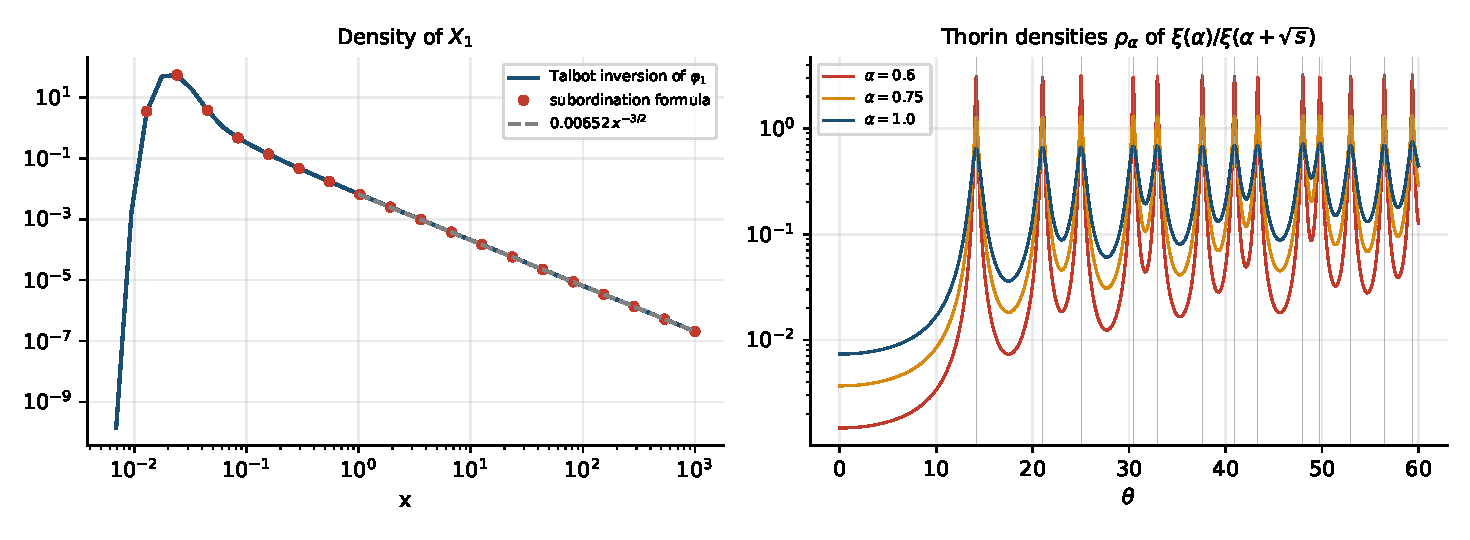
\includegraphics[width=\textwidth]{fig/bp1_density2.pdf}
\caption{Left: the density of $T_1$ by Talbot inversion of $\varphi_1$ and by the subordination formula \eqref{bp:eq:density}, with the tail $0.00652\,x^{-3/2}$. Right: the densities $v_\alpha/\pi$ at the basepoints $\alpha=0.6$, $0.75$ and $1$, with the ordinates of the zeros; they sharpen onto the zeros as $\alpha$ decreases, and for $\alpha<1$ they are Thorin densities of $T_\alpha$ only if no zero lies to the right of the line $\re s=\alpha$. The plots write $X_1$ for $T_1$, $\rho_\alpha$ for $v_\alpha/\pi$ and $s$ for $u$. Drawn by \texttt{figs2.py}.}
\label{bp:fig:density2}
\end{figure}

\label{bp:sec:planar}The Cauchy kernels of Proposition~\ref{bp:prop:thorin} and the stable one half subordinator of Theorem~\ref{bp:thm:sub} are both laws of planar Brownian motion at the moment it first reaches a line. Let $B=(B^1,B^2)$ be a planar Brownian motion started at a zero $\rho=\beta+i\gamma$, identified with the point $(\beta,\gamma)$, and let $H$ be the first time $B^1$ reaches the line $\re s=1$, a distance $1-\beta$ away, that is, the first passage time $H_{1-\beta}$ of the one dimensional Brownian motion $B^1-\beta$. Then $B^2_H$ has the Cauchy law with centre $\gamma$ and width $1-\beta$, which is the harmonic measure of the half plane, and $H$ has Laplace transform $e^{-(1-\beta)\sqrt{2u}}$, the stable one half law. So, exactly,
\[
\rho_{1/2}(\theta)\,d\theta=\sum_\rho P\big(B^2_H\in d\theta\mid B_0=\rho\big).
\]
The times $H$ have the same stable one half law, up to scale, as the stable part of the subordinator $\sigma$ in Theorem~\ref{bp:thm:sub}; the correspondence is of type rather than of scale, since in the theorem the stable part runs per unit of local time $\widetilde T$ rather than per unit of distance.

\subsection{The exact Brownian boundary and Wald's identity}\label{bp:sec:rs1}

The inverse first passage question asks for a boundary $b$ such that the first time $H_b=\inf\{t>0:B_t\ge b(t)\}$ at which a standard Brownian motion started at zero crosses $b$ has the law of $T_1$. A deterministic curved boundary always exists. Anulova proved this for two sided symmetric boundaries \cite{Anulova80}, and Chen, Cheng, Chadam and Saunders for one sided boundaries when the survival function is continuous and positive \cite[Theorem 1]{CCCS11}. By the theorems of Ekstr\"om and Janson \cite[Theorems 2.3, 8.2 and 9.2]{EkstromJanson16}, every law on $(0,\infty)$ is the law of $H_b$ for a lower semicontinuous boundary $b$, which is continuous on every interval where the density of the law is bounded below by a positive constant; when that holds on every compact subinterval of $(0,\infty)$, $b$ is the unique continuous solution of the Volterra equation \eqref{eq:ch19:volterra} with $\liminf_{t\downarrow0}b(t)\ge0$. The density \eqref{bp:eq:density} of $T_1$ is continuous and positive on $(0,\infty)$, so the boundary of $T_1$ is continuous there, and it can be computed from the law of $T_1$ alone through \eqref{eq:ch19:volterra}, with $f$ the density of $T_1$, used in the complementary form of Section~\ref{sec:ch19:zones}, with $P(T_1>t)$ in place of $P(T>t)$, once the survival probability falls below one half; \texttt{rs1.py} solves it. We computed the distribution function of $T_1$ by Talbot inversion of $\varphi_1(u)/u$ for $t<0.03$, where $T_1$ is super flat, and by the subordination representation of Theorem~\ref{bp:thm:sub} beyond, in the form
\[
P(T_1>t)=\E\Big[\mathbf 1\{\widetilde T\ge t\}+\mathbf 1\{\widetilde T<t\}\Big(2\mathcal N\Big(\frac{\widetilde T}{\sqrt{2(t-\widetilde T)}}\Big)-1\Big)\Big],
\]
with $\mathcal N$ the standard normal distribution function, as in Section~\ref{sec:ch19:zones}. This form is smooth and gives the survival function to relative accuracy even at $t=100$, where $\sqrt t\,P(T_1>t)=0.013037$ against the limit $0.013030$. As at the centre, the boundary is computed over the three zones of Section~\ref{sec:ch19:zones}.

In the small time zone the law of $T_1$ near the origin is that of the tilted centre clock, and the boundary starts from the reflection level $0.505$ at $t=0.009$. In the bulk, from $t=0.011$ to $t=0.05$, the boundary falls steeply, to $0.363$ at $t=0.012$ and $0.111$ at $t=0.02$. Here the tangent approximation, taken in its density form, equates the first passage density of the tangent line with the density of $T_1$, where the boundary of Roberts and Shortland \cite{RS95} in Section~\ref{sec:ch19:tangent} equates hazards. Its solution, the boundary $b$ with $(b-tb')(2\pi t^3)^{-1/2}e^{-b^2/2t}=f(t)$ computed by \texttt{rs1c.py}, agrees with the exact boundary to $10^{-4}$ at $t=0.012$ and to $1.5\times10^{-3}$ at $t=0.02$.

The right tail is where the basepoint one differs completely from the centre. At the centre the survival function is exponential and the boundary is asymptotically linear with slope $-\sqrt2\gamma_1$ (Section~\ref{sec:ch19:zones}). At the basepoint one the survival function is the stable one half tail $0.01303\,t^{-1/2}$, and a Brownian motion survives that long only below a boundary that stops moving. The exact boundary flattens at the level $b_\infty=-0.19277$: it stays within $10^{-3}$ of this level from $t=0.056$ on and within $10^{-4}$ from $t=1.2$ on, up to the end of the computation at $t=100$; that $b_\infty=\lim_{t\to\infty}b(t)$ is observed, not proved. The tangent approximation fails here: it overshoots downward, to $-0.332$ at $t=0.05$ against the exact $-0.188$, and has no solution beyond $t=0.091$. It treats the crossing density at time $t$ as if the path had just started, so a flat boundary at level $a$ would have to produce the density $a\,(2\pi)^{-1/2}t^{-3/2}$, forcing $a=\sqrt{2\pi}\times0.00652=0.0163>0$; but by the time the tail is reached the tangent boundary is already negative, and a negative linear boundary can only produce an exponential tail.

The positive number $0.0163$ does appear in the exact picture, in a different role. Optional stopping for the martingale $B_{t\wedge H_b}$ gives $\E[b(H_b)\mathbf 1\{H_b\le t\}]=-\E[B_t\mathbf 1\{H_b>t\}]$, and once the boundary is flat, a survivor at depth $y$ below it survives a further time $r$ with probability about $y\sqrt{2/(\pi r)}$. The next lemma makes the matching of these two facts exact. For a continuous monotone boundary that is positive at $0$ the limit is Theorem~2 of Novikov \cite{Novikov96}; the lemma assumes boundedness in place of monotonicity.

\begin{lemma}\label{bp:lem:wald}
Let $b$ be continuous on $(0,\infty)$ and bounded on $[1,\infty)$, and let $H_b=\inf\{t>0:B_t\ge b(t)\}$ be positive almost surely. Then $b(H_b)=B_{H_b}$ is integrable and $\sqrt t\,P(H_b>t)\to\sqrt{2/\pi}\,\E\,b(H_b)$ as $t\to\infty$.
\end{lemma}

\begin{proof}
Since $b$ is bounded above on $[1,\infty)$ and $\limsup_tB_t=\infty$, $H_b$ is finite, and $B_{H_b}=b(H_b)$ by continuity. Choose $u_0>0$ with $P(H_b>u_0)>0$; on that event $b>B$ on $(0,u_0]$, so $b$, which is also continuous on $[u_0,1]$ and bounded on $[1,\infty)$, is bounded below on $(0,\infty)$, say by $-K$. Optional stopping gives $A(s)=\E[b(H_b)\mathbf 1\{H_b\le s\}]=-\E[B_s\mathbf 1\{H_b>s\}]$. Fix $s\ge1$, let $c_1$ and $c_2$ be the infimum and the supremum of $b$ on $[s,\infty)$, and let $g(y,\tau)=(2\mathcal N(y/\sqrt\tau)-1)^+$, the probability that a Brownian motion started at zero stays below the level $y$ up to time $\tau$. By the Markov property at time $s$, on $\{H_b>s\}$ the conditional probability of $\{H_b>t\}$ given the path up to time $s$ lies between $g(c_1-B_s,t-s)$ and $g(c_2-B_s,t-s)$, and $c_2-B_s>0$ there. Since $\sqrt t\,g(y,t-s)\to\sqrt{2/\pi}\,y^+$ as $t\to\infty$, and $\sqrt t\,g(y,t-s)\le2y^+$ for $t\ge2s$, dominated convergence and $y^+\ge y$ give
\[
\begin{aligned}
\liminf_{t\to\infty}\sqrt t\,P(H_b>t)&\ge\sqrt{\tfrac2\pi}\big(c_1P(H_b>s)+A(s)\big),\\
\limsup_{t\to\infty}\sqrt t\,P(H_b>t)&\le\sqrt{\tfrac2\pi}\big(c_2P(H_b>s)+A(s)\big).
\end{aligned}
\]
The upper bound at $s=1$ and the lower bound at every $s$ bound $A(s)$ uniformly, so, since $b(H_b)\ge-K$, monotone convergence makes $b(H_b)$ integrable with $A(s)\to\E\,b(H_b)$. As $s\to\infty$, $c_1$ and $c_2$ stay bounded and $P(H_b>s)\to0$, so both bounds tend to $\sqrt{2/\pi}\,\E\,b(H_b)$.
\end{proof}

The exact boundary of $T_1$ is continuous; its boundedness on $[1,\infty)$, which the lemma needs, is observed, not proved. Granting it, the lemma and the tail \eqref{bp:eq:tail} give
\[
\E\,b(T_1)=\lim_{t\to\infty}\E\big[(b_\infty-B_t)\mathbf 1\{H_b>t\}\big]=\sqrt{\frac\pi2}\times\frac{\sum_\rho\rho^{-1}}{\sqrt\pi}=\frac{1}{\sqrt2}\sum_\rho\frac1\rho=0.0163311 ,
\]
the first equality by optional stopping, since $P(H_b>t)\to0$. So, if the boundary is bounded on $[1,\infty)$, Wald's identity $\E B_{H_b}=0$, which holds for every crossing time of finite mean, fails here, and the defect is exactly $\sum_\rho\rho^{-1}/\sqrt2$. Numerically, integrating the computed boundary against the law of $T_1$ gives $\E\,b(T_1)=0.0163370$. The defect is also the level of the stable summand of $T_1$: since $\E e^{-uH_a}=e^{-a\sqrt{2u}}$, the variable $S$ of Proposition~\ref{bp:prop:v1min} has the law of the first passage time $H_{b_1/\sqrt2}$ (Section~\ref{ri:sec:kill}).

We simulated $1.5\times10^5$ Brownian paths against the exact boundary on $[0,1]$, with a Brownian bridge crossing correction, using \texttt{rs1d.py}. The Kolmogorov distance between the simulated and the exact survival functions is $0.0019$, at the level of the Monte Carlo noise. Figure~\ref{bp:fig:rs1}, drawn by \texttt{figs5.py}, shows the boundary in its three zones and the survival check.

\begin{figure}[htbp]
\centering
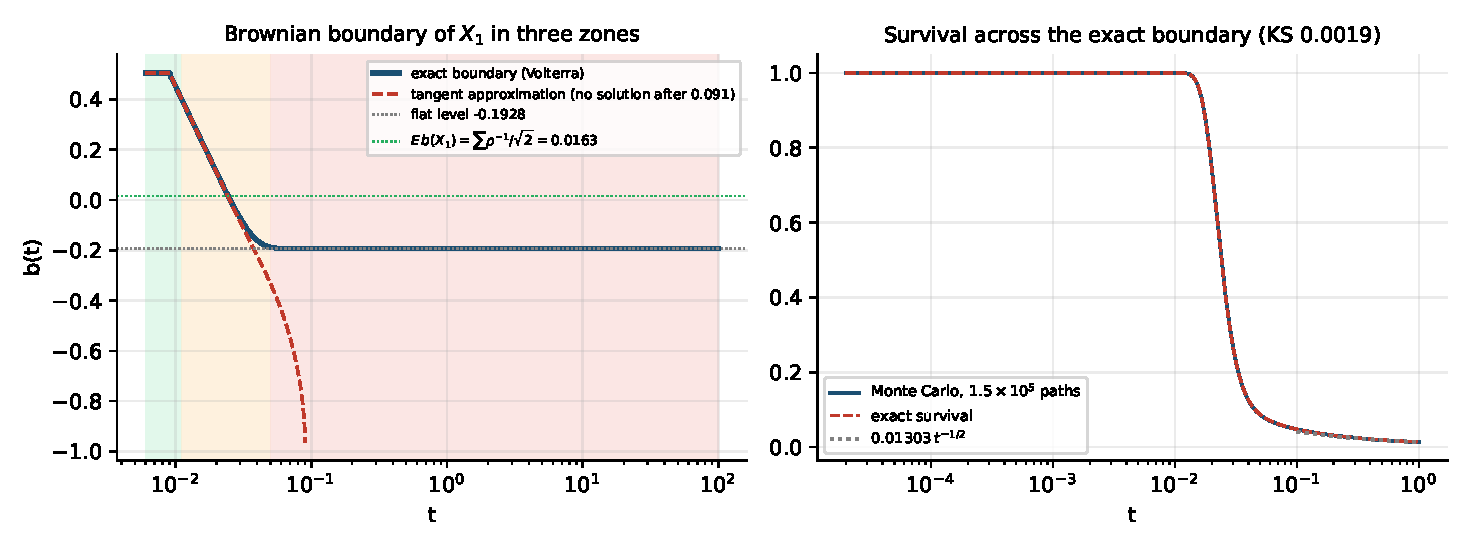
\includegraphics[width=\textwidth]{fig/bp1_rs1.pdf}
\caption{Left: the exact Brownian boundary of $T_1$, written $X_1$ in the plot, from the Volterra equation over the three zones of Section~\ref{sec:ch19:zones} (shaded: small time, bulk, right tail), the tangent approximation, which has no solution beyond $t=0.091$, the flat level $-0.19277$, and the value $\E\,b(T_1)=\sum_\rho\rho^{-1}/\sqrt2=0.0163$. Right: survival of $1.5\times10^5$ simulated Brownian paths across the exact boundary against the exact survival function of $T_1$ and the tail $0.01303\,t^{-1/2}$; the Kolmogorov distance is $0.0019$.}
\label{bp:fig:rs1}
\end{figure}

\subsection{Every basepoint above the centre}\label{bp:sec:alpha}

Nothing in Theorem~\ref{bp:thm:sub} is special to the basepoint one. Since $(\alpha-\frac12+\sqrt u)^2=(\alpha-\frac12)^2+u+2(\alpha-\frac12)\sqrt u$, the same computation applies at every basepoint to the right of the centre.

\begin{theorem}\label{bp:thm:alpha}
For every $\alpha>\frac12$, with no hypothesis on the zeros (the existence of the centre clock, Theorem~\ref{thm:ch12:idsd}, uses the verification of RH below height $1000$), $\varphi_\alpha(u)=\xi(\alpha)/\xi(\alpha+\sqrt u)$ is the Laplace transform of $T_\alpha\stackrel{d}{=}\sigma^{(\alpha)}_{\widetilde T_\alpha}$, where $\widetilde T_\alpha$ is the centre clock tilted by $e^{-(\alpha-\frac12)^2T}$ and $\sigma^{(\alpha)}$ is an independent subordinator with exponent $u+2(\alpha-\frac12)\sqrt u$, that is $T_\alpha\stackrel{d}{=}\widetilde T_\alpha+H_{\sqrt2(\alpha-\frac12)\widetilde T_\alpha}$. The law has infinite mean and $P(T_\alpha>x)\sim\frac{\xi'}{\xi}(\alpha)\,(\pi x)^{-1/2}$. The variable $T_\alpha$ is a GGC if and only if no zero has $\beta>\alpha$, in particular for every $\alpha\ge1$, and when every zero has $\beta<\alpha$ its Thorin density in the chart $\theta=\sqrt z$ is $\frac1\pi\sum_\rho(\alpha-\beta)/((\alpha-\beta)^2+(\theta-\gamma)^2)$.
\end{theorem}

\begin{proof}
The subordination is the computation of Theorem~\ref{bp:thm:sub} with $\frac14$ replaced by $(\alpha-\frac12)^2$ and $\sqrt u$ by $2(\alpha-\frac12)\sqrt u$, and $H_a$ has exponent $a\sqrt{2u}$ with $a=\sqrt2(\alpha-\frac12)\ell$. The tail follows as in Section~\ref{bp:sec:thorin} from $\varphi_\alpha(u)=1-\frac{\xi'}{\xi}(\alpha)\sqrt u+O(u)$. The Thorin density and the GGC criterion are the threshold theorem, Theorem~\ref{thm:poisson}: when every zero has $\beta<\alpha$ each Cauchy term is positive, and a zero with $\beta>\alpha$ puts a pole of $\varphi_\alpha$ at the point $(\rho-\alpha)^2$ of $\cut$ (its principal root is $\rho-\alpha$, since $\re(\rho-\alpha)>0$), where the Laplace transform of a GGC is holomorphic, whatever the sign of the density near its ordinate (Remark~\ref{rem:ch2:oneline}). In the boundary case, when some zero has $\beta=\alpha$ and none has $\beta>\alpha$, every zero has $\beta<\alpha'$ for $\alpha'>\alpha$, so $T_{\alpha'}$ is a GGC; as $\alpha'\downarrow\alpha$, $\varphi_{\alpha'}\to\varphi_\alpha$ pointwise on $[0,\infty)$, so $T_{\alpha'}\to T_\alpha$ in law, and $T_\alpha$ is a GGC by the closure theorem of Section~\ref{sec:weak:limits}. There the Cauchy kernel of a zero $\alpha+i\gamma$, $\gamma>0$, of multiplicity $m$ becomes an atom: with its conjugate it contributes the factor $(1+u/\gamma^2)^{-m}$ to $\varphi_\alpha$, a Thorin atom of mass $m$ at $z=\gamma^2$.
\end{proof}

\begin{corollary}\label{bp:cor:levyalpha}
Let $\alpha>\frac12$ and $a=\alpha-\frac12$. Then $T_\alpha$ is infinitely divisible, with no drift and L\'evy measure $W_\alpha(x)\,dx/x$, where
\begin{align*}
W_\alpha(x)&=\frac{ax}{\sqrt\pi}\int_0^x(x-s)^{-3/2}e^{-a^2xs/(x-s)}\,W(s)\,ds\\
&=\E\Big[(1+4xV)^{-1/2}\,W\Big(\frac x{1+4xV}\Big)\Big],
\end{align*}
with $V=a^2/(2Z^2)$ and $Z$ standard normal. Hence $W_\alpha>0$ and $W_\alpha'<0$ on $(0,\infty)$, so that $T_\alpha$ is self decomposable; and on every interval $(0,T]$ on which $W$ is completely monotone, so is $W_\alpha$.
\end{corollary}

\begin{proof}
By Theorem~\ref{bp:thm:alpha}, $T_\alpha$ is the subordinator $\sigma^{(\alpha)}_s=s+H_{\sqrt2as}$ evaluated at the independent time $\widetilde T_\alpha$, which is infinitely divisible with no drift and L\'evy measure $e^{-a^2s}W(s)\,ds/s$, and $H_{\sqrt2as}$ has the density $(as/\sqrt\pi)y^{-3/2}e^{-a^2s^2/y}$. By Bochner's subordination \cite[Theorem 30.1]{Sato99}, $T_\alpha$ is infinitely divisible with no drift and L\'evy measure $\int_0^\infty P(\sigma^{(\alpha)}_s\in dx)\,e^{-a^2s}W(s)\,ds/s$, which, since $a^2s^2/(x-s)+a^2s=a^2xs/(x-s)$, is $W_\alpha(x)\,dx/x$ with the first form of $W_\alpha$. The substitution $s=x/(1+4xv)$ turns the integral into an average against the density $\frac a{2\sqrt\pi}v^{-3/2}e^{-a^2/4v}$ of $V$, which is the second form. There the derivative in $x$ of $(1+4xv)^{-1/2}W(x/(1+4xv))$ is $-2v(1+4xv)^{-3/2}W+(1+4xv)^{-5/2}W'$, negative because $W>0$ and $W'<0$ (Theorem~\ref{thm:ch12:idsd}), and differentiation under the average is legitimate, because $W^{(n)}(s)=O(s^{-n-1/2}\log(1/s))$ as $s\to0$ makes every derivative in $x$ of the integrand $O(\log(1+V))$ on compact subsets of $(0,\infty)$, and $\E\log(1+V)<\infty$. Finally, $x\mapsto x/(1+4xv)$ has a completely monotone derivative and maps $(0,T]$ into itself, and $(1+4xv)^{-1/2}$ is completely monotone, so Fa\`a di Bruno's formula and Leibniz's rule carry complete monotonicity of $W$ on $(0,T]$ to every term of the average.
\end{proof}

With Theorem~\ref{thm:ch12:cmint}, $W_\alpha$ is therefore completely monotone on $(0,1.29]$ for every $\alpha>\frac12$. When no zero has real part above $\alpha$, in particular for every $\alpha\ge1$, $T_\alpha$ is a GGC and $W_\alpha$ is the Laplace transform $k_\alpha$ of its Thorin measure (Section~\ref{pm:sec:wg}); when some zero has real part above $\alpha$, $T_\alpha$ is not a GGC, so $W_\alpha$ is not completely monotone on $(0,\infty)$, although it is on $(0,1.29]$.

Table~\ref{bp:tab:alpha}, computed by \texttt{improve.py}, and the right panel of Figure~\ref{bp:fig:density2} give the constants and the densities for three basepoints. As $\alpha\downarrow\frac12$ the tail constant $\frac{\xi'}{\xi}(\alpha)/\sqrt\pi$ tends to zero, because $\xi'(\frac12)=0$, and the law acquires the finite mean $\sum_ka_k^{-1}$ of the centre clock; at the same time the subordinator tends to pure drift and the Cauchy widths to $\frac12-\beta$, which is where RH is decided.

\begin{table}[htbp]
\centering\small
\begin{tabular}{cccc}
\toprule
$\alpha$ & $\frac{\xi'}{\xi}(\alpha)$ & tail constant $\frac{\xi'}{\xi}(\alpha)/\sqrt\pi$ & $\min_{[0,60]}\rho_{\alpha-1/2}$\\
\midrule
0.6 & 0.00462092 & 0.002607 & 0.00147\\
0.75 & 0.01155134 & 0.006517 & 0.00368\\
1 & 0.02309571 & 0.013030 & 0.00735\\
\bottomrule
\end{tabular}
\caption{Basepoints above the centre: the drift $\frac{\xi'}{\xi}(\alpha)$, the tail constant of $T_\alpha$, and the minimum on $[0,60]$, attained at the origin, of the density $\rho_{\alpha-1/2}=v_\alpha/\pi$, the Thorin density of $T_\alpha$ when every zero lies to the left of the line $\re s=\alpha$. At $\alpha=1$ the minimum at the origin holds at every height (Proposition~\ref{bp:prop:v1min}), as it does at every $\alpha\ge1$ (Proposition~\ref{bp:prop:valpha}); for $\frac12<\alpha<1$ the minimum at the origin holds on the verified window $|\theta|\le3\times10^{12}-1.21$ (Theorem~\ref{thm:dbeta:minall}(ii)), and at every height for every such $\alpha$ it is equivalent to RH (part (vi) of that theorem).}
\label{bp:tab:alpha}
\end{table}

\subsection{Boundaries across the basepoints}\label{bp:sec:across}

We solved the Volterra equation \eqref{eq:ch19:volterra} \cite{Peskir02} at $\alpha=0.6$ and $0.75$, with the law of $T_\alpha$ from Theorem~\ref{bp:thm:alpha}. As at the basepoint one, the distribution function comes from Talbot inversion of $\varphi_\alpha(u)/u$ for $t<0.03$ and from the subordination identity beyond, here with $3\times10^5$ draws of $\widetilde T_\alpha$, made under RH as a sum of exponential variables over the first $200$ zeros and a gamma variable with the mean and variance of the remaining terms. The bottom left panel of Figure~\ref{pm:fig:paths} in Section~\ref{ch:sato} draws the four boundaries together.

In the small time zone and the bulk the boundaries at the different basepoints are close: they start near the reflection level $0.50$, and at $t=0.02$ they are at $0.072$ for the centre and at $0.080$, $0.092$ and $0.111$ for $\alpha=0.6$, $0.75$ and $1$. They differ in the right tail. At the centre the survival function is exponential with rate $\gamma_1^2$, and the boundary is asymptotically linear with slope $-\sqrt2\gamma_1=-19.99$ and the logarithmic correction $\frac{3}{2\sqrt2\gamma_1}\log t$; the slope of the computed boundary over $[0.2,0.3]$ is $-19.77$ (Section~\ref{sec:ch19:zones}). Above the centre the exact boundaries flatten: each stays within $0.011$ of its level at $t=100$, the end of the computation, from $t=0.1$ on, and within $10^{-3}$ from $t=1$ on. As $\alpha\downarrow\frac12$ the flat level moves down, towards the linear boundary of the centre.

The Wald type identity of Section~\ref{bp:sec:rs1} extends to every basepoint above the centre. The density of $T_\alpha$ is again continuous and positive on $(0,\infty)$, so its boundary is continuous \cite[Theorem 8.2]{EkstromJanson16}, and as computed it is bounded up to $t=100$. Granting boundedness at infinity, which here too is observed, not proved, Lemma~\ref{bp:lem:wald} and the stable tail $P(T_\alpha>t)\sim b_\alpha(\pi t)^{-1/2}$ of Theorem~\ref{bp:thm:alpha} give $\E\,b(T_\alpha)=b_\alpha/\sqrt2$, so Wald's identity $\E B_{H_b}=0$ fails by exactly $b_\alpha/\sqrt2$. Table~\ref{bp:tab:across} compares the identity and the tail constant with the computed values; all six pairs agree to within $6\times10^{-4}$ in relative terms. The reason given in Section~\ref{bp:sec:rs1} for the failure of the tangent approximation in the right tail holds at every basepoint above the centre.

\begin{table}[htbp]
\centering\small
\begin{tabular}{cccccc}
\toprule
$\alpha$ & flat level & $\E\,b(T_\alpha)$ & $b_\alpha/\sqrt2$ & $\sqrt{100}\,P(T_\alpha>100)$ & $b_\alpha/\sqrt\pi$\\
\midrule
0.6 & $-0.33384$ & 0.0032687 & 0.0032675 & 0.0026083 & 0.0026071\\
0.75 & $-0.25537$ & 0.0081710 & 0.0081680 & 0.0065203 & 0.0065171\\
1 & $-0.19277$ & 0.016337 & 0.016331 & 0.013037 & 0.013030\\
\bottomrule
\end{tabular}
\caption{Exact Brownian boundaries above the centre: the flat level, the mean boundary value $\E\,b(T_\alpha)$ at the crossing, obtained by integrating the computed boundary against the law of $T_\alpha$, against the Wald type identity, and the computed $\sqrt{100}\,P(T_\alpha>100)$ against the tail constant of Theorem~\ref{bp:thm:alpha}. Computed by \texttt{bnd\_alpha.py} for $\alpha=0.6$ and $0.75$ and by \texttt{rs1.py} for $\alpha=1$.}
\label{bp:tab:across}
\end{table}

\chapter{The critical strip and Riesz's criterion}\label{chap:strip}

Chapter~\ref{chap:basepoint} read the reciprocal Xi function at a basepoint $\alpha$ as a Laplace transform on the half line, $\varphi_\alpha(u)=\xi(\alpha)/\xi(\alpha+\sqrt u)$ for $u\ge0$. At the basepoint one its Thorin measure is the Poisson smoothing of the zeros and its L\'evy form carries the primes, and by Theorem~\ref{bp:thm:alpha} it is, for every $\alpha>\frac12$ and with no hypothesis, the Laplace transform of a positive random variable $T_\alpha$ obtained by subordinating the centre clock. The same function has two further readings, as the characteristic function of a normal scale mixture and through the completeness of the translates of the tilted P\'olya kernels. Both run across the whole critical strip, not only to the right of the zeros, and so show how much of what holds with no hypothesis at the basepoint one survives inside the strip. Section~\ref{ch:strip} develops the two readings in turn and ends with Riesz's criterion, which reads the zero free half planes through growth rather than completeness. Section~\ref{ch:riesz} writes that criterion in the language of the clocks, where it becomes the statement that every $T_\alpha$ with $\alpha>\frac12$ is a GGC, and shows why none of the resulting representations of its coefficients supplies the growth bound that the criterion needs. Section~\ref{sec:sqfree} turns to the squarefree integers, whose Dirichlet series $\zeta(s)/\zeta(2s)$ carries the same reciprocal $1/\zeta(2s)$: the constant of $\sum_{n\le x}\mu(n)^2/n$ is a combination of two tilted P\'olya means, and smoothing the count by a gamma law gives criteria for RH of the same kind as Riesz's.

For the scale mixtures and the completeness statements, as for the Thorin measure and the L\'evy form in Chapter~\ref{chap:basepoint}, what is unconditional at the basepoint one extends to every basepoint to the right of the line $\re s=\alpha$, for a given $\alpha<1$, exactly when no zero lies to the right of that line; required for every $\alpha>\frac12$, this is RH. Chapters~\ref{chap:basepoint} to \ref{chap:almost} prove no new zero free region.

\section{Normal scale mixtures and completeness across the strip}\label{ch:strip}

The first of the two readings evaluates the Laplace transform $\varphi_\alpha$ at $u^2$. Since $\varphi_\alpha(u^2)=\xi(\alpha)/\xi(\alpha+|u|)$, the reciprocal of $\xi$ along the real axis is a characteristic function, that of a normal scale mixture, at every basepoint and with no hypothesis (Section~\ref{sm:sec:cf}); what the zeros decide is the class of the law. The sine squared lemma turns its L\'evy form in $|u|$ into a Thorin form in $u^2$ (Section~\ref{sm:sec:thorin}), and the law is an extended generalised gamma convolution at and to the right of the basepoint one, at a basepoint inside the strip exactly when the half plane to its right is free of zeros, at the centre exactly when RH holds, and unconditionally up to a remainder of relative size $\log T_0/T_0$, where $T_0=3\times10^{12}$ is the height to which the zeros have been verified (Section~\ref{sm:sec:strip}). Its L\'evy density, multiplied by $|y|$, is the Laplace transform of the Thorin density, a Poisson trace of the zeros that is tied to the heat trace $W$ by stable one half subordination with no hypothesis (Section~\ref{sm:sec:poisson}). Section~\ref{sec:biane:cm} writes the complete monotonicity of the Poisson trace at the centre, which is RH, as conditions indexed by an order $n$ and a point $y$, proves those with $n<T_0(\pi-y)$ with no hypothesis, and compares the trace with that of P\'olya's Bessel function, whose complete monotonicity is a theorem.

The second reading is completeness. The Fourier transform of P\'olya's kernel tilted to the basepoint $\alpha$ is $\xi(\alpha+i\theta)$, so by Wiener's closure theorem the translates of the tilted kernel are complete in $L^1(\R)$ exactly when no zero lies on the line $\re s=\alpha$. The zero free half planes of Chapter~\ref{chap:basepoint} thus become completeness statements, with an explicit obstruction at the centre and an explicit cost of approximation above it (Section~\ref{wr:sec:wiener}). Salem's criterion is the same statement for a Fermi Dirac kernel (Section~\ref{wr:sec:salem}), and the criteria of Riesz and of Nyman and Beurling are its growth and multiplicative counterparts (Section~\ref{wr:sec:riesz}).

We keep the notation of Chapter~\ref{chap:basepoint}: $T$ is the centre clock and $T_{1/2}=T$, $\widetilde T_\alpha$ is the centre clock tilted by $e^{-(\alpha-\frac12)^2T}$, $H_a$ is the first passage time of a standard Brownian motion to the level $a$, $b_\alpha=\frac{\xi'}{\xi}(\alpha)$ and $v_\alpha(\theta)=\re(\xi'/\xi)(\alpha+i\theta)$. When every zero lies to the left of the line $\re s=\alpha$, the Thorin density of $T_\alpha$ in the chart $\theta=\sqrt z$ is $v_\alpha/\pi$, the density $\rho_{\alpha-1/2}$ of \eqref{eq:rho} (Theorem~\ref{thm:poisson}); when a zero lies to the right of that line, $T_\alpha$ is not a GGC and $v_\alpha/\pi$ is not a Thorin density for it (Proposition~\ref{ag:prop:factor}). Throughout, $Z$ is a standard normal variable independent of everything else. The scripts are in the folders \texttt{basepoint\_one/scale\_mixture} and \texttt{basepoint\_one/wiener} of the archive, and we name them at each table and figure.

\subsection{The reciprocal on the real axis is a characteristic function}\label{sm:sec:cf}

Evaluating a Laplace transform at the square of a real variable produces the characteristic function of a normal scale mixture: if $X\ge0$ is independent of $Z$, then $\E e^{iu\sqrt{2X}Z}=\E e^{-u^2X}$ for real $u$. The centre clock $T$ of \cite{P17}, with $\E e^{-uT}=\xi(\frac12)/\xi(\frac12+\sqrt u)$, is a positive random variable, infinitely divisible and self decomposable with no hypothesis (Theorem~\ref{thm:ch12:idsd}, whose proof uses the verification of RH below height $1000$). For $\alpha>\frac12$, Theorem~\ref{bp:thm:alpha} writes $T_\alpha\stackrel d=\sigma^{(\alpha)}_{\widetilde T_\alpha}\stackrel d=\widetilde T_\alpha+H_{\sqrt2(\alpha-\frac12)\widetilde T_\alpha}$, where $\sigma^{(\alpha)}$ is an independent subordinator with Laplace exponent $u+2(\alpha-\frac12)\sqrt u$, the inverse local time at zero of a sticky Brownian motion. So $T_\alpha$ also exists with no hypothesis, and with $X=T_\alpha$ the evaluation gives the following.

\begin{proposition}\label{sm:prop:cf}
For every $\alpha\ge\frac12$ the function $u\mapsto\varphi_\alpha(u^2)=\xi(\alpha)/\xi(\alpha+|u|)$ is the characteristic function of $Y_\alpha=\sqrt{2T_\alpha}\,Z$. The law of $Y_\alpha$ is symmetric, unimodal and infinitely divisible with no hypothesis. At the centre it has variance $2\E T=2\sum_ka_k^{-1}=0.046210$. For $\alpha>\frac12$ its characteristic function has a corner at the origin, $\xi(\alpha)/\xi(\alpha+|u|)=1-b_\alpha|u|+O(u^2)$, so $Y_\alpha$ lies in the domain of attraction of the Cauchy law, with $P(|Y_\alpha|>y)\sim2b_\alpha/(\pi y)$ as $y\to\infty$.
\end{proposition}

\begin{proof}
The first statement is the evaluation $\E e^{iu\sqrt{2X}Z}=\E e^{-u^2X}$ with $X=T_\alpha$. Symmetry and unimodality hold for every normal scale mixture, which is a mixture of centred normal laws. The tilt $\widetilde T_\alpha$ of the infinitely divisible law of $T$ is infinitely divisible, with L\'evy measure $e^{-(\alpha-\frac12)^2t}W(t)\,dt/t$, and a subordinator run for an independent infinitely divisible time is infinitely divisible, because a Bernstein function composed with a Bernstein function is again one \cite[Corollary 3.8]{boSSV}. So $T_\alpha$ is infinitely divisible, and $Y_\alpha$, which is a Brownian motion run for the independent time $2T_\alpha$, is infinitely divisible for the same reason. At the centre $\xi'(\frac12)=0$, so $\xi(\frac12)/\xi(\frac12+|u|)=1-\E T\,u^2+O(u^4)$, with $\E T=\sum_ka_k^{-1}$ by \eqref{eq:ch2:hadamard}. For $\alpha>\frac12$ the expansion follows from $\xi(\alpha+|u|)=\xi(\alpha)(1+b_\alpha|u|+O(u^2))$. The tail comes from that of $T_\alpha$: by Theorem~\ref{bp:thm:alpha}, $P(T_\alpha>t)\sim b_\alpha(\pi t)^{-1/2}$ as $t\to\infty$, so that, since $P(T_\alpha>t)\le1$, also $P(T_\alpha>t)\le Kt^{-1/2}$ for all $t>0$ and some constant $K$. Conditioning on $Z$, $yP(|Y_\alpha|>y)=\E\big[yP(T_\alpha>y^2/(2Z^2)\mid Z)\big]$, and the integrand is at most $\sqrt2K|Z|$ and tends to $\sqrt{2/\pi}\,b_\alpha|Z|$ as $y\to\infty$; by dominated convergence $yP(|Y_\alpha|>y)\to\sqrt{2/\pi}\,b_\alpha\E|Z|=2b_\alpha/\pi$.
\end{proof}

At the centre $Y_{1/2}=Z\sqrt{2T}$ is the second member of the van Dantzig pair of Section~\ref{ch:clock}; it has the same variance as the P\'olya variable $X$, the first member, as the relation $\E e^{-\theta^2T}=1/\E e^{\theta X}$ requires. What RH decides is not whether $\xi(\frac12)/\xi(\frac12+|u|)$ is a characteristic function, which it always is, but which class it lies in, and that is the subject of Sections~\ref{sm:sec:thorin} and \ref{sm:sec:strip}. Table~\ref{sm:tab:mc}, computed by \texttt{comp.py}, checks the proposition by Monte Carlo, drawing $T_\alpha$ from the subordination identity with $4\times10^5$ draws. The tilted clock $\widetilde T_\alpha$ is drawn as a sum of independent exponential variables with rates $\gamma^2+(\alpha-\frac12)^2$ over the first $200$ zeros, which lie on the critical line, plus a gamma variable with the mean and variance of the remaining factors, and $H_a$ is drawn as $a^2/Z'^2$ with $Z'$ standard normal.

\begin{table}[htbp]
\centering\small
\begin{tabular}{ccccc}
\toprule
$\alpha$ & $u$ & $\E\cos(uY_\alpha)$, Monte Carlo & standard error & $\xi(\alpha)/\xi(\alpha+|u|)$\\
\midrule
0.5 & 1 & 0.977101 & 0.000053 & 0.977178\\
0.5 & 5 & 0.566634 & 0.000768 & 0.567395\\
0.75 & 1 & 0.966125 & 0.000176 & 0.965980\\
0.75 & 5 & 0.536687 & 0.000812 & 0.536769\\
1 & 1 & 0.954736 & 0.000246 & 0.954930\\
1 & 5 & 0.507781 & 0.000851 & 0.507962\\
\bottomrule
\end{tabular}
\caption{Proposition~\ref{sm:prop:cf} by simulation, computed by \texttt{comp.py}. At the centre the sample variance of $Y_{1/2}$ is $0.04637$ against $0.04621$. The Cauchy tails $y\,P(|Y_\alpha|>y)$ at $y=10$ are $0.0144$ at $\alpha=1$ and $0.0066$ at $\alpha=0.75$, against $2b_\alpha/\pi=0.0147$ and $0.0074$.}
\label{sm:tab:mc}
\end{table}

With no hypothesis the law of $Y_{1/2}$ is also self decomposable. For $0<c<1$ the self decomposability of $T$ (Theorem~\ref{thm:ch12:idsd}) gives $T\stackrel d=cT'+R_c$ with $T'\stackrel d=T$ and $R_c\ge0$ independent, and then $Y_{1/2}\stackrel d=\sqrt c\,Y'+Z'\sqrt{2R_c}$, where $Y'=Z\sqrt{2T'}$ has the law of $Y_{1/2}$ and $Z'$ is standard normal and independent of $(Z,T',R_c)$.

Under RH each factor $(1+u^2/\gamma^2)^{-1}$ of $\xi(\frac12)/\xi(\frac12+|u|)$ is a characteristic function, that of $L/\gamma$ for a standard Laplace variable $L$, and a zero off the line would break this. The quadruple $\frac12\pm\delta\pm i\gamma$, with $\gamma>0$ and $0<\delta<\frac12$, contributes to $\xi(\frac12)/\xi(\frac12+|u|)$, by \eqref{eq:ch2:hadamard}, the factor $g(u)=|1+u^2/(\gamma-i\delta)^2|^{-2}$, which is positive and integrable with $g(0)=1$, and
\[
\frac1{2\pi}\int_{\R}g(u)e^{-iux}\,du=\frac{\gamma^2+\delta^2}{4\gamma\delta}\,e^{-\gamma|x|}\big(\gamma\sin\delta|x|+\delta\cos\delta|x|\big).
\]
For $x>0$ the derivative of the right side is $-\frac{(\gamma^2+\delta^2)^2}{4\gamma\delta}e^{-\gamma x}\sin\delta x$, so its least value, attained at $x=\pi/\delta$, is $-e^{-\pi\gamma/\delta}$ times its value $(\gamma^2+\delta^2)/(4\gamma)$ at $x=0$. Since $g$ is integrable, it could only be the characteristic function of the law with this density, which is negative there. So $g$ is not a characteristic function, and $\xi(\frac12)/\xi(\frac12+|u|)$ would still be one, as $W>0$ ensures, but no longer factor by factor. The defect is tiny. Every ordinate is at least $\gamma_1$ and $\delta<\frac12$, so the least value exceeds $-9.5\times10^{-39}$, the value of the formula at $\gamma=\gamma_1$ and $\delta=\frac12$; and a zero off the line would lie above $T_0$, where $e^{-\pi\gamma/\delta}<e^{-2\pi T_0}$. The script \texttt{vdpair.py} of Section~\ref{ch:clock} computes these values and checks the transform against quadrature.

Away from the centre neither $V_\alpha$ nor $Y_\alpha$ belongs to a pair. Take $\alpha>\frac12$; for $V_\alpha$ the case $\alpha<\frac12$ follows, since $V_\alpha\stackrel d=-V_{1-\alpha}$. The tilted P\'olya variable $V_\alpha$ of Section~\ref{ch:clock} has characteristic function $\varphi(\theta)=\xi(\alpha+i\theta)/\xi(\alpha)$, and $1/\varphi(i\theta)=\xi(\alpha)/\xi(\alpha-\theta)$ exceeds $1$ for $0<\theta<2\alpha-1$, because $|\alpha-\theta-\frac12|<\alpha-\frac12$ there and $\xi(\frac12+s)=\xi(\frac12)\E\cosh(sX)$ increases with $|s|$; at $\alpha=0.75$ and $\theta=0.25$ it is $1.00145$. So it is not a characteristic function. By its Cauchy tail $Y_\alpha$ has no exponential moments, so it cannot be a first member. As a second member its partner $\varphi$ would satisfy $\varphi(i\theta)=\xi(\alpha+|\theta|)/\xi(\alpha)$, and a moment generating function finite on the whole line is analytic, while $\xi(\alpha+|\theta|)/\xi(\alpha)=1+b_\alpha|\theta|+O(\theta^2)$ has a corner at $\theta=0$, since $b_\alpha>0$ (Proposition~\ref{sm:prop:cf}). At the centre the bound by $1$ and the corner both disappear, because $\xi(\frac12-\theta)=\xi(\frac12+\theta)$ and so $b_{1/2}=0$: the functional equation is what permits the pair, and Theorem~\ref{thm:ch12:idsd} is what supplies it.

\subsection{From the L\'evy form in \texorpdfstring{$|u|$}{|u|} to the Thorin form in \texorpdfstring{$u^2$}{u2}}\label{sm:sec:thorin}

For $\alpha\ge1$ the function $\log(\xi(\alpha+s)/\xi(\alpha))$ has, for $\re s>0$, the L\'evy form \eqref{bp:eq:levyform} with $b_\alpha$ and $\Pi_\alpha$ in place of $b_1$ and $\Pi_1$, where $x\Pi_\alpha(dx)=\big(\frac{e^{-(\alpha+2)x}}{1-e^{-2x}}-e^{-(\alpha-1)x}\big)dx+\sum_n\Lambda(n)n^{-\alpha}\delta_{\log n}(dx)$ is the signed measure that Section~\ref{bp:sec:levy} gives for every basepoint $\alpha\ge1$. The integral converges absolutely for $\alpha>1$, and at $\alpha=1$ as a compensated limit, by the prime number theorem. Putting $s=|u|$ gives
\begin{equation}\label{sm:eq:levyu}
\frac{\xi(\alpha)}{\xi(\alpha+|u|)}=e^{-b_\alpha|u|}\exp\Big\{-\int_0^\infty\big(e^{-|u|x}-1+|u|x\big)\Pi_\alpha(dx)\Big\},
\end{equation}
a representation in $|u|$. The first factor is the characteristic function of a Cauchy law of scale $b_\alpha$. The second is not in L\'evy Khintchine form, because $e^{-|u|x}$ is a function of $|u|$ rather than of $u$. The sine squared lemma \eqref{eq:sin2} converts it. In the chart $\theta=\sqrt z$ and at $s=|u|$, as in the derivation of \eqref{bp:eq:conversion}, it writes $e^{-|u|x}+|u|x-1$ as $\frac{2x}\pi\int_0^\infty\log(1+u^2/\theta^2)\sin^2(x\theta/2)\,d\theta$ for $x>0$, and the drift converts through $|u|=\frac1\pi\int_0^\infty\log(1+u^2/\theta^2)\,d\theta$. Both identities follow from $\int_0^\infty\log(1+u^2/\theta^2)\cos(x\theta)\,d\theta=\pi(1-e^{-|u|x})/x$.

By Section~\ref{sec:ch3:hierarchy}, a symmetric law is an extended generalised gamma convolution (EGGC) if and only if it is the law of $Z\sqrt{2T'}$ with $T'$ a GGC independent of $Z$, and at the centre $Y_{1/2}=Z\sqrt{2T}$ is an EGGC exactly when RH holds. The next theorem carries this to every basepoint above the centre; Section~\ref{sm:sec:strip} describes the class through its characteristic functions.

\begin{theorem}\label{sm:thm:thorin}
Let $\alpha\ge1$, or more generally let $\alpha>\frac12$ be such that $\re\rho<\alpha$ for every zero $\rho$. Then
\begin{equation}\label{sm:eq:thorin}
\frac{\xi(\alpha)}{\xi(\alpha+|u|)}=\exp\Big\{-\frac1\pi\int_0^\infty\log\Big(1+\frac{u^2}{\theta^2}\Big)v_\alpha(\theta)\,d\theta\Big\},
\end{equation}
where
\[
v_\alpha(\theta)=b_\alpha+\int_0^\infty2\sin^2\Big(\frac{x\theta}2\Big)x\Pi_\alpha(dx)=\re\frac{\xi'}\xi(\alpha+i\theta)>0,
\]
the first expression being available for $\alpha\ge1$, and as the compensated limit \eqref{bp:eq:below} (in which $\varepsilon=1-\alpha$) when $\sup_\rho\re\rho<\alpha$, so $Y_\alpha$ is a symmetric EGGC with Thorin density $v_\alpha/\pi$ in the chart $\theta$. With no hypothesis on the zeros, for $\frac12<\alpha<1$ the law of $Y_\alpha$ is an EGGC if and only if $\zeta$ has no zeros with real part greater than $\alpha$, and at the centre if and only if RH holds. Under RH,
\[
\frac{\xi(\frac12)}{\xi(\frac12+|u|)}=\prod_{\gamma>0}\Big(1+\frac{u^2}{\gamma^2}\Big)^{-1},\qquad Y_{1/2}\stackrel d=\sum_k\frac{L_k}{\gamma_k},
\]
with independent standard Laplace variables $L_k$, of density $\frac12e^{-|y|}$.
\end{theorem}

\begin{proof}
For $\alpha\ge1$, insert the two identities of the lemma into \eqref{sm:eq:levyu} and exchange the order of integration, which is justified for $\alpha>1$ by absolute convergence and at $\alpha=1$ by the compensation argument of Proposition~\ref{bp:prop:levy}. This gives the first expression for $v_\alpha$, and the second is its identification, \eqref{bp:eq:conversion} at $\alpha=1$, which is Proposition~\ref{bp:prop:sin2} of Section~\ref{bp:sec:sin2}, and \eqref{eq:split} for $\alpha>1$; for $\frac12<\alpha<1$ with $\sup_\rho\re\rho<\alpha$ the first expression holds in the compensated form \eqref{bp:eq:below} of Proposition~\ref{bp:prop:below}, in which $\varepsilon=1-\alpha$. In every case \eqref{sm:eq:thorin} is the Thorin representation of $T_\alpha$ given by Theorem~\ref{thm:poisson}, $\varphi_\alpha(u)=\exp\{-\int\log(1+u/z)\,U_\alpha(dz)\}$ with $U_\alpha$ as in \eqref{eq:Ualpha}, evaluated at $u^2$ in the chart $z=\theta^2$, and $v_\alpha>0$ because every Cauchy kernel of Proposition~\ref{prop:struct} then has positive width $\alpha-\beta$. Since $T_\alpha$ is a GGC, $Y_\alpha=Z\sqrt{2T_\alpha}$ is an EGGC. Conversely, if $Y_\alpha\stackrel d=Z\sqrt{2T'}$ with $T'$ a GGC, then $\E e^{-u^2T'}=\E e^{-u^2T_\alpha}$ for all real $u$, so $T'\stackrel d=T_\alpha$. Hence $Y_\alpha$ is an EGGC exactly when $T_\alpha$ is a GGC, which by Theorem~\ref{thm:poisson} happens exactly when $\alpha\ge\sup_\rho\re\rho$. For $\frac12<\alpha<1$ this is the absence of zeros with real part greater than $\alpha$, and at the centre, by the symmetry $\rho\mapsto1-\rho$, it is RH (Proposition~\ref{prop:rigid}). Under RH the Hadamard product \eqref{eq:ch2:hadamard} at $s=|u|$ is the product displayed, and each factor $(1+u^2/\gamma^2)^{-1}$ is the characteristic function of $L/\gamma$, as in Proposition~\ref{rz:prop:dict}(iii).
\end{proof}

The hypothesis that every zero lies to the left of the line $\re s=\alpha$ cannot be dropped from \eqref{sm:eq:thorin}. By Proposition~\ref{prop:struct}, $v_\alpha/\pi$ is, off the ordinates of the zeros on the line $\re s=\alpha$ and whatever the zeros do, the sum over the zeros with $\gamma>0$ of $P_{\alpha-\beta}(\theta-\gamma)+P_{\alpha-\beta}(\theta+\gamma)$, with $P_{-c}=-P_c$, and by the semigroup property of the Cauchy kernels $\int_0^\infty\frac{2s}{s^2+\theta^2}[P_c(\theta-\gamma)+P_c(\theta+\gamma)]\,d\theta=\frac{2(s+|c|)\operatorname{sgn}c}{(s+|c|)^2+\gamma^2}$ for $s>0$ and real $c\ne0$. Integrating in $s$ from $0$ to $|u|$ shows that a zero $\rho=\beta+i\gamma$ with $\gamma>0$ contributes to the right side of \eqref{sm:eq:thorin} the factor $((\alpha-\beta)^2+\gamma^2)/((|u|+\alpha-\beta)^2+\gamma^2)$ when $\beta<\alpha$, which is its factor in $\xi(\alpha)/\xi(\alpha+|u|)$, but the factor $((|u|+\beta-\alpha)^2+\gamma^2)/((\beta-\alpha)^2+\gamma^2)$ when $\beta>\alpha$. If no zero lies on the line $\re s=\alpha$, the integral with the signed density therefore converges and equals $\xi(\alpha)/\xi(\alpha+|u|)$ multiplied by
\[
\prod_{\beta>\alpha,\ \gamma>0}\frac{\big((|u|+\beta-\alpha)^2+\gamma^2\big)\big((|u|-\beta+\alpha)^2+\gamma^2\big)}{\big((\beta-\alpha)^2+\gamma^2\big)^2},
\]
which exceeds one for $u\ne0$ as soon as there is such a zero, since each factor equals $1+u^2(u^2+2\gamma^2-2(\beta-\alpha)^2)/((\beta-\alpha)^2+\gamma^2)^2$ and $0<\beta-\alpha<\frac12<\gamma$. The series of Proposition~\ref{prop:struct} may be integrated term by term, because the absolute value of the term of a zero integrates to $\log(((|\alpha-\beta|+|u|)^2+\gamma^2)/((\alpha-\beta)^2+\gamma^2))=O(\gamma^{-2})$. In the variable $s=|u|$, continued to the right half plane, the Poisson integral replaces the pole of $\xi(\alpha)/\xi(\alpha+s)$ at $s=\rho-\alpha$ by a zero at its mirror image $\alpha-\beta+i\gamma$ across the imaginary axis, so it cannot represent $\varphi_\alpha$, whose pole at $(\rho-\alpha)^2\in\cut$ no GGC transform can have. A zero on the line $\re s=\alpha$ contributes instead an atom of mass one at its ordinate, as every zero does at the centre under RH.

We draw out two features of \eqref{sm:eq:thorin}. The first is the Cauchy factor. The drift $b_\alpha$ becomes, through $|u|=\frac1\pi\int_0^\infty\log(1+u^2/\theta^2)\,d\theta$, the constant Thorin density $b_\alpha/\pi$, which is also the value $v_\alpha(0)/\pi$. At the basepoint one this constant is the minimum of $v_1/\pi$, attained only at $\theta=0$ (Proposition~\ref{bp:prop:v1min}), and \texttt{comp.py} confirms it on $[0,200]$. So $Y_1$ splits as an independent sum of a Cauchy variable of scale $b_1=\sum_\rho\rho^{-1}=0.0230957$ and a symmetric EGGC with Thorin density $(v_1-b_1)/\pi$ (Figure~\ref{sm:fig:strip}, left). This is the image at $u^2$ of the factorisation $T_1\stackrel d=S+T_1^\circ$ of Proposition~\ref{bp:prop:v1min} into a positive stable variable of index one half and a GGC with Thorin density $(A+Q)/\pi$: since $\E e^{-u^2S}=e^{-b_1|u|}$, the Cauchy summand is $Z\sqrt{2S}$, and the EGGC summand is $\sqrt{2T_1^\circ}$ times an independent standard normal variable, with characteristic function $e^{b_1|u|}\xi(1)/\xi(1+|u|)=\exp\{-\frac1\pi\int_0^\infty\log(1+u^2/\theta^2)(v_1-b_1)(\theta)\,d\theta\}$. The constant $b_1/\pi$ is the value at $\theta=0$ of the harmonic measure density of Section~\ref{bp:sec:planar}, the sum over the zeros of the Cauchy laws of the points where planar Brownian motions started at the zeros first reach the line $\re s=1$, and the Cauchy factor carries the whole tail of $Y_1$. The second feature is that the passage from $|u|$ to $u^2$ is exactly the passage from the L\'evy form, where the primes appear as atoms at $\log n$, to the Thorin form, where the zeros appear as the centres of the Cauchy kernels in $v_\alpha$. Table~\ref{sm:tab:thorin}, computed by \texttt{comp.py}, checks \eqref{sm:eq:thorin} with $v_\alpha$ computed from $\xi'/\xi$ on $[0,200]$ and the Weyl density $\frac1{2\pi}\log\frac\theta{2\pi}$ beyond. At $\alpha=0.75$ the formula presupposes that no zero has real part $0.75$ or more; the table is consistent with that to its accuracy, and a zero at a great height $\gamma$ would change the entries only by a relative amount of order $u^2/\gamma^2$.

\begin{table}[htbp]
\centering\small
\setlength{\tabcolsep}{4pt}
\begin{tabular}{@{}ccccc@{}}
\toprule
$u$ & Thorin form, $\alpha=1$ & $\xi(1)/\xi(1+|u|)$ & Thorin form, $\alpha=0.75$ & $\xi(0.75)/\xi(0.75+|u|)$\\
\midrule
0.5 & 0.982809 & 0.982838 & 0.988506 & 0.988520\\
1 & 0.954904 & 0.954930 & 0.965969 & 0.965980\\
2 & 0.871156 & 0.871171 & 0.891317 & 0.891317\\
5 & 0.507984 & 0.507962 & 0.536812 & 0.536769\\
20 & 0.0003491 & 0.0003487 & 0.0004116 & 0.0004110\\
\bottomrule
\end{tabular}
\caption{The Thorin form \eqref{sm:eq:thorin} against the reciprocal Xi function on the real axis, computed by \texttt{comp.py}.}
\label{sm:tab:thorin}
\end{table}

\subsection{Extended generalised gamma convolutions in the critical strip}\label{sm:sec:strip}

Thorin introduced generalised gamma convolutions to show that the Pareto law is self decomposable \cite{Thorin77a} and that the lognormal law is infinitely divisible \cite{Thorin}, and extended the idea to laws on the whole line \cite{Thorin78}. Bondesson \cite[Section 7.1]{Bondesson} calls the resulting class the extended generalised gamma convolutions, and Section~\ref{sec:ch3:hierarchy} recalls it. A symmetric law without Gaussian part is an EGGC exactly when its characteristic function has the form
\[
\exp\Big\{-\int_0^\infty\log\Big(1+\frac{u^2}{\theta^2}\Big)m(d\theta)\Big\}
\]
with a positive measure $m$ on $(0,\infty)$ that satisfies the integrability conditions of a Thorin measure in the chart $z=\theta^2$; under $z=\theta^2$ it is the Thorin measure of the mixing GGC $T'$ in the representation $Z\sqrt{2T'}$ recalled before Theorem~\ref{sm:thm:thorin}. The building blocks are the symmetric laws with characteristic function $(1+u^2/\theta^2)^{-c}$, $c>0$, which are the laws of the difference of two independent gamma variables of shape $c$ and scale $1/\theta$, and every symmetric EGGC is a weak limit of sums of independent variables of this kind. The symmetric Laplace law, $c=1$, is the block of an atom of mass one, and at the centre under RH it is the only block that occurs. Theorem~\ref{sm:thm:thorin} places $Y_\alpha$ in this framework: its candidate Thorin measure is $v_\alpha(\theta)\,d\theta/\pi$, and inside the strip the question is whether $T_\alpha$ is a GGC. That is decided by the location of the zeros and not by the sign of $v_\alpha$ on the single line $\re s=\alpha$: for $\xi$ it is not known whether positivity on one line excludes zeros to its right (Remark~\ref{rem:ch2:oneline}).

\begin{theorem}\label{sm:thm:strip}
Let $\frac12<\alpha<1$ and write $\varepsilon=\alpha-\frac12$.
\begin{enumerate}
\item With no hypothesis, $\xi(\alpha)/\xi(\alpha+|u|)$ is the characteristic function of the infinitely divisible, symmetric, unimodal law $Y_\alpha$. If every zero has real part less than $\alpha$, then \eqref{sm:eq:thorin} holds with the positive density $v_\alpha(\theta)/\pi=\frac1\pi\sum_\rho\frac{\alpha-\beta}{(\alpha-\beta)^2+(\theta-\gamma)^2}$.
\item $Y_\alpha$ is an EGGC if and only if no zero has $\beta>\alpha$, that is, if and only if $\zeta$ has no zeros in the half plane $\re s>\alpha$.
\item Let $T_0\ge2$ be a height up to which all zeros are known to lie on the critical line. Then
\[
\frac{\xi(\alpha)}{\xi(\alpha+|u|)}=\prod_{0<\gamma\le T_0}\frac{\varepsilon^2+\gamma^2}{(\varepsilon+|u|)^2+\gamma^2}\times\mathcal E_{\alpha,T_0}(u),
\]
where the finite product is the characteristic function of an EGGC whose Thorin density $\sum_{0<\gamma\le T_0}[P_\varepsilon(\theta-\gamma)+P_\varepsilon(\theta+\gamma)]$ is positive, and the remainder satisfies $|\log\mathcal E_{\alpha,T_0}(u)|\le C(|u|+u^2)\frac{\log T_0}{T_0}$ for an absolute constant $C$.
\end{enumerate}
\end{theorem}

\begin{proof}
(1) is Proposition~\ref{sm:prop:cf} and Theorem~\ref{sm:thm:thorin}, the sum being that of Proposition~\ref{prop:struct}. (2) is part of Theorem~\ref{sm:thm:thorin}: $Y_\alpha$ is an EGGC exactly when $T_\alpha$ is a GGC, and a zero with $\beta>\alpha$ puts a pole of $\varphi_\alpha$ at the point $(\rho-\alpha)^2$ of $\cut$, where the Laplace transform of a GGC is holomorphic (Theorem~\ref{thm:poisson}); the sign of $v_\alpha$ near the ordinate of that zero plays no role. (3) Group the zeros into those on the line below $T_0$ and the rest. Each pair $\frac12\pm i\gamma$ contributes the factor $\frac{\varepsilon^2+\gamma^2}{(\varepsilon+|u|)^2+\gamma^2}$, whose Thorin density is the pair of Cauchy kernels of width $\varepsilon$ at $\pm\gamma$, by the computation after Theorem~\ref{sm:thm:thorin}, and which is therefore an EGGC characteristic function. Every other zero has $|\gamma|>T_0$, and a pair $\rho,\bar\rho$ with $\gamma>T_0$ contributes $-\log(1+x)$ to $\log\mathcal E_{\alpha,T_0}(u)$, with $x=(2(\alpha-\beta)|u|+u^2)/((\alpha-\beta)^2+\gamma^2)$. Since $|\alpha-\beta|<1$, we have $x\ge-(\alpha-\beta)^2/((\alpha-\beta)^2+\gamma^2)>-\frac12$ and $|x|\le2(|u|+u^2)/\gamma^2$, so the contribution is at most $4(|u|+u^2)/\gamma^2$ in absolute value. Summing over the zeros with $\gamma>T_0$ gives at most $4(|u|+u^2)\sum_{\gamma>T_0}\gamma^{-2}$, and by partial summation this sum is at most $2\int_{T_0}^\infty N(t)t^{-3}\,dt$. For $t\ge2$ we have $N(t)\le\frac t{2\pi}\log t$: no zero has $0<\gamma<\gamma_1$, and for $t\ge\gamma_1$ the explicit bound of \cite{HSW22}, recalled in the proof of Proposition~\ref{bp:prop:v1min}, gives $N(t)\le\frac t{2\pi}\log\frac t{2\pi e}+\frac78+E(t)$, where $\frac78+E(t)<\frac t{2\pi}\log(2\pi e)$: up to $X_0$ the left side is at most $3.40$ and the right side is at least $6.38$, its value at $t=\gamma_1$, and beyond $X_0$ the left side is less than $\frac78+0.3\log t$ and the right side exceeds $0.45\,t$. So $\sum_{\gamma>T_0}\gamma^{-2}\le\frac1\pi\int_{T_0}^\infty t^{-2}\log t\,dt=\frac{1+\log T_0}{\pi T_0}\le\frac{\log T_0}{T_0}$, the last step because $T_0\ge2$, and the bound holds with $C=4$.
\end{proof}

Part (3) is the unconditional content of the EGGC property in the strip. With the verification height $T_0=3\times10^{12}$ of Platt and Trudgian \cite{PT21}, which also enters Corollary~\ref{bs:cor:uncond}, the remainder is of relative size at most $8\times10^{-11}$ for $|u|\le1$, so $Y_\alpha$ is, to that accuracy in characteristic function, an EGGC for every $\alpha>\frac12$, whether or not RH holds; Theorem~\ref{ag:thm:explicit} gives the same statement for the Laplace transform of $T_\alpha$ with explicit constants. In the same way, the negative part of $v_\alpha(\theta)/\pi$ that zeros above $T_0$ could produce is at most about $\frac{\log(T_0/2\pi)}{4\pi^2(T_0-\theta)}$, which is $2.3\times10^{-13}$ for every $\theta\le10^9$, since each such zero contributes a kernel of width less than $\frac12$ in absolute value, while the verified zeros contribute at least the minimum of their Cauchy smoothing $\sum_{0<\gamma\le T_0}[P_\varepsilon(\theta-\gamma)+P_\varepsilon(\theta+\gamma)]$; \texttt{strip.py} evaluates the bound. Grouping each zero above $T_0$ with its reflection in the critical line makes the bound unnecessary below $T_0-\frac12$: there every off line pair contributes a nonnegative term, so $v_\alpha>0$ on $[0,T_0-\frac12]$ for every $\alpha>\frac12$ (Corollary~\ref{cor:dbeta:window}). What cannot be removed is the dependence on $T_0$. A zero above $T_0$ with $\beta>\alpha$ would stop $T_\alpha$ from being a GGC, and $Y_\alpha$ from being an EGGC, whether or not it made $v_\alpha$ negative near its ordinate (Exercise~\ref{ex:ch2:line}), and no finite computation excludes such a zero (Section~\ref{sec:ch6:measure}). What can be said with no hypothesis is that the Cauchy kernels of such zeros carry a vanishing fraction of the mass of $v_\alpha/\pi$ on $[0,T]$ as $T\to\infty$ (Theorem~\ref{ag:thm:almost}).

Table~\ref{sm:tab:strip}, computed by \texttt{strip.py}, checks the product over the $1700$ computed zeros, with the Weyl density for the zeros above them, against $\xi(\alpha)/\xi(\alpha+|u|)$ at $\alpha=0.6$ and $0.75$; it agrees to within $4\times10^{-7}$, better than the Thorin integral over a finite grid. On $[0,200]$ the Thorin density is positive at both basepoints, and in both cases its minimum is at $\theta=0$ and equals the Cauchy floor $b_\alpha/\pi$: $0.0014709$ at $\alpha=0.6$ and $0.0036769$ at $\alpha=0.75$ (Figure~\ref{sm:fig:strip}, left), in agreement with the minima on $[0,60]$ in Table~\ref{bp:tab:alpha} and with the margin $0.0147\,\varepsilon$ of Section~\ref{ch:motivation}. As $\alpha$ decreases to $\frac12$ the floor tends to zero, because $\xi'(\frac12)=0$, while the densities sharpen onto the ordinates; at the centre the Cauchy component is gone, and what remains, under RH, is the sum of Laplace variables $\sum_kL_k/\gamma_k$.

\begin{table}[htbp]
\centering\small
\begin{tabular}{ccccc}
\toprule
$\alpha$ & $u$ & Thorin integral \eqref{sm:eq:thorin} & product over zeros & $\xi(\alpha)/\xi(\alpha+|u|)$\\
\midrule
0.6 & 1 & 0.9726796 & 0.9726812 & 0.9726812\\
0.6 & 5 & 0.5549761 & 0.5549190 & 0.5549193\\
0.6 & 20 & 0.0004547 & 0.0004539 & 0.0004539\\
0.75 & 1 & 0.9659691 & 0.9659798 & 0.9659798\\
0.75 & 5 & 0.5368120 & 0.5367687 & 0.5367691\\
0.75 & 20 & 0.0004116 & 0.0004110 & 0.0004110\\
\bottomrule
\end{tabular}
\caption{The EGGC representation in the strip, computed by \texttt{strip.py}: the Thorin integral over $\theta\le200$ plus the Weyl tail, and the product of the factors of Theorem~\ref{sm:thm:strip}(3) over the $1700$ computed zeros plus the Weyl tail.}
\label{sm:tab:strip}
\end{table}

\subsection{The density, the L\'evy measure and the Poisson trace}\label{sm:sec:poisson}

Because $\xi(\alpha)/\xi(\alpha+|u|)$ is integrable, $Y_\alpha$ has the density
\[
f_{Y_\alpha}(y)=\frac1\pi\int_0^\infty\cos(uy)\frac{\xi(\alpha)}{\xi(\alpha+u)}du,
\]
which \texttt{dens2.py} computes by the trapezoid rule on $[0,45]$ with step $h=10^{-3}$; the characteristic function decays like $\exp(-\frac u2\log u)$, so the truncation is harmless. At the origin $f_{Y_\alpha}(0)=1.8994$, $1.8680$, $1.8225$, $1.7507$ for $\alpha=\frac12$, $0.6$, $0.75$, $1$. The corner of the characteristic function at the origin gives the tail $f_{Y_\alpha}(y)\sim b_\alpha/(\pi y^2)$ for $\alpha>\frac12$, and the computed values of $\pi y^2f_{Y_\alpha}(y)/b_\alpha$ at the grid points $y=5.12$, $10.25$, $20.50$ and $50$ are $1.0057$, $1.0014$, $1.0004$ and $1.0003$ at each of $\alpha=0.6$, $0.75$ and $1$ (Figure~\ref{sm:fig:strip}, middle). Of the last excess, about $2\times10^{-4}$ is the relative error $h^2y^2/12$ that the trapezoid rule makes at the corner $u=0$. At the centre there is no corner, and the density decays like $e^{-\gamma_1|y|}$, the tail of $L_1/\gamma_1$ under RH; unconditionally, the characteristic function continues to the meromorphic function $\xi(\frac12)/\xi(\frac12+u)$ of $u$, whose poles nearest the real axis are $\pm i\gamma_1$.

\begin{figure}[htbp]
\centering
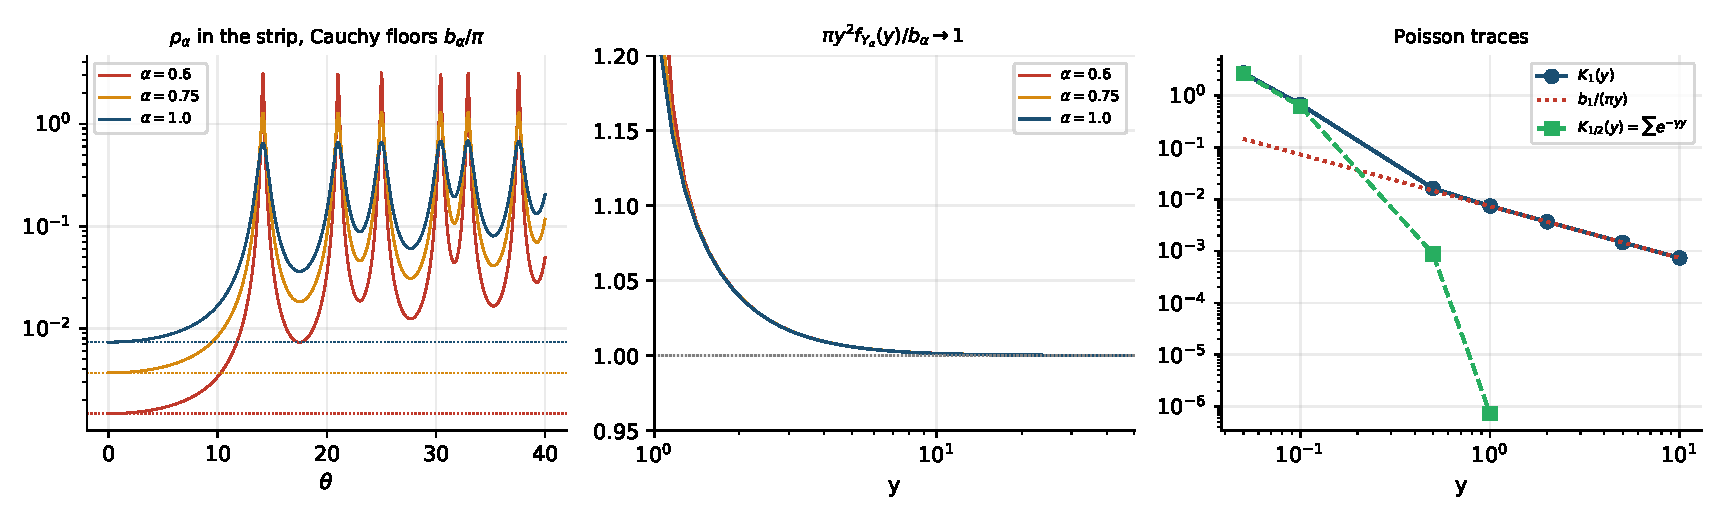
\includegraphics[width=\textwidth]{fig/bp1_strip.pdf}
\caption{Left: the Thorin densities $v_\alpha/\pi$ at $\alpha=0.6$, $0.75$, $1$, written $\rho_\alpha$ in the plot, and their Cauchy floors $b_\alpha/\pi$ (dotted). Middle: $\pi y^2f_{Y_\alpha}(y)/b_\alpha$, tending to one. Right: the Poisson traces $K_1$ and $K_{1/2}$ against $b_1/(\pi y)$. Drawn by \texttt{figs2.py} from \texttt{strip.json} and \texttt{comp.json}.}
\label{sm:fig:strip}
\end{figure}

Frullani's integral gives $\log(1+u^2/\theta^2)=\int_{\R}(1-\cos uy)\,e^{-\theta|y|}\frac{dy}{|y|}$, which is the sine squared lemma read in the other direction, since $1-\cos uy=2\sin^2(uy/2)$, and which is the cosine dictionary \eqref{rz:eq:cosdict} of Section~\ref{ch:rz2}. Inserting it in \eqref{sm:eq:thorin} puts the characteristic function of $Y_\alpha$ in L\'evy Khintchine form in $u$:
\begin{gather*}
\frac{\xi(\alpha)}{\xi(\alpha+|u|)}=\exp\Big\{-\int_{\R}2\sin^2\Big(\frac{uy}2\Big)\,\frac{K_\alpha(|y|)}{|y|}\,dy\Big\},\\
K_\alpha(y)=\frac1\pi\int_0^\infty e^{-\theta y}v_\alpha(\theta)\,d\theta .
\end{gather*}
So the L\'evy density of $Y_\alpha$ is $K_\alpha(|y|)/|y|$, as Section~\ref{sec:ch3:hierarchy} gives for a symmetric EGGC, and $K_\alpha$ is the Laplace transform of the Thorin density; in the normalisation of \eqref{rz:eq:cosdict}, $K_\alpha=\frac12K_{U_\alpha}$. We call $K_\alpha$ the Poisson trace, because at the centre, where under RH the Thorin measure in the chart $\theta$ is $\sum_{\gamma>0}\delta_\gamma$, it is $K_{1/2}(y)=\sum_{\gamma>0}e^{-\gamma y}$, half of Cram\'er's function \cite[Chapter I]{Cramer19} of Proposition~\ref{rz:prop:dict}(iii): the sum over the zeros of the Poisson kernel in place of the heat kernel of the heat trace $W(t)=\sum_ke^{-a_kt}$, which is $\sum_{\gamma>0}e^{-\gamma^2t}$ under RH. The two traces play parallel roles, and they are linked with no hypothesis. Since $Y_{1/2}=B_{2T}$ for an independent Brownian motion $B$, and $T$ has L\'evy density $W(t)/t$ (Theorem~\ref{thm:ch12:idsd}), the L\'evy density of $Y_{1/2}$ is $\int_0^\infty(4\pi t)^{-1/2}e^{-y^2/4t}\,W(t)\,t^{-1}dt$, so
\[
K_{1/2}(y)=\int_0^\infty\frac{y}{\sqrt{4\pi t^3}}\,e^{-y^2/4t}\,W(t)\,dt=\E\,W(H_{y/\sqrt2}),\qquad y>0 .
\]
The Poisson trace is the heat trace averaged over the first passage time of Brownian motion to the level $y/\sqrt2$, that is, subordinated by the stable one half first passage kernel, whose Laplace transform $e^{-y\sqrt a}$ is the stable one half average of the heat kernel recalled after Proposition~\ref{rz:prop:diverge}. This defines $K_{1/2}$ unconditionally, as $K_{1/2}(y)=\sum_ke^{-y\sqrt{a_k}}$ with the principal root, and makes it computable from the explicit formula \eqref{eq:ch2:Warith} for $W$; under RH the kernel integrates $e^{-\gamma^2t}$ to $e^{-\gamma y}$. Numerically, \texttt{improve.py} evaluates the integral with $W$ from the first $1700$ zeros and obtains $0.08566744234217$ at $y=0.2$ and $0.000883746148510$ at $y=0.5$, equal to $\sum e^{-\gamma y}$ over the same zeros to fourteen digits.

\begin{corollary}\label{sm:cor:poisson}
RH holds if and only if the Poisson trace $K_{1/2}$ is completely monotone, and if and only if the heat trace $W$ is completely monotone. For $\alpha\ge1$ the Poisson trace $K_\alpha$ is completely monotone with no hypothesis, and $K_\alpha(y)\sim b_\alpha/(\pi y)$ as $y\to\infty$, so that the L\'evy density of $Y_\alpha$ is asymptotic to $b_\alpha/(\pi y^2)$, the L\'evy density of the Cauchy component.
\end{corollary}

\begin{proof}
For $\alpha\ge1$, $K_\alpha$ is the Laplace transform of the positive density $v_\alpha/\pi$, hence completely monotone by Bernstein's theorem, and since $v_\alpha$ is continuous with $v_\alpha(0)=b_\alpha$, $yK_\alpha(y)\to b_\alpha/\pi$ as $y\to\infty$. At the centre, $W$ is completely monotone exactly when $T$ is a GGC (Section~\ref{ch:clock}), that is exactly when RH holds (Proposition~\ref{prop:rigid}). Under RH, $K_{1/2}(y)=\sum_{\gamma>0}e^{-\gamma y}$ is completely monotone. Conversely, suppose that $K_{1/2}(y)=\int_{[0,\infty)}e^{-y\theta}\nu(d\theta)$ with a positive measure $\nu$. For $w>0$ the unconditional formula $K_{1/2}(y)=\sum_ke^{-y\sqrt{a_k}}$ gives
\[
\int_0^\infty e^{-wy}\,y\,K_{1/2}(y)\,dy=\sum_k\frac1{(w+\sqrt{a_k})^2}=\int_{[0,\infty)}\frac{\nu(d\theta)}{(w+\theta)^2}.
\]
The first equality integrates term by term, which is legitimate because $\sqrt{a_k}=\gamma_k-i(\beta_k-\frac12)$ has real part $\gamma_k$ when $\rho_k=\beta_k+i\gamma_k$ is taken with $\gamma_k>0$, so the absolute values of the terms integrate to $\sum_k(w+\gamma_k)^{-2}<\infty$. The second is Tonelli's theorem, and it shows that the right side is finite for $w>0$. The middle expression is meromorphic in $w\in\C$, with a double pole at each point $-\sqrt{a_k}$, while the right side is holomorphic on $\cut$, since $|w+\theta|$ is bounded below by a positive multiple of $1+\theta$ for $w$ in a compact subset of $\cut$. The two sides agree for $w>0$, hence on $\cut$ with the poles removed, so no pole $-\sqrt{a_k}$ lies in $\cut$. Since $\re\sqrt{a_k}>0$, every $\sqrt{a_k}$ is therefore real and positive, that is, every $a_k=-(\rho_k-\frac12)^2$ is positive, which is RH.
\end{proof}

Table~\ref{sm:tab:K}, computed by \texttt{comp.py}, gives $K_1$ from $v_1$ on $[0,200]$ with the Weyl density beyond, and $K_{1/2}$ as $\sum e^{-\gamma y}$ over the first $1700$ zeros (Figure~\ref{sm:fig:strip}, right). At large $y$, $K_1(y)$ approaches $b_1/(\pi y)$, to $0.5\%$ at $y=10$, while $K_{1/2}(y)$ decays like $e^{-\gamma_1y}$: at the centre there is no Cauchy component, the tail is Laplace like with rate $\gamma_1$, and the variance is finite. At small $y$ both traces are large and close, because there the Poisson kernels see all zeros and the smoothing at the basepoint one matters little.

\begin{table}[htbp]
\centering\small
\begin{tabular}{cccc}
\toprule
$y$ & $K_1(y)=\frac1\pi\int_0^\infty e^{-\theta y}v_1(\theta)\,d\theta$ & $b_1/(\pi y)$ & $K_{1/2}(y)=\sum e^{-\gamma y}$\\
\midrule
0.05 & 2.7700 & 0.1470 & 2.6860\\
0.1 & 0.68408 & 0.07352 & 0.62104\\
0.5 & 0.016327 & 0.014703 & $8.84\times10^{-4}$\\
1 & 0.0074306 & 0.0073516 & $7.27\times10^{-7}$\\
2 & 0.0036856 & 0.0036758 & $5.28\times10^{-13}$\\
10 & 0.00073906 & 0.00073516 & $4.1\times10^{-62}$\\
\bottomrule
\end{tabular}
\caption{The Poisson traces at the basepoint one and at the centre, computed by \texttt{comp.py}.}
\label{sm:tab:K}
\end{table}

\subsection{The complete monotonicity conditions of the Poisson trace}\label{sec:biane:cm}

By Corollary~\ref{sm:cor:poisson}, RH is the complete monotonicity of the Poisson trace $K_{1/2}$. This subsection follows the first author's note on Biane's paper \cite{P26bia}. It writes the conditions out zero by zero, proves that a long initial stretch of them holds with no hypothesis, says which zeros each condition sees, gives two further equivalent forms, explains why the explicit formula cannot test the conditions, and compares $K_{1/2}$ with the corresponding trace of P\'olya's function $P(\theta)=K_{i\theta/2}(2\pi)$ of Section~\ref{ch:biane}, which is completely monotone with no hypothesis. The computations are in \texttt{biane\_traces.py} and \texttt{biane\_figs.py}.

Write the zeros as $\rho_k=\beta_k+i\gamma_k$ with $\gamma_k>0$, so that $\sqrt{a_k}=\gamma_k+i\delta_k$ with $\delta_k=\frac12-\beta_k\in(-\frac12,\frac12)$, and put $\varphi_k=\arctan(\delta_k/\gamma_k)$. The series $K_{1/2}(y)=\sum_ke^{-y\sqrt{a_k}}$ converges absolutely, with all its derivatives, for $y>0$, and the zeros $\rho_k$ and $1-\bar\rho_k$ have conjugate values of $\sqrt{a_k}$. Hence
\begin{equation}\label{eq:biane:cmcond}
(-1)^nK_{1/2}^{(n)}(y)=\sum_k\re\big((\sqrt{a_k})^ne^{-y\sqrt{a_k}}\big)=\sum_k|\sqrt{a_k}|^n\,e^{-\gamma_ky}\cos(n\varphi_k-\delta_ky),
\end{equation}
with each zero counted once, with its multiplicity; a zero on the line contributes $\gamma_k^ne^{-\gamma_ky}>0$. The note \cite{P26bia} groups $\rho_k$ with $1-\bar\rho_k$ and writes a factor $2$ in front of every term, which counts the zeros on the line twice. So $K_{1/2}$ is completely monotone, and by Corollary~\ref{sm:cor:poisson} RH holds, exactly when every one of the quantities \eqref{eq:biane:cmcond} is nonnegative, for $n=0,1,2,\dots$ and $y>0$. Off the line a term oscillates in $n$ with the small frequency $\varphi_k\approx\delta_k/\gamma_k$, so a zero off the line can spoil its term only at a high order.

\begin{proposition}\label{prop:biane:termwise}
The term of a zero with $\delta_k\ne0$ in \eqref{eq:biane:cmcond} is positive whenever
\[
n\arctan\frac{|\delta_k|}{\gamma_k}+|\delta_k|\,y<\frac\pi2 .
\]
If $\delta_k>0$ and $\delta_ky<\frac\pi2$, the first order $n$ at which the term is negative is the least integer with $n\varphi_k-\delta_ky>\frac\pi2$, that is the least integer above $(\frac\pi2+\delta_ky)/\varphi_k$ when this ratio is not an integer. The partner $1-\bar\rho_k$ has the same term.
\end{proposition}

\begin{proof}
$|n\varphi_k-\delta_ky|\le n|\varphi_k|+|\delta_k|y$, and the cosine is positive on $(-\frac\pi2,\frac\pi2)$. For $\delta_k>0$ the argument $n\varphi_k-\delta_ky$ increases with $n$ from $-\delta_ky\in(-\frac\pi2,0)$, and the cosine is first negative when it passes $\frac\pi2$. The partner has $-\delta_k$ and $-\varphi_k$, so its argument is the negative of this one.
\end{proof}

\texttt{biane\_traces.py} finds the first negative order by evaluating the sign factor; Table~\ref{tab:biane:cmorders} compares it with the formula, and the note's values are the same.

\begin{table}[htbp]
\centering\small
\begin{tabular}{rrrrr}
\toprule
$\gamma$ & $\delta$ & $y$ & first negative order & $(\frac\pi2+\delta y)/\varphi$\\
\midrule
$50$ & $0.25$ & $1$ & $365$ & $364.16$\\
$50$ & $0.25$ & $0.3$ & $330$ & $329.16$\\
$200$ & $0.1$ & $1$ & $3342$ & $3341.59$\\
$14.13$ & $0.5$ & $0.5$ & $52$ & $51.48$\\
\bottomrule
\end{tabular}
\caption{The first order at which the term of a hypothetical zero $\frac12-\delta+i\gamma$ in \eqref{eq:biane:cmcond} is negative, against Proposition~\ref{prop:biane:termwise}. The last row is a zero at the edge of the strip at the height of the first ordinate. Computed by \texttt{biane\_traces.py}.}
\label{tab:biane:cmorders}
\end{table}

\begin{theorem}\label{thm:biane:cmrange}
Suppose that every zero with $0<\gamma_k\le H$ lies on the critical line. Then for $0<y<\pi$ and every integer $n$ with $0\le n<H(\pi-y)$, every term of \eqref{eq:biane:cmcond} is positive, and $(-1)^nK_{1/2}^{(n)}(y)>0$. With $H=T_0=3\times10^{12}$ \cite{PT21} this covers all $n<9.12\times10^{12}$ at $y=0.1$, $n<6.42\times10^{12}$ at $y=1$ and $n<4.24\times10^{11}$ at $y=3$.
\end{theorem}

\begin{proof}
A zero with $\gamma_k\le H$ has $\delta_k=0$, and its term $\gamma_k^ne^{-\gamma_ky}$ is positive. A zero with $\gamma_k>H$ has $|\varphi_k|\le|\delta_k|/\gamma_k<\frac1{2H}$ and $|\delta_k|y<\frac y2$, so $n|\varphi_k|+|\delta_k|y<\frac n{2H}+\frac y2\le\frac\pi2$ when $n\le H(\pi-y)$, and its term is positive by Proposition~\ref{prop:biane:termwise}. The series converges absolutely, so its sum is positive.
\end{proof}

The theorem is a statement about the verified height, not about $K_{1/2}$: it improves with every extension of the verification and never reaches the whole family. Every condition that could fail has $y\ge\pi$ or $n\ge H(\pi-y)$, which is above $4\times10^{11}$ for $y\le3$; there, complete monotonicity is a characterisation of RH, not a test that a computation could run to a failure. The note \cite{P26bia} gives the last bound as $4.3\times10^{11}$; it is $4.2478\times10^{11}$.

The weight of the zero $\gamma_k$ in the condition $(n,y)$ is about $\gamma_k^ne^{-\gamma_ky}$, whose logarithm $n\log\gamma-\gamma y$ is largest at
\[
\gamma_*=\frac ny,
\]
with a width of order $\sqrt n/y$. The condition $(n,y)$ is therefore a smoothed probe of the zeros near the height $n/y$. Among the first $300$ ordinates the dominant one is $21.022$ for $(n,y)=(20,1)$, $98.831$ for $(100,1)$ and for $(50,0.5)$, with $101.318$ a close second (the logarithms of the weights at $(100,1)$ are $360.51013$ and $360.50841$), $21.022$ for $(100,5)$ and $30.425$ for $(300,10)$: in each case the ordinate nearest to $n/y$ (\texttt{biane\_traces.py}). Figure~\ref{fig:biane:cm} shows two weight profiles and two sign factors. The reading explains Theorem~\ref{thm:biane:cmrange} and shows its edge. By Proposition~\ref{prop:biane:termwise} a zero at height $\gamma$ can make its term negative only when $n\gtrsim\frac\pi2\gamma/|\delta|\ge\pi\gamma$, that is when $\gamma\lesssim n/\pi$, below the peak at $n/y$ when $y<\pi$; and since $\gamma^ne^{-\gamma y}$ increases up to $n/y$, its value at $\gamma\le n/\pi$ is at most $\exp(n(\log\frac y\pi+1-\frac y\pi))$ times its value at the peak, which is exponentially small in $n$. Turning this comparison into a proof would need a bound for the number of zeros off the line near each height, and it would push the unconditional range beyond $H(\pi-y)$ without reaching the whole family: the conditions with $n/y$ beyond every verified height are the content of RH.

\begin{figure}[htbp]
\centering
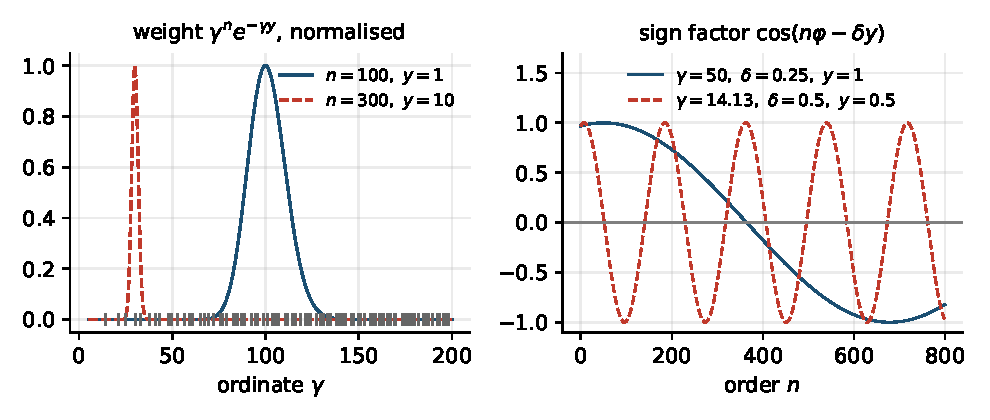
\includegraphics[width=\textwidth]{fig/biane_cm.pdf}
\caption{Left: the weight $\gamma^ne^{-\gamma y}$ of the condition $(n,y)$ in \eqref{eq:biane:cmcond}, normalised to maximum one, for $(n,y)=(100,1)$ and $(300,10)$, peaking at $\gamma=n/y$; the marks are the ordinates below $200$. Right: the sign factor $\cos(n\varphi-\delta y)$ of a hypothetical zero off the line for $(\gamma,\delta,y)=(50,0.25,1)$ and $(14.13,0.5,0.5)$, positive below the orders $365$ and $52$ of Table~\ref{tab:biane:cmorders}, at which it is first negative. Drawn by \texttt{biane\_figs.py} from \texttt{biane\_traces.json}.}
\label{fig:biane:cm}
\end{figure}

\begin{proposition}\label{prop:biane:pd}
The following are equivalent:
\begin{enumerate}
\item[(i)] RH;
\item[(ii)] $K_{1/2}$ is completely monotone on $(0,\infty)$;
\item[(iii)] for every $x>0$ the function $y\mapsto K_{1/2}(x+iy)$ is positive definite on $\R$;
\item[(iv)] for some $x>0$ the function $y\mapsto K_{1/2}(x+iy)$ is bounded on $[0,\infty)$.
\end{enumerate}
Under these conditions $|K_{1/2}(x+iy)|\le K_{1/2}(x)$.
\end{proposition}

\begin{proof}
The series $K_{1/2}(z)=\sum_ke^{-z\sqrt{a_k}}$ converges absolutely and locally uniformly for $\re z>0$, since $|e^{-z\sqrt{a_k}}|=e^{-\gamma_k\re z+\delta_k\im z}\le e^{-\gamma_k\re z+|\im z|/2}$, and defines an analytic function there. (i) implies (ii) by Corollary~\ref{sm:cor:poisson}. If (ii) holds, Bernstein's theorem gives $K_{1/2}(y)=\int_{[0,\infty)}e^{-y\theta}\nu(d\theta)$ with a positive measure $\nu$, the integral converges for $\re z>0$ and agrees there with $K_{1/2}(z)$ by analytic continuation, and $K_{1/2}(x+iy)=\int e^{-iy\theta}e^{-x\theta}\nu(d\theta)$ is the Fourier transform of the finite positive measure $e^{-x\theta}\nu(d\theta)$, which gives (iii) and the bound. A positive definite function $f$ satisfies $|f(y)|\le f(0)$, so (iii) implies (iv). Suppose (iv) holds at $x$. For $\re w>\frac12$ the bound above allows term by term integration, and
\[
\int_0^\infty e^{-wy}K_{1/2}(x+iy)\,dy=\sum_k\frac{e^{-x\sqrt{a_k}}}{w+i\sqrt{a_k}} .
\]
The right side is a meromorphic function of $w\in\C$, since $\sum_ke^{-x\gamma_k}<\infty$, with a pole at each point $-i\sqrt{a_k}=\delta_k-i\gamma_k$, of residue $e^{-x\sqrt{a_k}}$ times the multiplicity, which is not zero. Since $K_{1/2}(x+iy)$ is bounded, the left side is analytic in $\re w>0$, so no pole has $\delta_k>0$. The zeros $\rho_k$ and $1-\bar\rho_k$ have opposite $\delta_k$, so every $\delta_k$ is $0$, which is RH.
\end{proof}

Part (iv) replaces the Paley Wiener argument of the note \cite{P26bia}, which is not given in detail there, by a pole of a Laplace transform. Written out, (iii) says that for every $x>0$, all real $y_1,\dots,y_m$ and all complex $c_1,\dots,c_m$,
\[
\sum_{j,l}c_j\bar c_l\,K_{1/2}\big(x+i(y_j-y_l)\big)=\sum_ke^{-x\gamma_k}\Big|\sum_jc_je^{-i\gamma_ky_j}\Big|^2\ge0,
\]
the equality holding under RH. This is a positivity of the kind in Weil's criterion, with two differences: the test functions are $r\mapsto e^{-rx}|\sum_jc_je^{-iry_j}|^2$ on $r>0$, where the damping $e^{-rx}$ does the work of a decay hypothesis, and the sum runs over the ordinates in the upper half plane only.

One would like to turn each condition into a statement about primes with the explicit formula of Section~\ref{ch:clock}, the display before \eqref{eq:ch2:Warith}. The test function of the condition $(n,y)$ is $h(r)=|r|^ne^{-y|r|}$, with
\[
g(x)=\frac1{2\pi}\int_{\R}h(r)e^{-irx}\,dr=\frac{n!}\pi\re\frac1{(y+ix)^{n+1}},
\]
which decays only like a power of $|x|$ and has one sign for large $|x|$. The prime side $-2\sum_{m\ge2}\Lambda(m)m^{-1/2}g(\log m)$ then diverges, since $\sum_pp^{-1/2}(\log p)^{-j}=\infty$ for every $j$; the formula holds for $g$ decaying faster than $e^{-|x|/2}$, which goes with $h$ analytic in a strip $|\im r|<\frac12+\epsilon$, and this $h$ is not even analytic at $r=0$. For $n=0$ the prime side is $-\frac2\pi\sum_{m\ge2}\Lambda(m)m^{-1/2}y/(y^2+\log^2m)$, which is what the prime terms of \eqref{eq:ch2:Warith} become under the subordination $K_{1/2}(y)=\E W(H_{y/\sqrt2})$ of Section~\ref{sm:sec:poisson}, applied term by term, with twice $K_{1/2}$ on the left; its terms have poles at $y=\pm i\log m$, the singularities of Cram\'er's function \cite[Chapter I]{Cramer19}, and it diverges for the reason of Proposition~\ref{rz:prop:diverge}. Smoothing in the variable of the zeros removes the divergence without changing the problem: the Gaussian weight $e^{-r^2t}$ in place of $e^{-y|r|}$ gives the heat trace $W(t)$, whose explicit formula \eqref{eq:ch2:Warith} converges absolutely, and whose complete monotonicity is again equivalent to RH (Corollary~\ref{sm:cor:poisson}). The note \cite{P26bia} identifies this smoothing with the de Bruijn Newman flow and concludes that the primes become summable only at times $t>0$, where the reality of the zeros is known; but the Gaussian weight acts on the test function, while the flow multiplies the kernel $\Phi$ by $e^{tu^2/4}$ and moves the zeros, and the smoothed conditions, those of the heat trace, are still equivalent to RH.

The last comparison is with P\'olya's function. By Proposition~\ref{prop:biane:sin2},
\begin{gather*}
\log\frac{K_{\lambda/2}(2\pi)}{K_0(2\pi)}=\int_0^\infty4\sin^2\Big(\frac{\lambda y}2\Big)K^P(y)\,\frac{dy}y,\\
K^P(y)=\sum_ne^{-2\nu_ny}=\operatorname{tr}e^{-2y\sqrt{A_P}},
\end{gather*}
the sum over the zeros $\theta_n=2\nu_n$ of $P$, so $K^P$ is the counterpart of $K_{1/2}$ in the formula for $\xi(\frac12)/\xi(\frac12+u)$, and it is completely monotone because $A_P$ is selfadjoint and positive. By Proposition~\ref{prop:biane:phase} the two traces have the same main term, and their difference has a limit.

\begin{proposition}\label{prop:biane:traces}
Let $M(y)=\frac1{2\pi y}\big(\log\frac1{2\pi y}-\gamma_E\big)$ and $c=2\pi-\frac1{6\pi}-\frac1{48\pi}=6.2235022035$. As $y\to0+$:
\begin{enumerate}
\item[(i)] $K_{1/2}(y)=M(y)+\frac78+O(y\log\frac1y)$, and under RH $K_{1/2}(y)=M(y)+\frac78+\frac1{48\pi}y\log\frac1y+o(y\log\frac1y)$;
\item[(ii)] $K^P(y)=M(y)-\frac14+\big(2\pi-\frac1{6\pi}\big)y\log\frac1y+O(y)$;
\item[(iii)] $D(y)=K_{1/2}(y)-K^P(y)=\frac98+O(y\log\frac1y)$, and under RH $D(y)=\frac98-c\,y\log\frac1y+o(y\log\frac1y)$.
\end{enumerate}
\end{proposition}

\begin{proof}
(i) The real part of the term $e^{-y\sqrt{a_k}}$ is $e^{-\gamma_ky}\cos(\delta_ky)=e^{-\gamma_ky}+O(y^2e^{-\gamma_ky})$, and the imaginary parts cancel in pairs, so $K_{1/2}(y)=\sum_ke^{-\gamma_ky}+O(y^2\sum_ke^{-\gamma_ky})$, and the sum will turn out to be $O(y^{-1}\log\frac1y)$. By Abel summation $\sum_ke^{-\gamma_ky}=y\int_0^\infty e^{-Ty}N(T)\,dT$, with $N(T)=\vartheta(T)/\pi+1+S(T)$ \cite[Section 9.3]{Titchmarsh}. The Riemann Siegel function satisfies $\vartheta(T)/\pi=N_0(T)-\frac18+\frac1{48\pi T}+O(T^{-3})$ with $N_0(T)=\frac T{2\pi}\log\frac T{2\pi e}$, so $N=N_0+\frac78+S+E$ with $E(T)=\frac1{48\pi T}+O(T^{-3})$ for $T\ge1$ and $E$ bounded on $(0,1]$. Now $\int_0^\infty Te^{-Ty}\log T\,dT=y^{-2}(1-\gamma_E-\log y)$ gives $y\int_0^\infty e^{-Ty}N_0(T)\,dT=M(y)$; the constant gives $\frac78$; $y\int_1^\infty e^{-Ty}\frac{dT}{48\pi T}=\frac1{48\pi}y\log\frac1y+O(y)$, and the rest of $E$ gives $O(y)$. With $S_1(T)=\int_0^TS(t)\,dt$, an integration by parts gives $y\int_0^\infty e^{-Ty}S(T)\,dT=y^2\int_0^\infty e^{-Ty}S_1(T)\,dT$, which is $O(y\log\frac1y)$ since $S_1(T)=O(\log T)$ \cite[Theorem 9.9(A)]{Titchmarsh}. Under RH there are no terms $O(y^2e^{-\gamma_ky})$, and $S_1(T)=O(\log T/(\log\log T)^2)$ \cite[Theorem 14.13]{Titchmarsh} makes the last integral $o(y\log\frac1y)$. (ii) By Proposition~\ref{prop:biane:phase}, the number of zeros $\theta_n\le T$ is $\lfloor x(T)\rfloor$, with $x(T)=N_0(T)+\frac14+(2\pi-\frac1{6\pi})T^{-1}+O(T^{-3})$ for $T\ge1$. Write $\lfloor x\rfloor=x-\frac12+(\frac12-\{x\})$. The terms $N_0$, $\frac14-\frac12$ and $(2\pi-\frac1{6\pi})T^{-1}$ give $M(y)$, $-\frac14$ and $(2\pi-\frac1{6\pi})y\log\frac1y+O(y)$ as in (i). The sawtooth $\frac12-\{x(T)\}$ has integral over each interval on which $x$ increases by one equal to $O(T^{-1}(\log T)^{-3})$, because such an interval has length about $2\pi/\log T$ and $x'(T)=\frac1{2\pi}\log\frac T{2\pi}+O(T^{-2})$ varies over it by $O(T^{-1}(\log T)^{-2})$ relative to its size, so its integral from $0$ to $T$ is bounded, and another integration by parts makes its contribution $O(y)$. (iii) is (i) minus (ii).
\end{proof}

\texttt{biane\_traces.py} tests the proposition. It takes the first $30000$ ordinates from Arb, up to $25755.348$, cuts at $G=25754.905$, midway between the last two, and adds the tail $\int_G^\infty e^{-Ty}\vartheta'(T)\,dT/\pi-e^{-Gy}S(G)$, with $S(G)=-0.569$ exact; the neglected term $y\int_G^\infty e^{-Ty}S(T)\,dT$ equals $y^2\int_G^\infty e^{-Ty}\int_G^TS(t)\,dt\,dT$, and Trudgian's bound $|\int_{t_1}^{t_2}S(t)\,dt|\le2.067+0.059\log t_2$ for $t_2>t_1>168\pi$ \cite{Trudgian11}, with Jensen's inequality for the logarithm, bounds it by $ye^{-Gy}(0.059\log(G+1/y)+2.067)$; the script records twice this bound, $3.5\times10^{-14}$, $4.1\times10^{-5}$ and $4.3\times10^{-5}$ at $y=10^{-3}$, $10^{-4}$ and $10^{-5}$, so the entries of Table~\ref{tab:biane:traces} at $y=10^{-4}$ and $10^{-5}$ may be off by up to two units in the fifth decimal. The zeros of $P$ come from the phase condition of Proposition~\ref{prop:biane:phase}, solved by Newton's method for all $30132$ zeros to just above the cut, with phase residuals below $4.4\times10^{-11}$; the $29998$ below $G$ are summed and the tail $\int_G^\infty e^{-Ty}\,dx(T)+e^{-Gy}(\{x(G)\}-\frac12)$ is added, with $x(G)=29998.944$. The factor $e^{-Gy}$ that weights the tails is $2.6\times10^{-6}$ at $y=5\times10^{-4}$, $0.0058$ at $2\times10^{-4}$, $0.076$ at $10^{-4}$ and $0.77$ at $10^{-5}$, so the last row of Table~\ref{tab:biane:traces} rests mostly on the smooth tails. The constant $\frac98$ appears clearly, and $D$ approaches it along $\frac98-cy\log\frac1y$ (Figure~\ref{fig:biane:traces}).

\begin{table}[htbp]
\centering\small
\fitwidth{\begin{tabular}{lrrrrrr}
\toprule
$y$ & $K_{1/2}(y)$ & $K^P(y)$ & $K_{1/2}-M$ & $K^P-M$ & $D(y)$ & $\frac98-cy\log\frac1y$\\
\midrule
$0.05$ & $2.686015$ & $2.230883$ & $0.837782$ & $0.382650$ & $0.455132$ & $0.192803$\\
$0.02$ & $12.772471$ & $12.033884$ & $0.860279$ & $0.121691$ & $0.738587$ & $0.638070$\\
$0.01$ & $35.723862$ & $34.836495$ & $0.867696$ & $-0.019670$ & $0.887366$ & $0.838397$\\
$0.005$ & $92.647265$ & $91.663043$ & $0.871374$ & $-0.112848$ & $0.984222$ & $0.960130$\\
$0.003$ & $180.932794$ & $179.901902$ & $0.872836$ & $-0.158057$ & $1.030892$ & $1.016540$\\
$0.002$ & $303.229389$ & $302.172210$ & $0.873563$ & $-0.183616$ & $1.057179$ & $1.047647$\\
$0.001$ & $715.903738$ & $714.816981$ & $0.874286$ & $-0.212471$ & $1.086757$ & $1.082010$\\
$5\times10^{-4}$ & $1651.569150$ & $1650.465433$ & $0.874645$ & $-0.229071$ & $1.103717$ & $1.101348$\\
$2\times10^{-4}$ & $4856.772117$ & $4855.656772$ & $0.874859$ & $-0.240486$ & $1.115345$ & $1.114399$\\
$10^{-4}$ & $10815.847446$ & $10814.727704$ & $0.874931$ & $-0.244811$ & $1.119742$ & $1.119268$\\
$10^{-5}$ & $144797.380092$ & $144796.255761$ & $0.874994$ & $-0.249338$ & $1.124332$ & $1.124283$\\
\bottomrule
\end{tabular}}
\caption{The Poisson trace $K_{1/2}$ of the zeros of $\zeta$, P\'olya's trace $K^P$, their distances from the common main term $M$, which tend to $\frac78$ and $-\frac14$, and their difference $D$, which tends to $\frac98$, against the prediction of Proposition~\ref{prop:biane:traces} under RH. Computed by \texttt{biane\_traces.py}.}
\label{tab:biane:traces}
\end{table}

\begin{figure}[htbp]
\centering
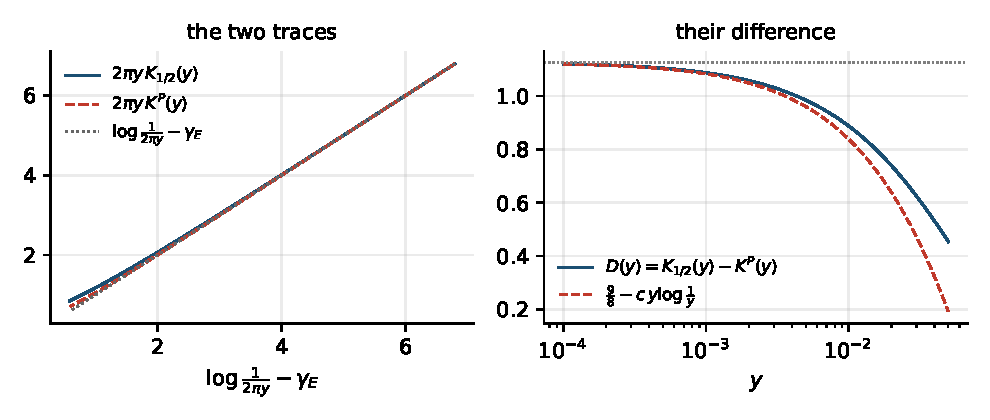
\includegraphics[width=\textwidth]{fig/biane_traces.pdf}
\caption{Left: $2\pi yK_{1/2}(y)$ and $2\pi yK^P(y)$ against $\log\frac1{2\pi y}-\gamma_E$ for $10^{-4}\le y\le0.05$, with the main term $2\pi yM(y)$ (dotted). Right: the difference $D(y)$, the limit $\frac98$ (dotted) and $\frac98-cy\log\frac1y$ (dashed). Drawn by \texttt{biane\_figs.py} from \texttt{biane\_traces.json}.}
\label{fig:biane:traces}
\end{figure}

The note \cite{P26bia} states that $K_{1/2}(y)=M(y)+O(\log\frac1y)$, which is true but loses the constant, and it reports $D(y)/\log\frac1y=0.195$, $0.194$, $0.193$, $0.193$ at $y=0.003$, $0.005$, $0.01$, $0.02$, from which it concludes that $D$ grows like $0.19\log\frac1y$. Repeating its computation, with the first $300$ ordinates and the $312$ zeros of $P$ below $\gamma_{300}+20=561.85$, each followed by a plain Weyl tail from the last zero, gives its ratios $K_{1/2}/M=1.0059$, $1.0102$, $1.0250$, $1.0722$ and $D/\log\frac1y=0.195$, $0.192$, $0.193$, $0.189$; the note describes the $312$ zeros as lying below $\gamma_{300}=541.85$, below which there are $298$. The accurate values of $D/\log\frac1y$ in this range, $0.177$, $0.186$, $0.193$, $0.189$, are also close to $0.19$, but that is a coincidence of the range: by Proposition~\ref{prop:biane:traces}, $D$ tends to $\frac98$, and $D/\log\frac1y$ is $0.098$ at $y=10^{-5}$.

The comparison shows where the difficulty sits. $K^P$ is completely monotone for a structural reason, as the trace of the semigroup $e^{-2y\sqrt{A_P}}$. By Corollary~\ref{sm:cor:poisson}, RH says that $K_{1/2}=K^P+D$ is completely monotone as well, where $D$ is bounded, tends to $\frac98$ while both traces grow like $\frac1{2\pi y}\log\frac1y$, and carries the whole difference between $\Phi$ and P\'olya's kernel, the arithmetic included. Complete monotonicity constrains the derivatives of every order, and no bound on the size of $D$ can decide it.

\subsection{Wiener's theorem and the basepoint kernels}\label{wr:sec:wiener}

The zero free half planes that recur through Chapter~\ref{chap:basepoint} and through Sections~\ref{sm:sec:cf} to \ref{sm:sec:poisson} have a second reading, as completeness statements, through Wiener's closure theorem \cite{Wiener32}, for which Kac \cite{Kac65} and Korevaar \cite{Korevaar65} gave short alternative treatments: the translates $f(\cdot-x)$, $x\in\R$, of a function $f\in L^1(\R)$ span a dense subspace of $L^1(\R)$ if and only if its Fourier transform $\hat f(\theta)=\int f(u)e^{i\theta u}du$ has no real zeros. The $L^2$ version asks only that $\hat f\ne0$ almost everywhere; since the zeros of $\xi$ are isolated it never sees them, and it is the $L^1$ version that is sharp here.

Let $\Phi$ be P\'olya's kernel \eqref{eq:ch2:Phi}, so that $\xi(\frac12+s)=\int_{\R}\Phi(u)e^{su}du$ for every complex $s$ by \eqref{eq:ch2:mgf}, and for $\alpha\ge\frac12$ put
\begin{equation}\label{wr:eq:kernel}
\Phi_\alpha(u)=e^{(\alpha-\frac12)u}\,\Phi(u),\qquad \hat\Phi_\alpha(\theta)=\int_{\R}\Phi_\alpha(u)e^{i\theta u}du=\xi(\alpha+i\theta).
\end{equation}
Up to the factor $\xi(\alpha)$, $\Phi_\alpha$ is the density of the tilted P\'olya variable $V_\alpha$ of Section~\ref{bp:sec:mellin}, with $\E e^{sV_\alpha}=\xi(\alpha+s)/\xi(\alpha)$, and it is integrable for every $\alpha$ because $\Phi$ decays doubly exponentially. The real zeros of $\hat\Phi_\alpha$ are exactly the ordinates of the zeros of $\zeta$ on the line $\re s=\alpha$, so Wiener's theorem gives the following.

\begin{proposition}\label{wr:prop:wiener}
\begin{enumerate}
\item The translates of $\Phi_\alpha$ are dense in $L^1(\R)$ if and only if $\zeta$ has no zeros on the line $\re s=\alpha$.
\item At the centre they are not dense. For every finite combination $h=\sum_kc_k\Phi(\cdot-x_k)$ and every $g\in L^1(\R)$,
\[
\|g-h\|_1\ \ge\ \sup_\gamma|\hat g(\gamma)|,
\]
the supremum over the ordinates of the zeros on the critical line.
\item At the basepoint one they are dense, with no hypothesis, because $\xi(1+i\theta)\ne0$.
\item For $\alpha_0\in[\frac12,1)$, $\zeta$ has no zeros in the half plane $\re s>\alpha_0$ if and only if the translates of $\Phi_\alpha$ are dense in $L^1(\R)$ for every $\alpha>\alpha_0$. In particular RH holds if and only if they are dense for every $\alpha>\frac12$.
\item If the translates of $\Phi_\alpha$ are dense, approximation near the zeros is expensive: if $h=\sum_kc_k\Phi_\alpha(\cdot-x_k)$ and $\|g-h\|_1\le\delta$, then $\sum_k|c_k|\ \ge\ (|\hat g(\gamma)|-\delta)/|\xi(\alpha+i\gamma)|$ for every ordinate $\gamma$.
\end{enumerate}
\end{proposition}

\begin{proof}
(1), (3) and (4) are Wiener's theorem applied to $\hat\Phi_\alpha(\theta)=\xi(\alpha+i\theta)$, together with the nonvanishing of $\zeta$ on the line $\re s=1$. For (2) and (5), $\hat h(\theta)=\hat\Phi_\alpha(\theta)\sum_kc_ke^{i\theta x_k}$, so at the centre $\hat h(\gamma)=0$ at every ordinate of a zero on the line, while $|\hat g(\theta)-\hat h(\theta)|\le\|g-h\|_1$ for every $\theta$; for (5), $|\hat h(\gamma)|\le|\xi(\alpha+i\gamma)|\sum_k|c_k|$.
\end{proof}

Wiener's proof of the prime number theorem runs through statement (3), and the proposition shows the whole family interpolating between that theorem at $\alpha=1$ and RH at $\alpha=\frac12$. It is a restatement rather than a new criterion. By statement (4), completeness at every $\alpha'>\alpha$ is the absence of zeros with real part greater than $\alpha$. That is the condition $\alpha\ge\sup_\rho\re\rho$ under which $T_\alpha$ is a GGC (Theorem~\ref{thm:poisson}) and $Y_\alpha$ an EGGC (Theorem~\ref{sm:thm:thorin}), and, by Lagarias's argument \cite{Lagarias}, it is also the positivity of $v_{\alpha'}$ for every $\alpha'>\alpha$ (Remark~\ref{rem:ch2:oneline}). A zero exactly on the line $\re s=\alpha$ is allowed by the GGC property, and contributes an atom to the Thorin measure, but it blocks completeness at $\alpha$ itself; and for $\xi$ it is not known whether positivity of $v_\alpha$ on the single line $\re s=\alpha$ excludes zeros to its right (Exercise~\ref{ex:ch2:line}). What the completeness form adds is an explicit, computable obstruction at the centre, statement (2), and an explicit cost of approximation above it, statement (5): near the centre $|\xi(\alpha+i\gamma)|\approx(\alpha-\frac12)|\xi'(\frac12+i\gamma)|$ at the ordinate $\gamma$ of a simple zero, so the coefficients needed to reproduce $\hat g$ at an ordinate grow like $1/(\alpha-\frac12)$. At the first ordinate $|\xi'(\frac12+i\gamma_1)|=0.00138272$, and $|\xi(\alpha+i\gamma_1)|=0.000138$, $0.000346$, $0.000697$ at $\alpha=0.6$, $0.75$, $1$, as computed by \texttt{wiener.py}.

We tested the dichotomy with \texttt{wiener.py}. We approximated the Gaussian $g(u)=(2\pi\kappa^2)^{-1/2}e^{-u^2/2\kappa^2}$ with $\kappa=0.15$, for which $\hat g(\gamma_1)=e^{-\kappa^2\gamma_1^2/2}=0.10565$, by combinations of $N$ equally spaced translates of $\Phi_\alpha$ on $[-1.5,1.5]$, minimising the $L^1$ error on $[-3,3]$ exactly by linear programming. Table~\ref{wr:tab:wiener} and Figure~\ref{wr:fig:wiener} show the results. At the centre every approximant has $\hat h(\gamma_1)=0$ up to rounding, the computed values staying below $1.2\times10^{-8}$ while the coefficient sums grow to $4\times10^9$, and the best error stalls at $0.1345$, above the barrier $0.1056$ of statement (2), however many translates are used. Above the centre the error falls below the value at which the centre stalls and keeps decreasing, to below the barrier at $\alpha=0.75$ and $\alpha=1$; the barrier binds only at the centre, and at $\alpha=0.6$ the error is still $0.1139$ with $80$ translates. The approximants acquire the missing Fourier mass at $\gamma_1$: $|\hat h(\gamma_1)|$ reaches $0.017$, $0.038$ and $0.063$ at $\alpha=0.6$, $0.75$ and $1$ with $80$ translates, against the target $0.106$. The remaining error is limited by conditioning rather than by completeness. With $80$ translates the coefficient sums reach $3\times10^7$ to $2\times10^8$ above the centre, as statement (5) and the rapid decay of $\hat\Phi_\alpha$ require, and double precision linear programming cannot go much further. The experiment therefore shows the qualitative dichotomy clearly and the rate only roughly; the closer $\alpha$ is to $\frac12$, the larger the coefficients and the slower the approach, which is the completeness counterpart of the Cauchy kernels sharpening onto the zeros.

\begin{table}[htbp]
\centering\small
\begin{tabular}{ccccc}
\toprule
$N$ & $\alpha=\frac12$ & $\alpha=0.6$ & $\alpha=0.75$ & $\alpha=1$\\
\midrule
10 & 0.4705 & 0.4698 & 0.4664 & 0.4540\\
20 & 0.1345 & 0.1221 & 0.1060 & 0.0852\\
40 & 0.1345 & 0.1152 & 0.0907 & 0.0614\\
80 & 0.1365 & 0.1139 & 0.0878 & 0.0570\\
\midrule
$|\hat h(\gamma_1)|$ at $N=80$ & $0$ & 0.0167 & 0.0377 & 0.0635\\
\bottomrule
\end{tabular}
\caption{Best $L^1$ error in approximating a Gaussian of width $0.15$ by $N$ translates of $\Phi_\alpha$, computed by \texttt{wiener.py}. At the centre the error cannot fall below $|\hat g(\gamma_1)|=0.1056$, and $\hat h(\gamma_1)$ vanishes exactly; the computed value is $1.2\times10^{-8}$.}
\label{wr:tab:wiener}
\end{table}

\begin{figure}[htbp]
\centering
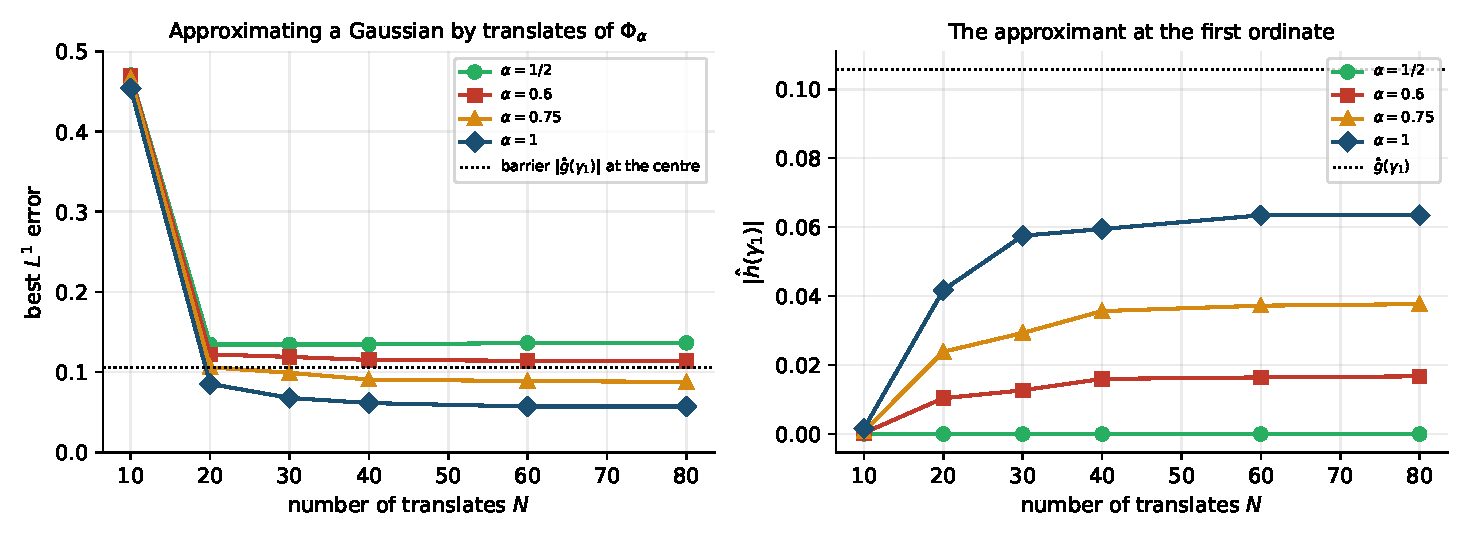
\includegraphics[width=\textwidth]{fig/bp1_wiener.pdf}
\caption{Left: best $L^1$ error against the number of translates, with the barrier at the centre. Right: the Fourier transform of the best approximant at the first ordinate, against the target $\hat g(\gamma_1)$. The data, which include $N=30$ and $N=60$, are in \texttt{wiener.json}, written by \texttt{wiener.py}, and \texttt{figs\_wiener.py} draws the figure.}
\label{wr:fig:wiener}
\end{figure}

\subsection{Salem's criterion and its P\'olya analogue}\label{wr:sec:salem}

Wiener's theorem has a dual form: for $k\in L^1(\R)$, the convolution equation $\int k(x-y)f(y)\,dy=0$ for all $x$ has a bounded solution $f\ne0$ if and only if $\hat k$ has a real zero, and then $f(y)=e^{-i\gamma y}$ is a solution for any real zero $\gamma$. Salem \cite{Salem53} used it to give one of the classical equivalents of RH: RH holds if and only if, for every $\frac12<\sigma<1$, the equation
\[
\int_{\R}\frac{e^{-\sigma y}f(y)}{e^{e^{x-y}}+1}\,dy=0\qquad(x\in\R)
\]
has no bounded solution other than $f=0$. Multiplied by $e^{\sigma x}$, it is the convolution equation with the kernel $k_\sigma(u)=e^{\sigma u}/(e^{e^u}+1)$, the Fermi Dirac function $1/(e^w+1)$ in the logarithmic variable $w=e^u$, and that substitution gives its Fourier transform,
\begin{gather*}
\hat k_\sigma(\theta)=\int_{\R}\frac{e^{\sigma u}e^{i\theta u}}{e^{e^u}+1}\,du=\int_0^\infty\frac{w^{\sigma+i\theta-1}}{e^w+1}\,dw=\Gamma(\sigma+i\theta)\,\eta(\sigma+i\theta),\\
\eta(s)=(1-2^{1-s})\zeta(s),
\end{gather*}
where $\eta$ is Dirichlet's alternating zeta function, not the Dedekind eta function of Section~\ref{ch:bpeta}. So for $\frac12<\sigma<1$ the real zeros of $\hat k_\sigma$ are exactly the ordinates of the zeros of $\zeta$ on the line $\re s=\sigma$, and Salem's criterion is Proposition~\ref{wr:prop:wiener}(4) with the Fermi Dirac kernel in place of the tilted P\'olya kernel \eqref{wr:eq:kernel}. Our family gives the P\'olya analogue directly.

\begin{corollary}\label{wr:cor:salem}
RH holds if and only if, for every $\frac12<\alpha<1$, the equation $\int_{\R}\Phi_\alpha(x-y)f(y)\,dy=0$ for all $x$ has no bounded solution $f\ne0$. At the centre the equation has the explicit bounded solutions $f(y)=\cos(\gamma y)$, one for each ordinate $\gamma$ of a zero on the critical line, because $\Xi(\gamma)=0$ there; at the basepoint one it has none.
\end{corollary}

\begin{proof}
By the dual form of Wiener's theorem with $k=\Phi_\alpha$, a bounded solution $f\ne0$ exists exactly when $\hat\Phi_\alpha(\theta)=\xi(\alpha+i\theta)$ has a real zero, that is, when $\zeta$ has a zero on the line $\re s=\alpha$. That no such zero exists for any $\alpha\in(\frac12,1)$ means that no zero has $\frac12<\re\rho<1$, which, since no zero lies on the line $\re s=1$, is RH by the symmetry $\rho\mapsto1-\rho$. At the centre $\Phi$ is even, so $\int_{\R}\Phi(x-y)\cos(\gamma y)\,dy=\Xi(\gamma)\cos(\gamma x)$, which vanishes when $\frac12+i\gamma$ is a zero; at the basepoint one $\xi(1+i\theta)\ne0$ for every real $\theta$.
\end{proof}

The two families differ at the edge of the strip. The factor $1-2^{1-s}$ in $\eta$ vanishes at $s=1+2\pi ik/\log2$ with $k\ne0$, so Salem's kernel has real Fourier zeros on the line $\sigma=1$, at $\theta=9.0647$, $18.1294$, $27.1942,\dots$, and its translates are not complete there, whereas the P\'olya family is complete at $\alpha=1$ because $\xi(1+i\theta)\ne0$. Inside the strip the two families have the same zeros and the criteria coincide. The left panel of Figure~\ref{wr:fig:salem}, computed by \texttt{salem\_riesz.py}, shows $|\eta(\sigma+i\theta)|$. At $\sigma=\frac12$ it dips to zero at every ordinate; at $\sigma=0.6$ the dips are shallow, the deepest on $(0,60]$ being $0.175$ near $\gamma_1$ and $0.189$ near $\gamma_6$; at $\sigma=0.75$ no dip goes below $0.2$; and at $\sigma=1$ the zeros of $1-2^{1-s}$ appear. The depth of the dips plays for Salem's kernel the role that $|\xi(\alpha+i\gamma)|$ plays in the cost of approximation of Proposition~\ref{wr:prop:wiener}(5), and it is of order $\sigma-\frac12$ near each ordinate.

\begin{figure}[htbp]
\centering
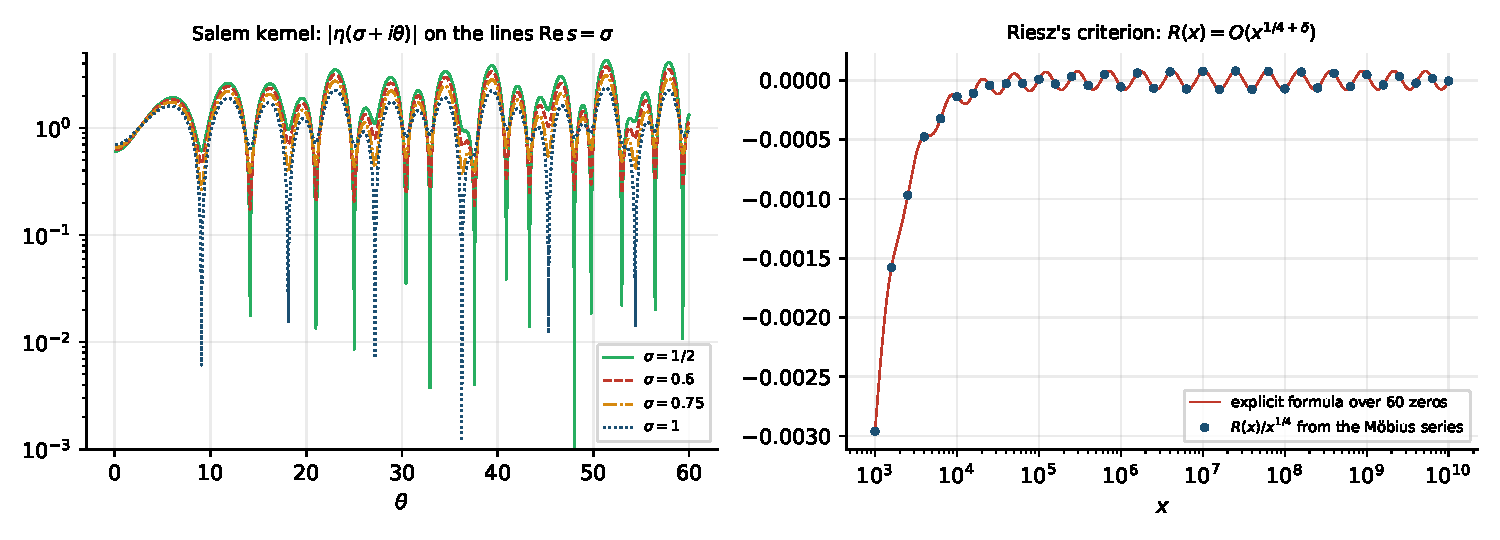
\includegraphics[width=\textwidth]{fig/bp1_salem_riesz.pdf}
\caption{Left: $|\eta(\sigma+i\theta)|$, the Fourier transform of Salem's kernel divided by $\Gamma(\sigma+i\theta)$, at $\sigma=\frac12$, $0.6$, $0.75$, $1$. Right: the Riesz function $R(x)/x^{1/4}$ from the M\"obius series and from the explicit formula \eqref{wr:eq:rieszexplicit} over $60$ zeros. The data are in \texttt{salem\_riesz.json}, written by \texttt{salem\_riesz.py}; \texttt{figs\_wiener.py} draws the figure and evaluates the explicit formula with the first $60$ ordinates in \texttt{g\_1\_400.npy} and the trivial terms in \texttt{riesz\_explicit.json}.}
\label{wr:fig:salem}
\end{figure}

\subsection{Riesz's criterion and multiplicative completeness}\label{wr:sec:riesz}

Riesz \cite{Riesz16} found the first criterion of this type, in terms of growth rather than completeness. With the M\"obius function $\mu(n)$, which is unrelated to the Thorin measure $\mu_\varepsilon$ of Section~\ref{ch:clock}, put
\begin{equation}\label{wr:eq:riesz}
R(x)=-\sum_{k\ge1}\frac{(-x)^k}{(k-1)!\,\zeta(2k)}=x\sum_{n\ge1}\frac{\mu(n)}{n^2}\,e^{-x/n^2},
\end{equation}
the second form following from $1/\zeta(2k)=\sum_n\mu(n)n^{-2k}$. Riesz proved that RH holds if and only if $R(x)=O(x^{1/4+\delta})$ for every $\delta>0$. The Mellin transform explains why: for $\frac12<\re s<1$,
\begin{equation}\label{wr:eq:rieszmellin}
\int_0^\infty R(x)\,x^{-s-1}dx=\frac{\Gamma(1-s)}{\zeta(2s)},
\end{equation}
whose poles in the strip $0<\re s<\frac12$ sit at $s=\rho/2$, and shifting the contour gives, when the zeros are simple, the explicit formula
\begin{equation}\label{wr:eq:rieszexplicit}
R(x)=\sum_\rho\frac{\Gamma(1-\rho/2)}{2\zeta'(\rho)}\,x^{\rho/2}+\sum_{k\ge1}\frac{\Gamma(1+k)}{2\zeta'(-2k)}\,x^{-k},
\end{equation}
in which the sum over the zeros is the limit of its partial sums over $|\gamma|<T_\nu$ along a suitable sequence of heights $T_\nu\to\infty$. The same argument gives the basepoint version: for $\frac12\le\alpha<1$, $\zeta$ has no zeros in $\re s>\alpha$ if and only if $R(x)=O(x^{\alpha/2+\delta})$ for every $\delta>0$. If the bound holds then, since also $|R(x)|\le\zeta(2)x$, the Mellin integral converges absolutely and is holomorphic on $\frac\alpha2<\re s<1$, so $\Gamma(1-s)/\zeta(2s)$ continues holomorphically there and $\zeta(w)\ne0$ for $\alpha<\re w<2$. Conversely, if $\zeta$ has no zeros in $\re s>\alpha$, the inversion integral $R(x)=\frac1{2\pi i}\int_{c-i\infty}^{c+i\infty}\Gamma(1-s)\zeta(2s)^{-1}x^s\,ds$, $\frac12<c<1$, moves to the line $\re s=\frac\alpha2+\delta$ without crossing a pole and gives $|R(x)|\le C_\delta x^{\alpha/2+\delta}$, provided $1/\zeta(\sigma+it)$ grows at most like a power of $|t|$ on $\sigma\ge\alpha+2\delta$, because $\Gamma(1-s)$ decays exponentially in vertical strips. The zero free half plane supplies that bound: the Borel Carath\'eodory lemma applied to $\log\zeta$ on discs centred at $2+it$ gives $\log\zeta(\sigma+it)=O_\delta(\log|t|)$ there, as in \cite[Section 14.2]{Titchmarsh} with the line $\re s=\alpha$ in place of the critical line; Proposition~\ref{ri:prop:twisted} carries out this argument in detail, for a twisted form of $R$. So Riesz's criterion runs through the same family of half planes as the constructions of Chapter~\ref{chap:basepoint}, with the growth exponent $\alpha/2$ in place of the basepoint.

In the language of this book, $R(x)/x=\sum_n\mu(n)n^{-2}e^{-x/n^2}$ is the Laplace transform of the signed M\"obius measure $\sum_n\mu(n)n^{-2}\delta_{1/n^2}$. It is a heat trace on the arithmetic side, with the M\"obius function in place of the zeros, and it is the same M\"obius series that underlies the representation of the reciprocal zeta function in Section~\ref{ch:rz1} (Theorem~\ref{rz:thm:sech}). Its sign carries no information; RH is encoded in its rate of growth, exactly as the zero free half planes are encoded in the growth of the error terms of Section~\ref{bp:sec:below}. The coefficients $1/\zeta(2k)$ of the power series of $R$ are, up to elementary factors, values of the Laplace transforms of the centre clock $T$ and of $T_1$ (Section~\ref{ri:sec:thorin}).

We computed $R(x)$ with \texttt{salem\_riesz.py} from the M\"obius series with $n\le N=10^7$, approximating
\[
R(x)\approx x\Big[\sum_{n\le N}\mu(n)n^{-2}\big(e^{-x/n^2}-1\big)+\frac6{\pi^2}\Big]
\]
to avoid the slowly converging tail, for $10\le x\le10^{12}$. Beyond $x\approx10^{10}$ the truncation at $N=10^7$ limits the accuracy: the omitted terms are about $-x^2\sum_{n>N}\mu(n)n^{-4}\approx9\times10^{-26}x^2$, that is $3\times10^{-8}$ in $R(x)/x^{1/4}$ at $x=10^{10}$ and $9\times10^{-5}$ at $x=10^{12}$. For $10^4\le x\le10^{10}$ the ratio $R(x)/x^{1/4}$ oscillates with amplitude about $1.1\times10^{-4}$, and for $10^5\le x\le10^{10}$ with amplitude $7.8\times10^{-5}$, which is the amplitude $|\Gamma(1-\rho_1/2)/\zeta'(\rho_1)|$ of the term of the first zero; the small constant reflects the decay of $\Gamma(1-\rho/2)$ along the critical line, which also makes the term of the second zero about $300$ times smaller. The larger swing near $x=10^4$ comes from the term $\Gamma(2)x^{-1}/(2\zeta'(-2))=-16.42\,x^{-1}$ of the first trivial zero, which contributes $-1.6\times10^{-4}$ to the ratio at $x=10^4$; the next two trivial zeros enter with the coefficients $\Gamma(1+k)/(2\zeta'(-2k))=125.25$ and $-508.50$ for $k=2$ and $3$. The explicit formula \eqref{wr:eq:rieszexplicit} with the first $60$ zeros and these three trivial terms reproduces the computed values to $3.1\times10^{-8}$ on $[10^3,10^{10}]$, against a signal of size up to $3\times10^{-3}$ (\texttt{riesz\_explicit.py}, output \texttt{riesz\_explicit.json}; Figure~\ref{wr:fig:salem}, right). The largest difference, at $x=10^{10}$, is the truncation error just described, and on $[10^3,10^9]$ the difference is at most $6.2\times10^{-10}$. The decay of $\Gamma(1-\rho/2)$ hides every zero above the first few from $R$. Section~\ref{ri:sec:filters} twists the M\"obius series by $(x/n^2)^{ih}$ so that it responds to the zeros near height $2h$, and computes $R$ to $x=10^{12}$ and its twists to $x=10^{10}$.

Wiener's theorem concerns translates. Its multiplicative counterpart concerns dilates, and there completeness is equivalent to RH itself. Nyman and Beurling \cite{Nyman50,Beurling55} proved that RH holds if and only if the constant function $1$ lies in the $L^2(0,1)$ closure of the span of the functions $r_\lambda(x)=\{\lambda/x\}-\lambda\{1/x\}$, $0<\lambda\le1$, where $\{\cdot\}$ is the fractional part, and B\'aez-Duarte \cite{BaezDuarte03} showed that $\lambda=1/n$ suffices. Under $x=e^{-u}$ this is a closure problem for translates in a weighted $L^2$ space on the half line, and the Mellin transform of $r_\lambda$ is $-\zeta(s)(\lambda^s-\lambda)/s$, so the zeros of $\zeta$ in the half plane $\re s>\frac12$ are exactly what obstructs the closure. The same framework governs the dilates $\sech(nx)$ of the Lai and Vere-Jones identity (Proposition~\ref{rz:prop:lvj}), which lies behind the expansion of Theorem~\ref{rz:thm:sech}: the Mellin transform of $\sech$ is $2\Gamma(s)L(s,\chi_4)$, and completeness of systems of dilates is controlled by where the associated Dirichlet series vanishes, in the sense of Beurling's periodic dilation problem and the work of Hedenmalm, Lindqvist and Seip \cite{HLS97}. How the two questions are related is the Nyman Beurling problem of Section~\ref{rz:sec:open}. Each of these completeness questions is by itself equivalent to RH or to the generalised Riemann hypothesis. The additive family of Proposition~\ref{wr:prop:wiener} is the probabilistic one, and it reaches RH only as $\alpha\downarrow\frac12$, in the same way as every other construction of Chapters~\ref{chap:basepoint} to \ref{chap:almost}.

The normal scale mixtures of this section are Brownian motion run at the clock $2T_\alpha$, and their classes are read off those of $T_\alpha$: infinite divisibility holds with no hypothesis, and the EGGC property holds exactly when $T_\alpha$ is a GGC. The completeness statements are the same zero free half planes read through Fourier transforms, and Riesz's criterion reads them through the growth of $R(x)$. Section~\ref{ch:riesz} takes up that criterion.

\section{Riesz's criterion and the Thorin path}\label{ch:riesz}

Section~\ref{wr:sec:riesz} introduced Riesz's criterion \cite{Riesz16} for the Riesz function \eqref{wr:eq:riesz} and its basepoint form, of which RH is the case $\alpha=\frac12$. Hardy and Littlewood \cite{HL16} gave a companion criterion with $\zeta(2k+1)$ in place of $\zeta(2k)$ and the exponent $-\frac14$, and the constructions of this section apply to it in the same way.

We develop the criterion in two directions. The first is computational (Section~\ref{ri:sec:filters}). The second reads the coefficients $1/\zeta(2k)$ through the clocks of Chapter~\ref{chap:basepoint}. None of this supplies the growth bound (Section~\ref{ri:sec:help}).

We keep the notation of Chapter~\ref{chap:basepoint} and Section~\ref{ch:strip} for $T=T_{1/2}$, $T_\alpha$, $\varphi_\alpha$, $H_a$, $b_\alpha$ and $v_\alpha$; in particular $b_1=\sum_\rho\rho^{-1}=0.0230957$. We write $\widetilde T=\widetilde T_1$ for the centre clock tilted by $e^{-T/4}$, as in Theorem~\ref{bp:thm:sub}, $\psi(y)=\sum_{n\le y}\Lambda(n)$ for Chebyshev's function, and
\[
\kappa_k=\frac{2k(2k-1)(k-1)!}{\pi^k},\qquad c_k=\frac1{\kappa_k\,\zeta(2k)},
\]
so that $\xi(2k)=\frac12\kappa_k\zeta(2k)$ and $c_k=\xi(1)/\xi(2k)$. The scripts named below are in \texttt{riesz\_program/code} of the archive, their outputs in \texttt{riesz\_program/data}.

\subsection{Which zeros the Riesz function sees}\label{ri:sec:filters}

On the range computed in Section~\ref{wr:sec:riesz} the Riesz function behaves exactly as RH predicts, and its fluctuations are accounted for by the known zeros, in fact by very few of them. In the explicit formula \eqref{wr:eq:rieszexplicit} a zero $\rho$ enters $R(x)$ through the term $r_\rho x^{\rho/2}$ with the weight $r_\rho=\Gamma(1-\rho/2)/(2\zeta'(\rho))$. By Stirling's formula $|\Gamma(\frac34-\frac i2\gamma)|$ decays like $e^{-\pi\gamma/4}$. The weight is $3.9\times10^{-5}$ for the first zero, whose term and that of its conjugate give the amplitude $7.8\times10^{-5}$ found in Section~\ref{wr:sec:riesz}, $2.1\times10^{-17}$ for the tenth, $1.5\times10^{-49}$ for the fiftieth and $2.2\times10^{-81}$ for the hundredth (\texttt{sens.py}, output \texttt{sens.json}; Figure~\ref{ri:fig:filters}, left). An off line zero at height $1000$ would enter with a weight near $10^{-340}$, and no feasible range of $x$ would reveal it. Riesz's criterion is equivalent to RH, but as a computational test it examines only the bottom of the spectrum.

The remedy is to change the kernel. For real $h$ put
\[
R_h(x)=x\sum_{n\ge1}\frac{\mu(n)}{n^2}\Big(\frac x{n^2}\Big)^{ih}e^{-x/n^2},\qquad x>0,
\]
so that $R_0=R$.

\begin{proposition}\label{ri:prop:twisted}
For every real $h$ and $\frac12<\re s<1$,
\[
\int_0^\infty R_h(x)\,x^{-s-1}dx=\frac{\Gamma(1-s+ih)}{\zeta(2s)} .
\]
For $\frac12\le\alpha<1$, $\zeta$ has no zeros in the half plane $\re s>\alpha$ if and only if $R_h(x)=O(x^{\alpha/2+\delta})$ for every $\delta>0$. In particular RH holds if and only if $R_h(x)=O(x^{1/4+\delta})$ for every $\delta>0$.
\end{proposition}

\begin{proof}
Term by term, $\int_0^\infty x^{1+ih}n^{-2-2ih}e^{-x/n^2}x^{-s-1}dx=n^{-2s}\Gamma(1-s+ih)$, and summing against $\mu(n)$ gives $\Gamma(1-s+ih)\sum_n\mu(n)n^{-2s}$; the interchange is justified because, with $\sigma=\re s$, the integrals of the absolute values sum to $\Gamma(1-\sigma)\zeta(2\sigma)<\infty$. Suppose that $\zeta$ has no zeros in $\re s>\alpha$. Then $1/\zeta(2s)$ is analytic in $\re s>\frac\alpha2$. By the argument of \cite[Section 14.2]{Titchmarsh} with the line of real part $\alpha$ in place of the critical line, as in Section~\ref{wr:sec:riesz}, $|1/\zeta(2s)|\le|2\im s|^{C_\delta}$ on $\re s\ge\frac\alpha2+\delta$, $|\im s|\ge5$, while $|\Gamma(1-s+ih)|$ decays like $e^{-\pi|\im s-h|/2}$ in vertical strips. So the Mellin inversion integral $R_h(x)=\frac1{2\pi i}\int_{(c)}\Gamma(1-s+ih)\zeta(2s)^{-1}x^s\,ds$, with $\frac12<c<1$, can be moved to the line $\re s=\frac\alpha2+\delta$, which gives $R_h(x)=O(x^{\alpha/2+\delta})$. Conversely, if $R_h(x)=O(x^{\alpha/2+\delta})$ as $x\to\infty$, then, since also $|R_h(x)|\le\zeta(2)\,x$, the Mellin integral converges absolutely for $\frac\alpha2+\delta<\re s<1$ and continues $\Gamma(1-s+ih)/\zeta(2s)$ analytically there. As $\Gamma$ has no zeros, $\zeta(2s)$ has no zeros with $\alpha+2\delta<\re2s<2$; since $\delta>0$ is arbitrary and $\zeta$ has no zeros with $\re s\ge1$, it has none with $\re s>\alpha$.
\end{proof}

Shifting the contour further gives, when the zeros are simple, the twisted form of the explicit formula \eqref{wr:eq:rieszexplicit}, with the sum over the zeros again the limit of its partial sums over $|\gamma|<T_\nu$ along a suitable sequence $T_\nu\to\infty$:
\begin{equation}\label{ri:eq:twexplicit}
R_h(x)=\sum_\rho\frac{\Gamma(1-\rho/2+ih)}{2\zeta'(\rho)}\,x^{\rho/2}+\sum_{k\ge1}\frac{\Gamma(1+k+ih)}{2\zeta'(-2k)}\,x^{-k}.
\end{equation}
The heights $T_\nu$ are those of \cite[Theorem 9.7]{Titchmarsh}, on which $1/\zeta(\sigma+iT_\nu)=O(T_\nu^A)$ for $-1\le\sigma\le2$; with the functional equation for $\re2s\le-1$ this makes the integrals over the horizontal segments $\im2s=\pm T_\nu$ tend to $0$. On the line $\re s=-q-\frac12$ we write $1/\zeta(2s)=\pi^{1/2-2s}\Gamma(s)/(\Gamma(\frac12-s)\zeta(1-2s))$; since $|\Gamma(1-s+ih)\Gamma(s)|\le e^{\pi|h|/2}\pi/\cosh(\pi\im s)$, $|\Gamma(\frac12-s)|\ge q!\,(\pi t/\sinh\pi t)^{1/2}$ with $t=\im s$, and $|\zeta(1-2s)|\ge2-\zeta(4)$, the integral over that line is at most $Ce^{\pi|h|/2}\pi^{2q}x^{-q-1/2}/q!$, which tends to $0$ as $q\to\infty$.

What the twist changes is the weight. Since $|\Gamma(\frac34+i(h-\gamma/2))|$ is largest when $\gamma\approx2h$ and decays like $e^{-\pi|h-\gamma/2|/2}$ away from it, $R_h$ sees the zeros in a band of width about ten around height $2h$. At $h=50$ the largest weight among the first $300$ zeros is $0.124$, at $\gamma=101.3$, where the untwisted weight is $2.9\times10^{-35}$ (Figure~\ref{ri:fig:filters}, left). With \texttt{twisted.py} we computed $R_{50}(x)$ from the M\"obius series with $\mu$ sieved to $10^7$ at forty values of $x$ in $[10^4,10^{10}]$, and compared it with \eqref{ri:eq:twexplicit} over the first $300$ zeros and three trivial terms. The two agree to $1.2\times10^{-8}$ in $|R_h(x)|/x^{1/4}$, against a signal of size up to $0.27$, and the zeros with $|\gamma-100|<15$ carry $99.9997\%$ of the modulus of the explicit formula, in the median over the forty values of $x$ (Figure~\ref{ri:fig:filters}, right).

An off line zero with real part $\beta$ near height $2h$ would contribute a term of size $x^{\beta/2}$, growing relative to the background $x^{1/4}$ by the factor $x^{(\beta-1/2)/2}$: a factor $3.2$ between $x=10^{10}$ and $x=10^{20}$ when $\beta=0.6$.

\begin{remark}\label{ri:rem:indep}
Twisted Riesz functions are not competitive with direct zero finding as a verification method. Their value is independence: they are computed from $\mu(n)$ only, with no evaluation of $\zeta$, so agreement between $R_h$ and the explicit formula over computed zeros is a check of the zeros that shares no code or method with their computation.
\end{remark}

The cost of $R(x)$ or $R_h(x)$ is dominated by sieving $\mu(n)$ to $N=K\sqrt x$. Terms with $n<\sqrt x/12$ are below $e^{-144}$ and can be omitted, and the terms with $n>N$ are summed through $\sum_n\mu(n)n^{-2}=6/\pi^2$, or $1/\zeta(2+2ih)$ for $R_h$: the script computes $R(x)/x$ as $\sum_{\sqrt x/12\le n\le N}\mu(n)n^{-2}e^{-x/n^2}+\big(6/\pi^2-\sum_{n\le N}\mu(n)n^{-2}\big)$, and the neglected remainder $\sum_{n>N}\mu(n)n^{-2}(e^{-x/n^2}-1)\approx-x\sum_{n>N}\mu(n)n^{-4}$ is of order $xN^{-7/2}$ under square root cancellation in the M\"obius tail, that is, of order $K^{-7/2}$ in $R(x)/x^{1/4}$. That cancellation is proved in the range used: the Mertens function $\sum_{n\le t}\mu(n)$ is less than $0.571\sqrt t$ in absolute value for $33\le t\le10^{16}$ \cite[Section 6.1]{Hurst18}, and partial summation then bounds the remainder in $R(x)/x^{1/4}$ by $1.1\times10^{-8}$ for $K=200$ and $1\le x\le10^{12}$. The script \texttt{riesz\_large.py} implements this with a segmented sieve and extended precision. With $K=200$ it reproduces the explicit formula over $60$ zeros and three trivial terms to about $2\times10^{-9}$ in $R(x)/x^{1/4}$ at $x=10^8$, $10^{10}$, $10^{11}$ and $10^{12}$ (\texttt{check\_large.py}). Its twisted option agrees as well: at $x=10^{10}$ with $h=50$ it gives $R_{50}(x)=37.441416-26.042495\,i$, within $3.1\times10^{-9}$ of \eqref{ri:eq:twexplicit} over $300$ zeros in $|R_h(x)|/x^{1/4}$ (\texttt{check\_large\_twisted.py}).

\begin{figure}[htbp]
\centering
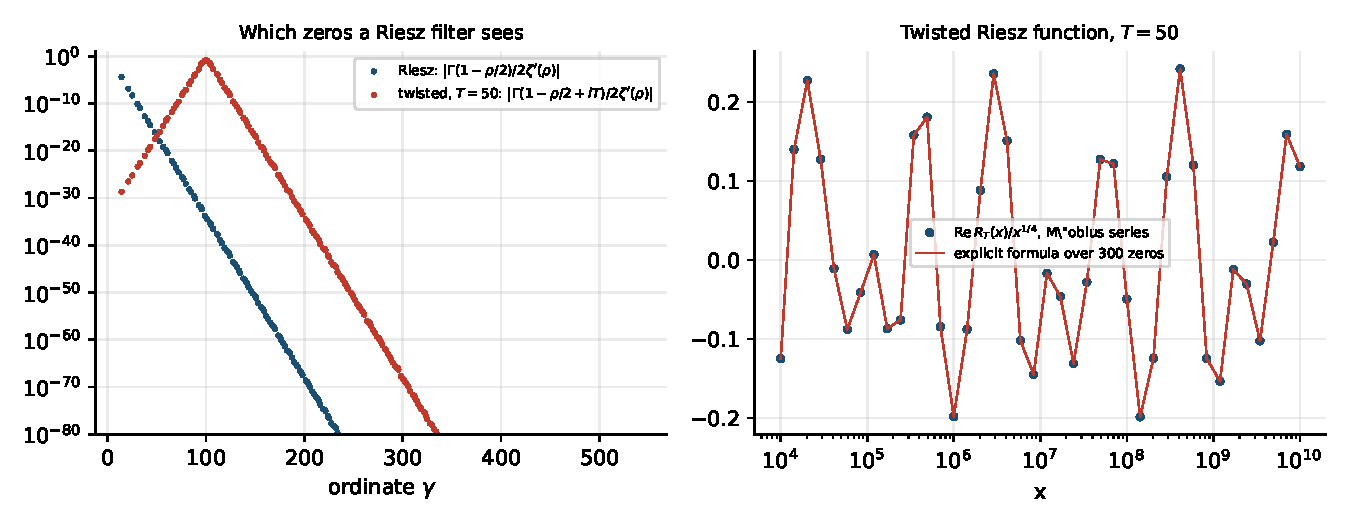
\includegraphics[width=\textwidth]{fig/ri_filters.pdf}
\caption{Left: the weights $|\Gamma(1-\rho/2)/(2\zeta'(\rho))|$ of the Riesz function and $|\Gamma(1-\rho/2+ih)/(2\zeta'(\rho))|$ of the twisted Riesz function with $h=50$, for the first $300$ zeros. Right: $\re R_{50}(x)/x^{1/4}$ from the M\"obius series against the explicit formula \eqref{ri:eq:twexplicit} over $300$ zeros. The plot writes $T$ for $h$. Data from \texttt{twisted.py}; drawn by \texttt{figs\_strategy.py}.}
\label{ri:fig:filters}
\end{figure}

\subsection{The Riesz coefficients through the centre clock}\label{ri:sec:thorin}

The Riesz coefficients are values of two Laplace transforms: that of the centre clock $T$ of \cite{P17} and that of the basepoint one clock $T_1$ (Proposition~\ref{bp:prop:thorin}).

\begin{proposition}\label{ri:prop:coef}
For every integer $k\ge1$, with no hypothesis,
\[
\frac1{\zeta(2k)}=\frac{\kappa_k}{2\xi(\frac12)}\;\E\,e^{-(2k-\frac12)^2T}=\kappa_k\;\E\,e^{-(2k-1)^2T_1}.
\]
\end{proposition}

\begin{proof}
From the definition of $\xi$, $\xi(2k)=k(2k-1)\pi^{-k}\Gamma(k)\zeta(2k)=\frac12\kappa_k\zeta(2k)$. Since $2k-\frac12>0$, the Laplace transform of $T$ at $(2k-\frac12)^2$ is $\varphi_{1/2}((2k-\frac12)^2)=\xi(\frac12)/\xi(2k)$; similarly $\E e^{-(2k-1)^2T_1}=\xi(1)/\xi(2k)$, with $\xi(1)=\frac12$.
\end{proof}

\begin{proposition}\label{ri:prop:avg}
For every $x>0$, with no hypothesis,
\[
R(x)=-\frac1{\xi(\frac12)}\;\E\Big[\sum_{k\ge1}k(2k-1)\Big(-\frac x\pi\Big)^ke^{-(2k-\frac12)^2T}\Big].
\]
\end{proposition}

\begin{proof}
Since $\kappa_k/(2(k-1)!)=k(2k-1)\pi^{-k}$, Proposition~\ref{ri:prop:coef} turns the term $-(-x)^k/((k-1)!\,\zeta(2k))$ of Riesz's series into $-\xi(\frac12)^{-1}k(2k-1)(-x/\pi)^k\,\E e^{-(2k-\frac12)^2T}$. The exchange of sum and expectation is justified by Fubini's theorem, because
\[
\sum_{k\ge1}k(2k-1)\Big(\frac x\pi\Big)^k\E\,e^{-(2k-\frac12)^2T}=\xi(\tfrac12)\sum_{k\ge1}\frac{x^k}{(k-1)!\,\zeta(2k)}<\infty .
\]
\end{proof}

The terms of the series averaged in Proposition~\ref{ri:prop:avg} decay like $e^{-4k^2T}$ rather than like $1/(k-1)!$. Table~\ref{ri:tab:check}, computed by \texttt{riesz\_thorin.py} (output \texttt{riesz\_thorin.json}), checks both propositions with $4\times10^5$ draws of $T$, generated under RH as $\sum_{\gamma>0}e_\gamma/\gamma^2$ with independent standard exponentials $e_\gamma$: the first $200$ zeros are used exactly, and the remaining terms are replaced by a gamma variable with the same mean and variance, computed from the exact power sums $\sum\gamma^{-2}$ and $\sum\gamma^{-4}$. The coefficients agree within about one standard error, and so do the values of $R$ from the M\"obius series, the power series and the clock average.

\begin{table}[htbp]
\centering\small
\begin{tabular}{cccc}
\toprule
$k$ & $1/\zeta(2k)$ & via the clock & standard error\\
\midrule
1 & 0.6079271 & 0.6079115 & 0.0000131\\
2 & 0.9239384 & 0.9238153 & 0.0001046\\
3 & 0.9829526 & 0.9826581 & 0.0002603\\
4 & 0.9959392 & 0.9954609 & 0.0004615\\
\bottomrule
\end{tabular}
\qquad
\begin{tabular}{cccc}
\toprule
$x$ & $R(x)$, M\"obius & clock average & standard error\\
\midrule
0.5 & 0.1252199 & 0.1252287 & 0.0000074\\
1 & 0.0439818 & 0.0440007 & 0.0000157\\
2 & $-0.2677934$ & $-0.2677918$ & 0.0000026\\
5 & $-0.7705597$ & $-0.7706050$ & 0.0000397\\
\bottomrule
\end{tabular}
\caption{Left: the Riesz coefficients from the clock, Proposition~\ref{ri:prop:coef}. Right: the Riesz function from the M\"obius series, which agrees with the power series to fourteen digits, and from the clock average of Proposition~\ref{ri:prop:avg}.}
\label{ri:tab:check}
\end{table}

The clock average is also far better conditioned than the power series. Riesz's power series is numerically hopeless for large $x$: its largest term is about $e^x\sqrt{x/2\pi}$, that is $10^{4344.5}$ at $x=10^4$, while $R(10^4)$ is of order $10^{-3}$. In the clock average the largest term of the inner series, $\max_kk(2k-1)(x/\pi)^ke^{-(2k-\frac12)^2T}$, is about $10^{81}$ at $x=10^4$ for the typical value $T=0.023$, and its logarithm grows like $(\log x)^2/(16T)$ instead of like $x$ (Figure~\ref{ri:fig:riesz}, right).

\begin{figure}[htbp]
\centering
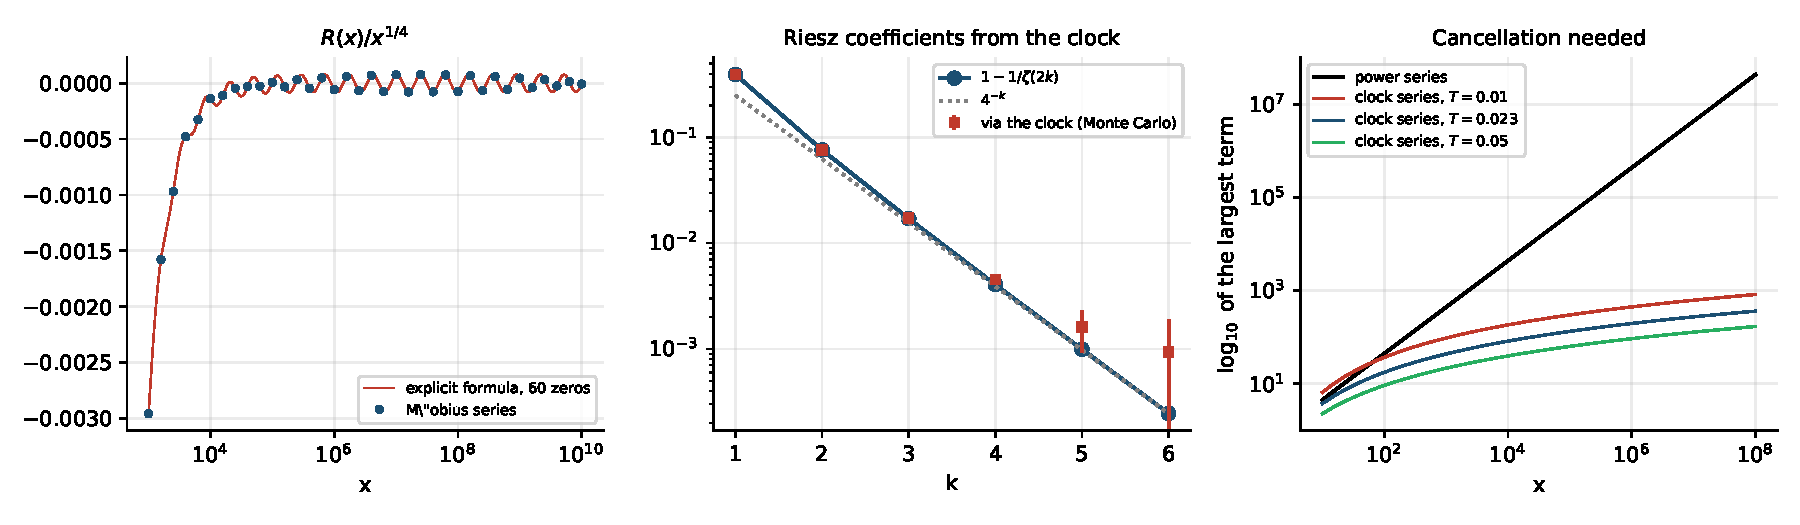
\includegraphics[width=\textwidth]{fig/ri_riesz.pdf}
\caption{Left: $R(x)/x^{1/4}$ from the M\"obius series and from the explicit formula over $60$ zeros, as in the right panel of Figure~\ref{wr:fig:salem}. Middle: $1-1/\zeta(2k)$ and its Monte Carlo value from the clock (Proposition~\ref{ri:prop:coef}), against $4^{-k}$. Right: base ten logarithm of the largest term in Riesz's power series and in the clock series of Proposition~\ref{ri:prop:avg} for $T=0.01$, $0.023$ and $0.05$.}
\label{ri:fig:riesz}
\end{figure}

\subsection{The sine squared lemma and a GGC form of Riesz's criterion}\label{ri:sec:ggc}

The computation of Proposition~\ref{ri:prop:coef} works at every basepoint between the centre and one. For $\alpha>\frac12$ the clock $T_\alpha$ exists with no hypothesis (Theorem~\ref{bp:thm:alpha}), and it is a GGC exactly when $\zeta$ has no zeros with $\re s>\alpha$ (Theorem~\ref{thm:poisson}).

\begin{proposition}[Riesz coefficients as GGC values]\label{ri:prop:ggccoef}
For every $\alpha\in[\frac12,1]$ and every integer $k\ge1$,
\[
\frac1{\zeta(2k)}=\frac{\kappa_k}{2\xi(\alpha)}\;\E\,e^{-(2k-\alpha)^2T_\alpha}.
\]
At $\alpha=1$, with no hypothesis, $T_1$ is a GGC with Thorin density $\rho_{1/2}=v_1/\pi$ in the chart $\theta=\sqrt z$, and
\[
\frac1{\zeta(2k)}=\kappa_k\exp\Big\{-\int_0^\infty\log\Big(1+\frac{(2k-1)^2}{\theta^2}\Big)\rho_{1/2}(\theta)\,d\theta\Big\}.
\]
\end{proposition}

\begin{proof}
Since $2k-\alpha>0$, the Laplace transform of $T_\alpha$ at $(2k-\alpha)^2$ is $\xi(\alpha)/\xi(2k)$, and $\xi(2k)=\frac12\kappa_k\zeta(2k)$. At $\alpha=1$, $\xi(1)=\frac12$, and the Thorin representation $\log\varphi_1(u)=-\int_0^\infty\log(1+u/\theta^2)\rho_{1/2}(\theta)\,d\theta$ of Proposition~\ref{bp:prop:thorin}, taken at $u=(2k-1)^2$, gives the second formula.
\end{proof}

\begin{remark}\label{ri:rem:hcm}
All the Riesz coefficients are samples of one GGC Laplace transform: $c_k=\varphi_1((2k-1)^2)$, where $\varphi_1(u)=\E e^{-uT_1}$. As a Laplace transform $\varphi_1$ is completely monotone, and this already makes $\log\varphi_1$ convex in $u$, by H\"older's inequality; so the slopes $(\log c_{k+1}-\log c_k)/8k$ increase with $k$. As the transform of a GGC, $\varphi_1$ is also hyperbolically completely monotone \cite[Theorem 6.1.1]{Bondesson}: for each $u>0$ the function $v\mapsto\varphi_1(uv)\varphi_1(u/v)$ is a completely monotone function of $v+1/v$. In particular it decreases as $v$ moves away from $1$, and differentiating $\log\varphi_1(uv)+\log\varphi_1(u/v)$ in $\log v$ shows that $t\mapsto\log\varphi_1(e^t)$ is concave. At the sample points this gives inequalities in the other direction: the slopes $(\log c_{k+1}-\log c_k)/\log\frac{2k+1}{2k-1}$ decrease with $k$, and $c_jc_l\le c_k^2$ whenever $(2j-1)(2l-1)=(2k-1)^2$, for instance $c_1c_5\le c_2^2$.
\end{remark}

The Thorin density $v_1/\pi$ is built from the primes by the sine squared lemma \eqref{eq:sin2}. Proposition~\ref{bp:prop:levy} writes $\log(\xi(1+s)/\xi(1))$ in the L\'evy form \eqref{bp:eq:levyform}, with the drift $b_1$ and a signed L\'evy measure $\Pi_1$ made of the gamma density, the pole of $\zeta$ and the prime atoms, and the lemma converts it term by term into the Thorin form $v_1=b_1+A+Q$ of \eqref{bp:eq:conversion}, with the gamma piece $A$ and the compensated prime piece $Q$. The L\'evy form in $s=2k-1$ is
\[
\frac1{\zeta(2k)}=\kappa_k\exp\Big\{-b_1(2k-1)-\int_0^\infty\big(e^{-(2k-1)x}-1+(2k-1)x\big)\,\Pi_1(dx)\Big\},
\]
and in the Thorin form in $u=(2k-1)^2$ the drift splits off a positive stable one half factor:
\begin{equation}\label{ri:eq:factor}
\frac1{\zeta(2k)}=\kappa_k\;e^{-b_1(2k-1)}\;\exp\Big\{-\frac1\pi\int_0^\infty\log\Big(1+\frac{(2k-1)^2}{\theta^2}\Big)\big(A(\theta)+Q(\theta)\big)\,d\theta\Big\}.
\end{equation}
This is the factorisation $T_1\stackrel d=S+T_1^\circ$ of Proposition~\ref{bp:prop:v1min} evaluated at $u=(2k-1)^2$: the middle factor is $\E e^{-(2k-1)^2S}$ for the positive stable variable $S$ of index one half with $\E e^{-uS}=e^{-b_1\sqrt u}$, and the last factor is $\E e^{-(2k-1)^2T_1^\circ}$ for the independent GGC $T_1^\circ$ with Thorin density $(A+Q)/\pi=(v_1-b_1)/\pi$.

Inserting Proposition~\ref{ri:prop:ggccoef} at $\alpha=1$ into the power series gives the Riesz function as a GGC mixture,
\begin{equation}\label{ri:eq:mixture}
R(x)=-2\,\E\Big[\sum_{k\ge1}k(2k-1)\Big(-\frac x\pi\Big)^ke^{-(2k-1)^2T_1}\Big],
\end{equation}
where the exchange of sum and expectation is justified as in Proposition~\ref{ri:prop:avg}, since $\sum_k2k(2k-1)(x/\pi)^kc_k=\sum_kx^k/((k-1)!\,\zeta(2k))<\infty$. The variable $T_1$ has two realisations. It is the tilted centre clock run through the inverse local time of a sticky Brownian motion (Theorem~\ref{bp:thm:sub} and the paragraph after it), and, like every GGC without drift \cite{JRY}, it is the Wiener gamma integral \eqref{pm:eq:wg} against the inverse of the Poisson smoothed zero count $M_{1/2}(\theta)=\pi^{-1}\int_0^\theta v_1$ (Section~\ref{pm:sec:wg}).

\begin{theorem}\label{ri:thm:ggcriesz}
For $\frac12\le\alpha<1$ the following are equivalent:
\begin{enumerate}
\item $R(x)=O(x^{\alpha/2+\delta})$ for every $\delta>0$;
\item $\zeta$ has no zeros with $\re s>\alpha$;
\item $T_{\alpha'}$ is a GGC for every $\alpha'>\alpha$;
\item for every $\alpha'>\alpha$, $v_{\alpha'}(\theta)=\re\frac{\xi'}\xi(\alpha'+i\theta)\ge0$ at every real $\theta$ for which $\alpha'+i\theta$ is not a zero of $\xi$;
\item for every $\alpha'>\alpha$ and every real $\theta$ the compensated sine squared sum
\[
\lim_{L\to\infty}\Big[\sum_{\log n\le L}\frac{\Lambda(n)}{n^{\alpha'}}\,2\sin^2\Big(\frac{\theta\log n}2\Big)-\int_0^L2\sin^2\Big(\frac{\theta x}2\Big)e^{(1-\alpha')x}\,dx\Big]
\]
converges.
\end{enumerate}
In particular RH holds if and only if $T_\alpha$ is a GGC for every $\alpha>\frac12$.
\end{theorem}

\begin{proof}
Write $\Theta=\sup\re\rho$ and $D(y)=\psi(y)-y$. Conditions (1) and (2) are equivalent by the basepoint version of Riesz's criterion (Section~\ref{wr:sec:riesz}, and Proposition~\ref{ri:prop:twisted} with $h=0$). Conditions (2) and (3) are equivalent by Theorem~\ref{thm:poisson}: $\varphi_{\alpha'}$ is the Laplace transform of a GGC exactly when $\alpha'\ge\Theta$, and this holds for every $\alpha'>\alpha$ exactly when $\Theta\le\alpha$, which is (2).

(2) implies (4), because if $\Theta\le\alpha<\alpha'$ every Cauchy kernel in $v_{\alpha'}(\theta)=\sum_\rho(\alpha'-\beta)/((\alpha'-\beta)^2+(\theta-\gamma)^2)$ has positive width (Proposition~\ref{prop:struct}). Conversely, let $\rho_0=\beta_0+i\gamma_0$ be a zero of multiplicity $m$ with $\beta_0>\alpha$. The zeros of $\xi$ are isolated, so only finitely many lie on the segment $\{\sigma+i\gamma_0:0\le\sigma\le1\}$. Let $n_0$ be the number of those other than $\rho_0$, counted with multiplicity, and choose $\eta\in(0,\beta_0-\alpha)$ with $|\beta-\beta_0|\ge2\eta$ for each of them. For $\alpha'\in(\beta_0-\eta,\beta_0)$ the point $\alpha'+i\gamma_0$ is not a zero, and Proposition~\ref{prop:struct} gives
\[
v_{\alpha'}(\gamma_0)=\frac m{\alpha'-\beta_0}+\sum_{\rho\ne\rho_0,\ \gamma=\gamma_0}\frac1{\alpha'-\beta}+\sum_{\gamma\ne\gamma_0}\frac{\alpha'-\beta}{(\alpha'-\beta)^2+(\gamma-\gamma_0)^2}.
\]
The middle sum is at most $n_0/\eta$ in absolute value. Since $\alpha'$ and $\beta$ lie in $(0,1)$, each term of the last sum is at most $(\gamma-\gamma_0)^{-2}$ in absolute value, and $\sum_{\gamma\ne\gamma_0}(\gamma-\gamma_0)^{-2}<\infty$: finitely many zeros have $0<|\gamma-\gamma_0|<1$, and for $|\gamma-\gamma_0|\ge1$ we have $(\gamma-\gamma_0)^{-2}\le5/(4+(\gamma-\gamma_0)^2)\le5(2-\beta)/((2-\beta)^2+(\gamma-\gamma_0)^2)$, a series bounded by $5v_2(\gamma_0)<\infty$. Hence $v_{\alpha'}(\gamma_0)\le m/(\alpha'-\beta_0)+n_0/\eta+\sum_{\gamma\ne\gamma_0}(\gamma-\gamma_0)^{-2}<0$ for $\alpha'$ close to $\beta_0$, and (4) fails at $(\alpha',\gamma_0)$.

(2) implies (5). This is part 1 of Proposition~\ref{bp:prop:below} at the basepoint $\alpha'$, since $\Theta\le\alpha<\alpha'$, and the argument is short. Choose $\sigma$ with $\Theta<\sigma<\alpha'$, so that $D(y)=O(y^\sigma)$ \cite{Titchmarsh}. With $f(y)=y^{-\alpha'}\,2\sin^2(\frac12\theta\log y)$ the bracket in (5) is
\[
\int_{(1,e^L]}f\,dD=f(e^L)D(e^L)-\int_1^{e^L}D(y)f'(y)\,dy,
\]
since $f(1)=0$. The boundary term tends to $0$, and the integral converges absolutely because $|f'(y)|\le(2\alpha'+|\theta|)y^{-\alpha'-1}$.

(5) implies (2). Suppose (5), and let $\rho_0$ be a zero of multiplicity $m$ with $\re\rho_0>\alpha$. Fix $\alpha'\in(\alpha,\re\rho_0)$ and $\theta\notin\mathcal E=\{\theta:\rho_0+i\theta\text{ or }\rho_0-i\theta\text{ is a zero}\}$, a countable set that contains $0$, and let $M(t)=\int_{(0,t]}(1-\cos\theta s)\,dD(e^s)$, a function of locally bounded variation. The bracket in (5) is $J(L)=\int_{(0,L]}e^{-\alpha't}dM(t)$; by hypothesis it converges as $L\to\infty$, so $J$ is bounded. For $\re w>\alpha'$, integration by parts gives
\[
\int_{(0,L]}e^{-wt}\,dM(t)=e^{-(w-\alpha')L}J(L)+(w-\alpha')\int_0^Le^{-(w-\alpha')t}J(t)\,dt,
\]
which converges as $L\to\infty$, locally uniformly in $w$, to an analytic function $F_\theta(w)$ on $\re w>\alpha'$. For $\re w>1$ the integral converges absolutely, and writing $1-\cos\theta t=1-\frac12e^{i\theta t}-\frac12e^{-i\theta t}$ gives
\begin{gather*}
F_\theta(w)=g(w)-\tfrac12g(w-i\theta)-\tfrac12g(w+i\theta),\\
g(w)=\int_{(1,\infty)}y^{-w}\,dD(y)=-\frac{\zeta'}\zeta(w)-\frac1{w-1}.
\end{gather*}
The right side, call it $\widetilde F_\theta(w)$, is meromorphic in the plane with a discrete set $\mathcal P$ of poles. On the connected open set $\Omega=\{\re w>\alpha'\}\setminus\mathcal P$ both $\widetilde F_\theta$ and $F_\theta$ are analytic, and they agree on $\re w>1$, so $\widetilde F_\theta=F_\theta$ on $\Omega$ by the identity theorem. The function $g$ is analytic at $1$, and in $\re w>0$ its only poles are the zeros of $\zeta$, each simple with residue minus its multiplicity. Since $\theta\notin\mathcal E$, $g(w\pm i\theta)$ is analytic at $\rho_0$, so $\widetilde F_\theta$ has a pole at $\rho_0$ with residue $-m\ne0$, and $|F_\theta(w)|\to\infty$ as $w\to\rho_0$ in $\Omega$. This contradicts the continuity of $F_\theta$ at $\rho_0$, where $\re\rho_0>\alpha'$. Hence no zero has real part greater than $\alpha$, which is (2).
\end{proof}

\subsection{The coefficients as killing probabilities}\label{ri:sec:kill}

For a positive random variable $X$ and an independent exponential variable $E_\lambda$ of rate $\lambda$, $\E e^{-\lambda X}=P(X<E_\lambda)$, the probability that $X$ occurs before a killing at rate $\lambda$. Propositions~\ref{ri:prop:coef} and \ref{ri:prop:ggccoef} therefore say that every Riesz coefficient is a killing probability, in two ways and with no hypothesis:
\begin{equation}\label{ri:eq:kill}
\frac1{\zeta(2k)}=\kappa_k\,P\big(T_1<E_{(2k-1)^2}\big)=\frac{\kappa_k}{2\xi(\frac12)}\,P\big(T<E_{(2k-\frac12)^2}\big).
\end{equation}
By Theorem~\ref{bp:thm:sub}, $T_1\stackrel d=\widetilde T+H_{\widetilde T/\sqrt2}$, and by the paragraph after it $T_1$ is the first time the local time at zero of a sticky Brownian motion exceeds an independent level distributed as $\widetilde T$. So $c_k=1/(\kappa_k\zeta(2k))$ is the probability that this hitting happens before an independent killing at rate $(2k-1)^2$.

The factorisation \eqref{ri:eq:factor} has the same reading. Since $\E e^{-\lambda H_a}=e^{-a\sqrt{2\lambda}}$, the stable factor is
\[
e^{-b_1(2k-1)}=P\big(H_{b_1/\sqrt2}<E_{(2k-1)^2}\big),
\]
the probability that Brownian motion reaches the level $b_1/\sqrt2=0.016331$ before it is killed. So $S\stackrel d=H_{b_1/\sqrt2}$ and $T_1\stackrel d=H_{b_1/\sqrt2}+T_1^\circ$ with $T_1^\circ$ an independent GGC. Thus $c_k=P(H_{b_1/\sqrt2}<E_{(2k-1)^2})\,P(T_1^\circ<E'_{(2k-1)^2})$, with independent exponential clocks $E$ and $E'$ of the same rate. If the exact Brownian boundary $b$ of $T_1$ is bounded at infinity, as Section~\ref{bp:sec:rs1} observes but does not prove, Lemma~\ref{bp:lem:wald} and the tail of $T_1$ make the level $b_1/\sqrt2=\sum_\rho\rho^{-1}/\sqrt2$ its Wald defect $\E\,b(T_1)$.

Under RH, if the zeros are also simple, more is true. The centre clock is then a GGC with unit atoms at the distinct points $\gamma^2$ (Proposition~\ref{prop:rigid}), hence, by Kent's theorem and Krein's inverse spectral theory (Section~\ref{sec:ch18:kent}), the hitting time of a level by the diffusion of a Krein string with Dirichlet spectrum $\{\gamma^2\}$ (Table~\ref{bh:tab:dict}). The second form of \eqref{ri:eq:kill} then says that $1/\zeta(2k)$ is proportional to the probability that this Riemann string diffusion reaches its level before it is killed at rate $(2k-\frac12)^2$. At the basepoint one, Corollary~\ref{bp:cor:kent} gives the first form the same reading under the same hypotheses.

The Riesz function becomes an alternating sum of killing probabilities,
\[
R(x)=-\sum_{k\ge1}\frac{(-x)^k}{(k-1)!}\,\kappa_k\,P\big(T_1<E_{(2k-1)^2}\big),
\]
and the criterion asks that these alternating sums grow no faster than $x^{1/4+\delta}$. The killing rates $(2k-\alpha)^2$ that the criterion needs, with $k$ in the strip $\frac14<\re k<\frac12$, are complex, and at a complex rate the Laplace transform is no longer a probability; this is the hitting time form of the obstruction of Section~\ref{ri:sec:help}.

We checked these identities with \texttt{killing.py} (output \texttt{killing.json}), using $10^6$ draws of $T_1=\widetilde T+H_{\widetilde T/\sqrt2}$ generated under RH as in Section~\ref{bp:sec:density}. Table~\ref{ri:tab:kill} compares the killing probabilities with $c_k$, and the Brownian hitting probability with $e^{-b_1(2k-1)}$; all agree within two standard errors. With the averaged killing probabilities for $k\le30$ from a second run of $10^6$ draws (\texttt{killing2.py}), the alternating sum gives $R(0.5)=0.125242$, $R(1)=0.043990$, $R(2)=-0.267895$ and $R(3)=-0.526639$, against the exact $0.125220$, $0.043982$, $-0.267793$ and $-0.526356$.

\begin{table}[htbp]
\centering\footnotesize
\begin{tabular}{@{}cccccc@{}}
\toprule
$k$ & $P(T_1<E)$, drawn & $\E e^{-(2k-1)^2T_1}$ & $c_k=\frac1{\kappa_k\zeta(2k)}$ & $P(H_{b_1/\sqrt2}<E)$ & $e^{-b_1(2k-1)}$\\
\midrule
1 & $0.95481\pm0.00021$ & $0.954928\pm0.000112$ & 0.954930 & $0.97699\pm0.00015$ & 0.97717\\
2 & $0.75965\pm0.00043$ & $0.759835\pm0.000161$ & 0.759909 & $0.93352\pm0.00025$ & 0.93306\\
3 & $0.50738\pm0.00050$ & $0.507865\pm0.000156$ & 0.507962 & $0.89098\pm0.00031$ & 0.89094\\
4 & $0.28834\pm0.00045$ & $0.288646\pm0.000122$ & 0.288731 & $0.85059\pm0.00036$ & 0.85072\\
5 & $0.14179\pm0.00035$ & $0.141473\pm0.000080$ & 0.141535 & $0.81195\pm0.00039$ & 0.81232\\
6 & $0.06045\pm0.00024$ & $0.060638\pm0.000045$ & 0.060679 & $0.77555\pm0.00042$ & 0.77565\\
\bottomrule
\end{tabular}
\caption{Riesz coefficients as killing probabilities of the basepoint one clock, and the stable factor as a Brownian hitting probability; $E$ is an independent exponential clock of rate $(2k-1)^2$, and the errors are one standard error of $10^6$ draws.}
\label{ri:tab:kill}
\end{table}

\subsection{Half Cauchy variables, the sech clock and a duality}\label{ri:sec:cauchy}

Bourgade, Fujita and Yor \cite{boBFY} derived Euler's formulae for $\zeta(2n)$ from products of Cauchy variables, and the construction gives a representation of $\zeta(2n)$ dual to that of $1/\zeta(2n)$. Let $C$ and $C'$ be independent standard Cauchy variables, so that $|C|$ and $|C'|$ are half Cauchy. By Section~\ref{bh:sec:dict}, $\E|C|^s=\sec(\pi s/2)$ for $|\re s|<1$, so $\sec^2(\pi s/2)=\E|CC'|^s$ is the moment generating function of $\log|CC'|$ on $|s|<1$. Differentiating the series $\tan z=\sum_{n\ge1}2^{2n}(2^{2n}-1)|B_{2n}|z^{2n-1}/(2n)!$ and inserting Euler's formula $\zeta(2n)=(2\pi)^{2n}|B_{2n}|/(2(2n)!)$ gives
\[
\sec^2\frac{\pi s}2=\sum_{n\ge1}\frac{8(2n-1)(1-2^{-2n})\,\zeta(2n)}{\pi^2}\,s^{2n-2},
\]
and comparing coefficients with the moment generating function,
\begin{equation}\label{ri:eq:zeta2n}
\zeta(2n)=\frac{\pi^2}{8(2n-1)(1-2^{-2n})}\;\frac{\E\big[(\log|CC'|)^{2n-2}\big]}{(2n-2)!},\qquad n\ge1.
\end{equation}

Let $\tau$ be the exit time of a standard Brownian motion from $(-1,1)$, so that $\E e^{-\lambda\tau}=1/\cosh\sqrt{2\lambda}$ (Section~\ref{bh:sec:dict}), and let $B$ be a Brownian motion independent of $\tau$. Then $\E e^{i\theta B_\tau}=\E e^{-\theta^2\tau/2}=\sech\theta$, and since $\log|C|$ has characteristic function $\sech(\pi t/2)$ (Section~\ref{bh:sec:dict}),
\[
\log|C|\stackrel d=\frac\pi2\,B_\tau .
\]
We call $\tau$ the sech clock. By the product $\cosh\sqrt{2\lambda}=\prod_{k\ge1}\big(1+8\lambda/((2k-1)^2\pi^2)\big)$ it is a GGC with unit Thorin atoms at $(2k-1)^2\pi^2/8$, the GGC $\sum_ke_k/(2k-1)^2$ of Section~\ref{bh:sec:dict} multiplied by $8/\pi^2$, and it is Kent's hitting time for the interval: the hitting time of $1$ by reflected Brownian motion started at $0$, whose eigenvalues on $[0,1]$, with reflection at $0$ and killing at $1$, are these atoms. So its spectrum is proportional to the very points $(2k-1)^2$ at which the Riesz coefficients sample the Laplace transform of $T_1$. For two independent copies, $\log|CC'|\stackrel d=\frac\pi2B_{\tau+\tau'}$. Combining \eqref{ri:eq:zeta2n} with Proposition~\ref{ri:prop:ggccoef} gives a duality between the two clocks,
\begin{equation}\label{ri:eq:duality}
\frac{\E\big[(\log|CC'|)^{2k-2}\big]}{(2k-2)!}\;\E\,e^{-(2k-1)^2T_1}=\frac{8(2k-1)(1-2^{-2k})}{\pi^2\kappa_k},
\end{equation}
in which a moment of Brownian motion stopped at a sum of two independent sech clocks, times a killing probability of the basepoint one clock, is an elementary constant.

We checked the moment formula \eqref{ri:eq:zeta2n} exactly through the Taylor coefficients of $\sec^2$, where it reproduces $\zeta(2)$, $\zeta(4)$, $\zeta(6)$ and $\zeta(8)$ to ten digits. The duality \eqref{ri:eq:duality} holds with the killing probabilities simulated in the second run of Section~\ref{ri:sec:kill}: the products are $0.95508$, $1.87524$, $2.06191$ and $1.63889$ for $k=1,\dots,4$, against $0.95493$, $1.87500$, $2.06167$ and $1.63851$.

The duality is structural rather than quantitative: $\zeta(2k)$ as a moment lives at the integers, while Riesz's criterion needs $1/\zeta(2s)$ inside the strip. The half Cauchy law also enters the book through Bosch's theorem \cite{boBosch} (Section~\ref{ch:boschA}), whose dictionary, Table~\ref{bh:tab:dict}, pairs the odd integers $2k-1$ with the ordinates $\gamma$.

\subsection{Why the representation cannot supply the growth bound}\label{ri:sec:help}

The representations of Sections~\ref{ri:sec:thorin} to \ref{ri:sec:cauchy} are exact, and all of them except the Kent string readings of Section~\ref{ri:sec:kill} hold with no hypothesis. They do not supply the bound $R(x)=O(x^{1/4+\delta})$, for four reasons.
\begin{enumerate}
\item The integer values carry almost no information. The growth of $R$ is fixed by the Mellin transform $\Gamma(1-s)/\zeta(2s)$, that is, by the analytic interpolation of $k\mapsto1/\zeta(2k)$ to complex $k$ with $\frac14<\re k<\frac12$. At the integers $1/\zeta(2k)=1-4^{-k}+O(9^{-k})$, and these values, which Proposition~\ref{ri:prop:coef} represents, determine the interpolation only through its analytic continuation.
\item The representation interpolates only on one side of the line $\re2k=\alpha$, and as an expectation only on a cone. For complex $k$ the expectation $\E e^{-(2k-\alpha)^2T_\alpha}$ is finite exactly when $\re(2k-\alpha)^2\ge0$, because $T_\alpha$ has a tail of order $t^{-1/2}$ (Theorem~\ref{bp:thm:alpha}) and no exponential moments; there it equals $\varphi_\alpha((2k-\alpha)^2)=\xi(\alpha)/\xi(\alpha+\sqrt{(2k-\alpha)^2})$, and the principal square root equals $2k-\alpha$ only when $\re(2k-\alpha)>0$. So the representation through $T_\alpha$ returns $\xi(\alpha)/\xi(2k)$ as an expectation on the cone $|\im2k|\le\re2k-\alpha$, and on the rest of the half plane $\re2k>\alpha$ only through the analytic continuation of $\varphi_\alpha$, which is analytic there exactly when no zero lies to the right of $\alpha$. It is a GGC representation with no hypothesis only for $\alpha\ge1$, that is, on the half plane $\re2k>1$ of absolute convergence, where the criterion carries no information. To reach $\frac12<\re2k<1$ one needs a basepoint $\alpha<1$, and $T_\alpha$ is a GGC there exactly when $\zeta$ has no zeros in $\re s>\alpha$.
\item The centre clock's Laplace integral converges only up to its first singularity, which under RH is at $-\gamma_1^2$. In the $k$ plane, with $u=(2k-\frac12)^2$, the region $\re u>-\gamma_1^2$ is a neighbourhood of the segment $|\im2k|<\gamma_1$ of the critical line $\re2k=\frac12$, not the strip; beyond it one needs analytic continuation, which is again a statement about the zeros.
\item Positivity does not survive. Each coefficient becomes a positive average, but the series is alternating, and the bound requires, at $x=10^4$ and $T=0.023$, the cancellation of terms as large as $10^{81}$ after averaging. No monotonicity or positivity argument controls that cancellation; it is carried by the oscillating terms $x^{\rho/2}$ of the explicit formula.
\end{enumerate}

What would help is what the basepoint version of the criterion (Proposition~\ref{ri:prop:twisted} with $h=0$) requires: an analytic, and ideally positive, representation of $1/\zeta(2s)$ on whole vertical lines of the strip $\frac14<\re s<\frac12$. A representation of the Thorin kind that is positive there is a GGC at a basepoint below one, that is, a zero free half plane. The Thorin representation of the Riesz coefficients is therefore an exact reformulation, with better cancellation and a probabilistic reading, that reaches the criterion only through the same step that every other construction of Chapters~\ref{chap:basepoint} to \ref{chap:almost} requires. At a basepoint $\frac12<\alpha<1$, zero density estimates bound the number of Mellin poles to the right of the line $\re s=\alpha/2$ up to any given height, as they bound the negative part of $v_\alpha/\pi$ (Theorem~\ref{ag:thm:almost}), but a single such pole breaks the bound $R(x)=O(x^{\alpha/2+\delta})$ for small $\delta$.


\section{The squarefree series and the clock}\label{sec:sqfree}

Riesz's criterion (Sections~\ref{wr:sec:riesz} and \ref{ch:riesz}) reads RH from a function whose Mellin transform is $\Gamma(1-s)/\zeta(2s)$. The squarefree integers carry the same reciprocal $1/\zeta(2s)$. Their Dirichlet series is
\begin{equation}\label{eq:sqfree:D}
D(s)=\sum_{n\ge1}\frac{\mu(n)^2}{n^s}=\prod_p\big(1+p^{-s}\big)=\frac{\zeta(s)}{\zeta(2s)},\qquad\re s>1,
\end{equation}
whose singularities in the half plane $\re s>0$ are the pole at $s=1$ and the poles at the points $\rho/2$ at which $\zeta(\rho/2)\ne0$ (all of them under RH), and the number $Q(x)$ of squarefree integers up to $x$ oscillates about $6x/\pi^2$ on the scale $x^{1/4}$ that these poles set when they lie on the line $\re s=\frac14$, that is under RH. This section follows the first author's note \cite{P26sqf}, which starts from a Math StackExchange thread \cite{MSE2063166} on the partial sums of $\mu(n)^2n^{-\alpha}$ over $\mathbb Q$ and over number fields. Write $\Delta(x)=Q(x)-6x/\pi^2$ for the error. The bound $\Delta(x)=O(x^{1/4+\varepsilon})$ is open even under RH, but it is equivalent to RH once the count is smoothed by an exponential or a Gamma(2) law, and in mean square; the order $x^{1/4}$ is attained with no hypothesis; and the bound for the count smoothed by a Gamma($n$) law loses a factor $n^{1/8}$, which still gives $\Delta(x)=O(x^{2/5+\varepsilon})$ under RH (Sections~\ref{sec:sqfree:smooth} and \ref{sec:sqfree:meansq}). The P\'olya kernels of the Dedekind zeta functions of imaginary quadratic fields, whose positivity can fail, are in Section~\ref{sec:sqfree:quad} of Chapter~\ref{chap:probability}.

We keep the notation of Section~\ref{ch:clock} for the P\'olya variable $X$, with $\E e^{sX}=\xi(\frac12+s)/\xi(\frac12)$, the clock $T$, $G(u)=\xi(\frac12+\sqrt u)/\xi(\frac12)$, the numbers $a_k=-(\rho_k-\frac12)^2$, the heat trace $W(t)=\sum_ke^{-a_kt}$ and the measure $U_{\RH}$, and the notation of Section~\ref{bp:sec:mellin} for the tilted variables $V_\alpha$, with $\E e^{sV_\alpha}=\xi(\alpha+s)/\xi(\alpha)$, and $b_\alpha=\frac{\xi'}\xi(\alpha)=\E V_\alpha$. Throughout, $\mu$ is the M\"obius function, $M(t)=\sum_{d\le t}\mu(d)$ is the Mertens function, $\{y\}$ is the fractional part of $y$, and
\[
Q(x)=\sum_{n\le x}\mu(n)^2,\qquad \Delta(x)=Q(x)-\frac6{\pi^2}\,x .
\]

\subsection{The thread: Perron's formula and an elementary method}\label{sec:sqfree:thread}

The question asks for the behaviour as $x\to\infty$ of
\[
S_\alpha(x)=\sum_{N(\mathfrak a)\le x}\frac{\mu(\mathfrak a)^2}{N(\mathfrak a)^\alpha},
\]
the sum running over the integral ideals $\mathfrak a$ of a number field $K$, with $\mu$ the M\"obius function of ideals and $N$ the norm, and, in a comment, for its expansion at $\alpha=1$. Over $\mathbb Q$, $S_\alpha(x)=\sum_{n\le x}\mu(n)^2n^{-\alpha}$, and another comment points to Abel summation from the classical count
\begin{equation}\label{eq:sqfree:Q}
Q(x)=\frac6{\pi^2}\,x+O(\sqrt x).
\end{equation}
The accepted answer applies Perron's formula over $K$, and the other answer carries out the elementary method over $\mathbb Q$. Neither evaluates the constant at $\alpha=1$.

Since $\mu(\mathfrak p^k)^2$ is $1$ for $k\le1$ and $0$ for $k\ge2$, the Euler factor of $\sum_{\mathfrak a}\mu(\mathfrak a)^2N(\mathfrak a)^{-s}$ at a prime ideal $\mathfrak p$ is $1+N(\mathfrak p)^{-s}=(1-N(\mathfrak p)^{-2s})/(1-N(\mathfrak p)^{-s})$, so the series is $\zeta_K(s)/\zeta_K(2s)$, with $\zeta_K$ the Dedekind zeta function of $K$, and
\begin{equation}\label{eq:sqfree:perron}
S_\alpha(x)=\frac1{2\pi i}\int_{\sigma-i\infty}^{\sigma+i\infty}\frac{\zeta_K(\alpha+s)}{\zeta_K(2\alpha+2s)}\,x^s\,\frac{ds}s,\qquad \sigma>\max\{1-\alpha,0\}.
\end{equation}

The integrand of \eqref{eq:sqfree:perron} has a simple pole at $s=1-\alpha$, a pole at $s=0$, and poles at the points $s=\rho/2-\alpha$ for the zeros $\rho$ of $\zeta_K$, trivial and nontrivial, at which $\zeta_K(\rho/2)\ne0$. Let $c_K=\lim_{s\to1}(s-1)\zeta_K(s)=2^{r_1}(2\pi)^{r_2}hR/(w\sqrt{|d_K|})$ be the residue of the class number formula.

\emph{The case $\alpha\ne1$.} The residue at $s=1-\alpha$ is $c_Kx^{1-\alpha}/((1-\alpha)\zeta_K(2))$, as the accepted answer states, and the residue at $s=0$, which it lists among the poles but does not compute, is $\zeta_K(\alpha)/\zeta_K(2\alpha)$, the value of the continued series. Over $\mathbb Q$, for $\alpha>\frac12$ and $\alpha\ne1$, the two residues are the main terms of
\begin{equation}\label{eq:sqfree:alpha}
\sum_{n\le x}\frac{\mu(n)^2}{n^\alpha}=\frac6{\pi^2}\,\frac{x^{1-\alpha}}{1-\alpha}+\frac{\zeta(\alpha)}{\zeta(2\alpha)}+O\big(x^{\frac12-\alpha}\big).
\end{equation}
For a proof, Abel summation and \eqref{eq:sqfree:Q} give, for $\alpha>\frac12$, $\alpha\ne1$,
\begin{equation}\label{eq:sqfree:abel}
\sum_{n\le x}\frac{\mu(n)^2}{n^\alpha}=\frac6{\pi^2}\,\frac{x^{1-\alpha}}{1-\alpha}+\Big(\alpha\int_1^\infty\frac{\Delta(t)}{t^{\alpha+1}}\,dt-\frac6{\pi^2}\,\frac\alpha{1-\alpha}\Big)+\frac{\Delta(x)}{x^\alpha}-\alpha\int_x^\infty\frac{\Delta(t)}{t^{\alpha+1}}\,dt .
\end{equation}
The last two terms are $O(x^{\frac12-\alpha})$, and the bracket is $D(\alpha)$, because $D(s)=s\int_1^\infty Q(t)t^{-s-1}dt=\frac6{\pi^2}\frac s{s-1}+s\int_1^\infty\Delta(t)t^{-s-1}dt$ for $\re s>1$ and the right side is analytic in $\re s>\frac12$ apart from $s=1$. For $\frac12<\alpha<1$ the constant is negative (Corollary~\ref{cor:sqfree:sign}). Write $\mathcal E_\alpha(x)$ for the left side of \eqref{eq:sqfree:alpha} minus its two main terms, so that by \eqref{eq:sqfree:abel}
\begin{equation}\label{eq:sqfree:Ealpha}
\mathcal E_\alpha(x)=\frac{\Delta(x)}{x^\alpha}-\alpha\int_x^\infty\frac{\Delta(t)}{t^{\alpha+1}}\,dt .
\end{equation}


\emph{The case $\alpha=1$.} The poles at $1-\alpha$ and at $0$ merge into a double pole at $s=0$ of $\zeta_K(1+s)\zeta_K(2+2s)^{-1}e^{s\log x}/s$. The accepted answer computes the coefficient of $\log x$ and says that the constant term is much more complicated, at least when $K\ne\mathbb Q$. It is explicit. Define the Euler Kronecker constant $\gamma_K$ of $K$ by $\zeta_K(s)=c_K/(s-1)+c_K\gamma_K+O(s-1)$ \cite{Ihara06}, so that $\gamma_{\mathbb Q}=\gamma_E$. With $1/\zeta_K(2+2s)=\zeta_K(2)^{-1}\big(1-2s\,\zeta_K'(2)/\zeta_K(2)+O(s^2)\big)$ the residue at $s=0$ is
\begin{equation}\label{eq:sqfree:alpha1K}
\frac{c_K}{\zeta_K(2)}\big(\log x+C_K\big),\qquad C_K=\gamma_K-2\,\frac{\zeta_K'(2)}{\zeta_K(2)} .
\end{equation}


\emph{The elementary method.} The identity $\mu(n)^2=\sum_{d^2\mid n}\mu(d)$, the coefficientwise form of $D(s)=\zeta(s)\cdot\zeta(2s)^{-1}$, gives
\begin{equation}\label{eq:sqfree:Qd}
Q(x)=\sum_{d\le\sqrt x}\mu(d)\Big\lfloor\frac x{d^2}\Big\rfloor=x\sum_{d\le\sqrt x}\frac{\mu(d)}{d^2}-\sum_{d\le\sqrt x}\mu(d)\Big\{\frac x{d^2}\Big\},
\end{equation}
and since $\sum_{d>\sqrt x}d^{-2}=O(x^{-1/2})$ and the last sum has at most $\sqrt x$ terms, each in $[0,1)$, this is \eqref{eq:sqfree:Q}. The second answer then sets
\begin{gather*}
B(x)=\sum_{n\le x}\Big(\mu(n)^2-\frac6{\pi^2}\Big)=O(\sqrt x),\\
D_0(s)=\sum_{n\ge1}\frac{\mu(n)^2-6/\pi^2}{n^s}=D(s)-\frac6{\pi^2}\,\zeta(s).
\end{gather*}
By Abel summation, $D_0(s)=\lim_{x\to\infty}\big(B(x)x^{-s}+s\int_1^xB(t)t^{-s-1}dt\big)$ converges for $\re s>\frac12$, so $\sum_{n\le x}\mu(n)^2/n=\frac6{\pi^2}(\log x+\gamma_E)+D_0(1)+o(1)$, and there the answer stops. Since $D_0(s)=\zeta(s)\big(\zeta(2s)^{-1}-\zeta(2)^{-1}\big)$ and $\zeta$ has a simple pole with residue $1$ at $s=1$,
\[
D_0(1)=\lim_{s\to1}\zeta(s)\Big(\frac1{\zeta(2s)}-\frac1{\zeta(2)}\Big)=-\frac{2\zeta'(2)}{\zeta(2)^2}=0.69298946940360442669,
\]
in agreement with \eqref{eq:sqfree:alpha1K} at $K=\mathbb Q$, where $c_{\mathbb Q}=1$ and $\gamma_{\mathbb Q}=\gamma_E$.

\begin{proposition}\label{prop:sqfree:alpha1}
\textup{(i)} Let $K$ be a number field of degree $n\ge2$. As $x\to\infty$,
\[
\sum_{N(\mathfrak a)\le x}\frac{\mu(\mathfrak a)^2}{N(\mathfrak a)}=\frac{c_K}{\zeta_K(2)}\big(\log x+C_K\big)+O\big(x^{-1/n}\log x\big).
\]
\textup{(ii)} Over $\mathbb Q$,
\begin{equation}\label{eq:sqfree:alpha1}
\begin{gathered}
\sum_{n\le x}\frac{\mu(n)^2}n=\frac6{\pi^2}\big(\log x+C\big)+O\big(x^{-1/2}\big),\\
C=\gamma_E-2\,\frac{\zeta'(2)}{\zeta(2)}=24\log A-\gamma_E-2\log2\pi,
\end{gathered}
\end{equation}
where $A$ is the Glaisher Kinkelin constant; $C=1.717137651090598473406241$ and $\frac6{\pi^2}C=1.0438945157119382974$. Moreover $\mathcal E_1(x)=\sum_{n\le x}\mu(n)^2/n-\frac6{\pi^2}(\log x+C)$ is given by \eqref{eq:sqfree:Ealpha} with $\alpha=1$, and
\[
\int_1^\infty\frac{\Delta(t)}{t^2}\,dt=\frac6{\pi^2}\,(C-1)=0.43596741385791166874 .
\]
\end{proposition}

\begin{proof}
(i) The number of ideals of norm at most $y$ is $c_Ky+O(y^{1-1/n})$ \cite[Chapter~VI]{Lang94}, so by Abel summation $L(y)=\sum_{N(\mathfrak c)\le y}N(\mathfrak c)^{-1}=c_K(\log y+\gamma_K)+O(y^{-1/n})$ for $y\ge1$, the constant being the one in the Laurent expansion of $\zeta_K$ at $s=1$. Since $\mu(\mathfrak a)^2=\sum_{\mathfrak b^2\mid\mathfrak a}\mu(\mathfrak b)$, as one checks on prime powers,
\begin{align*}
\sum_{N(\mathfrak a)\le x}\frac{\mu(\mathfrak a)^2}{N(\mathfrak a)}&=\sum_{N(\mathfrak b)\le\sqrt x}\frac{\mu(\mathfrak b)}{N(\mathfrak b)^2}\,L\Big(\frac x{N(\mathfrak b)^2}\Big)\\
&=c_K\sum_{N(\mathfrak b)\le\sqrt x}\frac{\mu(\mathfrak b)}{N(\mathfrak b)^2}\big(\log x+\gamma_K-2\log N(\mathfrak b)\big)\\
&\qquad+O\Big(x^{-1/n}\sum_{N(\mathfrak b)\le\sqrt x}N(\mathfrak b)^{-2+2/n}\Big).
\end{align*}
The last sum is $O(\log x)$, since $-2+2/n\le-1$. Completing the sums over $\mathfrak b$ costs $O(x^{-1/2}\log x)$, which is $O(x^{-1/n}\log x)$ as $n\ge2$, since $\sum_{N(\mathfrak b)>Y}N(\mathfrak b)^{-2}\log N(\mathfrak b)=O(Y^{-1}\log Y)$, and the completed sums are $\sum_{\mathfrak b}\mu(\mathfrak b)N(\mathfrak b)^{-2}=1/\zeta_K(2)$ and $\sum_{\mathfrak b}\mu(\mathfrak b)\log N(\mathfrak b)\,N(\mathfrak b)^{-2}=\zeta_K'(2)/\zeta_K(2)^2$, which give \eqref{eq:sqfree:alpha1K}.

(ii) By Abel summation, $\sum_{n\le x}\mu(n)^2/n=Q(x)/x+\int_1^xQ(t)t^{-2}dt$, and inserting $Q(t)=6t/\pi^2+\Delta(t)$ gives
\[
\sum_{n\le x}\frac{\mu(n)^2}n=\frac6{\pi^2}\log x+\frac6{\pi^2}+\int_1^\infty\frac{\Delta(t)}{t^2}\,dt+\frac{\Delta(x)}x-\int_x^\infty\frac{\Delta(t)}{t^2}\,dt,
\]
whose last two terms are $O(x^{-1/2})$ by \eqref{eq:sqfree:Q}. So the formula holds with some constant, and the constant is identified through $D$: for $\re s>1$, $\int_1^\infty\Delta(t)t^{-s-1}dt=D(s)/s-\frac6{\pi^2}\frac1{s-1}$, and $D(s)=\frac6{\pi^2}\zeta(s)+D_0(s)=\frac6{\pi^2}\big(\frac1{s-1}+\gamma_E-2\frac{\zeta'(2)}{\zeta(2)}\big)+O(s-1)$, so that $\int_1^\infty\Delta(t)t^{-2}dt=\frac6{\pi^2}(C-1)$ by continuity at $s=1$. This gives \eqref{eq:sqfree:alpha1} and the formula for $\mathcal E_1$, and the classical evaluation $\zeta'(2)/\zeta(2)=\gamma_E+\log2\pi-12\log A$ gives the second form of $C$.
\end{proof}

The sieve \texttt{sqfree\_sieve.py} gives $Q(2\times10^8)=121585426$. Table~\ref{tab:sqfree:sharp} shows that $\mathcal E_1(x)$ is of order $x^{-3/4}$ and $\Delta(x)$ of order $x^{1/4}$, the sizes that the poles at $\rho/2-1$ and $\rho/2$ predict under RH (Section~\ref{sec:sqfree:atoms}).

\begin{table}[htbp]
\centering\small
\begin{tabular}{rrrrrr}
\toprule
$x$ & $Q(x)$ & $\Delta(x)/x^{1/4}$ & $\mathcal E_1(x)$ & $\mathcal E_1(x)\,x^{3/4}$ & $\mathcal E_{3/4}(x)\,x^{1/4}$\\
\midrule
$10^3$ & $608$ & $0.0130$ & $-9.130\times10^{-4}$ & $-0.162$ & $-0.0291$\\
$10^4$ & $6083$ & $0.3729$ & $3.031\times10^{-4}$ & $0.303$ & $0.0296$\\
$10^5$ & $60794$ & $0.0725$ & $-2.308\times10^{-6}$ & $-0.0130$ & $-0.00031$\\
$10^6$ & $607926$ & $-0.0348$ & $-1.665\times10^{-6}$ & $-0.0526$ & $-0.00177$\\
$10^7$ & $6079291$ & $0.3553$ & $1.729\times10^{-6}$ & $0.308$ & $0.00561$\\
$10^8$ & $60792694$ & $-0.1619$ & $-1.737\times10^{-7}$ & $-0.174$ & $-0.00174$\\
\bottomrule
\end{tabular}
\caption{The sharp counts: the number $Q(x)$ of squarefree integers up to $x$, the normalised error $\Delta(x)/x^{1/4}$, the error $\mathcal E_1(x)$ of \eqref{eq:sqfree:alpha1}, which confirms the constant $C$, also multiplied by $x^{3/4}$, and the error $\mathcal E_{3/4}(x)$ of \eqref{eq:sqfree:alpha} at $\alpha=\frac34$ multiplied by $x^{1/4}$. Computed by \texttt{sqfree\_sieve.py}; the sums of reciprocals are checked in extended precision.}
\label{tab:sqfree:sharp}
\end{table}

\subsection{The P\'olya form of the series and the constant}\label{sec:sqfree:polya}



\begin{lemma}\label{lem:sqfree:gamma}
For all $s$,
\[
D(s)=\Gamma_{\mathrm{sq}}(s)\,\frac{\xi(s)}{\xi(2s)},\qquad \Gamma_{\mathrm{sq}}(s)=\frac{2s-1}{s-1}\,2^s\pi^{-(s+1)/2}\,\Gamma\Big(\frac{s+1}2\Big).
\]
\end{lemma}

\begin{proof}
By the definition of $\xi$, $\zeta(s)/\zeta(2s)=\frac{\xi(s)}{\xi(2s)}\cdot\frac{2(2s-1)}{s-1}\,\pi^{-s/2}\,\frac{\Gamma(s)}{\Gamma(s/2)}$, and the duplication formula $\Gamma(s)=2^{s-1}\pi^{-1/2}\Gamma(\frac s2)\Gamma(\frac{s+1}2)$ gives the factor $\Gamma_{\mathrm{sq}}$.
\end{proof}

The script \texttt{sqfree\_constants.py} checks the lemma at $s=3$, $0.3+2.1i$, $\frac34$ and $-1.5$, with relative errors below $5\times10^{-41}$.

\begin{proposition}\label{prop:sqfree:polya}
For every $s$ with $\xi(2s)\ne0$,
\[
\sum_{n\ge1}\frac{\mu(n)^2}{n^s}=\Gamma_{\mathrm{sq}}(s)\,\frac{\E e^{(s-\frac12)X}}{\E e^{(2s-\frac12)X}} ,
\]
the left side read as the continuation $D(s)$ where the series diverges.
\end{proposition}

\begin{proof}
Lemma~\ref{lem:sqfree:gamma} and \eqref{eq:ch2:mgf}, which gives $\xi(s)=\xi(\frac12)\E e^{(s-\frac12)X}$ and $\xi(2s)=\xi(\frac12)\E e^{(2s-\frac12)X}$.
\end{proof}



\begin{corollary}\label{cor:sqfree:sign}
For real $\alpha\notin\{1,\frac12,-1,-3,-5,\dots\}$ the sign of $\zeta(\alpha)/\zeta(2\alpha)$ is the sign of $\frac{2\alpha-1}{\alpha-1}\Gamma(\frac{\alpha+1}2)$. It is positive for $\alpha>1$ and for $-1<\alpha<\frac12$, negative for $\frac12<\alpha<1$, and equal to $(-1)^k$ on the interval $(-2k-1,-2k+1)$ for $k\ge1$.
\end{corollary}

\begin{proof}
At real $\alpha$ the ratio of moment generating functions in Proposition~\ref{prop:sqfree:polya} is positive, and so is $2^\alpha\pi^{-(\alpha+1)/2}$. The rational factor is positive except on $(\frac12,1)$, and $\Gamma(\frac{\alpha+1}2)$ has the sign $(-1)^k$ when $\frac{\alpha+1}2\in(-k,-k+1)$, that is when $\alpha\in(-2k-1,-2k+1)$.
\end{proof}

At the even negative integers both $\zeta(\alpha)$ and $\zeta(2\alpha)$ vanish and the quotient keeps its sign through them. At $\alpha=\frac34$, inside the interval where the series diverges, $\Gamma_{\mathrm{sq}}(\frac34)=-1.34612167295$, $\E e^{X/4}=1.00144503253351$ and $\E e^X=1.02335500958202$, the last two by the trapezoid rule on the P\'olya kernel \eqref{eq:ch2:Phi}; the ratio $0.978590052481$ multiplies $\Gamma_{\mathrm{sq}}(\frac34)$ to $-1.31730127858=\zeta(\frac34)/\zeta(\frac32)$.

\begin{theorem}\label{thm:sqfree:const}
The constant of \eqref{eq:sqfree:alpha1} is
\[
C=2+\log2-\tfrac12\log\pi-\tfrac12\gamma_E+b_1-2b_2=2+\log2-\tfrac12\log\pi-\tfrac12\gamma_E+\E V_1-2\,\E V_2 .
\]
With no hypothesis on the zeros,
\begin{equation}\label{eq:sqfree:zeropart}
\begin{split}
b_1-2b_2&=\frac{G'}G\Big(\frac14\Big)-6\,\frac{G'}G\Big(\frac94\Big)=\sum_k\Big(\frac1{\frac14+a_k}-\frac6{\frac94+a_k}\Big)\\
&=\int_0^\infty\big(e^{-t/4}-6e^{-9t/4}\big)\,W(t)\,dt,
\end{split}
\end{equation}
the sum running over the pairs $\{\rho,1-\rho\}$ and converging absolutely. Under RH, $a_k=\gamma_k^2$ and $b_1-2b_2=\int\big((z+\frac14)^{-1}-6(z+\frac94)^{-1}\big)\,U_{\RH}(dz)$, a combination of two values of the Stieltjes transform of the Thorin measure of the clock.
\end{theorem}

\begin{proof}
By the proof of Proposition~\ref{prop:sqfree:alpha1}, $(s-1)D(s)=\frac6{\pi^2}\big(1+C(s-1)+O((s-1)^2)\big)$, so $C$ is the derivative of $\log((s-1)D(s))$ at $s=1$. By Proposition~\ref{prop:sqfree:polya},
\begin{align*}
\log\big((s-1)D(s)\big)&=\log(2s-1)+s\log2-\tfrac{s+1}2\log\pi+\log\Gamma\big(\tfrac{s+1}2\big)\\
&\qquad+\log\E e^{(s-\frac12)X}-\log\E e^{(2s-\frac12)X}.
\end{align*}
At $s=1$ the derivatives of the first four terms are $2$, $\log2$, $-\frac12\log\pi$ and $\frac12\psi(1)=-\frac12\gamma_E$, with $\psi$ the digamma function here. The derivative of $\log\E e^{(s-\frac12)X}$ at $s=1$ is $\E Xe^{X/2}/\E e^{X/2}$, the mean of $X$ tilted by $e^{X/2}$, which is $\E V_1=b_1$ (Section~\ref{bp:sec:mellin}); likewise the last term gives $-2\E V_2=-2b_2$. For the zero form, differentiating $\log G(w^2)=\log\xi(\frac12+w)-\log\xi(\frac12)$ gives $\frac{\xi'}\xi(\frac12+w)=2w\frac{G'}G(w^2)$, so $b_1=\frac{G'}G(\frac14)$ and $b_2=3\frac{G'}G(\frac94)$. Then $\frac{G'}G(u)=\sum_k(u+a_k)^{-1}$ by \eqref{eq:ch2:hadamard}, and this is $\int_0^\infty e^{-ut}W(t)\,dt$ for $u\ge0$, by termwise integration, since $\re a_k\ge\gamma_1^2-\frac14>0$ and $\sum_k|a_k|^{-1}<\infty$. Under RH, $\frac{G'}G(u)=\int(u+z)^{-1}U_{\RH}(dz)$ by Proposition~\ref{prop:rigid}.
\end{proof}

The elementary part is $2+\log2-\frac12\log\pi-\frac12\gamma_E=1.832174405184478792$, and $b_1=0.023095708966121033814$, which is $1+\frac12\gamma_E-\frac12\log4\pi=\sum_\rho\rho^{-1}$, and $b_2=0.069066231530000676225$, by the closed forms of $\xi'/\xi$ and by numerical differentiation, which agree to every digit printed (\texttt{sqfree\_constants.py}). So $b_1-2b_2=-0.11503675409388031864$, and the elementary part plus the zero part reproduces $C$ to all $25$ digits.

The variance identity of the first author's note, $\sum_ka_k^{-1}=\frac12\operatorname{Var}X$, with $a_k=\gamma_k^2$ under RH, is the formula $\E T=\sum_ka_k^{-1}=\xi''(\frac12)/(2\xi(\frac12))$ of Section~\ref{ch:clock}, and the alternation of the even cumulants of $X$, which the note derives under RH, holds with no hypothesis (Section~\ref{fm:sec:hadamard}).

\subsection{Number fields}\label{sec:sqfree:nf}

Let $K$ be a number field with $r_1$ real and $r_2$ pairs of complex embeddings and discriminant $d_K$, and put $\Gamma_{\mathbb R}(s)=\pi^{-s/2}\Gamma(\frac s2)$, $\Gamma_{\mathbb C}(s)=2(2\pi)^{-s}\Gamma(s)$ and
\[
\xi_K(s)=s(s-1)\,|d_K|^{s/2}\,\Gamma_{\mathbb R}(s)^{r_1}\Gamma_{\mathbb C}(s)^{r_2}\,\zeta_K(s).
\]
Then $\xi_K$ is entire of order one, $\xi_K(s)=\xi_K(1-s)$ by Hecke's functional equation \cite[Chapter~XIII]{Lang94}, $\xi_K$ is real on the real axis, and its zeros are the nontrivial zeros of $\zeta_K$, all in the strip $0<\re s<1$; for $K=\mathbb Q$, $\xi_{\mathbb Q}=2\xi$. For $K=\mathbb Q(i)$, where $\zeta_K(s)=\zeta(s)L(s,\chi_{-4})$, the duplication formula gives $\xi_K(s)=\xi(s)\,\xi(s,\chi_{-4})$ exactly, with $\xi(s,\chi_{-4})=(4/\pi)^{(s+1)/2}\Gamma(\frac{s+1}2)L(s,\chi_{-4})$ the completed function of the odd character modulo $4$ in the normalisation of Section~\ref{sec:ch16:eta}.



\begin{proposition}\label{prop:sqfree:thorinK}
Suppose $\zeta_K(\frac12)\ne0$ and let $G_K(u)=\xi_K(\frac12+\sqrt u)/\xi_K(\frac12)$. Then $1/G_K$ is the Laplace transform of a GGC if and only if every zero of $\zeta_K$ in the critical strip lies on the line $\re s=\frac12$, the Riemann hypothesis for $\zeta_K$. Its drift is then $0$ and its Thorin measure is $\sum_{\gamma>0}\delta_{\gamma^2}$, over the ordinates of the zeros counted with multiplicity. A real zero $\beta\in(\frac12,1)$ of $\zeta_K$ would be a pole of $1/G_K$ at the point $(\beta-\frac12)^2$ of the positive axis.
\end{proposition}

\begin{proof}
Since $\xi_K(\frac12+w)$ is even and entire of order one, $G_K$ is entire of order $\frac12$, and Hadamard's theorem gives $G_K(u)=\prod_k(1+u/a_{K,k})$ with $a_{K,k}=-(\rho_k-\frac12)^2$, one factor for each pair $\{\rho,1-\rho\}$ of zeros of $\xi_K$, and $\sum_k|a_{K,k}|^{-1}<\infty$. If every zero lies on the line, every $a_{K,k}=\gamma_k^2$ is positive and $1/G_K$ is a convergent product of gamma Laplace transforms, a GGC with the stated Thorin measure and no drift. Conversely, the Laplace transform of a GGC is holomorphic and zero free on $\cut$, so $G_K$ has no zero there, and its zeros $(\rho-\frac12)^2$ lie in $(-\infty,0]$; since $\rho\ne\frac12$, this means $\rho-\frac12\in i\R\setminus\{0\}$, that is $\re\rho=\frac12$. A real zero $\beta$ gives the zero $(\beta-\frac12)^2>0$ of $G_K$.
\end{proof}

The hypothesis $\zeta_K(\frac12)\ne0$ fixes the normalisation. Armitage found number fields whose Dedekind zeta function vanishes at the centre \cite{Armitage71}; there the zero of $\xi_K(\frac12+w)$ at $w=0$ has even order $2m$, and the proposition applies to $u^{-m}\xi_K(\frac12+\sqrt u)$ normalised at $u=0$.

\begin{theorem}\label{thm:sqfree:constK}
Let
\[
A_K=2+\tfrac12\log|d_K|+r_1\big(\log2-\tfrac12\log\pi-\tfrac12\gamma_E\big)+r_2\big(2-\gamma_E-\log2\pi\big).
\]
Then the constant of \eqref{eq:sqfree:alpha1K} is
\[
C_K=A_K+\frac{\xi_K'}{\xi_K}(1)-2\,\frac{\xi_K'}{\xi_K}(2)=A_K+\sum_k\Big(\frac1{\frac14+a_{K,k}}-\frac6{\frac94+a_{K,k}}\Big),
\]
the sum running over the pairs $\{\rho,1-\rho\}$ of zeros of $\xi_K$, with multiplicity, a zero of order $2m$ at $s=\frac12$ counting as $m$ pairs with $a_{K,k}=0$. Under the Riemann hypothesis for $\zeta_K$, and $\zeta_K(\frac12)\ne0$, the zero part is $\frac{G_K'}{G_K}(\frac14)-6\frac{G_K'}{G_K}(\frac94)$, the same combination of values of the Stieltjes transform of the Thorin measure of Proposition~\ref{prop:sqfree:thorinK} as over $\mathbb Q$.
\end{theorem}

\begin{proof}
From the definition of $\xi_K$,
\[
(s-1)\frac{\zeta_K(s)}{\zeta_K(2s)}=\frac{\xi_K(s)}{\xi_K(2s)}\cdot2(2s-1)\,|d_K|^{s/2}\,\frac{\Gamma_{\mathbb R}(2s)^{r_1}\Gamma_{\mathbb C}(2s)^{r_2}}{\Gamma_{\mathbb R}(s)^{r_1}\Gamma_{\mathbb C}(s)^{r_2}},
\]
and $C_K$ is the logarithmic derivative of the left side at $s=1$, by the Laurent expansions behind \eqref{eq:sqfree:alpha1K}. With $\Gamma_{\mathbb R}'/\Gamma_{\mathbb R}(s)=-\frac12\log\pi+\frac12\psi(\frac s2)$, $\Gamma_{\mathbb C}'/\Gamma_{\mathbb C}(s)=-\log2\pi+\psi(s)$, $\psi(1)=-\gamma_E$, $\psi(\frac12)=-\gamma_E-2\log2$ and $\psi(2)=1-\gamma_E$, the logarithmic derivative of the elementary factor at $s=1$ is $A_K$, and that of $\xi_K(s)/\xi_K(2s)$ is $\frac{\xi_K'}{\xi_K}(1)-2\frac{\xi_K'}{\xi_K}(2)$. The Hadamard product of $\xi_K(\frac12+w)$, which is even in $w$, gives $\frac{\xi_K'}{\xi_K}(\frac12+w)=\sum_k2w/(w^2+a_{K,k})$, and the values at $w=\frac12$ and $w=\frac32$ give the zero form.
\end{proof}

For the Gaussian field $\mathbb Q(i)$, with $r_2=1$ and $d_K=-4$, \texttt{sqfree\_constants.py} gives $c_K/\zeta_K(2)=3/(2\pi L(2,\chi_{-4}))=0.521269392989129$, with $L(2,\chi_{-4})$ Catalan's constant, and
\begin{gather*}
\gamma_K=\gamma_E+\frac{L'}L(1,\chi_{-4})=0.822825249678847033,\\
\frac{\zeta_K'}{\zeta_K}(2)=-0.48089570872664776864,
\end{gather*}
and $C_K=1.784616667132142570284$, where $\frac{L'}L(1,\chi_{-4})=\gamma_E+2\log2+3\log\pi-4\log\Gamma(\frac14)=0.24560958477731417239$. In Theorem~\ref{thm:sqfree:constK}, $A_K=4-\gamma_E-\log\pi=2.2780544492490669653$ and the zero part is the sum of the zero part $b_1-2b_2=-0.11503675409388$ of $\zeta$ and the zero part $\frac{\xi_\chi'}{\xi_\chi}(1)-2\frac{\xi_\chi'}{\xi_\chi}(2)=-0.378401028023044$ of $\xi_\chi=\xi(\cdot,\chi_{-4})$: the zeros of $\zeta$ and of $L(s,\chi_{-4})$ simply add their Thorin atoms, and the two sides of the theorem differ by $4.6\times10^{-41}$. The $289$ zeros of $L(s,\chi_{-4})$ below height $400$, located in Arb, give $-0.365385920572$ for the $L$ part, and their smooth tail $-0.013015062$ brings the sum within $4.6\times10^{-8}$ of the closed form.

\subsection{The Thorin atoms in the squarefree count}\label{sec:sqfree:atoms}

Put $s=\frac14+\frac12\sqrt u$, so that $2s=\frac12+\sqrt u$. Lemma~\ref{lem:sqfree:gamma} and the clock give, for $u\ge0$ and with no hypothesis,
\[
D\Big(\frac14+\frac{\sqrt u}2\Big)=\Gamma_{\mathrm{sq}}\Big(\frac14+\frac{\sqrt u}2\Big)\,\frac{\xi(\frac14+\frac12\sqrt u)}{\xi(\frac12)}\;\E e^{-uT},
\]
since $1/G$ is the Laplace transform of the clock $T$ (Section~\ref{ch:clock}). The poles of $D$ in the strip $0<\re s<\frac12$ are therefore among the points where $G$ vanishes, $u=-a_k$, that is $s=\rho_k/2$, and they are all of these points when $\zeta(\rho_k/2)\ne0$, as under RH; under RH they are the atoms $\gamma_k^2$ of $U_{\RH}$, placed at $u=-\gamma_k^2$, that is at $s=\frac14\pm\frac i2\gamma_k$.

At a simple zero $\rho$, $\zeta(2s)=2\zeta'(\rho)(s-\rho/2)+O((s-\rho/2)^2)$, so the residue of $D(s)x^s/s$ at $s=\rho/2$ is $R_\rho x^{\rho/2}$, and formally
\begin{equation}\label{eq:sqfree:explicit}
\Delta(x)\approx1+\sum_\rho R_\rho\,x^{\rho/2}+\sum_{k=1,3,5,\dots}r_k\,x^{-k},\qquad R_\rho=\frac{\zeta(\rho/2)}{\rho\,\zeta'(\rho)},\qquad r_k=\frac{\zeta(-k)}{-2k\,\zeta'(-2k)},
\end{equation}
where $1=D(0)$ is the residue at $s=0$ and $r_kx^{-k}$ is the residue at the trivial pole $s=-k$. For the first zero $R_{\rho_1}=0.028803-0.0961835i$ and $|R_{\rho_1}|=0.100404$, with $\zeta(\rho_1/2)=1.03142+0.452556i$, and for the next four zeros $|R_\rho|=0.069179$, $0.0338528$, $0.0260772$ and $0.0464698$; $r_1=-1.3684327776202059$, $r_3=0.23541450677954054$ and $r_5=-0.020962860062791976$ (\texttt{sqfree\_constants.py}, \texttt{sqfree\_atoms.py}). Under RH every term of the sum over $\rho$ has size $x^{1/4}$, which is why $\Delta(x)=O(x^{1/4+\varepsilon})$ is the natural conjecture and why $\Delta(x)/x^{1/4}$ stays of order one in Table~\ref{tab:sqfree:sharp}; Corollary~\ref{cor:sqfree:omega} shows that the exponent $\frac14$ cannot be lowered. The series over $\rho$ is not expected to converge absolutely, and the bound $O(x^{1/4+\varepsilon})$ is open even under RH: the known conditional exponents are larger than $\frac14$, among them $\frac7{22}$ of Baker and Pintz \cite{BakerPintz85}, since improved, and the obstacle is the control of $1/\zeta$ near the critical line.

Figure~\ref{fig:sqfree:atoms} compares $\Delta(x)$ on $[100,3000]$ with the right side of \eqref{eq:sqfree:explicit} truncated after the first $K$ zeros, both divided by $x^{1/4}$ and sampled on the grid $x=100+j/20$. The Pearson correlation of the two curves is $0.828$, $0.866$, $0.915$, $0.927$ and $0.945$ for $K=10$, $20$, $60$, $100$ and $200$, and the root mean square of their difference falls from $0.149$ to $0.0868$, against $0.304$ for $\Delta(x)/x^{1/4}$ itself; what remains includes the unit jumps of $Q$, which no finite sum of atoms reproduces.

\begin{figure}[htbp]
\centering
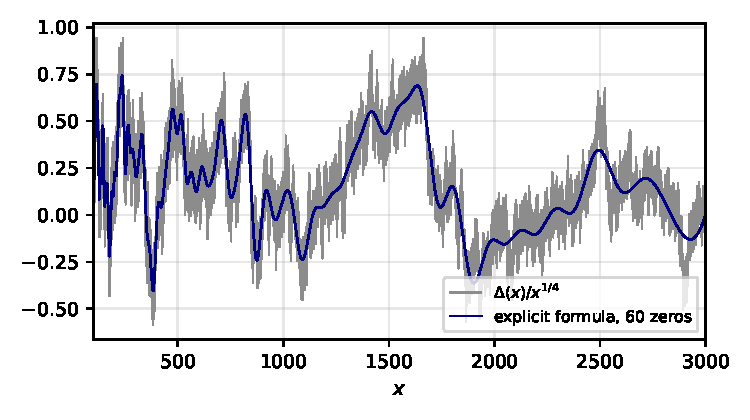
\includegraphics[width=0.8\textwidth]{fig/sqfree_atoms.pdf}
\caption{The normalised error $\Delta(x)/x^{1/4}$ of the squarefree count on $[100,3000]$ (grey) and the explicit formula \eqref{eq:sqfree:explicit} with the first $60$ zeros and the trivial terms at $s=-1$, $-3$ and $-5$, divided by $x^{1/4}$ (dark). Drawn by \texttt{sqfree\_atoms.py}.}
\label{fig:sqfree:atoms}
\end{figure}

For the sum $\sum_{n\le x}\mu(n)^2/n$ of Proposition~\ref{prop:sqfree:alpha1} the same atoms appear at $s=\rho/2-1$, with residues $\zeta(\rho/2)x^{\rho/2-1}/((\rho-2)\zeta'(\rho))$ of size $x^{-3/4}$ under RH (of modulus $0.09991\,x^{-3/4}$ for the first zero), inside the error $O(x^{-1/2})$. Likewise the error $\mathcal E_\alpha$ of \eqref{eq:sqfree:alpha}, for $\frac12<\alpha<1$, has atoms of size $x^{1/4-\alpha}$. By \eqref{eq:sqfree:Ealpha}, a pointwise bound of that order in either case would follow from $\Delta(x)=O(x^{1/4+\varepsilon})$, and it is open for the same reason.

\subsection{Smoothed counts}\label{sec:sqfree:smooth}

Smoothing the count removes the obstacle. For $x>0$ let
\[
Q_1(x)=\sum_{n\ge1}\mu(n)^2e^{-n/x}=\sum_{d\ge1}\frac{\mu(d)}{e^{d^2/x}-1},\qquad Q_2(x)=\sum_{n\ge1}\mu(n)^2\Big(1+\frac{2n}x\Big)e^{-2n/x},
\]
the second form of $Q_1$ by $\mu(n)^2=\sum_{d^2\mid n}\mu(d)$. If $G_{1,x}$ is exponential and $G_{2,x}$ has the Gamma(2) law, both with mean $x$, then $P(G_{1,x}\ge n)=e^{-n/x}$ and $P(G_{2,x}\ge n)=(1+2n/x)e^{-2n/x}$, so $Q_1(x)=\E Q(G_{1,x})$ and $Q_2(x)=\E Q(G_{2,x})$. Since $\int_0^\infty e^{-n/x}x^{-s-1}dx=\Gamma(s)n^{-s}$ and $\int_0^\infty(1+2n/x)e^{-2n/x}x^{-s-1}dx=(1+s)\Gamma(s)(2n)^{-s}$, the Mellin transforms are
\begin{equation}\label{eq:sqfree:mellin12}
\begin{aligned}
\int_0^\infty Q_1(x)\,x^{-s-1}dx&=\Gamma(s)D(s),\\
\int_0^\infty Q_2(x)\,x^{-s-1}dx&=(1+s)\Gamma(s)\,2^{-s}D(s),\qquad\re s>1 .
\end{aligned}
\end{equation}
The kernels $\Gamma(s)$ and $(1+s)\Gamma(s)2^{-s}$ have no zeros in $\re s>0$ and decay exponentially on vertical lines.

\begin{lemma}\label{lem:sqfree:descent}
If $D(s)=\zeta(s)/\zeta(2s)$ is analytic in the half plane $\re s>\frac14$ apart from $s=1$, then RH holds.
\end{lemma}

\begin{proof}
Let $\rho$ be a zero with $\beta=\re\rho>\frac12$. Then $\re(\rho/2)>\frac14$, so the pole of $1/\zeta(2s)$ at $s=\rho/2$ must be cancelled, that is $\zeta(\rho/2)=0$. Since $\frac14<\re(\rho/2)<\frac12$, the functional equation and the reflection $s\mapsto\bar s$ make $\rho'=1-\bar\rho/2$ a zero, with $\re\rho'=1-\beta/2>\frac12$ and $\im\rho'=\im\rho/2$. Iterating gives zeros $\rho_j$ whose real parts tend to $\frac23$, the fixed point of $\beta\mapsto1-\beta/2$, and whose imaginary parts are $\im\rho/2^j$. Since $\zeta<0$ on $(0,1)$, $\im\rho\ne0$, so the $\rho_j$ are distinct and accumulate at $\frac23$, where $\zeta$ is analytic and not identically zero, a contradiction.
\end{proof}

\begin{theorem}\label{thm:sqfree:smooth}
\textup{(i)} RH holds if and only if $Q_1(x)=\frac6{\pi^2}x+O(x^{1/4+\varepsilon})$ for every $\varepsilon>0$, and if and only if $Q_2(x)=\frac6{\pi^2}x+O(x^{1/4+\varepsilon})$ for every $\varepsilon>0$.

\textup{(ii)} Under RH, if the zeros are simple, then
\begin{align*}
Q_1(x)&=\frac6{\pi^2}x+1+\sum_\rho A_\rho\,x^{\rho/2}+\frac{c_1\log x+c_2}x+O(x^{-2}),\\
Q_2(x)&=\frac6{\pi^2}x+1+\sum_\rho B_\rho\,x^{\rho/2}+\frac{2c_1}x+O(x^{-2}),\\
A_\rho&=\frac{\Gamma(\rho/2)\,\zeta(\rho/2)}{2\zeta'(\rho)},\qquad B_\rho=\Big(1+\frac\rho2\Big)\frac{2^{-\rho/2}\,\Gamma(\rho/2)\,\zeta(\rho/2)}{2\zeta'(\rho)},
\end{align*}
the sums over $\rho$ taken over $|\im\rho|<2T_j$ along a sequence $T_j\to\infty$, with
\begin{align*}
c_1&=-\frac{\zeta(-1)}{2\zeta'(-2)}=-1.36843277762021,\\
c_2&=c_1\Big(1-\gamma_E+\frac{\zeta'(-1)}{\zeta(-1)}-\frac{\zeta''(-2)}{\zeta'(-2)}\Big)=-0.339381226129599 .
\end{align*}
\end{theorem}

\begin{proof}
(i) Suppose RH. By Section~14.2 of \cite{Titchmarsh}, $1/\zeta(\sigma+it)=O(|t|^\varepsilon)$ uniformly for $\sigma\ge\frac12+\varepsilon$, and $\zeta(\sigma+it)$ grows at most polynomially in $|t|$ on vertical strips, while $\Gamma(s)$ decays exponentially. Move the line of integration in $Q_1(x)=\frac1{2\pi i}\int_{(2)}\Gamma(s)D(s)x^s\,ds$ to $\re s=\frac14+\varepsilon$. The only pole crossed is $s=1$, with residue $\Gamma(1)/\zeta(2)\cdot x=6x/\pi^2$; the point $s=\frac12$ is regular because $\zeta(2s)$ has a pole there. On the new line $|\Gamma(s)D(s)|$ is integrable and the integral is $O(x^{1/4+\varepsilon})$. The same argument with the kernel $(1+s)\Gamma(s)2^{-s}$ treats $Q_2$.

Conversely, suppose $Q_1(x)=\frac6{\pi^2}x+O(x^{1/4+\varepsilon})$ for every $\varepsilon>0$. For $\re s>1$, by \eqref{eq:sqfree:mellin12},
\[
\Gamma(s)D(s)-\frac6{\pi^2}\,\frac1{s-1}=\int_1^\infty\Big(Q_1(x)-\frac6{\pi^2}x\Big)x^{-s-1}dx+\int_0^1Q_1(x)\,x^{-s-1}dx .
\]
The first integral converges and is analytic in $\re s>\frac14$, by the hypothesis, and the second is entire, since $Q_1(x)=O(e^{-1/x})$ as $x\to0$. As $\Gamma$ has no zeros, $D$ is analytic in $\re s>\frac14$ apart from $s=1$, and Lemma~\ref{lem:sqfree:descent} gives RH. The same argument applies to $Q_2$.

(ii) By Theorem~9.7 of \cite{Titchmarsh} there are heights $T_j\in[j,j+1]$ at which $1/\zeta(\sigma\pm2iT_j)=T_j^{O(1)}$ uniformly for $-1\le\sigma\le2$, and on the left of the line $\re s=-\frac12$ the functional equation bounds $1/\zeta(2s)$ polynomially. Move the line of integration to $\re s=-\frac52$ along the rectangles of height $T_j$; the exponential decay of $\Gamma$ makes the horizontal sides vanish as $j\to\infty$, and the integral on the new line is $O(x^{-5/2})$. The poles crossed are $s=1$; the points $\rho/2$, with the residues $A_\rho x^{\rho/2}$ and $B_\rho x^{\rho/2}$; $s=0$, where $\Gamma(s)D(s)$ and $(1+s)\Gamma(s)2^{-s}D(s)$ have residue $D(0)=\zeta(0)/\zeta(0)=1$; $s=-1$; and $s=-2$, a simple pole of both, which gives a multiple of $x^{-2}$. At $s=-1$, $\Gamma$ has a simple pole and $1/\zeta(2s)$ another, from the trivial zero $-2$ of $\zeta$, so $\Gamma(s)D(s)=c_1(s+1)^{-2}+c_2(s+1)^{-1}+O(1)$, with $c_1$ and $c_2$ from the expansions $\Gamma(s)=-(s+1)^{-1}(1+(1-\gamma_E)(s+1)+\cdots)$, $\zeta(s)=\zeta(-1)(1+\frac{\zeta'(-1)}{\zeta(-1)}(s+1)+\cdots)$ and $\zeta(2s)=2\zeta'(-2)(s+1)(1+\frac{\zeta''(-2)}{\zeta'(-2)}(s+1)+\cdots)$, and the residue of $\Gamma(s)D(s)x^s$ is $x^{-1}(c_1\log x+c_2)$. The factor $1+s$ makes the pole of $(1+s)\Gamma(s)2^{-s}D(s)$ at $s=-1$ simple, with residue $2c_1$ times $x^{-1}$.
\end{proof}

At the even negative integers $\Gamma(s)D(s)$ has simple poles, since $\zeta(s)$ vanishes there together with $\zeta(2s)$, and at the odd ones double poles: \texttt{sqfree\_smooth.py} computes the Laurent coefficients at $s=-1,\dots,-6$ by the trapezoid rule on circles of radius $0.3$ and reproduces the closed forms of $c_1$ and $c_2$ within $5\times10^{-46}$. For $Q_2$ the double pole at $s=-1$ becomes a simple one, with residue $2c_1$.

The coefficients $A_\rho$ are tiny, $|A_{\rho_1}|=1.648\times10^{-5}$ and $6.29\times10^{-82}$ at the hundredth zero, because $|\Gamma(\rho/2)|$ decays like $e^{-\pi\gamma/4}$. \texttt{sqfree\_smooth.py} checks part~(ii) for $Q_1$: the smoothed error is the sum of the atom terms and the trivial terms to the working precision. Table~\ref{tab:sqfree:gamma2} in Section~\ref{sec:sqfree:mertens} does the same for $Q_2$.

The Perron kernel $x^s/s$ decays only like $1/|t|$, so the atom series for $Q(x)$ has no exponential damping, and bounding its partial sums would need control of $\sum_{|\gamma|\le T}|\zeta(\rho/2)/(\rho\zeta'(\rho))|$, which is out of reach.

\subsection{Mean square, and how much smoothing the sharp count needs}\label{sec:sqfree:meansq}

Two further results bracket the sharp problem. The first settles it on average; it is presumably folklore. For $\re s>1$ let
\[
F(s)=\int_1^\infty\Delta(x)\,x^{-s-1}dx=\frac{D(s)}s-\frac6{\pi^2}\,\frac1{s-1},
\]
the second form because $\int_1^\infty Q(x)x^{-s-1}dx=D(s)/s$.

\begin{theorem}\label{thm:sqfree:meansq}
RH holds if and only if $\int_X^{2X}\Delta(x)^2\,dx=O(X^{3/2+\varepsilon})$ for every $\varepsilon>0$, that is, if and only if the root mean square of $\Delta$ on every range $[X,2X]$ is $O(X^{1/4+\varepsilon})$.
\end{theorem}

\begin{proof}
Suppose RH. Then $F$ continues analytically to $\re s>\frac14$: the poles of $D$ at the points $\rho/2$ lie on the line $\re s=\frac14$, $s=\frac12$ is regular, and the pole at $s=1$ cancels. By Section~14.2 of \cite{Titchmarsh}, under RH $\zeta(\sigma+it)=O(|t|^{\max(0,\frac12-\sigma)+\varepsilon})$ and $1/\zeta(2\sigma+2it)=O(|t|^\varepsilon)$ uniformly for $\sigma\ge\frac14+\varepsilon$ and $|t|\ge1$, so $F(\sigma+it)=O(|t|^{-3/4+2\varepsilon})$ uniformly there. For $w>2$ let $I(w)=\int_1^\infty\Delta(x)^2x^{-w-1}dx$, the Laplace transform in $v=\log x$ of the nonnegative function $\Delta(e^v)^2$. Plancherel's theorem for the function $v\mapsto\Delta(e^v)e^{-wv/2}$ on $(0,\infty)$, whose Fourier transform is $t\mapsto F(\frac w2+it)$, and the symmetry $F(\bar s)=\overline{F(s)}$ give
\[
I(w)=\frac1{2\pi}\int_{-\infty}^\infty F\Big(\frac w2+it\Big)\,F\Big(\frac w2-it\Big)\,dt,\qquad w>2 .
\]
The right side is analytic in $w$ on $\re w>\frac12$, since the integrand is analytic there and $O(|t|^{-3/2+4\varepsilon})$ locally uniformly. So $I$, the Laplace transform of a nonnegative function, continues analytically to a neighbourhood of every point of $(\frac12,\infty)$, and Landau's theorem \cite[Chapter~II, Theorem~5b]{Widder41} puts its abscissa of convergence at or below $\frac12$. Hence $I(w)<\infty$ for every $w>\frac12$, and $\int_X^{2X}\Delta^2\,dx\le(2X)^{w+1}I(w)=O(X^{3/2+\varepsilon})$ with $w=\frac12+\varepsilon$.

Conversely, by the Cauchy Schwarz inequality the hypothesis gives $\int_X^{2X}|\Delta(x)|x^{-\sigma-1}dx=O(X^{1/4+\varepsilon-\sigma})$, so, summing over $X=2^j$, the integral defining $F$ converges absolutely for $\re s>\frac14$. Then $D(s)=s\big(F(s)+\frac6{\pi^2}\frac1{s-1}\big)$ is analytic in $\re s>\frac14$ apart from $s=1$, and Lemma~\ref{lem:sqfree:descent} gives RH.
\end{proof}

Table~\ref{tab:sqfree:rms} gives the root mean square of $\Delta$ on dyadic ranges, computed exactly from the sieve: on $[n,n+1)$ the error decreases linearly from $\Delta_n=Q(n)-6n/\pi^2$ to $\Delta_n-6/\pi^2$, so $\int_n^{n+1}\Delta^2=\Delta_n^2-\frac6{\pi^2}\Delta_n+\frac{12}{\pi^4}$, and the extremes over real $x$ are taken at integers or as left limits there. Over the eighteen ranges $[X,2X]$ with $X=10^4\cdot2^j$, $j=0,\dots,13$, and $X=10^4,\dots,10^8$, the root mean square divided by $X^{1/4}$ lies between $0.2337$ and $0.3606$ and the largest $|\Delta(x)|/X^{1/4}$ between $0.6851$ and $1.0361$; on $[10^3,2\times10^8]$ the largest value of $\Delta(x)/x^{1/4}$ is $0.9807$, near $x=47523$, and the least $-0.8685$, near $x=80157$.

\begin{table}[htbp]
\centering\small
\begin{tabular}{rccc}
\toprule
$X$ & $\big(\frac1X\int_X^{2X}\Delta^2\big)^{1/2}\big/X^{1/4}$ & $\max_{[X,2X]}|\Delta(x)|/X^{1/4}$ & near $x=$\\
\midrule
$10^4$ & $0.2701$ & $0.8979$ & $18471$\\
$10^5$ & $0.2494$ & $0.6851$ & $128599$\\
$10^6$ & $0.2779$ & $0.8382$ & $1618611$\\
$10^7$ & $0.3541$ & $0.9931$ & $17199381$\\
$10^8$ & $0.2812$ & $0.8636$ & $144151023$\\
\bottomrule
\end{tabular}
\caption{Root mean square and largest absolute value of the squarefree error $\Delta$ on the ranges $[X,2X]$, divided by $X^{1/4}$, over real $x$; the largest value on $[10^7,2\times10^7]$ is the left limit at $17199381$, and over the integers alone it is $0.982$. Computed by \texttt{sqfree\_sieve.py}.}
\label{tab:sqfree:rms}
\end{table}

\begin{corollary}\label{cor:sqfree:omega}
\textup{(i)} Under RH, for every $\varepsilon>0$ the set of $x\in[X,2X]$ with $|\Delta(x)|>X^{1/4+\varepsilon}$ has measure $O(X^{1-\varepsilon})$.

\textup{(ii)} With no hypothesis,
\[
\limsup_{x\to\infty}\frac{\Delta(x)}{x^{1/4}}\ge|R_{\rho_1}|,\qquad\liminf_{x\to\infty}\frac{\Delta(x)}{x^{1/4}}\le-|R_{\rho_1}|,
\]
where $R_{\rho_1}=\zeta(\rho_1/2)/(\rho_1\zeta'(\rho_1))$ and $|R_{\rho_1}|=0.100404$. The same holds for $Q_2(x)-\frac6{\pi^2}x-1$ with $|B_{\rho_1}|=9.944\times10^{-5}$ in place of $|R_{\rho_1}|$.
\end{corollary}

\begin{proof}
(i) is Chebyshev's inequality applied to Theorem~\ref{thm:sqfree:meansq}. For (ii) suppose that $\Delta(x)\le c\,x^{1/4}$ for $x\ge x_0$, with $0<c<|R_{\rho_1}|$. The function $L(s)=\int_{x_0}^\infty(cx^{1/4}-\Delta(x))x^{-s-1}dx$ is the Laplace transform in $\log x$ of a nonnegative function, and for $\re s>1$
\[
L(s)=\frac{c\,x_0^{1/4-s}}{s-\frac14}-F(s)+E(s),
\]
with $E$ entire. The right side has no singularity on the real half line $(\frac14,\infty)$: a real pole of $D$ there would be a real zero of $\zeta$ in $(\frac12,\infty)$, of which there are none, $s=\frac12$ is regular, and the pole at $s=1$ cancels. By Landau's theorem the integral $L(s)$ converges for $\re s>\frac14$, so $F$ is analytic there (which already gives RH, by Lemma~\ref{lem:sqfree:descent}), and $|L(\sigma+it)|\le L(\sigma)$ for $\sigma>\frac14$. As $\sigma\downarrow\frac14$, $L(\sigma)=c/(\sigma-\frac14)+O(1)$, since $F$ is analytic at $s=\frac14$, where $\zeta(2s)=\zeta(\frac12)\ne0$. At $s=\sigma+\frac i2\gamma_1$ the first and last terms of the display are $O(1)$, while $F(s)=R_{\rho_1}/(\sigma-\frac14)+O(1)$, because $D(s)/s$ has a simple pole at $\rho_1/2$ with residue $R_{\rho_1}$ (the zero $\rho_1$ is simple and $\zeta(\rho_1/2)\ne0$). Hence $|R_{\rho_1}|\le c$, a contradiction. The lower bound is the same argument applied to $c\,x^{1/4}+\Delta(x)$, and the smoothed case is the same argument with the kernel $(1+s)\Gamma(s)2^{-s}$, whose residue at $\rho_1/2$ is $B_{\rho_1}$.
\end{proof}



The second result measures the cost of sharpening. Let $G_{n,x}$ have the Gamma($n$) law with mean $x$, so that $G_{n,x}$ concentrates at $x$ in a window of width $x/\sqrt n$; $Q_1(x)=\E Q(G_{1,x})$ and $Q_2(x)=\E Q(G_{2,x})$.

\begin{proposition}\label{prop:sqfree:gamman}
Under RH, uniformly in $n\ge1$,
\[
\E Q(G_{n,x})=\frac6{\pi^2}\,x+O_\varepsilon\big(x^{1/4+\varepsilon}\,n^{1/8+\varepsilon}\big).
\]
\end{proposition}

\begin{proof}
With rate $\lambda=n/x$, $P(G_{n,x}\ge m)=\Gamma(n,\lambda m)/\Gamma(n)$, whose Mellin transform in $\lambda m$ is $\Gamma(s+n)/(s\Gamma(n))$, so $\E Q(G_{n,x})=\frac1{2\pi i}\int_{(2)}D(s)\frac{\Gamma(s+n)}{s\Gamma(n)}\big(\frac xn\big)^sds$. Move the line to $\re s=c=\frac14+\varepsilon$, collecting $6x/\pi^2$ at $s=1$. On the new line $|\Gamma(n+c+it)|/\Gamma(n)=O\big(n^c\exp(-\kappa\min(t^2/n,|t|))\big)$ for an absolute $\kappa>0$, since $\Gamma(n+c)/\Gamma(n)=O(n^c)$ and $|\Gamma(n+c+it)/\Gamma(n+c)|^2=\prod_{k\ge0}\big(1+t^2/(n+c+k)^2\big)^{-1}$; the factors with $k<n$ give $e^{-\kappa t^2/n}$ when $|t|\le n$, and those with $k\le|t|$ give $e^{-\kappa|t|}$ when $|t|>n$. Under RH, $|D(c+it)|=O(|t|^{1/4+\varepsilon})$ for $|t|\ge1$ (Section~14.2 of \cite{Titchmarsh} and the functional equation). The remaining integral is therefore $O\big(x^c\int(1+|t|)^{-3/4+\varepsilon}e^{-\kappa\min(t^2/n,|t|)}dt\big)=O(x^cn^{1/8+\varepsilon})$, the integral being dominated by $|t|\lesssim\sqrt n$.
\end{proof}

Balancing the window against the loss gives a bound for the sharp count.

\begin{corollary}\label{cor:sqfree:twofifths}
Under RH, $\Delta(x)=O(x^{2/5+\varepsilon})$ for every $\varepsilon>0$.
\end{corollary}

\begin{proof}
Since $Q$ is nondecreasing and counts integers, $|Q(y)-Q(x)|\le|y-x|+1$, so $|\E Q(G_{n,x})-Q(x)|\le\E|G_{n,x}-x|+1\le x/\sqrt n+1$. With Proposition~\ref{prop:sqfree:gamman}, $\Delta(x)=O(x^{1/4+\varepsilon}n^{1/8+\varepsilon}+x/\sqrt n)$, and $n=\lceil x^{6/5}\rceil$ balances the two terms at $x^{2/5+O(\varepsilon)}$.
\end{proof}

The exponent $\frac25$ is weaker than the known conditional exponents. If the loss $n^{1/8}$ were replaced by $n^\delta$, the same balance would give $\Delta(x)=O(x^{1-3/(8\delta+4)+\varepsilon})$, which tends to $x^{1/4+\varepsilon}$ as $\delta\to0$; conversely $\Delta(x)=O(x^{1/4+\varepsilon})$ gives $|\E Q(G_{n,x})-\frac6{\pi^2}x|\le\E|\Delta(G_{n,x})|=O(x^{1/4+\varepsilon})$ uniformly in $n$, by Jensen's inequality. So the sharp conjecture amounts to removing the loss, which needs cancellation in $\int_{|t|\le T}D(\frac14+it)x^{it}\,dt/t$ and not only a bound on the size of the integrand.

\subsection{Gamma(2) smoothing and the Mertens function}\label{sec:sqfree:mertens}

The elementary method rests on the terms $\mu(d)(\lfloor x/d^2\rfloor-x/d^2)=-\mu(d)\{x/d^2\}$ of \eqref{eq:sqfree:Qd}. Following the idea of Steutel and Thiemann of splitting a random variable into its integer and fractional parts \cite{SteutelThiemann89}, we randomise $x$ by a gamma law. Theorem~\ref{thm:sqfree:threshold} shows that here shape two is the largest for which the average is taken under a positive law.

Let $Y$ have the Gamma($\nu$) law with rate $\lambda$, let $a>0$ and $y=\lambda a$. Then $\E\lfloor Y/a\rfloor=\sum_{m\ge1}P(Y\ge ma)=\sum_{m\ge1}\Gamma(\nu,my)/\Gamma(\nu)$ and $\E Y/a=\nu/y$, so the expected fractional part is
\[
\E\{Y/a\}=g_\nu(y)=\frac\nu y-\sum_{m\ge1}\frac{\Gamma(\nu,my)}{\Gamma(\nu)} .
\]
For $\nu=1$, Steutel and Thiemann observed that $\lfloor Y/a\rfloor$ is geometric and $\{Y/a\}$ an independent truncated exponential variable, with $\E\lfloor Y/a\rfloor=1/(e^y-1)$ and $g_1(y)=1/y-1/(e^y-1)$.

\begin{lemma}\label{lem:sqfree:frac2}
For $\nu=2$,
\[
\E\lfloor Y/a\rfloor=\frac1{e^y-1}+\frac y{4\sinh^2(y/2)},\qquad g_2(y)=\frac2y-\frac1{e^y-1}-\frac y{4\sinh^2(y/2)} .
\]
For $0<|y|<2\pi$, with the Bernoulli numbers $B_{2k}$,
\[
g_2(y)=\frac12+\sum_{k\ge2}\frac{(2k-2)B_{2k}}{(2k)!}\,y^{2k-1}=\frac12-\frac{y^3}{360}+\frac{y^5}{7560}-\cdots,
\]
$g_2(y)=2/y+O(ye^{-y})$ as $y\to\infty$, and for every $\nu>0$
\[
\int_0^\infty g_\nu(y)\,y^{s-1}\,dy=-\frac{\Gamma(s+\nu)\,\zeta(s)}{s\,\Gamma(\nu)},\qquad 0<\re s<1,
\]
which is $-(1+s)\Gamma(s)\zeta(s)$ for $\nu=2$.
\end{lemma}

\begin{proof}
For $\nu=2$, $P(Y\ge ma)=(1+my)e^{-my}$, and $\sum_me^{-my}=1/(e^y-1)$, $\sum_mmye^{-my}=y/(4\sinh^2(y/2))$. For the expansion use $1/(e^y-1)=1/y-\frac12+\sum_{k\ge1}B_{2k}y^{2k-1}/(2k)!$ and $y/(4\sinh^2(y/2))=-y\frac d{dy}(e^y-1)^{-1}$. For the Mellin transform write $g_\nu(y)=\E\{Y/y\}$ with $Y$ of law Gamma($\nu$,1), substitute $u=Y/y$, and use the classical formula $\int_0^\infty\{u\}u^{-s-1}du=-\zeta(s)/s$ for $0<\re s<1$ \cite[Section~2.1]{Titchmarsh}: the transform is $\E Y^s\cdot(-\zeta(s)/s)$, with $\E Y^s=\Gamma(s+\nu)/\Gamma(\nu)$.
\end{proof}

The terms of the elementary method now read $\E\big[\mu(d)\big(\lfloor G_{2,x}/d^2\rfloor-G_{2,x}/d^2\big)\big]=-\mu(d)g_2(2d^2/x)$ for $G_{2,x}$ of the Gamma(2) law with mean $x$, and since $0\le g_2(y)\le\min(1,2/y)$ the sum over all $d$ converges absolutely, with no truncation at $d^2\le x$:
\begin{equation}\label{eq:sqfree:EQ}
Q_2(x)=\sum_{n\ge1}\mu(n)^2\Big(1+\frac{2n}x\Big)e^{-2n/x}=\frac6{\pi^2}\,x-\sum_{d\ge1}\mu(d)\,g_2\Big(\frac{2d^2}x\Big).
\end{equation}

\begin{theorem}\label{thm:sqfree:mertens}
Let
\[
f_2(y)=-2g_2'(y)=\frac4{y^2}-\frac{y\cosh(y/2)}{2\sinh^3(y/2)},\qquad y>0 .
\]
Then $f_2>0$, $f_2(y)=y^2/60+O(y^4)$ as $y\to0$ and $f_2(y)\sim4/y^2$ as $y\to\infty$, and $f_2$ is the density of a probability law $\mathcal V_2$ with $P(\mathcal V_2\ge y)=2g_2(y)$ and
\[
\E\mathcal V_2^s=-2\,\Gamma(s+2)\,\zeta(s),\qquad -3<\re s<1 .
\]
For every $x>0$,
\[
Q_2(x)=\frac6{\pi^2}\,x-\frac12\,\E M\Big(\sqrt{x\mathcal V_2/2}\Big).
\]
Moreover $f_2$ is twice the difference between the continuous and the integer mixtures of the Gamma(2) densities $\gamma_{2,\lambda}(y)=\lambda^2ye^{-\lambda y}$ over their rate:
\[
f_2(y)=2\Big(\int_0^\infty\gamma_{2,\lambda}(y)\,d\lambda-\sum_{m\ge1}\gamma_{2,m}(y)\Big)=-2\int_0^\infty\Big(\{\lambda\}-\frac12\Big)\,\partial_\lambda\gamma_{2,\lambda}(y)\,d\lambda .
\]
\end{theorem}

\begin{proof}
With $z=y/2$, $f_2(y)>0$ is $(\sinh z/z)^3>\cosh z$, Lazarevi\'c's inequality \cite{Lazarevic66}. The expansion at $0$ follows from Lemma~\ref{lem:sqfree:frac2}. The mass is $2(g_2(0+)-g_2(\infty))=1$ and the tail is $2g_2(y)$. Integrating by parts in the Mellin formula of Lemma~\ref{lem:sqfree:frac2} gives $\E\mathcal V_2^s=2s\int_0^\infty y^{s-1}g_2(y)\,dy=-2s(1+s)\Gamma(s)\zeta(s)$ for $0<\re s<1$, and the behaviour at $0$ and at infinity extends the integral and the identity to $-3<\re s<1$. For the representation, $P(\sqrt{x\mathcal V_2/2}\ge d)=P(\mathcal V_2\ge2d^2/x)=2g_2(2d^2/x)$, so $\frac12\E M(\sqrt{x\mathcal V_2/2})=\sum_d\mu(d)g_2(2d^2/x)$, the interchange being justified by absolute convergence, and \eqref{eq:sqfree:EQ} gives the formula. Finally $\int_0^\infty\gamma_{2,\lambda}(y)\,d\lambda=2/y^2$ and $\sum_m\gamma_{2,m}(y)=y\sum_mm^2e^{-my}=y\cosh(y/2)/(4\sinh^3(y/2))$, and the last form is the Euler Maclaurin formula $\int_0^\infty h-\sum_{m\ge1}h(m)=-\int_0^\infty(\{\lambda\}-\frac12)h'(\lambda)\,d\lambda$ for $h=\gamma_{2,\cdot}(y)$, which vanishes at $\lambda=0$.
\end{proof}

The exponential case is the same with
\[
f_1(y)=-2g_1'(y)=\frac2{y^2}-\frac1{2\sinh^2(y/2)}=2\Big(\int_0^\infty\lambda e^{-\lambda y}d\lambda-\sum_{m\ge1}me^{-my}\Big)>0,
\]
positive because $\sinh z>z$, with $f_1(0+)=\frac16$, $\E\mathcal V_1^s=-2\Gamma(s+1)\zeta(s)$ for $-1<\re s<1$, and
\[
Q_1(x)=\frac6{\pi^2}\,x-\frac12\,\E M\Big(\sqrt{x\mathcal V_1}\Big).
\]

\begin{corollary}\label{cor:sqfree:mertens}
\textup{(i)} With no hypothesis, $Q_\nu(x)=\frac6{\pi^2}x+o(x^{1/2})$ for $\nu=1,2$. \textup{(ii)} Under RH, $|Q_2(x)-\frac6{\pi^2}x|\le\frac12\E|M(\sqrt{x\mathcal V_2/2})|=O(x^{1/4+\varepsilon})$, and likewise for $Q_1$; this is a second proof of the forward half of Theorem~\ref{thm:sqfree:smooth}(i).
\end{corollary}

\begin{proof}
(i) $|M(t)|\le t$ and $M(t)=o(t)$, and $\E\mathcal V_\nu^{1/2}<\infty$, so dominated convergence gives $\E M(\sqrt{x\mathcal V_2/2})=o(x^{1/2})$, and likewise for $\mathcal V_1$. (ii) RH gives $M(t)=O(t^{1/2+\varepsilon})$ \cite[Section~14.25]{Titchmarsh}, and $\E\mathcal V_\nu^{1/4+\varepsilon}<\infty$.
\end{proof}

Table~\ref{tab:sqfree:gamma2} checks \eqref{eq:sqfree:EQ} and Theorem~\ref{thm:sqfree:smooth}(ii) for $Q_2$. It computes $Q_2(x)=\sum_d\mu(d)\,\E\lfloor G_{2,x}/d^2\rfloor=\sum_d\mu(d)\big(1/(e^t-1)+t/(4\sinh^2(t/2))\big)$, $t=2d^2/x$, whose terms with $t>140$ are below $10^{-55}$, and this agrees with the direct sum over $n$, in double precision, within $10^{-10}$ up to $x=10^6$. The sum \eqref{eq:sqfree:EQ} truncated at $d\le2\times10^5$, as in the first author's note, loses $2.2\times10^{-4}$ at $x=10^6$, because $g_2(2d^2/x)$ is close to $x/d^2$ for large $d$ and the tail $x\sum_{d>2\times10^5}\mu(d)/d^2$ is left out.

\begin{table}[htbp]
\centering\footnotesize
\setlength{\tabcolsep}{3.5pt}
\fitwidth{\begin{tabular}{rcccccc}
\toprule
$x$ & $Q_2(x)-\frac6{\pi^2}x$ & $d\le2\cdot10^5$ & $\frac{Q_2(x)-\frac6{\pi^2}x-1}{x^{1/4}}$ & $100$ atoms & trivial terms & residual\\
\midrule
$10^3$ & $0.997161220898$ & $0.997161002208$ & $-5.048\times10^{-4}$ & $-1.0571\times10^{-4}$ & $-2.73307\times10^{-3}$ & $-1.0\times10^{-23}$\\
$10^4$ & $1.00094524529$ & $1.00094305839$ & $9.452\times10^{-5}$ & $1.21889\times10^{-3}$ & $-2.73648\times10^{-4}$ & $-1.3\times10^{-30}$\\
$10^5$ & $0.996620193442$ & $0.99659832449$ & $-1.9006\times10^{-4}$ & $-3.35244\times10^{-3}$ & $-2.73683\times10^{-5}$ & $-1.5\times10^{-37}$\\
$10^6$ & $1.00610290943$ & $1.00588421991$ & $1.9299\times10^{-4}$ & $6.10565\times10^{-3}$ & $-2.73686\times10^{-6}$ & $-1.8\times10^{-41}$\\
$10^7$ & $0.992114718377$ & & $-1.4022\times10^{-4}$ & $-7.88501\times10^{-3}$ & $-2.73687\times10^{-7}$ & $-3.9\times10^{-42}$\\
$10^8$ & $1.00440085379$ & & $4.4009\times10^{-5}$ & $4.40088\times10^{-3}$ & $-2.73687\times10^{-8}$ & $-2.2\times10^{-38}$\\
\bottomrule
\end{tabular}}
\caption{The Gamma(2) smoothed count: $Q_2(x)-6x/\pi^2$, the sum \eqref{eq:sqfree:EQ} truncated at $d\le2\times10^5$, the normalised error, the contribution $2\re\sum_{k\le100}B_{\rho_k}x^{\rho_k/2}$ of the first hundred atoms, the residues at $s=-1,\dots,-6$, whose leading part is $2c_1/x$, and the residual. The constant $1$ is the residue $D(0)$ at $s=0$. Computed by \texttt{sqfree\_smooth.py} at $45$ digits.}
\label{tab:sqfree:gamma2}
\end{table}

\subsection{Gamma shapes: two is the threshold}\label{sec:sqfree:shape}

For every real shape $\nu>0$, $f_\nu=-2g_\nu'$ is a signed density of total mass $2g_\nu(0+)=1$, and the argument of Theorem~\ref{thm:sqfree:mertens} gives, for $Y$ of the Gamma($\nu$) law with rate $\lambda$,
\begin{gather*}
\E Q(Y)=\frac6{\pi^2}\,\E Y-\frac12\int_0^\infty M\Big(\sqrt{y/\lambda}\Big)f_\nu(y)\,dy,\\
\int_0^\infty y^sf_\nu(y)\,dy=-\frac{2\,\Gamma(s+\nu)\,\zeta(s)}{\Gamma(\nu)},\qquad -\nu<\re s<1 .
\end{gather*}


Write $\gamma_a(t)=t^{a-1}e^{-t}/\Gamma(a)$ for the Gamma($a$) density, and let
\begin{gather*}
\mathcal R_\nu(y)=y\sum_{m\ge1}\gamma_{\nu+1}(my)=\frac{y^{\nu+1}}{\Gamma(\nu+1)}\sum_{m\ge1}m^\nu e^{-my},\\
q_\nu(y)=\frac{\Gamma(\nu+1)\,\big(1-\mathcal R_\nu(y)\big)}{y^{\nu+1}},
\end{gather*}
so that $\mathcal R_\nu(y)$ is the right Riemann sum with step $y$ of the Gamma($\nu+1$) density, whose integral is $1$.

\begin{lemma}\label{lem:sqfree:riemann}
For $\nu>0$ and $y>0$,
\[
f_\nu(y)=\frac{2\nu\big(1-\mathcal R_\nu(y)\big)}{y^2}=\frac{2y^{\nu-1}}{\Gamma(\nu)}\,q_\nu(y),
\]
so $f_\nu\ge0$ exactly when $\mathcal R_\nu\le1$. For $0<y<2\pi$,
\[
q_\nu(y)=-\sum_{k\ge0}\zeta(-\nu-k)\,\frac{(-y)^k}{k!},
\]
and $\mathcal R_1(y)=(y/2)^2/\sinh^2(y/2)$, $\mathcal R_2(y)=(y/2)^3\cosh(y/2)/\sinh^3(y/2)$.
\end{lemma}

\begin{proof}
With $Y$ of the Gamma($\nu$,1) law and $c=1/y$, $g_\nu(y)=\E\{cY\}=c\nu-\sum_{m\ge1}P(Y\ge m/c)$, whose derivative in $c$ is $\nu-\sum_m(m/c^2)p_\nu(m/c)$, with $p_\nu=\gamma_\nu$ the density of $Y$. Since $tp_\nu(t)=\nu\gamma_{\nu+1}(t)$, the derivative is $\nu(1-\mathcal R_\nu(1/c))$, and returning to $y$ gives $g_\nu'(y)=-\nu(1-\mathcal R_\nu(y))/y^2$. The series is the expansion $\sum_mm^\nu e^{-my}=\Gamma(\nu+1)y^{-\nu-1}+\sum_{k\ge0}\zeta(-\nu-k)(-y)^k/k!$ of the polylogarithm, valid for $0<y<2\pi$.
\end{proof}

So $\mathcal R_1\le1$ is $\sinh z\ge z$ and $\mathcal R_2\le1$ is Lazarevi\'c's inequality. Near the origin $f_\nu$ has the sign of $q_\nu(0+)=-\zeta(-\nu)$, and at an even integer $\nu=2m$, where $\zeta(-2m)=0$, the sign of $q_{2m}(y)=\zeta(-2m-1)y+O(y^2)$. Since $\zeta$ is positive on $(-4,-2)$, $(-8,-6)$, \dots\ and $\zeta(-2m-1)=-B_{2m+2}/(2m+2)$, $f_\nu$ is negative near the origin exactly when $\nu\in(4j+2,4j+4]$ for some $j\ge0$.

\begin{theorem}\label{thm:sqfree:threshold}
$\{\nu>0:\ f_\nu\ge0\text{ on }(0,\infty)\}=(0,2]$. Thus two is the largest shape for which the gamma smoothed squarefree error is a positive average of the Mertens function, and the obstruction is the trivial zero of $\zeta$ at $-2$.
\end{theorem}

\begin{proof}
Let $\nu>2$ and suppose $f_\nu\ge0$. Since $f_\nu(y)\sim2\nu/y^2$ at infinity, $\int_1^\infty y^sf_\nu(y)\,dy$ converges and is analytic for $\re s<1$. The function $m(s)=-2\Gamma(s+\nu)\zeta(s)/\Gamma(\nu)$ is analytic in a neighbourhood of $(-\nu,1)$, so $\int_0^1y^sf_\nu(y)\,dy=m(s)-\int_1^\infty y^sf_\nu(y)\,dy$, a Laplace transform in $-\log y$ of a nonnegative function, continues analytically along the real interval $(-\nu,1)$. By Landau's theorem \cite[Chapter~II, Theorem~5b]{Widder41} it converges on all of $(-\nu,1)$, and there $m(s)=\int_0^\infty y^sf_\nu(y)\,dy>0$. But $\Gamma(s+\nu)>0$ on $(-\nu,1)$, while $\zeta(s)>0$ on $(-4,-2)$, which meets $(-\nu,1)$ because $\nu>2$, so $m(s)<0$ there, a contradiction.

Let $0<\nu\le2$. The cases $\nu=1$ and $\nu=2$ are the inequalities above. Otherwise write $\nu=k+\mu$ with $k\in\{0,1\}$ and $0<\mu<1$. Bernstein's formula $t^\mu=\frac\mu{\Gamma(1-\mu)}\int_0^\infty(1-e^{-st})s^{-\mu-1}ds$, applied to $t=mh$ in $\sum_m(mh)^{k+\mu}e^{-mh}$ and to $t$ in $\int_0^\infty t^{k+\mu}e^{-t}dt$, together with $h\sum_m(mh)^ke^{-mhc}=k!\,\mathcal R_k(hc)/c^{k+1}$ and $\int_0^\infty t^ke^{-ct}dt=k!/c^{k+1}$ for $c=1+s$, gives
\[
\Gamma(\nu+1)\big(\mathcal R_\nu(h)-1\big)=\frac{\mu\,h^{k+1}}{\Gamma(1-\mu)}\int_0^\infty\big(q_k(h(1+s))-q_k(h)\big)\,s^{-\mu-1}\,ds,\qquad h>0 .
\]
So $\mathcal R_\nu\le1$ follows if $q_k$ is nonincreasing. For $k=0$, $q_0(y)=1/y-1/(e^y-1)=g_1(y)$, which decreases because $f_1>0$. For $k=1$, $q_1(y)=1/y^2-1/(4\sinh^2(y/2))=f_1(y)/2$, and with $z=y/2$
\[
q_1'(y)=\frac14\Big(\frac{\cosh z}{\sinh^3z}-\frac1{z^3}\Big)<0
\]
by Lazarevi\'c's inequality.
\end{proof}

The script \texttt{sqfree\_gammanu.py} evaluates $1-\mathcal R_\nu$ for twenty shapes at $40$ digits, by the series of Lemma~\ref{lem:sqfree:riemann} for $y\le2.5$ and by the direct sum beyond, on $400$ geometrically spaced points in $[10^{-4},10^{0.4}]$ and $799$ equally spaced points in $(2.5,60]$. For the ten shapes $\nu=0.25,0.5,0.75,1,1.25,1.5,1.75,1.9,1.99,2$ no grid point gives a negative value; on the range $[0.02,15]$ the least values, from $2.68\times10^{-3}$ at $\nu=0.25$ to $6.90\times10^{-10}$ at $\nu=2$, are taken at its left end. Table~\ref{tab:sqfree:nu} shows the shapes above $2$: the negative set starts at the origin for the shapes in $(2,4]$ and in $(6,8]$, as the sign rule predicts.

\begin{table}[htbp]
\centering\footnotesize
\fitwidth{\begin{tabular}{rcccl}
\toprule
$\nu$ & $-\zeta(-\nu)$ & least value of $1-\mathcal R_\nu$ & at $y=$ & grid points with $1-\mathcal R_\nu<0$\\
\midrule
$2.01$ & $-3.012\times10^{-4}$ & $-7.310\times10^{-10}$ & $0.0273$ & from $10^{-4}$ to $0.0362$\\
$2.1$ & $-2.7295\times10^{-3}$ & $-4.941\times10^{-6}$ & $0.265$ & from $10^{-4}$ to $0.347$\\
$2.5$ & $-8.517\times10^{-3}$ & $-1.0763\times10^{-3}$ & $1.187$ & from $10^{-4}$ to $1.512$\\
$3$ & $-8.333\times10^{-3}$ & $-7.2304\times10^{-3}$ & $2.144$ & from $10^{-4}$ to $2.716$\\
$3.5$ & $-4.441\times10^{-3}$ & $-0.019006$ & $2.9745$ & from $10^{-4}$ to $3.723$\\
$4$ & $0$ & $-0.035249$ & $3.726$ & from $10^{-4}$ to $4.659$\\
$5$ & $3.968\times10^{-3}$ & $-0.076713$ & $5.084$ & from $1.716$ to $6.386$\\
$6$ & $0$ & $-0.12519$ & $6.323$ & from $3.076$ to $7.969$\\
$7$ & $-4.167\times10^{-3}$ & $-0.17715$ & $7.4915$ & from $10^{-4}$ to $1.234$, from $4.227$ to $9.409$\\
$8$ & $0$ & $-0.23064$ & $8.614$ & from $10^{-4}$ to $2.269$, from $5.307$ to $10.85$\\
\bottomrule
\end{tabular}}
\caption{Gamma($\nu$) smoothing above the threshold of Theorem~\ref{thm:sqfree:threshold}: the limit $-\zeta(-\nu)$ of $q_\nu$ at $0$, the least value of $1-\mathcal R_\nu$, which has the sign of $f_\nu$, with the point where it is attained (grid search refined by golden section), and the maximal runs of grid points on which $1-\mathcal R_\nu<0$. Computed by \texttt{sqfree\_gammanu.py}.}
\label{tab:sqfree:nu}
\end{table}

\subsection{The Euler product of the squarefree law}\label{sec:sqfree:euler}

For $\sigma>1$ let $N_\sigma$ have the law $P(N_\sigma=n)=\mu(n)^2n^{-\sigma}\zeta(2\sigma)/\zeta(\sigma)$ on the squarefree integers, the squarefree analogue of the zeta distribution of Section~\ref{rz:sec:strip}. By the Euler product in \eqref{eq:sqfree:D}, $\log N_\sigma=\sum_pB_p\log p$ with independent Bernoulli variables $B_p$ of success probability $p^{-\sigma}/(1+p^{-\sigma})$, and
\[
\E e^{-it\log N_\sigma}=\prod_p\frac{1+p^{-\sigma-it}}{1+p^{-\sigma}},\qquad \log\big(1+p^{-s}\big)=\sum_{k\ge1}\frac{(-1)^{k+1}}k\,p^{-ks}.
\]
So the would be L\'evy measure of $\log N_\sigma$ is the signed measure
\[
\sum_p\sum_{k\ge1}\frac{(-1)^{k+1}}k\,p^{-k\sigma}\,\delta_{k\log p}
\]
of finite total variation, a sum over the primes of alternating lattices like the fair coin lattices of Section~\ref{rz:sec:strip}, here with the geometric weights $p^{-k\sigma}$ of a biased coin: the law is quasi infinitely divisible, and by the uniqueness of the signed L\'evy measure it is not infinitely divisible \cite{LPS18}. Its negative masses, at even $k$, come from the factor $1/\zeta(2s)$, whose weights $-2/k$ at even $k$ outweigh the weights $1/k$ of $\zeta(s)$.

\subsection{Questions}\label{sec:sqfree:questions}

\begin{question}\label{q:sqfree:pointwise}
Prove $\Delta(x)=O(x^{1/4+\varepsilon})$ under RH. Equivalent forms above: remove the loss $n^{1/8}$ in Proposition~\ref{prop:sqfree:gamman}; or show that the exceptional set of Corollary~\ref{cor:sqfree:omega}(i), with $X^{1/4+\varepsilon}$ replaced by a constant multiple, is empty for large $X$. By that corollary, the latter would follow from a bound $O(X^{1/4+\varepsilon})$ for the oscillation of $\Delta$ on the subintervals of $[X,2X]$ of length $X^{1-\varepsilon/2}$.
\end{question}

\begin{question}\label{q:sqfree:fejer}
Sharpen the constant $|R_{\rho_1}|=0.1004$ of Corollary~\ref{cor:sqfree:omega}(ii) with a Fej\'er kernel over many zeros, as Ingham did for $M(x)$ \cite{Ingham42}, and compare it with the observed $\max|\Delta(x)|/x^{1/4}$, about $1$ up to $2\times10^8$ (Table~\ref{tab:sqfree:rms}). Is $\limsup|\Delta(x)|/x^{1/4}=\infty$, as the linear independence of the ordinates would suggest?
\end{question}

\chapter{Infinite divisibility, the eta analogue and almost generalised gamma convolutions}\label{chap:almost}\chaptermark{Infinite divisibility and almost GGCs}

Chapters~\ref{chap:basepoint} and \ref{chap:strip} attached to the reciprocal Xi function a family of laws indexed by the basepoint: the shifted clocks $T_\alpha$, obtained by subordinating the tilted centre clock, the normal scale mixtures $Y_\alpha$ and, on the Mellin side, the tilted P\'olya variables $V_\alpha$. From the basepoint one on, the shifted clocks are GGCs and the normal scale mixtures extended GGCs, with no hypothesis, and below it each of these properties is equivalent to a zero free half plane. The five sections of this chapter read these objects in other settings; the question throughout is what can be said below the basepoint one without such a half plane.

Section~\ref{ch:sato} asks what the general theory of infinitely divisible laws, in the books of Sato and of Bondesson, gives these laws, including quasi infinite divisibility of the tilted P\'olya variables above the basepoint one and its failure there. It then places the processes that the laws generate, among them a Wiener gamma integral for $T_1$ and a Riemann Ornstein Uhlenbeck process, on one map. Section~\ref{sec:wigfree} carries these laws to free probability. The Upsilon transform of Barndorff-Nielsen and Thorbj{\o}rnsen turns the centre clock into a GGC with no hypothesis, the Bercovici Pata bijection gives it a free counterpart on the half line, and RH becomes the statement that the clock is itself the Upsilon image of an infinitely divisible law. The same section reads the Jacobi parameters of the Stieltjes moments, Williams' Gamma(2) structure and the heat flow in the language of the semicircle law and of finite free convolution. Section~\ref{ch:bpeta} repeats the basepoint one calculations for the function $L(s,\chi_{12})$ of Section~\ref{ch:chi12}, whose completed function has no pole, to see which features of the example of $\zeta$ come from its pole. Section~\ref{ch:almost} gives the strongest unconditional statement that the approach delivers: every $T_\alpha$ is a GGC up to a defect carried by the zeros to the right of $\alpha$, and zero density estimates make the mass of their Cauchy kernels a vanishing fraction of the mass of the others. This falls short of a zero free half plane. Section~\ref{sec:pakes} closes the chapter with the work of Anthony Pakes on size biasing, the Lambert law and ladders of self decomposable laws: the Lambert law is a GGC with an explicit Thorin measure, by a proof that transfers to the clock except for one step, which is RH itself; the size biased clock is the clock plus an independent variable that is a mixture of exponential laws exactly under RH; and the clock lies in Urbanik's class $L_2$ of multiply self decomposable laws and not in $L_3$, with no hypothesis. None of the five sections supplies a zero free half plane.

\section{Infinite divisibility and a map of processes}\label{ch:sato}

The general theory of infinitely divisible laws is that of two monographs, the standard references for the classes of laws with which this book works: Sato's book on L\'evy processes and infinitely divisible distributions \cite{Sato99} and Bondesson's book on generalised gamma convolutions \cite{Bondesson}. From Sato's book we use the representation of a self decomposable law through its background driving L\'evy process, Yamazato's theorem that self decomposable laws are unimodal, the moment theorem, the uniqueness of the L\'evy Khintchine triplet and, from the later work of Lindner, Pan and Sato \cite{LPS18}, the notion of a quasi infinitely divisible law. From Bondesson's book we use the characterisation of the Laplace transforms of GGCs as hyperbolically completely monotone functions, the behaviour of a GGC at the two ends of its Thorin measure and the closure of the class under weak limits, and from the book of Schilling, Song and Vondra\v{c}ek \cite{boSSV} we take the language of Thorin Bernstein functions.

Five consequences come out (Sections~\ref{sb:sec:sd} to \ref{sb:sec:bernstein}). The centre clock, which is self decomposable with no hypothesis, is driven by a subordinator whose L\'evy density is minus the derivative of the heat trace, and RH is the statement that this density is completely monotone. By Yamazato's theorem the centre clock is unimodal, and so is the shifted clock at every basepoint $\alpha>\frac12$. The law at the basepoint one is subexponential, so that its tail is asymptotic to the tail of its L\'evy measure, which the Thorin density computes. The tilted P\'olya variable $V_\alpha$ is quasi infinitely divisible for every $\alpha>1$ and ceases to be so at $\alpha=1$, where the prime number theorem becomes necessary for its L\'evy form to converge at all. And the subordination identity of Section~\ref{ch:bphit} composes the Laplace exponent of the centre clock, which is known only to be a Bernstein function, with a complete Bernstein function, and the composition is a Thorin Bernstein function for every $\alpha\ge1$; RH is the statement that no composition is needed. None of these results supplies positivity of the Thorin measure uniformly in the height, and Section~\ref{sb:sec:cannot} says why. The laws are also the marginals of processes. Self decomposability makes the centre clock the stationary law of an Ornstein Uhlenbeck process driven by the subordinator above, and the Thorin measure at the basepoint one makes $T_1$ the integral of a gamma process against the inverse of the Poisson smoothed zero count; Section~\ref{ch:riesz} quotes the second, and Section~\ref{pm:sec:wg} derives both and checks them by simulation. Section~\ref{pm:sec:map} adds Brownian motion run on the clocks and places these processes and those of Chapter~\ref{chap:basepoint} on one map, sorted by what each needs: nothing, a zero free half plane, or RH.

We use the notation of Chapter~\ref{chap:basepoint}. The centre clock $T$ has Laplace transform $\varphi_{1/2}(u)=1/G(u)=\xi(\frac12)/\xi(\frac12+\sqrt u)$, and for $\alpha>\frac12$ the shifted clock $T_\alpha$ has Laplace transform $\varphi_\alpha(u)=\xi(\alpha)/\xi(\alpha+\sqrt u)$ and the representation $T_\alpha\stackrel d=\widetilde T_\alpha+H_{\sqrt2(\alpha-\frac12)\widetilde T_\alpha}$ of Theorem~\ref{bp:thm:alpha}, where $\widetilde T_\alpha$ is the centre clock tilted by $e^{-(\alpha-\frac12)^2T}$ and $H_a$ is the first passage time of an independent standard Brownian motion to the level $a$. For $\alpha\ge1$, $T_\alpha$ is a GGC whose Thorin density in the chart $\theta=\sqrt z$ is $v_\alpha/\pi$, with $v_\alpha(\theta)=\re(\xi'/\xi)(\alpha+i\theta)$ (Theorem~\ref{thm:poisson} and \eqref{eq:rho}); at the basepoint one, where the nonvanishing of $\zeta$ on the line $\re s=1$ leaves no zero on that line to contribute an atom, this is the density $\rho_{1/2}=v_1/\pi$ of \eqref{bp:eq:rho1}. We write $b_\alpha=\frac{\xi'}{\xi}(\alpha)$, so that $b_1=\sum_\rho\rho^{-1}=0.0230957089661$, and $V_\alpha$ for the tilted P\'olya variable of Section~\ref{bp:sec:mellin}, the Esscher tilt of the P\'olya density $p$ of \eqref{eq:ch2:mgf} with $\E e^{sV_\alpha}=\xi(\alpha+s)/\xi(\alpha)$, so that $V_{1/2}$ is the P\'olya variable $X$ and $V_1$ is the variable $V$ of Section~\ref{bp:sec:levy}. The scripts are in the folders \texttt{sato\_bondesson} and \texttt{basepoint\_one/process\_map} of the archive, and we name them at each table and figure.

\subsection{Self decomposability: the driving process and unimodality}\label{sb:sec:sd}

The Laplace exponent of the centre clock is $\log G(u)=\int_0^\infty(1-e^{-ut})\,W(t)\,dt/t$, where $W(t)=\sum_ke^{-a_kt}$, with $a_k=-(\rho_k-\frac12)^2$, is the heat trace of the zeros, equal to $\sum_{\gamma>0}e^{-\gamma^2t}$ under RH and to the arithmetic expression \eqref{eq:ch2:Warith} in any case (Section~\ref{ch:clock}). Since $W>0$ and $W'<0$ on $(0,\infty)$ with no hypothesis (Theorem~\ref{thm:ch12:idsd}, whose proof uses the verification of RH below height $1000$), $T$ is infinitely divisible with L\'evy measure $W(t)\,dt/t$, and it is self decomposable. RH holds exactly when $T$ is a GGC, and then its Thorin measure is $\sum_{\gamma>0}\delta_{\gamma^2}$ (Proposition~\ref{prop:rigid}). Self decomposability has a structural consequence that the book has not used so far. A law on $[0,\infty)$ is self decomposable if and only if it is the law of $\int_0^\infty e^{-t}\,dZ_t$ for a subordinator $Z$ with $\E\log(1+Z_1)<\infty$, its background driving L\'evy process \cite{Wolfe82,JurekVervaat83}, \cite[Theorem 17.5]{Sato99}. The L\'evy measure of a self decomposable law on the half line has the form $k(x)\,dx/x$ with $k$ nonincreasing \cite[Corollary 15.11]{Sato99}, and the L\'evy measure of $Z$ then gives mass $k(x)$ to $(x,\infty)$, so that it has the density $-k'(x)$ when $k$ is differentiable. For the centre clock $k=W$, and self decomposability, which is the unconditional statement that $W$ is nonincreasing, gives the following.

\begin{proposition}\label{sb:prop:bdlp}
With no hypothesis, $T\stackrel d=\int_0^\infty e^{-t}\,dZ_t$ for a subordinator $Z$ with L\'evy density $h(x)=-W'(x)$, which is $\sum_{\gamma>0}\gamma^2e^{-\gamma^2x}$ under RH and is given for every $x>0$ by the derivative of the explicit formula \eqref{eq:ch2:Warith} for $W$. The condition $\E\log(1+Z_1)<\infty$ holds because $h$ decays exponentially. Moreover RH holds if and only if $h$ is completely monotone.
\end{proposition}

\begin{proof}
The representation is the theorem of Wolfe and of Jurek and Vervaat applied to the self decomposable law of $T$, and the L\'evy density of $Z$ can be checked directly. If $\Psi_Z(u)=-\log\E e^{-uZ_1}$, the Laplace exponent of $\int_0^\infty e^{-t}\,dZ_t$ is $\int_0^\infty\Psi_Z(ue^{-t})\,dt=\int_0^u\Psi_Z(w)\,dw/w$, so that $\Psi_Z(u)=u(\log G)'(u)$. By Section~\ref{ch:clock}, $(\log G)'(u)=\int_0^\infty e^{-ut}W(t)\,dt$, and since $W(t)=\int_t^\infty h(x)\,dx$ with $h>0$, Fubini's theorem gives
\[
u(\log G)'(u)=\int_0^\infty h(x)\int_0^xue^{-ut}\,dt\,dx=\int_0^\infty\big(1-e^{-ux}\big)h(x)\,dx .
\]
Here $\int_1^\infty h=W(1)$ and $\int_0^1xh(x)\,dx=\int_0^1(W(y)-W(1))\,dy$, which is finite because $W(y)\,dy/y$ is a L\'evy measure, so $h$ is the L\'evy density of a subordinator without drift. It is not integrable at the origin, since $\int_t^1h=W(t)-W(1)$ and $W(t)\sim\log(1/t)/(8\sqrt{\pi t})$ as $t\downarrow0$ (Section~\ref{ch:heat}), so $Z$ makes infinitely many small jumps. As $x\to\infty$, $h(x)\sim\gamma_1^2e^{-\gamma_1^2x}$, which gives $\E\log(1+Z_1)<\infty$ \cite[Theorem 25.3]{Sato99}. For the last statement, $h$ is completely monotone exactly when $W$ is, since $W(x)=\int_x^\infty h$, and complete monotonicity of the heat trace is equivalent to RH (Section~\ref{ch:clock} and Table~\ref{tab:ch3:hierarchy}).
\end{proof}

So the Thorin question for the clock is a question about a single L\'evy process: RH holds exactly when the L\'evy density of the driving process of the centre clock is a mixture of exponentials, and the mixing measure is then $\sum_{\gamma>0}\gamma^2\delta_{\gamma^2}$. Table~\ref{sb:tab:bdlp} checks the arithmetic computation of $h$, obtained by differentiating in $t$ the explicit formula \eqref{eq:ch2:Warith}, that is Weil's formula with the Gaussian test function $e^{-tr^2}$, summed over the primes below $2\times10^4$, against the zero sums over the first $1700$ ordinates. The left panel of Figure~\ref{sb:fig:tail} shows $h$ on $[0.002,0.2]$.

\begin{table}[htbp]
\centering\footnotesize
\setlength{\tabcolsep}{4pt}
\begin{tabular}{rcc}
\toprule
$t$ & $W(t)$, zeros & $W(t)$, explicit formula\\
\midrule
0.005 & 0.537191964091 & 0.537191964091\\
0.01 & 0.149698011254 & 0.149698011254\\
0.02 & 0.0185412917313 & 0.0185412917313\\
0.05 & $4.587835048574\times10^{-5}$ & $4.587835048574\times10^{-5}$\\
0.1 & $2.104799795822\times10^{-9}$ & $2.104799798080\times10^{-9}$\\
\midrule
$t$ & $-W'(t)$, zeros & $-W'(t)$, explicit formula\\
\midrule
0.005 & 165.1022811964 & 165.1022811964\\
0.01 & 33.72924560562 & 33.72924560562\\
0.02 & 3.741068142123 & 3.741068142123\\
0.05 & $9.166117863113\times10^{-3}$ & $9.166117863113\times10^{-3}$\\
0.1 & $4.205189085540\times10^{-7}$ & $4.205189085735\times10^{-7}$\\
\bottomrule
\end{tabular}
\caption{The heat trace $W$ and the L\'evy density $h=-W'$ of the driving process of the centre clock, from the first $1700$ zeros and from the explicit formula \eqref{eq:ch2:Warith} and its derivative with the primes below $2\times10^4$. The explicit columns take the weights $\log p$ in double precision, which accounts for their departure from the zero columns at $t=0.1$. Computed by \texttt{weil.py} in the folder \texttt{sato\_bondesson}.}
\label{sb:tab:bdlp}
\end{table}

The agreement is to all twelve or thirteen digits shown for $t\le0.05$, and at $t=0.1$ to nine digits for $W$ and ten for $h$. At $t=0.1$ the terms of the explicit formula cancel to about nine digits (Table~\ref{tab:ch14:W}), and \texttt{weil.py} takes the weights $\log p$ in double precision; the cancellation magnifies their rounding errors into the differences of $2\times10^{-18}$ in $W$ and $2\times10^{-17}$ in $h$ that the rows at $t=0.1$ show. With the weights in multiple precision and thirty digit arithmetic (\texttt{python3 weil.py mp}) both explicit columns agree with the zero sums at $t=0.1$ to every digit shown, as \eqref{eq:ch2:Warith} does to fifteen digits in Table~\ref{tab:ch2:W}, so the cancellation costs working precision and nothing more. The driving process therefore has the same computational profile as the heat trace: cheap and exact from the primes near the origin, cheap from the zeros away from it.

Yamazato's theorem states that every self decomposable law on the line is unimodal \cite{Yamazato78}, \cite[Theorem 53.1]{Sato99}: its distribution function is convex to the left of some point, a mode, and concave to the right of it. Every GGC is self decomposable (Section~\ref{sec:ch3:hierarchy}), and the centre clock and every shifted clock $T_\alpha$, $\alpha>\frac12$, are self decomposable with no hypothesis (Theorem~\ref{thm:ch12:idsd} and Corollary~\ref{bp:cor:levyalpha}), so we obtain the following.

\begin{corollary}\label{sb:cor:unimodal}
The centre clock is unimodal with no hypothesis, and so is $T_\alpha$ for every $\alpha>\frac12$.
\end{corollary}

Unimodality is a new unconditional property of the centre clock. It does not follow from the Thorin picture, which is conditional at the centre, but from self decomposability, which is not. Self decomposability also goes two steps down the chain of driving processes: the driving process $Z$ of Proposition~\ref{sb:prop:bdlp} and the driving process of $Z$ are self decomposable too, so that their marginals are unimodal with no hypothesis, while the next driving process is not, and the clock lies in Urbanik's class $L_2$ and not in $L_3$ (Theorem~\ref{pk:thm:ladder} and Corollary~\ref{pk:cor:unimodal}). The computed densities (Figure~\ref{sb:fig:unimodal}) have modes near $0.020$ for the centre clock and $0.024$ for $T_1$, and on the computed grids both increase monotonically to the mode and decrease monotonically after it. The grid for the centre clock has spacing $0.0005$, while that for $T_1$ is the geometric grid of the Talbot inversion behind Table~\ref{bp:tab:density}, whose points next to $0.024$ are $0.0175$ and $0.0328$, so the mode of $T_1$ is located only to that accuracy; the value $54.512$ of the density at $0.024$ is the largest on that grid. Yamazato's theorem does not reach the reciprocal zeta law of Section~\ref{ch:rz3}, which is infinitely divisible but not self decomposable (Theorem~\ref{rz:thm:class}), and there the unimodality of the density, which the computations following Proposition~\ref{rz:thm:unimod} support numerically, remains open (Section~\ref{rz:sec:open}).

\begin{figure}[htbp]
\centering
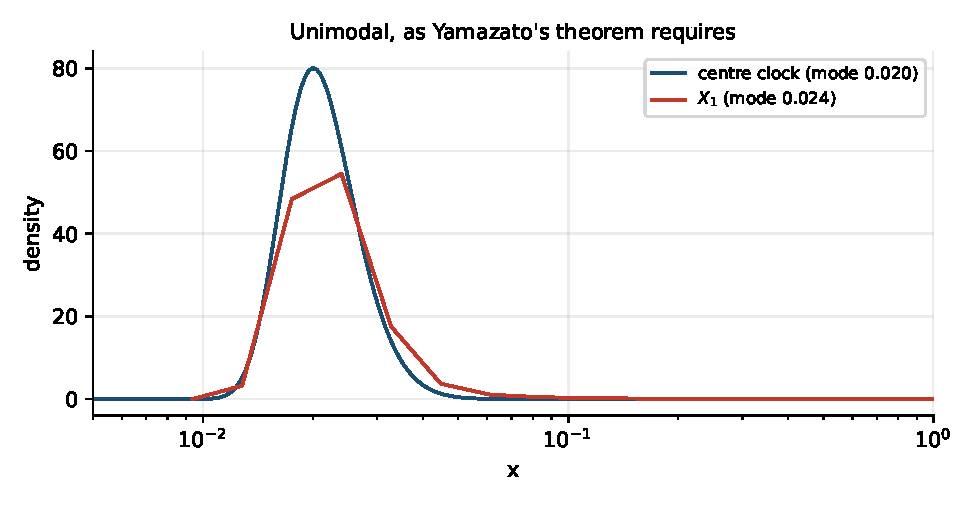
\includegraphics[width=0.75\textwidth]{fig/sb_unimodal.pdf}
\caption{The densities of the centre clock $T$ and of the shifted clock $T_1$, written $X_1$ in the plot, on a logarithmic axis. The density of $T$ is drawn on a grid of spacing $0.0005$ on $[0.004,0.4]$, from the Talbot inversion and the spectral expansion of Section~\ref{ch:clocklaw}; that of $T_1$ on the $40$ point geometric grid of the Talbot inversion behind Table~\ref{bp:tab:density}, which is why its curve is piecewise linear. The legend gives, for each, the grid point of largest density. Assembled by \texttt{comp.py} and drawn by \texttt{figs.py}, both in the folder \texttt{sato\_bondesson}.}
\label{sb:fig:unimodal}
\end{figure}

\subsection{Moments, the tail and the two ends of the Thorin measure}\label{sb:sec:tail}

Sato's moment theorem \cite[Theorem 25.3]{Sato99} says in particular that an infinitely divisible law has finite mean if and only if its L\'evy measure integrates $x$ at infinity. For a GGC with Thorin measure $U$ the L\'evy density is $x^{-1}\int e^{-xz}\,U(dz)$ (Section~\ref{sec:ch3:readings}), so the L\'evy measure $\nu_{T_1}$ of $T_1$ and its tail are, in the chart $\theta=\sqrt z$,
\begin{equation}\label{sb:eq:levy}
\nu_{T_1}(dx)=\frac{dx}x\int_0^\infty e^{-x\theta^2}\rho_{1/2}(\theta)\,d\theta,\qquad \nu_{T_1}((x,\infty))=\int_0^\infty\rho_{1/2}(\theta)\,E_1(x\theta^2)\,d\theta,
\end{equation}
where $E_1(y)=\int_y^\infty e^{-w}\,dw/w$ is the exponential integral. As $x\to\infty$ only $\theta$ near zero contributes, and $\int_0^\infty E_1(w^2)\,dw=\sqrt\pi$ gives $\nu_{T_1}((x,\infty))\sim\rho_{1/2}(0)\sqrt{\pi/x}=b_1(\pi x)^{-1/2}$, which is not integrable at infinity, so the L\'evy measure does not integrate $x$ at infinity and the mean is infinite, as Section~\ref{ch:basepoint} found. The tail is regularly varying of index $-\frac12$, so the L\'evy measure is subexponential. By the theorem of Embrechts, Goldie and Veraverbeke \cite{EGV79}, an infinitely divisible law on $[0,\infty)$ is subexponential if and only if its L\'evy measure, restricted to $(1,\infty)$ and normalised, is subexponential, and if and only if the tail of the law is asymptotic to the tail of the L\'evy measure. Hence
\begin{equation}\label{sb:eq:tail}
P(T_1>x)\sim\nu_{T_1}((x,\infty))\sim\frac{b_1}{\sqrt{\pi x}}=0.01303\,x^{-1/2},\qquad x\to\infty .
\end{equation}
This recovers the tail \eqref{bp:eq:tail}, which Section~\ref{ch:basepoint} found by a Tauberian argument, and the same reasoning, with the Thorin density $v_\alpha/\pi$ and its value $b_\alpha/\pi$ at the origin, gives $\E T_\alpha=\infty$ and the tail $b_\alpha(\pi x)^{-1/2}$ of $T_\alpha$ for every $\alpha\ge1$, and for $\frac12<\alpha<1$ whenever no zero lies to the right of $\alpha$. Theorem~\ref{bp:thm:alpha} gives the infinite mean and the tail of $T_\alpha$ for every $\alpha>\frac12$ by the Tauberian route, and since $T_\alpha$ is infinitely divisible for every $\alpha>\frac12$ (Section~\ref{sb:sec:bernstein}), the theorem of Embrechts, Goldie and Veraverbeke, read from the tail of the law to that of the L\'evy measure, shows that the L\'evy tail of $T_\alpha$ is asymptotic to $b_\alpha(\pi x)^{-1/2}$ as well, wherever the zeros lie.

Table~\ref{sb:tab:tail} and the right panel of Figure~\ref{sb:fig:tail} compare the survival function of $T_1$, computed in Section~\ref{bp:sec:rs1} by Talbot inversion near the origin and by the subordination representation beyond, with the L\'evy tail computed from \eqref{sb:eq:levy} and the Thorin density on $[0,100]$. In the bulk of the law the two differ widely: at $x=0.02$, just below the mode, the survival probability is $0.747$ while the L\'evy tail is $0.101$. Further out the survival probability exceeds the L\'evy tail by $1.2$ per cent at $x=1$, by $0.15$ per cent at $x=10$ and by $0.05$ per cent at $x=100$, and both approach the asymptote of \eqref{sb:eq:tail}; the value $\sqrt{100}\,P(T_1>100)=0.013037$ is the one found in Section~\ref{bp:sec:rs1}.

\begin{table}[htbp]
\centering\small
\begin{tabular}{rcccc}
\toprule
$x$ & $P(T_1>x)$ & $\nu_{T_1}((x,\infty))$ & ratio & $b_1(\pi x)^{-1/2}$\\
\midrule
0.1 & $4.7639\times10^{-2}$ & $4.1558\times10^{-2}$ & 1.1463 & $4.1206\times10^{-2}$\\
0.5 & $1.8907\times10^{-2}$ & $1.8458\times10^{-2}$ & 1.0243 & $1.8428\times10^{-2}$\\
1 & $1.3199\times10^{-2}$ & $1.3041\times10^{-2}$ & 1.0121 & $1.3030\times10^{-2}$\\
10 & $4.1272\times10^{-3}$ & $4.1209\times10^{-3}$ & 1.0015 & $4.1206\times10^{-3}$\\
100 & $1.3037\times10^{-3}$ & $1.3030\times10^{-3}$ & 1.0005 & $1.3030\times10^{-3}$\\
\bottomrule
\end{tabular}
\caption{The subexponential principle for $T_1$: the tail of the law is asymptotic to the tail of its L\'evy measure. The survival function is that of Section~\ref{bp:sec:rs1}, the L\'evy tail is computed from \eqref{sb:eq:levy} with the Thorin density $\rho_{1/2}$ tabulated on $[0,100]$ by \texttt{compute.py} of Section~\ref{ch:basepoint}, the ratio is that of the second column to the third, and the last column is the common asymptote of \eqref{sb:eq:tail}. Computed by \texttt{comp.py} in the folder \texttt{sato\_bondesson}.}
\label{sb:tab:tail}
\end{table}

\begin{figure}[htbp]
\centering
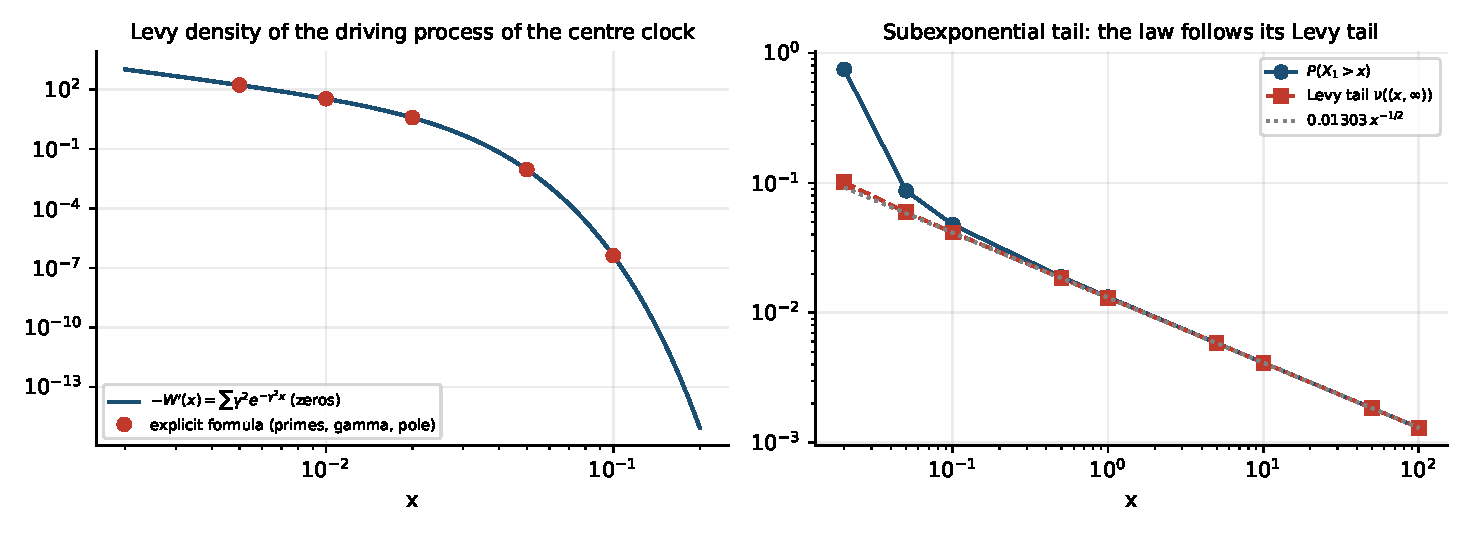
\includegraphics[width=\textwidth]{fig/sb_bdlp_tail.pdf}
\caption{Left: the L\'evy density $h=-W'$ of the driving process of the centre clock on $[0.002,0.2]$, with the heat time $t$ written $x$ in the plot, from the first $1700$ zeros (curve) and from the explicit formula at the five points of Table~\ref{sb:tab:bdlp} (dots). Right: the survival function of $T_1$, written $P(X_1>x)$ in the plot, its L\'evy tail $\nu_{T_1}((x,\infty))$, written $\nu((x,\infty))$, and their common asymptote $b_1(\pi x)^{-1/2}=0.01303\,x^{-1/2}$, at $x=0.02$, $0.05$, $0.1$, $0.5$, $1$, $5$, $10$, $50$ and $100$. Computed by \texttt{weil.py} and \texttt{comp.py} and drawn by \texttt{figs.py}, all in the folder \texttt{sato\_bondesson}.}
\label{sb:fig:tail}
\end{figure}

Bondesson's results on the two ends of the Thorin measure explain the shape of $T_1$: for a GGC the behaviour of the Thorin measure near zero governs the right tail, and its total mass governs the density at the origin \cite{Bondesson}. At the basepoint one the Thorin measure $U_1$ of $T_1$ (Proposition~\ref{bp:prop:thorin}) has $U_1((0,z])=\int_0^{\sqrt z}\rho_{1/2}(\theta)\,d\theta\sim(b_1/\pi)\sqrt z$ as $z\downarrow0$, since $\rho_{1/2}(0)=b_1/\pi$. The substitution $z=uw$ in $-\log\varphi_1(u)=\int\log(1+u/z)\,U_1(dz)$, together with $\int_0^\infty\log(1+1/w)\,d\sqrt w=\pi$, then gives $1-\varphi_1(u)\sim b_1\sqrt u$ as $u\downarrow0$, the Tauberian form of the tail \eqref{sb:eq:tail} and the expansion from which Section~\ref{ch:basepoint} derived \eqref{bp:eq:tail}. At the other end the total mass is infinite, since $U_1((0,Y^2])=M_{1/2}(Y)$ differs from the number $N(Y)$ of zeros with ordinates in $(0,Y]$ by the term $\tau_{1/2}(Y)=O(\log Y)$ of Section~\ref{bp:sec:thorin}, and this is why $T_1$, like the centre clock (Section~\ref{sec:ch19:zones}), is super flat at the origin: its density vanishes faster than any power. Indeed, for every $z_0>0$ the Thorin form gives $\varphi_1(u)\le(1+u/z_0)^{-U_1((0,z_0])}$, and $U_1((0,z_0])\to\infty$ as $z_0\to\infty$, so $\varphi_1(u)$ decays faster than any power of $u$. Markov's inequality $P(T_1\le x)\le e\,\varphi_1(1/x)$ carries this to the distribution function, and since the density $f_{T_1}$ is nondecreasing up to the mode (Corollary~\ref{sb:cor:unimodal}), the bound $xf_{T_1}(x)\le P(T_1\le2x)$ for small $x$ carries it to the density.

\subsection{Uniqueness and quasi infinite divisibility}\label{sb:sec:qid}

The L\'evy Khintchine triplet of an infinitely divisible law is unique \cite[Theorem 8.1]{Sato99}, and when the L\'evy measure has exponential moments it is also determined by the second derivative of the logarithm of the Laplace transform, through the uniqueness of the inverse Laplace transform. Lindner, Pan and Sato \cite{LPS18} call a law quasi infinitely divisible if its characteristic function is the quotient of two infinitely divisible characteristic functions, equivalently if it has a L\'evy Khintchine form with a signed measure $\nu^+-\nu^-$ whose parts $\nu^+$ and $\nu^-$ are both L\'evy measures, so in particular of finite mass away from the origin; the Gaussian coefficient is still nonnegative \cite[Lemma 2.7]{LPS18}, and the triplet is again unique. Their theory places the tilted P\'olya variables $V_\alpha$ precisely. The signed measures in question are those of the L\'evy forms of Section~\ref{bp:sec:levy}: for $\alpha\ge1$,
\[
\log\frac{\xi(\alpha+s)}{\xi(\alpha)}=b_\alpha s+\int_0^\infty\big(e^{-sx}-1+sx\big)\,\Pi_\alpha(dx),
\]
which at $\alpha=1$ is \eqref{bp:eq:levyform}, a compensated limit, and which for $\alpha>1$ converges absolutely when $\re s>1-\alpha$. For $\alpha>1$, read at $s=it$, it is a L\'evy Khintchine form for the characteristic function of $V_\alpha$, with the measure $\Pi_\alpha$ carried to the negative half line by the reflection $x\mapsto-x$. We write $x_*=0.28120$ for the root of $e^{-3x}=1-e^{-2x}$, which is the logarithm of the real root $1.32472$ of $y^3=y+1$, the plastic number.

\begin{proposition}\label{sb:prop:qid}
\begin{enumerate}
\item The P\'olya variable $X=V_{1/2}$ is not quasi infinitely divisible, since its characteristic function $\Xi(t)/\Xi(0)$ vanishes at the ordinates.
\item For every $\alpha>1$, $V_\alpha$ is quasi infinitely divisible and not infinitely divisible. Its signed L\'evy measure is the reflection to the negative half line of
\[
\Pi_\alpha(dx)=\Big(\frac{e^{-(\alpha+2)x}}{1-e^{-2x}}-e^{-(\alpha-1)x}\Big)\frac{dx}x+\sum_n\frac{\Lambda(n)}{n^\alpha\log n}\,\delta_{\log n}(dx),
\]
whose atoms have total mass $\log\zeta(\alpha)$ and whose absolutely continuous part is positive on $(0,x_*)$ and negative beyond. The negative part of $\Pi_\alpha$ is therefore carried by $(x_*,\infty)$, and its mass on $(1,\infty)$ is $E_1(\alpha-1)-\sum_{k\ge0}E_1(\alpha+2+2k)$: it is dominated by the pole term $e^{-(\alpha-1)x}dx/x$, of mass $E_1(\alpha-1)$ on $(1,\infty)$, but is not equal to it.
\item At $\alpha=1$, $V_1$ is not quasi infinitely divisible. The candidate measure $\Pi_1$ of Proposition~\ref{bp:prop:levy} has the pole term $-dx/x$ and the prime atoms $\Lambda(n)/(n\log n)$ at $\log n$, each of infinite mass on $(1,\infty)$; since the gamma density $e^{-3x}(1-e^{-2x})^{-1}/x$ is less than $0.06/x$ there, the positive and the negative part of $\Pi_1$ both have infinite mass on $(1,\infty)$, and its L\'evy form converges only as a compensated limit, which exists by the prime number theorem.
\end{enumerate}
\end{proposition}

Items (1) and (2) are due to Nakamura \cite{Nakamura15}: (2), with the same measure, is his Theorem 1.4, and (1) is the remark after it.

\begin{proof}
(1) A quasi infinitely divisible characteristic function is the exponential of the finite exponent of its L\'evy Khintchine form, so it never vanishes, while $\E e^{itX}=\Xi(t)/\Xi(0)$ by \eqref{eq:ch2:mgf}, which vanishes at $t=14.134725$ and at every other ordinate of a zero on the critical line.

(2) Let $\alpha>1$. Every piece of the L\'evy form then converges absolutely, and each piece is a L\'evy measure: the positive density $e^{-(\alpha+2)x}(1-e^{-2x})^{-1}dx/x$, the pole term and the atoms. The factorisation of $\xi$ exhibits the two infinitely divisible laws of the definition. Removing the factor $s(s-1)$ from $\xi(s)=\frac12s(s-1)\pi^{-s/2}\Gamma(\frac s2)\zeta(s)$ gives, for $\re s>1-\alpha$,
\[
\frac{\xi(\alpha+s)}{\xi(\alpha)}\cdot\frac{\alpha}{\alpha+s}\cdot\frac{\alpha-1}{\alpha-1+s}=\pi^{-s/2}\,\frac{\Gamma(\frac{\alpha+s}2)}{\Gamma(\frac\alpha2)}\,\frac{\zeta(\alpha+s)}{\zeta(\alpha)} .
\]
Let $e_1$ and $e_2$ be standard exponential variables, $\Gamma_{\alpha/2}$ a gamma variable of shape $\frac\alpha2$ and unit scale, and $\mathcal Z_\alpha$ a variable with the zeta law $P(\mathcal Z_\alpha=n)=n^{-\alpha}/\zeta(\alpha)$, all independent of each other and of $V_\alpha$. Since $\E e^{-se_1/\alpha}=\alpha/(\alpha+s)$, $\E\Gamma_{\alpha/2}^{s/2}=\Gamma(\frac{\alpha+s}2)/\Gamma(\frac\alpha2)$ and $\E\mathcal Z_\alpha^{-s}=\zeta(\alpha+s)/\zeta(\alpha)$, the identity says that
\[
V_\alpha-\frac{e_1}\alpha-\frac{e_2}{\alpha-1}\stackrel d=\frac12\log\Gamma_{\alpha/2}-\frac12\log\pi-\log\mathcal Z_\alpha .
\]
The right side is infinitely divisible: $\frac12\log\Gamma_{\alpha/2}$ has, by Binet's formula \cite[\S5.9]{DLMF} as in the proof of Proposition~\ref{bp:prop:levy}, the L\'evy measure $e^{-\alpha x}(1-e^{-2x})^{-1}dx/x$ reflected to the negative half line, and by the Euler product $-\log\mathcal Z_\alpha$ is compound Poisson with L\'evy measure $\sum_n\Lambda(n)(n^\alpha\log n)^{-1}\delta_{-\log n}$, of total mass $\log\zeta(\alpha)$. The variable $-e_1/\alpha-e_2/(\alpha-1)$ is infinitely divisible as well, with L\'evy measure $(e^{-\alpha x}+e^{-(\alpha-1)x})\,dx/x$ reflected, so the law of $V_\alpha$ convolved with an infinitely divisible law is infinitely divisible, and $V_\alpha$ is quasi infinitely divisible. Its signed L\'evy measure is the difference of the two L\'evy measures, which is $\Pi_\alpha$ reflected, since $e^{-\alpha x}(1-e^{-2x})^{-1}-e^{-\alpha x}=e^{-(\alpha+2)x}(1-e^{-2x})^{-1}$. The absolutely continuous part of $\Pi_\alpha$ has the density $e^{-(\alpha-1)x}\big(e^{-3x}(1-e^{-2x})^{-1}-1\big)x^{-1}$, whose sign is that of $e^{-3x}-(1-e^{-2x})$ whatever $\alpha$ is: positive on $(0,x_*)$ and negative beyond, where it is at least $-e^{-(\alpha-1)x}/x$, whose integral over $(1,\infty)$ is $E_1(\alpha-1)$; expanding $(1-e^{-2x})^{-1}$ in powers of $e^{-2x}$ and integrating termwise over $(1,\infty)$ gives the mass of the negative part there. If $V_\alpha$ were infinitely divisible, uniqueness of the triplet \cite[Theorem 8.1]{Sato99}, applied to the identity in law above, would make its L\'evy measure equal to $\Pi_\alpha$ reflected, which is negative on the reflection of $(x_*,\log2)$, an interval that carries no atom. So $V_\alpha$ is not infinitely divisible.

(3) Suppose that $V_1$ is quasi infinitely divisible, so that $\E e^{itV_1}=\exp\Psi_{V_1}(t)$ with
\[
\Psi_{V_1}(t)=ict-\frac A2t^2+\int_{\R}\big(e^{ity}-1-ity\mathbf 1\{|y|\le1\}\big)\,\mu(dy),
\]
where $A$ and $c$ are real and $\mu$ is a signed measure on $\R\setminus\{0\}$ with $\int\min(1,y^2)\,|\mu|(dy)<\infty$. As in (1), the characteristic function never vanishes, so $\xi(1+it)\ne0$ for real $t$; and $\xi(1+s)\ne0$ for $\re s>0$ by the Euler product. So $\ell(s)=\log(\xi(1+s)/\xi(1))$, with $\ell(0)=0$, is a continuous logarithm on the closed half plane $\re s\ge0$, holomorphic inside, and $\Psi_{V_1}(t)=\ell(it)$, since both are continuous logarithms of $\xi(1+it)/\xi(1)$ that vanish at $t=0$. For $r>0$ put $\Delta_rF(t)=F(t+r)+F(t-r)-2F(t)$. Then
\[
\Delta_r\Psi_{V_1}(t)=\int_{\R}e^{ity}\,\lambda_r(dy),\qquad \lambda_r(dy)=-Ar^2\delta_0(dy)+(2\cos ry-2)\,\mu(dy),
\]
and $\lambda_r$ is a finite signed measure because $|2\cos ry-2|\le\min(4,r^2y^2)$. On the other side, let $\check\Pi_1$ be the reflection of $\Pi_1$ to the negative half line. For $\sigma>0$ the variable $V_{1+\sigma}$ has the characteristic function $\exp(\ell(\sigma+it)-\ell(\sigma))$, and by (2) its signed L\'evy measure is the reflection of $\Pi_{1+\sigma}(dx)=e^{-\sigma x}\Pi_1(dx)$, that is $e^{\sigma y}\check\Pi_1(dy)$. The second difference removes the drift and the compensator, so
\[
\Delta_r\ell(\sigma+i\,\cdot\,)(t)=\int_{\R}e^{ity}\,m_\sigma(dy),\qquad m_\sigma(dy)=e^{\sigma y}(2\cos ry-2)\,\check\Pi_1(dy),
\]
where $m_\sigma$ is a finite signed measure, the atoms contributing at most $4\log\zeta(1+\sigma)$ to its total variation. As $\sigma\downarrow0$, $m_\sigma$ tends to $m_0=(2\cos ry-2)\,\check\Pi_1$ in the space of tempered distributions, by dominated convergence, because $|m_0|$ is locally finite and $|m_0|((-R,0))=O(R)$ as $R\to\infty$: the factor $2\cos ry-2$ tames $\check\Pi_1$ near the origin, and $\Lambda(n)\le\log n$ bounds the atom at $-\log n$ by $1/n$. So the Fourier transforms converge as tempered distributions. On the other hand $\Delta_r\ell(\sigma+it)\to\Delta_r\Psi_{V_1}(t)$ uniformly for $t$ in compact sets, because $\ell$ is uniformly continuous on compact subsets of the closed half plane. Hence the Fourier transforms of $m_0$ and $\lambda_r$ agree on smooth test functions of compact support, which are dense in the Schwartz space, so they agree as tempered distributions, and since the Fourier transform is injective there, $m_0=\lambda_r$ as measures. The mass at the origin gives $A=0$. On a compact set $K\subset\R\setminus\{0\}$, $2\cos ry-2<0$ once $r<2\pi/\max_K|y|$, so $\mu=\check\Pi_1$ on $K$, and hence on $\R\setminus\{0\}$. But the atom of $\Pi_1$ at $\log p$ has mass $1/p$, so $|\mu|((-\infty,-1))\ge\sum_{p\ge3}1/p=\infty$, and $|\mu|$ is not a L\'evy measure. This contradiction proves (3).
\end{proof}

In the identity in law used for (2) the two infinitely divisible witnesses fail together at $\alpha=1$: the exponential variable $e_2/(\alpha-1)$, which carries the pole of $\zeta$, and the zeta law of $\mathcal Z_\alpha$, which carries the primes, both cease to exist. So quasi infinite divisibility is lost exactly at the basepoint one, the same place where the prime number theorem becomes necessary and where the L\'evy form turns from absolutely to conditionally convergent.

The proof of (3) uses about the primes only the Euler product, and not the prime number theorem: the nonvanishing of $\zeta$ on the line $\re s=1$, the first step towards that theorem, enters only through the hypothesis, which forces it. The existence of the compensated limit in (3) needs more. Of the two estimates that the proof of Proposition~\ref{bp:prop:levy} uses for it, the second is the logarithm of Mertens' product theorem \cite[Theorem 429]{boHardyWright} and gives the cancellation of zeroth order between the prime atoms and $dx/x$, while the first, which the compensator $sx$ requires, is a form of the prime number theorem, whose analytic proof rests on $\zeta(1+it)\ne0$ \cite{Titchmarsh}. Below the basepoint one the L\'evy form exists only if there is a zero free half plane (Proposition~\ref{bp:prop:below}).

Section~\ref{bp:sec:levy} reads the conclusion of (3) from the L\'evy form itself, and the proof of (3) supplies the uniqueness on which that reading rests, namely that no other signed measure can represent the same characteristic function. Since an infinitely divisible law is quasi infinitely divisible, (3) also shows directly that $V_1$ is not infinitely divisible, which is how that section concludes. The same argument, with $\xi(1+s,\chi_{12})$ in place of $\xi(1+s)$, shows that the tilted eta variable of Section~\ref{bp:eta:sec:levy} is neither quasi infinitely divisible nor infinitely divisible, as that section argues: its L\'evy form has the atoms $\chi_{12}(n)\Lambda(n)/(n\log n)$ at $\log n$, of absolute value $1/p$ at $\log p$ for every prime $p\ge5$, and by Dirichlet's theorem those with $\chi_{12}(n)=1$ and those with $\chi_{12}(n)=-1$ both have infinite mass.

\subsection{Bondesson's classes and Thorin Bernstein functions}\label{sb:sec:bernstein}

By Bondesson's characterisation, recalled in Section~\ref{sec:ch3:hierarchy}, a function with limit one at the origin is the Laplace transform of a GGC if and only if it is hyperbolically completely monotone \cite[Theorem 6.1.1]{Bondesson}, and the class of HCM densities is closed under products and quotients of independent variables and under powers $X^q$ with $|q|\ge1$ \cite[Section 5.1]{Bondesson}. These are the tools behind the Bosch threshold of Theorem~\ref{bs:thm:power}: $\varphi_{1/2}(u^{1/\beta})$ is HCM exactly when $|\beta|\ge1/(1-\alpha_\xi)$, where $\alpha_\xi=2\delta_*/\pi$ and $\delta_*$ is the largest angle $|\arg\gamma|$ over the zeros $\gamma$ of $\Xi$ with $\re\gamma>0$. RH is the statement $\alpha_\xi=0$.

The class of GGCs is closed under weak limits (Section~\ref{sec:weak:limits}), which gives the closure criterion of Corollary~\ref{cor:weak:closure} used for the Kent approximants of Section~\ref{sec:ch18:kent}. Bondesson also treats mixtures of exponential laws and their generalised convolutions. This is the natural class for Kent's hitting times started from an interior point: for a diffusion started at $x_0$ and a level $y_0>x_0$ the Laplace transform of the first passage time to $y_0$ is $\psi_u(x_0)/\psi_u(y_0)$, where $\psi_u$ is the increasing positive solution of $\mathcal A\psi=u\psi$ for the generator $\mathcal A$ of the diffusion, and it is a ratio of two products with interlacing zeros. The law of $T_1$ is not a mixture of exponentials, since a mixture of exponentials has a completely monotone density while that of $T_1$ vanishes at the origin and has an interior mode (Figure~\ref{sb:fig:unimodal}). This is consistent with the conclusion of Section~\ref{ch:bphit} that $T_1$ is a subordinated rather than a direct Kent hitting time (Section~\ref{bp:sec:kent} and Theorem~\ref{bp:thm:sub}).

In the language of Schilling, Song and Vondra\v{c}ek \cite[Definition 9.10]{boSSV}, a law on $[0,\infty)$ is a GGC exactly when its Laplace exponent is a Thorin Bernstein function, equivalently when the derivative of the exponent is a Stieltjes function, the function $f_H$ of Section~\ref{sec:ch3:readings}. The Laplace exponent of the centre clock is $\log G$, a Bernstein function with no hypothesis because $T$ is infinitely divisible; we give it no separate name, since $G$ already denotes the reciprocal of its Laplace transform. The subordination identity of Theorem~\ref{bp:thm:alpha} reads
\begin{equation}\label{sb:eq:comp}
\begin{gathered}
-\log\varphi_\alpha(u)=\log G\big((\alpha-\tfrac12)^2+f_\alpha(u)\big)-\log G\big((\alpha-\tfrac12)^2\big),\\
f_\alpha(u)=u+2(\alpha-\tfrac12)\sqrt u,
\end{gathered}
\end{equation}
with $f_\alpha$, the Laplace exponent of the subordinator $\sigma^{(\alpha)}$ of that theorem, a complete Bernstein function. The derivative $\frac{d}{du}[-\log\varphi_\alpha(u)]=\frac1{2\sqrt u}\frac{\xi'}{\xi}(\alpha+\sqrt u)$ is a Stieltjes function exactly when no zero lies to the right of $\alpha$, that is when $\alpha\ge\sup_\rho\re\rho$, which is the criterion of Theorem~\ref{thm:poisson}: a zero with $\re\rho>\alpha$ makes $\xi(\alpha+\sqrt u)$ vanish at the point $u=(\rho-\alpha)^2$ of the cut plane $\cut$, where a Stieltjes function is holomorphic. This is a statement about the analytic continuation of the exponent, and not about the sign of the Thorin density $v_\alpha/\pi$ on the single line $\re s=\alpha$, which is not known to exclude zeros to the right of that line (Remark~\ref{rem:ch2:oneline}).

\begin{proposition}\label{sb:prop:tbf}
For every $\alpha\ge1$ the composition $\log G((\alpha-\frac12)^2+f_\alpha)-\log G((\alpha-\frac12)^2)$ is a Thorin Bernstein function with no hypothesis, while $\log G$ itself is a Thorin Bernstein function if and only if RH holds. For $\frac12<\alpha<1$ the composition is a Thorin Bernstein function if and only if $\zeta$ has no zeros with real part greater than $\alpha$.
\end{proposition}

\begin{proof}
By \eqref{sb:eq:comp} the composition is the Laplace exponent of $T_\alpha$, so it is a Thorin Bernstein function exactly when $T_\alpha$ is a GGC, which by Theorem~\ref{thm:poisson} happens exactly when no zero has real part greater than $\alpha$. For $\alpha\ge1$ there is none, since $\zeta$ has no zeros on or to the right of the line $\re s=1$. The exponent $\log G$ is a Thorin Bernstein function exactly when $T$ is a GGC, which is RH by Proposition~\ref{prop:rigid}.
\end{proof}

For every $\alpha>\frac12$ the composition is at least a Bernstein function: $u\mapsto\log G((\alpha-\frac12)^2+u)-\log G((\alpha-\frac12)^2)$ is the Laplace exponent of the tilted clock $\widetilde T_\alpha$, and a Bernstein function composed with a Bernstein function is again one \cite[Corollary 3.8]{boSSV}. So $T_\alpha$ is infinitely divisible for every $\alpha>\frac12$ with no hypothesis, and the location of the zeros decides only whether it is a GGC. The proposition says that composing with the complete Bernstein function $f_\alpha$ creates the Thorin property from a function only known to be Bernstein. Analytically this is the Poisson smoothing of the Thorin measure by Cauchy kernels of widths $\alpha-\beta$ (Proposition~\ref{prop:struct}); probabilistically it is the stable one half subordination of Theorem~\ref{bp:thm:alpha}, by a drift plus a stable subordinator of index one half. RH is the statement that the smoothing was never needed, that is, that $\log G$ is already a Thorin Bernstein function, and the family $\alpha\downarrow\frac12$ measures how much smoothing is required at each basepoint.

General composition theorems do not settle this. For a Bernstein function $\kappa$ and $a\ge0$ let $\kappa_a(u)=\kappa((\sqrt u+a)^2)-\kappa(a^2)$, so that the composition in \eqref{sb:eq:comp} is $\kappa_a$ for $\kappa=\log G$ and $a=\alpha-\frac12$. If $\kappa$ is a Thorin Bernstein function then so is every $\kappa_a$, because the shift turns a drift $cu$ into $c(u+2a\sqrt u)$ and each factor $(1+u/t)^{-1}$ of the Thorin form into $(a^2+t)/((\sqrt u+a)^2+t)$, the Laplace transform of a GGC whose Thorin density in $\theta$ is the pair of Cauchy kernels of width $a$ at $\pm\sqrt t$, as in Section~\ref{bp:sec:sub}. Applied to $\kappa_a$, with $\kappa_{a+a'}=(\kappa_a)_{a'}$, this shows that the shifts $a$ for which $\kappa_a$ is a Thorin Bernstein function form a half line, and for $\kappa=\log G$ Proposition~\ref{sb:prop:tbf} identifies it as $[a_*,\infty)$ with $a_*=\sup_\rho\re\rho-\frac12$; RH is the statement $a_*=0$. For a fixed shift the implication cannot be reversed. The function $\kappa(u)=2\log(1+u)+\log(1+(120u+16u^2)/289)$ is a Bernstein function, since $\kappa'$ is the Laplace transform of $2e^{-x}+2e^{-15x/4}\cos2x\ge0$, and it is not a Thorin Bernstein function, since $\kappa'$ has poles at $-\frac{15}4\pm2i$, where a Stieltjes function is holomorphic; yet
\[
\kappa_{1/2}(u)=\log\Big(1+\frac u4\Big)+2\log\frac{4((\sqrt u+\frac12)^2+1)}5+\log\frac{(\sqrt u+1)^2+4}5
\]
is a Thorin Bernstein function, the exponent of an exponential law plus the exponents of GGCs whose Thorin densities are pairs of Cauchy kernels, of width $\frac12$ at $\pm1$ and of width $1$ at $\pm2$; the function $u\mapsto\kappa(u/4a^2)$ gives the same example at any shift $a>0$.

The Dirichlet mean representation of James, Roynette and Yor \cite{JRY} writes a GGC whose Thorin measure has finite total mass $c$ as the product $\Gamma_c\mathcal M$ of a gamma variable $\Gamma_c$ of shape $c$ and an independent Dirichlet mean $\mathcal M$. It applies to the truncated lattice variables $\mathcal S_n$ of Section~\ref{rz:sec:finite}, whose Thorin measures have total mass $2n$, and to the finite sums of exponential variables of Proposition~\ref{rz:prop:multlee}, but not to $T_\alpha$ or, under RH, to $T$, whose Thorin measures have infinite mass.

\subsection{What these results cannot give}\label{sb:sec:cannot}

Every GGC criterion in these books is, for the reciprocal Xi function at the centre, equivalent to RH: the HCM property of the Laplace transform and the Stieltjes property of the derivative of the exponent (Theorem~\ref{bh:thm:main}), the Pick function property (Corollary~\ref{bs:cor:rh}), and the complete monotonicity of the L\'evy density of the driving process (Proposition~\ref{sb:prop:bdlp}). The books classify laws and derive consequences once positivity of the Thorin measure is known, and the consequences obtained in Sections~\ref{sb:sec:sd} to \ref{sb:sec:bernstein}, the driving process, unimodality, the subexponential tail, quasi infinite divisibility and the Thorin Bernstein compositions, are mostly unconditional. Table~\ref{sb:tab:results} collects them with their sources.

They are unconditional for one of two reasons. Some use only the infinite divisibility and self decomposability of the centre clock, that is the inequalities $W>0$ and $W'<0$, which hold wherever the zeros above height $1000$ lie, their proof using only the verification of RH below that height (Theorem~\ref{thm:ch12:idsd}). The others use the region $\re s\ge1$, through positivity of the Thorin measure at a basepoint $\alpha\ge1$, which rests on the nonvanishing of $\zeta$ on the line $\re s=1$ (Theorem~\ref{thm:poisson}), or through the Euler product, as in Proposition~\ref{sb:prop:qid}. Neither source reaches below the basepoint one: the first cannot detect the higher zeros at all, and the second stops at the line $\re s=1$, where the Euler product ceases to converge. So none of the results supplies positivity of the Thorin measure uniformly in the height at a basepoint $\alpha<1$, in the sense of Theorem~\ref{thm:poisson} that $T_\alpha$ is a GGC, which is the zero free half plane $\re s>\alpha$ of step~7 of the path in Table~\ref{tab:ch25:path}, and still less at the centre, where it is RH itself. That positivity, uniform in the height, is the one ingredient still missing on the path to RH; the half plane $\re s>\frac78$ announced in October 2026 would supply it for every $\alpha>\frac78$, by arithmetic from outside the theory (Section~\ref{sec:ch25:open}).

\begin{table}[htbp]
\centering\small
\begin{tabular}{p{0.24\textwidth}p{0.2\textwidth}p{0.35\textwidth}p{0.09\textwidth}}
\toprule
result & source & consequence here & status\tabularnewline
\midrule
\raggedright background driving L\'evy process & \raggedright Wolfe; Jurek and Vervaat; Sato, Theorem 17.5 & \raggedright centre clock driven by a subordinator with L\'evy density $-W'$; RH if and only if it is completely monotone & proved\tabularnewline
\raggedright Yamazato's theorem & \raggedright Yamazato; Sato, Theorem 53.1 & \raggedright centre clock and $T_\alpha$, $\alpha>\frac12$, unimodal & proved\tabularnewline
\raggedright Urbanik's classes $L_n$ & \raggedright Urbanik; Sato 1980; Berg and Forst & \raggedright centre clock in $L_2$, not in $L_3$; its driving process and the driving process of that self decomposable, with unimodal marginals & proved\tabularnewline
\raggedright moment theorem & \raggedright Sato, Theorem 25.3 & \raggedright $\E T_\alpha=\infty$ for $\alpha\ge1$ & proved\tabularnewline
\raggedright subexponential tails & \raggedright Embrechts, Goldie, Veraverbeke & \raggedright $P(T_\alpha>x)\sim b_\alpha(\pi x)^{-1/2}$; ratio $1.0005$ at $x=100$ & \raggedright proved, checked\tabularnewline
\raggedright uniqueness, quasi infinite divisibility & \raggedright Sato, Theorem 8.1; Lindner, Pan, Sato & \raggedright $V_\alpha$ quasi infinitely divisible for $\alpha>1$, not at $\alpha=1$; P\'olya variable not quasi infinitely divisible & proved\tabularnewline
\raggedright HCM characterisation and closure & \raggedright Bondesson & \raggedright Bosch threshold for powers & proved\tabularnewline
\raggedright Thorin measure at the two ends & \raggedright Bondesson & \raggedright $x^{-1/2}$ tail and super flat origin & proved\tabularnewline
\raggedright Thorin Bernstein composition & \raggedright Schilling, Song, Vondra\v{c}ek & \raggedright smoothing by $f_\alpha$ creates the Thorin property for $\alpha\ge1$ & proved\tabularnewline
\raggedright Dirichlet means & \raggedright James, Roynette, Yor & \raggedright applies to truncations only & remark\tabularnewline
\bottomrule
\end{tabular}
\caption{What the books of Sato and Bondesson, and the papers around them, give the reciprocal Xi function: each result used in this section, its source, its consequence for the centre clock $T$, the shifted clocks $T_\alpha$ and the tilted P\'olya variables $V_\alpha$, and its status. Theorem numbers, here and in the text, refer to the first edition of Sato's book \cite{Sato99}.}
\label{sb:tab:results}
\end{table}

What the two books do provide is a vocabulary in which RH can be stated in several equivalent forms, each with its own tools: a subordinator whose L\'evy density must be shown to be a mixture of exponentials, a Bernstein function whose derivative must be shown to be a Stieltjes function, and a smoothing by $f_\alpha$ that must be shown to be unnecessary. Section~\ref{ch:path} collects the steps of the Thorin approach, marks each as proved, computed, announced or open, and sets out the path along which positivity would have to be carried from the basepoint one to the centre. The same laws are the marginals of stochastic processes, and Sections~\ref{pm:sec:wg} and \ref{pm:sec:map} collect these processes, with those of Sections~\ref{ch:bphit} and \ref{ch:strip}, on one map.

\subsection{Wiener gamma integrals and the Riemann Ornstein Uhlenbeck process}\label{pm:sec:wg}

A GGC is a superposition of gamma laws, and a gamma process realises the superposition pathwise. Let $(\Gamma_t)_{t\ge0}$ be a standard gamma process, the subordinator with $\E e^{-u\Gamma_t}=(1+u)^{-t}$, so that $\Gamma_t$ has the gamma law of shape $t$ and unit scale, like the variables $\Gamma_{\alpha/2}$ and $\Gamma_c$ of Sections~\ref{sb:sec:qid} and \ref{sb:sec:bernstein}. For a measurable $f\ge0$ the Wiener integral $\int_0^\infty f(t)\,d\Gamma_t$ has Laplace exponent $\int_0^\infty\log(1+uf(t))\,dt$. Let $U$ be the Thorin measure of a GGC without drift, $M(\theta)=U((0,\theta^2])$ its cumulative mass in the chart $\theta=\sqrt z$, and $M^{-1}(t)=\inf\{\theta:M(\theta)>t\}$ the right continuous inverse. The image of Lebesgue measure on $(0,M(\infty))$ under $M^{-1}$ is $dM$, so the substitution $t=M(\theta)$ turns $\int_0^\infty\log(1+u/M^{-1}(t)^2)\,dt$ into $\int\log(1+u/z)\,U(dz)$, and the GGC is the Wiener gamma integral
\begin{equation}\label{pm:eq:wg}
\int_0^\infty\frac{d\Gamma_t}{M^{-1}(t)^2},
\end{equation}
which is the Wiener gamma representation of the class \cite{JRY}. At the centre, under RH, $M$ is the zero counting function $N$, $M^{-1}(t)=\gamma_k$ for $k-1\le t<k$, the ordinates being counted in increasing order and with multiplicity, and \eqref{pm:eq:wg} is $\sum_k(\Gamma_k-\Gamma_{k-1})/\gamma_k^2$, the series $\sum_{\gamma>0}e_\gamma/\gamma^2$ of Proposition~\ref{prop:rigid}. At a basepoint $\alpha$ the count is replaced by the Poisson smoothed count $M_{\alpha-1/2}(\theta)=\pi^{-1}\int_0^\theta v_\alpha$ of Section~\ref{ch:turing}, which is $\pi^{-1}$ times the argument of $\xi$ along the line $\re s=\alpha$. For $\alpha\ge1$, $v_\alpha>0$ and $T_\alpha$ is a GGC, so with no hypothesis $T_\alpha$ is \eqref{pm:eq:wg} with $M=M_{\alpha-1/2}$; in particular $T_1$ is a gamma process integrated against the inverse of the Poisson smoothed zero count. For $\frac12<\alpha<1$ the representation holds exactly when $T_\alpha$ is a GGC, that is when no zero has real part greater than $\alpha$ (Theorem~\ref{bp:thm:alpha}), and then $M$ is $M_{\alpha-1/2}$ plus a unit jump at the ordinate of each zero on the line $\re s=\alpha$ (Theorem~\ref{rz:thm:threshold}). It needs $M_{\alpha-1/2}$ to be nondecreasing, that is $v_\alpha\ge0$ on the line $\re s=\alpha$, but for $\xi$ it is not known whether positivity on one line excludes zeros to its right (Remark~\ref{rem:ch2:oneline}).

Table~\ref{pm:tab:wg}, computed by \texttt{comp2.py}, checks the representation of $T_1$ with $2\times10^5$ draws. The Thorin mass up to height $100$, where the tabulated density $\rho_{1/2}$ of Section~\ref{ch:basepoint} ends, is cut into cells: $299$ cells of a geometric grid on $[10^{-12},0.005]$, where $M_{1/2}^{-1}$ is small and the stable one half part of $T_1$ lives, the cell $[0.005,0.01]$, and cells of length $0.005$ beyond. Each cell contributes an independent gamma variable with shape equal to its length, multiplied by the average of $M_{1/2}^{-1}(t)^{-2}$ over the cell, computed by quadrature, and the mass above height $100$ contributes its mean, computed with the Weyl density $\frac1{2\pi}\log\frac\theta{2\pi}$. At each of the four points the empirical Laplace transform is within one standard error of $\varphi_1$.

\begin{table}[htbp]
\centering\small
\begin{tabular}{cccc}
\toprule
$u$ & \begin{tabular}[b]{@{}c@{}}$\E\exp\big(-u\int_0^\infty M_{1/2}^{-1}(t)^{-2}\,d\Gamma_t\big)$,\\ Monte Carlo\end{tabular} & standard error & $\varphi_1(u)=\xi(1)/\xi(1+\sqrt u)$\\
\midrule
0.5 & 0.97240 & 0.00021 & 0.97253\\
1 & 0.95469 & 0.00025 & 0.95493\\
10 & 0.73988 & 0.00036 & 0.74016\\
100 & 0.09410 & 0.00014 & 0.09416\\
\bottomrule
\end{tabular}
\caption{The Wiener gamma representation \eqref{pm:eq:wg} of $T_1$ against the inverse of the smoothed zero count $M_{1/2}$: the empirical Laplace transform of $2\times10^5$ draws, discretised as described in the text, against $\varphi_1$. Computed by \texttt{comp2.py} in the folder \texttt{basepoint\_one/process\_map}.}
\label{pm:tab:wg}
\end{table}

Self decomposability gives a second process. If $Z$ is a subordinator with $\E\log(1+Z_1)<\infty$, the Ornstein Uhlenbeck type process $dF_t=-F_t\,dt+dZ_t$, that is $F_t=e^{-t}F_0+\int_0^te^{-(t-r)}\,dZ_r$, has a unique stationary law, the law of $\int_0^\infty e^{-t}\,dZ_t$, and every self decomposable law arises in this way from its background driving L\'evy process \cite[Theorem 17.5 and Corollary 17.9]{Sato99}. By Proposition~\ref{sb:prop:bdlp} the driving process of the centre clock is the subordinator with L\'evy density $h=-W'$, which the explicit formula computes from the primes. So there is, with no hypothesis, an Ornstein Uhlenbeck process $F$ whose stationary law is the centre clock, which we call the Riemann Ornstein Uhlenbeck process, and RH is the statement that the jump density of its driver is completely monotone. Under RH the Laplace exponent of $Z$ is $\Psi_Z(u)=u(\log G)'(u)=\sum_{\gamma>0}u/(\gamma^2+u)$, so the driver is a superposition of independent compound Poisson processes, one for each zero counted with multiplicity, each with rate one and exponential jumps of mean $\gamma^{-2}$. By the computation in the proof of Proposition~\ref{sb:prop:bdlp}, the process driven by the component of $\gamma$ has the stationary Laplace exponent $\int_0^u dw/(\gamma^2+w)=\log(1+u/\gamma^2)$, that of the exponential law of rate $\gamma^2$, and the stationary law of the sum is $\sum_{\gamma>0}e_\gamma/\gamma^2$.

The simulation by \texttt{ou.py} is exact for the $1700$ computed zeros. Jumps arrive at the times of a Poisson process of rate $1700$ on $[0,4000]$, $6.8\times10^6$ of them, each attached to a zero chosen uniformly and exponential with mean $\gamma^{-2}$; the zeros above the $1700$th enter as a drift of the driver, which adds to the stationary law the mean $\E T-\sum_{k\le1700}\gamma_k^{-2}$ of their components; between jumps the process decays exponentially, and it is sampled at spacing $0.02$ after a burn in of $20$. The time average is $0.023094$ against $\E T=\sum_ka_k^{-1}=0.023105$ (Section~\ref{bp:sec:thorin}). The empirical Laplace transform of the stationary law is $0.79520\pm0.00096$, $0.32828\pm0.00180$ and $0.016404\pm0.00030$ at $u=10$, $50$ and $200$, with standard errors from $100$ batch means, against $\varphi_{1/2}(u)=\xi(\frac12)/\xi(\frac12+\sqrt u)=0.79514$, $0.32827$ and $0.016399$. The stationary process at time $\tau\ge0$ is $e^{-\tau}$ times its value at time $0$ plus a variable independent of that value, and the centre clock has finite variance, so the autocorrelation at lag $\tau$ is $e^{-\tau}$ with no hypothesis. The estimates at lags $0.5$, $1$ and $2$ are $0.602$, $0.352$ and $0.119$ against $0.607$, $0.368$ and $0.135$; the deficits are within $1.6$ standard errors of the estimates, which are about $0.008$, $0.010$ and $0.013$ by batch estimates over $20$ blocks of the same run. The top right panel of Figure~\ref{pm:fig:paths} shows ten units of time of the path.

For $\alpha\ge1$ the shifted clock $T_\alpha$ is a GGC, hence self decomposable, and has its own driver: by \eqref{sb:eq:levy}, with $v_\alpha/\pi$ in place of $\rho_{1/2}$, its L\'evy measure is $k_\alpha(x)\,dx/x$ with $k_\alpha(x)=\pi^{-1}\int_0^\infty e^{-x\theta^2}v_\alpha(\theta)\,d\theta$, and its driver has the completely monotone L\'evy density $-k_\alpha'(x)=\pi^{-1}\int_0^\infty\theta^2e^{-x\theta^2}v_\alpha(\theta)\,d\theta$. For $\frac12<\alpha<1$ the process exists as well, because $T_\alpha$ is self decomposable with no hypothesis (Corollary~\ref{bp:cor:levyalpha}); its driver has the L\'evy density $-W_\alpha'$, which is completely monotone exactly when $T_\alpha$ is a GGC.

\begin{figure}[htbp]
\centering
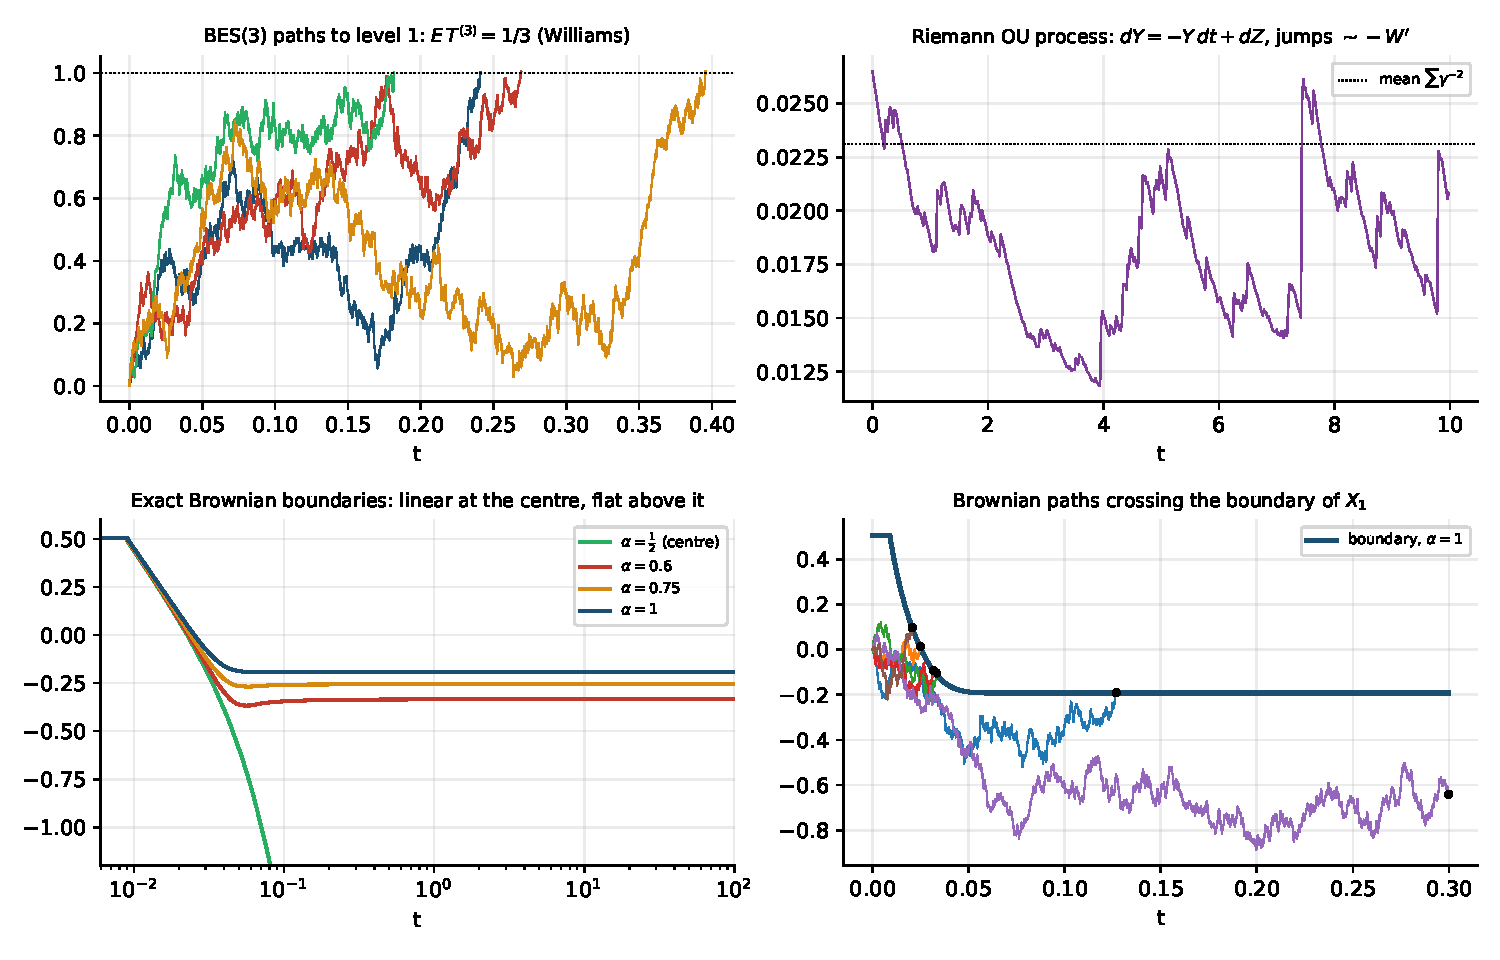
\includegraphics[width=\textwidth]{fig/bp1_paths.pdf}
\caption{Four processes of the map. Top left: paths of a three dimensional Bessel process run until they reach the level one; the hitting time has mean $\frac13$, and two independent copies make up the variable $S_2$ of Section~\ref{bp:sec:mellin}. Top right: ten units of time of the Riemann Ornstein Uhlenbeck process $F$, written $Y$ in the plot, whose stationary law is the centre clock, with the mean $\E T$, written $\sum\gamma^{-2}$ in the plot. Bottom left: the exact Brownian boundaries of $T_\alpha$ at $\alpha=\frac12$, $0.6$, $0.75$ and $1$, those at $0.6$ and $0.75$ computed under RH beyond $t=0.03$ (Section~\ref{bp:sec:across}), asymptotically linear at the centre and flat above it. Bottom right: Brownian paths crossing the boundary of $T_1$, written $X_1$ in the plot (Section~\ref{bp:sec:rs1}). Drawn by \texttt{figs.py} in the folder \texttt{basepoint\_one/process\_map} from the output of \texttt{ou.py}, the boundaries of \texttt{bnd\_alpha.py} at $\alpha=0.6$ and $0.75$, and those of Sections~\ref{ch:boundaries} and \ref{ch:bphit} at the centre and at the basepoint one.}
\label{pm:fig:paths}
\end{figure}

\subsection{Subordinated Brownian motion and the map of processes}\label{pm:sec:map}

Running an independent standard Brownian motion $B$ on a clock gives a symmetric law with
\[
\E e^{iuB_{T_\alpha}}=\E e^{-u^2T_\alpha/2}=\frac{\xi(\alpha)}{\xi(\alpha+|u|/\sqrt2)},\qquad u\in\R,
\]
so $B_{T_\alpha}$ has the law of $Y_\alpha/\sqrt2$, the normal scale mixture of Proposition~\ref{sm:prop:cf}, and what Section~\ref{ch:strip} proves for $Y_\alpha$ carries over with a factor $\sqrt2$. The characteristic function exists at every basepoint with no hypothesis. At the centre $B_T$ has the finite variance $\E T$; above it the characteristic function has a corner at the origin, $B_{T_\alpha}$ lies in the domain of attraction of the Cauchy law, and $P(|B_{T_\alpha}|>y)\sim\sqrt2\,b_\alpha/(\pi y)$ as $y\to\infty$. The law is a symmetric EGGC exactly when $T_\alpha$ is a GGC (Theorems~\ref{sm:thm:thorin} and \ref{sm:thm:strip}), and under RH at the centre it is the sum $\sum_kL_k/(\sqrt2\gamma_k)$ of scaled Laplace variables. Its Cauchy factor, of scale $b_\alpha/\sqrt2$, comes from the constant $b_\alpha/\pi=v_\alpha(0)/\pi$ of the Thorin density wherever the Thorin form \eqref{sm:eq:thorin} holds, and the planar Brownian reading of Section~\ref{bp:sec:planar} holds at every basepoint $\alpha$ to the right of every zero: $v_\alpha(\theta)\,d\theta/\pi=\sum_\rho P(B^2_H\in d\theta\mid B_0=\rho)$, where $B=(B^1,B^2)$ is a planar Brownian motion and $H$ is now its first time to reach the line $\re s=\alpha$. So the constant $b_\alpha/\pi$ is the density at $\theta=0$ of this sum of harmonic measures. Table~\ref{pm:tab:bm}, computed by \texttt{comp2.py}, checks the characteristic function and the tail at three basepoints with $3\times10^5$ draws of $T_\alpha$ each, from the subordination identity, with the tilted clock drawn as for Table~\ref{sm:tab:mc}.

\begin{table}[htbp]
\centering\small
\setlength{\tabcolsep}{4pt}
\begin{tabular}{ccccccc}
\toprule
$\alpha$ & \begin{tabular}[b]{@{}c@{}}$u=1$,\\ Monte Carlo\end{tabular} & exact & \begin{tabular}[b]{@{}c@{}}$u=3$,\\ Monte Carlo\end{tabular} & exact & $y\,P(|B_{T_\alpha}|>y)$, $y=10$ & $\sqrt2\,b_\alpha/\pi$\\
\midrule
0.6 & 0.98546 & 0.98530 & 0.89322 & 0.89286 & 0.0024 & 0.0021\\
0.75 & 0.98050 & 0.98049 & 0.87989 & 0.87994 & 0.0050 & 0.0052\\
1 & 0.97273 & 0.97253 & 0.85933 & 0.85888 & 0.0095 & 0.0104\\
\bottomrule
\end{tabular}
\caption{The characteristic function $\xi(\alpha)/\xi(\alpha+|u|/\sqrt2)$ of subordinated Brownian motion, estimated by the mean of $\cos(uB_{T_\alpha})$ over $3\times10^5$ draws at each basepoint, and its Cauchy type tail; the tail estimates rest on $72$, $149$ and $284$ exceedances of $y=10$. Computed by \texttt{comp2.py} in the folder \texttt{basepoint\_one/process\_map}.}
\label{pm:tab:bm}
\end{table}

Figure~\ref{pm:fig:map} and Table~\ref{pm:tab:map} arrange the processes of Chapter~\ref{chap:basepoint} and of this section by basepoint; we write $a=\alpha-\frac12$. The Mellin side is the Bessel picture of Williams \cite{Williams90} and of Biane, Pitman and Yor \cite{BPY01}: $S_2$, the sum of two independent hitting times of the level one by a three dimensional Bessel process, satisfies $\E(\pi S_2/2)^{s/2}=2\xi(s)$ (Section~\ref{ch:clock}), and $V_\alpha$ is $\frac12\log(\pi S_2/2)$ under the law of $S_2$ size biased by $S_2^{\alpha/2}$ (Section~\ref{bp:sec:mellin}). The clock side starts from the centre clock, which under RH with simple zeros is Kent's hitting time for a string with spectrum $\{\gamma^2\}$, and passes through the tilt $e^{-a^2T}$ and the sticky Brownian subordination of Theorem~\ref{bp:thm:alpha} to $T_\alpha$. From $T_\alpha$ it continues to the Wiener gamma integral of Section~\ref{pm:sec:wg}, to Brownian motion run on the clock, and to the Brownian boundaries of Section~\ref{bp:sec:across}, which are asymptotically linear at the centre and, at the basepoints computed, flat above it, with the Wald defect $\E\,b(T_\alpha)=b_\alpha/\sqrt2$ in place of Wald's identity when the boundary is bounded at infinity.

\begin{figure}[htbp]
\centering
\begin{tikzpicture}[node distance=0.55cm and 0.35cm, every node/.style={font=\footnotesize}, box/.style={draw, rounded corners, align=center, minimum width=3.9cm, minimum height=0.8cm, inner sep=2pt}, arr/.style={-latex, thick}]
\node[box, fill=blue!8] (bes) {two $\mathrm{BES}(3)$ hitting times\\ $S_2$, mean $\frac23$\\ (Williams; Biane, Pitman, Yor)};
\node[box, fill=blue!8, right=1.6cm of bes] (polya) {P\'olya variable $V_{1/2}$ and\\ size biased $V_\alpha$ ($S_2^{\alpha/2}$)};
\node[box, fill=green!10, below=of bes] (clock) {centre clock $T$, infinitely\\ divisible and self decomposable\\ with no hypothesis};
\node[box, fill=green!10, right=1.6cm of clock] (kent) {Kent string, spectrum $\gamma^2$\\ (under RH, simple zeros)};
\node[box, fill=orange!12, below=of clock] (sub) {tilt $e^{-a^2T}$, then sticky Brownian\\ inverse local time $u+2a\sqrt u$};
\node[box, fill=orange!12, right=1.6cm of sub] (xa) {$T_\alpha$: GGC if and only if\\ no zero has $\beta>\alpha$};
\node[box, fill=red!8, below=of sub] (ou) {Ornstein Uhlenbeck process\\ driven by $Z$, jump density $-W'$};
\node[box, fill=red!8, right=1.6cm of ou] (wg) {Wiener gamma integral\\ against the smoothed count};
\node[box, fill=gray!10, below=of ou] (bm) {$B_{T_\alpha}$: characteristic function\\ $\xi(\alpha)/\xi(\alpha+|u|/\sqrt2)$};
\node[box, fill=gray!10, right=1.6cm of bm] (bd) {Brownian boundary: asymptotically\\ linear ($\alpha=\frac12$), flat where\\ computed ($\alpha>\frac12$)};
\draw[arr] (bes) -- node[above,font=\scriptsize]{Mellin} (polya);
\draw[arr] (bes) -- node[left]{$1/\Xi$} (clock);
\draw[arr] (clock) -- (kent);
\draw[arr] (clock) -- (sub);
\draw[arr] (sub) -- (xa);
\draw[arr] (clock.west) to[bend right=35] (ou.west);
\draw[arr] (xa) -- (wg);
\draw[arr] (xa) -- (bm);
\draw[arr] (xa.east) to[bend left=35] (bd.east);
\end{tikzpicture}
\caption{Processes attached to $\xi(\alpha+\cdot)$, with $a=\alpha-\frac12$. By rows from the top: the Mellin side, the centre clock, the basepoint clocks, and two rows of further representations. Drawn in TikZ from Table~\ref{pm:tab:map}.}
\label{pm:fig:map}
\end{figure}

\begin{table}[htbp]
\centering\scriptsize
\setlength{\tabcolsep}{3pt}
\begin{tabular}{p{0.15\textwidth}p{0.18\textwidth}p{0.2\textwidth}p{0.18\textwidth}p{0.17\textwidth}}
\toprule
 & \raggedright $\alpha=\frac12$ & \raggedright $\frac12<\alpha<1$ & \raggedright $\alpha=1$ & $\alpha>1$\tabularnewline
\midrule
\raggedright Mellin side & \raggedright P\'olya variable, $S_2^{1/4}$ bias & \raggedright $S_2^{\alpha/2}$ bias & \raggedright $S_2^{1/2}$ bias & $S_2^{\alpha/2}$ bias\tabularnewline
\raggedright L\'evy form of $\log\xi(\alpha+s)$ & \raggedright none: the characteristic function vanishes at the ordinates & \raggedright exists if $\sup\re\rho<\alpha$, only if $\sup\re\rho\le\alpha$ & \raggedright compensated limit, by the prime number theorem & \raggedright absolutely convergent; quasi infinitely divisible\tabularnewline
\raggedright clock law & \raggedright $T$, infinitely divisible and self decomposable & \raggedright $\widetilde T_\alpha+H_{\sqrt2a\widetilde T_\alpha}$ & \raggedright $\widetilde T+H_{\widetilde T/\sqrt2}$ & $\widetilde T_\alpha+H_{\sqrt2a\widetilde T_\alpha}$\tabularnewline
\raggedright GGC & \raggedright if and only if RH & \raggedright if and only if no zero has $\beta>\alpha$ & \raggedright yes & yes\tabularnewline
\raggedright Thorin measure & \raggedright $\sum_{\gamma>0}\delta_{\gamma^2}$ (RH) & \raggedright Cauchy widths $\alpha-\beta$ & \raggedright Cauchy widths $1-\beta$ & Cauchy widths $\alpha-\beta$\tabularnewline
\raggedright Kent string & \raggedright spectrum $\gamma^2$ (RH) & \raggedright spectrum $\gamma^2+a^2$ on the sticky clock (RH) & \raggedright spectrum $|\rho|^2$ on the sticky clock (RH) & \raggedright spectrum $\gamma^2+a^2$ on the sticky clock (RH)\tabularnewline
\raggedright tail of the clock & \raggedright exponential, rate $\gamma_1^2$ & \raggedright $b_\alpha(\pi x)^{-1/2}$ & \raggedright $0.01303\,x^{-1/2}$ & $b_\alpha(\pi x)^{-1/2}$\tabularnewline
\raggedright Brownian boundary & \raggedright asymptotically linear, slope $-\sqrt2\gamma_1$ & \raggedright flat: $-0.3338$ ($\alpha=0.6$), $-0.2554$ ($\alpha=0.75$) & \raggedright flat at $-0.19277$ & flat\tabularnewline
\raggedright Wald defect $\E\,b(T_\alpha)$ & \raggedright $0$ & \raggedright $b_\alpha/\sqrt2$ & \raggedright $\sum_\rho\rho^{-1}/\sqrt2$ & $b_\alpha/\sqrt2$\tabularnewline
\raggedright $B_{T_\alpha}$ & \raggedright finite variance & \raggedright Cauchy domain & \raggedright Cauchy domain, tail $0.0104/y$ & Cauchy domain\tabularnewline
\raggedright Ornstein Uhlenbeck driver & \raggedright jump density $-W'$ & \raggedright jump density $-W_\alpha'$ & \raggedright jump density $-k_1'$ & jump density $-k_\alpha'$\tabularnewline
\raggedright symmetric EGGC $Y_\alpha$ & \raggedright if and only if RH & \raggedright if and only if no zero has $\beta>\alpha$ & \raggedright yes & yes\tabularnewline
\bottomrule
\end{tabular}
\caption{The processes by basepoint, with $a=\alpha-\frac12$. (RH) marks statements that hold under RH, and the Kent strings need the zeros to be simple as well. The Mellin row gives the size bias of $S_2$ that produces $V_\alpha$ (Section~\ref{bp:sec:mellin}); $\widetilde T_\alpha$, $H$ and the sticky clock are those of Theorem~\ref{bp:thm:alpha} and Corollary~\ref{bp:cor:kent}, with $\widetilde T=\widetilde T_1$; the boundaries $b$ and their Wald defects are those of Sections~\ref{bp:sec:rs1} and \ref{bp:sec:across}; $Y_\alpha=\sqrt2B_{T_\alpha}$ in law (Proposition~\ref{sm:prop:cf}); and $k_\alpha(x)\,dx/x$ is the L\'evy measure of $T_\alpha$. The boundary row reports computations at $\alpha=\frac12$, $0.6$, $0.75$ and $1$, those at $0.6$ and $0.75$ made under RH beyond $t=0.03$, and its entry for $\alpha>1$ is extrapolated, not computed; the flatness is observed, not proved, and above the centre the Wald defect $b_\alpha/\sqrt2$ requires the boundary to be bounded at infinity (Lemma~\ref{bp:lem:wald}). All other entries hold as stated.}
\label{pm:tab:map}
\end{table}

Three conclusions come out of the map. First, the Mellin side and the clock side differ in kind. The Bessel picture and the size biased variables $V_\alpha$ built from it are unconditional at every basepoint, and on that side the zeros enter only as zeros, of the characteristic function $\Xi(t)/\Xi(0)$ of the P\'olya variable and of $\xi(\alpha+s)$ in the L\'evy forms of Section~\ref{sb:sec:qid}; the positivity statements equivalent to RH, the GGC property of the centre clock and the EGGC property of $Y_{1/2}$, live on the clock side, in the reciprocal, and so does the Kent string, which needs simple zeros as well.

Second, on the clock side the Ornstein Uhlenbeck process at the centre and, at every basepoint above it, the tilted and subordinated clock, Brownian motion run on the clock and the Brownian boundary exist with no hypothesis. What changes with $\alpha$ is whether $T_\alpha$ is a GGC, that is, whether it has a positive Thorin measure, which decides whether the Wiener gamma representation and the symmetric EGGC property are available: always for $\alpha\ge1$, for $\frac12<\alpha<1$ exactly when no zero has real part greater than $\alpha$, whatever the sign of $v_\alpha$ on the line (Remark~\ref{rem:ch2:oneline}), and under RH at the centre. The Kent strings need RH at every basepoint, and simple zeros as well, because a Kent hitting time is a GGC whose Thorin measure consists of unit atoms at distinct points (Section~\ref{bp:sec:kent}). Under RH with simple zeros the tilted clock $\widetilde T_\alpha$ is Kent's hitting time for a string with spectrum $\{\gamma^2+a^2\}$, and $T_\alpha$ is the hitting time of the string diffusion run on the local time of a sticky Brownian motion (Corollary~\ref{bp:cor:kent}, at $\alpha=1$). The shifted clock $T_\alpha$ itself is never a Kent hitting time for $\alpha>\frac12$: when it is a GGC, each pair of zeros $\rho,\bar\rho$ with $\beta<\alpha$, such as those on the critical line, contributes to its Thorin measure the pair of Cauchy kernels of width $\alpha-\beta$ at $\pm\gamma$ (Section~\ref{sb:sec:bernstein}), so that measure is not a sum of atoms.

Third, the Bessel process is the template. Its hitting time of the level one is Kent's hitting time for a string with spectrum $\{\pi^2n^2/2\}$, and under RH with simple zeros the centre clock is Kent's hitting time for a string with spectrum $\{\gamma^2\}$. The processes computed here show what such a string would do, and the basepoints inside the strip show how the picture degrades, continuously and quantitatively, as positivity is pushed towards the centre.

\section{Free probability and the Upsilon transform}\label{sec:wigfree}

Wigner's semicircle law \cite{Wig58} is the limit law of the free central limit theorem \cite{Voi86,NS06}. This section, which follows the first author's note \cite{P26wig}, applies the Bercovici Pata bijection \cite{BP99} and the Upsilon transform \cite{BNT04,BNMS06} to the centre clock $T$ of Section~\ref{ch:sato}. With no hypothesis, $T$ has an Upsilon image $\Upsilon(T)$, a GGC whose Thorin measure has the distribution function $u\mapsto W(1/u)$, and a free counterpart $\Lambda_{\rm BP}(T)$, a freely self decomposable law on $[0,\infty)$; and RH holds exactly when $T$ is itself the Upsilon image of an infinitely divisible law (Theorem~\ref{thm:wigfree:clock}).

\subsection{The Bercovici Pata bijection and the Upsilon transform}\label{sec:wigfree:bp}

As in Section~\ref{sec:wigbiane:biane}, $G_\mu(z)=\int\mu(dx)/(z-x)$ is the Cauchy transform of a probability measure $\mu$ on $\R$ and $\sigma_t$ the semicircle law of variance $t$; the subscript distinguishes $G_\mu$ from the function $G$ of the clock. The Cauchy transform maps the upper half plane $\C^+$ into the lower half plane $\C^-$. The function $1/G_\mu$ has a right inverse $(1/G_\mu)^{-1}$ on a region $\Gamma_{\alpha,M}=\{z:|\re z|<\alpha\im z,\ \im z>M\}$, and the Voiculescu transform $\varphi_\mu(z)=(1/G_\mu)^{-1}(z)-z$ linearises free additive convolution: $\varphi_{\mu\boxplus\nu}=\varphi_\mu+\varphi_\nu$ on a common region \cite{Voi86,BV93}. Here $\mu\boxplus\nu$ is the law of $X+Y$ for free self adjoint variables $X$ and $Y$ with laws $\mu$ and $\nu$ \cite{NS06}. The free cumulant transform $\mathcal C_\mu(z)=z\varphi_\mu(1/z)$, defined for $z\in\C^-$ with $1/z\in\Gamma_{\alpha,M}$, is additive under $\boxplus$, and $\mu$ is freely infinitely divisible if, for every $n$, it is the $n$ fold free convolution of a law with itself. A freely infinitely divisible law has a Voiculescu transform that extends analytically to all of $\C^+$ \cite{BV93}, so its free cumulant transform is analytic on all of $\C^-$.

A law $\mu$ on $\R$ is infinitely divisible exactly when its cumulant function $C_\mu(u)=\log\int e^{iux}\mu(dx)$ has the L\'evy Khintchine form
\begin{equation}\label{eq:wigfree:lk}
C_\mu(u)=i\eta u-\tfrac12Au^2+\int_{\R}\big(e^{iut}-1-iut\,\mathbf 1_{[-1,1]}(t)\big)\,\Pi(dt),\qquad u\in\R,
\end{equation}
with $\eta\in\R$, $A\ge0$ and a L\'evy measure $\Pi$, that is $\Pi(\{0\})=0$ and $\int\min(1,t^2)\,\Pi(dt)<\infty$; the triplet $(\eta,A,\Pi)$ is unique \cite[Theorem 8.1]{Sato99}. A law is freely infinitely divisible exactly when
\begin{equation}\label{eq:wigfree:freelk}
\mathcal C_\mu(z)=\eta z+Az^2+\int_{\R}\Big(\frac1{1-tz}-1-tz\,\mathbf 1_{[-1,1]}(t)\Big)\,\Pi(dt),\qquad z\in\C^-,
\end{equation}
with a triplet of the same kind, again unique \cite{BV93,BP99}, \cite[Proposition 6]{AHS13}.

\begin{definition}\label{def:wigfree:bp}
The Bercovici Pata bijection $\Lambda_{\rm BP}$ maps the infinitely divisible law with triplet $(\eta,A,\Pi)$ in \eqref{eq:wigfree:lk} to the freely infinitely divisible law with the same triplet in \eqref{eq:wigfree:freelk} \cite{BP99}, \cite[Definition 7]{AHS13}.
\end{definition}

The map is a homomorphism, $\Lambda_{\rm BP}(\mu*\nu)=\Lambda_{\rm BP}(\mu)\boxplus\Lambda_{\rm BP}(\nu)$, and a homeomorphism for weak convergence \cite{BP99}, \cite[Section 3.2]{AHS13}. When $\Pi$ has moments of all orders, comparing the expansions of $e^{iut}$ and $1/(1-tz)$ in \eqref{eq:wigfree:lk} and \eqref{eq:wigfree:freelk} shows that the free cumulants of $\Lambda_{\rm BP}(\mu)$ are the classical cumulants of $\mu$: both are $A\mathbf 1_{\{n=2\}}+\int t^n\,\Pi(dt)$ for $n\ge2$. The normal law $N(0,t)$, with triplet $(0,t,0)$, goes to the semicircle law $\sigma_t$ \cite{BP99}, \cite[Section 3.2 and Remark 8]{AHS13}.

Barndorff-Nielsen and Thorbj{\o}rnsen \cite{BNT02} proved that $\Lambda_{\rm BP}$ maps the self decomposable laws onto the freely self decomposable laws, those $\mu$ that for every $c\in(0,1)$ satisfy $\mu=D_c\mu\boxplus\mu_c$ for some law $\mu_c$, $D_c\mu$ being the law of $cX$ when $X$ has law $\mu$; and Hasebe and Thorbj{\o}rnsen \cite{HT16} proved that freely self decomposable laws are unimodal, the free analogue of Yamazato's theorem (Corollary~\ref{sb:cor:unimodal}). By \cite[Theorem 9]{AHS13} a freely infinitely divisible law $\mu$ is the image of an infinitely divisible law on $[0,\infty)$ if and only if $\mu^{\boxplus t}$ is carried by $[0,\infty)$ for every $t>0$; these are the free regular laws. If $\mu$ is infinitely divisible on $[0,\infty)$, with drift $d\ge0$ and L\'evy measure $\Pi$ on $(0,\infty)$, $\int\min(1,x)\,\Pi(dx)<\infty$, then \eqref{eq:wigfree:freelk} reduces to \cite[(7)]{AHS13}
\begin{equation}\label{eq:wigfree:freereg}
\mathcal C_{\Lambda_{\rm BP}(\mu)}(z)=dz+\int_{(0,\infty)}\Big(\frac1{1-zx}-1\Big)\,\Pi(dx)=dz+\int_{(0,\infty)}\frac{zx}{1-zx}\,\Pi(dx).
\end{equation}
The right side is analytic on $\C\setminus(0,\infty)$, and we use it to extend $\mathcal C_{\Lambda_{\rm BP}(\mu)}$ to the negative half line.

The Upsilon transform \cite{BNT04,BNMS06} maps an infinitely divisible law $\mu$ with L\'evy process $(X_t)$, $X_1\sim\mu$, to the law $\Upsilon(\mu)$ of $\int_0^1\log(1/t)\,dX_t$. It is infinitely divisible, with
\begin{equation}\label{eq:wigfree:ups}
C_{\Upsilon(\mu)}(u)=\int_0^1C_\mu\big(u\log(1/t)\big)\,dt=\int_0^\infty C_\mu(ux)\,e^{-x}\,dx .
\end{equation}
Barndorff-Nielsen, Maejima and Sato \cite{BNMS06} proved that $\Upsilon$ maps the infinitely divisible laws onto the Goldie Steutel Bondesson class (the infinitely divisible laws whose L\'evy measure has a completely monotone density in $|x|$ on each half line), and the self decomposable laws onto the Thorin class. On $[0,\infty)$ these are the class BO and the GGCs of Section~\ref{sec:ch3:hierarchy}. Barndorff-Nielsen and Thorbj{\o}rnsen \cite{BNT04} found the link with the free side:
\begin{equation}\label{eq:wigfree:bnt}
\mathcal C_{\Lambda_{\rm BP}(\mu)}(i\zeta)=C_{\Upsilon(\mu)}(\zeta),\qquad\zeta<0 .
\end{equation}


\subsection{The Upsilon transform on the half line}\label{sec:wigfree:ups}

Let $\mu$ be an infinitely divisible law on $[0,\infty)$ with drift $d\ge0$ and L\'evy measure $\Pi$ on $(0,\infty)$,
\[
\Psi_\mu(s)=ds+\int_{(0,\infty)}\big(1-e^{-sx}\big)\,\Pi(dx),\qquad\int\min(1,x)\,\Pi(dx)<\infty .
\]
If $\mu$ is self decomposable, $\Pi(dx)=k(x)\,dx/x$ with $k$ nonincreasing, right continuous and $k(\infty)=0$, the canonical function of $\mu$; if $\mu$ is a GGC with Thorin measure $U$, then $k(x)=\int e^{-tx}\,U(dt)$ (Section~\ref{sec:ch3:readings}). The cumulants of $\mu$, when finite, are $\kappa_1=d+\int x\,\Pi(dx)$ and $\kappa_n=\int x^n\,\Pi(dx)$ for $n\ge2$.

\begin{proposition}\label{prop:wigfree:ups}
Let $\mu$ be as above.
\begin{enumerate}
\item[(a)] $\Upsilon(\mu)$ is the infinitely divisible law on $[0,\infty)$ with drift $d$, Laplace exponent
\begin{equation}\label{eq:wigfree:upspsi}
\Psi_{\Upsilon(\mu)}(s)=\int_0^\infty\Psi_\mu(sx)\,e^{-x}\,dx=ds+\int_{(0,\infty)}\frac{sy}{1+sy}\,\Pi(dy)
\end{equation}
and completely monotone L\'evy density $\ell(z)=\int y^{-1}e^{-z/y}\,\Pi(dy)$. Every infinitely divisible law on $[0,\infty)$ with a completely monotone L\'evy density, that is every law in BO, is $\Upsilon(\mu)$ for exactly one $\mu$. Moreover $\mathcal C_{\Lambda_{\rm BP}(\mu)}(-s)=-\Psi_{\Upsilon(\mu)}(s)$ for $s>0$, and $\kappa_n(\Upsilon(\mu))=n!\,\kappa_n(\mu)$ whenever $\int x^n\,\Pi(dx)<\infty$.
\item[(b)] $\Upsilon(\mu)$ is a GGC if and only if $\mu$ is self decomposable. In that case $\Upsilon(\mu)$ has drift $d$ and the Thorin measure $\widetilde U$ with $\widetilde U((0,u])=k(1/u)$, the image of the measure $-dk$ under $v\mapsto1/v$, and $\Upsilon$ is a bijection from the self decomposable laws on $[0,\infty)$ onto the GGCs, with inverse given by $k(v)=\widetilde U((0,1/v])$.
\item[(c)] If $\mu$ is a GGC with Thorin measure $U$, then $\widetilde U$ is the mixture over $U(dt)$ of the laws of $t/E$, with $E$ standard exponential:
\begin{equation}\label{eq:wigfree:utilde}
\widetilde U(du)=u^{-2}(-k')(1/u)\,du,\qquad\Psi_{\Upsilon(\mu)}(s)=ds+\int e^{t/s}E_1(t/s)\,U(dt),
\end{equation}
and $\int u^p\,\widetilde U(du)=\Gamma(1-p)\int t^p\,U(dt)$ for $p<1$.
\end{enumerate}
\end{proposition}

\begin{proof}
(a) The first equality in \eqref{eq:wigfree:upspsi} is \eqref{eq:wigfree:ups} for Laplace transforms: for a subordinator, $\E\exp(-s\int_0^1f(t)\,dX_t)=\exp(-\int_0^1\Psi_\mu(sf(t))\,dt)$ for every bounded measurable $f\ge0$, by approximation with step functions and independence of increments, and the case $f=\log(1/t)$ follows by monotone convergence. Since $\int_0^\infty(1-e^{-sxy})e^{-x}dx=sy/(1+sy)$, Fubini's theorem gives the second equality, and since
\[
\frac{sy}{1+sy}=\int_0^\infty\big(1-e^{-sz}\big)\,y^{-1}e^{-z/y}\,dz ,
\]
it gives $\Psi_{\Upsilon(\mu)}(s)=ds+\int_0^\infty(1-e^{-sz})\,\ell(z)\,dz$. The function $\ell$ is a mixture of exponentials, hence completely monotone, and it is a L\'evy density: $\int_0^\infty\min(1,z)\,y^{-1}e^{-z/y}dz=y(1-e^{-1/y})$, which lies between $(1-e^{-1})\min(1,y)$ and $\min(1,y)$, so that $\int\min(1,z)\,\ell(z)\,dz$ is comparable with $\int\min(1,y)\,\Pi(dy)<\infty$. Conversely, let $\lambda$ be infinitely divisible on $[0,\infty)$ with drift $d$ and completely monotone L\'evy density $\ell(z)=\int_{[0,\infty)}e^{-zr}\,\sigma(dr)$ (Bernstein's theorem). Integrability of $\ell$ on $(1,\infty)$ forces $\sigma(\{0\})=0$. Let $\Pi$ be the image of $r^{-1}\sigma(dr)$ under $r\mapsto1/r$. Then $\int y^{-1}e^{-z/y}\,\Pi(dy)=\int e^{-zr}\,\sigma(dr)=\ell(z)$, the comparison above shows that $\Pi$ is a L\'evy measure with $\int\min(1,y)\,\Pi(dy)<\infty$, and $\lambda=\Upsilon(\mu)$ for the law $\mu$ with drift $d$ and L\'evy measure $\Pi$. Uniqueness: $\ell$ determines $\sigma$ by the uniqueness of Laplace transforms, hence $\Pi$, and the drift is read off from $\Psi$ at infinity. By \eqref{eq:wigfree:freereg}, $\mathcal C_{\Lambda_{\rm BP}(\mu)}(-s)=-ds-\int sx(1+sx)^{-1}\,\Pi(dx)=-\Psi_{\Upsilon(\mu)}(s)$. Finally $\int z^n\ell(z)\,dz=\int\Pi(dy)\int_0^\infty z^ny^{-1}e^{-z/y}dz=n!\int y^n\,\Pi(dy)$, which gives $\kappa_n(\Upsilon(\mu))=n!\,\kappa_n(\mu)$ for $n\ge2$; for $n=1$ the drift, which is the same for both laws, is added on both sides.

(b) Let $\mu$ be self decomposable with canonical function $k$. With $r=1/y$,
\[
z\,\ell(z)=\int_0^\infty\frac z{y^2}\,e^{-z/y}\,k(y)\,dy=\int_0^\infty z\,e^{-zr}\,k(1/r)\,dr=\int_{(0,\infty)}e^{-zr}\,d_r\big[k(1/r)\big],
\]
by an integration by parts whose boundary terms vanish: $k(1/r)\to k(\infty)=0$ as $r\to0$, and $e^{-zr}k(1/r)\to0$ as $r\to\infty$ because $yk(y)\le\int_0^yk\to0$ as $y\to0$, $k$ being nonincreasing and integrable near $0$. The function $r\mapsto k(1/r)$ is nondecreasing, so $\widetilde U=d_r[k(1/r)]$ is a positive measure with $\widetilde U((0,u])=k(1/u)$, and $z\ell(z)=\int e^{-zr}\,\widetilde U(dr)$ says that $\Upsilon(\mu)$ is a GGC with Thorin measure $\widetilde U$ (Section~\ref{sec:ch3:readings}). Conversely, let $\Upsilon(\mu)$ be a GGC with drift $d$ and Thorin measure $\widetilde U$, and put $k(v)=\widetilde U((0,1/v])$, a nonincreasing function with $k(\infty)=0$ (its values at its jumps do not matter). By Fubini's theorem $\int_0^1k(y)\,dy=\int\min(1,1/r)\,\widetilde U(dr)$ and $\int_1^\infty k(y)\,dy/y=\int_{(0,1)}\log(1/r)\,\widetilde U(dr)$, both finite by the integrability conditions of \eqref{eq:ch3:ggc} and because $\widetilde U$ is finite on compact subsets of $(0,\infty)$. So $k(x)\,dx/x$ is a L\'evy measure, the self decomposable law $\mu'$ with drift $d$ and canonical function $k$ exists, and by the first part $\Upsilon(\mu')$ has drift $d$ and Thorin measure $\widetilde U$. Hence $\Upsilon(\mu')=\Upsilon(\mu)$, and $\mu=\mu'$ by the uniqueness in (a). The same construction applied to an arbitrary GGC shows that $\Upsilon$ maps the self decomposable laws onto the GGCs, and (a) gives injectivity.

(c) Now $k(x)=\int e^{-tx}\,U(dt)$, so $\widetilde U((0,u])=k(1/u)=\int e^{-t/u}\,U(dt)=\int\Pr(t/E\le u)\,U(dt)$, and differentiating in $u$, $\widetilde U(du)=u^{-2}\int te^{-t/u}\,U(dt)\,du=u^{-2}(-k')(1/u)\,du$. Since $\Psi_\mu(s)=ds+\int\log(1+s/t)\,U(dt)$ and, by an integration by parts, $\int_0^\infty\log(1+sx/t)\,e^{-x}dx=\int_0^\infty e^{-x}(x+t/s)^{-1}dx=e^{t/s}E_1(t/s)$, the formula for $\Psi_{\Upsilon(\mu)}$ follows from \eqref{eq:wigfree:upspsi} by Fubini's theorem. Finally $\int u^p\,\widetilde U(du)=\int\E[(t/E)^p]\,U(dt)$ and $\E E^{-p}=\Gamma(1-p)$ for $p<1$.
\end{proof}

Part (b) is the half line reading of $\Upsilon(\text{SD})=\text{Thorin class}$ \cite{BNMS06}, which the note \cite{P26wig} pointed out through \eqref{eq:wigfree:utilde}. For the standard exponential law, $k(x)=e^{-x}$ and $\Upsilon(\text{Exp}(1))$ has L\'evy density $\int_0^\infty y^{-2}e^{-z/y-y}dy=2z^{-1/2}K_1(2\sqrt z)$.

\subsection{The Upsilon image and the free counterpart of the clock}\label{sec:wigfree:clock}

We apply Proposition~\ref{prop:wigfree:ups} to the centre clock $T$, whose Laplace transform is $1/G(u)$ with $G(u)=\xi(\frac12+\sqrt u)/\xi(\frac12)=\prod_k(1+u/a_k)$ \eqref{eq:ch2:hadamard}. By Section~\ref{sb:sec:sd}, $T$ is infinitely divisible with no drift and L\'evy measure $W(t)\,dt/t$, where $W(t)=\sum_ke^{-a_kt}$, and with no hypothesis self decomposable with canonical function $W$ (Theorem~\ref{thm:ch12:idsd}); $h=-W'$ is the L\'evy density of its driving subordinator (Proposition~\ref{sb:prop:bdlp}). The Stieltjes moments of Section~\ref{ch:heat} are $m_n=\frac1{n!}\int_0^\infty t^nW(t)\,dt=\sum_ka_k^{-n-1}$, and since $-\log G(u)=\sum_{n\ge1}(-1)^nm_{n-1}u^n/n$ near $u=0$, the cumulants of $T$ are $\kappa_n(T)=(n-1)!\,m_{n-1}$.

\begin{theorem}\label{thm:wigfree:clock}
\begin{enumerate}
\item[(a)] With no hypothesis, $\Upsilon(T)$ is a GGC with no drift and Thorin measure $\widetilde U(du)=u^{-2}h(1/u)\,du$, so that $\widetilde U((0,u])=W(1/u)>0$ for every $u>0$. Its Laplace exponent is
\begin{equation}\label{eq:wigfree:psiclock}
\Psi_{\Upsilon(T)}(s)=\int_0^\infty\log G(sx)\,e^{-x}\,dx=\sum_ke^{a_k/s}E_1(a_k/s),\qquad s>0,
\end{equation}
with the principal branch of $E_1$; its L\'evy density is the completely monotone function $\ell(z)=z^{-1}\int_0^\infty W(z/w)\,e^{-w}\,dw$; its cumulants are $\kappa_n(\Upsilon(T))=n!\,(n-1)!\,m_{n-1}$; and $\int u^{-n}\,\widetilde U(du)=n!\,m_{n-1}$ for $n\ge1$. Moreover $\E e^{\lambda\Upsilon(T)}=\infty$ for every $\lambda>0$, while $\E e^{\lambda T}<\infty$ exactly when $\lambda<\gamma_1^2$.
\item[(b)] With no hypothesis, $\Lambda_{\rm BP}(T)$ is free regular, freely self decomposable and unimodal. Its free cumulant transform is
\begin{equation}\label{eq:wigfree:freeclock}
\mathcal C_{\Lambda_{\rm BP}(T)}(z)=\int_0^\infty\frac{z\,W(x)}{1-zx}\,dx,\qquad z\in\C^-,
\end{equation}
where the right side continues it analytically to $\C\setminus(0,\infty)$, with $\mathcal C_{\Lambda_{\rm BP}(T)}(-s)=-\Psi_{\Upsilon(T)}(s)$ for $s>0$; its free cumulants are $(n-1)!\,m_{n-1}$, the cumulants of $T$. Its Cauchy transform satisfies
\begin{equation}\label{eq:wigfree:cauchy}
\Psi_{\Upsilon(T)}\big(-G_{\Lambda_{\rm BP}(T)}(z)\big)=1-z\,G_{\Lambda_{\rm BP}(T)}(z),\qquad z\in\C^+,
\end{equation}
where $\Psi_{\Upsilon(T)}$ is continued analytically to $\C\setminus(-\infty,0)$ by the right side of \eqref{eq:wigfree:upspsi}, and its support lies in $[c,\infty)$, where $c=\max_{s>0}(\Psi_{\Upsilon(T)}(s)-1)/s>0$.
\item[(c)] RH holds if and only if $T$ is the Upsilon image of an infinitely divisible law on $[0,\infty)$. In that case $T=\Upsilon(\mu_0)$, where $\mu_0$ is the self decomposable law with no drift and canonical function $N(v^{-1/2})$, that is with L\'evy measure $N(x^{-1/2})\,dx/x$; $\mu_0$ is neither a GGC nor in BO. With no hypothesis, $T$ is not the Upsilon image of a law in BO.
\end{enumerate}
\end{theorem}

\begin{proof}
(a) Proposition~\ref{prop:wigfree:ups}(b) applies with $k=W$, which is continuously differentiable with $W'=-h$, so $\widetilde U((0,u])=W(1/u)$ and $\widetilde U(du)=u^{-2}h(1/u)\,du$; the drift is zero because $T$ has none. The first form of $\Psi_{\Upsilon(T)}$ is \eqref{eq:wigfree:upspsi} with $\Psi_T=\log G$. For the second, $\re a_k>0$ and hence $\re(1/a_k)>0$ for every $k$, so $w=sx/a_k$ has $\re w\ge0$, and $\log(1+w)=\int_0^1w\,d\tau/(1+\tau w)$ with $|1+\tau w|\ge1$ gives $|\log(1+w)|\le|w|$. Since $\sum_k|a_k|^{-1}<\infty$, $\sum_k\int_0^\infty|\log(1+sx/a_k)|\,e^{-x}dx\le s\sum_k|a_k|^{-1}<\infty$, the series $\log G(sx)=\sum_k\log(1+sx/a_k)$ can be integrated term by term, and each term gives $e^{a_k/s}E_1(a_k/s)$ by the integration by parts in the proof of Proposition~\ref{prop:wigfree:ups}(c), valid for $\re a_k>0$ because $e^zE_1(z)=\int_0^\infty e^{-w}(w+z)^{-1}dw$ for $\re z>0$. The L\'evy density of Proposition~\ref{prop:wigfree:ups}(a) is $\ell(z)=\int_0^\infty y^{-2}e^{-z/y}W(y)\,dy$, and the substitution $y=z/w$ gives the stated form. The cumulants follow from $\kappa_n(\Upsilon(T))=n!\,\kappa_n(T)$, and $\int u^{-n}\widetilde U(du)=\int_0^\infty v^nh(v)\,dv=n\int_0^\infty v^{n-1}W(v)\,dv=n!\,m_{n-1}$, by the substitution $v=1/u$ and an integration by parts whose boundary terms vanish because $W(v)=O(v^{-1/2}\log(1/v))$ at the origin and decays exponentially at infinity. By Sato's moment theorem \cite[Theorem 25.17]{Sato99}, an infinitely divisible law has $\E e^{\lambda X}<\infty$ exactly when its L\'evy measure integrates $e^{\lambda x}$ over $(1,\infty)$. For $\Upsilon(T)$, $z\ell(z)=\int e^{-zr}\widetilde U(dr)\ge e^{-z\varepsilon}W(1/\varepsilon)$ for every $\varepsilon>0$, and with $\varepsilon<\lambda$ the integral $\int_1^\infty e^{\lambda z}\ell(z)\,dz$ diverges. For $T$, every zero other than the first has $\re a_k\ge\gamma_2^2-\frac14>\gamma_1^2$, so $W(t)=e^{-\gamma_1^2t}(1+o(1))$ as $t\to\infty$, and $\int_1^\infty e^{\lambda t}W(t)\,dt/t$ converges exactly when $\lambda<\gamma_1^2$.

(b) $T$ is infinitely divisible on $[0,\infty)$ with no drift and L\'evy measure $\Pi(dx)=W(x)\,dx/x$, $\int\min(1,x)\,\Pi(dx)<\infty$, so $\Lambda_{\rm BP}(T)$ is free regular by \cite[Theorem 9]{AHS13}, freely self decomposable by \cite{BNT02}, since $T$ is self decomposable, and unimodal by \cite{HT16}. Formula \eqref{eq:wigfree:freeclock} is \eqref{eq:wigfree:freereg} with this $\Pi$, and $\mathcal C_{\Lambda_{\rm BP}(T)}(-s)=-\Psi_{\Upsilon(T)}(s)$ is Proposition~\ref{prop:wigfree:ups}(a). The right sides of \eqref{eq:wigfree:freeclock} and \eqref{eq:wigfree:upspsi} give $\mathcal C_{\Lambda_{\rm BP}(T)}(w)=-\Psi_{\Upsilon(T)}(-w)$ on all of $\C\setminus(0,\infty)$. Since $\Pi$ has moments of all orders, the free cumulants are the classical cumulants of $T$ (Section~\ref{sec:wigfree:bp}). Write $G_\Lambda$ for $G_{\Lambda_{\rm BP}(T)}$. On a region where $(1/G_\Lambda)^{-1}(1/G_\Lambda(z))=z$, the definition of $\varphi$ gives $\varphi(1/G_\Lambda(z))=z-1/G_\Lambda(z)$, that is $\mathcal C_{\Lambda_{\rm BP}(T)}(G_\Lambda(z))=zG_\Lambda(z)-1$; both sides are analytic on $\C^+$, which $G_\Lambda$ maps into $\C^-$, so the identity holds on $\C^+$, and it is \eqref{eq:wigfree:cauchy}. For the support, put $x(s)=(\Psi_{\Upsilon(T)}(s)-1)/s$ for $s>0$. Then $s^2x'(s)=f(s)=s\Psi_{\Upsilon(T)}'(s)-\Psi_{\Upsilon(T)}(s)+1$, with $f(0+)=1$, $f'(s)=s\Psi_{\Upsilon(T)}''(s)<0$, and $f(s)\to-\infty$ as $s\to\infty$, since $s\Psi'-\Psi=-\int(1-e^{-sz}-sze^{-sz})\ell(z)\,dz$ and $\ell$ is not integrable at the origin. So $x$ increases from $-\infty$ to its maximum $c=x(s^*)=\Psi_{\Upsilon(T)}'(s^*)$ on $(0,s^*]$ and decreases to $0$ on $[s^*,\infty)$, because $\Psi_{\Upsilon(T)}(s)/s\to0$; in particular $c>0$. For $x<0$, which lies outside the support, $G_\Lambda(x)<0$ and \eqref{eq:wigfree:cauchy} extends by continuity, so $S=-G_\Lambda(x)>0$ solves $x(S)=x$, whose only positive solution is $s(x)$, the inverse of $x(\cdot)$ on $(0,s^*)$. This inverse is analytic on a neighbourhood $V$ of $(-\infty,c)$, a union of discs centred on that half line that do not meet $[c,\infty)$, and $-s$ agrees with $G_\Lambda$ on $(-\infty,0)$, hence on the connected set $V\setminus[0,c)$. So $G_\Lambda$ extends analytically across $(-\infty,c)$ with real values there, and by Stieltjes inversion $\Lambda_{\rm BP}(T)$ gives no mass to $(-\infty,c)$.

(c) By Proposition~\ref{prop:wigfree:ups}(a), the Upsilon images of the infinitely divisible laws on $[0,\infty)$ are the laws of the class BO, and the clock is in BO if and only if RH holds (Section~\ref{sec:ch16:max} and Table~\ref{tab:ch3:hierarchy}). Under RH, $W(z)/z=\sum_{\gamma>0}\int_{\gamma^2}^\infty e^{-zr}\,dr=\int_0^\infty e^{-zr}N(\sqrt r)\,dr$, so in the proof of Proposition~\ref{prop:wigfree:ups}(a) $\sigma(dr)=N(\sqrt r)\,dr$, and the image of $r^{-1}\sigma(dr)$ under $r\mapsto1/r$ is $N(x^{-1/2})\,dx/x$. Its canonical function $N(v^{-1/2})$ is nonincreasing, so $\mu_0$ is self decomposable, and by Proposition~\ref{prop:wigfree:ups}(b) the Thorin measure of $\Upsilon(\mu_0)$ has the distribution function $u\mapsto N(\sqrt u)$, that is, it is $\sum_{\gamma>0}\delta_{\gamma^2}$, as Proposition~\ref{prop:rigid} requires. The canonical function and the L\'evy density of $\mu_0$ vanish on $(\gamma_1^{-2},\infty)$ without vanishing identically, so neither is completely monotone: $\mu_0$ is not a GGC and not in BO. If $T=\Upsilon(\mu)$ with $\mu$ in BO, then $T$ is in BO, RH holds, and $\mu=\mu_0$ by the uniqueness in Proposition~\ref{prop:wigfree:ups}(a), which is impossible.
\end{proof}

\begin{resultpar}
The preimage $\mu_0$ of Theorem~\ref{thm:wigfree:clock}(c) has a reading in terms of the Dickman law $D$, the law known from smooth numbers with $\E e^{-sD}=\exp(-\operatorname{Ein}(s))$ and $\operatorname{Ein}(s)=\int_0^s(1-e^{-v})\,dv/v$. Integrating $\operatorname{Ein}(ax)=\int_0^1(1-e^{-axv})\,dv/v$ against $e^{-x}$ gives $\int_0^\infty\operatorname{Ein}(ax)e^{-x}dx=\log(1+a)$, so $\Upsilon(D/\gamma^2)$ is the exponential law of rate $\gamma^2$, and since $\operatorname{Ein}(s/\gamma^2)=\int_0^{\gamma^{-2}}(1-e^{-sy})\,dy/y$, under RH
\[
\mu_0=\text{law of }\sum_{\gamma>0}D_\gamma/\gamma^2,\qquad D_\gamma\text{ independent Dickman variables},
\]
with L\'evy measure $\sum_\gamma\mathbf 1_{(0,\gamma^{-2})}(y)\,dy/y=N(y^{-1/2})\,dy/y$ and all jumps at most $\gamma_1^{-2}$. With no hypothesis $\psi_0(s)=\sum_k\operatorname{Ein}(s/a_k)$ is entire and $\int_0^\infty\psi_0(sx)e^{-x}dx=\log G(s)$ for $s>0$: termwise integration is justified because $\re(sx/a_k)>0$ and $|\operatorname{Ein}(z)|\le|z|$ for $\re z\ge0$, since $|1-e^{-w}|\le|w|$ there. Under RH the density of $\mu_0$, by Fourier inversion because the Laplace transform grows along the negative axis, has mass $0.99993$ on $[0.008,0.045]$ and mean $0.023104$, against $p_1=0.0231050$.\label{tx3:res:dickman}
\end{resultpar}

\begin{proposition}\label{tx2:prop:free}
Let $\mathcal C_\xi(z)=\log\{\xi(\frac12)/\xi(\frac12+\sqrt{-z})\}=\sum_{n\ge1}m_{n-1}z^n/n$ for $|z|<\gamma_1^2$. RH holds if and only if there is a freely infinitely divisible probability measure $\nu_\xi$ whose free cumulant transform is $\mathcal C_\xi$. Under RH, $\nu_\xi=\Lambda_{\rm BP}(\mu_0)$, its free cumulants are $m_{n-1}/n$, its free L\'evy measure is $N(y^{-1/2})\,dy/y$, its support is compact and it is freely self decomposable.
\end{proposition}

\begin{proof}
Under RH, \eqref{eq:wigfree:bnt} gives $\mathcal C_{\Lambda_{\rm BP}(\mu_0)}(i\zeta)=C_{\Upsilon(\mu_0)}(\zeta)=C_T(\zeta)=\mathcal C_\xi(i\zeta)$, and $\Lambda_{\rm BP}$ preserves L\'evy measures and maps self decomposable laws to freely self decomposable ones. Conversely let $\nu_\xi$ exist. Since $\mathcal C_\xi$ is analytic at $0$, $\nu_\xi$ has compact support and its free cumulants are $m_{n-1}/n$. For $n\ge3$ they are the moments $\int t^n\rho(dt)$ of its free L\'evy measure $\rho$, and $|m_{n-1}|/n\le\gamma_1^{-2(n-1)}\sum_k|a_k|^{-1}$ because $|a_k|=\gamma^2+\delta^2\ge\gamma_1^2$, so $t^2\rho$ lives on $[-\gamma_1^{-2},\gamma_1^{-2}]$. Then $\sum_{n\ge3}m_{n-1}z^n/n=-\sum_k\{\log(1-z/a_k)+z/a_k+z^2/2a_k^2\}=\int\frac{z^3t^3}{1-zt}\,\rho(dt)$ is analytic off a subset of the real axis, while the left side has a logarithmic singularity at every $a_k$. So every $a_k$ is real, and RH holds since $\xi$ has no real zeros.
\end{proof}

The Cauchy transform of $\nu_\xi$ solves $\mathcal C_\xi(G_{\nu_\xi}(z))/G_{\nu_\xi}(z)+1/G_{\nu_\xi}(z)=z$, and so the density follows from $\xi$ alone. Solved at $30$ digits along $z=x+i\eta$ with $\eta$ down to $10^{-11}$, it is supported on an interval close to $[0.0166,0.0348]$ with steep edges and its mode is at $0.0193$, where it equals $98.6$. The trapezoid rule on a grid of spacing $0.00025$ gives mass $0.99992$, mean $0.0231057$ and variance $1.8592\times10^{-5}$, against $p_1=0.0231050$ and $m_1/2=1.8586\times10^{-5}$. This is consistent with RH and is no evidence beyond the zeros already verified, since the low cumulants are fixed by the first zeros and the existence in Proposition~\ref{tx2:prop:free} concerns all of them at once. The Upsilon preimage is due to Barndorff-Nielsen, Maejima and Sato \cite{BNMS06} and the link between the two sides to Barndorff-Nielsen and Thorbj{\o}rnsen \cite{BNT04}.

Under RH, $\widetilde U$ spreads the atom at $\gamma^2$ into the law of $\gamma^2/E$ (Proposition~\ref{prop:wigfree:ups}(c)), and in the chart $\theta=\sqrt u$
\[
\widetilde U((0,\theta^2])=W(\theta^{-2})=\sum_{\gamma>0}e^{-\gamma^2/\theta^2}=\E\,N(\theta\sqrt E),
\]
with $E$ standard exponential, a smoothing of the zero count. With no hypothesis, the asymptotic $W(t)\sim\log(1/t)/(8\sqrt{\pi t})$ as $t\downarrow0$ (Section~\ref{ch:heat}) and the Riemann von Mangoldt formula give $W(\theta^{-2})/N(\theta)\to\sqrt\pi/2=0.8862$ as $\theta\to\infty$. Under RH the expectation gives the next term: $\E N_0(\theta\sqrt E)$, with $N_0(\theta)=(\theta/2\pi)\log(\theta/2\pi e)+\frac78$, equals $(\theta/4\sqrt\pi)\big(\log(\theta/2\pi e)+\frac12\psi(\frac32)\big)+\frac78$, where $\psi(\frac32)=2-\gamma_E-2\log2=0.0365$; so the ratio of $W(\theta^{-2})$ to the smooth count $N_0(\theta)$ exceeds $\sqrt\pi/2$ by a relative amount of about $\psi(\frac32)/(2\log(\theta/2\pi e))$.

The free counterpart behaves differently at the left end. The clock and its Upsilon image are infinitely divisible with no drift and infinite L\'evy measure, so their supports are $[0,\infty)$ \cite[Section 24]{Sato99}, and their densities are super flat at the origin; the free law has a hard edge at $c>0$. Since $\Psi_{\Upsilon(T)}''(s^*)\ne0$, the solution of $x(s)=x$ leaves the real axis as a square root at $x=c$, so the density $\im s/\pi$ of $\Lambda_{\rm BP}(T)$ vanishes like $(x-c)^{1/2}$ there. At the other end, as $z\to\infty$ only the first zero matters in $\ell(z)=z^{-1}\int_0^\infty W(z/w)e^{-w}dw$, the saddle point of $e^{-\gamma_1^2z/w-w}$ lies at $w=\gamma_1\sqrt z$, and
\[
\ell(z)\sim2\gamma_1z^{-1/2}K_1(2\gamma_1\sqrt z)\sim\sqrt\pi\,\gamma_1^{1/2}z^{-3/4}e^{-2\gamma_1\sqrt z};
\]
under RH, $\ell(z)=2z^{-1/2}\sum_{\gamma>0}\gamma K_1(2\gamma\sqrt z)$ exactly. The computed density of $\Upsilon(T)$ is $2.552$ times $\ell$ at $x=0.2$ and $1.828$ times $\ell$ at $x=0.4$, so the L\'evy density takes over the tail only slowly.

Table~\ref{tab:wigfree:free} checks \eqref{eq:wigfree:psiclock}. The integral is computed from $\xi$ alone, by quadrature at $30$ digits, and the sums use one of two tails: the tail of order one, $s(\log(\gamma_N/2\pi)+1)/(2\pi\gamma_N)$, which is $s\int_{\gamma_N}^\infty\theta^{-2}dN_0(\theta)$ and the choice of \cite{P26wig}, and the full smooth tail $\int_{\gamma_N}^\infty\phi(\theta^2/s)\,dN_0(\theta)+\phi(\gamma_N^2/s)(N_0(\gamma_N)-N)$, where $\phi(z)=e^zE_1(z)$ and $N$ is the number of zeros used. The note's Table~1, the integral and the sums over $300$ zeros without and with the tail of order one at $s=1$, $10$ and $100$, is reproduced to every digit shown ($0.0230681050$, $0.0214685871$ and $0.0230714840$ at $s=1$). With $1700$ zeros and the full tail the difference is $-6.29\times10^{-11}s$ at every $s$ up to $10^3$, that is, it comes from the smooth tail of $\sum\gamma^{-2}$ beyond $\gamma_{1700}=2197.26$, where $\phi(\gamma^2/s)\approx s/\gamma^2$.

\begin{table}[htbp]
\centering\footnotesize
\setlength{\tabcolsep}{3pt}
\begin{tabular}{rcccccc}
\toprule
 & & \multicolumn{5}{c}{sum over the zeros minus the integral}\\
\cmidrule(l){3-7}
$s$ & $\int_0^\infty\log G(sx)\,e^{-x}\,dx$ & $300$ zeros & $300$, tail 1 & $300$, full tail & $1700$, tail 1 & $1700$, full tail\\
\midrule
1 & 0.0230681049610841 & $-0.0016$ & $3.38\times10^{-6}$ & $-1.32\times10^{-9}$ & $1.2\times10^{-7}$ & $-6.29\times10^{-11}$\\
10 & 0.227587470315411 & $-0.016$ & $3.39\times10^{-5}$ & $-1.32\times10^{-8}$ & $1.2\times10^{-6}$ & $-6.29\times10^{-10}$\\
100 & 2.07560251202393 & $-0.16$ & $3.54\times10^{-4}$ & $-1.32\times10^{-7}$ & $1.23\times10^{-5}$ & $-6.29\times10^{-9}$\\
$10^3$ & 15.2403221009594 & $-1.6$ & $4.96\times10^{-3}$ & $-1.31\times10^{-6}$ & $1.51\times10^{-4}$ & $-6.29\times10^{-8}$\\
$10^4$ & 87.4852790298693 & $-15.8$ & $0.187$ & $-1.24\times10^{-5}$ & $4.28\times10^{-3}$ & $-6.27\times10^{-7}$\\
\bottomrule
\end{tabular}
\caption{The Laplace exponent of $\Upsilon(T)$, which is minus the free cumulant transform of $\Lambda_{\rm BP}(T)$ at $-s$: the integral of \eqref{eq:wigfree:psiclock} from $\xi$ alone, and the sums over the first $300$ and $1700$ zeros, with no tail, with the tail of order one and with the full smooth tail, as differences from the integral. Computed by \texttt{wigfree\_upsilon.py}.}
\label{tab:wigfree:free}
\end{table}

Table~\ref{tab:wigfree:laws} and the right panel of Figure~\ref{fig:wigfree:laws} compare the three laws with the L\'evy measure $W(t)\,dt/t$. The density of $T$ is the fixed Talbot inversion of $1/G$ at $25$ digits on the grid $0.002(0.0005)0.15$. That of $\Upsilon(T)$ is the fixed Talbot inversion of $e^{-\Psi_{\Upsilon(T)}}$, with $\Psi_{\Upsilon(T)}$ from the $1700$ zeros and the tail $u\tau_1-u^2\tau_2+2u^3\tau_3$, $\tau_j$ the smooth tail of $\sum\gamma^{-2j}$ with its boundary term; it runs in double precision from $x=0.0125$ on and at $30$ digits below, where double precision loses the cancellation. That of $\Lambda_{\rm BP}(T)$ is $\im s/\pi$, with $s$ the solution of $\Psi_{\Upsilon(T)}(s)=1+xs$ in the upper half plane given by \eqref{eq:wigfree:cauchy}, found by Newton's method on $500$ points of $[c,0.15]$, spaced quadratically near $c$, with residuals below $4.6\times10^{-15}$. Here $c=0.01529224618$ and $s^*=387.9402$.

\begin{table}[htbp]
\centering\footnotesize
\setlength{\tabcolsep}{4pt}
\begin{tabular}{lccc}
\toprule
 & $T$ & $\Upsilon(T)$ & $\Lambda_{\rm BP}(T)$\\
\midrule
total mass & 1.00000000 & 1.00000053 & 1.00000021\\
mean & 0.023104993 & 0.023104991 & 0.023104991\\
variance & $3.71726\times10^{-5}$ & $7.43455\times10^{-5}$ & $3.71726\times10^{-5}$\\
third central moment & $2.8835\times10^{-7}$ & $1.7301\times10^{-6}$ & $2.8835\times10^{-7}$\\
mode & 0.0200 & 0.0185 & 0.017711\\
density at the mode & 80.1042 & 72.6771 & 91.3878\\
left end of the support & 0 & 0 & 0.01529224618\\
\bottomrule
\end{tabular}
\caption{The clock $T$, its Upsilon image and its free counterpart, from the densities of Figure~\ref{fig:wigfree:laws}. The exact means are $m_0=0.023104993$; the variances $m_1=3.71726\times10^{-5}$ for $T$ and $\Lambda_{\rm BP}(T)$ and $2m_1=7.43452\times10^{-5}$ for $\Upsilon(T)$; the third central moments $2m_2=2.8835\times10^{-7}$ for $T$ and $\Lambda_{\rm BP}(T)$ and $12m_2=1.7301\times10^{-6}$ for $\Upsilon(T)$. The modes of $T$ and $\Upsilon(T)$ are grid points of spacing $0.0005$, that of $\Lambda_{\rm BP}(T)$ of spacing about $7\times10^{-5}$. Computed by \texttt{wigfree\_upsilon.py}.}
\label{tab:wigfree:laws}
\end{table}

\begin{figure}[htbp]
\centering
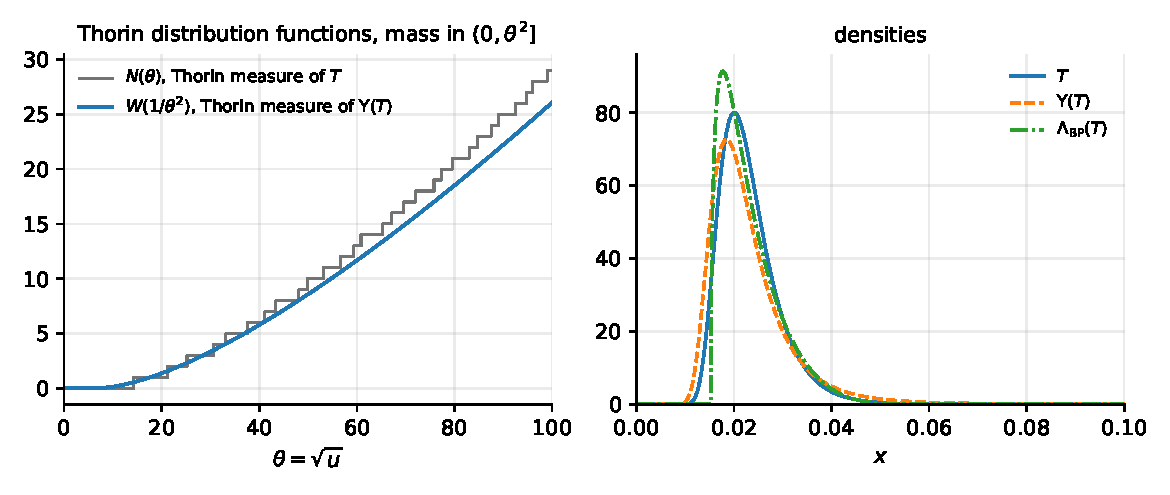
\includegraphics[width=\textwidth]{fig/wigfree_laws.pdf}
\caption{Left: the distribution function $W(\theta^{-2})$ of the Thorin measure of $\Upsilon(T)$ in the chart $\theta=\sqrt u$, against the zero count $N(\theta)$, which under RH is the distribution function of the Thorin measure of $T$ in the same chart. Right: the densities of $T$, of $\Upsilon(T)$ and of $\Lambda_{\rm BP}(T)$ on $[0,0.1]$; the last vanishes to the left of $c=0.0153$. Computed by \texttt{wigfree\_upsilon.py} and drawn by \texttt{wigfree\_plots.py}.}
\label{fig:wigfree:laws}
\end{figure}

\subsection{The semicircle as a local model for the Jacobi parameters}\label{sec:wigfree:jacobi}

Section~\ref{ch:heat} builds from the Stieltjes moments $m_0,\dots,m_{2N-1}$ the Jacobi matrix $J_N$ of the measure $\nu=\sum_ja_j^{-1}\delta_{1/a_j}$, with diagonal entries $\alpha_1,\dots,\alpha_N$ and positive off diagonal entries $\beta_1,\dots,\beta_{N-1}$, the recurrence coefficients of the orthogonal polynomials of $\nu$, computed from the Taylor coefficients of $\Xi$ at the centre alone.

For constant parameters $\alpha_n=\alpha$ and $\beta_n=\beta$ the Jacobi matrix is $\alpha+\beta(S+S^*)$ on $\ell^2(\{0,1,2,\dots\})$, with $S$ the unilateral shift, and the spectral measure of its first basis vector is the semicircle law on $[\alpha-2\beta,\alpha+2\beta]$. The $N\times N$ truncations have the eigenvalues $\alpha+2\beta\cos(\pi k/(N+1))$, $1\le k\le N$, whose distribution tends to the arcsine law with density $\big(\pi\sqrt{4\beta^2-(x-\alpha)^2}\big)^{-1}$ on the same interval, the density of states. If the parameters vary slowly, the eigenvalues are counted by integrating local arcsine laws over the rows. For recurrence coefficients that vary on the scale of the matrix size, $\alpha_{n,N}\to a(n/N)$ and $\beta_{n,N}\to b(n/N)$, this is the theorem of Kuijlaars and Van Assche \cite{KVA99}: the zero distribution of the orthogonal polynomials tends to $\int_0^1\omega_{[a(t)-2b(t),a(t)+2b(t)]}\,dt$, with $\omega_{[A,B]}$ the arcsine law on $[A,B]$. The parameters of $\nu$ decrease to zero with no such scaling, and the count needed below is that of the largest eigenvalues, an edge statement; for $\nu$ the local model is a heuristic. Since $\nu$ has its atoms in $(0,\gamma_1^{-2}]$ and accumulates only at the origin, the local interval $[\alpha_n-2\beta_n,\alpha_n+2\beta_n]$ should reach down to zero, which suggests $\alpha_n\approx2\beta_n$. Write $L(n)=\alpha_n+2\beta_n$ for its right end, taken to decrease in $n$, and $n(L)$ for the inverse function.

The eigenvalues of $J_N$ above a level $x>0$ approximate the atoms $1/\gamma_j^2$ above $x$, of which there are $N(x^{-1/2})$. In the local model row $n$ contributes the mass $\frac2\pi\arccos\sqrt{x/L(n)}$ of the arcsine law on $[0,L(n)]$ above $x$, and nothing when $x\ge L(n)$, so that
\begin{equation}\label{eq:wigfree:count}
N\big(x^{-1/2}\big)=\int_0^\infty\frac2\pi\arccos\sqrt{x/L(n)}_{\,+}\,dn=\frac1\pi\int_x^\infty n(L)\,\frac{\sqrt x\,dL}{L\sqrt{L-x}},
\end{equation}
the second form by an integration by parts in $L$. With $u=1/L$ and $w=1/x$ it becomes Abel's equation
\begin{equation}\label{eq:wigfree:abeleq}
\int_0^w\frac{f(u)\,du}{\sqrt{w-u}}=\pi N(\sqrt w),\qquad f(u)=u^{-1/2}\,n(1/u).
\end{equation}

\begin{proposition}\label{prop:wigfree:abel}
Let $N$ be nondecreasing and right continuous on $[0,\infty)$, with $N=0$ on $[0,\theta_0)$ for some $\theta_0>0$. Then
\begin{equation}\label{eq:wigfree:abel}
n(L)=\int_{(0,L^{-1/2})}\frac{dN(T)}{\sqrt{1-LT^2}}
\end{equation}
gives a locally integrable solution $f$ of \eqref{eq:wigfree:abeleq}, with $N(\sqrt w)$ replaced by its left limit at the jumps of $N$, and it is the only locally integrable solution. If $dN(T)=c\,dT$ on $(0,\infty)$, then $n(L)=\frac\pi2cL^{-1/2}$, so that $L_n=(\pi c/2n)^2$, which is $\gamma_{2n/\pi}^{-2}$ for the ordinates $\gamma_k=k/c$ of that count.
\end{proposition}

\begin{proof}
For $0<a<b$ the substitution $u=1/L$ gives
\begin{align*}
\int_a^b\frac{dL}{L\sqrt{(L-a)(b-L)}}&=\int_{1/b}^{1/a}\frac{du}{\sqrt{(1-au)(bu-1)}}\\
&=\frac1{\sqrt{ab}}\int_{1/b}^{1/a}\frac{du}{\sqrt{(1/a-u)(u-1/b)}}=\frac\pi{\sqrt{ab}} .
\end{align*}
Insert \eqref{eq:wigfree:abel} in the right side of \eqref{eq:wigfree:count}, which is equivalent to \eqref{eq:wigfree:abeleq}, and exchange the integrals, all terms being positive. A point $T$ of the support of $dN$ contributes only when $T<x^{-1/2}$, through $L\in(x,T^{-2})$, and with $b=T^{-2}$ and $\sqrt{1-LT^2}=\sqrt{(b-L)/b}$ its contribution is
\[
\frac{\sqrt x}\pi\int_x^b\frac{\sqrt b\,dL}{L\sqrt{(L-x)(b-L)}}=1 .
\]
So the right side is $N$ of the open interval $(0,x^{-1/2})$, the left limit of $N$ at $x^{-1/2}$. The function $f$ is locally integrable: $n$ vanishes for $L>\theta_0^{-2}$, and for $0<a<b$, by Fubini's theorem, $\int_a^bn(L)\,dL\le\int_{(0,a^{-1/2})}dN(T)\int_0^{T^{-2}}dL/\sqrt{1-LT^2}=2\int_{(0,a^{-1/2})}T^{-2}\,dN(T)<\infty$. If $f_1$ and $f_2$ are two locally integrable solutions, $g=f_1-f_2$ satisfies $\int_0^wg(u)(w-u)^{-1/2}du=0$ for every $w$; integrating against $(y-w)^{-1/2}$ over $w\in(0,y)$ and using $\int_u^y dw/\sqrt{(y-w)(w-u)}=\pi$ gives $\pi\int_0^yg=0$ for every $y$, so $g=0$ almost everywhere. Finally $\int_0^{L^{-1/2}}c\,dT/\sqrt{1-LT^2}=cL^{-1/2}\arcsin1$.
\end{proof}

The local model therefore predicts $\alpha_n\approx2\beta_n\approx\frac12L_n$, with $n(L_n)=n$ \cite{P26wig}. For the zeros of $\xi$ we use the smooth density $dN_0(T)=(2\pi)^{-1}\log(T/2\pi)\,dT$ on $T>2\pi$, for which the substitution $T=L^{-1/2}\sin\varphi$ gives
\[
n(L)=\frac1{2\pi\sqrt L}\int_{\varphi_0}^{\pi/2}\log\frac{\sin\varphi}{2\pi\sqrt L}\,d\varphi,\qquad\sin\varphi_0=2\pi\sqrt L .
\]
As $L\to0$, $\int_0^{\pi/2}\log\sin\varphi\,d\varphi=-\frac\pi2\log2$ gives $n(L)=(4\sqrt L)^{-1}\log(1/(4\pi\sqrt L))+O(1)$, while the rule of Proposition~\ref{prop:wigfree:abel} for a linear count, applied with the ordinates of the smooth count, $N_0(\gamma_r)=r$ with $N_0(T)=(T/2\pi)\log(T/2\pi e)+\frac78$, gives $\frac12L_n=\frac12\gamma_{2n/\pi}^{-2}$ and corresponds to $n=(4\sqrt L)^{-1}\log(1/(2\pi e\sqrt L))$ to the same order. The two rules differ by a factor that tends to one only logarithmically; this is why the cruder rule $\alpha_n\approx\frac12\gamma_{2n/\pi}^{-2}$, which treats the count as linear, is off by a factor near $1.3$.

Table~\ref{tab:wigfree:jacobi} compares the computed parameters with the two rules. The program \texttt{wigfree\_jacobi.py} computes $M_0,\dots,M_{100}$ at $1000$ digits by the trapezoid rule of step $1/600$ on $[0,3.6]$, the moments $m_0,\dots,m_{99}$, and the Cholesky factorisation of $\mathcal H_{50}$. The matrix $L^{-1}[m_{i+j+1}]L^{-\top}$ is tridiagonal to $1.3\times10^{-836}$, and its entries change by at most $2.3\times10^{-429}$ relatively when the factorisation runs at $600$ digits. The first parameters are irregular, $\alpha_1,\dots,\alpha_5=(1.61,3.50,1.80,1.22,1.07)\times10^{-3}$ and $\beta_1,\dots,\beta_5=(1.91,1.15,0.697,0.554,0.498)\times10^{-3}$, and the model is meant for larger $n$. Over $17\le n\le49$ the ratio $\alpha_n/\frac12L_n$ has mean $1.033$ and standard deviation $0.060$ (range $0.940$ to $1.178$), and $2\beta_n/\frac12L_n$ has mean $1.012$ and standard deviation $0.060$ (range $0.893$ to $1.134$); the columns $\alpha_n$, $2\beta_n$, $\frac12L_n$ and these two ratios reproduce Table~6 of \cite{P26wig} to the digits shown there. Over the same range $\alpha_n/(2\beta_n)$ has mean $1.021$ and standard deviation $0.047$, and $\beta_n^2/(\alpha_n\alpha_{n+1})$, which is $\frac14$ in the local model, has mean $0.2502$ and standard deviation $0.013$ (mean $0.256$ and standard deviation $0.059$ over $1\le n\le49$). The cruder rule falls short: $\alpha_n$ and $2\beta_n$ exceed it by the factors $1.286$ and $1.26$ on average, with standard deviations $0.081$ and $0.078$.

Two cautions apply. The rule $n(L_n)=n$ and the midpoint rule $n(L_n')=n-\frac12$ differ by a shift of $n$ of order one, which the asymptotics cannot see, and they move the mean ratios by two per cent, to $1.011$ and $0.991$, within the scatter; the data do not decide between them. And the scatter itself, about six per cent, is not explained by this computation: the note attributes it to the discreteness of the zeros, which the smooth density ignores, and that remains to be tested (Problem~\ref{prob:wigfree:jacobi}). So the local semicircle model predicts the size of the Jacobi parameters to a few per cent over $17\le n\le49$ with no fitted constant, but the agreement is not a proof of an asymptotic law.

\begin{table}[htbp]
\centering\footnotesize
\setlength{\tabcolsep}{2.6pt}
\begin{tabular}{rcccccccccc}
\toprule
 & \multicolumn{3}{c}{$10^5\times$} & \multicolumn{2}{c}{ratio to $\frac12L_n$} & $10^5\times$ & \multicolumn{2}{c}{ratio to $\frac12L_n'$} & $10^5\times$ & \\
\cmidrule(lr){2-4}\cmidrule(lr){5-6}\cmidrule(lr){7-7}\cmidrule(lr){8-9}\cmidrule(lr){10-10}
$n$ & $\alpha_n$ & $2\beta_n$ & $\frac12L_n$ & $\alpha_n$ & $2\beta_n$ & $\frac12L_n'$ & $\alpha_n$ & $2\beta_n$ & $\frac12\gamma_{2n/\pi}^{-2}$ & $\frac{\beta_n^2}{\alpha_n\alpha_{n+1}}$\\
\midrule
5 & 107.3 & 99.54 & 84.84 & 1.27 & 1.17 & 94.11 & 1.14 & 1.06 & 61.8 & 0.2665\\
9 & 56.96 & 51.12 & 45.73 & 1.25 & 1.12 & 48.70 & 1.17 & 1.05 & 34.5 & 0.2548\\
13 & 30.20 & 32.52 & 30.07 & 1.00 & 1.08 & 31.48 & 0.959 & 1.03 & 23.2 & 0.2611\\
17 & 21.71 & 21.51 & 21.83 & 0.995 & 0.986 & 22.64 & 0.959 & 0.950 & 17.0 & 0.2362\\
21 & 18.50 & 16.55 & 16.82 & 1.10 & 0.983 & 17.34 & 1.07 & 0.954 & 13.3 & 0.2479\\
25 & 15.90 & 14.58 & 13.50 & 1.18 & 1.08 & 13.85 & 1.15 & 1.05 & 10.7 & 0.2588\\
29 & 11.25 & 11.45 & 11.16 & 1.01 & 1.03 & 11.41 & 0.986 & 1.00 & 8.93 & 0.2550\\
33 & 9.530 & 9.336 & 9.424 & 1.01 & 0.991 & 9.615 & 0.991 & 0.971 & 7.59 & 0.2647\\
37 & 8.704 & 8.163 & 8.101 & 1.07 & 1.01 & 8.249 & 1.06 & 0.990 & 6.56 & 0.2463\\
41 & 6.998 & 7.053 & 7.062 & 0.991 & 0.999 & 7.179 & 0.975 & 0.982 & 5.74 & 0.2618\\
45 & 6.498 & 6.150 & 6.228 & 1.04 & 0.987 & 6.323 & 1.03 & 0.973 & 5.08 & 0.2481\\
49 & 5.957 & 6.172 & 5.547 & 1.07 & 1.11 & 5.625 & 1.06 & 1.10 & 4.54 & 0.2738\\
\bottomrule
\end{tabular}
\caption{The Jacobi parameters of $\nu$ against the local semicircle model: $\alpha_n$ and $2\beta_n$; half the right end $\frac12L_n$ of the local interval from \eqref{eq:wigfree:abel} with the smooth density and $n(L_n)=n$, and the ratios to it; the same with the midpoint rule $n(L_n')=n-\frac12$; the cruder rule $\frac12\gamma_{2n/\pi}^{-2}$, with $N_0(\gamma_r)=r$; and $\beta_n^2/(\alpha_n\alpha_{n+1})$, which is $\frac14$ in the local model. Computed by \texttt{wigfree\_jacobi.py}.}
\label{tab:wigfree:jacobi}
\end{table}

\subsection{Gamma(2), Laguerre polynomials and finite free convolution}\label{sec:wigfree:gamma2}

Williams' variable \cite{Williams90} $S_2=J+J'=\sum_n\frac2{\pi^2n^2}\Gamma_n$, with independent Gamma(2) variables $\Gamma_n$, the sum of two independent copies of the hitting time $J=\sum_n\frac2{\pi^2n^2}e_n$ of Section~\ref{bp:sec:mellin}, satisfies $2\xi(s)=\E(\frac\pi2S_2)^{s/2}$ \eqref{bp:eq:bpy} \cite{BPY01}, and the RH content of this identity lies on its Mellin side (Theorem~\ref{rz:thm:bpy} and Section~\ref{sec:ch19:williams}). The cumulants of $S_2$ are $\kappa_m=2(m-1)!\,(2/\pi^2)^m\zeta(2m)$.

\begin{proposition}\label{prop:wigfree:s1}
For every complex $s$,
\begin{equation}\label{eq:wigfree:s1}
\E\Big[\Big(\frac\pi2J\Big)^{s/2}\Big]=\frac{2(1-2^{1-s})\,\xi(s)}{s-1}=s\,\pi^{-s/2}\,\Gamma\Big(\frac s2\Big)(1-2^{1-s})\,\zeta(s),
\end{equation}
the value at $s=1$ being $2\xi(1)\log2=\log2$. Equivalently $J\stackrel d=V^{-2}S_2$, with $V$ uniform on $[1,2]$ and independent of $S_2$. The function \eqref{eq:wigfree:s1} vanishes at the zeros of $\xi$ and at the points $1+2\pi ik/\log2$, $k\ne0$, of the line $\re s=1$, and, unlike the zero set of $\xi$, its zero set is not symmetric under $s\mapsto1-s$.
\end{proposition}

\begin{proof}
This is the multiplicative relation of Biane, Pitman and Yor between $J$, their $\Sigma_1$, and $S_2$, their $\Sigma_2$ \cite[Table 1 and (43) to (45)]{BPY01}; we give the computation. For $\re p<0$, $\int_0^\infty\lambda^{-p-1}e^{-\lambda x}d\lambda=\Gamma(-p)x^p$ and $\E e^{-\lambda J}=\sqrt{2\lambda}/\sinh\sqrt{2\lambda}$ give, with $r=\sqrt{2\lambda}$,
\[
\E J^p=\frac{2^{p+1}}{\Gamma(-p)}\int_0^\infty\frac{r^{-2p}}{\sinh r}\,dr=\frac{2^{p+2}(1-2^{2p-1})\,\Gamma(1-2p)\,\zeta(1-2p)}{\Gamma(-p)},
\]
by $1/\sinh r=2\sum_{k\ge0}e^{-(2k+1)r}$, which gives $\int_0^\infty r^{z-1}/\sinh r\,dr=2(1-2^{-z})\Gamma(z)\zeta(z)$ for $\re z>1$. Put $p=s/2$ with $\re s<0$. The functional equation $\zeta(1-s)=\pi^{1/2-s}\Gamma(\frac s2)\zeta(s)/\Gamma(\frac{1-s}2)$, the duplication formula $\Gamma(1-s)=2^{-s}\pi^{-1/2}\Gamma(\frac{1-s}2)\Gamma(1-\frac s2)$ and $\Gamma(1-\frac s2)/\Gamma(-\frac s2)=-\frac s2$ turn this into $\E J^{s/2}=-2^{1-s/2}s(1-2^{s-1})\pi^{-s}\Gamma(\frac s2)\zeta(s)$, and multiplying by $(\pi/2)^{s/2}$ gives \eqref{eq:wigfree:s1}. Both sides are entire, since $J$ has moments of all real orders and the zero of $1-2^{1-s}$ at $s=1$ cancels the pole of $\zeta$, so the identity holds for every $s$. Since $\E V^{-s}=\int_1^2v^{-s}dv=(1-2^{1-s})/(s-1)$, the right side is $\E V^{-s}\,\E(\frac\pi2S_2)^{s/2}$. The factor $1-2^{1-s}$ vanishes exactly at $1+2\pi ik/\log2$; on the line $\re s=0$, the image of $\re s=1$ under $s\mapsto1-s$, it equals $-1$ at the corresponding points $2\pi ik/\log2$ and $\xi$ has no zeros, so the zero set is not symmetric.
\end{proof}

The elementary factor $(1-2^{1-s})/(s-1)$ adds zeros on the line $\re s=1$, the first at height $2\pi/\log2=9.0647$, the zeros of the alternating zeta function that Section~\ref{wr:sec:salem} meets.

\begin{proposition}\label{prop:wigfree:wishart}
Let $z_1,z_2,\dots$ be independent standard complex Gaussian vectors in $\C^2$, with $\E z_nz_n^*=I_2$, let $c_n=2/(\pi^2n^2)$ and $W=\sum_nc_nz_nz_n^*$. Then $\operatorname{tr}W\stackrel d=S_2$, so that $2\xi(s)=\E(\frac\pi2\operatorname{tr}W)^{s/2}$, and
\[
\E\det(x-W)=x^2-2m_1x+m_1^2-m_2,\qquad m_k=\sum_nc_n^k,\quad m_1=\tfrac13,\ m_2=\tfrac2{45},
\]
with the real roots $m_1\pm\sqrt{m_2}=0.122515$ and $0.544152$. This is the finite free convolution $\boxplus_2$ of the polynomials $\E\det(x-c_nz_nz_n^*)=x(x-2c_n)$, and the mixed characteristic polynomial of Marcus, Spielman and Srivastava \cite{MSS15} of the matrices $c_nI_2$.
\end{proposition}

\begin{proof}
$|z_n|^2$ is the sum of two independent standard exponential variables, so $\operatorname{tr}W=\sum_nc_n|z_n|^2\stackrel d=S_2$. For a $2\times2$ matrix, $\det(x-W)=x^2-x\operatorname{tr}W+\det W$ and $\det W=\frac12((\operatorname{tr}W)^2-\operatorname{tr}W^2)$. Here $\E\operatorname{tr}W=2m_1$ and $\E(\operatorname{tr}W)^2=\operatorname{Var}S_2+(\E S_2)^2=2m_2+4m_1^2$, while $\E\operatorname{tr}W^2=\sum_{n,k}c_nc_k\E|z_n^*z_k|^2=6m_2+2(m_1^2-m_2)$, since $\E|z_n|^4=6$ and $\E|z_n^*z_k|^2=\operatorname{tr}(I_2I_2)=2$ for $n\ne k$. Hence $\E\det W=m_1^2-m_2$. The terms $c_nz_nz_n^*$ are independent and unitarily invariant in law, with $\E\det(x-c_nz_nz_n^*)=x^2-2c_nx$, so by \cite[Theorem 1.2]{MSS22} and bilinearity the expected characteristic polynomial of a finite partial sum is the $\boxplus_2$ convolution of these polynomials; with the coefficient formula of $\boxplus_2$, adding $x(x-2c)$ to a polynomial $x^2-Ax+B$ gives $x^2-(A+2c)x+B+Ac$, so the constant term is $2\sum_{n<k}c_nc_k=m_1^2-m_2$ in the limit.
\end{proof}

The reading of the exponent two of $(\sqrt{2\lambda}/\sinh\sqrt{2\lambda})^2$ as the size of the matrix is special to the sinh family of \cite{BPY01}.

In the normalisation of \cite{MSS22} write a polynomial of degree $d$ as $p(x)=\sum_k(-1)^k\binom dke_kx^{d-k}$; the multiplicative convolution $\boxtimes_d$ multiplies the normalised coefficients, $e_k(p\boxtimes_dq)=e_k(p)e_k(q)$ \cite[Definition 1.4]{MSS22}, and by Szeg\H{o}'s theorem it preserves the property of having only nonnegative roots \cite[Theorem 1.6]{MSS22}.

\begin{lemma}\label{lem:wigfree:laguerre}
Let $a>0$ and $(a)_k=a(a+1)\cdots(a+k-1)$.
\begin{enumerate}
\item[(i)] The reversed Laguerre polynomial $q_a(x)=x^dL_d^{(a-1)}(1/x)$ has $d$ positive simple roots and normalised coefficients $e_k=e_0/(a)_k$, $e_0=\Gamma(d+a)/(d!\,\Gamma(a))$. Hence $p\boxtimes_d(q_a/e_0)$ has the normalised coefficients $e_k(p)/(a)_k$, and it has only real roots whenever the roots of $p$ are real and of one sign.
\item[(ii)] $\{1/(a)_k\}_{k\ge0}$ is a multiplier sequence: the function
\[
\sum_k\frac{x^k}{k!\,(a)_k}=\Gamma(a)x^{(1-a)/2}I_{a-1}(2\sqrt x)
\]
is entire of order $\frac12$ with only real negative zeros, at $-j_{a-1,m}^2/4$.
\item[(iii)] A density $f$ on $(0,\infty)$ is a scale mixture of Gamma$(a)$ densities if and only if $x^{1-a}f(x)$ is completely monotone; for $a=2$, if and only if $f(x)/x$ is.
\end{enumerate}
\end{lemma}

\begin{proof}
(i) By \cite[(18.5.12)]{DLMF},
\[
x^dL_d^{(a-1)}(1/x)=\sum_k(-1)^k\binom{d+a-1}{d-k}\frac{x^{d-k}}{k!},
\]
and $\binom{d+a-1}{d-k}/(k!\binom dk)=\Gamma(d+a)/(d!\,\Gamma(k+a))$, which is $e_0/(a)_k$. The zeros of $L_d^{(a-1)}$ are positive and simple, those of an orthogonal polynomial for the weight $x^{a-1}e^{-x}$ on $(0,\infty)$ \cite[Section 18.2(vi)]{DLMF}, and the roots of $q_a$ are their reciprocals. The statement on $\boxtimes_d$ is Szeg\H{o}'s theorem for roots of one sign; for nonpositive roots apply it to $(-1)^dp(-x)$, whose normalised coefficients are $(-1)^ke_k(p)$. (ii) The series is that of the modified Bessel function \cite[(10.25.2)]{DLMF}. For $x=-y^2/4<0$ it equals $\Gamma(a)(y/2)^{1-a}J_{a-1}(y)$, and for $a-1>-1$ the zeros of $J_{a-1}(y)/y^{a-1}$ are real \cite[Section 10.21(i)]{DLMF}. A real entire function of order less than one with only real zeros is in the Laguerre P\'olya class, and by the theorem of P\'olya and Schur \cite{PS14} a sequence whose exponential generating function is in that class with coefficients of one sign is a multiplier sequence. (iii) $f(x)=\int_0^\infty\theta^{-a}x^{a-1}e^{-x/\theta}\,\varpi(d\theta)/\Gamma(a)$ says that $x^{1-a}f(x)$ is the Laplace transform of a positive measure in the variable $1/\theta$; conversely Bernstein's theorem writes a completely monotone $x^{1-a}f(x)$ in this form.
\end{proof}

Let $X$ be the P\'olya variable, with density $p=\Phi/\Xi(0)$ for the kernel $\Phi$ of \eqref{eq:ch2:Phi} and moment generating function $\E e^{sX}=G(s^2)$ \eqref{eq:ch2:mgf}, and write $G(u)=\sum_kb_ku^k$, so that $b_k=\E X^{2k}/(2k)!=M_k/((2k)!\,M_0)$ with $M_k=\int_\R v^{2k}\Phi(v)\,dv$, as in Sections~\ref{ch:heat} and~\ref{fm:sec:polyanec}.

\begin{proposition}\label{prop:wigfree:peel}
For $a>0$ let $G_a(u)=\sum_kb_ku^k/(a)_k$. If RH holds, then for every $a>0$ the function $G_a$ is in the Laguerre P\'olya class with only real negative zeros, and all its Jensen polynomials $\sum_{i=0}^d\binom di(n+i)!\,b_{n+i}x^i/(a)_{n+i}$, $d,n\ge0$, have only real negative zeros. Multiplying the coefficients by $(a)_k$ instead does not preserve real zeros: it turns $(1+u)^2=1+2u+u^2$ into $1+2au+a(a+1)u^2$, whose discriminant is $-4a<0$.
\end{proposition}

\begin{proof}
Under RH, $G(u)=\prod_j(1+u/\gamma_j^2)$ with $\sum_j\gamma_j^{-2}<\infty$, so $G$ is in the Laguerre P\'olya class, and by P\'olya's theorem its Jensen polynomials $J_{d,n}(x)=\sum_i\binom di(n+i)!\,b_{n+i}x^i$ of Section~\ref{fm:sec:polyanec} have only real zeros. Since $(a)_{n+i}=(a)_n(a+n)_i$, the Jensen polynomial of $G_a$ of degree $d$ and shift $n$ is $1/(a)_n$ times the image of $J_{d,n}$ under the multiplier sequence $\{1/(a+n)_i\}_i$ of Lemma~\ref{lem:wigfree:laguerre}(ii), so it has only real zeros, negative because its coefficients are positive. For $n=0$, $\binom di\,i!\,d^{-i}\to1$ gives $\sum_i\binom di\,i!\,b_ix^i/((a)_id^i)\to G_a(x)$ uniformly on compact sets as $d\to\infty$, so by Hurwitz's theorem $G_a$ has only real negative zeros; since $(a)_k\ge a(k-1)!$, $G_a$ has order at most $\frac13$, and it is in the Laguerre P\'olya class. The example is a direct computation.
\end{proof}

In terms of Lemma~\ref{lem:wigfree:laguerre}(i), dividing the normalised coefficients by $(a)_k$ is the multiplicative convolution with $q_a/e_0$, so peeling a Gamma($a$) layer, the operation that would pass from the moments of a Gamma($a$) scale mixture to those of its mixing law, keeps zeros real, while the inverse operation can destroy them. The note calls the peeling a free Poisson operation. The example does not show that no argument could pass from real zeros of some $G_a$ to real zeros of $G$, as the note puts it.

Lemma~\ref{lem:wigfree:laguerre}(iii) makes the Gamma(2) mixture route of \cite[Section 12.6]{P26}, which Section~\ref{sec:ch19:williams} recalls as excluded, a statement about complete monotonicity.

\begin{theorem}\label{thm:wigfree:nomix}
For no $a>0$ is $|X|$, $X^2$ or $S_2$ a scale mixture of Gamma$(a)$ laws.
\end{theorem}

\begin{proof}
By Lemma~\ref{lem:wigfree:laguerre}(iii) a mixture would make $g(x)=x^{1-a}f(x)$ completely monotone, with $f$ the density. A completely monotone $g\not\equiv0$ is positive and log convex, so $g(x)\ge g(1)\exp\big((x-1)g'(1)/g(1)\big)$ for $x\ge1$: it decays at most exponentially. For $v\ge0$, dropping the negative terms of \eqref{eq:ch2:Phi} and using $e^{2v}\ge1$ gives
\[
\Phi(v)\le4\pi^2e^{9v/2}\exp(-\pi e^{2v})\sum_{n\ge1}n^4e^{-\pi(n^2-1)},
\]
a constant multiple of $e^{9v/2}\exp(-\pi e^{2v})$. The densities of $|X|$ and $X^2$ are $2\Phi(v)/\Xi(0)$ and $\Phi(\sqrt w)/(\Xi(0)\sqrt w)$, so $v^{1-a}\Phi(v)$ and $w^{1/2-a}\Phi(\sqrt w)$ would have to be completely monotone, and both decay faster than any exponential. For $S_2$ the obstruction is at the origin. By Chebyshev's inequality in exponential form, for $\lambda>0$, $\Pr(S_2\le x)\le e^{\lambda x}\E e^{-\lambda S_2}=e^{\lambda x}\big(\sqrt{2\lambda}/\sinh\sqrt{2\lambda}\big)^2$, and $\lambda=2/x^2$ gives
\[
\Pr(S_2\le x)\le\frac{16\,e^{-2/x}}{x^2(1-e^{-4/x})^2}\le17\,x^{-2}e^{-2/x},\qquad0<x\le1 .
\]
A mixture would give, $g$ being nonincreasing and $g(1)>0$, $f(x)\ge g(1)x^{a-1}$ and $\Pr(S_2\le x)\ge g(1)x^a/a$ for $0<x\le1$, which is impossible as $x\downarrow0$.
\end{proof}

The Hankel test sees the failure at low order. If $Y=\Theta\,\Gamma$ with $\Gamma$ a Gamma$(a)$ variable independent of $\Theta\ge0$, then $\E Y^k=(a)_k\E\Theta^k$, so $\mu_k=\E Y^k/(a)_k$ must be a Stieltjes moment sequence, and both $[\mu_{i+j}]_{i,j<N}$ and $[\mu_{i+j+1}]_{i,j<N}$ must be positive semidefinite for every $N$. Table~\ref{tab:wigfree:hankel} gives the least order $N$ at which each fails to be positive definite, by Cholesky factorisation at $400$ digits, with the same orders at $250$. The moments of $X^2$ are $M_k/M_0$; those of $|X|$ come from a tanh sinh rule, since odd powers of $|v|$ are not smooth at the origin; those of $S_2$ follow from its cumulants. The table of \cite{P26wig} is the Hamburger row, the first matrix alone.

\begin{table}[htbp]
\centering\footnotesize
\setlength{\tabcolsep}{4pt}
\begin{tabular}{lccccccccccc}
\toprule
$a$ & $\frac12$ & $1$ & $\frac32$ & $2$ & $\frac52$ & $3$ & $4$ & $6$ & $8$ & $12$ & $20$\\
\midrule
$|X|$, Stieltjes & 2 & 2 & 2 & 2 & 2 & 3 & 3 & 3 & 4 & 4 & 5\\
$|X|$, Hamburger & 2 & 2 & 2 & 3 & 3 & 3 & 3 & 4 & 4 & 5 & 6\\
$X^2$, Stieltjes & 2 & 3 & 3 & 4 & 4 & 4 & 5 & 5 & 6 & 7 & 9\\
$X^2$, Hamburger & 2 & 3 & 4 & 4 & 4 & 5 & 5 & 6 & 6 & 7 & 9\\
$S_2$, both & 2 & 2 & 2 & 2 & 2 & 2 & 2 & 3 & 4 & 6 & 12\\
\bottomrule
\end{tabular}
\caption{The first order $N$ at which the moments $\mu_k=\E Y^k/(a)_k$ fail the Hankel test for a Gamma$(a)$ scale mixture, for $Y=|X|$, $X^2$ and $S_2$: the Hamburger test uses $[\mu_{i+j}]_{i,j<N}$ alone, the Stieltjes test also $[\mu_{i+j+1}]_{i,j<N}$. Computed by \texttt{wigfree\_gamma2.py}.}
\label{tab:wigfree:hankel}
\end{table}

The theorem also settles which tool applies. Kristiansen proved Steutel's conjecture that scale mixtures of Gamma(2) laws are infinitely divisible \cite{Kristiansen94}; since $x^{\alpha-2}e^{-x}$ is completely monotone for $\alpha\le2$, Lemma~\ref{lem:wigfree:laguerre}(iii) makes Gamma$(\alpha)$ itself a scale mixture of Gamma(2) laws, and the theorem covers scale mixtures of Gamma$(\alpha)$ laws for every $\alpha\le2$. By Theorem~\ref{thm:wigfree:nomix} it cannot be applied to $|X|$, $X^2$ or $S_2$. The Gamma(2) structure that is true is Williams' convolution, a GGC and hence infinitely divisible directly.

\subsection{The heat flow and finite free convolution}\label{sec:wigfree:heat}

Remark~\ref{rem:wigbiane:direction} identifies the forward heat flow on polynomials with finite free convolution by a Hermite polynomial and, as the degree grows, with free convolution by a semicircle law. The time is the variance of the semicircle law. For a real polynomial $p$ of degree $d\ge2$ write $p_t=e^{-(t/2)D^2}p$, a finite sum, and
\[
q_t(x)=e^{-(t/2)D^2}x^d=t^{d/2}H_d\big(x/\sqrt t\big),\qquad t>0,
\]
with $q_0=x^d$ and $H_d=e^{-D^2/2}x^d$ the Hermite polynomial of Remark~\ref{rem:wigbiane:direction}, whose zeros are real. The time $t$ is twice the time of Section~\ref{sec:ch21:flow}, where $\partial_tH_t=-\partial_z^2H_t$.

\begin{proposition}\label{prop:wigfree:heat}
Let $p$ be a real polynomial of degree $d\ge2$ and $s,t\ge0$.
\begin{enumerate}
\item[(i)] $p_t=p\boxplus_dq_t$.
\item[(ii)] $q_s\boxplus_dq_t=q_{s+t}$.
\item[(iii)] If $p$ has only real roots, then so has $p_t$, and the largest root of $p_t$ is at most the largest root of $p$ plus $\sqrt t\,h_d$, where $h_d$ is the largest zero of $H_d$.
\item[(iv)] While the roots $z_1(t),\dots,z_d(t)$ of $p_t$ are simple, $\dot z_k=\sum_{j\ne k}(z_k-z_j)^{-1}$.
\end{enumerate}
\end{proposition}

\begin{proof}
(i) In operator form, $p\boxplus_dq=\hat p(D)\hat q(D)x^d$ when $p=\hat p(D)x^d$ and $q=\hat q(D)x^d$ \cite[Definition 1.1 and (2)]{MSS22}. For $q=q_t$ the operator $\hat q(D)$ acts on polynomials of degree at most $d$ as $e^{-(t/2)D^2}$, and operators in $D$ commute, so $p\boxplus_dq_t=e^{-(t/2)D^2}\hat p(D)x^d=p_t$. (ii) is (i) for $p=q_s$, since $e^{-(t/2)D^2}e^{-(s/2)D^2}=e^{-((s+t)/2)D^2}$; it is the identity $a^dH_d(x/a)\boxplus_db^dH_d(x/b)=c^dH_d(x/c)$, $c^2=a^2+b^2$, of \cite[Section 1.2]{MSS22}. (iii) The roots of $q_t$ are $\sqrt t$ times those of $H_d$, and by Walsh's theorem \cite[Theorem 1.3]{MSS22} the convolution $p\boxplus_dq$ of two polynomials of degree $d$ with only real roots has only real roots, the largest at most the sum of the largest roots of $p$ and $q$. (iv) Differentiate $p_t(z_k(t))=0$ in $t$ and use $\partial_tp_t=-\frac12p_t''$: $\dot z_k=\frac12p_t''(z_k)/p_t'(z_k)$. Writing $p_t=(x-z_k)r$ gives $p_t'(z_k)=r(z_k)$ and $p_t''(z_k)=2r'(z_k)$, so that $\dot z_k=r'(z_k)/r(z_k)=\sum_{j\ne k}(z_k-z_j)^{-1}$.
\end{proof}

For a conjugate pair $x\pm iy$, $y>0$, the partner contributes $-1/(2y)$ to $\dot y$, and each real root $r$ contributes $\im(x+iy-r)^{-1}=-y/((x-r)^2+y^2)<0$: the pair is drawn to the axis by its partner and pulled further by every real root. On its own, $(x-1)^2+0.64$ becomes $(x-1)^2+0.64-t$, which reaches the axis at $t=0.64$. The example of the note adds four real roots,
\[
p(x)=(x+3)(x+1)\big(x-\tfrac12\big)(x-2)\big((x-1)^2+0.64\big).
\]
The discriminant of $p_t$ in $x$ is a polynomial of degree $15$ in $t$ whose only root in $(0,2)$ is $t^*=0.3203291143987806$. Before $t^*$ the roots are distinct, so the pair stays off the axis, and since $p_t=e^{-((t-t^*)/2)D^2}p_{t^*}$ for $t>t^*$, part (iii) keeps all roots real afterwards: the pair meets the axis at $t^*$, at the point $1.25743$, in about half the time it needs on its own. The program \texttt{wigfree\_heat.py} computes the discriminant exactly.

\begin{figure}[htbp]
\centering
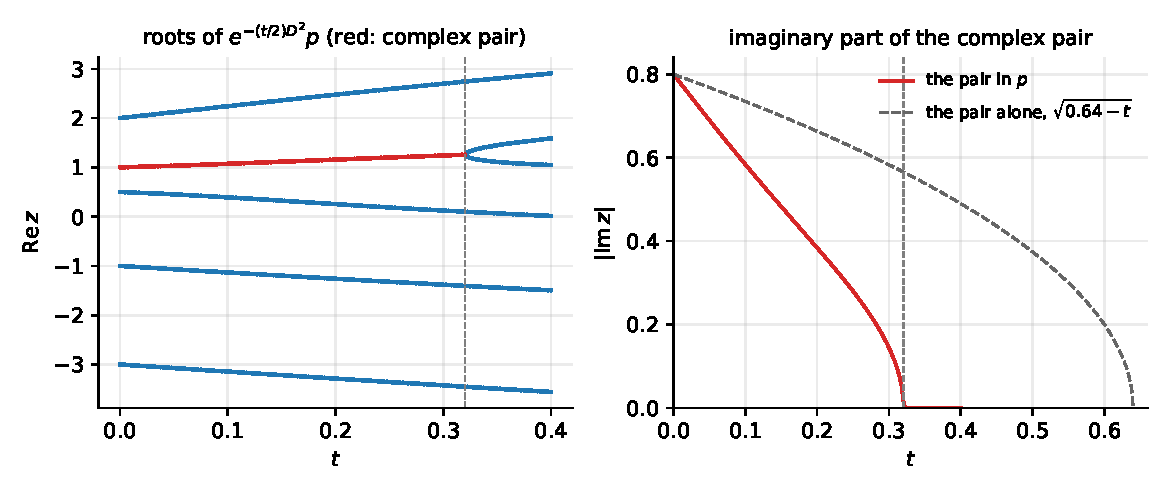
\includegraphics[width=\textwidth]{fig/wigfree_heat.pdf}
\caption{The flow $e^{-(t/2)D^2}p$ for $p$ with the roots $-3$, $-1$, $\frac12$, $2$ and $1\pm0.8i$. Left: the real parts of the six roots for $0\le t\le0.4$; the complex pair has one real part until it meets the axis at $t^*=0.3203$ (dashed), where its two roots split. Right: the imaginary part of the pair, against $\sqrt{0.64-t}$ for the pair on its own, which reaches the axis at $t=0.64$. Computed by \texttt{wigfree\_heat.py} and drawn by \texttt{wigfree\_plots.py}.}
\label{fig:wigfree:heat}
\end{figure}

The Hermite polynomial is the finite free counterpart of the semicircle law: $H_d$ is the expected characteristic polynomial of a symmetric Gaussian matrix \cite[Section 1.2]{MSS22}, and the roots of $H_d(\sqrt d\,x)$, the roots of $q_{1/d}$, are close to the quantiles $x_k$ of $\sigma_1$ given by $\sigma_1([-2,x_k])=(k-\frac12)/d$. The largest deviation from the quantiles is at the edge, and its products with $d^{2/3}$, from $0.3906$ to $0.4962$ for $d=20$ to $320$, grow slowly, as they should at the edge scale $d^{-2/3}$ of the extreme zeros. In the limit $d\to\infty$ finite free convolution becomes free convolution \cite{AP18}, \cite[Section 1.2]{MSS22}: if the root distributions of polynomials $p_d$ with only real roots tend to a law $\mu$ in moments, those of $p_d\boxplus_dq_{t/d}$ tend to $\mu\boxplus\sigma_t$.

For $H_t$ the identification is a heuristic. The motion of the zeros is the same, up to the factor two in the time (Section~\ref{sec:ch21:flow}), but $H_t$ has infinitely many zeros, with a density that grows logarithmically, while the limit theorem concerns the distribution of all $d$ roots of a polynomial after scaling; for $H_t$ it would have to be applied to windows of zeros, with the zeros outside a window acting as an external field, and no theorem of this kind is known. De Bruijn's theorem that real zeros of $H_t$ stay real forward in time \cite{deBruijn} is the counterpart of (iii), proved directly. In Thorin terms the forward flow is the path of clocks $R_t$ of Section~\ref{sec:ch21:flow}, in the time of $H_t$ (Theorem~\ref{rz:thm:dbn}).

The Jensen polynomials of Section~\ref{fm:sec:polyanec} meet the Hermite polynomials directly. Griffin, Ono, Rolen and Zagier proved that for each degree $d$ the Jensen polynomials $J_{d,n}$, after an affine change of variable and a normalisation depending on $n$, tend to the Hermite polynomial of degree $d$ as $n\to\infty$, and this is how they obtain real zeros for all large shifts \cite{GORZ19}. In the language of this subsection the Jensen polynomials of large shift are asymptotically finite free Gaussian; Problem~\ref{prob:wigfree:jensen} asks for an exact finite free structure at every shift.

These limits see the zeros only through their distribution. Moving $o(d)$ of the $d$ roots changes no limit law, so a single nonreal pair is invisible to free convolution limits, and these limits cannot decide RH by themselves \cite{P26wig}.

\section{The Dedekind eta analogue at the basepoint one}\label{ch:bpeta}

At the basepoint one the pole of $\zeta$ and the primes act together: the pole term and the prime atoms of the L\'evy form both have infinite mass on $(1,\infty)$, the form converges only as a compensated limit, and quasi infinite divisibility is lost (Section~\ref{sb:sec:qid}). The $L$ function of the real character $\chi_{12}$ modulo $12$, to which Section~\ref{ch:chi12} carried the pipeline of the book, has no pole. Its completed function is entire and is a Mellin transform of the Dedekind eta function, whose product formula makes the kernel positive, and at the basepoint two its sine squared decomposition loses the pole piece while the prime weights take both signs (Section~\ref{sec:ch16:sin2}). We repeat for $L(s,\chi_{12})$ the calculations that Chapter~\ref{chap:basepoint} made for $\zeta$ at the basepoint one: the Thorin measure and the tail of the shifted clock (Section~\ref{bp:eta:sec}); the L\'evy form, its conversion by the sine squared lemma and its extension below the basepoint one, together with the question of Section~\ref{ch:sato} whether the tilted variable is quasi infinitely divisible (Section~\ref{bp:eta:sec:levy}); and the hitting time with its exact Brownian boundary (Section~\ref{bp:eta:sec:hit}). Together they redraw for $L(s,\chi_{12})$ the part of the map of Section~\ref{pm:sec:map} at the basepoint one.

Every step goes through with the same structure, and the constants change only through the denser zeros. The comparison of the two examples in Section~\ref{bp:sec:compare} therefore separates what in the example of $\zeta$ comes from the pole from what comes from the zeros, and it shows that removing the pole does not move the boundary of what is proved. The scripts are in the folder \texttt{basepoint\_one/eta} of the archive, and we name them at each table and figure.

\subsection{The completed \texorpdfstring{$L$}{L} function and its Thorin measure}\label{bp:eta:sec}

We use the completed function $\xi(s,\chi_{12})=(12/\pi)^{s/2}\Gamma(s/2)L(s,\chi_{12})$, its kernel $K$ and the variable $Y$ with density $K/\xi(\frac12,\chi_{12})$ of Section~\ref{sec:ch16:eta}; the function satisfies $\xi(s,\chi_{12})=\xi(1-s,\chi_{12})$ and is entire as it stands, with no factor like the $\frac12s(s-1)$ of $\xi$: $L(s,\chi_{12})$ has no pole to remove. We computed its zeros on the critical line by sign changes of $\xi(\frac12+it,\chi_{12})e^{\pi t/4}$ with \texttt{zeros12.py}, finding $297$ below height $340$; Section~\ref{sec:ch16:eta} lists the first of them. In this section $b_\alpha=(\xi'/\xi)(\alpha,\chi_{12})$ and $v_\alpha(\theta)=\re(\xi'/\xi)(\alpha+i\theta,\chi_{12})$, and $\varphi_\alpha$, $T_1$, $\widetilde T$, $\Pi$, $A$, $A_\alpha$, $Q$ and $a_k=-(\rho_k-\frac12)^2$ are formed with $\xi(s,\chi_{12})$ and its zeros $\rho=\beta+i\gamma$ in place of $\xi$. So is the tilted eta variable $V_\alpha$, the Esscher tilt of $Y$ by $e^{(\alpha-\frac12)Y}$, with $\E e^{sV_\alpha}=\xi(\alpha+s,\chi_{12})/\xi(\alpha,\chi_{12})$. The constants we need, computed by \texttt{base.py}, are
\[
L(1,\chi_{12})=\frac{\log(2+\sqrt3)}{\sqrt3}=0.760346,\qquad L'(1,\chi_{12})=0.362495,
\]
\[
b_1=\frac{\xi'}{\xi}(1,\chi_{12})=\frac12\log\frac{12}\pi+\frac12\psi\Big(\frac12\Big)+\frac{L'}{L}(1,\chi_{12})=\sum_\rho\frac1\rho=0.1650833123,
\]
where $\psi$ is the digamma function; $b_1$ is about seven times the value for $\zeta$. The Taylor coefficients of $\xi(\frac12+s,\chi_{12})/\xi(\frac12,\chi_{12})$ give the power sums $p_1=\sum_ka_k^{-1}=0.1664618$ and $p_2=\sum_ka_k^{-2}=0.0055985$, which are $\sum_{\gamma>0}\gamma^{-2}$ and $\sum_{\gamma>0}\gamma^{-4}$ under GRH; $p_1$ is the mean of the centre clock.

\label{bp:eta:sec:thorin}At the basepoint one the Thorin measure is positive with no hypothesis, exactly as for $\zeta$ in Proposition~\ref{bp:prop:thorin}, and it tracks the zero count in the same way.

\begin{proposition}\label{bp:eta:prop:thorin}
The function $\varphi_1(u)=\xi(1,\chi_{12})/\xi(1+\sqrt u,\chi_{12})$ is the Laplace transform of a GGC with no drift, with Thorin density in $\theta=\sqrt z$
\[
\frac1\pi v_1(\theta)=\frac1\pi\re\frac{\xi'}{\xi}(1+i\theta,\chi_{12})=\frac1\pi\sum_\rho\frac{1-\beta}{(1-\beta)^2+(\theta-\gamma)^2}>0,
\]
the sum over the nontrivial zeros $\rho=\beta+i\gamma$ of $L(s,\chi_{12})$ in conjugate pairs. Positivity is unconditional because $L(1+it,\chi_{12})\ne0$.
\end{proposition}

\begin{proof}
The proof is that of Proposition~\ref{bp:prop:thorin}, with the Hadamard product of the entire function $\xi(s,\chi_{12})$ in place of that of $\xi$.
\end{proof}

The minimum on $[0,60]$ is at the origin, $v_1(0)/\pi=b_1/\pi=0.0525477$, and the cumulative mass tracks the zero count: $\int_0^{60}v_1/\pi=35.81$ against $N_{\chi_{12}}(60)=36$, where $N_{\chi_{12}}(T)$ counts the zeros with $0<\gamma\le T$ as in Section~\ref{sec:ch16:eta}. Table~\ref{bp:eta:tab:rho}, computed by \texttt{base.py}, compares direct values with the Poisson sum over the $297$ computed zeros; the nearly constant difference of $1.11\times10^{-3}$ is the contribution of the zeros above height $340$. Figure~\ref{bp:eta:fig:density} compares the density with that of $\zeta$: on this window the zeros of $L(s,\chi_{12})$ are more than twice as dense, and its density is correspondingly higher. As for $\zeta$, $\varphi_1(u)=1-b_1\sqrt u+O(u)$, so $T_1$ has infinite mean and $P(T_1>x)\sim b_1(\pi x)^{-1/2}=0.09314\,x^{-1/2}$.

\begin{table}[htbp]
\centering\small
\begin{tabular}{rcc}
\toprule
$\theta$ & $v_1(\theta)/\pi$ from $\xi'/\xi(\cdot,\chi_{12})$ & from 297 zeros, $\beta=\frac12$\\
\midrule
0 & 0.0525477 & 0.0514359\\
3.8046276 & 0.6889076 & 0.6877958\\
5 & 0.1852757 & 0.1841637\\
10 & 0.2694467 & 0.2683341\\
30 & 0.7445558 & 0.7434362\\
60 & 0.7298854 & 0.7287413\\
\bottomrule
\end{tabular}
\caption{The Thorin density $v_1/\pi$ of $\xi(1,\chi_{12})/\xi(1+\sqrt u,\chi_{12})$, computed from $\xi'/\xi(\cdot,\chi_{12})$ and from the Poisson sum over the $297$ zeros of $L(s,\chi_{12})$ below height $340$ with $\beta=\frac12$; the difference is the contribution of the zeros above height $340$.}
\label{bp:eta:tab:rho}
\end{table}

\begin{figure}[htbp]
\centering
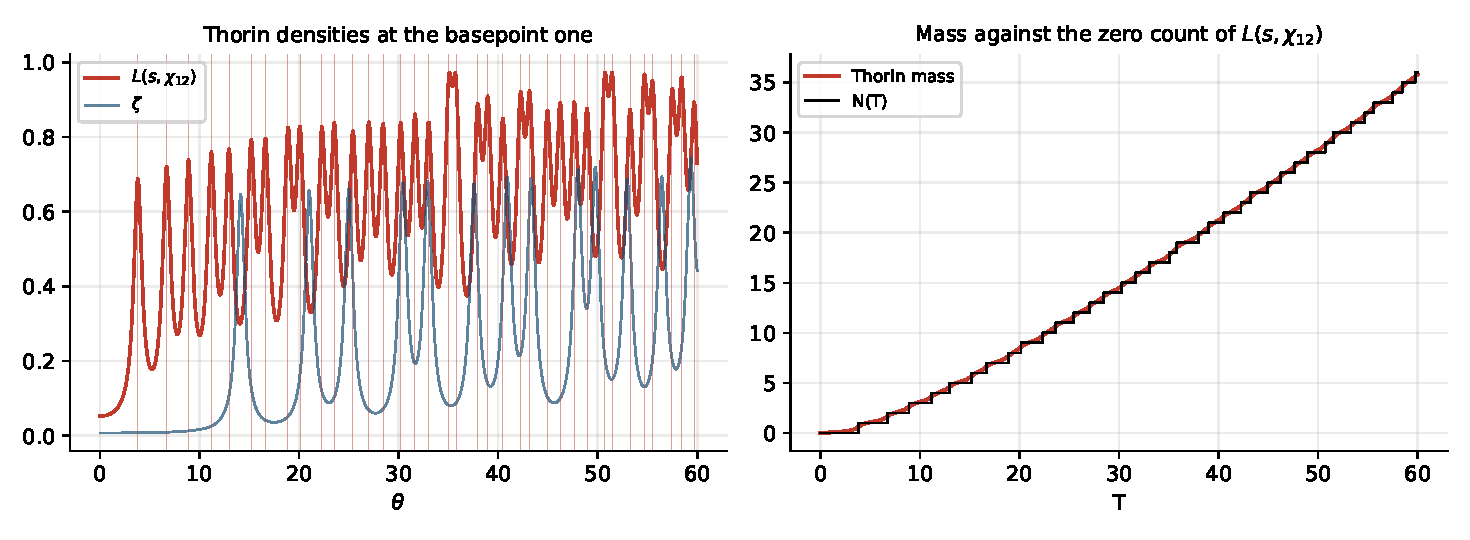
\includegraphics[width=\textwidth]{fig/bp1eta_density.pdf}
\caption{Left: the Thorin densities at the basepoint one for $L(s,\chi_{12})$ and for $\zeta$ on $[0,60]$, with the ordinates of the zeros of $L(s,\chi_{12})$ (vertical lines). Right: the cumulative Thorin mass for $L(s,\chi_{12})$ against its zero count $N_{\chi_{12}}(T)$, written $N(T)$ in the plot. Drawn by \texttt{figs.py} of \texttt{basepoint\_one/eta}.}
\label{bp:eta:fig:density}
\end{figure}

\subsection{The L\'evy form without a pole, at and below the basepoint one}\label{bp:eta:sec:levy}

The L\'evy form of Proposition~\ref{bp:prop:levy} has an exact analogue at the basepoint one, with no pole to compensate and with prime atoms of both signs.

\begin{proposition}\label{bp:eta:prop:levy}
For $\re s>0$,
\[
\log\frac{\xi(1+s,\chi_{12})}{\xi(1,\chi_{12})}=b_1s+\int_0^\infty(e^{-sx}-1+sx)\,\Pi(dx),
\]
where, with $\Lambda_{\chi_{12}}(n)=\chi_{12}(n)\Lambda(n)$,
\[
\Pi(dx)=\frac{e^{-x}}{x(1-e^{-2x})}\,dx+\sum_{n\ge2}\frac{\Lambda_{\chi_{12}}(n)}{n\log n}\,\delta_{\log n}(dx),
\]
the prime sum converging conditionally, as a limit over $n\le X$.
\end{proposition}

\begin{proof}
Binet's formula \cite[\S5.9]{DLMF} for $\log\Gamma(\frac12+\frac s2)$, in the integrated form of the proof of Proposition~\ref{bp:prop:levy} with $a=\frac12$, gives the gamma density; the factor $(12/\pi)^{s/2}$ and the linear terms combine into $b_1$; and for $\re s>0$ the Euler product gives
\[
\log L(1+s,\chi_{12})=\sum_n\frac{\Lambda_{\chi_{12}}(n)}{n\log n}\,e^{-s\log n}.
\]
The linear coefficient is $-\sum_n\Lambda_{\chi_{12}}(n)/n=\frac{L'}L(1,\chi_{12})$, which converges by the prime number theorem for arithmetic progressions \cite[Chapter~20]{Davenport}, in the form $\psi(y,\chi_{12})=O(y\,e^{-c\sqrt{\log y}})$, where $\psi(y,\chi_{12})=\sum_{n\le y}\Lambda_{\chi_{12}}(n)$ is the Chebyshev function of $\chi_{12}$.
\end{proof}

The form differs from that of $\zeta$ in two ways. There is no pole, so no compensating measure: the prime atoms converge on their own at the basepoint one. And the measure is signed for a different reason. For $\zeta$ the gamma density minus the pole term $dx/x$ is negative beyond $x=0.281$ and the prime atoms are positive; here the gamma density $e^{-x}/(x(1-e^{-2x}))$ is positive everywhere and the atoms carry the sign of $\chi_{12}(n)$, the first negative atom being $-\frac15$ at $\log5$, with canonical weight $-\frac{\log5}5$ (Figure~\ref{bp:eta:fig:levy}, left). Table~\ref{bp:eta:tab:levy}, computed by \texttt{arith.py}, checks the form.

The tilted eta variable $V_1$, with moment generating function $\xi(1+s,\chi_{12})/\xi(1,\chi_{12})$, is not quasi infinitely divisible. Its positive and its negative atoms each have infinite total mass, since $\sum_{\chi_{12}(p)=1}1/p$ and $\sum_{\chi_{12}(p)=-1}1/p$ both diverge by Dirichlet's theorem, and they cancel only conditionally, so the argument of Proposition~\ref{sb:prop:qid}(3) applies with $\xi(1+s,\chi_{12})$ in place of $\xi(1+s)$, as the discussion after its proof explains. Since an infinitely divisible law is quasi infinitely divisible, $V_1$ is not infinitely divisible either. At every basepoint $\alpha>1$, by contrast, $V_\alpha$ is quasi infinitely divisible: there the atoms of each sign have finite total mass, and the Euler product writes its characteristic function as that of an infinitely divisible gamma piece times a quotient of two compound Poisson characteristic functions.

\begin{table}[htbp]
\centering\small
\begin{tabular}{rrccccc}
\toprule
$s$ & $X$ & $b_1s$ & gamma piece & primes & total & exact\\
\midrule
0.5 & $10^5$ & 0.08254 & 0.121808 & $-0.082565$ & 0.121785 & 0.122329\\
0.5 & $10^7$ & 0.08254 & 0.121808 & $-0.081931$ & 0.122419 & 0.122329\\
1 & $10^7$ & 0.16508 & 0.409141 & $-0.254214$ & 0.320011 & 0.320099\\
2 & $10^7$ & 0.33017 & 1.270363 & $-0.689198$ & 0.911332 & 0.911001\\
\bottomrule
\end{tabular}
\caption{The L\'evy form of Proposition~\ref{bp:eta:prop:levy} against $\log(\xi(1+s,\chi_{12})/\xi(1,\chi_{12}))$, with primes up to $X$. The prime piece stays of order one; there is nothing to cancel.}
\label{bp:eta:tab:levy}
\end{table}

The sine squared lemma in the form of Section~\ref{bp:sec:levy}, with $\int_0^\infty\log(1+s^2/\theta^2)\,d\theta=\pi s$, converts the L\'evy form, with $s=\sqrt u$, into
\[
v_1(\theta)=b_1+A(\theta)+Q(\theta),
\]
with
\[
A(\theta)=\tfrac12\big[\re\psi(\tfrac{1+i\theta}2)-\psi(\tfrac12)\big],\qquad Q(\theta)=\sum_n\frac{\Lambda_{\chi_{12}}(n)}n\,2\sin^2\Big(\frac{\theta\log n}2\Big).
\]
The drift becomes the stable one half factor $e^{-b_1\sqrt u}$, the gamma factor the smooth positive growth $A$, and the primes the oscillating $Q$, now without any divergent partner. With primes to $10^7$ the formula gives $2.16385$ at $\theta=\gamma_1$ against the exact $2.16427$, and $0.84633$ at $\theta=10$ against $0.84649$. Figure~\ref{bp:eta:fig:levy} (right) shows the three pieces: the prime piece ranges over both signs, and the positivity of the sum comes from the drift and the gamma factor, as Section~\ref{sec:ch16:sin2} found at the basepoint two.

\begin{figure}[htbp]
\centering
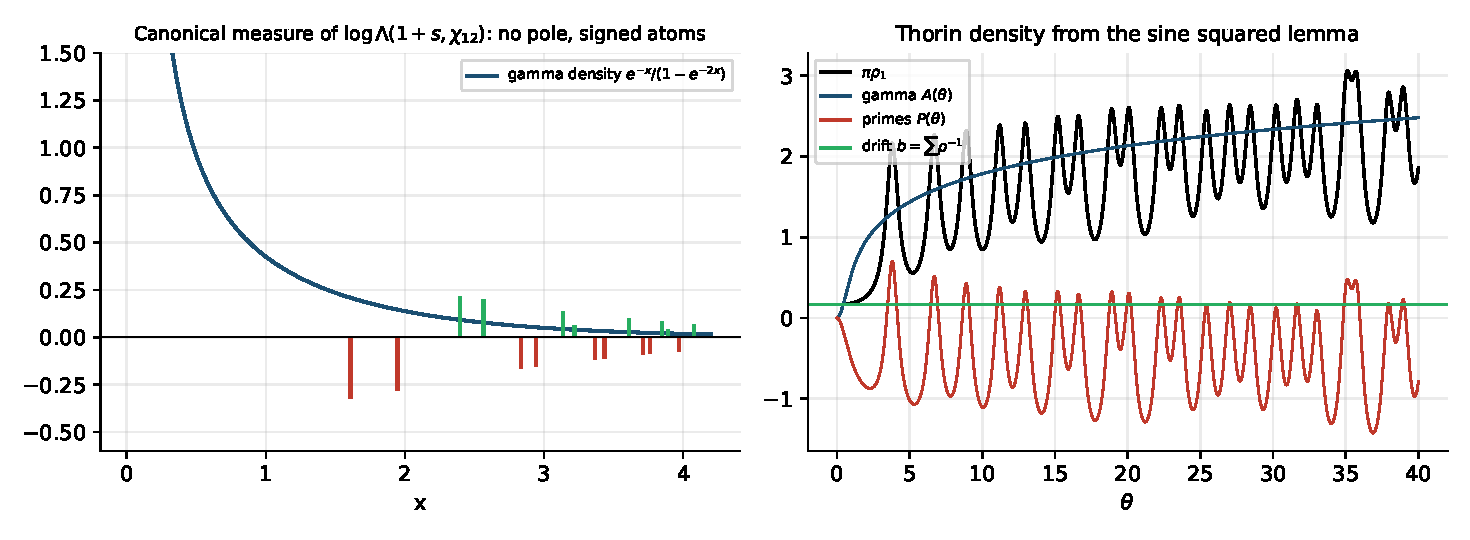
\includegraphics[width=\textwidth]{fig/bp1eta_levy.pdf}
\caption{Left: the canonical measure $x\Pi(dx)$ of $\log\xi(1+s,\chi_{12})$, written with $\Lambda(1+s,\chi_{12})$ in the plot: the positive gamma density $e^{-x}/(1-e^{-2x})$ and the prime atoms $\Lambda_{\chi_{12}}(n)/n$ at $\log n$, of both signs, the positive ones drawn upward and the negative ones downward; there is no pole. Right: $v_1(\theta)$ on $[0,40]$, written $\pi\rho_1$ in the plot, as the sum of the drift $b_1$, written $b$, the gamma piece $A(\theta)$ and the prime piece $Q(\theta)$, written $P(\theta)$ in the plot. Drawn by \texttt{figs.py} of \texttt{basepoint\_one/eta}.}
\label{bp:eta:fig:levy}
\end{figure}

\label{bp:eta:sec:below}Below the basepoint one, at $\alpha=1-\varepsilon$, the converted Thorin density is $\pi^{-1}$ times
\[
b_\alpha+A_\alpha(\theta)+\lim_{X\to\infty}\sum_{n\le X}\frac{\Lambda_{\chi_{12}}(n)}{n^\alpha}\,2\sin^2\Big(\frac{\theta\log n}2\Big),
\]
with $A_\alpha(\theta)=\frac12[\re\psi(\frac{\alpha+i\theta}2)-\psi(\frac\alpha2)]$. Exactly as for $\zeta$ in Proposition~\ref{bp:prop:below}, the limit exists and gives the positive Thorin density $v_\alpha/\pi$ when $L(s,\chi_{12})$ has no zeros with $\re s>\alpha'$ for some $\alpha'<\alpha$, and conversely its existence for $\re s>0$ in the L\'evy form forces the absence of zeros with $\re s>\alpha$. So the extension below one is, up to the boundary case, a zero free half plane for $L(s,\chi_{12})$, and at the centre it is GRH for $\chi_{12}$. The error at cutoff $X$ is given by the same explicit formula,
\[
\sum_\rho\Big[-\frac{X^{\rho-\alpha}}{\rho-\alpha}+\frac{X^{\rho-\alpha+i\theta}}{2(\rho-\alpha+i\theta)}+\frac{X^{\rho-\alpha-i\theta}}{2(\rho-\alpha-i\theta)}\Big]+O(X^{-\alpha}\log X),
\]
because $\psi(y,\chi_{12})=-\sum_\rho y^\rho/\rho+O(\log y)$ has no main term \cite[Chapter~19]{Davenport}.

The absence of a main term changes the numerics. For $\zeta$ the prime piece and the pole piece each grow like $X^{1-\alpha}/(1-\alpha)$ and must cancel; for $L(s,\chi_{12})$ the prime piece stays bounded. At $\alpha=0.6$, $\theta=\gamma_1$ and $X=10^7$ the prime piece is $6.07$, where for $\zeta$ the two pieces are about $1537$ each. Table~\ref{bp:eta:tab:below}, computed by \texttt{arith.py}, shows the errors, which decay like $X^{1/2-\alpha}$, and what remains after subtracting the explicit formula over the $297$ computed zeros. The correction removes most of the error at $\theta=\gamma_1$, by factors between $17$ and $2800$; at $\theta=10$, between zeros, it helps less, because $297$ zeros are fewer than the $1700$ used for $\zeta$ and the missing zeros above height $340$ dominate what remains. At the centre and the first ordinate the sum grows like $\log X$, taking the values $6.62$, $11.69$ and $16.77$ at $X=10^3$, $10^5$ and $10^7$: the atom $\delta_{\gamma_1}$ forming (Figure~\ref{bp:eta:fig:below}).

\begin{table}[htbp]
\centering\small
\begin{tabular}{cccccc}
\toprule
$\alpha$ & $\theta$ & $X$ & prime piece & error & error after zero correction\\
\midrule
1 & $\gamma_1$ & $10^5$ & 0.6964 & $-5.55\times10^{-3}$ & $4.2\times10^{-6}$\\
1 & $\gamma_1$ & $10^7$ & 0.7016 & $-4.15\times10^{-4}$ & $2.5\times10^{-5}$\\
0.75 & $\gamma_1$ & $10^5$ & 2.0933 & $-2.13\times10^{-1}$ & $1.4\times10^{-4}$\\
0.75 & $\gamma_1$ & $10^7$ & 2.2471 & $-5.92\times10^{-2}$ & $1.4\times10^{-3}$\\
0.6 & $\gamma_1$ & $10^5$ & 4.8292 & $-3.10$ & $1.1\times10^{-3}$\\
0.6 & $\gamma_1$ & $10^7$ & 6.0670 & $-1.86$ & $1.6\times10^{-2}$\\
0.6 & 10 & $10^7$ & $-2.4525$ & $-5.68\times10^{-2}$ & $2.6\times10^{-2}$\\
\bottomrule
\end{tabular}
\caption{The sine squared formula below the basepoint one for $L(s,\chi_{12})$, with primes up to $X$: the prime piece, the error against $v_\alpha(\theta)$, and the error left after subtracting the explicit formula over the $297$ computed zeros; $\gamma_1=3.8046276$.}
\label{bp:eta:tab:below}
\end{table}

\begin{figure}[htbp]
\centering
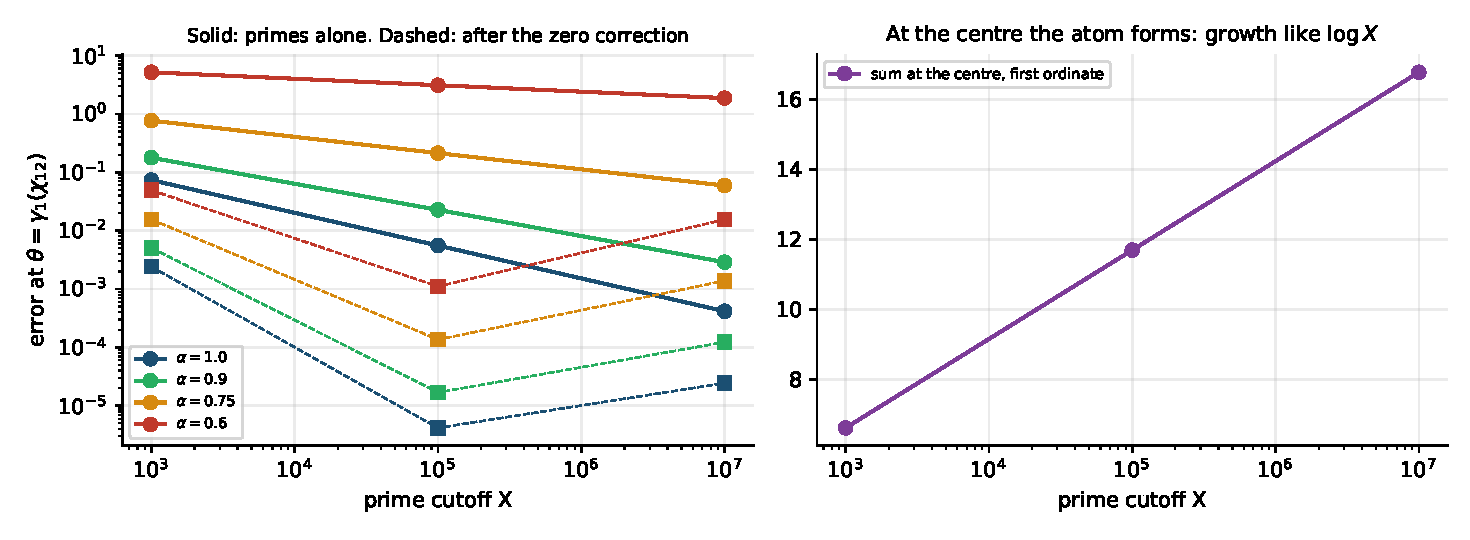
\includegraphics[width=\textwidth]{fig/bp1eta_below.pdf}
\caption{Left: absolute error at $\theta=\gamma_1=3.8046$ for $L(s,\chi_{12})$ against the prime cutoff $X$, for $\alpha=1$, $0.9$, $0.75$ and $0.6$, from primes alone (solid) and after the zero correction over $297$ zeros (dashed). Right: at the centre and the first ordinate the sum grows like $\log X$, the atom of the GRH measure forming. Drawn by \texttt{figs.py} of \texttt{basepoint\_one/eta}.}
\label{bp:eta:fig:below}
\end{figure}

\subsection{The hitting time and its boundary}\label{bp:eta:sec:hit}

The identity $(\frac12+\sqrt u)^2=\frac14+u+\sqrt u$ gives, as for $\zeta$,
\[
\varphi_1(u)=\frac{\varphi_{1/2}(\frac14+u+\sqrt u)}{\varphi_{1/2}(\frac14)},\qquad \varphi_{1/2}(u)=\frac{\xi(\frac12,\chi_{12})}{\xi(\frac12+\sqrt u,\chi_{12})} .
\]
Whenever the centre clock $\varphi_{1/2}$ is the Laplace transform of a probability law, and in particular under GRH for $\chi_{12}$, this reads $T_1\stackrel d=\widetilde T+H_{\widetilde T/\sqrt2}$, where $\widetilde T$ is the centre clock tilted by $e^{-T/4}$ and $H_a$ is the first passage time of Brownian motion to the level $a$, as in Theorem~\ref{bp:thm:sub}. Under GRH, $\widetilde T=\sum_ke_k/(\gamma_k^2+\frac14)$ with independent standard exponentials $e_k$; if the zeros are also simple, $\widetilde T$ is Kent's hitting time for a Krein string with spectrum $\{|\rho|^2\}$ \cite{Kent80}, and $T_1$ is the time for that string diffusion, run on the local time clock of a sticky Brownian motion, to reach its level, as in Corollary~\ref{bp:cor:kent}. As for $\zeta$, $T_1$ itself is not a hitting time of the kind in Kent's theorem, because its Thorin measure is absolutely continuous (Proposition~\ref{bp:eta:prop:thorin}).

We simulated $3\times10^5$ draws of $T_1$ with \texttt{hit.py}, taking $\widetilde T$ from this series under GRH: the terms of all $297$ computed zeros, and for the zeros above them a gamma variable matched to the tail sums of $p_1$ and $p_2$. The sample mean of $\widetilde T$ is $0.165108$ against $b_1=0.165083$, and the empirical Laplace transform agrees with $\varphi_1(u)=\xi(1,\chi_{12})/\xi(1+\sqrt u,\chi_{12})$ within $1.1$ standard errors at $u=0.1$, $0.5$, $1$, $5$ and $20$ (for instance $0.725800\pm0.000440$ against $0.726077$ at $u=1$, and $0.042364\pm0.000101$ against $0.042340$ at $u=20$).

We computed the Brownian boundary $b(t)$ whose crossing time has the law of $T_1$ from the Volterra equation \eqref{eq:ch19:volterra}, with the distribution function from Talbot inversion for $t<0.12$ and, under GRH as above, from the subordination representation beyond, and the complementary form of the equation once the survival probability falls below one half; \texttt{hit.py} solves it and \texttt{hit2.py} adds the tangent boundary and the checks. The time scale is about seven times that of $\zeta$, the ratio of the means of the two centre clocks. In the small time zone the boundary starts at the reflection level $1.008$ at $t=0.036$ and falls to $0.611$ at $t=0.08$; through the bulk it falls to $0.400$ at $t=0.12$ and $0.127$ at $t=0.2$, where the survival probability is one half; the tangent approximation agrees to $10^{-3}$ at $t=0.08$ and $5\times10^{-3}$ at $t=0.12$, then drifts, to $0.102$ at $t=0.2$. In the right tail the exact boundary flattens at $-0.2747$ ($-0.26030$ at $t=1$, $-0.27461$ at $t=100$, $-0.27471$ at $t=1000$), the Brownian form of the stable one half tail. The tangent approximation overshoots, to $-0.370$ at $t=0.4$ against the exact $-0.166$, and has no solution beyond $t=1.83$, for the reason explained in Section~\ref{bp:sec:rs1}: it cannot represent survivors that have wandered below the boundary.

Wald's identity fails in the same way as for $\zeta$, with the same proviso. The boundary is continuous and, as computed, bounded up to $t=1000$; if it is bounded on $[1,\infty)$, which here too is observed, not proved, Lemma~\ref{bp:lem:wald} and the stable tail give $\E\,b(T_1)=b_1/\sqrt2=\sum_\rho\rho^{-1}/\sqrt2=0.116732$; integrating the computed boundary against the law of $T_1$ gives $0.116749$. We simulated $1.5\times10^5$ Brownian paths against the exact boundary on $[0,5]$. Their survival function is within Kolmogorov distance $0.0014$ of the exact one (Figure~\ref{bp:eta:fig:hit}), and the simulated depth of the survivors below the boundary, $\E[(b(t)-B_t)\mathbf 1\{H_b>t\}]$, which tends to $\E\,b(T_1)$ by optional stopping, is $0.119$, $0.118$ and $0.118$ at $t=1$, $2$ and $5$.

\begin{figure}[htbp]
\centering
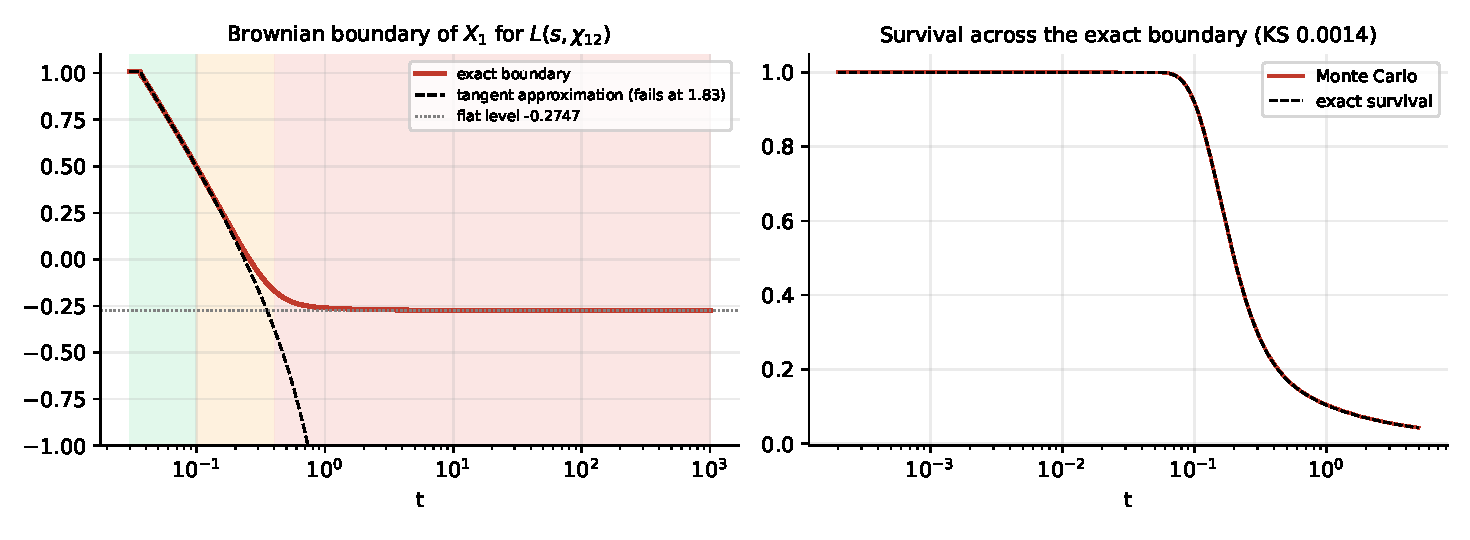
\includegraphics[width=\textwidth]{fig/bp1eta_hit.pdf}
\caption{Left: the exact Brownian boundary of $T_1$ for $L(s,\chi_{12})$, written $X_1$ in the plot, over the three zones of Section~\ref{sec:ch19:zones} (shaded), the tangent approximation, which fails at $t=1.83$, and the flat level $-0.2747$. Right: survival of $1.5\times10^5$ simulated Brownian paths across the exact boundary against the exact survival function; the Kolmogorov distance is $0.0014$. Drawn by \texttt{figs.py} of \texttt{basepoint\_one/eta}.}
\label{bp:eta:fig:hit}
\end{figure}

\subsection{The two examples compared}\label{bp:sec:compare}

Table~\ref{bp:eta:tab:cmp} sets the two basepoint one examples side by side. Structurally the eta case is the cleaner of the two: its kernel is a positive product, it has no pole, its L\'evy form converges at the basepoint one without compensation, and below the basepoint one its prime sums stay bounded, so the computation is far better conditioned. Nothing essential becomes easier, however. The negativity that $\zeta$ concentrates in the pole piece is carried here by the signs of $\chi_{12}(p)$; the extension of the L\'evy form below the line $\re s=1$ is equivalent to a zero free half plane for $L(s,\chi_{12})$; and, under GRH for $\chi_{12}$, the probabilistic picture is the same, with every constant scaled by the denser zeros: a stable one half subordination of the centre clock and, as computed, a boundary that flattens and, if it stays bounded, a Wald defect equal to $\sum_\rho\rho^{-1}/\sqrt2$.

\begin{table}[htbp]
\centering\small
\begin{tabular}{p{0.42\textwidth}p{0.26\textwidth}p{0.22\textwidth}}
\toprule
 & $\zeta$ & $L(s,\chi_{12})$\\
\midrule
kernel & theta series & $\eta(ix)$, a positive\newline product\\
pole & at $s=1$ & none\\
first zero & 14.134725 & 3.804628\\
drift $b_1=\sum_\rho\rho^{-1}$ & 0.0230957 & 0.1650833\\
tail constant $b_1/\sqrt\pi$ & 0.01303 & 0.09314\\
mean of the centre clock $\sum_ka_k^{-1}$ & 0.0231050 & 0.1664618\\
L\'evy measure, continuous part & gamma minus pole,\newline negative beyond $0.281$ & gamma only, positive\\
L\'evy measure, prime atoms & all positive & signs of $\chi_{12}(n)$\\
compensation at $\alpha=1$ & primes against $dx/x$\newline (prime number theorem) & none needed\\
prime piece at $\alpha=0.6$, $X=10^7$, $\theta=\gamma_1$ & about 1537,\newline cancelled by the pole & 6.07\\
flat level of the exact boundary & $-0.19277$ & $-0.27471$\\
$\E\,b(T_1)=b_1/\sqrt2$ & 0.016331 & 0.116732\\
tangent approximation fails at & $t=0.091$ & $t=1.83$\\
\bottomrule
\end{tabular}
\caption{The two basepoint one examples side by side: the reciprocal Xi function of Chapter~\ref{chap:basepoint} and the reciprocal completed $L$ function of $\chi_{12}$ of this section.}
\label{bp:eta:tab:cmp}
\end{table}

The comparison also closes the study of the basepoint one begun in Chapter~\ref{chap:basepoint}, and it confirms the two conclusions that fix the shape of the path to RH. First, at the basepoint one the constructions for the reciprocal Xi function are, with two exceptions, unconditional and explicit: the Thorin measure is the Poisson smoothing of the zeros, the L\'evy form comes from the primes, the gamma factor and the pole, the sine squared lemma converts one into the other with the drift $\sum_\rho\rho^{-1}$ becoming a stable one half factor, and the shifted clock is a subordinated hitting time whose Brownian boundary, as computed, becomes flat. The exceptions are the Krein string representation of Corollary~\ref{bp:cor:kent}, which assumes RH and simple zeros, and the Wald defect $\sum_\rho\rho^{-1}/\sqrt2$: Lemma~\ref{bp:lem:wald} gives it for a boundary bounded at infinity, and the boundedness of the computed boundary is observed, not proved. Second, below the basepoint one each positive statement for $\zeta$ holds, up to the boundary case, exactly when no zero lies to the right of the line $\re s=\alpha$: the convergence of the compensated L\'evy form, the GGC property of $T_\alpha$, the extended GGC property of the normal scale mixture, and the completeness in $L^1$ of the translates of the tilted P\'olya kernels on every line to the right of $\alpha$ (Propositions~\ref{bp:prop:below} and \ref{wr:prop:wiener}, Theorems~\ref{bp:thm:alpha} and \ref{sm:thm:strip}). The eta example shows that the pole changes how the prime sums converge, not where they stop.

The step that none of these constructions supplies is positivity of the Thorin measure at every height at a single basepoint $\alpha<1$, that is, the GGC property of $T_\alpha$, which by Theorem~\ref{thm:poisson} is a new zero free half plane, and then all the way to the centre. The variable $T_\alpha=\sigma^{(\alpha)}_{\widetilde T_\alpha}$ of Theorem~\ref{bp:thm:alpha} exists for every $\alpha>\frac12$ with no hypothesis, so only its GGC property is conditional; as $\alpha\downarrow\frac12$ the subordinator tends to pure drift, and the positivity must be supplied by the zeros themselves. Reaching any single $\alpha<1$ is step~7 of the path in Table~\ref{tab:ch25:path}, which the results of Sato and Bondesson do not reach either (Section~\ref{sb:sec:cannot}); for the methods of this book the basepoint one is where the path leaves the region of theorems. The half plane $\re s>\frac78$ announced in October 2026 for $\zeta$ and every Dirichlet $L$ function, $L(s,\chi_{12})$ included, would move that boundary to $\frac78$ by arithmetic from outside the book (Section~\ref{sec:ch25:open}).

\section{Almost generalised gamma convolutions}\label{ch:almost}

Below the basepoint one, as Section~\ref{bp:sec:compare} concluded, every positive object built so far from the shifted clock $T_\alpha$, whose Laplace transform is $\varphi_\alpha(u)=\xi(\alpha)/\xi(\alpha+\sqrt u)$, is equivalent, up to the boundary case, to the absence of zeros in the half plane $\re s>\alpha$. These equivalences are restatements rather than reductions. Since no zero free half plane was known before 2026, and none is known to the left of the line $\re s=\frac78$ (Section~\ref{sec:ch25:open}), the question that remains is quantitative: how negative can the Thorin density be below the basepoint one? Zero density estimates answer it with no hypothesis: with those of Ingham, of Guth and Maynard and of Huxley, every $T_\alpha$ with $\alpha>\frac12$ is a GGC up to a defect carried by the zeros to the right of $\alpha$, whose Cauchy kernels carry a vanishing fraction of the mass of the others, with a power saving; we call this property almost GGC.

With $\xi$ again in place of $\xi(\cdot,\chi_{12})$, we keep the notation of Sections~\ref{ch:basepoint} and \ref{ch:sato}: $v_\alpha(\theta)=\re(\xi'/\xi)(\alpha+i\theta)$, and the Thorin density at the basepoint $\alpha$ in the chart $\theta=\sqrt z$ is $v_\alpha/\pi$, the density $\rho_{\alpha-1/2}$ of \eqref{eq:rho} at the resolution $\alpha-\frac12$; in this section the basepoint, not the resolution, is the index. $P_w(x)=w/(\pi(w^2+x^2))$ is the Poisson kernel of Section~\ref{ch:clock}, $P_{-w}=-P_w$, and $P_0$ is the unit point mass, as in Proposition~\ref{prop:signature}. A zero is $\rho=\beta+i\gamma$; $N(T)$ counts the zeros with $0<\gamma\le T$, and $N(\sigma,T)$ those among them with $\beta\ge\sigma$, so that $N(\sigma,T)\ge\nu(\sigma,T)$ in the notation of Proposition~\ref{prop:zerodensity}.

\subsection{Mass bookkeeping and the almost GGC theorem}\label{ag:sec:almost}

The Poisson form of Proposition~\ref{prop:struct} splits according to the side of the line $\re s=\alpha$ on which each zero lies, $v_\alpha=v_\alpha^+-v_\alpha^-$, with
\begin{equation}\label{ag:eq:split}
\begin{aligned}
\frac{v_\alpha^+(\theta)}\pi&=\sum_{\beta\le\alpha,\ \gamma>0}\big[P_{\alpha-\beta}(\theta-\gamma)+P_{\alpha-\beta}(\theta+\gamma)\big],\\
\frac{v_\alpha^-(\theta)}\pi&=\sum_{\beta>\alpha,\ \gamma>0}\big[P_{\beta-\alpha}(\theta-\gamma)+P_{\beta-\alpha}(\theta+\gamma)\big].
\end{aligned}
\end{equation}
Both parts are positive, and a zero on the line $\re s=\alpha$, if there is one, contributes a unit atom at its ordinate to the positive part. Each pair of kernels has mass one on $(0,\infty)$. A zero with $\beta>\alpha$ has the partner $1-\bar\rho=1-\beta+i\gamma$, whose real part $1-\beta<\frac12<\alpha$ puts it in the positive part. Write $m_\alpha^\pm(T)=\pi^{-1}\int_0^Tv_\alpha^\pm(\theta)\,d\theta$ for the positive and negative masses on $[0,T]$.

\begin{lemma}[Mass bookkeeping]\label{ag:lem:mass}
Let $\alpha>\frac12$, and suppose that $N(\alpha,t)\le t^{e+o(1)}$ as $t\to\infty$ for some $e<1$. Then
\[
m_\alpha^-(T)\le N(\alpha,2T)+O\big(T^{e-1+o(1)}\big),\qquad m_\alpha^+(T)=\frac T{2\pi}\log\frac T{2\pi}+O(T).
\]
\end{lemma}

\begin{proof}
A zero with $\beta>\alpha$ and $\gamma\le2T$ contributes at most its total mass one. For a zero with $\gamma>2T$ put $w=\beta-\alpha$, so that $0<w<\frac12$. Since $\int_0^TP_w(\theta+\gamma)\,d\theta=\int_{-T}^0P_w(\theta-\gamma)\,d\theta$, its pair of kernels has mass on $[0,T]$ at most
\[
\int_{-\infty}^TP_w(\theta-\gamma)\,d\theta\le\frac{w}{\pi(\gamma-T)}\le\frac1{\pi\gamma},
\]
and $\sum_{\beta>\alpha,\ \gamma>2T}\gamma^{-1}=\int_{2T}^\infty t^{-1}dN(\alpha,t)\le\int_{2T}^\infty N(\alpha,t)t^{-2}dt\ll T^{e-1+o(1)}$. The positive part contains the kernels of all zeros with $\beta\le\alpha$, among them every zero on the critical line and every partner $1-\bar\rho$. Its mass on $[0,T]$ is therefore $N(T)$ up to the $N(\alpha,T)=O(T^{e+o(1)})$ zeros to the right of $\alpha$, whose kernels it lacks, and up to the tails of the kernels of the zeros near height $T$, which change it by $O(\log^2T)$. Since $N(T)=\frac T{2\pi}\log\frac T{2\pi}-\frac T{2\pi}+O(\log T)$, the second claim follows.
\end{proof}

\begin{theorem}[Almost GGC]\label{ag:thm:almost}
For every $\frac12<\alpha<1$, with no hypothesis,
\[
\frac{m_\alpha^-(T)}{m_\alpha^+(T)}\le T^{e(\alpha)-1+o(1)},\qquad e(\alpha)=\begin{cases}\dfrac{3(1-\alpha)}{2-\alpha},&\frac12<\alpha<\frac7{10},\\[2ex]\dfrac{15(1-\alpha)}{3+5\alpha},&\frac7{10}\le\alpha<1,\end{cases}
\]
and $e(\alpha)<1$ throughout, so the negative part $v_\alpha^-/\pi$ of \eqref{ag:eq:split}, the Cauchy kernels of the zeros to the right of $\alpha$, carries on $[0,T]$ a vanishing fraction of the mass of the positive part, with a power saving. For $\alpha\ge1$ no zero lies to the right of $\alpha$, and $m_\alpha^-=0$. Under the density hypothesis $e(\alpha)=2(1-\alpha)$. RH holds if and only if $v_\alpha^-$ vanishes identically for every $\alpha>\frac12$.
\end{theorem}

\begin{proof}
Combine Lemma~\ref{ag:lem:mass} with three zero density estimates: Ingham's $N(\sigma,T)\ll T^{3(1-\sigma)/(2-\sigma)}\log^5T$ \cite{Ingham40}; Guth and Maynard's $N(\sigma,T)\le T^{15(1-\sigma)/(3+5\sigma)+o(1)}$ for $\frac7{10}\le\sigma\le\frac45$ \cite[Theorem 1.2]{GM26}; and Huxley's $N(\sigma,T)\le T^{3(1-\sigma)/(3\sigma-1)+o(1)}$ for $\sigma\ge\frac34$ \cite{Huxley72}, whose exponent is at most $15(1-\sigma)/(3+5\sigma)$ when $\sigma\ge\frac45$. Since $3(1-\alpha)<2-\alpha$ exactly when $\alpha>\frac12$, and $15(1-\alpha)<3+5\alpha$ exactly when $\alpha>\frac35$, the exponent is below one for every $\frac12<\alpha<1$. Finally, $v_\alpha^-$ vanishes identically exactly when no zero has $\beta>\alpha$, which is the GGC criterion of Theorem~\ref{thm:poisson}.
\end{proof}

Even the classical estimate of Bohr and Landau \cite{BL14}, $N(\sigma,T)=O(T)$ for fixed $\sigma>\frac12$, gives a vanishing fraction $O(1/\log T)$; the zero density estimates improve this to a power of $T$. First, the theorem bounds the decomposition mass $m_\alpha^-(T)$, which overcounts the negative part $\int_0^T\max(-v_\alpha/\pi,0)\,d\theta$ of the density itself, because the positive kernels of nearby zeros cancel much of each negative kernel. The partner of a zero already cancels part of it: with $\varepsilon=\alpha-\frac12$ and $\delta=\beta-\frac12$, twice the mass in Proposition~\ref{prop:signature}(iii) gives the negative part of $P_{\alpha+\beta-1}-P_{\beta-\alpha}=P_{\varepsilon+\delta}+P_{\varepsilon-\delta}$ the mass $\frac4\pi\arctan\sqrt{(\delta+\varepsilon)/(\delta-\varepsilon)}-1=\frac2\pi\arcsin\frac\varepsilon\delta$, less than the mass one that the decomposition counts, and Section~\ref{ag:sec:num} shows the effect of the other zeros. Second, on the verified range the negative mass is essentially zero. All zeros with $0<\gamma\le T_0$ lie on the critical line \cite{PT21}, so for $T\le T_0/2$ the only negative contributions come from zeros above $T_0$, and by the proof of Lemma~\ref{ag:lem:mass} their total mass on $[0,T]$ is $O(T_0^{e(\alpha)-1+o(1)})$.

The left panel of Figure~\ref{ag:fig:almost} draws the exponents. The saving $1-e(\alpha)$ is small near the centre, where Ingham's exponent gives $(2\alpha-1)/(2-\alpha)$. Sharper exponents are known near $\alpha=1$: the density hypothesis itself holds for $\alpha>\frac{25}{32}$ \cite[p.~133]{Bourgain00}, and Huxley's exponent \cite{Huxley72} is $0.176$ at $\alpha=0.9$; those of the theorem suffice for what follows.

\subsection{The canonical factorisation and explicit unconditional bounds}\label{ag:sec:factor}



\begin{proposition}[Canonical factorisation]\label{ag:prop:factor}
For every $\alpha>\frac12$ and $u\ge0$, $\varphi_\alpha(u)=\varphi_\alpha^+(u)\,D_\alpha(u)$, where
\begin{gather*}
\varphi_\alpha^+(u)=\exp\Big\{-\int_0^\infty\log\Big(1+\frac u{\theta^2}\Big)\frac{v_\alpha^+(\theta)}\pi\,d\theta\Big\},\\
D_\alpha(u)=\prod_{\beta>\alpha,\ \gamma>0}\frac{(\beta-\alpha)^2+\gamma^2}{(\sqrt u-\beta+\alpha)^2+\gamma^2};
\end{gather*}
here $\varphi_\alpha^+$ is the Laplace transform of a GGC $T_\alpha^+$ with Thorin density $v_\alpha^+/\pi$ in the chart $\theta=\sqrt z$, and the product defining the defect $D_\alpha$ runs over the zeros to the right of the line $\re s=\alpha$ and converges absolutely. The defect is identically one if and only if $\zeta$ has no zeros with $\re s>\alpha$, and then $T_\alpha\stackrel d=T_\alpha^+$. Otherwise $D_\alpha(u)\to0$ as $u\to\infty$, and $T_\alpha^+$ is not the sum of $T_\alpha$ and an independent nonnegative variable.
\end{proposition}

\begin{proof}
Grouping the Hadamard product of $\xi$ in conjugate pairs, as in the proof of Proposition~\ref{prop:struct}, gives for $u\ge0$
\[
\varphi_\alpha(u)=\prod_{\gamma>0}\frac{(\alpha-\beta)^2+\gamma^2}{(\alpha-\beta+\sqrt u)^2+\gamma^2},
\]
over the zeros with $\gamma>0$, counted with multiplicity; each factor is $1+O((u+\sqrt u)\gamma^{-2})$ and $\sum\gamma^{-2}<\infty$, so the product converges absolutely. For $\beta<\alpha$, with $w=\alpha-\beta>0$, the factor is $(w^2+\gamma^2)/((w+\sqrt u)^2+\gamma^2)=\exp\{-\int_0^\infty\log(1+u/\theta^2)[P_w(\theta-\gamma)+P_w(\theta+\gamma)]\,d\theta\}$, the Laplace transform of a GGC whose Thorin density is the pair of Cauchy kernels of width $w$ at $\pm\gamma$ (the computation after Theorem~\ref{sm:thm:thorin}); for $\beta=\alpha$ it is $\gamma^2/(\gamma^2+u)$, an exponential law, whose Thorin measure is the atom at $\gamma$. The partial products over the zeros with $\beta\le\alpha$ are therefore Laplace transforms of GGCs, they converge for every $u\ge0$ to a limit continuous at the origin, and by the closure theorem of Section~\ref{sec:weak:limits} the limit is the Laplace transform of a GGC, with Thorin density $v_\alpha^+/\pi$. The remaining factors form $D_\alpha$. If a zero lies to the right of $\alpha$, put $w=\beta-\alpha\in(0,\frac12)$; its factor tends to zero as $u\to\infty$, and every factor of $D_\alpha$ is at most one for $u\ge1$, because $(\sqrt u-w)^2\ge w^2$ when $\sqrt u\ge2w$. So $D_\alpha(u)\to0$. If $T_\alpha^+$ were $T_\alpha+S$ with $S\ge0$ independent of $T_\alpha$, then $\E e^{-uS}=\varphi_\alpha^+(u)/\varphi_\alpha(u)=1/D_\alpha(u)$ would be unbounded, which is impossible.
\end{proof}

The proposition also says what the signed density $v_\alpha/\pi$ is. When every zero lies to the left of the line $\re s=\alpha$ it is the Thorin density of $T_\alpha$ (Theorem~\ref{thm:poisson}); a zero on the line adds to the Thorin measure an atom at its ordinate, the term $P_0$ of \eqref{ag:eq:split}, which the function $v_\alpha$ does not show. When a zero lies to the right of the line, $T_\alpha$ is not a GGC and $v_\alpha/\pi$ is not a signed Thorin density for it in any sense: the negative kernel $-P_w$ of such a zero integrates to the factor $((w+\sqrt u)^2+\gamma^2)/(w^2+\gamma^2)$, while the zero contributes $(w^2+\gamma^2)/((\sqrt u-w)^2+\gamma^2)$ to $\varphi_\alpha$. The bookkeeping of Theorem~\ref{ag:thm:almost} applies to the other reformulations in Chapters~\ref{chap:basepoint} to \ref{chap:almost}. In the normal scale mixture of Theorem~\ref{sm:thm:strip} it bounds the negative part of the candidate EGGC density $v_\alpha/\pi$; in Wiener's theorem (Proposition~\ref{wr:prop:wiener}) it bounds the proportion of frequencies at which the Fourier transform of the tilted P\'olya kernel can vanish; and in Riesz's criterion (Section~\ref{wr:sec:riesz}) it bounds the number of Mellin poles to the right of $\alpha/2$.

The pole factors can be written down. Let $U_\alpha^\circ$ denote the signed measure on $\theta>0$ with density $v_\alpha/\pi$ and a unit atom at $\gamma$ for every zero $\beta+i\gamma$, $\gamma>0$, with $\beta=\alpha$ (the term $P_0$ of \eqref{ag:eq:split}), counted with multiplicity.

\begin{theorem}[Signed Thorin representation]\label{tx:thm:signed}
For every $\alpha\ge\frac12$ and $u\ge0$,
\[
\varphi_\alpha(u)=\exp\Big\{-\int_0^\infty\log\Big(1+\frac u{\theta^2}\Big)U_\alpha^\circ(d\theta)\Big\}\prod_{\beta>\alpha,\ \gamma>0}\Big|1-\frac u{(\rho-\alpha)^2}\Big|^{-2},
\]
the integral and the product converging absolutely. For a zero to the right of $\alpha$, with $p=(\rho-\alpha)^2=-c+id$, $c=\gamma^2-(\beta-\alpha)^2>0$ and $d=2\gamma(\beta-\alpha)>0$, the factor is
\[
\Big|1-\frac up\Big|^{-2}=\frac{|p|^2}{(u+c)^2+d^2}=|p|^2\int_0^\infty e^{-ut}\,\frac{e^{-ct}\sin dt}d\,dt,
\]
the Laplace transform of a damped sinusoid, which changes sign, so the factor is not completely monotone.
\end{theorem}

\begin{proof}
Write $f_w(u)=(w^2+\gamma^2)/((w+\sqrt u)^2+\gamma^2)$. By the Hadamard product, as in the proof of Proposition~\ref{ag:prop:factor}, $\varphi_\alpha(u)=\prod_{\gamma>0}f_{\alpha-\beta}(u)$ over all zeros with $\gamma>0$, absolutely convergent. For $w\ge0$ that proof gives $f_w(u)=\exp\{-\int_0^\infty\log(1+u/\theta^2)[P_w(\theta-\gamma)+P_w(\theta+\gamma)]\,d\theta\}$, with the atom at $\gamma$ for $w=0$. For $w=-\omega<0$ the kernels carry the sign $P_{-\omega}=-P_\omega$, so the same integral equals $f_\omega^{-1}$, and a direct computation gives $f_{-\omega}=f_\omega^{-1}\,|p|^2/|p-u|^2$ with $p=(\omega+i\gamma)^2$, since $|p-u|^2=((\sqrt u-\omega)^2+\gamma^2)((\sqrt u+\omega)^2+\gamma^2)$. Multiplying over the zeros gives the formula, once the integrals are summed under the integral sign: the integral of each pair of kernels against $\log(1+u/\theta^2)$ is $\pm\log f_{|w|}$, which is $O_\alpha((u+\sqrt u)\gamma^{-2})$, and $\sum\gamma^{-2}<\infty$. Finally $|p-u|^2=(u+c)^2+d^2$, and $c>0$ because $\beta-\alpha<\frac12<\gamma_1$.
\end{proof}

The theorem needs no hypothesis on the zeros: the atoms carry the zeros on the line $\re s=\alpha$, which is why the case $\alpha=\frac12$ is included. It is the identity behind Proposition~\ref{ag:prop:factor}, which combines the pole factors with the negative kernels they cancel into $D_\alpha$. At $\alpha=\frac12$ every term is explicit.

\begin{corollary}[The critical line]\label{tx:cor:half}
Unconditionally, $U_{1/2}^\circ=\sum_{\beta=1/2,\ \gamma>0}\delta_\gamma\ge0$ and
\[
\varphi_{1/2}(u)=\prod_{\beta=1/2,\ \gamma>0}\frac{\gamma^2}{\gamma^2+u}\ \prod_{\beta>1/2,\ \gamma>0}\Big|1-\frac u{(\rho-\frac12)^2}\Big|^{-2}.
\]
\end{corollary}

\begin{proof}
A zero $\rho$ with $\beta=\frac12+\delta$, $\delta>0$, and its partner $1-\bar\rho$ have the same ordinate, and their kernels $P_{-\delta}+P_\delta$ cancel, so $v_{1/2}=0$ away from the atoms (the term by term form in the proof of Proposition~\ref{prop:struct}, which holds at $\alpha=\frac12$ away from the ordinates). The atoms come from the zeros with $\beta=\frac12$, each with the factor $f_0=\gamma^2/(\gamma^2+u)$; apply Theorem~\ref{tx:thm:signed}.
\end{proof}

So on the critical line positivity of $U_{1/2}^\circ$ costs nothing, and RH is the statement that the product of damped sinusoids is empty. For $\frac12<\alpha<\sup_\rho\re\rho$ the negative kernels of Proposition~\ref{ag:prop:factor} are present, and whether they can be outweighed on the single line $\re s=\alpha$ is open, except near a zero, where they cannot (Remark~\ref{rem:ch2:oneline}).

\begin{theorem}[Explicit bounds from verification]\label{ag:thm:explicit}
Let $T_0=3\times10^{12}$, below which all zeros lie on the critical line \cite{PT21}, and let $\Sigma_0=\sum_{\gamma>T_0}\gamma^{-2}$, the sum over all zeros above $T_0$, counted with multiplicity. By the Riemann von Mangoldt formula with the explicit error term of Hasanalizade, Shen and Wong \cite{HSW22}, recalled in the proof of Proposition~\ref{bp:prop:v1min}, $\Sigma_0$ differs from $\frac{\log(T_0/2\pi)+1}{2\pi T_0}=1.4797\times10^{-12}$ by less than $2\times10^{-24}$, so $\Sigma_0<1.48\times10^{-12}$. Then for every $\alpha>\frac12$ and every $u\ge0$:
\begin{enumerate}
\item $|\log D_\alpha(u)|\le(u+\sqrt u)\,\Sigma_0$, so that
\[
e^{-1.5\times10^{-12}(u+\sqrt u)}\,\varphi_\alpha^+(u)\le\E e^{-uT_\alpha}\le e^{1.5\times10^{-12}(u+\sqrt u)}\,\varphi_\alpha^+(u);
\]
\item the negative part of the density satisfies $v_\alpha^-(\theta)/\pi\le2\Sigma_0/\pi<9.43\times10^{-13}$ for $0\le\theta\le T_0/2$;
\item consequently $v_\alpha(\theta)>0$ for all $0\le\theta\le T_0/2$ whenever $\alpha-\frac12>6\times10^{-10}$.
\end{enumerate}
\end{theorem}

\begin{proof}
Every zero to the right of $\alpha$ has $\gamma>T_0$ and $\beta>\frac12$. The zeros above $T_0$ off the critical line come in pairs $\beta+i\gamma$, $1-\beta+i\gamma$ of equal multiplicity, by $\xi(s)=\xi(1-s)$ and $\xi(\bar s)=\overline{\xi(s)}$, and at most one member of each pair lies to the right of $\alpha$, so $\sum_{\beta>\alpha,\ \gamma>0}\gamma^{-2}\le\Sigma_0/2$. (1) For a zero to the right of $\alpha$ put $w=\beta-\alpha\in(0,\frac12)$ and $x=(u-2w\sqrt u)/(w^2+\gamma^2)$, so that its factor in $D_\alpha$ is $1/(1+x)$. Since $u-2w\sqrt u\ge-w^2$, we have $x\ge-w^2/\gamma^2>-\frac12$, and $|x|\le(u+\sqrt u)/\gamma^2$; for $x\ge-\frac12$, $|\log(1+x)|\le2|x|$. Hence the logarithm of its factor is at most $2(u+\sqrt u)/\gamma^2$ in absolute value, and summing gives $|\log D_\alpha(u)|\le(u+\sqrt u)\Sigma_0$; the inequalities for $\E e^{-uT_\alpha}=\varphi_\alpha^+(u)D_\alpha(u)$ follow. (2) For $\theta\le T_0/2$ and $\gamma>T_0$, $P_w(\theta-\gamma)+P_w(\theta+\gamma)\le\frac{2w}{\pi(\gamma-\theta)^2}\le\frac4{\pi\gamma^2}$, and summing over the zeros to the right of $\alpha$ gives at most $\frac4\pi\cdot\frac{\Sigma_0}2$. (3) Write $a=\alpha-\frac12$. If $a\ge\frac12$, then $\alpha\ge1$, no zero lies to the right of $\alpha$, and $v_\alpha=v_\alpha^+>0$; so let $6\times10^{-10}<a<\frac12$. The zeros below $T_0$ lie on the line and contribute to $v_\alpha^+/\pi$ the kernels $P_a(\theta-\gamma)$, and all other kernels of $v_\alpha^+$ are positive, so $v_\alpha^+(\theta)/\pi\ge\frac a{\pi(a^2+\gamma_1^2)}$ at every $\theta$ within $\gamma_1$ of an ordinate below $T_0$. Every $\theta\in[0,T_0/2]$ is such a point. On $[0,\gamma_1]$ the ordinate $\gamma_1$ serves. On $[\gamma_1,2000]$ one of the first $1800$ ordinates serves: they are the certified zeros of the proof of Proposition~\ref{bp:prop:v1min}, they reach height $2304.3$, and consecutive ones differ by less than $6.8874<2\gamma_1$. For $2000\le\theta\le T_0/2$, the count of that proof, with $H=14$ in place of $15$, shows that the window $(\theta-14,\theta+14]$ holds at least $n(\theta)=\frac{14}\pi\log\frac{\theta-14}{2\pi}-E(\theta-14)-E(\theta+14)$ zeros; while $\theta+14\le X_0$, $n$ increases and $n(2000)>20$, and for $\theta+14>X_0$, $n(\theta)>\frac{14}\pi\log\frac{\theta-14}{2\pi}-0.6\log(\theta+14)>80$, so the window holds a zero, which lies within $14<\gamma_1$ of $\theta$ and, since $\theta+14<T_0$, on the line. The script \texttt{explicit\_bounds.py}, with output \texttt{explicit\_bounds.json}, recomputes the $1800$ zeros and checks these inequalities in ball arithmetic. Finally, since $a<\frac12$,
\[
\frac a{\pi(a^2+\gamma_1^2)}>\frac a{\pi(\frac14+\gamma_1^2)}>\frac{6\times10^{-10}}{\pi(\frac14+\gamma_1^2)}>9.5\times10^{-13},
\]
which is more than the bound $2\Sigma_0/\pi<9.43\times10^{-13}$ of (2) on $v_\alpha^-/\pi$, so $v_\alpha=v_\alpha^+-v_\alpha^->0$ on $[0,T_0/2]$.
\end{proof}

Theorem~\ref{ag:thm:explicit} restates the verification of RH to height $3\times10^{12}$ in Thorin form. Part (3) of Theorem~\ref{sm:thm:strip} is the same statement for the characteristic function of the normal scale mixture, with a remainder of relative size $\log T_0/T_0$, and the paragraph after its proof bounds the negative part of $v_\alpha/\pi$ for $\theta\le10^9$ in the same way as part (2).

Part (3) of Theorem~\ref{ag:thm:explicit} treats every zero above $T_0$ as if its kernel could be negative wherever the density is evaluated. As the first author's note on the Dirichlet beta function observes \cite{P26beta}, grouping each such zero with its reflection in the critical line does better, because the sum of the two kernels of an off line pair is negative only near its ordinate.

\begin{corollary}[Positivity on the verified window]\label{cor:dbeta:window}
Let $T_0=3\times10^{12}$ and $V_\xi=(\log\xi)''(\frac12)=0.04620998623$.
\begin{enumerate}
\item For every $\alpha>\frac12$, $v_\alpha(\theta)>0$ for $|\theta|\le T_0-\frac12$.
\item For every $\alpha\in(\frac12,7.35]$, $v_\alpha(\theta)>v_\alpha(0)$ for $0<|\theta|\le T_0-\frac{1+\sqrt2}2$, and $0<v_\alpha(0)\le(\alpha-\frac12)V_\xi$.
\end{enumerate}
\end{corollary}

\begin{proof}
(1) Put $\varepsilon=\alpha-\frac12$. By the Hadamard product, as in Proposition~\ref{prop:struct}, $v_\alpha(\theta)$ is the absolutely convergent sum over the zeros $\rho=\beta+i\gamma$, counted with multiplicity, of $(\alpha-\beta)/((\alpha-\beta)^2+(\theta-\gamma)^2)$. A zero on the critical line contributes $\pi P_\varepsilon(\theta-\gamma)>0$. The zeros off the line come in pairs $\frac12\pm\delta+i\gamma$ with $0<\delta<\frac12$ and equal multiplicities, and a pair contributes $\pi(P_{\varepsilon+\delta}+P_{\varepsilon-\delta})(\theta-\gamma)$, which is nonnegative if $\delta\le\varepsilon$ and, if $\delta>\varepsilon$, negative exactly where $|\theta-\gamma|<\sqrt{\delta^2-\varepsilon^2}$, by the proof of Proposition~\ref{prop:signature}(ii); and $\sqrt{\delta^2-\varepsilon^2}<\delta<\frac12$. Every zero off the line has $|\gamma|>T_0$ \cite{PT21}, so for $|\theta|\le T_0-\frac12$ every pair has $|\theta-\gamma|>\frac12$ and contributes a nonnegative term, while the zero $\frac12+i\gamma_1$ contributes a positive one.

(2) This is Theorem~\ref{thm:dbeta:minall}(i) and (ii) for $\xi$, with $\alpha_{\max}=7.35$ and $H_0=T_0$ (Table~\ref{tab:dbeta:minall}).
\end{proof}

\begin{remark}\label{rem:dbeta:window}
The corollary does not touch the defect of part (1) of Theorem~\ref{ag:thm:explicit}: a zero above $T_0$ to the right of the line $\re s=\alpha$ stops $T_\alpha$ from being a GGC whatever $v_\alpha$ does on the window (Proposition~\ref{ag:prop:factor}), and near its own ordinate it can make $v_\alpha$ negative (Section~\ref{ag:sec:cancel}).
\end{remark}

The proof of part (1) gives, with no hypothesis, $|\log D_\alpha(u)|\le2(u+\sqrt u)\sum_{\beta>\alpha,\ \gamma>0}\gamma^{-2}$. With the verification height and the trivial count the sum is at most $\Sigma_0/2$, with $\Sigma_0<1.48\times10^{-12}$. The zero density estimates of Section~\ref{ag:sec:almost} \cite{Ingham40,GM26,Huxley72} improve this to $\sum_{\beta>\alpha}\gamma^{-2}\le\int_{T_0}^\infty t^{-2}dN(\alpha,t)\ll T_0^{e(\alpha)-2+o(1)}$, smaller by a further power of $T_0$ since $e(\alpha)<1$.

\subsection{Where negativity can come from: a cancellation lemma}\label{ag:sec:cancel}

The counting bound treats every zero to the right of $\alpha$ as if its kernel were entirely negative. Pointwise, a negative kernel is cancelled wherever the rest of the density exceeds it, and the kernel of width $w$ has height at most $1/(\pi w)$.

\begin{lemma}[Cancellation]\label{ag:lem:cancel}
Let $\rho=\beta+i\gamma$ be a zero with $\beta>\alpha$, and let $m>0$ be a lower bound on an interval $I$ for the rest of the density, $v_\alpha/\pi+P_{\beta-\alpha}(\cdot-\gamma)$. If $\beta-\alpha\ge1/(\pi m)$, the kernel of $\rho$ cannot make $v_\alpha$ negative on $I$.
\end{lemma}

\begin{proof}
On $I$, $v_\alpha/\pi\ge m-\max_xP_{\beta-\alpha}(x)=m-1/(\pi(\beta-\alpha))\ge0$.
\end{proof}

The lemma has a heuristic consequence. At height $\gamma$ the density $v_\alpha/\pi$ averages $\frac1{2\pi}\log\frac\gamma{2\pi}$, the density of the ordinates, and when $\alpha-\frac12$ is large compared with the mean spacing $2\pi/\log\gamma$ it stays close to that average. Taking this average for $m$ in the lemma, a zero to the right of $\alpha$ can then produce negativity only if
\[
\beta-\alpha<\frac{2\pi}{\pi\log(\gamma/2\pi)}=\frac2{\log(\gamma/2\pi)} .
\]
Heuristically, then, positivity of the Thorin density at the basepoint $\alpha$ can be broken at height $\gamma$ only by zeros in the thin strip $\alpha<\beta<\alpha+2/\log(\gamma/2\pi)$. The local visibility condition of Section~\ref{sec:ch13:visibility}, which concerns small resolutions, has the same scale $1/\log\gamma$. The heuristic proves nothing, because a rigorous lower bound for the background near an arbitrary height would itself control $\zeta'/\zeta$ in the strip. It suggests combining zero density estimates for thin strips with lower bounds for $\re\xi'/\xi$ on average.

We tested the lemma at the heights $300$ and $10^5$ with \texttt{high.py}. The script computes the background $v_{0.6}/\pi$ from $\xi'/\xi$ on a window of width $8$ and adds the kernels of a single hypothetical pair of zeros at $\beta+i\gamma_0$ and $1-\beta+i\gamma_0$, with $\gamma_0$ the centre of the window (Figure~\ref{ag:fig:cancel}, middle and right). At height $300$ the background has mean $0.51$ and minimum $0.069$; at height $10^5$ it has mean $1.59$, close to the density of ordinates $\frac1{2\pi}\log\frac{10^5}{2\pi}=1.54$, and minimum $0.34$. Table~\ref{ag:tab:cancel} shows the result. At both heights zeros with $\beta-\alpha\le0.2$ produce negativity and zeros with $\beta-\alpha\ge0.3$ are absorbed. At height $10^5$ the heuristic threshold $2/\log(10^5/2\pi)=0.21$ is close to the observed one, while the rigorous guarantee of Lemma~\ref{ag:lem:cancel} with the window minimum, $1/(\pi m)=0.93$, is conservative. For a fixed width the negative dip is deeper at the greater height, because the kernel is the same while the local minimum of the background near the hypothetical zero differs.

\begin{table}[htbp]
\centering\small
\begin{tabular}{ccccc}
\toprule
 & \multicolumn{2}{c}{height 300} & \multicolumn{2}{c}{height $10^5$}\\
$\beta$ & min of $v_{0.6}/\pi$ & negative mass & min of $v_{0.6}/\pi$ & negative mass\\
\midrule
0.62 & $-13.54$ & 0.521 & $-13.97$ & 0.567\\
0.65 & $-4.16$ & 0.299 & $-4.59$ & 0.365\\
0.70 & $-1.24$ & 0.121 & $-1.62$ & 0.193\\
0.75 & $-0.41$ & 0.041 & $-0.72$ & 0.097\\
0.80 & $-0.10$ & 0.008 & $-0.32$ & 0.041\\
0.90 & $0.072$ & 0 & $0.023$ & 0\\
0.95 & $0.075$ & 0 & $0.100$ & 0\\
\bottomrule
\end{tabular}
\caption{A single hypothetical pair of zeros at real parts $\beta$ and $1-\beta$ inserted into the density $v_{0.6}/\pi$, computed from $\xi'/\xi$ on a window of width $8$ at the heights $300$ and $10^5$: the minimum of the density and the negative mass $\int\max(-v_{0.6}/\pi,0)$ on the window. Computed by \texttt{high.py}.}
\label{ag:tab:cancel}
\end{table}

\subsection{Hypothetical off line zeros in the computed density}\label{ag:sec:num}

No off line zero is known, so the negative part cannot be observed. To see the mechanism, \texttt{almost.py} inserts fifteen hypothetical quadruples of zeros $0.75\pm i\gamma_j$, $0.25\pm i\gamma_j$, at the heights $\gamma_j=20\,j^{5/3}$ below $2000$, into the Poisson form of Proposition~\ref{prop:struct} together with the first $1700$ ordinates, taken on the line; the zeros above height $2198$ are omitted. The count of the hypothetical zeros grows like $T^{0.6}$, as a zero density estimate with $e=0.6$ would allow. Table~\ref{ag:tab:syn} compares the negative mass $\int_0^T\max(-v_\alpha/\pi,0)\,d\theta$ of the resulting density with its positive mass and with the counting bound $N_{\rm off}(2T)$ of Lemma~\ref{ag:lem:mass}, the number of hypothetical zeros with ordinate at most $2T$.

\begin{table}[htbp]
\centering\small
\begin{tabular}{cccccc}
\toprule
$\alpha$ & $T$ & negative mass & positive mass & fraction & counting bound $N_{\rm off}(2T)$\\
\midrule
0.6 & 250 & 0.842 & 108.8 & $7.7\times10^{-3}$ & 6\\
0.6 & 1000 & 1.655 & 650.5 & $2.5\times10^{-3}$ & 15\\
0.6 & 2000 & 2.278 & 1519.2 & $1.5\times10^{-3}$ & 15\\
0.7 & 250 & 2.130 & 110.1 & $1.9\times10^{-2}$ & 6\\
0.7 & 1000 & 4.815 & 653.6 & $7.4\times10^{-3}$ & 15\\
0.7 & 2000 & 6.938 & 1523.8 & $4.6\times10^{-3}$ & 15\\
0.8 & any & 0 & & 0 & 0\\
\bottomrule
\end{tabular}
\caption{Negative and positive mass of the density $v_\alpha/\pi$ on $[0,T]$ with fifteen hypothetical quadruples of zeros at real part $0.75$. Computed by \texttt{almost.py}.}
\label{ag:tab:syn}
\end{table}

Three features are visible. The negative mass is well below the counting bound, because each negative kernel is partly cancelled by its partner and by the positive kernels of the neighbouring zeros on the line: at $\alpha=0.6$ the negative kernel has width $0.15$ and height $1/(0.15\pi)=2.1$, and most of it is cancelled, while at $\alpha=0.7$ the width is $0.05$ and the kernel, of height $6.4$, appears as a sharp negative spike that takes the density to $-5.39$ at the height $292.40$ (Figure~\ref{ag:fig:almost}; the minimum is computed by \texttt{almost\_dip.py}). The fraction decreases with $T$ at the rate the counting predicts. And at $\alpha=0.8$, to the right of the hypothetical zeros, the density is positive everywhere, as Theorem~\ref{thm:poisson} requires: a zero with real part $\beta$ contributes a positive kernel at every basepoint $\alpha>\beta$.

A zero is most visible from basepoints just to its left. The left panel of Figure~\ref{ag:fig:cancel}, computed by \texttt{more2.py}, shows the negative mass on $[0,2000]$ as a function of $\alpha$ for the same fifteen heights and three real parts $\beta=0.6$, $0.75$ and $0.9$. As $\alpha$ increases towards $\beta$ the negative kernels narrow, cancellation fails, and the negative mass climbs towards the number of hypothetical zeros, reaching $7.55$ at $\alpha=0.85$ for $\beta=0.9$. At $\alpha=\beta$ the zeros lie on the line of evaluation and the negative mass drops to zero. This is the Thorin counterpart of the fact that the translates of the tilted P\'olya kernel fail to be complete exactly on the line through the zero (Proposition~\ref{wr:prop:wiener}).

\begin{figure}[htbp]
\centering
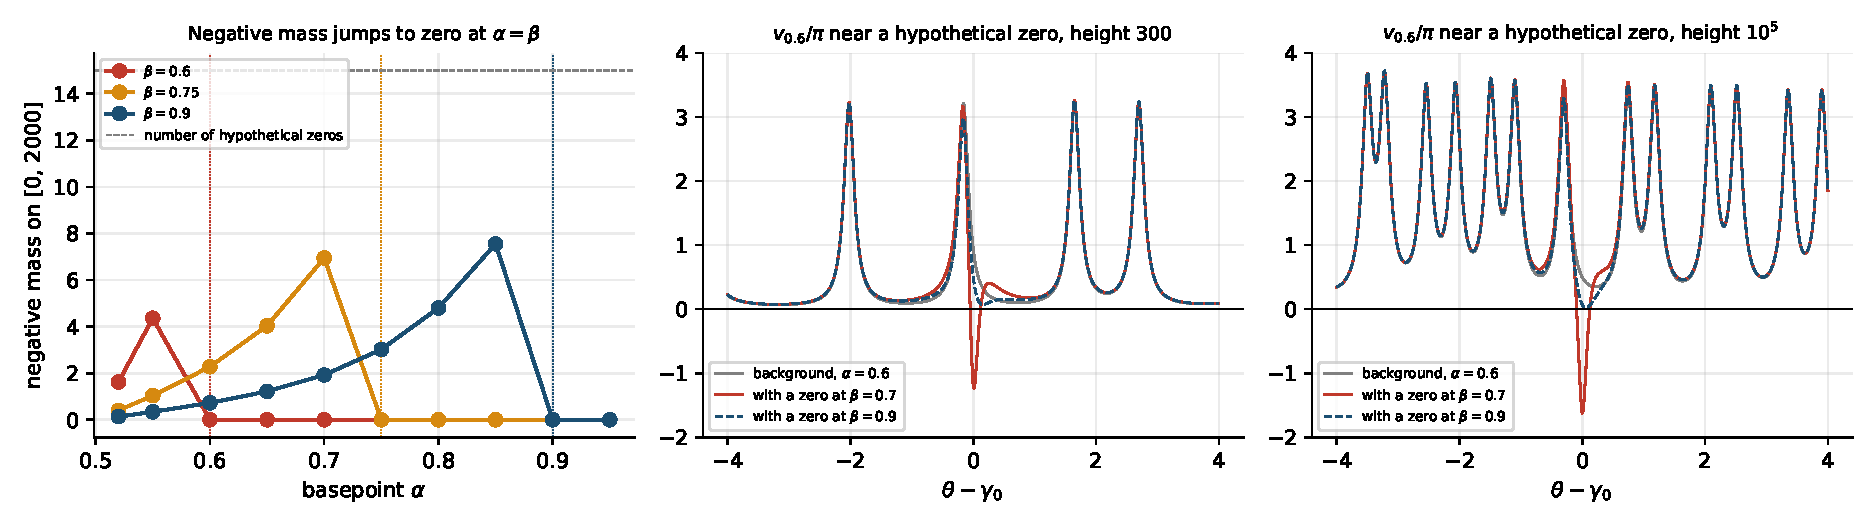
\includegraphics[width=\textwidth]{fig/ag_cancel.pdf}
\caption{Left: negative mass of the density on $[0,2000]$ against the basepoint $\alpha$ for fifteen hypothetical zeros at real part $\beta$ (\texttt{more2.py}). Middle and right: the density $v_{0.6}/\pi$ near the heights $300$ and $10^5$, alone and with a hypothetical pair of zeros at $\beta=0.7$ or $0.9$ at the centre of the window (\texttt{high.py}). Drawn by \texttt{figs\_almost.py}.}
\label{ag:fig:cancel}
\end{figure}

\begin{figure}[htbp]
\centering
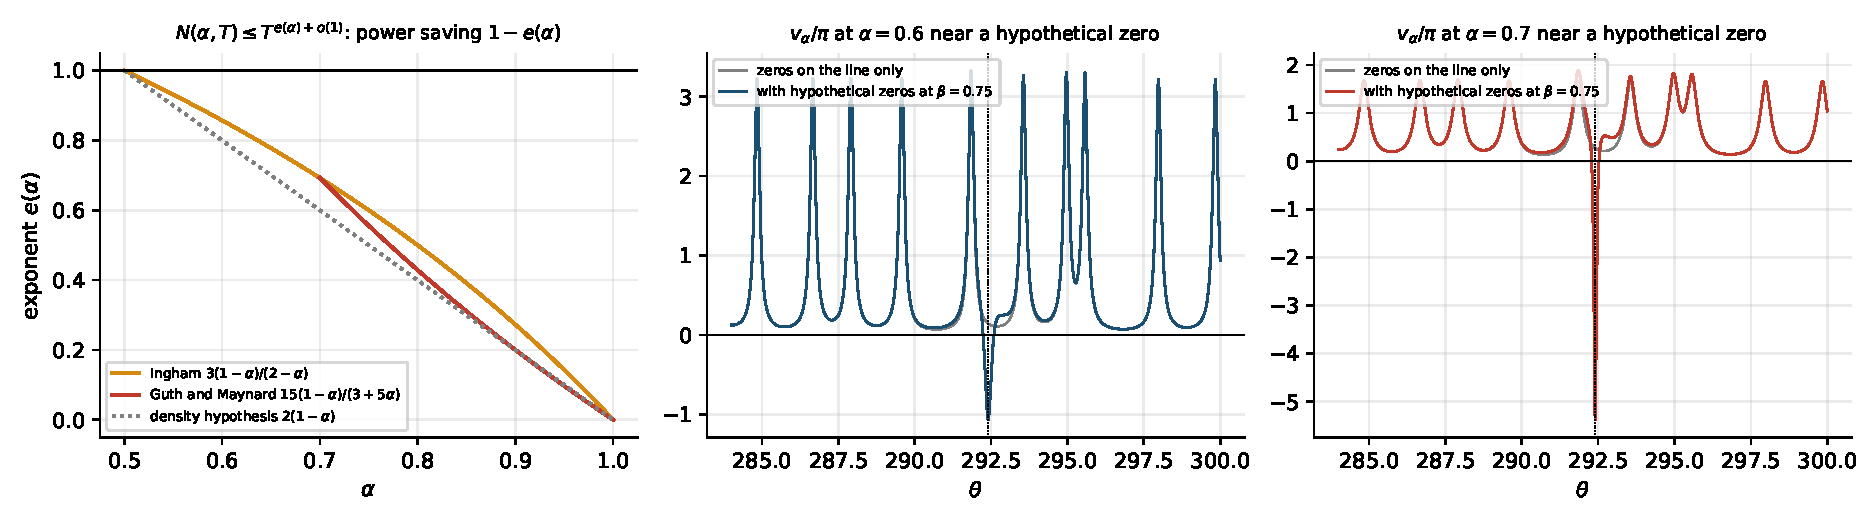
\includegraphics[width=\textwidth]{fig/ag_almost.pdf}
\caption{Left: the zero density exponents of Theorem~\ref{ag:thm:almost} and the region where they give a power saving; the exponent of Guth and Maynard is drawn on $[\frac7{10},1)$, where it holds by their estimate and, above $\frac45$, by Huxley's \cite{Huxley72}. Middle and right: the density $v_\alpha/\pi$ at $\alpha=0.6$ and $0.7$ near the hypothetical off line zero at height $292.4$ (dotted), with and without the hypothetical zeros, evaluated as in \texttt{almost.py} with step $0.005$. Drawn by \texttt{figs\_almost.py}.}
\label{ag:fig:almost}
\end{figure}

\subsection{Positivity margins and the circular unitary ensemble}\label{ag:sec:margins}

By Lemma~\ref{ag:lem:cancel}, a zero to the right of $\alpha$ at height $\gamma$ can make the density negative only if its distance to the line $\re s=\alpha$ is below $1/(\pi m)$, where $m$ is the local minimum of the rest of the density. The distribution of the local minima, the positivity margins, therefore determines how much room RH has at each height. The minima occur between consecutive ordinates. After unfolding the ordinates to unit mean spacing, $x_n=\vartheta(\gamma_n)/\pi+1$ with $\vartheta$ the Riemann Siegel theta function, as in Section~\ref{sec:ch15:spacings}, the density at the resolution of $\kappa$ mean spacings is
\[
\bar\rho_\kappa(x)=\sum_nP_\kappa(x-x_n)=\sum_n\frac{\kappa}{\pi(\kappa^2+(x-x_n)^2)},
\]
whose mean is one.

The script \texttt{sens.py} evaluates $\bar\rho_\kappa$ at the $1600$ midpoints between consecutive unfolded ordinates below height $2198$, leaving out $50$ mean spacings at each end, and the same statistic at about $3600$ midpoints between the eigenvalues of twelve Haar distributed unitary matrices of size $400$, unfolded and extended periodically. The circular unitary ensemble (CUE) of these matrices models the local statistics of the zeros. Table~\ref{ag:tab:margin} shows the result. The medians agree to $1\%$ at every resolution. In the lower tail the zeros have slightly larger margins than the CUE, a finite height effect in the expected direction, since the low zeros are more rigid than the limit of large matrices.

\begin{table}[htbp]
\centering\small
\begin{tabular}{ccccccc}
\toprule
$\kappa$ & zeta, 0.1\% & CUE, 0.1\% & zeta, 1\% & CUE, 1\% & zeta, median & CUE, median\\
\midrule
0.1 & 0.1075 & 0.0919 & 0.1177 & 0.1095 & 0.3349 & 0.3343\\
0.25 & 0.2617 & 0.2178 & 0.2849 & 0.2659 & 0.7116 & 0.7092\\
0.5 & 0.4803 & 0.4047 & 0.5150 & 0.4645 & 0.9739 & 0.9796\\
1 & 0.7477 & 0.6552 & 0.7730 & 0.7313 & 1.0264 & 1.0240\\
\bottomrule
\end{tabular}
\caption{Quantiles of the normalised Thorin density $\bar\rho_\kappa$ at the midpoints between consecutive unfolded ordinates, for the zeros below height $2198$ and for CUE eigenvalues. Computed by \texttt{sens.py}.}
\label{ag:tab:margin}
\end{table}

The next step is to repeat the comparison with Odlyzko's tables of zeros near the $10^{12}$th zero \cite{Odlyzko87} and near the $10^{21}$st and $10^{22}$nd zeros \cite{Odlyzko01,OdlyzkoTables}, where the finite height corrections are smaller, and to fit the lower tail of the margin distribution. The CUE lower tail is governed by large gaps, whose probability decays like a Gaussian in the gap length, so the smallest margin among the first $N$ midpoints should decrease only like a power of $\sqrt{\log N}$. Converted through the cancellation lemma, this predicts the width, as a function of the height, of the strip to the right of each basepoint in which an off line zero could hide without being cancelled. That is the quantitative input that question (1) of Section~\ref{ag:sec:exactly} needs.

\subsection{Moments of zeta, the Barnes function and zero density}\label{ag:sec:moments}

The strength of Theorem~\ref{ag:thm:almost} is set by the zero density exponents, which rest on mean value estimates on the critical line, Ingham's on the fourth moment of $\zeta$. Keating and Snaith \cite{KS00} modelled $\zeta(\frac12+it)$ by the characteristic polynomial $Z_N(\theta)=\det(I-Ae^{-i\theta})$ of a Haar distributed unitary matrix $A$ of size $N$, a matrix of the circular unitary ensemble of Section~\ref{ag:sec:margins}, with $N$ in the role of $\log(T/2\pi)$. By analogy with the exact formula
\[
\E|Z_N(\theta)|^{2k}=\prod_{j=1}^N\frac{\Gamma(j)\Gamma(j+2k)}{\Gamma(j+k)^2}\sim\frac{\mathsf G(1+k)^2}{\mathsf G(1+2k)}\,N^{k^2},\qquad N\to\infty,
\]
they conjectured that the moments of $\zeta$ grow in the same way, with $\log(T/2\pi)$ in place of $N$ and an arithmetic factor $a_k$ in front (Section~\ref{ag:sec:ks}). Here $\mathsf G$ is the Barnes $G$ function, $\mathsf G(1+z)=\Gamma(z)\mathsf G(z)$ with $\mathsf G(1)=1$, written in sans serif to keep $G$ for the clock of Section~\ref{ch:clock}. Nikeghbali and Yor \cite{NY09} gave the random matrix factor a probabilistic meaning in GGC language: the Mellin transform of $|Z_N|$ and the Barnes function are expressed through products and sums of independent gamma, beta and log gamma variables, and the reciprocal of $\mathsf G$ has a L\'evy Khintchine type representation. The source of these representations is the decomposition of Bourgade, Hughes, Nikeghbali and Yor \cite{BHNY08},
\[
Z_N\stackrel d=\prod_{j=1}^N\Big(1+e^{i\omega_j}\sqrt{B_{1,j-1}}\Big),
\]
with independent angles $\omega_j$ uniform on $[0,2\pi)$ and independent beta variables $B_{1,j-1}$ with parameters $1$ and $j-1$, where $B_{1,0}=1$.



\subsubsection{The Keating and Snaith moments}\label{ag:sec:ks}

Write $I_k(T)=\frac1T\int_0^T|\zeta(\frac12+it)|^{2k}dt$. The conjecture of Keating and Snaith \cite{KS00}, in the form of Conrey, Farmer, Keating, Rubinstein and Snaith \cite{CFKRS05}, is
\[
I_k(T)\sim a_k\,\frac{\mathsf G(1+k)^2}{\mathsf G(1+2k)}\Big(\log\frac T{2\pi}\Big)^{k^2},\qquad a_k=\prod_p\Big(1-\frac1p\Big)^{k^2}\sum_{m\ge0}\Big(\frac{\Gamma(m+k)}{m!\,\Gamma(k)}\Big)^2p^{-m},
\]
the product of an arithmetic factor from the primes and the random matrix factor. It is a theorem for $k=1$ and $k=2$ and open for $k\ge3$. For $k=1$ Hardy and Littlewood \cite{HL16} proved the leading term, and Ingham \cite{Ingham26} the mean square with its secondary term, $I_1(T)=\log\frac T{2\pi}+2\gamma_E-1+o(1)$; for $k=2$ Ingham \cite{Ingham26} proved the asymptotic with the leading coefficient $\frac1{2\pi^2}$. The local factor of $a_k$ is $(1-\frac1p)^{k^2}{}_2F_1(k,k;1;\frac1p)$. Since ${}_2F_1(1,1;1;x)=(1-x)^{-1}$ and ${}_2F_1(2,2;1;x)=(1+x)(1-x)^{-3}$, it equals $1$ for $k=1$ and $1-p^{-2}$ for $k=2$, so that $a_1=1$ and $a_2=\prod_p(1-p^{-2})=6/\pi^2$ exactly. The Euler product over the primes below $2\times10^5$ gives $a_3=0.0493218$ (\texttt{repro/ks\_ak.py}); since the local factor for $k=3$ is $1-9p^{-2}+O(p^{-3})$, the omitted primes lower it by a relative $9\sum_{p>2\times10^5}p^{-2}\approx4\times10^{-6}$, to about $0.0493217$. With $\mathsf G(3)^2/\mathsf G(5)=\frac1{12}$ and $\mathsf G(4)^2/\mathsf G(7)=\frac1{8640}$ the leading coefficients are $1$, $0.0506606=\frac1{2\pi^2}$, which is Ingham's constant, and $5.709\times10^{-6}$, the value $42a_3/9!$ of \cite{CFKRS05}.

Table~\ref{ag:tab:moments}, computed by \texttt{ks.py}, compares the moments with the leading terms. For $k=1$ the full asymptotic is already accurate at $T=1000$. For $k=2$ and $k=3$ the leading term is a small part of the moment at these heights, because the lower order terms of the polynomial in $\log T$ predicted in \cite{CFKRS05} dominate.

\begin{table}[htbp]
\centering\small
\begin{tabular}{ccccccc}
\toprule
$T$ & $I_1(T)$ & $\log\frac T{2\pi}+2\gamma_E-1$ & $I_2(T)$ & leading, $k=2$ & $I_3(T)$ & leading, $k=3$\\
\midrule
125 & 3.062 & 3.145 & 28.0 & 4.05 & 396 & 0.11\\
250 & 3.869 & 3.838 & 53.1 & 9.33 & 1136 & 0.71\\
500 & 4.550 & 4.531 & 84.8 & 18.6 & 2632 & 3.36\\
1000 & 5.211 & 5.224 & 127.2 & 33.5 & 5309 & 12.6\\
\bottomrule
\end{tabular}
\caption{Moments of $\zeta$ on the critical line against the asymptotic of Hardy, Littlewood and Ingham for $k=1$ and the leading Keating and Snaith terms for $k=2$ and $3$. Computed by \texttt{ks.py}.}
\label{ag:tab:moments}
\end{table}

\subsubsection{The moments as exponential moments of the Thorin density}

The densities $v_\sigma$ are the derivatives of $\log|\xi|$ across the basepoints: $\frac\partial{\partial\sigma}\log|\xi(\sigma+it)|=\re\frac{\xi'}{\xi}(\sigma+it)=v_\sigma(t)$ wherever $\xi(\sigma+it)\ne0$. Integrating from the critical line to the basepoint one, for every $t$ such that $\xi$ has no zero on the segment from $\frac12+it$ to $1+it$, which excludes only countably many $t$,
\begin{equation}\label{ag:eq:logxi}
\log|\xi(\tfrac12+it)|=\log|\xi(1+it)|-\int_{1/2}^1v_a(t)\,da .
\end{equation}
The moments concern $\zeta$, not $\xi$. With the gamma factor $h(s)=\frac12s(s-1)\pi^{-s/2}\Gamma(\frac s2)$, so that $\xi=h\zeta$, the identity becomes
\[
|\zeta(\tfrac12+it)|^{2k}=|\zeta(1+it)|^{2k}\,\Big|\frac{h(1+it)}{h(\frac12+it)}\Big|^{2k}\exp\Big\{-2k\int_{1/2}^1v_a(t)\,da\Big\},
\]
and Stirling's formula gives $|h(1+it)/h(\frac12+it)|\sim(t/2\pi)^{1/4}$ as $t\to\infty$. So the Keating and Snaith moments are exponential moments, over $t$ uniform on $[0,T]$, of the density $v_a(t)$ integrated across the basepoints from $\frac12$ to $1$, with the weight $|\zeta(1+it)|^{2k}|h(1+it)/h(\frac12+it)|^{2k}$, which involves no zero of $\zeta$. In the same terms, RH, which is the positivity of $v_a$ for every $a>\frac12$ (Lagarias's criterion, Remark~\ref{rem:ch2:oneline}), is the statement that $|\xi(\sigma+it)|$ increases with $\sigma\ge\frac12$ for every $t$, a reformulation due to Sondow and Dumitrescu \cite{SD10}.

In the language of \eqref{ag:eq:logxi} the conjecture of Keating and Snaith is a large deviation statement for the integrated Thorin density. Selberg's central limit theorem \cite{Selberg46} says that for $t$ uniform on $[T,2T]$ the variable $\log|\zeta(\frac12+it)|$ is approximately Gaussian with variance $\frac12\log\log T$. Gaussian exponential moments would give $(\log T)^{k^2}$, and the constant $a_k\mathsf G(1+k)^2/\mathsf G(1+2k)$ is the correction to them. On $[500,1000]$ the sample variance of $\log|\zeta(\frac12+it)|$ is $1.53$, against $\frac12\log\log750=0.95$. The difference is a constant term, not slow convergence: the random matrix model predicts the variance $\frac12\log\log\frac t{2\pi}+c+o(1)$ with $c=\frac12\big(\gamma_E+1-\sum_p\sum_{m\ge2}(\frac1m-\frac1{m^2})p^{-m}\big)=0.70$ \cite{KS00}, a conjecture, and this gives $1.48$ on $[500,1000]$, close to the sample value.

\subsubsection{What the moments give}

Ingham's exponent $3(1-\sigma)/(2-\sigma)$, which gives Theorem~\ref{ag:thm:almost} its saving $(2\alpha-1)/(2-\alpha)$ for $\frac12<\alpha<\frac7{10}$, rests on the fourth moment, $k=2$, proved by Ingham \cite{Ingham26}. Bounds for all moments, that is the Lindel\"of hypothesis in the form $\int_0^T|\zeta(\frac12+it)|^{2k}dt\ll T^{1+\varepsilon}$ for every $k$, imply the density hypothesis $N(\sigma,T)\ll T^{2(1-\sigma)+\varepsilon}$, which would give the saving $2\alpha-1$, larger than that of Theorem~\ref{ag:thm:almost} for $\frac12<\alpha<\frac9{10}$. The Keating and Snaith asymptotics would give this and much more.

The GGC structure of Nikeghbali and Yor belongs to the random matrix model, not to $\zeta$: it explains the conjecture without proving it, and only the second and fourth moments of $\zeta$ are known asymptotically. And moments, even the Lindel\"of hypothesis, bound the number of zeros off the line but do not exclude them.

\subsection{From almost to exactly}\label{ag:sec:exactly}

Theorem~\ref{ag:thm:almost} cannot be upgraded to exact positivity by improving the exponents, or by the moment bounds of Section~\ref{ag:sec:moments}. Even the density hypothesis, or the Lindel\"of hypothesis which implies it, leaves room for a sparse set of zeros off the line, and a single off line zero $\beta+i\gamma$ stops $T_\alpha$ from being a GGC for every $\alpha$ in $[\frac12,\beta)$ (Theorem~\ref{thm:poisson}) and makes $v_\alpha$ negative near $\gamma$ for every $\alpha$ close enough to $\beta$ (Section~\ref{ag:sec:cancel}). The step from ``almost'' to ``exactly'' is a step from counting zeros to excluding them.

Four facts about the programme say that this step needs input from outside it. The smoothing runs the wrong way: when no zero lies to the right of $\alpha$ the density at a basepoint $\alpha'>\alpha$ is the Poisson smoothing of the density at $\alpha$ by the kernel of width $\alpha'-\alpha$, and positivity propagates to the right; RH asks to propagate it to the left, which is deconvolution, and deconvolution does not preserve positivity. Arithmetic domination requires a zero free region: below the basepoint one the compensated L\'evy form, which the sine squared lemma converts into the density, holds if $\psi(x)-x=O(x^{\alpha'})$ for some $\alpha'<\alpha$, and only if $\psi(x)-x=O(x^{\alpha+\delta})$ for every $\delta>0$, where $\psi$ is Chebyshev's function (Proposition~\ref{bp:prop:below}). Either condition is a zero free half plane, none was known for any $\alpha<1$ before the half plane $\re s>\frac78$ announced in October 2026, which came from outside the programme (Section~\ref{sec:ch25:open}), and removing the pole does not help: for $L(s,\chi_{12})$ the prime sums need no compensation, and the boundary is the same (Section~\ref{bp:eta:sec:below}). There is no margin: along the de Bruijn Newman flow the reciprocal is a GGC for $t\ge0.2$ \cite{PT21} (Theorem~\ref{rz:thm:dbn} and Section~\ref{ch:dbn}), RH is the statement at $t=0$, and $\Lambda\ge0$ \cite{RodgersTao}, so a proof must establish a closed condition at the boundary itself. And stronger positivity conditions can be false: Conrey and Li showed that a positivity condition in de Branges' approach to RH fails \cite{CL00}, so any positivity statement stronger than RH should be tested numerically before it is pursued (Section~\ref{st:sec:wp5}).

In the Stieltjes form (iv) of Theorem~\ref{bh:thm:main} the difference between counting zeros and excluding them is explicit. Split $G'/G=S_{\rm on}+R_{\rm off}$, where $S_{\rm on}(u)=\sum(u+\gamma^2)^{-1}$ runs over the zeros $\frac12+i\gamma$ on the line with $\gamma>0$ and is a Stieltjes function with measure $U_{\rm line}$, and $R_{\rm off}(u)=\sum(u-(\rho-\frac12)^2)^{-1}$ runs over the zeros $\rho=\beta+i\gamma$ off the line with $\gamma>0$. By Theorem~\ref{bs:thm:local}, all the poles of $R_{\rm off}$ lie in a parabolic sliver $\mathcal E_{T_0}$ beside the negative axis, which begins at $-T_0^2+T_0+\frac14$, and in the upper half plane outside it $\im R_{\rm off}\le0$ and $\im(G'/G)<0$. The size of $R_{\rm off}$ away from the sliver needs no count of zeros: if $|u|\le T_0^2/2$, a disc that misses $\mathcal E_{T_0}$, then every term has $|u-(\rho-\frac12)^2|\ge|\rho-\frac12|^2-|u|>\gamma^2/2$, since $\gamma>T_0$, so $|R_{\rm off}(u)|\le2\Sigma_0<3\times10^{-12}$ by Theorem~\ref{ag:thm:explicit}.

The number of terms of $R_{\rm off}$, on the other hand, is not known to be small. Zero density estimates bound the number of those with $|\beta-\frac12|\ge\sigma-\frac12$ and $\gamma\le T$ by $T^{e(\sigma)+o(1)}$ with $e(\sigma)<1$, for each fixed $\sigma>\frac12$ (Theorem~\ref{ag:thm:almost}), which is $o(T)$; but zeros off the line may approach the line as $\gamma$ grows, and for all of them together only a proportion is known. At most $(1-\kappa+o(1))N(T)$ of the zeros up to height $T$ lie off the line, with $\kappa>\frac5{12}$ in the last published record \cite{PRZZ20} and $\kappa>0.6725$, counting only simple zeros on the line, in two preprints of 2026 \cite{AF26,Lam26}; that is not $o(T)$, nor even $o(N(T))$. No count, however strong, touches the Thorin condition, which requires $R_{\rm off}\equiv0$, because a single pair puts a pole of $G'/G$ off the cut. Section~\ref{pk:sec:filter} gives a test for arguments that claim to exclude such poles: since the de Bruijn Newman flow has nonreal zeros at every $t<0$ \cite{RodgersTao}, no property that the kernel $e^{tv^2/4}\Phi(v)$ keeps for some $t<0$ can exclude them, so a proof must use one that fails for every $t<0$, and the Euler product and the explicit formula are the natural candidates.

The forms that the new input could take are those of Section~\ref{ch:path}. The first new theorem any of them would give is the GGC property of $T_\alpha$ at a single basepoint $\alpha<\frac78$, that is $v_\alpha^-\equiv0$, a zero free half plane beyond the one announced in 2026 (Section~\ref{sec:ch25:open}); positivity of $v_\alpha$ on the single line $\re s=\alpha$ is not known to suffice (Remark~\ref{rem:ch2:oneline}).

Sections~\ref{ag:sec:factor} and \ref{ag:sec:cancel} make the remaining problem concrete. The growth of the defect is not part of it. For $u\ge1$ every factor of $D_\alpha$ is at most one, and a factor with $\gamma\le\sqrt u$ is at least $\gamma^2/(u+\gamma^2)\ge\gamma^2/(2u)\ge1/u$, since $\gamma\ge\gamma_1>\sqrt2$. Bounding the factors with $\gamma>\sqrt u$ as in the proof of Theorem~\ref{ag:thm:explicit} therefore gives, for $u\ge1$,
\begin{align*}
|\log D_\alpha(u)|&\le N(\alpha,\sqrt u)\log u+2(u+\sqrt u)\sum_{\beta>\alpha,\ \gamma>\sqrt u}\gamma^{-2}\\
&\le u^{e(\alpha)/2+o(1)},\qquad u\to\infty,
\end{align*}
by the exponents of Theorem~\ref{ag:thm:almost}. So bounds on the growth of the defect follow from zero density estimates alone, and what remains open is whether it is identically one. Four questions would each be a genuine step.
\begin{enumerate}
\item Cancellation on average: show that for fixed $\alpha>\frac12$ the background density $v_\alpha/\pi$ is bounded below by $c\log\gamma$ outside a set of heights of density zero. With Lemma~\ref{ag:lem:cancel} this would confine any failure of positivity to zeros in the strips $\alpha<\beta<\alpha+O(1/\log\gamma)$. Remark~\ref{rem:dbeta:average} proves the lower bound for $v_\alpha/\pi$ itself, but its exceptional set contains a neighbourhood of the ordinate of every zero to the right of $\alpha$, which is where Lemma~\ref{ag:lem:cancel} would need it.
\item Thin strip density: bound the number of zeros with $\alpha<\beta<\alpha+2/\log\gamma$ and $\gamma\le T$ by $o(T^{1-\delta})$ for some $\delta>0$, uniformly in $\alpha$. Combined with (1) this would give a pointwise almost positivity theorem.
\item Explicit defect: bound $\log D_\alpha(u)$ explicitly, as described at the end of Section~\ref{ag:sec:factor}.
\item Positivity at one basepoint: prove $D_\alpha\equiv1$, that is $v_\alpha^-\equiv0$, for a single $\alpha<\frac78$, which is a zero free half plane beyond the one announced in 2026 (Section~\ref{sec:ch25:open}).
\end{enumerate}
What the Thorin framework contributes is a precise target, the GGC property of one explicit clock $T_\alpha$ at one basepoint below $\frac78$, together with computational tools that test candidate arguments against it: certified densities on windows, positivity margins calibrated against random matrix theory, and the explicit defect. Chapter~\ref{chap:conclusions} takes stock of the whole path, beginning with Section~\ref{ch:path}.

\section{Pakes, the Lambert law and the Thorin condition}\label{sec:pakes}

Anthony Pakes has worked on the objects that surround the Thorin condition: size biasing and the classical moment problem, the Laplace transforms of positive infinitely divisible laws, the Lambert function, and ladders of self decomposable laws. This section follows the first author's account of that work and of what it gives for the clock \cite{P26pak}, verified, corrected where needed, and written in the notation of the book. In Pakes's language the question of Section~\ref{ch:ggc} is whether $\log G$ is a Thorin Bernstein function, that is, a Bernstein function whose L\'evy measure has the form $k(t)\,dt/t$ with $k$ completely monotone \cite[Chapter 8]{boSSV}, or equivalently the Laplace exponent of a GGC. By Theorem~\ref{bh:thm:main} this holds if and only if $(\log G)'=G'/G$ is a Stieltjes function, and if and only if RH holds. For the Lambert function $\mathcal W$ the corresponding statement, that $\mathcal W'$ is a Stieltjes function, is a theorem, and the Thorin measure of $\mathcal W$ is explicit. The section follows this parallel as far as it goes.

Section~\ref{pk:sec:strands} reviews the two strands of Pakes's work. Section~\ref{pk:sec:form} writes the Thorin question in his form: with no hypothesis the size biased clock is the clock plus an independent variable whose density is proportional to the heat trace, and RH holds exactly when this variable is a mixture of exponential laws; the moment problem of his first strand becomes the Hankel test of Section~\ref{ch:heat}, whose negative eigenvalues count the zeros off the line (Theorem~\ref{thm:ch12:inertia}), and Table~\ref{tab:ch21:nfaillong} follows the count along the de Bruijn Newman flow. Section~\ref{pk:sec:lambert} proves the theorem of Kalugin, Jeffrey and Corless that the Lambert law is a GGC with an explicit Thorin measure, by boundary values on the cut, reflection and a growth bound, and isolates the one step of that proof which does not transfer to the clock. The first author's account then localises, with no hypothesis, the points of the upper half plane where $\im(G'/G)$ could fail to be negative, as it must be for a Stieltjes function, to a thin parabola along the negative axis beyond about $-T_0^2$, where $T_0=3\times10^{12}$ is the height to which RH is verified; this is Lemma~\ref{bs:lem:disc} and Theorem~\ref{bs:thm:local} in Section~\ref{ch:boschB}, and what the zeros off the line could contribute there is discussed in Section~\ref{ag:sec:exactly}. Section~\ref{pk:sec:ladder} places the clock among Urbanik's multiply self decomposable laws, in $L_2$ and not in $L_3$ with no hypothesis, and shows that it is not the martingale limit of a supercritical continuous state branching process with finite Malthusian parameter. Section~\ref{pk:sec:filter} derives from the theorem of Rodgers and Tao a filter for the properties of the P\'olya kernel that could imply RH, and Section~\ref{pk:sec:assess} sorts what survives and lists open problems.

We do not prove RH, and several of the equivalences are elementary. What the section adds is a dictionary between Pakes's language and that of the book, a few unconditional facts about the clock, the solved Lambert problem as a template whose single failing step for the clock is RH itself, a list of routes that are closed, and one property, the GGC property of the variable of Biane, Pitman and Yor, that passes the filter of Section~\ref{pk:sec:filter} wherever it has been tested, but fails for most of the real Dirichlet $L$ functions tested there, so that it does not detect the Euler product. The programs \texttt{pakes\_sizebias.py} and \texttt{pakes\_lambert.py} compute the numbers of Sections~\ref{pk:sec:form} and \ref{pk:sec:lambert}.

\subsection{Two strands of Pakes's work}\label{pk:sec:strands}

The first strand is the classical moment problem. For a random variable $X\ge0$ with $0<\E X<\infty$, the size biased variable $\widehat X$, length biased in Pakes's word, has the law $x\,P(X\in dx)/\E X$. Pakes and Khattree \cite{PK92} characterise laws by in law equations linking $\widehat X$ and $X$, such as $X\stackrel d=\mathsf U\widehat X$ with $\mathsf U$ uniform on $(0,1)$ and independent of $\widehat X$, which holds exactly for the exponential laws, and they study the role of the moment problem in such characterisations, which can single out laws that are not determined by their moments. Pakes \cite{Pakes96} studies size biasing for the laws with the moments of the log normal law, and in \cite{Pakes01} he proves converse forms of the Carleman and Krein criteria and introduces size biasing and the stationary excess operation of order $r$; Berg \cite{Berg04} showed, correcting a remark in \cite{Pakes01}, that a law can be determinate in the sense of Stieltjes while its size biased and stationary excess versions of order one are not. Pakes, Hung and Wu \cite{PHW01} give criteria for the determination of a law by its moments, and Pakes \cite{Pakes07} describes the structure of the Stieltjes classes of moment equivalent laws; these papers are cited throughout the later literature on the moment problem, for instance by Stoyanov and his coauthors and by Penson and his coauthors.

Size biasing meets infinite divisibility in Steutel's theorem: $X$ is infinitely divisible if and only if $\widehat X\stackrel d=X+A$ for some $A\ge0$ independent of $X$, and the law of $A$ is then unique \cite{Steutel73}, \cite[Theorem 51.1]{Sato99}, \cite{SvH}; in this form the theorem is \cite[Theorem 11.1]{AGK19}, and Pakes takes it for positive laws from Pakes, Sapatinas and Fosam \cite{PSF96}. In Laplace transforms, with $\Psi(u)=-\log\E e^{-uX}$, it reads $\E e^{-u\widehat X}=\E e^{-uX}\,\Psi'(u)/\Psi'(0)$, so that $A$ has the Laplace transform $\Psi'(u)/\Psi'(0)$. In \cite{Pakes14} Pakes assumes the decomposition and asks when $A$ or $\widehat X$ is again infinitely divisible; he shows that size biasing up to the fourth order preserves infinite divisibility for the Lambert law and for a compound Poisson law, and conjectures that it does so at every order. Section~\ref{pk:sec:form} applies Steutel's theorem to the clock.

For the laws of this book the moment problem is determinate. The moment generating function $\xi(\frac12+z)/\xi(\frac12)$ of the P\'olya density is entire \eqref{eq:ch2:mgf}. The clock has $\E e^{sT}<\infty$ exactly for $s<\gamma_1^2=199.7904548\ldots$: every zero has $|\rho-\frac12|\ge|\im\rho|\ge\gamma_1$, so $1/G$ is analytic in the disc $|u|<\gamma_1^2$ and has a pole at $-\gamma_1^2$, and by Landau's theorem \cite[Chapter~II, Theorem~5b]{Widder41} the Laplace transform of a positive measure is singular at the real point of its abscissa of convergence, which is therefore $-\gamma_1^2$. Under RH the measure $\nu=\sum_ka_k^{-1}\delta_{1/a_k}$ of the Stieltjes moments $m_n$ is supported in $[0,\gamma_1^{-2}]$, so its moment problem is a determinate Hausdorff problem (Section~\ref{ch:heat}), while the Thorin measure $U_{\RH}$ itself has unbounded support and infinite mass.

The second strand concerns the Laplace transforms of positive infinitely divisible laws, and the Lambert function $\mathcal W$, the principal solution of $\mathcal W(u)e^{\mathcal W(u)}=u$ (Section~\ref{pk:sec:lambert}). Pakes \cite{Pakes11} and, independently, Kalugin and Jeffrey \cite{KJ10} proved that $\mathcal W$ is a Bernstein function, from a formula for the derivatives of $\mathcal W$ that involves a sequence of polynomials \cite[(8)]{Pakes26}: Pakes through the positivity of the polynomials, Kalugin and Jeffrey by showing that their coefficients form positive, log concave and unimodal sequences. So $e^{-\mathcal W(u)}=\mathcal W(u)/u$ is the Laplace transform of an infinitely divisible law, the Lambert law. In the same paper, by Pakes's own account \cite[Section 2]{Pakes26}, a complex variable argument shows that $\mathcal W'$ is a Stieltjes function, so that $\mathcal W$ is a Thorin Bernstein function and the Lambert law is a GGC. Kalugin, Jeffrey, Corless and Borwein \cite{KJCB12} obtained Stieltjes representations independently and showed that $\mathcal W$ is a complete Bernstein function; the distribution function of the Thorin measure of $\mathcal W$ is $\pi^{-1}\im\mathcal W(-y+i0)$, which vanishes for $y<1/e$ \cite{KJCB12}, \cite[Theorem 3.3]{KJC11}, and the Thorin representation itself is \cite[Theorem 6.2]{KJC11}, published, with integral representations of other types, in \cite{KJC12}. Pakes gave two further proofs that $\mathcal W$ is Thorin Bernstein: from Nuttall's integral for the coefficients $n^n/n!$ of $\mathcal W'$, which yields an explicit quantile function of the Thorin measure \cite{Pakes18}, and from continuous state branching processes, one of whose martingale limits has the cumulant function $\mathcal W$ \cite{Pakes20}, which also gives the self decomposability of the Lambert law.

In \cite{Pakes26} Pakes identifies the background driving L\'evy process of the Lambert law: it is compound Poisson with unit rate and jump density $\int ze^{-xz}\,U_{\mathcal W}(dz)$, where $U_{\mathcal W}$ is the Thorin measure of $\mathcal W$. With $T_{\mathcal W}$ a variable with the Lambert law and $J$ a jump of the driving process, this gives the in law relations $T_{\mathcal W}\stackrel d=\mathsf U(T_{\mathcal W}+J)$ and $T_{\mathcal W}\stackrel d=\mathsf U\,\mathcal SJ$, with $\mathsf U$ uniform on $(0,1)$, $\mathcal S$ the stationary excess operator and the factors on the right independent; and if both relations hold for a variable $X$ and some $J\ge0$ of finite mean $\mu>0$, then $X\stackrel d=\mu T_{\mathcal W}$, so that the two relations characterise the Lambert law up to a scale factor \cite[Theorem 1]{Pakes26} (Remark~\ref{pk:rem:sd}). He embeds the Lambert law in a family of GGCs whose Laplace transforms solve Lambert's trinomial equation \cite[Theorem 6]{Pakes26}, which gives one more proof that $\mathcal W$ is Thorin Bernstein \cite[Corollary 2]{Pakes26}, and he introduces BDLP ladders: from an infinitely divisible $X_0\ge0$ with $\E(\log(1+X_0))^n<\infty$ for every $n$, the law of $X_{n+1}$ is the self decomposable law driven by the L\'evy process of $X_n$ \cite[Section 5]{Pakes26}. In his indexing $X_1$ is self decomposable; this is a unit shift from Urbanik's classes $L_n$ used in Section~\ref{pk:sec:ladder}, in which $L_0$ is the class of self decomposable laws \cite{Urbanik73,Sato80,BergForst83}. Along a ladder he finds the size biased decomposition $\widehat X_{n+1}\stackrel d=X_{n+1}+A_n$, with $A_n$ of density proportional to the tail of the L\'evy measure of $X_n$ \cite[(53)]{Pakes26}, and this is the form in which Section~\ref{pk:sec:form} applies Steutel's theorem to the clock.

\subsection{The Thorin question in Pakes's form}\label{pk:sec:form}

For the clock the objects of both strands are at hand. The Thorin question asks whether $\log G$ is a Thorin Bernstein function, that is, whether $(\log G)'=G'/G$ is a Stieltjes function (Theorem~\ref{bh:thm:main}); then the Thorin measure is $U_{\RH}=\sum_{\gamma>0}\delta_{\gamma^2}$, with no drift (Proposition~\ref{prop:rigid}), and Stieltjes inversion \eqref{eq:ch3:inversion} recovers it from the boundary values of $G'/G$ on the cut, or, in integrated form, from those of $\log G$ (Section~\ref{sec:ch3:readings}). With no hypothesis, $\log G$ is a Bernstein function with L\'evy measure $W(t)\,dt/t$, where $W(t)=\sum_ke^{-a_kt}$ is the heat trace (Theorem~\ref{thm:ch12:idsd}); under RH, $W(t)=\int e^{-tz}\,U_{\RH}(dz)$, the counterpart for the clock of the formula that gives the canonical function of the Lambert law as the Laplace transform of the density of its Thorin measure (Corollary~\ref{pk:cor:levy}; \cite[(12)]{Pakes26}).

The Bernstein property is weaker than the Thorin Bernstein property, but it is not blind to the zeros off the line. A Bernstein function extends holomorphically to $\re u>0$, and the zeros $-a$ of $G$ that come from a zero $\rho=\frac12+\delta+i\gamma$ off the line have $\re(-a)=\delta^2-\gamma^2<0$, so holomorphy alone cannot see them. But the Bernstein property of $\log G$ says more, $W(t)\ge0$ for every $t>0$, and that would exclude, for instance, a zero off the line below all the other zeros: if $\re a=\gamma^2-\delta^2$ were smaller than $\re a_k$ for every other $a_k$, which is $\gamma_k^2$ for a zero on the line, the four zeros $\rho$, $1-\rho$, $\bar\rho$, $1-\bar\rho$ would contribute $2e^{-(\gamma^2-\delta^2)t}\cos(2\delta\gamma t)$ to $W(t)$, which dominates as $t\to\infty$ and changes sign. The property holds with no hypothesis (Theorem~\ref{thm:ch12:idsd}, whose proof uses the verification of RH below height $1000$), so it cannot decide RH; among the Bernstein functions it is the Thorin Bernstein property that is equivalent to RH.

Size biasing gives the Thorin question a form with one variable. The size biased clock $\widehat T$ has the law $t\,P(T\in dt)/\E T$, and $\E T=m_0=\sum_ka_k^{-1}=0.0231049931\ldots$, the first Stieltjes moment of Section~\ref{ch:heat}.

\begin{proposition}\label{pk:prop:sizebias}
With no hypothesis, $\widehat T\stackrel d=T+A$, with $A$ independent of $T$ and of density $W(t)/m_0$ on $(0,\infty)$. RH holds if and only if $A$ is a mixture of exponential laws, and then $A\stackrel d=E/V$, with $E$ standard exponential and independent of $V$, and $V$ of law $m_0^{-1}\sum_{\gamma>0}\gamma^{-2}\delta_{\gamma^2}$, the ordinates counted with multiplicity.
\end{proposition}

\begin{proof}
The Laplace transform of $\widehat T$ is
\[
\frac{\E[Te^{-uT}]}{m_0}=-\frac1{m_0}\,\frac d{du}\,\frac1{G(u)}=\frac1{m_0}\,\frac1{G(u)}\,\frac{G'}G(u).
\]
By Section~\ref{ch:clock}, $(G'/G)(u)=\int_0^\infty e^{-ut}W(t)\,dt$ for $u>0$ with no hypothesis, and $W>0$ (Theorem~\ref{thm:ch12:idsd}); letting $u\downarrow0$, monotone convergence gives $\int_0^\infty W(t)\,dt=(G'/G)(0)=G'(0)=\sum_ka_k^{-1}=m_0$. So $W/m_0$ is a probability density with Laplace transform $(G'/G)(u)/m_0$, the Laplace transform of $\widehat T$ is the product of those of $T$ and of a variable $A$ with this density, and by the uniqueness of Laplace transforms $\widehat T\stackrel d=T+A$ with $A$ independent of $T$. A variable $A>0$ is a mixture of exponential laws, $A\stackrel d=E/V'$ with $V'>0$ independent of $E$, exactly when it has a completely monotone density: the density of $E/V'$ is $\E[V'e^{-V't}]$, and conversely, by Bernstein's theorem, a completely monotone probability density is $\int_{[0,\infty)}e^{-vt}\,\sigma(dv)$ with $\int v^{-1}\sigma(dv)=1$, which forces $\sigma(\{0\})=0$, and this is the density of $E/V'$ with $P(V'\in dv)=v^{-1}\sigma(dv)$. The density $W/m_0$ is completely monotone exactly when RH holds (Section~\ref{ch:clock} and Table~\ref{tab:ch3:hierarchy}), and then $W(t)=\sum_{\gamma>0}e^{-\gamma^2t}=m_0\E[Ve^{-Vt}]$ with $V$ as stated.
\end{proof}

This is Steutel's decomposition of Section~\ref{pk:sec:strands} with $\Psi=\log G$, and it is the identity that Pakes derives along BDLP ladders \cite[(53)]{Pakes26}, here for the clock and the subordinator of Proposition~\ref{sb:prop:bdlp} that drives it, whose L\'evy density is $h=-W'$. Pakes's variable $A_n$ has the density $x\mapsto\int_x^\infty\omega_n(y)\,dy$, the tail of the L\'evy density $\omega_n$ of the driving law, normalised by the mean $\int_0^\infty x\,\omega_n(x)\,dx$, and for the clock the tail is $\int_t^\infty h(x)\,dx=W(t)$ and the mean is $\int_0^\infty xh(x)\,dx=\int_0^\infty W(t)\,dt=m_0$. The content of Proposition~\ref{pk:prop:sizebias}, RH if and only if $W$ is completely monotone, is that of Proposition~\ref{sb:prop:bdlp}; the size biased form puts it in one variable that exists with no hypothesis. Its mean is $\E A=m_1/m_0=\mathrm{Var}\,T/\E T=1.60885567\times10^{-3}$, from the Taylor coefficients of $\xi$ at $\frac12$, with no zero entering. Under RH, $A$ is infinitely divisible, as a mixture of exponential laws \cite{Goldie67,Steutel67}, and so is $\widehat T=T+A$; so under RH both parts of the question that Pakes asks in \cite{Pakes14} have a positive answer for the clock. The weights $P(V=\gamma^2)=\gamma^{-2}/m_0$ of the first six ordinates are $0.21663$, $0.09794$, $0.06919$, $0.04676$, $0.03990$ and $0.03064$: the lowest zero carries about a fifth of the law of $V$, and the first six carry $0.50105$, about a half. The first $1700$ ordinates carry $0.978508$. The rest is $m_0^{-1}\int_{(\gamma_{1700},\infty)}t^{-2}\,dN(t)$; the smooth part $\vartheta(t)/\pi+1$ of the count, with the boundary term $(\vartheta(\gamma_{1700})/\pi+1-1700)/(m_0\gamma_{1700}^2)$ that it leaves at $\gamma_{1700}$, accounts for it to within $3\times10^{-9}$, and the remainder is $2m_0^{-1}\int_{\gamma_{1700}}^\infty S(t)\,t^{-3}\,dt$, where $S(t)$ is the fluctuating part of the count. The program \texttt{pakes\_sizebias.py} computes these numbers, the moments at $80$ digits and the weights from the $70$ digit ordinates of \texttt{zeros\_1700.txt}, checked against mpmath's \texttt{zetazero}.

Pakes's first strand, the moment problem, enters through the Taylor coefficients at the origin. For $|u|<\gamma_1^2$ and for $|u|<1/e$ respectively,
\[
(\log G)'(u)=\sum_{n\ge0}m_n(-u)^n,\qquad \mathcal W'(u)=\sum_{n\ge1}\frac{n^n}{n!}(-u)^{n-1},
\]
with the Stieltjes moments $m_n=\sum_ka_k^{-n-1}$ of Section~\ref{ch:heat}; the second series is the derivative of the Lagrange series of $\mathcal W$ \cite[(3.1)]{Corless96}. Under RH, $m_{n-1}=\int z^{-n}\,U_{\RH}(dz)$ for $n\ge1$, just as $n^n/n!=\int z^{-n}\,U_{\mathcal W}(dz)$ (Corollary~\ref{pk:cor:nuttall}): both coefficient sequences are then moment sequences of positive measures, the images of $z^{-1}U_{\RH}(dz)$ and of $U_{\mathcal W}$ under $z\mapsto1/z$, and their Hankel matrices are positive definite. For $\mathcal W$ this is a consequence of the theorem of Section~\ref{pk:sec:lambert}. For the clock the positive definiteness of every $\mathcal H_N=[m_{i+j}]_{i,j<N}$ is equivalent to RH (Section~\ref{ch:heat}); the number of negative eigenvalues of $\mathcal H_N$ does not decrease with $N$ and tends to the number of distinct zeros $\rho$ with $\re\rho>\frac12$ and $\im\rho>0$ (Theorem~\ref{thm:ch12:inertia}); and Table~\ref{tab:ch21:nfaillong} shows the count at work along the de Bruijn Newman flow, where in the data a pair of zeros that starts at $(\gamma_k,\gamma_{k+1})$ is often registered soon after its collision at an order close to $2k+2$, although this rule fails at order $50$ (Section~\ref{sec:ch21:hankel}).

Li's criterion is a positivity condition on the same zeros, read on the Thorin functional through the test functions $\varphi_n$ of Section~\ref{sec:ch20:thorin}. It sees a zero off the line more slowly: the term of $\rho=\frac12-d+i\gamma$, with $0<d<\frac12$, grows like $e^{nd/\gamma^2}$, so it can dominate only from $n$ of order $\gamma^2/d$, which exceeds $2\gamma^2$, while in the data of Section~\ref{sec:ch21:hankel} the Hankel test often registers a pair at an order close to $2k+2$, set by its index $k$, at a cost in precision that grows linearly with the order (Section~\ref{ch:heat}). Both are tests at low height, and in both every zero off the line is eventually seen.

\subsection{The Lambert law, a Thorin problem solved}\label{pk:sec:lambert}

Let $\mathcal W$ be the principal branch of Lambert's function, the solution of $\mathcal W(u)e^{\mathcal W(u)}=u$ that is analytic on $\C\setminus(-\infty,-1/e]$, real and increasing on $(-1/e,\infty)$, with $\mathcal W(0)=0$, $\mathcal W(-1/e)=-1$ and $|\im\mathcal W|<\pi$. Its Lagrange series $\mathcal W(u)=\sum_{n\ge1}(-n)^{n-1}u^n/n!$ has radius $1/e$, and $\mathcal W(u)=\log u-\log\log u+o(1)$ as $u\to\infty$ \cite[(3.1), (4.19)]{Corless96}. Since $\mathcal W$ is a Bernstein function \cite{Pakes11,KJ10}, $e^{-\mathcal W(u)}=\mathcal W(u)/u$ is the Laplace transform of an infinitely divisible law on $[0,\infty)$, the Lambert law; we write $T_{\mathcal W}$ for a variable with this law. It is a GGC with an explicit, absolutely continuous Thorin measure, and the proof of this fact is a template that fails for the clock at exactly one step.

\begin{proposition}[{\cite[Section 4, (4.4)]{Corless96}}, {\cite[(10), (11)]{KJC11}}]\label{pk:prop:bv}
For $0<b<\pi$ put $r(b)=b\,e^{-b\cot b}/\sin b$. Then $r$ increases from $1/e$ to $\infty$ on $(0,\pi)$, and the boundary values of $\mathcal W$ on the cut, from the upper half plane, are $\mathcal W(-r(b)+i0)=-b\cot b+ib$.
\end{proposition}

\begin{proof}
Put $w=\alpha+ib$ with $0<b<\pi$ in $we^w=-x$, $x>0$. The imaginary part gives $e^\alpha(\alpha\sin b+b\cos b)=0$, so $\alpha=-b\cot b$, and then the real part gives $e^\alpha(\alpha\cos b-b\sin b)=-e^{-b\cot b}\,b/\sin b$, so that $x=r(b)$. Next, $(\log r)'(b)=1/b-2\cot b+b/\sin^2b$ and $b\sin^2b\,(\log r)'(b)=(b-\sin b\cos b)^2+\sin^4b>0$, while $r(0+)=1/e$ and $r(\pi-)=\infty$; so for each $x>1/e$ there is exactly one point $w$ of the curve $\{-b\cot b+ib:0<b<\pi\}$ with $we^w=-x$, namely the point with $r(b)=x$. This curve bounds the range of the principal branch in the upper half plane \cite[Section 4]{Corless96}, and $\mathcal W$ is continuous on the cut from above, with values on it; so $\mathcal W(-r(b)+i0)=-b\cot b+ib$.
\end{proof}

Kalugin, Jeffrey and Corless obtain the next theorem from the Stieltjes representation of $\mathcal W'$ \cite[Theorem 3.3]{KJC11} and the characterisation of Thorin Bernstein functions in \cite[Chapter 8]{boSSV}. The proof below is direct, by boundary values, reflection and a growth bound, and its four steps are compared with the clock at the end of the section.

\begin{theorem}[Kalugin, Jeffrey and Corless {\cite[Theorem 6.2]{KJC11}}, \cite{KJC12}]\label{pk:thm:lambert}
Let $U_{\mathcal W}$ be the image of the uniform law $db/\pi$ on $(0,\pi)$ under $r$, a probability measure on $(1/e,\infty)$. Then for $u\in\C\setminus(-\infty,-1/e]$
\[
\mathcal W(u)=\int\log\Big(1+\frac uz\Big)\,U_{\mathcal W}(dz)=\frac1\pi\int_0^\pi\log\Big(1+\frac u{r(b)}\Big)\,db .
\]
Hence $\mathcal W$ is a Thorin Bernstein function, and $T_{\mathcal W}$ is a GGC with no drift and Thorin measure $U_{\mathcal W}$, of total mass one, whose distribution function is $U_{\mathcal W}((1/e,y])=\pi^{-1}\im\mathcal W(-y+i0)$ for $y>1/e$.
\end{theorem}

\begin{proof}
Let $\Psi(u)$ be the integral. Since $U_{\mathcal W}$ is carried by $(1/e,\infty)$, $\Psi$ is analytic on $\C\setminus(-\infty,-1/e]$, real on $(-1/e,\infty)$, and $\Psi(\bar u)=\overline{\Psi(u)}$; so is $\mathcal W$. Let $x>1/e$, and let $b(x)\in(0,\pi)$ be the point with $r(b(x))=x$. As $\eta\downarrow0$, $1+(-x+i\eta)/z$ tends to a negative number from the upper half plane when $z<x$ and to a positive number when $z>x$, and $U_{\mathcal W}$ has no atoms, so by dominated convergence $\im\Psi(-x+i0)=\pi\,U_{\mathcal W}((1/e,x))=b(x)$; by Proposition~\ref{pk:prop:bv} also $\im\mathcal W(-x+i0)=b(x)$, which is the formula for the distribution function. Near $1/e$, $r(b)-1/e\sim b^2/(2e)$, so $U_{\mathcal W}$ has a density asymptotic to $(e/2)^{1/2}\pi^{-1}(z-1/e)^{-1/2}$ there, and a bounded continuous density on $[1/e+c,\infty)$ for every $c>0$. Hence $\Psi$ extends continuously to the closed upper half plane, and so does $\mathcal W$, with $\mathcal W(-1/e)=-1$. The difference $D=\mathcal W-\Psi$ is therefore continuous on the closed upper half plane and real on the real axis, where on $(-\infty,-1/e)$ the imaginary parts of the two boundary values agree. The Schwarz reflection principle continues $D$ across $(-\infty,-1/e)$, the continuation coincides with $D$ in the lower half plane because $D(\bar u)=\overline{D(u)}$, and the singularity at $-1/e$, where $D$ is bounded, is removable. So $D$ is entire, and $D(0)=0$.

It remains to bound $D$, and one sided bounds on real parts suffice. First, $\re\Psi(u)=\int\log|1+u/z|\,U_{\mathcal W}(dz)\le\log(1+e|u|)$, since $z>1/e$. Next let $|u|=R\ge e$ and $w=\mathcal W(u)$, so that $|w|e^{\re w}=R$ and $|\im w|<\pi$. If $|w|>\log R+\pi$, then $|\re w|>|w|-\pi>\log R$. This is impossible when $\re w\ge0$, since then $\re w=\log R-\log|w|<\log R$; and when $\re w<0$ it gives $\log|w|-\log R>|w|-\pi$, that is $|w|-\log|w|<\pi-\log R\le\pi-1$, which fails for $|w|>1+\pi$, since $x-\log x$ increases for $x>1$ and exceeds $\pi-1$ at $x=1+\pi$. Hence $|w|\le\log R+\pi$ and $\re\mathcal W(u)=\log R-\log|w|\ge\log R-\log(\log R+\pi)$. By continuity both bounds hold on the whole circle, its point on the cut included, so
\[
\max_{|u|=R}\re\big(-D(u)\big)\le\log(1+eR)-\log R+\log(\log R+\pi),\qquad R\ge e .
\]
The Borel Carath\'eodory lemma for the entire function $-D$, which vanishes at the origin, gives $\max_{|u|=R/2}|D(u)|\le2\max_{|u|=R}\re(-D(u))$, which is $O(\log\log R)$ by this bound. By Cauchy's estimates every Taylor coefficient of $D$ of positive order vanishes, so $D\equiv D(0)=0$.
\end{proof}

The growth step cannot be done by writing the integral as $\log u$ plus a bounded term. The total mass of $U_{\mathcal W}$ is one, but $\int\log z\,U_{\mathcal W}(dz)=\infty$, since $U_{\mathcal W}((y,\infty))\sim1/\log y$ as $y\to\infty$, and $\mathcal W(u)-\log u=-\log\log u+o(1)$ is unbounded; the one sided bounds avoid this.

\begin{corollary}[{first part from \cite[Theorem 6.5]{KJC11} and \cite{KJC12}}]\label{pk:cor:levy}
The canonical function of $T_{\mathcal W}$ is
\[
k_{\mathcal W}(x)=\int e^{-xz}\,U_{\mathcal W}(dz)=\frac1\pi\int_0^\pi e^{-x\,r(b)}\,db,
\]
so that $\mathcal W(u)=\int_0^\infty(1-e^{-ux})\,k_{\mathcal W}(x)\,dx/x$ for $u\ge0$. The symmetric law of $Z\sqrt{2T_{\mathcal W}}$, with $Z$ standard normal and independent of $T_{\mathcal W}$, has characteristic function $e^{-\mathcal W(w^2)}$, is an EGGC (Section~\ref{sec:ch3:hierarchy}), and has L\'evy density $k^{\rm s}_{\mathcal W}(|x|)/|x|$ with
\[
k^{\rm s}_{\mathcal W}(x)=\int e^{-x\sqrt z}\,U_{\mathcal W}(dz)=\frac1\pi\int_0^\pi e^{-x\sqrt{r(b)}}\,db,
\]
that is, $\mathcal W(w^2)=\int_0^\infty4\sin^2(wx/2)\,k^{\rm s}_{\mathcal W}(x)\,dx/x$ for real $w$.
\end{corollary}

\begin{proof}
Insert Frullani's integral $\log(1+u/z)=\int_0^\infty(1-e^{-ux})e^{-zx}x^{-1}dx$ in Theorem~\ref{pk:thm:lambert} and exchange the integrals by Tonelli's theorem. For the symmetric law, $\E e^{iwZ\sqrt{2T_{\mathcal W}}}=\E e^{-w^2T_{\mathcal W}}$, and the cosine dictionary \eqref{rz:eq:cosdict} with $U=U_{\mathcal W}$, for which $K_U=2k^{\rm s}_{\mathcal W}$, gives the L\'evy density $K_U(|x|)/(2|x|)$.
\end{proof}

\begin{remark}[Self decomposability, after Pakes]\label{pk:rem:sd}
Since $k_{\mathcal W}$ is nonincreasing, $T_{\mathcal W}$ is self decomposable, and as in Proposition~\ref{sb:prop:bdlp} its driving subordinator $\mathsf Z$ has the L\'evy density $-k_{\mathcal W}'(x)=\int ze^{-xz}\,U_{\mathcal W}(dz)$, of total mass $k_{\mathcal W}(0+)=1$ and with mean $\int_0^\infty k_{\mathcal W}(x)\,dx=\int z^{-1}\,U_{\mathcal W}(dz)=1$ (Corollary~\ref{pk:cor:nuttall}). So the driving process is compound Poisson with unit rate and jumps $J$ of mean one; its Laplace exponent is $u\mathcal W'(u)=\mathcal W(u)/(1+\mathcal W(u))$, and $\E e^{-uJ}=1/(1+\mathcal W(u))$ \cite[(5), (6), (18)]{Pakes26}. Stopping $T_{\mathcal W}=\int_0^\infty e^{-t}\,d\mathsf Z_t$ at the first jump of $\mathsf Z$, at an exponential time $\tau$, gives the perpetuity $T_{\mathcal W}\stackrel d=\mathsf U(T_{\mathcal W}+J)$, with $\mathsf U=e^{-\tau}$ uniform on $(0,1)$ and the three variables independent. The stationary excess $\mathcal SJ$ has the density $P(J>x)$, since $\E J=1$, and the Laplace transform $(1-\E e^{-uJ})/u=\mathcal W'(u)$; since $\E e^{-u\mathsf UY}=u^{-1}\int_0^u\E e^{-sY}ds$ for $Y\ge0$ independent of $\mathsf U$, also $T_{\mathcal W}\stackrel d=\mathsf U\,\mathcal SJ$, and $\mathcal SJ\stackrel d=J+T_{\mathcal W}$. The converse, part (b) of \cite[Theorem 1]{Pakes26}, has the same short proof, which we repeat in our notation. If $X\stackrel d=\mathsf U(X+J)$ and $X\stackrel d=\mathsf U\,\mathcal SJ$ for some $J\ge0$ of mean $\mu\in(0,\infty)$, put $\varphi(u)=\E e^{-uX}$, $j(u)=\E e^{-uJ}$ and $F(u)=u\varphi(u)$. The two relations say that $F'=\varphi j$ and $F'=(1-j)/(\mu u)$; eliminating $j=uF'/F$ gives $F'=F/(u(1+\mu F))$, so $y(u)=\mu F(u/\mu)$ satisfies $y'=y/(u(1+y))$, that is $(\log y+y)'=1/u$, with $y(u)\sim u$ as $u\downarrow0$. Hence $ye^y=u$ and $y=\mathcal W$ on $(0,\infty)$, which gives $\E e^{-uX}=\mathcal W(\mu u)/(\mu u)$, so $X\stackrel d=\mu T_{\mathcal W}$, and $j(u)=1/(1+\mathcal W(\mu u))$, so $J/\mu$ has the law of the jumps above.
\end{remark}

\begin{corollary}[{\cite[Corollary 3.4]{KJC11}}, \cite{KJCB12}; Nuttall's integral \cite{Nuttall85,Bouwkamp86}]\label{pk:cor:nuttall}
For $n\ge0$,
\[
\int z^{-n}\,U_{\mathcal W}(dz)=\frac1\pi\int_0^\pi\Big(\frac{\sin b\;e^{b\cot b}}b\Big)^n\,db=\frac{n^n}{n!}\qquad(0^0=1),
\]
so $(n^n/n!)_{n\ge0}$ is the moment sequence of the image of $U_{\mathcal W}$ under $z\mapsto1/z$, a probability measure on $(0,e)$. Nuttall conjectured, and Bouwkamp proved, the identity with $\nu^\nu/\Gamma(\nu+1)$ for every real $\nu\ge0$.
\end{corollary}

\begin{proof}
Differentiating Theorem~\ref{pk:thm:lambert} gives
\[
\mathcal W'(u)=\int\frac{U_{\mathcal W}(dz)}{u+z}=\sum_{n\ge1}(-u)^{n-1}\int z^{-n}\,U_{\mathcal W}(dz),\qquad |u|<1/e,
\]
the series converging uniformly in $z$ since $z>1/e$. Compare with the derivative of the Lagrange series $\mathcal W(u)=\sum_{n\ge1}(-n)^{n-1}u^n/n!$, whose coefficients are $(-n)^{n-1}/(n-1)!=(-1)^{n-1}n^n/n!$. For $n=0$ the integral is the total mass, one.
\end{proof}

Conversely, as Kalugin, Jeffrey and Corless observe after their Corollary 3.4 \cite{KJC11}, Nuttall's integral, which Bouwkamp proved without the Lambert function, gives back the theorem. It says that the image $\mu$ of $U_{\mathcal W}$ under $z\mapsto1/z$ has the moments $n^n/n!$, so $\int t\,\mu(dt)/(1+ut)=\int U_{\mathcal W}(dz)/(u+z)$ and $\mathcal W'(u)$ have the same Taylor series $\sum_{m\ge0}(-u)^m(m+1)^m/m!$ at the origin; both are analytic on $\C\setminus(-\infty,-1/e]$, so they agree, and integrating from $0$ gives Theorem~\ref{pk:thm:lambert}. Pakes's second proof that $\mathcal W$ is Thorin Bernstein also goes through Nuttall's integral \cite{Pakes18}, \cite[Section 2]{Pakes26}.

The program \texttt{pakes\_lambert.py} checks the section. At $40$ digits the boundary values of Proposition~\ref{pk:prop:bv} hold to $3\times10^{-40}$ at eight values of $b$ from $0.05$ to $3.1$ (at $30$ digits, at $b=1.3$, to all digits), the identity for $b\sin^2b\,(\log r)'$ holds to $10^{-39}$, and $(r(b)-1/e)/b^2$ is $0.18393972059$ at $b=10^{-6}$, against $1/(2e)$. The integral of Theorem~\ref{pk:thm:lambert} agrees with $\mathcal W$ to $2\times10^{-40}$ at seventeen points, ten real ones from $-0.3678$ to $10^{12}$ and seven complex ones, some next to the cut, such as $-5+0.001i$ and $-10^6+10^3i$. At $60$ digits Newton's method on $we^w=27/10$, the integral and Arb's Lambert function agree: $\mathcal W(2.7)=0.99662873426547746603029759804008309\ldots$. The binary double nearest $2.7$ exceeds $2.7$ by $1.8\times10^{-16}$, and $\mathcal W$ there is larger by $3.3\times10^{-17}$, so for digits beyond the sixteenth the input must be passed exactly, as the rational $27/10$. The moments of Corollary~\ref{pk:cor:nuttall} agree with $n^n/n!$ for $n\le12$ to $10^{-37}$, and with $\nu^\nu/\Gamma(\nu+1)$ at $\nu=0.5$, $1.5$, $2.7$ and $7.25$ to $3\times10^{-39}$; for $n=0,\dots,6$ they are $1$, $1$, $2$, $4.5$, $10.6667$, $26.0417$ and $64.8$. In double precision the L\'evy integrals of Corollary~\ref{pk:cor:levy} reproduce $\mathcal W(u)$ at $u=1$, $2.7$ and $10$, and $\mathcal W(w^2)$ at $w=1$ and $2$, to $6\times10^{-16}$, and $k_{\mathcal W}(x)$ is $0.988$ and $0.9988$ times $\sqrt{e/2}\,e^{-x/e}/\sqrt{\pi x}$ at $x=100$ and $1000$, as the density of $U_{\mathcal W}$ at $1/e$ predicts; at $z-1/e=1.8\times10^{-9}$ that density is $0.999999995$ times its asymptote. The growth facts behind the proof are visible too: $\mathcal W(u)-\log u+\log\log u$ falls from $0.308$ at $u=10^2$ to $0.0194$ at $10^{128}$; $U_{\mathcal W}((y,\infty))$ is $0.0290$ at $y=10^{16}$, against $1/\log y=0.0271$; and the part of $\int\log z\,U_{\mathcal W}(dz)$ from $b<\pi-c$ exceeds $\log(1/c)$ by $0.126$, $0.144$, $0.145$ and $0.145$ at $c=10^{-2}$, $10^{-4}$, $10^{-8}$ and $10^{-16}$. On the circles $|u|=R$ the lower bound $\re\mathcal W(u)\ge\log R-\log(\log R+\pi)$ of the proof holds with the margins $0.81$, $0.76$, $0.65$, $0.47$ and $0.30$ at $R=3$, $10$, $10^2$, $10^4$ and $10^8$, attained on the cut, and $|\mathcal W(u)|\le0.74(\log R+\pi)$ there.

What transfers to the clock. The proof of Theorem~\ref{pk:thm:lambert} has four steps: the boundary values on the cut, the positivity of the boundary measure, the identification by reflection and a growth bound, and, for the symmetric law, the cosine dictionary \eqref{rz:eq:cosdict}. For the clock the first step is the argument count. Continued along the upper side of the negative axis, past the zeros of $G$ on it by small half circles in the upper half plane, $\im\log G(-x+i0)=\pi N_{\rm line}(\sqrt x)$, where $N_{\rm line}(t)$ counts with multiplicity the zeros on the critical line with ordinate in $(0,t)$, because the four zeros $\rho$, $1-\rho$, $\bar\rho$, $1-\bar\rho$ of a zero off the line contribute to $G$ the factor $(1+u/a)(1+u/\bar a)=|1+u/a|^2>0$ at real $u$; so $N_{\rm line}(\sqrt x)$, the distribution function of $U_{\rm line}$ (Proposition~\ref{prop:struct}), is read from the boundary values of $\log G$ with no hypothesis, and it is $N(\sqrt x)$ under RH. The second step is then automatic, since a counting function is nondecreasing. The fourth step gives the Poisson trace $K_{1/2}(y)=\sum_ke^{-y\sqrt{a_k}}$, which is $\sum_{\gamma>0}e^{-\gamma y}$ under RH, as the L\'evy side of $Y_{1/2}=Z\sqrt{2T}$ (Section~\ref{sm:sec:poisson}), while the heat trace $W$ is the canonical function of $T$ itself (Section~\ref{sec:ch3:readings}); the two traces are linked with no hypothesis by subordination. The third step is the obstruction: $\mathcal W$ is analytic off $(-\infty,-1/e]$ by construction, whereas $\log G$ is analytic off $(-\infty,0]$ if and only if RH holds (Proposition~\ref{prop:rigid} and the argument after it). In the Lambert case the boundary measure is a continuum lying on the cut; for the clock its atoms are the zeros, and whether they all lie on the cut is the whole question.

\subsection{Multiply self decomposable laws and branching}\label{pk:sec:ladder}

The centre clock is self decomposable with no hypothesis (Theorem~\ref{thm:ch12:idsd}), so it is the integral $\int_0^\infty e^{-t}\,dZ_t$ of its driving subordinator $Z$ (Proposition~\ref{sb:prop:bdlp}). The law of $Z_1$ may be self decomposable in its turn, with a driving process of its own, and so on. Read upwards, from the last driving process to the clock, such a chain is what Pakes calls a BDLP ladder \cite[Section 5]{Pakes26}, after the background driving L\'evy process, and how far it goes places a law in one of Urbanik's classes $L_n$. This subsection shows that for the centre clock the chain has exactly three steps, with no hypothesis on the zeros (Theorem~\ref{pk:thm:ladder}), and that the clock is not the martingale limit of a supercritical continuous state branching process, the construction behind one of Pakes's proofs for the Lambert law (Theorem~\ref{pk:thm:nobranch}). Both obstructions come from the bottom of the spectrum: the ladder breaks at a time where the term of the first zero is negative and the other zeros cannot compensate it, and the branching relation breaks at a singularity that a numerical continuation traces to the critical point of $\Xi$ between the first two zeros. Neither says anything about RH. Along the de Bruijn Newman flow, where the zeros move towards the origin and apart, a computation that is numerical for $t>0$ keeps the index two on its window up to $t=27.8$ and finds the index one at $t=27.9$ and at every larger $t$ tested, by the same mechanism (Section~\ref{pk:sec:heatladder}).

\subsubsection{Urbanik's classes and the ladder functions}\label{pk:sec:urbanik}

A law $\mu$ on $\R$ is self decomposable if for every $c\in(0,1)$ there is a law $\mu_c$, the $c$ component of $\mu$, such that the characteristic functions satisfy $\widehat\mu(z)=\widehat\mu(cz)\,\widehat\mu_c(z)$. Urbanik \cite{Urbanik73} let $L_0$ be the class of self decomposable laws, $L_n$ for $n\ge1$ the class of laws in $L_{n-1}$ all of whose components lie in $L_{n-1}$, and $L_\infty=\bigcap_nL_n$. Sato \cite{Sato80} proved that $L_n$ is also the class of limit laws of normed sums of independent summands whose laws lie in $L_{n-1}$, and that $L_\infty$ is the smallest class of laws that contains the stable laws and is closed under convolution and weak limits \cite[Theorem 3.5]{Sato80}. In the language of Section~\ref{sb:sec:sd}, a law lies in $L_n$, $n\ge1$, exactly when it is self decomposable and the law at time one of its driving process lies in $L_{n-1}$ \cite{IJS04}. So $L_1$ consists of the self decomposable laws whose driving process is self decomposable, $L_2$ of those whose driving process has its law in $L_1$, and so on. Pakes counts the steps from one: his class $L^+_n$ consists of the drift free laws on $[0,\infty)$ in $L_{n-1}$, so that $L^+_1$ is the self decomposable class \cite{Pakes26}. We keep Urbanik's indexing.

For laws on $[0,\infty)$ Berg and Forst put the classes in analytic form. Let $f$ be the Laplace exponent of an infinitely divisible law $\mu$ on $[0,\infty)$, so that $\int e^{-ux}\,\mu(dx)=e^{-f(u)}$, and let $(Sf)(u)=uf'(u)$. Then $\mu\in L_n$ if and only if $Sf,S^2f,\dots,S^{n+1}f$ are Bernstein functions \cite[Theorem 1.3]{BergForst83}. For $n=0$ this says that $\mu$ is self decomposable exactly when $Sf$ is the Laplace exponent of a subordinator, its driving process, as in the proof of Proposition~\ref{sb:prop:bdlp}.

For the centre clock $f=\log G$, and $S$ acts on the canonical function $W$ through the ladder functions
\[
W^{[0]}=W,\qquad W^{[j+1]}(t)=-t\,\frac d{dt}W^{[j]}(t),\qquad\text{so that}\quad W^{[j]}=\Big(-t\frac d{dt}\Big)^jW .
\]
For one exponential, $(-t\frac d{dt})^je^{-at}=\beta_j(at)\,e^{-at}$, where $\beta_0=1$ and $\beta_{j+1}(u)=u\beta_j(u)-u\beta_j'(u)$:
\[
\beta_1(u)=u,\quad\beta_2(u)=u^2-u,\quad\beta_3(u)=u^3-3u^2+u,\quad\beta_4(u)=u^4-6u^3+7u^2-u .
\]
In general $\beta_j(u)=\sum_{i=1}^j(-1)^{j-i}S(j,i)\,u^i=(-1)^jB_j(-u)$, with $S(j,i)$ the Stirling numbers of the second kind and $B_j$ the Touchard polynomials, and since $\beta_j(u)e^{-u}=(-u\frac d{du})^je^{-u}$ and $-u\frac d{du}$ multiplies Mellin transforms by $s$,
\begin{equation}\label{pk:eq:mellin}
\int_0^\infty\beta_j(u)\,e^{-u}u^{s-1}\,du=s^j\,\Gamma(s)\qquad(s>0).
\end{equation}
The positive roots of $\beta_3$ are $(3\mp\sqrt5)/2=0.381966$ and $2.618034$, and those of $\beta_4$ are $0.165757$, $1.343380$ and $4.490864$, so that $\beta_4<0$ on $(0,0.165757)\cup(1.343380,4.490864)$. Since $W(t)=\sum_ke^{-a_kt}$ with $\re a_k\ge\gamma_k^2-\frac14>0$ for every zero (Section~\ref{sb:sec:sd}),
\begin{equation}\label{pk:eq:Wj}
W^{[j]}(t)=\sum_k\beta_j(a_kt)\,e^{-a_kt},
\end{equation}
the series converging absolutely and locally uniformly on $(0,\infty)$; the atoms of an off line zero come in conjugate pairs, so the sum is real.

\begin{lemma}\label{pk:lem:urbanik}
For every $j\ge0$ and $u\ge0$,
\begin{equation}\label{pk:eq:Sj}
\Big(u\frac d{du}\Big)^j\log G(u)=\int_0^\infty\big(1-e^{-ut}\big)\,W^{[j]}(t)\,\frac{dt}t .
\end{equation}
For $n\ge0$ the centre clock lies in $L_n$ if and only if $W^{[n+1]}\ge0$ on $(0,\infty)$, and then $W^{[1]},\dots,W^{[n]}$ are nonnegative too. In that case the driving processes $Z^{[1]}=Z$, $Z^{[2]}$, \dots, $Z^{[n+1]}$ exist, each the driving process of the law at time one of the one before; $Z^{[j]}$ has Laplace exponent $(u\frac d{du})^j\log G(u)$ and L\'evy density $W^{[j]}(t)/t$; and for $1\le j\le n$ the law of $Z^{[j]}_s$ is self decomposable for every $s>0$.
\end{lemma}

\begin{proof}
By \eqref{pk:eq:Wj}, $W^{[j]}(t)=O(t^je^{-\gamma_1^2t})$ as $t\to\infty$, and by the explicit formula \eqref{pk:eq:Wjarith} below, $W^{[j]}(t)=O(t^{-1/2}\log(1/t))$ as $t\downarrow0$. The case $j=0$ of \eqref{pk:eq:Sj} is the L\'evy Khintchine form of $\log G$ (Section~\ref{sb:sec:sd}). If it holds for $j$, then, since $ue^{-ut}=\frac d{dt}(1-e^{-ut})$,
\[
\begin{aligned}
u\frac d{du}\int_0^\infty\big(1-e^{-ut}\big)W^{[j]}(t)\,\frac{dt}t&=\int_0^\infty ue^{-ut}\,W^{[j]}(t)\,dt\\
&=\int_0^\infty\big(1-e^{-ut}\big)\,W^{[j+1]}(t)\,\frac{dt}t ,
\end{aligned}
\]
the boundary terms $(1-e^{-ut})W^{[j]}(t)$ vanishing at both ends by the two bounds. A function of the form \eqref{pk:eq:Sj} is a Bernstein function exactly when $W^{[j]}\ge0$: if $W^{[j]}\ge0$ it is a L\'evy Khintchine form, and conversely, if it is a Bernstein function, its derivative $\int_0^\infty e^{-ut}W^{[j]}(t)\,dt$ is completely monotone, hence the Laplace transform of a nonnegative measure, which by the uniqueness of Laplace transforms is $W^{[j]}(t)\,dt$. So by the theorem of Berg and Forst the clock lies in $L_n$ exactly when $W^{[1]},\dots,W^{[n+1]}$ are nonnegative. If $W^{[n+1]}=-t\,(W^{[n]})'\ge0$, then $W^{[n]}$ is nonincreasing, and since it tends to $0$ at infinity it is nonnegative; descending in the same way, so are $W^{[n-1]},\dots,W^{[1]}$. For the driving processes, the Laplace exponent of $\int_0^\infty e^{-t}\,dY_t$ is $\int_0^u\Psi_Y(w)\,dw/w$ when the subordinator $Y$ has Laplace exponent $\Psi_Y$ (proof of Proposition~\ref{sb:prop:bdlp}), so a self decomposable law with Laplace exponent $f$ has a driving process with Laplace exponent $uf'(u)$. Starting from $f=\log G$ and using \eqref{pk:eq:Sj}, $Z^{[j]}$ has Laplace exponent $(u\frac d{du})^j\log G$ and L\'evy density $W^{[j]}(t)/t$ for as long as the laws at time one are self decomposable, and the law of $Z^{[j]}_s$, with L\'evy density $sW^{[j]}(t)/t$, is self decomposable exactly when $W^{[j]}$ is nonincreasing \cite[Corollary 15.11]{Sato99}, that is, when $W^{[j+1]}\ge0$.
\end{proof}

For one exponential the second rung already fails: $W^{[2]}(t)=(a^2t^2-at)e^{-at}<0$ for $at<1$. So a gamma law, whose canonical function is a multiple of $e^{-at}$, is self decomposable but does not lie in $L_1$, and the question for the clock is whether the sum \eqref{pk:eq:Wj} over all zeros repairs the signs that each of its terms violates.

\subsubsection{The ladder index of the centre clock}\label{pk:sec:index}

\begin{theorem}\label{pk:thm:ladder}
Unconditionally, that is, using only the verification of RH below height $2197.3$ \cite{PT21}, $W^{[3]}(t)>0$ for every $t>0$, and $W^{[4]}(e^{-4.15})<0$. Consequently $W$, $W^{[1]}$ and $W^{[2]}$ are positive on $(0,\infty)$; the centre clock lies in $L_2$ and not in $L_3$; its driving process $Z=Z^{[1]}$ and the driving process $Z^{[2]}$ of $Z$ are self decomposable at every time, and the driving process $Z^{[3]}$ of $Z^{[2]}$ is self decomposable at no time.
\end{theorem}

\begin{proof}
By Lemma~\ref{pk:lem:urbanik} it suffices to prove the two inequalities; the lower ladder functions are then positive, not only nonnegative, since $W^{[j]}$ strictly decreases to $0$ when $W^{[j+1]}>0$. As in the proof of Theorem~\ref{thm:ch12:idsd}, large $t$ is handled with the zeros and small $t$ with the explicit formula, and the two ranges overlap.

Large $t$. Let $\tau_1=(3+\sqrt5)/(2\gamma_1^2)=0.0131039$, so that $\gamma_1^2\tau_1=2.618034$ is the largest root of $\beta_3$; beyond it $\beta_3$ is positive and increasing. The zeros with ordinates below $\Gamma=2197.3$ lie on the line \cite{PT21}; there are $N(\Gamma)=1700$ of them, the last at $2197.2587$, and \texttt{bdlp\_ladder.py} encloses each one in ball arithmetic. For $t\ge\tau_1$ each of them contributes $\beta_3(\gamma^2t)e^{-\gamma^2t}\ge0$ to $W^{[3]}(t)$, and the second contributes at least $\beta_3(\gamma_2^2\tau_1)e^{-\gamma_2^2t}>99.38\,e^{-\gamma_2^2t}$, since $\gamma_2^2\tau_1=5.7910$. A zero with ordinate $\gamma>\Gamma$, wherever it lies, has $\re a\ge\gamma^2-\frac14$ and $|a|\le\gamma^2+\frac14$, so its term has modulus at most $f(\gamma)=B_3((\gamma^2+\frac14)t)\,e^{-(\gamma^2-\frac14)t}$, where the Touchard polynomial $B_j$ has the moduli of the coefficients of $\beta_j$. Since $vB_j'(v)\le jB_j(v)$, the logarithm of $B_j(v)e^{-v}$ decreases at a rate of at least $\frac12$ for $v\ge2j$, so for $(\Gamma^2+\frac14)t\ge6$ the function $f$ decreases and $f(\gamma)\le f(\Gamma)e^{-(\gamma^2-\Gamma^2)t/2}$. Let
\[
N^+(T)=\frac T{2\pi}\log\frac T{2\pi e}+0.1038\log T+0.2573\log\log T+9.3675,
\]
an upper bound for $N(T)$ for $T\ge e$ \cite[Corollary 1.2]{HSW22}, whose derivative is at most $\frac1{2\pi}\log\frac T{2\pi}+\frac{0.4}T$ for $T\ge\Gamma$. Partial summation against $N\le N^+$, with $\gamma^2-\Gamma^2\ge2\Gamma(\gamma-\Gamma)$ and $\log\frac\gamma{2\pi}\le\log\frac\Gamma{2\pi}+\frac{\gamma-\Gamma}\Gamma$, bounds the sum of these moduli by
\[
\varepsilon(t)=f(\Gamma)\Big(N^+(\Gamma)-1700+\frac L{\Gamma t}+\frac1{2\pi\Gamma^3t^2}\Big),\qquad L=\frac1{2\pi}\log\frac\Gamma{2\pi}+\frac{0.4}\Gamma .
\]
The logarithmic derivative of $e^{\gamma_2^2t}\varepsilon(t)$ is at most $3/t-(\Gamma^2-\frac14-\gamma_2^2)<0$ for $t\ge\tau_1$, and $e^{\gamma_2^2\tau_1}\varepsilon(\tau_1)<10^{-27458}$. So $W^{[3]}(t)\ge e^{-\gamma_2^2t}\big(99.38-e^{\gamma_2^2t}\varepsilon(t)\big)>0$ for $t\ge\tau_1$.

Small $t$. Applying $(-t\frac d{dt})^j$ term by term to \eqref{eq:ch2:Warith}, which the Gaussian factors in $r$ and in $\log n$ allow, gives with no hypothesis
\begin{equation}\label{pk:eq:Wjarith}
W^{[j]}(t)=\beta_j\big(-\tfrac t4\big)e^{t/4}+A_j(t)-P_j(t),
\end{equation}
where
\begin{gather*}
A_j(t)=\frac1{2\pi}\int_0^\infty\beta_j(r^2t)\,e^{-r^2t}\,m(r)\,dr,\\
P_j(t)=\frac1{2\sqrt{\pi t}}\sum_{n\ge2}\frac{\Lambda(n)}{\sqrt n}\,e^{-v_n}q_j(v_n),\qquad v_n=\frac{(\log n)^2}{4t},
\end{gather*}
and $q_0=1$, $q_{j+1}(v)=(\frac12-v)q_j(v)+vq_j'(v)$, because $-t\frac d{dt}$ maps $t^{-1/2}$ to $\frac12t^{-1/2}$ and $v_n$ to $v_n$; thus
\[
q_3(v)=-v^3+\tfrac92v^2-\tfrac{13}4v+\tfrac18,\qquad q_4(v)=v^4-8v^3+\tfrac{29}2v^2-5v+\tfrac1{16} .
\]
In the notation of the proof of Theorem~\ref{thm:ch12:idsd}, $\frac1{2\pi}\int_0^\infty e^{-r^2t}\log\frac r{2\pi}\,dr=s_0(t)(\ell+\alpha_0)$, and since $-t\frac d{dt}$ multiplies $s_0$ by $\frac12$ and maps $\ell$ to $\frac12$, replacing $m(r)$ by $\log\frac r{2\pi}$ in $A_j$ gives
\[
\bar A_j(t)=2^{-j}s_0(t)\,(\ell+\alpha_0+j),
\]
which also follows from \eqref{pk:eq:mellin} and its derivative in $s$ at $s=\frac12$. For the difference we split the integral at $r=5$. For $r\le5$ we use $|\beta_j(u)|e^{-u}\le u$, valid for $j=2,3,4$ with equality only in the limit $u\downarrow0$, and the bound $\int_0^5r^2|m(r)-\log\frac r{2\pi}|\,dr<0.404$ stated after the proof of Theorem~\ref{thm:ch12:idsd}; for $r\ge5$ we use the bound $r^2|m(r)-\log\frac r{2\pi}|<0.05$ stated there, and substitute $u=r^2t$. This gives
\[
|A_j(t)-\bar A_j(t)|\le E_j(t)=\frac1{2\pi}\Big(0.404\,t+0.025\sqrt t\,J_j\Big),
\]
where $J_j=\int_0^\infty|\beta_j(u)|\,e^{-u}u^{-3/2}\,du$ satisfies $J_3<1.3313$ and $J_4<1.8295$. Let $\tau_2=1/75$. For $t\le\tau_2$ the main term $\bar A_3(t)$ decreases in $t$, because $-t\frac d{dt}\bar A_3=\bar A_4$ and $\ell+\alpha_0+4>0$; the modulus $|\beta_3(-\frac t4)|e^{t/4}$ of the polar term and $E_3(t)$ increase; and so does the modulus of each term of $P_3(t)$, because $v_n\ge v_2>9$, the polynomials $q_3$ and $q_4$ have no root in $[9,\infty)$, so that $q_3<0<q_4$ there, and $-t\frac d{dt}$ maps the $n$th term of $P_3$ to the $n$th term of $P_4$. At $t=\tau_2$ the four quantities are $\bar A_3(\tau_2)=0.357155$, $0.003378$, $E_3(\tau_2)<0.001469$, and at most $0.057882$ for the sum of the moduli of the terms of $P_3$, in which the terms with $n>200$ are bounded through $e^{-(\log n)^2/8t}\le n^{-\sigma}$, $\sigma=(\log200)/8t$, as in the proof of Theorem~\ref{thm:ch12:idsd}. Hence $W^{[3]}(t)>0.2944$ for $t\le\tau_2$, and since $\tau_2>\tau_1$, $W^{[3]}>0$ on $(0,\infty)$.

Rung four. Let $t_0=e^{-4.15}$. Then $\gamma_1^2t_0=3.1496$ lies in the interval $(1.343380,4.490864)$ on which $\beta_4<0$. The first five zeros contribute $-0.97604$, $0.62189$, $0.22811$, $0.01295$ and $0.00216$ to $W^{[4]}(t_0)$, and all zeros together, with the tail bound above, give $W^{[4]}(t_0)=-0.11089729616255\pm10^{-23}$ in ball arithmetic. The explicit formula confirms the sign without the zeros: at $t_0$ the polar term is $0.004066$, $\bar A_4(t_0)=0.228563$, $P_4(t_0)=0.344026$ and $E_4(t_0)<0.001928$, so that $W^{[4]}(t_0)<0.004066+0.228563+0.001928-0.344026<-0.109$.
\end{proof}

\begin{remark}\label{pk:rem:ladderproof}
(a) The large $t$ range can use the verification of RH below height $3\times10^{12}$ \cite{PT21} in place of the $1700$ zeros, with the crude bound $N(r)\le r^2$ for $r\ge200$ that Backlund's explicit form of the Riemann von Mangoldt formula gives \cite{Backlund}; the zeros above that height then contribute less than $e^{-10^{23}}$ for $t\ge\tau_1$, and \cite{HSW22} is not needed. (b) The constants $0.404$ and $0.05$ are computed, by \texttt{idsd\_height.py} and again by \texttt{bdlp\_ladder.py}, which finds $\int_0^5r^2|m(r)-\log\frac r{2\pi}|\,dr<0.40330$, $r^2|m(r)-\log\frac r{2\pi}|<0.0422$ on $[5,10]$ and, from Binet's formula with its leading terms cancelled, $<0.0462$ beyond. The second has an analytic replacement. Binet's formula \cite[(5.9.15)]{DLMF} at $z=\frac14+\frac{ir}2$, with the integral split at $v=r/4$ as in the proof of Theorem~\ref{thm:ch12:idsd}, gives for $r\ge5$
\[
r^2\Big|m(r)-\log\frac r{2\pi}\Big|\le\frac18+\frac12+\frac{4r^2}{3(3r^2-1)}+8r\,T_1\Big(\frac r4\Big)\le1.08,
\]
where $T_1(a)=\int_a^\infty v\,dv/(e^{2\pi v}-1)$, the four terms coming from $\log|z|$, from $\re\frac1{2z}$ and from the two parts of the integral, on which $|v^2+z^2|$ is at least $(3r^2-1)/16$ and at least $r/4$; none of them increases with $r$, and at $r=5$ they are $0.125$, $0.5$, $0.45045$ and $0.00348$. With $1.08$ in place of $0.05$ the proof goes through unchanged, with $W^{[3]}>0.28$ on $(0,\tau_2]$ and $W^{[4]}(t_0)<-0.090$. (c) The proof uses no zero above $\gamma_2$ except through the signs of their terms, no bound for $S(t)$ and no asymptotic argument. A second certificate in three ranges, in the same program, confirms the theorem: the zeros for $-\log t\le4.3348$; the explicit formula on $3700$ cells of width $0.001$ covering $4.30\le-\log t\le8$, where the least lower bounds are $0.3943$ for $W^{[2]}$ and $0.4096$ for $W^{[3]}$; and lower bounds $6.12$ for $W^{[2]}$ and $4.02$ for $W^{[3]}$ valid for every $t\le e^{-8}$.
\end{remark}

The ladder breaks where the first zero dominates. At $t_0$ its term, $\beta_4(3.1496)e^{-3.1496}=-0.97604$, is only partly cancelled by the others, which leave $W^{[4]}(t_0)=-0.11090$: the second zero, for which $\gamma_2^2t_0$ already exceeds the largest root $4.490864$ of $\beta_4$, contributes $0.62189$, and the zeros above it are too far out. On the arithmetic side the same failure is the prime $2$: its term in $P_4(t_0)$, $0.343448$, outweighs the archimedean main term $\bar A_4(t_0)=0.228563$. On $-\log t\in[0,10]$ a scan in double precision on a grid of step $0.001$, with the sign at the ends of every interval certified from the zeros, finds no negative value of $W$, $W^{[1]}$, $W^{[2]}$ or $W^{[3]}$, and finds $W^{[4]}<0$ exactly for $-\log t\in(3.946,4.335)$, $W^{[5]}<0$ on $(3.443,4.126)$ and $W^{[6]}<0$ on $(3.146,3.773)\cup(4.403,5.051)$. Every ladder function from the fourth on takes negative values, since $W^{[j+1]}\ge0$ would force $W^{[j]}\ge0$ (Lemma~\ref{pk:lem:urbanik}). Towards the origin the ladder functions approach fixed fractions of $W$: by \eqref{pk:eq:Wjarith}, $W^{[j]}(t)=\bar A_j(t)+O(1)$ as $t\downarrow0$, so that $W^{[2]}/W\to\frac14$ and $W^{[3]}/W\to\frac18$. The two ratios fall from $5.73$ and $5.95$ at $-\log t=4.30$ to $0.614$ and $0.404$ at $8$ and to $0.470$ and $0.291$ at $10$, decreasing throughout $[4.30,10]$, and the ratios of the main terms are $0.2879$ and $0.1535$ at $-\log t=32$. The least values of $W^{[2]}$ and $W^{[3]}$ on $4.30\le-\log t\le8$ are $0.396547$, at $4.30$, and $0.410976$, at $4.335$.

\begin{corollary}\label{pk:cor:unimodal}
With no hypothesis, for every $s>0$ the laws of $Z_s$ and of $Z^{[2]}_s$ are self decomposable, hence unimodal, and the law of $Z_s$ lies in $L_1$.
\end{corollary}

\begin{proof}
The first statement is Theorem~\ref{pk:thm:ladder} with Lemma~\ref{pk:lem:urbanik}, and Yamazato's theorem \cite{Yamazato78}, \cite[Theorem 53.1]{Sato99} gives unimodality. The Laplace exponent of $Z_s$ is $s\,u(\log G)'(u)$, so by \eqref{pk:eq:Sj} its images under $S$ and $S^2$ correspond to $sW^{[2]}$ and $sW^{[3]}$, which are positive, and the theorem of Berg and Forst places $Z_s$ in $L_1$.
\end{proof}

So Corollary~\ref{sb:cor:unimodal} extends from the clock to its first two driving processes, and Yamazato's theorem gives nothing further along the ladder, since $Z^{[3]}_s$ is not self decomposable.

\begin{remark}\label{pk:rem:Linf}
The centre clock is not in $L_\infty$, the closure of the stable laws under convolution and weak limits. This follows from Theorem~\ref{pk:thm:ladder}, since $L_\infty\subset L_3$, but it needs no computation. By \cite[Theorem 1.6]{BergForst83}, the Laplace exponents of the laws of $L_\infty$ on $[0,\infty)$ are the functions $\int_{(0,1]}u^\alpha\,\sigma(d\alpha)$ with $\sigma$ a finite measure. The atom of $\sigma$ at $\alpha=1$ is a drift, and for $\alpha<1$, $u^\alpha=\alpha\Gamma(1-\alpha)^{-1}\int_0^\infty(1-e^{-ut})\,t^{-\alpha}\,dt/t$. So a law of $L_\infty$ without drift has the canonical function $k(t)=\int_{(0,1)}\alpha\Gamma(1-\alpha)^{-1}t^{-\alpha}\,\sigma(d\alpha)$, which is at least $c/t$ for $t\ge1$, with $c=\int_{(0,1)}\alpha\Gamma(1-\alpha)^{-1}\,\sigma(d\alpha)>0$ unless the law is degenerate, while $W(t)$ decays like $e^{-\gamma_1^2t}$.
\end{remark}

\begin{remark}\label{pk:rem:perpetuity}
The perpetuity $T_{\mathcal W}\stackrel d=\mathsf U(T_{\mathcal W}+J)$ of Remark~\ref{pk:rem:sd} comes from a driving process that is compound Poisson, and the argument there applies to any such process: if the driving process $Y$ of a self decomposable law is compound Poisson with rate $c$ and jumps distributed as $J$, stopping $X=\int_0^\infty e^{-t}\,dY_t$ at the first jump gives $X\stackrel d=\mathsf U^{1/c}(X+J)$, with $\mathsf U$ uniform on $(0,1)$ and the three variables independent. The centre clock satisfies no relation of this form, for any $c>0$ and any $J\ge0$. Such a $J$ would have $\E\log(1+J)<\infty$, since $\log(1+\mathsf U^{1/c}J)\ge\log(1+J)+c^{-1}\log\mathsf U$ and $\E\log(1+\mathsf U^{1/c}J)\le\E\log(1+T)\le\E T=m_0$, and iterating the relation would write $T$ as $\int_0^\infty e^{-t}\,dY_t$ with $Y$ compound Poisson; but the driving process of a self decomposable law is unique in law, its Laplace exponent being $u(\log G)'(u)$, and that of the clock has the infinite L\'evy measure $-W'(x)\,dx$ (Proposition~\ref{sb:prop:bdlp}). Under RH, $-W'(x)=\sum_{\gamma>0}\gamma^2e^{-\gamma^2x}$ is a mixture of exponentials, as is the jump density $\int ze^{-xz}\,U_{\mathcal W}(dz)$ of the driving process $\mathsf Z$ of the Lambert law (Remark~\ref{pk:rem:sd}), but its total mass is infinite.
\end{remark}

The ladder of this subsection is not the derivative ladder of Theorems~\ref{thm:ch12:idsd}, \ref{thm:ch12:cm}, \ref{thm:ch12:cmint} and \ref{thm:ch12:window} and Table~\ref{tab:ch3:hierarchy}, which climbs the signs $c_k=(-1)^kW^{(k)}>0$. Its rungs are alternating combinations of the same $c_k$, with Stirling numbers as coefficients:
\begin{gather*}
W^{[j]}(t)=\sum_{i=1}^j(-1)^{j-i}S(j,i)\,t^ic_i(t),\\
W^{[3]}=t^3c_3-3t^2c_2+tc_1,\qquad W^{[4]}=t^4c_4-6t^3c_3+7t^2c_2-tc_1 .
\end{gather*}
Every rung of the derivative ladder is a consequence of RH, and the whole ladder, complete monotonicity of $W$, is RH. Of the BDLP ladder RH gives only the first rung, since a GGC is self decomposable; a gamma law is a GGC outside $L_1$, so the GGC property alone does not give $W^{[2]}\ge0$. In the other direction, $L_\infty$ lies inside the class of GGCs \cite[Section 4]{BergForst83}, so membership of the clock in $L_\infty$ would imply RH, but no finite rung does: for every $n$ the canonical function $(\log\frac1t)_+^n$, which vanishes on $[1,\infty)$ and so is not completely monotone, defines a law in $L_n$ that is not a GGC, its ladder functions being $n!/(n-j)!\,(\log\frac1t)_+^{n-j}$ for $j\le n$ and the measure $n!\,\delta_1(dt)$ for $j=n+1$. So rungs two and three of the BDLP ladder, which Theorem~\ref{pk:thm:ladder} proves, are unconditional facts about the shape of $W$, set by the first zeros and their spacing, and the ladder stops at a rung that says nothing about RH.

\subsubsection{The ladder along the de Bruijn Newman flow}\label{pk:sec:heatladder}

Theorem~\ref{rz:thm:dbn} places the centre clock in a family of laws. For every $t\ge\Lambda$, and so for every $t\ge0.2$ with no hypothesis, the function $R_t(u)=H_t(0)/H_t(2i\sqrt u)$ of Section~\ref{sec:ch21:flow} is the Laplace transform of a GGC whose Thorin measure has the atoms $a_k(t)=(z_k(t)/2)^2$, where $0<z_1(t)<z_2(t)<\cdots$ are the zeros of $H_t$, and $R_0=1/G$. Since $t$ now denotes the time of the flow, we write $x$ for the variable of the canonical function $W(x;t)=\sum_ke^{-a_k(t)x}$ of $R_t$, whose ladder functions are
\[
W^{[j]}(x;t)=\Big(-x\frac\partial{\partial x}\Big)^jW(x;t)=\sum_k\beta_j\big(a_k(t)x\big)\,e^{-a_k(t)x}.
\]
Lemma~\ref{pk:lem:urbanik} holds for these laws with the same proof, the bound for small $x$ now coming from the number of zeros of $H_t$, so the law with Laplace transform $R_t$ lies in $L_n$ exactly when $W^{[n+1]}(\cdot\,;t)\ge0$. The flow moves the zeros, and with them the index.

The program \texttt{heat\_ladder.py} computes $H_t$ by Gauss Legendre quadrature in ball arithmetic, its zeros on $(0,600]$ by a sign scan of step $0.2$ and bisection, and the ladder functions $W^{[j]}(x;t)$, $j\le5$, from these zeros on the fixed window $0\le-\log x\le8$, on a grid of step $0.001$, for nine values of $t$ (Table~\ref{pk:tab:heatladder}). Nothing needs computing for $-\log x\le0$: the largest roots of $\beta_2,\dots,\beta_5$ are $1$, $2.618034$, $4.490864$ and $6.510134$, and $a_1(t)x\ge a_1(t)\ge12.47$ in every row. The computation is numerical for $t>0$. The quadrature is checked against a rule with $1024$ nodes, with relative differences below $10^{-46}$ at $z=100$, $300$ and $590$, but its error is not bounded, and the zeros above $z=600$ are left out; an estimate from the density $\frac1{4\pi}\log\frac z{4\pi}$ of the zeros of $H_0$ puts their share of $W^{[3]}$ at $-\log x=8$ below $2\times10^{-9}$, and their share of $W^{[5]}$ below $10^{-5}$. At $t=0$ the computed zeros are the numbers $2\gamma_k$ to double precision, and there are $N(300)=138$ of them, the number that Arb's count of the zeros of $\zeta$ gives; $H_0$ agrees with $\Xi(z/2)/8$, computed from $\zeta$, to $10^{-46}$.

\begin{table}[htbp]
\centering\footnotesize
\begin{tabular}{rrrrrllc}
\toprule
$t$ & $z_1(t)$ & $a_2/a_1$ & $W^{[2]}/W$ & $W^{[3]}/W$ & $W^{[3]}<0$ & $W^{[4]}<0$ & $n$\\
\midrule
0 & 28.2695 & 2.2119 & 0.6144 & 0.4038 & none & $(3.946,4.335)$ & 2\\
0.2 & 28.1536 & 2.2142 & 0.6131 & 0.4029 & none & $(3.935,4.333)$ & 2\\
1 & 27.6920 & 2.2239 & 0.6078 & 0.3993 & none & $(3.893,4.321)$ & 2\\
4 & 25.9874 & 2.2678 & 0.5887 & 0.3864 & none & $(3.737,4.263)$ & 2\\
10 & 22.7127 & 2.3915 & 0.5545 & 0.3630 & none & $(3.426,4.090)$ & 2\\
20 & 17.7111 & 2.7188 & 0.5069 & 0.3301 & none & $(2.884,3.675)$ & 2\\
30 & 13.3727 & 3.2530 & 0.4687 & 0.3030 & $(2.983,3.343)$ & $(2.303,3.153)$ & 1\\
40 & 9.7966 & 4.0960 & 0.4374 & 0.2807 & $(2.236,3.014)$ & $(1.676,2.593)$ & 1\\
50 & 7.0629 & 5.3383 & 0.4115 & 0.2620 & $(1.563,2.539)$ & $(1.022,2.035)$ & 1\\
\bottomrule
\end{tabular}
\caption{The ladder functions of $R_t$ along the de Bruijn Newman flow, on the window $0\le-\log x\le8$: the first zero $z_1(t)$ of $H_t$, the ratio $a_2/a_1$ of the first two Thorin atoms, the ratios $W^{[2]}/W$ and $W^{[3]}/W$ at $-\log x=8$, the sets of $-\log x$ on which $W^{[3]}(x;t)<0$ and $W^{[4]}(x;t)<0$, to the grid step $0.001$, and the largest $n$ with $W^{[1]},\dots,W^{[n+1]}\ge0$ on the window: $R_t$ lies in no class above $L_n$, and in $L_n$ if the signs persist for $x<e^{-8}$. On the window $W$, $W^{[1]}$ and $W^{[2]}$ are positive and $W^{[5]}$ takes negative values for every $t$. Numerical for $t>0$; the row $t=0$ is Theorem~\ref{pk:thm:ladder}. Computed by \texttt{heat\_ladder.py}.}
\label{pk:tab:heatladder}
\end{table}

The row $t=0$ repeats from the zeros of $H_0$ what Theorem~\ref{pk:thm:ladder} proves for all $x$, with the interval on which $W^{[4]}<0$ found by the scan after it. Along the flow the zeros move towards the origin and apart: $z_1(t)$ falls from $28.27$ to $7.06$ at $t=50$, the ratio $a_2/a_1$ of the first two atoms rises from $2.21$ to $5.34$, and the number of zeros in $(0,600]$ rises from $138$ to $149$. The set on which $W^{[4]}<0$ follows the first atom to smaller values of $-\log x$. It lies where $a_1(t)x$ is in the interval $(1.343380,4.490864)$ on which $\beta_4<0$, less the part on which the other atoms compensate, and at $t=50$, where it covers most of that interval, the first atom alone almost decides the sign. Up to $t=20$ the third ladder function stays nonnegative on the window, and $R_t$ keeps the index two of the clock, as far as the window shows. Between $t=27.8$ and $t=27.9$ it turns negative. The program finds $W^{[3]}\ge0$ on the window at $t=21,\dots,27$ and $t=27.1,\dots,27.8$, which gives $W^{[2]}\ge0$ and $W^{[1]}\ge0$ there as well, by the descent in the proof of Lemma~\ref{pk:lem:urbanik} applied on $[e^{-8},\infty)$; at $t=27.9$ it finds $W^{[3]}<0$ for $3.230<-\log x<3.307$, with least value $-0.0015$, and at $t=30$, $40$ and $50$ on the intervals of the table. So, by this computation, for these $t$ the law with Laplace transform $R_t$, a GGC with no hypothesis, is not in $L_2$, and its index on the window drops to one. The mechanism is that of Theorem~\ref{pk:thm:ladder}, one rung lower: the term of the first atom in $W^{[3]}$ is negative where $a_1(t)x$ lies in $(0.381966,2.618034)$, and once the first two atoms are far enough apart the second no longer compensates it; at the threshold $a_2/a_1$ is between $3.113$ and $3.119$, against $2.212$ for the clock. At $t=50$ the ratio $W^{[2]}/W$, which for $t\le40$ decreases across the whole window, has an interior minimum, $0.276$ at $-\log x=2.682$: the same mechanism has begun to act on the second rung, which a single atom already violates.

Below the window the ratios $W^{[2]}/W$ and $W^{[3]}/W$ tend to $\frac14$ and $\frac18$, at $t=0$ by \eqref{pk:eq:Wjarith} and for every $t\ge0.2$ by the count of the zeros of $H_t$. For fixed $t>0$ the number $N_t(T)$ of zeros of $H_t$ in $(0,T]$ is $\Psi(T)+\frac t{16}\log T+O(1)$, with $\Psi(T)=\frac T{4\pi}\log\frac T{4\pi}-\frac T{4\pi}$: Ki, Kim and Lee proved a formula of this kind for every $t>0$ \cite[Theorem 1.4]{KKL09}, as recalled in \cite[Section 3]{RodgersTao}, and the Polymath project proved it in this form, with effective constants, for $0<t\le\frac12$ \cite[Theorem 1.5]{Polymath}. An error $O(\log T)$ would do. Partial summation against $d\Psi$, with the substitution $u=z^2x/4$ and \eqref{pk:eq:mellin} at $s=\frac12$, gives
\[
W^{[j]}(x;t)=\frac{\log(1/x)}{2^{j+3}\sqrt{\pi x}}\,\big(1+o(1)\big)\qquad(x\downarrow0),
\]
which at $t=0$ is the leading part of $\bar A_j$. The approach is slow: at the end of the window the two ratios are still between $0.41$ and $0.62$ and between $0.26$ and $0.41$. So for $t>0$ the signs below $x=e^{-8}$ are plausible but not proved, and the last column of the table gives the largest index that the window allows. Either way the index is set by the positions and the spacing of the first zeros: it changes along the flow where every law is a GGC with no hypothesis, and it carries no information about RH.

\subsubsection{No branching process realisation}\label{pk:sec:nobranch}

One of Pakes's proofs that $\mathcal W$ is a Thorin Bernstein function obtains the Lambert law as the limit of a branching process \cite{Pakes20} (Section~\ref{pk:sec:strands}). Let $Y$ be a spectrally positive L\'evy process with Laplace exponent $\Psi_Y(u)=-\log\E e^{-uY_1}$, with the sign of Proposition~\ref{sb:prop:bdlp}, and with finite Malthusian parameter $\Psi_Y'(0)\in(0,\infty)$. Lamperti's time change turns $Y$ into a continuous state branching process $(\mathsf B_t)_{t\ge0}$; started at $\mathsf B_0=z>0$ it has $\E\mathsf B_t=ze^{\Psi_Y'(0)t}$, and the nonnegative martingale $e^{-\Psi_Y'(0)t}\mathsf B_t$ converges almost surely to a limit $\mathsf M$. By the branching property $\E e^{-u\mathsf M}=e^{-z\omega(u)}$ for a function $\omega$ that does not depend on $z$. Conditioning on $\mathsf B_s$ gives $\omega(u)=v_s\big(\omega(ue^{-\Psi_Y'(0)s})\big)$, where $e^{-zv_s(\theta)}=\E e^{-\theta\mathsf B_s}$ and $\partial_sv_s=\Psi_Y(v_s)$, and differentiating at $s=0$ gives
\begin{equation}\label{pk:eq:branch}
\Psi_Y'(0)\,u\,\omega'(u)=\Psi_Y\big(\omega(u)\big),
\end{equation}
which is \cite[(68)]{Pakes26}. For the Lambert law, $Y$ is the compound Poisson process with unit rate and standard exponential jumps, $\Psi_Y(u)=u/(1+u)$ and $\Psi_Y'(0)=1$, and $\omega=\mathcal W$ solves \eqref{pk:eq:branch}, since differentiating $\mathcal We^{\mathcal W}=u$ gives $u\mathcal W'=\mathcal W/(1+\mathcal W)$ \cite[Section 7]{Pakes26}.

For the centre clock, or $\lambda T$ with $\lambda>0$, to be such a limit we need $z\omega(u)=\log G(\lambda u)$. Then \eqref{pk:eq:branch} determines $\Psi_Y$ on the range $[0,\infty)$ of $\omega$:
\[
\Psi_Y(w)=\frac{\Psi_Y'(0)}z\,g(zw),\qquad g=\Psi_Z\circ H=\frac H{H'},
\]
where $H$ is the inverse function of $\log G$ and $\Psi_Z(u)=u(\log G)'(u)$ is the Laplace exponent of the driving process of Proposition~\ref{sb:prop:bdlp}. The function $g$ is analytic at $0$, with $g(w)=\sum_{k\ge1}g_kw^k$ and $g_1=1$. For every spectrally positive $Y$ the function $-\Psi_Y''(u)=\sigma^2+\int_0^\infty x^2e^{-ux}\,\Pi(dx)$, with $\sigma^2$ the Gaussian coefficient and $\Pi$ the L\'evy measure of $Y$, is completely monotone (and if $Y$ is a subordinator, so is $\Psi_Y'$). Since $\Psi_Y^{(k)}(0)=\Psi_Y'(0)\,z^{k-1}k!\,g_k$, this forces
\begin{equation}\label{pk:eq:pattern}
(-1)^{k-1}g_k\ge0\qquad(k\ge2).
\end{equation}
The coefficients $g_k$ need no hypothesis. The Taylor series of $\xi$ at $\frac12$, computed in ball arithmetic, gives that of $\log G(u)=\log\xi(\frac12+\sqrt u)-\log\xi(\frac12)=\sum_{n\ge1}(-1)^{n+1}m_{n-1}u^n/n$, with the Stieltjes moments $m_n=\sum_ka_k^{-n-1}$ of Section~\ref{ch:heat}; reverting the series gives $H$, and composing gives $g=\Psi_Z\circ H$. The program \texttt{branch\_coeffs.py} does this at $3200$ bits for $k\le60$, checks it against the second route $g=H/H'$, which agrees for $k\le59$ (the last coefficient is cut by the length of the series), and checks $m_1,\dots,m_{11}$ against the sums over the first $1700$ zeros. Every sign for $k\le60$ is certified, and Table~\ref{pk:tab:gk} lists the first thirty coefficients.

\begin{table}[htbp]
\centering\footnotesize
\begin{tabular}{rlrl}
\toprule
$k$ & $g_k$ & $k$ & $g_k$\\
\midrule
1 & $1$ & 16 & $1.49524474945\times10^{-15}$\rlap{$^*$}\\
2 & $-3.48161903048\times10^{-2}$ & 17 & $-5.70288794250\times10^{-16}$\rlap{$^*$}\\
3 & $5.36818625476\times10^{-3}$ & 18 & $9.65518218408\times10^{-17}$\rlap{$^*$}\\
4 & $-8.70698237260\times10^{-4}$ & 19 & $-1.21432018700\times10^{-17}$\rlap{$^*$}\\
5 & $1.36973198860\times10^{-4}$ & 20 & $1.16783296302\times10^{-18}$\rlap{$^*$}\\
6 & $-2.05209454841\times10^{-5}$ & 21 & $-6.77018656749\times10^{-20}$\rlap{$^*$}\\
7 & $2.91586074297\times10^{-6}$ & 22 & $-3.60435568970\times10^{-21}$\\
8 & $-3.92530248114\times10^{-7}$ & 23 & $1.93592106401\times10^{-21}$\\
9 & $4.99813541563\times10^{-8}$ & 24 & $-3.85744224396\times10^{-22}$\\
10 & $-5.99595770666\times10^{-9}$ & 25 & $5.68747574953\times10^{-23}$\\
11 & $6.72224097409\times10^{-10}$ & 26 & $-6.72011823221\times10^{-24}$\\
12 & $-6.93358579492\times10^{-11}$ & 27 & $6.03459570343\times10^{-25}$\\
13 & $6.37029732062\times10^{-12}$ & 28 & $-2.66337804089\times10^{-26}$\\
14 & $-4.81096482192\times10^{-13}$ & 29 & $-4.09850045758\times10^{-27}$\rlap{$^*$}\\
15 & $2.15183811282\times10^{-14}$ & 30 & $1.42466491988\times10^{-27}$\rlap{$^*$}\\
\bottomrule
\end{tabular}
\caption{The Taylor coefficients of $g=\Psi_Z\circ H$, the only candidate, up to scaling, for the Laplace exponent of a generating process of the centre clock (Theorem~\ref{pk:thm:nobranch}), to twelve digits; a star marks a sign that violates \eqref{pk:eq:pattern}. Every digit shown is certified in ball arithmetic at $3200$ bits from the Taylor series of $\xi$ at $\frac12$, and the signs are certified for $k\le60$: the wrong signs are those with $16\le k\le21$, $29\le k\le35$, $43\le k\le49$ and $56\le k\le60$. Computed by \texttt{branch\_coeffs.py}.}
\label{pk:tab:gk}
\end{table}

\begin{theorem}\label{pk:thm:nobranch}
With no hypothesis, $(-1)^{15}g_{16}<0$: in ball arithmetic $g_{16}=1.49524474945112\times10^{-15}\pm2\times10^{-30}$. Consequently no positive multiple of the centre clock is the martingale limit of a supercritical continuous state branching process with finite Malthusian parameter, from any initial state.
\end{theorem}

\begin{proof}
Such a limit would satisfy \eqref{pk:eq:pattern}, which the sign of $g_{16}$ violates.
\end{proof}

Theorem~\ref{pk:thm:nobranch} needs only one certified sign, but the signs fail for a structural reason, and they keep failing. The reason is Pringsheim's theorem, the power series form of Landau's theorem \cite[Chapter~II, Theorem~5b]{Widder41}: if $(-1)^{k-1}g_k\ge0$ for all large $k$ and the series $\sum g_kw^k$ has a finite radius of convergence $R$, then its sum is singular at $w=-R$. But $g$ is analytic on a neighbourhood of the negative axis. With no hypothesis, $(\log G)'(u)=\sum_k1/(u+a_k)>0$ for $-\gamma_1^2<u\le0$: a zero on the line contributes $1/(u+\gamma^2)>0$, and the conjugate atoms $a$, $\bar a$ of an off line zero together contribute $2\re(u+a)/|u+a|^2$, with $\re(u+a)\ge\gamma^2-\frac14-\gamma_1^2>0$. At $u=-1$, $-100$, $-190$, $-199$ and $-199.7$ the derivative is $0.02314$, $0.02957$, $0.1236$, $1.287$ and $11.08$. So $\log G$ increases from $-\infty$ to $0$ on $(-\gamma_1^2,0]$, its inverse $H$ is analytic on a neighbourhood of $(-\infty,0]$, and so is $g=H/H'$. Hence \eqref{pk:eq:pattern} fails for infinitely many $k$ unless $g$ is entire.

Numerically the radius is finite, $R=7.1565$, and the singularities that fix it lie off the axis. The function $\Xi$ has a critical point $t^*=15.5857085898$ between $\gamma_1$ and $\gamma_2$, certified by bisection on $\Xi'$, and at $u^*=-t^{*2}=-242.914312$ the function $G(u)=\Xi(\sqrt{-u})/\Xi(0)$ has $G'(u^*)=0$ and $G(u^*)=-0.00161241048$. Continued from $0$ around the zero $-\gamma_1^2$ through the upper half plane, $\log G$ reaches $u^*$ with the value
\[
\lambda^*=\log|G(u^*)|+i\pi=-6.43002502663+i\pi,
\]
of modulus $|\lambda^*|=7.156453$ and argument $\arg\lambda^*=2.687121$, and since $(\log G)'(u^*)=0$, the inverse $H$ has a square root branch point at $\lambda^*$, and by symmetry at $\bar\lambda^*$. Continuing $H$ numerically along the segment from $0$ to $\lambda^*$ in $3000$ steps keeps $|G|=e^{\re\lambda}\ge0.0016$ on the path, away from the zeros of $G$, and brings the preimage to within $2.86$ of $u^*$, at a distance proportional to the square root of the distance from $\lambda^*$ over the last steps, as at a simple critical point; so $\lambda^*$ and $\bar\lambda^*$ are singularities of the principal branch of $g$ (a numerical continuation, not a certificate). The root test agrees: $|g_k|^{1/k}$ is $0.1269$, $0.1274$, $0.1296$, $0.1288$ and $0.1317$ at $k=20$, $30$, $40$, $50$ and $60$, approaching $1/|\lambda^*|=0.13973$ slowly, as the factor $k^{-3/2}$ of a square root singularity predicts, while the consecutive ratios $|g_{k+1}/g_k|$, between $0.120$ and $0.162$ for $2\le k\le9$, swing from $0.005$ to $3.2$ beyond, near each change of sign. The conjugate pair makes $(-1)^{k-1}g_k$ oscillate in $k$ with period $2\pi/(\pi-\arg\lambda^*)=13.8253$, and the certified wrong signs come in the blocks of Table~\ref{pk:tab:gk}, at spacings $13$, $14$ and $13$.

The next critical points of $\Xi$ do not matter. The second, $t^{**}=22.0979772804$ between $\gamma_2$ and $\gamma_3$, has $G(-t^{**2})=1.56051\times10^{-5}>0$ and $\log G(-t^{**2})=-11.0679$, and the third, $26.2722473569$ between $\gamma_3$ and $\gamma_4$, has $G=-1.34670\times10^{-6}$. On the principal branch $g$ is analytic along the whole negative axis, so the real value $-11.0679$ is a singular value only of branches reached by winding around the logarithmic points $-\gamma_k^2$ of $\log G$, and it lies outside the disc of convergence in any case. So the branching obstruction, like the end of the ladder, comes from the bottom of the spectrum: the singularity that forces the changes of sign is created by the critical point of $\Xi$ between $\gamma_1$ and $\gamma_2$.

\subsection{The criticality filter}\label{pk:sec:filter}

Along the de Bruijn Newman flow the function $R_t$ of Theorem~\ref{rz:thm:dbn} is the Laplace transform of a GGC exactly when $t\ge\Lambda$ (Corollary~\ref{bh:cor:dbn}), and $\Lambda\ge0$ by the theorem of Rodgers and Tao \cite{RodgersTao}. So the P\'olya kernel sits at the edge of a family of kernels $e^{tv^2/4}\Phi(v)$, $t<0$, as close to it as one wishes, whose transforms have nonreal zeros and for which the Thorin condition fails. This subsection turns that fact into a test for the properties of the kernel that might imply RH (Section~\ref{pk:sec:filtertest}). It applies the test to two representations of the P\'olya law as a mixture (Section~\ref{pk:sec:arcsine}), and to the property that the first author's account singles out, the GGC property of the variable of Biane, Pitman and Yor. That property passes the test at every $t<0$ tested, and provably for small $|t|$ (Section~\ref{pk:sec:bpy}); but it fails for most of the real Dirichlet $L$ functions that we tested, which have an Euler product and, as far as they have been computed, all their zeros on the critical line, so it does not detect the Euler product (Section~\ref{pk:sec:theta}). The programs \texttt{pakes\_filter.py}, \texttt{pakes\_filter\_cert.py} and \texttt{pakes\_characters.py} compute the numbers, and the second checks in ball arithmetic \cite{Arb} every inequality below that is called certified.

\subsubsection{The filter}\label{pk:sec:filtertest}

For an even, positive, integrable function $g$ on $\R$ put
\begin{equation}\label{pk:eq:Rg}
\widehat g(\theta)=\int_{\R}g(v)\cos(\theta v)\,dv,\qquad R_g(s)=\frac{\widehat g(0)}{\widehat g(i\sqrt s)}=\frac{\int_{\R}g(v)\,dv}{\int_{\R}g(v)\cosh(\sqrt s\,v)\,dv},
\end{equation}
for the $s\ge0$ at which the last integral converges. For the damped P\'olya kernel $\Phi_t(v)=e^{tv^2/4}\Phi(v)$, with $\Phi$ as in \eqref{eq:ch2:Phi}, the transform $\widehat{\Phi_t}$ is the function $\Xi_t$ of Section~\ref{sec:biane:flow}, and $R_{\Phi_t}$ is the function $R_t$ of Theorem~\ref{rz:thm:dbn}, written $\varphi_t$ in Corollary~\ref{bh:cor:dbn}; at $t=0$ it is the clock $1/G$.

\begin{proposition}\label{pk:prop:filter}
Let $\mathcal P$ be a property of even, positive, integrable functions on $\R$ that $\Phi_t$ has for some $t<0$. Then $\mathcal P$ implies neither that $\widehat g$ has only real zeros nor that $R_g$ is the Laplace transform of a GGC, for the functions $g$ with $\mathcal P$. At every $t\le0$ the kernel $\Phi_t$
\begin{enumerate}
\item[(i)] is positive and even, and strictly decreasing on $(0,\infty)$;
\item[(ii)] is log concave;
\item[(iii)] satisfies $\log\Phi_t(v)=-\pi e^{2|v|}+O(v^2)$ as $|v|\to\infty$;
\item[(iv)] extends analytically to the strip $|\im v|<\pi/4$.
\end{enumerate}
So no combination of (i) to (iv) implies that $\widehat g$ has only real zeros, or that $R_g$ is the Laplace transform of a GGC.
\end{proposition}

\begin{proof}
Let $t<0$ be such that $\Phi_t$ has $\mathcal P$. The zeros of $H_t$, and so those of $\Xi_t(\theta)=8H_t(2\theta)$, are all real if and only if $t\ge\Lambda$ (de Bruijn \cite{deBruijn}, Newman \cite{Newman1976}), and $\Lambda\ge0$ \cite{RodgersTao}, so $\Xi_t$ has a zero $z\notin\R$. It is not on the imaginary axis either, since $\Xi_t(iy)=\int\Phi_t(v)\cosh(yv)\,dv>0$ for real $y$. Hence $s_0=-z^2$ has $\im s_0=-2\re z\,\im z\ne0$. As $\Xi_t$ is even and entire, $s\mapsto\Xi_t(i\sqrt s)$ is entire, and it vanishes at $s_0$, so $R_t$ is meromorphic on $\C$ with a pole at $s_0\notin(-\infty,0]$. By (F7) of Section~\ref{bh:sec:bosch} an HCM function extends analytically to $\C\setminus(-\infty,0]$, and the extension would agree with $R_t$ off its poles; so $R_t$ is not HCM, and by (F6) it is not the Laplace transform of a GGC. Thus $g=\Phi_t$ has $\mathcal P$, while $\widehat g$ has nonreal zeros and $R_g$ is not the Laplace transform of a GGC.

For (i), $\Phi$ is positive and even, and $\Phi_t'(v)=e^{tv^2/4}\big(\Phi'(v)+\frac t2v\Phi(v)\big)<0$ for $v>0$, since $\Phi'<0$ on $(0,\infty)$ \cite[Theorem A]{CNV86} and $tv\Phi(v)\le0$. For (ii), $(\log\Phi_t)''=(\log\Phi)''+\frac t2\le(\log\Phi)''\le0$, since $\Phi$ is log concave \cite{CC13}. Properties (iii) and (iv) hold for $\Phi$ by \eqref{eq:ch2:Phi}, and the factor $e^{tv^2/4}$ is entire and adds $tv^2/4$ to the logarithm.
\end{proof}

The proposition puts together the half of Proposition~\ref{prop:biane:damping}(a) that concerns real zeros and the half of Corollary~\ref{bh:cor:dbn} that concerns the Thorin condition, and reads them as a test. A property that is to imply RH through the kernel alone must fail for $\Phi_t$ at every $t<0$; we then say that it \emph{passes the filter}. Passing is necessary and far from sufficient: it says only that the theorem of Rodgers and Tao does not rule the property out. For the properties (i), (ii) and (iv) the conclusion needs nothing so deep: the convolution of $(1-|u|)_+^2$ with $e^{-\cosh u}$ in Section~\ref{sec:ch16:dbn} is even, positive, entire, log concave and doubly exponentially decaying, and its transform has nonreal zeros. What the filter adds is a counterexample that has every property of the list and differs from $\Phi$ only by the factor $e^{tv^2/4}$, with $t$ as close to $0$ as one wishes.

The filter is the counterpart, for properties of the kernel, of the perturbation test of Section~\ref{ch:lessons}. There the function $F$ of Theorem~\ref{thm:ch13:perturb} keeps the zeros of $\xi$ below a height $R$, the order, the type and the functional equation, and has four zeros off the line above $R$; here $\Phi_t$ keeps every property of the kernel that a Gaussian factor $e^{tv^2/4}$ with $t<0$ preserves, and has nonreal zeros by the theorem of Rodgers and Tao, which does not say where. The functions $\Xi_t$ are even and entire of order one, like $\Xi$. For $t>0$ the zeros of $H_t$ obey a formula of Riemann and von Mangoldt type, $N_t(T)=\Psi(T)+\frac t{16}\log T+O(1)$ (Section~\ref{pk:sec:heatladder}); for $t<0$, the case the filter needs, we know of no count in the literature: Rodgers and Tao prove one for $\Lambda<t\le0$, with the error $O(\log^2T)$ \cite[Section 3]{RodgersTao}, as a step in showing that this range of $t$ is empty. A proof of RH must therefore use, at some step, a property that $\Phi_t$ lacks for every $t<0$. The Euler product and the explicit formula are the natural candidates, as they are for $F$ in Section~\ref{ch:lessons}, but this is a reading and not a theorem: no Euler product for $H_t$ with $t\ne0$ is known (see the discussion after Theorem~\ref{rz:thm:dbn}), and none is known not to exist. The Lambert proof of Section~\ref{pk:sec:lambert} is untouched by the filter, since it concerns a single function, whose analyticity off the cut is forced by the equation $\mathcal We^{\mathcal W}=u$, and no family of comparison functions sharing its properties is in sight.

\subsubsection{Mixtures of arcsine laws}\label{pk:sec:arcsine}

For $t\le0$ let $X_t$ be the variable with density $p_t=\Phi_t/\Xi_t(0)$, so that $X_0$ is the P\'olya variable $X$. Since $p_t$ is even and decreasing on $(0,\infty)$ by Proposition~\ref{pk:prop:filter}(i), Khinchine's theorem writes $X_t=UQ_t$ with $U$ uniform on $[-1,1]$ and $Q_t\ge0$ independent of $U$, of density $-2rp_t'(r)$; at $t=0$ this is the mixture of uniform laws of Section~\ref{fm:sec:polyamix}. The uniform law is itself a mixture of arcsine laws, and this gives a second representation.

\begin{proposition}\label{pk:prop:arcsine}
For every $t\le0$ the function
\[
h_t(\rho)=-2\rho\int_\rho^\infty\frac{p_t'(r)\,dr}{\sqrt{r^2-\rho^2}},\qquad\rho>0,
\]
is a positive probability density, and
\[
p_t(v)=\frac1\pi\int_{|v|}^\infty\frac{h_t(\rho)\,d\rho}{\sqrt{\rho^2-v^2}},\qquad v\ne0.
\]
Equivalently, $X_t\overset d=\varrho_t\cos\Theta$ with $\Theta$ uniform on $[0,2\pi)$ and $\varrho_t$ of density $h_t$ independent of $\Theta$: $X_t$ is a mixture of arcsine laws, and it is the first coordinate of the rotation invariant vector $\varrho_t(\cos\Theta,\sin\Theta)$ in $\R^2$, as well as of a rotation invariant vector in $\R^3$.
\end{proposition}

\begin{proof}
By Archimedes' theorem the coordinates of a uniform point of the unit sphere in $\R^3$ are uniform on $[-1,1]$. Writing the point as $(B\cos\Theta,B\sin\Theta,V)$, with $V$ uniform on $[-1,1]$, $B=\sqrt{1-V^2}$ and $\Theta$ uniform on $[0,2\pi)$ independent of $V$, the first coordinate gives $U\overset d=B\cos\Theta$, where $B$ has density $b/\sqrt{1-b^2}$ on $(0,1)$. Hence $X_t=UQ_t\overset d=(BQ_t)\cos\Theta$, and $Q_t$ times the uniform point is a rotation invariant vector in $\R^3$ with first coordinate $X_t$. The density of $\varrho_t=BQ_t$ is
\[
\int_\rho^\infty\big(-2rp_t'(r)\big)\,\frac{\rho/r}{\sqrt{1-\rho^2/r^2}}\,\frac{dr}r=-2\rho\int_\rho^\infty\frac{p_t'(r)\,dr}{\sqrt{r^2-\rho^2}}=h_t(\rho),
\]
positive since $p_t'<0$ on $(0,\infty)$. Given $\varrho_t=\rho$, the variable $\rho\cos\Theta$ has the arcsine density $1/(\pi\sqrt{\rho^2-v^2})$ on $(-\rho,\rho)$, which gives the formula for $p_t$.
\end{proof}

The program \texttt{pakes\_characters.py} checks the proposition at $t=0$ and $t=-1$ with $20$ digits: $\int_0^\infty h_t=1$ to $15$ digits, and $p_t$ rebuilt from $h_t$ agrees with $\Phi_t/\Xi_t(0)$ at $v=0.1$, $0.4$, $0.7$ and $1$ to a relative $1.4\times10^{-20}$. At $t=0$ the proposition is the arcsine route of \cite[Chapter 12]{P26} recalled in Section~\ref{ch:finite}, which writes $X$ as $2\sqrt I$ times the cosine of an independent angle; since $\E|\cos\Theta|^s\ne0$ for $s>-1$, the Mellin transform of $|X|$ determines the law of the radius, so $\varrho_0\overset d=2\sqrt I$, and $h_0$ is the density of the variable $I$ of that route after the change of variable. Both representations, the uniform mixture and the arcsine mixture, hold at every $t\le0$, so by Proposition~\ref{pk:prop:filter} neither can decide RH, or the Thorin condition, by itself: whatever is to be proved about $Q_0$ or $\varrho_0$ must use something that $Q_t$ or $\varrho_t$ lacks for $t<0$. The scale mixtures of Gamma laws, the other mixture route of \cite[Section 12.6]{P26}, are excluded already at $t=0$, for every shape (Theorem~\ref{thm:wigfree:nomix}).

\subsubsection{The variable of Biane, Pitman and Yor under damping}\label{pk:sec:bpy}

Let $\mathcal B=\frac\pi2S_2$, where $S_2=J+J'$ is the sum of two independent hitting times of $1$ by a three dimensional Bessel process started at $0$, as in \eqref{bp:eq:bpy} and Theorem~\ref{rz:thm:bpy}. Then
\begin{equation}\label{pk:eq:B}
\E e^{-\lambda\mathcal B}=\Big(\frac{\sqrt{\pi\lambda}}{\sinh\sqrt{\pi\lambda}}\Big)^2=\prod_{m\ge1}\Big(1+\frac\lambda{\pi m^2}\Big)^{-2},\qquad\E\mathcal B^{s/2}=2\xi(s),
\end{equation}
so $\mathcal B$ is a GGC with Thorin measure $2\sum_m\delta_{\pi m^2}$, and its density is
\[
f(b)=\sum_{m\ge1}\big(4\pi^2m^4b-6\pi m^2\big)e^{-\pi m^2b}=b^{-5/4}\,\Phi\big(\tfrac12\log b\big),\qquad b>0.
\]
More generally, for an even positive kernel $g$ with $\int g(v)e^{|v|/2}\,dv<\infty$ let $\mathcal B_g$ have the density proportional to $b^{-5/4}g(\frac12\log b)$; the P\'olya variable of $g$, of density $g/\widehat g(0)$, is $\frac12\log\mathcal B_g$ tilted by $\mathcal B_g^{1/4}$, and $\mathcal B_\Phi=\mathcal B$ (Theorem~\ref{rz:thm:bpy}). For the damped kernels write $\mathcal B_t=\mathcal B_{\Phi_t}$: its density is proportional to $e^{t(\log b)^2/16}f(b)$, finite for every real $t$ because $f(b)$ decays like $e^{-\pi b}$ as $b\to\infty$ and, up to a power of $b$, like $e^{-\pi/b}$ as $b\downarrow0$, and $\E\mathcal B_t^{s/2}=\Xi_t(i(\frac12-s))/\Xi_t(\frac i2)$. Damping the kernel thus tilts $\mathcal B$ by a lognormal factor, and ``$\mathcal B_g$ is a GGC'' is a property of the kernel $g$ that $\Phi$ has. The filter asks whether $\Phi_t$ lacks it for every $t<0$.

Two tests are available for a positive variable $\mathcal V$ with $\ell(\lambda)=\E e^{-\lambda\mathcal V}$. Let $\kappa_k(\lambda)=(-1)^k\frac{d^k}{d\lambda^k}\log\ell(\lambda)$, $k\ge1$, be the cumulants of the law $e^{-\lambda b}\,P(\mathcal V\in db)/\ell(\lambda)$. The variable is infinitely divisible if and only if $-\log\ell$ is a Bernstein function, that is, if and only if $\kappa_k(\lambda)\ge0$ for all $k\ge1$ and $\lambda>0$ \cite{boSSV}. If it is a GGC, with $-\log\ell(\lambda)=d\lambda+\int\log(1+\lambda/z)\,U(dz)$, then for $k\ge0$
\begin{equation}\label{pk:eq:ck}
c_k(\lambda)=\frac{\kappa_{k+1}(\lambda)}{k!}=d\,\delta_{k0}+\int\frac{U(dz)}{(\lambda+z)^{k+1}}=\int x^k\,\sigma_\lambda(dx),
\end{equation}
where $\sigma_\lambda$ is $d\,\delta_0$ plus the image of $(\lambda+z)^{-1}U(dz)$ under $z\mapsto(\lambda+z)^{-1}$. Hence the Hankel matrices $\mathcal K_n(\lambda)=[c_{i+j}(\lambda)]_{i,j=0}^{n-1}$ and $\mathcal K'_n(\lambda)=[c_{i+j+1}(\lambda)]_{i,j=0}^{n-1}$ are positive semidefinite for every $n$ and $\lambda\ge0$, since $\sum_{i,j}y_iy_jc_{i+j+r}(\lambda)=\int x^r\big(\sum_iy_ix^i\big)^2\sigma_\lambda(dx)$ for $r=0,1$, and a negative eigenvalue of one of them proves that $\mathcal V$ is not a GGC. The smallest case is already useful.

\begin{lemma}\label{pk:lem:fourcum}
If $\mathcal V$ is a GGC with a finite fourth moment, its cumulants $\kappa_k=\kappa_k(0)$ satisfy $2\kappa_2\kappa_4\ge3\kappa_3^2$, with equality for the gamma laws.
\end{lemma}

\begin{proof}
With $c_k=\kappa_{k+1}/k!$ the inequality reads $c_1c_3\ge c_2^2$, which is $\det\mathcal K'_2(0)\ge0$. For a gamma law $U$ is a single atom $\alpha\delta_z$ and $c_k=\alpha z^{-k-1}$, so equality holds.
\end{proof}

The program \texttt{pakes\_filter.py} computes the moments
\[
\int_{\R}e^{2kv}\,e^{-\lambda e^{2v}}\,e^{tv^2/4}\,e^{-v/2}\,\Phi(v)\,dv,
\]
which are those of $\mathcal B_t$ under the law of the cumulants $\kappa_k(\lambda)$ up to normalisation, by the trapezoid rule on $[-5,5]$, where the integrand is analytic in $|\im v|<\pi/4$ and negligible beyond $|v|=5$ (below $10^{-30000}$). Two settings, $150$ digits with step $1/64$ and $200$ digits with step $1/96$, agree in every $c_k$ to a relative $7\times10^{-81}$. The program forms $\kappa_1,\dots,\kappa_{26}$, at $\lambda=0$, $\frac12$, $2$, $10$, $20$, $50$ and $200$, and the matrices $\mathcal K_n(\lambda)$ and $\mathcal K'_n(\lambda)$ of orders $n\le12$, whose inertia it reads from the pivots of Gaussian elimination. At $t=0$ the numbers $c_k(\lambda)=2\sum_m(\lambda+\pi m^2)^{-k-1}$ are known in closed form, and the computed ones agree with them to a relative $3\times10^{-84}$. Dividing $c_{i+j+r}$ by $c^{i+j+r}$, with $c=c_1/c_0$, is a congruence that keeps the inertia, and the eigenvalues quoted below are those of the matrices so scaled. The program \texttt{pakes\_filter\_cert.py} certifies the failures. It encloses the moments in balls with the integration of Arb at $256$ bits on $[-5,0]$ and $[0,5]$, adds a bound $2^{-3000}$ for each tail, computes the cumulants and the scaled matrix $M$ in ball arithmetic, and encloses $y^{\mathsf T}My$ for a rational vector $y$ close to the eigenvector of the least eigenvalue; an enclosure inside $(-\infty,0)$ proves that $M$ is not positive semidefinite. In every certificate below the cumulants used are certified positive and $y^{\mathsf T}My$ agrees with the computed least eigenvalue to all the digits quoted.

Infinite divisibility shows nothing. In all $301$ cases computed, the tilts $\mathcal B_t$ for the twenty values of $t$ of the next paragraph, the reciprocals $1/\mathcal B_t$ for $t=-1$, $0$, $\frac15$, and the ten functions other than $\xi$ of Table~\ref{pk:tab:chars} below, on both sides, each at the seven values of $\lambda$, none of $\kappa_1,\dots,\kappa_{26}$ is negative. This is consistent with infinite divisibility of every variable tested, and proves it for none.

The GGC test separates $t=0$ from every other value. It was run for $t=-20$, $-10$, $-5$, $-2$, $-1$, $-\frac12$, $-\frac15$, $-\frac1{10}$, $-\frac1{20}$, $-\frac1{50}$, $-\frac1{100}$, $0$, $\frac1{100}$, $\frac1{50}$, $\frac1{20}$, $\frac1{10}$, $\frac15$, $\frac12$, $1$ and $5$. At $t=0$ no matrix of order at most $12$ has a negative eigenvalue, as the theorem requires, though the matrices are nearly singular: the least eigenvalue of $\mathcal K'_7(2)$ is $1.2\times10^{-13}$. For every $t\ne0$ some $\mathcal K'_n(\lambda)$ with $n\le12$ has a negative eigenvalue at each $\lambda\le50$, at orders $7$ to $12$ for $t<0$ and $3$ to $10$ for $t>0$. Table~\ref{pk:tab:tilt} shows eleven of the twenty values; the other nine give the same picture.

\begin{table}[htbp]
\centering\footnotesize
\begin{tabular}{rrrrrrrl}
\toprule
$t$ & $\lambda=0$ & $\frac12$ & $2$ & $10$ & $20$ & $50$ & eigenvalue at $\lambda=2$\\
\midrule
$-20$ & 8 & 9 & 8 & 8 & 7 & 9 & $-1.582\times10^{-7}$\\
$-5$ & 8 & 8 & 7 & 7 & 8 & 10 & $-8.095\times10^{-8}$\\
$-1$ & 8 & 8 & 7 & 7 & 8 & 11 & $-1.533\times10^{-8}$\\
$-\frac12$ & 8 & 8 & 7 & 7 & 9 & 11 & $-4.725\times10^{-9}$\\
$-\frac1{10}$ & 8 & 8 & 8 & 8 & 9 & 12 & $-1.800\times10^{-9}$\\
$-\frac1{100}$ & 9 & 9 & 8 & 8 & 10 & 12 & $-4.119\times10^{-11}$\\
$0$ & none & none & none & none & none & none & $\phantom{-}1.247\times10^{-13}$\\
$\frac1{100}$ & 4 & 4 & 5 & 6 & 7 & 10 & $-2.357\times10^{-5}$\\
$\frac15$ & 4 & 4 & 4 & 5 & 7 & 9 & $-1.101\times10^{-4}$\\
$1$ & 3 & 3 & 4 & 5 & 6 & 8 & $-2.102\times10^{-3}$\\
$5$ & 3 & 3 & 3 & 5 & 6 & 8 & $-2.141\times10^{-3}$\\
\bottomrule
\end{tabular}
\caption{The GGC test for the tilted variables $\mathcal B_t$ of Section~\ref{pk:sec:bpy}: the least order $n\le12$ at which $\mathcal K'_n(\lambda)$ has a negative eigenvalue, and the least eigenvalue of the scaled matrix $\mathcal K'_n(2)$ at that order; for $t=0$, where no order fails, the last column gives $\mathcal K'_7(2)$. At $\lambda=200$ no matrix of order at most $12$ fails, for any $t$. Every negative entry of the last column is certified, and so is the entry for $\mathcal K'_9(0)$ at $t=-\frac1{100}$, $-2.899\times10^{-12}$. Computed by \texttt{pakes\_filter.py} and \texttt{pakes\_filter\_cert.py}.}
\label{pk:tab:tilt}
\end{table}

\begin{proposition}\label{pk:prop:bpytilt}
\begin{enumerate}
\item[(i)] $\mathcal B_t$ is not a GGC for $t=-20$, $-5$, $-1$, $-\frac12$, $-\frac1{10}$, $-\frac1{100}$, $\frac1{100}$, $\frac15$, $1$ and $5$.
\item[(ii)] There is $t_0>0$ such that $\mathcal B_t$ is not a GGC for $0<|t|<t_0$.
\end{enumerate}
\end{proposition}

\begin{proof}
(i) For each of these $t$ the matrix $\mathcal K'_n(2)$ at the order $n$ of Table~\ref{pk:tab:tilt} is certified not to be positive semidefinite.

(ii) Put $\ell_t(\lambda)=\E e^{-\lambda\mathcal B_t}$ and split $\int_0^\infty e^{-\lambda b}e^{t(\log b)^2/16}f(b)\,db$, the numerator of $\ell_t$, at $b=1$. The part on $(0,1]$ is entire in $(t,\lambda)\in\C^2$, since $|e^{t(\log b)^2/16}|=e^{O((\log b)^2)}$ is negligible against $f(b)=O(b^{-7/2}e^{-\pi/b})$ as $b\downarrow0$, and the denominator, the value at $\lambda=0$, is analytic in $t$ and positive for real $t$. On $[1,\infty)$ write $f$ as the sum of its terms. Fix $M\ge1$ and $x$ with $\pi M^2<x<\pi(M+1)^2$. The terms with $m>M$ give a function analytic in $t\in\C$ and $\re\lambda>-\pi(M+1)^2$. For $m\le M$ turn the path $[1,\infty)$ into the ray $b=1+re^{-3\pi i/4}$, $r\ge0$, which avoids $(-\infty,0]$ and along which $(\log b)^2$ grows like $(\log r)^2$. Writing $\lambda+\pi m^2=u+iv$, the integrand decays along every ray $b=1+re^{i\alpha}$ with $-\frac{3\pi}4\le\alpha\le0$ when $v>u>0$, so there the rotated integral equals the original one; and it converges, and is analytic in $(t,\lambda)$, on the half plane $v>u$, which contains $\lambda=-x$. So $\ell_t$ continues analytically, jointly in $(t,\lambda)$ near $(0,-x)$, from the upper half plane across the negative axis at $-x$.

Suppose that $\mathcal B_t$ is a GGC, with Thorin measure $U_t$. Then $-\log\ell_t(\lambda)=d_t\lambda+\int\log(1+\lambda/z)\,U_t(dz)$ on $\C\setminus(-\infty,0]$, and as $\varepsilon\downarrow0$ its imaginary part at $\lambda=-y+i\varepsilon$ tends to $\pi\big(U_t((0,y))+\frac12U_t(\{y\})\big)$. For $t$ near $0$, $\ell_t$ has no zero near $-x$, since $\ell_0(-x)=\pi x/\sin^2\sqrt{\pi x}>0$ by \eqref{pk:eq:B}. So the limit is a real analytic function of $y$ near $x$, $U_t$ has no atom there, and $U_t((0,y))=-\frac1\pi\arg\ell_t(-y+i0)$, with the argument continued from $0$ on $(0,\infty)$ through the upper half plane, is nondecreasing in $y$; at $t=0$ it equals $2M$. Write $\ell_t=\ell_0+t\big(\dot\ell-\dot\ell(0)\,\ell_0\big)+O(t^2)$, with $\dot\ell(\lambda)=\frac1{16}\int_0^\infty e^{-\lambda b}(\log b)^2f(b)\,db$ continued in the same way; by joint analyticity the remainder is $O(t^2)$ together with its derivative in $\lambda$, uniformly near $-x$. Since $\ell_0$ and $\dot\ell(0)$ are real there,
\[
U_t((0,y))=2M-\frac t\pi \mathcal J(y)+O(t^2),\qquad \mathcal J(y)=\frac{\im\dot\ell(-y+i0)}{\ell_0(-y)},
\]
with the same expansion for the derivatives in $y$. In $\dot\ell(-y+i0)$ the part on $(0,1]$ and the terms with $m>M$ are real, and for $m\le M$ the integral over the rotated ray differs by a real number from $\int_0^\infty e^{-\sigma b}(\log b)^2(4\pi^2m^4b-6\pi m^2)\,db$ with $\sigma=-s_m+i0$, $s_m=y-\pi m^2$, which is a combination of $\partial_a^2\big[\Gamma(a)\sigma^{-a}\big]$ at $a=2$ and $a=1$, with $\log\sigma=\log s_m+i\pi$. This gives
\[
\im\dot\ell(-y+i0)=\frac\pi8\sum_{m\le M}\Big(\frac{4\pi^2m^4(\log s_m-1+\gamma_E)}{s_m^2}+\frac{6\pi m^2(\log s_m+\gamma_E)}{s_m}\Big),
\]
where $\gamma_E$ is Euler's constant. At $y=1.015\pi$, where $M=1$, the certificate program gives $\mathcal J'(y)=8.52630079173\pm3.4\times10^{-12}$, and at $y=2.47\pi$ it gives $\mathcal J'(y)=-0.0671813667518\pm10^{-14}$. So for small $t>0$ the derivative of $U_t((0,y))$ at $y=1.015\pi$ is $-\frac t\pi \mathcal J'(1.015\pi)+O(t^2)<0$, and for small $t<0$ the derivative at $y=2.47\pi$ is negative; both contradict monotonicity.
\end{proof}

The program \texttt{pakes\_characters.py} checks the formula for $\im\dot\ell$ against the integrals over the rotated rays at $y=2\pi$, $3.3\pi$, $6\pi$ and $12\pi$, to $15$ digits, and scans $\mathcal J'$ at $399$ points in each of the first four gaps $(\pi M^2,\pi(M+1)^2)$: in each gap $\mathcal J'$ is positive on a left part and negative on a right part, for $y/\pi$ in $[1.8925,3.9925]$, $[5.5125,8.9875]$, $[11.1,15.9825]$ and $[18.6775,24.9775]$, so every one of these gaps excludes both signs of $t$ on its own.

\begin{remark}\label{pk:rem:Bhcm}
The variable $\mathcal B$ is a GGC, but its density $f$ is not HCM. Indeed $f$ is analytic in $\re b>0$ with the natural boundary $\re b=0$ (the discussion after Theorem~\ref{rz:thm:bpy}), while an HCM function extends analytically to $\C\setminus(-\infty,0]$ by (F7). Proposition~\ref{pk:prop:bpytilt}(i) gives a second proof. For $c\ge0$ the function $e^{-c(\log b)^2}$ is HCM: with $v=e^y$ and $w=v+v^{-1}=2\cosh y$, its pair function at $u$ is $e^{-2c(\log u)^2}e^{-2cy^2}$, and $y^2$ is a Bernstein function of $w-2$, since
\[
\frac{d(y^2)}{dw}=\frac y{\sinh y}=\int_0^\infty\frac{d\tau}{w/2+\cosh\tau}
\]
is completely monotone in $w$; so $e^{-2cy^2}$ is completely monotone in $w$. If $f$ were HCM, then for $t<0$ so would be $e^{t(\log b)^2/16}f(b)$ by (F3), and $\mathcal B_t$ would be a GGC by (F5), against part (i) at $t=-\frac1{100}$.
\end{remark}

So the GGC property of $\mathcal B_g$ holds for $g=\Phi$, fails for $g=\Phi_t$ at every $t\ne0$ tested, certifiably at ten of them, and fails for all small $|t|$. It passes the filter wherever it has been tested, and it is the only property in this subsection that does; whether $\mathcal B_t$ fails to be a GGC for every $t<0$ is open (Problem~\ref{pk:prob:tilt}). It is not a property of the zeros alone: for $t\ge0.2$ the zeros of $\Xi_t$ are all real \cite{PT21} and $R_t$ is the Laplace transform of a GGC (Theorem~\ref{rz:thm:dbn}), yet $\mathcal B_t$ is not a GGC at $t=\frac15$, $1$ and $5$, and for $t>0$ the test fails at lower orders and by wider margins than for $t<0$. Section~\ref{pk:sec:theta} shows that it is not a property of Euler products either.

\subsubsection{Theta kernels, characters and the function of Davenport and Heilbronn}\label{pk:sec:theta}

The variable $\mathcal B_g$ can be formed for other Dirichlet series with a functional equation, and the question whether its GGC property separates functions with zeros on the critical line from the others can then be asked across functions with and without an Euler product. Let $q\ge3$, $p\in\{0,1\}$, and let $a=(a_n)_{n\ge1}$ be a real sequence of period $q$ with $a_1=1$ and $a_{q-n}=(-1)^pa_n$ whose theta series
\[
\vartheta_a(x)=\sum_{n\ge1}n^pa_ne^{-\pi n^2x/q},\qquad x>0,
\]
satisfies $\vartheta_a(1/x)=x^{p+1/2}\vartheta_a(x)$. Then
\[
\xi(s,a)=\int_0^\infty\vartheta_a(x)\,x^{(s+p)/2}\,\frac{dx}x=\Big(\frac q\pi\Big)^{(s+p)/2}\Gamma\Big(\frac{s+p}2\Big)\sum_{n\ge1}\frac{a_n}{n^s}
\]
is entire with $\xi(s,a)=\xi(1-s,a)$, and $K_a(v)=2e^{(p+1/2)v}\vartheta_a(e^{2v})$ is an even kernel with $\xi(\frac12+s,a)=\int_{\R}K_a(v)e^{sv}\,dv$. The real primitive characters $\chi_d$, $d$ a fundamental discriminant, are of this kind, with $q=|d|$ and $p=1$ for $d<0$; for $\chi_{-4}$, written $\chi_4$ in Section~\ref{sec:dbeta:beta}, $\vartheta_a(x)=\eta(ix)^3$ and $K_a$ is the kernel $K_4$ of Proposition~\ref{prop:dbeta:kernel}. When $\vartheta_a>0$, the variable $\mathcal B_a=\mathcal B_{K_a}$ has the density $b^{p/2-1}\vartheta_a(b)/\xi(0,a)$ and $\E\mathcal B_a^{s/2}=\xi(s,a)/\xi(0,a)$, and by the functional equation its reciprocal has the density $x^{(p-1)/2}\vartheta_a(x)/\xi(0,a)$. We test both. For $\chi_{-4}$ the reciprocal $1/\mathcal B_a$ is $\frac\pi2$ times the exit time of Brownian motion from $(-1,1)$, the variable written $Z$ in Remark~\ref{rem:dbeta:exit} (not the driving process of Section~\ref{pk:sec:ladder}), and it is a GGC by the product formula for $\sech$. Whether $\mathcal B_{\chi_{-4}}$ itself is a GGC is open, and HCM cannot decide it: the density of $1/\mathcal B_{\chi_{-4}}$ is not HCM (Theorem~\ref{bs:thm:eta}), so by (F2) neither is that of $\mathcal B_{\chi_{-4}}$.

\begin{lemma}\label{pk:lem:thetapos}
Let $S_a=\sum_{n\ge2}n^p|a_n|e^{-\pi(n^2-1)/q}$. If $S_a<1$, then $\vartheta_a>0$ on $(0,\infty)$.
\end{lemma}

\begin{proof}
For $x\ge1$, $\vartheta_a(x)=e^{-\pi x/q}\big(1+\sum_{n\ge2}n^pa_ne^{-\pi(n^2-1)x/q}\big)\ge e^{-\pi x/q}(1-S_a)>0$, and for $0<x<1$, $\vartheta_a(x)=x^{-p-1/2}\vartheta_a(1/x)>0$.
\end{proof}

The certificate program encloses $S_a$ in ball arithmetic: it is $0.0019$ for $\chi_{12}$, $0.0056$ for $\chi_{-4}$, $0.043$ for $\chi_8$, $0.045$ for $\chi_{24}$, $0.086$ for $\chi_{-3}$, $0.092$ for the function of Davenport and Heilbronn below, $0.130$ for $\chi_{-8}$, $0.158$ for $\chi_5$, $0.608$ for $\chi_{-7}$ and $0.659$ for $\chi_{13}$, so these kernels are positive. Positivity can fail: for $d=-19$ and $d=-40$ the program \texttt{pakes\_filter.py} finds $e^{\pi/q}\vartheta_a(1)=-0.567$ and $-0.421$. For $d=-19\equiv5\pmod{24}$ this is a case of Theorem~\ref{thm:sqfree:inert}, and kernels of this kind go back to P\'olya's examples recalled in \cite[Section 6.1]{BPY01}.

The function of Davenport and Heilbronn \cite{DH36} is $f_{\rm DH}(s)=\sum_na_nn^{-s}$ with $a$ of period $5$ and $(a_1,\dots,a_5)=(1,\varkappa,-\varkappa,-1,0)$, where
\[
\varkappa=\frac{\sqrt{10-2\sqrt5}-2}{\sqrt5-1}=0.2840790438404122960283.
\]
With $\chi$ the character modulo $5$ with $\chi(2)=i$, $f_{\rm DH}=\frac{1-i\varkappa}2L(s,\chi)+\frac{1+i\varkappa}2L(s,\bar\chi)$, and $\varkappa$ is chosen so that $(1+i\varkappa)/(1-i\varkappa)$ is the root number
\[
\varepsilon(\chi)=0.85065080835203993218+0.52573111211913360603\,i;
\]
then $p=1$ and $\vartheta_a(1/x)=x^{3/2}\vartheta_a(x)$, and the program \texttt{pakes\_characters.py} checks $\xi(s,a)=\xi(1-s,a)$ at $s=0.3+2i$ and $0.8+15.5i$ to $18$ digits. The coefficients are not multiplicative, since $a_6=1$ while $a_2a_3=-\varkappa^2$, so $f_{\rm DH}$ has no Euler product, and it has infinitely many zeros in $\re s>1$ \cite[Chapter 10]{Titchmarsh}. Zeros off the critical line inside the strip have been computed by Spira \cite{Spira94} and by Balanzario and S\'anchez-Ortiz \cite{BSO07}; the program confirms two of them,
\begin{gather*}
0.808517182456637+85.6993484853776\,i,\\
0.650830080609737+114.163342730757\,i,
\end{gather*}
where $|f_{\rm DH}|<10^{-25}$. Modulo $5$ there is no other function of the class built from $\chi$ and $\bar\chi$: a combination $\alpha L(s,\chi)+\beta L(s,\bar\chi)$ with $a_1=1$ whose completed function is $w$ times its reflection must have $w=\pm1$ and $\beta=w\,\varepsilon(\chi)\alpha$, and the choice $w=-1$ gives the coefficients $(1,-1/\varkappa,1/\varkappa,-1,0)$, whose theta series satisfies $\vartheta(1/x)=-x^{3/2}\vartheta(x)$, so that it vanishes at $x=1$ and takes both signs.

Table~\ref{pk:tab:chars} gives the test for $\xi$, for nine real characters and for $f_{\rm DH}$. For the characters and for $f_{\rm DH}$ the moments are computed as for $\mathcal B_t$, from the kernels $K_a$, and at $\lambda=0$ also from the values of $L$ functions alone: $\E\mathcal B_a^k=\xi(2k,a)/\xi(0,a)$ and $\E\mathcal B_a^{-k}=\xi(2k+1,a)/\xi(0,a)$, with $\sum_na_nn^{-s}=q^{-s}\sum_{r=1}^qa_r\zeta(s,r/q)$ through the Hurwitz zeta function. The two routes agree, the functional equations of the completed functions hold to a relative $5\times10^{-81}$, and the failures marked in the table are certified, by the first route for $\lambda>0$ and by the second at $\lambda=0$.

\begin{table}[htbp]
\centering\footnotesize
\begin{tabular}{lrrrll}
\toprule
function & $S_a$ & $\mathcal K'_7(0)$ & $\mathcal K'_7(2)$ & $\mathcal B_a$ & $1/\mathcal B_a$\\
\midrule
$\xi$ & & $6.2\times10^{-16}$ & $1.2\times10^{-13}$ & GGC & fails at $\mathcal K'_3(0)$\\
$\chi_{-3}$ & $0.086$ & $2.4\times10^{-8}$ & $4.9\times10^{-8}$ & passes & GGC\\
$\chi_{-4}$ & $0.006$ & $1.2\times10^{-8}$ & $4.6\times10^{-8}$ & passes & GGC\\
$\chi_5$ & $0.158$ & $7.8\times10^{-8}$ & $7.1\times10^{-8}$ & passes & fails at $\mathcal K'_{10}(0)$\\
$\chi_8$ & $0.043$ & $4.8\times10^{-8}$ & $3.8\times10^{-8}$ & passes & fails at $\mathcal K'_7(2)$\\
$\chi_{12}$ & $0.002$ & $2.1\times10^{-8}$ & $4.2\times10^{-8}$ & passes & fails at $\mathcal K'_9(10)$\\
$\chi_{24}$ & $0.045$ & $7.5\times10^{-9}$ & $2.0\times10^{-8}$ & fails at $\mathcal K'_{11}(2)$ & fails at $\mathcal K'_6(0)$\\
$\chi_{-7}$ & $0.608$ & $-0.149$ & $-0.221$ & fails at $\mathcal K'_3(0)$ & fails, zero\\
$\chi_{-8}$ & $0.130$ & $-0.057$ & $-0.477$ & fails at $\mathcal K'_2(0)$ & ID, fails, zero\\
$\chi_{13}$ & $0.659$ & $-0.0023$ & $-0.256$ & fails at $\mathcal K'_3(0)$ & fails at $\mathcal K'_3(0)$\\
$f_{\rm DH}$ & $0.092$ & $-1.2\times10^{-5}$ & $-1.4\times10^{-4}$ & fails at $\mathcal K'_6(0)$ & fails, zero\\
\bottomrule
\end{tabular}
\caption{The GGC test for the variables $\mathcal B_a$ of Section~\ref{pk:sec:theta} and their reciprocals: the sum $S_a$ of Lemma~\ref{pk:lem:thetapos}, the least eigenvalues of the scaled matrices $\mathcal K'_7(0)$ and $\mathcal K'_7(2)$ of $\mathcal B_a$, and the verdicts. ``Passes'': no matrix $\mathcal K_n(\lambda)$ or $\mathcal K'_n(\lambda)$ with $n\le12$ has a negative eigenvalue at $\lambda=0$, $\frac12$, $2$, $10$, $20$, $50$ and $200$. ``Fails at $\mathcal K'_n(\lambda)$'': the least failing order, certified at that $\lambda$. ``Zero'': the Laplace transform vanishes on $(-\infty,0)$ (Proposition~\ref{pk:prop:reflected}). GGC for $\xi$ by \eqref{pk:eq:B}, for $1/\mathcal B_a$ with $\chi_{-3}$ and $\chi_{-4}$ by Proposition~\ref{pk:prop:reflected}. All the functions but $f_{\rm DH}$ have an Euler product. Computed by \texttt{pakes\_filter.py} and \texttt{pakes\_filter\_cert.py}.}
\label{pk:tab:chars}
\end{table}

\begin{proposition}\label{pk:prop:chi8}
Neither $\mathcal B_{\chi_{-8}}$ nor $1/\mathcal B_{\chi_{-8}}$ is a GGC.
\end{proposition}

\begin{proof}
From the values of $L(s,\chi_{-8})$ at $s=0,2,4,6,8$ and at $s=3,5,7,9$, the certificate program gives
\[
3\kappa_3^2-2\kappa_2\kappa_4=7.55465911093\pm4\times10^{-12}\qquad\text{and}\qquad78.8854168657\pm2\times10^{-11}
\]
for $\mathcal B_{\chi_{-8}}$, where $(\kappa_2,\kappa_3,\kappa_4)=(3.0767,15.997,123.54)$, and for its reciprocal. Both are positive, against Lemma~\ref{pk:lem:fourcum}.
\end{proof}

The same four numbers settle $1/\mathcal B_{\chi_{-7}}$ ($27.8926758865$) and $1/\mathcal B_a$ for $f_{\rm DH}$ ($0.738104955084$), while for $\mathcal B$, a GGC, the number is $-0.0026$, and for $\mathcal B_{\chi_{-4}}$ it is $-0.70$. So $L(s,\chi_{-8})$, which has an Euler product and whose zeros lie on the critical line to height $10^8/8$ at least \cite{Platt16}, fails the test already at order two, on both sides. For odd characters the reciprocal side has a closed form, after \cite[(96)]{BPY01}.

\begin{proposition}\label{pk:prop:reflected}
Let $p=1$ and $\vartheta_a>0$, and put $w=\sqrt{\pi q\lambda}$ and $\Sigma_a(w)=\sum_{1\le n<q/2}a_n\sinh\frac{(q-2n)w}q$. Then
\begin{equation}\label{pk:eq:refl}
\int_0^\infty e^{-\lambda x}\vartheta_a(x)\,dx=\frac{\sqrt q\,\Sigma_a(w)}{\sinh w},\qquad\E e^{-\lambda/\mathcal B_a}=\frac{\sqrt q\,\Sigma_a(w)}{\xi(0,a)\sinh w},
\end{equation}
and $\xi(0,a)=q^{-1/2}\sum_{1\le n<q/2}(q-2n)a_n$. In particular:
\begin{enumerate}
\item[(i)] for $\chi_{-4}$, $\E e^{-\lambda/\mathcal B_a}=\sech\sqrt{\pi\lambda}$, and $1/\mathcal B_a$, which is $\frac\pi2$ times the exit time of Brownian motion from $(-1,1)$, is a GGC;
\item[(ii)] for $\chi_{-3}$, $\E e^{-\lambda/\mathcal B_a}=3\sinh(w/3)/\sinh w=\prod_{3\nmid m}\big(1+3\lambda/\pi m^2\big)^{-1}$, so $1/\mathcal B_a$ is a GGC with Thorin measure $\sum_{3\nmid m}\delta_{\pi m^2/3}$, and it is $\frac{3\pi}2$ times the hitting time of $1$ by a three dimensional Bessel process started at $\frac13$;
\item[(iii)] for $\chi_{-8}$, $\E e^{-\lambda/\mathcal B_a}=\cosh(w/4)/\cosh(w/2)=\prod_{k\ge1}(1+\lambda/4\alpha_k)/(1+\lambda/\alpha_k)$ with $\alpha_k=\frac\pi8(2k-1)^2$, so $1/\mathcal B_a$ is infinitely divisible, with L\'evy density $\sum_k(e^{-\alpha_kx}-e^{-4\alpha_kx})/x>0$, and it is $\pi$ times the hitting time of $1$ by a reflected Brownian motion started at $\frac12$; it is not a GGC, because its Laplace transform vanishes at $\lambda=-\pi/2$;
\item[(iv)] if $a=\chi_d$ with $d<0$ and $\chi_d(2)=1$, that is $d\equiv1\pmod 8$, the Laplace transform of $1/\mathcal B_a$ vanishes at a point of $(-4\pi/q,-\pi/q)$, so $1/\mathcal B_a$ is not a GGC; for $\chi_{-7}$ the point is $\lambda=-1.033610573$. The same holds for $f_{\rm DH}$, at $\lambda=-2.046575671$.
\end{enumerate}
\end{proposition}

\begin{proof}
By the functional equation $\vartheta_a(x)=x^{-3/2}\sum_nna_ne^{-\pi n^2/qx}$, and
\[
\int_0^\infty e^{-\lambda x-c/x}x^{-3/2}\,dx=\sqrt{\pi/c}\;e^{-2\sqrt{c\lambda}}
\]
with $c=\pi n^2/q$ gives $\int_0^\infty e^{-\lambda x}\vartheta_a(x)\,dx=\sqrt q\sum_{n\ge1}a_ne^{-2nw/q}$ for $\lambda>0$. Summing over a period and pairing $n$ with $q-n$, where $a_{q-n}=-a_n$, gives the first formula of \eqref{pk:eq:refl}, which is \cite[(96)]{BPY01} in our normalisation; at $\lambda=0$ it gives $\int_0^\infty\vartheta_a=\xi(1,a)=\xi(0,a)$, and since $1/\mathcal B_a$ has the density $\vartheta_a/\xi(0,a)$ the second formula follows. (i) and (ii) follow from the product formulas for $\cosh$ and $\sinh$, and \cite[(92)]{BPY01} identifies the transforms in (ii) and (iii) with those of the hitting times. In (iii) Frullani's integral $\log(1+\lambda/c)=\int_0^\infty(1-e^{-\lambda x})e^{-cx}\,dx/x$ gives the L\'evy density. A GGC transform $\ell$ cannot vanish on $(-\infty,0)$ where it extends meromorphically: for $0<\varepsilon\le1$, $|\ell(-x+i\varepsilon)|\ge e^{dx-C}$ with $C=\int\log(1+(x+1)/z)\,U(dz)<\infty$, because $|1+(-x+i\varepsilon)/z|\le1+(x+1)/z$. In (iii) the zero is that of $\cosh(w/4)$ at $w=2\pi i$. In (iv) put $w=iy$; then $\Sigma_a(iy)/\sinh(iy)=\nu(y)/\sin y$ with $\nu(y)=\sum_{1\le n<q/2}a_n\sin\frac{(q-2n)y}q$, and since $a_{q-n}=-a_n$, $\nu(\pi)=\frac12\sum_{n=1}^{q-1}a_n\sin\frac{2\pi n}q$ and $\nu(2\pi)=-\frac12\sum_{n=1}^{q-1}a_n\sin\frac{4\pi n}q$. For an odd real primitive character the Gauss sum is $i\sqrt q$, so $\nu(\pi)=\frac{\sqrt q}2$ and $\nu(2\pi)=-\chi_d(2)\frac{\sqrt q}2$. If $\chi_d(2)=1$, $\nu$ vanishes at some $y_0\in(\pi,2\pi)$, where $\sin y_0\ne0$, and the transform vanishes at $\lambda=-y_0^2/\pi q$. For $f_{\rm DH}$, $\nu(\pi)=\frac{\sqrt5}2$ and $\nu(2\pi)=-0.317610026505$.
\end{proof}

A survey extends the table. For each of the $26$ fundamental discriminants $d$ with $3\le|d|\le40$, the program \texttt{pakes\_filter.py} tests the positivity of $\vartheta_{\chi_d}$ and, where it holds, runs the test at $80$ digits to order $10$ at $\lambda=0$, $\frac12$, $2$, $10$ and $20$, on both sides. The kernels of $d=-19$ and $d=-40$ are not positive. Of the other $24$, $\mathcal B_{\chi_d}$ passes only for $d=-4$, $-3$, $5$, $8$, $12$ and $24$ (the last fails at order $11$, beyond the survey), and $1/\mathcal B_{\chi_d}$ only for $d=-4$ and $-3$. The $18$ failures of $\mathcal B_{\chi_d}$ occur at order $2$ or $3$ for $d=-39$, $-35$, $-31$, $-24$, $-23$, $-20$, $-15$, $-11$, $-8$, $-7$, $13$, $21$, $29$ and $37$, and at orders $6$ to $8$ for $d=17$, $28$, $33$ and $40$; the failures of $1/\mathcal B_{\chi_d}$ for $d=-7$, $-15$, $-23$, $-31$ and $-39$ are cases of Proposition~\ref{pk:prop:reflected}(iv). The size of the first term does not decide the outcome: the kernels that pass have $S_a\le0.159$, but $\chi_{-8}$ fails at order $2$ with $S_a=0.130$, and $\chi_{24}$ fails with $S_a=0.045$.

Combinations of $L$ functions do not change the picture. Modulo $5$ there is no family, as shown above. Modulo $7$ the odd characters are $\chi_{-7}$ and a complex pair $\chi$, $\bar\chi$, with $\chi(3)=e^{\pi i/3}$, and for real $r$
\[
f_r=\big(1-2r\cos\tfrac\phi2\big)L(s,\chi_{-7})+re^{-i\phi/2}L(s,\chi)+re^{i\phi/2}L(s,\bar\chi),\qquad e^{i\phi}=\varepsilon(\chi),
\]
has real coefficients, $a_1=1$ and $\vartheta(1/x)=x^{3/2}\vartheta(x)$, which the program checks to a relative $10^{-29}$. For $17$ values of $r$ between $-3$ and $3$ the kernel is positive for $-3\le r\le2$ and not for $r=3$, and for each of the $16$ positive kernels both $\mathcal B$ and $1/\mathcal B$ fail at $\lambda=0$, at order $2$ or $3$. None of the characters whose variable passes has a complex character of the same conductor and parity to combine with, so the smallest family through a passing character would need a larger modulus.

The pattern is not that of the Euler product. All nine $L$ functions of Table~\ref{pk:tab:chars} have one, and GRH has been verified for them to height at least $10^8/q$ \cite{Platt16}; yet $\mathcal B_{\chi_d}$ fails for $\chi_{24}$, $\chi_{-7}$, $\chi_{-8}$ and $\chi_{13}$, and for $18$ of the $24$ positive kernels of the survey. It fails for $f_{\rm DH}$, which has zeros off the line, but it fails in the same way for $\chi_{-7}$ and $\chi_{13}$, whose zeros are on the line as far as they have been computed. At $\lambda=0$ the test of order $n$ reads only the moments $\xi(2k,a)/\xi(0,a)$ with $1\le k\le2n$, whose numerators are values of Dirichlet series where they converge absolutely, and for $\lambda>0$ it reads Laplace transforms of the theta series: it sees the shape of the theta transform and not the arithmetic of the coefficients. Where the GGC property is proved, it comes from a product formula for that transform, $(\sqrt{\pi\lambda}/\sinh\sqrt{\pi\lambda})^2$ for $\xi$ and the products of Proposition~\ref{pk:prop:reflected}(i) and (ii) for the reciprocals of $\chi_{-4}$ and $\chi_{-3}$. Since the property is a theorem for $\xi$, an implication from it to zeros on the line, within a class of functions containing $\xi$, would prove RH; Problem~\ref{pk:prob:ggc} asks for such a class. The computations find no function with $\mathcal B_a$ a GGC and a zero off the line: $f_{\rm DH}$ and the tilts $\Phi_t$ at the eleven tested values of $t<0$ fail the test. But the Euler product does not imply the property, since $\chi_{-7}$, $\chi_{-8}$ and $\chi_{13}$ fail with certificates, so a class in which the implication holds is not singled out by the Euler product.

\subsection{What survives, and open problems}\label{pk:sec:assess}

Apart from the Lambert template of Section~\ref{pk:sec:lambert}, the results of this section, and those of the other chapters that it uses, fall into three classes. The first consists of equivalences with RH: the Thorin Bernstein property of $\log G$ (Theorem~\ref{bh:thm:main}), the mixture of exponential laws in the size biased clock (Proposition~\ref{pk:prop:sizebias}), the vanishing of the Hankel inertia indices (Theorem~\ref{thm:ch12:inertia}), and the GGC property of $R_t$ at $t=0$ (Theorem~\ref{rz:thm:dbn} and Proposition~\ref{prop:rigid}). They restate the problem and do not solve it. The second consists of facts that hold with no hypothesis: the clock is infinitely divisible and self decomposable (Theorem~\ref{thm:ch12:idsd}), it lies in $L_2$ and not in $L_3$ (Theorem~\ref{pk:thm:ladder}), and its driving subordinator has self decomposable, hence unimodal, laws (Corollary~\ref{pk:cor:unimodal}); the points of the upper half plane where $\im(G'/G)$ could fail to be negative lie in a thin parabola beyond about $-T_0^2$ (Theorem~\ref{bs:thm:local}); the clock is not the martingale limit of a supercritical continuous state branching process (Theorem~\ref{pk:thm:nobranch}); $R_t$ is a GGC for $t\ge0.2$ \cite{PT21} and for no $t<0$ (Corollary~\ref{bh:cor:dbn}); and $\mathcal B_t$ is not a GGC for $t$ near $0$, $t\ne0$ (Proposition~\ref{pk:prop:bpytilt}). Being unconditional does not by itself prevent a statement from implying RH, since a proof of RH would be unconditional too. What prevents it is that none of these facts distinguishes $\xi$ from functions with zeros off the line: the statements about the flow at $t\ne0$ are removed by the filter of Section~\ref{pk:sec:filter}, infinite divisibility and self decomposability hold as well for the comparison function $F$ of Section~\ref{ch:lessons}, the ladder index and the branching obstruction are set by the first zeros (Section~\ref{pk:sec:ladder}), and the localisation uses only the zeros below the verification height. The third class consists of the routes that are closed. Branching is closed by Theorem~\ref{pk:thm:nobranch}. The ladder is decided with no hypothesis by Theorem~\ref{pk:thm:ladder}, and along the flow its index changes where every law is a GGC (Section~\ref{pk:sec:heatladder}). The Hankel route is closed for practical purposes, on the heuristic of Table~\ref{rz:tab:resolution} that a zero off the line at height $\gamma$ first becomes visible at an order of about $\gamma^2/\delta$. Properties of the kernel and its representations as mixtures are removed by the filter (Propositions~\ref{pk:prop:filter} and \ref{pk:prop:arcsine}), and the GGC property of the variable of Biane, Pitman and Yor does not detect the Euler product (Section~\ref{pk:sec:theta}).

What remains open is the one step of the Lambert proof that does not transfer: the analyticity of the cumulant function off the cut, which for the clock is RH itself (Proposition~\ref{rz:prop:rh}; Proposition~\ref{prop:rigid}). Pakes's work, read in the notation of the book, gives a template in which that step is a theorem, a dictionary between his language and that of the book, and a few unconditional facts about the clock. The threshold $\Lambda\le0.2$ of the heat flow is Theorem~\ref{rz:thm:dbn} with the bound of Platt and Trudgian, and is not new here, and the filter follows from the theorem of Rodgers and Tao, not from that bound. Of the four representations tested in Section~\ref{pk:sec:filter}, the arcsine mixture, the Gamma mixtures, infinite divisibility of $\mathcal B_t$ and the GGC property of $\mathcal B_t$, the Gamma mixtures fail already at $t=0$ (Theorem~\ref{thm:wigfree:nomix}), the arcsine mixture persists for every $t<0$, infinite divisibility persists at every $t$ tested, as far as the cumulants were computed, and only the last passes the filter, numerically and for small $|t|$ provably. It fails for most of the real Dirichlet $L$ functions tested, which removes the reason to expect it to be sensitive to the Euler product. Other representations of the programme were not tested: the hitting times at the basepoints (Section~\ref{ch:bphit}), the GGC of the index side (Section~\ref{sec:biane:index}) and the structure of Williams (Section~\ref{sec:ch19:williams}).

\subsubsection{Open problems}\label{pk:sec:open}

\begin{problem}\label{pk:prob:ggc}
Find a natural class of functions $\xi(s,a)$ with positive kernels, containing $\xi$, in which the GGC property of $\mathcal B_a$ implies that every zero of $\xi(s,a)$ lies on the critical line, or a function in such a class whose variable $\mathcal B_a$ is a GGC and which has a zero off the line. Since $\mathcal B$ is a GGC, the first answer for a class containing $\xi$ proves RH. No candidate for the second is known: the function of Davenport and Heilbronn, the family $f_r$ modulo $7$ at the $16$ tested values of $r$ with a positive kernel and the tilts $\mathcal B_t$ at the eleven tested values of $t<0$ all fail the test. The question is related to Question~\ref{q:biane:curv} and to the structural reason for $R$ to be a GGC that the discussion of Table~\ref{rz:tab:resolution} asks for.
\end{problem}

\begin{problem}\label{pk:prob:tilt}
Is $\mathcal B_t$ a GGC for no $t\ne0$? For $t<0$ this would be a property of the kernel that passes the filter at every $t$. Proposition~\ref{pk:prop:bpytilt} proves it for $0<|t|<t_0$, through the first order change of the Thorin measure in the gaps between its atoms, and at the ten values of part (i).
\end{problem}

\begin{problem}\label{pk:prob:side}
Which of the variables $\mathcal B_{\chi_d}$ for $d=-4$, $-3$, $5$, $8$ and $12$, which pass the test to order $12$, are GGCs? (For $d=24$ the test fails at order $11$.) On the reciprocal side, $1/\mathcal B_{\chi_d}$ is a GGC for $d=-3$ and $-4$ (Proposition~\ref{pk:prop:reflected}); for $d=-4$ it is the exit time variable of Remark~\ref{rem:dbeta:exit}, whose density is not HCM (Theorem~\ref{bs:thm:eta}), so the question for $\mathcal B_{\chi_{-4}}$ cannot be settled through HCM. For even characters the reciprocal transform is the series $\frac2{\xi(0,a)}\sum_na_nK_0\big(2n\sqrt{\pi\lambda/q}\big)$ of Bessel functions, and no product formula for it is known to us.
\end{problem}

\begin{problem}\label{pk:prob:li}
With no hypothesis, the Li coefficients of Section~\ref{sec:ch20:thorin} are
\[
\lambda_n=\int_0^\infty k_n(t)W(t)\,dt=m_0\,\E k_n(A),
\]
where $W$ is the heat trace, $A$ is the variable of Proposition~\ref{pk:prop:sizebias}, and $k_n$ is the function with $\int_0^\infty e^{-zt}k_n(t)\,dt=\varphi_n(z)$. Since $\varphi_n$ is a polynomial of degree $n$ in $(z+\frac14)^{-1}$ with no constant term, $k_n(t)=e^{-t/4}p_n(t)$ with $p_n$ a polynomial of degree $n-1$; for instance $k_1(t)=e^{-t/4}$ and $k_2(t)=(4-t)e^{-t/4}$. Which unconditional properties of $W$, or of $A$, force $\E k_n(A)\ge0$ for every $n$, which is RH by Li's criterion \cite{Li97,BL99}? Positivity of $W$ (Theorem~\ref{thm:ch12:idsd}) gives $n=1$; complete monotonicity of $W$, which is RH, gives every $n$, since $\varphi_n\ge0$ on $(0,\infty)$.
\end{problem}

\begin{problem}\label{pk:prob:ladder}
Describe the ladder index of $R_t$ along the de Bruijn Newman flow. The computation of Section~\ref{pk:sec:heatladder} finds the index two of the clock up to $t=27.8$ and one from $t=27.9$ on, on its window. Is the index nonincreasing in $t$, and is it one for all large $t$? The answer carries no information about RH, but it would show how the spacing of the first zeros sets the index.
\end{problem}

The first author's account also asked for a quantitative form of the statement that zero density estimates leave only $o(T)$ zeros off the line up to height $T$. That premise is not known: the estimates bound the number $N(\sigma,T)$ of zeros with real part above $\sigma>\frac12$, for instance $N(\sigma,T)\ll T^{1-(\sigma-\frac12)/4}\log T$ uniformly in $\sigma$ \cite{Selberg46}, which is $o(T)$ for each fixed $\sigma>\frac12$ but does not reach the zeros within $O(1/\log T)$ of the line, and only a positive proportion of the zeros is known to lie on it. What can be said about the contribution of zeros off the line near the cut is in Section~\ref{ag:sec:exactly}, and Section~\ref{ch:lessons} describes what finite information can and cannot reach.

\chapter{Conclusions and open problems}\label{chap:conclusions}

The results of Chapters~\ref{chap:foundations} to \ref{chap:almost} can be placed on a single path, which runs along the basepoint from the region where positivity of the Thorin measure is a theorem to the centre, where it is RH.

Chapter~\ref{chap:ferro} follows as a complement on the side of statistical mechanics, where RH is the statement that the P\'olya law is ferromagnetic.

\section{The Thorin approach in summary, and a path to RH}\label{ch:path}

The path is a programme with its gap identified, not a proof.

\subsection{The path along the basepoint}\label{sec:ch25:path}

Figure~\ref{fig:ch25:path} and Table~\ref{tab:ch25:path} set out the path.

\begin{figure}[htbp]
\centering
\begin{tikzpicture}[node distance=0.55cm and 0.5cm, every node/.style={font=\small}, box/.style={draw, rounded corners, align=center, minimum width=3.4cm, minimum height=0.9cm, inner sep=3pt}, arr/.style={->, thick}]
\node[box, fill=blue!8] (primes) {primes, gamma factor,\\ pole (L\'evy side)};
\node[box, fill=orange!12, right=1.3cm of primes] (lemma) {sine squared lemma\\ (positive kernel)};
\node[box, fill=blue!8, right=1.3cm of lemma] (zeros) {zeros as atoms\\ (Thorin side)};
\node[box, fill=green!10, below=of lemma] (rho) {Thorin density $\rho_\varepsilon$\\ at basepoint $\frac12+\varepsilon$};
\node[box, fill=yellow!15, below=0.8cm of rho] (amid) {$\frac12<\alpha<1$: GGC iff\\ no zeros right of $\alpha$;\\ almost GGC};
\node[box, fill=green!10, left=0.8cm of amid] (a1) {$\alpha\ge1$: GGC\\ proved (Chapters~\ref{chap:basepoint} to \ref{chap:almost})};
\node[box, fill=red!10, right=0.8cm of amid] (acentre) {$\alpha\downarrow\frac12$: GGC\\ iff RH};
\node[box, fill=gray!10, below=0.7cm of amid] (need) {needed: $T_\alpha$ a GGC at one $\alpha<\frac78$,\\ then uniformly in $\alpha$ and height};
\draw[arr] (primes) -- (lemma); \draw[arr] (lemma) -- (zeros);
\draw[arr] (lemma) -- (rho); \draw[arr] (zeros) |- (rho);
\draw[arr] (rho) -- (a1); \draw[arr] (rho) -- (amid); \draw[arr] (rho) -- (acentre);
\draw[arr] (a1) -- (amid); \draw[arr] (amid) -- (acentre);
\draw[arr] (amid) -- (need);
\end{tikzpicture}
\caption{The Thorin path to RH. The sine squared lemma connects the arithmetic to the Thorin density. The programme must carry the GGC property across the strip.}
\label{fig:ch25:path}
\end{figure}

\begin{table}[htbp]
\centering\small
\begin{tabular}{p{0.05\textwidth}p{0.55\textwidth}p{0.3\textwidth}}
\toprule
step & statement & status\\
\midrule
1 & The clock is infinitely divisible and self decomposable; the heat trace is positive and decreasing & proved (Theorem~\ref{thm:ch12:idsd}, which is Theorem A of \cite{P26}), with the verification of RH below height $1000$ as input\\
2 & The heat trace is log convex, its leading Hankel blocks of size up to $3\times10^7$ are positive definite, derivative signs hold to order $1.16\times10^{25}$ & proved, with verification height as input\\
3 & The reciprocal at basepoint $\alpha\ge1$ is a GGC with Poisson Thorin density, and at $\alpha=1$ its L\'evy form, hitting time, scale mixture and completeness are explicit; for every $\alpha>\frac12$ the shifted clock $T_\alpha$ exists and is an almost GGC & proved (Theorems~\ref{thm:poisson}, \ref{bp:thm:alpha} and \ref{ag:thm:almost}; Chapters~\ref{chap:basepoint} to \ref{chap:almost}), with the verification of RH below height $1000$ as input to Theorem~\ref{bp:thm:alpha}\\
4 & The normalised reciprocal zeta function is infinitely divisible; the canonical function of the floor of the reciprocal Xi function is an arithmetic part plus a completely monotone archimedean part, and RH is the complete monotonicity of the sum & proved (Chapters~\ref{chap:rzeta} and \ref{chap:rzid})\\
5 & The Thorin density is computable at every resolution, with an explicit bound for each source of error, and is positive at every sample point of every window computed; the runs do not yet add these bounds to the ball radii (Section~\ref{st:sec:wp2}) & computed (Chapters~\ref{chap:evaluation} to \ref{chap:heat})\\
6 & Zero density $\nu(\frac12+\varepsilon,200)=0$ for every computed $\varepsilon$, down to $\varepsilon=0.005$ & computed (Section~\ref{ch:turing})\\
7 & For some $\alpha<1$ the shifted clock $T_\alpha$ is a GGC, equivalently, the half plane $\re s>\alpha$ is zero free (Theorem~\ref{thm:poisson}); then for every $\alpha'>\alpha$ the measure $U_{\alpha'}$ is the Thorin measure of $T_{\alpha'}$ and is positive at all heights & announced for $\alpha=\frac78$ in October 2026, with a formal proof in Lean, not yet refereed (Section~\ref{sec:ch25:open}); open for every $\alpha<\frac78$\\
8 & Positivity of $U_\alpha$ for every $\alpha>\frac12$ (Lagarias), equivalently the Thorin condition & open; equivalent to RH\\
\bottomrule
\end{tabular}
\caption{The path, step by step.}
\label{tab:ch25:path}
\end{table}



Section~\ref{bp:sec:compare} draws the two conclusions that fix the shape of the path. At the basepoint one the constructions attached to the reciprocal Xi function are unconditional and explicit (Sections~\ref{ch:basepoint}, \ref{ch:bphit} and \ref{ch:strip}, Table~\ref{sb:tab:results}), with two exceptions: the Krein string representation of Corollary~\ref{bp:cor:kent} assumes RH and simple zeros, and Lemma~\ref{bp:lem:wald} gives the Wald defect $\sum_\rho\rho^{-1}/\sqrt2$ only for a boundary bounded at infinity, while the boundedness of the computed boundary is observed, not proved. Below the basepoint one each construction holds, up to a boundary case, exactly when no zero lies to the right of $\alpha$ (Theorems~\ref{bp:thm:alpha} and \ref{sm:thm:strip}, Propositions~\ref{bp:prop:below} and \ref{wr:prop:wiener}), and the theory of Sato and Bondesson reaches nothing there (Section~\ref{sb:sec:cannot}).

\subsection{The open steps}\label{sec:ch25:open}

By Theorem~\ref{thm:poisson}, that is \cite[Theorem 3.7 and Remark 3.10]{P26}, step 7 is exactly a zero free half plane $\re s>\alpha$ with $\alpha<1$, a quasi Riemann hypothesis. Until 2026 no such half plane was known. In October 2026 OpenAI released a proof, produced with one of its AI models, that $\zeta(s)\ne0$ for $\re s>\frac78$, and the same for every Dirichlet $L$ function \cite{OAI26a}, together with a formal proof of both statements in the Lean proof assistant and a separate proof of the weaker half plane $\re s>\frac{11}{12}$ \cite{OAI26b}. The argument proves a power saving for smoothed sums of the M\"obius function twisted by Hecke characters of $\mathbb Q(\sqrt{-3})$, and it uses nothing from the Thorin picture. It has not yet been refereed. We rebuilt the formal proof from the public repository (commit \texttt{adc7f12}, Lean 4.34.1, Mathlib \texttt{d13f23b}): the Lean kernel accepts both proofs, which use only the axioms \texttt{propext}, \texttt{Classical.choice} and \texttt{Quot.sound}, and the comparator of the Lean Focused Research Organization, run without its sandbox, confirms that the theorems proved are the published challenge statements. If it stands, step 7 holds with $\alpha=\frac78$, and the constructions of this book follow. By Theorem~\ref{thm:poisson} the shifted clock $T_\alpha$ is a GGC for every $\alpha\ge\frac78$, with Thorin density \eqref{eq:Ualpha} and $v_\alpha>0$ for $\alpha>\frac78$, while at $\alpha=\frac78$ each zero $\frac78+i\gamma$ with $\gamma>0$, which the announcement does not exclude, would add an atom at $\gamma^2$ (Theorem~\ref{rz:thm:threshold}); for $\alpha>\frac78$ the clock $T_\alpha$ is a Brownian first passage time plus an independent GGC with no drift, because the first two steps of the proof of Proposition~\ref{bp:prop:valpha} go through for $\frac78<\alpha<1$, where every zero has $0<\alpha-\beta<\alpha$, with smallest margins $0.0137$ and $0.0157$ in ball arithmetic (\texttt{valpha\_min.py}); by Proposition~\ref{bp:prop:below} the compensated L\'evy form converges for $\frac78<\alpha<1$, with error $O(X^{7/8-\alpha+\delta})$ at prime cutoff $X$ for every $\delta>0$, and the same holds for $L(s,\chi_{12})$ (Section~\ref{bp:eta:sec:below}); by Theorem~\ref{ri:thm:ggcriesz} Riesz's function satisfies $R(x)=O(x^{7/16+\delta})$ for every $\delta>0$; and by de Bruijn's theorem $\Lambda\le\frac9{32}$ (Section~\ref{ch:dbn}), weaker than the bound $0.2$, while for the cosine tilts of Section~\ref{fm:sec:tilts} his theorem for cosine factors gives $\Omega\le\frac38$, against $\frac12$ with no hypothesis. Below $\frac78$ nothing changes. Positivity of the Thorin density on the single line $\re s=\alpha$ is a weaker statement than a zero free half plane (Remark~\ref{rem:ch2:oneline}). So the first theorem the Thorin path needs beyond the announcement, a zero free half plane $\re s>\alpha$ with $\alpha<\frac78$, is an open problem in its own right; the L\'evy form, the scale mixture, completeness and Riesz's criterion (Sections~\ref{ch:basepoint}, \ref{ch:strip} and \ref{ch:riesz}) restate it and do not get round it. The Thorin formulation offers two specific tools for it. The sine squared form, compensated as in Proposition~\ref{bp:prop:below}, writes the required positivity as domination of the pole piece by the prime and archimedean pieces at basepoint $\alpha$, a statement about a single explicit function of $\theta$ for each $\alpha$; and the Poisson form shows that a zero to the right of $\alpha$ appears as a Cauchy kernel of negative width, whose signature Section~\ref{ch:offline} calibrates exactly.

Step 8 carries the GGC property from any fixed $\alpha$ to every $\alpha>\frac12$. Weak limits cannot do this on their own (Section~\ref{ch:weak}), because the limit of the Cauchy flow is positive whether or not RH holds. Three mechanisms could do it, each consistent with everything computed in this book:
\begin{enumerate}
\item a positive approximating family whose positivity is proved independently, such as zeta functions of Beurling generalised prime systems that provably have only real ordinates, finite Krein strings, or the partial products over verified zeros completed by the Weyl tail; once the first $N$ zeros are verified, RH is equivalent to the GGC property of the tail factor left when their factors are removed from the clock \cite[Corollary 18.11]{P26};
\item an operator whose spectrum is the set of ordinates, where positivity would follow from self adjointness, the Hilbert P\'olya idea in Thorin form (Section~\ref{sec:ch18:kent});
\item a direct inequality for the variogram pairing that controls the pole by the primes and the gamma factor at every scale, the Weil form of step 8.
\end{enumerate}

\subsection{What computation contributes}\label{sec:ch25:contrib}

Computation cannot supply the uniformity in the height that steps 7 and 8 require: neither finitely many heat trace tests (Theorem~\ref{thm:ch13:perturb}) nor positivity at a fixed resolution (Section~\ref{sec:ch13:visibility}) can exclude an off line zero above the verified height. What it can do is developed in Section~\ref{sec:open}. It calibrates the size of the positivity margins, which tells a proof how much room it has: the Thorin density at resolution $\varepsilon$ has minimum $0.0147\,\varepsilon$ on the window below height $200$ (Section~\ref{ch:motivation}), a margin that vanishes linearly and must be controlled uniformly. That this margin is the value at the origin is a theorem on the whole verified window, and at every height for every $\varepsilon<\frac12$ it is equivalent to RH (Theorem~\ref{thm:dbeta:minall}).

Section~\ref{ch:sin2more} gives the variogram form of the domination inequality, on which the linear programming formulation of \cite[Sections 18.2.8 and 18.2.9]{P26} works, the most concrete target for step 8. Both are posed at the centre, where the variogram form is Weil's criterion and the linear program asks whether the clock $1/G$ is a GGC, so each is equivalent to RH. Section~\ref{ch:weak} and \cite[Section 18.2.3]{P26} give the closure criterion in its weakest form, the target for approximating families in step 8. Section~\ref{ch:almost} closes with four questions between almost and exact positivity (Section~\ref{ag:sec:exactly}), the last of which is step 7 below $\frac78$, the GGC property at a single basepoint $\alpha<\frac78$.

\section{Open problems and lessons for the Thorin programme}\label{ch:open}

Section~\ref{ch:path} located the gap on the path to RH: positivity uniform in the height, first as the GGC property at a single basepoint below one (step~7 of Table~\ref{tab:ch25:path}) and then across the strip. The programme of computations below is aimed at that gap, and the lessons that follow it are drawn for anyone working on the Thorin route to RH, including the first author's own programme \cite{P26}. Three of the five work packages of the programme, the twisted Riesz filters, the positivity margins against random matrix theory and the almost GGC defect, are taken up in Sections~\ref{ch:riesz} and \ref{ch:almost}; the open problems on the reciprocal zeta function are stated in Section~\ref{rz:sec:open}, those on the basepoint one and the critical strip in Section~\ref{ag:sec:exactly}, and those of Pakes's framework in Section~\ref{pk:sec:open}, and we do not repeat them.

\subsection{What computation can and cannot do on the path}\label{sec:open}\label{st:sec:role}

On the path of Section~\ref{sec:ch25:path}, for $\alpha\ge1$ the Thorin density is positive, the L\'evy form of $\log\xi(\alpha+s)$ converges, the normal scale mixtures are extended GGCs and the tilted P\'olya kernels are complete in the sense of Wiener, all with no hypothesis (Sections~\ref{ch:basepoint} to \ref{ch:bpeta}), and for $\frac12<\alpha<1$ each of these, read as the GGC property of the shifted clock $T_\alpha$ and as convergence, the extended GGC property and completeness at every basepoint to the right of $\alpha$, is equivalent to a zero free half plane $\re s>\alpha$.

Computation cannot supply uniformity in height (Section~\ref{sec:ch25:contrib}): every finite computation leaves room for zeros above the computed range, and a single off line zero, however high, stops $T_\alpha$ from being a GGC at every basepoint $\alpha$ between $\frac12$ and its real part, whether or not it makes the Thorin density negative near its ordinate (Section~\ref{sec:ch13:visibility}). What computation can do falls under four aims. It can extend and certify: prove positivity of the Thorin density on explicit windows, at every resolution, with interval arithmetic. It can test intermediate conjectures: the four questions of Section~\ref{ag:sec:exactly} (a lower bound for the background density of order $\log\gamma$ outside a sparse set, thin strip density bounds, an explicit bound for the defect of the canonical factorisation and positivity at one basepoint) all have numerically testable consequences. It can calibrate: measure how much room positivity has, and compare with random matrix predictions, so that a proof knows which inequalities are sharp. And it can cross check: compute the same quantities from the primes, through the criteria of Riesz and Salem and the compensated L\'evy form, independently of evaluations of $\zeta$.

Five work packages serve these aims. The first, twisted Riesz functions as an arithmetic filter bank, is the cross check of Section~\ref{ri:sec:filters}; the second, certified Thorin densities at height, is the subject of Section~\ref{st:sec:wp2}; the third and fourth, the positivity margins against the circular unitary ensemble and explicit tables of the almost GGC defect, are described in Sections~\ref{ag:sec:margins} and \ref{ag:sec:factor}; and the fifth, testing stronger conjectures before pursuing them, is the subject of Section~\ref{st:sec:wp5}. Table~\ref{st:tab:mile} lists their milestones and the resources each needs. The computations that remain from the chapters of the book fall under the same aims, and Sections~\ref{st:sec:wp2} to \ref{st:sec:wp5} take them together with the packages.

\begin{table}[htbp]
\centering\small
\begin{tabular}{p{0.1\linewidth}p{0.47\linewidth}p{0.33\linewidth}}
\toprule
package & milestone & resources\\
\midrule
1 & $R(x)$ and $R_h(x)$ for $x\le10^{16}$, $h$ on a grid to $500$, compared with the explicit formula & compiled sieve, days of CPU\\
2 & certified $\rho_\varepsilon$ at $\varepsilon=10^{-1},10^{-2},10^{-3}$ on windows at heights $10^6$ to $10^{10}$ & Arb, weeks of CPU\\
3 & margin distributions from Odlyzko's tables near the $10^{12}$th \cite{Odlyzko87}, $10^{21}$st and $10^{22}$nd zeros \cite{Odlyzko01,OdlyzkoTables}; CUE extreme value fit & hours\\
4 & explicit almost GGC defect tables & hours\\
5 & numerical tests of the four questions of Section~\ref{ag:sec:exactly} and of HCM below one & ongoing\\
\bottomrule
\end{tabular}
\caption{Work packages and milestones of the computational programme. Package 1 is described in Section~\ref{ri:sec:filters}, where $R$ is Riesz's function and $R_h$ its twist; packages 3 and 4 are described in Sections~\ref{ag:sec:margins} and \ref{ag:sec:factor}.}
\label{st:tab:mile}
\end{table}

\subsection{Certified Thorin densities at height}\label{st:sec:wp2}

At resolution $\varepsilon=\alpha-\frac12$ the Thorin density $\rho_\varepsilon(\theta)=\frac1\pi\re\frac{\xi'}{\xi}(\alpha+i\theta)$ is a smooth function of $\theta$. Its positivity on a window of ordinates is what the absence of zeros with $\beta>\alpha$ predicts there; since an off line zero need not make the density negative (Section~\ref{sec:ch13:visibility}), a certificate for the window should also count such zeros. Two computations do this. The first evaluates $\rho_\varepsilon$ on a grid with rigorous error bounds, using the ball arithmetic Riemann Siegel and Euler Maclaurin evaluators of Arb \cite{Arb}, exposed in python flint, at moderate height and the P\'olya route where it is faster, and bounds the variation between grid points by the derivative. The second counts the zeros to the right of the line $\re s=\alpha$ through the zero density identity $M_\varepsilon(T)+\tau_\varepsilon(T)=N(T)-2\nu(\frac12+\varepsilon,T)$ of Proposition~\ref{prop:zerodensity}, which returns an integer from a smooth computation at any resolution. It is the count of Section~\ref{ch:turing}, which at $\varepsilon=\frac12$ is Backlund's method. Section~\ref{sec:ch9:count} followed the argument in steps of $\varepsilon/8$ ($\varepsilon/4$ at $\varepsilon=0.005$) without a bound on its change between grid points, so its counts are computed, not certified; with such a bound the count would certify a whole window, at an estimated cost of a few hundred evaluations per unit height at resolution $\varepsilon\approx0.1$. The deliverables are certified positivity of $\rho_\varepsilon$ for $\varepsilon\in\{10^{-1},10^{-2},10^{-3}\}$ on windows of length $10^4$ at heights $10^6$, $10^8$ and $10^{10}$, together with the minimum density on each window, which feeds the margin statistics of Section~\ref{ag:sec:margins}. Below the verified height $3\times10^{12}$ the positivity itself needs no new computation: an off line pair makes the density negative only within $\frac12$ of its ordinate, so $\rho_\varepsilon>0$ on $[0,3\times10^{12}-\frac12]$ for every $\varepsilon>0$ (Corollary~\ref{cor:dbeta:window}); there the certificates test the evaluators against the verification and measure the margins.

Below height $200$ the certificate is within reach now. The ball arithmetic of Section~\ref{ch:polya} certifies the rounding only. Adding the discretisation bound of Section~\ref{sec:ch4:trapezoid} and of Proposition~\ref{prop:tilt}, bounds for the truncations of the theta series and of the $u$ axis, a bound on the change of the argument between grid points, and an explicit bound on the remainder of Proposition~\ref{prop:mass}, which is $O(\varepsilon^3)$ (Remark~\ref{rem:ch7:cubic}), turns positivity of $\rho_\varepsilon$ on $0<z\le200^2$ at each computed $\varepsilon$, the integer identity of Proposition~\ref{prop:zerodensity} and the HCM derivative signs of Section~\ref{sec:weak:hcm} into theorems on that window.

Above that window the evaluator changes. The tilted contour gives $25$ digits at height $5000$ and resolves the Lehmer pair near height $7005$ (Sections~\ref{sec:newcomp} and \ref{sec:ch5:lehmer}), but its number of nodes grows linearly with the height. Chirp transform batching of the P\'olya route, and the hybrid of Section~\ref{sec:ch5:hybrid}, a Riemann Siegel or Odlyzko Sch\"onhage evaluator at $\tfrac12+\varepsilon+i\theta$ with Odlyzko's zeros as the RH reference, would give the positivity margin, the matched total variation and the zero density scan near the $10^{12}$th \cite{Odlyzko87}, $10^{21}$st and $10^{22}$nd zeros \cite{Odlyzko01,OdlyzkoTables}. The same zeros would measure the cell constant of Section~\ref{ch:spacing} at large height, whose behaviour is open (Section~\ref{sec:ch15:spacings}), and allow a comparison of the cell errors with the prediction of the sine kernel process of the unitary ensemble.

\subsection{Calibration against known configurations}\label{sec:open:calib}

The diagnostics of Chapters~\ref{chap:measure} to \ref{chap:heat} are calibrated when they are run on configurations whose zeros are known exactly, and three such computations remain. Section~\ref{ch:deconv} ran the posterior predictive check of \cite[Section 19.3.7]{P26}, with a positivity prior on the measure $U$ in $\rho_\varepsilon=P_\varepsilon*U$, at $\varepsilon=0.1$ on one window, and calibrated it with a displaced zero; it is the linear inverse problem of \cite[Section 19.3]{P26}, whose data the P\'olya route supplies. Three extensions are open: smaller resolutions, where the signature of a displaced zero is largest and the P\'olya route supplies $\rho_\varepsilon$ to about $60$ digits below height $200$ (Section~\ref{sec:ch4:trapezoid}), whereas the deconvolution used double precision; continuous atom positions, which would remove the baseline of the grid; and larger heights. The square root law \eqref{eq:ch8:threshold} of Section~\ref{sec:ch8:calibration}, which follows from Proposition~\ref{prop:signature}, sets what the check can detect. The Williams benchmark of Section~\ref{sec:ch19:williams} needs no separate computation, since its distances follow from the closed forms of Section~\ref{sec:ch3:bench}.

The de Bruijn Newman flow of Section~\ref{ch:dbn} manufactures off line pairs in a controlled way. Running these Thorin diagnostics along the flow through the collision of the Lehmer pair near $7005$ would calibrate the zero density scan, the matched total variation and the negative mass against configurations that are known exactly, extending the collision time computed in Section~\ref{ch:dbn} to the full set of diagnostics.

Generalised prime systems of Beurling whose zeta functions provably have only real ordinates give positive Thorin measures by construction. Measuring how fast their clock transforms approach $1/G$, in the distances of Section~\ref{ch:distances} and along a sequence with an accumulation point as the closure criterion of Corollary~\ref{cor:weak:closure} \cite[Propositions 18.10 and 18.14]{P26} allows, is the computational side of that criterion; the Kent approximants of Section~\ref{sec:ch18:kent} are the first instance.

Two computations of Chapter~\ref{chap:probability} remain at their edges. The Brownian boundary of Section~\ref{ch:boundaries} reproduces the law of the clock in the bulk, to $0.0020$ in Kolmogorov distance for the boundary of the Volterra equation and to $0.0059$ for the tangent approximation of Roberts and Shortland (Section~\ref{sec:ch19:zones}), but the zone of large times $t$ is checked by no simulation, since only about one path in ten million survives past $t=0.1$. Importance sampling with an exponentially tilted drift, or multilevel splitting, would check that zone and the logarithmic correction of the asymptote of the boundary directly. The Cauchy integral method of Section~\ref{ch:li} extends to $n$ in the thousands, at a cost of about $0.03n$ digits lost to cancellation, so that the precision grows linearly in $n$. Comparing the P\'olya values of the Keiper Li coefficients with the sums $\sum_{\gamma>0}4\sin^2(n\arctan\frac1{2\gamma})$ over the zeros to large $n$ would test how the Li functional sees the zeros near height $n$.

\subsection{Testing stronger conjectures before pursuing them}\label{st:sec:wp5}

Conrey and Li showed that a positivity condition in de Branges' approach to RH is false even though RH may be true \cite{CL00}. Any intermediate statement proposed on the Thorin path should therefore be tested numerically first. The candidates are a lower bound $\rho_{\alpha-1/2}(\theta)\ge c(\alpha)\log\theta$ outside a sparse set, the first of the four questions of Section~\ref{ag:sec:exactly}; monotonicity or convexity of the margin in $\alpha$; positivity of the Thorin density for $\alpha$ slightly below one, uniformly on large windows; hyperbolic complete monotonicity of the Laplace transform $\varphi_\alpha$ of $T_\alpha$ below one; and variogram inequalities at single scales. The first two are partly settled: the lower bound holds for $\rho_{\alpha-1/2}$ itself outside a set of heights of density zero, although not near the zeros where Lemma~\ref{ag:lem:cancel} would need it (Remark~\ref{rem:dbeta:average}), and the margin divided by $\alpha-\frac12$ decreases in $\alpha$, with the ratio $\rho_{\alpha-1/2}(\theta)/(\alpha-\frac12)$ nonincreasing in $\alpha$ at every height outside the windows of the zeros off the line (Theorems~\ref{thm:dbeta:comp} and \ref{thm:dbeta:minall}). Each can be evaluated on the computed windows and at the heights of Odlyzko's tables, and any statement that fails there should be discarded. In parallel, the de Bruijn Newman flow, along which the reciprocal of the heat evolved $\Xi$ is a GGC for $t\ge0.2$ and RH is the statement at $t=0$ \cite{Polymath,PT21,RodgersTao}, gives a one parameter test bed in which the same diagnostics can be followed as $t$ decreases.

The variogram inequalities can be tested in finite dimension. The reformulation of Section~\ref{ch:sin2more} poses finite dimensional feasibility problems: is the regularised pole mass dominated by the prime and archimedean mass on the cone of variograms of positive definite functions of a given dimension? Solving them with explicit dual certificates at increasing dimension would measure how the margin behaves.

The cross checks of the fourth aim test the zeros themselves. Riesz's function, computed from the M\"obius function alone, sees only the first few zeros, and its twists by $(x/n^2)^{ih}$ move its sensitivity to the zeros near height $2h$ while keeping the criterion equivalent to RH (Proposition~\ref{ri:prop:twisted}); agreement of these twisted functions with the explicit formula over the computed zeros is a check that shares no code or method with the computation of the zeros (Remark~\ref{ri:rem:indep}). The open problems on the reciprocal zeta function (Section~\ref{rz:sec:open}), among them Conjecture S on the symmetrised truncations of the Biane, Pitman and Yor lattice and the Nyman Beurling problem, and the four questions of Section~\ref{ag:sec:exactly} are the natural targets for all these tests.

\subsection{Open problems from free probability}\label{sec:wigfree:open}

The note \cite{P26wig} closes with eight problems, and five of them are settled or taken up in the book. The positivity of the Thorin measure of $\Upsilon(T)$ and the infinite divisibility of $T$, classical and free, follow from Theorem~\ref{thm:ch12:idsd} through Theorem~\ref{thm:wigfree:clock}(a) and (b). The Gamma(2) problem is settled by Propositions~\ref{prop:wigfree:wishart} and~\ref{prop:wigfree:peel} and Theorem~\ref{thm:wigfree:nomix}. The failure curve of the Hankel test along the flow and the collision brackets are the subjects of Sections~\ref{sec:ch21:hankel} and~\ref{sec:wigbiane:brackets}. What remains open is the following.

\begin{problem}\label{prob:wigfree:jensen}
Jensen polynomials as finite free products. The multiplicative convolution $\boxtimes_d$ multiplies normalised coefficients and keeps roots real and of one sign (Lemma~\ref{lem:wigfree:laguerre}(i)), and the normalised coefficients of the reversed Jensen polynomial $x^dJ_{d,n}(1/x)$ are, up to the signs $(-1)^i$, the numbers $(n+i)!\,b_{n+i}$, $0\le i\le d$. A factorisation $(n+i)!\,b_{n+i}=\alpha_i\beta_i$ into the normalised coefficients of two polynomials with only real roots of one sign would therefore give real zeros of $J_{d,n}$. Find such factorisations for every shift $n$ at a fixed degree $d$, or show that none exists with factors of a given kind. The obvious split, a Gaussian multiplier sequence $q^{i^2}$, $0<q\le1$, times a residual close to the coefficients of $(1+x)^d$, fails, because a root of multiplicity $d$ splits into nonreal roots under a generic perturbation; and by Proposition~\ref{prop:wigfree:peel} the factor $1/(a)_i$ can be multiplied in but not divided out. A factorisation has to put real structure into both factors \cite{P26wig}.
\end{problem}

\begin{problem}\label{prob:wigfree:laguerre}
Laguerre and Meixner Pollaczek expansions. Theorem~\ref{thm:wigfree:nomix} excludes scale mixtures of gamma laws for $|X|$ and $X^2$, and Proposition~\ref{prop:wigfree:peel} shows that removing a gamma layer keeps zeros real while adding one does not. Find a variable in which the P\'olya density, or $\Xi$ itself, has an expansion in Laguerre or Meixner Pollaczek polynomials with positive coefficients and truncations with only real zeros \cite{P26wig}. The symmetric Meixner Pollaczek expansions of Section~\ref{rz:sec:mpexp} converge slowly, and a real rooted construction from their coefficients is a problem of Section~\ref{rz:sec:open}.
\end{problem}

\begin{problem}\label{prob:wigfree:jacobi}
Jacobi parameters. Under RH, where $\nu$ is a positive measure and all its Jacobi parameters exist, prove that $\alpha_n\sim2\beta_n\sim\frac12L_n$, with $L_n$ given by \eqref{eq:wigfree:abel} for the smooth count: a spectral form of the Riemann von Mangoldt formula. Table~\ref{tab:wigfree:jacobi} supports it to a few per cent for $n\le49$, but the local model of Section~\ref{sec:wigfree:jacobi} is a heuristic, outside the scaling of \cite{KVA99}. Decide between the rules $n(L_n)=n$ and $n(L_n')=n-\frac12$, which the data do not separate, and explain the scatter of the ratios, about six per cent, through the individual gaps between the zeros, as \cite{P26wig} proposes.
\end{problem}

\begin{problem}\label{prob:wigfree:window}
The order at which a collision is seen. Section~\ref{sec:ch21:hankel} computes the failure times $t^*_N$ of the Hankel test along the flow to $N=50$ and explains their steps by collisions; the rule of \cite{P26wig} that the collision of $(\gamma_k,\gamma_{k+1})$ is registered from order $2k+2$ on fails at $N=50$ (Table~\ref{tab:ch21:nfail}). Find the rule that gives the order at which a pair is registered, as a function of the index $k$ of the pair and of its distance from the axis, and follow the staircase of $t^*_N$ to orders of a few hundred, towards the limit $0$ that it has under RH.
\end{problem}

\begin{problem}\label{prob:wigfree:collide}
Unconditional collision brackets. Section~\ref{sec:wigbiane:brackets} brackets the collision times by quantities along the flow (Corollaries~\ref{cor:wigbiane:delta} and~\ref{cor:wigbiane:kappa}) and through the nonreal zeros (Theorems~\ref{thm:wigbiane:local} and~\ref{thm:wigbiane:upper}), and checks the hypotheses on a grid of times for the $58$ collisions of the census. Find the a priori control of the nonreal zeros of $H_t$, $t<0$, asked for in Problem~\ref{prob:wigbiane:control}, which would make the brackets statements about $H_t$ computed from $H_0$ alone.
\end{problem}

\begin{problem}\label{prob:wigfree:ladder}
Moving the ladder without new zeros. Theorems~\ref{thm:ch12:cmint} and~\ref{thm:ch12:window} prove the derivative signs $(-1)^kW^{(k)}>0$ on ranges that grow with the height to which RH is verified (Section~\ref{sec:ch12:reach}), and complete monotonicity of $W$ on $(0,\infty)$ is RH. Find a mechanism that extends these ranges with no new information on the zeros, for instance a functional equation for the law of $T$ under $\Upsilon$, as \cite{P26wig} suggests. Theorem~\ref{thm:wigfree:clock}(c) restricts the form such an equation can take: $T$ is not the Upsilon image of a law in BO, and under RH it is the image of the law $\mu_0$, which is neither a GGC nor in BO.
\end{problem}

\subsection{Lessons from the computations}\label{ch:lessons}

The computations of the book distil into lessons for anyone working on the Thorin route to RH. Each is a statement that a computation in the book established or refuted, and each saves effort on a route that cannot succeed or points to one that might.

Equivalent statements are not equally computable. The Thorin condition has at least eight equivalent faces: positivity of the Thorin measure, complete monotonicity of the heat trace, Stieltjes form of $G'/G$, Hankel positivity at one time, HCM of the clock, Lagarias positivity, Weil positivity and Li positivity. Mathematically they are the same statement. Computationally they differ by many orders of magnitude in conditioning. The heat trace at moderate time loses about $87t$ digits to cancellation (Section~\ref{ch:arith}); the normalised minors of the even Hankel block at $t=0.05$ fall to $10^{-44}$ by size five (Section~\ref{ch:heat}); the Keiper Li coefficients weight a zero at height $\gamma$ by $n^2/\gamma^2$ until $n$ reaches $\gamma$ (Section~\ref{ch:li}); the Thorin density at resolution $\varepsilon$ is local in the ordinate and sees each zero at full size $1/\varepsilon$ (Section~\ref{ch:distances}). A computational attack should choose its face by conditioning, and the local face is the Thorin density.

The primes compute the wrong end. The sine squared lemma writes the Thorin density as a sum of positive prime and archimedean pieces and one negative pole piece. It is the right way to understand the structure: the pole is the only term of the wrong sign, and RH is the statement that it is dominated after the kernel acts; Section~\ref{sec:ch16:sin2} shows what changes for an $L$ function without a pole. It is the wrong way to compute near the line, where $k$ digits at resolution $\varepsilon$ need primes up to about $10^{2k/\varepsilon}$ even when no zero lies to the right of the line (Section~\ref{sec:ch10:selberg}). Any argument that proposes to establish positivity near the line by bounding prime sums must overcome that exponential, and Section~\ref{ch:rz3} shows the same obstruction in another form: the bias that keeps the canonical function positive is of order $x^{-1/2}$, while pointwise bounds on the primes control it only to order $x$ (Proposition~\ref{rz:prop:bias}).

The heat trace meets the same obstruction in its own terms. By Proposition~\ref{prop:ch12:gauss}, RH is the positivity of the Gaussian smoothing $\mathcal G(u,t)$ of the zeros at every height $u$ and every $t>0$, and \eqref{eq:ch12:Garith} writes the symmetric smoothing $\mathcal G(u,t)+\mathcal G(-u,t)$ as a polar term, negligible at large $u$, plus an archimedean term $A(u,t)$, close to $\log(u/2\pi)/(2\sqrt{2\pi t})$, minus a prime sum $P(u,t)$. Bounding $|\cos(u\log n)|$ by one bounds $P(u,t)$ by $S(t)/\sqrt{2\pi t}$, where $S(t)=\sum_{n\ge2}\Lambda(n)n^{-1/2}e^{-(\log n)^2/8t}$ is, up to a factor, the prime term of \eqref{eq:ch2:Warith} at time $2t$, and so proves $\mathcal G(u,t)+\mathcal G(-u,t)>0$ for $t$ below the time $t_0(u)$ at which the bound meets the archimedean and polar terms, which agrees to five digits with the root of $2S(t)=\log(u/2\pi)$ (computed by \texttt{phasefree.py}): $t_0$ is $0.45$ at height $10^3$, $1.72$ at the verified height $3\times10^{12}$ and $3.64$ at $10^{50}$, to the digits shown (proved in ball arithmetic by \texttt{phasefree\_arb.py}), and it grows only doubly logarithmically in $u$, since $S(t)$ is asymptotic to $\sqrt{8\pi t}\,e^{t/2}$. For $\mathcal G(u,t)$ itself the bound must also exceed $|\mathcal G(-u,t)|$, at most $e^{t/2}((u+14)^2+\frac1{2t})e^{-2t(u+14)^2}$ by Section~\ref{sec:ch12:ray}, which is below $10^{-880}$ for $u\ge10^3$ and $t\ge10^{-3}$; on that range the time at which positivity of $\mathcal G(u,t)$ is proved differs from $t_0(u)$ only far beyond the digits shown. These resolutions are too coarse to see the quadruples of Table~\ref{tab:ch13:first}: at their heights $t_0$ lies between $0.311$ and $0.511$, while within $8$ of each moved pair they make $\mathcal G$ negative only for $t>1.18$ (both proved in ball arithmetic). Made uniform in the order, the same bound proves the signs of all derivatives of order above $10^{17}$ for $t\le1.29$, which with the verified zeros makes $W$ completely monotone there (Theorem~\ref{thm:ch12:cmint}). That passes $1.18$ only because, along the rays, those orders lie at heights above $2.78\times10^8$, where $t_0$ exceeds $1.29$; at the heights of the quadruples the theorem uses the verified zeros instead. Nor can any bound on $P$ that holds uniformly in the height do better, since by Dirichlet's theorem on simultaneous approximation the phases $u\log n$ of any finite set of prime powers come arbitrarily close to multiples of $2\pi$ at arbitrarily large $u$, where $P(u,t)$ therefore comes arbitrarily close to $S(t)/\sqrt{2\pi t}$. Nor does positivity at a single resolution give a zero free strip: at fixed $t$ the bound $S(t)/\sqrt{2\pi t}$ on $P$ proves $\mathcal G(u,t)+\mathcal G(-u,t)>0$ at every height $u$ with $t_0(u)>t$, that is above about $2\pi e^{2S(t)}$, which is $8.1\times10^{212}$ at $t=6$, and $\mathcal G(u,6)>0$ itself for every $u\ge10^{213}$ (proved in ball arithmetic, with the bound on $|\mathcal G(-u,6)|$ above), whatever the zeros are, so a strip needs $t$ to grow with the height. A proof along the heat trace must use the phases, uniformly in the height.

Limits do not create positivity. Weak limits of Thorin measures preserve positivity but cannot manufacture it. The Cauchy flow converges vaguely to the measure of the line zeros whether or not RH holds, because an off line pair at distance $d$ from the line contributes to $\mu_\varepsilon$ a signed measure whose negative part, for $\varepsilon<d$, has mass only $\frac2\pi\arcsin\frac\varepsilon d\approx2\varepsilon/(\pi d)$, that is $\varepsilon/(\pi d)$ per displaced zero (Proposition~\ref{prop:signature}(iii) and Section~\ref{ch:weak}). Positivity must therefore be proved at every resolution, not in the limit. The closure criterion helps only for approximants whose positivity is proved independently, such as the Beurling systems and the Kent approximants of the first mechanism in Section~\ref{sec:ch25:open}. Verification removes the factors of the verified zeros from the question and leaves it for the tail factor of the clock \cite[Corollary 18.11]{P26}. A proposal that reaches the Thorin condition as a limit must say where the positivity of its approximants comes from.

\subsection{Closed routes and the reach of finite information}

Multipliers and reformulations do not help by themselves, and several routes are now closed or reduced to RH itself. Multiplying the clock by any GGC leaves the problem exactly as hard (Proposition~\ref{rz:prop:nomult}). HCM of the reciprocal Xi function is equivalent to the GGC property by Bondesson's theorem, and so to RH (Corollary~\ref{cor:hcm}); it is not a way round it. Weak closure of the Cauchy flow cannot extend the family (Section~\ref{sec:weak:limits}). The clock is not a Brownian first passage time to a random level for any constant drift, so the simplest hitting time representations are excluded unconditionally (Proposition~\ref{prop:nogo}), although at every basepoint above the centre the shifted clock is a subordinated hitting time (Section~\ref{ch:bphit}). The Bernstein Pick route through the moments of the P\'olya density is closed by a single interval certificate (Section~\ref{ch:finite}). And the prime side of the sine squared lemma cannot compute near the line (Section~\ref{ch:sin2more}). Each of these negative results was obtained cheaply, and each removes a route that had looked promising. Sections~\ref{ch:riesz} and \ref{ch:sato} close two more: the exact representations of the Riesz coefficients through the clocks cannot supply Riesz's growth bound (Section~\ref{ri:sec:help}), and the theorems of Sato and Bondesson reach nothing below the basepoint one (Section~\ref{sb:sec:cannot}). Section~\ref{sec:pakes} closes three more: the clock is not the martingale limit of a supercritical continuous state branching process (Theorem~\ref{pk:thm:nobranch}), its index among Urbanik's classes is decided with no hypothesis (Theorem~\ref{pk:thm:ladder}), and no property that the damped kernels $e^{tv^2/4}\Phi(v)$, $t<0$, share with $\Phi$ can imply RH (Proposition~\ref{pk:prop:filter}).

Finite information has a precise reach. Every finite computation in the book establishes a statement on a window and nothing beyond it. The perturbation theorem makes this exact for the heat trace tests: for every $N$ and every sufficiently large height $R$ for which RH has been verified up to $R+50$, there are functions with off line zeros just above $R$ that keep the first $N$ Hankel blocks positive and the derivative signs through order $10^{17}$ (Theorem~\ref{thm:ch13:perturb} and \cite[Theorem 11.6 and Proposition 11.8]{P26}), and every such result in the book is of that kind. The local visibility condition makes it exact for positivity at a fixed small resolution: to first order in $\varepsilon$, an off line zero at distance $d$ from the line makes $\rho_\varepsilon$ negative at its ordinate if and only if $2/d^2>\sum_j\delta_j^{-2}$, where $\delta_j$ are the distances to the other ordinates, and the condition does not improve as $\varepsilon\downarrow0$ (Section~\ref{sec:ch13:visibility}). For neighbours at the mean spacing near height $T$ it fails once $d$ exceeds about $0.78$ of the spacing, which a zero can do only above height about $1.1\times10^5$ (Section~\ref{ch:spacing}); such a zero shows itself only at resolutions comparable to $d$. The zero density identity of Proposition~\ref{prop:zerodensity} is the most complete finite test, because it scans every resolution at once and returns integers, but it too is a statement at a finite height. What finite computation buys is a calibration of how much of RH a given amount of work establishes, and that calibration is itself useful: it tells a proof what it must supply.

The perturbation theorem also gives a test that a proposed proof of RH must pass. Replace $\xi$ by the function $F$ of Theorem~\ref{thm:ch13:perturb}, with $R$ above every height that the proof uses explicitly. A step that holds for $F$ as well as for $\xi$ cannot be the step that excludes zeros off the line, because $F$ has four. The steps that survive include the Riemann von Mangoldt formula with an explicit error, which $F$ satisfies with the error enlarged by one on $[A,B)$, the only heights where the two counts differ; the verified zeros below $R$; the small time expansion of the heat trace through the constant term, since $W_F-W=\big(\frac12(B-A)^2+\frac18\big)t+O(t^2)$; infinite divisibility, self decomposability and log convexity; the Hankel blocks of size $N$ when $R\ge T_N$ and the derivative signs up to order $10^{17}$ when $R\ge10^{12}$; and the order, type and functional equation. What separates $\xi$ from $F$ is arithmetic, the Euler product and the explicit formula with the prime weights $\Lambda(n)$, together with local counts of the zeros on the line in windows that contain the height $g$ of the quadruple (Section~\ref{sec:ch13:perturb}). A proof through the derivative signs can do without them only below the order at which the signs of $F$ first fail, which is about $t^*R^2$, with $t^*$ between $1.18$ and $4.03$ in the cases computed below height $2000$ and, by the model of Section~\ref{sec:ch13:perturb}, of order one or more at larger heights, far beyond $10^{17}$. The function $F$ exists unconditionally when $R+50\le3\times10^{12}$; for larger $R$ the test still applies, because a correct proof of RH makes the hypothesis of Theorem~\ref{thm:ch13:perturb}(b) true for every $R$. The criticality filter of Section~\ref{pk:sec:filter} is the companion test for properties of the P\'olya kernel: a step that holds for $e^{tv^2/4}\Phi(v)$ with some $t<0$, whose transform has nonreal zeros by the theorem of Rodgers and Tao, cannot be the step that excludes zeros off the line.

\subsection{What a proof must supply}

What remains is a single positivity statement, in equivalent forms: the Thorin density $\rho_\varepsilon$ is nonnegative at every basepoint above the centre; the Gaussian smoothing $\mathcal G(u,t)$ of the zeros is nonnegative at every height and every resolution (Proposition~\ref{prop:ch12:gauss}); the shifted clock is a GGC at every basepoint above the centre, which by Theorem~\ref{ri:thm:ggcriesz} is also Riesz's criterion; the pole mass is dominated by the prime and archimedean mass on every variogram of a positive definite function; the zero density $\nu(\tfrac12+\varepsilon,T)$ vanishes for every $\varepsilon$ and $T$. A proof of the Thorin condition must supply this positivity uniformly in the height and in the resolution, and it needs a structural reason for it. The candidates consistent with everything computed here are the three mechanisms for step~8 in Section~\ref{sec:ch25:open}: a positive approximating family with independently proved positivity converging under the closure criterion, an operator whose spectrum is the set of ordinates, and a direct inequality for the variogram pairing. The computations of this book cannot supply any of these. What they can do, and have done, is test candidate lemmas quickly, produce counterexamples, exclude routes that fail, and measure the margins that a successful argument will have to respect.

The programme of this section has one organising principle: compute the quantities whose positivity or growth is equivalent to RH, at the places where a proof would have to control them, and compare what is found with what random matrix theory and the explicit formula predict. Riesz's criterion in its classical form is blind above the first few zeros; twisted Riesz functions repair this and give an arithmetic filter bank independent of evaluations of $\zeta$ (Section~\ref{ri:sec:filters}). Thorin densities at small resolution can be certified on windows by ball arithmetic and the zero density identity (Section~\ref{st:sec:wp2}). Below height $2198$ their positivity margins agree with the circular unitary ensemble in the median to $1\%$ and lie slightly above it in the lower tail, which makes the room RH has at each height predictable, and the explicit defect of the almost GGC factorisation measures how far each basepoint is from its target (Sections~\ref{ag:sec:margins} and \ref{ag:sec:factor}). None of this proves RH; all of it sharpens the target and tests the statements a proof would use. Appendix~\ref{app:code} lists the scripts behind the computations of the book.

\chapter{Ferromagnetic random variables}\label{chap:ferro}

A symmetric random variable is ferromagnetic if its moment generating function vanishes only on the imaginary axis. By \eqref{eq:ch2:mgf} the moment generating function of the P\'olya variable $X$ is $\xi(\frac12+s)/\xi(\frac12)$, so RH is the statement that one explicit law, the P\'olya law with density $p=\Phi/\Xi(0)$, is ferromagnetic.

With no hypothesis, the P\'olya law lies within total variation distance $1.3\times10^{-4}$ of a law that is ferromagnetic by an explicit construction, and within $2\times10^{-6}$ of one whose positivity, and hence ferromagnetism, rests on a computer assisted proof in ball arithmetic (Section~\ref{ch:fmapprox}).

The scripts are in the folder \texttt{ferro} (\texttt{code/\allowbreak README.md}). We use the units of \eqref{eq:ch2:Phi} throughout, in which the zeros of the characteristic function of $X$ are the ordinates $\gamma$ and $\operatorname{Var}X=2\E T=0.0462099862$. The normalisation of Rodgers and Tao in Section~\ref{ch:dbn} doubles the variable of the kernel, and statements quoted from the literature have been converted. As in Section~\ref{ch:clock}, $Z$ is a standard normal variable, the $e_k$ are standard exponential variables, the $L_k$ are standard Laplace variables, $\varepsilon$ and the $\varepsilon_k$ are fair random signs, $U$ is uniform on $[-1,1]$, and all of them are independent of each other and of everything else.

\section{Ferromagnetic laws and their clocks}\label{ch:fmlaws}



\subsection{Definition and background}\label{fm:sec:def}

\begin{definition}\label{fm:def:ferro}
A real random variable $X$ is \emph{ferromagnetic} if it is symmetric, $\E e^{b_0X^2}<\infty$ for some $b_0>0$, and its moment generating function $L_X(z)=\E e^{zX}$, which is then entire, vanishes only on the imaginary axis. Equivalently, every zero of the characteristic function $\varphi_X(\theta)=\E e^{i\theta X}=L_X(i\theta)$ is real.
\end{definition}

These are Newman's laws of type $\mathcal L$ \cite{Newman75}.

The name comes from statistical mechanics. Lee and Yang proved that the partition function of an Ising ferromagnet, with spins $\pm1$ and a common complex field, vanishes only when the field is purely imaginary \cite{LeeYang}, and Newman showed that a symmetric single spin law with Gaussian moments of all orders has the same property in every ferromagnetic system exactly when its own moment generating function has only imaginary zeros \cite{Newman74}; Lieb and Sokal gave another proof and extended the theorem to spins with several components \cite{LiebSokal81}. Section~\ref{rz:sec:polya} recalls these results, and Proposition~\ref{rz:prop:newmanthorin} restates Newman's theorem in the language of Thorin measures. Two smaller classes of single spin laws carry the correlation inequalities of the Ising model. The Griffiths Simon class consists of the weak limits of suitably scaled sums of ferromagnetically coupled Ising spins; it contains the laws with density proportional to $e^{-ax^4-bx^2}$, $a>0$, and its laws inherit the Lee and Yang property and the inequalities of Griffiths, Kelly and Sherman and of Griffiths, Hurst and Sherman \cite{SimonGriffiths73,GHS70}. The class of Ellis, Monroe and Newman consists of the laws with density $e^{-V(x)}$, $V$ even and $V'$ convex on $[0,\infty)$, and their weak limits; the Griffiths, Hurst and Sherman inequality holds for ferromagnets with such single spin laws \cite{EMN76}.

\subsection{The Hadamard form and the cumulants}\label{fm:sec:hadamard}

\begin{theorem}[Newman \cite{Newman75}]\label{fm:thm:hadamard}
Let $X$ be symmetric with $\E e^{b_0X^2}<\infty$ for some $b_0>0$. Then $X$ is ferromagnetic if and only if
\begin{equation}\label{fm:eq:had}
L_X(s)=e^{bs^2}\prod_k\Big(1+\frac{s^2}{c_k^2}\Big),\qquad b\ge0,\quad c_k>0,\quad\sum_kc_k^{-2}<\infty,
\end{equation}
with each $c_k$ repeated according to the multiplicity of the zero $ic_k$. If $\E e^{bX^2}<\infty$ for every $b>0$, then $b=0$.
\end{theorem}

\begin{proof}
Since $|L_X(z)|\le\E e^{|\re z||X|}\le Ce^{|z|^2/4b_0}$, the function $\varphi_X$ is entire of order at most $2$; it is even and real on $\R$, and $\varphi_X(0)=1$. Suppose that its zeros are real, at $\pm c_k$ with $c_k>0$. Hadamard's theorem, with the primary factors of genus $2$ paired over $\pm c_k$, gives $\varphi_X(\theta)=e^{-b'\theta^2}\prod_k(1-\theta^2/c_k^2)e^{\theta^2/c_k^2}$ with $b'$ real and $\sum_kc_k^{-4}<\infty$, so that, for real $s$,
\[
\frac{\log L_X(s)}{s^2}=b'+\sum_k\frac1{c_k^2}\,\frac{\log(1+x_k)-x_k}{x_k},\qquad x_k=\frac{s^2}{c_k^2}.
\]
The function $(\log(1+x)-x)/x$ decreases from $0$ to $-1$ on $(0,\infty)$, so by monotone convergence the sum tends to $-\sum_kc_k^{-2}$ as $s\to\infty$. If this sum diverged, $L_X(s)$ would tend to $0$, which is impossible because $L_X(s)=\E\cosh(sX)\ge1$. Hence $\sum_kc_k^{-2}<\infty$, the factors $e^{\theta^2/c_k^2}$ can be collected into the exponential, and \eqref{fm:eq:had} holds with $b=b'-\sum_kc_k^{-2}$. Then $\log L_X(s)=bs^2+o(s^2)$, since $\log(1+x)/x$ is bounded by $1$ and tends to $0$, and $L_X\ge1$ forces $b\ge0$. The converse is clear, since the right side of \eqref{fm:eq:had} vanishes only at $\pm ic_k$. If $\E e^{bX^2}<\infty$ for every $b$, then $L_X(s)\le C_\epsilon e^{\epsilon s^2}$ for every $\epsilon>0$, so $b=0$, as in the proof of Proposition~\ref{rz:prop:newmanthorin}.
\end{proof}



\begin{corollary}[Newman \cite{Newman75}]\label{fm:cor:cum}
If $X$ is ferromagnetic, with \eqref{fm:eq:had}, then $\operatorname{Var}X=2b+2\sum_kc_k^{-2}$, and for $m\ge2$
\begin{equation}\label{fm:eq:cum}
\frac{\kappa_{2m}(X)}{(2m)!}=\frac{(-1)^{m+1}}m\sum_kc_k^{-2m}.
\end{equation}
So the even cumulants alternate in sign: $\kappa_4\le0$, $\kappa_6\ge0$, and so on. Moreover $\E e^{sX}\le e^{s^2\operatorname{Var}X/2}$ for real $s$, and $\E X^4\le3(\operatorname{Var}X)^2$.
\end{corollary}

\begin{proof}
The first two statements are the expansion of $\log L_X(s)=bs^2+\sum_k\log(1+s^2/c_k^2)$. The bound on $\E e^{sX}$ follows from $\log(1+x)\le x$, and the bound on $\E X^4=\kappa_4+3\kappa_2^2$ from $\kappa_4\le0$.
\end{proof}

For the P\'olya law the alternation holds with no hypothesis: by the formula for $\log G$ in Section~\ref{ch:heat}, $(-1)^{n-1}\kappa_{2n}(X)=\frac{(2n)!}{n!}\int_0^\infty t^{n-1}W(t)\,dt>0$ for every $n$ (Section~\ref{ch:ggc}), and under RH this is \eqref{fm:eq:cum} with $c_k=\gamma_k$ and $b=0$.

\subsection{The clock of a ferromagnetic law}\label{fm:sec:clock}



\begin{theorem}\label{fm:thm:dual}
Let $X$ be ferromagnetic, with \eqref{fm:eq:had}, and put
\[
T_X=b+\sum_k\frac{e_k}{c_k^2},\qquad Y_X=Z\sqrt{2T_X},
\]
the series converging almost surely and in mean.
\begin{enumerate}
\item[(i)] $\E e^{-uT_X}=1/L_X(\sqrt u)$ for $u\ge0$, and $T_X$ is a GGC with drift $b$ and Thorin measure $\sum_k\delta_{c_k^2}$, one unit atom for each pair of zeros $\pm ic_k$.
\item[(ii)] $\E e^{i\theta Y_X}=1/L_X(\theta)$ for real $\theta$, so that $(\varphi_X,\varphi_{Y_X})$ is a van Dantzig pair, and $Y_X\overset d=\sqrt{2b}\,Z+\sum_kL_k/c_k$.
\item[(iii)] The moment generating function of $Y_X$ is $1/\varphi_X(t)$ for $|t|<c_1$ and infinite for $|t|\ge c_1$, unless $X$ is Gaussian.
\item[(iv)] Unless $X$ is degenerate, $Y_X$ has a P\'olya frequency density of infinite order.
\item[(v)] $\kappa_m(T_X)=(-1)^{m+1}m!\,\kappa_{2m}(X)/(2m)!$ for $m\ge1$; in particular $\E T_X=\frac12\operatorname{Var}X$ and $\operatorname{Var}T_X=-\kappa_4(X)/12$.
\end{enumerate}
\end{theorem}

\begin{proof}
(i) $\E e^{-ue_k/c_k^2}=(1+u/c_k^2)^{-1}$; multiply over $k$ and compare with \eqref{fm:eq:had} at $s=\sqrt u$. (ii) Conditionally on $T_X$, $Y_X$ is centred normal with variance $2T_X$, so $\E e^{i\theta Y_X}=\E e^{-\theta^2T_X}=1/L_X(\theta)$, which is also the characteristic function of $\sqrt{2b}\,Z+\sum_kL_k/c_k$, since $\E e^{i\theta L}=(1+\theta^2)^{-1}$. (iii) $\E e^{tY_X}=\E e^{t^2T_X}=e^{bt^2}\prod_k(1-t^2/c_k^2)^{-1}$ while $t^2<c_1^2$, and $\E e^{t^2e_1/c_1^2}=\infty$ for $t^2\ge c_1^2$. (iv) The Laplace density $\frac12e^{-|x|}$ and the normal densities are P\'olya frequency functions of infinite order, and the class is closed under convolution and under the limits involved here. Equivalently, the bilateral Laplace transform of $Y_X$ is the reciprocal of $\varphi_X(s)=e^{-bs^2}\prod_k(1-s^2/c_k^2)$, which has Schoenberg's form \cite{Schoenberg51}. (v) For $u$ near $0$, $\log\E e^{-uT_X}=-\log L_X(\sqrt u)=-\sum_m\kappa_{2m}(X)u^m/(2m)!$, and comparing coefficients with $\sum_m\kappa_m(T_X)(-u)^m/m!$ gives the formula.
\end{proof}

Part~(i) is Proposition~\ref{rz:prop:newmanthorin} with the Gaussian factor allowed. For the P\'olya law under RH, $b=0$, $c_k=\gamma_k$ and $T_X$ is the clock $T$ of Proposition~\ref{prop:rigid}, and $(\varphi_X,\varphi_{Y_X})$ is the van Dantzig pair of Section~\ref{ch:clock}, with $Y_X=Z\sqrt{2T}$ the variable $Y_{1/2}$ of Proposition~\ref{sm:prop:cf}. Without RH the clock $T$ still exists (Theorem~\ref{thm:ch12:idsd}), and so does the pair; what fails without RH is the product form of the clock. Konstantopoulos, Patie and Sarkar study van Dantzig pairs of this kind through the Laguerre P\'olya class and P\'olya frequency functions, and connect them with the Lee and Yang property \cite{KPS24}. The correspondence runs one way only: every ferromagnetic law gives a P\'olya frequency law, but $\varphi(s)=1-s^2$, the reciprocal of the bilateral Laplace transform of the Laplace law, is not a characteristic function.

Part~(v) holds for the P\'olya law with no hypothesis, with the clock $T$ of Theorem~\ref{thm:ch12:idsd} in place of $T_X$: the identity $\log\E e^{-uT}=-\log G(u)=-\log\E e^{\sqrt uX}$ is all the proof uses. With the cumulants of Table~\ref{fm:tab:cum} it gives $\E T=0.0231049931$ and $\operatorname{Var}T=-\kappa_4/12=3.71725993\times10^{-5}$, the constants of Section~\ref{ch:clock}.

\subsection{Examples}\label{fm:sec:examples}

Table~\ref{fm:tab:examples} lists the basic ferromagnetic laws with their clocks. The variables are those of Biane, Pitman and Yor \cite{BPY01}: $C$ is the exit time of Brownian motion from $(-1,1)$, with $\E e^{-uC}=1/\cosh\sqrt{2u}$, and $J$ is the hitting time of $1$ by a Bessel process of dimension $3$ started at $0$, with $\E e^{-uJ}=\sqrt{2u}/\sinh\sqrt{2u}$, as in Section~\ref{bp:sec:mellin}. The first two rows are the classical van Dantzig pairs of Section~\ref{ch:clock}.

\begin{table}[htbp]
\centering\small\setlength{\tabcolsep}{4.5pt}
\begin{tabular}{@{}lllll@{}}
\toprule
law of $X$ & $L_X(s)$ & $c_k$ & clock $T_X$ & $Y_X$\\
\midrule
fair sign $\varepsilon$ & $\cosh s$ & $(k-\frac12)\pi$ & $C/2$ & hyperbolic secant\\
uniform on $[-1,1]$ & $\sinh s/s$ & $k\pi$ & $J/2$ & logistic, scale $1/\pi$\\
$c_\nu(1-x^2)^{\nu-1/2}$, $\nu>-\frac12$ & $\Gamma(\nu+1)(2/s)^\nu I_\nu(s)$ & $j_{\nu,k}$ & $\frac12\tau_\nu$ & Bessel type\\
$N(0,\sigma^2)$ & $e^{\sigma^2s^2/2}$ & none & $\sigma^2/2$ & $N(0,\sigma^2)$\\
$e^{-2\pi\cosh2x}/K_0(2\pi)$ & $K_{s/2}(2\pi)/K_0(2\pi)$ & $2\nu_k$ & $T_P/4$ & $Z\sqrt{T_P/2}$\\
P\'olya, under RH & $\xi(\frac12+s)/\xi(\frac12)$ & $\gamma_k$ & $T$ & $Z\sqrt{2T}$\\
\bottomrule
\end{tabular}
\caption{Ferromagnetic laws and their clocks. Here $j_{\nu,k}$ are the positive zeros of the Bessel function $J_\nu$, and $\tau_\nu$ is the hitting time of $1$ by a Bessel process of dimension $2\nu+2$ started at $0$. In the fifth row $\nu_k$ are the zeros of $\nu\mapsto K_{i\nu}(2\pi)$ and $T_P$ is the clock of Theorem~\ref{thm:biane:indexP}.}
\label{fm:tab:examples}
\end{table}

The third row rests on Kent's theorem for Bessel processes \cite{Kent78}: for the Bessel process of dimension $2\nu+2$ started at $0$, the hitting time of $1$ satisfies $\E e^{-u\tau_\nu}=(\sqrt{2u})^\nu/(2^\nu\Gamma(\nu+1)I_\nu(\sqrt{2u}))$, so that $\E e^{-u\tau_\nu/2}=1/L_X(\sqrt u)$ and $T_X=\frac12\tau_\nu=\sum_ke_k/j_{\nu,k}^2$. The zeros $j_{\nu,k}$ are real for $\nu>-1$, so every symmetric beta law $c_\nu(1-x^2)^{\nu-1/2}$ with $\nu>-\frac12$ is ferromagnetic. The family contains the arcsine law ($\nu=0$), the uniform law ($\nu=\frac12$) and the semicircle law ($\nu=1$), and it tends to the law of $\varepsilon$ as $\nu\downarrow-\frac12$, where $\tau_{-1/2}=C$.

\subsection{Closure}\label{fm:sec:closure}

Products of functions of the form \eqref{fm:eq:had} have the same form, so sums of independent ferromagnetic variables are ferromagnetic. The class is closed under convergence in law, and this is what the Gaussian factor in Definition~\ref{fm:def:ferro} is for: the laws of $n^{-1/2}\sum_{k\le n}\varepsilon_k$ have Gaussian moments of all orders, and their limit $N(0,1)$ does not.

\begin{theorem}\label{fm:thm:closed}
Let $X_n$ be ferromagnetic and suppose that $X_n\to X$ in law. Then $X$ is ferromagnetic, $\operatorname{Var}X_n\to\operatorname{Var}X$, and $L_{X_n}\to L_X$ locally uniformly on $\C$.
\end{theorem}

\begin{proof}
Let $\sigma_n^2=\operatorname{Var}X_n$. By Corollary~\ref{fm:cor:cum}, $\E X_n^4\le3\sigma_n^4$, so the Paley Zygmund inequality applied to $X_n^2$ gives $P(X_n^2>\sigma_n^2/4)\ge(\frac34)^2\sigma_n^4/\E X_n^4\ge\frac3{16}$. A sequence that converges in law is tight, so the $\sigma_n$ are bounded, say by $\sigma$. By Corollary~\ref{fm:cor:cum} again, $|L_{X_n}(z)|\le L_{X_n}(\re z)\le e^{\sigma^2(\re z)^2/2}$, so the $L_{X_n}$ form a locally bounded, hence normal, family of entire functions, and for each real $s$ the variables $e^{sX_n}$ are uniformly integrable, since their second moments are bounded. Hence $\E e^{sX_n}\to\E e^{sX}$ for real $s$, which gives $\E e^{sX}\le e^{\sigma^2s^2/2}$ and, averaging over $s=\sqrt{2b}Z$, $\E e^{bX^2}<\infty$ for $b<1/2\sigma^2$. So $L_X$ is entire, every locally uniform limit point of the $L_{X_n}$ agrees with it on $\R$, and by Vitali's theorem $L_{X_n}\to L_X$ locally uniformly. Each $L_{X_n}$ has no zero in the half plane $\re z>0$, and $L_X(0)=1$, so by Hurwitz's theorem $L_X$ has no zero there either; by symmetry it has none in $\re z<0$. The fourth moments are bounded, so the $X_n^2$ are uniformly integrable and the variances converge.
\end{proof}



\begin{proposition}\label{fm:prop:tilt}
Let $X$ be ferromagnetic with law $\rho$, and let $\E e^{b_0X^2}<\infty$.
\begin{enumerate}
\item[(i)] For every $a>0$ the law $\cosh(ax)\,\rho(dx)/\E\cosh(aX)$ is ferromagnetic.
\item[(ii)] For every $0<\lambda<b_0$ the law $e^{\lambda x^2}\rho(dx)/\E e^{\lambda X^2}$ is ferromagnetic.
\end{enumerate}
\end{proposition}

\begin{proof}
(i) The moment generating function of the tilted law is proportional to $L_X(z+a)+L_X(z-a)$. For $w$ with $\re w>0$ and $a>0$ we have $|w+a|>|w-a|$. Applied to $w=z\pm ic_k$ this gives $|c_k^2+(z+a)^2|>|c_k^2+(z-a)^2|$ when $\re z>0$, and $|e^{b(z+a)^2}|=e^{4ab\re z}|e^{b(z-a)^2}|$. So for $\re z>0$ every factor of \eqref{fm:eq:had} has larger modulus at $z+a$ than at $z-a$, and $L_X(z+a)+L_X(z-a)\ne0$ unless $L_X$ is constant, in which case the sum is $2$. The sum is even in $z$, so it has no zeros with $\re z<0$ either, and the tilted law satisfies the moment condition because $\cosh(ax)\le e^{a|x|}$. (ii) By (i), applied $n$ times, the law with density proportional to $\cosh(x\sqrt{2\lambda/n})^n$ with respect to $\rho$ is ferromagnetic. Since $\cosh y\le e^{y^2/2}$, these densities are dominated by $e^{\lambda x^2}$, which is $\rho$ integrable, and they converge to $e^{\lambda x^2}$, so the laws converge in total variation to $e^{\lambda x^2}\rho(dx)/\E e^{\lambda X^2}$. Theorem~\ref{fm:thm:closed} applies.
\end{proof}

Part~(i) is the one spin case of the Lee and Yang theorem, and for the P\'olya law, whose transform has genus $1$, it is P\'olya's Hilfssatz~II of Section~\ref{rz:sec:polya}. For the P\'olya law, part~(ii) is the forward half of de Bruijn's theorem \cite{deBruijn}: multiplying $p$ by $e^{\lambda x^2/4}$ is the de Bruijn Newman flow at time $\lambda$ (Section~\ref{ch:dbn}).


\begin{corollary}\label{fm:cor:limit}
RH holds if and only if the P\'olya law is a limit in law of ferromagnetic laws.
\end{corollary}

\begin{proof}
If RH holds, the P\'olya law is ferromagnetic by \eqref{eq:ch2:mgf}, and it is its own limit. Conversely, a limit in law of ferromagnetic laws is ferromagnetic by Theorem~\ref{fm:thm:closed}, and then every zero of $\Xi$ is real.
\end{proof}

Let $\delta$ be the infimum of the total variation distances $\sup_A|P(X\in A)-P(Y\in A)|$ from the P\'olya variable $X$ to ferromagnetic variables $Y$; when $Y$ has a density $f$ the distance is $\operatorname{TV}(f,p)=\frac12\int|f-p|$. If RH holds, $\delta=0$; conversely, ferromagnetic laws that converge to the P\'olya law in total variation converge in law, so $\delta=0$ implies RH.

\section{Laws on an interval}\label{ch:fminterval}

The P\'olya law is symmetric and unimodal, and every such law is a mixture of uniform laws. This section asks which mixtures are ferromagnetic, for laws on an interval. Mixing towards the centre can destroy the property, as an atom at the origin shows; a concave shoulder guarantees it, and a convex one rules it out unless the density is linear on its support, a scaled triangle; and mixing towards the edges is always safe. The P\'olya law falls between the two shoulder cases, which is one way to see why its zeros are hard.

\subsection{Mixtures of uniform laws}\label{fm:sec:khinchine}

By Khinchine's theorem \cite{Feller71}, a random variable $X$ is symmetric and unimodal about $0$ if and only if $X\overset d=UR$ with $R\ge0$ independent of $U$. Then $L_X(s)=\E[\sinh(sR)/(sR)]$, and if $X$ has a density $p$ that is absolutely continuous on $(0,\infty)$ and tends to $0$ at infinity, $R$ has the density $-2rp'(r)$. Williamson's theorem refines the representation \cite{Williamson}: a density on $(0,\infty)$ is $k$ monotone exactly when it is a scale mixture of $k(1-x)_+^{k-1}$, so the symmetric $k$ monotone densities are the scale mixtures of
\[
f_k(x)=\tfrac k2(1-|x|)_+^{k-1},
\]
of which $f_1$ is the uniform density and $f_2$ the triangle. The uniform law itself is ferromagnetic, with $L_U(s)=\sinh s/s$, and Vi\`ete's product
\[
\frac{\sinh s}s=\prod_{k\ge1}\cosh\frac s{2^k},\qquad U\overset d=\sum_{k\ge1}2^{-k}\varepsilon_k,
\]
shows why: the uniform variable is a sum of independent fair signs, and the property is that of a single spin. So is every sum $\sum_kc_kU_k$ of independent scaled uniform variables. Mixtures behave differently.

\begin{theorem}\label{fm:thm:atom}
For every $0<q<1$ the law $(1-q)\,U+q\,\delta_0$ is symmetric and unimodal but not ferromagnetic. Consequently, for every $0<q<1$ and every small enough $a>0$, the mixture of the uniform laws on $[-1,1]$ and on $[-a,a]$ with weights $1-q$ and $q$ is not ferromagnetic.
\end{theorem}

\begin{proof}
The moment generating function $L(s)=(1-q)\sinh s/s+q$ vanishes exactly where $\sinh s/s=-c$, with $c=q/(1-q)>0$. There is no real zero, since $\sinh s/s\ge1$ on $\R$, and only finitely many imaginary ones, since $s=iy$ needs $\sin y/y=-c$ and $|\sin y/y|\le1/|y|$. But $L$ has infinitely many zeros. It is entire of order $1$, so with finitely many zeros it would be $e^{\alpha s}P(s)$ with a polynomial $P$; evenness forces $\alpha=0$, and $L$ is not a polynomial, since it grows like $e^s/s$ on the positive axis. So all but finitely many zeros lie off the imaginary axis. The second statement follows from Theorem~\ref{fm:thm:closed}, since the mixtures converge in law to $(1-q)U+q\delta_0$ as $a\downarrow0$.
\end{proof}

Both components of the mixture are ferromagnetic, so the class is not closed under mixing, even of unimodal laws with a common mode. For $c>c_*$, where $c_*=-\min_y\sin y/y=0.2172336\ldots$, the minimum being at the first positive root $y=4.4934095\ldots$ of $\tan y=y$, there are no imaginary zeros at all.

\begin{proposition}\label{fm:prop:spin1}
For $0\le q\le1$ the law $q\,\delta_0+\frac{1-q}2(\delta_{-1}+\delta_1)$ is ferromagnetic if and only if $q\le\frac12$ or $q=1$.
\end{proposition}

\begin{proof}
For $q=1$ the law is $\delta_0$, and $L=1$ has no zeros. For $q<1$ the zeros of $L(s)=(1-q)\cosh s+q$ solve $\cosh s=-c$ with $c=q/(1-q)$. If $c\le1$, write $-c=\cos\theta_0$ with $\theta_0\in[\frac\pi2,\pi]$; the solutions $s=\pm i\theta_0+2\pi ik$ are imaginary. If $c>1$ the solutions are $s=\pm\operatorname{arccosh}c+i\pi(2k+1)$, which are not; for $q=0.6$ the first is $0.9624237+i\pi$.
\end{proof}

\subsection{The shoulder theorem}\label{fm:sec:shoulder}

Let $p$ be a symmetric density on $[-1,1]$ that is absolutely continuous and nonincreasing on $[0,1]$, with $p(1)=0$, and put $g=-p'\ge0$ on $(0,1)$. Integrating $\varphi_X(z)=2\int_0^1p(y)\cos(zy)\,dy$ by parts turns the cosine transform of the density into a sine transform of its slope:
\begin{equation}\label{fm:eq:sine}
z\,\varphi_X(z)=2\int_0^1g(y)\sin(zy)\,dy .
\end{equation}
P\'olya proved that if $f$ is positive, integrable and nondecreasing on $(0,1)$, then $\int_0^1f(t)\cos(zt)\,dt$ and $\int_0^1f(t)\sin(zt)\,dt$ have only real zeros \cite{Polya18}.

\begin{theorem}\label{fm:thm:shoulder}
Let $p$ be a symmetric density on $[-1,1]$, absolutely continuous and nonincreasing on $[0,1]$, with $p(1)=0$, and let $[-c,c]$, $0<c\le1$, be its support.
\begin{enumerate}
\item[(i)] If $p$ is concave on $[0,1]$, then $X$ is ferromagnetic.
\item[(ii)] If $p$ is convex on $[0,1]$ and not linear on $[0,c]$, then $X$ is not ferromagnetic. Moreover $\varphi_X\ge0$ on $\R$, and its real zeros, if any, are double and lie in a lattice $(2\pi/s_0)\mathbb Z$ with $0<s_0<c$.
\end{enumerate}
\end{theorem}

\begin{proof}
(i) If $p$ is concave, then $c=1$ and $g$ is nondecreasing on $(0,1)$. If $g>0$ on $(0,1)$, P\'olya's theorem in its sine form and \eqref{fm:eq:sine} show that $\varphi_X$ has only real zeros. Otherwise $p$ is constant near $0$; then $(p+\epsilon(1-|x|))/(1+\epsilon)$ is concave with a positive slope, so it is ferromagnetic, and Theorem~\ref{fm:thm:closed} applies as $\epsilon\downarrow0$.

(ii) If $p$ is convex, $g$ is nonincreasing on $(0,c)$, so $g(y)=g(c-)+\mu((y,c))$ with a positive measure $\mu$ on $(0,c)$, which is not zero because $p$ is not linear. Since $\int_0^s\sin(zy)\,dy=2\sin^2(zs/2)/z$, Fubini's theorem in \eqref{fm:eq:sine} gives, for real $z\ne0$,
\[
\frac{z^2}4\,\varphi_X(z)=g(c-)\sin^2\frac{zc}2+\int_{(0,c)}\sin^2\frac{zs}2\,\mu(ds)\ \ge0 .
\]
A real zero $z_0$ needs $z_0s\in2\pi\mathbb Z$ for every $s$ in the support of $\mu$, so with any such $s_0<c$ the real zeros lie in $(2\pi/s_0)\mathbb Z$. At a real zero the right side has vanishing first derivative and second derivative $\frac12g(c-)c^2+\frac12\int s^2\mu(ds)>0$, because every cosine $\cos(z_0s)$ that enters equals $1$; so the zero is double. Suppose now that every zero of $\varphi_X$ were real. Since $\varphi_X$ is even and entire of exponential type, Hadamard's theorem would give $\varphi_X(z)=\prod_{m\in M}(1-z^2/z_m^2)^2$ for a set $M$ of positive integers, with $z_m=2\pi m/s_0$, and hence
\[
\varphi_X(iy)\le\prod_{m\ge1}\Big(1+\frac{y^2s_0^2}{4\pi^2m^2}\Big)^2=\Big(\frac{\sinh(ys_0/2)}{ys_0/2}\Big)^2\le e^{s_0|y|}.
\]
But $p>0$ on $[0,c)$, so for $0<\epsilon<c-s_0$ and $y>0$, $\varphi_X(iy)=L_X(y)\ge\int_{c-\epsilon}^ce^{yx}p(x)\,dx\ge C_\epsilon e^{(c-\epsilon)y}$ with $C_\epsilon>0$, which contradicts the bound as $y\to\infty$.
\end{proof}



\begin{corollary}\label{fm:cor:shoulder}
\begin{enumerate}
\item[(i)] The law with density proportional to $1-|x|^b$ on $[-1,1]$, $b>0$, is ferromagnetic if and only if $b\ge1$. In Khinchine's form, $UR$ with $R$ distributed as $\mathrm{Beta}(a,1)$ is ferromagnetic if and only if $a\ge2$.
\item[(ii)] The symmetric $k$ monotone kernel $f_k$ is ferromagnetic if and only if $k\le2$.
\item[(iii)] The laws with density proportional to $(1-x^2)^m$, $0<m\le1$, which include the semicircle law, are ferromagnetic.
\item[(iv)] The product $U_1U_2$ of two independent uniform variables, with density $\frac12\log(1/|x|)$, is not ferromagnetic.
\end{enumerate}
\end{corollary}

\begin{proof}
(i) $1-x^b$ is concave on $[0,1]$ for $b\ge1$ and convex and not linear for $b<1$; the mixing variable has density $-2rp'(r)\propto r^b$, that of $\mathrm{Beta}(b+1,1)$. This settles $a=b+1>1$. For $0<a\le1$ the density of $UR$ is unbounded at $0$ and the theorem does not apply, but Proposition~\ref{fm:prop:moments} below excludes these laws: with $\mu_j=a/(a+2j)$, its case $j=1$ requires $a\ge\sqrt{10}-2>1$. (ii) $f_1$ is uniform and $f_2$ the triangle; for $k\ge3$, $(1-x)^{k-1}$ is convex and not linear. (iii) $\frac{d^2}{dx^2}(1-x^2)^m=-2m(1-x^2)^{m-2}(1-(2m-1)x^2)\le0$ on $[0,1]$ when $m\le1$. (iv) The density is unbounded at the origin, so Theorem~\ref{fm:thm:shoulder} does not apply, but directly $\varphi(z)=\int_0^1\sin(zu)/(zu)\,du=\operatorname{Si}(z)/z$, and $\operatorname{Si}(z)>0$ for $z>0$. So $\varphi$ has no real zero, while it has infinitely many zeros, by the argument in the proof of Theorem~\ref{fm:thm:atom}.
\end{proof}



\subsection{Mixing towards the edges}\label{fm:sec:ushaped}



\begin{theorem}\label{fm:thm:ushaped}
Every symmetric density on $[-1,1]$ that is nondecreasing in $|x|$ is ferromagnetic. Equivalently, every mixture of the uniform laws on the shells $\{a\le|x|\le1\}$, $0\le a<1$, is ferromagnetic.
\end{theorem}

\begin{proof}
Here $\varphi_X(z)=2\int_0^1p(t)\cos(zt)\,dt$ with $p$ nondecreasing on $(0,1)$. If $p>0$ on $(0,1)$, P\'olya's theorem in its cosine form \cite{Polya18} applies; otherwise add $\epsilon$ times the uniform density, normalise, and let $\epsilon\downarrow0$ (Theorem~\ref{fm:thm:closed}). A density nondecreasing in $|x|$ is a mixture of the shell densities, and conversely.
\end{proof}



\subsection{A moment test}\label{fm:sec:momenttest}

Ferromagnetic laws satisfy inequalities between consecutive moments. If $X$ is ferromagnetic, $L_X(\sqrt x)=\sum_jb_jx^j$, with $b_j=\E X^{2j}/(2j)!$, equals $e^{bx}\prod_k(1+x/c_k^2)$, an entire function of $x$ in the Laguerre P\'olya class with only negative zeros. Its coefficients satisfy the Tur\'an inequalities $(j!\,b_j)^2\ge(j-1)!\,b_{j-1}(j+1)!\,b_{j+1}$, the limit as $n,K\to\infty$ of Newton's inequalities for the polynomials $(1+bx/n)^n\prod_{k\le K}(1+x/c_k^2)$, whose zeros are real; that is
\begin{equation}\label{fm:eq:newton}
b_j^2\ge\Big(1+\frac1j\Big)b_{j-1}b_{j+1},\qquad j\ge1 .
\end{equation}
For a mixture $X=UR$ the moments factor as $\E X^{2j}=\mu_j/(2j+1)$ with $\mu_j=\E R^{2j}$.

\begin{proposition}\label{fm:prop:moments}
If $UR$ is ferromagnetic and $R$ is not $0$ almost surely, then for every $j\ge1$
\[
\frac{2j+1}{2j+3}\le\frac{\mu_j^2}{\mu_{j-1}\mu_{j+1}}\le1 .
\]
\end{proposition}

\begin{proof}
The moments $\mu_j$ are finite, since $\E(UR)^{2j}=\mu_j/(2j+1)$ and $L_{UR}$ is entire, and positive, since $P(R>0)>0$. Substitute $b_j=\mu_j/(2j+1)!$ in \eqref{fm:eq:newton}: the factor is $(1+\frac1j)\frac{(2j+1)!^2}{(2j-1)!(2j+3)!}=\frac{2j+1}{2j+3}$. The upper bound is the Cauchy Schwarz inequality and holds for every $R$.
\end{proof}

The test is necessary and weak. For $R$ distributed as $\mathrm{Beta}(a,1)$, $\mu_j=a/(a+2j)$; at $j=1$ the condition is $a^2+4a-6\ge0$, that is $a\ge\sqrt{10}-2=1.1622777$, and for $j\ge2$ it holds for every $a>0$. Corollary~\ref{fm:cor:shoulder}(i) gives the true threshold $a\ge2$.

\subsection{Summary}\label{fm:sec:intervalsummary}

Table~\ref{fm:tab:interval} collects the answers. The P\'olya law is unbounded, so none of them applies to it.

\begin{table}[htbp]
\centering\small
\begin{tabular}{@{}ll@{}}
\toprule
law on $[-1,1]$ & ferromagnetic\\
\midrule
uniform, and sums $\sum_kc_kU_k$ & yes\\
symmetric beta $c_\nu(1-x^2)^{\nu-1/2}$, $\nu>-\frac12$ & yes\\
concave shoulder & yes\\
nondecreasing in $|x|$ (shell mixtures) & yes\\
convex shoulder, not linear on the support & no\\
$1-|x|^b$ & if and only if $b\ge1$\\
$k$ monotone kernel $f_k$ & if and only if $k\le2$\\
uniform with an atom at $0$, weight in $(0,1)$ & no\\
product of two uniform variables & no\\
spin one, $q\delta_0+\frac{1-q}2(\delta_{-1}+\delta_1)$ & if and only if $q\le\frac12$ or $q=1$\\
\bottomrule
\end{tabular}
\caption{Which laws on $[-1,1]$ are ferromagnetic. Every entry is proved in this section or in Section~\ref{ch:fmlaws}.}
\label{fm:tab:interval}
\end{table}

\section{The P\'olya law}\label{ch:fmpolya}

The P\'olya variable $X$ has the density $p=\Phi/\Xi(0)$, with $\Xi(0)=\xi(\frac12)=0.4971207782$, and $L_X(s)=\xi(\frac12+s)/\xi(\frac12)$ is an entire function of order $1$. Its density decays like $\exp(-\pi e^{2|t|})$, so $X$ has Gaussian moments of all orders, and RH is the statement that $X$ is ferromagnetic; by Theorem~\ref{fm:thm:hadamard}, with $b=0$, it is the product formula $L_X(s)=\prod_k(1+s^2/\gamma_k^2)$ over the positive ordinates. The law is symmetric and unimodal, since $\Phi'(t)<0$ for $t>0$ \cite[Theorem A]{CNV86}. This section checks on $X$ the necessary conditions of Sections~\ref{ch:fmlaws} and~\ref{ch:fminterval}, writes $X$ as a mixture of uniform laws, and proves a limit on the ways in which $X$ could split into independent pieces.

\subsection{Necessary conditions}\label{fm:sec:polyanec}

If $X$ is ferromagnetic, Corollary~\ref{fm:cor:cum} with $c_k=\gamma_k$ gives $\kappa_2=2\sum_k\gamma_k^{-2}$, $\kappa_4=-12\sum_k\gamma_k^{-4}$ and $\kappa_6=240\sum_k\gamma_k^{-6}$. Table~\ref{fm:tab:cum} computes the cumulants by quadrature of the moments of $\Phi$ and from the Taylor coefficients of $\log\xi(\frac12+s)$, and the sums from the first $1700$ ordinates, with the smooth Riemann von Mangoldt count $\frac t{2\pi}\log\frac t{2\pi}-\frac t{2\pi}+\frac78$ beyond the last of them. The signs alternate, as they must for a ferromagnetic law and as they do for the P\'olya law with no hypothesis (Section~\ref{fm:sec:hadamard}). The agreement of the columns is not evidence for RH. The Hadamard product $\xi(\frac12+s)/\xi(\frac12)=\prod_k(1+s^2/\gamma_k^2)$, with one factor for each pair of zeros $\frac12\pm i\gamma_k$, holds with no hypothesis if $\gamma_k$ is allowed to be complex, and it converges absolutely because $\sum_k|\gamma_k|^{-2}<\infty$; it gives the same formulas for the cumulants. So the table checks the computation and the zero list, nothing more.

\begin{table}[htbp]
\centering\small
\begin{tabular}{@{}lccc@{}}
\toprule
& moments of $\Phi$ & Taylor coefficients of $\log\xi$ & zero sums\\
\midrule
$\kappa_2$ & $0.0462099862308$ & $0.0462099862308$ & $0.046209986105$\\
$\kappa_4$ & $-4.46071191423\times10^{-4}$ & $-4.46071191423\times10^{-4}$ & $-4.46071191423\times10^{-4}$\\
$\kappa_6$ & $3.46017435362\times10^{-5}$ & $3.46017435362\times10^{-5}$ & $3.46017435362\times10^{-5}$\\
\bottomrule
\end{tabular}
\caption{Even cumulants of the P\'olya law, by quadrature of the moments of $\Phi$, from the Taylor coefficients of $\log\xi(\frac12+s)$, and from the sums $(-1)^{m+1}\frac{(2m)!}m\sum_k\gamma_k^{-2m}$ over the first $1700$ ordinates with the smooth count beyond them. The difference $1.3\times10^{-10}$ in $\kappa_2$ is the error of the smooth count, which ignores the oscillation of $S(t)$ above height $2197$. Computed by \texttt{fm\_polya.py}.}
\label{fm:tab:cum}
\end{table}

The moment test of Section~\ref{fm:sec:momenttest} is sharper. For the P\'olya law the scaled moments $b_j=\E X^{2j}/(2j)!$ are the Taylor coefficients of $\Xi$, up to sign and the factor $\Xi(0)$:
\[
\frac{\Xi(t)}{\Xi(0)}=\sum_{j\ge0}(-1)^jb_jt^{2j} .
\]
In this form \eqref{fm:eq:newton}, $b_j^2\ge(1+\frac1j)b_{j-1}b_{j+1}$, is the system of Tur\'an inequalities for the moments $\int_0^\infty t^{2j}\Phi(t)\,dt$, which Csordas, Norfolk and Varga proved for every $j\ge1$, answering a question of P\'olya \cite{CNV86}. So the P\'olya law passes the moment test with no hypothesis. Table~\ref{fm:tab:newton} shows the margins. They decrease slowly, from $0.150$ at $j=1$ to $0.017$ at $j=24$, while the bound $1+\frac1j$ itself approaches $1$; the Gaussian law, for which $b_j=(\sigma^2/2)^j/j!$, satisfies every inequality with equality.

\begin{table}[htbp]
\centering\small
\begin{tabular}{@{}rccc@{}}
\toprule
$j$ & $b_j$ & $b_j^2/(b_{j-1}b_{j+1})$ & $1+1/j$\\
\midrule
$1$ & $2.3104993\times10^{-2}$ & $2.1496879$ & $2$\\
$2$ & $2.4833405\times10^{-4}$ & $1.5941155$ & $1.5$\\
$3$ & $1.6743526\times10^{-6}$ & $1.4057378$ & $1.3333333$\\
$4$ & $8.0306974\times10^{-9}$ & $1.3100631$ & $1.25$\\
$5$ & $2.9401358\times10^{-11}$ & $1.2518550$ & $1.2$\\
$10$ & $1.1310848\times10^{-24}$ & $1.1322525$ & $1.1$\\
$15$ & $1.7510030\times10^{-39}$ & $1.0907154$ & $1.0666667$\\
$20$ & $2.9919818\times10^{-55}$ & $1.0693835$ & $1.05$\\
$24$ & $2.1176410\times10^{-68}$ & $1.0585214$ & $1.0416667$\\
\bottomrule
\end{tabular}
\caption{The moment test \eqref{fm:eq:newton} for the P\'olya law: the scaled moments $b_j=\E X^{2j}/(2j)!$ and the Tur\'an ratios, against the bound $1+\frac1j$ that every ferromagnetic law satisfies. All $24$ computed ratios exceed the bound. Computed by \texttt{fm\_polya.py}.}
\label{fm:tab:newton}
\end{table}

The Tur\'an inequalities are the first of a hierarchy. For $d,n\ge0$ let
\[
J_{d,n}(x)=\sum_{i=0}^d\binom di(n+i)!\,b_{n+i}\,x^i,
\]
the Jensen polynomial of degree $d$ and shift $n$ of the sequence $j!\,b_j$. P\'olya proved that RH holds if and only if every $J_{d,n}$ has only real zeros, and for $d=2$ this is \eqref{fm:eq:newton} with $j=n+1$. Griffin, Ono, Rolen and Zagier proved that for each $d$ all but finitely many of the $J_{d,n}$ have only real zeros, and that all of them do when $d\le8$ \cite{GORZ19}. Each degree is a necessary condition for the P\'olya law to be ferromagnetic, and none of them is known to fail. The shifts make the hierarchy weaker than it looks. With $F(x)=\sum_{j\ge0}b_jx^j$, so that $F(-t^2)=\varphi_X(t)$, the polynomials $J_{d,n}$ with $n$ fixed are the Jensen polynomials of the derivative $F^{(n)}$, and all of them have only real zeros exactly when $F^{(n)}$ is in the Laguerre P\'olya class. For $n\ge1$ that says nothing about the zeros of $\varphi_X$. For the spin one law of Table~\ref{fm:tab:interval} with $q>\frac12$, $F(x)=q+(1-q)\cosh\sqrt x$ and $F'(x)=(1-q)\sinh\sqrt x/(2\sqrt x)$, whose zeros $-k^2\pi^2$ are real, so every $J_{d,n}$ with $n\ge1$ has only real zeros, while $\varphi_X(t)=q+(1-q)\cos t$ has no real zero at all. In the other direction, if $\xi$ had only finitely many zeros off the critical line, then $F$, which has order $\frac12$, would have only finitely many nonreal zeros, and $F^{(n)}$ would be in the Laguerre P\'olya class for every large $n$, by the theorem of Craven, Csordas and Smith on real entire functions of order less than two \cite{CCS87}. So real zeros for every $J_{d,N}$ at one shift $N$ and in every degree would follow from finitely many exceptions to RH, and the spin one law shows that for laws in general they do not imply even that.

A necessary condition of a different kind comes from the correlation inequalities of Section~\ref{fm:sec:def}. Write $\Phi=e^{-F}$. Newman proved that $F'$ is convex on $[0,\infty)$ \cite{Newman91}; in his normalisation $\Xi(x/2)=4\int e^{ixt-V(t)}\,dt$, and $V(t)=F(2t)+\log2$. So the P\'olya law belongs to the class of Ellis, Monroe and Newman, and every ferromagnet whose single spins are independent copies of $X$ satisfies the Griffiths, Hurst and Sherman inequality \cite{EMN76}. For one spin that inequality says that the magnetisation $(\log L_X)'(s)$ is concave for $s\ge0$, which gives $\kappa_4\le0$, a weak form of the alternation of Section~\ref{fm:sec:hadamard}. Membership in this class gives the correlation inequalities, not the Lee and Yang property, and it does not decide RH; Newman's paper discusses how the two properties are related. For illustration, $F''(0)=18.72690493$ and $F''''(0)=143.0149378$. On the grid $u=j/40$, $1\le j\le160$, $F'''$ is positive, with its smallest value $3.57$ at the first point, where $F'''(u)\approx F''''(0)u$; it is $185.0$ at $u=1$ and $7.49\times10^4$ at $u=4$, close to the value $8\pi e^{2u}$ of the leading term of $F(u)=\pi e^{2u}-\frac92u-\log4\pi^2+O(e^{-2u})$ (computed by \texttt{fm\_polya.py}).

\subsection{A mixture of uniform laws}\label{fm:sec:polyamix}

Since $p$ is symmetric and unimodal, Khinchine's theorem of Section~\ref{fm:sec:khinchine} writes $X\overset d=UR$, with $R$ independent of $U$ and with the density $h(r)=-2rp'(r)=-2r\Phi'(r)/\Xi(0)$ on $(0,\infty)$. Since $\E|X|^m=\E R^m/(m+1)$, the mixing variable has $\E R=2\E|X|=0.3464543599$ and $\E R^2=3\operatorname{Var}X=0.1386299587$. Integrating by parts as in \eqref{fm:eq:sine}, now on the half line,
\[
z\,\varphi_X(z)=2\int_0^\infty\big(-p'(u)\big)\sin(zu)\,du,
\]
so RH says that the sine transform of the positive function $-\Phi'$ on $(0,\infty)$ has only real zeros. The shape of this slope is that of neither part of Theorem~\ref{fm:thm:shoulder}. Since $p''=p\,(F'^2-F'')$, the density is concave near the origin, where $p''(0)=-F''(0)p(0)=-33.65$, and convex for large $u$, where $F'^2/F''\to\infty$. So the slope $-p'$ rises from $0$ and then falls back to $0$. On a bounded support, a slope that rises gives only real zeros, by P\'olya's theorem, and one that falls, and is not constant on the support, gives zeros off the real line, by Theorem~\ref{fm:thm:shoulder}(ii); the slope of the P\'olya law does both, and RH is the statement that it still gives only real zeros. The damped densities, proportional to $e^{tu^2/4}\Phi(u)$ with $t<0$, are symmetric and unimodal too, hence mixtures of uniform laws, and they are mixtures of arcsine laws as well (Proposition~\ref{pk:prop:arcsine}), while their transforms have nonreal zeros, so neither mixture can decide RH by itself (Section~\ref{pk:sec:filter}).

The mixture does not discretise well. Replacing $R$ by $J$ equally weighted atoms at its quantiles $r_j$ of order $(j-\frac12)/J$ gives the characteristic function $\varphi_J(z)=J^{-1}\sum_j\sin(r_jz)/(r_jz)$. For $J=5$ it has $17$ zeros in the rectangle $(0.25,100)\times(-30,30)$, of which only $7$ are real, and for $J=20$ only $3$ of $19$ are real, while $\varphi_X$ has $29$ zeros in $(0,100)$, all real (computed by \texttt{fm\_polya.py}). As Theorem~\ref{fm:thm:atom} suggests, mixing in the $R$ variable destroys the property easily, although not always: the mixture of the uniform laws on $[-1,1]$ and $[-3,3]$ with weights $\frac14$ and $\frac34$ has characteristic function $\frac14\frac{\sin z}z+\frac34\frac{\sin3z}{3z}=\frac{\sin2z}{2z}\cos z$, and it is the law of $2U+\varepsilon$, which is ferromagnetic. The approximations of Section~\ref{ch:fmapprox} are built on the Fourier side instead.

\subsection{No component with finitely many zeros}\label{fm:sec:nosqrt}

A sum of independent ferromagnetic variables is ferromagnetic (Section~\ref{fm:sec:closure}), and one might hope to reach the P\'olya law, or to approximate it, as such a sum of simple pieces. The growth of $L_X$ rules out most pieces.

\begin{theorem}\label{fm:thm:nosqrt}
Let $X$ be a symmetric random variable with $\E e^{sX}<\infty$ for every real $s$ and $\log\E e^{sX}=o(s^2)$ as $s\to\infty$, and let $X\overset d=D+R$ with $D$ and $R$ independent. Then $\log\E e^{sD}=o(s^2)$ as $|s|\to\infty$. In particular, if $D$ is ferromagnetic and not $0$, then $b=0$ in its Hadamard form \eqref{fm:eq:had}, and its characteristic function has infinitely many zeros. The P\'olya law satisfies the hypothesis, so it has no Gaussian component, and it is not a finite or convergent infinite sum of independent ferromagnetic variables of which one is not $0$ and has finitely many zeros.
\end{theorem}

\begin{proof}
By independence $\E e^{sX}=\E e^{sD}\,\E e^{sR}$, and both factors are finite because the product is. Jensen's inequality gives $\E e^{sR}\ge e^{s\E R}$, and $\E R=-\E D$ because $\E X=0$. So $\log\E e^{sD}\le\log\E e^{sX}+s\E D$, and the right side is $o(s^2)$ as $s\to\pm\infty$, by the symmetry of $X$. If $D$ is ferromagnetic, $\E e^{sD}=e^{bs^2}\prod_k(1+s^2/c_k^2)\ge e^{bs^2}$, so $b=0$. If moreover there are finitely many zeros, then $\varphi_D(t)=\prod_{k\le K}(1-t^2/c_k^2)$ is a polynomial bounded on the real line, hence constant, so $K=0$ and $D=0$. For the P\'olya law, $\log\E e^{sX}=\log\xi(\frac12+s)-\log\xi(\frac12)=O(s\log s)$, since $\xi$ has order $1$. A summand of an almost surely convergent sum of independent variables is an independent component of the sum.
\end{proof}

The theorem needs no hypothesis, and it says something about every approximation scheme. The laws of Section~\ref{ch:fmapprox} that keep the first $K$ zeros of $\varphi_X$ exactly carry a Gaussian factor, so none of them is a component of the P\'olya law. If RH holds they approach it in law, along every sequence of $K$ for which they are probability densities (Theorem~\ref{fm:thm:zc}(iii)), but not as partial sums of a decomposition; without RH they do not approach it at all, since a weak limit of ferromagnetic laws is ferromagnetic (Theorem~\ref{fm:thm:closed}). If RH holds, any decomposition of $X$ into independent ferromagnetic pieces splits the ordinates into infinite sets, each the zero set of a characteristic function $\prod_k(1-t^2/c_k^2)$ with no Gaussian factor, like those of the uniform law, the fair sign and the symmetric beta laws in Table~\ref{fm:tab:examples}.

The simplest such splitting would be a Vi\`ete product $L_X(s)=\prod_j\cosh(a_js)$, which would write $X=\sum_ja_j\varepsilon_j$ as a sum of independent scaled fair signs, a member of the Griffiths Simon class with uncoupled spins, as the uniform law is by Vi\`ete's formula. The zeros of $\cosh(a_js)$ are $\pm i(m-\frac12)\pi/a_j$, $m\ge1$, so the ordinates would split into arithmetic progressions, and three consecutive terms of a progression satisfy $\gamma-2\gamma'+\gamma''=0$. The hypothesis that the positive ordinates are linearly independent over the rationals, which Ingham used in his work on the Mertens conjecture \cite{Ingham42}, forbids such a relation. Under that hypothesis the P\'olya law is not a sum of independent scaled fair signs, and if it belongs to the Griffiths Simon class at all, the spins must be coupled. Section~\ref{ch:fmopen} returns to this question.

\section{Ferromagnetic approximations of the P\'olya law}\label{ch:fmapprox}

By Corollary~\ref{fm:cor:limit} and the remark after it, RH holds exactly when the total variation distance $\delta$ from the P\'olya law to the class of ferromagnetic laws is $0$. This section bounds $\delta$ from above with no hypothesis, by the distances to laws that are proved to be ferromagnetic: P\'olya's own approximations, tilts of $p$ by multipliers that shrink the strip of the zeros, and laws that keep the first $K$ zeros exactly and replace the others by a Gaussian factor. The last family leads to an identity in law equivalent to RH. The distances are enclosed in ball arithmetic, with explicit bounds for the discretisation and the tails, so the bounds on $\delta$ they give are proved; Table~\ref{fm:tab:compare} at the end of the section collects them.

\subsection{P\'olya's approximations}\label{fm:sec:simple}

The Gaussian law $N(0,\operatorname{Var}X)$ is ferromagnetic and lies at total variation distance $1.48\times10^{-2}$ from the P\'olya law. P\'olya kept the leading part of the first term of $\Phi$ and made it even:
\[
\Phi^*(t)=8\pi^2\cosh\tfrac{9t}2\,e^{-2\pi\cosh2t},\qquad\int\Phi^*(t)e^{i\theta t}\,dt=4\pi^2\Big[K_{\frac94+\frac{i\theta}2}(2\pi)+K_{\frac94-\frac{i\theta}2}(2\pi)\Big],
\]
by $\int e^{-a\cosh u+\nu u}\,du=2K_\nu(a)$, and he proved that this transform has only real zeros \cite{Polya}. So the law with density proportional to $\Phi^*$ is ferromagnetic. It is the law of $\frac\varepsilon2\log G$, where $G$ is generalised inverse Gaussian with density proportional to $g^{5/4}e^{-\pi(g+1/g)}$, since the substitution $g=e^{2t}$ turns $e^{9t/2}e^{-2\pi\cosh2t}$ into that density; so it can be sampled exactly. Keeping the whole first term gives the positive kernel
\[
\Psi(t)=\Big(8\pi^2\cosh\tfrac{9t}2-12\pi\cosh\tfrac{5t}2\Big)e^{-2\pi\cosh2t},
\]
and the same theorem of P\'olya covers it.

\begin{proposition}\label{fm:prop:psi}
The law with density proportional to $\Psi$ is ferromagnetic.
\end{proposition}

\begin{proof}
Write $\Psi(t)=\psi(it)f(t)$ with $f(t)=e^{-2\pi\cosh2t}$ and $\psi(z)=8\pi^2\cos\frac{9z}2-12\pi\cos\frac{5z}2$. In the variable $w=z/2$, $\psi$ is the trigonometric polynomial $8\pi^2\cos9w-12\pi\cos5w$ of degree $9$. At $w_j=j\pi/9$, $0\le j<18$, the first term is $8\pi^2(-1)^j$ and the second is at most $12\pi<8\pi^2$ in absolute value, so $\psi$ changes sign at least $18$ times in a period, and since a trigonometric polynomial of degree $9$ has at most $18$ zeros in a period strip, all its zeros are real. So $\psi$ is a real entire function of order $1$ with only real zeros. The transform of $f$ is $K_{i\theta/2}(2\pi)$, which has only real zeros, by P\'olya's theorem on $\int e^{-\lambda\cosh t}e^{izt}dt$ \cite[(1.2)]{deBruijn}, and $f$ decays faster than $e^{-|t|^b}$ for every $b$. P\'olya's theorem on universal factors \cite[p.~197]{deBruijn}, \cite[Proposition~1]{Cardon2005} then says that the transform of $\psi(it)f(t)$ has only real zeros. The density decays like $f$, so it has Gaussian moments of all orders.
\end{proof}

The same proof, with $\psi(z)=8\pi^2\cos\frac{9z}2$, gives P\'olya's result for $\Phi^*$. As densities both approximations are poor (Table~\ref{fm:tab:compare}): their total variation distances to $p$ are $0.099$ and $0.161$, their variances $0.0624$ and $0.0726$ against $\operatorname{Var}X=0.0462$, and their values at the origin $1.404$ and $1.163$ against $p(0)=1.797$, all enclosed in ball arithmetic (\texttt{fm\_tvcert.py}). Their transforms have $14$ zeros each in $(0.25,62.5)$, all real, and an argument principle count in $(0.25,62.5)\times(-2,2)$ finds no others, the same number as the ordinates below $62.5$. The positions differ: the first five are $8.99$, $19.07$, $24.47$, $28.97$, $33.01$ for $\Phi^*$ and $7.60$, $18.72$, $24.28$, $28.83$, $32.89$ for $\Psi$, against $14.13$, $21.02$, $25.01$, $30.42$, $32.94$ (computed by \texttt{fm\_polya.py}). P\'olya's point was the count, which these kernels reproduce, and not the positions.

\subsection{Tilts that shrink the strip}\label{fm:sec:tilts}

Every zero $\gamma$ of $\varphi_X=\Xi/\Xi(0)$ satisfies $|\Im\gamma|<\frac12$, because $0<\Re\rho<1$. Multipliers of the density move the zeros towards the real axis, and de Bruijn measured by how much. For $\lambda_1,\dots,\lambda_N>0$ and $\mu\ge0$ put
\[
m(t)=e^{\mu t^2}\prod_{k\le N}\cosh(\lambda_kt),\qquad c(m)=2\mu+\sum_{k\le N}\lambda_k^2 .
\]
Then $m(t)=\E e^{tY}=\E\cosh(tY)$ for $Y=\sqrt{2\mu}\,Z+\sum_k\lambda_k\varepsilon_k$, and $c(m)=\operatorname{Var}Y$.

\begin{proposition}\label{fm:prop:bruijn}
The zeros of $\int\Phi(t)m(t)e^{izt}\,dt$ lie in the strip $|\Im z|\le(\max(\frac14-c(m),0))^{1/2}$. The same holds for $N=\infty$ when $\sum_k\lambda_k^2<\infty$. In particular, with no hypothesis, the law with density proportional to $m\,p$ is ferromagnetic whenever $\operatorname{Var}Y\ge\frac14$; for example $\cosh(at)\,p$ for $a\ge\frac12$, $\frac{\sinh(ct)}{ct}\,p$ for $c\ge\frac{\sqrt3}2$, and $e^{\mu t^2}p$ for $\mu\ge\frac18$. If no zero of $\zeta$ has real part greater than $\frac78$, as announced in October 2026 (Section~\ref{sec:ch25:open}), all of this holds with $\frac9{64}$ in place of $\frac14$; then $\cosh(at)\,p$ is ferromagnetic for $a\ge\frac38$ and $\frac{\sinh(ct)}{ct}\,p$ for $c\ge\frac{3\sqrt3}8$.
\end{proposition}

\begin{proof}
For finite $N$ this is de Bruijn's Theorem~13, for the Gaussian factor $e^{\frac12(2\mu)t^2}$, followed by his Theorem~12, for the product of cosines \cite{deBruijn}; both apply to an even kernel $F$ with $F(t)=O(e^{-|t|^b})$ for some $b>2$, which $\Phi$ and $\Phi e^{\mu t^2}$ are, and both take as input a closed strip containing the zeros, here $|\Im z|\le\frac12$. Under the hypothesis of the last sentence every zero has $\frac18\le\re\rho\le\frac78$, by $\xi(s)=\xi(1-s)$, so the zeros of $\varphi_X$ lie in $|\Im z|\le\frac38$, and the same two theorems give the strip with $\frac9{64}$ in place of $\frac14$. For $N=\infty$ the partial products $m_N$ have $c(m_N)\uparrow c(m)$, and their transforms converge to that of $\Phi m$ locally uniformly in $z$, by dominated convergence with $m_N\le m$. By Hurwitz's theorem the zeros of the limit lie in the intersection of the strips. The tilted densities decay like $\Phi$, so they have Gaussian moments of all orders, and when $c(m)\ge\frac14$ their characteristic functions have only real zeros. The three examples have $\operatorname{Var}Y=a^2$, $c^2/3$ (by Vi\`ete's product $\frac{\sinh ct}{ct}=\prod_k\cosh\frac{ct}{2^k}$) and $2\mu$.
\end{proof}

The single cosine is elementary, and the proof shows where the number $\frac12$ comes from. The characteristic function of $\cosh(at)p(t)$ is proportional to $\varphi_X(z+ia)+\varphi_X(z-ia)$. Take $z=x+iy$ with $y>0$ and a pair of zeros $\beta\pm i\eta$ of $\varphi_X$, with $c=(x-\beta)^2$. De Bruijn's identity \cite[Lemma~1]{deBruijn}
\begin{multline*}
\big(c+(y+a-\eta)^2\big)\big(c+(y+a+\eta)^2\big)-\big(c+(y-a-\eta)^2\big)\big(c+(y-a+\eta)^2\big)\\
=8ay\,(c+y^2+a^2-\eta^2)
\end{multline*}
shows that the pair contributes a factor larger than $1$ to $|\varphi_X(z+ia)|^2/|\varphi_X(z-ia)|^2$ as soon as $a>|\eta|$. With $a\ge\frac12$ this holds for every zero, by the Hadamard product, so the two terms cannot cancel above the real axis, nor, by symmetry, below it. In the variable $s=\frac12+iz$ the transform is $\frac12(\xi(s+a)+\xi(s-a))$, and Lagarias proved, in addition, that its zeros are simple \cite{Lagarias05}. For the de Bruijn Newman flow the multiplier is $e^{\lambda t^2/4}$, with $c(m)=\lambda/2$; the proposition gives de Bruijn's bound $\Lambda\le\frac12$, and the bound $\Lambda\le0.2$ of Platt and Trudgian \cite{PT21} makes $e^{\lambda t^2/4}p$ ferromagnetic for every $\lambda\ge0.2$, again with no hypothesis.

The three multipliers of the proposition with $\operatorname{Var}Y=\frac14$ give total variation distances $2.731\times10^{-3}$, $2.739\times10^{-3}$ and $2.751\times10^{-3}$ from $p$, in the order listed. They agree because $m(t)=1+\frac{t^2}8+\frac{\E Y^4}{24}t^4+\dots$ depends on the law of $Y$ only from the fourth order on, and $\E Y^4$ is $\frac1{16}$, $\frac9{80}$ and $\frac3{16}$ for a sign, a uniform variable and a Gaussian of variance $\frac14$; the single cosine is the smallest perturbation. The flow at $\lambda=0.2$, with $c(m)=0.1$, gives $1.097\times10^{-3}$. For comparison, $\cosh(\sqrt{0.1}\,t)\,p$, with the same contraction, gives $1.094\times10^{-3}$, but whether it is ferromagnetic is not known: the bound of Platt and Trudgian is a statement about the Gaussian flow, which rests on a computation of its zeros, and Proposition~\ref{fm:prop:bruijn} needs $\operatorname{Var}Y\ge\frac14$, or $\frac9{64}$ if the announced half plane stands, both above $0.1$ (the distances are enclosed in ball arithmetic by \texttt{fm\_tvcert.py}).

The cosine tilts define a constant in the spirit of $\Lambda$. Let $\Omega$ be the infimum of the $a_0\ge0$ such that $\cosh(at)\,p$ is ferromagnetic for every $a\ge a_0$. Proposition~\ref{fm:prop:bruijn} gives $\Omega\le\frac12$, and $\Omega\le\frac38$ if the half plane $\re s>\frac78$ announced in October 2026 is free of zeros. If RH holds, Proposition~\ref{fm:prop:tilt}(i) gives $\Omega=0$. Conversely, if $\Omega=0$, the tilted laws converge to $p$ in total variation as $a\downarrow0$, and $p$ is ferromagnetic by Theorem~\ref{fm:thm:closed}. So RH holds if and only if $\Omega=0$. Unlike the flow, the operators $\varphi\mapsto\varphi(\cdot+ia)+\varphi(\cdot-ia)$ do not form a semigroup, and we do not know whether the set of good values of $a$ is an interval.

\subsection{Laws that keep the first zeros}\label{fm:sec:zerocompleted}

Let $0<\gamma_1\le\gamma_2\le\dots$ be the ordinates of the zeros on the critical line, with multiplicity, and put $s_K=\sum_{k\le K}\gamma_k^{-2}$ and $\beta_K=\frac12\operatorname{Var}X-s_K$. The idea is to keep the first $K$ factors of the Hadamard product exactly and to replace the others by the Gaussian factor with the same effect on the variance:
\[
\varphi_K(\theta)=e^{-\beta_K\theta^2}\prod_{k\le K}\Big(1-\frac{\theta^2}{\gamma_k^2}\Big).
\]
A symmetric Maxwell variable $M$, with density $x^2e^{-x^2/2}/\sqrt{2\pi}$, has $\E e^{i\theta M}=(1-\theta^2)e^{-\theta^2/2}$ and $\operatorname{Var}M=3$; it is ferromagnetic, with $L_M(s)=(1+s^2)e^{s^2/2}$. Let $M_1,M_2,\dots$ be independent copies.

\begin{theorem}\label{fm:thm:zc}
\begin{enumerate}
\item[(i)] $\beta_K>0$ for every $K$. If $3s_K\le\operatorname{Var}X$, then $\varphi_K$ is the characteristic function of
\[
X_K=\big(\operatorname{Var}X-3s_K\big)^{1/2}Z+\sum_{k\le K}\frac{M_k}{\gamma_k},
\]
whose law $f_K$ is ferromagnetic, with $\operatorname{Var}X_K=\operatorname{Var}X$ and $\kappa_4(X_K)=-12\sum_{k\le K}\gamma_k^{-4}$. The condition holds for $K\le16$ and fails for $K=17$.
\item[(ii)] For every $K$, if the inverse Fourier transform $f_K$ of $\varphi_K$ is nonnegative, then $f_K$ is a ferromagnetic probability density.
\item[(iii)] RH holds if and only if $\varphi_K\to\varphi_X$ pointwise as $K\to\infty$. Under RH, $f_K\to p$ in law along every sequence of $K$ for which $f_K\ge0$.
\end{enumerate}
\end{theorem}

\begin{proof}
With no hypothesis, $\frac12\operatorname{Var}X=\sum_k\gamma_k^{-2}$, where the sum runs over one zero of each pair $\pm\gamma$ and complex $\gamma$ are allowed (Section~\ref{fm:sec:polyanec}). A zero off the line contributes, with its conjugate, $2\Re\gamma^{-2}>0$, since $|\Re\gamma|>14>|\Im\gamma|$. So $\beta_K$ is the sum of $\gamma_k^{-2}$ over the line zeros with $k>K$ and of these positive terms, and it is positive.

(i) $M_k/\gamma_k$ has characteristic function $(1-\theta^2/\gamma_k^2)e^{-\theta^2/2\gamma_k^2}$, so the sum over $k\le K$ accounts for every factor of $\varphi_K$ except $e^{-(\beta_K-s_K/2)\theta^2}$, a Gaussian factor of variance $2\beta_K-s_K=\operatorname{Var}X-3s_K$. A sum of independent ferromagnetic variables is ferromagnetic. The cumulants come from $\log\varphi_K$. Since $s_K$ increases with $K$, the last statement is $3s_{16}<\operatorname{Var}X<3s_{17}$. In ball arithmetic, with the certified zeros of Arb \cite{Arb} and $\operatorname{Var}X=(\log\xi)''(\frac12)$ from the Taylor series of $\log\xi$, $3s_{16}=0.0456803$, $\operatorname{Var}X=0.0462100$ and $3s_{17}=0.0463006$, with margins $5.3\times10^{-4}$ and $9.1\times10^{-5}$ (\texttt{fm\_cutoff.py}).

(ii) $f_K$ has total mass $\varphi_K(0)=1$, and its moment generating function $e^{\beta_Ks^2}\prod_{k\le K}(1+s^2/\gamma_k^2)$ vanishes only on the imaginary axis. By Proposition~\ref{fm:prop:hermite} below, $f_K$ is a Gaussian density times a polynomial, so it has Gaussian moments.

(iii) As $K\to\infty$, $\beta_K\downarrow\beta_\infty$, the sum of the terms $2\Re\gamma^{-2}$ over the zeros off the line, and $\varphi_K\to\varphi_\infty=e^{-\beta_\infty\theta^2}\prod_k(1-\theta^2/\gamma_k^2)$, a product over the line zeros, whose zeros are all real. If RH holds, $\beta_\infty=0$ and $\varphi_\infty=\varphi_X$ by the Hadamard product. If RH fails, $\varphi_X$ vanishes at a nonreal point and $\varphi_\infty$ does not, so $\varphi_\infty\ne\varphi_X$. Along a sequence with $f_K\ge0$ the $\varphi_K$ are characteristic functions, and L\'evy's continuity theorem gives convergence in law.
\end{proof}

Part~(i) needs no hypothesis and no computation beyond the certified inequality $3s_{16}<\operatorname{Var}X$, so $f_{16}$ is a proved ferromagnetic law. Its distance from the P\'olya law is $\operatorname{TV}(f_{16},p)=1.27\times10^{-4}$, ten times smaller than that of the tilt by the flow at $\lambda=0.2$. Beyond $K=16$ the Maxwell construction runs out of Gaussian variance, and positivity must be checked directly. The exact condition comes from a closed form, in which $\mathrm{He}_n$ is the Hermite polynomial with $\mathrm{He}_n(y)=\E(y+iZ)^n$, $g_v$ is the $N(0,v)$ density, and $e_j$ is the $j$th elementary symmetric function of $\gamma_1^{-2},\dots,\gamma_K^{-2}$.

\begin{proposition}\label{fm:prop:hermite}
For $v>0$ the function $e^{-v\theta^2/2}\prod_{k\le K}(1-\theta^2/\gamma_k^2)$ is the Fourier transform of
\[
f_{K,v}(x)=g_v(x)\,Q_{K,v}\big(x/\sqrt v\big),\qquad Q_{K,v}(y)=\sum_{j=0}^K\frac{e_j}{v^j}\,\mathrm{He}_{2j}(y),
\]
and $f_K=f_{K,2\beta_K}$. There is a threshold $v^*(K)$ such that $f_{K,v}\ge0$ if and only if $v\ge v^*(K)$, and $v^*(K)\le s_K$. Moreover $Q_{K,v}(y)>0$ for $|y|\ge\sqrt{8K+2}$, so the sign of $f_{K,v}$ is decided on $|x|<\sqrt{(8K+2)v}$.
\end{proposition}

\begin{proof}
Differentiating $g_v$ gives $g_v^{(n)}(x)=(-1)^nv^{-n/2}\mathrm{He}_n(x/\sqrt v)g_v(x)$, and the transform of $g_v^{(2j)}$ is $(-1)^j\theta^{2j}e^{-v\theta^2/2}$. Expanding $\prod_k(1-\theta^2/\gamma_k^2)=\sum_j(-1)^je_j\theta^{2j}$ gives the formula. For $v<v'$, $f_{K,v'}=f_{K,v}*g_{v'-v}$, so positivity persists as $v$ increases, and the set of good $v$ is closed. At $v=s_K$ the transform is that of $\sum_{k\le K}M_k/\gamma_k$, so $v^*(K)\le s_K$. The zeros of $\mathrm{He}_n$ lie in $|y|<\sqrt{4n+2}$, by a Sturm comparison for the Hermite equation, so for $|y|\ge\sqrt{8K+2}$ every $\mathrm{He}_{2j}$ with $j\le K$ is positive, and so are the coefficients $e_jv^{-j}$.
\end{proof}

For $K=1$, $Q_{1,v}(y)=1+(y^2-1)/(v\gamma_1^2)$, so $v^*(1)=\gamma_1^{-2}=s_1$, the Maxwell value. For larger $K$ the threshold is far smaller, and Table~\ref{fm:tab:fK} brackets it for $K\le800$. The Hermite sum cancels catastrophically, its terms being many orders of magnitude larger than the sum, so the computation runs in ball arithmetic \cite{Arb} at thousands of bits ($8210$ at $K=800$), from inputs that are certified too: the ordinates $\gamma_1,\dots,\gamma_{800}$ computed by Arb, which isolates the zeros, counts them by Turing's method and refines them, and $\operatorname{Var}X=(\log\xi)''(\frac12)$ from the Taylor series of $\log\xi$, both at $9600$ bits. The recurrence $\mathrm{He}_{n+1}=y\mathrm{He}_n-n\mathrm{He}_{n-1}$ gives $Q_{K,v}$ in the monomial basis. On an interval $[c-r,c+r]$ its Taylor coefficients $T_m$ at $c$ come exactly from one polynomial product, and $Q_{K,v}(c+h)\ge T_0-\sum_{m\ge1}|T_m|r^m$ for $|h|\le r$, with no remainder; intervals on which this bound is not positive are bisected. A cover of $[0,\sqrt{8K+2}]$ by such intervals, with Proposition~\ref{fm:prop:hermite} beyond it and the evenness of $Q_{K,v}$, proves $Q_{K,v}>0$ on the line. In this way $f_K>0$ is proved for every $1\le K\le200$ and for $K=300$, $400$, $600$ and $800$; $f_0$ is the normal density of variance $\operatorname{Var}X$, since $Q_{0,v}=1$. For all these $K$ the minimum of $Q=Q_{K,2\beta_K}$ is attained only at $y=0$: near $0$ because $Q(y)-Q(0)\ge y^2\big(b_2-\sum_{m\ge2}|b_{2m}|y^{2m-2}\big)>0$ for $0<|y|\le2^{-5}$, the $b_n$ being the coefficients of $Q$, and elsewhere by covers on which the lower bound exceeds $Q(0)$. Moreover $Q_{K,2\beta_K}(0)$ decreases strictly along these $K$, to $0.289$ at $K=200$ and $0.184$ at $K=800$. For the column $v^*(K)$, a complete cover at $v=t_+\cdot2\beta_K$ gives $v^*(K)\le t_+\cdot2\beta_K$, and a certified negative value of $Q_{K,v}$ at $v=t_-\cdot2\beta_K$ gives $v^*(K)>t_-\cdot2\beta_K$, for dyadic rationals $t_-<t_+$ at most $2^{-18}$ apart. Just below $v^*(K)$ these negative values lie near the centre, at $|x|<0.09$ for every $K\ge1$ in the table and at $|x|<0.05$ for $K\ge10$ (\texttt{fm\_qcert.py}, and for $K=1$ the formula above); for $K=0$ there are none, as $v^*(0)=0$.

\begin{table}[htbp]
\centering\small
\begin{tabular}{@{}rcccccc@{}}
\toprule
$K$ & $2\beta_K$ & $s_K$ & $v^*(K)$ & $v^*(K)/2\beta_K$ & $\min Q_{K,2\beta_K}$ & $\operatorname{TV}(f_K,p)$\\
\midrule
$0$ & $0.046210$ & $0$ & $0$ & $0$ & $1$ & $1.48\times10^{-2}$\\
$1$ & $0.036199$ & $0.005005$ & $0.005005$ & $0.138$ & $0.862$ & $3.81\times10^{-3}$\\
$2$ & $0.031674$ & $0.007268$ & $0.004955$ & $0.156$ & $0.804$ & $2.09\times10^{-3}$\\
$3$ & $0.028477$ & $0.008867$ & $0.005416$ & $0.190$ & $0.762$ & $1.30\times10^{-3}$\\
$5$ & $0.024472$ & $0.010869$ & $0.005527$ & $0.226$ & $0.705$ & $6.96\times10^{-4}$\\
$10$ & $0.019121$ & $0.013544$ & $0.005441$ & $0.285$ & $0.623$ & $2.64\times10^{-4}$\\
$16$ & $0.015756$ & $0.015227$ & $0.005222$ & $0.331$ & $0.566$ & $1.27\times10^{-4}$\\
$17$ & $0.015343$ & $0.015434$ & $0.005190$ & $0.338$ & $0.558$ & $1.14\times10^{-4}$\\
$20$ & $0.014273$ & $0.015969$ & $0.005065$ & $0.355$ & $0.538$ & $8.75\times10^{-5}$\\
$50$ & $0.009108$ & $0.018551$ & $0.004146$ & $0.455$ & $0.430$ & $1.70\times10^{-5}$\\
$100$ & $0.006222$ & $0.019994$ & $0.003303$ & $0.531$ & $0.355$ & $4.42\times10^{-6}$\\
$150$ & $0.004907$ & $0.020652$ & $0.002816$ & $0.574$ & $0.316$ & $1.93\times10^{-6}$\\
$200$ & $0.004122$ & $0.021044$ & $0.002487$ & $0.603$ & $0.289$ & \\
$300$ & $0.003199$ & $0.021505$ & $0.002059$ & $0.644$ & $0.255$ & \\
$400$ & $0.002659$ & $0.021775$ & $0.001784$ & $0.671$ & $0.232$ & \\
$600$ & $0.002036$ & $0.022087$ & $0.001441$ & $0.708$ & $0.203$ & \\
$800$ & $0.001677$ & $0.022267$ & $0.001229$ & $0.733$ & $0.184$ & \\
\bottomrule
\end{tabular}
\caption{The zero completed laws $f_K$. For $K\le16$, $f_K$ is a ferromagnetic probability density by Theorem~\ref{fm:thm:zc}(i) ($s_K\le2\beta_K$). For every $K\ge1$ in the table, $Q_{K,2\beta_K}>0$ on the line is proved by the cover in ball arithmetic described in the text, so $f_K$ is a ferromagnetic probability density by Theorem~\ref{fm:thm:zc}(ii), and $\min Q_{K,2\beta_K}$ is the value at $y=0$, where it is attained. The threshold $v^*(K)$ of Proposition~\ref{fm:prop:hermite} lies in a certified interval of width at most $1.2\times10^{-7}$, within $6\times10^{-7}$ of the value shown, and the ratio $v^*(K)/2\beta_K$ is correctly rounded. The distances are enclosed in ball arithmetic, as in Table~\ref{fm:tab:compare}. The row $K=0$ is exact apart from $2\beta_0=\operatorname{Var}X$ and the distance: $Q_{0,v}=1$, so $f_0$ is normal and $v^*(0)=0$. Computed by \texttt{fm\_qcert.py} and \texttt{fm\_tvcert.py} from the certified zeros and variance, except $v^*(1)=s_1$.}
\label{fm:tab:fK}
\end{table}

The question is the trend of the ratio $v^*(K)/2\beta_K$. While it stays below $1$, $f_K$ is a probability density. It increases slowly, to $0.733$ at $K=800$, and its slope in $\log K$ falls from $0.110$ between $K=30$ and $50$ to $0.086$ between $K=600$ and $800$. A straight line in $\log K$ through the last two points reaches $1$ near $K=1.8\times10^4$, while the power law $1-v^*(K)/2\beta_K\approx1.65K^{-0.27}$, fitted for $K\ge100$, never does. The data do not decide between them; a computation near $K=5000$ would. Either outcome is consistent with RH, since Theorem~\ref{fm:thm:zc}(iii) asks only for the convergence of $\varphi_K$, not for positivity.

\subsection{The Maxwell series}\label{fm:sec:maxwell}

For $K\le16$, Theorem~\ref{fm:thm:zc}(i) reads as a law the factorisation
\[
\varphi_K(\theta)=e^{-(\operatorname{Var}X-3s_K)\theta^2/2}\;\E e^{i\theta\sum_{k\le K}M_k/\gamma_k}.
\]
It holds for every $K$, though from $K=17$ on its Gaussian factor has negative variance, and letting $K\to\infty$ in it, with that factor moved to the other side, gives an identity in law. Let $\mathcal M=\sum_kM_k/\gamma_k$, summed over the zeros on the critical line. The series converges almost surely, because its terms are independent and centred with summable variances $3\gamma_k^{-2}$.

\begin{theorem}\label{fm:thm:maxwell}
Let $Z$ be independent of $X$. Then RH holds if and only if
\[
X+\big(\tfrac12\operatorname{Var}X\big)^{1/2}Z\overset d=\mathcal M .
\]
\end{theorem}

\begin{proof}
$\E e^{i\theta\mathcal M}=\prod_k(1-\theta^2/\gamma_k^2)e^{-\theta^2/2\gamma_k^2}$, an entire function of $\theta$ with only real zeros. Under RH, $\sum_k\gamma_k^{-2}=\frac12\operatorname{Var}X$, and the product is $\varphi_X(\theta)e^{-\operatorname{Var}X\,\theta^2/4}$, the characteristic function of the left side. If RH fails, the characteristic function of the left side vanishes at a nonreal point, and that of $\mathcal M$ does not.
\end{proof}

In words: smoothing the P\'olya law by an independent Gaussian of half its variance gives a sum of independent Maxwell variables, one for each zero, scaled by $1/\gamma$. Each Maxwell variable is ferromagnetic and has one pair of zeros and a Gaussian factor, so by Theorem~\ref{fm:thm:nosqrt} none of them is a component of $X$ itself; the smoothing is what makes the decomposition possible. The theorem also explains the range $K\le16$ in Theorem~\ref{fm:thm:zc}(i): each Maxwell piece brings its own Gaussian factor, of variance $\gamma_k^{-2}$, and once $3s_K$ exceeds $\operatorname{Var}X$ the Gaussian variance $2\beta_K$ of $\varphi_K$ no longer covers them.

A simulation checks the identity numerically. With $10^7$ draws, the first $1700$ terms sampled exactly and the rest replaced by a normal variable of variance $3\sum_{k>1700}\gamma_k^{-2}=1.49\times10^{-3}$ (computed as $3(\frac12\operatorname{Var}X-s_{1700})$, which assumes RH above height $2197$), the Kolmogorov distance between the empirical law of $\mathcal M$ and $p*N(0,\frac12\operatorname{Var}X)$ is $1.72\times10^{-4}$, that is $0.545/\sqrt n$, with $p$ value $0.93$. The sample variance is $0.0693239$ against $\frac32\operatorname{Var}X=0.0693150$, and the sample fourth cumulant is $(-4.408\pm0.066)\times10^{-4}$ against $\kappa_4(X)=-4.461\times10^{-4}$, within $0.8$ standard errors (computed by \texttt{fm\_maxwell.py}). Like Table~\ref{fm:tab:cum}, this checks the computation, not RH: below height $2197$ the zeros are known to be on the line.

\subsection{How close}\label{fm:sec:compare}

Table~\ref{fm:tab:compare} collects the approximations.

\begin{proposition}\label{fm:prop:tvcert}
With no hypothesis, the distance $\delta$ of Section~\ref{fm:sec:closure} is at most $\operatorname{TV}(f_{150},p)<1.932\times10^{-6}$, since $f_{150}$ is a ferromagnetic law by Theorem~\ref{fm:thm:zc}(ii) and the positivity proof of Section~\ref{fm:sec:zerocompleted}; without that computer assisted proof, $f_{16}$ gives $\delta<1.266\times10^{-4}$.
\end{proposition}

RH is the statement that $\delta=0$. Every density here is even, and $\operatorname{TV}(q,p)=\int_0^\infty|q-p|$ is enclosed in ball arithmetic. On $[0,3]$, cut into intervals $[c-r,c+r]$ with $r=2^{-12}$, the integral of $|d|$, $d=q-p$, differs from the exact integral of $|d(c)+d'(c)h|$ over $|h|\le r$ by at most $|d''(c)|r^3/3+M_3r^4/12$, where $M_3$ bounds $|d'''|$ by interval evaluation (for the laws $f_K$, by $\frac1\pi\int_0^\infty\theta^3|\varphi_K(\theta)|\,d\theta$); beyond $3$ each density is bounded by an explicit function of known logarithmic decay rate. The laws $f_K$ are built from the certified zeros and variance of Section~\ref{fm:sec:zerocompleted}, so the distances are those of the true laws (\texttt{fm\_tvcert.py}).

\begin{table}[htbp]
\centering\small
\begin{tabular}{@{}lll@{}}
\toprule
Approximation & Ferromagnetic by & $\operatorname{TV}$ to $p$\\
\midrule
$N(0,\operatorname{Var}X)$ & Gaussian & $1.48\times10^{-2}$\\
P\'olya's $\Phi^*$ & P\'olya \cite{Polya} & $9.92\times10^{-2}$\\
P\'olya's $\Psi$ & Proposition~\ref{fm:prop:psi} & $1.61\times10^{-1}$\\
$\cosh(t/2)\,p$ & de Bruijn, Lagarias & $2.73\times10^{-3}$\\
$\frac{\sinh(\sqrt3t/2)}{\sqrt3t/2}\,p$ & de Bruijn & $2.74\times10^{-3}$\\
$e^{t^2/8}\,p$ & de Bruijn & $2.75\times10^{-3}$\\
$e^{t^2/20}\,p$, the flow at $\lambda=0.2$ & Platt and Trudgian & $1.10\times10^{-3}$\\
$f_{16}$ & Theorem~\ref{fm:thm:zc}(i) & $1.27\times10^{-4}$\\
$f_{150}$ & Theorem~\ref{fm:thm:zc}(ii) & $1.93\times10^{-6}$\\
$\cosh(\sqrt{0.1}\,t)\,p$ & not known & $1.09\times10^{-3}$\\
uniform quantile mixtures, $J=5,20$ & not ferromagnetic (Section~\ref{fm:sec:polyamix}) & \\
\bottomrule
\end{tabular}
\caption{Ferromagnetic approximations of the P\'olya law and their total variation distances to it, enclosed in ball arithmetic and rounded. A tilt $w\,p$ stands for the normalised law $w\,p/\E w(X)$, and P\'olya's kernels are normalised in the same way. Theorem~\ref{fm:thm:zc}(ii) applies to $f_{150}$ because $f_{150}>0$, which \texttt{fm\_qcert.py} proves. Computed by \texttt{fm\_tvcert.py}.}
\label{fm:tab:compare}
\end{table}

\section{The exponential of the P\'olya variable}\label{ch:fmexp}

The positive variable $e^{2X}$ lives on the Mellin side of Section~\ref{bp:sec:mellin}: it is the variable $\frac\pi2S_2$ of Biane, Pitman and Yor, size biased by its power $\frac14$. Along the family $e^{\beta X}$ the picture is complete except on one interval: $e^{\beta X}$ is not infinitely divisible for $0<|\beta|<2$, it is self decomposable and not a GGC at $|\beta|=2$, and it has a hyperbolically completely monotone density, so it is a GGC, for $|\beta|\ge5.5791422$, a bound certified in ball arithmetic. None of this involves a hypothesis on the zeros. GGC, HCM and self decomposable laws are as in Section~\ref{sec:ch3:hierarchy}.

\subsection{Size biased laws and their phase}\label{fm:sec:sizebias}

Write $B_0=\frac\pi2S_2=\sum_{m\ge1}\Gamma_m/(\pi m^2)$, with independent Gamma$(2,1)$ variables $\Gamma_m$ as in Section~\ref{bp:sec:mellin}. It is a GGC with Thorin atoms of mass $2$ at the points $\pi m^2$ and Laplace transform $(\sqrt{\pi\lambda}/\sinh\sqrt{\pi\lambda})^2$, and by \eqref{bp:eq:bpy} $\E B_0^\sigma=2\xi(2\sigma)$ for every complex $\sigma$. With Riemann's function $\omega(x)=\sum_{n\ge1}e^{-\pi n^2x}$ of Section~\ref{ch:clock}, its density is
\[
f_0(y)=\sum_{m\ge1}\big(4\pi^2m^4y-6\pi m^2\big)e^{-\pi m^2y}=4y\,\omega''(y)+6\,\omega'(y):
\]
two integrations by parts give $\int_0^\infty y^\sigma(4y\omega''+6\omega')\,dy=2\sigma(2\sigma-1)\pi^{-\sigma}\Gamma(\sigma)\zeta(2\sigma)=2\xi(2\sigma)$. For real $q$ let $B_q$ be $B_0$ size biased by $B_0^q$, with density $y^qf_0(y)/(2\xi(2q))$, so that
\[
\E B_q^\sigma=\frac{\xi(2\sigma+2q)}{\xi(2q)},\qquad e^{2X}\overset d=B_{1/4},
\]
the second because $\E e^{2\sigma X}=\xi(\frac12+2\sigma)/\xi(\frac12)$. In the notation of Section~\ref{bp:sec:mellin}, where $V_\alpha$ is the Esscher tilt of the P\'olya density at the basepoint $\alpha$, $B_q=e^{2V_{2q}}$; so the $B_q$ with $0<q<1$ correspond to the basepoints $0<\alpha<2$, and $e^{2X}=e^{2V_{1/2}}$ to the centre. Since $X$ is symmetric, $e^{-\beta X}\overset d=e^{\beta X}$, and for $\beta>0$, $e^{\beta X}=B_{1/4}^{\beta/2}$.

\begin{proposition}\label{fm:prop:notid}
For $0<|\beta|<2$ the variable $e^{\beta X}$ is not infinitely divisible.
\end{proposition}

\begin{proof}
Take $\beta>0$. The first term of $\Phi$ dominates for large $t$, so $\log P(X>x)=-\pi e^{2x}+O(x)$ and, with $Y=e^{\beta X}$, $\log P(Y>y)=-\pi y^{2/\beta}+O(\log y)$. Since $2/\beta>1$, $\E\exp(cY\log Y)<\infty$ for every $c>0$. By Sato's theorem on the tails of infinitely divisible laws \cite[Theorem 26.1]{Sato99}, an infinitely divisible law with this property has no L\'evy measure, so it is Gaussian or degenerate, and $Y$ is neither.
\end{proof}

The other results of the section come from the continuation of the Laplace transform
\[
\Lambda_q(\lambda)=\E e^{-\lambda B_q}=\frac1{2\xi(2q)}\int_0^\infty y^qf_0(y)\,e^{-\lambda y}\,dy,
\]
which is finite for $\lambda>-\pi$. Let $0<q<1$, the range of the results below, fix $M\ge1$ and let $R_M$ be the tail $\sum_{m>M}$ of the series for $f_0$. It is bounded near $0$, because $f_0(y)=y^{-5/2}f_0(1/y)$ by the evenness of $\Phi$, so that $f_0(y)\to0$ as $y\downarrow0$, and it is $O(y\,e^{-\pi(M+1)^2y})$ at infinity. Integrating the first $M$ terms gives, for $\Re\lambda>-\pi$,
\begin{equation}\label{fm:eq:Lq}
2\xi(2q)\,\Lambda_q(\lambda)=\sum_{m\le M}\Big[\frac{4\pi^2m^4\Gamma(q+2)}{(\pi m^2+\lambda)^{q+2}}-\frac{6\pi m^2\Gamma(q+1)}{(\pi m^2+\lambda)^{q+1}}\Big]+\int_0^\infty y^qR_M(y)\,e^{-\lambda y}\,dy ,
\end{equation}
with principal powers. The last integral is analytic for $\Re\lambda>-\pi(M+1)^2$ and real on the real axis. So \eqref{fm:eq:Lq} continues $\Lambda_q$ analytically to the plane cut along $(-\infty,-\pi]$, and $\Lambda_q$ has boundary values $\Lambda_q(-r+i0)$ that are continuous in $r\ne\pi m^2$, while near each $-\pi m^2$ it behaves like a multiple of $(\pi m^2+\lambda)^{-q-2}$.

The boundary values carry the Thorin measure. If $G$ is a GGC with drift $b$ and Thorin measure $\mu$, its Laplace transform $H(\lambda)=\exp\{-b\lambda-\int\log(1+\lambda/t)\,\mu(dt)\}$ continues analytically to $\cut$, and at a point $r$ that is not an atom of $\mu$ and where $H(-r+i0)$ is finite and not zero, the argument of $H(-r+i0)$ is $-\pi\mu((0,r))$, modulo $2\pi$, as the proof of the lemma below shows. We call a continuous determination of $-\frac1\pi\arg H(-r+i0)$ on an interval a phase of $H$ there. Fourati used the argument of such boundary values to show that certain powers of positive stable variables are not GGC \cite{Fourati16}.

\begin{lemma}\label{fm:lem:phase}
Let $G$ be a GGC with drift $b$, Thorin measure $\mu$ and Laplace transform $H$, and let $I\subset(0,\infty)$ be an open interval such that for each $r\in I$, $H(-r+i\epsilon)$ tends as $\epsilon\downarrow0$ to a nonzero limit $H(-r+i0)$, continuous in $r$. Then $\mu$ has no atoms in $I$, and $\mu((0,r))-\phi(r)$ is constant on $I$ for every phase $\phi$ of $H$ on $I$.
\end{lemma}

\begin{proof}
Let $L(\lambda)=-b\lambda-\int\log(1+\lambda/t)\,\mu(dt)$, so that $H=e^L$. For $r\in I$ and $0<\epsilon\le1$, $\Im\log(1+(-r+i\epsilon)/t)=\arg(t-r+i\epsilon)$ lies in $(0,\pi)$, tends to $\pi$, $\frac\pi2$ or $0$ according as $t<r$, $t=r$ or $t>r$, and is at most $2\epsilon/t$ for $t\ge2r$. Since $\mu((0,2r))<\infty$ and $\int_{[2r,\infty)}\mu(dt)/t<\infty$, dominated convergence gives $\Im L(-r+i\epsilon)\to-\pi\big(\mu((0,r))+\frac12\mu(\{r\})\big)$. If $\mu(\{r\})=a>0$ then, since $|t-r+i\epsilon|\le t+r+1$,
\[
\Re L(-r+i\epsilon)\ \ge\ br-\int_{t\ne r}\log\Big(1+\frac{r+1}t\Big)\,\mu(dt)-a\log\frac\epsilon r\ \longrightarrow\ \infty,
\]
so $|H(-r+i\epsilon)|\to\infty$, which is excluded. Hence $\mu$ has no atoms in $I$, and $e^{i\Im L(-r+i\epsilon)}$, the argument factor of $H(-r+i\epsilon)$, tends to that of $H(-r+i0)$. So $\mu((0,r))-\phi(r)$ is an even integer for each $r\in I$, and being continuous on $I$ it is constant.
\end{proof}

The same lower bound for $\Re L$ shows that the boundary values of a GGC transform never vanish.

\begin{theorem}\label{fm:thm:notggc}
For $0<q<1$ the variable $B_q$ is not a GGC. In particular $e^{2X}$ is not a GGC.
\end{theorem}

\begin{proof}
Let $r>\pi$, $r\ne\pi m^2$, and take $M$ with $\pi(M+1)^2>r$ in \eqref{fm:eq:Lq}. At $\lambda=-r+i0$ the terms with $\pi m^2>r$ and the last integral are real, and $(\pi m^2-r+i0)^{-p}=(r-\pi m^2)^{-p}e^{-i\pi p}$ for $\pi m^2<r$, so
\begin{equation}\label{fm:eq:ImL}
2\xi(2q)\,\Im\Lambda_q(-r+i0)=-\sin(\pi q)\sum_{\pi m^2<r}\Big[\frac{4\pi^2m^4\Gamma(q+2)}{(r-\pi m^2)^{q+2}}+\frac{6\pi m^2\Gamma(q+1)}{(r-\pi m^2)^{q+1}}\Big]<0 .
\end{equation}
Suppose that $B_q$ is a GGC, and apply Lemma~\ref{fm:lem:phase} on $I=(\pi,4\pi)$. By \eqref{fm:eq:ImL} a phase $\phi$ of $\Lambda_q$ on $I$ takes its values in $(2k,2k+1)$ for a single integer $k$. As $r\downarrow\pi$ the first term of \eqref{fm:eq:Lq} dominates, so that $\Lambda_q(-r+i0)\sim c\,(r-\pi)^{-q-2}e^{-i\pi(q+2)}$ with $c>0$, and $\phi(r)\to2k+q$. As $r\uparrow4\pi$ the term with $m=2$ dominates and is positive, and $\phi(r)\to2k$. So $\phi$ falls by $q$ across $I$, while $\mu((0,r))=\phi(r)+\mathrm{const}$ is nondecreasing, a contradiction.
\end{proof}

Size biasing a GGC by a negative power gives a GGC: Fourati's Lemma~6.3 \cite{Fourati16} states this for every real exponent, and its proof, which multiplies the variable by one plus an independent gamma variable of shape $\beta>0$ and lets the rate of the gamma variable tend to $0$, covers the size bias by $x^{-\beta}$, once slips in the printed normalising constants are corrected. For positive exponents the statement fails. By Theorem~\ref{fm:thm:notggc} it fails for every exponent in $(0,1)$, and it fails at $1$ as well: the size bias of order one of the GGC $e_1+\frac12e_2$ has Laplace transform $\frac43(2\lambda+3)(1+\lambda)^{-2}(2+\lambda)^{-2}$, which vanishes at the point $-\frac32$ of the cut. With the negative orders, $B_q$ is a GGC for every $q\le0$ and for no $q\in(0,1)$.

\subsection{The size bias principle}\label{fm:sec:sbp}

A gamma variable of shape $t$ size biased by $y^q$ is a gamma variable of shape $t+q$ with the same rate. For a sum of gamma variables with different rates the same happens at every rate, up to an independent GGC that lives between the rates. The proof uses divided differences. For a polynomial $Q$ with real zeros $s_1\le\dots\le s_n$, listed with multiplicity, and a function $h$ analytic near $[s_1,s_n]$, put
\[
h[Q]=\frac1{2\pi i}\oint\frac{h(\zeta)}{Q(\zeta)}\,d\zeta=\sum_{\zeta_0}\operatorname{Res}_{\zeta=\zeta_0}\frac{h(\zeta)}{Q(\zeta)},
\]
the contour enclosing the zeros of $Q$ inside the domain of $h$ and the sum running over the distinct zeros $\zeta_0$ of $Q$, so that $h[Q]$ is the divided difference of $h$ at $s_1,\dots,s_n$ when $Q$ is monic. By the formula of Hermite and Genocchi, $h[Q]$ is the integral of $h^{(n-1)}(\sum_jw_js_j)$ over the simplex of weights $w_j\ge0$, $\sum_jw_j=1$, with its uniform measure of total mass $1/(n-1)!$; so $h[Q]$ has the sign of $h^{(n-1)}$ when that sign is constant on $[s_1,s_n]$.

\begin{lemma}\label{fm:lem:sign}
Let $Q(\zeta)=\prod_{n=1}^K(\zeta-\tau_n)^{t_n}$ with $\tau_1<\dots<\tau_K$ and integers $t_n\ge1$, let $1\le k<K$ and $\tau_k<x<\tau_{k+1}$, and write $Q=Q_-Q_+$ with $Q_-(\zeta)=\prod_{n\le k}(\zeta-\tau_n)^{t_n}$, of degree $N_-$, and $Q_+$ of degree $N_+$. For $p>0$ put
\begin{gather*}
D_+(x)=h_+[Q_+],\qquad h_+(\zeta)=\frac{(\zeta-x)^{-p}}{Q_-(\zeta)},\\
D_-(x)=h_-[Q_-],\qquad h_-(\zeta)=\frac{(x-\zeta)^{-p}}{Q_+(\zeta)} .
\end{gather*}
Then $(-1)^{N_+-1}D_+(x)>0$ and $(-1)^{N_+}D_-(x)>0$, and as functions of $x\in(\tau_k,\tau_{k+1})$, $|D_+|$ increases and $|D_-|$ decreases.
\end{lemma}

\begin{proof}
On $(x,\infty)$ the function $h_+$ is a product of the completely monotone functions $(\zeta-x)^{-p}$ and $(\zeta-\tau_n)^{-1}$, $n\le k$, so $(-1)^jh_+^{(j)}>0$ there for every $j$, and the formula of Hermite and Genocchi with $j=N_+-1$ gives the first sign. On $(-\infty,x)$ the function $(-1)^{N_+}h_-(\zeta)=(x-\zeta)^{-p}\prod_{n>k}(\tau_n-\zeta)^{-t_n}$ is a product of functions all of whose derivatives are positive, which gives the second. Finally $\partial_x(\zeta-x)^{-p}=p(\zeta-x)^{-p-1}$ and $\partial_x(x-\zeta)^{-p}=-p(x-\zeta)^{-p-1}$, so $D_+'$ and $D_-'$ are $p$ and $-p$ times the same expressions with $p+1$ in place of $p$: $D_+'$ has the sign of $D_+$, and $D_-'$ the sign opposite to that of $D_-$.
\end{proof}

\begin{theorem}[size bias principle]\label{fm:thm:sbp}
Let $Y=\sum_{n=1}^K\Gamma_n/\tau_n$ with $0<\tau_1<\dots<\tau_K$ and independent gamma variables $\Gamma_n$ with integer shapes $t_n\ge1$ and unit scale, let $0<q<1$, and let $Y_q$ be $Y$ size biased by $Y^q$. Then
\[
Y_q+G\ \overset d=\ \sum_{n=1}^K\frac{\Gamma_n'}{\tau_n},
\]
where the $\Gamma_n'$ are independent gamma variables with shapes $t_n+q$ and unit scale, and $G$, independent of $Y_q$, is a GGC without drift whose Thorin measure has a continuous distribution function $\theta_G$ that vanishes on $(0,\tau_1]$, increases by exactly $q$ on each interval $[\tau_k,\tau_{k+1}]$ and is constant on $[\tau_K,\infty)$.
\end{theorem}

\begin{proof}
Let $N=\sum_nt_n$ and $Q(\zeta)=\prod_n(\zeta-\tau_n)^{t_n}$. The density of $Y$ is $c_0(-1)^{N-1}(e^{-\zeta y})[Q]$ with $c_0=\prod_n\tau_n^{t_n}$, as taking Laplace transforms under the contour integral shows: $(1/(\zeta+\lambda))[Q]=-1/Q(-\lambda)$, by the residue at $\zeta=-\lambda$. Multiplying by $y^q$ before integrating gives, for $\lambda\ge0$,
\[
\Lambda(\lambda)=\E e^{-\lambda Y_q}=c\,(-1)^{N-1}g_\lambda[Q],\qquad g_\lambda(\zeta)=(\zeta+\lambda)^{-1-q},
\]
with a constant $c>0$, and since $g_\lambda^{(N-1)}=(-1)^{N-1}(1+q)\cdots(N-1+q)\,(\zeta+\lambda)^{-N-q}$, the formula of Hermite and Genocchi gives
\[
\Lambda(\lambda)=\frac{\E(\bar s+\lambda)^{-N-q}}{\E\bar s^{\,-N-q}},\qquad\bar s=\sum_{j=1}^Nw_js_j ,
\]
where $s_1,\dots,s_N$ are the rates listed with multiplicity and $(w_j)$ is uniform on the simplex. This continues $\Lambda$ analytically to $\C\setminus(-\infty,-\tau_1]$, where the residue form $c(-1)^{N-1}g_\lambda[Q]$ remains valid, and shows that $|\Lambda(\lambda)|$ is of exact order $|\lambda|^{-N-q}$ as $|\lambda|\to\infty$, uniformly up to the cut.

Boundary values. Let $\tau_k<r<\tau_{k+1}$. At points $\zeta<r$ the derivatives of $(\zeta-r+i0)^{-1-q}$ are $e^{-i\pi(1+q)}$ times those of $(r-\zeta)^{-1-q}$. Splitting the residues of $g_\lambda/Q$ into those at $\tau_n$ with $n>k$ and those with $n\le k$ gives, with $D_\pm$ of Lemma~\ref{fm:lem:sign} at $p=1+q$ and the signs found there,
\begin{gather*}
\Lambda(-r+i0)=c\,(-1)^{N-1}\big(D_+(r)+e^{-i\pi(1+q)}D_-(r)\big)=c\,(-1)^{N_-}z(r),\\
z(r)=|D_+(r)|+e^{-i\pi q}|D_-(r)| .
\end{gather*}
The point $z(r)$ is the sum of two nonzero vectors at the angle $\pi q<\pi$, so its argument lies in $(-\pi q,0)$. The ratio $|D_-|/|D_+|$ decreases, from $\infty$ as $r\downarrow\tau_k$, where $D_-$ has the singular term $(r-\tau_k)^{-t_k-q}$, to $0$ as $r\uparrow\tau_{k+1}$; so $\arg z(r)$ increases from $-\pi q$ to $0$. For $r>\tau_K$ the same computation with $Q_+=1$ gives $\Lambda(-r+i0)=c(-1)^{N-1}e^{-i\pi(1+q)}D_-(r)$ with $D_->0$.

The factor $G$. Put $\theta_G=0$ on $(0,\tau_1]$, $\theta_G(r)=kq+\frac1\pi\arg z(r)$ for $\tau_k<r<\tau_{k+1}$, and $\theta_G=(K-1)q$ on $[\tau_K,\infty)$. This function is continuous and nondecreasing. Near $\tau_k$, $|D_+/D_-|$ is $(r-\tau_k)^{t_k+q}$ times a function that is continuously differentiable up to $\tau_k$, and similarly near $\tau_{k+1}$; since $t_k+q>1$, $\theta_G$ is continuously differentiable, with derivative $0$ at the points $\tau_n$. Let $G$ be the GGC without drift and with Thorin measure $d\theta_G$, with Laplace transform $H_G(\lambda)=\exp\{-\int\log(1+\lambda/t)\,d\theta_G(t)\}$, and let $\Lambda_+(\lambda)=\prod_n(1+\lambda/\tau_n)^{-t_n-q}$, the Laplace transform of the right side. The function $J=\Lambda H_G/\Lambda_+$ is analytic on $\C\setminus(-\infty,-\tau_1]$ and positive on $(-\tau_1,\infty)$. For $\tau_k<r<\tau_{k+1}$ the arguments of $\Lambda$, $H_G$ and $1/\Lambda_+$ at $-r+i0$ are, modulo $2\pi$,
\[
\pi N_-+\arg z(r),\qquad-\pi kq-\arg z(r),\qquad\pi(N_-+kq),
\]
and for $r>\tau_K$ they are $\pi N-\pi q$, $-\pi(K-1)q$ and $\pi(N+Kq)$. In both cases they add up to a multiple of $2\pi$, so $J$ has real boundary values from above, by symmetry the same boundary values from below, and it continues analytically across the cut between the points $-\tau_n$. Near $-\tau_n$, $\Lambda=O(|\lambda+\tau_n|^{-t_n-q})$ by the residue form, and $1/\Lambda_+$ cancels this, while $H_G$ is bounded because $\theta_G$ has a bounded density; so these singularities are removable, and $J$ is entire. As $|\lambda|\to\infty$, $|\Lambda|$, $|1/\Lambda_+|$ and $|H_G|$ are of the exact orders $|\lambda|^{-N-q}$, $|\lambda|^{N+Kq}$ and $|\lambda|^{-(K-1)q}$, so $J$ is bounded. By Liouville's theorem $J\equiv J(0)=1$, that is $\Lambda H_G=\Lambda_+$, which is the identity in law.
\end{proof}

\begin{theorem}\label{fm:thm:factor}
For $0<q<1$,
\[
B_q+G_q\ \overset d=\ \frac\pi2S_{2+q},
\]
where $G_q$ is independent of $B_q$ and is a GGC without drift whose Thorin measure has a continuous distribution function $\theta_q$ with $\theta_q=0$ on $(0,\pi]$ and $\theta_q(\pi m^2)=(m-1)q$ for every $m\ge1$. In particular $e^{2X}+G_{1/4}\overset d=\frac\pi2S_{9/4}$.
\end{theorem}

\begin{proof}
Let $B^{(M)}=\sum_{m\le M}\Gamma_m/(\pi m^2)$ and let $B^{(M)}_q$ be its size bias of order $q$. By Theorem~\ref{fm:thm:sbp}, $B^{(M)}_q+G_M\overset d=\sum_{m\le M}\Gamma'_m/(\pi m^2)$, with shapes $2+q$ on the right. As $M\to\infty$, $\E[(B^{(M)})^qe^{-\lambda B^{(M)}}]\to\E[B_0^qe^{-\lambda B_0}]$ for $\lambda\ge0$ by dominated convergence, since $B^{(M)}\le B_0$; so $B^{(M)}_q\to B_q$ in law, and the right sides converge in law to $\frac\pi2S_{2+q}$, whose Laplace transform is $\Lambda_+(\lambda)=(\sqrt{\pi\lambda}/\sinh\sqrt{\pi\lambda})^{2+q}$. Hence the Laplace transforms of the $G_M$ converge to $H=\Lambda_+/\Lambda_q$, which is continuous at $0$. So $G_M$ converges in law to a variable $G_q$ with Laplace transform $H$, $G_q$ is a GGC by the closure theorem of Section~\ref{sec:weak:limits}, and $B_q+G_q\overset d=\frac\pi2S_{2+q}$. A GGC with drift $b$ is at least $b$, while $\frac\pi2S_{2+q}$ is smaller than any given positive number with positive probability, so $G_q$ has no drift.

It remains to find the Thorin measure $\mu$ of $G_q$. By \eqref{fm:eq:Lq}, near each $-\pi m^2$ both $\Lambda_q$ and $\Lambda_+$ are $(\pi m^2+\lambda)^{-2-q}$ times functions with continuous nonzero boundary values, and between these points $\Lambda_q(-r+i0)\ne0$ by \eqref{fm:eq:ImL}. So $H$ has continuous nonzero boundary values on all of $(0,\infty)$, and by Lemma~\ref{fm:lem:phase} $\mu$ has no atoms and $\mu((0,r))=\phi(r)$, where $\phi$ is the phase of $H$ that vanishes on $(0,\pi)$, where $H>0$. On $(\pi m^2,\pi(m+1)^2)$ the argument of $\Lambda_+(-r+i0)$ is $-\pi(2+q)m$, and $\Lambda_q(-r+i0)$ lies in the lower half plane by \eqref{fm:eq:ImL}, with argument tending to $-\pi(2+q)$ modulo $2\pi$ at the left end and to $0$ at the right end, as in the proof of Theorem~\ref{fm:thm:notggc}. So, modulo $2$, $\phi$ takes its values in $(mq-1,mq)$ on this interval and tends to $(m-1)q$ at its left end and to $mq$ at its right end. Since $\phi$ is continuous and $\phi(\pi)=0$, induction on $m$ gives $\phi(\pi m^2)=(m-1)q$.
\end{proof}

The theorem gives $B_q$ a signed Thorin measure, $(2+q)\sum_m\delta_{\pi m^2}-d\theta_q$, with a negative continuous part of mass $q$ on each gap, which is what Theorem~\ref{fm:thm:notggc} detects.

\subsection{Self decomposability and the theta L\'evy density}\label{fm:sec:sd}

\begin{theorem}\label{fm:thm:sd}
For $0<q<1$ the variable $B_q$ is self decomposable, with no drift and L\'evy density $k_q(x)/x$, where
\[
k_q(x)=(2+q)\,\omega(x)-\int_0^\infty e^{-tx}\,d\theta_q(t),\qquad 2\,\omega(x)\le k_q(x)\le(2+q)\,\omega(x).
\]
In particular $e^{2X}$ is self decomposable, hence infinitely divisible and unimodal, its L\'evy density lies between $2\omega(x)/x$ and $\frac94\omega(x)/x$, and it is not a GGC.
\end{theorem}

\begin{proof}
By Theorem~\ref{fm:thm:factor}, $-\log\Lambda_q=-\log\Lambda_++\log H$, and Frullani's integral $\log(1+\lambda/t)=\int_0^\infty(1-e^{-\lambda x})e^{-tx}\,dx/x$, applied to the atoms of $\frac\pi2S_{2+q}$ and to the Thorin measure of $G_q$, gives
\[
-\log\Lambda_q(\lambda)=\int_0^\infty(1-e^{-\lambda x})\,k_q(x)\,\frac{dx}x .
\]
On $[\pi m^2,\pi(m+1)^2]$ the measure $d\theta_q$ has mass $q$ and $e^{-tx}\le e^{-\pi m^2x}$, so $0\le\int e^{-tx}\,d\theta_q(t)\le q\,\omega(x)$, which gives the bounds. In particular $k_q>0$, so $B_q$ is infinitely divisible with L\'evy density $k_q(x)/x$, and it is self decomposable if $k_q$ is nonincreasing (Section~\ref{sec:ch3:hierarchy}), that is, if
\[
\int_0^\infty te^{-tx}\,d\theta_q(t)\ \le\ (2+q)\sum_{m\ge1}\pi m^2e^{-\pi m^2x},\qquad x>0 .
\]
Bound the contribution of $[\pi m^2,\pi(m+1)^2]$ to the left side by $q\,s_m(x)$, with $s_m(x)=\max\{te^{-tx}:\pi m^2\le t\le\pi(m+1)^2\}$. For $m\ge2$, $s_m(x)\le\pi(m+1)^2e^{-\pi m^2x}\le\frac94\pi m^2e^{-\pi m^2x}$, and $\frac94q<2+q$, which leaves $(2-\frac54q)\pi m^2e^{-\pi m^2x}$ of the $m$th term on the right. It remains to show $q\,s_1(x)\le(2+q)\pi e^{-\pi x}+(2-\frac54q)4\pi e^{-4\pi x}$. If $x\ge1/\pi$, then $s_1(x)=\pi e^{-\pi x}$. If $x\le1/(4\pi)$, then $s_1(x)=4\pi e^{-4\pi x}$, and $4q\le4(2-\frac54q)+(2+q)$ because $8q\le10$. Otherwise $s_1(x)=1/(ex)$, and $(2+q)\pi x\,e^{1-\pi x}\ge(2+q)\frac14e^{3/4}>1>q$, because $ue^{1-u}$ increases on $(\frac14,1)$. Self decomposable laws are unimodal \cite{Yamazato78}, and $e^{2X}=B_{1/4}$ is not a GGC by Theorem~\ref{fm:thm:notggc}.
\end{proof}

Near $0$, $\omega(x)\sim1/(2\sqrt x)$, and $0\le q\sqrt{t/\pi}-\theta_q(t)\le2q$, since $\theta_q=0$ on $(0,\pi]$ and, on $[\pi m^2,\pi(m+1)^2]$, the first lies between $mq$ and $(m+1)q$ and the second between $(m-1)q$ and $mq$; so the subtracted fraction $1-k_q/((2+q)\omega)$ tends to $q/(2+q)$ as $x\to0$.

The script \texttt{fm\_sizebias.py} checks the three theorems numerically. It continues $\Lambda_q$ by \eqref{fm:eq:Lq} with $M=5$, at $30+r/4$ digits, on $1800$ points of $r\in[0.05,90]$, for $q=0.1$, $0.25$, $0.5$, $0.75$ and $0.9$. In every case the phase of $\Lambda_q$ decreases along the grid on each of the four gaps $(\pi m^2,\pi(m+1)^2)$, $m\le4$, so that $\theta_q$ increases, and at the last grid point below $\pi(m+1)^2$, $\theta_q$ is within $10^{-7}$ of $mq$, as Theorem~\ref{fm:thm:factor} requires. Extending $\theta_q$ beyond the scan by $q(\sqrt{t/\pi}-1)$, the value it takes at the points $\pi m^2$, the function $k_q$ is positive and decreasing on $300$ points of $[10^{-3},3]$, and the subtracted fraction at $x=10^{-3}$ is $0.046$, $0.108$, $0.194$, $0.264$ and $0.300$, against the limits $0.048$, $0.111$, $0.200$, $0.273$ and $0.310$.

The factorization can also be tested away from the cut, through the characteristic function on the real line. For a positive infinitely divisible variable $B$ with no drift and L\'evy density $k(x)/x$, $-\log|\E e^{iyB}|^2=\int_0^\infty4\sin^2(\frac{yx}2)\,k(x)\,dx/x$, and Frullani's integral $\int_0^\infty4\sin^2(\frac{yx}2)e^{-tx}\,dx/x=\log(1+y^2/t^2)$ turns this into the Thorin form $\int\log(1+y^2/t^2)$ against the Thorin measure, here the signed one. For $B_q$ the atoms sum in closed form, by $\prod_m(1+u^4/m^4)=(\cosh\sqrt2\pi u-\cos\sqrt2\pi u)/(2\pi^2u^2)$:
\[
-\log\big|\E e^{iyB_q}\big|^2=(2+q)\log\frac{\cosh\sqrt{2\pi y}-\cos\sqrt{2\pi y}}{2\pi y}-\int_0^\infty\log\Big(1+\frac{y^2}{t^2}\Big)\,d\theta_q(t).
\]
Table~\ref{fm:tab:sin2} compares, for $e^{2X}$, the direct Fourier integral of the density with the Thorin form and the theta L\'evy form, both built from the computed $\theta_{1/4}$. The two forms agree with each other to a relative $2\times10^{-7}$, and with the direct integral to a relative $1.2\times10^{-5}$. As a last check, $\E G_{1/4}=\E\frac\pi2S_{9/4}-\E e^{2X}=\frac{3\pi}8-\xi(\frac52)/\xi(\frac12)=0.0815947$, and $\int\theta_{1/4}(t)\,t^{-2}dt=0.0815351$ from the computed Thorin measure; the extension beyond $t=90$ differs from $\theta_{1/4}$ by at most $q$, which can move the integral by at most $q/90<0.003$.

\begin{table}[htbp]
\centering\small
\begin{tabular}{@{}rcccc@{}}
\toprule
$y$ & direct & Thorin form & theta L\'evy form & atoms alone\\
\midrule
$0.5$ & $0.0588838$ & $0.0588840$ & $0.0588840$ & $0.0609722$\\
$1$ & $0.227615$ & $0.227616$ & $0.227616$ & $0.235869$\\
$2$ & $0.808286$ & $0.808290$ & $0.808290$ & $0.839868$\\
$4$ & $2.347416$ & $2.347431$ & $2.347431$ & $2.457076$\\
$8$ & $5.261493$ & $5.261552$ & $5.261553$ & $5.575941$\\
\bottomrule
\end{tabular}
\caption{$-\log|\E e^{iye^{2X}}|^2$ computed four ways: by a direct Fourier integral of the density $y^{1/4}f_0(y)/(2\xi(\frac12))$; in the Thorin form with the atoms $\frac94$ at the points $\pi m^2$ summed in closed form and the continuous part from the computed $\theta_{1/4}$; in the theta L\'evy form $\int4\sin^2(\frac{yx}2)k_{1/4}(x)\,dx/x$; and from the atoms alone, which is $-\log|\E e^{iy\frac\pi2S_{9/4}}|^2$. Computed by \texttt{fm\_sizebias.py}.}
\label{fm:tab:sin2}
\end{table}

On the dual side the roles are reversed. Section~\ref{sm:sec:poisson} puts the characteristic function $\xi(\frac12)/\xi(\frac12+u)$ of $Y_{1/2}$ in the same form, with no hypothesis: $\log(\xi(\frac12+u)/\xi(\frac12))=2\int_0^\infty(1-\cos ux)\,K_{1/2}(x)\,dx/x$ for real $u$. So the logarithm of the moment generating function of $X$ has the form of $-\log|\E e^{iyB_q}|^2$, with the Poisson trace $K_{1/2}$, a sum over the zeros, in place of the theta kernel $k_q$. The Poisson trace is completely monotone exactly when RH holds (Corollary~\ref{sm:cor:poisson}), while $k_{1/4}$ is positive and decreasing with no hypothesis.

\subsection{Hyperbolically completely monotone powers}\label{fm:sec:hcm}

The kernel $\Phi$ is analytic in the strip $|\Im t|<\pi/4$, where $\Re e^{2t}>0$, and since it is real and even, $F(v)=\Phi(iv)$ is real for real $v$. We have $F(0)=0.8933938$; $F$ has a local maximum $F(v_m)=7.0315837$ at $v_m=0.5630962646$, and it vanishes at $v=0.6388301$, which is the zero $\alpha_1$ of the continuation in Proposition~\ref{rz:prop:cardonnum}(iii).

\begin{proposition}\label{fm:prop:hcm}
The variable $e^{\beta X}$ has an HCM density, and so is a GGC, for $|\beta|\ge5.5791422$, and it does not have an HCM density for $|\beta|\le5.5791395$. The proof of the first statement is computer assisted.
\end{proposition}

\begin{proof}
Let $\beta>0$. The density $p(\beta^{-1}\log y)/(\beta y)$ of $e^{\beta X}$ has elasticity $1-\beta^{-1}(\Phi'/\Phi)(\beta^{-1}\log y)$, and the upper half plane in $y$ corresponds to the strip $0<\Im t<\pi/\beta$. By Theorem~\ref{bs:thm:crit}, as in Proposition~\ref{bs:prop:Wcrit}, $e^{\beta X}$ has an HCM density if and only if $\Phi$ continues to a zero free analytic function on $|\Im t|<\pi/\beta$ and
\[
h(x,v)=\Im\Big(-\frac{\Phi'}{\Phi}\Big)(x+iv)\ge0\qquad\text{for }0<v<\pi/\beta ,
\]
and HCM laws are GGC by (F5) of Section~\ref{bh:sec:bosch}. On the imaginary axis $h(0,v)=F'(v)/F(v)$. Ball arithmetic \cite{Arb} encloses $v_m$ in an interval of width $2\times10^{-17}$ with certified signs $F'>0$ at its left end and $F>0>F'$ at its right end $v_b$. If $\pi/\beta>v_b$, the strip contains $iv_b$, where $\Phi$ is analytic and $h<0$, so $e^{\beta X}$ is not HCM. Since $\pi/v_b>5.5791395$, this proves the second statement.

For the first, let $v_*=0.563096$, so that $\pi/v_*<5.5791422$, and let $\varphi_1$ be the term $n=1$ of $\Phi$. Three estimates, in ball arithmetic with rigorous bounds for the tail of the series, show that $h\ge0$ on $0<v\le v_*$.
(Z) For $\Re t\ge0$ and $|\Im t|\le0.5634$, $|\Phi/\varphi_1-1|\le0.6015$, so $\Phi\ne0$ there, and also for $\Re t\le0$, because $\Phi(-\bar t)=\overline{\Phi(t)}$.
(T) On the segment $v=v_*$, $0\le x\le2$, adaptive bisection into $2896$ intervals encloses $h$ in positive balls. The smallest lower bound, $1.8\times10^{-8}$, occurs next to $x=0$, where $h(0,v)$ tends to $0$ as $v\uparrow v_m$. Since $h(-x,v)=h(x,v)$, $h>0$ on the whole segment $|x|\le2$.
(S) For $x\ge2$ and $0<v\le v_*$, the first term gives $\Im(-\varphi_1'/\varphi_1)\ge2\pi e^{2x}\sin2v\ge8e^4v$, and Cauchy's estimate on discs of radius $0.1$ bounds the imaginary part of the derivative of $\log(\Phi/\varphi_1)$ by $10^{-40}v$; so $h>0$ there, and by symmetry also for $x\le-2$.
By (Z), $h$ is harmonic on the strip $|\Im t|<0.5634$. It vanishes on the real axis and, by (T) and (S), is positive on the top and the sides of the rectangle $[-2,2]\times[0,v_*]$, so $h\ge0$ inside by the minimum principle, and with (S), $h\ge0$ on $0<v\le v_*$. So $e^{\beta X}$ is HCM for $\beta\ge\pi/v_*$.
\end{proof}

The certificate stops $3\times10^{-6}$ short of $\pi/v_m=5.5791396$, because $h$ vanishes at $iv_m$ and the strip of height $v_m$ cannot be covered by balls with positive lower bounds; presumably the threshold is exactly $\pi/v_m$. The computation is \texttt{fm\_hcm.py}, which works in the variable $t/2$ of Rodgers and Tao \cite{RodgersTao}, where the heights are halved and the thresholds doubled.

The HCM threshold, the least $|\beta|$ for which $e^{\beta X}$ has an HCM density (these powers form a closed half line, by (F2) and (F4) of Section~\ref{bh:sec:bosch}), lies between $5.5791395$ and $\pi/v_*$, and for $2<|\beta|$ below it infinite divisibility and the GGC property are open (Section~\ref{ch:fmopen}). The bracket comes from the kernel, not from the zeros, and involves no hypothesis. It is the P\'olya side counterpart of Theorem~\ref{bs:thm:gap}, where, under RH and two further hypotheses on the zeros, the HCM powers of the Mellin variable $W$ are limited by the first gap $\gamma_2-\gamma_1$. For the clock, whose Laplace transform $\xi(\frac12)/\xi(\frac12+\sqrt u)$ is the moment generating function of $X$ inverted at $\sqrt u$, the GGC property is RH itself (Proposition~\ref{prop:rigid}).

\section{Open problems}\label{ch:fmopen}

The last two problems concern the variable $e^{2X}$ of Section~\ref{ch:fmexp}, where no hypothesis on the zeros enters.

\begin{problem}\label{fm:prob:shoulder}
Mixed shoulders. Theorem~\ref{fm:thm:shoulder} decides the symmetric laws on $[-1,1]$ whose density is concave on $[0,1]$ and those whose density is convex there and not linear on its support: by \eqref{fm:eq:sine} the question is whether the sine transform of the slope $g=-p'$ has only real zeros, and the theorem answers it when $g$ is monotone. Decide the slopes that first rise and then fall. One class is settled. If $g$ is symmetric about $\frac12$, then $p(0)=\int_0^1g=1$, because $1=2\int_0^1p=2\int_0^1xg(x)\,dx=\int_0^1g$ by the symmetry of $g$, so $u\mapsto g(\frac12+u)$ is a probability density on $[-\frac12,\frac12]$; and $X\overset d=\frac12U+B$, with $B$ independent of $U$ and distributed with that density, since the density of $\frac12U+B$ has slope $g$ on $(0,1)$. As $\sin(z/2)/(z/2)$ has only real zeros, $X$ is then ferromagnetic exactly when $B$ is. For the beta slopes $g(y)\propto y^a(1-y)^b$, $a,b\ge0$, this decides the diagonal $a=b$, where $B$ is a symmetric beta law and $X$ is ferromagnetic (Section~\ref{fm:sec:examples}), and Theorem~\ref{fm:thm:shoulder} decides the edges: $X$ is ferromagnetic for $b=0$, where $p$ is concave, and not for $a=0<b$, where $p$ is convex and not linear. The chapter does not decide the rest of the quadrant. On the half line the slope of the P\'olya law rises and then falls (Section~\ref{fm:sec:polyamix}), and RH is the statement that its sine transform has only real zeros.
\end{problem}

\begin{problem}\label{fm:prob:gs}
The Griffiths Simon class. Newman's theorem places the P\'olya law in the class of Ellis, Monroe and Newman (Section~\ref{fm:sec:polyanec}). Does it belong to the Griffiths Simon class of Section~\ref{fm:sec:def}? The laws of that class are ferromagnetic, so a positive answer would imply RH, and under Ingham's hypothesis the spins of any approximating system would have to be coupled (Section~\ref{fm:sec:nosqrt}).
\end{problem}

\begin{problem}\label{fm:prob:split}
Splitting the zeros. Assume RH, so that $\varphi_X(t)=\prod_\gamma(1-t^2/\gamma^2)$ over the positive ordinates, with no Gaussian factor by Theorem~\ref{fm:thm:nosqrt}. Can the ordinates be split into two nonempty sets $A$ and $A'$ such that $\prod_{\gamma\in A}(1-t^2/\gamma^2)$ and $\prod_{\gamma\in A'}(1-t^2/\gamma^2)$ are both characteristic functions? This is the same as writing $X=D+R$ with $D$ and $R$ independent, ferromagnetic and not $0$, and by Theorem~\ref{fm:thm:nosqrt} both sets are then infinite. Under Ingham's hypothesis no three ordinates are in arithmetic progression, so no piece is a scaled fair sign or a scaled uniform variable, whose zeros form arithmetic progressions.
\end{problem}

\begin{problem}\label{fm:prob:zc}
Positivity of the zero completed laws. The laws $f_K$ of Section~\ref{fm:sec:zerocompleted} are proved to be ferromagnetic probability densities for $K\le16$ by the Maxwell construction, and for every $K\le200$ and for $K=300$, $400$, $600$ and $800$ by a computer assisted proof in ball arithmetic. Compute the threshold $v^*(K)$ near $K=5000$, where the linear and the power law fits of the ratio $v^*(K)/2\beta_K$ part; the cancellation there calls for a working precision of tens of thousands of bits. Is $v^*(K)<2\beta_K$ for every $K$? If so, every $f_K$ is a ferromagnetic probability density by Theorem~\ref{fm:thm:zc}(ii), and with no hypothesis their limit in law, with characteristic function $e^{-\beta_\infty\theta^2}\prod_k(1-\theta^2/\gamma_k^2)$ over the zeros on the critical line, is a ferromagnetic law by Theorem~\ref{fm:thm:closed}; by Theorem~\ref{fm:thm:zc}(iii) it is the P\'olya law exactly when RH holds.
\end{problem}

\begin{problem}\label{fm:prob:omega}
The cosine constant. By Section~\ref{fm:sec:tilts}, $\Omega\le\frac12$ with no hypothesis, $\Omega\le\frac38$ if the half plane $\re s>\frac78$ announced in October 2026 is free of zeros (Section~\ref{sec:ch25:open}), and RH holds if and only if $\Omega=0$. Is the set of $a\ge0$ for which $\cosh(at)\,p$ is ferromagnetic an interval? Improve these bounds by computation, as computations with the zeros have improved de Bruijn's bound $\Lambda\le\frac12$ on the de Bruijn Newman constant, to $\Lambda\le0.2$ \cite{PT21}. A first case is $a=\sqrt{0.1}$, below both bounds: the law $\cosh(\sqrt{0.1}\,t)\,p$ is as close to $p$ as the flow at $\lambda=0.2$, which is ferromagnetic, and deciding it is a computation with the zeros of $\frac12(\xi(s+a)+\xi(s-a))$, of the kind that gave the bound $0.2$ for the flow.
\end{problem}

\begin{problem}\label{fm:prob:sbp}
The size bias principle for real shapes. Theorem~\ref{fm:thm:sbp} is proved for integer shapes. Does it hold for all real shapes $t_n>0$? For $K=1$ it is the gamma identity, with $G=0$. Integer shapes enter the proof twice, through the divided difference formula for the density of $Y$ and through Lemma~\ref{fm:lem:sign}, and together they show that on each gap $(\tau_k,\tau_{k+1})$ the phase of the Laplace transform of $Y_q$ is nonincreasing and falls by exactly $q$. Is this still true for real shapes? With it, the rest of the proof goes through, provided the estimates of the transform near the points $-\tau_n$ and at infinity can be checked as well.
\end{problem}

\begin{problem}\label{fm:prob:powers}
The powers of $e^X$. For $2<|\beta|$ below the HCM threshold, which lies between $5.5791395$ and $\pi/0.563096=5.57914219\ldots$ (Proposition~\ref{fm:prop:hcm}), is $e^{\beta X}$ infinitely divisible, self decomposable or a GGC? Below the threshold it has no HCM density, which leaves the GGC property open, and Theorem~\ref{fm:thm:sd} gives self decomposability only at $|\beta|=2$. Is the HCM threshold exactly $\pi/v_m=5.5791396$? That requires $h\ge0$ on the open strip $0<v<v_m$, where $h(0,v)\to0$ as $v\uparrow v_m$, so a certificate must replace the balls with positive lower bounds near $iv_m$ by a local argument.
\end{problem}

\appendix
\chapter{Code and reproducibility}\label{app:code}

The scripts, the data files they write and the reruns made for the book are not printed here: they are released with the PDF, in the book's repository, \url{https://github.com/VadimSokolov/computing_rh}, beside the \LaTeX\ source of the book. Most scripts are in the folder \texttt{code/} and the data files they write in \texttt{data/}, the reruns and reconstructions made for the book in \texttt{repro/}, and the scripts of some chapters in other folders. The file \texttt{code/\allowbreak README.md} lists every script with its purpose, the data files it reads and writes, the results of the book that it produces and its usage, and describes the reruns of September 2026, the computations that have no script in the archive and the gaps that remain.

The scripts run with Python 3.11 and the libraries of \texttt{requirements.txt}: \texttt{python-flint} 0.9.0, the Python interface to FLINT and Arb \cite{Arb}, for ball arithmetic and the certificates, and \texttt{mpmath} \cite{mpmath} for reference values. The long computations ran on the Hopper cluster of George Mason University. The scripts of the later chapters keep a log of each run beside the data file, those of Chapters~\ref{chap:yoshida} to \ref{chap:gl} take a \texttt{--quick} option that runs a reduced case in seconds, and where a chapter printed a value that was recomputed for the book, the data file or the log records the value computed beside it and says whether the two agree. Where the book says that a statement is proved in ball arithmetic, the script named beside it is the certificate, and its output records the enclosures.

\section{The P\'olya evaluators}\label{app:code:eval}

The evaluator of Section~\ref{ch:polya} on the real $u$ axis is \texttt{code/polya\_flint.py}. In ball arithmetic it computes the node values $\Phi_j=\Phi(jh)$, $0\le j\le J$, from the theta series \eqref{eq:Phi}, and from them $P(E)+P(E^{-1})$ and $Q(E)-Q(E^{-1})$ with $E=e^{sh}$ and the polynomials $P$ and $Q$ of Section~\ref{sec:ch4:trapezoid}, the trapezoid approximations to $\xi(\frac12+s)$ and $\xi'(\frac12+s)$. The defaults are $240$ bits, $h=1/200$ and $|u|\le3$, so that $J=600$. Most runs use $420$ bits, the parameters of Section~\ref{sec:ch4:trapezoid}; the Keiper Li coefficients of Section~\ref{ch:li} use $600$ bits, and the Selberg computation of Section~\ref{ch:sin2more} uses $300$.

The tilted evaluator \texttt{code/tilted.py} implements Proposition~\ref{prop:tilt}. With the nodes $u_j=x_j+i\eta$, $x_j=jh$, $|j|\le J$, where $J=\lceil x_{\max}/h\rceil$ for the cut $|x|\le x_{\max}$, it returns the trapezoid sums of the two integrals of the proposition. The production scripts evaluate each exponential directly, not by Horner's rule, whose ball radii grow as described in Section~\ref{sec:ch4:balls}. The Lehmer pair and its de Bruijn Newman flow use $\delta=0.01$, $256$ bits, $h=6\times10^{-4}$ and $|x|\le3.9$; the count at height $1000$ in Section~\ref{sec:ch5:count} uses $\delta=0.1$, $200$ bits, $h=0.004$ and $|x|\le4.2$; the Laplace transform of the clock for Sections~\ref{ch:clocklaw} and \ref{ch:boundaries} switches to the tilted evaluator with $\delta=0.1$, $320$ bits, $h=0.003$ and $|x|\le4.5$ when $|\im s|\ge120$; and the runs of Table~\ref{tab:tilt} take $\delta$, the precision, $h$, the cut and the heights from the command line, which \texttt{code/\allowbreak README.md} records.

In both evaluators the radii of the returned balls bound the rounding errors of the finite sums, and nothing else. Three errors lie outside them: the discretisation error of the trapezoid rule, bounded in Section~\ref{sec:ch4:trapezoid}; the cut of the axis at $|u|\le3$, where $\Phi<10^{-500}$, or at $|x|\le x_{\max}$ on the tilted line; and the truncation of the theta series, whose loop stops at the first term with midpoint below $2^{-b-20}$ at working precision $b$ and does not add the tail to the radius. The stopping test compares double precision numbers, so for $b\ge1055$ its threshold underflows to zero and the test is never met. The untilted route needs more than $1054$ bits for thirty digits above height about $840$ (Table~\ref{tab:ch4:budget}), and there the test has to be made in ball arithmetic. The runs in this book use at most $600$ bits and are not affected.

\chapter{A short history of computations on the zeros}\label{app:history}

Table~\ref{tab:appB} lists landmarks in the computation of the zeros of $\zeta$, from Riemann's own calculation to the rigorous verification of Platt and Trudgian. Every verification in it from Backlund's on rests on two ingredients, an evaluator of $\zeta$ on or near the critical line and a certificate that no zero has been missed; Section~\ref{ch:classical} describes both. The window on which Chapters~\ref{chap:measure} to \ref{chap:heat} measure distances, the $79$ zeros below height $200$, is the range that Backlund verified by hand in 1914 \cite{Backlund14}.

\begin{table}[htbp]
\centering\small
\begin{tabular}{@{}llp{0.5\textwidth}@{}}
\toprule
year & authors & result\\
\midrule
1859 & Riemann & \raggedright the first zeros, in unpublished notes later found by Siegel \cite{Siegel32}\tabularnewline
1903 & Gram & \raggedright the first $15$ zeros; Gram points \cite{Gram03}\tabularnewline
1914 & Backlund & \raggedright all $79$ zeros below height $200$ \cite{Backlund14,Backlund}\tabularnewline
1925 & Hutchinson & \raggedright all $138$ zeros below height $300$ \cite{Hutchinson25}\tabularnewline
1936 & Titchmarsh & \raggedright the first $1041$ zeros, all below height $1468$, by the Riemann Siegel formula, computed with the help of Comrie \cite{Titchmarsh36}\tabularnewline
1953 & Turing & \raggedright all $1104$ zeros below height $1540$, on the Manchester computer; Turing's method \cite{Turing53}\tabularnewline
1956 & Lehmer & \raggedright the first $25000$ zeros; the close pair near height $7005$ \cite{Lehmer56,Lehmer56b}\tabularnewline
1969 & Rosser, Yohe, Schoenfeld & \raggedright the first $3.5\times10^6$ zeros; Rosser's rule \cite{RYS69}\tabularnewline
1986 & van de Lune, te Riele, Winter & \raggedright the first $1.5\times10^9$ zeros \cite{LRW86}\tabularnewline
1987 & Odlyzko & \raggedright $10^5$ zeros near the $10^{12}$th zero, and the statistics of their spacings \cite{Odlyzko87}\tabularnewline
1988 & Odlyzko, Sch\"onhage & \raggedright fast evaluation of $\zeta$ at many points \cite{OS88}\tabularnewline
2004 & Gourdon & \raggedright the first $10^{13}$ zeros, not interval certified \cite{Gourdon04}\tabularnewline
2021 & Platt, Trudgian & \raggedright RH verified rigorously below height $3\times10^{12}$ \cite{PT21}\tabularnewline
\bottomrule
\end{tabular}
\caption{Landmarks in the computation of the zeros of $\zeta$. The zeros counted in each row were located on the critical line. For the computations up to 1969 see \cite[Chapters 6 to 8]{Edwards}.}
\label{tab:appB}
\end{table}

The computations of this book do not extend the table. They compute a measure rather than a list of zeros, together with its distance to $U_{\RH}$, and the end of Section~\ref{sec:ch5:count} sets out how this work divides with the classical evaluators. The table meets the book directly in four places. Where Turing bounds an average of $S$ to certify a count (Section~\ref{sec:ch5:turing}), the zero density identity of Section~\ref{ch:turing} is exact, and its value is an integer at every resolution; at the resolution $\frac12$, the basepoint one of Section~\ref{ch:basepoint}, it is Backlund's method with the vertical side moved from $\re s=2$ to $\re s=1$, and it gives the count $N(T)=M_{1/2}(T)+\tau_{1/2}(T)$ with no hypothesis, which Section~\ref{sec:ch5:count} computes at height $1000$. Lehmer's close pair near height $7005$ \cite{Lehmer56} is computed from the P\'olya kernel in Section~\ref{sec:ch5:lehmer} and followed under the de Bruijn Newman flow in Section~\ref{ch:dbn}. The Odlyzko Sch\"onhage algorithm, with Odlyzko's zeros as the reference measure, is one of the evaluators that Section~\ref{sec:ch5:hybrid} proposes for the Thorin comparison at large height. The verification of Platt and Trudgian supplies the height $T_0=3\times10^{12}$ behind the unconditional statements of Sections~\ref{ch:weak}, \ref{ch:boschB}, \ref{ch:rz2}, \ref{ch:rz3}, \ref{ch:rz4}, \ref{ch:strip} and \ref{ch:almost}. Appendix~\ref{app:notation} lists the notation that several sections share.

\chapter{Notation}\label{app:notation}

The tables list the notation used in more than one section and the place where each symbol is defined; the first five cover the book and record the second meanings that some letters carry in particular chapters and sections. The clock is a function of $u=s^2$, and its Thorin measures live in a variable $z$ in which the atoms of $U_{\RH}$ sit at the squared ordinates $\gamma^2$; the square root chart $\theta=\sqrt z$ puts them back at the ordinates. A resolution $\varepsilon>0$ means the basepoint $\alpha=\frac12+\varepsilon$. A zero is written $\rho=\beta+i\gamma$, and sums and products over $k$ run over the pairs $\{\rho,1-\rho\}$. Sections~\ref{ch:boschA} and \ref{ch:boschB} use their own variables, and so do Chapters~\ref{chap:rzeta} and \ref{chap:rzid}; the last two tables list them. Other notation used in a single section is defined where it is used.

{\small
\begin{longtable}{@{}p{0.17\textwidth}p{0.56\textwidth}p{0.2\textwidth}@{}}
\toprule
symbol & meaning & defined in\\
\midrule
\endhead
$\xi$, $\Xi$ & \raggedright the completed zeta function ${\xi(s)=\frac12s(s-1)\pi^{-s/2}\Gamma(s/2)\zeta(s)}$; $\Xi(\theta)=\xi(\frac12+i\theta)$ & \raggedright Section~\ref{ch:clock}\tabularnewline
$\rho$, $\gamma_k$ & \raggedright a zero $\rho=\beta+i\gamma$ of $\xi$, that is a nontrivial zero of $\zeta$; the ordinates ${0<\gamma_1\le\gamma_2\le\cdots}$ of the zeros with $\gamma>0$ & \raggedright Section~\ref{ch:clock}\tabularnewline
$a_k$ & \raggedright $-(\rho_k-\frac12)^2$, one for each pair $\{\rho,1-\rho\}$, equal to $\gamma_k^2$ on the line (in Section~\ref{ch:li}, the Taylor coefficients of $\log\xi(1+w)$) & \raggedright \eqref{eq:ch2:hadamard}\tabularnewline
$\Phi$, $p$, $X$ & \raggedright the P\'olya kernel in Titchmarsh's normalisation; the P\'olya density ${p=\Phi/\Xi(0)}$; a random variable with density $p$ (in Section~\ref{ch:rz2}, $p$ is the Meixner density; in Section~\ref{ch:boschB}, $X$ is the clock variable; in Sections~\ref{ch:basepoint} and \ref{ch:bpeta}, $X$ is the prime cutoff) & \raggedright \eqref{eq:ch2:Phi}, \eqref{eq:ch2:mgf}\tabularnewline
$S_2$, $Y$, $J$ & \raggedright ${S_2=\sum_{k\ge1}\frac2{\pi^2k^2}(e_k+e_k')}$ with independent standard exponential variables, the sum of two independent copies of the first passage time $J$ of the level $1$ by a three dimensional Bessel process started at $0$; ${Y=\frac12\log(\pi S_2/2)}$, with ${\E e^{sY}=2\xi(s)}$; $X$ is $Y$ tilted by $e^{Y/2}$ & \raggedright Section~\ref{ch:clock}, Section~\ref{bp:sec:mellin}\tabularnewline
$u$, $z$, $\theta$ & \raggedright the variable $u=s^2$ of the clock (also the variable of $\Phi$); the variable of Thorin measures; the chart $\theta=\sqrt z$, which is also the ordinate (in Chapters~\ref{chap:rzeta} and \ref{chap:rzid} and in Sections~\ref{ch:boschA} and \ref{ch:boschB}, $s$ and $t$ play the roles of $u$ and $z$; the Kent approximants of Section~\ref{ch:clocklaw} write $w$ for $u$) & \raggedright Section~\ref{ch:intro}\tabularnewline
$G(u)$ & \raggedright $\xi(\frac12+\sqrt u)/\xi(\frac12)$; the clock is $1/G$ (in Chapters~\ref{chap:rzeta} and \ref{chap:rzid}, $G$ is the gamma factor and the clock is $R$; in Section~\ref{rz:sec:polya}, $G$ is a Laguerre P\'olya function) & \raggedright Section~\ref{ch:intro}\tabularnewline
$\mathcal G(u,t)$ & \raggedright the Gaussian smoothing ${\sum e^{-2t(\tilde\gamma-u)^2}}$ of the zeros at resolution $1/(2\sqrt t)$, with $\tilde\gamma=\gamma-i\delta$ for a zero $\frac12+\delta+i\gamma$ with $\gamma>0$ & \raggedright Section~\ref{sec:ch12:ray}\tabularnewline
$T$, $e_\gamma$ & \raggedright the clock variable, with ${\E e^{-uT}=1/G(u)}$, which exists with no hypothesis and is the centre clock of Chapters~\ref{chap:basepoint} to \ref{chap:almost}; under RH, ${T=\sum_{\gamma>0}e_\gamma/\gamma^2}$ with independent standard exponential variables $e_\gamma$ ($T$ is also a height, as in $N(T)$) & \raggedright Section~\ref{ch:clock}, Proposition~\ref{prop:rigid}\tabularnewline
$U$, $U_\alpha$ & \raggedright the Thorin measure of a GGC $H$, with ${\E e^{-uH}=\exp\{-du-\int\log(1+u/z)\,U(dz)\}}$ and drift $d$; the signed measure ${U_\alpha(dz)=v_\alpha(\sqrt z)\,dz/(2\pi\sqrt z)}$ at a basepoint $\alpha$; for the clock, the Thorin functional $\sum_k\delta_{a_k}$ & \raggedright Section~\ref{ch:clock}, \eqref{eq:Ualpha}, Section~\ref{sec:ch14:functional}\tabularnewline
$k$ & \raggedright the canonical function of an infinitely divisible law on $[0,\infty)$ with L\'evy density $k(t)/t$, that is $t$ times its L\'evy density ($k(y)$ in Sections~\ref{ch:heat} and \ref{ch:rz2}) & \raggedright Section~\ref{ch:ggc}\tabularnewline
\bottomrule
\end{longtable}}

{\small
\begin{longtable}{@{}p{0.17\textwidth}p{0.56\textwidth}p{0.2\textwidth}@{}}
\toprule
symbol & meaning & defined in\\
\midrule
\endhead
$U_{\RH}$, $U_{\rm line}$, $U^\pm_{\RH}$ & \raggedright $\sum_{\gamma>0}\delta_{\gamma^2}$; the same sum over the zeros on the line; ${\sum_{\gamma>0}(\delta_\gamma+\delta_{-\gamma})}$ & \raggedright \eqref{eq:URH}, Proposition~\ref{prop:struct}\tabularnewline
$\mathcal W$, $T_{\mathcal W}$, $U_{\mathcal W}$, $\mathsf U$ & \raggedright the principal branch of Lambert's function, ${\mathcal W(u)e^{\mathcal W(u)}=u}$ (not the heat trace $W$); the Lambert law, with Laplace transform ${\mathcal W(u)/u=e^{-\mathcal W(u)}}$; its Thorin measure; a variable uniform on $(0,1)$ (not the Thorin functional $U$) & \raggedright Sections~\ref{pk:sec:strands}, \ref{pk:sec:lambert}\tabularnewline
$\varphi_\alpha$, $T_\alpha$ & \raggedright $\xi(\alpha)/\xi(\alpha+\sqrt u)$, the clock at a basepoint $\alpha\ge\frac12$, with ${\varphi_{1/2}=1/G}$; the variable with ${\E e^{-uT_\alpha}=\varphi_\alpha(u)}$, which exists for every $\alpha>\frac12$ and is a GGC if and only if no zero has $\beta>\alpha$, in particular for every $\alpha\ge1$; ${T_{1/2}=T}$ (in Section~\ref{ch:boschA}, $T_\alpha$ is Bosch's ratio of stable variables) & \raggedright Theorems~\ref{thm:poisson}, \ref{bp:thm:alpha}\tabularnewline
$\widetilde T$, $\widetilde T_\alpha$, $\sigma^{(\alpha)}$ & \raggedright the centre clock tilted by $e^{-T/4}$, and by $e^{-(\alpha-\frac12)^2T}$, so that ${\widetilde T=\widetilde T_1}$; the subordinator with Laplace exponent ${u+2(\alpha-\frac12)\sqrt u}$, with ${T_\alpha\stackrel d=\sigma^{(\alpha)}_{\widetilde T_\alpha}}$ & \raggedright Theorems~\ref{bp:thm:sub}, \ref{bp:thm:alpha}\tabularnewline
$H_a$, $H^{(c)}_a$ & \raggedright the first passage time of $B_t+ct$ to the level $a\ge0$, for a standard Brownian motion $B$, and ${H_a=H^{(0)}_a}$; unrelated to $H_t$ & \raggedright Section~\ref{ch:bphit}\tabularnewline
$Y_\alpha$, $Z$ & \raggedright the normal scale mixture ${Y_\alpha=\sqrt{2T_\alpha}\,Z}$, with $Z$ standard normal and independent of $T_\alpha$, whose characteristic function is ${\xi(\alpha)/\xi(\alpha+|u|)}$ (in Section~\ref{ch:sato}, $Z$ is the subordinator with ${T\stackrel d=\int_0^\infty e^{-t}\,dZ_t}$) & \raggedright Proposition~\ref{sm:prop:cf}\tabularnewline
$W(t)$, $c_k(t)$ & \raggedright the heat trace $\sum_ke^{-a_kt}$, also written $\int e^{-tz}U(dz)$; the signed derivatives $(-1)^kW^{(k)}(t)$ (in Chapters~\ref{chap:rzeta} and \ref{chap:rzid} the time is $x$, or $y$ where $x$ is a L\'evy variable, as in the proof of Lemma~\ref{rz:lem:sin2} and from Proposition~\ref{rz:prop:twostage} to the end of Section~\ref{ch:rz2}; in Sections~\ref{ch:boschA} and \ref{ch:boschB}, $W$ is also the Mellin variable with $\E W^z=\Xi(0)/\Xi(z)$; the numbers $c_k(u)$ of Section~\ref{ch:weak} are local to it) & \raggedright Sections~\ref{ch:clock}, \ref{ch:heat}\tabularnewline
$m_n$, $\mathcal H_N$, $\mathcal H'_N$, $\iota_N$, $\iota'_N$ & \raggedright the Stieltjes moments ${\sum_ka_k^{-n-1}}$, with ${m_0=\E T}$; the Hankel matrices ${[m_{i+j}]_{i,j<N}}$ and ${[m_{i+j+1}]_{i,j<N}}$; the numbers of their negative eigenvalues, which count the zeros off the line (Section~\ref{ch:dbn} uses the same symbols for the moments $m_n(t)$ of $H_t$) & \raggedright Section~\ref{ch:heat}, Theorem~\ref{thm:ch12:inertia}\tabularnewline
$W^{[j]}$, $\beta_j$, $B_j$ & \raggedright the ladder functions ${(-t\frac d{dt})^jW}$, with ${W^{[0]}=W}$ (along the de Bruijn Newman flow $W^{[j]}(x;t)$, with $x$ the time of the heat trace and $t$ that of the flow); the polynomials with ${(-t\frac d{dt})^je^{-at}=\beta_j(at)e^{-at}}$; the Touchard polynomials, ${\beta_j(u)=(-1)^jB_j(-u)}$ & \raggedright Section~\ref{pk:sec:ladder}\tabularnewline
$L_n$, $L_\infty$ & \raggedright Urbanik's classes of multiply self decomposable laws, with $L_0$ the self decomposable laws; unrelated to the Post Widder functionals $L_n[W]$ of Section~\ref{rz:sec:towards} & \raggedright Section~\ref{pk:sec:urbanik}\tabularnewline
$Z^{[j]}$ & \raggedright the $j$th driving process of the centre clock, ${Z^{[1]}=Z}$, with Laplace exponent ${(u\frac d{du})^j\log G}$ & \raggedright Lemma~\ref{pk:lem:urbanik}\tabularnewline
$g$, $g_k$, $H$, $\lambda^*$ & \raggedright the candidate generating exponent ${\Psi_Z\circ H}$ and its Taylor coefficients, with $H$ the inverse of $\log G$; the branch point ${\log|G(u^*)|+i\pi}$ of $H$ & \raggedright Section~\ref{pk:sec:nobranch}\tabularnewline
$\Phi_t$, $\widehat g$, $R_g$ & \raggedright the damped P\'olya kernel ${e^{tv^2/4}\Phi(v)}$; the cosine transform ${\int g(v)\cos(\theta v)\,dv}$ of an even kernel; ${\widehat g(0)/\widehat g(i\sqrt s)}$, with ${R_{\Phi_t}=R_t}$ & \raggedright Section~\ref{pk:sec:filtertest}\tabularnewline
$X_t$, $p_t$, $Q_t$, $\varrho_t$, $h_t$ & \raggedright the variable with density ${p_t=\Phi_t/\Xi_t(0)}$, ${X_0=X}$; the radius of Khinchine's mixture, ${X_t=UQ_t}$; the radius of the arcsine mixture, ${X_t=\varrho_t\cos\Theta}$, and its density & \raggedright Section~\ref{pk:sec:arcsine}\tabularnewline
$\mathcal B$, $f$, $\mathcal B_g$, $\mathcal B_t$ & \raggedright ${\frac\pi2S_2}$, with ${\E\mathcal B^{s/2}=2\xi(s)}$; its density ${b^{-5/4}\Phi(\frac12\log b)}$; the variable with density proportional to ${b^{-5/4}g(\frac12\log b)}$; ${\mathcal B_{\Phi_t}}$ & \raggedright Section~\ref{pk:sec:bpy}\tabularnewline
$\ell$, $\kappa_k(\lambda)$, $c_k(\lambda)$, $\sigma_\lambda$ & \raggedright a Laplace transform ${\E e^{-\lambda\mathcal V}}$; the cumulants ${(-1)^k(\log\ell)^{(k)}(\lambda)}$; ${\kappa_{k+1}(\lambda)/k!}$, the moments of $\sigma_\lambda$ for a GGC (not the $c_k(t)$ of the heat trace) & \raggedright \eqref{pk:eq:ck}\tabularnewline
$\mathcal K_n(\lambda)$, $\mathcal K'_n(\lambda)$ & \raggedright the Hankel matrices ${[c_{i+j}(\lambda)]_{i,j<n}}$ and ${[c_{i+j+1}(\lambda)]_{i,j<n}}$, positive semidefinite for a GGC & \raggedright Section~\ref{pk:sec:bpy}\tabularnewline
$\ell_t$, $\dot\ell$, $\mathcal J$ & \raggedright ${\E e^{-\lambda\mathcal B_t}}$; its derivative in $t$ at ${t=0}$, up to a term in $\ell_0$; the first order change of the Thorin measure in a gap, in the proof of Proposition~\ref{pk:prop:bpytilt} & \raggedright Section~\ref{pk:sec:bpy}\tabularnewline
$\vartheta_a$, $\xi(s,a)$, $K_a$, $\mathcal B_a$ & \raggedright the theta series ${\sum n^pa_ne^{-\pi n^2x/q}}$ of a periodic sequence; its completed Dirichlet series; the kernel ${2e^{(p+1/2)v}\vartheta_a(e^{2v})}$; ${\mathcal B_{K_a}}$ (for ${a=\chi_{-4}}$, $1/\mathcal B_a$ is the variable $Z$ of Remark~\ref{rem:dbeta:exit}) & \raggedright Section~\ref{pk:sec:theta}\tabularnewline
$\chi_d$, $S_a$, $\Sigma_a$ & \raggedright the real primitive character of discriminant $d$ (${\chi_{-4}=\chi_4}$); the positivity sum of Lemma~\ref{pk:lem:thetapos}; the numerator of the reflected transform \eqref{pk:eq:refl} & \raggedright Section~\ref{pk:sec:theta}\tabularnewline
$f_{\rm DH}$, $\varkappa$, $f_r$ & \raggedright the function of Davenport and Heilbronn; its coefficient ${0.28407904\ldots}$; the self dual family modulo $7$ & \raggedright Section~\ref{pk:sec:theta}\tabularnewline
$k_n$ & \raggedright the inverse Laplace transform of Li's $\varphi_n$, ${\lambda_n=\int k_nW}$ & \raggedright Problem~\ref{pk:prob:li}\tabularnewline
\bottomrule
\end{longtable}}

{\small
\begin{longtable}{@{}p{0.17\textwidth}p{0.56\textwidth}p{0.2\textwidth}@{}}
\toprule
symbol & meaning & defined in\\
\midrule
\endhead
$\varepsilon$ & \raggedright the resolution; the basepoint is $\frac12+\varepsilon$ & \raggedright Section~\ref{ch:intro}\tabularnewline
$v_\alpha(r)$ & \raggedright $\re(\xi'/\xi)(\alpha+ir)$, which is $\pi$ times the density of $U_\alpha$ in the chart $\theta=\sqrt z$ (Chapters~\ref{chap:basepoint} to \ref{chap:almost} write $v_\alpha(\theta)$) & \raggedright Section~\ref{ch:clock}\tabularnewline
$b_\alpha$, $\Pi_\alpha$ & \raggedright ${b_\alpha=\frac{\xi'}\xi(\alpha)=v_\alpha(0)}$, the drift of the L\'evy form ${\log\frac{\xi(\alpha+s)}{\xi(\alpha)}=b_\alpha s+\int_0^\infty(e^{-sx}-1+sx)\,\Pi_\alpha(dx)}$ (for ${\alpha\ge1}$, and for ${\frac12<\alpha<1}$ when ${\Theta<\alpha}$), with ${b_1=\sum_\rho\rho^{-1}=\lambda_1}$; its signed L\'evy measure, with atoms $\Lambda(n)/(n^\alpha\log n)$ at $\log n$ & \raggedright Proposition~\ref{bp:prop:levy}, Section~\ref{bp:sec:below}\tabularnewline
$A$, $A_\alpha$, $Q$, $\nu_1$ & \raggedright the gamma piece ${A(\theta)=\frac12[\re\psi(\frac{3+i\theta}2)-\psi(\frac32)]}$ and the compensated prime piece ${Q(\theta)=\lim_{X\to\infty}\int_0^{\log X}2\sin^2(\frac{x\theta}2)\,\nu_1(dx)}$ of ${v_1=b_1+A+Q}$; the gamma piece $A_\alpha$ at $\alpha$; the prime measure ${\nu_1=\sum_n\Lambda(n)n^{-1}\delta_{\log n}-dx}$ on $(0,\infty)$, compensated by Lebesgue measure and unrelated to $\nu(\sigma,T)$ (Section~\ref{ch:bpeta} uses $A$, $A_\alpha$ and $Q$ for $L(s,\chi_{12})$) & \raggedright \eqref{bp:eq:conversion}, Proposition~\ref{bp:prop:sin2}\tabularnewline
$S$, $T_1^\circ$; $S_\alpha$, $T_\alpha^\circ$ & \raggedright the positive stable variable of index one half with ${\E e^{-uS}=e^{-b_1\sqrt u}}$; the GGC with no drift, independent of $S$, whose Thorin density in the chart $\theta=\sqrt z$ is ${(A+Q)/\pi}$, so that ${T_1\stackrel d=S+T_1^\circ}$ (unrelated to $S(t)$ and $S_2$); the same at a basepoint ${\alpha\ge1}$, with $b_\alpha$ and ${(v_\alpha-b_\alpha)/\pi}$, so that ${T_\alpha\stackrel d=S_\alpha+T_\alpha^\circ}$ & \raggedright Propositions~\ref{bp:prop:v1min}, \ref{bp:prop:valpha}\tabularnewline
$V_\alpha$, $V$ & \raggedright the variable with ${\E e^{sV_\alpha}=\xi(\alpha+s)/\xi(\alpha)}$, whose density ${e^{(\alpha-\frac12)y}p(y)\,\xi(\frac12)/\xi(\alpha)}$ is a tilt of the P\'olya density, with no hypothesis; ${V_{1/2}=X}$ and ${V=V_1}$ & \raggedright Section~\ref{ch:clock}, Section~\ref{bp:sec:mellin}\tabularnewline
$\rho_\varepsilon(\theta)$ & \raggedright the Thorin density at basepoint $\frac12+\varepsilon$ in the chart $\theta=\sqrt z$, $\pi^{-1}v_{1/2+\varepsilon}(\theta)$ & \raggedright \eqref{eq:rho}\tabularnewline
$\mu_\varepsilon$ & \raggedright the signed measure $U_{1/2+\varepsilon}$, with density $\rho_\varepsilon(\theta)\,d\theta$ in the chart $\theta$; the Thorin measure of the GGC $T_{1/2+\varepsilon}$ when ${\frac12+\varepsilon>\re\rho}$ for every zero, and called the Thorin measure at resolution $\varepsilon$ in general ($\mu(n)$ is the M\"obius function) & \raggedright Section~\ref{ch:clock}\tabularnewline
\bottomrule
\end{longtable}}

{\small
\begin{longtable}{@{}p{0.17\textwidth}p{0.56\textwidth}p{0.2\textwidth}@{}}
\toprule
symbol & meaning & defined in\\
\midrule
\endhead
$P_a$ & \raggedright the Poisson (Cauchy) kernel $a/(\pi(a^2+x^2))$, with ${P_{-a}=-P_a}$ & \raggedright Section~\ref{ch:clock}\tabularnewline
$d_{\rm match}(\varepsilon)$ & \raggedright $\tv{\mu_\varepsilon-P_\varepsilon*U^\pm_{\RH}}$, the distance to the RH measure smoothed at the same resolution, which vanishes under RH & \raggedright Section~\ref{ch:distances}\tabularnewline
$\tilde d_{\rm match}(\varepsilon)$ & \raggedright $\tv{\mu_\varepsilon-P_\varepsilon*\widetilde U}$, the matched distance computed against the model $\widetilde U$ of the zero list (the first $1700$ ordinates and the density $\pi^{-1}\vartheta'$ beyond them, each with its reflection) & \raggedright Section~\ref{ch:distances}\tabularnewline
$\kappa_{\rm cell}$ & \raggedright the cell constant $\pi^{-1}\sum_k|\Xi'/\Xi(b_k)-\Xi'/\Xi(b_{k-1})|$ of the $79$ cells $(b_{k-1},b_k]$ below height $200$, so that $d_{\rm cell}(\varepsilon)=\kappa_{\rm cell}\,\varepsilon+O(\varepsilon^3)$ & \raggedright Section~\ref{ch:distances}\tabularnewline
$M_\varepsilon(\theta)$ & \raggedright the cumulative mass ${\mu_\varepsilon((0,\theta^2])=\pi^{-1}\arg\xi(\frac12+\varepsilon+i\theta)}$, with the branch of the argument that vanishes at $\theta=0$ (the Mertens function ${M(t)=\sum_{d\le t}\mu(d)}$ in Section~\ref{sec:sqfree}) & \raggedright Section~\ref{sec:ch4:height200}, Section~\ref{ch:turing}\tabularnewline
$\tau_\varepsilon(T)$ & \raggedright $\pi^{-1}$ times the change of $\arg\xi$ along the segment from ${\frac12+\varepsilon+iT}$ to ${\frac12+iT}$, so that ${M_\varepsilon(T)+\tau_\varepsilon(T)=N(T)-2\nu(\frac12+\varepsilon,T)}$ ($\tau(n)$ is Ramanujan's function in Section~\ref{ch:chi12}, and $\tau$ is the ordinate in Chapters~\ref{chap:rzeta} and \ref{chap:rzid}) & \raggedright Proposition~\ref{prop:zerodensity}\tabularnewline
$N(T),\ \nu(\sigma,T)$ & \raggedright the number of zeros with ${0<\im\rho\le T}$; the number of those with $\re\rho>\sigma$ (Sections~\ref{ch:turing} and \ref{ch:almost} write $N(\sigma,T)$ for the number with $\re\rho\ge\sigma$) & \raggedright Section~\ref{ch:intro}\tabularnewline
$S(t),\ S_\varepsilon(t)$ & \raggedright $\pi^{-1}\arg\zeta(\frac12+it)$, with the argument continued along ${2\to2+it\to\frac12+it}$; $\pi^{-1}\arg\zeta(\frac12+\varepsilon+it)$, continued along the line ${\re s=\frac12+\varepsilon}$ from ${S_\varepsilon(0+)=-1}$ if ${0<\varepsilon<\frac12}$ and from $0$ if ${\varepsilon>\frac12}$ & \raggedright Sections~\ref{sec:ch5:turing}, \ref{sec:ch9:mass}\tabularnewline
$\vartheta(t)$ & \raggedright the Riemann Siegel theta function ${\im\log\Gamma(\frac14+\frac{it}2)-\frac t2\log\pi}$ (written $\theta$ in Chapters~\ref{chap:rzeta} and \ref{chap:rzid}; in Section~\ref{ch:boschB}, $\theta$ and $\vartheta$ are angles) & \raggedright Section~\ref{ch:classical}\tabularnewline
$Z(t)$ & \raggedright Hardy's function $e^{i\vartheta(t)}\zeta(\frac12+it)$, real for real $t$ & \raggedright Section~\ref{ch:classical}\tabularnewline
$\Theta$ & \raggedright a height, the top of a range of ordinates, with ${\Theta=200}$ for the window of Chapters~\ref{chap:evaluation} to \ref{chap:heat}; in Chapters~\ref{chap:rzeta} and \ref{chap:rzid} and Sections~\ref{ch:basepoint} and \ref{ch:riesz}, $\sup\re\rho$ & \raggedright Section~\ref{sec:ch4:height200}, Section~\ref{ch:rz1}\tabularnewline
$T_0$ & \raggedright the height $3\times10^{12}$ below which RH has been verified \cite{PT21} (used in Sections~\ref{ch:weak}, \ref{ch:boschB}, \ref{ch:rz2}, \ref{ch:rz3}, \ref{ch:rz4}, \ref{ch:strip} and \ref{ch:almost}) & \raggedright Section~\ref{ch:intro}\tabularnewline
$\lambda_n$ & \raggedright the Keiper Li coefficients ${\sum_\rho[1-(1-1/\rho)^n]}$ & \raggedright Section~\ref{ch:li}\tabularnewline
$H_t$, $\Lambda$, $\Phi_{\rm dBN}$ & \raggedright the de Bruijn Newman flow, normalised by ${H_0(z)=\frac18\Xi(z/2)}$; the de Bruijn Newman constant; the kernel ${\Phi_{\rm dBN}(u)=\frac12\Phi(2u)}$ of the flow ($\Lambda(n)$ is von Mangoldt's function) & \raggedright Section~\ref{ch:dbn}\tabularnewline
$P(\theta)$, $\nu_n$, $A_P$, $K^P$ & \raggedright P\'olya's Bessel function ${P(\theta)=K_{i\theta/2}(2\pi)}$; the zeros of ${\nu\mapsto K_{i\nu}(2\pi)}$, so that $P$ vanishes at ${\theta=\pm2\nu_n}$; the operator ${-\frac{d^2}{dx^2}+e^{2x}}$ on ${[\log2\pi,\infty)}$ with a Dirichlet condition, whose eigenvalues are the $\nu_n^2$; the trace ${K^P(y)=\sum_ne^{-2\nu_ny}}$ & \raggedright Section~\ref{ch:biane}\tabularnewline
\bottomrule
\end{longtable}}

{\small
\begin{longtable}{@{}p{0.17\textwidth}p{0.56\textwidth}p{0.2\textwidth}@{}}
\toprule
symbol & meaning & defined in\\
\midrule
\endhead
$\delta$ & \raggedright the displacement of an off line zero ${\frac12\pm\delta+i\gamma}$, written $d$ in Sections~\ref{ch:finite}, \ref{ch:arith}, \ref{ch:spacing}, \ref{ch:li}, \ref{ch:dbn} and \ref{ch:open}; in Chapter~\ref{chap:evaluation} and where its parameters are quoted, the tilt margin, with ${0<\delta<\pi/4}$; in Section~\ref{ch:boschB}, the angle of a zero & \raggedright Propositions~\ref{prop:struct}, \ref{prop:tilt}\tabularnewline
$\eta$ & \raggedright the tilted height ${\eta=\pi/4-\delta}$ (Dedekind's eta function in Sections~\ref{ch:chi12}, \ref{ch:boschB} and \ref{ch:bpeta}; Dirichlet's eta function ${\eta(s)=(1-2^{1-s})\zeta(s)}$ in Section~\ref{ch:strip} and, as ${\eta(1+v)=(1-2^{-v})\zeta(1+v)}$, in Chapters~\ref{chap:rzeta} and \ref{chap:rzid}) & \raggedright Proposition~\ref{prop:tilt}\tabularnewline
$K_\eta(\varepsilon)$ & \raggedright the kernel constant ${\int_{\R}|\Phi(x\pm i\eta)|\,e^{\varepsilon|x|}\,dx}$ of the trapezoid bound, with ${K_\eta=K_\eta(0)}$ & \raggedright Section~\ref{sec:ch4:trapezoid}\tabularnewline
$\psi$ & \raggedright the digamma function $\Gamma'/\Gamma$ (Chebyshev's function ${\sum_{n\le y}\Lambda(n)}$ at real ${y\ge1}$ in Sections~\ref{ch:rz3}, \ref{ch:basepoint}, \ref{ch:riesz} and \ref{ch:almost}, and $\psi(y,\chi_{12})$ in Section~\ref{ch:bpeta}) & \raggedright Section~\ref{ch:clock}\tabularnewline
$\gamma_E$ & \raggedright Euler's constant & \raggedright Section~\ref{ch:heat}\tabularnewline
$\mathcal N$ & \raggedright the standard normal distribution function, with ${\overline{\mathcal N}=1-\mathcal N}$ & \raggedright Section~\ref{ch:boundaries}\tabularnewline
$\xi(s,\chi_{12})$, $K$ & \raggedright the completed $L$ function ${(12/\pi)^{s/2}\Gamma(s/2)L(s,\chi_{12})=\int_0^\infty\eta(ix)x^{s/2}\,dx/x}$; its kernel ${K(u)=2e^{u/2}\eta(ie^{2u})}$, with ${\xi(\frac12+s,\chi_{12})=\int_{\R}K(u)e^{su}\,du}$ (a variable $Y$ with density $K/\xi(\frac12,\chi_{12})$ plays the role of $X$) & \raggedright Section~\ref{sec:ch16:eta}\tabularnewline
$\xi(s,\chi_4)$, $K_4$, $Y_4$ & \raggedright the completed Dirichlet beta function ${(4/\pi)^{(s+1)/2}\Gamma(\frac{s+1}2)L(s,\chi_4)}$, equal to ${\int_0^\infty\eta(ix)^3x^{(s+1)/2}\,dx/x}$; its kernel ${K_4(u)=2e^{3u/2}\eta(ie^{2u})^3}$, with ${\xi(\frac12+s,\chi_4)=\int_{\R}K_4(u)e^{su}\,du}$; the variable with density $K_4/\xi(\frac12,\chi_4)$ & \raggedright Section~\ref{sec:dbeta:kernel}\tabularnewline
$R(x)$, $R_h(x)$ & \raggedright Riesz's function ${x\sum_{n\ge1}\mu(n)n^{-2}e^{-x/n^2}}$; its twist ${x\sum_{n\ge1}\mu(n)n^{-2}(x/n^2)^{ih}e^{-x/n^2}}$, with ${R_0=R}$ (in Chapters~\ref{chap:rzeta} and \ref{chap:rzid}, $R$ is the reciprocal Xi function) & \raggedright Sections~\ref{wr:sec:riesz}, \ref{ri:sec:filters}\tabularnewline
$\xi_K(s)$, $C_K$ & \raggedright the completed Dedekind zeta function ${s(s-1)|d_K|^{s/2}\Gamma_{\mathbb R}(s)^{r_1}\Gamma_{\mathbb C}(s)^{r_2}\zeta_K(s)}$ of a number field $K$, with ${\xi_{\mathbb Q}=2\xi}$; the constant of ${\sum_{N(\mathfrak a)\le x}\mu(\mathfrak a)^2/N(\mathfrak a)}$, with ${C=C_{\mathbb Q}=1.7171377}$ & \raggedright Sections~\ref{sec:sqfree:thread}, \ref{sec:sqfree:nf}\tabularnewline
$\tv{\cdot}$ & \raggedright the total variation $|\cdot|(E)$ of a signed measure on the window $E$ & \raggedright Section~\ref{ch:intro}\tabularnewline
GGC, HCM, ID, SD, BO, EGGC & \raggedright generalised gamma convolution; hyperbolically completely monotone; infinitely divisible; self decomposable; the Bondesson class; the extended class of generalised gamma convolutions, the weak limits of convolutions of gamma laws and their reflections & \raggedright Section~\ref{ch:ggc}, Section~\ref{sec:ch3:hierarchy}\tabularnewline
\bottomrule
\end{longtable}}

\needspace{8\baselineskip}
Sections~\ref{ch:boschA} and \ref{ch:boschB} use the following notation.

{\small
\begin{longtable}{@{}p{0.17\textwidth}p{0.56\textwidth}p{0.2\textwidth}@{}}
\toprule
symbol & meaning & defined in\\
\midrule
\endhead
$s$, $\varphi(s)$ & \raggedright the variable $u$ of the clock; the clock ${\varphi_{1/2}(s)=\xi(\frac12)/\xi(\frac12+\sqrt s)}$ & \raggedright Section~\ref{ch:boschA}\tabularnewline
$W$ & \raggedright the Mellin variable with ${\E W^z=\Xi(0)/\Xi(z)}$, not the heat trace & \raggedright Section~\ref{ch:boschA}\tabularnewline
$T_\alpha$ & \raggedright Bosch's variable ${(Z_\alpha/\tilde Z_\alpha)^\alpha}$ with independent positive $\alpha$ stable $Z_\alpha,\tilde Z_\alpha$; here $\alpha$ is a stability index, not a basepoint & \raggedright Section~\ref{ch:boschA}\tabularnewline
$X$, $p$, $\varepsilon_h$, $\delta$, $\theta$, $\vartheta$ & \raggedright under RH, the clock variable $T$; an exponent, not the P\'olya density; an elasticity, not a resolution; the angle of a zero; angles, not the ordinate and the Riemann Siegel function & \raggedright Section~\ref{ch:boschB}\tabularnewline
$\psi$, $S_{\rm on}$, $R_{\rm off}$ & \raggedright $-\varphi'/\varphi=\sum_\gamma(s+\gamma^2)^{-1}$, the function of the Stieltjes form; its sums over the real and over the nonreal $\gamma$ (in Section~\ref{ag:sec:exactly}, the parts of $G'/G$ in the variable $u$) & \raggedright Theorems~\ref{bh:thm:main}, \ref{bs:thm:local}\tabularnewline
$D_\gamma$, $\mathcal E_{T_0}$, $\theta_0$ & \raggedright for a nonreal zero $\gamma=a+ib$, the closed disc ${|s-(b^2-a^2)|\le2ab}$ with diameter from $-\gamma^2$ to $-\bar\gamma^2$; the parabolic sliver ${\{x+iy:\ x<-T_0^2+T_0+\frac14,\ y^2<\frac12-x\}}$ that contains every $D_\gamma$; its angle at the tip, seen from the origin & \raggedright Theorem~\ref{bs:thm:local}\tabularnewline
\bottomrule
\end{longtable}}

The numerical checks behind the statements of Section~\ref{ch:boschB} come from one script in the archive, whose blocks Appendix~\ref{app:bosch} relates to the statements they check, and, for Theorem~\ref{bs:thm:local}, Remark~\ref{bs:rem:rightend} and Figure~\ref{bs:fig:disc}, from \texttt{pakes\_disc.py} (Appendix~\ref{app:code}).

\needspace{8\baselineskip}
Chapters~\ref{chap:rzeta} and \ref{chap:rzid} use the following notation.

{\small
\begin{longtable}{@{}p{0.17\textwidth}p{0.56\textwidth}p{0.2\textwidth}@{}}
\toprule
symbol & meaning & defined in\\
\midrule
\endhead
$s$, $t$, $x$ & \raggedright the variable $u$ of the clock; the variable $z$ of Thorin measures; the time of the heat trace $W(x)$ & \raggedright Section~\ref{ch:rz1}\tabularnewline
$\tau$, $z$ & \raggedright the ordinate; the argument of $\zeta$ and $\xi$ & \raggedright Section~\ref{ch:rz1}\tabularnewline
$G$, $R$, $\varphi$ & \raggedright the gamma factor ${\Gamma(\frac14+\frac{\sqrt s}2)\pi^{-\sqrt s/2}/\Gamma(\frac14)}$; the reciprocal Xi function ${\xi(\frac12)/\xi(\frac12+\sqrt s)}$, the clock $1/G$ of Section~\ref{ch:clock}; the normalised reciprocal zeta function ${\varphi(s)=\zeta(\frac12)/\{(1-4s)\zeta(\frac12+\sqrt s)\}}$, with ${\varphi=RG}$ & \raggedright \eqref{rz:eq:phi}\tabularnewline
$R_\sigma$, $\varphi_\sigma$, $R_t$ & \raggedright ${\xi(\sigma)/\xi(\sigma+\sqrt s)}$, which the rest of the book writes $\varphi_\sigma$; the normalised reciprocal zeta function ${\zeta(\sigma)/\{(1-s/(1-\sigma)^2)\zeta(\sigma+\sqrt s)\}}$ at $\sigma$, with ${\varphi_{1/2}=\varphi}$, not the $\varphi_\sigma$ of the rest of the book; ${H_t(0)/H_t(2i\sqrt s)}$, with ${R_0=R}$ (also in Section~\ref{ch:dbn}, which writes $u$ for $s$) & \raggedright Sections~\ref{ch:rz1}, \ref{ch:rz4}\tabularnewline
$\theta$, $c$, $c_n$ & \raggedright the Riemann Siegel theta function ($\vartheta$ elsewhere); ${c=-\theta'(0)=\zeta'(\frac12)/\zeta(\frac12)=2.6860917}$ (also quoted in Sections~\ref{ch:heat}, \ref{ch:chi12} and Appendix~\ref{app:code}); ${c_n=2n+\frac12}$ & \raggedright Section~\ref{ch:rz1}, \eqref{rz:eq:c}\tabularnewline
$W_0(x)$, $w(x)$, $M(t)$ & \raggedright the archimedean part ${\frac1\pi\int_0^\infty e^{-x\tau^2}\theta'(\tau)\,d\tau}$ of $W(x)$; the canonical function ${w=W-W_0}$ of $\varphi$; ${N(\sqrt t)-\theta(\sqrt t)/\pi=1+S(\sqrt t)}$ & \raggedright Section~\ref{ch:rz1}\tabularnewline
$X_\varphi$, $X_R$ & \raggedright random variables with Laplace transforms $\varphi$ and $R$, so that $X_R$ has the law of the clock variable $T$ & \raggedright Section~\ref{ch:rz2}\tabularnewline
$\kappa$, $Y_\kappa$ & \raggedright a Poisson width; the variable with ${\E e^{-sY_\kappa}=\kappa/(\kappa+\sqrt s)}$, whose Thorin density is a Poisson kernel of width $\kappa$ in $\sqrt t$ & \raggedright Section~\ref{ch:rz2}\tabularnewline
$\eta(1+v)$, $\chi_4$, $\mathcal S_n$ & \raggedright Dirichlet's eta function; the nontrivial character modulo $4$; the truncated lattice variables ${\mathcal S_n=\sum_{k\le n}k^{-2}(e_k+e_k')}$, with ${\mathcal S=\frac{\pi^2}2S_2}$ and tails ${\mathcal T_n=\mathcal S-\mathcal S_n}$ (also in Section~\ref{ch:sato}) & \raggedright Sections~\ref{ch:rz1}, \ref{ch:rz4}\tabularnewline
$B_N$, $h_\lambda$ & \raggedright the weights ${B_N=\sum_{n^m=N}d_ma_n}$ of the Vere-Jones representation, with ${a_n=\Lambda(n)/(\sqrt n\log n)}$ and ${\sum_nd_nn^{-v}=1/\eta(1+v)}$, which vanish unless $N$ is a prime power $p^n$ and are then sums of necklace polynomials at $p^{-1/2}$; the heat trace of the sawtooth measure $U_\lambda$, a Jacobi theta function & \raggedright Section~\ref{ch:rz1}, Theorem~\ref{rz:thm:necklace}\tabularnewline
\bottomrule
\end{longtable}}

\chapter{Verification code for the Bosch type theorem}\label{app:bosch}

The script behind the numerical checks of Section~\ref{ch:boschB}, \texttt{code\_bosch/\allowbreak verify\_\allowbreak bosch\_\allowbreak xi\_\allowbreak v7.py}, is in the book's archive (Appendix~\ref{app:code}) with its output, \texttt{verify\_\allowbreak bosch\_\allowbreak xi\_\allowbreak v7\_\allowbreak output.txt}, and the line numbers below are those of these two files; an identical copy of both is in \texttt{bosch\_hcm\_xi/}, beside the authors' notes. The script consists of thirteen blocks that run one after another in one process, each with its own imports; blocks 8 and 9 use \texttt{numpy} as well as \texttt{mpmath}, block 8 passes quadrature data to block 9, and block 13 calls the functions that block 12 defines. Run in an empty folder, the blocks write their results to nine text files, one per block except that block 8 writes none, blocks 5 to 7 share a file and so do blocks 9 and 10, and the output file joins these files in block order. Table~\ref{tab:app:bosch} gives, for each block, its lines in the script and in the output and the statements of Section~\ref{ch:boschB} that it checks.

\begin{table}[htbp]
\centering\footnotesize\setlength{\tabcolsep}{4pt}
\begin{tabular}{@{}lllp{0.37\textwidth}p{0.25\textwidth}@{}}
\toprule
block & script & output & what is checked & statement\\
\midrule
1 & 1 to 50 & 1 to 10 & \raggedright HCM test by the signs of the Taylor coefficients of pair functions, for Bosch's family and for a toy with zeros $14e^{\pm0.1i}$ and $21$; minimum of ${\Im\varepsilon_\varphi(re^{i\theta})/r}$ over $885$ points & \raggedright Theorems~\ref{bs:thm:bosch}, \ref{bs:thm:power}; Corollary~\ref{bs:cor:uncond}\tabularnewline
2 & 51 to 86 & 11 to 24 & \raggedright minimum of $\Im\varepsilon_h$ over $49$ radii and $199$ angles, for Bosch's family and for the toy & \raggedright Theorems~\ref{bs:thm:crit}, \ref{bs:thm:bosch}, \ref{bs:thm:power}\tabularnewline
3 & 87 to 116 & 25 to 36 & \raggedright $u_p$ from \eqref{bs:eq:up} against \eqref{bs:eq:upzeros} with $30$ zeros; $\log\varphi(s^p)$ recovered from $u_p$ & \raggedright Theorem~\ref{bs:thm:ggc}\tabularnewline
none &  & 37 to 39 & \raggedright \eqref{bs:eq:upzeros} with $100$ and $200$ zeros; $u_p>0$ at $148$ points & \raggedright Theorem~\ref{bs:thm:ggc}; Corollary~\ref{bs:cor:rhX}\tabularnewline
4 & 117 to 148 & 40 to 49 & \raggedright density of ${X_C=\sum_ke_k/(2k-1)^2}$ against $(4/\pi)\eta(4it/\pi)^3$, and its Laplace transform at $s=2$; a sufficient inequality in the prime region & \raggedright Theorem~\ref{bs:thm:eta}; Proposition~\ref{bs:prop:prime}\tabularnewline
5, 6 & 149 to 199 & 50 to 60 & \raggedright residue coefficients $c_n$ from $200$ zeros, their signs, sizes and gaps; the residue series against Talbot inversion & \raggedright Theorem~\ref{bs:thm:nb} and the numerical paragraph after it\tabularnewline
7 & 200 to 219 & 61 to 66 & \raggedright the bound $m_p(t)$ of \eqref{bs:eq:primebound}; ${-\zeta'/\zeta(\sigma)<1/(\sigma-1)}$ & \raggedright Proposition~\ref{bs:prop:prime}; Table~\ref{bs:tab:prime}\tabularnewline
8 to 10 & 220 to 318 & 67 to 80 & \raggedright $g$ by quadrature and by series; Pick scan of $-g'/g$; $(\log g)''$ on $[0,1]$ & \raggedright Proposition~\ref{bs:prop:Wcrit}; Theorem~\ref{bs:thm:gap}\tabularnewline
11 & 319 to 343 & 81 to 86 & \raggedright the pair kernel; constants for ${T_0=3\times10^{12}}$ & \raggedright Theorem~\ref{bs:thm:gpos}\tabularnewline
12, 13 & 344 to 419 & 87 to 108 & \raggedright Pick strip $h_*$ and threshold $\beta_*=\pi/h_*$ in logistic models with frequencies removed & \raggedright Table~\ref{bs:tab:gaps}\tabularnewline
none &  & 109 & \raggedright gaps among the first $1000$ zeros & \raggedright Question~\ref{bs:q:gap}\tabularnewline
\bottomrule
\end{tabular}
\caption{The blocks of the verification script: their lines in the script and in the output, what they check, and the statements of Section~\ref{ch:boschB} they support. Output lines 37 to 39 and 109 come from code that is not in the script, and lines 93 to 102 from an earlier version of block 13.}
\label{tab:app:bosch}
\end{table}

The script runs as it stands. In an empty folder it ends after about $400$ seconds, and its nine files, joined in block order, give $95$ lines, each of which occurs in the output file in the same order and agrees with it byte for byte, apart from the timings in seconds that some lines report. The output file is nevertheless not the record of a single run, and its other $14$ lines come from code that is not in the script. Lines 37 to 39 (the zero sums with $100$ and $200$ zeros and the positivity of $u_p$ at $148$ points) and line 109 (the gaps among the first $1000$ zeros) are reproduced exactly by reconstructions kept in the archive (Section~\ref{app:code:repro}), although the grid of $148$ points is a guess. Lines 93 to 102 come from an earlier version of block 13 with ten cases. Lines 103 to 107 run five of these cases again with the present block 13: for the removed frequencies $\{3\}$ they repeat line 102, and for $\{2,3\}$, $\{2,3,5,6\}$, $\{3,4\}$ and $\{4,5\}$ they give $\pi/h_*=2.99997$, $3.0$, $1.48313$ and $1.31671$ where lines 94, 97, 99 and 100 give $1.0$, the value printed when the scan finds no failure below $\pi$. Lines 103 to 106 therefore supersede those four lines; the present block 13, run on all ten cases, reproduces lines 93, 95, 96, 98, 101 and 102, from which Table~\ref{bs:tab:gaps} takes its other rows. Line 108 adds the logistic model with no frequency removed.

Two results in the output need care in reading. For the toy with zeros $14e^{\pm0.1i}$ and $21$, neither test locates the threshold $p_*=0.9363$. The sign test finds no violation at $p=0.95$ (line 8), and the scan of block 2 misses the poles at $p=0.94$ and $p=0.97$, which lie between its grid points or beyond its last ray (lines 22 and 23, where the flag for poles is computed from their position, not detected); both tests see the failure only at $p=1$ (lines 9 and 24). At $t=0.003$ the terms of the residue series reach $2.7\times10^{20}$ while the density is about $3.3\times10^{-72}$, so about $92$ digits cancel, more than the $25$ carried in line 56 and the $90$ carried in line 60: the series values at $t=0.003$ in these lines are rounding error, and the Talbot values there are negative. At $150$ digits the residue series over the first $250$ zeros and Talbot inversion agree on the density $3.32007507753\times10^{-72}$ at $t=0.003$, with a largest term of $2.694\times10^{20}$ and $91.9$ digits cancelled; the reconstructions of Section~\ref{app:code:repro} contain this computation.

\backmatter
\begin{thebibliography}{999}
% verified: CrossRef 10.1002/nme.995 2026-10-09
\bibitem{AbateValko04} J. Abate and P. P. Valk\'o. Multi-precision Laplace transform inversion. \emph{International Journal for Numerical Methods in Engineering} 60 (2004), 979--993.
% verified: arXiv 2608.13637 2026-10-11 (version 2 of 19 August 2026; title, authors and the constants 2/3 and 0.6725 checked in the abstract)
\bibitem{AF26} L. Alp\"oge and R. Furman. More than two thirds of the zeta zeros are simple and on the critical line. arXiv:2608.13637, 2026.
% verified: zbMATH 0456.60081 2026-09-27 (CrossRef 10.1137/1125045 dates the translated issue 25(2) January 1981; Russian original Teor. Veroyatnost. i Primenen. 25 (1980), 366)
\bibitem{Anulova80} S. V. Anulova. On Markov stopping times with a given distribution for a Wiener process. \emph{Theory of Probability and its Applications} 25 (1980), 362--366.
% verified: CrossRef 10.1090/s0025-5718-2010-02426-3 2026-09-27 (CrossRef splits the surname as 'de Reyna' and dates it online 2010; the AMS page and zbMATH 1228.11127 give Arias de Reyna, 80 (2011))
\bibitem{AriasDeReyna11} J. Arias de Reyna. High precision computation of Riemann's zeta function by the Riemann-Siegel formula, I. \emph{Mathematics of Computation} 80 (2011), 995--1009.
% verified: zbMATH 1291.46060 2026-10-10 (ALEA 10, no DOI in CrossRef); arXiv 1201.0311v2, text checked (Proposition 6, Definition 7, formula (7), Remark 8 and Theorem 9 in Section 3.2, as cited)
\bibitem{AHS13} O. Arizmendi, T. Hasebe and N. Sakuma. On the law of free subordinators. \emph{ALEA Latin American Journal of Probability and Mathematical Statistics} 10 (2013), 271--291.
% verified: CrossRef 10.1016/j.jcta.2017.11.012 2026-10-10
\bibitem{AP18} O. Arizmendi and D. Perales. Cumulants for finite free convolution. \emph{Journal of Combinatorial Theory, Series A} 155 (2018), 244--266.
% verified: CrossRef 10.1007/bf01404125 2026-10-09 (CrossRef dates the issue September 1971)
\bibitem{Armitage71} J. V. Armitage. Zeta functions with a zero at $s=\frac12$. \emph{Inventiones Mathematicae} 15 (1971), 199--205.
% verified: CrossRef 10.1214/13-ps221 2026-10-11; arXiv 1308.2729v3, text checked (Theorem 11.1 and the remark after it, Section 11.1)
\bibitem{AGK19} R. Arratia, L. Goldstein and F. Kochman. Size bias for one and all. \emph{Probability Surveys} 16 (2019), 1--61.
% verified: zbMATH 45.0719.02 2026-09-27 (JFM title reads 'Sur las'; title and pages 1979 to 1981 checked on the scan of C. R. 158, seance du 29 juin 1914)
\bibitem{Backlund14} R. J. Backlund. Sur les z\'eros de la fonction $\zeta(s)$ de Riemann. \emph{Comptes Rendus de l'Acad\'emie des Sciences} 158 (1914), 1979--1981.
% verified: CrossRef 10.1007/bf02422950 2026-09-26
\bibitem{Backlund} R. J. Backlund. \"Uber die Nullstellen der Riemannschen Zetafunktion. \emph{Acta Mathematica} 41 (1918), 345--375.
% verified: zbMATH 1097.11041 2026-09-26
\bibitem{BaezDuarte03} L. B\'aez-Duarte. A strengthening of the Nyman--Beurling criterion for the Riemann hypothesis. \emph{Atti della Accademia Nazionale dei Lincei, Rendiconti Lincei, Matematica e Applicazioni} 14 (2003), 5--11.
% verified: CrossRef 10.4064/aa-46-1-73-79 2026-10-09; zbMATH 0535.10045 (the review gives the exponent 7/22 on RH, after 9/28 of Montgomery and Vaughan and 8/25 of Graham)
\bibitem{BakerPintz85} R. C. Baker and J. Pintz. The distribution of square-free numbers. \emph{Acta Arithmetica} 46 (1985), 73--79.
% verified: CrossRef 10.1090/s0025-5718-07-01999-0 2026-10-11 (Math. Comp. 76, no. 260, 2045-2049); abstract (CrossRef and OpenAlex): zeros off the critical line of the Dirichlet series of Davenport and Heilbronn
\bibitem{BSO07} E. Balanzario and J. S\'anchez-Ortiz. Zeros of the Davenport--Heilbronn counterexample. \emph{Mathematics of Computation} 76 (2007), 2045--2049.
% verified: CrossRef 10.1016/j.laa.2018.03.012 2026-10-11; arXiv 1708.07729v3, text checked (Theorem 10, Section 4)
\bibitem{BS18} \'A. Baricz and F. \v{S}tampach. The Hurwitz-type theorem for the regular Coulomb wave function via Hankel determinants. \emph{Linear Algebra and its Applications} 548 (2018), 259--272.
% verified: zbMATH 1102.60013 2026-10-10 (not in CrossRef; the DOI suggested earlier, 10.3150/bj/1137421635, belongs to another Bernoulli paper)
\bibitem{BNMS06} O. E. Barndorff-Nielsen, M. Maejima and K. Sato. Some classes of multivariate infinitely divisible distributions admitting stochastic integral representations. \emph{Bernoulli} 12 (2006), 1--33.
% verified: zbMATH 1024.60022 2026-10-10 (not in CrossRef)
\bibitem{BNT02} O. E. Barndorff-Nielsen and S. Thorbj{\o}rnsen. Self-decomposability and L\'evy processes in free probability. \emph{Bernoulli} 8 (2002), 323--366.
% verified: CrossRef 10.1142/s0219025704001773 2026-10-10
\bibitem{BNT04} O. E. Barndorff-Nielsen and S. Thorbj{\o}rnsen. A connection between free and classical infinite divisibility. \emph{Infinite Dimensional Analysis, Quantum Probability and Related Topics} 7 (2004), 573--590.
% verified: CrossRef 10.2977/prims/31 2026-10-09 (the CrossRef abstract states the Sato Tate conjecture for non-CM holomorphic cuspidal newforms of weight greater than one)
\bibitem{BLGHT11} T. Barnet-Lamb, D. Geraghty, M. Harris and R. Taylor. A family of Calabi--Yau varieties and potential automorphy II. \emph{Publications of the Research Institute for Mathematical Sciences} 47 (2011), 29--98.
% verified: CrossRef 10.1090/mcom/3599 2026-10-10 (title, journal, volume 90, pages 1455 to 1482, issued 2021, authors Bennett, Martin, O'Bryant, Rechnitzer); arXiv 2005.02989 abstract checked for the bound used in Theorem thm:dbeta:minall(v): for conductor q > 1, T >= 5/7 and l = log(q(T+2)/(2 pi)) > 1.567, |N(T,chi) - ((T/pi) log(qT/(2 pi e)) - chi(-1)/4)| <= 0.22737 l + 2 log(1+l) - 0.5
\bibitem{BMOR21} M. A. Bennett, G. Martin, K. O'Bryant and A. Rechnitzer. Counting zeros of Dirichlet $L$-functions. \emph{Mathematics of Computation} 90 (2021), 1455--1482.

% verified: CrossRef 10.2307/121080 2026-10-10 (CrossRef gives the first page only; pages 1023 to 1060 from zbMATH 0945.46046; CrossRef lists P. Biane, the author of the appendix, as a third author)
\bibitem{BP99} H. Bercovici and V. Pata. Stable laws and domains of attraction in free probability theory (with an appendix by P. Biane). \emph{Annals of Mathematics} 149 (1999), 1023--1060.
% verified: CrossRef 10.1512/iumj.1993.42.42033 2026-10-10 (CrossRef gives no title and the first page only; title and pages 733 to 773 from zbMATH 0806.46070)
\bibitem{BV93} H. Bercovici and D. Voiculescu. Free convolution of measures with unbounded support. \emph{Indiana University Mathematics Journal} 42 (1993), 733--773.
% verified: CrossRef 10.1017/s1446788700008703 2026-10-11; text checked (the remark of [11, page 92] corrected on page 67); the first page header says 67--73, the last page is 74
\bibitem{Berg04} C. Berg. Correction to a paper by A. G. Pakes. \emph{Journal of the Australian Mathematical Society} 76 (2004), 67--74.
% verified: CrossRef 10.1007/BF00538793 2026-10-11 (Theorems 1.3 and 1.6 and Section 4 checked in a scan of the paper)
\bibitem{BergForst83} C. Berg and G. Forst. Multiply self-decomposable probability measures on $\mathbb R_+$ and $\mathbb Z_+$. \emph{Zeitschrift f\"ur Wahrscheinlichkeitstheorie und verwandte Gebiete} 62 (1983), 147--163.
% verified: CrossRef 10.1137/s0036144598347497 2026-10-09
\bibitem{BerryKeating99} M. V. Berry and J. P. Keating. The Riemann zeros and eigenvalue asymptotics. \emph{SIAM Review} 41 (1999), 236--266.
% verified: CrossRef 10.1073/pnas.41.5.312 2026-09-26
\bibitem{Beurling55} A. Beurling. A closure problem related to the Riemann zeta-function. \emph{Proceedings of the National Academy of Sciences} 41 (1955), 312--314.
% verified: CrossRef 10.1512/iumj.1997.46.1467 2026-10-09 (CrossRef and OpenAlex give no pages; pages 705 to 718 from the printed page numbers of the article PDF)
\bibitem{Biane97} P. Biane. On the free convolution with a semi-circular distribution. \emph{Indiana University Mathematics Journal} 46 (1997), 705--718.

% verified: CrossRef 10.1007/978-3-642-01763-6_7 2026-10-09 (pages 171 to 185; the Lecture Notes volume number is not in CrossRef or OpenAlex and is omitted); arXiv 0811.1490, text checked
\bibitem{Biane09} P. Biane. Matrix valued Brownian motion and a paper by P\'olya. In \emph{S\'eminaire de Probabilit\'es XLII}, Lecture Notes in Mathematics, Springer, 2009, 171--185.

% verified: CrossRef 10.1090/s0273-0979-01-00912-0 2026-09-26
\bibitem{BPY01} P. Biane, J. Pitman and M. Yor. Probability laws related to the Jacobi theta and Riemann zeta functions, and Brownian excursions. \emph{Bulletin of the American Mathematical Society} 38 (2001), 435--465.
% verified: CrossRef 10.1017/cbo9780511721434 2026-10-05 (Theorem 4.12.9 is de Bruijn's exponential Tauberian theorem, as cited by Aurzada and Dereich, Ann. Probab. 37 (2009), arXiv:0805.1330, reference [4]; the 1989 paperback keeps the numbering)
\bibitem{BGT87} N. H. Bingham, C. M. Goldie and J. L. Teugels. \emph{Regular Variation}. Encyclopedia of Mathematics and its Applications 27, Cambridge University Press, 1987.
% verified: CrossRef 10.1109/tau.1970.1162132 2026-09-27
\bibitem{Bluestein70} L. I. Bluestein. A linear filtering approach to the computation of discrete Fourier transform. \emph{IEEE Transactions on Audio and Electroacoustics} 18 (1970), 451--455.
% verified: CrossRef 10.1088/0305-4470/39/34/010 2026-09-27
\bibitem{BBLM06} E. Bogomolny, O. Bohigas, P. Leboeuf and A. G. Monastra. On the spacing distribution of the Riemann zeros: corrections to the asymptotic result. \emph{Journal of Physics A: Mathematical and General} 39 (2006), 10743--10754.
% verified: zbMATH 45.0716.02 2026-09-26
\bibitem{BL14} H. Bohr and E. Landau. Sur les z\'eros de la fonction $\zeta(s)$ de Riemann. \emph{Comptes Rendus de l'Acad\'emie des Sciences} 158 (1914), 106--110.
% verified: CrossRef 10.1006/jnth.1999.2392 2026-09-26
\bibitem{BL99} E. Bombieri and J. C. Lagarias. Complements to Li's criterion for the Riemann hypothesis. \emph{Journal of Number Theory} 77 (1999), 274--287.
% verified: zbMATH 1008.11034 2026-09-26
\bibitem{Bombieri} E. Bombieri. Remarks on Weil's quadratic functional in the theory of prime numbers, I. \emph{Rendiconti Lincei. Matematica e Applicazioni} (9) 11 (2000), 183--233.
% verified: CrossRef 10.1007/978-1-4612-2948-3 2026-09-26
\bibitem{Bondesson} L. Bondesson. \emph{Generalized Gamma Convolutions and Related Classes of Distributions and Densities}. Lecture Notes in Statistics 76, Springer, 1992.
% verified: CrossRef 10.1007/s10959-013-0523-y 2026-09-26
\bibitem{Bond2015} L. Bondesson. A class of probability distributions that is closed with respect to addition as well as multiplication of independent random variables. \emph{Journal of Theoretical Probability} 28 (2015), 1063--1081.
% verified: zbMATH 1366.60049 2026-09-26
\bibitem{boBosch} P. Bosch. HCM property and the half-Cauchy distribution. \emph{Probability and Mathematical Statistics} 35 (2015), 191--200.
% verified: CrossRef 10.1007/s11512-015-0216-0 2026-09-27
\bibitem{BoschSimon16} P. Bosch and T. Simon. A proof of Bondesson's conjecture on stable densities. \emph{Arkiv f\"or Matematik} 54 (2016), 31--38.
% verified: CrossRef 10.1214/ecp.v12-1244 2026-09-26; pages 73 to 80 from zbMATH 1129.60088, 2026-10-02
\bibitem{boBFY} P. Bourgade, T. Fujita and M. Yor. Euler's formulae for $\zeta(2n)$ and products of Cauchy variables. \emph{Electronic Communications in Probability} 12 (2007), 73--80.
% verified: CrossRef 10.1215/00127094-2008-046 2026-09-26 (pages 45 to 69 from the journal; CrossRef gives no pages)
\bibitem{BHNY08} P. Bourgade, C. P. Hughes, A. Nikeghbali and M. Yor. The characteristic polynomial of a random unitary matrix: a probabilistic approach. \emph{Duke Mathematical Journal} 145 (2008), 45--69.
% verified: zbMATH 1099.11511 2026-09-27
\bibitem{Bourgain00} J. Bourgain. On large values estimates for Dirichlet polynomials and the density hypothesis for the Riemann zeta function. \emph{International Mathematics Research Notices} 2000 (2000), 133--146.
% verified: CrossRef 10.1137/1028165 2026-10-11 (title 'A Conjectured Definite Integral (A. H. Nuttall)'; the problem number is not in the record)
\bibitem{Bouwkamp86} C. J. Bouwkamp. A conjectured definite integral (A. H. Nuttall), solution. \emph{SIAM Review} 28 (1986), 568--569.
% verified: CrossRef 10.1090/S0025-5718-1979-0537983-2 2026-09-27
\bibitem{Brent79} R. P. Brent. On the zeros of the Riemann zeta function in the critical strip. \emph{Mathematics of Computation} 33 (1979), 1361--1372.
% verified: CrossRef 10.1090/mcom/3643 2026-09-30
\bibitem{BKLNW21} S. Broadbent, H. Kadiri, A. Lumley, N. Ng and K. Wilk. Sharper bounds for the Chebyshev function $\theta(x)$. \emph{Mathematics of Computation} 90 (2021), 2281--2315.
% verified: CrossRef 10.1111/1467-9965.00035 2026-10-09
\bibitem{BGK97} M. Broadie, P. Glasserman and S. Kou. A continuity correction for discrete barrier options. \emph{Mathematical Finance} 7 (1997), 325--349.
% verified: CrossRef 10.1007/pl00004786 2026-09-26
\bibitem{BCKV} D. Bump, K.-K. Choi, P. Kurlberg and J. Vaaler. A local Riemann hypothesis, I. \emph{Mathematische Zeitschrift} 233 (2000), 1--18.
% verified: CrossRef 10.1090/mcom/3264 2026-09-30 (published online 26 October 2017; volume 87, number 312, is the 2018 volume)
\bibitem{Buthe18} J. B\"uthe. An analytic method for bounding $\psi(x)$. \emph{Mathematics of Computation} 87 (2018), 1991--2009.
% verified: arXiv 2512.11405 2026-09-26
\bibitem{Candelpergher} B. Candelpergher. A new expansion of the Riemann zeta function. arXiv:2512.11405, 2025.
% verified: CrossRef 10.1007/s00229-003-0414-0 2026-09-26
\bibitem{Cardon2004} D. A. Cardon. Sums of exponential functions having only real zeros. \emph{Manuscripta Mathematica} 113 (2004), 307--317.
% verified: CrossRef 10.1090/s0002-9939-04-07677-4 2026-09-25
\bibitem{Cardon2005} D. A. Cardon. Fourier transforms having only real zeros. \emph{Proceedings of the American Mathematical Society} 133 (2005), 1349--1356.
% verified: CrossRef 10.1214/10-aap714 2026-09-27 (pages 1663 to 1693 from zbMATH 1244.60078 and arXiv:1112.5305; CrossRef gives no pages)
\bibitem{CCCS11} X. Chen, L. Cheng, J. Chadam and D. Saunders. Existence and uniqueness of solutions to the inverse boundary crossing problem for diffusions. \emph{Annals of Applied Probability} 21 (2011), 1663--1693.
% verified: CrossRef 10.1090/s0002-9947-1962-0143257-8 2026-10-12 (CrossRef gives the first page only; pages 434 to 450 as in Pitman and Yor 2003 [17]; the AMS page returned 403, so the paper itself was not read)
\bibitem{CiesielskiTaylor62} Z. Ciesielski and S. J. Taylor. First passage times and sojourn times for Brownian motion in space and the exact Hausdorff measure of the sample path. \emph{Transactions of the American Mathematical Society} 103 (1962), 434--450.
% verified: CrossRef 10.1090/S0025-5718-2013-02681-6 2026-10-09 (abstract from OpenAlex)
\bibitem{CC13} M. W. Coffey and G. Csordas. On the log-concavity of a Jacobi theta function. \emph{Mathematics of Computation} 82 (2013), 2265--2272.
% verified: zbMATH 0966.11039 2026-09-26
\bibitem{CL00} J. B. Conrey and X.-J. Li. A note on some positivity conditions related to zeta and $L$-functions. \emph{International Mathematics Research Notices} 2000 (2000), 929--940.
% verified: CrossRef 10.1112/s0024611504015175 2026-09-26
\bibitem{CFKRS05} J. B. Conrey, D. W. Farmer, J. P. Keating, M. O. Rubinstein and N. C. Snaith. Integral moments of $L$-functions. \emph{Proceedings of the London Mathematical Society} 91 (2005), 33--104.
% verified: CrossRef 10.1007/bf02124750 2026-10-11; full text checked (author's copy: the series (3.1), the expansion (4.19), the boundary curve (4.4) of the range of the principal branch in Section 4)
\bibitem{Corless96} R. M. Corless, G. H. Gonnet, D. E. G. Hare, D. J. Jeffrey and D. E. Knuth. On the Lambert $W$ function. \emph{Advances in Computational Mathematics} 5 (1996), 329--359.
% verified: CrossRef 10.1007/bf01203390 2026-09-27
\bibitem{Cramer19} H. Cram\'er. Studien \"uber die Nullstellen der Riemannschen Zetafunktion. \emph{Mathematische Zeitschrift} 4 (1919), 104--130.
% verified: CrossRef 10.1007/bf01482072 2026-09-26
\bibitem{Cramer} H. Cram\'er. Ein Mittelwertsatz in der Primzahltheorie. \emph{Mathematische Zeitschrift} 12 (1922), 147--153.
% verified: CrossRef 10.2307/1971315 2026-10-01; pages 405 to 431 from zbMATH 0625.30036, 2026-10-02
\bibitem{CCS87} T. Craven, G. Csordas and W. Smith. The zeros of derivatives of entire functions and the P\'olya-Wiman conjecture. \emph{Annals of Mathematics} 125 (1987), 405--431.
% verified: CrossRef 10.1090/s0002-9947-1986-0846596-4 2026-09-27
\bibitem{CNV86} G. Csordas, T. S. Norfolk and R. S. Varga. The Riemann hypothesis and the Tur\'an inequalities. \emph{Transactions of the American Mathematical Society} 296 (1986), 521--541.
% verified: zbMATH 0807.11059 2026-09-26
\bibitem{COSV93} G. Csordas, A. M. Odlyzko, W. Smith and R. S. Varga. A new Lehmer pair of zeros and a new lower bound for the de Bruijn-Newman constant $\Lambda$. \emph{Electronic Transactions on Numerical Analysis} 1 (1993), 104--111.
% verified: CrossRef 10.1007/bf01205170 2026-09-26
\bibitem{CSV94} G. Csordas, W. Smith and R. S. Varga. Lehmer pairs of zeros, the de Bruijn-Newman constant $\Lambda$, and the Riemann hypothesis. \emph{Constructive Approximation} 10 (1994), 107--129.
% verified: zbMATH 1002.11001 2026-09-26
\bibitem{Davenport} H. Davenport. \emph{Multiplicative Number Theory}, third edition, revised by H. L. Montgomery. Graduate Texts in Mathematics 74, Springer, 2000.
% verified: CrossRef 10.1112/jlms/s1-11.3.181 (part I, s1-11 no. 3, 181-185, July 1936) and 10.1112/jlms/s1-11.4.307 (part II, s1-11 no. 4, 307-312, October 1936), 2026-10-11; text not seen, so the part that contains the example of period 5 is unchecked and both are cited
\bibitem{DH36} H. Davenport and H. Heilbronn. On the zeros of certain Dirichlet series I, II. \emph{Journal of the London Mathematical Society} 11 (1936), 181--185 and 307--312.
% verified: CrossRef 10.1215/s0012-7094-50-01720-0 2026-09-26; pages 197 to 226 from zbMATH 0038.23302, 2026-10-02
\bibitem{deBruijn} N. G. de Bruijn. The roots of trigonometric integrals. \emph{Duke Mathematical Journal} 17 (1950), 197--226.
% verified: CrossRef 10.4064/cm-53-2-333-335 2026-09-27
\bibitem{Delange87} H. Delange. Une remarque sur la d\'eriv\'ee logarithmique de la fonction z\^eta de Riemann. \emph{Colloquium Mathematicum} 53 (1987), 333--335.
% verified: zbMATH 0287.14001 2026-09-26
\bibitem{Deligne74} P. Deligne. La conjecture de Weil. I. \emph{Publications Math\'ematiques de l'IH\'ES} 43 (1974), 273--307.
% verified: CrossRef 10.1007/978-1-4613-8643-8 2026-09-26
\bibitem{Devroye86} L. Devroye. \emph{Non-Uniform Random Variate Generation}. Springer, 1986.
% verified: CrossRef 10.4064/aa200603-23-7 2026-10-08
\bibitem{Dobner21} A. Dobner. A proof of Newman's conjecture for the extended Selberg class. \emph{Acta Arithmetica} 201 (2021), 29--62.
% verified: zbMATH 0327.60029 2026-09-26
\bibitem{DymMcKean76} H. Dym and H. P. McKean. \emph{Gaussian Processes, Function Theory, and the Inverse Spectral Problem}. Probability and Mathematical Statistics 31, Academic Press, 1976.
% verified: CrossRef 10.1063/1.1703862 2026-10-09
\bibitem{Dyson62} F. J. Dyson. A Brownian-motion model for the eigenvalues of a random matrix. \emph{Journal of Mathematical Physics} 3 (1962), 1191--1198.
% verified: zbMATH 0315.10035 2026-09-26
\bibitem{Edwards} H. M. Edwards. \emph{Riemann's Zeta Function}. Academic Press, 1974.
% verified: CrossRef 10.1214/16-aap1172 2026-09-27 (pages 3154 to 3177 from zbMATH 1351.60110 and Project Euclid; CrossRef gives no pages)
\bibitem{EkstromJanson16} E. Ekstr\"om and S. Janson. The inverse first-passage problem and optimal stopping. \emph{Annals of Applied Probability} 26 (2016), 3154--3177.
% verified: CrossRef 10.1007/bf01608495 2026-10-01
\bibitem{EMN76} R. S. Ellis, J. L. Monroe and C. M. Newman. The GHS and other correlation inequalities for a class of even ferromagnets. \emph{Communications in Mathematical Physics} 46 (1976), 167--182.
% verified: CrossRef 10.1007/bf00535504 2026-09-26
\bibitem{EGV79} P. Embrechts, C. M. Goldie and N. Veraverbeke. Subexponentiality and infinite divisibility. \emph{Zeitschrift f\"ur Wahrscheinlichkeitstheorie und Verwandte Gebiete} 49 (1979), 335--347.
% verified: zbMATH 0219.60003 2026-09-26
\bibitem{Feller71} W. Feller. \emph{An Introduction to Probability Theory and Its Applications}, volume II, second edition. Wiley, 1971.
% verified: arXiv 1604.07705 2026-10-01
\bibitem{Fourati16} S. Fourati. On some analytical properties of stable densities. arXiv:1604.07705, 2016.
% verified: CrossRef 10.1103/physrevd.7.2850 2026-10-09
\bibitem{Fulling73} S. A. Fulling. Nonuniqueness of canonical field quantization in Riemannian space-time. \emph{Physical Review D} 7 (1973), 2850--2862.
% verified: CrossRef 10.53846/goediss-5113 2026-09-25
\bibitem{Gabcke79} W. Gabcke. \emph{Neue Herleitung und explizite Restabsch\"atzung der Riemann-Siegel-Formel}. Dissertation, Georg-August-Universit\"at G\"ottingen, 1979.
% verified: CrossRef 10.1017/s0305004100042225 2026-10-09
\bibitem{Goldie67} C. Goldie. A class of infinitely divisible random variables. \emph{Proceedings of the Cambridge Philosophical Society} 63 (1967), 1141--1143.

% verified: zbMATH 1297.11101 2026-09-26
\bibitem{GonekMontgomery13} S. M. Gonek and H. L. Montgomery. Zeros of a family of approximations of the Riemann zeta-function. \emph{International Mathematics Research Notices} 2013 (2013), 4712--4733.
% verified: publisher URL http://numbers.computation.free.fr/Constants/Miscellaneous/zetazeros1e13-1e24.pdf 2026-09-27
\bibitem{Gourdon04} X. Gourdon. The $10^{13}$ first zeros of the Riemann Zeta function, and zeros computation at very large height. Manuscript, 2004, \url{http://numbers.computation.free.fr/Constants/Miscellaneous/zetazeros1e13-1e24.pdf}, accessed 27 September 2026.
% verified: CrossRef 10.1007/bf02421310 2026-09-27
\bibitem{Gram03} J.-P. Gram. Note sur les z\'eros de la fonction $\zeta(s)$ de Riemann. \emph{Acta Mathematica} 27 (1903), 289--304.
% verified: CrossRef 10.1073/pnas.1902572116 2026-10-01
\bibitem{GORZ19} M. Griffin, K. Ono, L. Rolen and D. Zagier. Jensen polynomials for the Riemann zeta function and other sequences. \emph{Proceedings of the National Academy of Sciences} 116 (2019), 11103--11110.
% verified: CrossRef 10.1063/1.1665211 2026-10-01
\bibitem{GHS70} R. B. Griffiths, C. A. Hurst and S. Sherman. Concavity of magnetization of an Ising ferromagnet in a positive external field. \emph{Journal of Mathematical Physics} 11 (1970), 790--795.
% verified: CrossRef 10.1007/bf02465533 2026-10-12 (English translation of Liet. Mat. Rink. 39 (1999), 40 to 51; the publisher's page returned a client challenge, so the paper itself was not read)
\bibitem{Grigelionis99} B. Grigelionis. Processes of Meixner type. \emph{Lithuanian Mathematical Journal} 39 (1999), 33--41.
% verified: CrossRef 10.1515/crll.1914.144.114 2026-10-11; text not checked (cited through BS18, Theorem 10 (i), reference [8])
\bibitem{Grommer14} J. Grommer. Ganze transzendente Funktionen mit lauter reellen Nullstellen. \emph{Journal f\"ur die reine und angewandte Mathematik} 144 (1914), 114--166.
% verified: CrossRef 10.4007/annals.2026.203.2.6 2026-09-27 (pages 623 to 675 from the journal; CrossRef gives no pages)
\bibitem{GM26} L. Guth and J. Maynard. New large value estimates for Dirichlet polynomials. \emph{Annals of Mathematics} 203 (2026), 623--675.
% verified: zbMATH 46.0498.01 2026-09-26
\bibitem{HL16} G. H. Hardy and J. E. Littlewood. Contributions to the theory of the Riemann zeta-function and the theory of the distribution of primes. \emph{Acta Mathematica} 41 (1916), 119--196.
% verified: zbMATH 1159.11001 2026-09-26
\bibitem{boHardyWright} G. H. Hardy and E. M. Wright. \emph{An Introduction to the Theory of Numbers}, sixth edition, revised by D. R. Heath-Brown and J. H. Silverman. Oxford University Press, 2008.
% verified: CrossRef 10.1214/aop/1176996606 2026-10-09 (CrossRef gives no pages; pages 593 to 607 from zbMATH)
\bibitem{HartmanWatson74} P. Hartman and G. S. Watson. ``Normal'' distribution functions on spheres and the modified Bessel functions. \emph{Annals of Probability} 2 (1974), 593--607.
% verified: CrossRef 10.1016/j.jnt.2021.06.032 2026-10-11 (title, journal, volume 235, pages 219 to 241, issued June 2022, authors Hasanalizade, Shen, Wong); arXiv 2107.06506v1 read for (1.7), (2.7), Corollaries 1.2 and 1.4 and footnote 2 (the error in Trudgian 2014)
\bibitem{HSW22} E. Hasanalizade, Q. Shen and P.-J. Wong. Counting zeros of the Riemann zeta function. \emph{Journal of Number Theory} 235 (2022), 219--241.
% verified: CrossRef 10.1007/s10959-015-0595-y 2026-10-10
\bibitem{HT16} T. Hasebe and S. Thorbj{\o}rnsen. Unimodality of the freely selfdecomposable probability laws. \emph{Journal of Theoretical Probability} 29 (2016), 922--940.
% verified: CrossRef 10.1007/bf01565437 2026-10-09
\bibitem{Hecke36} E. Hecke. \"Uber die Bestimmung Dirichletscher Reihen durch ihre Funktionalgleichung. \emph{Mathematische Annalen} 112 (1936), 664--699.

% verified: CrossRef 10.1215/s0012-7094-97-08601-4 2026-09-26; pages 1 to 37 from zbMATH 0887.46008, 2026-10-02
\bibitem{HLS97} H. Hedenmalm, P. Lindqvist and K. Seip. A Hilbert space of Dirichlet series and systems of dilated functions in $L^2(0,1)$. \emph{Duke Mathematical Journal} 86 (1997), 1--37.
% verified: CrossRef 10.1515/crll.1856.52.39 2026-10-11; text not checked (cited as BS18 does, reference [9], for the theorem on polynomials attributed to Hermite)
\bibitem{Hermite1856} C. Hermite. Extrait d'une lettre de Mr. Ch. Hermite de Paris \`a Mr. Borchardt de Berlin sur le nombre des racines d'une \'equation alg\'ebrique comprises entre des limites donn\'ees. \emph{Journal f\"ur die reine und angewandte Mathematik} 52 (1856), 39--51.
% verified: CrossRef 10.1016/0550-3213(85)90418-3 2026-10-09
\bibitem{tHooft85} G. 't~Hooft. On the quantum structure of a black hole. \emph{Nuclear Physics B} 256 (1985), 727--745.
% verified: CrossRef 10.1090/mcom/3275 2026-09-27
\bibitem{Hurst18} G. Hurst. Computations of the Mertens function and improved bounds on the Mertens conjecture. \emph{Mathematics of Computation} 87 (2018), 1013--1028.
% verified: CrossRef 10.1090/s0002-9947-1925-1501297-5 2026-09-27
\bibitem{Hutchinson25} J. I. Hutchinson. On the roots of the Riemann zeta function. \emph{Transactions of the American Mathematical Society} 27 (1925), 49--60.
% verified: zbMATH 0241.10026 2026-09-27 (year 1972 as in zbMATH and MR 292774; CrossRef 10.1007/bf01418933 dates the issue June 1971, before the paper's receipt on 4 November 1971)
\bibitem{Huxley72} M. N. Huxley. On the difference between consecutive primes. \emph{Inventiones Mathematicae} 15 (1972), 164--170.
% verified: CrossRef 10.1007/978-0-8176-4532-8_5 2026-10-09 (CrossRef gives no year for the chapter; the volume, CrossRef 10.1007/978-0-8176-4532-8, edited by V. Ginzburg, is dated 2006; the series number 253 is not in CrossRef and is taken from the note)
\bibitem{Ihara06} Y. Ihara. On the Euler--Kronecker constants of global fields and primes with small norms. In \emph{Algebraic Geometry and Number Theory}, V. Ginzburg, ed., Progress in Mathematics 253, Birkh\"auser, 2006, 407--451.
% verified: CrossRef 10.1214/009117904000000225 2026-10-11 (title, authors, volume 32, issue 2); pages 1356 to 1369 from the journal reference of arXiv math/0205316 (CrossRef and OpenAlex give none)
\bibitem{IJS04} A. M. Iksanov, Z. J. Jurek and B. M. Schreiber. A new factorization property of the selfdecomposable probability measures. \emph{Annals of Probability} 32 (2004), 1356--1369.
% verified: CrossRef 10.1112/plms/s2-27.1.273 2026-09-26
\bibitem{Ingham26} A. E. Ingham. Mean-value theorems in the theory of the Riemann zeta-function. \emph{Proceedings of the London Mathematical Society} (2) 27 (1928), 273--300.
% verified: zbMATH 0025.02704 2026-09-26
\bibitem{Ingham40} A. E. Ingham. On the estimation of $N(\sigma,T)$. \emph{Quarterly Journal of Mathematics} 11 (1940), 291--292.
% verified: CrossRef 10.2307/2371685 2026-10-01; pages 313 to 319 from zbMATH 0063.02974, 2026-10-02
\bibitem{Ingham42} A. E. Ingham. On two conjectures in the theory of numbers. \emph{American Journal of Mathematics} 64 (1942), 313--319.
% verified: arXiv 1412.1220 2026-09-26
\bibitem{Inoue} H. Inoue. Expansion of Dirichlet $L$-function on the critical line in Meixner-Pollaczek polynomials. arXiv:1412.1220, 2014.
% verified: zbMATH 0127.09503 2026-09-26
\bibitem{ItoMcKean65} K. It\^o and H. P. McKean. \emph{Diffusion Processes and Their Sample Paths}. Springer, 1965.
% verified: zbMATH 1059.11001 2026-09-27
\bibitem{IwaniecKowalski04} H. Iwaniec and E. Kowalski. \emph{Analytic Number Theory}. American Mathematical Society Colloquium Publications 53, American Mathematical Society, 2004.
% verified: CrossRef 10.1214/07-ps118 2026-09-26; pages 346 to 415 from zbMATH 1189.60035, 2026-10-02
\bibitem{JRY} L. F. James, B. Roynette and M. Yor. Generalized gamma convolutions, Dirichlet means, Thorin measures, with explicit examples. \emph{Probability Surveys} 5 (2008), 346--415.
% verified: CrossRef 10.1109/tc.2017.2690633 2026-09-26
\bibitem{Arb} F. Johansson. Arb: efficient arbitrary-precision midpoint-radius interval arithmetic. \emph{IEEE Transactions on Computers} 66 (2017), 1281--1292.
% verified: CrossRef 10.1016/j.jmaa.2023.127460 2026-09-30
\bibitem{JY23} D. R. Johnston and A. Yang. Some explicit estimates for the error term in the prime number theorem. \emph{Journal of Mathematical Analysis and Applications} 527 (2023), 127460.
% verified: zbMATH 1112.58038 2026-10-09 (no DOI and no arXiv record; journal, volume, year and pages as in reference [10] of Biane09)
\bibitem{JonesOConnell06} L. Jones and N. O'Connell. Weyl chambers, symmetric spaces and number variance saturation. \emph{ALEA Latin American Journal of Probability and Mathematical Statistics} 2 (2006), 91--118.
% verified: CrossRef 10.1007/bf00538800 2026-09-26
\bibitem{JurekVervaat83} Z. J. Jurek and W. Vervaat. An integral representation for selfdecomposable Banach space valued random variables. \emph{Zeitschrift f\"ur Wahrscheinlichkeitstheorie und Verwandte Gebiete} 62 (1983), 247--262.
% verified: CrossRef 10.2307/2035888 2026-09-26; pages 1155 to 1157 from zbMATH 0136.33001, 2026-10-02
\bibitem{Kac65} M. Kac. A remark on Wiener's Tauberian theorem. \emph{Proceedings of the American Mathematical Society} 16 (1965), 1155--1157.
% verified: arXiv 1011.5940v1 2026-10-11 (27 November 2010, no journal reference; OpenAlex lists no published version)
\bibitem{KJ10} G. A. Kalugin and D. J. Jeffrey. Unimodal sequences show Lambert $W$ is Bernstein. arXiv:1011.5940, 2010.
% verified: arXiv 1103.5640v1 2026-10-11; text checked (relations (10) and (11), Theorems 3.3, 6.2 and 6.5, Corollary 3.4 and the remark after it)
\bibitem{KJC11} G. A. Kalugin, D. J. Jeffrey and R. M. Corless. Stieltjes, Poisson and other integral representations for functions of Lambert $W$. Preprint, arXiv:1103.5640, 2011; published as \cite{KJCB12,KJC12}.
% verified: CrossRef 10.1080/10652469.2011.613830 2026-10-11 (issue 8); abstract checked
\bibitem{KJCB12} G. A. Kalugin, D. J. Jeffrey, R. M. Corless and P. B. Borwein. Stieltjes and other integral representations for functions of Lambert $W$. \emph{Integral Transforms and Special Functions} 23 (2012), 581--593.
% verified: CrossRef 10.1080/10652469.2011.640327 2026-10-11 (issue 11, online 14 December 2011)
\bibitem{KJC12} G. A. Kalugin, D. J. Jeffrey and R. M. Corless. Bernstein, Pick, Poisson and related integral expressions for Lambert $W$. \emph{Integral Transforms and Special Functions} 23 (2012), 817--829.
% verified: CrossRef 10.1007/s002200000261 2026-09-26
\bibitem{KS00} J. P. Keating and N. C. Snaith. Random matrix theory and $\zeta(1/2+it)$. \emph{Communications in Mathematical Physics} 214 (2000), 57--89.
% verified: CrossRef 10.1090/s0025-5718-1992-1122072-5 2026-09-26; pages 765 to 773 from zbMATH 0767.11039; CrossRef gives 765 to 765, 2026-10-02
\bibitem{Keiper92} J. B. Keiper. Power series expansions of Riemann's $\xi$ function. \emph{Mathematics of Computation} 58 (1992), 765--773.
% verified: CrossRef 10.1214/aop/1176995427 2026-10-01 (CrossRef gives no pages; pages 760 to 770 from zbMATH 0402.60080)
\bibitem{Kent78} J. T. Kent. Some probabilistic properties of Bessel functions. \emph{Annals of Probability} 6 (1978), 760--770.
% verified: CrossRef 10.1007/bf00538895 2026-09-26
\bibitem{Kent80} J. T. Kent. Eigenvalue expansions for diffusion hitting times. \emph{Zeitschrift f\"ur Wahrscheinlichkeitstheorie und Verwandte Gebiete} 52 (1980), 309--319.
% verified: CrossRef 10.1214/aop/1176993924 2026-10-09 (CrossRef gives no pages; pages 207 to 219 from zbMATH 0483.60075; statement checked in the Project Euclid abstract)
\bibitem{Kent82} J. T. Kent. The spectral decomposition of a diffusion hitting time. \emph{Annals of Probability} 10 (1982), 207--219.

% verified: CrossRef 10.1090/s0025-5718-1983-0717706-5 2026-09-29
\bibitem{Kershaw83} D. Kershaw. Some extensions of W. Gautschi's inequalities for the gamma function. \emph{Mathematics of Computation} 41 (1983), 607--611.
% verified: CrossRef 10.1016/j.aim.2009.04.003 2026-09-29
\bibitem{KKL09} H. Ki, Y.-O. Kim and J. Lee. On the de Bruijn--Newman constant. \emph{Advances in Mathematics} 222 (2009), 281--306.
% verified: CrossRef 10.1007/978-3-642-05014-5 2026-09-25
\bibitem{KLS} R. Koekoek, P. A. Lesky and R. F. Swarttouw. \emph{Hypergeometric Orthogonal Polynomials and Their $q$-Analogues}. Springer, 2010.
% verified: CrossRef 10.5802/aif.3600 2026-09-27
\bibitem{KPS24} T. Konstantopoulos, P. Patie and R. Sarkar. A new class of solutions to the van Dantzig problem, the Lee--Yang property, and the Riemann hypothesis. \emph{Annales de l'Institut Fourier} 74 (2024), 377--421.
% verified: CrossRef 10.2307/2034651 2026-09-26; pages 353 to 355 from zbMATH 0134.11401, 2026-10-02
\bibitem{Korevaar65} J. Korevaar. Distribution proof of Wiener's Tauberian theorem. \emph{Proceedings of the American Mathematical Society} 16 (1965), 353--355.
% verified: CrossRef 10.1214/aop/1176988867 2026-10-09 (pages 442 to 452 from zbMATH 0796.60017)
\bibitem{Kristiansen94} G. K. Kristiansen. A proof of Steutel's conjecture. \emph{Annals of Probability} 22 (1994), 442--452.

% verified: CrossRef 10.1006/jath.1999.3316 2026-10-10
\bibitem{KVA99} A. B. J. Kuijlaars and W. Van Assche. The asymptotic zero distribution of orthogonal polynomials with varying recurrence coefficients. \emph{Journal of Approximation Theory} 99 (1999), 167--197.
% verified: CrossRef 10.1080/10652460701450773 2026-09-26
\bibitem{Kuz2007} A. Kuznetsov. Integral representations for the Dirichlet $L$-functions and their expansions in Meixner--Pollaczek polynomials and rising factorials. \emph{Integral Transforms and Special Functions} 18 (2007), 827--835.
% verified: CrossRef 10.4153/cmb-2008-055-0 2026-09-26
\bibitem{Kuz2008} A. Kuznetsov. Expansion of the Riemann $\Xi$ function in Meixner--Pollaczek polynomials. \emph{Canadian Mathematical Bulletin} 51 (2008), 561--569.
% verified: CrossRef 10.4064/aa-89-3-217-234 2026-09-26
\bibitem{Lagarias} J. C. Lagarias. On a positivity property of the Riemann $\xi$-function. \emph{Acta Arithmetica} 89 (1999), 217--234.
% verified: CrossRef 10.4064/aa120-2-4 2026-10-01 (statement checked in the arXiv abstract, math/0601653)
\bibitem{Lagarias05} J. C. Lagarias. Zero spacing distributions for differenced $L$-functions. \emph{Acta Arithmetica} 120 (2005), 159--184.
% verified: CrossRef 10.1111/j.1467-842x.1979.tb01143.x 2026-09-26
\bibitem{LVJ} C. D. Lai and D. Vere-Jones. Odd man out: the Meixner hypergeometric distribution. \emph{Australian Journal of Statistics} 21 (1979), 256--265.
% verified: CrossRef 10.1090/s0002-9947-1958-0094863-x 2026-09-26
\bibitem{boLamperti} J. Lamperti. An occupation time theorem for a class of stochastic processes. \emph{Transactions of the American Mathematical Society} 88 (1958), 380--387.
% verified: arXiv 2609.02882 2026-10-11 (version 2 of 8 September 2026; title, author and the constant 67.25 per cent checked in the abstract)
\bibitem{Lam26} Y. Lamzouri. A new proof that more than $2/3$ of the zeros of the Riemann zeta function are simple and on the critical line. arXiv:2609.02882, 2026.
% verified: CrossRef 10.1007/978-1-4612-0853-2 2026-10-09 (second edition, Graduate Texts in Mathematics 110)
\bibitem{Lang94} S. Lang. \emph{Algebraic Number Theory}, second edition. Graduate Texts in Mathematics 110, Springer, 1994.
% verified: zbMATH 0860.65028 2026-09-26
\bibitem{LawsonHanson74} C. L. Lawson and R. J. Hanson. \emph{Solving Least Squares Problems}. Prentice Hall, 1974.
% verified: zbMATH 0138.29101 2026-10-09 (the paper is in the combined issue numbers 159 to 170 of the series, pages 41 to 48; the note cites it as number 170 under a Serbian title)
\bibitem{Lazarevic66} I. Lazarevi\'c. Certaines in\'egalit\'es o\`u interviennent les fonctions hyperboliques. \emph{Univerzitet u Beogradu, Publikacije Elektrotehni\v{c}kog Fakulteta, Serija Matematika i Fizika} 159--170 (1966), 41--48.
% verified: CrossRef 10.1103/physrev.87.410 2026-09-26
\bibitem{LeeYang} T. D. Lee and C. N. Yang. Statistical theory of equations of state and phase transitions. II. Lattice gas and Ising model. \emph{Physical Review} 87 (1952), 410--419.
% verified: CrossRef 10.1112/plms/s3-20.2.303 2026-09-26
\bibitem{Lehman70} R. S. Lehman. On the distribution of zeros of the Riemann zeta-function. \emph{Proceedings of the London Mathematical Society} (3) 20 (1970), 303--320.
% verified: CrossRef 10.1007/bf02401102 2026-09-27
\bibitem{Lehmer56} D. H. Lehmer. On the roots of the Riemann zeta-function. \emph{Acta Mathematica} 95 (1956), 291--298.
% verified: CrossRef 10.1112/s0025579300001753 2026-09-27
\bibitem{Lehmer56b} D. H. Lehmer. Extended computation of the Riemann zeta-function. \emph{Mathematika} 3 (1956), 102--108.
% verified: CrossRef 10.1006/jnth.1997.2137 2026-09-26
\bibitem{Li97} X.-J. Li. The positivity of a sequence of numbers and the Riemann hypothesis. \emph{Journal of Number Theory} 65 (1997), 325--333.
% verified: CrossRef 10.1007/bf01213009 2026-10-01
\bibitem{LiebSokal81} E. H. Lieb and A. D. Sokal. A general Lee-Yang theorem for one-component and multicomponent ferromagnets. \emph{Communications in Mathematical Physics} 80 (1981), 153--179.
% verified: CrossRef 10.1090/tran/7249 2026-09-26
\bibitem{LPS18} A. Lindner, L. Pan and K. Sato. On quasi-infinitely divisible distributions. \emph{Transactions of the American Mathematical Society} 370 (2018), 8483--8520.
% verified: zbMATH 0121.35502 2026-09-27
\bibitem{Linnik64} Yu. V. Linnik. \emph{Decomposition of Probability Distributions}. Oliver and Boyd, 1964.
% verified: publisher URL https://www.lmfdb.org/citation 2026-09-27 (zeros of L-function 2-1-1.1-c11-0-0, modular form 1.12.a.a, checked on https://www.lmfdb.org/L/ModularForm/GL2/Q/holomorphic/1/12/a/a/; LMFDB Release 1.2.1)
\bibitem{LMFDB} The LMFDB Collaboration. \emph{The $L$-functions and modular forms database}, \url{https://www.lmfdb.org}, accessed 27 September 2026.
% verified: CrossRef 10.1137/1113008 2026-09-29
\bibitem{Lukacs68} E. Lukacs. Contributions to a problem of D. van Dantzig. \emph{Theory of Probability and its Applications} 13 (1968), 116--127.
% verified: zbMATH 0207.07201 2026-09-26
\bibitem{boMandelbrojt} S. Mandelbrojt. \emph{S\'eries de Dirichlet. Principes et m\'ethodes}. Gauthier-Villars, 1969.
% verified: CrossRef 10.1070/SM1967v001n04ABEH001994 2026-10-10
\bibitem{MP67} V. A. Mar\v{c}enko and L. A. Pastur. Distribution of eigenvalues for some sets of random matrices. \emph{Mathematics of the USSR, Sbornik} 1 (1967), 457--483.
% verified: CrossRef 10.4007/annals.2015.182.1.8 2026-10-10 (CrossRef gives no volume; volume 182 from the DOI)
\bibitem{MSS15} A. W. Marcus, D. A. Spielman and N. Srivastava. Interlacing families II: mixed characteristic polynomials and the Kadison Singer problem. \emph{Annals of Mathematics} 182 (2015), 327--350.
% verified: CrossRef 10.1007/s00440-021-01105-w 2026-10-09; arXiv 1504.00350, text checked (the form (p +_d q)(x) = p^(D) q^(D) x^d after Definition 1.1, the Hermite polynomials H_d = e^{-D^2/2} x^d in Section 1.2, and the remark there that limits of the finite convolutions give the free ones, citing Marcus 2015 and Arizmendi and Perales 2018)
\bibitem{MSS22} A. W. Marcus, D. A. Spielman and N. Srivastava. Finite free convolutions of polynomials. \emph{Probability Theory and Related Fields} 182 (2022), 807--848.

% verified: CrossRef 10.1007/bf02504648 2026-09-27
\bibitem{Mase75} S. Mase. Decomposition of infinitely divisible characteristic functions with absolutely continuous Poisson spectral measure. \emph{Annals of the Institute of Statistical Mathematics} 27 (1975), 289--298.
% verified: Stack Exchange API 2.3, question 2063166 on math.stackexchange.com, 2026-10-09 (title; asked by the user Desiderius Severus on 18 December 2016; accepted answer 2063794 by Peter Humphries, with the factor 1/k in its Euler factor; second answer 2064069 by the user reuns; comment by Marco Cantarini)
\bibitem{MSE2063166} Math StackExchange question 2063166. Dirichlet series associated to squared M\"obius. December 2016, \url{https://math.stackexchange.com/q/2063166}, accessed 9 October 2026.
% verified: CrossRef 10.1016/0001-8708(83)90035-x 2026-09-26; pages 95 to 125 from OpenAlex, 2026-10-02
\bibitem{MR} N. Metropolis and G.-C. Rota. Witt vectors and the algebra of necklaces. \emph{Advances in Mathematics} 50 (1983), 95--125.
% verified: CrossRef 10.1090/pspum/024/9944 2026-09-27
\bibitem{Montgomery73} H. L. Montgomery. The pair correlation of zeros of the zeta function. In \emph{Analytic Number Theory}, H. G. Diamond, ed., Proceedings of Symposia in Pure Mathematics 24, American Mathematical Society, 1973, 181--193.
% verified: PyPI mpmath-1.3.0 2026-09-26
\bibitem{mpmath} The mpmath development team. \emph{mpmath: a Python library for arbitrary-precision floating-point arithmetic}, version 1.3.0, 2023.
% verified: CrossRef 10.3150/13-BEJ581 2026-10-01 (pages 604 to 617 from the journal line of the arXiv reprint 1504.03438; CrossRef gives no pages)
\bibitem{Nakamura15} T. Nakamura. A complete Riemann zeta distribution and the Riemann hypothesis. \emph{Bernoulli} 21 (2015), 604--617.
% verified: CrossRef 10.1002/cpa.3160270203 2026-09-27
\bibitem{Newman74} C. M. Newman. Zeros of the partition function for generalized Ising systems. \emph{Communications on Pure and Applied Mathematics} 27 (1974), 143--159.
% verified: CrossRef 10.1007/bf01608542 2026-10-01
\bibitem{Newman75} C. M. Newman. Inequalities for Ising models and field theories which obey the Lee-Yang theorem. \emph{Communications in Mathematical Physics} 41 (1975), 1--9.
% verified: CrossRef 10.1090/s0002-9939-1976-0434982-5 2026-09-25
\bibitem{Newman1976} C. M. Newman. Fourier transforms with only real zeros. \emph{Proceedings of the American Mathematical Society} 61 (1976), 245--251.
% verified: CrossRef 10.1007/bf01888165 2026-10-01
\bibitem{Newman91} C. M. Newman. The GHS inequality and the Riemann hypothesis. \emph{Constructive Approximation} 7 (1991), 389--399.
% verified: CrossRef 10.1090/bull/1668 2026-10-09 (arXiv 1901.06596, text checked: Theorem 10 there is the characterisation of Newman1976 used in the draft)
\bibitem{NewmanWu20} C. M. Newman and W. Wu. Constants of de Bruijn--Newman type in analytic number theory and statistical physics. \emph{Bulletin of the American Mathematical Society} 57 (2020), 595--614.
% verified: CrossRef 10.1017/CBO9780511735127 2026-10-10; zbMATH 1133.60003 (series and volume number)
\bibitem{NS06} A. Nica and R. Speicher. \emph{Lectures on the Combinatorics of Free Probability}. London Mathematical Society Lecture Note Series 335, Cambridge University Press, 2006.
% verified: CrossRef 10.1214/ecp.v14-1488 2026-09-26 (pages 396 to 411 from the journal; CrossRef gives no pages)
\bibitem{NY09} A. Nikeghbali and M. Yor. The Barnes $G$ function and its relations with sums and products of generalized gamma convolution variables. \emph{Electronic Communications in Probability} 14 (2009), 396--411.
% verified: CrossRef 10.1137/s0040585x9797571x 2026-10-12 (English translation, issued 1997; Russian original Teor. Veroyatnost. i Primenen. 41 (1996), 810 to 826, CrossRef 10.4213/tvp3203, read at mathnet.ru: Theorem 2, formula (7))
\bibitem{Novikov96} A. A. Novikov. Martingales, Tauberian theorem, and strategies of gambling. \emph{Theory of Probability and its Applications} 41 (1997), 716--729.
% verified: CrossRef 10.1137/1027144 2026-10-11 (title 'A Conjectured Definite Integral'; the problem number is not in the record)
\bibitem{Nuttall85} A. H. Nuttall. A conjectured definite integral, problem. \emph{SIAM Review} 27 (1985), 573.
% verified: zbMATH 0037.35401 2026-09-26
\bibitem{Nyman50} B. Nyman. \emph{On the One-Dimensional Translation Group and Semi-Group in Certain Function Spaces}. Thesis, University of Uppsala, 1950.
% verified: CrossRef 10.1090/s0025-5718-1987-0866115-0 2026-09-25
\bibitem{Odlyzko87} A. M. Odlyzko. On the distribution of spacings between zeros of the zeta function. \emph{Mathematics of Computation} 48 (1987), 273--308.
% verified: CrossRef 10.1090/s0002-9947-1988-0961614-2 2026-09-26
\bibitem{OS88} A. M. Odlyzko and A. Sch\"onhage. Fast algorithms for multiple evaluations of the Riemann zeta function. \emph{Transactions of the American Mathematical Society} 309 (1988), 797--809.
% verified: URL https://www-users.cse.umn.edu/~odlyzko/unpublished/zeta.10to20.1992.pdf 2026-09-27
\bibitem{Odlyzko92} A. M. Odlyzko. \emph{The $10^{20}$-th zero of the Riemann zeta function and 175 million of its neighbors}. Unpublished manuscript, 1992, \url{https://www-users.cse.umn.edu/~odlyzko/unpublished/zeta.10to20.1992.pdf}, accessed 27 September 2026.
% verified: CrossRef 10.1023/a:1016677511798 2026-09-29 (the bound -2.63e-9 is computed after (3.14) in Section 3; the abstract and (1.12) state -2.7e-9)
\bibitem{Odlyzko00} A. M. Odlyzko. An improved bound for the de Bruijn--Newman constant. \emph{Numerical Algorithms} 25 (2000), 293--303.
% verified: CrossRef 10.1090/conm/290/04578 2026-09-27
\bibitem{Odlyzko01} A. M. Odlyzko. The $10^{22}$-nd zero of the Riemann zeta function. In \emph{Dynamical, Spectral, and Arithmetic Zeta Functions}, M. L. Lapidus and M. van Frankenhuysen, eds., Contemporary Mathematics 290, American Mathematical Society, 2001, 139--144.
% verified: URL https://www-users.cse.umn.edu/~odlyzko/zeta_tables/ 2026-09-27
\bibitem{OdlyzkoTables} A. M. Odlyzko. \emph{Tables of zeros of the Riemann zeta function}. Online, \url{https://www-users.cse.umn.edu/~odlyzko/zeta_tables/}, accessed 27 September 2026.
% verified: publisher URL https://dlmf.nist.gov/help/cite 2026-09-27
\bibitem{DLMF} F. W. J. Olver, A. B. Olde Daalhuis, D. W. Lozier, B. I. Schneider, R. F. Boisvert, C. W. Clark, B. R. Miller, B. V. Saunders, H. S. Cohl and M. A. McClain, eds. \emph{NIST Digital Library of Mathematical Functions}. \url{https://dlmf.nist.gov/}, Release 1.2.8 of 2026-09-15.

\bibitem{OAI26a} OpenAI. The quasi-Riemann hypothesis: a zero-free half-plane $\re(s)>7/8$. Preprint dated 30 September 2026, released 6 October 2026 with a formalisation in Lean, \url{https://github.com/openai/math} (family 003), accessed 7 October 2026.

\bibitem{OAI26b} OpenAI. The quasi-Riemann hypothesis. Preprint dated 5 October 2026, released 6 October 2026, \url{https://github.com/openai/math} (family 003), accessed 7 October 2026.
% verified: CrossRef 10.1006/jmaa.1996.0056 2026-10-11
\bibitem{Pakes96} A. G. Pakes. Length biasing and laws equivalent to the log-normal. \emph{Journal of Mathematical Analysis and Applications} 197 (1996), 825--854.
% verified: CrossRef 10.1017/s1446788700002731 2026-10-11; abstract checked
\bibitem{Pakes01} A. G. Pakes. Remarks on converse Carleman and Krein criteria for the classical moment problem. \emph{Journal of the Australian Mathematical Society} 71 (2001), 81--104.
% verified: CrossRef 10.1016/j.jmaa.2006.03.035 2026-10-11
\bibitem{Pakes07} A. G. Pakes. Structure of Stieltjes classes of moment-equivalent probability laws. \emph{Journal of Mathematical Analysis and Applications} 326 (2007), 1268--1290.
% verified: CrossRef 10.1016/j.jmaa.2011.01.066 2026-10-11; text not checked (content as described in Pakes26, Section 2)
\bibitem{Pakes11} A. G. Pakes. Lambert's $W$, infinite divisibility and Poisson mixtures. \emph{Journal of Mathematical Analysis and Applications} 378 (2011), 480--492.
% verified: CrossRef 10.1155/2014/703697 2026-10-11 (article 703697, 9 pages); abstract checked
\bibitem{Pakes14} A. G. Pakes. On the preservation of infinite divisibility under length-biasing. \emph{Journal of Probability} 2014 (2014), 703697.
% verified: CrossRef 10.1016/j.spl.2018.03.015 2026-10-11; text not checked (content as described in Pakes26, Section 2)
\bibitem{Pakes18} A. G. Pakes. The Lambert $W$ function, Nuttall's integral, and the Lambert law. \emph{Statistics and Probability Letters} 139 (2018), 53--60.
% verified: CrossRef 10.1007/s10959-019-00886-0 2026-10-11 (online 2019); text not checked (content as described in Pakes26, Section 2)
\bibitem{Pakes20} A. G. Pakes. Self-decomposable laws from continuous branching processes. \emph{Journal of Theoretical Probability} 33 (2020), 361--395.
% verified: CrossRef 10.3390/axioms15080574 2026-10-11; text checked (Sections 1, 2 and 6, Theorem 1, equation (53))
\bibitem{Pakes26} A. G. Pakes. Self-decomposability and the Lambert law. \emph{Axioms} 15 (2026), 574.
% verified: CrossRef 10.1111/1467-842x.00158 2026-10-11
\bibitem{PHW01} A. G. Pakes, W.-L. Hung and J.-W. Wu. Criteria for the unique determination of probability distributions by moments. \emph{Australian and New Zealand Journal of Statistics} 43 (2001), 101--111.
% verified: CrossRef 10.1111/j.1467-842x.1992.tb01363.x 2026-10-11; abstract checked
\bibitem{PK92} A. G. Pakes and R. Khattree. Length-biasing, characterizations of laws and the moment problem. \emph{Australian Journal of Statistics} 34 (1992), 307--322.
% verified: CrossRef 10.1007/bf02926159 2026-10-11; text not checked (cited by Pakes26 for the length bias characterisation)
\bibitem{PSF96} A. G. Pakes, T. Sapatinas and E. B. Fosam. Characterizations, length-biasing, and infinite divisibility. \emph{Statistical Papers} 37 (1996), 53--69.
% verified: CrossRef 10.1214/ECP.v13-1413 2026-10-10
\bibitem{PAS08} V. P\'erez-Abreu and N. Sakuma. Free generalized gamma convolutions. \emph{Electronic Communications in Probability} 13 (2008), 526--539.
% verified: CrossRef 10.1216/jiea/1181074930 2026-09-26; pages 397 to 423 from zbMATH 1044.60076, 2026-10-02
\bibitem{Peskir02} G. Peskir. On integral equations arising in the first-passage problem for Brownian motion. \emph{Journal of Integral Equations and Applications} 14 (2002), 397--423.
% verified: CrossRef 10.1007/bfb0088732 2026-10-09 (pages 285 to 370; the volume number 851 from zbMATH 0469.60076)
\bibitem{PitmanYor81} J. Pitman and M. Yor. Bessel processes and infinitely divisible laws. In \emph{Stochastic Integrals}, Lecture Notes in Mathematics 851, Springer, 1981, 285--370.
% verified: CrossRef 10.4153/cjm-2003-014-x 2026-10-12; PDF read at Cambridge Core (formulas (1), (4), (67) and Table 5 as cited)
\bibitem{PitmanYor03} J. Pitman and M. Yor. Infinitely divisible laws associated with hyperbolic functions. \emph{Canadian Journal of Mathematics} 55 (2003), 292--330.
% verified: zbMATH 1345.11064 2026-09-26
\bibitem{Platt16} D. J. Platt. Numerical computations concerning the GRH. \emph{Mathematics of Computation} 85 (2016), 3009--3027.
% verified: CrossRef 10.1112/blms.12460 2026-09-26
\bibitem{PT21} D. J. Platt and T. S. Trudgian. The Riemann hypothesis is true up to $3\cdot10^{12}$. \emph{Bulletin of the London Mathematical Society} 53 (2021), 792--797.
% verified: CrossRef 10.1111/rssb.12042 2026-09-27
\bibitem{PSW14} N. G. Polson, J. G. Scott and J. Windle. The Bayesian bridge. \emph{Journal of the Royal Statistical Society, Series B (Statistical Methodology)} 76 (2014), 713; sections and theorems are cited by the numbering of arXiv:1109.2279v2.
% verified: arXiv 1708.02653v24 2026-09-27
\bibitem{P17} N. G. Polson. On Hilbert's 8th problem. arXiv:1708.02653v24, 2026.
% verified: arXiv 1708.02653v5 2026-09-27
\bibitem{P17v5} N. G. Polson. On Hilbert's 8th problem. arXiv:1708.02653v5, 2017.
% verified: publisher URL https://www.amazon.com/dp/B0HKPL1X1S 2026-09-27 (Independently published, 22 September 2026, 488 pages, ISBN 9798176411898; title and subtitle from the title page of the interior PDF, whose copyright page reads "First edition, 2026" and prints no publisher or ISBN; pinpoints follow this edition, not the draft of about 195 pages)
\bibitem{P26} N. G. Polson. \emph{On Hilbert's 8th Problem: the reciprocal Xi clock, Thorin measures, van Dantzig pairs, zero free approximations, hitting times and the reciprocal zeta function}, first edition. Independently published, 2026.
% verified: manuscript N/A 2026-10-09 (title, sole author and date from the source file dirichlet_beta_thorin.tex; no arXiv record)
\bibitem{P26beta} N. G. Polson. The Dirichlet beta function in Thorin form. Manuscript, October 2026.
% verified: manuscript N/A 2026-10-09 (title and sole author from the source file biane_polya_thorin.tex, whose title page is dated September 2026; the files were revised on 9 October 2026; no arXiv record)
\bibitem{P26bia} N. G. Polson. Biane on P\'olya: hitting times, Thorin measures and a Wick rotation. Manuscript, October 2026.
% verified: manuscript N/A 2026-09-27 (title, sole author and date from the source file eta_paper.tex; no arXiv record)
\bibitem{P26eta} N. G. Polson. Thorin measures of the Dedekind eta function. Manuscript, September 2026.
% verified: manuscript N/A 2026-10-08 (title, sole author and date from the source file max_exponential_incomplete_gamma.tex; no arXiv record)
\bibitem{P26max} N. G. Polson. Maxima of exponentials, incomplete gamma continuations, and the Gamma(2) structure of $L$ functions. Manuscript, October 2026.
% verified: manuscript N/A 2026-09-27 (title, byline and date from reciprocal-zeta/paper/reciprocal_zeta_thorin.tex)
\bibitem{P26rz} N. G. Polson. Thorin type representations of the reciprocal zeta function on the critical line. Manuscript, September 2026, now Part IX of the first edition of \emph{On Hilbert's 8th Problem} (2026).
% verified: manuscript N/A 2026-10-09 (title, sole author and date from the source file squarefree_xi_thorin.tex; no arXiv record)
\bibitem{P26sqf} N. G. Polson. The squarefree Dirichlet series $\zeta(s)/\zeta(2s)$: a summary of Math StackExchange 2063166, P\'olya densities, Gamma(2) smoothing and Thorin measures of $\Xi$. Manuscript, October 2026.
% verified: manuscript N/A 2026-10-09 (title, sole author and date from the source file thorin_identities.tex; no arXiv record)
\bibitem{P26thor} N. G. Polson. Gamma, reciprocal Gamma, $\eta^3$ and $\Delta$: Thorin forms and the Riemann $\Xi$ function. Manuscript, October 2026.
% verified: manuscript N/A 2026-10-09 (title, sole author and date from the source files wigner_free_thorin_v3.tex and wigner_free_thorin_v7.tex, the latter dated October 2026 (version 7); no arXiv record)
\bibitem{P26wig} N. G. Polson. Wigner's semicircle, free probability and the Thorin framework for the reciprocal Xi function. Manuscript, version 7, October 2026.
% verified: manuscript N/A 2026-10-11 (title, sole author and date from the source file pakes_lambert_thorin.tex, dated October 2026; the chapter version pakes_chapter.tex is titled 'Pakes, the Lambert Law and the Thorin Condition'; no arXiv record)
\bibitem{P26pak} N. G. Polson. Pakes, the Lambert law and the Thorin condition for the Riemann Xi function. Manuscript, October 2026.
% verified: manuscript N/A 2026-09-27 (authors' source thorin_xi_computation.tex, title page dated September 2026; not on arXiv)
\bibitem{PS26} N. G. Polson and V. Sokolov. Computing the Thorin measure of the reciprocal Xi function: a P\'olya route and a total variation comparison with the Riemann atoms. Manuscript, September 2026.
% verified: CrossRef 10.1007/bf01199419 2026-10-01
\bibitem{Polya18} G. P\'olya. \"Uber die Nullstellen gewisser ganzer Funktionen. \emph{Mathematische Zeitschrift} 2 (1918), 352--383.
% verified: zbMATH 49.0228.01 2026-09-26
\bibitem{boPolya23} G. P\'olya. \"Uber die Existenz unendlich vieler singul\"arer Punkte auf der Konvergenzgeraden gewisser Dirichletscher Reihen. \emph{Sitzungsberichte der Preussischen Akademie der Wissenschaften, Physikalisch-mathematische Klasse} (1923), 45--50.
% verified: CrossRef 10.1007/bf02565336 2026-09-26
\bibitem{Polya} G. P\'olya. Bemerkung \"uber die Integraldarstellung der Riemannschen $\xi$-Funktion. \emph{Acta Mathematica} 48 (1926), 305--317.
% verified: CrossRef 10.1007/bf01180553 2026-09-26
\bibitem{boPolya} G. P\'olya. Untersuchungen \"uber L\"ucken und Singularit\"aten von Potenzreihen. \emph{Mathematische Zeitschrift} 29 (1929), 549--640.
% verified: zbMATH 0319.01021 2026-09-27 (Vol. II is Mathematicians of Our Time 8; Kac's comments at pp. 424 to 426 per Newman, PAMS 61 (1976), 245, and arXiv:0809.0401)
\bibitem{Kac74} G. P\'olya. \emph{Collected Papers, Vol.~II: Location of Zeros}, edited by R. P. Boas. Mathematicians of Our Time 8, MIT Press, 1974.
% verified: CrossRef 10.1515/crll.1914.144.89 2026-10-10
\bibitem{PS14} G. P\'olya and J. Schur. \"Uber zwei Arten von Faktorenfolgen in der Theorie der algebraischen Gleichungen. \emph{Journal f\"ur die reine und angewandte Mathematik} 144 (1914), 89--113.
% verified: CrossRef 10.1007/s40687-019-0193-1 2026-09-26
\bibitem{Polymath} D. H. J. Polymath. Effective approximation of heat flow evolution of the Riemann $\xi$ function, and a new upper bound for the de Bruijn--Newman constant. \emph{Research in the Mathematical Sciences} 6 (2019), paper 31.
% verified: CrossRef 10.1007/s40687-019-0199-8 2026-10-11 (volume 7, issue 1, article number 2; CrossRef and OpenAlex date it online 6 December 2019, and the journal reference of arXiv 1802.10521 gives volume 7 (2020))
\bibitem{PRZZ20} K. Pratt, N. Robles, A. Zaharescu and D. Zeindler. More than five-twelfths of the zeros of $\zeta$ are on the critical line. \emph{Research in the Mathematical Sciences} 7 (2020), article 2.
% verified: zbMATH 0895.30001 2026-09-27
\bibitem{Remmert98} R. Remmert. \emph{Classical Topics in Complex Function Theory}, translated by L. Kay. Graduate Texts in Mathematics 172, Springer, 1998.
% verified: CrossRef 10.1007/bf02418544 2026-09-26
\bibitem{Riesz16} M. Riesz. Sur l'hypoth\`ese de Riemann. \emph{Acta Mathematica} 40 (1916), 185--190.
% verified: CrossRef 10.2307/2308012 2026-09-28; pages 26 to 29 from MathSciNet MR Lookup, 2026-10-02
\bibitem{Robbins55} H. Robbins. A remark on Stirling's formula. \emph{American Mathematical Monthly} 62 (1955), 26--29.
% verified: CrossRef 10.1214/aop/1176990230 2026-09-27 (pages 1689 to 1731 from zbMATH 0739.60074; CrossRef gives no pages)
\bibitem{Roberts91} G. O. Roberts. Asymptotic approximations for Brownian motion boundary hitting times. \emph{Annals of Probability} 19 (1991), 1689--1731.
% verified: CrossRef 10.1214/aoap/1177004773 2026-09-26; pages 446 to 460 from zbMATH 0836.60087, 2026-10-02
\bibitem{RS95} G. O. Roberts and C. F. Shortland. The hazard rate tangent approximation for boundary hitting times. \emph{Annals of Applied Probability} 5 (1995), 446--460.
% verified: CrossRef 10.1017/fmp.2020.6 2026-09-26
\bibitem{RodgersTao} B. Rodgers and T. Tao. The de Bruijn--Newman constant is non-negative. \emph{Forum of Mathematics, Pi} 8 (2020), e6.
% verified: CrossRef 10.4064/aa200515-10-3 2026-09-26
\bibitem{Romik} D. Romik. Orthogonal polynomial expansions for the Riemann xi function in the Hermite, Meixner--Pollaczek, and continuous Hahn bases. \emph{Acta Arithmetica} 200 (2021), 259--329.
% verified: CrossRef 10.1215/ijm/1255631807 2026-09-28 (pages 64 to 94 from zbMATH 0122.05001; CrossRef gives no pages)
\bibitem{RS62} J. B. Rosser and L. Schoenfeld. Approximate formulas for some functions of prime numbers. \emph{Illinois Journal of Mathematics} 6 (1962), 64--94.
% verified: zbMATH 0191.44504 2026-09-27 (editor and publisher from Open Library and from Brent, Math. Comp. 33 (1979), reference 23); pages 70 to 76 from zbMATH 0191.44504, 2026-10-02
\bibitem{RYS69} J. B. Rosser, J. M. Yohe and L. Schoenfeld. Rigorous computation and the zeros of the Riemann zeta-function. In \emph{Information Processing 68: Proceedings of IFIP Congress 1968}, volume 1, A. J. H. Morrell, ed., North-Holland, 1969, 70--76.
% verified: zbMATH 0792.11034 2026-09-26; pages 415 to 440 from zbMATH 0792.11034, which adds the supplement S17 to S23, 2026-10-02
\bibitem{Rumely93} R. Rumely. Numerical computations concerning the ERH. \emph{Mathematics of Computation} 61 (1993), 415--440.
% verified: zbMATH 0050.08003 2026-09-26
\bibitem{Salem53} R. Salem. Sur une proposition \'equivalente \`a l'hypoth\`ese de Riemann. \emph{Comptes Rendus de l'Acad\'emie des Sciences} 236 (1953), 1127--1128.
% verified: CrossRef 10.1016/j.anihpb.2006.09.007 2026-10-12; arXiv math/0512440, text checked (formula (2.5) in Section 2)
\bibitem{SalminenVallois07} P. Salminen and P. Vallois. On maximum increase and decrease of Brownian motion. \emph{Annales de l'Institut Henri Poincar\'e, Probabilit\'es et Statistiques} 43 (2007), 655--676.
% verified: CrossRef 10.1016/0047-259X(80)90014-7 2026-10-11 (Theorem 3.5, p. 219, checked in the publisher PDF by the triage, check/C_literature.md)
\bibitem{Sato80} K. Sato. Class $L$ of multivariate distributions and its subclasses. \emph{Journal of Multivariate Analysis} 10 (1980), 207--232.
% verified: zbMATH 0973.60001 2026-09-26
\bibitem{Sato99} K. Sato. \emph{L\'evy Processes and Infinitely Divisible Distributions}. Cambridge Studies in Advanced Mathematics 68, Cambridge University Press, 1999.
% verified: CrossRef 10.1214/14-ss107 2026-10-09 (pages 45 to 114 from OpenAlex; CrossRef gives no pages; preservation under convolution is Proposition 3.5 of arXiv:1404.5886)
\bibitem{SW14} A. Saumard and J. A. Wellner. Log-concavity and strong log-concavity: a review. \emph{Statistics Surveys} 8 (2014), 45--114.
% verified: CrossRef 10.1515/9783110269338 2026-09-26
\bibitem{boSSV} R. L. Schilling, R. Song and Z. Vondra\v{c}ek. \emph{Bernstein Functions: Theory and Applications}, second edition. Walter de Gruyter, 2012.
% verified: CrossRef 10.1007/bf02790092 2026-09-27 (accent in Polya from zbMATH 0045.37602 and the original first page; CrossRef omits it)
\bibitem{Schoenberg51} I. J. Schoenberg. On P\'olya frequency functions. I. The totally positive functions and their Laplace transforms. \emph{Journal d'Analyse Math\'ematique} 1 (1951), 331--374.
% verified: CrossRef 10.1080/15326349808807475 2026-10-12 (pages 335 to 349 as in Pitman and Yor 2003 [64] and Schoutens 2001 [17]; the publisher's page returned 403, so the paper itself was not read)
\bibitem{SchoutensTeugels98} W. Schoutens and J. L. Teugels. L\'evy processes, polynomials and martingales. \emph{Communications in Statistics. Stochastic Models} 14 (1998), 335--349.
% verified: zbMATH 0061.08402 2026-09-26
\bibitem{Selberg46} A. Selberg. Contributions to the theory of the Riemann zeta-function. \emph{Archiv for Mathematik og Naturvidenskab} 48 (1946), 89--155.
% verified: zbMATH 0004.10501 2026-09-26; pages 45 to 80 from zbMATH 0004.10501, 2026-10-02
\bibitem{Siegel32} C. L. Siegel. \"Uber Riemanns Nachla{\ss} zur analytischen Zahlentheorie. \emph{Quellen und Studien zur Geschichte der Mathematik, Astronomie und Physik, Abteilung B: Studien} 2 (1932), 45--80.
% verified: CrossRef 10.1088/1751-8113/47/32/325204 2026-10-09
\bibitem{Sierra14} G. Sierra. The Riemann zeros as energy levels of a Dirac fermion in a potential built from the prime numbers in Rindler spacetime. \emph{Journal of Physics A: Mathematical and Theoretical} 47 (2014), 325204.
% verified: CrossRef 10.1007/bf01645626 2026-10-01
\bibitem{SimonGriffiths73} B. Simon and R. B. Griffiths. The $(\phi^4)_2$ field theory as a classical Ising model. \emph{Communications in Mathematical Physics} 33 (1973), 145--164.
% verified: CrossRef 10.1007/s10998-010-1037-3 2026-09-26
\bibitem{SD10} J. Sondow and C. Dumitrescu. A monotonicity property of Riemann's xi function and a reformulation of the Riemann hypothesis. \emph{Periodica Mathematica Hungarica} 60 (2010), 37--40.
% verified: zbMATH 0226.10040 2026-09-26
\bibitem{Spira67} R. Spira. Zeros of approximate functional approximations. \emph{Mathematics of Computation} 21 (1967), 41--48.
% verified: CrossRef 10.1090/s0025-5718-1994-1254148-8 2026-10-11 (Math. Comp. 63, no. 208, first page 747; CrossRef gives no last page); 747--748 as in Ivic, arXiv:math/0311162, ref. [58]
\bibitem{Spira94} R. Spira. Some zeros of the Titchmarsh counterexample. \emph{Mathematics of Computation} 63 (1994), 747--748.
% verified: CrossRef 10.1214/aoms/1177698806 2026-10-09
\bibitem{Steutel67} F. W. Steutel. Note on the infinite divisibility of exponential mixtures. \emph{Annals of Mathematical Statistics} 38 (1967), 1303--1305.
% verified: CrossRef 10.1016/0304-4149(73)90008-2 2026-10-11; text not checked (content as described in AGK19, Section 11.1)
\bibitem{Steutel73} F. W. Steutel. Some recent results in infinite divisibility. \emph{Stochastic Processes and their Applications} 1 (1973), 125--143.

% verified: CrossRef 10.1111/j.1467-9574.1989.tb01246.x 2026-10-09
\bibitem{SteutelThiemann89} F. W. Steutel and J. G. F. Thiemann. On the independence of integer and fractional parts. \emph{Statistica Neerlandica} 43 (1989), 53--59.
% verified: CrossRef 10.1201/9780203014127 2026-09-26
\bibitem{SvH} F. W. Steutel and K. van Harn. \emph{Infinite Divisibility of Probability Distributions on the Real Line}. Marcel Dekker, 2004.
% verified: CrossRef 10.1093/imamat/23.1.97 2026-09-26
\bibitem{Talbot79} A. Talbot. The accurate numerical inversion of Laplace transforms. \emph{Journal of the Institute of Mathematics and its Applications} 23 (1979), 97--120.
% verified: zbMATH 1492.11154 2026-09-27 (title as printed on p. 305; zbMATH adds a comma after fields)
\bibitem{Tate67} J. T. Tate. Fourier analysis in number fields and Hecke's zeta-functions. In \emph{Algebraic Number Theory}, J. W. S. Cassels and A. Fr\"ohlich, eds., Academic Press, 1967, 305--347.
% verified: CrossRef 10.1080/03461238.1977.10405623 2026-09-27 (CrossRef and the publisher misspell divisibility)
\bibitem{Thorin77a} O. Thorin. On the infinite divisibility of the Pareto distribution. \emph{Scandinavian Actuarial Journal} (1977), 31--40.
% verified: CrossRef 10.1080/03461238.1977.10405635 2026-09-26
\bibitem{Thorin} O. Thorin. On the infinite divisibility of the lognormal distribution. \emph{Scandinavian Actuarial Journal} (1977), 121--148.
% verified: CrossRef 10.1080/03461238.1978.10432021 2026-09-27
\bibitem{Thorin78} O. Thorin. An extension of the notion of a generalized $\Gamma$-convolution. \emph{Scandinavian Actuarial Journal} (1978), 141--149.
% verified: CrossRef 10.1098/rspa.1936.0192 2026-09-27
\bibitem{Titchmarsh36} E. C. Titchmarsh. The zeros of the Riemann zeta-function. \emph{Proceedings of the Royal Society of London, Series A} 157 (1936), 261--263.
% verified: Biane09 reference [17] (arXiv 0811.1490, text checked: Oxford, at the Clarendon Press, 1946); Part II followed in 1958 and the second edition of the first part, as Part I, in 1962 (CrossRef 10.1063/1.3062231, 10.1063/1.3058324, reviews); no DOI for the book
\bibitem{TitchmarshEigen46} E. C. Titchmarsh. \emph{Eigenfunction Expansions Associated with Second-Order Differential Equations}. Clarendon Press, Oxford, 1946.
% verified: zbMATH 0601.10026 2026-09-26
\bibitem{Titchmarsh} E. C. Titchmarsh. \emph{The Theory of the Riemann Zeta-Function}, second edition, revised by D. R. Heath-Brown. Oxford University Press, 1986.
% verified: CrossRef 10.1137/130932132 2026-09-26
\bibitem{TW14} L. N. Trefethen and J. A. C. Weideman. The exponentially convergent trapezoidal rule. \emph{SIAM Review} 56 (2014), 385--458.
% verified: CrossRef 10.1090/s0025-5718-2011-02470-1 2026-09-26
\bibitem{Trudgian11} T. S. Trudgian. Improvements to Turing's method. \emph{Mathematics of Computation} 80 (2011), 2259--2279.
% verified: CrossRef 10.4064/aa148-3-2 2026-09-27
\bibitem{Trudgian11b} T. S. Trudgian. On the success and failure of Gram's Law and the Rosser Rule. \emph{Acta Arithmetica} 148 (2011), 225--256.
% verified: CrossRef 10.1016/j.jnt.2013.07.017 2026-09-26
\bibitem{Trudgian} T. S. Trudgian. An improved upper bound for the argument of the Riemann zeta-function on the critical line II. \emph{Journal of Number Theory} 134 (2014), 280--292.
% verified: CrossRef 10.4064/aa-46-4-369-395 2026-09-26
\bibitem{Tsang} K.-M. Tsang. Some $\Omega$-theorems for the Riemann zeta-function. \emph{Acta Arithmetica} 46 (1986), 369--395.
% verified: CrossRef 10.1007/bf01459119 2026-10-11; text not checked (cited through BS18, Theorem 10 (ii), reference [29])
\bibitem{Chebotarev28} N. Tschebotareff. \"Uber die Realit\"at von Nullstellen ganzer transzendenter Funktionen. \emph{Mathematische Annalen} 99 (1928), 660--686.
% verified: CrossRef 10.1112/plms/s3-3.1.99 2026-09-26
\bibitem{Turing53} A. M. Turing. Some calculations of the Riemann zeta-function. \emph{Proceedings of the London Mathematical Society} (3) 3 (1953), 99--117.
% verified: CrossRef 10.1016/b978-0-12-426653-7.50021-1 2026-10-11 (OpenAlex W27910133; pages 225 to 237)
\bibitem{Urbanik73} K. Urbanik. Limit laws for sequences of normed sums satisfying some stability conditions. In \emph{Multivariate Analysis III}, P. R. Krishnaiah, ed., Academic Press, 1973, 225--237.
% verified: CrossRef 10.1090/s0025-5718-1986-0829637-3 2026-09-27
\bibitem{LRW86} J. van de Lune, H. J. J. te Riele and D. T. Winter. On the zeros of the Riemann zeta function in the critical strip. IV. \emph{Mathematics of Computation} 46 (1986), 667--681.
% verified: CrossRef 10.1016/0022-1236(86)90062-5 2026-10-10
\bibitem{Voi86} D. Voiculescu. Addition of certain non-commuting random variables. \emph{Journal of Functional Analysis} 66 (1986), 323--346.
% verified: zbMATH 0049.03205 2026-09-26; pages 252 to 265 from zbMATH 0049.03205, 2026-10-02
\bibitem{Weil52} A. Weil. Sur les ``formules explicites'' de la th\'eorie des nombres premiers. \emph{Communications du S\'eminaire Math\'ematique de l'Universit\'e de Lund}, tome suppl\'ementaire (1952), 252--265.
% verified: CrossRef 10.1103/physrev.96.1124 2026-10-09
\bibitem{Wick54} G. C. Wick. Properties of Bethe-Salpeter wave functions. \emph{Physical Review} 96 (1954), 1124--1134.
% verified: zbMATH 0063.08245 2026-09-27
\bibitem{Widder41} D. V. Widder. \emph{The Laplace Transform}. Princeton Mathematical Series 6, Princeton University Press, 1941.
% verified: CrossRef 10.2307/1968102 2026-09-26; pages 1 to 100 from zbMATH 0004.05905, 2026-10-02
\bibitem{Wiener32} N. Wiener. Tauberian theorems. \emph{Annals of Mathematics} 33 (1932), 1--100.
% verified: CrossRef 10.2307/1970008 2026-10-10 (CrossRef gives the first page only; pages 325 to 327 from zbMATH 0085.13203)
\bibitem{Wig58} E. P. Wigner. On the distribution of the roots of certain symmetric matrices. \emph{Annals of Mathematics} 67 (1958), 325--327.
% verified: zbMATH 0744.60100 2026-09-26
\bibitem{Williams90} D. Williams. Brownian motion and the Riemann zeta-function. In \emph{Disorder in Physical Systems}, G. R. Grimmett and D. J. A. Welsh, eds., Oxford University Press, 1990, 361--372.
% verified: CrossRef 10.1215/s0012-7094-56-02317-1 2026-09-26; pages 189 to 207 from zbMATH 0070.28501, 2026-10-02
\bibitem{Williamson} R. E. Williamson. Multiply monotone functions and their Laplace transforms. \emph{Duke Mathematical Journal} 23 (1956), 189--207.
% verified: CrossRef 10.1016/0304-4149(82)90050-3 2026-09-26; pages 301 to 312 from OpenAlex, 2026-10-02
\bibitem{Wolfe82} S. J. Wolfe. On a continuous analogue of the stochastic difference equation $X_n=\rho X_{n-1}+B_n$. \emph{Stochastic Processes and their Applications} 12 (1982), 301--312.
% verified: CrossRef 10.1214/aop/1176995474 2026-09-26; pages 523 to 531 from zbMATH 0394.60017, 2026-10-02
\bibitem{Yamazato78} M. Yamazato. Unimodality of infinitely divisible distribution functions of class $L$. \emph{Annals of Probability} 6 (1978), 523--531.
% verified: CrossRef 10.1007/bf00531612 2026-10-09
\bibitem{Yor80} M. Yor. Loi de l'indice du lacet brownien, et distribution de Hartman-Watson. \emph{Zeitschrift f\"ur Wahrscheinlichkeitstheorie und Verwandte Gebiete} 53 (1980), 71--95.
% verified: zbMATH 0817.11041 2026-09-27 (DOI 10.2969/aspm/02110281; editors from zbMATH 0771.00036; conference at Tokyo Institute of Technology, August 14 to 18, 1990, per Project Euclid)
\bibitem{Yoshida92} H. Yoshida. On Hermitian forms attached to zeta functions. In \emph{Zeta Functions in Geometry (Tokyo, 1990)}, N. Kurokawa and T. Sunada, eds., Advanced Studies in Pure Mathematics 21, Kinokuniya, 1992, 281--325.
\end{thebibliography}

\end{document}
